\documentclass[14pt]{extarticle}

\usepackage[table]{xcolor} % colored lines for tables
\usepackage[normalem]{ulem} % strike through text
\usepackage{amsmath,mathtools,amsfonts,amsthm,amssymb,hyperref,cancel}
\usepackage{geometry,latexsym,parskip,bookmark,mathtools,float}
\usepackage{minted,tcolorbox,bm,pifont}
\usepackage{tikz-network}

% for the Power set P
\usepackage[mathscr]{euscript}
\let\euscr\mathscr
\let\mathscr\relax
\usepackage[scr]{rsfso}
\newcommand{\ps}{\mathscr{P}}

\newtheorem{defn}{Definition}
\newtheorem{thm}{Theorem}
\newtheorem{claim}{Claim}
\newtheorem{lemma}{Lemma}

\newcommand{\dps}{\displaystyle}
\newcommand{\es}{\varnothing}
\newcommand{\eps}{\varepsilon}
\newcommand{\fbl}{\underline{\hspace{1cm}}\,\,}
\newcommand{\R}{\mathbb{R}}
\newcommand{\Q}{\mathbb{Q}}
\newcommand{\Z}{\mathbb{Z}}
\newcommand{\from}{\leftarrow}
\newcommand{\true}{{\bf t}}
\newcommand{\false}{{\bf c}}
\newcommand{\bic}{\leftrightarrow}
\newcommand{\da}{\downarrow}
\newcommand{\ua}{\uparrow}
\newcommand{\cyda}{{\cy \(\downarrow\)}}
\newcommand{\fa}{\forall}
\newcommand{\te}{\exists}
\newcommand{\cy}{\color{cyan}}

\newcommand{\base}[1]{{\color{cyan}#1}} % for log bases
\newcommand{\floor}[1]{{\left\lfloor#1\right\rfloor}}
\newcommand{\ceil}[1]{{\left\lceil#1\right\rceil}}
\newcommand{\colsq}[1]{{\color{#1} $\blacksquare$}}
\newcommand\Ccancel[2][black]{\renewcommand\CancelColor{\color{#1}}\cancel{#2}}
\newcommand\Cbcancel[2][black]{\renewcommand\CancelColor{\color{#1}}\bcancel{#2}}
\newcommand\Cyancel[2][cyan]{\renewcommand\CancelColor{\color{#1}}\cancel{#2}}

\hypersetup{colorlinks, allcolors=blue, linktoc=all}
\geometry{a4paper}
\geometry{margin=0.42in}

\title{Solutions to Susanna Epp Discrete Math 5th Edition}

\author{https://github.com/spamegg1}

\begin{document}
\maketitle
%\tableofcontents

\section{Chapter 1}
\subsection{Exercise Set 1.1}

{\bf In each of 1–6, fill in the blanks using a variable or variables to rewrite the given statement.}

\subsubsection{Problem 1}
Is there a real number whose square is $-1$?

(a)
Is there a real number $x$ such that \fbl?

\begin{proof}
Is there a real number $x$ such that \underline{$x^2 = -1$}?
\end{proof}

(b)
Does there exist \fbl such that $x^2 = -1$?

\begin{proof}
Does there exist \underline{a real number $x$} such that $x^2 = -1$?
\end{proof}

\subsubsection{Problem 2}
Is there an integer that has a remainder of 2 when it is divided by 5 and a
remainder of 3 when it is divided by 6?

{\it Note: There are integers with this property. Can you think of one?}

(a)
Is there an integer $n$ such that $n$ has \fbl?

\begin{proof}
Is there an integer $n$ such that $n$ has \underline{a remainder of 2 when it is
divided by 5} \underline{and a remainder of 3 when it is divided by 6}?
\end{proof}

(b)
Does there exist \fbl such that if $n$ is divided by 5 the remainder is 2 and if \fbl?

\begin{proof}
Does there exist \underline{an integer $n$} such that if $n$ is
divided by 5 the remainder is 2 and if \underline{$n$ is divided by 6 the
remainder is 3}?
\end{proof}

\subsubsection{Problem 3}
Given any two distinct real numbers,
there is a real number in between them.

(a)
Given any two distinct real numbers $a$ and $b$,
there is a real number $c$ such that $c$ is \fbl.

\begin{proof}
Given any two distinct real numbers $a$ and $b$, there is a real number $c$ such
that $c$ is \underline{between $a$ and $b$}.
\end{proof}

(b)
For any two \fbl, \fbl such that $c$ is between $a$ and $b$.

\begin{proof}
For any two \underline{distinct real numbers $a$ and $b$}, \underline{there
exists a real number $c$} such that $c$ is between $a$ and $b$.
\end{proof}

\subsubsection{Problem 4}
Given any real number, there is a real number that is greater.

(a)
Given any real number $r$, there is \fbl $s$ such that $s$ is \fbl.

\begin{proof}
Given any real number $r$, there is \underline{a real number} $s$ such that $s$
 is \underline{greater than $r$}.
\end{proof}

(b)
For any \fbl, \fbl such that $s > r$.

\begin{proof}
For any \underline{real number $r$}, \underline{there exists a real number $s$}
such that $s > r$.
\end{proof}

\subsubsection{Problem 5}
The reciprocal of any positive real number is positive.

(a)
Given any positive real number $r$, the reciprocal of \fbl.

\begin{proof}
    Given any positive real number $r$, the reciprocal of \underline{$r$ is positive}.
\end{proof}

(b)
For any real number $r$, if $r$ is \fbl, then \fbl.

\begin{proof}
For any real number $r$, if $r$ is \underline{positive}, then \underline{$1/r$
is positive}.
\end{proof}

(c)
If a real number $r$ \fbl, then \fbl.

\begin{proof}
If a real number $r$ \underline{is positive}, then \underline{$1/r$ is
positive}.
\end{proof}

\subsubsection{Problem 6}
The cube root of any negative real number is negative.

(a)
Given any negative real number s, the cube root of \fbl.

\begin{proof}
Given any negative real number $s$, the cube root of
\underline{$s$ is negative}.
\end{proof}

(b)
For any real number $s$, if $s$ is \fbl, then \fbl.

\begin{proof}
For any real number $s$, if $s$ is \underline{negative}, then
 \underline{$\sqrt[3]{s}$ is negative}.
\end{proof}

(c)
If a real number s \fbl, then \fbl.

\begin{proof}
If a real number s \underline{is negative}, then \underline{$\sqrt[3]{s}$ is
negative}.
\end{proof}

\subsubsection{Problem 7}
Rewrite the following statements less formally, without using variables.
Determine, as best as you can, whether the statements are true or false.

(a)
There are real numbers $u$ and $v$ with the property that $u + v < u - v$.

\begin{proof}
Rewrite: There are real numbers such that their sum is less than their
difference.

True: $0$ and $-1$ have this property: $-1 = 0 + (-1) < 0 - (-1) = 1$
\end{proof}

(b)
There is a real number $x$ such that $x^2 < x$.

\begin{proof}
Rewrite: there is a real number whose square is less than itself.

True: $1/2$ has this property: $\dps \frac{1}{4} = \left(\frac{1}{2}\right)^2 <
\frac{1}{2}$
\end{proof}

(c)
For every positive integer $n$, $n^2 \geq n$.

\begin{proof}
Rewrite: The square of every positive integer is greater than or equal to
itself.

True: if we look at the first few examples it holds: $1^2 = 1 \geq 1$, $2^2 = 4
\geq 2$, $3^2 = 9 \geq 3$ and so on. This is however not a proof. Later we'll
learn methods to prove this for all positive integers.
\end{proof}

(d)
For all real numbers $a$ and $b$, $|a + b| \leq |a| + |b|$.

\begin{proof}
Rewrite: for all two real numbers, the absolute value of their sum is less than
or equal to the sum of their absolute values.

True: this is known as the Triangle Inequality and it will be proved later.
\end{proof}

{\bf In each of 8-13, fill in the blanks to rewrite the given statement.}

\subsubsection{Problem 8}
For every object $J$, if $J$ is a square then $J$ has four sides.

(a)
All squares \fbl.

\begin{proof}
All squares \underline{have four sides}.
\end{proof}

(b)
Every square \fbl.

\begin{proof}
Every square \underline{has four sides}.
\end{proof}

(c)
If an object is a square, then it \fbl.

\begin{proof}
If an object is a square, then it \underline{has four sides}.
\end{proof}

(d)
If $J$ \fbl, then $J$ \fbl.

\begin{proof}
If $J$ \underline{is a square}, then $J$ \underline{has four sides}.
\end{proof}

(e)
For every square J, \fbl.

\begin{proof}
For every square J, \underline{$J$ has four sides}.
\end{proof}

\subsubsection{Problem 9}
For every equation $E$, if $E$ is quadratic then E has at most two real
solutions.

(a)
All quadratic equations \fbl.

\begin{proof}
All quadratic equations \underline{have at most two real solutions}.
\end{proof}

(b)
Every quadratic equation \fbl.

\begin{proof}
Every quadratic equation \underline{has at most two real solutions}.
\end{proof}

(c)
If an equation is quadratic, then it \fbl.

\begin{proof}
If an equation is quadratic, then it \underline{has at most two real solutions}.
\end{proof}

(d)
If $E$ \fbl, then $E$ \fbl.

\begin{proof}
If $E$ \underline{is a quadratic equation}, then $E$ \underline{has at most two
real solutions}.
\end{proof}

(e)
For every quadratic equation $E$, \fbl.

\begin{proof}
For every quadratic equation $E$, \underline{$E$ has at most two real
solutions}.
\end{proof}

\subsubsection{Problem 10}
Every nonzero real number has a reciprocal.

(a)
All nonzero real numbers \fbl.

\begin{proof}
All nonzero real numbers \underline{have reciprocals}.
\end{proof}

(b)
For every nonzero real number $r$, there is \fbl for $r$.

\begin{proof}
For every nonzero real number $r$, there is \underline{a reciprocal} for $r$.
\end{proof}

(c)
For every nonzero real number $r$, there is a real number $s$ such that \fbl.

\begin{proof}
For every nonzero real number $r$, there is a real number $s$ such that
\underline{$r = 1/s$}.
\end{proof}

\subsubsection{Problem 11}
Every positive number has a positive square root.

(a)
All positive numbers \fbl.

\begin{proof}
All positive numbers \underline{have a positive square root}.
\end{proof}

(b)
For every positive number $e$, there is \fbl for $e$.

\begin{proof}
For every positive number $e$, there is \underline{a positive square root} for
$e$.
\end{proof}

(c)
For every positive number $e$, there is a positive number $r$ such that \fbl.

\begin{proof}
For every positive number $e$, there is a positive number $r$ such that
\underline{$r^2 = e$}.
\end{proof}

\subsubsection{Problem 12}
There is a real number whose product with every number leaves the number
unchanged.

(a)
Some \fbl has the property that its \fbl.

\begin{proof}
Some \underline{real number} has the property that its \underline{product with
every number leaves} \underline{the number unchanged}.
\end{proof}

(b)
There is a real number $r$ such that the product of $r$ \fbl.

\begin{proof}
There is a real number $r$ such that the product of $r$ \underline{with every
number leaves} \underline{the number unchanged}.
\end{proof}

(c)
There is a real number $r$ with the property that for every real number $s$,
\fbl.

\begin{proof}
There is a real number $r$ with the property that for every real number $s$,
\underline{$r \cdot s = s$}.
\end{proof}

\subsubsection{Problem 13}
There is a real number whose product with every real number equals zero.

(a)
Some \fbl has the property that its \fbl.

\begin{proof}
Some \underline{real number} has the property that its \underline{product with every real number}

\underline{is zero}.
\end{proof}

(b)
There is a real number $a$ such that the product of $a$ \fbl.

\begin{proof}
There is a real number $a$ such that the product of $a$ \underline{with every
real number} \underline{is zero}.
\end{proof}

(c)
There is a real number $a$ with the property that for every real number $b$,
\fbl.

\begin{proof}
There is a real number $a$ with the property that for every real number $b$,
\underline{$a \cdot b = 0$}.
\end{proof}

\subsection{Exercise Set 1.2}

\subsubsection{Problem 1}
Which of the following sets are equal?

$A = \{a, b, c, d\} \,\,\,\, B = \{d, e, a, c\} \,\,\,\,$
$C = \{d, b, a, c\} \,\,\,\, D = \{a, a, d, e, c, e\}$

\begin{proof}
$A = C$ because they have the same 4 elements $a, b, c, d$ written in different
orders.

$B = D$ because, after we remove the repetitions of $a$ and $e$ from $D$, they
both have the same 4 elements $a, c, d, e$ in different orders.

No other two sets are equal.
\end{proof}

\subsubsection{Problem 2}
Write in words how to read each of the following out loud.

(a)
$\{x \in \R^+ \,\, | \,\, 0 < x < 1\}$

\begin{proof}
The set of all positive real numbers $x$ such that 0 is less than $x$ and $x$ is
less than 1.
\end{proof}

(b)
$\{x \in \R \,\, | \,\, x \leq 0 \text{ or } x \geq 1\}$

\begin{proof}
The set of all reals $x$ such that $x$ is less than or equal to 0 or $x$ is
greater than or equal to 1.
\end{proof}

(c)
$\{n \in \Z \,\, | \,\, n \text{ is a factor of } 6\}$

\begin{proof}
The set of all integers $n$ such that $n$ is a factor of 6.
\end{proof}

(d)
$\{n \in \Z^+ \,\, | \,\, n \text{ is a factor of } 6\}$

\begin{proof}
The set of all positive integers $n$ such that $n$ is a factor of 6.
\end{proof}


\subsubsection{Problem 3}
(a)
Is $4 = \{4\}$?

\begin{proof}
No, $\{4\}$ is a set with one element, namely 4, whereas 4 is just a symbol that
 represents the number 4.
\end{proof}

(b)
How many elements are in the set $\{3, 4, 3, 5\}$?

\begin{proof}
Three: the elements of the set are 3, 4, and 5.
\end{proof}

(c)

\begin{proof}
Three: the elements are the symbol 1, the set $\{1\}$, and the set
$\{1, \{1\}\}$.
\end{proof}


\subsubsection{Problem 4}

(a)
Is $2 \in \{2\}$?

\begin{proof}
Yes.
\end{proof}

(b)
How many elements are in the set $\{2, 2, 2, 2\}$?

\begin{proof}
One. The only element of the set is 2.
\end{proof}

(c)
How many elements are in the set $\{0, \{0\}\}$?

\begin{proof}
Two: the elements are the number 0 and the set $\{0\}$.
\end{proof}

(d)
Is $\{0\} \in \{\{0\}, \{1\}\}$?

\begin{proof}
Yes. The elements of the second set are $\{0\}$ and $\{1\}$.
\end{proof}

(e)
Is $0 \in \{\{0\}, \{1\}\}$?

\begin{proof}
No. The elements of the second set are $\{0\}$ and $\{1\}$, so 0 is not an
element of the second set (because $0 \neq \{0\}$).
\end{proof}

\subsubsection{Problem 5}
Which of the following sets are equal?

$$
\begin{array}{ccl}
A & = & \{0, 1, 2\} \\
B & = & \{x \in \R \,\, | \,\, -1 \leq x < 3\} \\
C & = & \{x \in \R \,\, | \,\, -1 < x < 3\} \\
D & = & \{x \in \Z \,\, | \,\, -1 < x < 3\} \\
E & = & \{x \in \Z^+ \,\, | \,\, -1 < x < 3\} \\
\end{array}
$$

\begin{proof}
$B$ or $C$ are not equal to any one of $A, D, E$ because $B$ and $D$ contain
infinitely many real numbers, whereas $A, D, E$ contain only finitely many
integers.

$B \neq C$ because $-1 \in B$ but $-1 \notin C$.

$A = D$ because $D$ consists of integers strictly between -1 and 3, namely 0, 1,
 2.

No other two sets are equal, because $E$ does not contain 0.
\end{proof}

\subsubsection{Problem 6}
For each integer $n$, let $T_n = \{n, n^2\}$. How many elements are in each of
$T_2$, $T_{-3}$, $T_1$, and $T_0$? Justify your answers.

\begin{proof}
$T_2 = \{2, 2^2\} = \{2, 4\}$ has two elements.

$T_{-3} = \{-3, (-3)^2\} = \{-3, 9\}$ has two elements.

$T_1 = \{1, 1^2\} = \{1, 1\} = \{1\}$ has one element.

$T_0 = \{0, 0^2\} = \{0, 0\} = \{0\}$ has one element.
\end{proof}

\subsubsection{Problem 7}
Use set-roster notation to indicate the elements in each of the following sets.

(a)
$S = \{n \in \Z \,\, | \,\, n = (-1)^k, \text{ for some integer } k\}$.

\begin{proof}
Here $S = \{-1, 1\}$ because for all integers $k$, $(-1)^k$ is either $-1$ or 1.
\end{proof}

(b)
$T = \{m \in \Z \,\, | \,\, m = 1 + (-1)^i, \text{ for some integer } i\}$.

\begin{proof}
Similar to part (a), we have $T = \{0, 2\}$.
\end{proof}

(c)
$U = \{r \in \Z \,\, | \,\, 2 \leq r \leq -2\}$

\begin{proof}
Here $U$ is the empty set because there are no integers $r$ such that $2 \leq r$
and $r \leq -2$ at the same time.
\end{proof}

(d)
$V = \{s \in \Z \,\, | \,\, s > 2 \text{ or } s < 3\}$

\begin{proof}
Here $V = \Z = \{\ldots, -2, -1, 0, 1, 2, \ldots\}$. Because all integers satisfy
the given property (of being either greater than 2 or less than 3).
\end{proof}

(e)
$W = \{t \in \Z \,\, | \,\, 1 < t < -3\}$

\begin{proof}
Similar to part (c), $W = \emptyset$.
\end{proof}

(f)
$X = \{u \in \Z \,\, | \,\, u \leq 4 \text{ or } u \geq 1\}$

\begin{proof}
Similar to part (d) here $X = \Z$.
\end{proof}

\subsubsection{Problem 8}
Let $A = \{c, d, f, g\}$, $B = \{f, j\}$, and $C = \{d, g\}$. Answer each of the
following questions. Give reasons for your answers.

(a)
Is $B \subseteq A$?

\begin{proof}
No, because $j \in B$ but $j \notin A$.
\end{proof}

(b)
Is $C \subseteq A$?

\begin{proof}
Yes. Both elements of $C$ are also elements of $A$.
\end{proof}

(c)
Is $C \subseteq C$?

\begin{proof}
Yes. Every element of $C$ is an element of $C$.
\end{proof}

(d)
Is $C$ a proper subset of $A$?

\begin{proof}
Yes. By part (b) we have $C \subseteq A$, and we also have $C \neq A$ because
$c \in A$ and $c \notin C$. Therefore $C \subset A$.
\end{proof}

\subsubsection{Problem 9}
(a)
Is $3 \in \{1, 2, 3\}$?

\begin{proof}
Yes.
\end{proof}

(b)
Is $1 \subseteq \{1\}$?

\begin{proof}
No, the number 1 is not a set and so it cannot be a subset.
\end{proof}

(c)
Is $\{2\} \in \{1, 2\}$?

\begin{proof}
No. $\{2\} \subset \{1, 2\}$ and $2 \in \{1, 2\}$ but $\{2\} \notin \{1, 2\}$.
\end{proof}

(d)
Is $\{3\} \in \{1, \{2\}, \{3\}\}$?

\begin{proof}
Yes.
\end{proof}

(e)
Is $1 \in \{1\}$?

\begin{proof}
Yes.
\end{proof}

(f)
Is $\{2\} \subseteq \{1, \{2\}, \{3\}\}$?

\begin{proof}
No, the only element in $\{2\}$ is the number 2 and the number 2 is not one of
the three elements in $\{1, \{2\}, \{3\}\}$.
\end{proof}

(g)
Is $\{1\} \subseteq \{1, 2\}$?

\begin{proof}
Yes. Every element of $\{1\}$, namely 1, is also an element of $\{1, 2\}$.
\end{proof}

(h)
Is $1 \in \{\{1\}, 2\}$?

\begin{proof}
No. $1 \neq \{1\}$ and $1 \neq 2$.
\end{proof}

(i)
Is $\{1\} \subseteq  \{1, \{2\}\}$?

\begin{proof}
Yes, the only element in $\{1\}$ is the number 1, which is an element in
$\{1, \{2\}\}$.
\end{proof}

(j)
Is $\{1\} \subseteq \{1\}$?

\begin{proof}
Yes. Every element of $\{1\}$ is also an element of $\{1\}$.
\end{proof}

\subsubsection{Problem 10}
(a)
Is $((-2)^2, -2^2) = (-2^2, (-2)^2)$?

\begin{proof}
No, because $(-2)^2 = 4$ and $-2^2 = -4$, therefore $(4, -4) \neq (-4, 4)$.
\end{proof}

(b)
Is $(5, -5) = (-5, 5)$?

\begin{proof}
No, because $5 \neq -5$, and these are ordered tuples, so order matters.
\end{proof}

(c)
Is $(8 - 9, \sqrt[3]{-1}) = (-1, -1)$?

\begin{proof}
Yes, because $8 - 9 = -1$ and $\sqrt[3]{-1} = -1$. So they are both $(-1, -1)$.
\end{proof}

(d)
Is $(\frac{-2}{-4}, (-2)^3) = (\frac{3}{6}, -8)$?

\begin{proof}
Yes, because both $\frac{-2}{-4}$ and $\frac{3}{6}$ are equal to 1/2, and
$(-2)^3 = -8$.
\end{proof}

\subsubsection{Problem 11}
Let $A = \{w, x, y, z\}$ and $B = \{a, b\}$. Use the set-roster notation to
write each of the following sets, and indicate the number of elements that are
in each set.

(a)
$A \times B$

\begin{proof}
$A \times B = \{(w, a), (w, b), (x, a), (x, b), (y, a), (y, b), (z, a), (z, b)\}$

8 elements.
\end{proof}

(b)
$B \times A$

\begin{proof}
$B \times A = \{(a, w), (b, w), (a, x), (b, x), (a, y), (b, y), (a, z), (b, z)\}$

8 elements.
\end{proof}

(c)
$A \times A$

\begin{proof}
16 elements:

$A \times A = \{(w, w), (w, x), (w. y), (w, z), (x, w), (x, x), (x, y), (x, z),$

$(y, w), (y, x), (y, y), (y, z), (z, w), (z, x), (z, y), (z, z)\}$
\end{proof}

(d)
$B \times B$

\begin{proof}
4 elements: $B \times B = \{(a, a), (a, b), (b, a), (b, b)\}$
\end{proof}

\subsubsection{Problem 12}
Let $S = \{2, 4, 6\}$ and $T = \{1, 3, 5\}$. Use the set-roster notation to
write each of the following sets, and indicate the number of elements that are
in each set.

(a)
$S \times T$

\begin{proof}
$S \times T = \{(2, 1), (2, 3), (2, 5), (4, 1), (4, 3), (4, 5), (6, 1), (6, 3),
(6, 5)\}$

9 elements.
\end{proof}

(b)
$T \times S$

\begin{proof}
$T \times S = \{(1, 2), (3, 2), (5, 2), (1, 4), (3, 4), (5, 4), (1, 6), (3, 6),
(5, 6)\}$

9 elements.
\end{proof}

(c)
$S \times S$

\begin{proof}
$S \times S = \{(2, 2), (2, 4), (2, 6), (4, 2), (4, 4), (4, 6), (6, 2), (6, 4),
(6, 6)\}$

9 elements.
\end{proof}

(d)
$T \times T$

\begin{proof}
$T \times T = \{(1, 1), (3, 1), (5, 1), (1, 3), (3, 3), (5, 3), (1, 5), (3, 5),
(5, 5)\}$

9 elements.
\end{proof}

\subsubsection{Problem 13}
Let $A = \{1, 2, 3\}$, $B = \{u\}$, and $C = \{m, n\}$. Find each of the
following sets.

(a)
$A \times (B \times C)$

\begin{proof}
$\{(1, (u, m)), (1, (u, n)), (2, (u, m)), (2, (u, n)),
(3, (u, m)), (3, (u, n))\}$
\end{proof}

(b)
$(A \times B) \times C$

\begin{proof}
$\{((1, u), m), ((1, u), n), ((2, u), m),
((2, u), n), ((3, u), m), ((3, u), n)\}$
\end{proof}

(c)
$A \times B \times C$

\begin{proof}
$\{(1, u, m), (1, u, n), (2, u, m), (2, u, n), (3, u, m), (3, u, n)\}$
\end{proof}

\subsubsection{Problem 14}
Let $R = \{a\}$, $S = \{x, y\}$, and $T = \{p, q, r\}$. Find each of the
following sets.

(a)
$R \times (S \times T)$

\begin{proof}
$\{(a, (x, p)), (a, (x, q)), (a, (x, r)), (a, (y, p)),
(a, (y, q)), (a, (y, r))\}$
\end{proof}

(b)
$(R \times S) \times T$

\begin{proof}
$\{((a, x), p), ((a, x), q), ((a, x), r), ((a, y), p),
((a, y), q), ((a, y), r)\}$
\end{proof}

(c)
$R \times S \times T$

\begin{proof}
$\{(a, x, p), (a, x, q), (a, x, r), (a, y, p), (a, y, q), (a, y, r)\}$
\end{proof}

\subsubsection{Problem 15}
Let $S = \{0, 1\}$. List all the strings of length 4 over $S$ that contain three
or more 0’s.

\begin{proof}
$0000, 0001, 0010, 0100, 1000$
\end{proof}

\subsubsection{Problem 16}
Let $T = \{x, y\}$. List all the strings of length 5 over $T$ that have exactly
one $y$.

\begin{proof}
$xxxxy, xxxyx, xxyxx, xyxxx, yxxxx$
\end{proof}

\subsection{Exercise Set 1.3}

\subsubsection{Problem 1}
Let $A = \{2, 3, 4\}$ and $B = \{6, 8, 10\}$ and define a relation $R$ from
$A$ to $B$ as follows: For every $(x, y) \in A \times B$,

\begin{center}
$(x, y) \in R$ means that $\dps\frac{y}{x}$ is an integer.
\end{center}

(a)
Is 4 $R$ 6? Is 4 $R$ 8? Is $(3, 8) \in R$? Is $(2, 10) \in R$?

\begin{proof}
4 $\cancel{R}$ 6 because $6 / 4$ is not an integer.

4 $R$ 8 because $8 / 4 = 2$ is an integer.

$(3, 8) \notin R$ because $8 / 3$ is not an integer.

$(2, 10) \in R$ because $10 / 2 = 5$ is an integer.
\end{proof}

(b)
Write $R$ as a set of ordered pairs.

\begin{proof}
$R = \{(2, 6), (2, 8), (2, 10), (3, 6), (4, 8)\}$
\end{proof}

(c)
Write the domain and co-domain of $R$.

\begin{proof}
Domain of $R = A = \{2, 3, 4\}$

Co-domain of $R = B = \{6, 8, 10\}$
\end{proof}

(d)
Draw an arrow diagram for $R$.

\begin{proof}
\begin{figure}[ht!]
\centering
\includegraphics[scale=0.5]{../images/1.3.1.png}
\end{figure}
\end{proof}

\subsubsection{Problem 2}
Let $C = D = \{-3, -2, -1, 1, 2, 3\}$ and define a relation $S$ from $C$ to
$D$ as follows: For every $(x, y) \in C \times D$,

\begin{center}
$(x, y) \in S$ means that $\dps \frac{1}{x} - \frac{1}{y}$ is an integer.
\end{center}

(a)
Is 2 $S$ 2? Is -1 $S$ -1? Is $(3, 3) \in S$? Is $(3, -3) \in S$?

\begin{proof}
2 $S$ 2 is true, because $\dps \frac{1}{2} - \frac{1}{2} = 0$ is an integer.

-1 $S$ -1 is true, because $\dps \frac{1}{-1} - \frac{1}{-1} = 0$ is an integer.

$(3, 3) \in S$ because $\dps \frac{1}{3} - \frac{1}{3} = 0$ is an integer.

$(3, -3) \notin S$ because $\dps \frac{1}{3} - \frac{1}{-3} = \frac{2}{3}$
is not an integer.
\end{proof}

(b)
Write $S$ as a set of ordered pairs.

\begin{proof}
$S = \{(-3, -3), (-2, -2), (-1, -1), (1, 1), (2, 2), (3, 3), (-2, 2),$

$(2, -2), (-1, 1), (1, -1)\}$
\end{proof}

(c)
Write the domain and co-domain of $S$.

\begin{proof}
Domain of $S = C = \{-3, -2, -1, 1, 2, 3\}$

Co-domain of $S = D = \{-3, -2, -1, 1, 2, 3\}$
\end{proof}

(d)
Draw an arrow diagram for $S$.

\begin{proof}
\begin{figure}[ht!]
\centering
\includegraphics[scale=0.5]{../images/1.3.2.png}
\end{figure}
\end{proof}

\subsubsection{Problem 3}
Let $E = \{1, 2, 3\}$ and $F = \{-2, -1, 0\}$ and define a relation $T$ from
$E$ to $F$ as follows: For every $(x, y) \in E \times F$,

\begin{center}
$(x, y) \in T$ means that $\dps\frac{x-y}{3}$ is an integer.
\end{center}

(a)
Is 3 $T$ 0? Is 1 $T$ (-1)? Is $(2, -1) \in T$? Is $(3, -2) \in T$?

\begin{proof}
3 $T$ 0 because $\dps\frac{3-0}{3} = 1$ is an integer.

1 $\cancel{T}$ (-1) because $\dps\frac{1-(-1)}{3} = 2/3$ is not an integer.

$(2, -1) \in T$ because $\dps\frac{2-(-1)}{3} = 1$ is an integer.

$(3, -2) \notin T$ because $\dps\frac{3-(-2)}{3} = 5/3$ is not an integer.
\end{proof}

(b)
Write $T$ as a set of ordered pairs.

\begin{proof}
$T = \{(1, -2), (2, -1), (3, 0)\}$
\end{proof}

(c)
Write the domain and co-domain of $T$.

\begin{proof}
Domain of $T = E = \{1, 2, 3\}$

Co-domain of $T = F = \{-2, -1, 0\}$
\end{proof}

(d)
Draw an arrow diagram for $T$.

\begin{proof}
\begin{figure}[ht!]
\centering
\includegraphics[scale=0.5]{../images/1.3.3.png}
\end{figure}
\end{proof}

\subsubsection{Problem 4}
Let $G = \{-2, 0, 2\}$ and $H = \{4, 6, 8\}$ and define a relation $V$ from
$G$ to $H$ as follows: For every $(x, y) \in G \times H$,

\begin{center}
$(x, y) \in V$ means that $\dps\frac{x-y}{4}$ is an integer.
\end{center}

(a)
Is 2 $V$ 6? Is $(-2)$ $V$ 8? Is $(0, 6) \in V$? Is $(2, 4) \in V$?

\begin{proof}
2 $V$ 6 because $\dps\frac{2-6}{4} = -1$ is an integer.

$(-2)$ $\cancel{V}$ 8 because $\dps\frac{-2-8}{4} = -5/2$ is not an integer.

$(0, 6) \notin V$ because $\dps\frac{0-6}{4} = -3/2$ is an not integer.

$(2, 4) \notin V$ because $\dps\frac{2-4}{4} = -1/2$ is not an integer.

\end{proof}

(b)
Write $V$ as a set of ordered pairs.

\begin{proof}
$V = \{(-2, 6), (0, 4), (0, 8), (2, 6)\}$
\end{proof}

(c)
Write the domain and co-domain of $V$.

\begin{proof}
Domain of $V = G = \{-2, 0, 2\}$

Co-domain of $V = H = \{4, 6, 8\}$
\end{proof}

(d)
Draw an arrow diagram for $V$.

\begin{proof}
\begin{figure}[ht!]
\centering
\includegraphics[scale=0.5]{../images/1.3.4.png}
\end{figure}
\end{proof}

\subsubsection{Problem 5}
Define a relation $S$ from $\R$ to $\R$ as follows:
For every $(x, y) \in \R \times \R$,

\begin{center}
$(x, y) \in S$ means that $x \geq y$.
\end{center}

(a)
Is $(2, 1) \in S$? Is $(2, 2) \in S$? Is 2 $S$ 3? Is $(-1)$ $S$ $(-2)$?

\begin{proof}
$(2, 1) \in S$ because $2 \geq 1$.

$(2, 2) \in S$ because $2 \geq 2$.

2 $\cancel{V}$ 3 because $2 \ngeq 3$.

$(-1)$ $V$ $(-2)$ because $-1 \geq -2$.
\end{proof}

(b)
Draw the graph of $S$ in the Cartesian plane.

\begin{proof}
\begin{figure}[ht!]
\centering
\includegraphics[scale=0.5]{../images/1.3.5.png}
\end{figure}
\end{proof}

\subsubsection{Problem 6}
Define a relation $R$ from $\R$ to $\R$ as follows:
For every $(x, y) \in \R \times \R$,

\begin{center}
$(x, y) \in R$ means that $y = x^2$.
\end{center}

(a)
Is $(2, 4) \in R$? Is $(4, 2) \in R$? Is $(-3)$ $R$ 9? Is 9 $R$ $(-3)$?

\begin{proof}
$(2, 4) \in R$ because $4 = 2^2$.

$(4, 2) \notin R$ because $2 \neq 4^2$.

$(-3)$ $R$ 9 because $9 = (-3)^2$.

9 $\cancel{R}$ $(-3)$ because $-3 \neq 9^2$.
\end{proof}

(b)
Draw the graph of $R$ in the Cartesian plane.

\begin{proof}
\begin{figure}[ht!]
\centering
\includegraphics[scale=0.5]{../images/1.3.6.png}
\end{figure}
\end{proof}

\subsubsection{Problem 7}
Let $A = \{4, 5, 6\}$ and $B = \{5, 6, 7\}$ and define relations $R$, $S$, and
$T$ from $A$ to $B$ as follows: For every $(x, y) \in A \times B$:

\begin{center}
$(x, y) \in R$ means that $x \geq y$. \\
$(x, y) \in S$ means that $\frac{x-y}{2}$ is an integer. \\
$T = \{(4, 7), (6, 5), (6, 7)\}$
\end{center}

(a)
Draw arrow diagrams for $R$, $S$, and $T$.

\begin{proof}
\begin{figure}[ht!]
\centering
\includegraphics[scale=0.5]{../images/1.3.7.png}
\end{figure}
\end{proof}

(b)
Indicate whether any of the relations $R$, $S$, and $T$ are functions.

\begin{proof}
$R$ is not a function because it satisfies neither property (1) nor property (2)
of the definition. It fails property (1) because $(4, y) \notin R$, for any $y$
in $B$. It fails property (2) because (6, 5) [ R and (6, 6) [ R and 5 ? 6.

$S$ is not a function because $(5, 5) \in S$ and $(5, 7) \in S$ and
$5 \neq 7$. So $S$ does not satisfy property (2) of the definition of function.

$T$ is not a function both because $(5, x) \notin T$ for any $x$ in $B$ and
because $(6, 5) \in T$ and $(6, 7) \in T$ and $5 \neq 7$. So $T$ does not
satisfy either property (1) or property (2) of the definition of function.
\end{proof}

\subsubsection{Problem 8}
Let $A = \{2, 4\}$ and $B = \{1, 3, 5\}$ and define relations $U$, $V$, and
$W$ from $A$ to $B$ as follows: For every $(x, y) \in A \times B$:
\begin{center}
$(x, y) \in U$ means that $y - x > 2$.\\
$(x, y) \in V$ means that $y - 1 = \frac{x}{2}$.\\
$W = \{(2, 5), (4, 1), (2, 3)\}$.
\end{center}

(a)
Draw arrow diagrams for $U$, $V$, and $W$.

\begin{proof}
\begin{figure}[ht!]
\centering
\includegraphics[scale=0.5]{../images/1.3.8.png}
\end{figure}
\end{proof}

(b)
Indicate whether any of the relations $U$, $V$, and $W$ are functions.

\begin{proof}
$U$ and $V$ are not functions because they are undefined for $4 \in A$ and
$2 \in A$ respectively. So they fail property (1) of a function.

$W$ is not a function because both $(2, 3) \in W$ and $(2, 5) \in W$ and
$3 \neq 5$. So it fails property (2) of a function.
\end{proof}

\subsubsection{Problem 9}

(a)
Find all functions from $\{0, 1\}$ to $\{1\}$.

\begin{proof}
There is only 1 function from $\{0, 1\}$ to $\{1\}$.

Any function must be defined on both inputs $0, 1$. There is only one option for
the output, namely $1$. So the only function is: $\{(0, 1), (1, 1)\}$.
\end{proof}

(b)
Find two relations from $\{0, 1\}$ to $\{1\}$ that are not functions.

\begin{proof}
$R = \{(0, 1)\}$ is a relation that is not a function, because it's undefined
on input 1, so it fails property (1) of a function.

$S = \{(1, 1)\}$ is a relation but not a function, for similar reasons.
\end{proof}

\subsubsection{Problem 10}
Find four relations from $\{a, b\}$ to $\{x, y\}$ that are not functions from
$\{a, b\}$ to $\{x, y\}$.

\begin{proof}
$R = \{(a, x)\}$ (undefined for input $b$)

$S = \{(a, y)\}$ (undefined for input $b$)

$T = \{(b, x)\}$ (undefined for input $a$)

$U = \{(b, y)\}$ (undefined for input $a$)
\end{proof}

\subsubsection{Problem 11}
Let $A = \{0, 1, 2\}$ and let $S$ be the set of all strings over $A$.
Define a relation $L$ from $S$ to $\Z^{\text{nonneg}}$ as follows:
For every string $s$ in $S$ and every nonnegative integer $n$,

\begin{center}
$(s, n) \in L$ means that the length of $s$ is $n$.
\end{center}

Then $L$ is a function because every string in $S$ has one and only one length.
Find $L(0201)$ and $L(12)$.

\begin{proof}
$L(0201) = 4$ and $L(12) = 2$, because those are the lengths of the strings.
\end{proof}

\subsubsection{Problem 12}
Let $A = \{x, y\}$ and let $S$ be the set of all strings over $A$. Define
a relation $C$ from $S$ to $S$ as follows: For all strings $s$ and $t$ in $S$,

\begin{center}
$(s, t) \in C$ means that $t = ys$.
\end{center}

Then $C$ is a function because every string in $S$ consists entirely of $x$’s
and $y$’s and adding an additional $y$ on the left creates a single new string
that consists of $x$’s and $y$’s and is, therefore, also in $S$.
Find $C(x)$ and $C(yyxyx)$.

\begin{proof}
The function $C$ adds an additional $y$ on the left of its input. Therefore:
$C(x) = yx$ and $C(yyxyx) = yyyxyx$.
\end{proof}

\subsubsection{Problem 13}
Let $A = \{-1, 0, 1\}$ and $B = \{t, u, v, w\}$. Define a function $F: A \to B$
by the following arrow diagram:

\begin{figure}[ht!]
\centering
\includegraphics[scale=0.5]{../images/1.3.13.png}
\end{figure}

(a)
Write the domain and co-domain of $F$.

\begin{proof}
Domain $ = A = \{-1, 0, 1\}$

Co-domain $ = B = \{t, u, v, w\}$
\end{proof}

(b)
Find $F(-1)$, $F(0)$, and $F(1)$.

\begin{proof}
$F(-1) = u$, $F(0) = w$, and $F(1)= u$.
\end{proof}

\subsubsection{Problem 14}
Let $C = \{1, 2, 3, 4\}$ and $D = \{a, b, c, d\}$. Define a function
$G: C \to D$ by the following arrow diagram:

\begin{figure}[ht!]
\centering
\includegraphics[scale=0.5]{../images/1.3.14.png}
\end{figure}

(a)
Write the domain and co-domain of $G$.

\begin{proof}
Domain $ = C = \{1, 2, 3, 4\}$

Co-domain $ = D = \{a, b, c, d\}$
\end{proof}

(b)
Find $G(1), G(2), G(3)$, and $G(4)$.

\begin{proof}
$G(1) = c, G(2) = c, G(3) = c$, and $G(4) = c$.
\end{proof}

\subsubsection{Problem 15}
Let $X = \{2, 4, 5\}$ and $Y = \{1, 2, 4, 6\}$. Which of the following arrow
diagrams determine functions from $X$ to $Y$?

\begin{figure}[ht!]
\centering
\includegraphics[scale=0.5]{../images/1.3.15.png}
\end{figure}

(a)

\begin{proof}
Not a function. Fails property (2) because both $(2, 2)$ and $(2, 6)$ are
included in the relation.
\end{proof}

(b)

\begin{proof}
Not a function. Fails property (1) because it's undefined on input $5$.
\end{proof}

(c)

\begin{proof}
Not a function. Fails property (2) because both $(4, 1)$ and $(4, 2)$ are
included in the relation.
\end{proof}

(d)

\begin{proof}
Is a function. Satisfies both properties.
\end{proof}

(e)

\begin{proof}
Not a function. Fails property (1) because it's undefined on input $2$.
\end{proof}

\subsubsection{Problem 16}
Let $f$ be the squaring function defined in Example 1.3.6.
Find $f(-1)$, $f(0)$, and $f(1/2)$.

\begin{proof}
$f(-1) = (-1)^2 = 1$, $f(0) = 0^2 = 0$, and $f(1/2) = (1/2)^2 = 1/4$.
\end{proof}

\subsubsection{Problem 17}
Let $g$ be the successor function defined in Example 1.3.6.
Find $g(-1000)$, $g(0)$, and $g(999)$.

\begin{proof}
$g(-1000) = -1000 + 1 = -999$, $g(0) = 0 + 1 = 1$, and $g(999) = 999 + 1 = 1000$.
\end{proof}

\subsubsection{Problem 18}
Let $h$ be the constant function defined in Example 1.3.6.
Find $h(-12/5),$ $h(0/1)$, and $h(9/17)$.

\begin{proof}
$h(-12/5) = 2$, $h(0/1) = 2$, and $h(9/17) = 2$.
\end{proof}

\subsubsection{Problem 19}
Define functions $f$ and $g$ from $\R$ to $\R$ by the following formulas:
For every $x \in \R$,

\begin{center}
$f(x) = 2x$ and $\dps g(x) = \frac{2x^3 + 2x}{x^2 + 1}$.
\end{center}

Does $f = g$? Explain.

\begin{proof}
Yes. Because by algebra, for all $x \in \R$

$\dps g(x) = \frac{2x^3 + 2x}{x^2 + 1} = \frac{2x(x^2 + 1)}{x^2 + 1} = 2x$.

Therefore by definition of equality of functions, $f = g$.
\end{proof}

\subsubsection{Problem 20}
Define functions $H$ and $K$ from $\R$ to $\R$ by the following formulas:
For every $x \in \R$,

\begin{center}
$H(x) = (x - 2)^2$ and $K(x) = (x - 1)(x - 3) + 1$.
\end{center}

Does $H = K$? Explain.

\begin{proof}
Yes. Because by algebra, for all $x \in \R$ we have
$H(x) = (x - 2)^2 = x^2 - 4x + 4$ and
$K(x) = (x - 1)(x - 3) + 1 = x^2 - 4x + 3 + 1 = x^2 - 4x + 4$.

So, for all $x \in \R$ we have $H(x) = K(x)$. Therefore by definition of
equality of functions, $H = K$.
\end{proof}

\subsection {Exercise Set 1.4}

{\bf In 1 and 2, graphs are represented by drawings. Define each graph
formally by specifying its vertex set, its edge set, and a table giving the
edge-endpoint function.}

\subsubsection{Problem 1}

\begin{figure}[ht!]
\centering
\includegraphics[scale=0.5]{../images/1.4.1.png}
\end{figure}

\begin{proof}
The graph has vertex set $\{v_1, v_2, v_3, v_4\}$ and edge set
$\{e_1, e_2, e_3\}$ with edge - endpoint function as follows:

$$
\begin{array}{|c|c|}
\hline
\text{Edge} & \text{Endpoints} \\
\hline
e_1 & \{v_1, v_2\} \\
\hline
e_2 & \{v_1, v_3\} \\
\hline
e_3 & \{v_3\} \\
\hline
\end{array}
$$
\end{proof}

\subsubsection{Problem 2}

\begin{figure}[ht!]
\centering
\includegraphics[scale=0.5]{../images/1.4.2.png}
\end{figure}

\begin{proof}
The graph has vertex set $\{v_1, v_2, v_3, v_4\}$ and edge set
$\{e_1, e_2, e_3, e_4, e_5\}$ with edge-endpoint function as follows:

$$
\begin{array}{|c|c|}
\hline
\text{Edge} & \text{Endpoints} \\
\hline
e_1 & \{v_1, v_2\} \\
\hline
e_2 & \{v_2, v_3\} \\
\hline
e_3 & \{v_2, v_3\} \\
\hline
e_4 & \{v_2, v_4\} \\
\hline
e_5 & \{v_4\} \\
\hline
\end{array}
$$
\end{proof}

{\bf In 3 and 4, draw pictures of the specified graphs.}

\subsubsection{Problem 3}
Graph $G$ has vertex set $\{v_1, v_2, v_3, v_4, v_5\}$ and edge set $\{e_1,
e_2, e_3, e_4\}$ with edge-endpoint function as follows:

$$
\begin{array}{|c|c|}
\hline
\text{Edge} & \text{Endpoints} \\
\hline
e_1 & \{v_1, v_2\} \\
\hline
e_2 & \{v_1, v_2\} \\
\hline
e_3 & \{v_2, v_3\} \\
\hline
e_4 & \{v_2\} \\
\hline
\end{array}
$$

\begin{proof}
\begin{figure}[ht!]
\centering
\includegraphics[scale=0.5]{../images/1.4.3.sol.png}
\end{figure}
\end{proof}

\subsubsection{Problem 4}
Graph $H$ has vertex set $\{v_1, v_2, v_3, v_4, v_5\}$ and edge set $\{e_1,
e_2, e_3, e_4\}$ with edge-endpoint function as follows:

$$
\begin{array}{|c|c|}
\hline
\text{Edge} & \text{Endpoints} \\
\hline
e_1 & \{v_1\} \\
\hline
e_2 & \{v_2, v_3\} \\
\hline
e_3 & \{v_2, v_3\} \\
\hline
e_4 & \{v_1, v_5\} \\
\hline
\end{array}
$$

\begin{proof}
\begin{figure}[ht!]
\centering
\includegraphics[scale=0.5]{../images/1.4.4.sol.png}
\end{figure}
\end{proof}

{\bf In 5-7, show that the two drawings represent the same graph by labeling
the vertices and edges of the right-hand drawing to correspond to those of the
left-hand drawing.}

\subsubsection{Problem 5}

\begin{figure}[ht!]
\centering
\includegraphics[scale=0.5]{../images/1.4.5.png}
\end{figure}

\begin{proof}
Imagine that the edges are strings and the vertices are knots. You can pick up
the left-hand figure and lay it down again to form the right-hand figure as
shown below.

\begin{figure}[ht!]
\centering
\includegraphics[scale=0.4]{../images/1.4.5.sol.png}
\end{figure}
\end{proof}

\subsubsection{Problem 6}
\begin{figure}[ht!]
\centering
\includegraphics[scale=0.4]{../images/1.4.6.png}
\end{figure}


\begin{proof}
We can hold the edges $e_3$ and $e_4$ in our hands, and ``un-twist'' the
crossing edges $e_1$ and $e_2$ by rotating one of the edges, say $e_3$, upside
down (which switches $v_2$ and $v_3$), to get the shape below:

\begin{figure}[ht!]
\centering
\includegraphics[scale=0.6]{../images/1.4.6.sol.png}
\end{figure}

\end{proof}

\subsubsection{Problem 7}

\begin{figure}[ht!]
\centering
\includegraphics[scale=0.5]{../images/1.4.7.png}
\end{figure}

\begin{proof}

\begin{figure}[ht!]
\centering
\includegraphics[scale=0.7]{../images/1.4.7.sol.png}
\end{figure}

\end{proof}

{\bf For each of the graphs in 8 and 9:}
\begin{enumerate}
\item Find all edges that are incident on $v_1$.
\item Find all vertices that are adjacent to $v_3$.
\item Find all edges that are adjacent to $e_1$.
\item Find all loops.
\item Find all parallel edges.
\item Find all isolated vertices.
\item Find the degree of $v_3$.
\end{enumerate}

\subsubsection{Problem 8}

\begin{figure}[ht!]
\centering
\includegraphics[scale=0.5]{../images/1.4.8.png}
\end{figure}

\begin{proof}
\begin{enumerate}
\item $e_1, e_2$, and $e_3$ are incident on $v_1$.
\item $v_1, v_2$, and $v_3$ are adjacent to $v_3$.
\item $e_2, e_8, e_9$, and $e_3$ are adjacent to $e_1$.
\item Loops are $e_6$ and $e_7$.
\item $e_8$ and $e_9$ are parallel; $e_4$ and $e_5$ are parallel.
\item $v_6$ is an isolated vertex.
\item degree of $v_3 = 5$.
\end{enumerate}
\end{proof}

\subsubsection{Problem 9}

\begin{figure}[ht!]
\centering
\includegraphics[scale=0.6]{../images/1.4.9.png}
\end{figure}

\begin{proof}
\begin{enumerate}
\item $e_1, e_2, e_7$ are incident on $v_1$.
\item $v_1, v_2$ are adjacent to $v_3$.
\item $e_2, e_7$ are adjacent to $e_1$.
\item Loops are $e_1$ and $e_3$.
\item $e_4$ and $e_5$ are parallel.
\item $v_4$ is an isolated vertex.
\item degree of $v_3 = 2$.
\end{enumerate}
\end{proof}

\subsubsection{Problem 10}
Use the graph of Example 1.4.6 to determine

(a)
whether Sports Illustrated contains printed writing;

\begin{proof}
Yes. According to the graph, Sports Illustrated is an instance of a sports
magazine, a sports magazine is a periodical, and a periodical contains printed
writing.
\end{proof}

(b)
whether Poetry Magazine contains long words.

\begin{proof}
Yes. Poetry Magazine is an instance of a literary journal, a literary journal is
a scholarly journal, and a scholarly journal contains long words.
\end{proof}

\subsubsection{Problem 11}
Find three other winning sequences of moves for the vegetarians and the
cannibals in Example 1.4.7.

\begin{proof}
The three other winning sequences of moves are apparent from the picture.
There are 2 places where the graph branches into 2, giving us $2 \times 2 = 4$
possible solutions. In the example we've seen 1 out of 4 solutions. The other 3
are:
\begin{enumerate}
\item $vvccB/ \to vc/Bvc \to vvcB/c \to c/Bvvc \to vcB/vc \to /Bvvcc$
\item $vvccB/ \to vv/Bcc \to vvcB/c \to c/Bvvc \to ccB/vv \to /Bvvcc$
\item $vvccB/ \to vv/Bcc \to vvcB/c \to c/Bvvc \to vcB/vc \to /Bvvcc$
\end{enumerate}

Including the original solution as (4), these solutions correspond to the
following paths in the solution graph:

\begin{figure}[ht!]
\centering
\includegraphics[scale=0.75]{../images/1.4.11.png}
\end{figure}
\end{proof}

\subsubsection{Problem 12}
Another famous puzzle used as an example in the study of artificial
intelligence seems first to have appeared in a collection of problems, {\it
Problems for the Quickening of the Mind}, which was compiled about A.D. 775. It
involves a wolf, a goat, a bag of cabbage, and a ferryman. From an initial
position on the left bank of a river, the ferryman is to transport the wolf,
the goat, and the cabbage to the right bank. The difficulty is that the
ferryman’s boat is only big enough for him to transport one object at a time,
other than himself. Yet, for obvious reasons, the wolf cannot be left alone with
the goat, and the goat cannot be left alone with the cabbage. How should the
ferryman proceed?

\begin{proof}
To solve this puzzle using a graph, introduce a notation in which, for example,
$wc / fg$ means that the wolf and the cabbage are on the left bank of the river
and the ferryman and the goat are on the right bank. Then draw those
arrangements of wolf, cabbage, goat, and ferryman that can be reached from the
initial arrangement $(wgcf /)$ and that are not arrangements to be avoided
(such as $(wg / fc)$). At each stage ask yourself, “Where can I go from here?”
and draw lines or arrows pointing to those arrangements. This method gives the
graph shown below.

\begin{figure}[ht!]
\centering
\includegraphics[scale=0.38]{../images/1.4.12.sol.png}
\end{figure}
\end{proof}

\subsubsection{Problem 13}
Solve the vegetarians-and-cannibals puzzle for the case where there are three
vegetarians and three cannibals to be transported from one side of a river to
the other.

\begin{proof}
This one is quite difficult: draw the graph and go through all the
possibilities. Almost all the possible moves are illegal, so you have to rule
them out. Showing the full graph with all the illegal moves ruled out gets too
big; therefore I will show the only two possible winning sequences:

The two winning sequences only differ in the first two moves:

(1) $vvvcccB/ \overset{vc}{\to} vvcc/Bvc \overset{v}{\from} vvvccB/c$

(2) $vvvcccB/ \overset{cc}{\to} vvvc/Bcc \overset{c}{\from} vvvccB/c$

After that, they are the same, because there is always only one legal move:

$
vvvccB/c \overset{cc}{\to} vvv/cccB \overset{c}{\from} vvvcB/cc
\overset{vv}{\to} vc/vvccB \overset{vc}{\from} vvccB/vc \overset{vv}{\to}
cc/vvvcB$

$\overset{c}{\from} cccB/vvv \overset{cc}{\to} c/vvvccB
\overset{c}{\from} ccB/vvvc \overset{cc}{\to} /vvvcccB$

\end{proof}

\subsubsection{Problem 14}
Two jugs $A$ and $B$ have capacities of 3 quarts and 5 quarts, respectively.
Can you use the jugs to measure out exactly 1 quart of water, while obeying the
following restrictions? You may fill either jug to capacity from a water tap;
you may empty the contents of either jug into a drain; and you may pour water
from either jug into the other.

\begin{proof}
Represent possible amounts of water in jugs $A$ and $B$ by ordered
pairs. For instance, the ordered pair $(1, 3)$ would indicate that there
is one quart of water in jug $A$ and three quarts in jug $B$. Starting with
$(0, 0)$, draw arrows from one ordered pair to another if it is possible to go
from the situation represented by one pair to that represented by the other by
either filling a jug, emptying a jug, or transferring water from one jug to
another. You need only draw arrows from states that have arrows pointing to
them; the other states cannot be reached. Then find a directed path (sequence of
directed edges) from the initial state $(0, 0)$ to a final state $(1, 0)$ or
$(0, 1)$. Here is one of the solutions (there are infinitely many):

\begin{figure}[ht!]
\centering
\includegraphics[scale=0.5]{../images/1.4.14.png}
\end{figure}
\end{proof}

\subsubsection{Problem 15}
Imagine that the diagram shown below is a map with countries labeled $a-g$.
Is it possible to color the map with only three colors so that no two adjacent
countries have the same color? To answer this question, follow the procedure
suggested by Example 1.4.9. Draw and analyze a graph in which each country is
represented by a vertex and two vertices are connected by an edge if, and only
if, the countries share a common border.

\begin{figure}[ht!]
\centering
\includegraphics[scale=0.5]{../images/1.4.15.png}
\end{figure}

\begin{proof}
Vertex $e$ has maximal degree, so color it with color \#1. Vertex $a$ does not
share an edge with $e$, and so color \#1 may also be used for it. From the
remaining uncolored vertices, all of $d$, $g$, and $f$ have maximal degree.
Choose any one of them, say, $d$, and use color \#2 for it. Observe that
vertices $c$ and $f$ do not share an edge with $d$, but they do share an edge
with each other, which means that color \#2 may be used for one but not the
other. Choose to color $f$ with color \#2 because the degree of $f$ is greater
than the degree of $c$. The remaining uncolored vertices, $b$, $c$, and $g$,
are unconnected, and so color \#3 may be used for all three.

\begin{figure}[ht!]
\centering
\includegraphics[scale=0.5]{../images/1.4.15.sol.png}
\end{figure}
\end{proof}

\subsubsection{Problem 16}
In this exercise a graph is used to help solve a scheduling problem. Twelve
faculty members in a mathematics department serve on the following
committees:

Undergraduate Education: Tenner, Peterson, Kashina, Degras

Graduate Education: Hu, Ramsey, Degras, Bergen

Colloquium: Carroll, Drupieski, Au-Yeung

Library: Ugarcovici, Tenner, Carroll

Hiring: Hu, Drupieski, Ramsey, Peterson

Personnel: Ramsey, Wang, Ugarcovici

The committees must all meet during the first week of classes, but there are
only three time slots available. Find a schedule that will allow all faculty
members to attend the meetings of all committees on which they serve. To do
this, represent each committee as the vertex of a graph, and draw an edge
between two vertices if the two committees have a common member. Find a way to
color the vertices using only three colors so that no two committees have the
same color, and explain how to use the result to schedule the meetings.

\begin{proof}
Undergraduate is connected to Library (because of Tenner), Hiring (because of
Peterson), Graduate (because of Degras).

Graduate is connected to Hiring (because of Hu and Ramsey), Personnel (because
of Ramsey).

Colloquium is connected to Library (because of Carroll), Hiring (because of
Drupieski).

Hiring is connected to Personnel (because of Ramsey).

Library is connected to Personnel (because of Ugarcovici).

Based on this info we have one possible solution:
\begin{figure}[ht!]
\centering
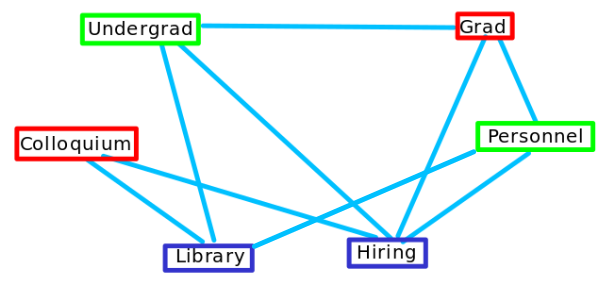
\includegraphics[scale=0.5]{../images/1.4.16.sol.png}
\end{figure}

So we can do the following:

Time 1: BLUE: hiring, library

Time 2: GREEN: personnel, undergraduate education

Time 3: RED: graduate education, colloquium

(We could have also colored Colloquium with GREEN instead. That's another
valid solution.)
\end{proof}

\subsubsection{Problem 17}
A department wants to schedule final exams so that no student has more than one
exam on any given day. The vertices of the graph below show the courses that are
being taken by more than one student, with an edge connecting two vertices if
there is a student in both courses. Find a way to color the vertices of the
graph with only four colors so that no two adjacent vertices have the same color
and explain how to use the result to schedule the final exams.

\begin{figure}[ht!]
\centering
\includegraphics[scale=0.5]{../images/1.4.17.png}
\end{figure}

\begin{proof}
One possible solution:
\begin{figure}[ht!]
\centering
\includegraphics[scale=0.5]{../images/1.4.17.sol.png}
\end{figure}

We can schedule the exams of the:

green courses (MCS101 and MCS102) on Monday,

blue course (MCS135) on Tuesday,

red courses (MCS130 and MCS110) on Wednesday,

orange courses (MCS100 and MCS120) on Thursday.

Since there is no edge connecting any two courses of the same color, there are
no students taking two courses of the same color.
\end{proof}

\section{Chapter 2}

\subsection {Exercise Set 2.1}
{\bf In each of $1-4$ represent the common form of each argument using letters to stand for component sentences, and fill in the blanks so that the argument in part (b) has the same logical form as the argument in part (a).}

\subsubsection{Exercise 1}
(a)
If all integers are rational, then the number 1 is rational.

All integers are rational.

Therefore, the number 1 is rational.

\begin{proof}
Common form: 1) If $p$ then $q$. 2) $p$. 3) Therefore, $q$.
\end{proof}

(b)
If all algebraic expressions can be written in prefix notation, then \fbl.

Therefore, $(a + 2b)(a^2 - b)$ can be written in prefix notation.

\begin{proof}
If all algebraic expressions can be written in prefix notation, then \\ \underline{$(a + 2b)(a^2 - b)$ can be written in prefix notation.} (If $p$, then $q$.)

All algebraic expressions can be written in prefix notation. ($p$.)

Therefore, $(a + 2b)(a^2 - b)$ can be written in prefix notation. (Therefore, $q$.)
\end{proof}

\subsubsection{Exercise 2}
(a)
If all computer programs contain errors, then this program contains an error.

This program does not contain an error.

Therefore, it is not the case that all computer programs contain errors.

\begin{proof}
Common form: 1) If $p$ then $q$. 2) $\sim q$. 3) Therefore, $\sim p$.
\end{proof}

(b)
If \fbl then \fbl.

$2$ is not odd.

Therefore, it is not the case that all prime numbers are odd.

\begin{proof}
If \underline{all prime numbers are odd} then \underline{2 is
odd}. (If $p$ then $q$.)

$2$ is not odd. ($\sim q$.)

Therefore, it is not the case that all prime numbers are odd. (Therefore, $\sim p$.)
\end{proof}

\subsubsection{Exercise 3}
(a)
This number is even or this number is odd.

This number is not even.

Therefore, this number is odd.

\begin{proof}
Common form: 1) $p \vee q$. 2) $\sim p$. 3) Therefore, $q$.
\end{proof}

(b)
\fbl or logic is confusing.

My mind is not shot.

Therefore, \fbl.

\begin{proof}
\underline{My mind is shot} or logic is confusing. ($p \vee q$.)

My mind is not shot. ($\sim p$.)

Therefore, \underline{logic is confusing}. (Therefore, $q$.) \end{proof}

\subsubsection{Exercise 4}
(a)
If the program syntax is faulty, then the computer will generate an error message.

If the computer generates an error message, then the program will not run.

Therefore, if the program syntax is faulty, then the program will not run.

\begin{proof}
Common form: 1) If $p$ then $q$. 2) If $q$ then $r$. 3) Therefore, if $p$ then $r$.
\end{proof}

(b)
If this simple graph \fbl, then it is complete.

If this graph \fbl, then any two of its vertices can be joined by a path.

Therefore, if this simple graph has 4 vertices and 6 edges, then \fbl.

\begin{proof}
If this simple graph \underline{has 4 vertices and 6 edges}, then it is complete.

If this graph \underline{is complete}, then any two of its vertices can be joined by a path.

Therefore, if this simple graph has 4 vertices and 6 edges, then \underline{any two of its vertices} \underline{can be joined by a path}.
\end{proof}

\subsubsection{Exercise 5}
Indicate which of the following sentences are statements.

(a)
1,024 is the smallest four-digit number that is a perfect square.

\begin{proof}
It is a statement because it is a true sentence. 1,024 is a perfect square because $1,024 = 32^2$, and the next smaller perfect square is $31^2 = 961$, which has fewer than four digits.
\end{proof}

(b)
She is a mathematics major.

\begin{proof}
It is not a statement because its truth value depends on the ``She''. (Here ``She'' can be thought of as a variable, like $x$.)
\end{proof}

(c)
$128 = 2^6$

\begin{proof}
It is a statement because it is false: $2^6 = 64 \neq 128$.
\end{proof}

(d)
$x = 2^6$

\begin{proof}
Not a statement, because its truth depends on the value of $x$.
\end{proof}

{\bf Write the statements in $6-9$ in symbolic form using the symbols $\sim$, $\vee$ and $\wedge$ and the indicated letters to represent component statements.}

\subsubsection{Exercise 6}
Let $s =$ “stocks are increasing” and $i =$ “interest rates are steady.”

(a)
Stocks are increasing but interest rates are steady.

\begin{proof}
$s \wedge i$.

(Notice that the ``but'' makes it sound like there should be a negation involved, but that's just a quirk of English. In this case, ``but'' has the same meaning as ``and''.

We have an intuitive expectation that there should be some ``causal link'' between stocks and interest rates, like: ``stocks are increasing, that should affect interest rates'', so if the interest rates are remaining steady, it's as if they are remaining steady DESPITE the fact that stocks are increasing, hence the ``but'' being used.)
\end{proof}

(b)
Neither are stocks increasing nor are interest rates steady.

\begin{proof}
${\sim s} \wedge {\sim i}$.

(Another quirk of English: when ``neither nor'' is used, even though ``nor'' sounds like there should be an OR involved, it's actually AND and negation.)
\end{proof}

\subsubsection{Exercise 7}
Juan is a math major but not a computer science major. ($m =$ “Juan is a math major,” $c =$ “Juan is a computer science major”)

\begin{proof}
$m \wedge {\sim c}$
\end{proof}

\subsubsection{Exercise 8}
Let $h =$ “John is healthy,” $w =$ “John is wealthy,” and $s =$ “John is wise.”

(a)
John is healthy and wealthy but not wise.

\begin{proof}
$h \wedge w \wedge {\sim s}$.
\end{proof}

(b)
John is not wealthy but he is healthy and wise.

\begin{proof}
${\sim w} \wedge h \wedge s$.
\end{proof}

(c)
John is neither healthy, wealthy, nor wise.

\begin{proof}
${\sim h} \wedge {\sim w} \wedge {\sim s}$.
\end{proof}

(d)
John is neither wealthy nor wise, but he is healthy.

\begin{proof}
$({\sim w} \wedge {\sim s}) \wedge h$.
\end{proof}

(e)
John is wealthy, but he is not both healthy and wise.

\begin{proof}
$w \wedge {\sim (h \wedge s)}$.
\end{proof}

\subsubsection{Exercise 9}
Let $p =$ “$x > 5$,” $q =$ “$x = 5$,” and $r =$ “$10 > x$.”

(a)
$x \geq 5$

\begin{proof}
$x \geq 5$ means $x > 5$ or $x = 5$. So: $p \vee q$.
\end{proof}

(b) $10 > x > 5$

\begin{proof}
$10 > x > 5$ means $10 > x$ and $x > 5$. So: $r \wedge p$.
\end{proof}

(c)
$10 > x \geq 5$

\begin{proof}
$10 > x \geq 5$ means $10 > x$ and $x \geq 5$, i.e. $10 > x$ and
($x > 5$ or $x = 5$).

So: $r \wedge (p \vee q)$.
\end{proof}

\subsubsection{Exercise 10}
Let $p$ be the statement “DATAENDFLAG is off,” $q$ the statement “ERROR equals 0,” and $r$ the statement “SUM is less than 1,000.” Express the following sentences in symbolic notation.

(a)
DATAENDFLAG is off, ERROR equals 0, and SUM is less than 1,000.

\begin{proof}
$p \wedge q \wedge r$.
\end{proof}

(b)
DATAENDFLAG is off but ERROR is not equal to 0.

\begin{proof}
$p \wedge {\sim q}$.
\end{proof}

(c)
DATAENDFLAG is off; however, ERROR is not 0 or SUM is greater than or equal to 1,000.

\begin{proof}
$p \wedge ({\sim q} \vee {\sim r})$.
\end{proof}

(d)
DATAENDFLAG is on and ERROR equals 0 but SUM is greater than
or equal to 1,000.

\begin{proof}
${\sim p} \wedge q \wedge {\sim r}$.
\end{proof}

(e)
Either DATAENDFLAG is on or it is the case that both ERROR equals 0 and SUM is less than 1,000.

\begin{proof}
${\sim p} \vee (q \wedge r)$.
\end{proof}

\subsubsection{Exercise 11}
In the following sentence, is the word ``or'' used in its inclusive or exclusive sense? A team wins the playoffs if it wins two games in a row or a total of three games.

\begin{proof}
Inclusive or. For instance, a team could win the playoff by winning games 1, 3, and 4 and losing game 2. Such an outcome would satisfy both conditions.
\end{proof}

{\bf Write truth tables for the statement forms in $12-15$.}

\subsubsection{Exercise 12}
${\sim p} \wedge q$

\begin{proof}
$$
\begin{array}{|cc|c|c|}
\hline p & q & {\sim p} & {\sim p} \wedge q \\
\hline T & T & F & F \\
\hline T & F & F & F \\
\hline F & T & T & T \\
\hline F & F & T & F \\
\hline \end{array}
$$
\end{proof}

\subsubsection{Exercise 13}
${\sim(p \wedge q)} \vee (p \vee q)$

\begin{proof}
This is a tautology:
$$
\begin{array}{|cc|c|c|c|c|c|}
\hline p & q & p \wedge q & {\sim (p \wedge q)} & p \vee q & {\sim(p \wedge q)} \vee (p \vee q) \\
\hline T & T & T & F & T & T \\
\hline T & F & F & T & T & T \\
\hline F & T & F & T & T & T \\
\hline F & F & F & T & F & T \\
\hline
\end{array}
$$
\end{proof}

\subsubsection{Exercise 14}
$p \wedge (q \wedge r)$

\begin{proof}
$$
\begin{array}{|ccc|c|}
\hline
p & q & r & p \wedge q \wedge r \\
\hline
T & T & T & T \\
\hline
T & T & F & F \\
\hline
T & F & T & F \\
\hline
T & F & F & F \\
\hline
F & T & T & F \\
\hline
F & T & F & F \\
\hline
F & F & T & F \\
\hline
F & F & F & F \\
\hline
\end{array}
$$
\end{proof}

\subsubsection{Exercise 15}
$p \wedge ({\sim q} \vee r)$

\begin{proof}
$$
\begin{array}{|ccc|c|c|}
\hline
p & q & r & {\sim q} \vee r & p \wedge ({\sim q} \vee r) \\ \hline
T & T & T & T & T \\
\hline
T & T & F & F & F \\
\hline
T & F & T & T & T \\
\hline
T & F & F & T & T \\
\hline
F & T & T & T & F \\
\hline
F & T & F & F & F \\
\hline
F & F & T & T & F \\
\hline
F & F & F & T & F \\
\hline
\end{array}
$$
\end{proof}

{\bf Determine whether the statement forms in $16-24$ are logically equivalent. In each case, construct a truth table and include a sentence justifying your answer. Your sentence should show that you understand the meaning of logical equivalence.}

\subsubsection{Exercise 16}
$p \vee (p \wedge q)$ and $p$

\begin{proof}
$$
\begin{array}{|cc|c|c|}
\hline
p & q & p \wedge q & p \vee (p \wedge q) \\
\hline
T & T & T & T \\
\hline
T & F & F & T \\
\hline
F & T & F & F \\
\hline
F & F & F & F \\
\hline
\end{array}
$$

$p \vee (p \wedge q)$ and $p$ always have the same truth values, so they are logically equivalent. (This proves one of the absorption laws.)
\end{proof}

\subsubsection{Exercise 17}
${\sim(p \wedge q)}$ and ${\sim p} \wedge {\sim q}$

\begin{proof}
$$
\begin{array}{|cc|c|c|}
\hline
p & q & {\sim(p \wedge q)} & {\sim p} \wedge {\sim q} \\
\hline
T & T & F & F \\
\hline
T & F & T & F \\
\hline
F & T & T & F \\
\hline
F & F & T & T \\
\hline
\end{array}
$$
Not logically equivalent. When $p = T$ and $q = F$ we have

${\sim (p \wedge q)} \equiv {\sim (T \wedge F)} \equiv {\sim F} \equiv T$, but

${\sim p} \wedge {\sim q} \equiv {\sim T \wedge {\sim F}} \equiv F \wedge T \equiv F$.
\end{proof}

\subsubsection{Exercise 18}
$p \vee \true$ and \true

\begin{proof}
$$
\begin{array}{|cc|c|}
\hline
p & \true & p \vee \true \\
\hline
T & T & T \\
\hline
F & T & T \\
\hline
\end{array}
$$

$\true$ and $p \vee \true$ always have the same truth values, so they are logically equivalent. (This proves one of the universal bound laws.)

\end{proof}

\subsubsection{Exercise 19}
$p \wedge \true$ and $p$

\begin{proof}
$$
\begin{array}{|cc|c|}
\hline
p & \true & p \wedge \true \\
\hline
T & T & T \\
\hline
F & T & F \\
\hline
\end{array}
$$

$p \wedge \true$ and $p$ always have the same truth values, so they are logically equivalent.
\end{proof}

\subsubsection{Exercise 20}
$p \wedge \false$ and $p \vee \false$

\begin{proof}
$$
\begin{array}{|cc|c|c|}
\hline
p & \false & p \wedge \false & p \vee \false \\
\hline
T & F & F & T \\
\hline
F & F & F & F \\
\hline
\end{array} $$

$p \wedge \false$ and $p \vee \false$ are not logically equivalent.
\end{proof}

\subsubsection{Exercise 21}
$(p \wedge q) \wedge r$ and $p \wedge (q \wedge r)$

\begin{proof}
$$
\begin{array}{|ccc|c|c|c|c|}
\hline
p & q & r & p \wedge q & q \wedge r & (p \wedge q) \wedge r & p \wedge (q \wedge r) \\
\hline
T & T & T & T & T & T & T \\
\hline
T & T & F & T & F & F & F \\
\hline
T & F & T & F & F & F & F \\
\hline
T & F & F & F & F & F & F \\
\hline
F & T & T & F & T & F & F \\
\hline
F & T & F & F & F & F & F \\
\hline
F & F & T & T & F & F & F \\
\hline
F & F & F & F & F & F & F \\
\hline
\end{array}
$$

$(p \wedge q) \wedge r$ and $p \wedge (q \wedge r)$ always have the same truth values, so they are logically equivalent. (This proves the associative law for $\wedge$.)
\end{proof}

\subsubsection{Exercise 22}
$p \wedge (q \vee r)$ and $(p \wedge q) \vee (p \wedge r)$

\begin{proof}
$$
\begin{array}{|ccc|c|c|c|c|c|}
\hline
p & q & r & p \wedge q & p \wedge r & q \vee r & p \wedge (q \vee r) & (p \wedge q) \vee (p \wedge r) \\
\hline
T & T & T & T & T & T & T & T \\
\hline
T & T & F & T & F & T & T & T \\
\hline
T & F & T & F & T & T & T & T \\
\hline
T & F & F & F & F & F & F & F \\
\hline
F & T & T & F & F & T & F & F \\
\hline
F & T & F & F & F & T & F & F \\
\hline
F & F & T & F & F & T & F & F \\
\hline
F & F & F & F & F & F & F & F \\
\hline
\end{array}
$$

$p \wedge (q \vee r)$ and $(p \wedge q) \vee (p \wedge r)$ always have the same truth values, so they are logically equivalent. (This proves one of the distributive laws for $\wedge$.)
\end{proof}

\subsubsection{Exercise 23}
$(p \wedge q) \vee r$ and $p \wedge (q \vee r)$

\begin{proof}
$$
\begin{array}{|ccc|c|c|c|c|}
\hline
p & q & r & p \wedge q & q \vee r & (p \wedge q) \vee r & p \wedge (q \vee r) \\
\hline
T & T & T & T & T & T & T \\
\hline
T & T & F & T & T & T & T \\
\hline
T & F & T & F & T & T & T \\
\hline
T & F & F & F & F & F & F \\
\hline
F & T & T & F & T & T & F \\
\hline
F & T & F & F & T & F & F \\
\hline
F & F & T & F & T & T & F \\
\hline
F & F & F & F & F & F & F \\
\hline
\end{array}
$$

$(p \wedge q) \vee r$ and $p \wedge (q \vee r)$ have different truth values in the fifth and seventh rows, so they are not logically equivalent. (This proves that parentheses are needed with $\wedge$ and $\vee$.)
\end{proof}

\subsubsection{Exercise 24}
$(p \vee q) \vee (p \wedge r)$ and $(p \vee q) \wedge r$

\begin{proof}
$$
\begin{array}{|ccc|c|c|c|c|}
\hline
p & q & r & p \vee q & p \wedge r & (p \vee q) \vee (p \wedge r) & (p \vee q) \wedge r \\
\hline
T & T & T & T & T & T & T \\
\hline
T & T & F & T & F & T & F \\
\hline
T & F & T & T & T & T & T \\
\hline
T & F & F & T & F & T & F \\
\hline
F & T & T & T & F & T & T \\
\hline
F & T & F & T & F & T & F \\
\hline
F & F & T & F & F & F & F \\
\hline
F & F & F & F & F & F & F \\
\hline
\end{array}
$$

$(p \vee q) \vee (p \wedge r)$ and $(p \vee q) \wedge r$ have different truth values in the fifth and seventh rows, so they are not logically equivalent.
\end{proof}

{\bf Use De Morgan’s laws to write negations for the statements in $25-30$.}

\subsubsection{Exercise 25}
Hal is a math major and Hal’s sister is a computer science major.

\begin{proof}
$p =$ Hal is a math major, $q =$ Hal’s sister is a computer science major

The statement is $p \wedge q$. By De Morgan's laws, the negation is $\sim(p \wedge q) \equiv {\sim p} \vee {\sim q}$:

Hal is not a math major, or Hal's sister is not a computer science major.
\end{proof}

\subsubsection{Exercise 26}
Sam is an orange belt and Kate is a red belt.

\begin{proof}
$p =$ Sam is an orange belt, $q =$ Kate is a red belt.

The statement is $p \wedge q$. By De Morgan's laws, the negation is $\sim(p \wedge q) \equiv {\sim p} \vee {\sim q}$:

Sam is not an orange belt, or Kate is not a red belt. \end{proof}

\subsubsection{Exercise 27}
The connector is loose or the machine is unplugged.

\begin{proof}
$p =$ The connector is loose, $q =$ the machine is unplugged.

The statement is $p \vee q$. By De Morgan's laws, the negation is $\sim(p \vee q) \equiv {\sim p} \wedge {\sim q}$:

The connector is not loose and the machine is not unplugged. \end{proof}

\subsubsection{Exercise 28}
The train is late or my watch is fast.

\begin{proof}
$p =$ The train is late, $q =$ my watch is fast.

The statement is $p \vee q$. By De Morgan's laws, the negation is $\sim(p \vee q) \equiv {\sim p} \wedge {\sim q}$:

The train is not late and my watch is not fast.
\end{proof}

\subsubsection{Exercise 29}
This computer program has a logical error in the first ten lines or it is being run with an incomplete data set.

\begin{proof}
$p =$ This computer program has a logical error in the first ten lines, $q =$ it (this computer) is being run with an incomplete data set.

The statement is $p \vee q$. By De Morgan's laws, the negation is $\sim(p \vee q) \equiv {\sim p} \wedge {\sim q}$:

This computer program does not have a logical error in the first ten lines and it is not being run with an incomplete data set.
\end{proof}

\subsubsection{Exercise 30}
The dollar is at an all-time high and the stock market is at a record low.

\begin{proof}
$p =$ The dollar is at an all-time high, $q =$ the stock market is at a record low.

The statement is $p \wedge q$. By De Morgan's laws, the negation is $\sim(p \wedge q) \equiv {\sim p} \vee {\sim q}$:

The dollar is not at an all-time high or the stock market is not at a record low.
\end{proof}

\subsubsection{Exercise 31}
Let $s$ be a string of length $2$ with characters from $\{0, 1, 2\}$, and define statements $a, b, c$, and $d$ as follows:

\begin{itemize}
\item $a = $ ``the first character of $s$ is $0$''
\item $b = $ ``the first character of $s$ is $1$''
\item $c = $ ``the second character of $s$ is $1$''
\item $d = $ ``the second character of $s$ is $2$'' \end{itemize}

Describe the set of all strings for which each of the following is true.

(Here are all the possible length 2 strings: 00, 01, 02, 10, 11, 12, 20, 21, 22)

(a)
$(a \vee b) \wedge (c \vee d)$

\begin{proof}
This translates to: ``the first character is 0 or 1, and the second character is1 or 2''. So the answer is: 01, 02, 11, 12
\end{proof}

(b)
$({\sim(a \vee b)}) \wedge (c \vee d)$

\begin{proof}
This translates to: ``the first character is not 0 or 1, and the second character is 1 or 2''. So the answer is: 21, 22
\end{proof}

(c)
$(({\sim a}) \vee b) \wedge (c \vee ({\sim d}))$

\begin{proof}
This translates to: ``the first character is not 0 or it is 1, and the second character is 1 or is not 2''.

So the first character can be 1 or 2, and the second character can be 0 or 1.

So the answer is: 10, 11, 20, 21
\end{proof}

{\bf Assume $x$ is a particular real number and use De Morgan’s laws to write negations for the statements in $32-37$.}

\subsubsection{Exercise 32}
$-2 < x < 7$

\begin{proof}
This is $(-2 < x) \wedge (x < 7)$. Keep in mind that the negation of $<$ is $\geq$. By De Morgan, the negation is

$\sim((-2 < x) \wedge (x < 7)) \equiv {\sim(-2 < x)} \vee {\sim(x < 7)} \equiv (-2 \geq x) \vee (x \geq 7)$

The answer is: $-2 \geq x$ or $x \geq 7$.
\end{proof}

\subsubsection{Exercise 33}
$-10 < x < 2$

\begin{proof}
Similar to 32, the answer is: $-10 \geq x$ or $x \geq 2$.
\end{proof}

\subsubsection{Exercise 34}
$x < 2$ or $x > 5$

\begin{proof}
The negation of $>$ is $\leq$. By De Morgan, the negation is:

${\sim(x < 2 \vee x > 5)} \equiv {\sim (x < 2)} \wedge {\sim (x > 5)} \equiv (x \geq 2) \wedge (x \leq 5)$

The answer is: $2 \leq x \leq 5$.
\end{proof}

\subsubsection{Exercise 35}
$x \leq -1$ or $x > 1$

\begin{proof}
Similar to 34. The answer is: $-1 < x \leq 1$.
\end{proof}

\subsubsection{Exercise 36}
$1 > x \geq -3$

\begin{proof}
Rewriting this as $-3 \leq x < 1$, we see that it is similar to 32 and 33.

The answer is: $-3 > x$ or $x \geq 1$. In other words: $1 \leq x$ or $x < -3$.
\end{proof}

\subsubsection{Exercise 37}
$0 > x \geq -7$

\begin{proof}
This is just like 36. The answer is: $0 \leq x$ or $x < -7$.
\end{proof}

{\bf In 38 and 39, imagine that {\it num\_orders} and {\it num\_instock} are particular values, such as might occur during execution of a computer program. Write negations for the following statements.}

\subsubsection{Exercise 38}
$(num\_orders > 100$ and $num\_instock \leq 500)$ or
$num\_instock < 200$

\begin{proof}
This statement’s logical form is $(p \wedge q) \vee r$, so its negation has the form

$$
{\sim((p \wedge q) \vee r)} \equiv {\sim (p \wedge q)} \wedge {\sim r} \equiv ({\sim p} \vee {\sim q}) \wedge {\sim r}
$$

Thus a negation for the statement is:

$(num\_orders \leq 100$ or $num\_instock > 500)$ and $num\_instock \geq 200$.
\end{proof}

\subsubsection{Exercise 39}
$(num\_orders < 50$ and $num\_instock > 300)$ \\
or $(50 \leq num\_orders < 75$ and $num\_instock > 500)$

\begin{proof}
This statement’s logical form is $(p \wedge q) \vee ({\sim p}
\wedge r \wedge s)$, so its negation has the form

$$
{\sim((p \wedge q) \vee ({\sim p} \wedge r \wedge s))} \equiv {\sim(p \wedge q)} \wedge {\sim({\sim p} \wedge r \wedge s)} \equiv ({\sim p} \vee {\sim q}) \wedge (p \vee {\sim r} \vee {\sim s})
$$

Thus a negation for the statement is:

$(num\_orders \geq 50$ or $num\_instock \leq 300)$ and

($num\_orders < 50$ or $num\_orders \geq 75$ or $num\_instock \leq 500$).
\end{proof}

{\bf Use truth tables to establish which of the statement forms in $40-43$ are tautologies and which are contradictions.}

\subsubsection{Exercise 40}
$(p \wedge q) \vee ({\sim p} \vee (p \wedge {\sim q}))$

\begin{proof}
$$
\begin{array}{|cc|c|c|c|c|c|c|}
\hline
p & q & {\sim p} & {\sim q} & p \wedge q & p \wedge {\sim q} & {\sim p} \vee (p \wedge {\sim q}) & (p \wedge q) \vee ({\sim p} \vee (p \wedge {\sim q})) \\
\hline
T & T & F & F & T & F & F & T \\
\hline
T & F & F & T & F & T & T & T \\
\hline
F & T & T & F & F & F & T & T \\
\hline
F & F & T & T & F & F & T & T \\
\hline
\end{array}
$$
We see that $(p \wedge q) \vee ({\sim p} \vee (p \wedge {\sim q}))$ is a tautology.
\end{proof}

\subsubsection{Exercise 41}
$(p \wedge {\sim q}) \wedge ({\sim p} \vee q))$

\begin{proof}
$$
\begin{array}{|cc|c|c|c|c|c|}
\hline
p & q & {\sim p} & {\sim q} & p \wedge {\sim q} & {\sim p} \vee q & (p \wedge {\sim q}) \wedge ({\sim p} \vee q) \\
\hline
T & T & F & F & F & T & F \\
\hline
T & F & F & T & T & F & F \\
\hline
F & T & T & F & F & T & F \\
\hline
F & F & T & T & F & T & F \\
\hline
\end{array}
$$
$(p \wedge {\sim q}) \wedge ({\sim p} \vee q)$ is always false, so it is a contradiction.
\end{proof}

\subsubsection{Exercise 42} $(({\sim p} \wedge q) \wedge (q \wedge r))) \wedge
{\sim q}$

\begin{proof}
$$
\begin{array}{|ccc|c|c|c|c|}
\hline
p & q & r & {\sim p} \vee q & q \wedge r & ({\sim p} \vee q) \wedge (q \wedge r)& (({\sim p} \wedge q) \wedge (q \wedge r))) \wedge {\sim q} \\
\hline
T & T & T & T & T & T & F \\
\hline
T & T & F & T & F & F & F \\
\hline
T & F & T & F & F & F & F \\
\hline
T & F & F & F & F & F & F \\
\hline
F & T & T & T & T & T & F \\
\hline
F & T & F & T & F & F & F \\
\hline
F & F & T & T & F & F & F \\
\hline
F & F & F & T & F & F & F \\
\hline
\end{array}
$$
$(({\sim p} \wedge q) \wedge (q \wedge r))) \wedge {\sim q}$ is a contradiction.
\end{proof}

\subsubsection{Exercise 43}
$({\sim p} \vee q) \vee (p \wedge {\sim q})$

\begin{proof}
$$
\begin{array}{|cc|c|c|c|c|c|}
\hline
p & q & {\sim p} & {\sim q} & {\sim p} \vee q & p \wedge {\sim q} & ({\sim p} \vee q) \vee (p \wedge {\sim q}) \\
\hline
T & T & F & F & T & F & T \\
\hline
T & F & F & T & F & T & T \\
\hline
F & T & T & F & T & F & T \\
\hline
F & F & T & T & T & F & T \\
\hline
\end{array}
$$
We see that $({\sim p} \vee q) \vee (p \wedge {\sim q})$ is a tautology.
\end{proof}

\subsubsection{Exercise 44}
Recall that $a < x < b$ means that $a < x$ and $x < b$. Also $a \leq b$ means that $a < b$ or $a = b$. Find all real numbers $x$ that satisfy the following inequalities.

(a)
$2 < x \leq 0$

\begin{proof}
No real numbers satisfy this inequality. If $x > 2$ then $x > 2 > 0$ so $x > 0$.Therefore $x \leq 0$ cannot be true at the same time.
\end{proof}

(b)
$1 \leq x < -1$

\begin{proof}
Similar to (a). no real numbers satisfy this inequality.
\end{proof}

\subsubsection{Exercise 45}
Determine whether the statements in (a) and (b) are logically equivalent.

(a) Bob is both a math and computer science major and Ann is a math major, but Ann is not both a math and computer science major.

(b) It is not the case that both Bob and Ann are both math and computer science majors, but it is the case that Ann is a math major and Bob is both a math and computer science major.

\begin{proof} Define
\begin{enumerate}
\item $p$: Bob is a math major.
\item $q$: Bob is a CS major.
\item $r$: Ann is a math major.
\item $s$: Ann is a CS major.
\end{enumerate}

The statement in (a) has the form: $(p \wedge q \wedge r) \wedge {\sim (r \wedge s)}$

The statement in (b) has the form: ${\sim (p \wedge q \wedge r \wedge s)} \wedge (r \wedge p \wedge q)$

We could write down the entire truth table with $2^4 = 16$ rows, but let's try to take some shortcuts.

If we look at the two expressions, they both have the form $(p \wedge q \wedge r) \wedge Z$. Such an expression is true when $(p \wedge q \wedge r)$ and $Z$ are both true, and it is false otherwise.

Therefore, when evaluating $Z$, we can concentrate only on the rows of the truth table where $(p \wedge q \wedge r)$ is true. We can disregard $Z$ on the other rows (because both (a) and (b) are false for those rows).

$(p \wedge q \wedge r)$ is true only when all 3 of $p, q, r$ are true. When this is the case, we only need to consider the possibilities for $s$. This gives us 2 rows only:
$$
\begin{array}{|c|c|c|}
\hline
s & {\sim (r \wedge s)} & {\sim (p \wedge q \wedge r \wedge s)} \\
\hline
T & F & F \\
\hline
F & T & T \\
\hline
\end{array}
$$

The two $Z$ expressions have the same truth values in all cases. Therefore (a) and (b) are logically equivalent.
\end{proof}

\subsubsection{Exercise 46}
Let the symbol $\oplus$ denote {\it exclusive or}; so $p \oplus q \equiv (p \vee q) \wedge {\sim(p \wedge q)}$. Hence the truth table for $p \oplus q$ is as follows:

\begin{center}
\begin{tabular}{|cc|c|}
\hline
$p$ & $q$ & $p \oplus q$ \\
\hline
T & T & F \\
\hline
T & F & T \\
\hline
F & T & T \\
\hline
F & F & F \\
\hline
\end{tabular}
\end{center}

(a)
Find simpler statement forms that are logically equivalent to $p \oplus p$ and $(p \oplus p) \oplus p$.

\begin{proof}
The meaning of the exclusive or $\oplus$ is that, it returns true when the two operands have different truth values; otherwise it returns false.

In $p \oplus p$, the two operands $p$ and $p$ always have the same truth value. Therefore $p \oplus p$ is a contradiction: $p \oplus p \equiv \false$.

So we have $(p \oplus p) \oplus p \equiv \false \oplus p$. This is true only when $p$ and $\false$ have different truth values, in other words, when $p$ is true. Therefore $\false \oplus p$ is logically equivalent to $p$.
\end{proof}

(b)
Is $(p \oplus q) \oplus r \equiv p \oplus (q \oplus r)$? Justify your answer.

\begin{proof}
$$
\begin{array}{|ccc|c|c|c|c|}
\hline
p & q & r & p \oplus q & q \oplus r & (p \oplus q) \oplus r & p \oplus (q \oplus r) \\
\hline
T & T & T & F & F & T & T \\
\hline
T & T & F & F & T & F & F \\
\hline
T & F & T & T & T & F & F \\
\hline
T & F & F & T & F & T & T \\
\hline
F & T & T & T & F & F & F \\
\hline
F & T & F & T & T & T & T \\
\hline
F & F & T & F & T & T & T \\
\hline
F & F & F & F & F & F & F \\
\hline
\end{array}
$$
They are logically equivalent.
\end{proof}

(c)
Is $(p \oplus q) \wedge r \equiv (p \wedge r) \oplus (q \wedge r)$? Justify your answer.

\begin{proof}
$$
\begin{array}{|ccc|c|c|c|c|c|}
\hline
p & q & r & p \oplus q & p \wedge r & q \wedge r & (p \oplus q) \wedge r & (p \wedge r) \oplus (q \wedge r) \\
\hline
T & T & T & F & T & T & F & F \\
\hline
T & T & F & F & F & F & F & F \\
\hline
T & F & T & T & T & F & T & T \\
\hline
T & F & F & T & F & F & F & F \\
\hline
F & T & T & T & F & T & T & T \\
\hline
F & T & F & T & F & F & F & F \\
\hline
F & F & T & F & F & F & F & F \\
\hline
F & F & F & F & F & F & F & F \\
\hline
\end{array}
$$
They are logically equivalent.
\end{proof}

\subsubsection{Exercise 47}
In logic and in standard English, a double negative is equivalent to a positive.There is one fairly common English usage in which a “double positive” is equivalent to a negative. What is it? Can you think of others?

\begin{proof} There is a famous story about a philosopher who once gave a talk in which he observed that whereas in English and many other languages a double negative is equivalent to a positive, there is no language in which a double positive is equivalent to a negative. To this, another philosopher, Sidney
Morgenbesser, responded sarcastically, “Yeah, yeah.”

{\it [Strictly speaking, sarcasm functions like negation. When spoken sarcastically, the words “Yeah, yeah” are not a true double positive; they just mean “no.”]}
\end{proof}

{\bf In 48 and 49 below, a logical equivalence is derived from Theorem 2.1.1. Supply a reason for each step.}

\subsubsection{Exercise 48}
$$
\begin{array}{rcll}
(p \wedge {\sim q}) \vee (p \wedge q) & \equiv & p \wedge ({\sim q} \vee q) & \text{by (a)} \\
& \equiv & p \wedge (q \vee {\sim q}) & \text{by (b)} \\
& \equiv & p \wedge \true & \text{by (c)} \\
& \equiv & p & \text{by (d)} \\
\end{array}
$$
Therefore, $(p \wedge {\sim q}) \vee (p \wedge q) \equiv p$.

\begin{proof}
(a) is the distributive law. (b) is the commutative law for
$\vee$. (c) is the negation law for $\vee$. (d) is the identity law for $\wedge$.
\end{proof}

\subsubsection{Exercise 49}
$$
\begin{array}{rcll}
(p \vee {\sim q}) \wedge ({\sim p} \vee {\sim q}) & \equiv & ({\sim q} \vee p) \wedge ({\sim q} \vee {\sim p}) & \text{by (a)} \\
& \equiv & {\sim q} \vee (p \wedge {\sim p}) & \text{by (b)} \\
& \equiv & {\sim q} \vee \false & \text{by (c)} \\
& \equiv & {\sim q} & \text{by (d)} \\
\end{array}
$$

Therefore, $(p \vee {\sim q}) \wedge ({\sim p} \vee {\sim q}) \equiv {\sim q}$.

\begin{proof}
(a) is the commutative law for $\vee$. (b) is the distributive
law. (c) is the negation law for $\wedge$. (d) is the identity law for $\vee$.
\end{proof}

{\bf Use Theorem 2.1.1 to verify the logical equivalences in $50-54$. Supply a reason for each step.}

\subsubsection{Exercise 50}
$(p \wedge {\sim q}) \vee p \equiv p$

\begin{proof}
$(p \wedge {\sim q}) \vee p$
\begin{tabular}{rclr}
& $\equiv$ & $p \vee (p \wedge {\sim q})$ & (by the commutative law for $\vee$) \\
& $\equiv$ & $p$ & (by the absorption law for $\vee$) \\
\end{tabular}
\end{proof}

\subsubsection{Exercise 51}
$p \wedge ({\sim q} \vee p) \equiv p$

\begin{proof}
$p \wedge ({\sim q} \vee p)$
\begin{tabular}{rclr}
& $\equiv$ & $p \wedge (p \vee {\sim q})$ & (by the commutative law for $\vee$) \\
& $\equiv$ & $p$ & (by the absorption law for $\wedge$) \\
\end{tabular}
\end{proof}

\subsubsection{Exercise 52}
${\sim (p \vee {\sim q})} \vee ({\sim p} \wedge {\sim q}) \equiv {\sim p}$

\begin{proof}
${\sim (p \vee {\sim q})} \vee ({\sim p} \wedge {\sim q})$

\begin{tabular}{rcll}
& $\equiv$ & $({\sim p} \wedge q) \vee ({\sim p} \wedge {\sim q})$ & (by De Morgan laws) \\
& $\equiv$ & ${\sim p} \wedge (q \vee {\sim q})$ & (by distributive law for $\wedge$) \\
& $\equiv$ & ${\sim p} \wedge \true$ & (by negation law for $\vee$) \\
& $\equiv$ & ${\sim p}$ & (by identity law for $\wedge$) \\ \end{tabular}
\end{proof}

\subsubsection{Exercise 53} $\sim(({\sim p} \wedge q) \vee ({\sim p} \wedge {\sim
q})) \vee (p \wedge q) \equiv p$

\begin{proof} $\sim(({\sim p} \wedge q) \vee ({\sim p} \wedge {\sim q})) \vee (p
\wedge q)$

\begin{tabular}{rcll}
& $\equiv$ & $\sim({\sim p} \wedge (q \vee {\sim q})) \vee
(p \wedge q)$ & (by the distributive law) \\
& $\equiv$ & $\sim({\sim p} \wedge
\true) \vee (p \wedge q)$ & (by the negation law for $\vee$) \\
& $\equiv$ & $\sim({\sim p}) \vee (p \wedge q)$ & (by the identity law for $\vee$) \\
& $\equiv$ & $p \vee (p \wedge q)$ & (by the double negative law) \\
& $\equiv$ & $p$ & (by the absorption law) \\
\end{tabular}
\end{proof}

\subsubsection{Exercise 54}
$(p \wedge ({\sim ({\sim p} \vee q)})) \vee (p \wedge q) \equiv p$

\begin{proof}
$(p \wedge ({\sim ({\sim p} \vee q)})) \vee (p \wedge q)$

\begin{tabular}{rcll}
& $\equiv$ & $(p \wedge (p \wedge {\sim q})) \vee (p \wedge q)$ & (by De Morgan law) \\
& $\equiv$ & $((p \wedge p) \wedge {\sim q}) \vee (p \wedge q)$ & (by the associative law) \\
& $\equiv$ & $(p \wedge {\sim q}) \vee (p \wedge q)$ & (by the idempotent law) \\
 & $\equiv$ & $p \wedge ({\sim q} \vee q)$ & (by the distributive law) \\
& $\equiv$ & $p \wedge \true$ & (by the negation law) \\
& $\equiv$ & $p$ & (by the identity law) \\
\end{tabular}
\end{proof}

\subsection{Exercise Set 2.2}
{\bf Rewrite the statements in $1-4$ in if-then form.}

\subsubsection{Exercise 1}
This loop will repeat exactly $N$ times if it does not contain a stop or a go to.

\begin{proof}
If this loop does not contain a stop or a go to, then it will
repeat exactly $N$ times.
\end{proof}

\subsubsection{Exercise 2}
I am on time for work if I catch the 8:05 bus.

\begin{proof}
If I catch the 8:05 bus then I am on time for work.
\end{proof}

\subsubsection{Exercise 3} Freeze or I’ll shoot.

\begin{proof}
If you do not freeze, then I’ll shoot.
\end{proof}

\subsubsection{Exercise 4}
Fix my ceiling or I won’t pay my rent.

\begin{proof}
If you do not fix my ceiling then I won't pay my rent.
\end{proof}

{\bf Construct truth tables for the statement forms in $5-11$.}

\subsubsection{Exercise 5}
${\sim p} \vee q \to {\sim q}$

\begin{proof}
$$
\begin{array}{|cc|c|c|c|c|}
\hline
p & q & {\sim p} & {\sim q} & {\sim p} \vee q & {\sim p} \vee q \to {\sim q} \\
\hline
T & T & F & F & T & F \\
\hline
T & F & F & T & F & T \\
\hline
F & T & T & F & T & F \\
\hline
F & F & T & T & T & T \\
\hline
\end{array}
$$
\end{proof}

\subsubsection{Exercise 6}
$(p \vee q) \vee ({\sim p} \wedge q) \to q$

\begin{proof}
$$
\begin{array}{|cc|c|c|c|c|c|}
\hline
p & q & {\sim p} & p \vee q & {\sim p} \wedge q & (p \vee q) \vee ({\sim p} \wedge q) & (p \vee q) \vee ({\sim p} \wedge q) \to q \\
\hline
T & T & F & T & F & T & T \\
\hline
T & F & F & T & F & T & F \\
\hline
F & T & T & T & T & T & T \\
\hline
F & F & T & F & F & F & T \\
\hline
\end{array}
$$
\end{proof}

\subsubsection{Exercise 7}
$p \wedge {\sim q} \to r$

\begin{proof}
$$
\begin{array}{|ccc|c|c|c|}
\hline
p & q & r & {\sim q} & p \wedge {\sim q} & p \wedge {\sim q} \to r \\
\hline
T & T & T & F & F & T \\
\hline
T & T & F & F & F & T \\
\hline
T & F & T & T & T & T \\
\hline
T & F & F & T & T & F \\
\hline
F & T & T & F & F & T \\
\hline
F & T & F & F & F & T \\
\hline
F & F & T & T & F & T \\
\hline
F & F & F & T & F & T \\
\hline
\end{array}
$$
\end{proof}

\subsubsection{Exercise 8}
${\sim p} \vee q \to r$

\begin{proof}
$$
\begin{array}{|ccc|c|c|c|}
\hline
p & q & r & {\sim p} & {\sim p} \vee q & {\sim p} \vee q \to r\\
\hline
T & T & T & F & T & T \\
\hline
T & T & F & F & T & F \\
\hline
T & F & T & F & F & T \\
\hline
T & F & F & F & F & T \\
\hline
F & T & T & T & T & T \\
\hline
F & T & F & T & T & F \\
\hline
F & F & T & T & T & T \\
\hline
F & F & F & T & T & F \\
\hline
\end{array}
$$
\end{proof}

\subsubsection{Exercise 9}
$p \wedge {\sim r} \bic q \vee r$

\begin{proof}
$$
\begin{array}{|ccc|c|c|c|c|}
\hline
p & q & r & {\sim r} & p \wedge {\sim r} & q \vee r & p \wedge {\sim r} \bic q \vee r \\
\hline
T & T & T & F & F & T & F \\
\hline
T & T & F & T & T & T & T \\
\hline
T & F & T & F & F & T & F \\
\hline
T & F & F & T & T & F & F \\
\hline
F & T & T & F & F & T & F \\
\hline
F & T & F & T & F & T & F \\
\hline
F & F & T & F & F & T & F \\
\hline
F & F & F & T & F & F & T \\
\hline
\end{array}
$$
\end{proof}

\subsubsection{Exercise 10}
$(p \to r) \bic (q \to r)$

\begin{proof}
$$
\begin{array}{|ccc|c|c|c|}
\hline
p & q & r & p \to r & q \to r & (p \to r) \bic (q \to r) \\
\hline
T & T & T & T & T & T \\
\hline
T & T & F & F & F & T \\
\hline
T & F & T & T & T & T \\
\hline
T & F & F & F & T & F \\
\hline
F & T & T & T & T & T \\
\hline
F & T & F & T & F & F \\
\hline
F & F & T & T & T & T \\
\hline
F & F & F & T & T & T \\
\hline
\end{array}
$$
\end{proof}

\subsubsection{Exercise 11}
$(p \to (q \to r)) \bic ((p \wedge q) \to r)$

\begin{proof}
$$
\begin{array}{|ccc|c|c|c|c|c|}
\hline
p & q & r & q \to r & p \to (q \to r) & (p \wedge q) & (p \wedge q) \to r & (p \to (q \to r)) \bic ((p \wedge q) \to r) \\
\hline
T & T & T & T & T & T & T & T\\
\hline
T & T & F & F & F & T & F & T\\
\hline
T & F & T & T & T & F & T & T\\
\hline
T & F & F & T & T & F & T & T\\
\hline
F & T & T & T & T & F & T & T\\
\hline
F & T & F & F & T & F & T & T\\
\hline
F & F & T & T & T & F & T & T\\
\hline
F & F & F & T & T & F & T & T\\
\hline
\end{array}
$$
\end{proof}

\subsubsection{Exercise 12}
Use the logical equivalence established in Example 2.2.3, $p \vee q \to r \equiv (p \to r) \wedge (q \to r)$, to rewrite the
following statement. (Assume that $x$ represents a fixed real number.)
\begin{center}
If $x > 2$ or $x < -2$ then $x^2 > 4$.
\end{center}

\begin{proof}
If $x > 2$ then $x^2 > 4$, and if $x < -2$ then $x^2 > 4$.
\end{proof}

\subsubsection{Exercise 13}
Use truth tables to verify the following logical equivalences. Include a few words of explanation with your answers.

(a)
$p \to q \equiv {\sim p} \vee q$

\begin{proof}
$$
\begin{array}{|cc|c|c|c|}
\hline
p & q & {\sim p} & p \to q & {\sim p} \vee q \\
\hline
T & T & F & T & T \\
\hline
T & F & F & F & F \\
\hline
F & T & T & T & T \\
\hline
F & F & T & T & T \\
\hline
\end{array}
$$
$p \to q$ and ${\sim p} \vee q$ always have the same truth values, therefore they are logically equivalent.
\end{proof}

(b)
${\sim (p \to q)} \equiv p \wedge {\sim q}$

\begin{proof}
$$
\begin{array}{|cc|c|c|c|}
\hline
p & q & {\sim q} & {\sim (p \to q)} & p \wedge {\sim q} \\ \hline
T & T & F & F & F \\
\hline
T & F & T & T & T \\
\hline
F & T & F & F & F \\
\hline
F & F & T & F & F \\
\hline
\end{array}
$$
${\sim (p \to q)}$ and $p \wedge {\sim q}$ always have the same truth values, therefore they are logically equivalent. \end{proof}

\subsubsection{Exercise 14}
(a)
Show that the following statement forms are all logically equivalent:

$p \to q \vee r$, \,\,\, $p \wedge {\sim q} \to r$, and $p \wedge {\sim r} \to q$

\begin{proof}
Repeatedly using the fact that $A \to B \equiv {\sim A} \vee B$, De Morgan laws and the double negation law:

$p \to q \vee r \equiv {\sim p} \vee (q \vee r)$.

$p \wedge {\sim q} \to r \equiv {\sim (p \wedge {\sim q}) \vee r} \equiv ({\sim p} \vee {\sim {\sim q}}) \vee r \equiv ({\sim p} \vee q) \vee r$.

$p \wedge {\sim r} \to q \equiv {\sim (p \wedge {\sim r}) \vee q} \equiv ({\sim p} \vee {\sim {\sim r}}) \vee q \equiv ({\sim p} \vee r) \vee q$.

These three are equivalent by the commutative and associative laws for $\vee$.
\end{proof}

(b)
Use the logical equivalences established in part (a) to rewrite the following sentence in two different ways. (Assume that $n$
represents a fixed integer.)

\begin{center}
If $n$ is prime, then $n$ is odd or $n$ is 2.
\end{center}

\begin{proof}
Here $p$: ``$n$ is prime'', $q$: ``$n$ is odd'', $r$: ``$n$ is
2''.

So the statement is $p \to q \vee r$.

By part (a) this is equivalent to both $p \wedge {\sim q} \to r$ and to $p \wedge {\sim r} \to q$:

If $n$ is prime and $n$ is not odd, then $n$ is 2.

If $n$ is prime and $n$ is not 2, then $n$ is odd.
\end{proof}

\subsubsection{Exercise 15}
Determine whether the following statement forms are logically equivalent:

$p \to (q \to r)$ and $(p \to q) \to r$

\begin{proof}
No. When all three are false, we have $p \to (q \to r) \equiv F \to (F \to F) \equiv F \to T \equiv T$;

however, we have $(p \to q) \to r \equiv (F \to F) \to F \equiv T \to F \equiv F$.
\end{proof}

{\bf In 16 and 17, write each of the two statements in symbolic form and determine whether they are logically equivalent. Include a truth table and a few words of explanation to show that you understand what it means for statements to be logically equivalent.}

\subsubsection{Exercise 16}
If you paid full price, you didn’t buy it at Crown Books. You didn’t buy it at Crown Books or you paid full price.

\begin{proof}
Let $p$ represent “You paid full price” and $q$ represent “You
didn’t buy it at Crown Books.” Thus, “If you paid full price, you didn’t buy it at Crown Books” has the form $p \to q$. And “You didn’t buy it at Crown Books or you paid full price” has the form $q \vee p$.
$$
\begin{array}{|cc|c|c|}
\hline
p & q & p \to q & q \vee p \\
\hline
T & T & T & T \\
\hline
T & F & F & T \\
\hline
F & T & T & T \\
\hline
F & F & T & F \\
\hline
\end{array}
$$
These two statements are not logically equivalent because their forms have different truth values in rows 2 and 4.

(An alternative representation for the forms of the two statements is $p \to {\sim q}$ and ${\sim q} \vee p$. In this case, the truth values differ in rows 1 and 3.)
\end{proof}

\subsubsection{Exercise 17}
If 2 is a factor of $n$ and 3 is a factor of $n$, then 6 is a factor of $n$. 2 is not a factor of $n$ or 3 is not a factor of $n$ or 6 is a factor of $n$.

\begin{proof}
Let $p$ represent “2 is a factor of $n$” and $q$ represent “3 is a factor of $n$” and $r$ represent ``6 is a factor of $n$''.

So the two statements have the forms: $p \wedge q \to r$ and ${\sim p} \vee {\sim q} \vee r$.
$$
\begin{array}{|ccc|c|c|c|}
\hline
p & q & r & p \wedge q & p \wedge q \to r & {\sim p} \vee {\sim q} \vee r \\
\hline
T & T & T & T & T & T \\
\hline
T & T & F & T & F & F \\
\hline
T & F & T & F & T & T \\
\hline
T & F & F & F & T & T \\
\hline
F & T & T & F & T & T \\
\hline
F & T & F & F & T & T \\
\hline
F & F & T & F & T & T \\
\hline
F & F & F & F & T & T \\
\hline
\end{array}
$$
These two statements are logically equivalent. We can also see this without the truth table: $p \wedge q \to r \equiv {\sim (p \wedge q)} \vee r \equiv ({\sim p} \vee {\sim q}) \vee r$. Here we used $A \to B \equiv {\sim A} \vee B$ and De Morgan laws. \end{proof}

\subsubsection{Exercise 18}
Write each of the following three statements in symbolic form and determine which pairs are logically equivalent. Include truth tables and a few words of explanation.

If it walks like a duck and it talks like a duck, then it is a duck.

Either it does not walk like a duck or it does not talk like a duck, or it is a duck.

If it does not walk like a duck and it does not talk like a duck, then it is not a duck.

\begin{proof}
They are: $p \wedge q \to r$ and ${\sim p} \vee {\sim q} \vee r$ and ${\sim p} \wedge {\sim q} \to {\sim r}$.

The first two are equivalent by Exercise 17. The last is not equivalent to the first two: when $p$ is true, $q$ is true and $r$ is false, we have

$p \wedge q \to r \equiv T \wedge T \to F \equiv T \to F \equiv F$, but

${\sim p} \wedge {\sim q} \to {\sim r} \equiv F \wedge F \to T \equiv F \to T \equiv T$.
\end{proof}

\subsubsection{Exercise 19} True or false? The negation of “If Sue is Luiz’s mother, then Ali is his cousin” is “If Sue is Luiz’s mother, then Ali is not his cousin.”

\begin{proof}
False. The negation of an if-then statement is not an if-then
statement. It is an and statement.
\end{proof}

\subsubsection{Exercise 20}
Write negations for each of the following statements. (Assume that all variables represent fixed quantities or entities, as
appropriate.)

(a)
If $P$ is a square, then $P$ is a rectangle.

\begin{proof}
$P$ is a square and $P$ is not a rectangle.
\end{proof}

(b)
If today is New Year’s Eve, then tomorrow is January.

\begin{proof}
Today is New Year’s Eve and tomorrow is not January.
\end{proof}

(c)
If the decimal expansion of $r$ is terminating, then $r$ is rational.

\begin{proof}
The decimal expansion of $r$ is terminating and $r$ is not rational.
\end{proof}

(d)
If $n$ is prime, then $n$ is odd or $n$ is 2.

\begin{proof}
$n$ is prime and both $n$ is not odd and $n$ is not 2. Or: $n$ is prime and $n$ is neither odd nor 2.
\end{proof}

(e)
If $x$ is nonnegative, then $x$ is positive or $x$ is 0.

\begin{proof}
$x$ is nonnegative and $x$ is not positive and $x$ is not 0.
\end{proof}

(f)
If Tom is Ann’s father, then Jim is her uncle and Sue is her aunt.

\begin{proof}
Tom is Ann’s father and either Jim is not her uncle or Sue is not her aunt.
\end{proof}

(g)
If $n$ is divisible by 6, then $n$ is divisible by 2 and $n$
is divisible by 3.

\begin{proof}
$n$ is divisible by 6 and, either $n$ is not divisible by 2 or $n$ is not divisible by 3.
\end{proof}

\subsubsection{Exercise 21}
Suppose that $p$ and $q$ are statements so that $p \to q$ is false. Find the truth values of each of the following:

(a)
${\sim p} \to q$

\begin{proof}
Because $p \to q$ is false, $p$ is true and $q$ is false. Hence ${\sim p}$ is false, and so ${\sim p} \to q$ is true. \end{proof}

(b)
$p \vee q$
\begin{proof}
Again, $p$ is true and $q$ is false. So $p \vee q$ is true.
\end{proof}

(c)
$q \to p$

\begin{proof}
Again, $p$ is true and $q$ is false. So $q \to p$ is true.
\end{proof}

\subsubsection{Exercise 22}
Write contrapositives for the statements of exercise 20.

\begin{proof}
(a) If $P$ is not a rectangle, then $P$ is not a square.

(b) If tomorrow is not January, then today is not New Year’s Eve.

(c) If $r$ is not rational, then the decimal expansion of $r$ is not terminating.

(d) If $n$ is not odd and $n$ is not 2, then $n$ is not prime.

(e) If $x$ is not positive and $x$ is not 0, then $x$ is not nonnegative.

(f) If either Jim is not Ann’s uncle or Sue is not her aunt, then Tom is not her father.

(g) If $n$ is not divisible by 2 or $n$ is not divisible by 3, then $n$ is not divisible by 6.
\end{proof}

\subsubsection{Exercise 23}
Write the converse and inverse for each statement of exercise 20.

\begin{proof}
(a) Converse: If $P$ is a rectangle, then $P$ is a square.

Inverse: If $P$ is not a square, then $P$ is not a rectangle.

(b) Converse: If tomorrow is January, then today is New Year’s Eve.

Inverse: If today is not New Year’s Eve, then tomorrow is not January.

(c) Converse: If $r$ is rational, then the decimal expansion of $r$ is terminating.

Inverse: If the decimal expansion of $r$ is not terminating, then $r$ is not rational.

(d) Converse: If $n$ is odd or $n$ is 2, then $n$ is prime.

Inverse: If $n$ is not prime, then $n$ is not odd and $n$ is not 2.

(e) Converse: If $x$ is positive or $x$ is 0, then $x$ is nonnegative.

Inverse: If $x$ is not nonnegative, then $x$ is not positive and $x$ is not 0.

(f) Converse: If Jim is Ann’s uncle and Sue is her aunt, then Tom is her father.

Inverse: If Tom is not Ann’s father, then Jim is not her uncle or Sue is not her aunt.

(g) Converse: If $n$ is divisible by 2 and $n$ is divisible by 3, then $n$ is divisible by 6.

Inverse: If $n$ is not divisible by 6, then $n$ is not divisible by 2 or $n$ is not divisible by 3.
\end{proof}

{\bf Use truth tables to establish the truth of each statement in $24-27$.}

\subsubsection{Exercise 24}
A conditional statement is not logically equivalent to its converse.

\begin{proof}
$$
\begin{array}{|cc|c|c|}
\hline
p & q & p \to q & q \to p \\
\hline
T & T & T & T \\
\hline
T & F & F & T \\
\hline
F & T & T & F \\
\hline
F & F & T & T \\
\hline
\end{array}
$$
They have different truth values in the second and third rows, so they are not logically equivalent.
\end{proof}

\subsubsection{Exercise 25} A conditional statement is not logically equivalent to its inverse.

\begin{proof}
$$
\begin{array}{|cc|c|c|}
\hline
p & q & p \to q & {\sim p} \to {\sim q} \\
\hline
T & T & T & T \\
\hline
T & F & F & T \\
\hline
F & T & T & F \\
\hline
F & F & T & T \\
\hline
\end{array}
$$
They have different truth values in the second and third rows, so they are not logically equivalent.
\end{proof}

\subsubsection{Exercise 26}
A conditional statement and its contrapositive are logically equivalent to each other.

\begin{proof}
$$
\begin{array}{|cc|c|c|}
\hline
p & q & p \to q & {\sim q} \to{\sim p} \\
\hline
T & T & T & T \\
\hline
T & F & F & F \\
\hline
F & T & T & T \\
\hline
F & F & T & T \\
\hline
\end{array}
$$
They have the same truth values, so they are logically equivalent.
\end{proof}

\subsubsection{Exercise 27}
The converse and inverse of a conditional statement are logically equivalent to each other.

\begin{proof}
$$
\begin{array}{|cc|c|c|}
\hline
p & q & q \to p & {\sim p} \to {\sim q} \\
\hline
T & T & T & T \\
\hline
T & F & T & T \\
\hline
F & T & F & F \\
\hline
F & F & T & T \\
\hline
\end{array}
$$
They have the same truth values, so they are logically equivalent.
\end{proof}

\subsubsection{Exercise 28}
“Do you mean that you think you can find out the answer to it?” said the March Hare.

“Exactly so,” said Alice.

“Then you should say what you mean,” the March Hare went on.

“I do,” Alice hastily replied; “at least—at least I mean what I say—that’s the same thing, you know.”

“Not the same thing a bit!” said the Hatter.

“Why, you might just as well say that ‘I see what I eat’ is the same thing as ‘I eat what I see’!”

—from “A Mad Tea-Party” in Alice in Wonderland, by Lewis Carroll

The Hatter is right. “I say what I mean” is not the same thing as “I mean what I say.” Rewrite each of these two sentences in if-then form and explain the logical relation between them. (This exercise is referred to in the introduction to Chapter 4.)

\begin{proof}
“I say what I mean” is: ``If I believe $X$ is true, then I will
say it.'' (I won't hide it, stay quiet, or say something else; I will speak precisely about my belief in $X$.)

“I mean what I say” is: ``If I say that $X$ is true, then I believe it.'' (I don't say ``$X$ is true'' as a lie. I genuinely, sincerely believe that $X$ is true.)

They are converses of each other, therefore not logically equivalent.
\end{proof}

{\bf If statement forms $P$ and $Q$ are logically equivalent, then $P \bic Q$ is a tautology. Conversely, if $P \bic Q$ is a tautology, then $P$ and $Q$ are logically equivalent. Use $\bic$ to convert each of the logical equivalences in $29-31$ to a tautology. Then use a truth table to verify each tautology.}

\subsubsection{Exercise 29}
$p \to (q \vee r) \equiv (p \wedge {\sim q}) \to r$
\begin{proof} The tautology is $(p \to (q \vee r)) \bic ((p \wedge {\sim q}) \to
r)$. $$ \begin{array}{|ccc|c|c|c|c|c|c|} \hline p & q & r & q \vee r & p \wedge
{\sim q} & p \to (q \vee r) & p \wedge {\sim q} \to r & (p \to (q \vee r)) \bic
((p \wedge {\sim q}) \to r) \\ \hline T & T & T & T & F & T & T & T \\ \hline T
& T & F & T & F & T & T & T \\ \hline T & F & T & T & T & T & T & T \\ \hline T
& F & F & F & T & F & F & T \\ \hline F & T & T & T & F & T & T & T \\ \hline F
& T & F & T & F & T & T & T \\ \hline F & F & T & T & F & T & T & T \\ \hline F
& F & F & F & F & T & T & T \\ \hline \end{array} $$ \end{proof}

\subsubsection{Exercise 30}
$p \wedge (q \vee r) \equiv (p \wedge q) \vee (p \wedge r)$

\begin{proof}
The tautology is $Z: (p \wedge (q \vee r)) \bic ((p \wedge q) \vee
(p \wedge r))$. (It's abbreviated in the truth table below, because it does not
fit the screen.)
$$
\begin{array}{|ccc|c|c|c|c|c|c|}
\hline
p & q & r & q \vee r & p \wedge q & p \wedge r & p \wedge (q \vee r) & (p \wedge q) \vee (p \wedge r) & Z \\
\hline
T & T & T & T & T & T & T & T & T \\
\hline
T & T & F & T & T & F & T & T & T \\
\hline
T & F & T & T & F & T & T & T & T \\
\hline
T & F & F & F & F & F & F & F & T \\
\hline
F & T & T & T & F & F & F & F & T \\
\hline
F & T & F & T & F & F & F & F & T \\
\hline
F & F & T & T & F & F & F & F & T \\
\hline
F & F & F & F & F & F & F & F & T \\
\hline
\end{array}
$$
\end{proof}

\subsubsection{Exercise 31}
$p \to (q \to r) \equiv (p \wedge q) \to r$

\begin{proof}
The tautology is $(p \to (q \to r)) \bic ((p \wedge q) \to r)$. $$
\begin{array}{|ccc|c|c|c|c|c|}
\hline
p & q & r & q \to r & p \wedge q & p \to (q \to r) & (p \wedge q) \to r & (p \to (q \to r)) \bic ((p \wedge q) \to r) \\
\hline
T & T & T & T & T & T & T & T \\
\hline
T & T & F & F & T & F & F & T \\
\hline
T & F & T & T & F & T & T & T \\
\hline
T & F & F & T & F & T & T & T \\
\hline
F & T & T & T & F & T & T & T \\
\hline
F & T & F & F & F & T & T & T \\
\hline
F & F & T & T & F & T & T & T \\
\hline
F & F & F & T & F & T & T & T \\
\hline
\end{array}
$$
\end{proof}

{\bf Rewrite each of the statements in 32 and 33 as a conjunction of two if-then statements.}

\subsubsection{Exercise 32}
This quadratic equation has two distinct real roots if, and only if, its discriminant is greater than zero.

\begin{proof}
If this quadratic equation has two distinct real roots then its discriminant is greater than zero, and, if the discriminant of this quadratic equation is greater than zero then it has two distinct real roots.
\end{proof}

\subsubsection{Exercise 33}
This integer is even if, and only if, it equals twice some integer.

\begin{proof}
If this integer is even then it equals twice some integer, and, if this integer equals twice some integer then it is even. \end{proof}

{\bf Rewrite the statements in 34 and 35 in if-then form in two ways, one of which is the contrapositive of the other. Use the formal definition of “only if.”}

\subsubsection{Exercise 34}
The Cubs will win the pennant only if they win tomorrow’s game.

\begin{proof}
If the Cubs win the pennant, then they will have won tomorrow’s game.

If the Cubs don't win tomorrow's game, then they won't win the pennant.
\end{proof}

\subsubsection{Exercise 35}
Sam will be allowed on Signe’s racing boat only if he is an expert sailor.

\begin{proof}
If Sam is allowed on Signe’s racing boat, then he is an expert sailor.

If Sam is not an expert sailor, then he won't be allowed on Signe’s racing boat.
\end{proof}

\subsubsection{Exercise 36}
Taking the long view on your education, you go to the Prestige Corporation and ask what you should do in college to be hired when you graduate. The personnel director replies that you will be hired only if you major in mathematics or computer science, get a B average or better, and take accounting. You do, in fact, become a math major, get a B+ average, and take accounting. You return to Prestige Corporation, make a formal application, and are turned down. Did the personnel director lie to you?

\begin{proof}
``you will be hired only if you major in mathematics or computer
science, get a B average or better, and take accounting'' can be written as:

If you are hired, then you must have majored in mathematics or computer science, gotten a B average or better, and taken accounting.

This means that the ``then ...'' portion of the statement is a necessary condition for being hired, but it's not a sufficient condition. They didn't lie to you.
\end{proof}

{\bf Some programming languages use statements of the form “$r$ unless $s$” to mean that as long as $s$ does not happen, then $r$ will happen. More formally:}

\begin{tcolorbox}[colframe=cyan,colback=white]
\begin{defn}
If $r$ and $s$ are statements,
\begin{center}
{\bf r unless s} means if ${\sim s}$ then $r$.
\end{center}
\end{defn}
\end{tcolorbox}

{\bf In $37-39$, rewrite the statements in if-then form.}

\subsubsection{Exercise 37} Payment will be made on fifth unless a new hearing is granted.

\begin{proof}
If a new hearing is not granted, payment will be made on the fifth.
\end{proof}

\subsubsection{Exercise 38}
Ann will go unless it rains.

\begin{proof}
It if does not rain, Ann will go.
\end{proof}

\subsubsection{Exercise 39}
This door will not open unless a security code is entered.

\begin{proof}
If a security code is not entered, this door will not open.
\end{proof}

{\bf Rewrite the statements in 40 and 41 in if-then form.}

\subsubsection{Exercise 40}
Catching the 8:05 bus is a sufficient condition for my being on time for work.

\begin{proof}
If I catch the 8:05 bus, then I am on time for work.
\end{proof}

\subsubsection{Exercise 41}
Having two 45° angles is a sufficient condition for this triangle to be a right triangle.

\begin{proof}
If this triangle has two 45° angles, then it is a right triangle.
\end{proof}

{\bf Use the contrapositive to rewrite the statements in 42 and 43 in if-then form in two ways.}

\subsubsection{Exercise 42}
Being divisible by 3 is a necessary condition for this number to be divisible by 9.

\begin{proof}
If this number is not divisible by 3, then it is not divisible by 9.

If this number is divisible by 9, then it is divisible by 3. \end{proof}

\subsubsection{Exercise 43}
Doing homework regularly is a necessary condition for Jim to pass the course.

\begin{proof}
If Jim does not do his homework regularly, he will not pass the course.

If Jim passes course, then he must have done his homework regularly.
\end{proof}

{\bf Note that “a sufficient condition for $s$ is $r$” means $r$ is a sufficient condition for $s$ and that “a necessary condition for $s$ is $r$” means $r$ is a necessary condition for $s$. Rewrite the statements in 44 and 45 in if-then form.}

\subsubsection{Exercise 44}
A sufficient condition for Jon’s team to win the championship is that it win the rest of its games.

\begin{proof}
If Jon’s team wins the rest of its games, then it will win the championship.
\end{proof}

\subsubsection{Exercise 45}
A necessary condition for this computer program to be correct is that it not produce error messages during translation.

\begin{proof}
If this computer program is correct, then it does not produce error messages during translation.
\end{proof}

\subsubsection{Exercise 46}
“If compound $X$ is boiling, then its temperature must be at least 150°C.” Assuming that this statement is true, which of the following must also be true?

(a)
If the temperature of compound $X$ is at least 150°C, then compound $X$ is boiling.

\begin{proof}
This statement is the converse of the given statement, and so it is not necessarily true. For instance, if the actual boiling point of compound $X$ were 200°C, then the given statement would be true but this statement would be false.
\end{proof}

(b)
If the temperature of compound $X$ is less than 150°C, then compound $X$ is not boiling.

\begin{proof}
This statement must be true. It is the contrapositive of the given statement.
\end{proof}

(c)
Compound $X$ will boil only if its temperature is at least 150°C.

\begin{proof}
True. This is the same as the given statement, written differently: instead of if-then form, it's written in only if form. ``$s$ only if $r$'' means ``if $s$ then $r$.''
\end{proof}

(d)
If compound $X$ is not boiling, then its temperature is less
than 150°C.

\begin{proof}
Not necessarily true. This is the inverse of the given statement.
\end{proof}

(e)
A necessary condition for compound X to boil is that its temperature be at least 150°C.

\begin{proof}
True, this translates to the given statement. ``A necessary condition for $s$ is $r$'' means ``if $s$ then $r$''.
\end{proof}

(f)
A sufficient condition for compound $X$ to boil is that its temperature be at least 150°C.

\begin{proof}
``A sufficient condition for $s$ is $r$'' means ``if $r$ then $s$''. So this is equivalent to the converse of the given statement, therefore is not necessarily true.
\end{proof}

{\bf In $47-50$ (a) use the logical equivalences $p \to q \equiv {\sim p} \vee q$ and $p \bic q \equiv ({\sim p} \vee q) \wedge ({\sim q} \vee p)$ to rewrite the given statement forms without using the symbol $\to$ or $\bic$, and (b) use the logical equivalence $p \vee q \equiv {\sim({\sim p} \wedge {\sim q})}$ to rewrite each statement form using only $\wedge$ and $\sim$.}

\subsubsection{Exercise 47}
$p \wedge {\sim q} \to r$

\begin{proof}
(a) $p \wedge {\sim q} \to r \equiv {\sim(p \wedge {\sim q})} \vee r$

(b) ${\sim(p \wedge {\sim q})} \vee r \equiv {\sim ({\sim ({\sim(p \wedge {\sim q})})} \wedge {\sim r})} \equiv {\sim (p \wedge {\sim q} \wedge {\sim r})}$
\end{proof}

\subsubsection{Exercise 48}
$p \vee {\sim q} \to r \vee q$

\begin{proof}
(a) $p \vee {\sim q} \to r \vee q \equiv {\sim (p \vee {\sim q})} \vee (r \vee q)$

(b)
$$
\begin{array}{rcl}
{\sim (p \vee {\sim q})} \vee (r \vee q) & \equiv & {\sim ({\sim ({\sim (p \vee {\sim q})})} \wedge {\sim (r \vee q)})} \\
& \equiv & {\sim((p \vee {\sim q}) \wedge ({\sim r} \wedge {\sim q}))} \\
& \equiv & {\sim({\sim ({\sim p} \wedge q)} \wedge ({\sim r} \wedge {\sim q}))} \\
\end{array}
$$
\end{proof}

\subsubsection{Exercise 49}
$(p \to r) \bic (q \to r)$

\begin{proof}
(a) $(p \to r) \bic (q \to r) \equiv ({\sim p} \vee r) \bic ({\sim q} \vee r) \equiv$

$(({\sim p} \vee r) \to ({\sim q} \vee r)) \wedge (({\sim q} \vee r) \to ({\sim p} \vee r)) \equiv$

$({\sim ({\sim p} \vee r)} \vee ({\sim q} \vee r)) \wedge ({\sim ({\sim q} \vee r)} \vee ({\sim p} \vee r))$

(b) $({\sim ({\sim p} \vee r)} \vee ({\sim q} \vee r)) \wedge ({\sim ({\sim q} \vee r)} \vee ({\sim p} \vee r)) \equiv$

${\sim (({\sim p} \vee r) \wedge {\sim ({\sim q} \vee r)})} \wedge {\sim (({\sim q} \vee r) \wedge {\sim ({\sim p} \vee r)})} \equiv$

${\sim ({\sim (p \wedge {\sim r})} \wedge (q \wedge {\sim r}))} \wedge {\sim ({\sim (q \wedge {\sim r})} \wedge (p \wedge {\sim r}))}$
\end{proof}

\subsubsection{Exercise 50}
$(p \to (q \to r)) \bic ((p \wedge q) \to r)$

\begin{proof}
(a) $(p \to (q \to r)) \bic ((p \wedge q) \to r) \equiv $

$[(p \to (q \to r)) \to ((p \wedge q) \to r)] \wedge [((p \wedge q) \to r) \to (p \to (q \to r))] \equiv$

$[(p \to ({\sim q} \vee r)) \to ({\sim (p \wedge q)} \vee r)] \wedge [({\sim (p \wedge q)} \vee r) \to (p \to ({\sim q} \vee r))] \equiv$

$[({\sim p} \vee ({\sim q} \vee r)) \to ({\sim (p \wedge q)} \vee r)] \wedge [({\sim (p \wedge q)} \vee r) \to ({\sim p} \vee ({\sim q} \vee r))] \equiv$

$[{\sim ({\sim p} \vee ({\sim q} \vee r))} \vee ({\sim (p \wedge q)} \vee r)] \wedge [{\sim ({\sim (p \wedge q)} \vee r)} \vee ({\sim p} \vee ({\sim q} \vee r))]$

(b) Simplifying the above with De Morgan laws, we get

$\equiv [(p \wedge (q \wedge {\sim r})) \vee ({\sim (p \wedge q)} \vee r)] \wedge [((p \wedge q) \wedge {\sim r}) \vee ({\sim p} \vee ({\sim q} \vee r))]$

Converting the $\vee$s we get

$\equiv [(p \wedge (q \wedge {\sim r})) \vee {\sim((p \wedge q) \wedge {\sim r})}] \wedge [((p \wedge q) \wedge {\sim r}) \vee {\sim(p \wedge (q \wedge {\sim r}))}]$

$\equiv \sim[{\sim (p \wedge (q \wedge {\sim r}))} \wedge ((p \wedge q) \wedge {\sim r})] \wedge \sim[{\sim ((p \wedge q) \wedge {\sim r})} \wedge (p \wedge (q \wedge {\sim r}))]$
\end{proof}

\subsubsection{Exercise 51}
Given any statement form, is it possible to find a logically equivalent form that uses only $\wedge$ and $\sim$? Justify your answer.

\begin{proof}
Yes. We can follow the procedure in exercises 47-50. It's always possible.
\end{proof}

\subsection{Exercise Set 2.3}

{\bf \color{cyan} Use modus ponens or modus tollens to fill in the blanks in the arguments of $1-5$ so as to produce valid inferences.}

\subsubsection{Exercise 1}
If $\sqrt{2}$ is rational, then $\sqrt{2} = a / b$ for some integers $a$ and $b$.

It is not true that $\sqrt{2} = a / b$ for some integers $a$ and $b$.

$\therefore \fbl$

\begin{proof}
$\therefore$ \underline{$\sqrt{2}$ is not rational.}
\end{proof}

\subsubsection{Exercise 2}
If $1 - 0.99999\ldots$ is less than every positive real number, then it equals zero.

\fbl

$\therefore$ The number $1 - 0.99999\ldots$ equals zero.

\begin{proof}
\underline{$1 - 0.99999\ldots$ is less than every positive real number.}
\end{proof}

\subsubsection{Exercise 3}
If logic is easy, then I am a monkey’s uncle.

I am not a monkey’s uncle.

$\therefore$ \fbl

\begin{proof}
$\therefore$ \underline{Logic is not easy.}
\end{proof}

\subsubsection{Exercise 4}
If this graph can be colored with three colors, then it can colored with four colors.

This graph cannot be colored with four colors.

$\therefore$ \fbl

\begin{proof}
$\therefore$ \underline{This graph cannot be colored with three colors.}
\end{proof}

\subsubsection{Exercise 5}
If they were unsure of the address, then they would have telephoned.

\fbl

$\therefore$ They were sure of the address.

\begin{proof}
\underline{They haven't telephoned.}
\end{proof}

{\bf \color{cyan} Use truth tables to determine whether the argument forms in $6-11$ are valid. Indicate which columns represent the premises and which represent the conclusion, and include a sentence explaining how the truth table supports your answer. Your explanation should show that you understand what it
means for a form of argument to be valid or invalid.}

\subsubsection{Exercise 6}
$p \to q$

$q \to p$

$\therefore p \vee q$

\begin{proof}
$$
\begin{array}{|cc|c|c|c|}
\hline
& & \text{premise} & \text{premise} & \text{conclusion} \\ \hline
p & q & p \to q & q \to p & p \vee q \\
\hline
T & T & T & T & T \\
\hline
T & F & F & T & T \\
\hline
F & T & T & F & T \\
\hline
F & F & \color{cyan} T & \color{cyan} T & \color{red} F \\
\hline
\end{array}
$$
The last row shows that it is possible for an argument of
this form to have true premises and a false conclusion. Thus this argument form is invalid.
\end{proof}

\subsubsection{Exercise 7} $p$
$p \to q$

${\sim q} \vee r$

$\therefore r$

\begin{proof}
$$
\begin{array}{|c|c|c|c|c|}
\hline
\text{premise} & & \text{conclusion} & \text{premise} & \text{premise} \\
\hline
p & q & r & p \to q & {\sim q} \vee r \\
\hline
\color{cyan} T & T & \color{cyan} T & \color{cyan} T & \color{cyan} T \\
\hline
T & T & F & T & F \\
\hline
T & F & T & F & T \\
\hline
T & F & F & F & T \\
\hline
F & T & T & T & T \\
\hline
F & T & F & T & F \\
\hline
F & F & T & T & T \\
\hline
F & F & F & T & T \\
\hline
\end{array}
$$
The first row describes the only situation in which all the premises are true. Because the conclusion is also true here, the argument form is valid.
\end{proof}

\subsubsection{Exercise 8}
$p \vee q$

$p \to {\sim q}$

$p \to r$

$\therefore r$

\begin{proof}
$$
\begin{array}{|cc|c|c|c|c|}
\hline
& & \text{conclusion} & \text{premise} & \text{premise} & \text{premise} \\
\hline
p & q & r & p \vee q & p \to {\sim q} & p \to r \\
\hline
T & T & T & T & F & T \\
\hline
T & T & F & T & F & F \\
\hline
T & F & \color{cyan} T & \color{cyan} T & \color{cyan} T & \color{cyan} T \\
\hline
T & F & F & T & T & F \\
\hline
F & T & \color{cyan} T & \color{cyan} T & \color{cyan} T & \color{cyan} T \\
\hline
F & T & \color{red} F & \color{cyan} T & \color{cyan} T & \color{cyan} T \\
\hline
F & F & T & F & T & T \\
\hline
F & F & F & F & T & T \\
\hline
\end{array}
$$
The sixth row shows that it is possible for an argument of this form to have true premises and a false conclusion. Thus this argument form is invalid.
\end{proof}

\subsubsection{Exercise 9}
$p \wedge q \to {\sim r}$

$p \vee {\sim q}$

${\sim q} \to p$

$\therefore {\sim r}$

\begin{proof}
$$
\begin{array}{|ccc|c|c|c|c|c|c|}
\hline & & & &
\text{conclusion} & & \text{premise} & \text{premise} & \text{premise} \\
\hline
p & q & r & {\sim q} & {\sim r} & p \wedge q & p \wedge q \to {\sim r} & p \vee {\sim q} & {\sim q} \to p \\
\hline
T & T & T & F & \color{red} F & T & \color{cyan} T & \color{cyan} T & \color{cyan} T \\
\hline
T & T & F & F & T & T & F & T & T \\
\hline
T & F & T & T & \color{red} F & F & \color{cyan} T &
\color{cyan} T & \color{cyan} T \\
\hline
T & F & F & T & \color{cyan} T & F & \color{cyan} T & \color{cyan} T & \color{cyan} T \\
\hline
F & T & T & F & F & F & T & F & T \\
\hline
F & T & F & F & T & F & T & F & T \\
\hline
F & F & T & T & F & F & T & T & F \\
\hline
F & F & F & T & T & F & T & T & F \\
\hline
\end{array}
$$
This form of argument is invalid; there are critical rows (when all 3 premises are true) where the conclusion is false. \end{proof}

\subsubsection{Exercise 10}
$p \vee q \to r$

$\therefore {\sim r} \to {\sim p} \wedge {\sim q}$

\begin{proof}
No need for a truth table. This argument is valid; it's just modus tollens!
\end{proof}

\subsubsection{Exercise 11}
$p \to q \vee r$

${\sim q} \vee {\sim r}$

$\therefore {\sim p} \vee {\sim r}$

\begin{proof}
$$
\begin{array}{|ccc|ccc|c|c|c|c|}
\hline
&&&&&&&\text{premise}&\text{premise}&\text{conclusion} \\
\hline
p & q & r & {\sim p} & {\sim q} & {\sim r} & q \vee r & p \to q \vee r & {\sim q} \vee {\sim r} & {\sim p} \vee {\sim r} \\ \hline
T & T & T & F & F & F & T & T & F & F \\
\hline
T & T & F & F & F & T & T & \color{cyan} T & \color{cyan} T &
\color{cyan} T \\
\hline
T & F & T & F & T & F & T & \color{cyan} T & \color{cyan} T & \color{red} F \\
\hline
T & F & F & F & T & T & F & F & T & T \\
\hline
F & T & T & T & F & F & T & T & F & T \\
\hline
F & T & F & T & F & T & T & \color{cyan} T & \color{cyan} T & \color{cyan} T \\
\hline
F & F & T & T & T & F & T & \color{cyan} T & \color{cyan} T & \color{cyan} T \\
\hline
F & F & F & T & T & T & F & \color{cyan} T & \color{cyan} T & \color{cyan} T \\
\hline
\end{array}
$$
This form of argument is invalid; there is a critical row (when both premises are true) where the conclusion is false. \end{proof}

\subsubsection{Exercise 12}
Use truth tables to show that the following forms of argument are invalid.

(a)
$p \to q$

$q$

$\therefore p$ (converse error)

\begin{proof}
$$
\begin{array}{|c|c|c|}
\hline
\text{conclusion} & \text{premise} & \text{premise} \\
\hline
p & q & p \to q \\
\hline
\color{cyan} T & \color{cyan} T & \color{cyan} T \\
\hline
T & F & F \\
\hline
\color{red} F & \color{cyan} T & \color{cyan} T \\
\hline
F & F & T \\
\hline
\end{array}
$$
The third row shows that it is possible for an argument of this form to have true premises and a false conclusion. Thus this argument form is invalid.
\end{proof}

(b)
$p \to q$

${\sim p}$

$\therefore {\sim q}$ (inverse error)

\begin{proof}
$$
\begin{array}{|cc|c|c|c|}
\hline
& & \text{premise} &
\text{premise} & \text{conclusion} \\
\hline
p & q & p \to q & {\sim p} & {\sim
q} \\
\hline
T & T & T & F & F \\
\hline
T & F & F & F & T \\
\hline
F & T & \color{cyan} T & \color{cyan} T & \color{red} F \\ \hline F & F & \color{cyan} T & \color{cyan} T & \color{cyan} T \\
\hline
\end{array}
$$
This form of argument is invalid. There is at least one critical row (when both premises are true) where the conclusion is false.
\end{proof}

{\bf \color{cyan} Use truth tables to show that the argument forms referred to in $13-21$ are valid. Indicate which columns represent the premises and which represent the conclusion, and include a sentence explaining how the truth table supports your answer. Your explanation should show that you understand what it
means for a form of argument to be valid.}

\subsubsection{Exercise 13}
Modus tollens:

$p \to q$

${\sim q}$

$\therefore {\sim p}$

\begin{proof} $$ \begin{array}{|cc|c|c|c|}
\hline
& & \text{premise} & \text{premise} & \text{conclusion} \\ \hline p & q & p \to q & {\sim q} & {\sim p} \\
\hline
T & T & T & F & F \\
\hline
T & F & F & T & F \\
\hline
F & T & T & F & T \\
\hline
F & F & \color{cyan} T & \color{cyan} T & \color{cyan} T \\
\hline
\end{array}
$$
This form of argument is valid. The conclusion is always true on the critical rows (when both premises are true).
\end{proof}

\subsubsection{Exercise 14}
Example 2.3.3(a)

\begin{proof}
$$
\begin{array}{|c|c|c|}
\hline
\text{premise} & & \text{conclusion} \\
\hline
p & q & p \vee q \\
\hline
\color{cyan} T & T & \color{cyan} T \\
\hline
\color{cyan} T & F & \color{cyan} T \\
\hline
F & T & T \\
\hline
F & F & F \\
\hline
\end{array}
$$
This form of argument is valid. The conclusion is always true on the critical rows (when the premise is true).
\end{proof}

\subsubsection{Exercise 15}
Example 2.3.3(b)

\begin{proof}
$$
\begin{array}{|c|c|c|}
\hline
& \text{premise} & \text{conclusion} \\
\hline
p & q & p \vee q \\
\hline
T & \color{cyan} T & \color{cyan} T \\
\hline
T & F & T \\
\hline
F & \color{cyan} T & \color{cyan} T \\
\hline
F & F & F \\
\hline
\end{array}
$$
This form of argument is valid. The conclusion is always true on the critical rows (when the premise is true).
\end{proof}

\subsubsection{Exercise 16}
Example 2.3.4(a)

\begin{proof}
$$
\begin{array}{|c|c|c|}
\hline
\text{conclusion} & & \text{premise} \\
\hline
p & q & p \wedge q \\
\hline
\color{cyan} T & T & \color{cyan} T \\
\hline
T & F & F \\
\hline
F & T & F \\
\hline
F & F & F \\
\hline
\end{array}
$$
This form of argument is valid. The conclusion is always true on the critical rows (when the premise is true).
\end{proof}

\subsubsection{Exercise 17}
Example 2.3.4(b)

\begin{proof}
$$
\begin{array}{|c|c|c|}
\hline
 & \text{conclusion} & \text{premise} \\
\hline
p & q & p \wedge q \\
\hline
T & \color{cyan} T & \color{cyan} T \\
\hline
T & F & F \\
\hline
F & T & F \\
\hline
F & F & F \\
\hline
\end{array}
$$
This form of argument is valid. The conclusion is always true on the critical rows (when the premise is true).
\end{proof}

\subsubsection{Exercise 18}
Example 2.3.5(a)

\begin{proof}
$$
\begin{array}{|c|c|c|c|}
\hline
\text{conclusion} & & \text{premise} & \text{premise} \\
\hline
p & q & {\sim q} & p \vee q \\
\hline
T & T & F & T \\
\hline
\color{cyan} T & F & \color{cyan} T & \color{cyan} T \\
\hline
F & T & F & T \\
\hline
F & F & T & F \\
\hline
\end{array}
$$
This form of argument is valid. The conclusion is always true on the critical rows (when both premises are true).
\end{proof}

\subsubsection{Exercise 19}
Example 2.3.5(b)

\begin{proof}
$$
\begin{array}{|c|c|c|c|}
\hline
 & \text{conclusion} & \text{premise} & \text{premise} \\ \hline p & q & {\sim p} & p \vee q \\
\hline
T & T & F & T \\
\hline
T & F & F & T \\
\hline
F & \color{cyan} T & \color{cyan} T & \color{cyan} T \\
\hline
F & F & T & F \\
\hline
\end{array}
$$
This form of argument is valid. The conclusion is always true on the critical rows (when both premises are true).
\end{proof}

\subsubsection{Exercise 20}
Example 2.3.6

\begin{proof}
$$
\begin{array}{|ccc|c|c|c|}
\hline
& & & \text{premise} & \text{premise} & \text{conclusion} \\ \hline
p & q & r & p \to q & q \to r & p \to r \\ \hline T & T & T & \color{cyan} T & \color{cyan} T & \color{cyan} T \\
\hline
T & T & F & T & F & F \\
\hline
T & F & T & F & T & T \\
\hline
T & F & F & F & T & F \\
\hline
F & T & T & \color{cyan} T & \color{cyan} T & \color{cyan} T \\
\hline
F & T & F & T & F & T \\
\hline
F & F & T & \color{cyan} T & \color{cyan} T & \color{cyan} T \\ \hline F & F & F & \color{cyan} T & \color{cyan} T & \color{cyan} T \\
\hline
\end{array}
$$
This form of argument is valid; the conclusion is always true on the critical rows (when both premises are true).
\end{proof}

\subsubsection{Exercise 21}
Example 2.3.7

\begin{proof}
$$
\begin{array}{|cc|c|c|c|c|}
\hline
& & \text{conclusion} & \text{premise} & \text{premise} & \text{premise} \\
\hline
p & q & r & p \vee q & p \to r & q \to r \\
\hline
T & T & \color{cyan} T & \color{cyan} T & \color{cyan} T & \color{cyan} T \\
\hline
T & T & F & T & F & F \\
\hline
T & F & \color{cyan} T & \color{cyan} T & \color{cyan} T & \color{cyan} T \\
\hline
T & F & F & T & F & T \\
\hline
F & T & \color{cyan} T & \color{cyan} T & \color{cyan} T & \color{cyan} T \\
\hline
F & T & F & T & T & F \\
\hline
F & F & T & F & T & T \\
\hline
F & F & F & F & T & T \\
\hline
\end{array}
$$
This form of argument is valid; the conclusion is always true on the critical rows (when all 3 premises are true).
\end{proof}

{\bf \color{cyan} Use symbols to write the logical form of each argument in 22 and 23, and then use a truth table to test the argument for validity. Indicate which columns represent the premises and which represent the conclusion, and include a few words of explanation showing that you understand the meaning of
validity.}

\subsubsection{Exercise 22}
If Tom is not on team A, then Hua is on team B.

If Hua is not on team B, then Tom is on team A.

$\therefore$ Tom is not on team A or Hua is not on team B.

\begin{proof} Let $p$ represent “Tom is on team A” and $q$ represent “Hua is on team B.” Then the argument has the form

\begin{center}
${\sim p} \to q$ \\
${\sim q} \to p$ \\
$\therefore {\sim p} \vee {\sim q}$ \\
\end{center}

$$
\begin{array}{|cc|c|c|c|c|c|}
\hline
&&&& \text{premise} & \text{premise} & \text{conclusion} \\
\hline
p & q & {\sim p} & {\sim q} & {\sim p} \to q & {\sim q} \to p & {\sim p} \vee {\sim q} \\
\hline
T & T & F & F & \color{cyan}T & \color{cyan}T & \color{red}F \\
\hline
T & F & F & T & T & T & T \\
\hline
F & T & T & F & T & T & T \\
\hline
F & F & T & T & F & F &   \\
\hline
\end{array}
$$
The top row shows that it is possible for an argument of this form to have true premises and a false conclusion. Thus this argument form is invalid.
\end{proof}

\subsubsection{Exercise 23}
Oleg is a math major or Oleg is an economics major.

If Oleg is a math major, then Oleg is required to take Math 362.

$\therefore$ Oleg is an economics major or Oleg is not required to take Math 362.

\begin{proof}
Let $p$ represent “Oleg is a math major” and $q$ represent “Oleg is an economics major” and $r$ represent ``Oleg is required to take Math 362''. Then the argument has the form

\begin{center}
$p \vee q$ \\ $p \to r$ \\ $\therefore q \vee {\sim r}$ \\
\end{center}

$$
\begin{array}{|ccc|c|c|c|} \hline &&& \text{premise} & \text{premise} &
\text{conclusion} \\
\hline
p & q & r & p \vee q & p \to r & q \vee {\sim r} \\
\hline
T & T & T & T & T & T \\
\hline
T & T & F & T & F & T \\
\hline
T & F & T & \color{cyan}T & \color{cyan}T & \color{red}F \\
\hline
T & F & F & T & F & T \\
\hline
F & T & T & T & T & T \\
\hline
F & T & F & T & T & T \\
\hline
F & F & T & F & T & F \\
\hline
F & F & F & F & T & T \\
\hline
\end{array}
$$
The third row shows that it is possible for an argument of this form to have true premises and a false conclusion. Thus this argument form is invalid.
\end{proof}

{\bf \color{cyan} Some of the arguments in $24-32$ are valid, whereas others exhibit the converse or the inverse error. Use symbols to write the logical form of each argument. If the argument is valid, identify the rule of inference that guarantees its validity. Otherwise, state whether the converse or the inverse error is made.}

\subsubsection{Exercise 24}
If Jules solved this Exercise correctly, then Jules obtained the answer 2.

Jules obtained the answer 2.

$\therefore$ Jules solved this Exercise correctly.

\begin{proof}
The form is $p \to q, q, \therefore p$. This is invalid due to
converse error.
\end{proof}

\subsubsection{Exercise 25}
This real number is rational or it is irrational.

This real number is not rational.

$\therefore$ This real number is irrational.

\begin{proof}
The form is: $p \vee q, {\sim p}, \therefore {\sim q}$. This is valid by Elimination.
\end{proof}

\subsubsection{Exercise 26}
If I go to the movies, I won’t finish my homework.

If I don’t finish my homework, I won’t do well on the exam tomorrow.

$\therefore$ If I go to the movies, I won’t do well on the exam tomorrow.

\begin{proof}
The form is: $p \to q, q \to r, \therefore p \to r$. This is valid by Transitivity.
\end{proof}

\subsubsection{Exercise 27}
If this number is larger than 2, then its square is larger than 4.

This number is not larger than 2.

$\therefore$ The square of this number is not larger than 4.

\begin{proof}
The form is: $p \to q, {\sim p}, \therefore {\sim q}$. This is invalid due to inverse error.
\end{proof}

\subsubsection{Exercise 28}
If there are as many rational numbers as there are irrational numbers, then the set of all irrational numbers is infinite.

The set of all irrational numbers is infinite.

$\therefore$ There are as many rational numbers as there are irrational numbers.

\begin{proof}
The form is: $p \to q$, $q$, $\therefore p$. This is invalid due to converse error.
\end{proof}

\subsubsection{Exercise 29}
If at least one of these two numbers is divisible by 6, then the product of these two numbers is divisible by 6.

Neither of these two numbers is divisible by 6.

$\therefore$ The product of these two numbers is not divisible by 6.

\begin{proof}
The form is: $p \to q$, ${\sim p}$, $\therefore {\sim q}$. This is invalid due to inverse error.
\end{proof}

\subsubsection{Exercise 30}
If this computer program is correct, then it produces the correct output when run with the test data my teacher gave me.

This computer program produces the correct output when run with the test data my teacher gave me.

$\therefore$ This computer program is correct.

\begin{proof}
The form is: $p \to q$, $q$, $\therefore p$. This is invalid due to converse error.
\end{proof}

\subsubsection{Exercise 31}
Sandra knows Java and Sandra knows C++.

$\therefore$ Sandra knows C++.

\begin{proof}
The form is: $p \wedge q$, $\therefore q$. This is valid by Specialization.
\end{proof}

\subsubsection{Exercise 32}
If I get a Christmas bonus, I’ll buy a stereo.

If I sell my motorcycle, I’ll buy a stereo.

$\therefore$ If I get a Christmas bonus or I sell my motorcycle, then I’ll buy a stereo.

\begin{proof}
The argument form is: $p \to r$, $q \to r$, $\therefore p \vee q \to r$. This is valid: it's Proof by Division into Cases minus one application of modus ponens.
\end{proof}

\subsubsection{Exercise 33}
Give an example (other than Example 2.3.11) of a valid argument with a false conclusion.

\begin{proof}
If Australia does not exist, then Japan is not an island.

Australia does not exist.

Therefore Japan is not an island.
\end{proof}

\subsubsection{Exercise 34}
Give an example (other than Example 2.3.12) of an invalid argument with a true conclusion.

\begin{proof}
If Australia does not exist, then Japan is not an island.

Australia exists.

Therefore Japan is an island.
\end{proof}

\subsubsection{Exercise 35}
Explain in your own words what distinguishes a valid form of argument from an invalid one.

\begin{proof}
A valid form of argument always results in a true conclusion from true premises.
\end{proof}

\subsubsection{Exercise 36}
Given the following information about a computer program, find the mistake in the program.

a. There is an undeclared variable or there is a syntax error in the first five lines.

b. If there is a syntax error in the first five lines, then there is a missing semicolon or a variable name is misspelled.

c. There is not a missing semicolon.

d. There is not a misspelled variable name.

\begin{proof}
The program contains an undeclared variable. One explanation:

1. There is not a missing semicolon and there is not a misspelled variable name. (by (c) and (d) and definition of $\wedge$)

2. It is not the case that there is a missing semicolon or a misspelled variable name. (by (1) and De Morgan’s laws)

3. There is not a syntax error in the first five lines. (by (b) and (2) and modus tollens)

4. There is an undeclared variable. (by (a) and (3) and elimination)
\end{proof}

\subsubsection{Exercise 37}
In the back of an old cupboard you discover a note signed by a pirate famous for his bizarre sense of humor and love of logical puzzles. In the note he wrote that he had hidden treasure somewhere on the property. He listed five true statements (a–e below) and challenged the reader to use them to figure out the location of the treasure.

a. If this house is next to a lake, then the treasure is not in the kitchen.

b. If the tree in the front yard is an elm, then the treasure is in the kitchen.

c. This house is next to a lake.

d. The tree in the front yard is an elm or the treasure is buried under the flagpole.

e. If the tree in the back yard is an oak, then the treasure is in the garage.

Where is the treasure hidden?

\begin{proof}
The treasure is buried under the flagpole. One explanation:

1. The treasure is not in the kitchen. (by (c) and (a) and modus ponens)

2. The tree in the front yard is not an elm. (by (b) and (1) and modus tollens)

3. The treasure is buried under the flagpole. (by (d) and (2) and elimination)
\end{proof}

\subsubsection{Exercise 38}
You are visiting the island described in Example 2.3.14 and have the following encounters with natives.

(a)
Two natives A and B address you as follows:

A says: Both of us are knights.

B says: A is a knave.

What are A and B?

\begin{proof}
A is a knave and B is a knight. One explanation:

1. Suppose A is a knight.

2. $\therefore$ What A says is true. (by definition of knight)

3. $\therefore$ B is a knight also. (That’s what A said.)

4. $\therefore$ What B says is true. (by definition of knight)

5. $\therefore$ A is a knave. (That’s what B said.)

6. $\therefore$ We have a contradiction: A is a knight and a knave. (by (1) and (5))

7. $\therefore$ The supposition that A is a knight is false. (by the contradiction rule)

8. $\therefore$ A is a knave. (negation of supposition)

9. $\therefore$ What B says is true. (B said A was a knave, which we now know to be true.)

10. $\therefore$ B is a knight. (by definition of knight) \end{proof}

(b)
Another two natives C and D approach you but only C speaks.

C says: Both of us are knaves.

What are C and D?

\begin{proof}
1. Assume C is a knight.

2. $\therefore$ What C says is true. (by definition of knight)

3. $\therefore$ C is a knave. (That's what C said.)

4. $\therefore$ We have a contradiction: C is both a knight and a knave.

5. $\therefore$ The assumption in (1) that C is a knight is false. (by the contradiction rule)

6. $\therefore$ C is a knave. (negation of assumption in (1))

7. $\therefore$ What C says is false. (by definition of knave)

8. $\therefore$ D is a knight. (negation of what C said) \end{proof}

(c)
You then encounter natives E and F.

E says: F is a knave.

F says: E is a knave.

How many knaves are there?

\begin{proof}
0. There are 0, 1, or 2 knaves.

1. Assume there are 2 knaves.

2. $\therefore$ What E says is false. (by definition of knave)

3. $\therefore$ F is a knight. (negation of what E said)

4. $\therefore$ We have a contradiction: F is both a knave and a knight.

5. $\therefore$ The assumption in (1) that there are 2 knaves is false.

6. $\therefore$ It is not the case that there are 2 knaves. (negation of assumption in (1))

7. Now assume there are 0 knaves. So there are 2 knights.

8. $\therefore$ What E says is true. (by definition of knight)

9. $\therefore$ F is a knave. (That's what E said.)

10. $\therefore$ We have a contradiction: F is both a knight and a knave.

11. $\therefore$ The assumption in (7) that there are 0 knaves is false.

12. $\therefore$ It is not the case that there are 0 knaves. (negation of assumption in (7))

13. $\therefore$ By (0), (6) and (12) there is exactly 1 knave. \end{proof}

(d)
Finally, you meet a group of six natives, $U$, $V$, $W$, $X$, $Y$, and $Z$, who speak to you as follows:

$U$ says: None of us is a knight.

$V$ says: At least three of us are knights.

$W$ says: At most three of us are knights.

$X$ says: Exactly five of us are knights.

$Y$ says: Exactly two of us are knights.

$Z$ says: Exactly one of us is a knight.

Which are knights and which are knaves?

\begin{proof}
$U$ cannot be a knight: if $U$ is a knight, what $U$ says must be true, so nobody is a knight, which is a contradiction. So $U$ is a knave.

Assume $V$ is a knight. Then what $V$ says is true: there are at least 3 knights. So, there are at least 2 knights among $W, X, Y, Z$.

Then $Y$ and $Z$ are knaves, because what they say contradict what $V$ says. So $W$ and $X$ both have to be knights, but again we have a contradiction, because $W$ says there are at most 3 knights, but $X$ says there are exactly 5.

Therefore $V$ is a knave. So there can be at most 4 knights (among $W, X, Y, Z$). Then it follows that $X$ is also a knave, because $X$ says there are 5 knights.

So there are at most 3 knights (among $W, Y, Z$). So what $W$ says is true. Therefore $W$ is a knight.

$Z$ cannot be a knight: if $Z$ is a knight, then there are at least 2 knights (namely $W$ and $Z$) which contradicts what $Z$ says. Therefore $Z$ is a knave.

$Y$ must be a knight: if $Y$ is a knave, then what $Y$ says is false, so there is exactly 1 knight ($W$), which is what $Z$ says, but we already established that $Z$ is a knave, so that's false.

In conclusion: $W$ and $Y$ are knights, $U,V,X,Z$ are knaves. \end{proof}

\subsubsection{Exercise 39}
The famous detective Percule Hoirot was called in to solve a baffling murder mystery. He determined the following facts:

a. Lord Hazelton, the murdered man, was killed by a blow on the head with a brass candlestick.

b. Either Lady Hazelton or a maid, Sara, was in the dining room at the time of the murder.

c. If the cook was in the kitchen at the time of the murder, then the butler killed Lord Hazelton with a fatal dose of strychnine.

d. If Lady Hazelton was in the dining room at the time of the murder, then the chauffeur killed Lord Hazelton.

e. If the cook was not in the kitchen at the time of the murder, then Sara was not in the dining room when the murder was committed.

f. If Sara was in the dining room at the time the murder was committed, then the wine steward killed Lord Hazelton.

Is it possible for the detective to deduce the identity of the murderer from these facts? If so, who did murder Lord Hazelton? (Assume there was only one cause of death.)

\begin{proof}
The chauffeur killed Lord Hazelton. One explanation:

1. Suppose the cook was in the kitchen at the time of the murder.

2. $\therefore$ The butler killed Lord Hazelton with strychnine. (by (c) and (1) and modus ponens)

3. $\therefore$ We have a contradiction: Lord Hazelton was killed by strychnine and a blow on the head. (by (2) and (a))

4. $\therefore$ The supposition that the cook was in the kitchen is false. (by the contradiction rule)

5. $\therefore$ The cook was not in the kitchen at the time of the murder. (negation of supposition)

6. $\therefore$ Sara was not in the dining room when the murder was committed. (by (e) and (5) and modus ponens)

7. $\therefore$ Lady Hazelton was in the dining room when the murder was committed. (by (b) and (6) and elimination)

8. $\therefore$ The chauffeur killed Lord Hazelton. (by (d) and (7) and modus ponens)
\end{proof}

\subsubsection{Exercise 40}
Sharky, a leader of the underworld, was killed by one of his own band of four henchmen. Detective Sharp interviewed the men and determined that all were lying except for one. He deduced who killed Sharky on the basis of the following statements:

a. Socko: Lefty killed Sharky.

b. Fats: Muscles didn’t kill Sharky.

c. Lefty: Muscles was shooting craps with Socko when Sharky was knocked off.

d. Muscles: Lefty didn’t kill Sharky.

Who did kill Sharky?

\begin{proof}
(1) By premises (a) and (d), Socko and Muscles say the opposites of each other. So they cannot both be lying. Therefore, one of them is telling the truth, and one of them is lying.

(2) Only one of them is telling the truth, and by (1) the only truth-teller is among Socko and Muscles. Therefore Fats and Lefty are both liars.

(3) By (2) and premise (b), Muscles killed Sharky. (Which means that Lefty didn't, so Muscles is the only truth-teller. Not that it's relevant or needed at this point.)
\end{proof}

{\bf \color{cyan} In $41-44$ a set of premises and a conclusion are given. Use the valid argument forms listed in Table 2.3.1 to deduce the conclusion from the premises, giving a reason for each step as in Example 2.3.8. Assume all variables are statement variables.}

\subsubsection{Exercise 41}
{\bf a.} ${\sim p} \vee q \to r$

{\bf b.} $s \vee {\sim q}$

{\bf c.} ${\sim t}$

{\bf d.} $p \to t$

{\bf e.} ${\sim p} \wedge r \to {\sim s}$

{\bf f.} $\therefore {\sim q}$

\begin{proof}
\begin{tabular}{rrll}
(1) & & $p \to t$ & by premise (d) \\
& & ${\sim p}$ & by premise (c) \\ & $\therefore$ & ${\sim p}$ & by modus tollens \\
(2) & & ${\sim p}$ & by (1) \\
& $\therefore$ & ${\sim p} \vee q$ & by generalization \\
(3) & & ${\sim p} \vee q \to r$ & by premise (a) \\
& & ${\sim p} \vee q$ & by (2) \\
& $\therefore$ & $r$ & by modus ponens \\
(4) & & ${\sim p}$ & by (1) \\
& & $r$ & by (3) \\
& $\therefore$ & ${\sim p} \wedge r$ & by conjunction \\
(5) & & ${\sim p} \wedge r \to {\sim s}$ & by premise (e) \\
& & ${\sim p} \wedge r$ & by (4) \\ & $\therefore$ & ${\sim s}$ & by modus ponens \\
(6) & & $s \vee {\sim q}$ & by premise (b) \\
& & ${\sim s}$ & by (5) \\
& $\therefore$ & ${\sim q}$ & by elimination \\
\end{tabular}
\end{proof}

\subsubsection{Exercise 42}
{\bf a.} $p \vee q$

{\bf b.} $q \to r$

{\bf c.} $p \wedge s \to t$

{\bf d.} ${\sim r}$

{\bf e.} ${\sim q} \to u \wedge s$

{\bf f.} $\therefore t$

\begin{proof} \begin{tabular}{rrll}
(1) & & $q \to r$ & by premise (d) \\
& & ${\sim r}$ & by premise (b) \\
& $\therefore$ & ${\sim q}$ & by modus tollens \\
(2) & & ${\sim q}$ & by (1) \\
& & $p \vee q$ & by premise (a) \\
& $\therefore$ & $p$ & by elimination \\
(3) & & ${\sim q}$ & by (1) \\
& & ${\sim q} \to u \wedge s$ & by premise (e) \\
& $\therefore$ & $u \wedge s$ & by modus ponens \\
(4) & & $u \wedge s$ & by (3) \\
& $\therefore$ & $ $ & by specialization \\
(5) & & $p$ & by (2) \\ & & $s$ & by (4) \\
& $\therefore$ & $p \wedge s$ & by conjunction \\
(6) & & $p \wedge s$ & by (5) \\
& & $p \wedge s \to t$ & by premise (c) \\
& $\therefore$ & $t$ & by modus ponens \\
\end{tabular}
\end{proof}

\subsubsection{Exercise 43}
{\bf a.} ${\sim p} \to r \wedge {\sim s}$

{\bf b.} $t \to s$

{\bf c.} $u \to {\sim p}$

{\bf d.} ${\sim w}$

{\bf e.} $u \vee w$

{\bf f.} $\therefore {\sim t}$

\begin{proof}
\begin{tabular}{rrll}
(1) & & ${\sim w}$ & by premise (d) \\
& & $u \vee w$ & by premise (c) \\
& $\therefore$ & $u$ & by elimination \\
(2) & & $u \to {\sim p}$ & by premise (c)\\
& & $u$ & by (1) \\ & $\therefore$ & ${\sim p}$ & by modus ponens \\
(3) & & ${\sim p} \to r \wedge {\sim s}$ & by premise (a) \\
 & & ${\sim p}$ & by (2) \\
 & $\therefore$ & $r \wedge {\sim s}$ & by modus ponens \\
(4) & & $r \wedge {\sim s}$ & by (3) \\
& $\therefore$ & ${\sim s}$ & by specialization \\
 (5) & & ${\sim t} \to s$ & by premise (b) \\
 & & ${\sim s}$ & by \\
 & $\therefore$ & ${\sim t}$ & by modus tollens \\
\end{tabular}
\end{proof}

\subsubsection{Exercise 44}
{\bf a.} $p \to q$

{\bf b.} $r \vee s$

{\bf c.} ${\sim s} \to {\sim t}$

{\bf d.} ${\sim q} \vee s$

{\bf e.} ${\sim s}$

{\bf f.} ${\sim p} \wedge r \to u$

{\bf g.} $w \vee t$

{\bf h.} $\therefore u \wedge w$

\begin{proof}
\begin{tabular}{rrll}
(1) & & ${\sim s}$ & by premise (e) \\
 & & ${\sim s} \to {\sim t}$ & by premise (c) \\
 & $\therefore$ & ${\sim t}$ & by modus ponens \\
(2) & & $w \vee t$ & by premise (g) \\
& & ${\sim t}$ & by (1) \\
& $\therefore$ & $w$ & by elimination \\
(3) & & ${\sim s}$ & by premise (e) \\
& & ${\sim q} \vee s$ & by premise (d) \\
& $\therefore$ & ${\sim q}$ & by elimination \\
(4) & & $p \to q$ & by premise (a) \\
& & ${\sim q}$ & by (3) \\
& $\therefore$ & ${\sim p}$ & by modus tollens \\
(5) & & ${\sim s}$ & by premise (e) \\
& & $r \vee s$ & by premise (b) \\
& $\therefore$ & $r$ & by elimination \\
(6) & & ${\sim p}$ & by (4) \\
& & $r$ & by (5) \\
& $\therefore$ & ${\sim p} \wedge r$ & by conjunction \\
(7) & & ${\sim p} \wedge r$ & by (6) \\
& & ${\sim p} \wedge r \to u$ & by premise (f) \\
& $\therefore$ & $ $ & by modus ponens \\
(8) & & $u$ & by (7) \\
 & & $w$ & by (2) \\
& $\therefore$ & $u \wedge w$ & by conjunction \\
\end{tabular}
\end{proof}

\subsection{Exercise Set 2.4}
{\bf \color{cyan} Give the output signals for the circuits in $1-4$ if the input signals are as indicated.}

\subsubsection{Exercise 1}
\begin{figure}[ht!]
\centering
\includegraphics[scale=0.5]{../images/2.4.1.png}
\end{figure}
input signals: $P = 1$ and $Q = 1$

\begin{proof}
$R = 1$
\end{proof}

\subsubsection{Exercise 2}
\begin{figure}[ht!]
\centering
\includegraphics[scale=0.5]{../images/2.4.2.png}
\end{figure}
input signals: $P = 1$ and $Q = 0$

\begin{proof}
$R = 1$
\end{proof}

\subsubsection{Exercise 3}
\begin{figure}[ht!]
\centering
\includegraphics[scale=0.5]{../images/2.4.3.png}
\end{figure}
input signals: $P = 1, Q = 0, R = 0$

\begin{proof}
$S = 1$
\end{proof}

\subsubsection{Exercise 4}
\begin{figure}[ht!]
\centering
\includegraphics[scale=0.5]{../images/2.4.4.png}
\end{figure}
input signals: $P= 0, Q = 0, R = 0$

\begin{proof}
$S = 1$
\end{proof}

{\bf \color{cyan} In $5-8$, write an input/output table for the circuit in the referenced exercise.}

\subsubsection{Exercise 5}
Exercise 1

\begin{proof}
$$
\begin{array}{|cc|c|}
\hline
P&Q&R\\
\hline
1&1&1\\
\hline
1&0&1\\
\hline
0&1&0\\
\hline
0&0&1\\
\hline
\end{array}
$$
\end{proof}

\subsubsection{Exercise 6}
Exercise 2

\begin{proof}
$$
\begin{array}{|cc|c|}
\hline
P&Q&R\\
\hline
1&1&0\\
\hline
1&0&1\\
\hline
0&1&0\\
\hline
0&0&0\\
\hline
\end{array}
$$
\end{proof}

\subsubsection{Exercise 7}
Exercise 3

\begin{proof}
$$
\begin{array}{|ccc|c|}
\hline
P&Q&R&S\\
\hline
1&1&1&1\\
\hline
1&1&0&0\\
\hline
1&0&1&1\\
\hline
1&0&0&1\\
\hline
0&1&1&1\\
\hline
0&1&0&0\\
\hline
0&0&1&1\\
\hline
0&0&0&0\\
\hline
\end{array}
$$
\end{proof}

\subsubsection{Exercise 8}
Exercise 4

\begin{proof}
$$
\begin{array}{|ccc|c|}
\hline
P&Q&R&S\\
\hline
1&1&1&1\\
\hline
1&1&0&1\\
\hline
1&0&1&1\\
\hline
1&0&0&1\\
\hline
0&1&1&1\\
\hline
0&1&0&1\\
\hline
0&0&1&1\\
\hline
0&0&0&1\\
\hline
\end{array}
$$
\end{proof}

{\bf \color{cyan} In $9-12$, find the Boolean expression that corresponds to the circuit in the referenced exercise.}

\subsubsection{Exercise 9}
Exercise 1

\begin{proof}
$P \vee {\sim Q}$
\end{proof}

\subsubsection{Exercise 10}
Exercise 2

\begin{proof}
$(P \vee Q) \wedge {\sim Q}$
\end{proof}

\subsubsection{Exercise 11}
Exercise 3

\begin{proof}
$(P \wedge {\sim Q}) \vee R$
\end{proof}

\subsubsection{Exercise 12}
Exercise 4

\begin{proof}
$(P \vee Q) \vee {\sim (Q \wedge R)}$
\end{proof}

{\bf \color{cyan} Construct circuits for the Boolean expressions in $13-17$.}

\subsubsection{Exercise 13}
${\sim P} \vee Q$

\begin{proof}
\begin{figure}[ht!]
\centering
\includegraphics[scale=0.5]{../images/2.4.13.png}
\end{figure}
\end{proof}

\subsubsection{Exercise 14}
${\sim(P \vee Q)}$

\begin{proof}
\begin{figure}[ht!]
\centering
\includegraphics[scale=0.3]{../images/2.4.14.png}
\end{figure}
\end{proof}

\subsubsection{Exercise 15}
$P \vee ({\sim P} \wedge {\sim Q})$

\begin{proof}
\begin{figure}[ht!]
\centering
\includegraphics[scale=0.3]{../images/2.4.15.png}
\end{figure}
\end{proof}

\subsubsection{Exercise 16}
$(P \wedge Q) \vee {\sim R}$

\begin{proof}
\begin{figure}[ht!]
\centering
\includegraphics[scale=0.5]{../images/2.4.16.png}
\end{figure}
\end{proof}

\subsubsection{Exercise 17}
$(P \wedge {\sim Q}) \vee ({\sim P} \wedge R)$

\begin{proof}
\begin{figure}[ht!]
\centering
\includegraphics[scale=0.3]{../images/2.4.17.png}
\end{figure}
\end{proof}

{\bf \color{cyan} For each of the tables in 18–21, construct (a) a Boolean expression having the given table as its truth table and (b) a circuit having the given table as its input/output table.}

\subsubsection{Exercise 18}
$$
\begin{array}{|ccc|c|}
\hline
P&Q&R&S\\
\hline
1&1&1&0\\
\hline
1&1&0&1\\
\hline
1&0&1&0\\
\hline
1&0&0&0\\
\hline
0&1&1&1\\
\hline
0&1&0&0\\
\hline
0&0&1&0\\
\hline
0&0&0&0\\
\hline
\end{array}
$$

\begin{proof}
$(P \wedge Q \wedge {\sim R}) \vee ({\sim P} \wedge Q \wedge R)$
\begin{figure}[ht!]
\centering
\includegraphics[scale=0.5]{../images/2.4.18.png}
\end{figure}
\end{proof}

\subsubsection{Exercise 19}
$$
\begin{array}{|ccc|c|}
\hline
P&Q&R&S\\
\hline
1&1&1&0\\
\hline
1&1&0&1\\
\hline
1&0&1&0\\
\hline
1&0&0&1\\
\hline
0&1&1&0\\
\hline
0&1&0&1\\
\hline
0&0&1&0\\
\hline
0&0&0&0\\
\hline
\end{array}
$$

\begin{proof}
$(P \wedge Q \wedge {\sim R}) \vee (P \wedge {\sim Q} \wedge {\sim R}) \vee ({\sim P} \wedge Q \wedge {\sim R})$
\begin{figure}[ht!]
\centering
\includegraphics[scale=0.3]{../images/2.4.19.png}
\end{figure}
\end{proof}

\subsubsection{Exercise 20}
$$
\begin{array}{|ccc|c|}
\hline
P&Q&R&S\\
\hline
1&1&1&1\\
\hline
1&1&0&0\\
\hline
1&0&1&1\\
\hline
1&0&0&0\\
\hline
0&1&1&0\\
\hline
0&1&0&0\\
\hline
0&0&1&0\\
\hline
0&0&0&1\\
\hline
\end{array}
$$

\begin{proof}
$(P \wedge Q \wedge R) \vee (P \wedge {\sim Q} \wedge R) \vee
({\sim P} \wedge {\sim Q} \wedge {\sim R})$

\begin{figure}[ht!]
\centering
\includegraphics[scale=0.4]{../images/2.4.20.png}
\end{figure}
\end{proof}

\subsubsection{Exercise 21}
$$
\begin{array}{|ccc|c|}
\hline
P&Q&R&S\\
\hline
1&1&1&0\\
\hline
1&1&0&1\\
\hline
1&0&1&0\\
\hline
1&0&0&0\\
\hline
0&1&1&1\\
\hline
0&1&0&1\\
\hline
0&0&1&0\\
\hline
0&0&0&0\\
\hline
\end{array}
$$

\begin{proof}
$(P \wedge Q \wedge {\sim R}) \vee ({\sim P} \wedge Q \wedge R)
\vee ({\sim P} \wedge Q \wedge {\sim R})$

\begin{figure}[ht!]
\centering
\includegraphics[scale=0.3]{../images/2.4.21.png}
\end{figure}
\end{proof}

\subsubsection{Exercise 22}
Design a circuit to take input signals $P, Q$, and $R$ and output a 1 if, and only if, $P$ and $Q$ have the same value and $Q$ and $R$ have opposite values.

\begin{proof}
The input/output table is:
$$
\begin{array}{|ccc|c|}
\hline
& \color{cyan}\text{Input} & & \color{cyan}\text{Output} \\ \hline
P&Q&R&S\\
\hline
1&1&1&0\\
\hline
1&1&0&1\\
\hline
1&0&1&0\\
\hline
1&0&0&0\\
\hline
0&1&1&0\\
\hline
0&1&0&0\\
\hline
0&0&1&1\\
\hline
0&0&0&0\\
\hline
\end{array}
$$
A formula is: $(P \wedge Q \wedge {\sim R}) \vee ({\sim P} \wedge {\sim Q} \wedge R)$.

One circuit (among many) having this input/output table is the following:

\begin{figure}[ht!]
\centering
\includegraphics[scale=0.5]{../images/2.4.22.png}
\end{figure}
\end{proof}

\subsubsection{Exercise 23}
Design a circuit to take input signals $P, Q$, and $R$ and output a 1 if, and only if, all three of $P, Q$, and $R$ have the same value.

\begin{proof}
The input/output table is:
$$
\begin{array}{|ccc|c|}
\hline
& \color{cyan}\text{Input} & & \color{cyan}\text{Output} \\ \hline
P&Q&R&S\\
\hline
1&1&1&1\\
\hline
1&1&0&0\\
\hline
1&0&1&0\\
\hline
1&0&0&0\\
\hline
0&1&1&0\\
\hline
0&1&0&0\\
\hline
0&0&1&0\\
\hline
0&0&0&1\\
\hline
\end{array}
$$

A formula (among many) is: $(P \wedge Q \wedge R) \vee ({\sim P} \wedge {\sim Q} \wedge {\sim R})$.

One circuit (among many) having this input/output table is the following:
\begin{figure}[ht!]
\centering
\includegraphics[scale=0.3]{../images/2.4.23.png}
\end{figure}
\end{proof}

\subsubsection{Exercise 24}
The lights in a classroom are controlled by two switches: one at the back of the room and one at the front. Moving either switch to the opposite position turns the lights off if they are on and on if they are off. Assume the lights have been installed so that when both switches are in the down position, the lights are off. Design a circuit to control the switches.

\begin{proof}
Let $P$ and $Q$ represent the positions of the switches in the classroom, with 0 being “down” and 1 being “up.” Let $R$ represent the condition of the light, with 0 being “off” and 1 being “on.” Initially, $P = Q = 0$ and $R = 0$. If either $P$ or $Q$ (but not both) is changed to 1, the light turns on. So when $P = 1$ and $Q = 0$, then $R = 1$, and when $P = 0$ and $Q = 1$, then $R = 1$. Thus when one switch is up and the other is down the light is on, and hence moving the switch that is down to the up position turns the light off. So when $P = 1$ and $Q = 1$, then $R = 0$. It follows that the input/output table has the following appearance:

$$
\begin{array}{|cc|c|} \hline \text{input} & \text{input} & \text{output} \\
\hline
P&Q&R\\
\hline
1&1&0\\
\hline
1&0&1\\
\hline
0&1&1\\
\hline
0&0&0\\
\hline
\end{array}
$$

One circuit (among many) having this input/output table is the following:

\begin{figure}[ht!]
\centering
\includegraphics[scale=0.5]{../images/2.4.24.png}
\end{figure}
\end{proof}

\subsubsection{Exercise 25}
An alarm system has three different control panels in three different locations. To enable the system, switches in at least two of the panels must be in the on position. If fewer than two are in the on position, the system is disabled. Design a circuit to control the switches.

\begin{proof}
Let $P, Q, R$ represent the switches in the 3 control panels. Let $S$ represent the overall system. It follows that the input/output table has the following appearance:
$$
\begin{array}{|ccc|c|}
\hline
& \color{cyan}\text{Input} & & \color{cyan}\text{Output} \\
\hline
P&Q&R&S\\
\hline
1&1&1&1\\
\hline
1&1&0&1\\
\hline
1&0&1&1\\
\hline
1&0&0&0\\
\hline
0&1&1&1\\
\hline
0&1&0&0\\
\hline
0&0&1&0\\
\hline
0&0&0&0\\
\hline
\end{array}
$$

A formula (among many) is:
$$
(P \wedge Q \wedge R) \vee (P \wedge Q \wedge {\sim R}) \vee (P \wedge {\sim Q} \wedge R) \vee ({\sim P} \wedge Q \wedge R)
$$
In this form, the circuit would be too complicated. Let's simplify.

By the distributive law, the negation law and the identity law, we can simplify the first two terms as:
$$
(P \wedge Q \wedge R) \vee (P \wedge Q \wedge {\sim R}) \equiv (P \wedge Q) \wedge (R \vee {\sim R}) \equiv (P \wedge Q) \wedge
\true \equiv P \wedge Q
$$
By the distributive law we can simplify the last two
terms as:
$$
(P \wedge {\sim Q} \wedge R) \vee ({\sim P} \wedge Q \wedge R)
\equiv R \wedge ((P \wedge {\sim Q}) \vee ({\sim P} \wedge Q))
$$
If you allow me to cheat a little bit, the portion $((P \wedge {\sim Q}) \vee ({\sim P} \wedge Q))$ is equivalent to the exclusive or of $P$ and $Q$, namely $P \oplus Q$.

So the overall formula simplifies to: $(P \wedge Q) \vee (R \wedge (P \oplus Q))$.

One circuit (among many) having this input/output table is the following:

\begin{figure}[ht!]
\centering
\includegraphics[scale=0.3]{../images/2.4.25.png}
\end{figure}
\end{proof}

{\bf \color{cyan} Use the properties listed in Theorem 2.1.1 to show that each pair of circuits in $26-29$ have the same input/output table. (Find the Boolean expressions for the circuits and show that they are logically equivalent when regarded as statement forms.)}

\subsubsection{Exercise 26}
\begin{figure}[ht!]
\centering
\includegraphics[scale=0.5]{../images/2.4.26.a.png}
\end{figure}

\begin{figure}[ht!]
\centering
\includegraphics[scale=0.5]{../images/2.4.26.b.png}
\end{figure}

\begin{proof}
The Boolean expression for the first is $(P \wedge Q) \vee Q$ and for the second it is $(P \vee Q) \wedge Q$. We must show that if these expressions are regarded as statement forms, then they are logically equivalent. Now
$$ \begin{array}{rcll}
(P \wedge Q) \vee Q & \equiv & Q \vee (P \wedge Q) & \text{\color{cyan}by the commutative law} \\
& \equiv & (Q \vee P) \wedge (Q \vee Q) & \text{\color{cyan}by the distributive law}
\\ & \equiv & (Q \vee P) \wedge Q & \text{\color{cyan}by the idempotent law} \\
& \equiv & (P \vee Q) \wedge Q & \text{\color{cyan}by the commutative law} \\
\end{array}
$$
Alternatively, by the absorption laws, both statement forms are logically equivalent to $Q$.
\end{proof}

\subsubsection{Exercise 27}
\begin{figure}[ht!]
\centering
\includegraphics[scale=0.5]{../images/2.4.27.a.png}
\end{figure}

\begin{figure}[ht!]
\centering
\includegraphics[scale=0.5]{../images/2.4.27.b.png}
\end{figure}

\begin{proof}
The first is ${\sim P} \wedge {\sim ({\sim P} \wedge Q)}$ and the second is ${\sim (P \vee Q)}$.

If we apply De Morgan laws to both, we get: ${\sim P} \wedge (P \vee {\sim Q})$ and ${\sim P} \wedge {\sim Q}$.

If we apply the distributive law, the negation law and the identity law to the first, we get:

${\sim P} \wedge (P \vee {\sim Q}) \equiv ({\sim P} \wedge P) \vee ({\sim P} \wedge {\sim Q}) \equiv \false \vee ({\sim P} \wedge {\sim Q}) \equiv {\sim P} \wedge {\sim Q}$.

So they are both equivalent to ${\sim P} \wedge {\sim Q}$. \end{proof}

\subsubsection{Exercise 28}
\begin{figure}[ht!]
\centering
\includegraphics[scale=0.5]{../images/2.4.28.a.png}
\end{figure}

\begin{figure}[ht!]
\centering
\includegraphics[scale=0.5]{../images/2.4.28.b.png}
\end{figure}

\begin{proof}
First is $(P \wedge Q) \vee (P \wedge {\sim Q}) \vee ({\sim P} \wedge {\sim Q})$ and second is $P \vee {\sim Q}$.

$(P \wedge Q) \vee (P \wedge {\sim Q}) \vee ({\sim P} \wedge {\sim Q})$
$$
\begin{array}{cll}
\equiv & (P \wedge (Q \vee {\sim Q})) \vee ({\sim P} \wedge
{\sim Q}) & \text{\color{cyan}by distributive law} \\
\equiv & (P \wedge \true) \vee ({\sim P} \wedge {\sim Q}) & \text{\color{cyan}by negation law} \\
\equiv & P \vee ({\sim P} \wedge {\sim Q}) & \text{\color{cyan}by identity law} \\
\equiv & (P \vee {\sim P}) \wedge (P \vee {\sim Q}) & \text{\color{cyan}by distributive law} \\
\equiv & \true \wedge (P \vee {\sim Q}) & \text{\color{cyan}by negation law} \\
\equiv & P \vee {\sim Q} & \text{\color{cyan}by identity law} \\
\end{array}
$$
So they are logically equivalent.
\end{proof}

\subsubsection{Exercise 29}
\begin{figure}[ht!]
\centering
\includegraphics[scale=0.5]{../images/2.4.29.a.png}
\end{figure}

\begin{figure}[ht!]
\centering
\includegraphics[scale=0.5]{../images/2.4.29.b.png}
\end{figure}

\begin{proof}
First is $(P \wedge Q) \vee ({\sim P} \wedge Q) \vee (P \wedge {\sim Q})$ and second is $P \vee Q$.

$(P \wedge Q) \vee ({\sim P} \wedge Q) \vee (P \wedge {\sim Q})$ $$
\begin{array}{cll}
\equiv & ((P \vee {\sim P}) \wedge Q) \vee (P \wedge {\sim
Q}) & \text{\color{cyan}by distributive law} \\
\equiv & (\true \wedge Q) \vee (P \wedge {\sim Q}) & \text{\color{cyan}by negation law} \\ \equiv & Q \vee (P
\wedge {\sim Q}) & \text{\color{cyan}by identity law} \\
\equiv & (Q \vee P) \wedge (Q \vee {\sim Q}) & \text{\color{cyan} by distributive law} \\
\equiv & (Q \vee P) \wedge \true & \text{\color{cyan}by negation law} \\
\equiv & Q \vee P & \text{\color{cyan}by identity law} \\
\equiv & P \vee Q & \text{\color{cyan}by commutative law} \\
\end{array}
$$
So they are logically equivalent.
\end{proof}

{\bf \color{cyan} For the circuits corresponding to the Boolean expressions in each of 30 and 31 there is an equivalent circuit with at most two logic gates. Find such a circuit.}

\subsubsection{Exercise 30}
$(P \wedge Q) \vee ({\sim P} \wedge Q) \vee ({\sim P} \wedge {\sim Q})$

\begin{proof}
$(P \wedge Q) \vee ({\sim P} \wedge Q) \vee ({\sim P} \wedge {\sim Q})$
$$
\begin{array}{cll}
\equiv & (P \wedge Q) \vee (({\sim P} \wedge Q) \vee ({\sim P} \wedge {\sim Q})) & \text{\color{cyan}by associativity} \\
\equiv & (P \wedge Q) \vee ({\sim P} \wedge (Q \vee {\sim Q})) & \text{\color{cyan}by the distributive law} \\
 \equiv & (P \wedge Q) \vee ({\sim P} \wedge \true) & \text{\color{cyan}by the negation law} \\
\equiv & (P \wedge Q) \vee {\sim P} & \text{\color{cyan}by the identity law} \\
\equiv & ({\sim P} \vee P) \wedge ({\sim P} \vee Q) & \text{\color{cyan}by the distributive law} \\
\equiv & \true \wedge ({\sim P} \vee Q) & \text{\color{cyan}by the negation law} \\
\equiv & {\sim P} \vee Q & \text{\color{cyan}by the identity law} \\
\end{array}
$$
The following is, therefore, a circuit with at most two logic gates that has the same input/output table as the circuit corresponding to the given expression.

\begin{figure}[ht!]
\centering
\includegraphics[scale=0.5]{../images/2.4.30.png}
\end{figure}
\end{proof}

\subsubsection{Exercise 31}
$({\sim P} \wedge {\sim Q}) \vee ({\sim P} \wedge Q) \vee (P \wedge {\sim Q})$

\begin{proof}
$({\sim P} \wedge {\sim Q}) \vee ({\sim P} \wedge Q) \vee (P
\wedge {\sim Q})$
$$
\begin{array}{cll}
\equiv & ({\sim P} \wedge ({\sim Q} \vee Q)) \vee (P \wedge {\sim Q}) & \text{\color{cyan}by the distributive law} \\
\equiv & ({\sim P} \wedge \true) \vee (P \wedge {\sim Q}) & \text{\color{cyan}by the negation law} \\
\equiv & {\sim P} \vee (P \wedge {\sim Q}) & \text{\color{cyan}by the identity law} \\
\equiv & ({\sim P} \vee P) \wedge ({\sim P} \vee {\sim Q}) & \text{\color{cyan}by the distributive law} \\
\equiv & \true \wedge ({\sim P} \vee {\sim Q}) & \text{\color{cyan}by the negation law} \\
\equiv & {\sim P} \vee {\sim Q} & \text{\color{cyan}by the identity law} \\
\equiv & {\sim (P \wedge Q)} & \text{\color{cyan}by De Morgan's law} \\
\end{array}
$$
The following is, therefore, a circuit with at most two logic
gates that has the same input/output table as the circuit corresponding to the given expression.

\begin{figure}[ht!]
\centering
\includegraphics[scale=0.4]{../images/2.4.31.png}
\end{figure}
\end{proof}

\subsubsection{Exercise 32}
The Boolean expression for the circuit in Example 2.4.5 is
$$
(P \wedge Q \wedge R) \vee (P \wedge {\sim Q} \wedge R) \vee (P \wedge {\sim Q}\wedge {\sim R})
$$
(a disjunctive normal form). Find a circuit with at most three logic gates that is equivalent to this circuit.

\begin{proof}
$(P \wedge Q \wedge R) \vee (P \wedge {\sim Q} \wedge R) \vee (P
\wedge {\sim Q}\wedge {\sim R})$
$$
\begin{array}{cll}
\equiv & [(P \wedge R) \wedge (Q \vee {\sim Q})] \vee (P \wedge {\sim Q}\wedge {\sim R}) & \text{\color{cyan}by distributive law} \\
\equiv & [(P \wedge R) \wedge \true] \vee (P \wedge {\sim Q}\wedge {\sim R}) & \text{\color{cyan}by negation law} \\
\equiv & (P \wedge R) \vee (P \wedge {\sim Q}\wedge {\sim R}) &
\text{\color{cyan}by identity law} \\
\equiv & P \wedge (R \vee ({\sim Q} \wedge {\sim R})) & \text{\color{cyan}by distributive law} \\
\equiv & P \wedge (R \vee {\sim Q}) \wedge (R \vee {\sim R})) & \text{\color{cyan}by distributive law} \\
\equiv & P \wedge ((R \vee {\sim Q}) \wedge \true) & \text{\color{cyan}by negation law} \\
\equiv & P \wedge (R \vee {\sim Q}) & \text{\color{cyan}by
identity law} \\
\end{array}
$$
\begin{figure}[ht!]
\centering
\includegraphics[scale=0.3]{../images/2.4.32.png}
\end{figure}
\end{proof}

\subsubsection{Exercise 33}
(a)
Show that for the Sheffer stroke $|$,
$$
P \wedge Q \equiv (P | Q) | (P | Q)
$$

\begin{proof}
$(P | Q) | (P | Q)$
$$
\begin{array}{cll}
\equiv & {\sim (P \wedge Q)} | {\sim (P \wedge Q)} & \text{\color{cyan}by definition of Sheffer stroke} \\
\equiv & {\sim ({\sim (P \wedge Q)} \wedge {\sim (P \wedge Q)})} & \text{\color{cyan}by definition of Sheffer stroke} \\
\equiv & (P \wedge Q) \vee (P \wedge Q) & \text{\color{cyan}by De Morgan laws} \\
\equiv & P \wedge Q & \text{\color{cyan}by idempotent law} \\ \end{array}
$$
\end{proof}

(b)
Use the results of Example 2.4.7 and part (a) above to write $P \wedge ({\sim Q} \vee R)$ using only Sheffer strokes.

\begin{proof}
${\sim Q} \vee R$ is logically equivalent to ${\sim (Q \wedge
{\sim R})}$, which is $Q | {\sim R}$ by definition of Sheffer stroke.

By Example 2.4.7 ${\sim R} \equiv R | R$, so ${\sim Q} \vee R \equiv Q | (R | R)$.

By part (a) above $P \wedge ({\sim Q} \vee R) \equiv (P|({\sim Q} \vee R)) | (P|({\sim Q} \vee R))$.

Using the two pieces above, we get $P \wedge ({\sim Q} \vee R) \equiv (P|(Q | (R | R))) | (P|(Q | (R | R)))$.
\end{proof}

\subsubsection{Exercise 34}
Show that the following logical equivalences hold for the Peirce arrow $\da$, where $P \da Q \equiv {\sim (P \vee Q)}$.

(a)
${\sim P} \equiv P \da P$

\begin{proof}
$P \da P$
$$
\begin{array}{cll}
\equiv & {\sim(P \vee P)} & \text{\color{cyan}by definition of Peirce arrow} \\
\equiv & {\sim P} \wedge {\sim P} & \text{\color{cyan}by De Morgan laws} \\
\equiv & {\sim P} & \text{\color{cyan}by idempotent law} \\ \end{array}
$$
\end{proof}

(b)
$P \vee Q \equiv (P \da Q) \da (P \da Q)$

\begin{proof}
$$
\begin{array}{rcll}
(P \da Q) \da (P \da Q) & \equiv & {\sim (P \da Q)} & \text{\color{cyan}by part (a)} \\
& \equiv & {\sim[{\sim (P \vee Q)}]} & \text{\color{cyan}by definition of } \da \\
& \equiv & P \vee Q & \text{\color{cyan}by the double negation law} \\
\end{array}
$$
\end{proof}

(c)
$P \wedge Q \equiv (P \da P) \da (Q \da Q)$

\begin{proof}
$(P \da P) \da (Q \da Q)$
$$
\begin{array}{cll}
\equiv & {\sim P} \da {\sim Q} & \text{\color{cyan}by part (a)} \\
\equiv & {\sim ({\sim P} \vee {\sim Q})} & \text{\color{cyan}by definition of Peirce arrow} \\
\equiv & {\sim {\sim P}} \wedge {\sim {\sim Q}} & \text{\color{cyan}by De Morgan laws} \\
\equiv & P \wedge Q & \text{\color{cyan}by double negation laws} \\
\end{array}
$$
\end{proof}

(d)
Write $P \to Q$ using Peirce arrows only.

Hint: Use the results of exercise 13 of Section 2.2 and part (a) and (c) of this exercise.

\begin{proof}
$P \to Q$
$$
\begin{array}{cll}
\equiv & {\sim P} \vee Q & \text{\color{cyan}by Exercise 2.2.13} \\
\equiv & (P \da P) \vee Q & \text{\color{cyan}by part (a)} \\ \equiv & ((P \da P) \da Q) \da ((P \da P) \da Q) & \text{\color{cyan}by part (b)} \\
\end{array}
$$
\end{proof}

(e)
Write $P \bic Q$ using Peirce arrows only.

\begin{proof}
$P \bic Q \equiv (P \to Q)\wedge(Q \to P)$
$$
\begin{array}{ll}
\equiv [((P \da P) \da Q) \da ((P \da P) \da Q)] \wedge [((Q \da Q) \da P) \da ((Q \da Q) \da P)] & \text{\color{cyan}by part (d)} \\
\equiv ([((P \da P) \da Q) \da ((P \da P) \da Q)] \da [((P \da P) \da Q) \da ((P \da P) \da Q)]) \da & \\ ([((Q \da Q) \da P) \da ((Q \da Q) \da P)] \da [((Q \da Q) \da P) \da ((Q \da
Q) \da P)]) & \text{\color{cyan}by part (c)} \\
\end{array}
$$
\end{proof}

\subsection{Exercise Set 2.5}
{\bf \color{cyan} Represent the decimal integers in $1-6$ in binary notation.}

\subsubsection{Exercise 1}
19

\begin{proof}
$19_\base{10} = 16 + 2 + 1 = 10011_\base{2}$
\end{proof}

\subsubsection{Exercise 2}
55

\begin{proof}
$55_\base{10} = 32 + 16 + 4 + 2 + 1 = 110111_\base{2}$
\end{proof}

\subsubsection{Exercise 3}
287

\begin{proof}
$287_\base{10} = 256 + 16 + 8 + 4 + 2 + 1 = 100011111_\base{2}$
\end{proof}

\subsubsection{Exercise 4}
458

\begin{proof}
$458_\base{10} = 256 + 128 + 64 + 8 + 2 = 111001010_\base{2}$
\end{proof}

\subsubsection{Exercise 5}
1609

\begin{proof}
$1609_\base{10} = 1024 + 512 + 64 + 8 + 1 = 11001001001_\base{2}$
\end{proof}

\subsubsection{Exercise 6}
1424

\begin{proof}
$1424_\base{10} = 1024 + 256 + 128 + 16 = 10110010000_\base{2}$
\end{proof}

{\bf \color{cyan} Represent the decimal integers in $7-12$ in decimal notation.}

\subsubsection{Exercise 7}
$1110_\base{2}$

\begin{proof}
$1110_\base{2} = 8 + 4 + 2 = 14_\base{10}$
\end{proof}

\subsubsection{Exercise 8}
$10111_\base{2}$

\begin{proof}
$10111_\base{2} = 16 + 4 + 2 + 1 = 23_\base{10}$
\end{proof}

\subsubsection{Exercise 9}
$110110_\base{2}$

\begin{proof}
$110110_\base{2} = 32 + 16 + 4 + 2 = 54_\base{10}$
\end{proof}

\subsubsection{Exercise 10}
$1100101_\base{2}$

\begin{proof}
$1100101_\base{2} = 64 + 32 + 4 + 1 = 101_\base{10}$
\end{proof}

\subsubsection{Exercise 11}
$1000111_\base{2}$

\begin{proof}
$1000111_\base{2} = 64 + 4 + 2 + 1 = 71_\base{10}$
\end{proof}

\subsubsection{Exercise 12}
$1011011_\base{2}$

\begin{proof}
$1011011_\base{2} = 64 + 16 + 8 + 2 + 1 = 91_\base{10}$
\end{proof}

{\bf \color{cyan} Perform the arithmetic in $13-20$ using binary notation.}

\subsubsection{Exercise 13}
$1011_\base{2} + 101_\base{2}$

\begin{proof}
$$
\begin{array}{ccccc}
&1&0&1&1_\base{2}\\ +& &1&0&1_\base{2}\\
\hline
1&0&0&0&0_\base{2}\\
\end{array}
$$
\end{proof}

\subsubsection{Exercise 14}
$1001_\base{2} + 1011_\base{2}$

\begin{proof}
$$
\begin{array}{ccccc}
&1&0&0&1_\base{2}\\
+&1&0&1&1_\base{2}\\
\hline
1&0&1&0&0_\base{2}\\
\end{array}
$$
\end{proof}

\subsubsection{Exercise 15}
$101101_\base{2} + 11101_\base{2}$

\begin{proof}
$$
\begin{array}{ccccccc}
&1&0&1&1&0&1_\base{2}\\
+&&1&1&1&0&1_\base{2}\\
\hline
1&0&0&1&0&1&0_\base{2}\\
\end{array}
$$
\end{proof}

\subsubsection{Exercise 16}
$110111011_\base{2} + 1001011010_\base{2}$

\begin{proof}
$$
\begin{array}{ccccccccccc}
&1&0&0&1&0&1&1&0&1&0_\base{2}\\
+&&1&1&0&1&1&1&0&1&1_\base{2}\\
\hline
1&0&0&0&0&0&1&0&1&0&1_\base{2}\\
\end{array}
$$
\end{proof}

\subsubsection{Exercise 17}
$10100_\base{2} - 1101_\base{2}$

\begin{proof}
$$
\begin{array}{ccccc}
1&0&1&0&0_\base{2}\\
-&1&1&0&1_\base{2}\\
\hline
& &1&1&1_\base{2}\\
\end{array}
$$
\end{proof}

\subsubsection{Exercise 18}
$11010_\base{2} - 1101_\base{2}$

\begin{proof}
$$
\begin{array}{ccccc}
1&1&0&1&0_\base{2}\\
-&1&1&0&1_\base{2}\\
\hline
&1&1&0&1_\base{2}\\
\end{array}
$$
\end{proof}

\subsubsection{Exercise 19}
$101101_\base{2} - 10011_\base{2}$

\begin{proof}
$$
\begin{array}{cccccc}
1&0&1&1&0&1_\base{2}\\
-&1&0&0&1&1_\base{2}\\
\hline
&1&1&0&1&0_\base{2}\\
\end{array}
$$
\end{proof}

\subsubsection{Exercise 20}
$1010100_\base{2} - 10111_\base{2}$

\begin{proof}
$$
\begin{array}{ccccccc}
1&0&1&0&1&0&0_\base{2}\\
-&&1&0&1&1&1_\base{2}\\
\hline
&1&1&1&1&0&1_\base{2}\\
\end{array}
$$
\end{proof}

\subsubsection{Exercise 21}
\begin{figure}[ht!]
\centering
\includegraphics[scale=0.4]{../images/2.5.21.png}
\end{figure}

Give the output signals $S$ and $T$ for the circuit shown if the input signals $P$, $Q$, and $R$ are as specified. Note that this is {\it not} the circuit for a full-adder.

(a)
$P = 1, Q = 1, R = 1$

\begin{proof}
Since $P = Q = 1$, when added we get $2 = 10_\base{2}$, so the sum $S_1 = 0$ and the carry $C_1 = 1$.

Since $R = 1$ and $S_1 = 0$, the sum $T = 1$ and the carry $C_2 = 0$.

When we AND $C_1 = 1$ with $C_2 = 0$ we get $S = 0$.

So: $S = 0, T = 1$.
\end{proof}

(b)
$P = 0, Q = 1, R = 0$

\begin{proof}
Since $P = 0, Q = 1$, when added we get $1 = 01_\base{2}$, so the sum $S_1 = 1$ and the carry $C_1 = 0$.

Since $R = 0$ and $S_1 = 1$, the sum $T = 1$ and the carry $C_2 = 0$.

When we AND $C_1 = 0$ with $C_2 = 0$ we get $S = 0$.

So: $S = 0, T = 1$.
\end{proof}

(c)
$P = 1, Q = 0, R = 1$

\begin{proof}
Since $P = 1, Q = 0$, when added we get $1 = 01_\base{2}$, so the sum $S_1 = 1$ and the carry $C_1 = 0$.

Since $R = 1$ and $S_1 = 1$, when added we get $2 = 10_\base{2}$, so the sum $T = 0$ and the carry $C_2 = 1$.

When we AND $C_1 = 0$ with $C_2 = 1$ we get $S = 0$.

So: $S = 0, T = 0$.
\end{proof}

\subsubsection{Exercise 22}
Add $11111111_\base{2} + 1_\base{2}$ and convert the result to decimal notation, to verify that \\ $11111111_\base{2} = (2^8 -
1)_\base{10}$.

\begin{proof}
$11111111_\base{2} + 1_\base{2} = 100000000_\base{2} = 256_\base{10} = 2^8_\base{10}$.

Since $1_\base{2} = 1_\base{10}$ we can subtract it from both sides:

$11111111_\base{2} + 1_\base{2} - 1_\base{2} = 2^8_\base{10} - 1_\base{10}$.

So $11111111_\base{2} = (2^8 - 1)_\base{10}$.
\end{proof}

{\bf\color{cyan} Find the 8-bit two’s complements for the integers in $23-26$.}

\subsubsection{Exercise 23}
$-23$

\begin{proof}
$|-23|_\base{10} = 23_\base{10} = 16 + 4 + 2 + 1 = 00010111_\base{2} \to$ flip the bits $\to 11101000_\base{2} \to$ add 1 $\to 11101001_\base{2}$.
\end{proof}

\subsubsection{Exercise 24}
$-67$

\begin{proof} $|-67|_\base{10} = 67_\base{10} = 64 + 2 + 1 = 01000011_\base{2} \to$ flip the bits $\to 10111100_\base{2} \to$ add 1 $\to 10111101_\base{2}$.
\end{proof}

\subsubsection{Exercise 25}
$-4$

\begin{proof}
$|-4|_\base{10} = 4_\base{10} = 00000100_\base{2} \to$ flip the
bits $\to 11111011_\base{2} \to$ add 1 $\to 11111100_\base{2}$. \end{proof}

\subsubsection{Exercise 26}
$-115$

\begin{proof}
$|-115|_\base{10} = 115_\base{10} = 64 + 32 + 16 + 2 + 1 = 01110011_\base{2} \to$ flip the bits $\to 10001100_\base{2} \to$ add 1 $\to 10001101_\base{2}$.
\end{proof}

{\bf\color{cyan} Find the decimal representations for the integers with the 8-bit two’s complements given in $27-30$.}

\subsubsection{Exercise 27}
11010011

\begin{proof}
Since the leading digit is 1, this is a negative integer.

$11010011_\base{2} \to $ flip the bits $00101100_\base{2} \to$ add 1 $\to 00101101_\base{2} = 32 + 8 + 4 + 1 = 45_\base{10} = |-45|_\base{10}$. So the answer is $-45$.
\end{proof}

\subsubsection{Exercise 28}
10011001

\begin{proof}
Since the leading digit is 1, this is a negative integer.

$10011001_\base{2} \to $ flip the bits $01100110_\base{2} \to$ add 1 $\to 01100111_\base{2} = 64 + 32 + 4 + 2 + 1 = 103_\base{10} = |-103|_\base{10}$. So the answer is $-103$.
\end{proof}

\subsubsection{Exercise 29}
11110010

\begin{proof}
Due to leading 1, this is a negative integer.

$11110010_\base{2}
\to $ flip the bits $\to 00001101_\base{2} \to$ add 1 $\to 00001110_\base{2} = 8 + 4 + 2 = 14_\base{10} = |-14|_\base{10}$. So the answer is $-14$.
\end{proof}

\subsubsection{Exercise 30}
10111010

\begin{proof}
Due to leading 1, this is a negative integer.

$10111010_\base{2} \to $ flip the bits $\to 01000101_\base{2} \to$ add 1 $\to 01000110_\base{2} = 64 + 4 + 2 = 70_\base{10} = |-70|_\base{10}$. So the answer is $-70$.
\end{proof}

{\bf \color{cyan} Use 8-bit two’s complements to compute the sums in $31-36$.}

\subsubsection{Exercise 31}
$57 + (-118)$

\begin{proof}
$57_\base{10} = 32_\base{10} + 16_\base{10} + 8_\base{10} +
1_\base{10} = 111001_\base{2} = 00111001_\base{2}$

$|-118|_\base{10} = 118_\base{10} = 64_\base{10} + 32_\base{10} + 16_\base{10} + 4_\base{10} + 2_\base{10} = 01110110_\base{2} \to$ flip the bits $\to 10001001_\base{2} \to$ add 1 $\to 10001010_\base{2}$

$00111001_\base{2} + 10001010_\base{2} = 1100 0011$. So this is a negative number. Convert it back to decimal:

$11000011_\base{2} \to$ flip the bits $\to 00111100_\base{2} \to$ add 1 $\to 00111101_\base{2} = 32 + 16 + 8 + 4 + 1 = 61_\base{10} = |-61|_\base{10}$

So the answer is $-61$.
\end{proof}

\subsubsection{Exercise 32}
$62 + (-18)$

\begin{proof}
$62_\base{10} = 32_\base{10} + 16_\base{10} + 8_\base{10} + 4_\base{10} + 2_\base{10} = 111110_\base{2} = 00111110_\base{2}$

$|-18|_\base{10} = 18_\base{10} = 16_\base{10} + 2_\base{10} = 00010010_\base{2} \to$ flip the bits $\to 11101101_\base{2} \to$ add 1 $\to 11101110_\base{2}$

$00111110_\base{2} + 11101110_\base{2} = 1 0010 1100$ has 9 digits. We truncate the leading 9th digit. We get $00101100_\base{2}$. So this is a positive number. Convert it back to decimal:

$00101100_\base{2} = 32 + 8 + 4 = 44_\base{10}$

So the answer is $44$.
\end{proof}

\subsubsection{Exercise 33}
$(-6) + (-73)$

\begin{proof}
$|-6|_\base{10} = 6_\base{10} = 4_\base{10} + 2_\base{10} = 110_\base{2} = 00000110_\base{2} \to$ flip the bits $\to 11111001_\base{2} \to$ add 1 $\to 11111010_\base{2}$

$|-73|_\base{10} = 73_\base{10} = 64_\base{10} + 8_\base{10} + 1_\base{10} = 01001001_\base{2} \to$ flip the bits $\to 10110110_\base{2} \to$ add 1 $\to 10110111_\base{2}$

$11111010_\base{2} + 10110111_\base{2} = 1 1011 0001$ has 9 digits. We truncate the leading 9th digit. We get $10110001_\base{2}$. So this is a negative number. Convert it back to decimal:

$10110001_\base{2} \to$ flip the bits $\to 01001110_\base{2} \to$ add 1 $\to 01001111_\base{2} = 64 + 8 + 4 + 2 + 1 = 79_\base{10} = |-79|_\base{10}$

So the answer is $-79$.
\end{proof}

\subsubsection{Exercise 34}
$89 + (-55)$

\begin{proof}
$89_\base{10} = 64_\base{10} + 16_\base{10} + 8_\base{10} +
1_\base{10} = 1011001_\base{2} = 01011001_\base{2}$

$|-55|_\base{10} = 55_\base{10} = 32_\base{10} + 16_\base{10} + 4_\base{10} + 2_\base{10} + 1_\base{10} = 110111_\base{2} = 00110111_\base{2} \to$ flip the bits $\to 11001000_\base{2} \to$ add 1 $\to 11001001_\base{2}$

$01011001_\base{2} + 11001001_\base{2} = 1 0010 0010$ has 9 digits. We truncate the leading 9th digit. We get $00100010_\base{2}$. So this is a positive number. Convert it back to decimal:

$00100010_\base{2} = 32 + 2 = 34_\base{10}$

So the answer is $34$.
\end{proof}

\subsubsection{Exercise 35}
$(-15) + (-46)$

\begin{proof}
$|-15|_\base{10} = 15_\base{10} = 8_\base{10} + 4_\base{10} +
2_\base{10} + 1_\base{10} = 1111_\base{2} = 00001111_\base{2} \to$ flip the bits $\to 11110000_\base{2} \to$ add 1 $\to 11110001_\base{2}$

$|-46|_\base{10} = 46_\base{10} = 32_\base{10} + 8_\base{10} + 4_\base{10} + 2_\base{10} = 00101110_\base{2} \to$ flip the bits $\to 11010001_\base{2} \to$ add 1 $\to 11010010_\base{2}$

$11110001_\base{2} + 11010010_\base{2} = 1 1100 0011$ has 9 digits. We truncate the leading 9th digit. We get $11000011_\base{2}$. So this is a negative number. Convert it back to decimal:

$11000011_\base{2} \to$ flip the bits $\to 00111100_\base{2} \to$ add 1 $\to 00111101_\base{2} = 32 + 16 + 8 + 4 + 1 = 61_\base{10} = |-61|_\base{10}$

So the answer is $-61$.
\end{proof}

\subsubsection{Exercise 36}
$123 + (-94)$

\begin{proof}
$123_\base{10} = 64_\base{10} + 32_\base{10} + 16_\base{10} +
8_\base{10} + 2_\base{10} + 1_\base{10} = 1111011_\base{2} = 01111011_\base{2}$

$|-94|_\base{10} = 94_\base{10} = 64_\base{10} + 16_\base{10} + 8_\base{10} + 4_\base{10} + 2_\base{10} = 1011110_\base{2} = 01011110_\base{2} \to$ flip the bits $\to 10100001_\base{2} \to$ add 1 $\to 10100010_\base{2}$

$01111011_\base{2} + 10100010_\base{2} = 1 0001 1101$ has 9 digits. We truncate the leading 9th digit. We get $00011101_\base{2}$. So this is a positive number. Convert it back to decimal:

$00011101_\base{2} = 16 + 8 + 4 + 1 = 29_\base{10}$

So the answer is $29$.
\end{proof}

\subsubsection{Exercise 37}
(a)
Show that when you apply the 8-bit two's complement procedure to the 8-bit two’s complement for $-128$, you get the 8-bit two’s complement for $-128$.

\begin{proof}
8-bit two's complement for $-128$ is the 8-bit binary representation of $2^8 - |-128| = 2^8 - 2^7 = 2^7 = 128$ which is 1000 0000.

Let's apply the procedure to 1000 0000. The procedure says: 1) flip all the 1s and 0s: $1000 0000 \to 0111 1111$, 2) then add 1 in binary: $0111 1111 + 0000 0001 = 1000 0000$.

So we get the same thing.
\end{proof}

(b)
Show that if $a, b$, and $a + b$ are integers in the range 1 through 128, then $$ (2^8 - a) + (2^8 - b) = (2^8 - (a + b)) + 2^8 \geq 2^8 + 2^7 $$ Explain why it follows that if integers $a, b$, and $a + b$ are all in the range 1 through 128, then the 8-bit two’s complement of $(-a) + (-b)$ is a negative number.

\begin{proof}
$(2^8 - a) + (2^8 - b) = (2^8 - (a + b)) + 2^8$ is true by commutativity of integer addition.

$(2^8 - (a + b)) + 2^8 \geq 2^8 + 2^7$ if and only if $(2^8 - (a + b)) \geq 2^7$, if and only if, $(2^8 - 2^7) \geq (a + b)$, if and only if $a + b \leq 2^7 = 128$. The last statement is true by the assumption that $a+b$ is in the range 1 through 128.

If $a, b, a+b$ are all in the range from 1 to 128, then $-a < 0$ and $-b < 0$.

Therefore the 8-bit representations of $-a$ and $-b$ are the 8-bit binary representations of $2^8 - |-a| = 2^8 - a$ and $2^8 - |-b| = 2^8 - b$ respectively.

So the 8-bit representation of $(-a) + (-b)$ is the 8-bit binary representation of $(2^8 - a) + (2^8 - b)$.

Since $(2^8 - a) + (2^8 - b) \geq 2^8 + 2^7$, the 8-bit binary representation of $(2^8 - a) + (2^8 - b)$ has its leading 1 in the 9th digit.

Removing the leading 1 in the 9th digit of binary representation is equivalent to subtracting $2^8$.

Therefore the 8-bit representation of $(2^8 - a) + (2^8 - b)$ is the same as the 8-bit binary representation of $(2^8 - a) + (2^8 - b) - 2^8$.

We have $(2^8 - a) + (2^8 - b) - 2^8 \geq 2^7$, so the leading 1 will occur in the 8th digit in the binary representation of $(2^8 - a) + (2^8 - b) - 2^8$.

So the leading 1 will occur in the 8th digit of the 8-bit representation of $(-a) + (-b)$. Therefore the 8-bit representation of $(-a) + (-b)$ is negative.
\end{proof}

{\bf \color{cyan} Convert the integers in $38-40$ from hexadecimal to decimal notation.}

\subsubsection{Exercise 38}
$A2BC_\base{16}$

\begin{proof}
$A2BC_\base{16} = 10 \cdot 16^3 + 2 \cdot 16^2 + 11 \cdot 16^1 +
12 \cdot 16^0 = 41660_\base{10}$
\end{proof}

\subsubsection{Exercise 39}
$E0D_\base{16}$

\begin{proof}
$3597_\base{10}$
\end{proof}

\subsubsection{Exercise 40}
$39EB_\base{16}$

\begin{proof}
$14827_\base{10}$
\end{proof}

{\bf \color{cyan} Convert the integers in $41-43$ from hexadecimal to binary notation.}

\subsubsection{Exercise 41}
$1C0ABE_\base{16}$

\begin{proof}
$000111000000101010111110_\base{2}$
\end{proof}

\subsubsection{Exercise 42}
$B53DF8_\base{16}$

\begin{proof}
$101101010011110111111000_\base{2}$
\end{proof}

\subsubsection{Exercise 43}
$4ADF83_\base{16}$

\begin{proof}
$010010101101111110000011_\base{2}$
\end{proof}

{\bf \color{cyan} Convert the integers in $44-46$ from binary to hexadecimal notation.}

\subsubsection{Exercise 44}
$00101110_\base{2}$

\begin{proof}
$2E_\base{16}$
\end{proof}

\subsubsection{Exercise 45}
$1011011111000101_\base{2}$

\begin{proof}
$B7C5_\base{16}$
\end{proof}

\subsubsection{Exercise 46}
$11001001011100_\base{2}$

\begin{proof}
$325C_\base{16}$
\end{proof}

\subsubsection{Exercise 47}
{\bf Octal Notation:} In addition to binary and hexadecimal, computer scientists also use {\it octal notation} (base 8) to
represent numbers. Octal notation is based on the fact that any integer can be uniquely represented as a sum of numbers of the form $d \cdot 8^n$, where each $n$ is a nonnegative integer and each $d$ is one of the integers from 0 to 7. Thus, for example, $5073_\base{8} = 5 \cdot 8^3 + 0 \cdot 8^2 + 7 \cdot 8^1 + 3
\cdot 8^0 = 2619_\base{10}$.

(a)
Convert $61502_\base{8}$ to decimal notation.

\begin{proof}
$6\cdot8^4 + 1\cdot8^3 + 5\cdot8^2 + 0\cdot8 + 2\cdot1 = 25,410_\base{10}$
\end{proof}

(b)
Convert $20763_\base{8}$ to decimal notation.

\begin{proof}
$2\cdot8^4 + 0\cdot8^3 + 7\cdot8^2 + 6\cdot8 + 3\cdot1 = 8,691_\base{10}$
\end{proof}

(c)
Describe methods for converting integers from octal to binary notation and the reverse that are similar to the methods used in Examples 2.5.9 and 2.5.10 for converting back and forth from hexadecimal to binary notation. Give examples showing that these methods result in correct answers.

\begin{proof}
To convert an integer from binary to octal notation:

Group the digits of the binary number into sets of three, starting from the right and adding leading zeros as needed.

Convert the binary numbers in each set of three into octal digits. Juxtapose those octal digits.

$1101010111_\base{2}: 001 101 010 111$

$111_\base{2} = 7_\base{8}, 010_\base{2} = 2_\base{8}, 101_\base{2} = 5_\base{8}, 001_\base{2} = 1_\base{8}$

$1101010111_\base{2} = 1527_\base{8}$

To convert an integer from octal to binary notation:

Convert each octal digit into 3 binary digits. Juxtapose those binary digits.

$567_\base{8}:  7 = 111_\base{2}, 6 = 110_\base{2}, 5 = 101_\base{2}$

$567_\base{8} = 101110111_\base{2}$
\end{proof}

\section{Chapter 3}

\subsection{Exercise Set 3.1}

\subsubsection{Exercise 1}
A menagerie consists of seven brown dogs, two black dogs, six gray cats, ten black cats, five blue birds, six yellow birds, and one black bird. Determine which of the following statements are true and which are false.

(a)
There is an animal in the menagerie that is red.

\begin{proof}
False (brown, black, gray, blue, yellow, but no red animals).
\end{proof}

(b)
Every animal in the menagerie is a bird or a mammal.

\begin{proof}
True (dogs and cats are mammals, the rest are all birds).
\end{proof}

(c)
Every animal in the menagerie is brown or gray or black.

\begin{proof}
False (there are blue and yellow animals).
\end{proof}

(d)
There is an animal in the menagerie that is neither a cat nor a dog.

\begin{proof}
True (there are birds).
\end{proof}

(e)
No animal in the menagerie is blue.

\begin{proof}
False (there are five blue birds).
\end{proof}

(f)
There are in the menagerie a dog, a cat, and a bird that all have the same color.

\begin{proof}
True (black).
\end{proof}

\subsubsection{Exercise 2}
Indicate which of the following statements are true and which are false. Justify your answers as best as you can.

(a)
Every integer is a real number.

\begin{proof}
The statement is true. The integers correspond to certain of the points on a number line, and the real numbers correspond to all the points on the number line.
\end{proof}

(b)
0 is a positive real number.

\begin{proof}
The statement is false; 0 is neither positive nor negative.
\end{proof}

(c)
For every real number $r$, $-r$ is a negative real number.

\begin{proof}
The statement is false. For instance, let $r = -2$. Then $-r = -(-2) = 2$, which is positive.
\end{proof}

(d)
Every real number is an integer.

\begin{proof}
The statement is false. For instance, the number $1/2$ is a real number, but it is not an integer.
\end{proof}

\subsubsection{Exercise 3}
Let $R(m, n)$ be the predicate “If $m$ is a factor of $n^2$ then $m$ is a factor of $n$,” with domain for both $m$ and $n$ being $\Z$ the set of integers.

(a)
Explain why $R(m, n)$ is false if $m = 25$ and $n = 10$.

\begin{proof}
When $m = 25$ and $n = 10$, the statement “$m$ is a factor of $n^2$” is true because $n^2 = 100$ and $100 = 4 \cdot 25$. But the statement “$m$ is a factor of $n$” is false because 10 is not a product of 25 times any integer. Thus the hypothesis of $R(m, n)$ is true and the conclusion is false, so the statement as a whole is false.
\end{proof}

(b)
Give values different from those in part (a) for which $R(m, n)$ is false.

\begin{proof}
$m = 9$, $n = 12$. 9 is a factor of $12^2 = 144$ because $144 = 9 \cdot 16$ but 9 is not a factor of 12.
\end{proof}

(c)
Explain why $R(m, n)$ is true if $m = 5$ and $n = 10$.

\begin{proof}
When $m = 5$ and $n = 10$, both statements “$m$ is a factor of $n^2$” and “$m$ is a factor of $n$” are true because $n^2 = 100 = 5 \cdot 20$ and $n = 10 = 5 \cdot 2$. Thus both the hypothesis and conclusion of $R(m, n)$ are true, and so the statement as a whole is true.
\end{proof}

(d)
Give values different from those in part (c) for which $R(m, n)$ is true.

\begin{proof}
$m = 3$, $n = 6$. $6^2 = 36 = 3 \cdot 12$ and $6 = 3 \cdot 2$.
\end{proof}

\subsubsection{Exercise 4}
Let $Q(x, y)$ be the predicate “If $x < y$ then $x^2 < y^2$” with domain for both $x$ and $y$ being $\R$ the set of real numbers.

(a)
Explain why $Q(x, y)$ is false if $x = -2$ and $y = 1$.

\begin{proof}
$Q(-2, 1)$ is the statement “If $-2 < 1$ then $(-2)^2 < 1^2$.” The hypothesis of this statement is $-2 < 1$, which is true. The conclusion is $(-2)^2 < 1^2$, which is false because $(-2)^2 = 4$ and $1^2 = 1$ and $4 \nless 1$. Thus $Q(-2, 1)$ is a conditional statement with a true hypothesis and a false conclusion. So $Q(-2, 1)$ is false.

\end{proof}

(b)
Give values different from those in part (a) for which $Q(x, y)$ is false.

\begin{proof}
$x = -5, y = 2$. $-5 < 2$ is true, but $(-5)^2 = 25 < 4 = 2^2$ is false.
\end{proof}

(c)
Explain why $Q(x, y)$ is true if $x = 3$ and $y = 8$.

\begin{proof}
$Q(3, 8)$ is the statement “If $3 < 8$ then $3^2 < 8^2$.”
The hypothesis of this statement is $3 < 8$, which is true. The conclusion is $3^2 < 8^2$, which is also true because $3^2 = 9$ and $8^2 = 64$ and $9 < 64$. Thus $Q(3, 8)$ is a conditional statement with a true hypothesis and a true conclusion. So $Q(3, 8)$ is true.
\end{proof}

(d)
Give values different from those in part (c) for which $Q(x, y)$ is true.

\begin{proof}
$x = 1, y = 2$. $1 < 2$ is true and $1^2 = 1 < 4 = 2^2$ is true.
\end{proof}

\subsubsection{Exercise 5}
Find the truth set of each predicate.

(a)
Predicate: $6/d$ is an integer, domain: $\Z$

\begin{proof}
The truth set is the set of all integers $d$ such that $6/d$ is an integer, so the truth set is $\{-6, -3, -2, -1, 1, 2, 3, 6\}$.

\end{proof}

(b)
Predicate: $6/d$ is an integer, domain: $\Z^+$

\begin{proof}
We take only the positive numbers from the answer in part (a): $\{1, 2, 3, 6\}$.
\end{proof}

(c)
Predicate: $1 \leq x^2 \leq 4$, domain: $\R$

\begin{proof}
The truth set is the set of all real numbers x with the property that $1 \leq x^2 \leq 4$, so the truth set is $\{x \in \R \,\, | \,\, -2 \leq x \leq -1 \text{ or } 1 \leq x \leq 2\}$. In other words, the truth set is the set of all real numbers between $-2$ and $-1$ inclusive together with those between 1 and 2 inclusive.
\end{proof}

(d)
Predicate: $1 \leq x^2 \leq 4$, domain: $\Z$

\begin{proof}
The truth set is $\{-2, -1, 0, 1, 2\}$.
\end{proof}

\subsubsection{Exercise 6}
Let $B(x)$ be “$-10 < x < 10$.” Find the truth set of $B(x)$ for each of the following domains.

(a)
$\Z$

\begin{proof}
$\{-9, -8, -7, -6, -5, -4, -3, -2, -1, 0, 1, 2, 3, 4, 5, 6, 7, 8, 9\}$
\end{proof}

(b)
$\Z^+$

\begin{proof}
$\{1, 2, 3, 4, 5, 6, 7, 8, 9\}$
\end{proof}

(c)
The set of all even integers

\begin{proof}
$\{-8, -6, -4, -2, 0, 2, 4, 6, 8\}$
\end{proof}

\subsubsection{Exercise 7}
Let $S$ be the set of all strings of length 3 consisting of $a$’s, $b$’s, and $c$’s. List all the strings in $S$ that satisfy the following conditions:

1. Every string in $S$ begins with $b$.

2. No string in $S$ has more than one $c$.

\begin{proof}
$baa, bab, bac, bba, bbb, bbc, bca, bcb$
\end{proof}

\subsubsection{Exercise 8}
Let $T$ be the set of all strings of length 3 consisting of 0’s and 1’s. List all the strings in $T$ that satisfy the following conditions:

1. For every string $s$ in $T$, the second character of $s$ is 1 or the first two characters of $s$ are the same.

2. No string in $T$ has all three characters the same.

\begin{proof}
By property 1, any string in $T$ must have one of the forms $x1y$, $00x$ or $11x$.

The possibilities are: for $x1y$: 010, 011, 110, 111; for $00x$: 000, 001; for $11x$: 110, 111.

By property 2 we can eliminate 000 and 111.

So $T = \{010, 011, 110, 001\}$.
\end{proof}

{\bf \color{cyan} Find counterexamples to show that the statements in 9–12 are false.}

\subsubsection{Exercise 9}
$\fa x \in \R, x \geq 1/x$

\begin{proof}
{\underline Counterexample}: Let $x = 1/2$. Then $1/x = 1/(1/2) = 2$, and $1/2 \ngeq 2$. {\it (This is one counterexample among many.)}
\end{proof}

\subsubsection{Exercise 10}
$\fa a \in \Z, (a-1)/a$ is not an integer.

\begin{proof}
{\underline Counterexample}: $a = -1$. Then $(a-1)/a = (-1-1)/(-1) = 2$ is an integer. (The only other counterexample is $a = 1$.)
\end{proof}

\subsubsection{Exercise 11}
$\fa$ positive integers $m$ and $n$, $m \cdot n \geq m + n$.

\begin{proof}
{\underline Counterexample}: Let $m = 1$ and $n = 1$. Then $m\cdot n = 1\cdot 1 = 1$ and $m + n = 1 + 1 = 2$. But $1 \neq 2$, and so $m\cdot n \neq m + n$. {\it (This is one counterexample among many.)}
\end{proof}

\subsubsection{Exercise 12}
$\fa$ real numbers $x, y$, $\sqrt{x + y} = \sqrt{x} + \sqrt{y}$.

\begin{proof}
{\underline Counterexample}: $x = y = 4$. Then $\sqrt{x + y} = \sqrt{4 + 4} = \sqrt{8} \approx 2.82$ butt $\sqrt{x} + \sqrt{y} = \sqrt{4} + \sqrt{4} = 2 + 2 = 4 \neq 2.82$. {\it (This is one counterexample among many.)}
\end{proof}

\subsubsection{Exercise 13}
Consider the following statement: $\fa$ basketball player $x$, $x$ is tall.

Which of the following are equivalent ways of expressing this statement?

(a)
Every basketball player is tall.

\begin{proof}
This is equivalent.

We can think of it as follows: the domain $D$ is the set of all people, so it says: ``for all people $x$, if $x$ is a basketball player, then $x$ is tall.''

In other words: $\fa$ people $x$, (BasketballPlayer$(x) \to$ Tall$(x)$).
\end{proof}

(b)
Among all the basketball players, some are tall.

\begin{proof}
This is not equivalent. This is making an existential statement: there exists a person who is a basketball player and who is tall. $\te$ person $x$(BasketballPlayer$(x) \wedge$ Tall$(x))$
\end{proof}

(c)
Some of all the tall people are basketball players.

\begin{proof}
This is not equivalent. This is making an existential statement: $\te$ person $x$ such that Tall($x$) and BasketballPlayer($x$).
\end{proof}

(d)
Anyone who is tall is a basketball player.

\begin{proof}
This is not equivalent. It states the converse of the original statement: $\fa$ people $x$, if Tall($x$) then BasketballPlayer($x$).
\end{proof}

(e)
All people who are basketball players are tall.

\begin{proof}
This is equivalent. It says: $\fa$ people $x$, if BasketballPlayer($x$) then Tall($x$).
\end{proof}

(f)
Anyone who is a basketball player is a tall person.

\begin{proof}
This is equivalent, same as (e).
\end{proof}

\subsubsection{Exercise 14}
Consider the following statement: $\te x \in \R$ such that $x^2 = 2$.

Which of the following are equivalent ways of expressing this statement?

(a)
The square of each real number is 2.

\begin{proof}
This is not equivalent. This is a universal statement: $\fa x \in \R(x^2 = 2)$. The word ``each'' here means ``every'', which is a universal quantifier.
\end{proof}

(b)
Some real numbers have square 2.

\begin{proof}
This is equivalent. ``Some: is an existential quantifier. So it says $\te x \in \R (x^2 = 2)$.
\end{proof}

(c)
The number $x$ has square 2, for some real number $x$.

\begin{proof}
This is equivalent like (b), just written differently (two halves of the sentence are swapped). ``Some'' is an existential quantifier.
\end{proof}

(d)
If $x$ is a real number, then $x^2 = 2$.

\begin{proof}
This is not equivalent. This is making a universal statement about all real numbers: ``if $x$ is a real number, then ...'' So it is equivalent to $\fa x \in \R (x^2 = 2)$.
\end{proof}

(e)
Some real number has square 2.

\begin{proof}
This is equivalent, just like (b) and (c) but written differently.
\end{proof}

(f)
There is at least one real number whose square is 2.

\begin{proof}
This is equivalent. ``There is at least one'' is an existential quantifier.
\end{proof}

\subsubsection{Exercise 15}
Rewrite the following statements informally in at least two different ways without using variables or quantifiers.

(a)
$\fa$ rectangle $x$, $x$ is a quadrilateral.

\begin{proof}
Every rectangle is a quadrilateral.

All rectangles are quadrilaterals.
\end{proof}

(b)
$\te$ a set $A$ such that $A$ has 16 subsets.

\begin{proof}
At least one set has 16 subsets.

Some set has 16 subsets.
\end{proof}

\subsubsection{Exercise 16}
Rewrite each of the following statements in the form “$\fa \fbl x, \fbl$.”

(a)
All dinosaurs are extinct.

\begin{proof}
$\fa$ dinosaur $x$, $x$ is extinct.
\end{proof}

(b)
Every real number is positive, negative, or zero.

\begin{proof}
$\fa$ real number $x$, $x$ is positive, negative or zero.
\end{proof}

(c)
No irrational numbers are integers.

\begin{proof}
$\fa$ irrational number $x$, $x$ is not an integer.
\end{proof}

(d)
No logicians are lazy.

\begin{proof}
$\fa$ logician $x$, $x$ is not lazy.
\end{proof}

(e)
The number 2,147,581,953 is not equal to the square of any integer.

\begin{proof}
$\fa$ integer $x$, $x^2$ does not equal 2,147,581,953.
\end{proof}

(f)
The number $-1$ is not equal to the square of any real number.

\begin{proof}
$\fa$ real number $x$, $x^2$ does not equal $-1$.
\end{proof}

\subsubsection{Exercise 17}
Rewrite each of the following in the form “$\te \fbl x$ such that \fbl.”

(a)
Some exercises have answers.

\begin{proof}
$\te$ exercise $x$ such that $x$ has an answer.
\end{proof}

(b)
Some real numbers are rational.

\begin{proof}
$\te$ real number $x$ such that $x$ is rational.
\end{proof}

\subsubsection{Exercise 18}
Let $D$ be the set of all students at your school, and let $M(s)$ be “$s$ is a math major,” let $C(s)$ be “$s$ is a computer science student,” and let $E(s)$ be “$s$ is an engineering student.” Express each of the following statements using quantifiers, variables, and the predicates $M(s), C(s)$, and $E(s)$.

(a)
There is an engineering student who is a math major.

\begin{proof}
$\te s \in D$ such that $E(s)$ and $M(s)$. (Or: $\te s \in D$ such that $E(s) \wedge M(s)$.)
\end{proof}

(b)
Every computer science student is an engineering student.

\begin{proof}
$\fa s \in D$, if $C(s)$ then $E(s)$. (Or: $\fa s \in D, C(s) \to E(s)$.)
\end{proof}

(c)
No computer science students are engineering students.

\begin{proof}
$\fa s \in D$, $C(s) \to \sim E(s)$.
\end{proof}

(d)
Some computer science students are also math majors.

\begin{proof}
$\te s \in D$ such that $C(s) \wedge M(s)$.
\end{proof}

(e)
Some computer science students are engineering students and some are not.

\begin{proof}
$(\te s \in D$ such that $C(s) \wedge E(s)$) $\wedge$ $(\te s \in D$ such that $C(s) \wedge \sim E(s))$.
\end{proof}

\subsubsection{Exercise 19}
Consider the following statement: $\fa$ integer $n$, if $n^2$ is even then $n$ is even.

Which of the following are equivalent ways of expressing this statement?

(a)
All integers have even squares and are even.

\begin{proof}
This is not equivalent. This says: $\fa$ integer $n$, $n^2$ is even and $n$ is even.
\end{proof}

(b)
Given any integer whose square is even, that integer is itself even.

\begin{proof}
This is equivalent. This says: $\fa$ integer $n$, $n^2$ is even and $n$ is even.
\end{proof}

(c)
For all integers, there are some whose square is even.

\begin{proof}
This is not equivalent. This says: $\fa$ integer $n$, $n^2$ is even and $n$ is even.
\end{proof}

(d)
Any integer with an even square is even.

\begin{proof}
This is equivalent. This says: $\fa$ integer $n$, $n^2$ is even and $n$ is even.
\end{proof}

(e)
If the square of an integer is even, then that integer is even.

\begin{proof}
This is equivalent. This says: $\fa$ integer $n$, $n^2$ is even and $n$ is even.
\end{proof}

(f)
All even integers have even squares.

\begin{proof}
This is not equivalent. This says: $\fa$ integer $n$, if $n$ is even then $n^2$ is even. (converse)
\end{proof}

\subsubsection{Exercise 20}
Rewrite the following statement informally in at least two different ways without using variables or the symbol $\fa$ or the words “for all.”

$\fa$ real numbers $x$, if $x$ is positive then the square root of $x$ is positive.

\begin{proof}
The square root of a positive real number is positive.

If a real number is positive, then its square root is positive.
\end{proof}

\subsubsection{Exercise 21}
Rewrite the following statements so that the quantifier trails the rest of the sentence.

(a)
For any graph $G$, the total degree of $G$ is even.

\begin{proof}
The total degree of $G$ is even, for any graph $G$.
\end{proof}

(b)
For any isosceles triangle $T$, the base angles of $T$ are equal.

\begin{proof}
The base angles of $T$ are equal, for any isosceles triangle $T$.
\end{proof}

(c)
There exists a prime number $p$ such that $p$ is even.

\begin{proof}
$p$ is even, for some a prime number $p$.
\end{proof}

(d)
There exists a continuous function $f$ such that $f$ is not differentiable.

\begin{proof}
$f$ is not differentiable, for some continuous function $f$.
\end{proof}

\subsubsection{Exercise 22}
Rewrite each of the following statements in the form “$\fa \fbl x$, if \fbl then \fbl.”

(a)
All Java programs have at least 5 lines.

\begin{proof}
$\fa x$, if $x$ is a Java program, then $x$ has at least 5 lines.
\end{proof}

(b)
Any valid argument with true premises has a true conclusion.

\begin{proof}
$\fa$ argument $x$, if $x$ is valid with true premises, then $x$ has a true conclusion.
\end{proof}

\subsubsection{Exercise 23}
Rewrite each of the following statements in the two forms “$\fa x$, if \fbl then \fbl” and “$\fa x$, \fbl” (without an if-then).

(a)
All equilateral triangles are isosceles.

\begin{proof}
$\fa x$ if $x$ is an equilateral triangle, then $x$ is isosceles.

$\fa$ equilateral triangles $x$, $x$ is isosceles.
\end{proof}

(b)
Every computer science student needs to take data structures.

\begin{proof}
$\fa x$ if $x$ is a computer science student, then $x$ needs to take data structures.

$\fa$ computer science students $x$, $x$ needs to take data structures.
\end{proof}

\subsubsection{Exercise 24}
Rewrite the following statements in the two forms “$\te \fbl x$ such that \fbl” and “$\te x$ such that \fbl and \fbl.”

(a)
Some hatters are mad.

\begin{proof}
$\te$ a hatter $x$ such that $x$ is mad.

$\te x$ such that $x$ is a hatter and $x$ is mad.
\end{proof}

(b)
Some questions are easy.

\begin{proof}
$\te$ a question $x$ such that $x$ is easy.

$\te x$ such that $x$ is a question and $x$ is easy.
\end{proof}

\subsubsection{Exercise 25}
The statement “The square of any rational number is rational” can be rewritten formally as “For all rational numbers $x$, $x^2$ is rational” or as “For all $x$, if $x$ is rational then $x^2$ is rational.” Rewrite each of the following statements in the two forms “$\fa \fbl x$, \fbl” and “$\fa x$, if \fbl, then \fbl” or in the two forms “$\fa \fbl x$ and $y$, ”\fbl and “$\fa x$ and $y$, if \fbl, then \fbl.”

(a)
The reciprocal of any nonzero fraction is a fraction.

\begin{proof}
$\fa$ nonzero fraction $x$, the reciprocal of $x$ is a fraction.

$\fa x$, if $x$ is a nonzero fraction then the reciprocal of $x$ is a fraction.
\end{proof}

(b)
The derivative of any polynomial function is a polynomial function.

\begin{proof}
$\fa$ polynomial function $x$, the derivative of $x$ is a polynomial function.

$\fa x$, if $x$ is a polynomial function, then the derivative of $x$ is a polynomial function.
\end{proof}

(c)
The sum of the angles of any triangle is 180°.

\begin{proof}
$\fa$ triangle $x$, the sum of the angles of $x$ is 180°.

$\fa x$, if $x$ is a triangle then the sum of the angles of $x$ is 180°.
\end{proof}

(d)
The negative of any irrational number is irrational.

\begin{proof}
$\fa$ irrational number $x$, $-x$ is irrational.

$\fa x$, if $x$ is an irrational number, then $-x$ is irrational.
\end{proof}

(e)
The sum of any two even integers is even.

\begin{proof}
$\fa$ even integers $x$ and $y$, the sum of $x$ and $y$ is even.

$\fa x$ and $y$, if $x$ and $y$ are even integers then the sum of $x$ and $y$ is even.
\end{proof}

(f)
The product of any two fractions is a fraction.

\begin{proof}
$\fa$ fractions $x$ and $y$, the product of $x$ and $y$ is a fraction.

$\fa x$ and $y$, if $x$ and $y$ are fractions then the product of $x$ and $y$ is a fraction.
\end{proof}

\subsubsection{Exercise 26}
Consider the statement “All integers are rational numbers but some rational numbers are not integers.”

(a)
Write this statement in the form “$\fa x$, if \fbl then \fbl, but $\te \fbl x$ such that \fbl.”

\begin{proof}
$\fa x$, if $x$ is an integer then $x$ is a rational number, but $\te$ rational number $x$ such that $x$ is not an integer.
\end{proof}

(b)
Let Ratl($x$) be “$x$ is a rational number” and Int($x$) be “$x$ is an integer.” Write the given statement formally using only the symbols Ratl($x$), Int($x$), $\fa, \te, \wedge, \vee, \sim,$ and $\to$.

\begin{proof}
$\fa x$ (Int($x$) $\to$ Ratl($x$)) $\wedge$ $\te x$ (Ratl($x$) $\wedge \sim$ Int($x$))
\end{proof}

\subsubsection{Exercise 27}
\begin{figure}[ht!]
\centering
\includegraphics[scale=0.4]{../images/3.1.1.png}
\end{figure}

Refer to Figure 3.1.1 of Tarski’s world given in Example 3.1.13. Let Above($x, y$) mean that $x$ is above $y$ (but possibly in a different column). Determine the truth or falsity of each of the following statements. Give reasons for your answers.

(a)
$\fa u$, Circle($u$) $\to$ Gray($u$).

\begin{proof}
False. Figure $b$ is a circle that is not gray.
\end{proof}

(b)
$\fa u$, Gray($u$) $\to$ Circle($u$).

\begin{proof}
True. All the gray figures are circles.
\end{proof}

(c)
$\te y$ such that Square($y$) $\wedge$ Above($y, d$).

\begin{proof}
False. There are no squares above $d$.
\end{proof}

(d)
$\te z$ such that Triangle($z$) $\wedge$ Above($f, z$).

\begin{proof}
True. $z = g$ satisfies this statement.
\end{proof}

{\bf \color{cyan} In $28-30$, rewrite each statement without using quantifiers or variables. Indicate which are true and which are false, and justify your answers as best as you can.}

\subsubsection{Exercise 28}
Let the domain of $x$ be the set $D$ of objects discussed in mathematics courses, and let Real($x$) be “$x$ is a real number,” Pos($x$) be “$x$ is a positive real number,” Neg($x$) be “$x$ is a negative real number,” and Int($x$) be “$x$ is an integer.”

(a)
Pos(0)

\begin{proof}
0 is a positive real number. True.
\end{proof}

(b)
$\fa x$, Real($x$) $\wedge$ Neg($x$) $\to$ Pos($-x$)

\begin{proof}
{\it One answer among many}: If a real number is negative, then when its opposite is computed, the result is a positive real number.

This statement is true because for each real number $x$, $-(-|x|) = |x|$ (and any negative real number can be represented as $-|x|$, for some real number $x$).
\end{proof}

(c)
$\fa x$, Int($x$) $\to$ Real$(x)$

\begin{proof}
Every integer is a real number. True.
\end{proof}

(d)
$\te x$ such that, Real($x$) $\wedge$ $\sim$ Int($x$)

\begin{proof}
{\it One answer among many}: There is a real number that is not an integer. This statement is true. For instance, $1/2$ is a real number that is not an integer.
\end{proof}

\subsubsection{Exercise 29}
Let the domain of $x$ be the set of geometric figures in the plane, and let Square($x$) be “$x$ is a square” and Rect($x$) be “$x$ is a rectangle.”

(a)
$\te x$ such that Rect($x$) $\wedge$ Square($x$)

\begin{proof}
There is a rectangle that is a square. True.
\end{proof}

(b)
$\te x$ such that Rect($x$) $\wedge \sim$ Square($x$)

\begin{proof}
There is a rectangle that is not a square. True.
\end{proof}

(c)
$\fa x$, Square($x$) $\to$ Rect($x$)

\begin{proof}
Every square is a rectangle. True.
\end{proof}

\subsubsection{Exercise 30}
Let the domain of $x$ be $\Z$, the set of integers, and let Odd($x$) be “$x$ is odd,” Prime($x$) be “$x$ is prime,” and Square($x$) be “$x$ is a perfect square.” (An integer $n$ is said to be a perfect square if, and only if, it equals the square of some integer. For example, 25 is a perfect square because $25 = 5^2$.)

(a)
$\te x$ such that Prime($x$) $\wedge\sim$Odd($x$)

\begin{proof}
There is a prime number that is not odd. True: 2.
\end{proof}

(b)
$\fa x$, Prime($x$) $\to$ $\sim$Square($x$)

\begin{proof}
{\it One answer among many}: If an integer is prime, then it is not a perfect square.

This statement is true because a prime number is an integer greater than 1 that is not a product of two smaller positive integers. So a prime number cannot be a perfect square because if it were, it would be a product of two smaller positive integers.
\end{proof}

(c)
$\te x$ such that Odd($x$) $\wedge$ Square($x$)

\begin{proof}
There is an odd integer that is a perfect square. True: 9.
\end{proof}

\subsubsection{Exercise 31}
In any mathematics or computer science text other than this book, find an example of a statement that is universal but is implicitly quantified. Copy the statement as it appears and rewrite it making the quantification explicit. Give a complete citation for your example, including title, author, publisher, year, and page number.

\begin{proof}
{\it Hint:} Your answer should have the appearance shown in
the following made-up example:

{\it Statement:} “If a function is differentiable, then it is continuous.”

{\it Formal version:} $\fa$ function $f$, if $f$ is differentiable, then $f$ is continuous.

{\it Citation: Calculus} by D. R. Mathematician, Best Publishing Company, 2019, page 263.
\end{proof}

\subsubsection{Exercise 32}
Let $\R$ be the domain of the predicate variable $x$. Which of the following are true and which are false? Give counter examples for the statements that are false.

(a)
$x > 2 \implies x > 1$

\begin{proof}
True: Any real number that is greater than 2 is greater than 1.
\end{proof}

(b)
$x > 2 \implies x^2 > 4$

\begin{proof}
True.
\end{proof}

(c)
$x^2 > 4 \implies x > 2$

\begin{proof}
False: $(-3)^2 > 4$ but $-3 \ngtr 2$.
\end{proof}

(d)
$x^2 > 4 \iff |x| > 2$

\begin{proof}
True.
\end{proof}

\subsubsection{Exercise 33}
Let $\R$ be the domain of the predicate variables $a, b, c$, and $d$. Which of the following are true and which are false? Give counterexamples for the statements that are false.

(a)
$a > 0$ and $b > 0 \implies ab > 0$

\begin{proof}
True. Whenever both a and b are positive, so is their product.
\end{proof}

(b)
$a < 0$ and $b < 0 \implies ab < 0$

\begin{proof}
False. Let $a = -2$ and $b = -3$. Then $ab = 6$, which is not less than zero.
\end{proof}

(c)
$ab = 0 \implies a = 0$ or $b = 0$

\begin{proof}
True.
\end{proof}

(d)
$a < b$ and $c < d \implies ac < bd$

\begin{proof}
False. $a = -1$, $b = 1$, $c = -1$, $d = 1$. Then $a < b$ because $-1 < 1$. Similarly $c < d$ is true. But $ac = 1 = bd$ and $1 \nless 1$.
\end{proof}

\subsection{Exercise Set 3.2}

\subsubsection{Exercise 1}
Which of the following is a negation for “All discrete mathematics students are athletic”? More than one answer may be correct.

{\it Solution:} Original statement is: $\fa s$ (DiscMath($s$) $\to$ Athletic($s$)).

Negation is $\sim \fa s$ (DiscMath($s$) $\to$ Athletic($s$)) $\equiv$ $\te s \sim$ (DiscMath($s$) $\to$ Athletic($s$)) $\equiv$ $\te s \sim$ ($\sim$ DiscMath($s$) $\vee$ Athletic($s$)) $\equiv$ $\te s$ (DiscMath($s$) $\wedge \sim$ Athletic($s$)).

Which is: ``There is a student $s$ such that $s$ is a discrete mathematics student AND $s$ is not athletic.''

(a)
There is a discrete mathematics student who is nonathletic.

\begin{proof}
Equivalent to the negation.
\end{proof}

(b)
All discrete mathematics students are nonathletic.

\begin{proof}
Not equivalent to the negation. This says: $\fa s$ (DiscMath($s$) $\to\sim$ Athletic($s$)).
\end{proof}

(c)
There is an athletic person who is not a discrete mathematics student.

\begin{proof}
Not equivalent to the negation. This says: $\te s$ (Athletic($s$) $\wedge \sim$ DiscMath($s$)).
\end{proof}

(d)
No discrete mathematics students are athletic.

\begin{proof}
Not equivalent to the negation. This says: $\fa s$ (DiscMath($s$) $\to \sim$ Athletic($s$))
\end{proof}

(e)
Some discrete mathematics students are nonathletic.

\begin{proof}
Equivalent to the negation.
\end{proof}

(f)
No athletic people are discrete mathematics students.

\begin{proof}
Not equivalent to the negation. This says: $\fa s$ (Athletic($s$) $\to \sim$ DiscMath($s$))
\end{proof}

\subsubsection{Exercise 2}
Which of the following is a negation for “All dogs are loyal”? More than one answer may be correct.

{\it Solution.} The statement is: $\fa x$ (Dog($x$) $\to$ Loyal($x$)).

The negation is: $\te x$ (Dog($x$) $\wedge \sim$ Loyal($x$)).

(a)
All dogs are disloyal.

\begin{proof}
Not equivalent to the negation. This says: $\fa x$ (Dog($x$) $\to\sim$ Loyal($x$)).
\end{proof}

(b)
No dogs are loyal.

\begin{proof}
Not equivalent to the negation. This says the same as (a).
\end{proof}

(c)
Some dogs are disloyal.

\begin{proof}
Equivalent to the negation.
\end{proof}

(d)
Some dogs are loyal.

\begin{proof}
Not equivalent to the negation. This says: $\te x$ (Dog($x$) $\wedge$ Loyal($x$)).
\end{proof}

(e)
There is a disloyal animal that is not a dog.

\begin{proof}
Not equivalent to the negation. This says: $\te x$ ($\sim$ Dog($x$) $\wedge\sim$ Loyal($x$)).
\end{proof}

(f)
There is a dog that is disloyal.

\begin{proof}
Equivalent to the negation. This says: $\te x$ (Dog($x$) $\wedge\sim$ Loyal($x$)).
\end{proof}

(g)
No animals that are not dogs are loyal.

\begin{proof}
Not equivalent to the negation. This says: $\fa x$ ($\sim$ Dog($x$) $\to\sim$ Loyal($x$)).
\end{proof}

(h)
Some animals that are not dogs are loyal.

\begin{proof}
Not equivalent to the negation. This says: $\te x$ ($\sim$ Dog($x$) $\wedge$ Loyal($x$)).
\end{proof}

\subsubsection{Exercise 3}
Write a formal negation for each of the following statements.

(a)
$\fa$ string $s$, $s$ has at least one character.

\begin{proof}
$\te$ a string $s$ such that $s$ does not have any characters.

(Or: $\te$ a string $s$ such that $s$ has no characters.)
\end{proof}

(b)
$\fa$ computer $c$, $c$ has a CPU.

\begin{proof}
$\te$ computer $c$ such that $c$ does not have a CPU.
\end{proof}

(c)
$\te$ a movie $m$ such that $m$ is over 6 hours long.

\begin{proof}
$\fa$ movie $m$, $m$ is less than or equal to 6 hours long.

(Or: $\fa$ movie $m$, $m$ is no more than 6 hours long.)
\end{proof}

(d)
$\te$ a band $b$ such that $b$ has won at least 10 Grammy awards.

\begin{proof}
$\fa$ band $b$, $b$ has not won at least 10 Grammy awards.
\end{proof}

{\bf \color{cyan} In $4-6$ there are other correct answers in addition to those shown.}

\subsubsection{Exercise 4}
Write an informal negation for each of the following statements. Be careful to avoid negations that are ambiguous.

(a)
All dogs are friendly.

\begin{proof}
Some dogs are unfriendly. (Or: There is at least one
unfriendly dog.)

\end{proof}

(b)
All graphs are connected.

\begin{proof}
Some graphs are not connected.
\end{proof}

(c)
Some suspicions were substantiated.

\begin{proof}
All suspicions were unsubstantiated. (Or: No suspicions were substantiated.)
\end{proof}

(d)
Some estimates are accurate.

\begin{proof}
All estimates are inaccurate.
\end{proof}

\subsubsection{Exercise 5}
Write a negation for each of the following statements.

(a)
Every valid argument has a true conclusion.

\begin{proof}
There is a valid argument that does not have a true
conclusion. (Or: There is at least one valid argument
that does not have a true conclusion.)
\end{proof}

(b)
All real numbers are positive, negative, or zero.

\begin{proof}
Some real numbers are not positive, negative, or zero. (Or: there is a real number that is not positive and is not negative and is not zero.)
\end{proof}

{\bf \color{cyan}Write a negation for each statement in 6 and 7.}

\subsubsection{Exercise 6}

(a)
Sets $A$ and $B$ do not have any points in common.

\begin{proof}
Sets A and B have at least one point in common.
\end{proof}

(b)
Towns $P$ and $Q$ are not connected by any road on the map.

\begin{proof}
Towns $P$ and $Q$ are connected by some road on the map.
\end{proof}

\subsubsection{Exercise 7}

(a)
This vertex is not connected to any other vertex in the graph.

\begin{proof}
This vertex is connected to at least one other vertex in the graph. (Or: There is at least one other vertex in the graph to which this vertex is connected.) (Or: This vertex is connected to some other vertex in the graph.)
\end{proof}

(b)
This number is not related to any even number.

\begin{proof}
This number is related to some even number.
\end{proof}

\subsubsection{Exercise 8}
Consider the statement “There are no simple solutions to life’s problems.” Write an informal negation for the statement, and then write the statement formally using quantifiers and variables.

\begin{proof}
Informal: “There is a simple solution to life’s problems.”

Formal: $\te x$ such that $x$ is a simple solution to life's problems.
\end{proof}

{\bf \color{cyan}Write a negation for each statement in 9 and 10.}

\subsubsection{Exercise 9}
$\fa$ real number $x$, if $x > 3$ then $x^2 > 9$.

\begin{proof}
$\te$ a real number $x$ such that $x > 3$ and $x^2 \leq 9$.
\end{proof}

\subsubsection{Exercise 10}
$\fa$ computer program $P$, if $P$ compiles without error messages, then $P$ is correct.

\begin{proof}
$\te$ computer program $P$ such that $P$ compiles without error messages and $P$ is not correct.
\end{proof}

{\bf \color{cyan} In each of $11-14$ determine whether the proposed negation is correct. If it is not, write a correct negation.}

\subsubsection{Exercise 11}
Statement: The sum of any two irrational numbers is irrational.

Proposed negation: The sum of any two irrational numbers is rational.

\begin{proof}
The proposed negation is not correct. The given statement makes a claim about any two irrational numbers and means that no matter what two irrational numbers you might choose, the sum of those numbers will be irrational. For this to be false means that there is at least one pair of irrational numbers whose sum is rational.

On the other hand, the negation proposed in the exercise (“The sum of any two irrational numbers is rational”) means that given any two irrational numbers, their sum is rational. This is a much stronger statement than the actual negation: The truth of this statement implies the truth of the negation (assuming that there are at least two irrational numbers), but the negation can be true without having this statement be true.

Correct negation: There are at least two irrational numbers whose sum is rational.

Or: The sum of some two irrational numbers is rational.
\end{proof}

\subsubsection{Exercise 12}
Statement: The product of any irrational number and any rational number is irrational.

Proposed negation: The product of any irrational number and any rational number is rational.

\begin{proof}
The proposed negation is wrong.

Statement (formally): $\fa x \fa y$ (Irrational($x$) $\wedge$ Rational($y$) $\to$ Irrational($x \cdot y$))

Correct negation (formally): $\te x \te y$ (Irrational($x$) $\wedge$ Rational($y$) $\wedge\sim$ Irrational($x \cdot y$))

Proposed negation (formally): $\fa x \fa y$ (Irrational($x$) $\wedge$ Rational($y$) $\to$ Rational($x \cdot y$))

The given statement makes a claim about any pair of numbers, where one number is irrational and the other rational; and means that no matter what two numbers you might choose, the product of those numbers will be irrational. For this to be false means that there is at least one (irrational, rational) pair of numbers whose product is rational.

On the other hand, the negation proposed in the exercise means that given any (irrational, rational) pair of numbers, their product is rational. This is a much stronger statement than the actual negation: The truth of this statement implies the truth of the negation, but the negation can be true without having this statement be true.

Correct negation: There is an irrational number and a rational number, whose product is rational.
\end{proof}

\subsubsection{Exercise 13}
Statement: For every integer $n$, if $n^2$ is even then $n$ is even.

Proposed negation: For every integer $n$, if $n^2$ is even then $n$ is not even.

\begin{proof}
The proposed negation is not correct. There are two mistakes: The negation of a “for every” statement is not a “for every” statement; and the negation of an if-then statement is not an if-then statement.

Correct negation: There exists an integer $n$ such that $n^2$ is even and $n$ is not even.
\end{proof}

\subsubsection{Exercise 14}
Statement: For all real numbers $x_1$ and $x_2$, if $x_1^2 = x_2^2$ then $x_1 = x_2$.

Proposed negation: For all real numbers $x_1$ and $x_2$, if $x_1^2 = x_2^2$ then $x1 \neq x2$.

\begin{proof}
The proposed negation is wrong. The issue is the same as in Exercise 12. The negation only requires one pair of numbers to fail to satisfy the if-then statement; the proposed negation says that all pairs fail to satisfy the if-then statement.

Correct negation: There exist real numbers $x_1$ and $x_2$ such that $x_1^2 = x_2^2$ but $x_1 \neq x_2$.
\end{proof}

\subsubsection{Exercise 15}
Let $D = \{-48, -14, -8, 0, 1, 3, 16, 23, 26, 32, 36\}$.
Determine which of the following statements are true and which are false. Provide counterexamples for the statements that are false.

(a)
$\fa x \in D$, if $x$ is odd then $x > 0$.

\begin{proof}
True: All the odd numbers in $D$ are positive.
\end{proof}

(b)
$\fa x \in D$, if $x$ is less than 0 then $x$ is even.

\begin{proof}
True. All the negative numbers in $D$ are even.
\end{proof}

(c)
$\fa x \in D$, if $x$ is even then $x \leq 0$.

\begin{proof}
False: $x = 16, x = 26, x = 32$, and $x = 36$ are all
counterexamples.
\end{proof}

(d)
$\fa x \in D$, if the ones digit of $x$ is 2, then the tens digit is 3 or 4.

\begin{proof}
True: the only number in $D$ with the ones digit 2 is 32.
\end{proof}

(e)
$\fa x \in D$, if the ones digit of $x$ is 6, then the tens digit is 1 or 2.

\begin{proof}
False: $x = 36$ is a counterexample.
\end{proof}

{\bf \color{cyan} In $16-23$, write a negation for each statement.}

\subsubsection{Exercise 16}
$\fa$ real number $x$, if $x^2 \geq 1$ then $x > 0$.

\begin{proof}
$\te$ a real number $x$ such that $x^2 \geq 1$ and $x \ngtr 0$.

In other words, $\te$ a real number $x$ such that $x^2 \geq 1$ and $x \leq 0$.
\end{proof}

\subsubsection{Exercise 17}
$\fa$ integer $d$, if $6 / d$ is an integer then $d = 3$.

\begin{proof}
$\te$ integer $d$ such that $6 / d$ is an integer but $d \neq 3$.
\end{proof}

\subsubsection{Exercise 18}
$\fa x \in \R$, if $x(x + 1) > 0$ then $x > 0$ or $x < -1$.

\begin{proof}
$\te x \in \R$ such that $x(x + 1) > 0$ and both $x \leq 0$ and $x \geq -1$.
\end{proof}

\subsubsection{Exercise 19}
$\fa n \in \Z$, if $n$ is prime then $n$ is odd or $n = 2$.

\begin{proof}
$\te n \in \Z$ such that $n$ is prime and both $n$ is even and $n \neq 2$.
\end{proof}

\subsubsection{Exercise 20}
$\fa$ integers $a, b$, and $c$, if $a - b$ is even and $b - c$ is even, then $a - c$ is even.

\begin{proof}
$\te$ integers $a, b$ and $c$ such that $a - b$ is even and $b - c$ is even, and $a - c$ is not even.
\end{proof}

\subsubsection{Exercise 21}
$\fa$ integer $n$, if $n$ is divisible by 6, then $n$ is divisible by 2 and $n$ is divisible by 3.

\begin{proof}
$\te$ an integer $n$ such that $n$ is divisible by 6, and either $n$ is not divisible by 2 or $n$ is not divisible by 3.
\end{proof}

\subsubsection{Exercise 22}
If the square of an integer is odd, then the integer is odd.

\begin{proof}
There is an integer with the property that the square of the integer is odd but the integer itself is not odd.

(Or: At least one integer has an odd square but is not itself odd.)
\end{proof}

\subsubsection{Exercise 23}
If a function is differentiable then it is continuous.

\begin{proof}
$\te$ a function that is differentiable and is not continuous.
\end{proof}

\subsubsection{Exercise 24}
Rewrite the statements in each pair in if-then form and indicate the logical relationship between them.

(a)
All the children in Tom’s family are female.

All the females in Tom’s family are children.

\begin{proof}
If a person is a child in Tom’s family, then the person is female.

If a person is a female in Tom’s family, then the person is a child.

The second statement is the converse of the first.
\end{proof}

(b)
All the integers that are greater than 5 and end in 1, 3, 7, or 9 are prime.

All the integers that are greater than 5 and are prime end in 1, 3, 7, or 9.

\begin{proof}
If an integer is greater than 5 and ends in 1, 3, 7, or 9, then it is prime.

If an integer is greater than 5 and is prime, then it ends in 1, 3, 7, or 9.

The first has the form $p \wedge q \to r$, the second has the form $p \wedge r \to q$.
\end{proof}

\subsubsection{Exercise 25}
Each of the following statements is true. In each case write the converse of the statement, and give a counterexample showing that the converse is false.

(a)
If $n$ is any prime number that is greater than 2, then $n + 1$ is even.

\begin{proof}
Converse: If $n + 1$ is an even integer, then $n$ is a prime number that is greater than 2.

Counterexample: Let $n = 15$. Then $n + 1 = 16$, which is even but $n$ is not a prime number that is greater than 2.
\end{proof}

(b)
If $m$ is any odd integer, then $2m$ is even.

\begin{proof}
Converse: If $2m$ is even, then $m$ is odd.

Counterexample: When $m = 2$, $2m = 4$ is even, but $m$ is not odd.
\end{proof}

(c)
If two circles intersect in exactly two points, then they do not have a common center.

\begin{proof}
Converse: If two circles do not have a common center, then they intersect in exactly two points.

Counterexample: Consider two circles that only touch each other on one point. They do not have a common center, but they do not intersect in exactly two points.
\end{proof}

{\bf \color{cyan} In $26-33$, for each statement in the referenced exercise write the contrapositive, converse, and inverse. Indicate as best as you can which of these statements are true and which are false. Give a counterexample for each that is false.}

\subsubsection{Exercise 26}
Exercise 16

\begin{proof}
{\it Statement:} $\fa$ real number $x$, if $x^2 \geq 1$ then $x > 0$.

{\it Contrapositive:} $\fa$ real number $x$, if $x \leq 0$ then $x^2 < 1$.

{\it Converse:} $\fa$ real number $x$, if $x > 0$ then $x^2 \geq 1$.

{\it Inverse:} $\fa$ real number $x$, if $x^2 < 1$ then $x \leq 0$.

The statement and its contrapositive are false. As a
counterexample, let $x = -2$. Then $x^2 = (-2)^2 = 4$, and
so $x^2 \geq 1$. However $x \ngtr 0$.

The converse and the inverse are also false. As a counterexample, let $x = 1/2$. Then $x^2 = 1/4$, and so $x > 0$ but $x^2 \ngeq 1$.
\end{proof}

\subsubsection{Exercise 27}
Exercise 17

\begin{proof}
{\it Statement:} $\fa$ integer $d$, if $6 / d$ is an integer then $d = 3$.

{\it Contrapositive:} $\fa$ integer $d$, if $d \neq 3$ then $6 / d$ is not an integer.

{\it Converse:} $\fa$ integer $d$, if $d = 3$ then $6 / d$ is an integer.

{\it Inverse:} $\fa$ integer $d$, if $6 / d$ is not an integer then $d \neq 3$.

Statement and contrapositive are false. A counterexample is $d = 2$. $6 / 2 = 3$ is an integer but $2 \neq 3$.

Converse and inverse are both true. If $d = 3$ then $6 / 3 = 2$ is an integer.
\end{proof}

\subsubsection{Exercise 28}
Exercise 18

\begin{proof}
{\it Statement:} $\fa x \in \R$, if $x(x + 1) > 0$ then $x > 0$ or $x < -1$.

{\it Contrapositive:} $\fa x \in \R$, if $x \leq 0$ and $x \geq -1$, then $x(x + 1) \leq 0$.

{\it Converse:} $\fa x \in \R$, if $x > 0$ or $x < -1$ then $x(x + 1) > 0$.

{\it Inverse:} $\fa x \in \R$, if $x(x + 1) \leq 0$ then $x \leq 0$ and $x \geq -1$.

The statement, its contrapositive, its converse, and its
inverse are all true.
\end{proof}

\subsubsection{Exercise 29}
Exercise 19

\begin{proof}
{\it Statement:} $\fa n \in \Z$, if $n$ is prime then $n$ is odd or $n = 2$.

{\it Contrapositive:} $\fa n \in \Z$, if $n$ is not odd and $n \neq 2$ then $n$ is not prime.

{\it Converse:} $\fa n \in \Z$, if $n$ is odd or $n = 2$ then $n$ is prime.

{\it Inverse:} $\fa n \in \Z$, if $n$ is not prime then $n$ is not odd and $n \neq 2$.

The statement and contrapositive are true. Converse and inverse are false: $n = 9$ is a counterexample.
\end{proof}

\subsubsection{Exercise 30}
Exercise 20

\begin{proof}
{\it Statement:} $\fa$ integers $a$, $b$, and $c$, if $a - b$ is even and $b - c$ is even, then $a - c$ is even.

{\it Contrapositive:} $\fa$ integers $a$, $b$, and $c$, if $a - c$ is not even, then $a - b$ is not even or $b - c$ is not even.

{\it Converse:} $\fa$ integers $a$, $b$, and $c$, if $a - c$ is even then $a - b$ is even and $b - c$ is even.

{\it Inverse:} $\fa$ integers $a$, $b$, and $c$, if $a - b$ is not even or $b - c$ is not even, then $a - c$ is not even.

The statement and contrapositive are true, but its converse and inverse are false. As a counterexample, let $a = 3, b = 2, c = 1$. Then $a - c = 2$, which is even, but $a - b = 1$ and $b - c = 1$, so it is not the case that both $a - b$ and $b - c$ are even.
\end{proof}

\subsubsection{Exercise 31}
Exercise 21

\begin{proof}
{\it Statement:} $\fa$ integer $n$, if $n$ is divisible by 6, then $n$ is divisible by 2 and $n$ is divisible by 3.

{\it Contrapositive:} $\fa$ integer $n$, if $n$ is not divisible by 2 or $n$ is not divisible by 3, then $n$ not is divisible by 6.

{\it Converse:} $\fa$ integer $n$, if $n$ is divisible by 2 and $n$ is divisible by 3, then $n$ is divisible by 6.

{\it Inverse:} $\fa$ integer $n$, if $n$ is not divisible by 6, then $n$ is not divisible by 2 or $n$ is not divisible by 3.

The statement, contrapositive, converse, inverse are all true.
\end{proof}

\subsubsection{Exercise 32}
Exercise 22

\begin{proof}
{\it Statement:} If the square of an integer is odd, then the integer is odd.

{\it Contrapositive:} If an integer is not odd, then the square of the integer is not odd.

{\it Converse:} If an integer is odd, then the square of the integer is odd.

{\it Inverse:} If the square of an integer is not odd, then the integer is not odd.

The statement, its contrapositive, its converse, and its
inverse are all true.
\end{proof}

\subsubsection{Exercise 33}
Exercise 23

\begin{proof}
{\it Statement:} If a function is differentiable then it is continuous.

{\it Contrapositive:} If a function is not continuous then it is not differentiable.

{\it Converse:} If a function is continuous then it is differentiable.

{\it Inverse:} If a function is not differentiable then it is not continuous.

The statement and the contrapositive are true. The converse and inverse are false. A counterexample is $f(x) = |x|$. This function is continuous at $x = 0$ but not differentiable at $x = 0$.
\end{proof}

\subsubsection{Exercise 34}
Write the contrapositive for each of the following statements.

(a)
If $n$ is prime, then $n$ is not divisible by any prime number from 2 through $\sqrt{n}$. (Assume that $n$ is a fixed integer.)

\begin{proof}
If $n$ is divisible by any prime number from 2 through $\sqrt{n}$, then $n$ is not prime.
\end{proof}

(b)
If $A$ and $B$ do not have any elements in common, then they are disjoint. (Assume that $A$ and $B$ are fixed sets.)

\begin{proof}
If $A$ and $B$ are not disjoint, then they have some elements in common.
\end{proof}

\subsubsection{Exercise 35}
Give an example to show that a universal conditional statement is not logically equivalent to its inverse.

\begin{proof}
Statement: $\fa n \in \Z^+$, if $n$ is prime, then $n = 2$ or $n$ is odd. (True statement)

Inverse: $\fa n \in \Z^+$, if $n$ is not prime, then $n \neq 2$ and $n$ is not odd. (False statement: $n = 9$ is not prime, but it is odd.)
\end{proof}

\subsubsection{Exercise 36}
If $P(x)$ is a predicate and the domain of $x$ is the set of all real numbers, let $R$ be “$\fa x \in \Z, P(x)$,” let $S$ be “$\fa x \in \Q, P(x)$,” and let $T$ be “$\fa x \in \R, P(x)$.”

(a)
Find a definition for $P(x)$ (but do not use “$x \in \Z$”) so that $R$ is true and both $S$ and $T$ are false.

\begin{proof}
{\it One possible answer:} Let $P(x)$ be “$2x \neq 1$.” The
statement “$\fa x \in \Z, 2x \neq 1$” is true because there is no integer which, when doubled, equals 1. But the statements “$\fa x \in \Q, 2x \neq 1$” and “$\fa x \in \R, 2x \neq 1$” are both false because $x = 1/2$ satisfies the equation $2x = 1$ and $1/2$ is in both $\R$ and $\Q$.
\end{proof}

(b)
Find a definition for $P(x)$ (but do not use “$x \in \Q$”) so that both $R$ and $S$ are true and $T$ is false.

\begin{proof}
Let $P(x)$ be ``$x^2 \neq 2$''. The solution to the equation $x^2 = 2$ is $x = \pm \sqrt{2}$ which are in $\R$ but not in $\Z$ or $\Q$. Therefore $R$ and $S$ are true and $T$ is false.
\end{proof}

\subsubsection{Exercise 37}
Consider the following sequence of digits: 0204. A person claims that all the 1’s in the sequence are to the left of all the 0’s in the sequence. Is this true? Justify your answer. (Hint: Write the claim formally and write a formal negation for it. Is the negation true or false?)

\begin{proof}
The claim is “$\fa x$, if $x = 1$ and $x$ is in the sequence 0204, then $x$ is to the left of all the 0’s in the sequence.”

The negation is “$\te x$ such that $x = 1$ and $x$ is in the sequence 0204, and $x$ is not to the left of all the 0’s in the sequence.”

The negation is false because the sequence does not contain the character 1. So the claim is vacuously true (or true by default).
\end{proof}

\subsubsection{Exercise 38}
True or false? All occurrences of the letter $u$ in {\it Discrete Mathematics} are lowercase. Justify your answer.

\begin{proof}
The claim is “$\fa x$, if $x$ is an occurrence of the letter $u$ in {\it Discrete Mathematics}, then $x$ is lowercase.”

The negation is “$\te x$ such that $x$ is an occurrence of the letter $u$ in {\it Discrete Mathematics} and $x$ is not lowercase.”

The negation is false because {\it Discrete Mathematics} does not contain the letter $u$. So the claim is vacuously true (or true by default).
\end{proof}

{\bf \color{cyan} Rewrite each statement of $39-44$ in if-then form.}

\subsubsection{Exercise 39}
Earning a grade of $C^-$ in this course is a sufficient condition for it to count toward graduation.

\begin{proof}
If a person earns a grade of $C^-$ in this course, then the course counts toward graduation.
\end{proof}

\subsubsection{Exercise 40}
Being divisible by 8 is a sufficient condition for being divisible by 4.

\begin{proof}
If a number is divisible by 8, then it is divisible by 4.
\end{proof}

\subsubsection{Exercise 41}
Being on time each day is a necessary condition for keeping this job.

\begin{proof}
If a person is not on time each day, then the person will
not keep this job. (This is the contrapositive.)
\end{proof}

\subsubsection{Exercise 42}
Passing a comprehensive exam is a necessary condition for obtaining a master’s degree.

\begin{proof}
If a person does not pass a comprehensive exam, they will not obtain a master's degree.
\end{proof}

\subsubsection{Exercise 43}
A number is prime only if it is greater than 1.

\begin{proof}
If a number is prime, then it is greater than 1.
\end{proof}

\subsubsection{Exercise 44}
A polygon is square only if it has four sides.

\begin{proof}
If a polygon is square, then it has four sides.
\end{proof}

{\bf \color{cyan} Use the facts that the negation of a $\fa$ statement is a $\te$ statement and that the negation of an if-then statement is an and statement to rewrite each of the statements $45-48$ without using the word necessary or sufficient.}

\subsubsection{Exercise 45}
Being divisible by 8 is not a necessary condition for being divisible by 4.

\begin{proof}
To say that “Being divisible by 8 is a necessary condition for being divisible by 4” means that, “If a number is not divisible by 8 then that number is not divisible by 4. The negation is, “There is a number that is not divisible by 8 and is divisible by 4.”
\end{proof}

\subsubsection{Exercise 46}
Having a large income is not a necessary condition for a person to be happy.

\begin{proof}
Rewriting, we get: ``It is not the case that (having a large income is a necessary condition for a person to be happy).''

Rewriting the parentheses, we get: ``It is not the case that (if a person does not have a large income, then they are not happy).''

Here ``if a person...'' has a hidden universal quantifier $\fa$ person $x$... So, negating that, we get an existential quantifier:

``There is a person who does not have a large income and is happy.''
\end{proof}

\subsubsection{Exercise 47}
Having a large income is not a sufficient condition for a person to be happy.

\begin{proof}
To say that “having a large income is a sufficient condition for being happy” means that “If a person has a
large income then that person is happy.” The negation
is “There is a person who has a large income and is not
happy.”
\end{proof}

\subsubsection{Exercise 48}
Being a polynomial is not a sufficient condition for a function to have a real root.

\begin{proof}
Rewriting, we get: ``It is not the case that (being a polynomial is a sufficient condition for a function to have a real root).''

Rewriting the parentheses, we get: ``It is not the case that (if a function is a polynomial, then it has a real root).''

``If a function...'' has a hidden universal quantifier $\fa$ function $x$... So, negating, we get an existential:

``There is a function that is a polynomial and it does not have a real root.''
\end{proof}

\subsubsection{Exercise 49}
The computer scientists Richard Conway and David Gries once wrote:

The absence of error messages during translation of a computer program is only a necessary and not a sufficient condition for reasonable [program] correctness.

Rewrite this statement without using the words necessary or sufficient.

\begin{proof}
We have two statements: $X$ is a necessary condition for $Y$, and $X$ is not a sufficient condition for $Y$.

$X$ is a necessary condition for $Y$ can be rewritten as: $Y \to X$.

$X$ is not a sufficient condition for $Y$ is: $\sim$ ($X$ is a sufficient condition for $Y$), which is: ${\sim (X \to Y)} \equiv {\sim({\sim X} \vee Y)} \equiv X \wedge {\sim Y})$.

So we have: $Y \to X$ and $X \wedge {\sim Y})$. Once again, keep in mind that there is a hidden universal quantifier ``for all computer programs, ...'' and its negation will have an existential quantifier. So, we get:

``If a program is reasonably correct, then there is an absence of error messages during translation of a computer program; and, there are computer programs, with an absence of error messages during translation, that are not reasonably correct.''
\end{proof}

\subsubsection{Exercise 50}
A frequent-flyer club brochure states, “You may select among carriers only if they offer the same lowest fare.” Assuming that “only if” has its formal, logical meaning, does this statement guarantee that if two carriers offer the same lowest fare, the customer will be free to choose between them? Explain.

\begin{proof}
No. Interpreted formally, the statement says, “If carriers do not offer the same lowest fare, then you may not select among them.”
\end{proof}

\subsection{Exercise Set 3.3}
\subsubsection{Exercise 1}
Let $C$ be the set of cities in the world, let $N$ be the set of nations in the world, and let $P(c, n)$ be “$c$ is the capital city of $n$.” Determine the truth values of the following statements.

(a)
$P$(Tokyo, Japan)

\begin{proof}
True: Tokyo is the capital of Japan.
\end{proof}

(b)
$P$(Athens, Egypt)

\begin{proof}
False: Athens is not the capital of Egypt.
\end{proof}

(c)
$P$(Paris, France)

\begin{proof}
True: Paris is the capital of France.
\end{proof}

(d)
$P$(Miami, Brazil)

\begin{proof}
False: Miami is not the capital of Brazil.
\end{proof}

\subsubsection{Exercise 2}
Let $G(x, y)$ be “$x^2 > y$.” Indicate which of the following statements are true and which are false.

(a)
$G(2, 3)$

\begin{proof}
True: $2^2 = 4 > 3$.
\end{proof}

(b)
$G(1, 1)$

\begin{proof}
False: $1^2 = 1 \ngtr 1$
\end{proof}

(c)
$G(1/2, 1/2)$

\begin{proof}
False: $(1/2)^2 = 1/4 \ngtr 1/2$.
\end{proof}

(d)
$G(-2, 2)$

\begin{proof}
True: $(-2)^2 = 4 > 2$.
\end{proof}

\subsubsection{Exercise 3}
The following statement is true: “$\fa$ nonzero number $x$, $\te$ a real number $y$ such that $xy = 1$.” For each $x$ given below, find a $y$ to make the predicate “$xy = 1$” true.

(a)
$x = 2$

\begin{proof}
$y = 1/2$
\end{proof}

(b)
$x = -1$

\begin{proof}
$y = -1$
\end{proof}

(c)
$x = 3/4$

\begin{proof}
$y = 4/3$
\end{proof}

\subsubsection{Exercise 4}
The following statement is true: “$\fa$ real number $x$, $\te$ an integer $n$ such that $n > x$.” For each $x$ given below, find an $n$ to make the predicate “$n > x$” true.

(a)
$x = 15.83$

\begin{proof}
Let $n = 16$. Then $n > x$ because $16 > 15.83$.
\end{proof}

(b)
$x = 10^8$

\begin{proof}
Let $n = 10^8 + 1$. Then $n > x$.
\end{proof}

(c)
$x = 10^{10^{10}}$

\begin{proof}
Let $n = 10^{10^{10}} + 1$. Then $n > x$.
\end{proof}

\begin{figure}[ht!]
\centering
\includegraphics[scale=0.4]{../images/3.3.1.png}
\end{figure}

{\bf \color{cyan} The statements in exercises $5-8$ refer to the Tarski world given in Figure 3.3.1 (repeated above). Explain why each is true.}

\subsubsection{Exercise 5}
For every circle $x$ there is a square $y$ such that $x$ and $y$ have the same color.

\begin{proof}
The statement says that no matter what circle anyone might give you, you can find a square of the same color.

{\it Solution 1:} The statement is true because the only circles in the Tarski world are $a, b$, and $c$, and given $a$ or $c$, which are blue, square $j$ is also blue, and given $b$, which is gray, squares $g$ and $h$ are also gray.

{\it Solution 2:} The statement is true. The Tarski world has exactly three circles: $a$, $b$, and $c$.

\begin{center}
\arrayrulecolor{cyan}
\begin{tabular}{|c|c|c|}
\hline
{\bf Given circle} & {\bf Choose square} & {\bf Is $y$ the same} \\
$x = $ & $y = $ & {\bf color as $x$?} \\
\hline
$a$ & $j$ & yes \ding{51} \\
\hline
$b$ & $g$ or $h$ & yes \ding{51} \\
\hline
$c$ & $j$ & yes \ding{51} \\
\hline
\end{tabular}
\arrayrulecolor{black} % change it back!
\end{center}
\end{proof}

\subsubsection{Exercise 6}
For every square $x$ there is a circle $y$ such that $x$ and $y$ have different colors and $y$ is above $x$.

\begin{proof}
The statement says that no matter what square anyone might give you, you can find a circle of a different color above it.

{\it Solution 1:} The statement is true.

The only squares in the Tarski world are $e, g, h, j$ and they have colors black, gray, gray, blue.

Circles $a, b, c$ are above all 4 squares, and they have colors blue, gray, blue.

So for every square, there is a different colored circle above it.

{\it Solution 2:} The statement is true.
\begin{center}
\arrayrulecolor{cyan}
\begin{tabular}{|c|c|c|c|}
\hline
{\bf Given square} & {\bf Choose circle} & {\bf Is $y$ a different} & {\bf Is $y$} \\
$x = $ & $y = $ & {\bf color than $x$?} & {\bf above $x$?} \\
\hline
$e$ & $b$ & yes \ding{51} & yes \ding{51} \\
\hline
$g$ & $a$ or $c$ & yes \ding{51} & yes \ding{51} \\
\hline
$h$ & $a$ or $c$ & yes \ding{51} & yes \ding{51} \\
\hline
$j$ & $b$ & yes \ding{51} & yes \ding{51} \\
\hline
\end{tabular}
\arrayrulecolor{black} % change it back!
\end{center}
\end{proof}

\subsubsection{Exercise 7}
There is a triangle $x$ such that for every square $y$, $x$ is above $y$.

\begin{proof}
{\it Solution 1:} The statement is true because the Tarski
world has exactly four squares: $e, g, h$, and $j$ and triangle $d$ is above all of them.


{\it Solution 2:} The statement is true. The Tarski world has exactly four squares: $e, g, h$, and $j$.

\begin{center}
\arrayrulecolor{cyan}
\begin{tabular}{|c|c|c|}
\hline
{\bf Choose} & {\bf Choose} &  \\
{\bf triangle $x = d$} & {\bf square $y = $} & {\bf Is $x$ above $y$?} \\
\hline
& $e$ & yes \ding{51} \\
\hline
& $f$ & yes \ding{51} \\
\hline
& $h$ & yes \ding{51} \\
\hline
& $j$ & yes \ding{51} \\
\hline
\end{tabular}
\arrayrulecolor{black} % change it back!
\end{center}
\end{proof}

\subsubsection{Exercise 8}
There is a triangle $x$ such that for every circle $y$, $y$ is above $x$.

\begin{proof}
The statement is true. All 3 circles $y = a, b, c$ are above triangle $x = i$.
\end{proof}

\subsubsection{Exercise 9}
Let $D = E = \{-2, -1, 0, 1, 2\}$. Explain why the following statements are true.

(a)
$\fa x$ in $D$, $\te y$ in $E$ such that $x + y = 0$.

\begin{proof}
There are five elements in $D$. For each, an element in $E$ must be found so that the sum of the two equals 0. So: for $x = -2$, take $y = 2$; for $x = -1$, take $y = 1$; for $x = 0$, take $y = 0$; for $x = 1$, take $y = -1$; and for $x = 2$, take $y = -2$.

Alternatively, note that for each integer $x$ in $D$, the integer $-x$ is also in $D$, including $0$ (because $-0 = 0$), and for every integer $x$, $x + (-x) = 0$.
\end{proof}

(b)
$\te x$ in $D$ such that $\fa y$ in $E$, $x + y = y$.

\begin{proof}
Choose $x = 0 \in D$. Then for all $y$ in $E$, we have $x + y = 0 + y = y$.
\end{proof}

\subsubsection{Exercise 10}
This exercise refers to Example 3.3.3:

Uta: green salad, spaghetti, pie, milk

Tim: fruit salad, fish, pie, cake, milk, coffee

Yuen: spaghetti, fish, pie, soda

Determine whether each of the following statements is true or false.

(a)
$\fa$ student $S$, $\te$ a dessert $D$ such that $S$ chose $D$.

\begin{proof}
True. Every student chose at least one dessert: Uta chose pie, Tim chose both pie and cake, and Yuen chose pie.
\end{proof}

(b)
$\fa$ student $S$, $\te$ a salad $T$ such that $S$ chose $T$.

\begin{proof}
False: if $S = $ Yuen then there is no salad $T$ such that $S$ chose $T$.
\end{proof}

(c)
$\te$ a dessert $D$ such that $\fa$ student $S$, $S$ chose $D$.

\begin{proof}
This statement says that some particular dessert was chosen by every student. This is true: Every student chose pie.
\end{proof}

(d)
$\te$ a beverage $B$ such that $\fa$ student $D$, $D$ chose $B$.

\begin{proof}
False: for every beverage, there is a student who did not choose that beverage. For $B = $ milk, $D = $ Yuan did not choose $B$. For $B = $ coffee, $D = $ Uta did not choose $B$. For $B = $ soda, $D = $ Uta did not choose $B$.
\end{proof}

(e)
$\te$ an item $I$ such that $\fa$ student $S$, $S$ did not choose $I$.

\begin{proof}
False. Every item was chosen by at least 1 student.
\end{proof}

(f)
$\te$ a station $Z$ such that $\fa$ student $S$, $\te$ an item $I$ such that $S$ chose $I$ from $Z$.

\begin{proof}
True. Let $Z = $ main courses. Then every student chose {\it something} from $Z$. Uta chose spaghetti, Tim chose fish, and Yuen chose spaghetti and fish from $Z$.
\end{proof}

\subsubsection{Exercise 11}
Let $S$ be the set of students at your school, let $M$ be the set of movies that have ever been released, and let $V(s, m)$ be “student $s$ has seen movie $m$.” Rewrite each of the following statements without using the symbol $\fa$, the symbol $\te$, or variables.

(a)
$\te s \in S$ such that $V(s$, Casablanca).

\begin{proof}
There is a student who has seen Casablanca.
\end{proof}

(b)
$\fa s \in S$, $V(s$, Star Wars).

\begin{proof}
Every student has seen Star Wars.
\end{proof}

(c)
$\fa s \in S$, $\te m \in M$ such that $V(s, m)$.

\begin{proof}
Every student has seen at least one movie.
\end{proof}

(d)
$\te m \in M$ such that $\fa s \in S$, $V(s, m)$.

\begin{proof}
There is a movie that has been seen by every student. (There are many other acceptable ways to state these answers.)
\end{proof}

(e)
$\te s \in S$, $\te t \in S$, and $\te m \in M$ such that $s \neq t$ and $V(s, m) \wedge V(t, m)$.

\begin{proof}
There is at least one movie that was seen by two different students.
\end{proof}

(f)
$\te s \in S$ and $\te t \in S$ such that $s \neq t$ and $\fa m \in M$, $V(s, m) \to V(t, m)$.

\begin{proof}
There are two different students such that, one of them has seen all the movies that the other has seen.
\end{proof}

\subsubsection{Exercise 12}
Let $D = E = \{-2, -1, 0, 1, 2\}$. Write negations for each of the following statements and determine which is true, the given statement or its negation.

(a)
$\fa x$ in $D$, $\te y$ in $E$ such that $x + y = 1$.

\begin{proof}
Negation: $\te x$ in $D$ such that $\fa y$ in $E$, $x + y \neq 1$.

The negation is true. When $x = -2$, the only number $y$ with the property that $x + y = 1$ is $y = 3$, and 3 is not in $E$.
\end{proof}

(b)
$\te x$ in $D$ such that $\fa y$ in $E$, $x + y = -y$.

\begin{proof}
Negation: $\fa x$ in $D$, $\te y$ in $E$ such that $x + y \neq -y$.

The negation is true because the original statement is false. To see that the original statement is false, take any $x$ in $D$ and choose $y$ to be any number in $E$ with $y \neq -x/2$. Then $2y \neq -x$, and adding $x$ and subtracting $y$ from both sides gives $x + y \neq -y$.
\end{proof}

(c)
$\fa x$ in $D$, $\te y$ in $E$ such that $xy \geq y$.

\begin{proof}
Negation: $\te x \in D$ such that $\fa y \in E$, $xy < y$.

The negation is true because the statement is false. When $x = 1 \in D$, we have $xy = y$ for all $y \in E$, therefore $xy = y < y$ is impossible.
\end{proof}

(d)
$\te x$ in $D$ such that $\fa y$ in $E$, $x \leq y$.

\begin{proof}
Negation: $\fa x$ in $D$, $\te y$ in $E$ such that $x > y$.

The statement is true and the negation is false. Choose $x = -2$ to see that the statement is true.
\end{proof}

{\bf \color{cyan} In each of $13-19$, (a) rewrite the statement in English without using the symbol $\fa$ or $\te$ or variables and expressing your answer as simply as possible, and (b) write a negation for the statement.

In $13-19$ there are other correct answers in addition to
those shown.}

\subsubsection{Exercise 13}
$\fa$ color $C$, $\te$ an animal $A$ such that $A$ is colored $C$.

\begin{proof}
{\it Statement:} For every color, there is an animal of
that color.

There are animals of every color.

{\it Negation:} $\te$ a color $C$ such that $\fa$ animal $A$, $A$ is not colored $C$.

For some color, there is no animal of that color.
\end{proof}

\subsubsection{Exercise 14}
$\te$ a book $b$ such that $\fa$ person $p$, $p$ has read $b$.

\begin{proof}
{\it Statement:} There is a book that every person has read.

{\it Negation:} There is no book that every person has read.

(Or: $\fa$ book $b$, $\te$ a person $p$ such that $p$ has not read $b$.)
\end{proof}

\subsubsection{Exercise 15}
$\fa$ odd integer $n$, $\te$ an integer $k$ such that $n = 2k + 1$.

\begin{proof}
{\it Statement:} For every odd integer $n$, there is an integer $k$ such that $n = 2k + 1$.

Given any odd integer, there is another integer for which the given integer equals twice the other integer plus 1.

Given any odd integer $n$, we can find another integer $k$ so that $n = 2k + 1$.

An odd integer is equal to twice some other integer plus 1.

Every odd integer has the form $2k + 1$ for some integer $k$.

{\it Negation:} $\te$ an odd integer $n$ such that $\fa$ integer $k$, $n \neq 2k + 1$.

There is an odd integer that is not equal to $2k + 1$ for
any integer $k$.

Some odd integer does not have the form $2k + 1$ for any integer $k$.
\end{proof}

\subsubsection{Exercise 16}
$\te$ a real number $u$ such that $\fa$ real number $v$, $uv = v$.

\begin{proof}
{\it Statement:} There is a real number such that for every other real number, the product of the first real number and the second real number are equal.

There is a real number that is the identity element of multiplication.

{\it Negation:} $\fa$ real number $u$, $\te$ a real number $v$ such that $uv \neq v$.

For every real number, there is a real number such that the product of the two real numbers is not equal to the second one.

Multiplication of real numbers has no identity element.
\end{proof}

\subsubsection{Exercise 17}
$\fa r \in \Q$, $\te$ integers $a$ and $b$ such that $r = a/b$.

\begin{proof}
{\it Statement:} Every rational number can be written as the ratio of two integers.

{\it Negation:} There is a rational number that cannot be written as the ratio of any two integers.
\end{proof}

\subsubsection{Exercise 18}
$\fa x \in \R$, $\te$ a real number $y$ such that $x + y = 0$.

\begin{proof}
{\it Statement:}
For every real number $x$, there is a real number $y$ such that $x + y = 0$.

Given any real number $x$, there exists a real number $y$ such that $x + y = 0$.

Given any real number, we can find another real number (possibly the same) such that the sum of the given number plus the other number equals 0.

Every real number can be added to some other real number (possibly itself) to obtain 0.

{\it Negation:} $\te$ a real number $x$ such that $\fa$ real number $y$, $x + y \neq 0$.

There is a real number $x$ for which there is no real number $y$ with $x + y = 0$.

There is a real number $x$ with the property that $x + y \neq 0$ for any real number $y$.

Some real number has the property that its sum with any other real number is nonzero.
\end{proof}

\subsubsection{Exercise 19}
$\te x \in \R$ such that for every real number $y$, $x + y = 0$.

\begin{proof}
{\it Statement:} There is a real number with the property that its sum with every other real number is zero.

{\it Negation:} There is no real number with the property that its sum with every other real number is zero.

Given any real number, we can always find a second real number such that their sum is not zero.
\end{proof}

\subsubsection{Exercise 20}
\begin{figure}[ht!]
\centering
\includegraphics[scale=0.4]{../images/3.3.1.png}
\end{figure}

Recall that reversing the order of the quantifiers in a statement with two different quantifiers may change the truth value of the statement, but it does not necessarily do so. All the statements in the pairs below refer to the Tarski world of Figure 3.3.1. In each pair, the order of the quantifiers is reversed but everything else is the same. For each pair, determine whether the statements have the same or opposite truth values. Justify your answers.

(a)
(1) For every square $y$ there is a triangle $x$ such that $x$ and $y$ have different colors.

(2) There is a triangle $x$ such that for every square $y$, $x$ and $y$ have different colors.

\begin{proof}
Statement (1) says that no matter what square anyone might give you, you can find a triangle of a different color.

This is true because the only squares are $e, g, h$, and $j$, and

given squares $g$ and $h$, which are gray, you could take triangle $d$, which is black;

given square $e$, which is black, you could take either triangle $f$ or $i$, which are gray; and

given square $j$, which is blue, you could take either triangle $f$ or $h$, which are gray, or triangle $d$, which is black.

In each case the chosen triangle has a different color from the given square.

Statement (2) says that there is a triangle such that, no matter what square you choose, it will not be the same color as the triangle.

This is false because the only triangles are $d, f$, and $i$, and

given triangle $d$, which is black, you could take square $e$ which is also black; and

given triangle $f$ or $i$, which are grey, you could take square $g$ or $h$ which are also grey.

There is no triangle for which you cannot find a square of the same color.

\end{proof}

(b)
(1) For every circle $y$ there is a square $x$ such that $x$ and $y$ have the same color.

(2) There is a square $x$ such that for every circle $y$, $x$ and $y$ have the same color.

\begin{proof}
(1) is true because all 3 circles $a, b, c$ are either blue or gray, and square $j$ is blue and squares $g, h$ are gray. So given any circle, we can always find a square of the same color.

(2) is false because circles $a$ and $b$ have different colors (blue and gray), and there is no square that has both gray and blue color!
\end{proof}

\subsubsection{Exercise 21}
For each of the following equations, determine which of the following statements are true:

(1) For every real number $x$, there exists a real number $y$ such that the equation is true.

(2) There exists a real number $x$, such that for every real number $y$, the equation is true.

Note that it is possible for both statements to be true or for both to be false.

(a)
$2x + y = 7$

\begin{proof}
(1) The statement “$\fa$ real number $x$, $\te$ a real number $y$ such that $2x + y = 7$” is true. Given any real number $x$, take $y$ to be $7 - 2x$.

(2) The statement “$\te$ a real number $x$ such that $\fa$ real number $y$, $2x + y = 7$” is false. If it were true, the single number $x = (7 - y) / 2$ would equal 2 for every real number $y$, and that is impossible.
\end{proof}

(b)
$y + x = x + y$

\begin{proof}
Both statements (1) “$\fa$ real number $x$, $\te$ a real
number $y$ such that $x + y = y + x$” and (2) “$\te$ a real
number $x$ such that $\fa$ real number $y$, $x + y = y + x$” are true.
\end{proof}

(c)
$x^2 - 2xy + y^2 = 0$

\begin{proof}
The equation is equivalent to $(x - y)^2 = 0$ which is equivalent to $x = y$.

(1) $\fa$ real number $x$, $\te$ a real number $y$ such that $x = y$ is true. Given an $x$, simply take $y = x$.

(2) $\te$ real number $x$ such that $\fa$ a real number $y$, $x = y$ is false. Such a fixed $x$ would have to be equal to every real number, which is impossible.
\end{proof}

(d)
$(x - 5)(y - 1) = 0$

\begin{proof}
The equation is equivalent to: $x = 5$ or $y = 1$.

(1) $\fa$ real number $x$, $\te$ a real number $y$ such that $x = 5$ or $y = 1$ is true. Given an $x$, simply take $y = 1$.

(2) $\te$ real number $x$ such that $\fa$ a real number $y$, $x = 5$ or $y = 1$ is true. Take $x = 5$.
\end{proof}

(e)
$x^2 + y^2 = -1$

\begin{proof}
The equation has no possible solutions $x, y$. Perfect squares are always nonnegative, so they cannot add up to a negative number.

(1) $\fa$ real number $x$, $\te$ a real number $y$ such that $x^2 + y^2 = -1$ is false. Given an $x$, no such $y$ exists.

(2) $\te$ real number $x$ such that $\fa$ a real number $y$, $x^2 + y^2 = -1$ is also false. No such $x$ exists.
\end{proof}

{\bf \color{cyan} In 22 and 23, rewrite each statement without using variables or the symbol $\fa$ or $\te$. Indicate whether the statement is true or false.}

\subsubsection{Exercise 22}
(a)
$\fa$ real number $x$, $\te$ a real number $y$ such that $x + y = 0$.

\begin{proof}
Given any real number, you can find a real number so that the sum of the two is zero. In other words, every real number has an additive inverse. This statement is true.
\end{proof}

(b)
$\te$ a real number $y$ such that $\fa$ real number $x$, $x + y = 0$.

\begin{proof}
There is a real number with the following property: No matter what real number is added to it, the sum of the two will be zero. In other words, there is one particular real number whose sum with any real number is zero. This statement is false; no one number will work for all numbers. For instance, if $x + 0 = 0$, then $x = 0$, but in that case $x + 1 = 1 \neq 0$.
\end{proof}

\subsubsection{Exercise 23}
(a)
$\fa$ nonzero real number $r$, $\te$ a real number $s$ such that $rs = 1$.

\begin{proof}
Every nonzero real number has a multiplicative inverse.

True. Given $r$, choose $s = 1/r$.
\end{proof}

(b)
$\te$ a real number $r$ such that $\fa$ nonzero real number $s$, $rs = 1$.

\begin{proof}
There is a real number with the property: this real number times any nonzero real number equals 1.

False. If there were such a real number $x$, then $x \cdot 2 = 1$ so $x = 1/2$, but also $x \cdot 3 = 1$ so $x = 1/3$, a contradiction.
\end{proof}

\subsubsection{Exercise 24}
Use the laws for negating universal and existential statements to derive the following rules:

(a)
$\sim(\fa x \in D(\fa y \in E(P(x, y)))) \equiv \te x \in D(\te y \in E({\sim P(x, y)}))$

\begin{proof}
${\sim (\fa x \in D(\fa y \in E(P(x, y))))} \equiv \te x \in D({\sim (\fa y \in E(P(x, y)))})$

$\equiv \te x \in D(\te y \in E({\sim P(x, y)}))$
\end{proof}

(b)
$\sim(\te x \in D(\te y \in E(P(x, y)))) \equiv \fa x \in D(\fa y \in E({\sim P(x, y)}))$

\begin{proof}
${\sim (\te x \in D(\te y \in E(P(x, y))))} \equiv \fa x \in D({\sim (\te y \in E(P(x, y)))})$

$\equiv \fa x \in D(\fa y \in E({\sim P(x, y)}))$
\end{proof}

\begin{figure}[ht!]
\centering
\includegraphics[scale=0.4]{../images/3.3.1.png}
\end{figure}

{\bf \color{cyan} Each statement in $25-28$ refers to the Tarski world of Figure 3.3.1 (repeated above). For each, (a) determine whether the statement is true or false and justify your answer, and (b) write a negation for the statement (referring, if you wish, to the result in exercise 24).}

\subsubsection{Exercise 25}
$\fa$ circle $x$ and $\fa$ square $y$, $x$ is above $y$.

\begin{proof}
This statement says that all of the circles are above all of the squares. This statement is true because the circles are $a, b$, and $c$, and the squares are $e, g, h$, and $j$, and all of $a, b$, and $c$ lie above all of $e, g, h$, and $j$.

{\it Negation:} There is a circle $x$ and a square $y$ such that $x$ is not above $y$. In other words, at least one of the circles is not above at least one of the squares.
\end{proof}

\subsubsection{Exercise 26}
$\fa$ circle $x$ and $\fa$ triangle $y$, $x$ is above $y$.

\begin{proof}
The statement is false. When $x = b$ or $x = c$ and $y = d$ we see that $x$ is not above $y$. (They are on the same row.)

{\it Negation:} $\te$ circle $x$ and $\te$ triangle $y$ such that $x$ is not above $y$.

There is a circle and a triangle such that the circle is not above the triangle.
\end{proof}

\subsubsection{Exercise 27}
$\te$ a circle $x$ and $\te$ a square $y$ such that $x$ is above $y$ and $x$ and $y$ have different colors.

\begin{proof}
The statement says that there are a circle and a square with the property that the circle is above the square and has a different color from the square. This statement is true. For example, circle $a$ lies above square $e$ and is differently colored from $e$. (Several other examples could
also be given.)

{\it Negation:} $\fa$ circle $x$ and $\fa$ square $y$, $x$ is not above $y$ or $x$ and $y$ do not have different colors.

For every circle and every square, either the circle is not above the square, or they have the same color.
\end{proof}

\subsubsection{Exercise 28}
$\te$ a triangle $x$ and $\te$ a square $y$ such that $x$ is above $y$ and $x$ and $y$ have the same color.

\begin{proof}
True: the triangle $x = d$ and the square $y = e$ have the same color (black) and $x$ is above $y$.

{\it Negation:} $\fa$ triangle $x$ and $\fa$ square $y$, either $x$ is not above $y$ or $x$ and $y$ do not have the same color.

For every triangle and every square, either the triangle is not above the square, or they have different colors.
\end{proof}

{\bf \color{cyan} For each of the statements in 29 and 30, (a) write a new statement by interchanging the symbols $\fa$ and $\te$, and (b) state which is true: the given statement, the version with interchanged quantifiers, neither, or both.}

\subsubsection{Exercise 29}
$\fa x \in \R, \te y \in \R$ such that $x < y$.

\begin{proof}
a. Version with interchanged quantifiers: $\te x \in \R$ such that $\fa y \in \R, x < y.$

b. The given statement says that for any real number $x$,
there is a real number $y$ that is greater than $x$. This
is true: For any real number $x$, let $y = x + 1$. Then
$x < y$.

The version with interchanged quantifiers says that there is a real number that is less than every other real number (including the negative ones). This is false.
\end{proof}

\subsubsection{Exercise 30}
$\te x \in \R$ such that $\fa y \in \R^-$ (the set of negative real numbers), $x > y$.

\begin{proof}
Switched version: $\fa x \in \R$, $\te y \in \R^-$ such that $x > y$.

Original statement is true: take $x = 0$, which is greater than every negative number.

Switched version is true: given $x \in \R$ take $y = x - 1$. Then $x > y$.
\end{proof}

\subsubsection{Exercise 31}
Consider the statement “Everybody is older than somebody.” Rewrite this statement in the form “$\fa$ people $x$, $\te$ \fbl.”

\begin{proof}
$\fa$ person $x$, $\te$ a person $y$ such that $x$ is older than $y$.
\end{proof}

\subsubsection{Exercise 32}
Consider the statement “Somebody is older than everybody.” Rewrite this statement in the form “$\te$ a person $x$ such that $\fa$ \fbl.”

\begin{proof}
$\te$ a person $x$ such that $\fa$ person $y$, $x$ is older than $y$.
\end{proof}

{\bf \color{cyan} In $33-39$, (a) rewrite the statement formally using quantifiers and variables, and (b) write a negation for the statement.}

\subsubsection{Exercise 33}
Everybody loves somebody.

\begin{proof}
{\it a. Formal version:} $\fa$ person $x$, $\te$ a person $y$ such that $x$ loves $y$.

{\it b. Negation:} $\te$ a person $x$ such that $\fa$ person $y$, $x$ does not love $y$. In other words, there is someone who
does not love anyone.
\end{proof}

\subsubsection{Exercise 34}
Somebody loves everybody.

\begin{proof}
{\it a. Formal version:} $\te$ a person $x$ such that $\fa$ person $y$, $x$ loves $y$.

{\it b. Negation:} $\fa$ person $x$, $\te$ a person $y$ such that $x$ does not love $y$. In other words, everyone has someone whom they do not love.
\end{proof}

\subsubsection{Exercise 35}
Everybody trusts somebody.

\begin{proof}
{\it a. Formal version:} $\fa$ a person $x$, $\te$ person $y$ such that $x$ trusts $y$.

{\it b. Negation:} $\te$ person $x$ such that $\fa$ person $y$, $x$ does not trust $y$. In other words, there is someone who trusts nobody.
\end{proof}

\subsubsection{Exercise 36}
Somebody trusts everybody.

\begin{proof}
{\it a. Formal version:} $\te$ a person $x$ such that $\fa$ person $y$, $x$ trusts $y$.

{\it b. Negation:} $\fa$ person $x$, $\te$ a person $y$ such that $x$ does not trust $y$. In other words, everyone has someone whom they do not trust.
\end{proof}

\subsubsection{Exercise 37}
Any even integer equals twice some integer.

\begin{proof}
{\it a. Statement:} $\fa$ even integer $n$, $\te$ an integer $k$ such that $n = 2k$.

{\it b. Negation:} $\te$ an even integer $n$ such that $\fa$ integer $k$, $n \neq 2k$. There is some even integer that is not equal to twice any other integer.
\end{proof}

\subsubsection{Exercise 38}
Every action has an equal and opposite reaction.

\begin{proof}
{\it a. Statement:} $\fa$ action $n$, $\te$ a reaction $k$ such that $k$ is equal to and opposite $n$.

{\it b. Negation:} $\te$ an action $n$ such that $\fa$ reaction $k$, either $k$ is not equal to $n$ or $k$ is not opposite $n$. There is some action for which there is no equal and opposite reaction.
\end{proof}

\subsubsection{Exercise 39}
There is a program that gives the correct answer to every question that is posed to it.

\begin{proof}
{\it a. Statement:} $\te$ a program $P$ such that $\fa$ question $Q$ posed to $P$, $P$ gives the correct answer to $Q$.

{\it b. Negation:} $\fa$ program $P$, there is a question $Q$ that can be posed to $P$ such that $P$ does not give the correct answer to $Q$.
\end{proof}

\subsubsection{Exercise 40}
In informal speech most sentences of the form “There is \fbl every \fbl” are intended to be understood as meaning “$\fa$ \fbl $\te$ \fbl,” even though the existential quantifier {\it there is} comes before the universal quantifier {\it every}. Note that this interpretation applies to the following well-known sentences. Rewrite them using quantifiers and variables.

(a)
There is a sucker born every minute.

\begin{proof}
$\fa$ minutes $m$, $\te$ a sucker $s$ such that $s$ was born in minute $m$.
\end{proof}

(b)
There is a time for every purpose under heaven.

\begin{proof}
$\fa$ purpose $p$, $\te$ a time $t$ such that $t$ is for $p$ under heaven.
\end{proof}

\subsubsection{Exercise 41}
Indicate which of the following statements are true and which are false. Justify your answers as best you can.

(a)
$\fa x \in \Z^+ \te y \in \Z^+$ such that $x = y + 1$.

\begin{proof}
This statement says that given any positive integer, there is a positive integer such that the first integer is 1 more than the second integer. This is false. Given the positive integer $x = 1$, the only integer with the property that $x = y + 1$ is $y = 0$, and 0 is not a positive integer.
\end{proof}

(b)
$\fa x \in \Z \te y \in \Z$ such that $x = y + 1$.

\begin{proof}
This statement says that given any integer, there is an integer such that the first integer is 1 more than the second integer. This is true. Given any integer $x$, take $y = x - 1$. Then $y$ is an integer, and $y + 1 = (x - 1) + 1 = x$.
\end{proof}

(c)
$\te x \in \R$ such that $\fa y \in \R$, $x = y + 1$.

\begin{proof}
False. If such an $x$ existed, then both (for $y = 1$) $x = 1 + 1 = 2$ and (for $y = 2$) $x = 2 + 1 = 3$, a contradiction because $2 \neq 3$.
\end{proof}

(d)
$\fa x \in \R^+ \te y \in \R^+$ such that $xy = 1$.

\begin{proof}
True. Given any $x \in \R^+$ take $y = 1/x$. Since $x$ is positive and nonzero, so is $y$. Therefore $y \in \R^+$ too, and $xy = x(1/x) = 1$.
\end{proof}

(e)
$\fa x \in \R \te y \in \R$ such that $xy = 1$.

\begin{proof}
This statement says that given any real number, there is a real number such that the product of the two is equal to 1. This is false because $0y = 0 \neq 1$ for every number $y$. So when $x = 0$, there is no real number $y$ with the property that $xy = 1$.
\end{proof}

(f)
$\te x \in \R$ such that $\fa y \in \R$, $x + y = y$.

\begin{proof}
This statement is true because the real number 0 has the property that $\fa y \in \R, 0 + y = y$.
\end{proof}

(g)
$\te x \in \R$ such that $\fa y \in \R$, $y < x$.

\begin{proof}
False. If such an $x$ existed, then take $y = x+1$. So $y \in \R$ and $y > x$, a contradiction.
\end{proof}

(h)
$\te x \in \R^+$ such that $\fa y \in \R^+$, $x \leq y$.

\begin{proof}
False. The only $x$ with this property would be 0 or a negative real number, but those are not in $\R^+$.
\end{proof}

\subsubsection{Exercise 42}
Write the negation of the definition of limit of a sequence given in Example 3.3.7.

\begin{proof}
$\te \epsilon > 0$ such that $\fa$ integer $N$, $\te$ an integer $n$ such that $n > N$ and either $L - \epsilon \geq a_n$ or $a_n \leq L + \epsilon$.

In other words, there is a positive number $\epsilon$ such that for every integer $N$, it is possible to find an integer $n$ that is greater than $N$ and has the property that $a_n$ does not lie between $L - \epsilon$ and $L + \epsilon$.
\end{proof}

\subsubsection{Exercise 43}
The following is the definition for $\lim_{x \to a} f(x) = L$:

For every real number $\epsilon > 0$, there exists a real number $\delta > 0$ such that for every real number $x$, if $a - \delta < x < a + \delta$ and $x \neq a$ then
$$
L - \epsilon < f(x) < L + \epsilon
$$

Write what it means for $\lim_{x \to a} f(x) \neq L$. In other words, write the negation of the definition.

\begin{proof}
There exists a real number $\epsilon > 0$ such that for all real numbers $\delta > 0$, there exists a real number $x$ such that $a - \delta < x < a + \delta$ and $x \neq a$ but
$$
L - \epsilon \geq f(x) \text{  or  } f(x) \geq L + \epsilon
$$
\end{proof}

\subsubsection{Exercise 44}
The notation $\te$! stands for the words “there exists a unique.” Thus, for instance, “$\te$! $x$ such that $x$ is prime and $x$ is even” means that there is one and only one even prime number. Which of the following statements are true and which are false? Explain.

(a)
$\te$! real number $x$ such that $\fa$ real number $y$, $xy = y$.

\begin{proof}
This statement is true. The unique real number with the given property is 1. Note that $1\cdot y = y$ for all real numbers $y$, and if $x$ is any real number such that for instance, $x\cdot 2 = 2$, then dividing both sides by 2 gives $x = 2/2 = 1$.
\end{proof}

(b)
$\te$! integer $x$ such that $1/x$ is an integer.

\begin{proof}
This statement is false. There are 2 integers $x$ with the property that $1/x$ is an integer: $x = -1$ and $x = 1$. Therefore it's not unique.
\end{proof}

(c)
$\fa$ real number $x$, $\te$! real number $y$ such that $x + y = 0$.

\begin{proof}
This is true. Given any real number $x$, take $y = -x$. So $x + y = x + (-x) = 0$ and $y = -x$ is the only number with this property.
\end{proof}

\subsubsection{Exercise 45}
Suppose that $P(x)$ is a predicate and $D$ is the domain of $x$. Rewrite the statement “$\te$! $x \in D$ such that $P(x)$” without using the symbol $\te$!. (See exercise 44 for the meaning of $\te$!.)

\begin{proof}
We need to say that there is an $x$ in $D$ that satisfies the predicate, and if any other $y$ in $D$ also satisfies the predicate, then it must be equal to $x$.

$\te x \in D [P(x) \wedge \fa y \in D (P(y) \to x = y)]$.
\end{proof}

\begin{figure}[ht!]
\centering
\includegraphics[scale=0.4]{../images/3.1.1.png}
\end{figure}

{\bf \color{cyan} In $46-54$, refer to the Tarski world given in Figure 3.1.1, which is shown again here for reference. the domains of all variables consist of all the objects in the Tarski world. For each statement, (a) indicate whether the statement is true or false and justify your answer, (b) write the given statement using the formal logical notation illustrated in example 3.3.10, and (c) write a negation for the given statement using the formal logical notation of example 3.3.10.}

\subsubsection{Exercise 46}
There is a triangle $x$ such that for every square $y$, $x$ is above $y$.

\begin{proof}
a. True. Both triangles $a$ and $c$ lie above all the
squares.

b. Formal version: $\te x$ (Triangle($x$) $\wedge$ ($\fa y$(Square($y$) $\to$ Above($x, y$))))

c. Formal negation: $\fa x({\sim (\text{Triangle}(x) \wedge (\fa y(\text{Square}(y) \to \text{Above}(x, y))))})$

$\equiv \fa x ({\sim \text{Triangle}(x)} \vee {\sim(\fa y(\text{Square}(y) \to \text{Above}(x, y))))})$

$\equiv \fa x ({\sim \text{Triangle}(x)} \vee (\te y(\text{Square}(y) \wedge {\sim \text{Above}(x, y)}))))$
\end{proof}

\subsubsection{Exercise 47}
There is a triangle $x$ such that for every circle $y$, $x$ is above $y$.

\begin{proof}
a. False. There is no triangle that is above the circle $b$.

b. Formal version: $\te x$ (Triangle($x$) $\wedge$ ($\fa y$(Circle($y$) $\to$ Above($x, y$))))

c. Formal negation: $\fa x({\sim (\text{Triangle}(x) \wedge (\fa y(\text{Circle}(y) \to \text{Above}(x, y))))})$

$\equiv \fa x ({\sim \text{Triangle}(x)} \vee {\sim(\fa y(\text{Circle}(y) \to \text{Above}(x, y))))})$

$\equiv \fa x ({\sim \text{Triangle}(x)} \vee (\te y(\text{Circle}(y) \wedge {\sim \text{Above}(x, y)}))))$
\end{proof}

\subsubsection{Exercise 48}
For every circle $x$, there is a square $y$ such that $y$ is to the right of $x$.

\begin{proof}
a. False. There is no square to the right of circle $k$.

b. Formal version: $\fa x$ (Circle($x$) $\to$ ($\te y$(Square($y$) $\wedge$ RightOf($y, x$))))

c. Formal negation: $\te x(\text{Circle}(x) \wedge {\sim (\te y(\text{Square}(y) \wedge \text{RightOf}(y, x)))})$

$\equiv \te x(\text{Circle}(x) \wedge \fa y({\sim \text{Square}(y)} \vee {\sim\text{RightOf}(y, x)}))$
\end{proof}

\subsubsection{Exercise 49}
For every object $x$, if $x$ is a circle then there is a square $y$ such that $y$ has the same color as $x$.

\begin{proof}
a. False. For example circle $d$ is gray and there is no
square that is colored gray.

b. Formal version: $\fa x(\text{Circle}(x) \to \te y(\text{Square}(y) \wedge \text{SameColor}(y, x)))$

c. Formal negation: $\te x({\sim (\text{Circle}(x) \to \te y(\text{Square}(y) \wedge \text{SameColor}(y, x)))})$

$\equiv \te x(\text{Circle}(x) \wedge {\sim (\te y(\text{Square}(y) \wedge \text{SameColor}(y, x)))})$

$\equiv \te x(\text{Circle}(x) \wedge (\fa y ({\sim (\text{Square}(y) \wedge \text{SameColor}(y, x))}))$

$\equiv \te x(\text{Circle}(x) \wedge (\fa y ({\sim \text{Square}(y)} \vee {\sim \text{SameColor}(y, x)})))$
\end{proof}

\subsubsection{Exercise 50}
For every object $x$, if $x$ is a triangle then there is a square $y$ such that $y$ is below $x$.

\begin{proof}
a. True. Square $j$ is below all three triangles $a, c, g$.

b. Formal version: $\fa x(\text{Triangle}(x) \to \te y(\text{Square}(y) \wedge \text{Above}(x, y)))$

c. Formal negation: $\te x {\sim(\text{Triangle}(x) \to \te y(\text{Square}(y) \wedge \text{Above}(x, y)))}$

$\equiv \te x (\text{Triangle}(x) \wedge {\sim\te y(\text{Square}(y) \wedge \text{Above}(x, y))})$

$\equiv \te x (\text{Triangle}(x) \wedge \fa y {\sim(\text{Square}(y) \wedge \text{Above}(x, y))})$

$\equiv \te x (\text{Triangle}(x) \wedge \fa y ({\sim\text{Square}(y)} \vee {\sim\text{Above}(x, y)}))$
\end{proof}

\subsubsection{Exercise 51}
There is a square $x$ such that for every triangle $y$, if $y$ is above $x$ then $y$ has the same color as $x$.

\begin{proof}
a. True. Square $e$ has the property that every triangle above it has the same color as $e$ because $e$ is colored blue and the only triangles above $e$, namely $a$ and $c$, are also colored blue.

b. Formal version: $\te x(\text{Square}(x) \wedge (\fa y(\text{Triangle}(y) \wedge \text{Above}(y, x)) \to \text{SameColor}(y, x)))$

c. Formal negation:

$\fa x({\sim(\text{Square}(x) \wedge (\fa y((\text{Triangle}(y) \wedge \text{Above}(y, x)) \to \text{SameColor}(y, x))))})$

$\equiv \fa x({\sim \text{Square}(x)} \vee ({\sim(\fa y((\text{Triangle}(y) \wedge \text{Above}(y, x)) \to \text{SameColor}(y, x)))}))$

$\equiv \fa x({\sim \text{Square}(x)} \vee \te y({\sim((\text{Triangle}(y) \wedge \text{Above}(y, x)) \to \text{SameColor}(y, x))}))$

$\equiv \fa x({\sim\text{Square}(x)} \vee \te y((\text{Triangle}(y) \wedge \text{Above}(y, x)) \wedge ({\sim\text{SameColor}(y, x)})))$
\end{proof}

\subsubsection{Exercise 52}
For every circle $x$ and for every triangle $y$, $x$ is to the right of $y$.

\begin{proof}
a. False. Circle $b$ is not to the right of triangle $c$.

b. Formal version: $\fa x \fa y (\text{Circle}(x) \wedge \text{Triangle}(y) \to \text{RightOf}(x, y))$

c. Formal negation: $\te x \te y (\text{Circle}(x) \wedge \text{Triangle}(y) \wedge {\sim\text{RightOf}(x, y)})$
\end{proof}

\subsubsection{Exercise 53}
There is a circle $x$ and there is a square $y$ such that $x$ and $y$ have the same color.

\begin{proof}
a. True. Circle $b$ and squares $h$ and $j$ are all colored
black.

b. Formal version: $\te x(\text{Circle}(x) \wedge \te y(\text{Square}(y) \wedge \text{SameColor}(x, y)))$

c. Formal negation: $\fa x({\sim\text{Circle}(x)} \vee {\sim \te y(\text{Square}(y) \wedge \text{SameColor}(y, x))})$

$\equiv \fa x({\sim\text{Circle}(x)} \vee \fa y({\sim\text{Square}(y)} \vee {\sim\text{SameColor}(y, x)}))$
\end{proof}

\subsubsection{Exercise 54}
There is a circle $x$ and there is a triangle $y$ such that $x$ has the same color as $y$.

\begin{proof}
a. False. All triangles are blue, and there are no blue circles.

b. Formal version: $\te x(\text{Circle}(x) \wedge \te y(\text{Triangle}(y) \wedge \text{SameColor}(x, y)))$

c. Formal negation: $\fa x({\sim\text{Circle}(x)} \vee {\sim \te y(\text{Triangle}(y) \wedge \text{SameColor}(y, x))})$

$\equiv \fa x({\sim\text{Circle}(x)} \vee \fa y({\sim\text{Triangle}(y)} \vee {\sim\text{SameColor}(y, x)}))$
\end{proof}

{\bf \color{cyan} Let $P(x)$ and $Q(x)$ be predicates and suppose $D$ is the domain of $x$. In $55-58$, for the statement forms in each pair, determine whether (a) they have the same truth value for every choice of $P(x), Q(x)$, and $D$, or (b) there is a choice of $P(x), Q(x)$, and $D$ for which they have opposite truth values.}

\subsubsection{Exercise 55}
$\fa x \in D, (P(x) \wedge Q(x))$, and $(\fa x \in D, P(x)) \wedge (\fa x \in D, Q(x))$

\begin{proof}
a. No matter what the domain $D$ or the pre$D$icates P(x) and Q(x) are, the given statements have the same truth value.

If the statement “$\fa x$ in $D$, $(P(x) \wedge Q(x))$” is true, then $P(x) \wedge Q(x)$ is true for every $x$ in $D$, which implies that both $P(x)$ and $Q(x)$ are true for every $x$ in $D$.

But then $P(x)$ is true for every $x$ in $D$, and also $Q(x)$ is true for every $x$ in $D$. So the statement “$(\fa x$ in $D$, $P(x)$) $\wedge$ ($\fa x$ in $D$, $Q(x)$)” is true.

Conversely, if the statement “($\fa x$ in $D$, $P(x)$) $\wedge$ ($\fa x$ in $D$, $Q(x)$)” is true, then $P(x)$ is true for every $x$ in $D$, and also $Q(x)$ is true for every $x$ in $D$.

This implies that both $P(x)$ and $Q(x)$ are true for every $x$ in $D$, and so $P(x) \wedge Q(x)$ is true for every $x$ in $D$. Hence the statement “$\fa x$ in $D$, $(P(x) \wedge Q(x))$” is true.

b. No, there is no such choice, by part a.
\end{proof}

\subsubsection{Exercise 56}
$\te x \in D, (P(x) \wedge Q(x))$, and $(\te x \in D, P(x)) \wedge (\te x \in D, Q(x))$

\begin{proof}
a. No, they do not have the same truth value for every choice. See part b below.

b. Consider the domain $D = \{a, b\}$, and the predicates $P$ and $Q$ such that $P(a)$ is true, $P(b)$ is false, $Q(a)$ is false, and $Q(b)$ is true.

Then $\te x \in D, (P(x) \wedge Q(x))$ is false, because neither $P(a) \wedge Q(a)$ is true, nor $P(b) \wedge Q(b)$ is true.

However $(\te x \in D, P(x)) \wedge (\te x \in D, Q(x))$ is true, because $(\te x \in D, P(x))$ is true (since $P(a)$ is true) and because $(\te x \in D, Q(x))$ is true (since $Q(b)$ is true).
\end{proof}

\subsubsection{Exercise 57}
$\fa x \in D, (P(x) \vee Q(x))$, and $(\fa x \in D, P(x)) \vee (\fa x \in D, Q(x))$

\begin{proof}
a. No, they do not have the same truth value for every choice. See part b below.

b. Consider the domain $D = \{a, b\}$, and the predicates $P$ and $Q$ such that $P(a)$ is true, $P(b)$ is false, $Q(a)$ is false, and $Q(b)$ is true.

Then $\fa x \in D, (P(x) \vee Q(x))$ is true, because $P(a) \vee Q(a)$ is true, and $P(b) \vee Q(b)$ is true.

However $(\fa x \in D, P(x)) \vee (\fa x \in D, Q(x))$ is false, because both $(\fa x \in D, P(x))$ is false (since $P(b)$ is false) and $(\fa x \in D, Q(x))$ is false (since $Q(a)$ is false).
\end{proof}

\subsubsection{Exercise 58}
$\te x \in D, (P(x) \vee Q(x))$, and $(\te x \in D, P(x)) \vee (\te x \in D, Q(x))$

\begin{proof}
a. Yes, they always have the same truth value.

Assume $\te x \in D, (P(x) \vee Q(x))$ is true. There is a $d \in D$ such that $P(d) \vee Q(d)$ is true. So either $P(d)$ is true, or $Q(d)$ is true, or both.

So either $(\te x \in D, P(x))$ is true, or $(\te x \in D, Q(x))$ is true, or both. So $(\te x \in D, P(x)) \vee (\te x \in D, Q(x))$ is true.

Conversely assume $(\te x \in D, P(x)) \vee (\te x \in D, Q(x))$ is true. Either $(\te x \in D, P(x))$ is true, or $(\te x \in D, Q(x))$ is true, or both.

In the first case, assume $(\te x \in D, P(x))$ is true. So there is a $d \in D$ such that $P(d)$ is true. Then so is $P(d) \vee Q(d)$ by Generalization. So $\te x \in D, (P(x) \vee Q(x))$ is true.

The second case $(\te x \in D, Q(x))$ is similar. Therefore $\te x \in D, (P(x) \vee Q(x))$ is true.

b. No, there is no such choice, by part a.
\end{proof}

{\bf \color{cyan} In $59-61$, find the answers Prolog would give if the following questions were added to the program given in example 3.3.11.}

\begin{figure}[ht!]
\centering
\includegraphics[scale=0.4]{../images/3.3.11.png}
\end{figure}

\subsubsection{Exercise 59}

(a)
?isabove$(b_1, w_1)$

\begin{proof}
Yes
\end{proof}

(b)
?color($X$, white)

\begin{proof}
$X = w_1, X = w_2$
\end{proof}

(c)
?isabove$(X, b_3)$

\begin{proof}
$X = b_2, X = w_2$
\end{proof}

\subsubsection{Exercise 60}

(a)
?isabove$(w_1, g)$

\begin{proof}
No
\end{proof}

(b)
?color$(w_2$, blue)

\begin{proof}
No
\end{proof}

(c)
?isabove$(X, b_1)$

\begin{proof}
$X = g$
\end{proof}

\subsubsection{Exercise 61}

(a)
?isabove$(w_2, b_3)$

\begin{proof}
Yes
\end{proof}

(b)
?color($X$, gray)

\begin{proof}
$X = g$
\end{proof}

(c)
?isabove$(g, X)$

\begin{proof}
$X = b_1, X = w_1$
\end{proof}

\subsection{Exercise Set 3.4}

\subsubsection{Exercise 1}
Let the following law of algebra be the first statement of an argument: For all real numbers $a$ and $b$,
$$
(a + b)^2 = a^2 + 2ab + b^2.
$$
Suppose each of the following statements is, in turn, the second statement of the argument. Use universal instantiation or universal modus ponens to write the conclusion that follows in each case.

(a)
$a = x$ and $b = y$ are particular real numbers.

\begin{proof}
$(x + y)^2 = x^2 + 2xy + y^2.$
\end{proof}

(b)
$a = f_i$ and $b = f_j$ are particular real numbers.

\begin{proof}
$(f_i + f_j)^2 = f_i^2 + 2f_if_j + f_j^2. $
\end{proof}

(c)
$a = 3u$ and $b = 5v$ are particular real numbers.

\begin{proof}
$(3u + 5v)^2 = (3u)^2 + 2(3u)(5v) + (5v)^2. $
\end{proof}

(d)
$a = g(r)$ and $b = g(s)$ are particular real numbers.

\begin{proof}
$(g(r) + g(s))^2 = g(r)^2 + 2g(r)g(s) + g(s)^2. $
\end{proof}

(e)
$a = \log(t_1)$ and $b = \log(t_2)$ are particular real numbers.

\begin{proof}
$(\log(t_1) + \log(t_2))^2 = \log(t_1)^2 + 2\log(t_1)\log(t_2) + \log(t_2)^2. $
\end{proof}

{\bf \color{cyan} Use universal instantiation or universal modus ponens to fill in valid conclusions for the arguments in $2-4$.}

\subsubsection{Exercise 2}
If an integer $n$ equals $2\cdot k$ and $k$ is an integer, then $n$ is even.

0 equals $2\cdot 0$ and 0 is an integer.

$\therefore$ \fbl

\begin{proof}
$\therefore$ \underline{0 is even.}
\end{proof}

\subsubsection{Exercise 3}
For all real numbers $a, b, c$, and $d$, if $b \neq 0$ and $d \neq 0$ then $a/b + c/d = (ad + bc)/bd$.

$a = 2, b = 3, c = 4$, and $d = 5$ are particular real numbers such that $b = 0$ and $d \neq 0$.

$\therefore$ \fbl

\begin{proof}
$\therefore$ \underline{$\dps \frac{2}{3} + \frac{4}{5} = \frac{2\cdot5 + 3\cdot4}{3\cdot5} \left( = \frac{22}{15}\right)$.}
\end{proof}

\subsubsection{Exercise 4}
$\fa$ real numbers $r, a$, and $b$, if $r$ is positive, then $(r^a)^b = r^{ab}$.

$r = 3, a = 1/2$, and $b = 6$ are particular real numbers such that $r$ is positive.

$\therefore$ \fbl

\begin{proof}
$\therefore$ \underline{$(3^{1/2})^{6} = 3^{(1/2)6} = 3^3 = 27$}.
\end{proof}

{\bf \color{cyan} Use universal modus tollens to fill in valid conclusions for the arguments in 5 and 6.}

\subsubsection{Exercise 5}
All irrational numbers are real numbers.

$1/0$ is not a real number.

$\therefore$ \fbl

\begin{proof}
$\therefore$ \underline{1/0 is not irrational.}
\end{proof}

\subsubsection{Exercise 6}
If a computer program is correct, then compilation of the program does not produce error messages.

Compilation of this program produces error messages.

$\therefore$ \fbl

\begin{proof}
$\therefore$ \underline{This program is not correct.}
\end{proof}

{\bf \color{cyan} Some of the arguments in $7-18$ are valid by universal modus ponens or universal modus tollens; others are invalid and exhibit the converse or the inverse error. State which are valid and which are invalid. Justify your answers.}

\subsubsection{Exercise 7}
All healthy people eat an apple a day.

Keisha eats an apple a day.

$\therefore$ Keisha is a healthy person.

\begin{proof}
Invalid by converse error.
\end{proof}

\subsubsection{Exercise 8}
All freshmen must take a writing course.

Caroline is a freshman.

$\therefore$ Caroline must take a writing course.

\begin{proof}
Valid by universal modus ponens.
\end{proof}

\subsubsection{Exercise 9}
If a graph has no edges, then it has a vertex of degree zero.

This graph has at least one edge.

$\therefore$ This graph does not have a vertex of degree zero.

\begin{proof}
Invalid by inverse error.
\end{proof}

\subsubsection{Exercise 10}
If a product of two numbers is 0, then at least one of the numbers is 0.

For a particular number $x$, neither $(2x + 1)$ nor $(x - 7)$ equals 0.

$\therefore$ The product $(2x + 1)(x - 7)$ is not 0.

\begin{proof}
Valid by universal modus tollens.
\end{proof}

\subsubsection{Exercise 11}
All cheaters sit in the back row.

Monty sits in the back row.

$\therefore$ Monty is a cheater.

\begin{proof}
Invalid by converse error.
\end{proof}

\subsubsection{Exercise 12}
If an 8-bit two’s complement represents a positive integer, then the 8-bit two’s complement starts with a 0.

The 8-bit two’s complement for this integer does not start with a 0.

$\therefore$ This integer is not positive.

\begin{proof}
Valid by universal modus tollens.
\end{proof}

\subsubsection{Exercise 13}
For every student $x$, if $x$ studies discrete mathematics, then $x$ is good at logic.

Tarik studies discrete mathematics.

$\therefore$ Tarik is good at logic.

\begin{proof}
Valid by universal modus ponens.
\end{proof}

\subsubsection{Exercise 14}
If compilation of a computer program produces error messages, then the program is not correct.

Compilation of this program does not produce error messages.

$\therefore$ This program is correct.

\begin{proof}
Invalid by inverse error.
\end{proof}

\subsubsection{Exercise 15}
Any sum of two rational numbers is rational.

The sum $r + s$ is rational.

$\therefore$ The numbers $r$ and $s$ are both rational.

\begin{proof}
Invalid by converse error.
\end{proof}

\subsubsection{Exercise 16}
If a number is even, then twice that number is even.

The number $2n$ is even, for a particular number $n$.

$\therefore$ The particular number $n$ is even.

\begin{proof}
Invalid by converse error.
\end{proof}

\subsubsection{Exercise 17}
If an infinite series converges, then the terms go to 0.

The terms of the infinite series $\dps \sum_{n = 1}^{\infty} \frac{1}{n}$ go to 0.

$\therefore$ The infinite series $\dps \sum_{n = 1}^{\infty} \frac{1}{n}$ converges.

\begin{proof}
Invalid by converse error.
\end{proof}

\subsubsection{Exercise 18}
If an infinite series converges, then its terms go to 0.

The terms of the infinite series $\dps \sum_{n = 1}^{\infty} \frac{n}{n+1}$ do not go to 0.

$\therefore$ The infinite series $\dps \sum_{n = 1}^{\infty} \frac{n}{n+1}$ does not converge.

\begin{proof}
Valid by universal modus tollens.
\end{proof}

\subsubsection{Exercise 19}
Rewrite the statement “No good cars are cheap” in the form “$\fa x$, if $P(x)$ then $\sim Q(x)$.” Indicate whether each of the following arguments is valid or invalid, and justify your answers.

{\it Solution:} $\fa x$, if $x$ is a good car, then $x$ is not cheap.

(a)
No good car is cheap.

A Rimbaud is a good car.

$\therefore$ A Rimbaud is not cheap.

\begin{proof}
Valid by universal modus ponens.
\end{proof}

(b)
No good car is cheap.

A Simbaru is not cheap.

$\therefore$ A Simbaru is a good car.

\begin{proof}
Invalid by converse error.
\end{proof}

(c)
No good car is cheap.

A VX Roadster is cheap.

$\therefore$ A VX Roadster is not good.

\begin{proof}
Valid by universal modus tollens.
\end{proof}

(d)
No good car is cheap.

An Omnex is not a good car.

$\therefore$ An Omnex is cheap.

\begin{proof}
Invalid by inverse error.
\end{proof}

\subsubsection{Exercise 20}

(a)
Use a diagram to show that the following argument can have true premises and a false conclusion.

All dogs are carnivorous.

Aaron is not a dog.

$\therefore$ Aaron is not carnivorous.

\begin{proof}
\begin{figure}[ht!]
\centering
\includegraphics[scale=0.3]{../images/3.4.20.png}
\end{figure}
The first possibility shows that both premises are true and the conclusion is false.
\end{proof}

(b)
What can you conclude about the validity or invalidity of the following argument form? Explain how the result from part (a) leads to this conclusion.

$\fa x$, if $P(x)$ then $Q(x)$.

$\sim P(a)$ for a particular $a$.

$\therefore$ $\sim Q(a)$.

\begin{proof}
This form of argument is invalid by inverse error. Part (a) illustrates this exactly. We can take $P(x)$ to be ``$x$ is a dog'' and $Q(x)$ to be ``$x$ is carnivorous'', and take $x =$ Aaron.
\end{proof}

{\bf \color{cyan} Indicate whether the arguments in $21-27$ are valid or invalid. Support your answers by drawing diagrams.}

\subsubsection{Exercise 21}
All people are mice.

All mice are mortal.

$\therefore$ All people are mortal.

\begin{proof}
Valid. (A valid argument can have false premises and a
true conclusion!)
\begin{figure}[ht!]
\centering
\includegraphics[scale=0.5]{../images/3.4.21.png}
\end{figure}

The major premise says the set of people is included in the set of mice. The minor premise says the set of mice is included in the set of mortals. Assuming both of these premises are true, it must follow that the set of people is included in the set of mortals. Since it is impossible for the conclusion to be false if the premises are true, the argument is valid.
\end{proof}

\subsubsection{Exercise 22}
All discrete mathematics students can tell a valid argument from an invalid one.

All thoughtful people can tell a valid argument from an invalid one.

$\therefore$ All discrete mathematics students are thoughtful.

\begin{proof}
Invalid. Let's call

$P$: discrete mathematics students, $P(x)$: ``$x$ is a discrete mathematics student''

$Q$: ``people who can tell a valid argument from an invalid one'', $Q(x)$: ``$x$ can tell a valid argument from an invalid one''

$R$: ``thoughtful people'', $R(x)$: ``$x$ is thoughtful''

The first premise says that $P$ is included in $Q$, in other words $\fa x (P(x) \to Q(x))$.

The second premise says that $R$ is included in $Q$, in other words $\fa x (R(x) \to Q(x))$.

The conclusion claims that $P$ is included in $R$, in other words $\fa x (P(x) \to R(x))$. But this does not follow from the premises. Here is a diagram to illustrate a case when the premises are true and the conclusion is false:

\begin{figure}[ht!]
\centering
\includegraphics[scale=0.5]{../images/3.4.22.png}
\end{figure}

In fact, discrete mathematics students and thoughtful people can even intersect; the conclusion is false as long as discrete mathematics students are not completely contained inside thoughtful people.
\end{proof}

\subsubsection{Exercise 23}
All teachers occasionally make mistakes.

No gods ever make mistakes.

$\therefore$ No teachers are gods.

\begin{proof}
Valid. The major and minor premises can be diagrammed as follows:

\begin{figure}[ht!]
\centering
\includegraphics[scale=0.5]{../images/3.4.23.png}
\end{figure}

According to the diagram, the set of teachers and the set of gods can have no common elements. Hence, if the premises are true, then the conclusion must also be true, and so the argument is valid.
\end{proof}

\subsubsection{Exercise 24}
No vegetarians eat meat.

All vegans are vegetarian.

$\therefore$ No vegans eat meat.

\begin{proof}
Valid. The first premise has the form $\fa x(\text{Veget}(x) \to \sim\text{EatsMeat}(x))$ and the second premise has the form $\fa x(\text{Vegan}(x) \to \text{Veget}(x))$. By universal transitivity, the conclusion $\fa x (\text{Vegan}(x) \to \sim\text{EatsMeat}(x))$ follows. Here is an image:

\begin{figure}[ht!]
\centering
\includegraphics[scale=0.3]{../images/3.4.24.png}
\end{figure}
\end{proof}

\subsubsection{Exercise 25}
No college cafeteria food is good.

No good food is wasted.

$\therefore$ No college cafeteria food is wasted.

\begin{proof}
Invalid. Let $C$ represent the set of all college cafeteria food, $G$ the set of all good food, and $W$ the set of all wasted food. Then any one of the following diagrams could represent the given premises.

\begin{figure}[ht!]
\centering
\includegraphics[scale=0.31]{../images/3.4.25.png}
\end{figure}

Only in drawing (1) is the conclusion true. Hence it is possible for the premises to be true while the conclusion is false, and so the argument is invalid.
\end{proof}

\subsubsection{Exercise 26}
All polynomial functions are differentiable.

All differentiable functions are continuous.

$\therefore$ All polynomial functions are continuous.

\begin{proof}
Valid. It has the form $\fa x (P(x) \to D(x)), \fa x (D(x) \to C(x)), \therefore \fa x (P(x) \to C(x))$. This is just like Exercise 24:

\begin{figure}[ht!]
\centering
\includegraphics[scale=0.3]{../images/3.4.26.png}
\end{figure}
\end{proof}

\subsubsection{Exercise 27}
Nothing intelligible ever puzzles me.

Logic puzzles me.

$\therefore$ Logic is unintelligible.

\begin{proof}
Valid. It has the form

$\fa x (\text{Intelligible}(x) \to \sim \text{PuzzlesMe}(x))$, PuzzlesMe(Logic), $\therefore \sim$Intelligible(Logic).

The picture looks like this:

\begin{figure}[ht!]
\centering
\includegraphics[scale=0.4]{../images/3.4.27.png}
\end{figure}
\end{proof}

{\bf \color{cyan} In exercises $28-32$, reorder the premises in each of the arguments to show that the conclusion follows as a valid consequence from the premises. It may be helpful to rewrite the statements in if-then form and replace some of them by their contrapositives. Exercises $28-30$ refer to the kinds of Tarski worlds discussed in examples 3.1.13 and 3.3.1. Exercises 31 and 32 are adapted from Symbolic Logic by Lewis Carroll.}

\subsubsection{Exercise 28}
1. Every object that is to the right of all the blue objects is above all the triangles.

2. If an object is a circle, then it is to the right of all the blue objects.

3. If an object is not a circle, then it is not gray.

$\therefore$ All the gray objects are above all the triangles.

\begin{proof}
(3) {\it Contrapositive form:} If an object is gray, then it is a circle.

(2) If an object is a circle, then it is to the right of all the blue objects.

(1) If an object is to the right of all the blue objects, then it is above all the triangles.

$\therefore$ If an object is gray, then it is above all the triangles.
\end{proof}

\subsubsection{Exercise 29}
1. All the objects that are to the right of all the triangles are above all the circles.

2. If an object is not above all the black objects, then it is not a square.

3. All the objects that are above all the black objects are to the right of all the triangles.

$\therefore$ All the squares are above all the circles.

\begin{proof}
2. {\it Contrapositive form:} If an object is a square, then it is above all the black objects.

3. If an object is above all the black objects, then it is to the right of all the triangles.

1. If an object is to the right of all the triangles, then it is above all the circles.

$\therefore$ If an object is a square, then it is above all the circles.
\end{proof}

\subsubsection{Exercise 30}
1. If an object is above all the triangles, then it is above all the blue objects.

2. If an object is not above all the gray objects, then it is not a square.

3. Every black object is a square.

4. Every object that is above all the gray objects is above all the triangles.

$\therefore$ If an object is black, then it is above all the blue objects.

\begin{proof}
3. If an object is black, then it is a square.

2. {\it Contrapositive form:} If an object is a square, then it is above all the gray objects.

4. If an object is above all the gray objects, then it is above all the triangles.

1. If an object is above all the triangles, then it is above all the blue objects.

$\therefore$ If an object is black, then it is above all the blue objects.
\end{proof}

\subsubsection{Exercise 31}
1. I trust every animal that belongs to me.

2. Dogs gnaw bones.

3. I admit no animals into my study unless they will beg when told to do so.

4. All the animals in the yard are mine.

5. I admit every animal that I trust into my study.

6. The only animals that are really willing to beg when told to do so are dogs.

$\therefore$ All the animals in the yard gnaw bones.

\begin{proof}
4. If an animal is in the yard, then it is mine.

1. If an animal belongs to me, then I trust it.

5. If I trust an animal, then I admit it into my study.

3. If I admit an animal into my study, then it will beg when told to do so.

6.If an animal begs when told to do so, then that animal is a dog.

2. If an animal is a dog, then that animal gnaws bones.

$\therefore$ If an animal is in the yard, then that animal gnaws bones; that is, all the animals in the yard gnaw bones.
\end{proof}

\subsubsection{Exercise 32}
1. When I work a logic example without grumbling, you may be sure it is one I understand.

2. The arguments in these examples are not arranged in regular order like the ones I am used to.

3. No easy examples make my head ache.

4. I can’t understand examples if the arguments are not arranged in regular order like the ones I am used to.

5. I never grumble at an example unless it gives me a headache.

$\therefore$ These examples are not easy.

\begin{proof}
2. The arguments in these examples are not arranged in regular order like the ones I am used to.

4. If the arguments in examples are not arranged in regular order like the ones I am used to, then I can’t understand the examples.

1. {\it Contrapositive:} If I can't understand a logic example, then I work on it with grumbling.

5. {\it Definition of ``unless'':} If an example does not give me a headache, then I do not grumble at it.

{\it Contrapositive:} If I grumble at an example, then it gives me a headache.

3. {\it Contrapositive:} If examples make my head ache, then they are not easy.

$\therefore$ These examples are not easy.
\end{proof}

{\bf \color{cyan} In 33 and 34 a single conclusion follows when all the given premises are taken into consideration, but it is difficult to see because the premises are jumbled up. reorder the premises to make it clear that a conclusion follows logically, and state the valid conclusion that can be drawn. (It may be helpful to rewrite some of the statements in if-then form and to replace some statements by their contrapositives.)}

\subsubsection{Exercise 33}
1. No birds except ostriches are at least 9 feet tall.

2. There are no birds in this aviary that belong to anyone but me.

3. No ostrich lives on mince pies.

4. I have no birds less than 9 feet high.

\begin{proof}
2. If a bird is in this aviary, then it belongs to me.

4. If a bird belongs to me, then it is at least 9 feet high.

1. If a bird is at least 9 feet high, then it is an ostrich.

3. If a bird lives on mince pies, then it is not an ostrich.

{\it Contrapositive:} If a bird is an ostrich, then it does not live on mince pies.

$\therefore$ If a bird is in this aviary, then it does not live on mince pies; that is, no bird in this aviary lives on mince pies.
\end{proof}

\subsubsection{Exercise 34}
1. All writers who understand human nature are clever.

2. No one is a true poet unless he can stir the human heart.

3. Shakespeare wrote Hamlet.

4. No writer who does not understand human nature can stir the human heart.

5. None but a true poet could have written Hamlet.

\begin{proof}
3. Shakespeare wrote Hamlet.

5. If one wrote Hamlet, then he is a true poet.

2. {\it unless:} If one cannot stir the human heart, he is not a true poet.

{\it Contrapositive:} If one is a true poet, then he can stir the human heart.

4. If a writer stirs the human heart, then he understands human nature.

1. All writers who understand human nature are clever.

$\therefore$ Shakespeare is clever.
\end{proof}

\subsubsection{Exercise 35}
Derive the validity of universal modus tollens from the validity of universal instantiation and modus tollens.

\begin{proof}
To show the validity of universal modus tollens, assume the premises:

1. Assume $\fa x$, if $P(x)$ then $Q(x)$.

2. Assume $\sim Q(a)$, for a particular $a$.

3. By universal instantiation on 1. with $x = a$, we have: if $P(a)$ then $Q(a)$.

4. By modus tollens on 3. we have: if $\sim Q(a)$ then $\sim P(a)$.

5. By modus ponens on 2 and 4, we have $\sim P(a)$.

$\therefore \sim P(a)$.
\end{proof}

\subsubsection{Exercise 36}
Derive the validity of universal form of part (a) of the elimination rule from the validity of universal instantiation and the valid argument called elimination in Section 2.3.

\begin{proof}
Part (a) of the elimination rule is: $a. \,\, p \vee q, \,\, b.\,\, {\sim q}, \,\, \therefore p$.

Universal form of this is:

$\fa x (P(x) \vee Q(x))$,

$\sim Q(a)$, for a particular $a$,

$\therefore P(a)$.

To show the validity of this, assume the two premises:

1. Assume $\fa x (P(x) \vee Q(x))$, and

2. assume $\sim Q(a)$, for a particular $a$.

3. By universal instantiation on 1. with $x = a$, we have: $P(a) \vee Q(a)$.

4. By elimination used on 2. and 3. we have: $P(a)$.

$\therefore P(a)$.
\end{proof}

\section{Chapter 4}

\subsection{Exercise Set 4.1}

\subsubsection{Exercise 1}
Assume that $k$ is a particular integer.

(a)
Is $-17$ an odd integer?

\begin{proof}
Yes: $-17 = 2(-9) + 1$.

\end{proof}

(b)
Is 0 neither even nor odd?

\begin{proof}
No. 0 is even because $0 = 0 \cdot 2$.
\end{proof}

(c)
Is $2k - 1$ odd?

\begin{proof}
Yes: $2k - 1 = 2(k - 1) + 1$ and $k - 1$ is an integer because it is a difference of integers.
\end{proof}

\subsubsection{Exercise 2}
Assume that $c$ is a particular integer.

(a)
Is $-6c$ an even integer?

\begin{proof}
Yes, because $-6c = 2 \cdot (-3c) = 2k$ where $k = -3c$ is an integer.
\end{proof}

(b)
Is $8c + 5$ an odd integer?

\begin{proof}
Yes, because $8c + 5 = 2(4c + 2) + 1$ and $k = 4k+2$ is an integer.
\end{proof}

(c)
Is $(c^2 + 1) - (c^2 - 1) - 2$ an even integer?

\begin{proof}
Yes, because it equals 0: $(c^2 + 1) - (c^2 - 1) - 2 = c^2 + 1 - c^2 + 1 - 2 = 2 - 2 = 0$.
\end{proof}

\subsubsection{Exercise 3}
Assume that $m$ and $n$ are particular integers.

(a)
Is $6m + 8n$ even?

\begin{proof}
Yes: $6m + 8n = 2(3m + 4n)$ and $(3m + 4n)$ is an integer because $3, 4, m$, and $n$ are integers, and products and sums of integers are integers.
\end{proof}

(b)
Is $10mn + 7$ odd?

\begin{proof}
Yes: $10mn + 7 = 2(5mn + 3) + 1$ and $5mn + 3$ is an integer because $3, 5, m$, and $n$ are integers, and products and sums of integers are integers.
\end{proof}

(c)
If $m > n > 0$, is $m^2 - n^2$ composite?

\begin{proof}
Not necessarily. For instance, if $m = 3$ and $n = 2$, then $m^2 - n^2 = 9 - 4 = 5$, which is prime. (However, $m^2 - n^2$ is composite for many values of $m$ and $n$ because of the identity $m^2 - n^2 = (m - n)(m + n)$.)
\end{proof}

\subsubsection{Exercise 4}
Assume that $r$ and $s$ are particular integers.

(a)
Is $4rs$ even?

\begin{proof}
Yes: $4rs = 2(2rs)$ and $2rs$ is an integer because $2, r, s$ are integers, and products of integers are integers.
\end{proof}

(b)
Is $6r + 4s^2 + 3$ odd?

\begin{proof}
Yes: $6r + 4s^2 + 3 = 2(3r + 2s^2 + 1) + 1$ and $3r + 2s^2 + 1$ is an integer because $3, r, 2, s, 1$ are integers and products and sums of integers are integers.
\end{proof}

(c)
If $r$ and $s$ are both positive, is $r^2 + 2rs + s^2$ composite?

\begin{proof}
Yes: $r^2 + 2rs + s^2 = (r+s)(r+s)$ and $r + s \geq 2$, therefore $r^2 + 2rs + s^2$ is a product of two integers both of which are greater than 1.
\end{proof}

{\bf \cy Prove the statements in 5–11.}

\subsubsection{Exercise 5}
There are integers $m$ and $n$ such that $m > 1$ and $n > 1$ and $\frac{1}{m} + \frac{1}{n}$ is an integer.

\begin{proof}
For example, let $m = n = 2$. Then $m$ and $n$ are integers such that $m > 1$ and $n > 1$ and $\frac{1}{m} + \frac{1}{n} = \frac{1}{2} + \frac{1}{2} = 1$ which is an integer.
\end{proof}

\subsubsection{Exercise 6}
There are distinct integers $m$ and $n$ such that $\frac{1}{m} + \frac{1}{n}$ is an integer.

\begin{proof}
For example, let $m = 1, n = -1$. Then $m$ and $n$ are integers such that $\frac{1}{m} + \frac{1}{n} = \frac{1}{1} - \frac{1}{1} = 0$ which is an integer.
\end{proof}

\subsubsection{Exercise 7}
There are real numbers $a$ and $b$ such that $\sqrt{a+b} = \sqrt{a} \sqrt{b}$.

\begin{proof}
For example, let $a = 0, b = 0$. Then $a$ and $b$ are real numbers such that

$\sqrt{a+b} = \sqrt{0+0} = 0 = \sqrt{0} + \sqrt{0} = \sqrt{a} + \sqrt{b}$.
\end{proof}

\subsubsection{Exercise 8}
There is an integer $n > 5$ such that $2^n - 1$ is prime.

\begin{proof}
For example, let $n = 7$. Then $n$ is an integer such that
$n > 5$ and $2^n - 1 = 127$, which is prime.
\end{proof}

\subsubsection{Exercise 9}
There is a real number $x$ such that $x > 1$ and $2^x > x^{10}$.

\begin{proof}
For example, take $x = 80$. Then

$x^{10} = 80^{10} = 8^{10} \cdot 10^{10} = (2^3)^{10} \cdot 10^{10} = 2^{30} \cdot 10^{10}$.

We have $2^{50} \approx 1,125899907 \cdot 10^{15} > 10^{10}$. So $2^{80} = 2^{30} \cdot 2^{50} > 2^{30} \cdot 10^{10} = 80^{10}$.

Therefore $x = 80$ is a real number such that $x > 1$ and $2^x > x^{10}$.
\end{proof}

\begin{tcolorbox}[colframe=cyan]
{\bf \cy Definition:} An integer $n$ is called a {\bf perfect square} if, and only if, $n = k^2$ for some integer $k$.
\end{tcolorbox}

\subsubsection{Exercise 10}
There is a perfect square that can be written as the sum of two other perfect squares.

\begin{proof}
For example, 25, 9, and 16 are all perfect squares, because $25 = 5^2, 9 = 3^2$, and $16 = 4^2$, and $25 = 9 + 16$. Thus 25 is a perfect square that can be written as a sum of two other perfect squares.
\end{proof}

\subsubsection{Exercise 11}
There is an integer $n$ such that $2n^2 - 5n + 2$ is prime.

\begin{proof}
For example, take $n = 3$. Then $2n^2 - 5n + 2 = 18 - 15 + 2 = 5$ is prime. (You can find this value of $n$ by either starting at $n = 1$ and using trial and error, or noticing that $2n^2 - 5n + 2 = (2n - 1)(n - 2)$, so, for this to be prime, one of the factors has to be 1.)
\end{proof}

{\bf \cy In $12-13$, (a) write a negation for the given statement, and (b) use a counterexample to disprove the given statement. explain how the counterexample actually shows that the given statement is false.}

\subsubsection{Exercise 12}
For all real numbers $a$ and $b$, if $a < b$ then $a^2 < b^2$.

\begin{proof}
a. {\it Negation for the statement:} There exist real numbers $a$ and $b$ such that $a < b$ and $a^2 \nless b^2$.

b. {\it Counterexample for the statement:} Let $a = -2$ and
$b = -1$. Then $a < b$ because $-2 < -1$, but $a^2 \nless b^2$ because $(-2)^2 = 4$ and $(-1)^2 = 1$ and $4 \nless 1$. {\it [So the hypothesis of the statement is true and its conclusion is false.]}
\end{proof}

\subsubsection{Exercise 13}
For every integer $n$, if $n$ is odd then $\frac{n-1}{2}$ is odd.

\begin{proof}
a. {\it Negation for the statement:} There exists an integer $n$ such that $n$ is odd and $\frac{n-1}{2}$ is not odd.

b. {\it Counterexample for the statement:} Let $n = 5$. Then $n$ is odd because $5 = 2 \cdot 2 + 1$, but $\frac{n-1}{2}$ is not odd because $\frac{5-1}{2} = 2 = 2 \cdot 1$ is even. {\it [So the hypothesis of the statement is true and its conclusion is false.]}
\end{proof}

{\bf \cy Disprove each of the statements in $14-16$ by giving a counterexample. In each case explain how the counterexample actually disproves the statement.}

\subsubsection{Exercise 14}
For all integers $m$ and $n$, if $2m + n$ is odd then $m$ and $n$ are both odd.

\begin{proof}
\underline{Counterexample:} Let $m = 2$ and $n = 1$. Then $2m + n = 2 \cdot 2 + 1 = 5$, which is odd. But $m$ is not odd, and so it is false that both $m$ and $n$ are odd. {\it [This is one counterexample among many.]}
\end{proof}

\subsubsection{Exercise 15}
For every integer $p$, if $p$ is prime then $p^2 - 1$ is even.

\begin{proof}
\underline{Counterexample:} Let $p = 2$ which is prime, but $p^2 - 1 = 2^2 - 1 = 4 - 1 = 3$ is not even. {\it [This is the only counterexample! For every other prime $p$, $p^2 - 1$ is even.]}
\end{proof}

\subsubsection{Exercise 16}
For every integer $n$, if $n$ is even then $n^2 + 1$ is prime.

\begin{proof}
\underline{Counterexample:} Let $n = 8$. Then $n$ is even. But $n^2 + 1 = 65 = 13 \cdot 5$ is not prime. {\it [This is one counterexample among many.]}
\end{proof}

{\bf \cy In $17-20$, determine whether the property is true for all integers, true for no integers, or true for some integers and false for other integers. Justify your answers.}

\subsubsection{Exercise 17}
$(a+b)^2 = a^2 + b^2$

\begin{proof}
This property is true for some integers and false for other integers. For instance, if $a = 0$ and $b = 1$, the property is true because $(0 + 1)^2 = 0^2 + 1^2$, but if $a = 1$ and $b = 1$, the property is false because $(1 + 1)^2 = 4$ and $1^2 + 1^2 = 2$ and $4 \neq 2$.
\end{proof}

\subsubsection{Exercise 18}
$\dps \frac{a}{b} + \frac{c}{d} = \frac{a+c}{b+d}$

\begin{proof}
True for some integers, false for others. For example, if $a = c = 0$ and $b = d = 1$ then $\dps \frac{0}{1} + \frac{0}{1} = 0 = \frac{0+0}{1+1}$ is true. But if $a = 1, b = 2, c = 3$ and $d = 4$ then

$\dps \frac{a}{b} + \frac{c}{d} = \frac{1}{2} + \frac{3}{4} = \frac{5}{4} \neq \frac{4}{6} = \frac{1+3}{2+4} = \frac{a+c}{b+d}$.
\end{proof}

\subsubsection{Exercise 19}
$-a^n = (-a)^n$

{\it Hint:} This property is true for some integers and false for other integers. To justify this answer you need to find examples of both.

\begin{proof}
True for some integers: let $a = 0, n = 1$. Then $-0^1 = -0 = 0$ and $(-0)^1 = 0^1 = 0$ so the equality holds. When $a = n = 2$ it is false: $-2^2 = -4$ but $(-2)^2 = 4$ and $-4 \neq 4$.
\end{proof}

\subsubsection{Exercise 20}
The average of any two odd integers is odd.

\begin{proof}
True for some, false for others. For example, 3 and 7 are both odd, and their average $(3+7)/2 = 5$ is odd. But 3 and 5 are both odd, and their average is $(3 + 5) / 2 = 4$ is even.
\end{proof}

{\bf \cy Prove the statement in 21 and 22 by the method of exhaustion.}

\subsubsection{Exercise 21}
Every positive even integer less than 26 can be expressed as a sum of three of fewer perfect squares. (For instance, $10 = 1^2 + 3^2$ and $16 = 4^2$.)

\begin{proof}
$2 = 1^2 + 1^2$

$4 = 2^2$

$6 = 2^2 + 1^2 + 1^2$

$8 = 2^2 + 2^2$

$10 = 1^2 + 3^2$

$12 = 2^2 + 2^2 + 2^2$

$16 = 4^2$

$18 = 4^2 + 1^2 + 1^2$

$20 = 4^2 + 2^2$

$22 = 2^2 + 2^2 + 3^2$

$24 = 4^2 + 2^2 + 2^2$
\end{proof}

\subsubsection{Exercise 22}
For each integer $n$ with $1 \leq n \leq 10$, $n^2 - n + 11$ is a prime number.

\begin{proof}
$1^2 - 1 + 11 = 11$ is prime.

$2^2 - 2 + 11 = 13$ is prime.

$3^2 - 3 + 11 = 17$ is prime.

$4^2 - 4 + 11 = 23$ is prime.

$5^2 - 5 + 11 = 31$ is prime.

$6^2 - 6 + 11 = 41$ is prime.

$7^2 - 7 + 11 = 53$ is prime.

$8^2 - 8 + 11 = 67$ is prime.

$9^2 - 9 + 11 = 83$ is prime.

$10^2 - 10 + 11 = 101$ is prime.
\end{proof}

{\bf \cy Each of the statements in $23-26$ is true. For each, (a) rewrite the statement with the quantification implicit as If \fbl, then \fbl, and (b) write the first sentence of a proof (the “starting point”) and the last sentence of a proof (the “conclusion to be shown”). (Note that you do not need to understand the statements in order to be able to do these exercises.)}

\subsubsection{Exercise 23}
For every integer $m$, if $m > 1$ then $0 < \frac{1}{m} < 1$.

\begin{proof}
a. If an integer is greater than 1, then its reciprocal is
between 0 and 1.

b. {\it Start of proof:} Suppose $m$ is any integer such that $m > 1$. {\it Conclusion to be shown:} $0 < 1/m < 1$.
\end{proof}

\subsubsection{Exercise 24}
For every real number $x$, if $x > 1$ then $x^2 > x$.

\begin{proof}
a. If a real number is greater than 1, then its square is greater than itself.

b. {\it Start of proof:} Suppose $x$ is any real number such that $x > 1$. {\it Conclusion to be shown:} $x^2 > x$.
\end{proof}

\subsubsection{Exercise 25}
For all integers $m$ and $n$, if $mn = 1$ then $m = n = 1$ or $m = n = -1$.

\begin{proof}
a. If the product of two integers is 1, then either both are 1 or both are $-1$.

b. {\it Start of proof:} Suppose $m$ and $n$ are any integers with $mn = 1$. {\it Conclusion to be shown:} $m = n = 1$ or $m = n = -1$.
\end{proof}

\subsubsection{Exercise 26}
For every real number $x$, if $0 < x < 1$ then $x^2 < x$.

\begin{proof}
a. If a real number is strictly between 0 and 1, then its square is less than itself.

b. {\it Start of proof:} Suppose $x$ is any real number such that $0 < x < 1$. {\it Conclusion to be shown:} $x^2 < x$.
\end{proof}

\subsubsection{Exercise 27}
Fill in the blanks in the following proof.

{\bf Theorem:} For every odd integer $n$, $n^2$ is odd.

{\bf Proof:} Suppose $n$ is any {\cy (a)} \fbl. By definition of odd, $n = 2k + 1$ for some integer $k$. Then

\begin{center}
\begin{tabular}{rcll}
$n^2$ & = & {\cy (b)} $(\fbl)^2$ & \cy by substitution \\
& = & $4k^2 + 4k + 1$ & \cy by multiplying \\
& = & $2(2k^2 + 2k) + 1$ & \cy by factoring out a 2 \\
\end{tabular}
\end{center}

Now $2k^2 + 2k$ is an integer because it is a sum of products of integers. Therefore, $n^2$ equals $2\cdot$ (an integer) $+ 1$, and so {\cy (c)} \fbl is odd by definition of odd.

Because we have not assumed anything about $n$ except that it is an odd integer, it follows from the principle of {\cy (d)} \fbl that for every odd integer $n$, $n^2$ is odd.

\begin{proof}
(a) particular but arbitrarily chosen odd integer
(b) $2k + 1$ (c) $n^2$ (d) universal generalization
\end{proof}

{\bf \cy In each of $28-31$: \\
a. Rewrite the theorem in three different ways: as $\fa$ \fbl, if \fbl, then \fbl; as $\fa$ \fbl, \fbl (without using the words if or then), and as If \fbl, then \fbl (without using an explicit universal quantifier). \\
b. Fill in the blanks in the proof of the theorem.}

\subsubsection{Exercise 28}
{\bf Theorem:} The sum of any two odd integers is even.

{\bf Proof:} Suppose $m$ and $n$ are any {\it [particular but arbitrarily chosen]} odd integers.

{\it [We must show that $m + n$ is even.]}

By {\cy (a)} \fbl, $m = 2r + 1$ and $n = 2s + 1$ for some integers $r$ and $s$. Then

\begin{center}
\begin{tabular}{rcll}
$m+n$ & = & $(2r+1) + (2s+1)$ & {\cy by (b)} \fbl \\
& = & $2r + 2s + 2$ & \\
& = & $2(r+s+1)$ & \cy by algebra \\
\end{tabular}
\end{center}

Let $u = r + s + 1$. Then $u$ is an integer because $r, s$ and 1 are integers and because {\cy (c)} \fbl.

Hence $m + n = 2u$, where $u$ is an integer, and so, by {\cy (d)} \fbl, $m + n$ is even {\it [as was to be shown]}.

\begin{proof}
a. $\fa$ integers $m$ and $n$, if $m$ and $n$ are odd then $m + n$ is even.

$\fa$ odd integers $m$ and $n$, $m + n$ is even.

If $m$ and $n$ are any odd integers, then $m + n$ is even.

b. (a) definition of odd, (b) substitution, (c) any sum of
integers is an integer, (d) definition of even
\end{proof}

\subsubsection{Exercise 29}
{\bf Theorem:} The negative of any even integer is even.

{\bf Proof:} Suppose $n$ is any {\it [particular but arbitrarily chosen]} even integer.

{\it [We must show that $-n$ is even.]}

By {\cy (a)} \fbl, $n = 2k$ for some integer $k$.

Then

\begin{center}
\begin{tabular}{rcll}
$-n$ & = & $-(2k)$ & \cy by (b) \fbl \\
& = & $2(-k)$ & \cy by algebra \\
\end{tabular}
\end{center}

Let $r = -k$. Then $r$ is an integer because $-1$ and $k$ are integers and {\cy (c)} \fbl.

Hence $-n = 2r$, where $r$ is an integer, and so $-n$ is even by {\cy (d)} \fbl {\it [as was to be shown]}.

\begin{proof}
a. $\fa$ integer $n$, if $n$ is even then $-n$ is even.

$\fa$ even integer $n$, $-n$ is even.

If $n$ is any even integer, then $-n$ is even.

b. (a) definition of even, (b) substitution, (c) any product of integers is an integer, (d) definition of even
\end{proof}

\subsubsection{Exercise 30}
{\bf Theorem:} The sum of any even integer and any odd integer is odd.

{\bf Proof:} Suppose $m$ is any even integer and $n$ is any {\cy (a)} \fbl. By definition of even, $m = 2r$ for some {\cy (b)} \fbl, and by definition of odd, $n = 2s + 1$ for some integer $s$. By substitution and algebra,

\begin{center}
\begin{tabular}{ccccc}
$m+n$ & = & {\cy (c)} \fbl & = & $2(r+s)+1$ \\
\end{tabular}
\end{center}

Since $r$ and $s$ are integers, so is their sum $r+s$. Hence $m+n$ has the form twice some integer plus one, and so, by {\cy (d)} \fbl by definition of odd.

\begin{proof}
a. $\fa$ integers $m$ and $n$, if $m$ is even and $n$ is odd, then $m + n$ is odd.

$\fa$ even integers $m$ and odd integers $n$, $m + n$ is odd.

If $m$ is any even integer and $n$ is any odd integer,
then $m + n$ is odd.

b. (a) any odd integer (b) integer $r$ (c) $2r + (2s + 1)$ (d) $m + n$ is odd
\end{proof}

\subsubsection{Exercise 31}
{\bf Theorem:} Whenever $n$ is an odd integer, $5n^2 + 7$ is even.

{\bf Proof:} Suppose $n$ is any {\it [particular but arbitrarily chosen]} odd integer.

{\it [We must show that $5n^2 + 7$ is even.]}

By definition of odd, $n = $ {\cy (a)} \fbl, for some integer $k$.

Then

\begin{center}
\begin{tabular}{rcll}
$5n^2 + 7$ & = & {\cy (b)} \fbl & \cy substitution \\
& = & $5(4k^2 + 4k + 1) + 7$ & \\
& = & $20k^2 + 20k + 12$ & \\
& = & $2(10k^2 + 10k + 6)$ & \cy by algebra \\
\end{tabular}
\end{center}

Let $t = $ {\cy (c)} \fbl. Then $t$ is an integer because products and sums of integers are integers.

Hence $5n^2 + 7 = 2t$, where $t$ is an integer, and thus {\cy (d)} \fbl by definition of even {\it [as was to be shown]}.

\begin{proof}
a. $\fa$ integer $n$, if $n$ is odd, then $5n^2+7$ is even.

$\fa$ odd integer $n$, $5n^2+7$ is even.

If $n$ is any odd integer, then $5n^2+7$ is even.

b. (a) $2k+1$ (b) $5(2k+1)^2 + 7$ (c) $10k^2 + 10k + 6$ (d) $5n^2+7$ is even
\end{proof}

\subsection{Exercise Set 4.2}

{\bf \cy Prove the statements in $1-11$. In each case use only the definitions of the terms and the assumptions listed on page 161, not any previously established properties of odd and even integers. Follow the directions given in this subsection for writing proofs of universal statements.}

\subsubsection{Exercise 1}
For every integer $n$, if $n$ is odd then $3n + 5$ is even.

\begin{proof}
Suppose $n$ is any {\it [particular but arbitrarily chosen]} odd integer.

{\it [We must show that $3n + 5$ is even. By definition of even, this means we must show that $3n + 5 = 2\cdot$(some integer).]}

By definition of odd, $n = 2r + 1$, for some integer $r$.

Then

\begin{center}
\begin{tabular}{rcll}
$3n + 5$ & = & $3(2r + 1) + 5$ & \cy by substitution \\
& = & $6r + 3 + 5$ & \\
& = & $6r + 8$ & \\
& = & $2(3r + 4)$ & \cy by algebra \\
\end{tabular}
\end{center}

{\it [Idea for the rest of the proof: We want to show that $3n + 5 = 2\cdot$(some integer). At this point we know that $3n + 5 = 2(3r + 4)$. So is $3r + 4$ an integer? Yes, because products and sums of integers are integers.]}

Let $k = 3r + 4$.

Then $k$ is an integer because products and sums of integers are integers.

Hence $3n + 5 = 2(3r+4) = 2k$ where $k$ is an integer. Hence by definition of even $3n+5$ is even {\it [as was to be shown]}.
\end{proof}

\subsubsection{Exercise 2}
For every integer $m$, if $m$ is even then $3m + 5$ is odd.

\begin{proof}
Suppose $m$ is any {\it [particular but arbitrarily chosen]} even integer.

{\it [We must show that $3m + 5$ is odd. By definition of odd, this means we must show that $3m + 5 = 2\cdot\text{(some integer)} + 1$.]}

By definition of even, $m = 2r$, for some integer $r$.

Then

\begin{center}
\begin{tabular}{rcll}
$3m + 5$ & = & $3(2r) + 5$ & \cy by substitution \\
& = & $6r + 5$ & \\
& = & $6r + 4 + 1$ & \\
& = & $2(3r + 2) + 1$ & \cy by algebra \\
\end{tabular}
\end{center}

{\it [Idea for the rest of the proof: We want to show that $3m + 5 = 2\cdot\text{(some integer)} + 1$. At this point we know that $3m + 5 = 2(3r + 2) + 1$. So is $3r + 2$ an integer? Yes, because products and sums of integers are integers.]}

Let $k = 3r + 2$.

Then $k$ is an integer because products and sums of integers are integers.

Hence $3m + 5 = 2(3r+2) + 1 = 2k + 1$ where $k$ is an integer. Hence by definition of odd $3n+5$ is odd {\it [as was to be shown]}.
\end{proof}

\subsubsection{Exercise 3}
For every integer $n$, $2n - 1$ is odd.

\begin{proof}
Suppose $n$ is any {\it [particular but arbitrarily chosen]} integer.

{\it [We must show that $2n - 1$ is odd. By definition of odd, this means we must show that $2n - 1 = 2 \cdot \text{(some integer)} + 1$.]}

Then

\begin{center}
\begin{tabular}{rcll}
$2n-1$ & = & $2n - 2 + 2 - 1$ & \cy because $-2 + 2 = 0$ \\
& = & $2(n-1) + 2 - 1$ & \\
& = & $2(n-1) + 1$ & \cy by algebra \\
\end{tabular}
\end{center}

Let $k = n-1$.

Then $k$ is an integer because the difference of two integers ($n$ and $1$) is an integer.

Hence $2n-1 = 2(n-1) + 1 = 2k + 1$ where $k$ is an integer, and thus by definition of odd $2n-1$ is odd {\it [as was to be shown]}.
\end{proof}

\subsubsection{Exercise 4}
The difference of any even integer minus any odd integer is odd.

\begin{proof}
Suppose $a$ is any even integer and $b$ is any odd integer.
{\it [We must show that $a - b$ is odd.]} By definition of even and odd, $a = 2r$ and $b = 2s + 1$, for some integers $r, s$. By substitution and algebra,
\[
a-b = 2r - (2s+1) = 2r-2s-1 = 2r-2s-2+2-1 = 2(r-s-1)+1
\]
Let $t = r-s-1$. Then $t$ is an integer because differences of integers are integers.

Thus $a-b = 2t+1$ where $t$ is an integer, and so by definition of odd $a-b$ is odd {\it [as was to be shown]}.
\end{proof}

\subsubsection{Exercise 5}
If $a$ and $b$ are any odd integers, then $a^2 + b^2$ is even.

\begin{proof}
Suppose $a,b$ are any {\it [particular but arbitrarily chosen]} odd integers.

{\it [We must show that $a^2+b^2$ is even.]}

By definition of odd, $a = 2r+1$ and $b = 2s+1$, for some integers $r,s$.

Then

\begin{center}
\begin{tabular}{rcll}
$a^2+b^2$ & = & $(2r+1)^2 + (2s+1)^2$ & \cy by substitution \\
& = & $(4r^2 + 4r + 1) + (4s^2 + 4s + 1)$ & \cy by multiplying \\
& = & $4r^2 + 4r + 4s^2 + 4s + 2$ & \cy by adding \\
& = & $2(2r^2+2r+2s^2+2s+1)$ & \cy by factoring out \\
\end{tabular}
\end{center}

Let $k = 2r^2+2r+2s^2+2s+1$.

Then $k$ is an integer because squares, products and sums of integers are integers.

Hence $a^2+b^2 = 2k$ where $k$ is an integer, and thus by definition of even $a^2+b^2$ is even {\it [as was to be shown]}.
\end{proof}

\subsubsection{Exercise 6}
If $k$ is any odd integer and $m$ is any even integer, then $k^2 + m^2$ is odd.

\begin{proof}
Suppose $k$ is any odd integer and $m$ is any even integer.

{\it [We must show that $k^2 + m^2$ is odd.]}

By definition of odd and even, $k = 2a+1$ and $m = 2b$, for some integers $a, b$. Then

\begin{center}
\begin{tabular}{rcll}
$k^2+m^2$ & = & $(2a+1)^2+(2b)^2$ & \cy by substitution \\
& = & $4a^2+4a+1+4b^2$ & \\
& = & $4(a^2+a+b^2)+1$ & \\
& = & $2(2a^2+2a+2b^2)+1$ & \cy by algebra \\
\end{tabular}
\end{center}

But $2a^2+2a+2b^2$ is an integer because it is a sum of products of integers. Thus $k^2+m^2$ is twice an integer plus 1, and so $k^2+m^2$ is odd {\it [as was to be shown]}.
\end{proof}

\subsubsection{Exercise 7}
The difference between the squares of any two consecutive integers is odd.

\begin{proof}
Suppose $m$ and $n$ are any {\it [particular but arbitrarily chosen]} two consecutive integers.

{\it [We must show that $m^2-n^2$ (or $n^2-m^2$) is odd.]}

By definition of consecutive, $m = k$ and $n = k+1$, for some integer $k$.

Then

\begin{center}
\begin{tabular}{rcll}
$m^2-n^2$ & = & $k^2 - (k+1)^2$ & \cy by substitution \\
& = & $k^2 - (k^2 + 2k + 1)$ & \\
& = & $k^2 - k^2 - 2k - 1$ & \\
& = & $-2k-1$ & \\
& = & $-2k-2+2-1$ & \\
& = & $2(-k-1)+1$ & \cy by algebra \\
\end{tabular}
\end{center}

Let $r = -k-1$. Then $r$ is an integer because it is a difference of integers.

Hence $m^2 - n^2 = 2r+1$ where $r$ is an integer, and thus by definition of odd $m^2-n^2$ is odd {\it [as was to be shown]}.
\end{proof}

\subsubsection{Exercise 8}
For any integers $m$ and $n$, if $m$ is even and $n$ is odd
then $5m + 3n$ is odd.

\begin{proof}
Suppose $m$ is any even integer and $n$ is any odd integer.

{\it [We must show that $5m+3n$ is odd.]}

By definition of even and odd, $m = 2r$ and $n = 2s+1$, for some integers $r, s$.

Then

\begin{center}
\begin{tabular}{rcll}
$5m+3n$ & = & $5(2r)+3(2s+1)$ & \cy by substitution \\
& = & $10r+6s+3$ & \\
& = & $10r+6s+2+1$ & \\
& = & $2(5r+3s+1)+1$ & \cy by algebra \\
\end{tabular}
\end{center}

Let $k = 5r+3s+1$.

Then $k$ is an integer because it is a sum of products of integers.

Hence $5m+3n = 2k+1$ where $k$ is an integer, and thus by definition of odd $5m+3n$ is odd {\it [as was to be shown]}.
\end{proof}

\subsubsection{Exercise 9}
If an integer greater than 4 is a perfect square, then the immediately preceding integer is not prime.

\begin{proof}
Suppose $n$ is any integer greater than 4 that is a perfect square.

{\it [We must show that $n-1$ is not prime, in other words, $n-1$ is composite.]}

By definition of perfect square, $n = k^2$, for some integer $k$.

Without loss of generality, we may assume $k > 0$, because $n = k^2 = (-k)^2$, and if $k$ is negative, we can replace it with $-k$ which is positive.

Since $n > 4$ we have $n - 4 > 0$. So $k^2 - 4 > 0$. So $(k-2)(k+2) > 0$. So either $k-2$ and $k+2$ are both negative, or they are both positive. Since $k > 0$, $k+2>2>0$, so they have to be both positive. Therefore, $k - 2 > 0$ so $k > 2$.

Then

\begin{center}
\begin{tabular}{rcll}
$n-1$ & = & $k^2-1$ & \cy by substitution \\
& = & $(k-1)(k+1)$ & \cy by algebra \\
\end{tabular}
\end{center}

Since $k>2$ we have both $k-1>1$ and $k+1>3>1$.

Hence $n-1$ is a product of two positive integers both greater than 1, and thus by definition of composite $n-1$ is composite {\it [as was to be shown]}.
\end{proof}

\subsubsection{Exercise 10}
If $n$ is any even integer, then $(-1)^n = 1$.

\begin{proof}
Suppose $n$ is any even integer. {\it [We must show that $(-1)^n = 1$.]}

By definition of even, $n = 2k$, for some integer $k$.

Then by the laws of exponents from algebra $(-1)^n = (-1)^{2k} = ((-1)^2)^k = 1^k = 1$, {\it [as was to be shown]}.
\end{proof}

\subsubsection{Exercise 11}
If $n$ is any odd integer, then $(-1)^n = -1$.

\begin{proof}
Suppose $n$ is any odd integer. {\it [We must show that $(-1)^n = -1$.]}

By definition of even, $n = 2k+1$, for some integer $k$.

Then by the laws of exponents from algebra
\[
(-1)^n = (-1)^{2k+1} = (-1)^{2k}\cdot(-1) = ((-1)^2)^k\cdot(-1) = 1^k\cdot(-1) = 1\cdot(-1) = -1
\]
{\it [as was to be shown]}.
\end{proof}

{\bf \cy Prove that the statements in $12-14$ are false.}

\subsubsection{Exercise 12}
There exists an integer $m \geq 3$ such that $m^2 - 1$ is prime.

\begin{proof}
To prove the given statement is false, we prove that its
negation is true.

The negation of the statement is “For every integer $m \geq 3$, $m^2 - 1$ is not prime.”

{\it Proof of the negation:} Suppose $m$ is any integer with $m \geq 3$.

By basic algebra, $m^2 - 1 = (m - 1)(m + 1)$.

Because $m \geq 3$, both $m - 1$ and $m + 1$ are positive integers greater than 1, and each is smaller than $m^2 - 1$.

So $m^2 - 1$ is a product of two smaller positive integers, each greater than 1, and hence $m^2 - 1$ is not prime.
\end{proof}

\subsubsection{Exercise 13}
There exists an integer $n$ such that $6n^2 + 27$ is prime.

\begin{proof}
To prove the given statement is false, we prove that its
negation is true.

The negation of the statement is “For every integer $n$, $6n^2+27$ is not prime. In other words, $6n^2+27$ is composite.”

{\it Proof of the negation:} Suppose $n$ is any integer.
By basic algebra, $6n^2 + 27 = 3(2n^2 + 9)$.

Hence $6n^2+27$ is the product of two integers greater than 1. Therefore by definition of composite, $6n^2+27$ is composite.
\end{proof}

\subsubsection{Exercise 14}
There exists an integer $k \geq 4$ such that $2k^2 - 5k + 2$ is prime.

\begin{proof}
To prove the given statement is false, we prove that its
negation is true.

The negation of the statement is “For every integer $k \geq 4$, $2k^2 - 5k + 2$ is composite.”

{\it Proof of the negation:} Suppose $k$ is any integer.

By basic algebra, $2k^2 - 5k + 2 = (2k-1)(k-2)$.

Because $k \geq 4$, $2k - 1 \geq 7$ and $k - 2 \geq 2$. So both $2k-1$ and $k-2$ are integers greater than 1.

Hence $2k^2 - 5k + 2$ is the product of two integers greater than 1. Therefore by definition of composite, $2k^2 - 5k + 2$ is composite.
\end{proof}

{\bf \cy Find the mistakes in the “proofs” shown in $15-19$.}

\subsubsection{Exercise 15}
{\bf Theorem:} For every integer $k$, if $k > 0$ then $k^2 + 2k + 1$ is composite.

“{\bf Proof:} For $k = 2$, $k > 0$ and $k^2 + 2k + 1 = 2^2 + 2\cdot2 + 1 = 9$. And since $9 = 3\cdot3$, then 9 is composite. Hence the theorem is true.”

\begin{proof}
The incorrect proof just shows the theorem to be true in
the one case where $k = 2$. A real proof must show that it
is true for {\it every} integer $k > 0$.
\end{proof}

\subsubsection{Exercise 16}
{\bf Theorem:} The difference between any odd integer and any even integer is odd.

“{\bf Proof:} Suppose $n$ is any odd integer, and $m$ is any even integer. By definition of odd, $n = 2k + 1$ where $k$ is an integer, and by definition of even, $m = 2k$ where $k$ is an integer. Then $n - m = (2k + 1) - 2k = 1$, and 1 is odd. Therefore, the difference between any odd integer and any even integer is odd.”

\begin{proof}
The mistake in the “proof” is that the same symbol, $k$, is used to represent two different quantities. By setting $m = 2k$ and $n = 2k + 1$, the proof implies that $n = m + 1$, and thus it deduces the conclusion only for this one situation. When $m = 4$ and $n = 17$, for instance, the computations in the proof indicate that $n - m = 1$, but actually $n - m = 13$. In other words, the proof does not deduce the conclusion for an arbitrarily chosen even integer $m$ and odd integer $n$, and hence it is invalid.
\end{proof}

\subsubsection{Exercise 17}
{\bf Theorem:} For every integer $k$, if $k > 0$ then $k^2 + 2k + 1$ is composite.

{\bf Proof:} Suppose $k$ is any integer such that $k > 0$. If $k^2 + 2k + 1$ is composite, then $k^2 + 2k + 1 = rs$
for some integers $r$ and $s$ such that

$1 < r < k^2 + 2k + 1$ and $1 < s < k^2 + 2k + 1$.

Since $k^2 + 2k + 1 = rs$ and both $r$ and $s$ are strictly between 1 and $k^2 + 2k + 1$, then $k^2 + 2k + 1$ is not prime. So $k^2 + 2k + 1$ is composite as was to be shown.

\begin{proof}
This incorrect proof assumes what is to be proved. The word since in the third sentence is completely unjustified. The second sentence tells only what happens if $k^2 + 2k = 1$ is composite. But at that point in the proof, it has not been established that $k^2 + 2k + 1$ is composite. In fact, that is exactly what is to be proved.
\end{proof}

\subsubsection{Exercise 18}
{\bf Theorem:} The product of any even integer and any odd integer is even.

“{\bf Proof:} Suppose $m$ is any even integer and $n$ is any odd integer. If $m\cdot n$ is even, then by definition of even there exists an integer $r$ such that $m\cdot n = 2r$.

Also since $m$ is even, there exists an integer $p$ such that $m = 2p$, and since $n$ is odd there exists an integer $q$ such that $n = 2q + 1$.

Thus $mn = (2p)(2q + 1) = 2r$, where $r$ is an integer. By definition of even, then, $m\cdot n$ is even, as was to be shown.”

\begin{proof}
The issue is just like in Exercise 17. The proof uses the $r$ value without establishing the existence of $r$ first.

``If $m \cdot n$ is even...'' has an unjustified assumption because we haven't proved that $m \cdot n$ is even yet (that's what we are {\it trying to prove}), so its conclusion ``...$m\cdot n = 2r$'' has not been proven.

Therefore the part ``$mn = (2p)(2q + 1) = 2r$, where $r$ is an integer'' is unjustified as well.

{\bf Discussion:}

This is a fairly common form of circular reasoning: assuming what we have to prove. It happens because, at the beginning of the proof, we want to mention to the reader what we want to prove.

What we want to prove has a short, condensed definition (in this case ``being even''), so we write out the full definition of what it is that we are {\it trying to prove} (in this case ``the existence of an integer $r$ such that $\ldots = 2r$''). Again, the purpose of this is to articulate to the reader what we are {\it trying to prove}.

But then we forget that and continue as if that was already an established fact. The act of writing out the full definition of what we are trying to prove is not the same as actually having proved it.

Using ``if $m\cdot n$ is even...'' in this case is the problem; it has the {\it feeling} of using modus ponens on an already established implication with an established premise. But we are just writing out the full definition, instead of using modus ponens.

So it would be better to write: ``{\it We want to prove that $m\cdot n$ is even. In other words, we want to prove that there is an integer $r$ such that $m \cdot n = 2r$.}'' Using the words ``We want to prove that...'' instead of ``If...'' goes a long way to avoid this common mistake. This way we can ``unpack'' the definition of what we are trying to prove without assuming it.

Another related problem is to first unpack the definition of what we are trying to prove, then try to ``prove backwards''. Say we want to prove $A$, and we unpack the definition to B. So we have to prove $B$. But instead, we start by assuming $B$ is true, and apply some algebra or logic to it, to arrive at something else, say $E$, that is true:
\[
A \to \text{unpack definition} \to B \to \text{middle steps} \to C \to D \to E = \text{something true!}
\]
But this would only prove that $B$ implies $E$. In order to establish the truth of $B$ (and hence of $A$), we would actually have to prove that $E$ implies $B$! So all the ``steps'' from $B$ to $E$ would have to be ``reversible'', in other words, logical equivalences (biconditionals):
\[
A \bic \text{unpack definition} \bic B \bic \text{middle steps} \bic C \bic D \bic E = \text{something true!}
\]
But that is rarely the case!
\end{proof}

\subsubsection{Exercise 19}
{\bf Theorem:} The sum of any two even integers equals $4k$ for some integer $k$.

“{\bf Proof:} Suppose $m$ and $n$ are any two even integers. By definition of even, $m = 2k$ for some integer $k$ and $n = 2k$ for some integer $k$. By substitution,
\[
m + n = 2k + 2k = 4k.
\]
This is what was to be shown.”

\begin{proof}
The problem here is the same as in Exercise 16. The mistake in the “proof” is that the same symbol, $k$, is used to represent two different quantities. By setting $m = 2k$ and $n = 2k$, the proof implies that $n = m$, and thus it deduces the conclusion only for this one situation.

When $m = 4$ and $n = 20$, for instance, the proof indicates that $n = m = 4$, but actually $n = 20$. In other words, the proof does not deduce the conclusion for an arbitrarily chosen even integer $m$ and an arbitrarily chosen even integer $n$, and hence it is invalid.
\end{proof}

{\bf \cy In $20-38$ determine whether the statement is true or false. Justify your answer with a proof or a counterexample, as appropriate. In each case use only the definitions of the terms and the assumptions listed on page 161, not any previously established properties.}

\subsubsection{Exercise 20}
The product of any two odd integers is odd.

\begin{proof}
True. Suppose $m$ and $n$ are any odd integers. {\it [We must show that $mn$ is odd.]} By definition of odd, $n = 2r + 1$ and $m = 2s + 1$ for some integers $r$ and $s$.

Then

\begin{center}
\begin{tabular}{rcll}
$mn$ & = & $(2r+1)(2s+1)$ & \cy by substitution \\
& = & $4rs + 2r + 2s + 1$ & \\
& = & $2(2rs + r + s) + 1$ & \cy by algebra \\
\end{tabular}
\end{center}

Now $2rs + r + s$ is an integer because products and sums
of integers are integers and $2$, $r$, and $s$ are all integers. Hence $mn = 2\cdot \text{(some integer)} + 1$, and so, by definition of odd, $mn$ is odd.
\end{proof}

\subsubsection{Exercise 21}
The negative of any odd integer is odd.

\begin{proof}
True. Assume $n$ is any odd integer. {\it We want to prove $-n$ is odd.}

By definition of odd, $n = 2r + 1$ for some integer $r$.

Then $-n = -(2r+1) = -2r-1 = -2r-2+2-1 = 2(-r-1) + 1$.

Let $k = -r-1$. Then $k$ is an integer because it is the difference of two integers.

Therefore $-n = 2k+1$ where $k$ is an integer, hence by definition of odd, $-n$ is odd.
\end{proof}

\subsubsection{Exercise 22}
For all integers $a$ and $b$, $4a + 5b + 3$ is even.

\begin{proof}
False. \underline{Counterexample:} Let $a = 1$ and $b = 0$.

Then $4a + 5b + 3 = 4\cdot 1 + 5\cdot 0 + 3 = 7$, which is odd.

{\it [This is one counterexample among many. Can you find a way to characterize all counterexamples?]}
\end{proof}

\subsubsection{Exercise 23}
The product of any even integer and any integer is even.

\begin{proof}
True. Suppose $m$ is any even integer and $n$ is any integer. {\it [We want to prove $m \cdot n$ is even.]}

By definition of even, $m = 2k$ for some integer $k$.

Then, $m \cdot n = (2k) \cdot n = 2kn = 2(kn)$.

Let $r = kn$. Then $r$ is an integer because it is the product of two integers.

Therefore $m\cdot n = 2r$ where $r$ is an integer. So by definition of even, $m \cdot n$ is even.
\end{proof}

\subsubsection{Exercise 24}
If a sum of two integers is even, then one of the summands is even. (In the expression $a + b$, $a$ and $b$ are called {\bf summands}.)

\begin{proof}
False. \underline{Counterexample:} Let $m = 1$ and $n = 3$.

Then $m + n = 4$ is even, but neither summand $m$ nor summand $n$ is even.
\end{proof}

\subsubsection{Exercise 25}
The difference of any two even integers is even.

\begin{proof}
True. Assume $m$ and $n$ are any two even integers. {\it [We want to prove $m-n$ is even.]}

By definition of even, $m = 2r$ and $n = 2s$ for some integers $r, s$.

Then $m - n = 2r - 2s = 2(r-s)$. Let $k = r-s$. Then $k$ is an integer because it is the difference of two integers.

Therefore $m - n = 2k$ where $k$ is an integer. So $m-n$ is even by definition of even.
\end{proof}

\subsubsection{Exercise 26}
For all integers $a, b$, and $c$, if $a, b$, and $c$ are consecutive, then $a + b + c$ is even.

\begin{proof}
False. \underline{Counterexample:} Let $a = 2, b = 3, c = 4$. They are consecutive integers but $a+b+c = 9$ which is not even.
\end{proof}

\subsubsection{Exercise 27}
The difference of any two odd integers is even.

\begin{proof}
True. Assume $m, n$ are any two odd integers. {\it [We want to prove $m - n$ is even.]}

By definition of odd, $m = 2r+1, n = 2s+1$ for some integers $r,s$.

Then $m-n = 2r+1 - (2s+1) = 2r+1 - 2s - 1 = 2r - 2s = 2(r-s)$.

Let $k = r-s$. Then $k$ is an integer because it is the difference of two integers.

So $m-n = 2k$ where $k$ is an integer. Hence $m-n$ is even by definition of even.
\end{proof}

\subsubsection{Exercise 28}
For all integers $n$ and $m$, if $n - m$ is even then $n^3 - m^3$ is even.

\begin{proof}
True. Assume $n, m$ are any integers such that $n - m$ is even. {\it [Want to prove that $n^3 - m^3$ is even.]}

By definition of even, $n-m = 2r$ for some integer $r$. By algebra,

$n^3 - m^3 = (n-m)(n^2 + nm + m^2) = 2r(n^2 + nm + m^2) = 2(r(n^2 + nm + m^2))$.

Let $k = r(n^2 + nm + m^2)$. Then $r$ is an integer because it is a sum and product of integers.

So $n^3 - m^3 = 2k$ where $k$ is an integer. So by definition of even, $n^3 - m^3$ is even.
\end{proof}

\subsubsection{Exercise 29}
For every integer $n$, if $n$ is prime then $(-1)^n = -1$.

\begin{proof}
False. \underline{Counterexample:} Let $n=2$.

Then $n$ is prime, but $(-1)^n = (-1)^2 = 1 \neq -1$.
\end{proof}

\subsubsection{Exercise 30}
For every integer $m$, if $m > 2$ then $m^2 - 4$ is composite.

\begin{proof}
False. \underline{Counterexample:} Let $m = 3$. Then $m^2 - 4 = 3^2 - 4 = 9 - 4 = 5$ is prime. not composite.
\end{proof}

\subsubsection{Exercise 31}
For every integer $n$, $n^2 - n + 11$ is a prime number.

\begin{proof}
False. Let $n = 11$. Then $n^2 - n + 11 = 11^2 - 11 + 11 = 11^2$ is not prime.
\end{proof}

\subsubsection{Exercise 32}
For every integer $n$, $4(n^2 + n + 1) - 3n^2$ is a perfect square.

\begin{proof}
True. Suppose $n$ is any integer. Then by algebra
\[
4(n^2 + n + 1) - 3n^2 = 4n^2 + 4n + 4 - 3n^2 = n^2 + 4n + 4 = (n + 2)^2
\]
Now $(n + 2)^2$ is a perfect square because $n + 2$ is an integer (being a sum of $n$ and $2$). Hence $4(n^2 + n + 1) - 3n^2$ is a perfect square, as was to be shown.
\end{proof}

\subsubsection{Exercise 33}
Every positive integer can be expressed as a sum of three or fewer perfect squares.

\begin{proof}
False. \underline{Counterexample:} 7 cannot be written as a sum of three of fewer perfect squares: $7 = 2^2 + 1^2 + 1^2 + 1^2$.
\end{proof}

\subsubsection{Exercise 34}
(Two integers are {\bf consecutive} if, and only if, one is one more than the other.) Any product of four consecutive integers is one less than a perfect square.

\begin{proof}
True. Suppose $a, b, c, d$ are any four consecutive integers. {\it [Want to prove: there is an integer $k$ such that $abcd = k^2 - 1$.]}

By definition of consecutive, there is an integer $n$ such that $a = n, b = n+1, c = n+2, d = n+3$. Then
\[
abcd = n(n+1)(n+2)(n+3) = n(n+3)(n+1)(n+2) = (n^2+3n)(n^2+3n+2)
\]
{\it [Here we notice a pattern. The two factors differ by 2. So it is reminiscent of $(x-1)(x+1) = x^2 - 1^2$ isn't it?]}

By some more algebra,
\[
(n^2+3n)(n^2+3n+2) = (n^2+3n+1-1)(n^2+3n+1+1) = (n^2+3n+1)^2-1^2
\]
Let $k = n^2+3n+1$. Then $k$ is an integer because it is a sum and product of integers. Therefore $abcd = k^2 - 1$ where $k$ is an integer, {\it [as was to be shown].}
\end{proof}

\subsubsection{Exercise 35}
If $m$ and $n$ are any positive integers and $mn$ is a perfect square, then $m$ and $n$ are perfect squares.

\begin{proof}
False. \underline{Counterexample:} let $m = n = 2$. Then $mn = 2^2$ is a perfect square. But neither $m$ nor $n$ is a perfect square.
\end{proof}

\subsubsection{Exercise 36}
The difference of the squares of any two consecutive integers is odd.

\begin{proof}
True. Assume $a,b$ are any two consecutive integers.

By definition of consecutive, $a = n$ and $b = n+1$ for some integer $n$.

Then $b^2 - a^2 = (n+1)^2 - n^2 = n^2+2n+1-n^2 = 2n+1$.

So $b^2 - a^2 = 2k+1$ where $n$ is an integer. Therefore by definition of odd, $b^2-a^2$ is odd.
\end{proof}

\subsubsection{Exercise 37}
For all nonnegative real numbers $a$ and $b$, $\sqrt{ab} = \sqrt{a}\sqrt{b}$. (Note that if $x$ is a nonnegative real number, then there is a unique nonnegative real number $y$, denoted $\sqrt{x}$, such that $y^2 = x$.)

\begin{proof}
True. Assume $a$ and $b$ are any two nonnegative real numbers. By the information given to us in the parentheses:

1. There is a unique nonnegative real number denoted $\sqrt{ab}$ such that $(\sqrt{ab})^2 = ab$.

2. There is a unique nonnegative real number denoted $\sqrt{a}$ such that $(\sqrt{a})^2 = a$.

3. There is a unique nonnegative real number denoted $\sqrt{b}$ such that $(\sqrt{b})^2 = b$.

Since $ab = a \cdot b$, we have by substitution: $(\sqrt{ab})^2 = (\sqrt{a})^2 \cdot (\sqrt{b})^2$.

By algebra, $(\sqrt{ab})^2 = [(\sqrt{a}) \cdot (\sqrt{b})]^2 = (\sqrt{a}\sqrt{b})^2$. Therefore $(\sqrt{ab})^2 - (\sqrt{a}\sqrt{b})^2 = 0$.

By factoring we get $(\sqrt{ab} - \sqrt{a}\sqrt{b})(\sqrt{ab} + \sqrt{a}\sqrt{b}) = 0$.

So: either $\sqrt{ab} - \sqrt{a}\sqrt{b} = 0$, or $\sqrt{ab} + \sqrt{a}\sqrt{b} = 0$ (by the Zero Product Property T11).

If $\sqrt{ab} - \sqrt{a}\sqrt{b} = 0$, then $\sqrt{ab} = \sqrt{a}\sqrt{b}$ {\it [as was to be shown.]}

If $\sqrt{ab} + \sqrt{a}\sqrt{b} = 0$, then since both $\sqrt{ab}$ and $\sqrt{a}\sqrt{b}$ are nonnegative, they must be both 0, hence $\sqrt{ab} = \sqrt{a}\sqrt{b}$ again {\it [as was to be shown.]}
\end{proof}

\subsubsection{Exercise 38}
For all nonnegative real numbers $a$ and $b$, $\sqrt{a + b} = \sqrt{a} + \sqrt{b}$.

\begin{proof}
False. \underline{Counterexample:} Let $a = b = 1$. Then
\[
\sqrt{a+b} = \sqrt{1+1} = \sqrt{2} \neq 2 = 1 + 1 = \sqrt{1} + \sqrt{1} = \sqrt{a} + \sqrt{b}
\]
\end{proof}

\subsubsection{Exercise 39}
Suppose that integers $m$ and $n$ are perfect squares. Then $m + n + 2\sqrt{mn}$ is also a perfect square. Why?

\begin{proof}
Assume $m$ and $n$ are perfect squares (so they are nonnegative real numbers). By definition of perfect square, $m = r^2$ and $n = s^2$ for some integers $r, s$. Using Exercise 37 $\sqrt{mn} = \sqrt{m}\sqrt{n}$, we get:

$m + n + 2\sqrt{mn} = r^2 + s^2 + 2\sqrt{m}\sqrt{n} = r^2 + s^2 + 2rs = (r+s)^2$.

Let $k = r+s$. $k$ is an integer because it is a sum of integers. So $m + n + 2\sqrt{mn} = k^2$ where $k$ is an integer, therefore $m + n + 2\sqrt{mn}$ is a perfect square by definition.

\end{proof}

\subsubsection{Exercise 40}
If $p$ is a prime number, must $2^p - 1$ also be prime? Prove or give a counterexample.

\begin{proof}
No. \underline{Counterexample:} $p = 11$ is prime, but $2^p - 1 = 2^{11} - 1 = 2047 = 13 \cdot 89$ is not prime.
\end{proof}

\subsubsection{Exercise 41}
If $n$ is a nonnegative integer, must $2^{2n} + 1$ be prime? Prove or give a counterexample.

\begin{proof}
No. \underline{Counterexample:} Let $n = 3$. Then $2^{2n} + 1 = 2^{6} + 1 = 65 = 13 \cdot 5$ is not prime.
\end{proof}

\subsection{Exercise Set 4.3}

{\bf \cy The numbers in $1-7$ are all rational. Write each number as a ratio of two integers.}

\subsubsection{Exercise 1}
$\dps-\frac{35}{6}$

\begin{proof}
$\frac{-35}{6} = \frac{-35}{6}$
\end{proof}

\subsubsection{Exercise 2}
$4.6037$

\begin{proof}
$4.6037 = \frac{46037}{10000}$
\end{proof}

\subsubsection{Exercise 3}
$\dps\frac{4}{5} + \frac{2}{9}$

\begin{proof}
$\dps\frac{4}{5} + \frac{2}{9} = \frac{4 \cdot 9 + 5 \cdot 2}{5 \cdot 9} = \frac{46}{45}$
\end{proof}

\subsubsection{Exercise 4}
$0.37373737\ldots$

\begin{proof}
Let $x = 0.373737\ldots$

Then $100x = 37.373737\ldots$, so $100x - x = 37.373737\ldots - 0.373737\ldots = 37$.

Thus $99x = 37$, and hence $x = \frac{37}{99}$.
\end{proof}

\subsubsection{Exercise 5}
$0.56565656\ldots$

\begin{proof}
Let $x = 0.565656\ldots$

Then $100x = 56.565656\ldots$ and so $100x - x = 56.565656\ldots - 0.565656\ldots = 56$.

Thus $99x = 56$, and hence $x = \frac{56}{99}$.
\end{proof}

\subsubsection{Exercise 6}
$320.5492492492\ldots$

\begin{proof}
Let $x = 320.5492492492\ldots$.

Then $10000x = 3205492.492492\ldots$ and $10x = 3205.492492\ldots$, so

$10000x - 10x = 3205492.492492 \ldots - 3205.492492\ldots = 3205492 - 3205 = 3202287$.

Thus $9990x = 3202287$, and hence $x = \frac{3202287}{9990}$.
\end{proof}

\subsubsection{Exercise 7}
$52.4672167216721\ldots$

\begin{proof}
Let $x = 52.467216721\ldots$

Then $100000x = 5246721.67216721\ldots$ and $10x = 524.67216721\ldots$, so

$100000x - 10x = 5246721.67216721 \ldots - 524.67216721 \ldots = 5246721 - 524 = 5246197$.

Thus $99990x = 5246197$, and hence $x = \frac{5246197}{99990}$.
\end{proof}

\subsubsection{Exercise 8}
The zero product property, says that if a product of two real numbers is 0, then one of the numbers must be 0.

(a)
Write this property formally using quantifiers and variables.

\begin{proof}
$\fa$ real numbers $x, y$, if $xy = 0$ then $x = 0$ or $y = 0$.
\end{proof}

(b)
Write the contrapositive of your answer to part (a).

\begin{proof}
$\fa$ real numbers $x, y$, if $x \neq 0$ and $y \neq 0$ then $xy \neq 0$.
\end{proof}

(c)
Write an informal version (without quantifier symbols or variables) for your answer to part (b).

\begin{proof}
The product of two nonzero real numbers is nonzero.
\end{proof}

\subsubsection{Exercise 9}
Assume that $a$ and $b$ are both integers and that $a \neq 0$ and $b \neq 0$. Explain why $(b - a)/(ab^2)$ must be a rational number.

\begin{proof}
Given that $a$ and $b$ are integers, both $b - a$ and $ab^2$ are integers (since differences and products of integers are integers). Also, by the zero product property, $ab^2 \neq 0$ because neither $a$ nor $b$ is zero. Hence $(b - a)/(ab^2)$ is a quotient of two integers with a nonzero denominator, and so it is rational.
\end{proof}

\subsubsection{Exercise 10}
Assume that $m$ and $n$ are both integers and that $n \neq 0$. Explain why $(5m - 12n)/(4n)$ must be a rational number.

\begin{proof}
Given that $m$ and $n$ are integers, both $5m - 12n$ and $4n$ are integers (since differences and products of integers are integers). Also, by the zero product property, $4n \neq 0$ because neither $4$ nor $n$ is zero. Hence $(5m - 12n)/(4n)$ is a quotient of two integers with a nonzero denominator, and so it is rational.
\end{proof}

\subsubsection{Exercise 11}
Prove that every integer is a rational number.

\begin{proof}
Suppose $n$ is any {\it[particular but arbitrarily chosen]}
integer. Then $n = n\cdot 1$, and so $n = n/1$ by dividing both sides by 1. Now $n$ and $1$ are both integers, and $1 \neq 0$. Hence $n$ can be written as a quotient of integers with a nonzero denominator, and so $n$ is rational.
\end{proof}

\subsubsection{Exercise 12}
Let $S$ be the statement “The square of any rational number is rational.” A formal version of $S$ is “For every rational number $r$, $r^2$ is rational.” Fill in the blanks in the proof for $S$.

{\bf Proof:} Suppose that $r$ is (a) \fbl. By definition of rational, $r = a/b$ for some (b) \fbl with $b \neq 0$. By substitution,
\[
r^2 = (c) \fbl = a^2/b^2.
\]
Since $a$ and $b$ are both integers, so are the products $a^2$ and (d) \fbl. Also $b^2 \neq 0$ by the (e) \fbl. Hence $r^2$ is a ratio of two integers with a nonzero denominator, and so (f) \fbl by definition of rational.

\begin{proof}
(a) any {\it [particular but arbitrarily chosen]} rational number

(b) integers $a$ and $b$

(c) $(a/b)^2$

(d) $b^2$

(e) zero product property

(f) $r^2$ is rational
\end{proof}

\subsubsection{Exercise 13}
Consider the following statement: The negative of any rational number is rational.

(a)
Write the statement formally using a quantifier and a variable.

\begin{proof}
$\fa$ real number $r$, if $r$ is rational then $-r$ is rational.

Or: $\fa r$, if $r$ is a rational number then $-r$ is rational.

Or: $\fa$ rational number $r$, $-r$ is rational.
\end{proof}

(b)
Determine whether the statement is true or false and justify your answer.

\begin{proof}
The statement is true. Suppose $r$ is a {\it [particular but arbitrarily chosen]} rational number. {\it [We must show that $-r$ is rational.]} By definition of rational, $r = a/b$ for some integers $a$ and $b$ with $b \neq 0$. Then by substitution and algebra,
\[
-r = -\frac{a}{b} = \frac{-a}{b}
\]
Now since $a$ is an integer, so is $-a$ (being the product of $-1$ and $a$). Hence $-r$ is a quotient of integers with a nonzero denominator, and so $-r$ is rational {\it [as was to be shown]}.
\end{proof}

\subsubsection{Exercise 14}
Consider the statement: The cube of any rational number is a rational number.

(a)
Write the statement formally using a quantifier and a variable.

\begin{proof}
$\fa$ rational $r$, $r^3$ is rational.
\end{proof}

(b)
Determine whether the statement is true or false and justify your answer.

\begin{proof}
The statement is true. Suppose $r$ is a {\it [particular but arbitrarily chosen]} rational number. {\it [We must show that $r^3$ is rational.]} By definition of rational, $r = a/b$ for some integers $a$ and $b$ with $b \neq 0$. Then by substitution and algebra,
\[
r^3 = \left(\frac{a}{b}\right)^3 = \frac{a^3}{b^3}
\]
Now since $a, b$ are integers, so are $a^3$ and $b^3$ (being the products of $a$ and $b$). Moreover, since $b \neq 0$, by the Zero Product Property, $b^3 \neq 0$.

Hence $r^3$ is a quotient of integers with a nonzero denominator, and so $r^3$ is rational {\it [as was to be shown]}.
\end{proof}

{\bf \cy Determine which of the statements in $15-19$ are true and which are false. prove each true statement directly from the definitions, and give a counterexample for each false statement. For a statement that is false, determine whether a small change would make it true. If so, make the change and prove the new statement. Follow the directions for writing proofs on page 173.}

\subsubsection{Exercise 15}
The product of any two rational numbers is a rational number.

\begin{proof}
Suppose $r$ and $s$ are rational numbers. By definition of rational, $r = a/b$ and $s = c/d$ for some integers $a, b, c$, and $d$ with $b \neq 0$ and $d \neq 0$. Then by substitution and algebra,
\[
rs = \frac{a}{b} \cdot \frac{c}{d} = \frac{ac}{bd}
\]
Now $ac$ and $bd$ are both integers (being products of integers) and $bd \neq 0$ (by the zero product property). Hence $rs$ is a quotient of integers with a nonzero denominator, and so, by definition of rational, $rs$ is rational.
\end{proof}

\subsubsection{Exercise 16}
The quotient of any two rational numbers is a rational number.

\begin{proof}
\underline{Counterexample:} Let $r$ be any rational number and $s = 0$. Then $r$ and $s$ are both rational, but the quotient of $r$ divided by $s$ is not a real number and therefore is not a rational number.

{\it Revised statement to be proved:} For all rational numbers $r$ and $s$, if $s \neq 0$ then $r/s$ is rational.

Suppose $r,s$ are rational numbers such that $s \neq 0$. {\it[Want to prove $r/s$ is rational.]}

By definition of rational, $r = a/b$ and $s = c/d$ for some integers $a,b,c,d$ where $b \neq 0, d \neq 0$. Since $s \neq 0$ we also have $c \neq 0$. Then by algebra
\[
\frac{r}{s} = \frac{a/b}{c/d} = \frac{ad}{bc}
\]
Now $ad$ and $bc$ are integers because they are products of integers. Since $b \neq 0$ and $c \neq 0$, by Zero Product Property $bc \neq 0$.

Let $m = ad$ and $n = bc$. So $m$ and $n$ are integers with $n \neq 0$, and $r / s = m / n$. Therefore by definition of rational, $r/s$ is rational.
\end{proof}

\subsubsection{Exercise 17}
The difference of any two rational numbers is a rational number.

\begin{proof}
True. Suppose $r,s$ are rational numbers. {\it[Want to prove $r-s$ is rational.]}

By definition of rational, $r = a/b$ and $s = c/d$ for some integers $a,b,c,d$ where $b \neq 0, d \neq 0$. Then by algebra
\[
r-s = \frac{a}{b}-\frac{c}{d} = \frac{ad-bc}{bd}
\]
Now $ad-bc$ and $bd$ are integers because they are products and differences of integers. Since $b \neq 0$ and $d \neq 0$, by Zero Product Property $bd \neq 0$.

Let $m = ad-bc$ and $n = bd$. So $m$ and $n$ are integers with $n \neq 0$, and $r - s = m / n$. Therefore by definition of rational, $r-s$ is rational.
\end{proof}

\subsubsection{Exercise 18}
If $r$ and $s$ are any two rational numbers, then $\frac{r+s}{2}$ is rational.

\begin{proof}
True. The proof is very similar to Exercises 16 and 17. The crucial steps are
\[
\frac{r+s}{2} = \frac{\frac{a}{b} + \frac{c}{d}}{2} = \frac{(ad+bc)/bd}{2} = \frac{ad+bc}{2bd}
\]
and noticing that $ad+bc$ and $2bd$ are integers, and $2bd \neq 0$.
\end{proof}

\subsubsection{Exercise 19}
For all real numbers $a$ and $b$, if $a < b$ then $a < \frac{a+b}{2} < b$. (You may use the properties of inequalities in T17-T27 of Appendix A.)

\begin{proof}
True. Suppose $a,b$ are any two real numbers such that $a<b$. {\it[We need to prove two inequalities: $a < \frac{a+b}{2}$ and $\frac{a+b}{2} < b$.]}

Since $a<b$ we have $a+a < a+b$ by T19. So $2a < a+b$. Then $a < \frac{a+b}{2}$ by T20. This proves the first inequality.

Since $a<b$ we have $a+b < b+b$ by T19. So $a+b < 2b$. Then $\frac{a+b}{2} < b$ by T20. This proves the second inequality.
\end{proof}

\subsubsection{Exercise 20}
Use the results of exercises 18 and 19 to prove that given any two rational numbers $r$ and $s$ with $r < s$, there is another rational number between $r$ and $s$. An important consequence is that there are infinitely many rational numbers in between any two distinct rational numbers. See Section 7.4.

\begin{proof}
Assume $r$ and $s$ are any two rational numbers with $r < s$. {\it [Want to prove: $r < t < s$ for some rational number $t$.]}

Let $t = \frac{a+b}{2}$. By Exercise 18, $t$ is a rational number. By Exercise 19, $r < t < s$, {\it [as was to be shown.]}
\end{proof}

{\bf \cy Use the properties of even and odd integers that are listed in Example 4.3.3 to do exercises $21-23$. Indicate which properties you use to justify your reasoning.}

\subsubsection{Exercise 21}
True or false? If $m$ is any even integer and $n$ is any
odd integer, then $m^2 + 3n$ is odd. Explain.

\begin{proof}
True.

$m$ is even. An even integer times an even integer is even, therefore $m^2$ is even.

$3$ and $n$ are both odd. An odd integer times an odd integer is odd, therefore $3n$ is odd.

$m^2$ is even. $3n$ is odd. An even integer plus an odd integer is odd, therefore $m^2 + 3n$ is odd.
\end{proof}

\subsubsection{Exercise 22}
True or false? If $a$ is any odd integer, then $a^2 + a$ is
even. Explain.

\begin{proof}
True. $a^2 + a = a(a+1)$. Since $a$ is odd, $a+1$ is even. Odd times even is even, therefore $a(a+1)$ is even. So $a^2+a$ is even.
\end{proof}

\subsubsection{Exercise 23}
True or false? If $k$ is any even integer and $m$ is any
odd integer, then $(k + 2)^2 - (m - 1)^2$ is even. Explain.

\begin{proof}
True.

$k$ is even, so $k+2$ is even. Even squared is even, so $(k + 2)^2$ is even.

$m$ is odd, so $m-1$ is even. Even squared is even, so $(m - 1)^2$ is even.

Even minus even is even, so $(k + 2)^2 - (m - 1)^2$ is even.

{\it Another solution.} By algebra:

$(k + 2)^2 - (m - 1)^2 = (k+2-(m-1))(k+2+m-1) = (k-m+3)(k+m+1)$

Now $k-m+3$ is even $-$ odd $+$ odd = even. Even times anything is even, therefore $(k-m+3)(k+m+1)$ is even. So $(k + 2)^2 - (m - 1)^2$ is even.
\end{proof}

{\bf \cy Derive the statements in $24-26$ as corollaries of theorems 4.3.1, 4.3.2, and the results of exercises 12, 13, 14, 15, and 17.}

\subsubsection{Exercise 24}
For any rational numbers $r$ and $s$, $2r + 3s$ is rational.

\begin{proof}
Suppose $r$ and $s$ are any rational numbers. By Theorem 4.3.1, both 2 and 3 are rational, and so, by Exercise 15, both $2r$ and $3s$ are rational. Hence, by Theorem 4.3.2, $2r + 3s$ is rational.
\end{proof}

\subsubsection{Exercise 25}
If $r$ is any rational number, then $3r^2 - 2r + 4$ is
rational.

\begin{proof}
Suppose $r$ is any rational number. By Exercise 12, $r^2$ is rational. By Theorem 4.3.1, $2, 3,4$ are all rational. By Exercise 15, $3r^2$ and $2r$ are rational. By Exercise 17, $3r^2-2r$ is rational. So by Theorem 4.3.2, $3r^2-2r+4$ is rational.
\end{proof}

\subsubsection{Exercise 26}
For any rational number $s$, $5s^3 + 8s^2 - 7$ is rational.

\begin{proof}
Assume $s$ is any rational number. By Theorem 4.3.1, $5, 8, 7$ are rational, and by Exercise 13, $-7$ is rational. By Exercise 14, $s^3$ is rational. By Exercise 12, $s^2$ is rational. By Exercise 15, $5s^3$ and $8s^2$ are rational. Therefore by Theorem 4.3.2, $5s^3 + 8s^2 - 7$ is rational.
\end{proof}

\subsubsection{Exercise 27}
It is a fact that if $n$ is any nonnegative integer, then
\[
1 + \frac{1}{2} + \frac{1}{2^2} + \frac{1}{2^3} + \cdots + \frac{1}{2^n} = \frac{1-(1/2^{n+1})}{1-(1/2)}
\]
(A more general form of this statement is proved in Section 5.2.) Is the right-hand side of this equation rational? If so, express it as a ratio of two integers.

\begin{proof}
\[
x = \frac{1-\dps\frac{1}{2^{n+1}}}{1-\dps\frac{1}{2}} =
\frac{\dps\frac{2^{n+1}-1}{2^{n+1}}}{\dps\frac{1}{2}} =
\dps\frac{2^{n+1}-1}{2^{n+1}}\cdot{\dps\frac{2}{1}} =
\dps\frac{2^{n+1}-1}{2^{n}}
\]
Now $2^{n+1} - 1$ and $2^n$ are both integers (since $n$ is a nonnegative integer) and $2^n \neq 0$ by the zero product
property. Therefore, $x$ is rational.
\end{proof}

\subsubsection{Exercise 28}
Suppose $a, b, c$, and $d$ are integers and $a \neq c$. Suppose also that $x$ is a real number that satisfies the
equation
\[
\frac{ax+b}{cx+d} = 1.
\]
Must $x$ be rational? If so, express $x$ as a ratio of two integers.

\begin{proof}
\[
\frac{ax+b}{cx+d} = 1 \to ax+b = cx+d \to ax-cx+b-d = 0 \to x(a-c) = d-b \to x = \frac{d-b}{a-c}
\]
$x$ is rational because both $d-b$ and $a-c$ are rational, and because $a-c \neq 0$ (since $a \neq c$).
\end{proof}

\subsubsection{Exercise 29}
Suppose $a, b$, and $c$ are integers and $x, y$, and $z$ are nonzero real numbers that satisfy the following equations:
\[
\frac{xy}{x+y} = a, \frac{xz}{x+z} = b, \frac{yz}{y+z} = c
\]
Is $x$ rational? If so, express it as ratio of two integers.

\begin{proof}
Taking the reciprocals of both sides of the first equation:
\[
\frac{x+y}{xy} = \frac{1}{a}
\]
Now we split the first fraction into two, and simplify:
\[
\frac{x+y}{xy} = \frac{x}{xy} + \frac{y}{xy} = \frac{1}{y} + \frac{1}{x}
\]
Therefore $\dps\frac{1}{y} + \frac{1}{x} = \frac{1}{a}$. By performing the same steps on the other two equations, we see that $\dps\frac{1}{z} + \frac{1}{x} = \frac{1}{b}$ and $\dps\frac{1}{z} + \frac{1}{y} = \frac{1}{c}$.

For the sake of simplicity let's do some renaming: let
\[
X = 1/x, \,\, Y = 1/y, \,\, Z = 1/z, \,\, A = 1/a, \,\, B = 1/b, \,\, C = 1/c
\]
So the three new equations we derived above become:
\[
\begin{array}{ccccccc}
Y&+&X&=&A&&(1)\\
Z&+&X&=&B&&(2)\\
Z&+&Y&=&C&&(3)\\
\end{array}
\]
From (1) we get (4): $Y = A - X$ and from (2) we get (5): $Z = B - X$.

Substituting (4) and (5) back into (3) we get: $(B-X) + (A-X) = C$.

So $B+A-2X = C$, then $B+A-C = 2X$ and $\frac{1}{2}(B+A-C) = X$. Using our old variable names, we get:
\[
\frac{1}{2}\left(\frac{1}{b}+\frac{1}{a}-\frac{1}{c}\right) = \frac{1}{x}
\]
Rewriting:
\[
\frac{1}{2b}+\frac{1}{2a}-\frac{1}{2c} = \frac{1}{x}
\]
Getting a common denominator, then adding:
\[
\frac{ac}{2abc}+\frac{bc}{2abc}-\frac{ab}{2abc} = \frac{ac + bc - ac}{2abc} = \frac{1}{x}
\]
Finally, taking reciprocals of both sides, we get $x$ as a ratio of two integers:
\[
\frac{2abc}{ac + bc - ac} = x
\]
\end{proof}

\subsubsection{Exercise 30}
Prove that if one solution for a quadratic equation of the form $x^2 + bx + c = 0$ is rational (where $b$ and $c$ are rational), then the other solution is also rational. (Use the fact that if the solutions of the equation are $r$ and $s$, then $x^2 + bx + c = (x - r)(x - s)$.)

\begin{proof}
Assume $x^2 + bx + c = 0$ has two solutions $r,s$ where one of them, $r$, is rational. {\it [Want to prove: $s$ is also rational.]}

We are given the fact that $x^2 + bx + c = (x - r)(x - s)$. This holds true for all real numbers $x$. Solving for $s$, we get
\[
\frac{x^2 + bx + c}{x-r} = x - s \implies \frac{x^2 + bx + c}{x-r} -x = - s \implies -\frac{x^2 + bx + c}{x-r} + x = s
\]
This equality is true for all real $x$ except $x = r$ (because then division by $x-r$ would be illegal). So, let's substitute an $x$ value that is rational and different than $r$, say $r+1$. Then we get:
\[
-\frac{(r+1)^2 + b(r+1) + c}{r+1-r} + r+1 = s \implies -(r+1)^2 + b(r+1) + c + r+1 = s
\]
Now we use the facts established in the Exercises that sums, negatives, products and squares of rational numbers are rational. Since $r, b, c, 1$ are all rational, this implies that $s$ is rational.
\end{proof}

\subsubsection{Exercise 31}
Prove that if a real number $c$ satisfies a polynomial equation of the form
\[
r_3 x^3 + r_2 x^2 + r_1 x + r_0 = 0
\]
where $r_0, r_1, r_2, r_3$ are rational numbers, then $c$ satisfies an equation of the form
\[
n_3 x^3 + n_2 x^2 + n_1 x + n_0 = 0
\]
where $n_0, n_1, n_2, n_3$ are integers.

\begin{proof}
Suppose $c$ is a real number such that $r_3 c^3 + r_2 c^2 + r_1 c + r_0 = 0$, where $r_0, r_1, r_2, r_3$ are rational numbers.

By definition of rational, $r_0 = a_0/b_0, r_1 = a_1/b_1, r_2 = a_2/b_2, r_3 = a_3/b_3$ for some integers $a_0, a_1, a_2, a_3$ and some nonzero integers $b_0, b_1, b_2, b_3$. By substitution,
\[
\begin{array}{rcl}
r_3 c^3 + r_2 c^2 + r_1 c + r_0 & = & \dps\frac{a_3}{b_3}c^3 + \frac{a_2}{b_2}c^2 + \frac{a_1}{b_1}c + \frac{a_0}{b_0} \vspace{0.3cm}\\
& = & \dps\frac{b_0b_1b_2a_3}{b_0b_1b_2b_3}c^3 + \frac{b_0b_1b_3a_2}{b_0b_1b_2b_3}c^2 + \frac{b_0b_2b_3a_1}{b_0b_1b_2b_3}c + \frac{b_1b_2b_3a_0}{b_0b_1b_2b_3} \\
& = & 0.
\end{array}
\]
Multiplying both sides by $b_0b_1b_2b_3$ gives
\[
b_0b_1b_2a_3 \cdot c^3 + b_0b_1b_3a_2 \cdot c^2 + b_0b_2b_3a_1 \cdot c + b_1b_2b_3a_0 = 0
\]
Let $n_3 = b_0b_1b_2a_3, n_2 = b_0b_1b_3a_2, n_1 = b_0b_2b_3a_1, n_0 = b_1b_2b_3a_0$. Then $n_3, n_2, n_1, n_0$ are all integers (being products of integers). Hence $c$ satisfies the equation
\[
n_3 \cdot c^3 + n_2 \cdot c^2 + n_1 \cdot c + n_0 = 0
\]
where $n_3, n_2, n_1, n_0$ are all integers, {\it [as was to be shown.]}
\end{proof}

\begin{tcolorbox}[colframe=cyan]
{\bf \cy Definition:} A number $c$ is called a {\bf root} of a polynomial $p(x)$ if, and only if, $p(c) = 0$.
\end{tcolorbox}

\subsubsection{Exercise 32}
Prove that for every real number $c$, if $c$ is a root of a polynomial with rational coefficients, then $c$ is a root of a polynomial with integer coefficients.

\begin{proof}
The proof is extremely similar to Exercise 31. Assume $p(c) = 0$ where:

$c$ is any real number, and $p(x) = \dps\frac{a_n}{b_n}x^n + \cdots + \frac{a_1}{b_1}x + \frac{a_0}{b_0}$ is a polynomial with rational coefficients (so $a_0, \ldots, a_n$ are all integers and $b_0, \ldots, b_n$ are all nonzero integers).

So $c$ satisfies the equation
\[
\frac{a_n}{b_n}c^n + \cdots + \frac{a_1}{b_1}c + \frac{a_0}{b_0} = 0
\]
Multiply both sides by $L = b_0b_1\cdots b_{n-1}b_n$:
\[
\frac{a_n L}{b_n}c^n + \cdots + \frac{a_1 L}{b_1}c + \frac{a_0 L}{b_0} = 0
\]
Notice that $\dps\frac{a_nL}{b_n}, \ldots, \frac{a_0L}{b_0}$ are all integers (because all the denominators can be cancelled out with one of the factors of $L$). So $c$ is the root of a polynomial
\[
q(x) = \frac{a_n L}{b_n}x^n + \cdots + \frac{a_1 L}{b_1}x + \frac{a_0 L}{b_0}
\]
where $q(x)$ has all integer coefficients, {\it [as was to be shown.]}
\end{proof}

{\bf \cy Use the properties of even and odd integers that are listed in example 4.3.3 to do exercises 33 and 34.}

\subsubsection{Exercise 33}
When expressions of the form $(x - r)(x - s)$ are multiplied out, a quadratic polynomial is obtained. For instance, $(x - 2)(x - (-7)) = (x - 2)(x + 7) = x^2 + 5x - 14$.

(a)
What can be said about the coefficients of the polynomial obtained by multiplying out $(x - r)(x - s)$ when both $r$ and $s$ are odd integers? When both $r$ and $s$ are even integers? When one of $r$ and $s$ is even and the other is odd?

\begin{proof}
Note that $(x - r)(x - s) = x^2 - (r + s)x + rs$.

If both $r$ and $s$ are odd, then $r + s$ is even and $rs$ is odd. So the coefficient of $x^2$ is 1 (odd), the coefficient of $x$ is even, and the constant coefficient, $rs$, is odd.

If both $r$ and $s$ are even, then $r + s$ is even and $rs$ is even. So the coefficient of $x^2$ is 1 (odd), the coefficient of $x$ is even, and the constant coefficient, $rs$, is even.

If one of $r$ and $s$ is even and the other is odd, then $r + s$ is odd and $rs$ is even. So the coefficient of $x^2$ is 1 (odd), the coefficient of $x$ is odd, and the constant coefficient, $rs$, is even.
\end{proof}

(b)
It follows from part (a) that $x^2 - 1253x + 255$ cannot be written as a product of two polynomials with integer coefficients. Explain why this is so.

\begin{proof}
Assume $x^2 - 1253x + 255 = (x-r)(x-s)$ where $r,s$ are real numbers. So $r+s = 1253$ and $rs = 255$. If $r,s$ are both integers, then since $rs = 255$, $r$ and $s$ must be both odd. But this is impossible, because then $r+s$ would be even, but 1253 is not even! Therefore $r,s$ cannot be both integers.
\end{proof}

\subsubsection{Exercise 34}
Observe that
\[
(x-r)(x-s)(x-t) = x^3 - (r+s+t)x^2 + (rs+rt+st)x - rst
\]
(a)
Derive a result for cubic polynomials similar to the result in part (a) of exercise 33 for quadratic polynomials.

\begin{proof}
If $r,s,t$ are all odd, then the constant coefficient is odd, the coefficient of $x$ is odd, the coefficient of $x^2$ is odd, and the coefficient of $x^3$ is odd (it's 1).

If exactly one of $r,s,t$ is even, then the constant coefficient is even, the coefficient of $x$ is odd, the coefficient of $x^2$ is even, and the coefficient of $x^3$ is odd (it's 1).

If exactly two of $r,s,t$ are even, then the constant coefficient is even, the coefficient of $x$ is even, the coefficient of $x^2$ is odd, and the coefficient of $x^3$ is odd (it's 1).

If $r,s,t$ are all even, then the constant coefficient is even, the coefficient of $x$ is even, the coefficient of $x^2$ is even, and the coefficient of $x^3$ is odd (it's 1).
\end{proof}

(b)
Can $x^3 + 7x^2 - 8x - 27$ be written as a product of three polynomials with integer coefficients? Explain.

\begin{proof}
Assume $x^3 + 7x^2 - 8x - 27 = (x-r)(x-s)(x-t)$ where $r,s,t$ are integers.

The coefficient of $x^2$ is 7, which is odd. So by part (a), either $r,s,t$ are all odd, or exactly two of them are even.

They can't be all odd, because then the coefficient of $x$ would be odd, but it's $-8$ which is even.

If exactly two of them are even, then the constant coefficient would have to be even, but it's $-27$ which is odd.

So it's impossible for $r,s,t$ to be all integers.
\end{proof}

{\bf \cy In $35-39$ find the mistakes in the “proofs” that the sum of any two rational numbers is a rational number.}

\subsubsection{Exercise 35}
“{\bf Proof:} Any two rational numbers produce a rational number when added together. So if $r$ and $s$ are particular but arbitrarily chosen rational numbers, then $r + s$ is rational.”

\begin{proof}
This “proof” assumes what is to be proved.
\end{proof}

\subsubsection{Exercise 36}
“{\bf Proof:} Let rational numbers $r = \frac{1}{4}$ and $s = \frac{1}{2}$ be given. Then $r + s = \frac{1}{4} + \frac{1}{2} = \frac{3}{4}$, which is a rational number. This is what was to be shown.”

\begin{proof}
This “proof” argues from a single example. It does not establish the result for {\it[arbitrarily chosen]} rational numbers.
\end{proof}

\subsubsection{Exercise 37}
“{\bf Proof:} Suppose $r$ and $s$ are rational numbers. By
definition of rational, $r = a/b$ for some integers $a$ and $b$ with $b \neq 0$, and $s = a/b$ for some integers $a$ and $b$ with $b \neq 0$. Then $r+s = \dps\frac{a}{b} + \frac{a}{b} = \frac{2a}{b}$.

Let $p = 2a$. Then p is an integer since it is a product of integers. Hence $r + s = p/b$, where $p$ and $b$ are integers and $b \neq 0$. Thus $r + s$ is a rational number by definition of rational. This is what was to be shown.”

\begin{proof}
By setting both $r$ and $s$ equal to $a/b$, this incorrect proof violates the requirement that $r$ and $s$ be arbitrarily chosen rational numbers. If both $r$ and $s$ equal $a/b$, then $r=s$.
\end{proof}

\subsubsection{Exercise 38}
“{\bf Proof:} Suppose $r$ and $s$ are rational numbers. Then $r = a/b$ and $s = c/d$ for some integers $a, b, c$, and $d$ with $b \neq 0$ and $d \neq 0$ (by definition of rational). Then
\[
r = \frac{a}{b}+\frac{c}{d}
\]
But this is a sum of two fractions, which is a fraction. So $r + s$ is a rational number since a rational number is a fraction.”

\begin{proof}
This ``proof'' does not establish that ``the sum of two fractions is a fraction''. Also, ``a rational number is a fraction'' is ambiguous. A rational number is a quotient of two integers (with nonzero denominator). But ``a fraction'' could be a fraction of non-integer numbers too.
\end{proof}

\subsubsection{Exercise 39}
“{\bf Proof:} Suppose $r$ and $s$ are rational numbers. If $r + s$ is rational, then by definition of rational $r + s = a/b$ for some integers $a$ and $b$ with $b \neq 0$.

Also since $r$ and $s$ are rational, $r = i/j$ and $s = m/n$ for some integers $i, j, m$, and $n$ with $j \neq 0$ and $n \neq 0$. It follows that
\[
r+s = \frac{i}{j} + \frac{m}{n} = \frac{a}{b}
\]
which is a quotient of two integers with a nonzero denominator. Hence it is a rational number. This is what was to be shown.”

\begin{proof}
This ``proof'' assumes what is to be proved.
\end{proof}

\subsection{Exercise Set 4.4}

{\bf \cy Give a reason for your answer in each of $1-13$. assume that all variables represent integers.}

\subsubsection{Exercise 1}
Is 52 divisible by 13?

\begin{proof}
Yes, $52 = 13 \cdot 4$
\end{proof}

\subsubsection{Exercise 2}
Does $7 \mid 56$?

\begin{proof}
Yes, $56 = 7 \cdot 8$
\end{proof}

\subsubsection{Exercise 3}
Does $5 \mid 0$?

\begin{proof}
Yes, $0 = 5 \cdot 0$
\end{proof}

\subsubsection{Exercise 4}
Does 3 divide $(3k + 1)(3k + 2)(3k + 3)$?

\begin{proof}
Yes, $(3k + 1)(3k + 2)(3k + 3) = 3[(3k + 1)(3k + 2)
(k + 1)]$, and $(3k + 1)(3k + 2)(k + 1)$ is an integer because $k$ is an integer and sums and products of integers
are integers.
\end{proof}

\subsubsection{Exercise 5}
Is $6m(2m + 10)$ divisible by 4?

\begin{proof}
Yes: $6m(2m + 10) = (2(3m))(2(m + 5)) = 4(3m)(m + 5)$, and $(3m)(m + 5)$ is an integer because $m$ is an integer and sums and products of integers are integers.
\end{proof}

\subsubsection{Exercise 6}
Is 29 a multiple of 3?

\begin{proof}
No, $29/3 \approx 9.67$, which is not an integer.
\end{proof}

\subsubsection{Exercise 7}
Is $-3$ a factor of 66?

\begin{proof}
Yes, $66 = (-3)(-22)$.
\end{proof}

\subsubsection{Exercise 8}
Is $6a(a + b)$ a multiple of $3a$?

\begin{proof}
Yes, $6a(a + b) = 3a[2(a + b)]$, and $2(a + b)$ is an integer because $a$ and $b$ are integers and sums and products of integers are integers.
\end{proof}

\subsubsection{Exercise 9}
Is 4 a factor of $2a\cdot 34b$?

\begin{proof}
Yes: $2a\cdot 34b = 2a \cdot (2\cdot(17b)) = 4(a\cdot(17b))$
\end{proof}

\subsubsection{Exercise 10}
Does $7 \mid 34$?

\begin{proof}
No, $34/7 \approx 4.86$, which is not an integer.
\end{proof}

\subsubsection{Exercise 11}
Does $13 \mid 73$?

\begin{proof}
No, $73/13 \approx 5.61$, which is not an integer.
\end{proof}

\subsubsection{Exercise 12}
If $n = 4k + 1$, does 8 divide $n^2 - 1$?

\begin{proof}
Yes, $n^2 - 1 = (4k + 1)^2 - 1 = (16k^2 + 8k + 1) - 1 =
16k^2 + 8k = 8(2k^2 + k)$, and $2k^2 + k$ is an integer because $k$ is an integer and sums and products of integers are integers.
\end{proof}

\subsubsection{Exercise 13}
If $n = 4k + 3$, does 8 divide $n^2 - 1$?

\begin{proof}
Yes, $n^2 - 1 = (4k + 3)^2 - 1 = (16k^2 + 24k + 9) - 1 =
16k^2 + 24k + 8 = 8(2k^2 + 3k + 1)$, and $2k^2 + 3k + 1$ is an integer because $k$ is an integer and sums and products of integers are integers.
\end{proof}

\subsubsection{Exercise 14}
Fill in the blanks in the following proof that for all integers $a$ and $b$, if $a \mid b$ then $a \mid (-b)$.

{\bf Proof:} Suppose $a$ and $b$ are any integers such that
{\cy (a)} \fbl. By definition of divisibility, there exists an integer $r$ such that {\cy (b)} \fbl. By substitution,
\[
-b = -(ar) = a(-r).
\]
Let $t = $ {\cy(c)} \fbl. Then $t$ is an integer because $t = (-1)\cdot r$, and both $-1$ and $r$ are integers. Thus, by substitution, $-b = at$, where $t$ is an integer, and so by definition of divisibility, {\cy (d)} \fbl, as was to be shown.

\begin{proof}
(a) $a \mid b$ (b) $b = a \cdot r$ (c) $-r$ (d) $a \mid (-b)$
\end{proof}

{\bf \cy Prove statements $15-17$ directly from the definition of divisibility.}

\subsubsection{Exercise 15}
For all integers $a, b$, and $c$, if $a \mid b$ and $a \mid c$ then $a \mid (b + c)$.

\begin{proof}
Suppose $a, b$, and $c$ are any integers such that $a\mid b$ and $a \mid c$. {\it [We must show that $a \mid (b + c)$.]}

By definition of divides, $b = ar$ and $c = as$ for some integers $r$ and $s$. Then $b + c = ar + as = a(r + s)$ by algebra.

Let $t = r + s$. Then $t$ is an integer (being a sum of integers), and thus $b + c = at$ where $t$ is an integer. By definition of divides, then, $a \mid (b + c)$ {\it [as was to be shown]}.
\end{proof}

\subsubsection{Exercise 16}
For all integers $a, b$, and $c$, if $a \mid b$ and $a \mid c$ then $a \mid (b - c)$.

\begin{proof}
Suppose $a, b$, and $c$ are any integers such that $a\mid b$ and $a \mid c$. {\it [We must show that $a \mid (b - c)$.]}

By definition of divides, $b = ar$ and $c = as$ for some integers $r$ and $s$. Then $b - c = ar - as = a(r - s)$ by algebra.

Let $t = r - s$. Then $t$ is an integer (being a sum of integers), and thus $b - c = at$ where $t$ is an integer. By definition of divides, then, $a \mid (b - c)$ {\it [as was to be shown]}.
\end{proof}

\subsubsection{Exercise 17}
For all integers $a, b, c$, and $d$, if $a \mid c$ and $b \mid d$ then $ab \mid cd$.

\begin{proof}
Suppose $a, b, c$, and $d$ are any integers such that $a \mid c$ and $b \mid d$. {\it [We must show that $ab \mid cd $.]}

By definition of divides, $c = ar$ and $d = bs$ for some integers $r$ and $s$. Then $cd = (ar)(bs) = ab(rs)$ by algebra.

Let $t = rs$. Then $t$ is an integer (being a product of integers), and thus $cd = abt$ where $t$ is an integer. By definition of divides, then, $ab \mid cd)$ {\it [as was to be shown]}.
\end{proof}

\subsubsection{Exercise 18}
Consider the following statement: The negative of any multiple of 3 is a multiple of 3.

(a)
Write the statement formally using a quantifier and a variable.

\begin{proof}
$\fa$ integers $n$ if $n$ is a multiple of 3 then $-n$ is a multiple of 3.
\end{proof}

(b)
Determine whether the statement is true or false and justify your answer.

\begin{proof}
The statement is true. Suppose $n$ is any integer that is a multiple of 3. {\it [We must show that $-n$ is a multiple of 3.]}

By definition of multiple, $n = 3k$ for some integer $k$. Then $-n = -(3k) = 3(-k)$ by substitution and by algebra.

Now $-k$ is an integer because $k$ is. Hence, by definition of multiple, $-n$ is a multiple of 3 {\it [as was to be shown]}.
\end{proof}

\subsubsection{Exercise 19}
Show that the following statement is false: For all integers $a$ and $b$, if $3\mid (a + b)$ then $3 \mid (a - b)$.

\begin{proof}
\underline{Counterexample:} Let $a = 2$ and $b = 1$. Then
$a + b = 2 + 1 = 3$, and so $3 \mid (a + b)$ because $3 = 3\cdot 1$.

On the other hand, $a - b = 2 - 1 = 1$, and $3 \nmid 1$ because $1/3$ is not an integer. Thus $3 \nmid (a - b)$. {\it [So the hypothesis of the statement is true and its conclusion is false.]}
\end{proof}

{\bf \cy For each statement in $20-31$, determine whether the statement is true or false. prove the statement directly from the definitions if it is true, and give a counterexample if it is false.}

\subsubsection{Exercise 20}
The sum of any three consecutive integers is divisible by 3.

\begin{proof}
True. Assume $a,b,c$ are any three consecutive integers. By definition of consecutive, $a = n, b = n+1, c = n+2$ for some integer $n$. Then $a+b+c = n+n+1+n+2 = 3n+3 = 3(n+1)$. Let $t = n+1$. Then $t$ is an integer (being a sum of integers). So $a+b+c = 3t$ where $t$ is an integer. So by definition of divisibility, $a+b+c$ is divisible by 3.
\end{proof}

\subsubsection{Exercise 21}
The product of any two even integers is a multiple of 4.

\begin{proof}
True. Assume $a,b$ are any two integers. By definition of even, $a = 2r$ and $b = 2s$ for some integers $r,s$. Then $ab = (2r)(2s) = 4rs$. Let $t = rs$. Then $t$ is an integer (being a product of integers). So $ab = 4t$ where $t$ is an integer. So $ab$ is a multiple of 4.
\end{proof}

\subsubsection{Exercise 22}
A necessary condition for an integer to be divisible by 6 is that it be divisible by 2.

\begin{proof}
Rewriting the statement, we get:

$\fa$ integers $n$, if $n$ is divisible by 6 then $n$ is divisible by 2.

True. Assume $n$ is any integer divisible by 6. By definition of divisibility, $n = 6m$ for some integer $m$. Then $n = 6m = 2(3m)$. Let $t = 3m$. Then $t$ is an integer because it is a product of integers. So $n = 2t$ where $t$ is an integer, therefore $n$ is divisible by 2 by the definition of divisibility.
\end{proof}

\subsubsection{Exercise 23}
A sufficient condition for an integer to be divisible by 8 is that it be divisible by 16.

\begin{proof}
Rewriting the statement, we get:

$\fa$ integers $n$, if $n$ is divisible by 16 then $n$ is divisible by 8.

True. Assume $n$ is any integer divisible by 16. By definition of divisibility, $n = 16m$ for some integer $m$. Then $n = 16m = 8(2m)$. Let $t = 2m$. Then $t$ is an integer because it is a product of integers. So $n = 8t$ where $t$ is an integer, therefore $n$ is divisible by 8 by the definition of divisibility.
\end{proof}

\subsubsection{Exercise 24}
For all integers $a, b$, and $c$, if $a \mid b$ and $a \mid c$ then $a \mid (2b - 3c)$.

\begin{proof}
The statement is true. Suppose $a, b$, and $c$ are any integers such that $a\mid b$ and $a\mid c$. {\it [We must show that $a\mid (2b - 3c)$.]}

By definition of divisibility, we know that $b = am$ and $c = an$ for some integers $m$ and $n$.

It follows that $2b - 3c = 2(am) - 3(an)$ (by substitution) $= a(2m - 3n)$ (by basic algebra).

Let $t = 2m - 3n$. Then $t$ is an integer because it is a difference of products of integers. Hence $2b - 3c = at$, where $t$ is an integer, and so $a\mid (2b - 3c)$ by definition of divisibility {\it [as was to be shown]}.
\end{proof}

\subsubsection{Exercise 25}
For all integers $a, b$, and $c$, if $a$ is a factor of $c$ and $b$ is a factor of $c$ then $ab$ is a factor of $c$.

\begin{proof}
The statement is false. \underline{Counterexample:} Let
$a = 2, b = 8$, and $c = 8$. Then $a$ is a factor of $c$ because $8 = 2\cdot 4$ and $b$ is a factor of $c$ because $8 = 1\cdot8$, but $ab = 16$ and 16 is not a factor of 8 because $8 \neq 16\cdot k$ for any integer $k$ since $8/16 = 1/2$.
\end{proof}

\subsubsection{Exercise 26}
For all integers $a, b$, and $c$, if $ab \mid c$ then $a \mid c$ and $b \mid c$.

\begin{proof}
True. Assume $a,b,c$ are any three integers such that $ab \mid c$. By definition of divides, $abm = c$ for some integer $m$. Let $t = bm$ and $s = am$. Then $t$ and $s$ are integers (being products of integers). So $c = at$ and $c = bs$ where $t$ and $s$ are integers. Therefore by definition of divides, $a \mid c$ and $b \mid c$.
\end{proof}

\subsubsection{Exercise 27}
For all integers $a, b$, and $c$, if $a\mid (b + c)$ then $a \mid b$ or $a\mid c$.

\begin{proof}
False \underline{Counterexample:} Let $a=6,b=2,c=4$. Then $b+c = 6$ and so $b+c = 6 = 6 \cdot 1 = a \cdot 1$ therefore $a \mid (b+c)$. However, $a \nmid b$ because $6 \nmid 2$ because 2/6 is not an integer; similarly $a \nmid c$ because $6 \nmid 4$ because 4/6 is not an integer.
\end{proof}

\subsubsection{Exercise 28}
For all integers $a, b$, and $c$, if $a\mid bc$ then $a\mid b$ or $a\mid c$.

\begin{proof}
False \underline{Counterexample:} Let $a=6,b=2,c=3$. Then $bc = 6$ and so $bc = 6 = 6 \cdot 1 = a \cdot 1$ therefore $a \mid bc$. However, $a \nmid b$ because $6 \nmid 2$ because 2/6 is not an integer; similarly $a \nmid c$ because $6 \nmid 3$ because 3/6 is not an integer.
\end{proof}

\subsubsection{Exercise 29}
For all integers $a$ and $b$, if $a\mid b$ then $a^2 \mid b^2$.

\begin{proof}
True. Suppose $a,b$ are any two integers such that $a \mid b$. By definition of divides, $b = ac$ for some integer $c$. Then $b^2 = (ac)^2 = a^2c^2$. Let $t = c^2$. Then $t$ is an integer (being the square of an integer). So $b^2 = a^2 \cdot t$ where $t$ is an integer. So by definition of divides, $a^2 \mid b^2$.
\end{proof}

\subsubsection{Exercise 30}
For all integers $a$ and $n$, if $a\mid n^2$ and $a \leq n$ then $a \mid n$.

\begin{proof}
False. \underline{Counterexample:} Let $a = 4, n = 6$. Then $n^2 = 36$, so $a \mid n^2$ because $4 \mid 36$ because $36 = 4 \cdot 9$. But $a \nmid n$ because $4 \nmid 6$ because 6/4 is not an integer.
\end{proof}

\subsubsection{Exercise 31}
For all integers $a$ and $b$, if $a\mid 10b$ then $a\mid 10$ or $a\mid b$.

\begin{proof}
False. \underline{Counterexample:} Let $a = 15, b = 3$. Then $10b = 30$, so $a \mid 10b$ because $15 \mid 30$ because $30 = 15 \cdot 2$. But $a \nmid 10$ because $15 \nmid 10$ because 10/15 is not an integer; similarly $a \nmid b$ because $15 \nmid 3$ because 3/15 is not an integer.
\end{proof}

\subsubsection{Exercise 32}
A fast-food chain has a contest in which a card with numbers on it is given to each customer who makes a purchase. If some of the numbers on the card add up to 100, then the customer wins \$100. A certain customer receives a card containing the numbers
\begin{center}
72, 21, 15, 36, 69, 81, 9, 27, 42, and 63.
\end{center}
Will the customer win \$100? Why or why not?

\begin{proof}
Each of these numbers is divisible by 3, and so their sum is also divisible by 3. But 100 is not divisible by 3. Thus the sum cannot equal \$100.
\end{proof}

\subsubsection{Exercise 33}
Is it possible to have a combination of nickels, dimes, and quarters that add up to \$4.72? Explain.

\begin{proof}
Impossible. Nickels are 5 cents, dimes are 10 cents, quarters are 25 cents. These are all divisible by 5. Therefore the cents value any combination of nickels, dimes, and quarters is also divisible by 5. But the cents value of \$4.72 is 472, which is not divisible by 5 (it does not end in 0 or 5).
\end{proof}

\subsubsection{Exercise 34}
Consider a string consisting of $a$’s, $b$’s, and $c$’s where the number of $b$’s is three times the number of $a$’s and the number of $c$’s is five times the number of $a$’s. Prove that the length of the string is divisible by 3.

\begin{proof}
Suppose that the number of $a$'s in the string $S$ is $n$ where $n$ is some integer. Then the number of $b$'s is $3n$, and the number of $c$'s is $5n$.

The total length of the string is: number of $a$'s + number of $b$'s + number of $c$'s = $n + 3n + 5n = 9n$. Since $9n = 3(3n)$ and $3n$ is an integer, $9n$ is divisible by 3.
\end{proof}

\subsubsection{Exercise 35}
Two athletes run a circular track at a steady pace so that the first completes one round in 8 minutes and the second in 10 minutes. If they both start from the same spot at 4 p.m., when will be the first time they return to the start
together?

\begin{proof}
The length of time needed is the least common multiple of 8 and 10, which is 40 minutes. So they will be back at the start together again for the first time at 4:40 p.m.
\end{proof}

\subsubsection{Exercise 36}
It can be shown (see exercises $44-48$) that an integer is divisible by 3 if, and only if, the sum of its digits is divisible by 3; an integer is divisible by 9 if, and only if, the sum of its digits is divisible by 9; an integer is divisible by 5 if, and only if, its right-most digit is a 5 or a 0; and an integer is divisible by 4 if, and only if, the number formed by its right-most two digits is divisible by 4. Check the following integers for divisibility by 3, 4, 5, and 9.

(a)
637,425,403,705,125

\begin{proof}
The sum of the digits is 54, which is divisible by 9. Therefore, 637,425,403,705,125 is divisible by 9 and hence also divisible by 3 (by transitivity of divisibility). Because the rightmost digit is 5, then 637,425,403,705,125 is divisible by 5. And because the two rightmost digits are 25, which is not divisible by 4, then 637,425,403,705,125 is not divisible by 4.
\end{proof}

(b)
12,858,306,120,312

\begin{proof}
$1+2+8+5+8+3+0+6+1+2+0+3+1+2=42$. It is divisible by 3 (because $42 / 3 = 14$ is an integer), not divisible by 9 (because $42/9 \approx 4.67$ which is not an integer).

Last 2 digits are 12, so it's divisible by 4 (because $12/4 = 3 $ is an integer) and not divisible by 5 (because $2 \neq 0$ or $5$).
\end{proof}

(c)
517,924,440,926,512

\begin{proof}
Last two digits are 12, so divisible by 4, not divisible by 5. Sum of digits is 61, so not divisible by 3 or 9.
\end{proof}

(d)
14,328,083,360,232

\begin{proof}
Last two digits are 32, so divisible by 4, not divisible by 5. Sum of digits is 45, so divisible by 3 and 9.
\end{proof}

\subsubsection{Exercise 37}
Use the unique factorization theorem to write the following integers in standard factored form.

(a)
1,176

\begin{proof}
$1,176 = 2^3 \cdot 3 \cdot 7^2$
\end{proof}

(b)
5,733

\begin{proof}
$5,733 = 3^2 \cdot 7^2 \cdot 13$
\end{proof}

(c)
3,675

\begin{proof}
$3,675 = 3 \cdot 5^2 \cdot 7^2$
\end{proof}

\subsubsection{Exercise 38}
Let $n = 8,424$.

(a)
Write the prime factorization for $n$.

\begin{proof}
$8,424 = 2^3 \cdot 3^4 \cdot 13$
\end{proof}

(b)
Write the prime factorization for $n^5$.

\begin{proof}
$8,424^5 = (2^3 \cdot 3^4 \cdot 13)^5 = 2^{15} \cdot 3^{20} \cdot 13^5$
\end{proof}

(c)
Is $n^5$ divisible by 20? Explain.

\begin{proof}
The answer is no. $20 = 2^2 \cdot 5$. So if $n^5$ is divisible by 20, it is divisible by 5. But 5 is not a factor of $n^5$, so it is not divisible by 5.
\end{proof}

(d)
What is the least positive integer $m$ so that $8,424\cdot m$ is a perfect square?

\begin{proof}
The answer is 26.

In order for $8,424 \cdot m$ to be a perfect square, each prime factor must be raised to an even power.

$8,424 = 2^3 \cdot 3^4 \cdot 13$. The prime factor $3$ already has an even power of 4. The prime factor $2$ has an odd power of 3, the closest even power is 4. The prime factor $13$ has an odd power of 1, the closest even power is 2.

So let $m = 2 \cdot 13 = 26$. Then $8,424 \cdot m = 2^3 \cdot 3^4 \cdot 13 \cdot (2 \cdot 13) = 2^4 \cdot 3^4 \cdot 13^2 = (2^2 \cdot 3^2 \cdot 13^1)^2$ is a perfect square.

$m = 26$ is the least positive integer for this; any positive integer smaller than 26 will not result in $8,424 \cdot m$ being a perfect square, since we need to increase the powers of both prime factors 2 and 13 by at least 1.
\end{proof}

\subsubsection{Exercise 39}
Suppose that in standard factored form $a = p_1^{e_1} p_2^{e_2} \ldots p_k^{e_k}$, where $k$ is a positive integer; $p_1, p_2, \ldots, p_k$ are prime numbers; and $e_1, e_2, \ldots , e_k$ are positive integers.

(a)
What is the standard factored form for $a^3$?

\begin{proof}
$a^3 = (p_1^{e_1} p_2^{e_2} \ldots p_k^{e_k})^3 = p_1^{3e_1} p_2^{3e_2} \ldots p_k^{3e_k}$
\end{proof}

(b)
Find the least positive integer $k$ such that $2^4 \cdot 3^5 \cdot 7 \cdot 11^2 \cdot k$ is a perfect cube (that is, it equals an integer to the third power). Write the resulting product as a perfect cube.

\begin{proof}
Every prime factor must be raised to a power that is a multiple of 3.

So $2^4 \cdot 3^5 \cdot 7 \cdot 11^2$ should be turned into: $2^6 \cdot 3^6 \cdot 7^3 \cdot 11^3$ (because those powers are the closest multiples of 3).

Therefore, let $k = 2^2 \cdot 3^1 \cdot 7^2 \cdot 11^1$. Now

$2^4 \cdot 3^5 \cdot 7 \cdot 11^2 \cdot k = 2^4 \cdot 3^5 \cdot 7 \cdot 11^2 \cdot (2^2 \cdot 3^1 \cdot 7^2 \cdot 11^1) = 2^6 \cdot 3^6 \cdot 7^3 \cdot 11^3 = (2^2 \cdot 3^2 \cdot 7^1 \cdot 11^1)^3$ is a perfect cube.
\end{proof}

\subsubsection{Exercise 40}
(a)
If $a$ and $b$ are integers and $12a = 25b$, does $12 \mid b$? does $25 \mid a$? Explain.

\begin{proof}
Because $12a = 25b$, the unique factorization theorem guarantees that the standard factored forms of $12a$ and $25b$ must be the same. Thus $25b$ contains the factors $2^2 \cdot 3 (=12)$. But since neither 2 nor 3 divides 25, the factors $2^2 \cdot 3$ must all occur in $b$, and hence $12\mid b$. Similarly, $12a$ contains the factors $5^2 = 25$, and since 5 is not a factor of 12, the factors $5^2$ must occur in $a$. So $25\mid a$.
\end{proof}

(b)
If $x$ and $y$ are integers and $10x = 9y$, does $10 \mid y$? does $9 \mid x$? Explain.

\begin{proof}
Because $10x = 9y$, the unique factorization theorem guarantees that the standard factored forms of $10x$ and $9y$ must be the same. Thus $9y$ contains the factors $2 \cdot 5 (=10)$. But since neither 2 nor 5 divides 9, the factors $2 \cdot 5$ must all occur in $y$, and hence $10\mid y$. Similarly, $10x$ contains the factors $3^2 = 9$, and since 3 is not a factor of 10, the factors $3^2$ must occur in $x$. So $9\mid x$.
\end{proof}

\subsubsection{Exercise 41}
How many zeros are at the end of $45^8 \cdot 88^5$? Explain how you can answer this question without actually computing the number. (Hint: $10 = 2\cdot 5$.)

\begin{proof}
$45^8 \cdot 88^5 =(3^2 \cdot 5)^8 \cdot (2^3 \cdot 11)^5 = 3^{16} \cdot 5^8 \cdot 2^{15} \cdot 11^5$.

Since $10 = 2 \cdot 5$, there are 8 factors of 10 in this number, because 8 is the smaller power between the powers of 2 and 5.

$5^8 \cdot 2^{15}$ can be combined as $(2\cdot5)^8 \cdot 2^7 = 10^8 \cdot 2^7$. So 7 powers of 2 are ``left over'' and they do not contribute to powers of 10 (in other words, zeros at the end of the number).
\end{proof}

\subsubsection{Exercise 42}
If $n$ is an integer and $n > 1$, then $n!$ is the product of $n$ and every other positive integer that is less than $n$. For example, $5! = 5\cdot4\cdot3\cdot2\cdot1$.

(a)
Write $6!$ in standard factored form.

\begin{proof}
$6! = 6 \cdot 5 \cdot 4 \cdot 3 \cdot 2 \cdot 1 = 2 \cdot 3 \cdot 5 \cdot 2 \cdot 2 \cdot 3 \cdot 2 = 2^4 \cdot 3^2  \cdot 5$
\end{proof}

(b)
Write $20!$ in standard factored form.

\begin{proof}
$(20)! = 20 \cdot 19 \cdot 18 \cdot 17 \cdot 16 \cdot 15 \cdot 14 \cdot 13 \cdot 12 \cdot 11 \cdot 10 \cdot 9 \cdot 8 \cdot 7 \cdot 6 \cdot 5 \cdot 4 \cdot 3 \cdot 2$

$= (2^2 \cdot 5) \cdot 19 \cdot (2 \cdot 3^2) \cdot 17 \cdot (2^4) \cdot (3 \cdot 5) \cdot (2 \cdot 7) \cdot 13 \cdot (2^2 \cdot 3) \cdot 11 \cdot (2 \cdot 5) \cdot (3^2) \cdot (2^3) \cdot 7 \cdot (2 \cdot 3) \cdot 5 \cdot (2^2) \cdot 3 \cdot 2$

$= 2^{18} \cdot 3^{8} \cdot 5^4 \cdot 7^2 \cdot 11 \cdot 13 \cdot 17 \cdot 19$
\end{proof}

(c)
Without computing the value of $(20!)^2$ determine how many zeros are at the end of this number when it is written in decimal form. Justify your answer.

\begin{proof}
By part (b), $(20!) = 2^{18} \cdot 3^{8} \cdot 5^4 \cdot 7^2 \cdot 11 \cdot 13 \cdot 17 \cdot 19$.

So $(20!)^2 = (2^{18} \cdot 3^{8} \cdot 5^4 \cdot 7^2 \cdot 11 \cdot 13 \cdot 17 \cdot 19)^2 = 2^{36} \cdot 3^{16} \cdot 5^8 \cdot 7^4 \cdot 11^2 \cdot 13^2 \cdot 17^2 \cdot 19^2$.

To find the number of zeros at the end of this number, we look for the largest power of 10 in it. The largest power of 10 is the smaller of the powers of 2 and 5 (36 and 8), which is 8. So there are 8 zeros at the end.
\end{proof}

\subsubsection{Exercise 43}
At a certain university $2/3$ of the mathematics students and $3/5$ of the computer science students have taken a discrete mathematics course. The number of mathematics students who have taken the course equals the number of computer science students who have taken the course. If there are at least 100 mathematics students at the university, what are the least possible number of mathematics students and the least possible number of computer science students at the university?

\begin{proof}
Let $m$ and $c$ denote the number of mathematics and computer science students, respectively.

We are given that $2m/3 = 3c/5$. So $10m = 9c$. By Exercise 40 part (b), we have $10 \mid c$ and $9 \mid m$.

The smallest possible value for $m$ such that $9 \mid m$ and $m \geq 100$ is $m = 108$. (99 is divisible by 9, then 108, then 117...)

Putting this back into the equation we get $10(108) = 9c$ and solving for $c$ we get $c = 10(108)/9 = 120$.
\end{proof}

\begin{tcolorbox}[colframe=cyan]
{\bf \cy Definition:} Given any nonnegative integer $n$, the {\bf decimal representation} of $n$ is an expression of the form
\[
d_k d_{k-1} \cdots d_2d_1d_0,
\]
where $k$ is a nonnegative integer, $d_0, d_1, d_2, \ldots, d_k$ (called the {\bf decimal digits} of $n$) are integers from 0 to 9 inclusive, $d_k \neq 0$ unless $n = 0$ and $k = 0$, and
\[
n = d_k \cdot 10^k + d_{k-1} \cdot 10^{k-1} + \cdots + d_2 \cdot 10^2 + d_1 \cdot 10 + d_0.
\]
(For example, $2,503 = 2\cdot 10^3 + 5\cdot 10^2 + 0\cdot 10 + 3$.)
\end{tcolorbox}

\subsubsection{Exercise 44}
Prove that if $n$ is any nonnegative integer whose decimal representation ends in 0, then $5\mid n$. (Hint: If the decimal representation of a nonnegative integer $n$ ends in $d_0$, then $n = 10m + d_0$ for some integer $m$.)

\begin{proof}
Suppose $n$ is a nonnegative integer whose decimal representation ends in 0. Then $n = 10m + 0 = 10m$ for
some integer $m$. Factoring out a 5 yields $n = 10m = 5(2m)$, and $2m$ is an integer since $m$ is an integer. Hence $10m$ is divisible by 5, which is what was to be shown.
\end{proof}

\subsubsection{Exercise 45}
Prove that if $n$ is any nonnegative integer whose decimal representation ends in $5$, then $5\mid n$.

\begin{proof}
Assume that if $n$ is any nonnegative integer whose decimal representation ends in $5$. Then by definition,
\[
n = d_k \cdot 10^k + d_{k-1} \cdot 10^{k-1} + \cdots + d_2 \cdot 10^2 + d_1 \cdot 10 + 5
\]
for some nonnegative integer $k$ and integers $d_1, \ldots, d_k$ from 0 to 9. If $k = 0$ then $n = 5$ which is divisible by 5. So we can assume $k \geq 1$. Now
\[
n = 10d_k \cdot 10^{k-1} + 10d_{k-1} \cdot 10^{k-2} + \cdots + 10d_2 \cdot 10^{2-1} + 10 d_1 + 5
\]
Now factoring out a 5 we get
\[
n = 5(2d_k \cdot 10^{k-1} + 2d_{k-1} \cdot 10^{k-2} + \cdots + 2d_2 \cdot 10 + 2 d_1 + 1)
\]
Let $t = 2d_k \cdot 10^{k-1} + 2d_{k-1} \cdot 10^{k-2} + \cdots + 2d_2 \cdot 10 + 2 d_1 + 1$. Then $t$ is an integer because it is a sum of products of integers. So $5 \mid n$ by definition of divides.
\end{proof}

\subsubsection{Exercise 46}
Prove that if the decimal representation of a nonnegative integer $n$ ends in $d_1d_0$ and if $4 \mid (10d_1 + d0)$, then $4\mid n$. (Hint: If the decimal representation of a nonnegative integer $n$ ends in $d_1d_0$, then there is an integer $s$ such that $n = 100s + 10d_1 + d_0$.)

\begin{proof}
Assume the decimal representation of a nonnegative integer $n$ ends in $d_1d_0$ and assume $4 \mid (10d_1 + d0)$. Let
\[
n = d_k \cdot 10^k + d_{k-1} \cdot 10^{k-1} + \cdots + d_2 \cdot 10^2 + d_1 \cdot 10 + d_0.
\]
be the decimal representation of $n$. Since the representation ends in $d_1d_0$, $k$ must be at least 2 or greater. Factoring out $10^2$ from the first $k-1$ terms, and leaving the last 2 terms alone, we get
\[
n = 10^2(d_k \cdot 10^{k-2} + d_{k-1} \cdot 10^{k-3} + \cdots + d_2 \cdot 10^{2-2}) + d_1 \cdot 10 + d_0.
\]
Let $s = d_k \cdot 10^{k-2} + d_{k-1} \cdot 10^{k-3} + \cdots + d_2 \cdot 10^{2-2}$, which is an integer (being a sum of products of integers).

So $n = 100s + 10d_1 + d_0$. Since $4 \mid (10d_1 + d0)$, we have $10d_1 + d0 = 4t$ for some integer $t$. Therefore $n = 100s + 10d_1 + d_0 = 100s + 4t = 4(25s+t)$.

Let $r = 25s+t$, which is an integer (being a sum of products of integers). So $n = 4r$ where $r$ is an integer. So $4 \mid n$ by definition of divides.
\end{proof}

\subsubsection{Exercise 47}
Observe that
\[
\begin{array}{rcl}
7,524 &=& 7 \cdot 1,000 + 5 \cdot 100 + 2 \cdot 10 + 4\\
&=& 7(999 + 1) + 5(99 + 1) + 2(9 + 1) + 4\\
&=& (7 \cdot 999 + 7) + (5 \cdot 99 + 5) + (2 \cdot 9 + 2) + 4\\
&=& (7 \cdot 999 + 5 \cdot 99 + 2 \cdot 9) + (7 + 5 + 2 + 4)\\
&=& (7 \cdot 111 \cdot 9 + 5 \cdot 11 \cdot 9 + 2 \cdot 9) + (7 + 5 + 2 + 4)\\
&=& (7 \cdot 111 + 5 \cdot 11 + 2) \cdot 9 + (7 + 5 + 2 + 4)\\
&=& \text{(an integer divisible by 9) + (the sum of the digits of 7,524)}.
\end{array}
\]
Since the sum of the digits of 7,524 is divisible by 9, 7,524 can be written as a sum of two integers each of which is divisible by 9. It follows from exercise 15 that 7,524 is divisible by 9. Generalize the argument given in this example to any nonnegative integer $n$. In other words, prove that for any nonnegative integer $n$, if the sum of the digits of $n$ is divisible by 9, then $n$ is divisible by 9.

Hint: You may take it as a fact that for any positive
integer $k$,
\[
10^k = 9\cdot10^{k-1} + 9\cdot10^{k-2} + \ldots + 9\cdot10^1 + 9\cdot10^0 + 1.
\]
\begin{proof}
First let's talk about the Hint. It tells us that, for any positive integer $k$, we have $10^k = 9(10^{k-1} +10^{k-2} + \ldots + 10^1 + 10^0) + 1$. (For example, if $k = 5$ then $10^5 = 100000 = 99999 + 1 = 9 \cdot 11111 + 1$.)

In other words, every power of 10 can be written as: (some integer divisible by 9) + 1, or equivalently as: ($9 \cdot$ some integer) + 1.

Assume $n$ is any nonnegative integer such that the sum of the digits of $n$ is divisible by 9. Let
\[
n = d_k \cdot 10^k + d_{k-1} \cdot 10^{k-1} + \cdots + d_2 \cdot 10^2 + d_1 \cdot 10 + d_0.
\]
be the decimal representation of $n$. By the Hint,
\[
n = d_k \cdot (9a_k + 1) + d_{k-1} \cdot (9a_{k-1}+1) + \cdots + d_2 \cdot (9a_2+1) + d_1 \cdot (9a_1+1) + d_0
\]
for some integers $a_1, \ldots, a_k$. Multiplying out, we get:
\[
n = (9d_ka_k + d_k) + (9d_{k-1}a_{k-1} + d_{k-1}) + \cdots + (9d_2 a_2 + d_2) + (9d_1a_1 + d_1) + d_0
\]
Reorganizing, we get
\[
n = 9(d_ka_k + d_{k-1}a_{k-1} + \cdots + d_2 a_2 + d_1a_1) + (d_k + d_{k-1} + \cdots + d_2 + d_1 + d_0)
\]
The first term is divisible by 9. Therefore, $n$ is divisible by 9 if, and only if, the second term $(d_k + d_{k-1} + \cdots + d_2 + d_1 + d_0)$, in other words the sum of $n$'s digits, is also divisible by 9.
\end{proof}

\subsubsection{Exercise 48}
Prove that for any nonnegative integer $n$, if the sum of the digits of $n$ is divisible by 3, then $n$ is divisible by 3.

\begin{proof}
This follows from the proof of Exercise 47. We can simply repeat the same proof, and at the end, since $9 = 3 \cdot 3$, we have
\[
n = (3 \cdot 3) \cdot(d_ka_k + d_{k-1}a_{k-1} + \cdots + d_2 a_2 + d_1a_1) + (d_k + d_{k-1} + \cdots + d_2 + d_1 + d_0)
\]
so the first term is divisible by 3, therefore $n$ is divisible by 3 if and only if the second term (sum of its digits) is also divisible by 3.
\end{proof}

\subsubsection{Exercise 49}
Given a positive integer $n$ written in decimal form, the alternating sum of the digits of $n$ is obtained by starting with the right-most digit, subtracting the digit immediately to its left, adding the next digit to the left, subtracting the next digit, and so forth. For example, the alternating sum of the digits of 180,928 is $8 - 2 + 9 - 0 + 8 - 1 = 22$. Justify the fact that for any nonnegative integer $n$, if the alternating sum of the digits of $n$ is divisible by 11, then $n$ is divisible by 11.

\begin{proof}
The idea is the same as in Exercises 47 and 48. This time, we have to notice that for even powers of 10, like $100$ for example, we can write it as $100 = 99 + 1 = 11 \cdot 9 + 1$; but for odd powers of 10, like $1000$ for example, we can write $1000 = 1001 - 1 = 11 \cdot 91 - 1$.

Taking a look at more examples of even powers of 10, we see $10,000 = 9,999 + 1 = 11 \cdot 909 + 1$, and $1,000,000 = 999,999 + 1 = 11 \cdot 90,909 + 1$ and so on.

Taking a look at more examples of odd powers of 10, we see $100,000 = 100,001 - 1 = 11 \cdot 9091 - 1$, and $10,000,000 = 10,000,001 - 1 = 11 \cdot 909,091 - 1$ and so on.

In general, if $k$ is a nonnegative integer, then we have $10^{2k} = 11 \cdot a + 1$ and $10^{2k+1} = 11 \cdot b - 1$ for some integers $a, b$. Putting these into one formula we get:
\[
\fa k \geq 0, \te a_k \geq 0 \text{ such that } 10^{k} = 11 \cdot a_k + (-1)^k.
\]
Now we can repeat the proof in Exercise 47 but using the above equation instead. We'll end up with:
\[
n = 11 \cdot(d_ka_k +\cdots + d_2 a_2 + d_1a_1) + ((-1)^{k}d_k +  \cdots + (-1)^{2}d_2 + (-1)^{1}d_1 + (-1)^{0}d_0)
\]
The first term on the right-hand side is divisible by 11. So $n$ is divisible by 11 if, and only if, the second term (the alternating sum of its digits) is divisible by 11.
\end{proof}

\subsubsection{Exercise 50}
The integer 123,123 has the form $abc,abc$, where $a, b$, and $c$ are integers from 0 through 9. Consider all six-digit integers of this form. Which prime numbers divide every one of these integers? Prove your answer.

\begin{proof}
11 divides every one of these integers. Every one of these integers has an alternating sum of digits equal to 0, because: $a - b + c - a + b - c = 0$. Since $11 \mid 0$, by Exercise 49, 11 divides every one of these integers.
\end{proof}

\subsection{Exercise Set 4.5}

{\bf \cy For each of the values of $n$ and $d$ given in $1-6$, find integers $q$ and $r$ such that $n = dq + r$ and $0 \leq r < d$.}

\subsubsection{Exercise 1}
$n = 70, d = 9$

\begin{proof}
$q = 7, r = 7$
\end{proof}

\subsubsection{Exercise 2}
$n = 62, d = 7$

\begin{proof}
$q = 8, r = 6$
\end{proof}

\subsubsection{Exercise 3}
$n = 36, d = 40$

\begin{proof}
$q = 0, r = 36$
\end{proof}

\subsubsection{Exercise 4}
$n = 3, d = 11$

\begin{proof}
$q = 0, r = 3$
\end{proof}

\subsubsection{Exercise 5}
$n = -45, d = 11$

\begin{proof}
$q = -5, r = 10$
\end{proof}

\subsubsection{Exercise 6}
$n = -27, d = 8$

\begin{proof}
$q = -4, r = 5$
\end{proof}

{\bf \cy Evaluate the expressions in $7-10$.}

\subsubsection{Exercise 7}

(a)
43 div 9

\begin{proof}
4
\end{proof}

(b)
$43 \mod 9$

\begin{proof}
7
\end{proof}

\subsubsection{Exercise 8}

(a)
50 div 7

\begin{proof}
7
\end{proof}

(b)
$50 \mod 7$

\begin{proof}
1
\end{proof}

\subsubsection{Exercise 9}

(a)
28 div 5

\begin{proof}
5
\end{proof}

(b)
$28 \mod 5$

\begin{proof}
3
\end{proof}

\subsubsection{Exercise 10}
30 div 2

(a)

\begin{proof}
15
\end{proof}

(b)
$30 \mod 2$

\begin{proof}
0
\end{proof}

\subsubsection{Exercise 11}
Check the correctness of formula (4.5.1) given in Example 4.5.3 for the following values of $DayT$ and $N$.

(a)
$DayT = 6$ (Saturday) and $N = 15$

\begin{proof}
When today is Saturday, 15 days from today is two weeks (which is Saturday) plus one day (which is Sunday). Hence $DayN$ should be 0. According to the formula, when today is Saturday, $DayT = 6$, and so when $N = 15$,
\[
\begin{array}{rcl}
DayN &=& (DayT + N) \mod 7 \\
&=& (6 + 15) \mod 7 \\
&=& 21 \mod 7 \\
&=& 0,
\end{array}
\]
which agrees.
\end{proof}

(b)
$DayT = 0$ (Sunday) and $N = 7$

\begin{proof}
When today is Sunday, 7 days from today is one week (which is Sunday). Hence $DayN$ should be 0. According to the formula, when today is Sunday, $DayT = 0$, and so when $N = 7$,
\[
\begin{array}{rcl}
DayN &=& (DayT + N) \mod 7 \\
&=& (0 + 7) \mod 7 \\
&=& 7 \mod 7 \\
&=& 0,
\end{array}
\]
which agrees.
\end{proof}

(c)
$DayT = 4$ (Thursday) and $N = 12$

\begin{proof}
When today is Thursday, 12 days from today is one week (which is Thursday) plus 5 days (which is Tuesday). Hence $DayN$ should be 2. According to the formula, when today is Thursday, $DayT = 4$, and so when $N = 12$,
\[
\begin{array}{rcl}
DayN &=& (DayT + N) \mod 7 \\
&=& (4 + 12) \mod 7 \\
&=& 16 \mod 7 \\
&=& 2,
\end{array}
\]
which agrees.
\end{proof}

\subsubsection{Exercise 12}
Justify formula (4.5.1) for general values of $DayT$ and $N$.

Formula 4.5.1 says: if $DayT$ is the day of the week today and $DayN$ is the day of the week in $N$ days, then $DayN = (DayT + N) \mod 7$, where Sunday = 0, Monday = 1, $\ldots$, Saturday = 6.

\begin{proof}
By the quotient-remainder theorem, $N = 7q + r$ for some integers $q$ and $r$ where $0 \leq r < 7$.

If we start counting from Monday (assuming that today is Monday), then $N$ days later, the day of the week will be $r$ days after Monday.

If, instead, we start counting from another day of the week (assume today is $DayT$ days after Monday, then $N$ days later, the day of the week will be $r+DayT$ days away from Monday.

Since $0 \leq r \leq 6$ and $0 \leq DayT \leq 6$, we have $0 \leq r + DayT \leq 12$. So, to find the day of the week that is $r+DayT$ days after Monday, we have to take its remainder mod 7. (If $r+DayT \geq 7$ then we would have to subtract 7.)

Therefore $DayN = (r+DayT) \mod 7 = (N + DayT) \mod 7$ (because $N = r \mod 7$).
\end{proof}

\subsubsection{Exercise 13}
On a Monday a friend says he will meet you again in 30 days. What day of the week will that be?

\begin{proof}
Solution 1: $30 = 4\cdot 7 + 2$. Hence the answer is two days after Monday, which is Wednesday.

Solution 2: By the formula, the answer is $(1 + 30) \mod
7 = 31 \mod 7 = 3$, which is Wednesday.
\end{proof}

\subsubsection{Exercise 14}
If today is Tuesday, what day of the week will it be 1,000 days from today?

{\it Hint:} There are two ways to solve this problem. One is to find that $1,000 = 7\cdot 142 + 6$ and note that if today is Tuesday, then 1,000 days from today is 142 weeks plus 6 days from today.

The other way is to use the formula $DayN = (DayT + N) \mod 7$, with $DayT = 2$ (Tuesday) and $N = 1,000$.

\begin{proof}
For Tuesday, $DayT = 2$. According to the formula, when $N  = 1000$, $DayN = (DayT + N) \mod 7 = 1002 \mod 7 = 1$, which is Monday.
\end{proof}

\subsubsection{Exercise 15}
January 1, 2000, was a Saturday, and 2000 was a leap year. What day of the week will January 1, 2050, be?

\begin{proof}
There are 13 leap years 2000-2050: 2000, 2004, 2008, $\ldots$, 2044, 2048. These 13 years contribute 366 days, one more than the usual 365. There are 50 years. So the total number of days between January 1, 2000 and January 1, 2050 is $365 \cdot 50 + 13 = 18263$.

By the formula, where $DayT = 6$ for Saturday and $N = 18263$, we have $DayN = (DayT + N) \mod 7 = (6 + 18263) \mod 7$ $= 18269 \mod 7 = 6$ so it will be Saturday.

(Another way to approach this problem is as follows: there are 52 weeks in every year, which add up to $52 \cdot 7 = 364$ days, which is 1 less than 365. So every non-leap year advances the day of the week by only 1 day, and every leap year advances the day of the week by 2 days, because they have 366 days.

There are 37 non-leap years, which advance the day of the week by $37 \cdot 1 = 37$ days, and there are 13 leap years which advance the day of the week by $13 \cdot 2 = 26$ days. So the 50 years will advance the day of the week by $37 + 26 = 63$ days. Then we can use the formula with $N = 63$ instead: $DayN = (DayT + 63) \mod 7 = (6 + 63) \mod 7 = 6$, which is Saturday, as before.)
\end{proof}

\subsubsection{Exercise 16}
Suppose $d$ is a positive and $n$ is any integer. If $d \mid n$, what is the remainder obtained when the quotient-remainder theorem is applied to $n$ with divisor $d$?

\begin{proof}
Because $d\mid n$, $n = dq + 0$ for some integer $q$. Thus the remainder is 0.
\end{proof}

\subsubsection{Exercise 17}
Prove directly from the definitions that for every integer $n$, $n^2-n + 3$ is odd. Use division into two cases: $n$ is even and $n$ is odd.

\begin{proof}
Assume $n$ is any integer. {\it [Want to prove $n^2-n + 3$ is odd.]}

{\bf Case 1:} $n$ is even.

By definition of even, $n = 2k$ for some integer $k$.

Then $n^2-n + 3 = (2k)^2 - 2k + 3 = 4k^2 - 2k + 2 + 1 = 2(2k^2 - k + 1) + 1$.

Let $t = 2k^2 - k + 1$, which is an integer because it is a sum and product of integers. So $n^2 - n + 3 = 2t+1$ where $t$ is an integer. So by definition of odd, $n^2 - n + 3$ is odd.

{\bf Case 2:} $n$ is odd.

By definition of even, $n = 2k + 1$ for some integer $k$.

Then $n^2-n + 3 = (2k+1)^2 - 2(k+1) + 3 = 4k^2 + 4k + 4 - 2k - 2 + 3 = 4k^2 + 2k + 5 = 2(2k^2 + k + 2) + 1$.

Let $t = 2k^2 + k + 2$, which is an integer because it is a sum and product of integers. So $n^2 - n + 3 = 2t+1$ where $t$ is an integer. So by definition of odd, $n^2 - n + 3$ is odd.
\end{proof}

\subsubsection{Exercise 18}

(a)
Prove that the product of any two consecutive integers is even.

\begin{proof}
Assume $a,b$ are any two consecutive integers. By definition of consecutive, $a = n, b = n+1$ for some integer $n$. Then $ab = n(n+1)$.

{\bf Case 1:} $n$ is even.

By definition of even, $n = 2k$ for some integer $k$. Then $ab = n(n+1) = (2k)(2k+1) = 2(k^2+k)$, where $k^2+k$ is an integer (sum and product of integers). So by definition of even, $ab$ is even.

{\bf Case 2:} $n$ is odd.

By definition of odd, $n = 2k+1$ for some integer $k$. Then $ab = n(n+1) = (2k+1)(2k+2) = (2k+1)(2(k+1)) = 2(2k+1)(k+1) = 2(2k^2 + 3k + 1)$, where $2k^2 + 3k + 1$ is an integer (sum and product of integers). So by definition of even, $ab$ is even.
\end{proof}

(b)
The result of part (a) suggests that the second approach in the discussion of Example 4.5.7 might be possible after all. Write a new proof of Theorem 4.5.3 based on this observation.

{\bf Theorem 4.5.3} says: ``The square of any odd integer has the form $8m + 1$ for some integer $m$.''

\begin{proof}
Suppose $n$ is any odd integer. By definition of odd, $n = 2q + 1$ for some integer $q$. Then $n^2 = (2q + 1)^2 = 4q^2 + 4q + 1 = 4(q^2 + q) + 1 = 4q(q + 1) + 1$. By the result of part (a), the product $q(q + 1)$ is even, so $q(q + 1) = 2m$ for some integer $m$. Then, by substitution, $n^2 = 4\cdot2m + 1 = 8m + 1$.
\end{proof}

\subsubsection{Exercise 19}
Prove directly from the definitions that for all integers $m$ and $n$, if $m$ and $n$ have the same parity, then $5m + 7n$ is even. Divide into two cases: $m$ and $n$ are both even and $m$ and $n$ are both odd.

\begin{proof}
Assume $m, n$ are any two integers that have the same parity. {\it [Want to prove $5m+7n$ is even.]}

{\bf Case 1:} $m,n$ are both even.

By definition of even, $m = 2r, n = 2s$ for some integers $r, s$.

Then $5m+7n = 5(2r) + 7(2s) = 2(5r + 7s)$ where $5r + 7s$ is an integer (sum and product of integers). So by definition of even, $5m+7n$ is even.

{\bf Case 2:} $m,n$ are both odd.

By definition of even, $m = 2r+1, n = 2s+1$ for some integers $r, s$.

Then $5m+7n = 5(2r+1) + 7(2s+1) = 10r+5+14s+7 = 2(5r+7s+6)$ where $5r+7s+6$ is an integer (sum and product of integers). So by definition of even, $5m+7n$ is even.
\end{proof}

\subsubsection{Exercise 20}
Suppose $a$ is any integer. If $a \mod 7 = 4$, what is $5a \mod 7$? In other words, if division of $a$ by $7$ gives a remainder of 4, what is the remainder when $5a$ is divided by 7? Your solution should show that you obtain the same answer no matter what integer you start with.

\begin{proof}
Because $a \mod 7 = 4$, the remainder obtained when $a$ is divided by 7 is 4, and so $a = 7q + 4$ for some integer $q$. Multiplying this equation through by 5 gives that $5a = 35q + 20 = 35q + 14 + 6 = 7(5q + 2) + 6$. Because $q$ is an integer, $5q + 2$ is also an integer, and so $5a = 7\cdot$(an integer) $+ 6$. Thus, because $0 \leq 6 < 7$, the remainder obtained when $5a$ is divided by 7 is 6, and so $5a \mod 7 = 6$.
\end{proof}

\subsubsection{Exercise 21}
Suppose $b$ is any integer. If $b \mod 12 = 5$, what is $8b \mod 12$? In other words, if division of $b$ by 12 gives a remainder of 5, what is the remainder when $8b$ is divided by 12? Your solution should show that you obtain the same answer no matter what integer you start with.

\begin{proof}
Because $b \mod 12 = 5$, the remainder obtained when $b$ is divided by 12 is 5, and so $b = 12q + 5$ for some integer $q$. Multiplying this equation through by 8 gives that $8b = 96q + 40 = 96q + 36 + 4 = 12(8q + 3) + 4$. Because $q$ is an integer, $8q + 3$ is also an integer, and so $8b = 12\cdot$(an integer) $+ 4$. Thus, because $0 \leq 4 < 12$, the remainder obtained when $8b$ is divided by 12 is 4, and so $8b \mod 12 = 4$.
\end{proof}

\subsubsection{Exercise 22}
Suppose $c$ is any integer. If $c \mod 15 = 3$, what is $10c \mod 15$? In other words, if division of $c$ by 15 gives a remainder of 3, what is the remainder when $10c$ is divided by 15? Your solution should show that you obtain the same answer no matter what integer you start with.

\begin{proof}
Because $c \mod 15 = 3$, the remainder obtained when $c$ is divided by 15 is 3, and so $c = 15q + 3$ for some integer $q$. Multiplying this equation through by 10 gives that $10c = 150q + 30 = 15(10q + 2) + 0$. Because $q$ is an integer, $10q + 2$ is also an integer, and so $10c = 15\cdot$(an integer) $+ 0$. Thus, because $0 \leq 0 < 15$, the remainder obtained when $10c$ is divided by 15 is 0, and so $10c \mod 15 = 0$.
\end{proof}

\subsubsection{Exercise 23}
Prove that for every integer $n$, if $n \mod 5 = 3$ then
$n^2 \mod 5 = 4$.

\begin{proof}
Suppose $n$ is any {\it [particular but arbitrarily chosen]} integer such that $n \mod 5 = 3$. Then the remainder obtained when $n$ is divided by 5 is 3, and so $n = 5q + 3$ for some integer $q$. By substitution,

$n^2 = (5q + 3)^2 = 25q^2 + 30q + 9 = 25q^2 + 30q + 5 + 4 = 5(5q^2 + 6q + 1) + 4$.

Because products and sums of integers are integers, $5q^2 + 6q + 1$ is an integer, and hence $n^2 = 5\cdot$ (an integer) $+ 4$. Thus, since $0 \leq 4 < 5$, the remainder obtained when $n^2$ is divided by 5 is 4, and so $n^2 \mod 5 = 4$.
\end{proof}

\subsubsection{Exercise 24}
Prove that for all integers $m$ and $n$, if $m \mod 5 = 2$
and $n \mod 5 = 1$ then $mn \mod 5 = 2$.

\begin{proof}
Suppose $m,n$ are any {\it [particular but arbitrarily chosen]} integers such that $m \mod 5 = 2$ and $n \mod 5 = 1$.

Then $m = 5q + 2$ and $n = 5s + 1$ for some integers $q,s$. By substitution,

$mn = (5q + 2)(5s+1) = 25qs + 5q + 10s + 2 = 5(5qs + q + 2s) + 2$.

Because products and sums of integers are integers, $5qs + q + 2s$ is an integer, and hence $mn = 5\cdot$ (an integer) $+ 2$. Thus, since $0 \leq 2 < 5$, the remainder obtained when $mn$ is divided by 5 is 2, and so $mn \mod 5 = 2$.
\end{proof}

\subsubsection{Exercise 25}
Prove that for all integers $a$ and $b$, if $a \mod 7 = 5$ and $b \mod 7 = 6$ then $ab \mod 7 = 2$.

\begin{proof}
Suppose $a,b$ are any {\it [particular but arbitrarily chosen]} integers such that $a \mod 7 = 5$ and $b \mod 7 = 6$.

Then $a = 7q + 5$ and $b = 7s + 6$ for some integers $q,s$. By substitution,

$ab = (7q + 5)(7s+6) = 49qs + 42q + 35s + 30 = 7(7qs + 6q + 5s + 4) + 2$.

Because products and sums of integers are integers, $7qs + 6q + 5s + 4$ is an integer, and hence $ab = 7\cdot$ (an integer) $+ 2$. Thus, since $0 \leq 2 < 7$, the remainder obtained when $ab$ is divided by 7 is 2, and so $ab \mod 7 = 2$.
\end{proof}

\subsubsection{Exercise 26}
Prove that a necessary and sufficient condition for an integer $n$ to be divisible by a positive integer $d$ is that $n \mod d = 0$.

{\it Hint:} You need to show that (1) for each integer $n$ and positive integer $d$, if $n$ is divisible by $d$ then $n \mod d = 0$; and (2) for each integer $n$ and positive integer $d$, if $n \mod d = 0$ then $n$ is divisible by $d$.

\begin{proof}
Assume $n$ is any integer and $d$ is any positive integer.

(1) Assume $n$ is divisible by $d$. {\it Want to prove $n \mod d = 0$.}

By definition of divisible, $n = ad$ for some integer $a$. So $n = ad + 0$. This means that dividing $n$ by $d$ results in a remainder of $0$ where $0 \leq 0 < d$. By definition of $\mod$, we have $n \mod d = 0$.

(2) Assume $n \mod d = 0$. {\it Want to prove $n$ is divisible by $d$.}

By definition of $\mod$, $n = qd + 0$ for some integer $q$. So $n = qd$, where $q$ is an integer. By definition of divisible, $n$ is divisible by $d$.
\end{proof}

\subsubsection{Exercise 27}
Use the quotient-remainder theorem with divisor equal to 2 to prove that the square of any integer can be written in one of the two forms $4k$ or $4k + 1$ for some integer $k$.

{\it Hint:} Given any integer $n$, by the quotient-remainder theorem with divisor equal to 2, $n = 2q$, or $n = 2q + 1$ for some integer $q$.

\begin{proof}
Assume $n$ is any integer. {\it [Want to prove $n^2 = 4k$ or $n^2 = 4k+1$ for some integer $k$.]}

By the quotient-remainder theorem $n = 2q+r$ for some integers $q, r$ where $0 \leq r < 2$.

{\bf Case 1:} $r = 0$.

Then $n = 2q$, so $n^2 = (2q)^2 = 4q^2$. Let $k = q^2$ which is an integer (square of an integer). So $n^2 = 4k$ for some integer $k$.

{\bf Case 2:} $r = 1$.

Then $n = 2q+1$, so $n^2 = (2q+1)^2 = 4q^2+4q+1 = 4(q^2+q)+1$. Let $k = q^2+q$ which is an integer (sum and product of integers). So $n^2 = 4k+1$ for some integer $k$.

Since these two cases exhaust all the possibilities, we proved what was to be shown.
\end{proof}

\subsubsection{Exercise 28}

(a)
Prove: Given any set of three consecutive integers, one of the integers is a multiple of 3.

\begin{proof}
(using the {\it Hint}:)

Suppose that $n, n + 1$, and $n + 2$ are any three consecutive integers. Then by the quotient-remainder theorem $n = 3q+r$ for some integers $q,r$ where $0 \leq r < 3$.

There are three cases:

{\bf Case 1 ($n = 3q$ for some integer $q$).} In this case $n = 3q$ is a multiple of 3.

{\bf Case 2 ($n = 3q + 1$ for some integer $q$).} In this case $n + 2 = (3q+1)+2 = 3q+3 = 3(q+1)$ is a multiple of 3 (because $q+1$ is an integer).

{\bf Case 3 ($n = 3q + 2$ for some integer $q$).} In this case $n + 1 = (3q + 2) + 1 = 3q+3 = 3(q+1)$ is a multiple of 3 (because $q+1$ is an integer).

Since these cases exhaust all the possibilities, we conclude that in all possible cases one of the integers is a multiple of 3.
\end{proof}

(b)
Use the result of part (a) to prove that any product of three consecutive integers is a multiple of 3.

\begin{proof}
Assume $n, n+1, n+2$ are any three consecutive integers. By part (a) one of them is a multiple of 3. There are 3 cases:

{\bf Case 1 ($n$) is a multiple of 3.} Then $n = 3k$ for some integer $k$. Then $n(n+1)(n+2) = (3k)(n+1)(n+2) = 3[k(n+1)(n+2)]$. Let $t = k(n+1)(n+2)$ which is a product of integers, therefore an integer. So $n(n+1)(n+2) = 3t$ for some integer $t$, so $n(n+1)(n+2)$ is a multiple of 3.

{\bf Case 2 ($n+1$) is a multiple of 3.} Then $n+1 = 3k$ for some integer $k$. Then $n(n+1)(n+2) = n(3k)(n+2) = 3[kn(n+2)]$. Let $t = kn(n+2)$ which is a product of integers, therefore an integer. So $n(n+1)(n+2) = 3t$ for some integer $t$, so $n(n+1)(n+2)$ is a multiple of 3.

{\bf Case 3 ($n+2$) is a multiple of 3.} Then $n+2 = 3k$ for some integer $k$. Then $n(n+1)(n+2) = n(n+1)(3k) = 3[kn(n+1)]$. Let $t = kn(n+1)$ which is a product of integers, therefore an integer. So $n(n+1)(n+2) = 3t$ for some integer $t$, so $n(n+1)(n+2)$ is a multiple of 3.

Since these cases exhaust all possibilities, in all possible cases their product is a multiple of 3.
\end{proof}

\subsubsection{Exercise 29}

(a)
Use the quotient-remainder theorem with divisor equal to 3 to prove that the square of any integer has the form $3k$ or $3k + 1$ for some integer $k$.

\begin{proof}
(using the {\it Hint})

Assume $n$ is any integer. By the quotient-remainder theorem $n = 3q+r$ for some integers $q,r$ with $0 \leq r < 3$. There are 3 cases depending on the value of $r$:

{\bf Case 1:} $n = 3q$.

Then $n^2 = (3q)^2 = 9q^2 = 3(3q^2)$. Let $k = 3q^2$, which is an integer since it's a product of integers. Therefore $n = 3k$ for some integer $k$.

{\bf Case 2:} $n = 3q + 1$.

Then $n^2 = (3q+1)^2 = 9q^2 + 6q + 1 = 3(3q^2 + 2q) + 1$. Let $k = 3q^2 + 2q$, which is an integer since it's a sum and product of integers. Therefore $n = 3k + 1$ for some integer $k$.

{\bf Case 3:} $n = 3q + 2$

Then $n^2 = (3q+2)^2 = 9q^2 + 12q + 4 = 3(3q^2 + 4q + 1) + 1$. Let $k = 3q^2 + 4q+1$, which is an integer since it's a sum and product of integers. Therefore $n = 3k + 1$ for some integer $k$.

Since these exhaust all the possibilities, in all cases $n = 3k$ or $n = 3k+1$ for some integer $k$.
\end{proof}

(b)
Use the mod notation to rewrite the result of part (a).

\begin{proof}
The square of any integer $\mod 3$ is either 0 or 1.

If $n$ is any integer, then $n^2 = 0 \mod 3$ or $n^2 = 1 \mod 3$.
\end{proof}

\subsubsection{Exercise 30}

(a)
Use the quotient-remainder theorem with divisor equal to 3 to prove that the product of any two consecutive integers has the form $3k$ or $3k + 2$ for some integer $k$.

\begin{proof}
Assume $n$ and $n+1$ are any two consecutive integers. By the quotient-remainder theorem $n = 3q+r$ for some integers $q,r$ with $0 \leq r < 3$. There are 3 cases depending on the value of $r$:

{\bf Case 1:} $n = 3q$.

Then $n(n+1) = (3q)(3q+1) = 9q^2 + 3q = 3(3q^2 + q)$. Let $k = 3q^2 + q$, which is an integer since it's a sum and product of integers. Therefore $n(n+1) = 3k$ for some integer $k$.

{\bf Case 2:} $n = 3q + 1$.

Then $n(n+1) = (3q+1)(3q+2) = 9q^2 + 9q + 2 = 3(3q^2 + 3q) + 2$. Let $k = 3q^2 + 3q$, which is an integer since it's a sum and product of integers. Therefore $n = 3k + 2$ for some integer $k$.

{\bf Case 3:} $n = 3q + 2$

Then $n(n+1) = (3q+2)(3q+3) = 9q^2 + 15q + 6 = 3(3q^2 + 5q + 2)$. Let $k = 3q^2 + 5q + 2$, which is an integer since it's a sum and product of integers. Therefore $n = 3k$ for some integer $k$.

Since these exhaust all the possibilities, in all cases $n(n+1) = 3k$ or $n(n+1) = 3k+2$ for some integer $k$.
\end{proof}

(b)
Use the$ $mod$ $notation to rewrite the result of part (a).

\begin{proof}
For any integer $n$, $n(n+1) = 0 \mod 3$ or $n(n+1) = 2 \mod 3$.
\end{proof}

{\bf \cy In $31-33$, you may use the properties listed in example 4.3.3.}

\subsubsection{Exercise 31}

(a)
Prove that for all integers $m$ and $n$, $m + n$ and $m - n$ are either both odd or both even.

\begin{proof}
Assume $m,n$ are any two integers. There are 4 cases.

{\bf Case 1.} $m,n$ are both odd.

Then $m = 2r+1, n = 2s+1$ for some integers $r,s$.

So $m+n = 2r + 2s + 2 = 2(r+s+1)$ is even, and $m-n = 2r - 2s = 2(r-s)$ is even.

{\bf Case 2.} $m,n$ are both even.

Then $m = 2r, n = 2s$ for some integers $r,s$.

So $m+n = 2r + 2s  = 2(r+s)$ is even, and $m-n = 2r - 2s = 2(r-s)$ is even.

{\bf Case 3.} $m$ is odd, $n$ is even.

Then $m = 2r+1, n = 2s$ for some integers $r,s$.

So $m+n = 2r + 2s + 1 = 2(r+s) +1$ is odd, and $m-n = 2r - 2s + 1 = 2(r-s) + 1$ is odd.

{\bf Case 4.} $m$ is even, $n$ is odd.

Then $m = 2r, n = 2s+1$ for some integers $r,s$.

So $m+n = 2r + 2s + 1 = 2(r+s)+1$ is even, and $m-n = 2r - 2s - 1 = 2r - 2s - 2 + 1 = 2(r-s - 1) + 1$ is odd.

Since these cases exhaust all possibilities, we proved that $m+n$ and $m-n$ are either both odd or both even for all integers $m,n$.
\end{proof}

(b)
Find all solutions to the equation $m^2 - n^2 = 56$ for which both $m$ and $n$ are positive integers.

\begin{proof}
If $m^2 - n^2 = 56$, then $56 = (m + n)(m - n)$. Now $56 = 2^3 \cdot 7$, and by the unique factorization theorem, this factorization is unique. Hence the only representation of 56 as a product of two positive integers are $56 = 7\cdot8 = 14\cdot4 = 28\cdot2 = 56\cdot1$. By part (a), $m$ and $n$ must both be odd or both be even. Thus the only solutions are either $m + n = 14$ and $m - n = 4$ or $m + n = 28$ and $m - n = 2$. It follows that the only solutions are either $m = 9$ and $n = 5$ or $m = 15$ and $n = 13$.
\end{proof}

(c)
Find all solutions to the equation $m^2 - n^2 = 88$ for which both $m$ and $n$ are positive integers.

\begin{proof}
If $m^2 - n^2 = 88$, then $88 = (m + n)(m - n)$. Now $88 = 2^3 \cdot 11$, and by the unique factorization theorem, this factorization is unique. Hence the only representation of 88 as a product of two positive integers are $88 = 11\cdot8 = 22\cdot4 = 44\cdot2 = 88\cdot1$. By part (a), $m$ and $n$ must both be odd or both be even. Thus the only solutions are either $m + n = 22$ and $m - n = 4$ or $m + n = 44$ and $m - n = 2$. It follows that the only solutions are either $m = 13$ and $n = 9$ or $m = 23$ and $n = 21$.
\end{proof}

\subsubsection{Exercise 32}
Given any integers $a, b$, and $c$, if $a - b$ is even and $b - c$ is even, what can you say about the parity of $2a - (b + c)$? Prove your answer.

\begin{proof}
Under the given conditions, $2a - (b + c)$ is even.

Suppose $a, b$, and $c$ are any integers such that $a - b$
is even and $b - c$ is even. [We must show that $2a - (b + c)$ is even.]

Note first that $2a - (b + c) = (a - b) + (a - c)$. Also note that $(a - b) + (b - c)$ is a sum of two even integers and hence is even by Example 4.3.3 \#1. But $(a - b) + (b - c) = a - c$, and so $a - c$ is even. Hence $2a - (b + c)$ is a sum of two even integers, and thus it is even {\it [as was to be shown].}
\end{proof}

\subsubsection{Exercise 33}
Given any integers $a, b$, and $c$, if $a - b$ is odd and
$b - c$ is even, what can you say about the parity of
$a - c$? Prove your answer.

\begin{proof}
Under the given conditions, $a - c$ is even.

Suppose $a, b$, and $c$ are any integers such that $a - b$
is odd and $b - c$ is even. [We must show that $a - c$ is even.]

Note first that $a - c = (a - b) + (b - c)$. Also note that $(a - b) + (b - c)$ is a sum of an odd integer and an even integer and hence is odd by Example 4.3.3 \#5. Hence $a - c$ is odd {\it [as was to be shown].}
\end{proof}

\subsubsection{Exercise 34}
Given any integer $n$, if $n > 3$, could $n, n + 2$, and
$n + 4$ all be prime? Prove or give a counterexample.

{\it Hint:} Express $n$ using the quotient-remainder theorem with $d = 3$.

\begin{proof}
Assume $n>3$ is any integer. By the quotient-remainder theorem, $n = 3q+r$ for some integers $q,r$ where $0 \leq r < 3$.

{\bf Case 1.} $r = 0$.

Then $n = 3q$ is not prime because it is divisible by 3.

{\bf Case 2.} $r = 1$.

Then $n+2 = (3q+1)+2 = 3q+3 = 3(q+1)$ is not prime because it is divisible by 3.

{\bf Case 3.} $r = 2$.

Then $n+4 = (3q+2)+4 = 3q+6 = 3(q+2)$ is not prime because it is divisible by 3.

Since these cases exhaust all possibilities, it is impossible for $n, n+2, n+4$ to be all prime for any integer $n>3$.
\end{proof}

{\bf \cy Prove each of the statements in $35-43$.}

\subsubsection{Exercise 35}
The fourth power of any integer has the form $8m$ or $8m + 1$ for some integer $m$.

\begin{proof}
Assume $n$ is any integer. {\it [Want to prove $n^4 = 8m$ or $n^4 = 8m+1$ for some integer $m$.]}

{\bf Case 1.} $n$ is even.

By definition of even, $n = 2k$ for some integer $k$. So $n^4 = (2k)^4 = 16k^4 = 2(8k^4)$.

Let $m = 8k^4$ which is an integer since it's a product of integers. So $n^4 = 8m$ where $m$ is an integer.

{\bf Case 2.} $n$ is odd.

By definition of odd, $n = 2k+1$ for some integer $k$. So

$n^4 = (2k+1)^4 = (2k)^4 + 4 \cdot (2k)^3 + 6 \cdot (2k)^2 + 4 \cdot (2k) + 1$

$= 16k^4 + 32k^3 + 24k^2 + 8k + 1 = 8(2k^4 + 4k^3 + 3k^2 + k) + 1$.

Let $m = 2k^4 + 4k^3 + 3k^2 + k$ which is an integer since it's a sum and product of integers. So $n^4 = 8m + 1$ where $m$ is an integer.

Since these cases exhaust all possibilities, $n^4 = 8m$ or $n^4 = 8m+1$ for some integer $m$ {\it [as was to be shown.]}
\end{proof}

\subsubsection{Exercise 36}
The product of any four consecutive integers is divisible by 8.

{\it Hint:} Use the quotient-remainder theorem (as in Example 4.5.6) to say that $n = 4q, n = 4q + 1, n = 4q + 2$, or $n = 4q + 3$ and divide into cases accordingly.

\begin{proof}
Assume $n, n+1, n+2, n+3$ are any four consecutive integers. {\it [Want to prove that their product is equal to $8m$ for some integer $m$.]}

By the quotient-remainder theorem, $n = 4q+r$ for some integers $r,q$ with $0 \leq r < 4$.

{\bf Case 1:} $n = 4q + 0$.

Then $n(n+1)(n+2)(n+3) = 4q(4q+1)(4q+2)(4q+3) = 4q(4q+1)2(2q+1)(4q+3) = 8[q(4q+1)(2q+1)(4q+3)]$.

Let $m = q(4q+1)(2q+1)(4q+3)$, which is an integer because it's a sum and product of integers. Then $n(n+1)(n+2)(n+3) = 8m$ where $m$ is an integer.

{\bf Case 2:} $n = 4q + 1$.

Then $n(n+1)(n+2)(n+3) = (4q+1)(4q+2)(4q+3)(4q+4) = (4q+1)2(2q+1)(4q+3)4(q+1) = 8[(4q+1)(2q+1)(4q+3)(q+1)]$.

Let $m = (4q+1)(2q+1)(4q+3)(q+1)$, which is an integer because it's a sum and product of integers. Then $n(n+1)(n+2)(n+3) = 8m$ where $m$ is an integer.

{\bf Case 3:} $n = 4q + 2$.

Then $n(n+1)(n+2)(n+3) = (4q+2)(4q+3)(4q+4)(4q+5) = 2(2q+1)(4q+3)4(q+1)(4q+5) = 8[(2q+1)(4q+3)(q+1)(4q+5)]$.

Let $m = (2q+1)(4q+3)(q+1)(4q+5)$, which is an integer because it's a sum and product of integers. Then $n(n+1)(n+2)(n+3) = 8m$ where $m$ is an integer.

{\bf Case 4:} $n = 4q + 3$.

Then $n(n+1)(n+2)(n+3) = (4q+3)(4q+4)(4q+5)(4q+6) = (4q+3)4(q+1)(4q+5)2(2q+3) = 8[(4q+3)(q+1)(4q+5)(2q+3)]$.

Let $m = (4q+3)(q+1)(4q+5)(2q+3)$, which is an integer because it's a sum and product of integers. Then $n(n+1)(n+2)(n+3) = 8m$ where $m$ is an integer.

Since these cases exhaust all possibilities, we have proved what was to be shown.
\end{proof}

\subsubsection{Exercise 37}
For any integer $n$, $n^2 + 5$ is not divisible by 4.

{\it Hint:} Given any integer $n$, consider the two cases where $n$ is even and where $n$ is odd.

\begin{proof}
Assume $n$ is any integer. {\it [Want to prove $n^2+5$ is not divisible by 4.]}

{\bf Case 1.} $n$ is even. Then $n = 2k$ for some integer $k$.

Then $n^2+5 = (2k)^2+5 = 4k^2+5 = 4(k^2+1)+1$ where $k^2+1$ is an integer. Therefore $n \mod 4 = 1$ which means $4 \nmid n$ by Exercise 26.

{\bf Case 2.} $n$ is odd. Then $n = 2k+1$ for some integer $k$.

Then $n^2+5 = (2k+1)^2+5 = 4k^2+4k+1+5 = 4(k^2+k+1)+2$ where $k^2+k+1$ is an integer. Therefore $n \mod 4 = 2$ which means $4 \nmid n$ by Exercise 26.

Since these cases exhaust all possibilities, we have proved that $n^2+5$ is not divisible by 4.
\end{proof}

\subsubsection{Exercise 38}
For every integer $m$, $m^2 = 5k$, or $m^2 = 5k + 1$, or $m^2 = 5k + 4$ for some integer $k$.

\begin{proof}
Assume $m$ is any integer. By the quotient-remainder theorem $m = 5q+r$ for some integers $q,r$ where $0 \leq r < 5$. There are 5 cases:

{\bf Case 1:} $r = 0$. So $m = 5q + 0$ and $m^2 = (5q+0)^2 = 25q^2$.

Then $m^2 = 25q^2 = 5(5q^2)$.

Let $k = 5q^2$ which is an integer because it's a product of integers. So $m^2 = 5k$ where $k$ is an integer.

{\bf Case 2:} $r = 1$. So $m = 5q + 1$ and $m^2 = (5q + 1)^2 = 25q^2 + 10q + 1$.

Then $m^2 = 25q^2 + 10q + 1 = 5(5q^2+2q)+1$.

Let $k = 5q^2+2q$ which is an integer because it's a sum and product of integers. So $m^2 = 5k + 1$ where $k$ is an integer.

{\bf Case 3:} $r = 2$. So $m = 5q + 2$ and $m^2 = (5q + 2)^2 = 25q^2 + 20q + 4$.

Then $m^2 = 25q^2 + 20q + 4 = 5(5q^2+4q)+4$.

Let $k = 5q^2+4q$ which is an integer because it's a sum and product of integers. So $m^2 = 5k +4$ where $k$ is an integer.

{\bf Case 4:} $r = 3$. So $m = 5q + 3$ and $m^2 = (5q + 3)^2 = 25q^2 + 30q+9$.

Then $m^2 = 25q^2 + 30q+9 = 5(5q^2+6q+1)+4$.

Let $k = 5q^2+6q+1$ which is an integer because it's a sum and product of integers. So $m^2 = 5k + 4$ where $k$ is an integer.

{\bf Case 5:} $r = 4$. So $m = 5q + 4$ and $m^2 = (5q + 4)^2 = 25q^2 + 40q + 16$.

Then $m^2 = 25q^2 + 40q + 16 = 5(5q^2+8q+3)+1$.

Let $k = 5q^2+8q+3$ which is an integer because it's a sum and product of integers. So $m^2 = 5k + 1$ where $k$ is an integer.

Since these cases exhaust all possibilities, we have proved for any integer $m$, $m^2 = 5k$ or $m^2 = 5k+1$ or $m^2 = 5k+4$ for some integer $k$.
\end{proof}

\subsubsection{Exercise 39}
Every prime number except 2 and 3 has the form $6q + 1$ or $6q + 5$ for some integer $q$.

{\it Hint:} Use the quotient-remainder theorem to say that $p$ must have one of the forms $6q, 6q + 1, 6q + 2, 6q + 3, 6q + 4$, or $6q + 5$ for some integer $q$. Then use the fact that $p$ is prime and not equal to either 2 or 3 to show that you only need to consider two cases.

\begin{proof}
Assume $p$ is any prime number except 2 and 3. By the quotient-remainder theorem $p = 6q+r$ for some integers, where $0 \leq r < 6$. There are 6 cases.

{\bf Case 1:} $r = 0$. Then $p = 6q$ is divisible by $6$, contradicting the fact that $p$ is prime. So this case is impossible.

{\bf Case 2:} $r = 1$. Then $p = 6q+1$ for some integer $q$ as was to be shown.

{\bf Case 3:} $r = 2$. Then $p = 6q+2 = 2(3q+1)$ is divisible by $2$, contradicting the fact that $p$ is prime. So this case is impossible.

{\bf Case 4:} $r = 3$. Then $p = 6q+3 = 3(2q+1)$ is divisible by $3$, contradicting the fact that $p$ is prime. So this case is impossible.

{\bf Case 5:} $r = 4$. Then $p = 6q+4 = 2(3q+2)$ is divisible by $2$, contradicting the fact that $p$ is prime. So this case is impossible.

{\bf Case 6:} $r = 5$. Then $p = 6q+5$ for some integer $q$ as was to be shown.

Since these cases exhaust all possibilities, we proved that $p = 6q+1$ or $p = 6q+5$ for some integer $q$.
\end{proof}

\subsubsection{Exercise 40}
If $n$ is any odd integer, then $n^4 \mod 16 = 1$.

\begin{proof}
Assume $n$ is any odd integer. By definition of odd, $n = 2k+1$ for some integer $k$.

Then $n^4 = (2k+1)^4 = (2k)^4 + 4(2k)^3 + 6(2k)^2 + 4(2k) + 1 = 16k^4 + 32k^3 + 24k^2 + 8k + 1 = 16k^4 + 32k^3 + 16k^2 + 8k^2 + 8k + 1 = 16(k^4 + 2k^3+ k^2) + 8k^2 + 8k + 1$

$= 16(k^4 + 2k^3+ k^2) + 8k(k + 1) + 1$.

By an earlier Exercise, the product of any two consecutive integers is even. So $k(k+1)$ is even. So $k(k+1) = 2s$ for some integer $s$. Then

$n^4 = 16(k^4 + 2k^3+ k^2) + 8(2s) + 1 = 16(k^4 + 2k^3+ k^2 + s) + 1$.

Let $t = k^4 + 2k^3+ k^2 + s$ which is an integer because it's a sum and product of integers. Therefore $n^4 = 16t + 1$ for some integer $t$. Since $0 \leq 1 < 16$, the remainder of dividing $n^4$ by 16 is 1. So by definition of mod, $n^4 \mod = 1$.
\end{proof}

\subsubsection{Exercise 41}
For all real numbers $x$ and $y$, $|x| \cdot |y| = |xy|$.

\begin{proof}
Assume $x,y$ are any two real numbers. There are 2 cases.

{\bf Case 1:} $x \geq 0$. In this case $|x| = x$ by definition of absolute value. There are 2 subcases.

{\bf Subcase 1.1:} $y \geq 0$. In this subcase $|y| = y$ by definition of absolute value. Moreover notice that $xy \geq 0$ therefore $|xy| = xy$ by definition of absolute value. So $|x||y| = xy = |xy|$.

{\bf Subcase 1.2:} $y < 0$. In this subcase $|y| = -y$ by definition of absolute value. Moreover notice that $xy \leq 0$ therefore $|xy| = -xy$ by definition of absolute value. So $|x||y| = x(-y) = -xy = |xy|$.

{\bf Case 2:} $x < 0$. In this case $|x| = -x$ by definition of absolute value. There are 2 subcases.

{\bf Subcase 2.1:} $y \geq 0$. In this subcase $|y| = y$ by definition of absolute value. Moreover notice that $xy \leq 0$ therefore $|xy| = -xy$ by definition of absolute value. So $|x||y| = (-x)y = -xy = |xy|$.

{\bf Subcase 2.2:} $y < 0$. In this subcase $|y| = -y$ by definition of absolute value. Moreover notice that $xy \geq 0$ therefore $|xy| = xy$ by definition of absolute value. So $|x||y| = (-x)(-y) = xy = |xy|$.

In all cases we showed $|x||y| = |xy|$. Since these cases exhaust all possibilities, $|x||y| = |xy|$ for all real numbers $x,y$.
\end{proof}

\subsubsection{Exercise 42}
For all real numbers $r$ and $c$ with $c \geq 0$, $-c \leq r \leq c$ if, and only if, $|r| \leq c$. (Hint: Proving $A$ if, and only if, $B$ requires proving both if $A$ then $B$ and if $B$ then $A$.)

\begin{proof}
Assume $-c \leq r \leq c$. We want to prove $|r| \leq c$. There are two cases:

{\bf Case 1.} $r \geq 0$. Then $|r| = r$. Since we know $r \leq c$, we have by substitution $|r| \leq c$.

{\bf Case 2.} $r < 0$. Then $|r| = -r$. Since we know $-c \leq r$, multiplying this inequality by $-1$ we get $c \geq -r$, in other words $-r \leq c$. So we have by substitution $|r| \leq c$.

Now we want to prove the converse.

Assume $|r| \leq c$. We want to prove $-c \leq r \leq c$.

{\bf Case 1.} $r \geq 0$. Then $|r| = r$. Since we know $|r| \leq c$, by substitution we get $r \leq c$.

We know $c \geq 0$ so $-c \leq 0$. We also know $0 \leq r$, so combining these we get $-c \leq 0 \leq r$, and by transitivity $-c \leq r$.

Combining these two results we get $-c \leq r \leq c$.

{\bf Case 2.} $r < 0$. Then $|r| = -r$.  Since we know $|r| \leq c$, by substitution we get $-r \leq c$. Multiplying this inequality by $-1$ gives us $r \geq -c$, in other words $-c \leq r$.

We know $c \geq 0$ in other words $0 \leq c$. We also know $r < 0$, so combining these we get $r < 0 \leq c$, and by transitivity $r \leq c$.

Combining these two results we get $-c \leq r \leq c$.
\end{proof}

\subsubsection{Exercise 43}
For all real numbers $a$ and $b$, $||a| - |b|| \leq |a - b|$.

{\it Hint:} Apply the triangle inequality with $x = a - b$ and $y = b$ and with $x = b - a$ and $y = a$. Then use the result of exercise 42.

\begin{proof}
(using the Hint)

Let $x = a-b, y = b$. By triangle inequality $|x+y| \leq |x|+ |y|$ we have:

$|(a-b)+b| = |a| \leq |a-b|+|b|$. Therefore $|a| - |b| \leq |a-b|$.

Let $x = b-a, y = a$. By triangle inequality $|x+y| \leq |x|+ |y|$ we have:

$|(b-a)+a| = |b| \leq |b-a|+|a|$. Therefore $-|b-a| \leq |a| - |b|$.

Notice $|b-a| = |a-b|$ so we have $-|a-b| \leq |a| - |b|$.

Combining these two results we have $-|a-b| \leq |a| - |b| \leq |a-b|$.

Then by Exercise 42 (where $c = |a-b|$ and $r = |a| - |b|$), we have $||a| - |b|| \leq |a-b|$.
\end{proof}

\subsubsection{Exercise 44}
A matrix {\bf M} has 3 rows and 4 columns.
\[
\left[
\begin{array}{cccc}
a_{11}&a_{12}&a_{13}&a_{14}\\
a_{21}&a_{22}&a_{23}&a_{24}\\
a_{31}&a_{32}&a_{33}&a_{34}\\
\end{array}
\right]
\]
The 12 entries in the matrix are to be stored in {\it row major} form in locations 7,609 to 7,620 in a computer’s memory. This means that the entries in the first row (reading left to right) are stored first, then the entries in the second row, and finally the entries in the third row.

(a)
Which location will $a_{22}$ be stored in?

\begin{proof}
$7,609 + 5 = 7,614$
\end{proof}

(b)
Write a formula (in $i$ and $j$) that gives the integer $n$ so that $a_{ij}$ is stored in location $7,609 + n$.

\begin{proof}
$n = 4\cdot (i-1) + j - 1$
\end{proof}

(c)
Find formulas (in $n$) for $r$ and $s$ so that $a_{rs}$ is stored in location $7,609 + n$.

\begin{proof}
$r = 1 + (n$ div $4), s = 1 + (n \mod 4)$
\end{proof}

\subsubsection{Exercise 45}
Let {\bf M} be a matrix with $m$ rows and $n$ columns, and suppose that the entries of {\bf M} are stored in a computer’s memory in row major form (see exercise 44) in locations $N, N + 1, N + 2, \ldots, N + mn - 1$. Find formulas in $k$ for $r$ and $s$ so that $a_{rs}$ is stored in location $N + k$.

\begin{proof}
$r = 1 + (k$ div $n), s = 1 + (k \mod n)$
\end{proof}

\subsubsection{Exercise 46}
If $m, n$, and $d$ are integers, $d > 0$, and $m \mod d = n \mod d$, does it necessarily follow that $m = n$? That $m - n$ is divisible by $d$? Prove your answers.

\begin{proof}
{\it Answer to first question:} No. Counterexample: Let $m = 1, n = 3$, and $d = 2$. Then $m \mod d = 1$ and $n \mod d = 1$ but $m \neq n$.

{\it Answer to second question:} Yes. Proof: Suppose $m, n$, and $d$ are integers such that $m \mod d = n \mod d$. Let $r = m \mod d = n mod d$. By definition of mod, $m = dp + r$ and $n = dq + r$ for some integers $p$ and $q$. Then $m - n = (dp + r) - (dq + r) = d(p - q)$. But $p - q$ is an integer (being a difference of integers), and so $m - n$ is divisible by $d$ by definition of divisible.
\end{proof}

\subsubsection{Exercise 47}
If $m$, $n$, and $d$ are integers, $d > 0$, and $d \mid (m - n)$, what is the relation between \\ $m \mod d$ and $n \mod d$? Prove your answer.

\begin{proof}
{\it Answer:} They are equal. Let's prove the answer.

Let $r = m \mod d$ and $s = n \mod d$.

By definition of mod, $m = da+r$ and $n = db+s$ for some integers $a,b$, where $0 \leq r < d$ and $0 \leq s < d$.

Since $d \mid (m - n)$, by definition of divides, $m-n = dq$ for some integer $q$.

Substituting, we get $m-n = (da+r) - (db+s) = dq$.

So $da+r-db-s-dq = 0$. Organizing, we get $d(a-b-q) + r-s = 0$. So $r-s = d(q-a+b)$. This means $r-s$ is a multiple of $d$.

Since $0 \leq r < d$ and $0 \leq s < d$, the range of possible values of $r-s$ is: $-d+1, -d+2, \ldots, -2, -1, 0, 1, 2, \ldots, d-2, d-1$. Among these values, the only multiple of $d$ is 0.

Therefore $r-s = 0$. So $r = s$, in other words $m \mod d = n \mod d$.
\end{proof}

\subsubsection{Exercise 48}
If $m, n, a, b$, and $d$ are integers, $d > 0$, and $m \mod d = a$ and $n \mod d = b$, is $(m + n) \mod d = a + b$? Is $(m + n) \mod d = (a + b) \mod d$? Prove your answers.

\begin{proof}
{\it Answer to the first question:} No. Let $m = 1, n = 2, d = 3, a = 1, b = 2$. Then $1 \mod 3 = 1$ and $2 \mod 3 = 2$ but $(1+2) \mod 3 = 3 \mod 3 = 0 \neq 1+2$.

{\it Answer to the first question:} Yes. Let $r = (a+b) \mod d$. By definition of mod, $m = pd+a$ and $n = qd+b$ and $(a+b) = sd+r$ for some integers $p,q,s$, where $0 \leq a < d$ and $0 \leq b < d$ and $0 \leq r < d$. Then

$m+n = pd+a+qd+b = d(p+q)+(a+b) = d(p+q) + sd+r = d(p+q+s)+r$.

Let $t = p+q+s$ which is an integer (being a sum of integers). So $m+n = dt + r$ where $t$ is an integer and $0 \leq r < d$. Therefore by definition of mod, $(m+n) \mod d = r$, in other words, $(m + n) \mod d = (a + b) \mod d$.
\end{proof}

\subsubsection{Exercise 49}
If $m, n, a, b$, and $d$ are integers, $d > 0$, and $m \mod d = a$ and $n \mod d = b$, is $(mn) \mod d = ab$? Is $(mn) \mod d = ab \mod d$? Prove your answers.

\begin{proof}
{\it Answer to the first question:} No. Let $m = 2, n = 3, d = 6, a = 2, b = 3$. Then $2 \mod 6 = 2$ and $3 \mod 6 = 3$ but $(2\cdot3) \mod 6 = 6 \mod 6 = 0 \neq 6 = 2\cdot3$.

{\it Answer to the first question:} Yes. Let $r = ab \mod d$. By definition of mod, $m = pd+a$ and $n = qd+b$ and $(ab) = sd+r$ for some integers $p,q,s$, where $0 \leq a < d$ and $0 \leq b < d$ and $0 \leq r < d$. Then

$mn = (pd+a)(qd+b) = pqd^2 + pbd + qad + ab = pqd^2 + pbd + qad + (sd + r)$

$ = d(pqd+pb+qa+s) + r$

Let $t = pqd+pb+qa+s$ which is an integer (being a sum and product of integers). So $mn = dt + r$ where $t$ is an integer and $0 \leq r < d$. Therefore by definition of mod, $(mn) \mod d = r$, in other words, $(mn) \mod d = (ab) \mod d$.
\end{proof}

\subsubsection{Exercise 50}
Prove that if $m, d$, and $k$ are integers and $d > 0$, then $(m + dk) \mod d = m \mod d$.

\begin{proof}
Let $r = m \mod d$. By definition of mod, $m = qd+r$ for some integer $q$ where $0 \leq r < d$.

Then $m + dk = qd+r+dk = d(q+k)+r$.

Let $t = q+k$ which is an integer (being a sum of integers). Then $m+dk = dt + r$ where $t,r$ are integers with $0 \leq r < d$. So by definition of mod, $(m+dk) \mod d = r$. In other words, $(m + dk) \mod d = m \mod d$.
\end{proof}

\subsection{Exercise Set 4.6}
{\bf \cy Compute $\floor{x}$ and $\ceil{x}$ for each of the values of $x$ in $1-4$.}

\subsubsection{Exercise 1}
37.999

\begin{proof}
$\floor{37.999} = 37, \ceil{37.999} = 38$
\end{proof}

\subsubsection{Exercise 2}
17/4

\begin{proof}
$17/4 = 4.25$, so $\floor{17/4} = 4, \ceil{17/4} = 5$
\end{proof}

\subsubsection{Exercise 3}
-14.00001

\begin{proof}
$\floor{-14.00001} = -15, \ceil{-14.00001} = -14$
\end{proof}

\subsubsection{Exercise 4}
$-32/5$

\begin{proof}
$-32/5 = -6.4$, so $\floor{-32/5} = -7, \ceil{-32/5} = -6$
\end{proof}

\subsubsection{Exercise 5}
Use the floor notation to express 259 div 11 and $259 \mod 11$.

\begin{proof}
259 div 11 = $\floor{259/11}$ and $259 \mod 11 = 259 - 11 \cdot \floor{259/11}$.
\end{proof}

\subsubsection{Exercise 6}
If $k$ is an integer, what is $\ceil{k}$? Why?

\begin{proof}
$k-1 < k \leq k$, so $k$ is the unique integer $n$ such that $n-1 < k \leq n$. So $\ceil{k} = k$.
\end{proof}

\subsubsection{Exercise 7}
If $k$ is an integer, what is $\ceil{k+\frac{1}{2}}$? Why?

\begin{proof}
$k < k + \frac{1}{2} \leq k+1$, so $k+1$ is the unique integer $n$ such that $n - 1 < k + \frac{1}{2} \leq n$. So $\ceil{k+\frac{1}{2}} = k+1$.
\end{proof}

\subsubsection{Exercise 8}
Seven pounds of raw material are needed to manufacture each unit of a certain product. Express the number of units that can be produced from $n$ pounds of raw material using either the floor or the ceiling notation. Which notation is more appropriate?

\begin{proof}
$\floor{n/7}$. The floor notation is more appropriate. If the ceiling notation is used, two different formulas are needed, depending on whether $n/7$ is an integer or not. (What are they?)
\end{proof}

\subsubsection{Exercise 9}
Boxes, each capable of holding 36 units, are used to ship a product from the manufacturer to a wholesaler. Express the number of boxes that would be required to ship $n$ units of the product using either the floor or the ceiling notation. Which notation is more appropriate?

\begin{proof}
$\ceil{n/36}$. The ceiling notation is more appropriate. If the floor notation is used, two different formulas are needed, depending on whether $n/36$ is an integer or not. (What are they?)
\end{proof}

\subsubsection{Exercise 10}
If 0 = Sunday, 1 = Monday, 2 = Tuesday, $\ldots$, 6 = Saturday, then January 1 of year $n$ occurs on the day of the week given by the following formula:
\[
\left(n + \floor{\frac{n-1}{4}} - \floor{\frac{n-1}{100}} + \floor{\frac{n-1}{400}}\right) \mod 7
\]
(a)
Use this formula to find January 1 of {\cy i.} 2050 {\cy ii.} 2100 {\cy iii.} the year of your birth.

\begin{proof}
{\cy i.}
\[
\left(2050 + \floor{\frac{2049}{4}} - \floor{\frac{2049}{100}} + \floor{\frac{2049}{400}}\right) \mod 7 = (2050+512-20+5) \mod 7
\]
which is $2547 \mod 7 = 6$, which corresponds to a Saturday.

{\cy ii.}
\[
\left(2100 + \floor{\frac{2099}{4}} - \floor{\frac{2099}{100}} + \floor{\frac{2099}{400}}\right) \mod 7 = (2100+524-20+5) \mod 7
\]
which is $2609 \mod 7 = 5$, which corresponds to a Friday.

{\cy iii.}
\[
\left(1970 + \floor{\frac{1969}{4}} - \floor{\frac{1969}{100}} + \floor{\frac{1969}{400}}\right) \mod 7 = (1970+492-19+4) \mod 7
\]
which is $2447 \mod 7 = 4$, which corresponds to a Thursday.
\end{proof}

(b)
Interpret the different components of this formula.

{\it Hint:} One day is added every four years, except that each century the day is not added unless the century is a multiple of 400.

\begin{proof}
52 weeks is $52 * 7 = 364$ days, which leaves 1 extra day left over from 365. So every year adds 1 day, which explains $n$.

Once every four years there is a leap year which has 366 days. These leap years add an additional 1 day. That explains $\floor{\frac{n-1}{4}}$.

Leap years do not happen on years divisible by 100, but happen on years divisible by 400 (I didn't know this). This explains the remaining two terms $-\floor{\frac{n-1}{100}} + \floor{\frac{n-1}{400}}$. Here is the link: \url{https://en.wikipedia.org/wiki/Leap_year}
\end{proof}

\subsubsection{Exercise 11}
State a necessary and sufficient condition for the floor of a real number to equal that number.

\begin{proof}
For any real number $x$, $x = \floor{x}$ if, and only if, $x$ is an integer.
\end{proof}

\subsubsection{Exercise 12}
Let $S$ be the statement: For any odd integer $n$, $\floor{n/2} = (n - 1)/2$. Then $S$ is true, but the following “proof” is incorrect. Find the mistake.

“{\bf Proof:} Suppose $n$ is any odd integer. Then $n = 2k + 1$ for some integer $k$. Consequently,
\[
\floor{\frac{2k+1}{2}} = \frac{(2k+1)-1}{2} = \frac{2k}{2} = k.
\]
But $n = 2k + 1$. Solving for $k$ gives $k = (n - 1)/2$.
Hence, by substitution, $\floor{n/2} = (n - 1)/2$.”

{\it Hint:} The mistake is assuming what is to be proved. Explain the way in which the mistake occurs in the “proof.”

\begin{proof}
The step $\floor{\frac{2k+1}{2}} = \frac{(2k+1)-1}{2}$ is not justified. It assumes, and uses, what is to be proved, where $n$ is replaced by $2k+1$.
\end{proof}

\subsubsection{Exercise 13}
Prove that if $n$ is any even integer, then $\floor{n/2} = n/2$.

\begin{proof}
Suppose $n$ is any even integer. By definition of even, $n = 2k$ for some integer $k$. Then
\[
\begin{array}{cccccccl}
\dps\floor{\frac{n}{2}} &=& \dps\floor{\frac{2k}{2}} &=& \dps\floor{k} &=& k & \text{\cy because $k$ is an integer and $k \leq k < k+1$} \\
& & & \text{But} & k &=& \dps\frac{n}{2} & \text{\cy because $n = 2k$.}\\
\end{array}
\]
Thus, on the one hand, $\floor{\frac{n}{2}} = k$, and on the other hand, $k = \frac{n}{2}$. It follows that $\floor{\frac{n}{2}} = \frac{n}{2}$ {\it [as was to be shown.]}
\end{proof}

\subsubsection{Exercise 14}
Show that the following statement is false:

For all real numbers $x$ and $y$, $\floor{x-y} = \floor{x} - \floor{y}$.

\begin{proof}
\underline{Counterexample:} Let $x = 2$, $y = 1.9$. Then $\floor{x-y} = \floor{2-1.9} = \floor{0.1} = 0$, whereas $\floor{x} - \floor{y} = \floor{2} - \floor{1.9} = 2-1 = 1$.
\end{proof}

{\bf \cy Some of the statements in $15-22$ are true and some are false. Prove each true statement and find a counterexample for each false statement, but do not use theorem 4.6.1 in your proofs.}

\subsubsection{Exercise 15}
For every real number $x$, $\floor{x - 1} = \floor{x} - 1$.

\begin{proof}
Suppose $x$ is any real number. Let $m = \floor{x}$. By definition of floor,\\ $m \leq x < m + 1$. Subtracting 1 from
all parts of the inequality gives that
\[
m - 1 \leq x - 1 < m,
\]
and so, by definition of floor, $\floor{x - 1} = m - 1$. It follows by substitution that\\ $\floor{x - 1} = \floor{x} - 1$.

\end{proof}

\subsubsection{Exercise 16}
For every real number $x$, $\floor{x^2} = \floor{x}^2$.

\begin{proof}
\underline{Counterexample:} Let $x = -2.1$. Then $\floor{x} = -3$ and $x^2 = 4.41$. So
\[
\floor{x^2} = \floor{4.41} = 4 \neq 9 = (-3)^2 = \floor{x}^2.
\]
\end{proof}

\subsubsection{Exercise 17}
For every integer $n$,
\[
\floor{n/3} =
\left\{
\begin{array}{lr}
n/3 & \text{if } n \mod 3 = 0\\
(n-1)/3 & \text{if } n \mod 3 = 1\\
(n-2)/3 & \text{if } n \mod 3 = 2\\
\end{array}
\right.
\]
\begin{proof}
Assume $n$ is any integer. Let $r = n \mod 3$. There are 3 cases.

{\bf Case 1:} $r = 0$. By definition of mod, $n = 3q$ for some integer $q$. So $n/3 = q$ is an integer. By Exercise 11, $\floor{q} = q$. Therefore $\floor{n/3} = \floor{q} = q = n / 3$.

{\bf Case 2:} $r = 1$. By definition of mod, $n = 3q + 1$ for some integer $q$. So $n/3 = (3q+1)/3 = q + \frac{1}{3}$.

Since $q$ is an integer and $q \leq q + \frac{1}{3} < q+1$, we have $\floor{q+\frac{1}{3}} = q$. Now $q = (n-1)/3$, so
\[
\floor{n/3} = \floor{(3q+1)/3} = \floor{q+\frac{1}{3}} = q = (n-1)/3.
\]
{\bf Case 3:} $r = 2$. By definition of mod, $n = 3q + 2$ for some integer $q$. So $n/3 = (3q+2)/3 = q + \frac{2}{3}$.

Since $q$ is an integer and $q \leq q + \frac{2}{3} < q+1$, we have $\floor{q+\frac{2}{3}} = q$. Now $q = (n-2)/3$, so
\[
\floor{n/3} = \floor{(3q+2)/3} = \floor{q+\frac{2}{3}} = q = (n-2)/3.
\]
Putting these cases together, we see that the formula given in the problem for $\floor{n/3}$ holds.
\end{proof}

\subsubsection{Exercise 18}
For all real numbers $x$ and $y$, $\ceil{x + y} = \ceil{x} + \ceil{y}$.

\begin{proof}
\underline{Counterexample:} Let $x = -0.5$ and $y = -0.6$. Then
\[
\ceil{x+y} = \ceil{-0.5-0.6} = \ceil{-1.1} = -1 \neq 0+0 = \ceil{-0.5} + \ceil{-0.6} = \ceil{x} + \ceil{y}
\]
\end{proof}

\subsubsection{Exercise 19}
For every real number $x$, $\ceil{x - 1} = \ceil{x} - 1$.

\begin{proof}
Assume $x$ is any real number. Let $n = \ceil{x}$. By definition of ceiling, $n$ is the unique integer such that $n-1 < x \leq n$.

Subtracting 1 from all sides of the inequality we get $n-2 < x-1 \leq n-1$. So we see that $n-1$ is the unique integer which satisfies these inequalities.

Therefore by definition of ceiling, $\ceil{x-1} = n-1 = \ceil{x}-1$, {\it [as was to be shown.]}
\end{proof}

\subsubsection{Exercise 20}
For all real numbers $x$ and $y$, $\ceil{x \cdot y} = \ceil{x} \cdot \ceil{y}$.

\begin{proof}
{\it Counterexample:} Let $x = -0.5$ and $y = -4$. Then $x\cdot y = 2$. So $\ceil{x\cdot y} = 2$. But $\ceil{x} = 0$ and $\ceil{y} = -4$, so $\ceil{x} \cdot \ceil{y} = 0\cdot(-4) = 0$ which is different than 2.
\end{proof}

\subsubsection{Exercise 21}
For every odd integer $n$, $\ceil{n/2} = (n + 1) / 2$.

\begin{proof}
Assume $n$ is any odd integer. By definition of odd, $n = 2k+1$ for some integer $k$. Now $n/2 = (2k+1)/2 = k+\frac{1}{2}$.

Since $(k+1)-1 = k < k+\frac{1}{2} \leq k+1$, by definition of ceiling we have $\ceil{k+\frac{1}{2}} = k+1$.

Also we have $(n+1)/2 = (2k+1+1)/2 = (2k+2)/2 = k+1$.

Putting these facts together we have
\[
\ceil{n/2} = \ceil{(2k+1)/2} = \ceil{k+\frac{1}{2}} = k+1 = (n+1)/2,
\]
{\it[as was to be shown.]}
\end{proof}

\subsubsection{Exercise 22}
For all real numbers $x$ and $y$, $\ceil{x \cdot y} = \ceil{x} \cdot \floor{y}$.

\begin{proof}
{\it Counterexample:} Let $x = -0.5, y = 4$. Then $x\cdot y = -2$, $\ceil{x\cdot y} = \ceil{-2} = -2$, $\ceil{x} = \ceil{-0.5} = 0$ and $\floor{y} = \floor{4} = 4$. So $\ceil{x\cdot y} = -2 \neq 0 = 0 \cdot 4 = \ceil{x} \cdot \floor{y}$.
\end{proof}

{\bf \cy Prove each of the statements in $23-33$.}

\subsubsection{Exercise 23}
For any real number $x$, if $x$ is not an integer, then $\floor{x} + \floor{-x} = -1$.

\begin{proof}
Suppose $x$ is a real number that is not an integer. Let $n = \floor{x}$. Then, by definition of floor and because $x$ is not an integer, $n < x < n + 1$.

Multiplying both sides by $-1$ gives $-n > -x > -n - 1$, or equivalently, $-n - 1 < -x < -n$.

Since $-n - 1$ is an integer, it follows by definition of floor that $\floor{-x} = -n - 1$.

Hence $\floor{x} + \floor{-x} = n + (-n - 1) = n - n - 1 = -1$, as was to be shown.
\end{proof}

\subsubsection{Exercise 24}
For any integer $m$ and any real number $x$, if $x$ is not an integer, then $\floor{x} + \floor{m-x} = m-1$.

\begin{proof}
Suppose $m$ is any integer and $x$ is any real number that is not an integer. Let $n = \floor{x}$. Then, by definition of floor and because $x$ is not an integer, $n < x < n + 1$.

Multiplying both sides by $-1$ gives $-n > -x > -n - 1$, or equivalently, $-n - 1 < -x < -n$. Adding $m$ to both sides we get $m - n - 1 < m - x < m - n$.

Since $m - n - 1$ is an integer, it follows by definition of floor that $\floor{m - x} = m - n - 1$.

Hence $\floor{x} + \floor{m - x} = n + (m - n - 1) = n + m - n - 1 = m - 1$, as was to be shown.
\end{proof}

\subsubsection{Exercise 25}
For every real number $x$, $\floor{\floor{x/2}/2} = \floor{x/4}$.

{\it Hint:} Let $n = \floor{\frac{x}{2}}$ and consider the two cases: $n$ is even and $n$ is odd.

\begin{proof}
(using the Hint)

Assume $x$ is any real number. Let $n = \floor{\frac{x}{2}}$.

{\bf Case 1:} $n$ is even. By definition of even, $n = 2k$ for some integer $k$.

By definition of floor, $n \leq \frac{x}{2} < n+1$. Substituting, we get $2k \leq \frac{x}{2} < 2k+1$.
Dividing by 2, we get $k \leq \frac{x}{4} < k+\frac{1}{2}$.

Since $k + \frac{1}{2} < k + 1$, we get $k \leq \frac{x}{4} < k+1$. Since $k$ is an integer, it follows by definition of floor that $\floor{\frac{x}{4}} = k$.

On the other hand, $\floor{\frac{x}{2}}/2 = n/2 = (2k)/2 = k$ is an integer, therefore $\floor{\floor{\frac{x}{2}}/2} = k$.

Combining these two results, we get $\floor{\floor{x/2}/2} = \floor{x/4}$ (they are both equal to $k$, therefore they are equal to each other).

{\bf Case 2:} $n$ is odd. By definition of odd, $n = 2k+1$ for some integer $k$.

By definition of floor, $n \leq \frac{x}{2} < n+1$. Substituting, we get $2k+1 \leq \frac{x}{2} < 2k+2$.
Dividing by 2, we get $k+\frac{1}{2} \leq \frac{x}{4} < k + 1$.

Since $k < k + \frac{1}{2}$, we get $k < \frac{x}{4} < k+1$. Since $k$ is an integer, it follows by definition of floor that $\floor{\frac{x}{4}} = k$.

On the other hand, $\floor{\frac{x}{2}}/2 = n/2 = (2k+1)/2 = k + \frac{1}{2}$. Therefore $\floor{\floor{\frac{x}{2}}/2} = \floor{k + \frac{1}{2}} = k$ (because $k$ is an integer).

Combining these two results, we get $\floor{\floor{x/2}/2} = \floor{x/4}$ (they are both equal to $k$, therefore they are equal to each other).
\end{proof}

\subsubsection{Exercise 26}
For every real number $x$, if $x - \floor{x} < 1/2$ then $\floor{2x} = 2\floor{x}$.

\begin{proof}
Suppose $x$ is any real number such that $x - \floor{x} < 1/2$. Multiplying both sides by 2 gives
\[
2x - 2\floor{x} < 1, \,\,\text{ or, }\,\, 2x < 2\floor{x} + 1.
\]
Now by definition of floor, $\floor{x} \leq x$. Hence, $2\floor{x} \leq 2x$.

Putting the two inequalities involving $2x$ together gives $2\floor{x} \leq 2x < 2\floor{x} + 1$.

Thus, by definition of floor (and because $2\floor{x}$ is an integer), $\floor{2x} = 2\floor{x}$. This is what was to be shown.
\end{proof}

\subsubsection{Exercise 27}
For every real number $x$, if $x - \floor{x} \geq 1/2$ then $\floor{2x} = 2\floor{x} + 1$.

\begin{proof}
Suppose $x$ is any real number such that $x - \floor{x} \geq 1/2$. Multiplying both sides by 2 gives
\[
2x - 2\floor{x} \geq 1, \,\,\text{ or, }\,\, 2\floor{x}+1 \leq 2x.
\]
Now by definition of floor, $x < \floor{x} + 1$. Hence, $2x < 2\floor{x} + 2$.

Putting the two inequalities involving $2x$ together gives $2\floor{x} + 1 \leq 2x < 2\floor{x} + 2$.

Thus, by definition of floor (and because $2\floor{x} + 1$ is an integer), $\floor{2x} = 2\floor{x} + 1$. This is what was to be shown.
\end{proof}

\subsubsection{Exercise 28}
For any odd integer $n$,
\[
\floor{\frac{n^2}{4}} = \left(\frac{n-1}{2}\right)\left(\frac{n+1}{2}\right).
\]
{\it Hint:} After applying the hypothesis that $n$ is odd, evaluate the two sides of the equation separately and show
that the results are equal.

\begin{proof}
Assume $n$ is any odd integer. By definition of odd, $n = 2k+1$ for some integer $k$. Then
\[
\left(\frac{n-1}{2}\right)\left(\frac{n+1}{2}\right) = \left(\frac{2k+1-1}{2}\right)\left(\frac{2k+1+1}{2}\right) = k(k+1) = k^2+k.
\]
On the other hand $n^2 = (2k+1)^2 = 4k^2+4k+1$ so $\frac{n^2}{4} = k^2+k+\frac{1}{4}$.

Since $k^2+k \leq k^2+k+\frac{1}{4} < k^2+k+1$ we have $k^2+k \leq \frac{n^2}{4} < k^2+k+1$.

Since $k^2+k$ is an integer, by definition of floor we have $\dps\floor{\frac{n^2}{4}} = k^2+k$.

Combining these two results we get $\dps\floor{\frac{n^2}{4}} = \left(\frac{n-1}{2}\right)\left(\frac{n+1}{2}\right)$ (because they are both equal to $k^2+k$, so they are equal to each other).
\end{proof}

\subsubsection{Exercise 29}
For any odd integer $n$,
\[
\ceil{\frac{n^2}{4}} = \frac{n^2+3}{4}.
\]
\begin{proof}
Assume $n$ is any odd integer. By definition of odd, $n = 2k+1$ for some integer $k$. Then
\[
\frac{n^2+3}{4} = \frac{(2k+1)^2+3}{4} = \frac{4k^2 + 4k + 1+3}{4} = k^2+k+1.
\]
On the other hand $n^2 = (2k+1)^2 = 4k^2+4k+1$ so $\frac{n^2}{4} = k^2+k+\frac{1}{4}$.

Since $k^2+k < k^2+k+\frac{1}{4} \leq k^2+k+1$ we have $k^2+k < \frac{n^2}{4} \leq k^2+k+1$.

Since $k^2+k+1$ is an integer, by definition of ceiling we have $\dps\ceil{\frac{n^2}{4}} = k^2+k+1$.

Combining these two results we get $\dps\ceil{\frac{n^2}{4}} = \frac{n^2+3}{4}$ (because they are both equal to $k^2+k+1$, so they are equal to each other).
\end{proof}

\subsubsection{Exercise 30}
For every integer $n$, $\dps \floor{\frac{n}{2}} + \ceil{\frac{n}{2}} = n$.

{\it Hint:} Divided into two cases: $n$ is even and $n$ is odd. For each case evaluate the two sides of the equation
separately and show that the results are equal.

\begin{proof}
Assume $n$ is any integer.

{\bf Case 1:} $n$ is even. By definition of even $n = 2k$ for some integer $k$. Then $n/2 = k$ is an integer, so $\floor{\frac{n}{2}} = \ceil{\frac{n}{2}} = k$. Therefore $\floor{\frac{n}{2}} + \ceil{\frac{n}{2}} = k + k = 2k = n$, as was to be proved.

{\bf Case 2:} $n$ is odd. By definition of odd $n = 2k+1$ for some integer $k$. Then $n/2 = k+\frac{1}{2}$.

Since $k < k+\frac{1}{2} < k+1$ and $k$ is an integer, by definition of floor and ceiling, we have $\floor{\frac{n}{2}} = \floor{k+\frac{1}{2}} = k$ and $\ceil{\frac{n}{2}} = \ceil{k+\frac{1}{2}} = k+1$.

Therefore $\floor{\frac{n}{2}} + \ceil{\frac{n}{2}} = k + k + 1 = 2k+1 = n$, as was to be proved.
\end{proof}

\subsubsection{Exercise 31}
For every integer $n$, $\dps \floor{\frac{\floor{\frac{n}{2}}}{3}} = \floor{\frac{n}{6}}$.

{\it Hint:} Start by dividing the proof into two cases: $n$ is even and $n$ is odd. In case $n$ is odd, use the quotient-remainder theorem with divisor equal to 6 to divide into three cases: $n = 6k + 1$, $n = 6k + 3$, and $n = 6k + 5$ for some integer $k$. You will need to consider a total of four cases.

\begin{proof}
Assume $n$ is any integer.

{\bf Case 1:} $n$ is even. By definition of even, $n = 2k$ for some integer $k$. Then $n/2 = k$. Since $k$ is an integer, $\floor{n/2} = \floor{k} = k = n/2$. Therefore
\[
\frac{\floor{n/2}}{3} = \frac{n/2}{3} = \frac{n}{6}, \,\, \text{ so } \,\, \floor{\frac{\floor{\frac{n}{2}}}{3}} = \floor{\frac{n}{6}},
\]
as was to be shown.

{\bf Case 2:} $n$ is odd. By the quotient-remainder theorem, $n = 6q+r$ for some integers $q,r$ where $0 \leq r < 6$. Since $n$ is odd, $r = 0, 2, 4$ are impossible.

{\bf Subcase 2.1:} $r = 1$.

Then $n = 6q+1$. So $n/2 = 3q+1/2$, therefore by definition of floor, $\floor{n/2} = \floor{3q+1/2} = 3q$ (since $3q < 3q+1/2< 3q+1$ and $3q$ is an integer).

So $\floor{\frac{\floor{n/2}}{3}} = \floor{\frac{3q}{3}} = \floor{q} = q$ because $q$ is an integer.

On the other hand
\[
\floor{\frac{n}{6}} = \floor{\frac{6q+1}{6}} = \floor{q+\frac{1}{6}} = q
\]
by definition of floor (because $q < q+\frac{1}{6} < q+1$ and $q$ is an integer).

Combining the two results we get $ \floor{\frac{\floor{\frac{n}{2}}}{3}} = \floor{\frac{n}{6}}$ (they are both equal to $q$ so they are equal to each other), as was to be shown.

{\bf Subcase 2.2:} $r = 3$.

Then $n = 6q+3$. So $n/2 = 3q+3/2 = (3q+1)+1/2$, therefore by definition of floor, $\floor{n/2} = \floor{(3q+1)+1/2} = 3q+1$ (since $3q+1 < 3q+1+1/2< 3q+2$ and $3q+1$ is an integer).

So $\floor{\frac{\floor{n/2}}{3}} = \floor{\frac{3q+1}{3}} = \floor{q+1/3} = q$ because $q < q+1/3 < q+1$ and $q$ is an integer.

On the other hand
\[
\floor{\frac{n}{6}} = \floor{\frac{6q+3}{6}} = \floor{q+\frac{1}{2}} = q
\]
by definition of floor (because $q < q+\frac{1}{2} < q+1$ and $q$ is an integer).

Combining the two results we get $ \floor{\frac{\floor{\frac{n}{2}}}{3}} = \floor{\frac{n}{6}}$ (they are both equal to $q$ so they are equal to each other), as was to be shown.

{\bf Subcase 2.3:} $r = 5$.

Then $n = 6q+5$. So $n/2 = 3q+5/2 = 3q+2+1/2$, therefore by definition of floor, $\floor{n/2} = \floor{3q+2+1/2} = 3q+2$ (since $3q+2 < 3q+2+1/2< 3q+3$ and $3q+2$ is an integer).

So $\floor{\frac{\floor{n/2}}{3}} = \floor{\frac{3q+2}{3}} = \floor{q+2/3} = q$ because $q < q+2/3 < q+1$ and $q$ is an integer.

On the other hand
\[
\floor{\frac{n}{6}} = \floor{\frac{6q+5}{6}} = \floor{q+\frac{5}{6}} = q
\]
by definition of floor (because $q < q+\frac{5}{6} < q+1$ and $q$ is an integer).

Combining the two results we get $ \floor{\frac{\floor{\frac{n}{2}}}{3}} = \floor{\frac{n}{6}}$ (they are both equal to $q$ so they are equal to each other), as was to be shown.
\end{proof}

\subsubsection{Exercise 32}
For every integer $n$, $\dps \ceil{\frac{\ceil{\frac{n}{2}}}{3}} = \ceil{\frac{n}{6}}$.

\begin{proof}
Assume $n$ is any integer.

{\bf Case 1:} $n$ is even. By definition of even, $n = 2k$ for some integer $k$. Then $n/2 = k$. Since $k$ is an integer, $\ceil{n/2} = \ceil{k} = k = n/2$. Therefore
\[
\frac{\ceil{n/2}}{3} = \frac{n/2}{3} = \frac{n}{6}, \,\, \text{ so } \,\, \ceil{\frac{\ceil{\frac{n}{2}}}{3}} = \ceil{\frac{n}{6}},
\]
as was to be shown.

{\bf Case 2:} $n$ is odd. By the quotient-remainder theorem, $n = 6q+r$ for some integers $q,r$ where $0 \leq r < 6$. Since $n$ is odd, $r = 0, 2, 4$ are impossible.

{\bf Subcase 2.1:} $r = 1$.

Then $n = 6q+1$. So $n/2 = 3q+1/2$, therefore by definition of ceiling, $\ceil{n/2} = \ceil{3q+1/2} = 3q+1$ (since $3q < 3q+1/2< 3q+1$ and $3q+1$ is an integer).

So $\ceil{\frac{\ceil{n/2}}{3}} = \ceil{\frac{3q+1}{3}} = \ceil{q+1/3} = q+1$ because $q < q+1/3 < q+1$ and $q+1$ is an integer.

On the other hand
\[
\ceil{\frac{n}{6}} = \ceil{\frac{6q+1}{6}} = \ceil{q+\frac{1}{6}} = q+1
\]
by definition of floor (because $q < q+\frac{1}{6} < q+1$ and $q+1$ is an integer).

Combining the two results we get $ \floor{\frac{\floor{\frac{n}{2}}}{3}} = \floor{\frac{n}{6}}$ (they are both equal to $q+1$ so they are equal to each other), as was to be shown.

{\bf Subcase 2.2:} $r = 3$.

Then $n = 6q+3$. So $n/2 = 3q+3/2 = 3q+1+1/2$, therefore by definition of ceiling, $\ceil{n/2} = \ceil{3q+1+1/2} = 3q+2$ (since $3q+1 < 3q+1+1/2< 3q+2$ and $3q+2$ is an integer).

So $\ceil{\frac{\ceil{n/2}}{3}} = \ceil{\frac{3q+2}{3}} = \ceil{q+2/3} = q+1$ because $q < q+2/3 < q+1$ and $q+1$ is an integer.

On the other hand
\[
\ceil{\frac{n}{6}} = \ceil{\frac{6q+3}{6}} = \ceil{q+\frac{1}{2}} = q+1
\]
by definition of floor (because $q < q+\frac{1}{2} < q+1$ and $q+1$ is an integer).

Combining the two results we get $ \floor{\frac{\floor{\frac{n}{2}}}{3}} = \floor{\frac{n}{6}}$ (they are both equal to $q+1$ so they are equal to each other), as was to be shown.

{\bf Subcase 2.3:} $r = 5$.

Then $n = 6q+5$. So $n/2 = 3q+5/2 = 3q+2+1/2$, therefore by definition of ceiling, $\ceil{n/2} = \ceil{3q+2+1/2} = 3q+3$ (since $3q+2 < 3q+2+1/2< 3q+3$ and $3q+3$ is an integer).

So $\ceil{\frac{\ceil{n/2}}{3}} = \ceil{\frac{3q+3}{3}} = \ceil{q+1} = q+1$ because $q+1$ is an integer.

On the other hand
\[
\ceil{\frac{n}{6}} = \ceil{\frac{6q+5}{6}} = \ceil{q+\frac{5}{6}} = q+1
\]
by definition of floor (because $q < q+\frac{5}{6} < q+1$ and $q+1$ is an integer).

Combining the two results we get $ \floor{\frac{\floor{\frac{n}{2}}}{3}} = \floor{\frac{n}{6}}$ (they are both equal to $q+1$ so they are equal to each other), as was to be shown.
\end{proof}

\subsubsection{Exercise 33}
A necessary and sufficient condition for an integer $n$ to be divisible by a nonzero integer $d$ is that $n = \floor{n/d} \cdot d$. In other words, for every integer $n$ and nonzero integer $d$,

(a)
if $d \mid n$, then $n = \floor{n/d} \cdot d$.

\begin{proof}
Assume $d \mid n$. By definition of divides, $n = k \cdot d$ for some integer $k$. Then $\floor{n/d} = \floor{k} = k$ since $k$ is an integer. Therefore $n = k \cdot d = \floor{n/d} \cdot d$ as was to be shown.
\end{proof}

(b)
if $n = \floor{n/d} \cdot d$, then $d \mid n$.

\begin{proof}
Assume $n = \floor{n/d} \cdot d$. Let $k = \floor{n/d}$. Since $k$ is an integer (by definition of floor), $n = k \cdot d$ where $k$ is an integer, therefore by definition of divides, $d \mid n$, as was to be shown.
\end{proof}

\subsection{Exercise Set 4.7}
\subsubsection{Exercise 1}
Fill in the blanks in the following proof by contradiction that there is no least positive real number.

{\bf Proof:} Suppose not. That is, suppose that there is a least positive real number $x$. {\it[We must deduce {\cy (a)} \fbl].} Consider the number $x/2$. Since $x$ is a positive real number, $x/2$ is also {\cy (b)} \fbl. In addition, we can deduce that $x/2 < x$ by multiplying both sides of the inequality $1 < 2$ by {\cy (c)} \fbl and dividing {\cy (d)} \fbl. Hence $x/2$ is a positive real number that is less than the least positive real number. This is a {\cy (e)} \fbl. {\it[Thus the supposition is false, and so there is no least positive real number.]}

\begin{proof}
(a) a contradiction
(b) a positive real number
(c) $x$
(d) both sides by 2 \\
(e) contradiction
\end{proof}

\subsubsection{Exercise 2}
Is $\frac{1}{0}$ an irrational number? Explain.

\begin{proof}
No, it is not a number, it is undefined.
\end{proof}

\subsubsection{Exercise 3}
Use proof by contradiction to show that for every integer $n, 3n + 2$ is not divisible by 3.

\begin{proof}
Suppose not. That is, suppose there is an integer $n$ such that $3n + 2$ is divisible by 3. {\it [We must show that this supposition leads to a contradiction.]} By definition of divisibility, $3n + 2 = 3k$ for some integer $k$. Subtracting 2 from both sides gives that $3n = 3k + 2$, and subtracting $3k$ from both sides gives $3n - 3k = 2$, which implies that $3(n - k) = 2$ by factoring out 3. Dividing both sides by 3 gives $n - k = 2/3$. Now $n - k$ is an integer (because it is a difference of integers) and $2/3$ is not an integer. Since an integer cannot equal a non-integer, we have reached a contradiction. {\it[Hence the supposition is false and the given statement is true.]}
\end{proof}

\subsubsection{Exercise 4}
Use proof by contradiction to show that for every integer $m, 7m + 4$ is not divisible by 7.

\begin{proof}
Argue by contradiction and assume the negation of what is to be proved: there exists an integer $m$ such that $7m+4$ is divisible by 4.

{\it [We must show that this supposition leads to a contradiction.]}

By definition of divisibility, $7m+4 = 7k$ for some integer $k$. Then $7k-7m = 4$, so $7(k-m) = 4$ and hence $k-m = 4/7$.

But $k-m$ is an integer (being a difference of integers) while 4/7 is not an integer, contradiction.

{\it [Hence the supposition is false and the given statement is true.]}
\end{proof}

{\bf \cy Carefully formulate the negations of each of the statements in $5-7$. then prove each statement by contradiction.}

\subsubsection{Exercise 5}
There is no greatest even integer.

\begin{proof}
{\it Negation for the statement:} There is a greatest even
integer.

\underline{Proof of the statement:} Suppose not. That is, suppose there is a greatest even integer; call it $N$. Then $N$ is an even integer, and $N > n$ for every even integer $n$. {\it [We must deduce a contradiction.]} Let $M = N + 2$. Then $M$ is an even integer since it is a sum of even integers, and $M > N$ since $M = N + 2$. This contradicts the supposition that $N > n$ for every even integer $n$. {\it [Hence the supposition is false and the statement is true.]}
\end{proof}

\subsubsection{Exercise 6}
There is no greatest negative real number.

\begin{proof}
{\it Negation for the statement:} There is a greatest negative real number.

\underline{Proof of the statement:} Suppose not. That is, suppose there is a greatest negative real number; call it $R$. Then $R < 0$, and $R > r$ for every negative real number $r$. {\it [We must deduce a contradiction.]} Let $S = R / 2$. Then $S$ is a negative real number since it is a ratio of a negative real number and a positive number, and $S > R$ since $|S| < |R|$ and $S$ and $R$ are both negative. This contradicts the supposition that $R > r$ for every negative real number $r$. {\it [Hence the supposition is false and the statement is true.]}
\end{proof}

\subsubsection{Exercise 7}
There is no least positive rational number.

\begin{proof}
{\it Negation for the statement:} There is a least positive real number.

\underline{Proof of the statement:} Suppose not. That is, suppose there is a least positive real number; call it $R$. Then $R > 0$, and $R < r$ for every positive real number $r$. {\it [We must deduce a contradiction.]} Let $S = R / 2$. Then $S$ is a positive real number since it is a ratio of a positive real number and a positive number, and $S < R$ since $|S| < |R|$ and $S$ and $R$ are both positive. This contradicts the supposition that $R < r$ for every negative real number $r$. {\it [Hence the supposition is false and the statement is true.]}
\end{proof}

\subsubsection{Exercise 8}
Fill in the blanks for the following proof that the difference of any rational number and any irrational number is irrational.

{\it Proof (by contradiction):} Suppose not. That is, suppose that there exist {\cy (a)} \fbl x and {\cy (b)} \fbl y such that $x - y$ is rational. By definition of rational, there exist integers $a, b, c$, and $d$ with $b \neq 0$ and $d \neq 0$ so that $x =$ {\cy (c)} \fbl and $x - y =$ {\cy (d)} \fbl. By substitution,
\[
\frac{a}{b} - y = \frac{c}{d}
\]
Adding $y$ and subtracting $c/d$ on both sides gives
\[
\begin{array}{rcll}
y & = & \text{\cy (e)} \fbl& \text{\cy by substitution}\\
\vspace{0.3cm}
  & = & \dps\frac{ad}{bd} - \frac{bc}{bd}& \\
  & = & \dps\frac{ad - bc}{bd} & \text{\cy by algebra}\\
\end{array}
\]
Now both $ad - bc$ and $bd$ are integers because products and differences of {\cy (f)} \fbl are {\cy (g)} \fbl. And $bd \neq 0$ by the {\cy (h)} \fbl. Hence $y$ is a ratio of integers with a nonzero denominator, and thus $y$ is {\cy (i)} \fbl by definition of rational. We therefore have both that $y$ is irrational and that $y$ is rational, which is a contradiction. {\it[Thus the supposition is false and the
statement to be proved is true.]}

\begin{proof}
(a) a rational number
(b) an irrational number
(c) $\frac{a}{b}$
(d) $\frac{c}{d}$
(e) $\frac{a}{b} - \frac{c}{d}$
(f) integers
(g) integers
(h) zero product property
(i) rational
\end{proof}

\subsubsection{Exercise 9}

(a)
When asked to prove that the difference of any irrational number and any rational number is irrational, a student began, “Suppose not. That is, suppose the difference of any irrational number and any rational number is rational.” What is wrong with beginning the proof in this way? ({\it Hint:} If needed, review the answer to exercise 11 in Section 3.2.)

\begin{proof}
The mistake in this proof occurs in the second sentence where the negation written by the student is incorrect: instead of being existential, it is universal. The problem is that if the student proceeds in a logically correct manner, all that is needed to reach a contradiction is one example of a rational and an irrational number whose difference is irrational. To prove the given statement, however, it is necessary to show that there is no rational
number and no irrational number whose difference is rational.
\end{proof}

(b)
Prove that the difference of any irrational number and any rational number is irrational.

\begin{proof}
Argue by contradiction and assume $i$ is irrational and $r$ is rational, with the property that $i-r$ is not irrational. So $i-r$ is rational. By definition of rational, $r = \frac{a}{b}, i-r = \frac{c}{d}$ for some integers $a,b,c,d$ with $b \neq 0, d \neq 0$.

Then $i = r + i - r = \frac{a}{b} + \frac{c}{d} = \frac{ad+bc}{bd}$ where $ad+bc$ and $bd$ are integers (being sums and products of integers) and $bd \neq 0$ (by the zero product property). Therefore $i$ is rational, a contradiction.

Therefore the supposition was false, and the original claim is true.
\end{proof}

\subsubsection{Exercise 10}
Let $S$ be the statement: For all positive real numbers $r$ and $s$, $\sqrt{r+s} \neq \sqrt{r} + \sqrt{s}$. Statement $S$ is true, but but the following “proof” is incorrect. Find the mistake.

“{\bf Proof by contradiction:} Suppose not. That is, suppose that for all positive real numbers $r$ and $s$, $\sqrt{r + s} = \sqrt{r} + \sqrt{s}$. This means that the equation will be true no matter what positive real numbers are substituted for $r$ and $s$. So let $r = 9$ and $s = 16$. Then $r$ and $s$ are positive real numbers and
\[
\sqrt{r+s} = \sqrt{9 + 16} = \sqrt{25} = 5
\]
whereas
\[
\sqrt{r}+\sqrt{s} = \sqrt{9} + \sqrt{16} = 3+4 = 7
\]
Since $5 \neq 7$, we have that $\sqrt{r + s} \neq \sqrt{r} + \sqrt{s}$. This contradiction shows that the supposition is false, and hence statement $S$ is true.”

\begin{proof}
The mistake is that the negation for $S$ that was used in the “proof” is incorrect. Thus deducing a contradiction from it fails to prove that $S$ is true. (The actual negation is “There exist positive real numbers $r$ and $s$ such that $\sqrt{r + s} = \sqrt{r} + \sqrt{s}$.”)
\end{proof}

\subsubsection{Exercise 11}
Let $T$ be the statement: The sum of any two rational numbers is rational. Then $T$ is true, but the following “proof” is incorrect. Find the mistake.

“{\bf Proof by contradiction:} Suppose not. That is, suppose that the sum of any two rational numbers is not rational. This means that no matter what two rational numbers are chosen their sum is not rational. Now both 1 and 3 are rational because $1 = 1/1$ and $3 = 3/1$, and so both are ratios of integers with a nonzero denominator. Hence, by a supposition, the sum of 1 and 3, which is 4, is not rational. But 4 is rational because $4 = 4/1$, which is a ratio of integers with a nonzero denominator. Hence 4 is both rational and not rational, which is a contradiction. This contradiction shows that the supposition is false, and hence statement $T$ is true.”

\begin{proof}
Again, the negation of $T$ is incorrect. ``This means that no matter what two rational numbers are chosen their sum is not rational'' is not the negation of $T$. The correct negation is: ``There exist two rationals whose sum is not rational.''

Since the proof starts with an incorrect negation, which is a universal statement, it goes on to derive a contradiction by finding a counterexample to that universal statement. The correct negation is an existential statement, so a contradiction cannot be reached by providing a counterexample to it.
\end{proof}

\subsubsection{Exercise 12}
Let $R$ be the statement: The square root of any irrational number is irrational.

(a)
Write a negation for $R$.

\begin{proof}
There exists an irrational number whose square root is rational.
\end{proof}

(b)
Prove $R$ by contradiction.

\begin{proof}
Suppose not. That is, suppose there exists an irrational number $x$ such that the square root of $x$ is rational. {\it [We must derive a contradiction.]} By definition of rational, $\sqrt{x} = \frac{a}{b}$ for some integers $a$ and $b$ with $b \neq 0$. By substitution,
\[
(\sqrt{x})^2 = \left(\frac{a}{b}\right)^2
\]
and so, by algebra,
\[
x = \frac{a^2}{b^2}
\]
But $a^2$ and $b^2$ are both products of integers and thus
are integers, and $b^2$ is nonzero by the zero product
property. Thus $\frac{a^2}{b^2}$ is rational. It follows that $x$ is both irrational and rational, which is a contradiction. {\it [This is what was to be shown.]}
\end{proof}

\subsubsection{Exercise 13}
Let $S$ be the statement: The product of any irrational number and any nonzero rational number is irrational.

(a)
Write a negation for $S$.

\begin{proof}
{\it Negation for S:} There exist an irrational number and a nonzero rational number whose product is rational.
\end{proof}

(b)
Prove $S$ by contradiction.

\begin{proof}
Argue by contradiction and assume the negation of $S$.

So there exist an irrational number $i$ and a nonzero rational number $r$ whose product $ir$ is rational.

By definition of rational, $r = \frac{a}{b}, ir = \frac{c}{d}$ for some integers $a,b,c,d$ with $b \neq 0, d \neq 0$. Also since $r$ is nonzero, $a \neq 0$.
Then
\[
i = \frac{ir}{r} = \frac{c/d}{a/b} = \frac{cb}{ad}
\]
Now $cd$ and $ab$ are integers (being products of integers) and $ad \neq 0$ by the zero product property. Therefore $i$ is rational by definition of rational, a contradiction.

{\it [Therefore our supposition was false, and $S$ is true.]}
\end{proof}

\subsubsection{Exercise 14}
Let $T$ be the statement: For every integer $a$, if $a \mod 6 = 3$, then $a \mod 3 \neq 2$.

(a)
Write a negation for $T$.

\begin{proof}
$\te$ an integer $a$ such that $a \mod 6 = 3$ and $a \mod 3 = 2$.
\end{proof}

(b)
Prove $T$ by contradiction.

{\it Hint:} Recall that to say $a \mod 6 = 3$ means that there exists an integer $r$ such that $a = 6r + 3$.

\begin{proof}
Argue by contradiction and assume the negation of $T$.

So $\te$ an integer $a$ such that $a \mod 6 = 3$ and $a \mod 3 = 2$.

By definition of mod used with $a \mod 6 = 3$, there exists an integer $r$ such that $a = 6r + 3$.

By definition of mod used with $a \mod 6 = 2$, there exists an integer $s$ such that $a = 6s + 2$.

So $6r + 3 = 6s + 2$. Therefore $1 = 6s - 6r = 6(r-s)$. Therefore $r-s = \frac{1}{6}$. But $r-s$ is an integer (being a difference of integers) while $\frac{1}{6}$ is not an integer, contradiction!

{\it [Therefore our supposition was false, and $T$ is true.]}
\end{proof}

\subsubsection{Exercise 15}
Do there exist integers $a, b$, and $c$ such that $a, b$, and $c$ are all odd and $a^2 + b^2 = c^2$? Prove your answer.

{\it Hint:} You could argue directly from the definition of odd, or you could use a result from Example 4.3.2.

\begin{proof}
No. Argue by contradiction and assume that there exist odd integers $a,b,c$ such that $a^2 + b^2 = c^2$.

By definition of odd, $a = 2k+1, b = 2r + 1, c = 2s+1$ for some integers $k,r,s$. Then
\[
a^2 + b^2 = (2k+1)^2 + (2r+1)^2 = 4k^2+4k+1+4r^2+4r+1 = 4s^2+4s+1 = (2s+1)^2 = c^2
\]
So we have
\[
4k^2+4k+1+4r^2+4r+1 = 4s^2+4s+1
\]
By algebra, we get:
\[
4k^2+4k+4r^2+4r-4s^2-4s = -1 \,\, \implies \,\, 4(k^2+k+r^2+r-s^2-s) = -1
\]
Let $t = k^2+k+r^2+r-s^2-s$. Now $t$ is an integer because it is a sum, product, and difference of integers. So we have $4t = -1$ and hence $t = -1/4$, which is not an integer, a contradiction!

{\it [Therefore our supposition was false, and there are no odd integers $a,b,c$ with the property $a^2 + b^2 = c^2$.]}
\end{proof}

{\bf \cy Prove each statement in $16-19$ by contradiction.}

\subsubsection{Exercise 16}
For all odd integers $a$ and $b$, $b^2 - a^2 \neq 4$. ({\it Hint:} $b^2 - a^2 = (b + a)(b - a)$ and the only way to factor 4 is either $4 = 2\cdot2$ or $4 = 4\cdot1$.)

\begin{proof}
\underline{Proof by contradiction:} Suppose not. That is, suppose that there exist odd integers $a$ and $b$ such that $b^2 - a^2 = 4$. {\it [We must show that this supposition leads logically to a contradiction.]} Factoring gives that
\[
b^2 - a^2 = (b + a)(b - a) = 4.
\]
Now $b > a$ because $b^2 - a^2 = 4 > 0$, and the only way to factor 4 is either $4 = 2\cdot2$ or $4 = 4\cdot1$. Hence either $b + a = b - a = 2$, or $b + a = 4$ and $b - a = 1$ or $b + a = 1$ and $b - a = 4$.

In case $b + a = b - a = 2$, then $-a = a$ and so $a = 0$, which is not an odd integer.

In case $b + a = 4$ and $b - a = 1$, then $2b = 5$ and so $b = 5/2$, which is not an odd integer.

In case $b + a = 1$ and $b - a = 4$, then $2b = 5$ and so $b = 5/2$, which is not an odd integer.

Thus there are no odd integers $a$ and $b$ such that $b^2 - a^2 - 4$, which contradicts the supposition. {\it [Hence the supposition is false and the given statement is true.]}
\end{proof}

\subsubsection{Exercise 17}
For all prime numbers $a, b$, and $c$, $a^2 + b^2 \neq c^2$.

{\it Hint:} Use the fact that $a^2 = c^2 - b^2 = (c - b)(c + b)$ and apply the unique factorization of integers theorem.

\begin{proof}
Argue by contradiction and assume $a,b,c$ are prime numbers such that $a^2 + b^2 = c^2$. Then $a^2 = c^2 - b^2 = (c - b)(c + b)$.

$a^2$ is factored in two ways, as $a \cdot a$ and as $(c-b)(c+b)$. So, by the unique factorization theorem, $c-b = a$ and $c+b = a$.

Adding these two equations together, we get $2c = 2a$ therefore $c = a$. But then $a^2 + b^2 = a^2$ by substitution, so $b=0$, which is not a prime number, a contradiction.

{\it [Therefore our supposition was false, and the original statement is true.]}
\end{proof}

\subsubsection{Exercise 18}
If $a$ and $b$ are rational numbers, $b \neq 0$, and $r$ is an irrational number, then $a + br$ is irrational.

\begin{proof}
Argue by contradiction and assume there exist rational numbers $a$ and $b$, where $b \neq 0$, and an irrational number $r$ such that $a + br$ is rational.

By definition of rational, $a = \frac{u}{v}, b = \frac{w}{x}, a+br = \frac{y}{z}$ for some integers $u,v,w,x,y,z$ where $v \neq 0, x \neq 0, z \neq 0$. Also since $b \neq 0$, $w \neq 0$.

Then solving for $r$ we get
\[
r = \frac{\frac{y}{z}-a}{b} = \frac{\frac{y}{z}-\frac{u}{v}}{\frac{w}{x}} = \frac{\frac{yv-uz}{zv}}{\frac{w}{x}} = \frac{yvx-uzx}{zvw}
\]
Now both $yvx-uzx$ and $zvw$ are integers (being products and differences of integers) and $zvw \neq 0$ by the zero product property.

So $r$ is rational by definition, which is a contradiction. Therefore our supposition was false, and the original statement is true.
\end{proof}

\subsubsection{Exercise 19}
For any integer $n, n^2 - 2$ is not divisible by 4.

{\it Hint:} Suppose $n^2 - 2$ is divisible by 4, and consider the two cases where $n$ is even and $n$ is odd. (An alternative solution uses Proposition 4.7.4.)

\begin{proof}
Argue by contradiction and assume $n^2 - 2$ is divisible by 4. By definition of divisibility, $n^2-2 = 4k$ for some integer $k$.

{\bf Case 1:} $n$ is even. By definition of even, $n = 2r$ for some integer $r$. Then
\[
n^2 - 2 = (2r)^2-2 = 4r^2-2 = 4k
\]
So $4r^2-4k = 2$, or $4(r^2-k) = 2$ or $r^2-k = \frac{1}{2}$. But $r^2-k$ is an integer (product and difference of integers), and is equal to 1/2 which is not an integer, contradiction. Therefore our supposition was false and the original statement is true in this case.

{\bf Case 2:} $n$ is odd. By definition of odd, $n = 2r+1$ for some integer $r$. Then
\[
n^2 - 2 = (2r+1)^2-2 = 4r^2+4r+1-2 = 4k
\]
So $4r^2+4r-4k = 1$, or $4(r^2+r-k) = 1$ or $r^2+r-k = \frac{1}{4}$. But $r^2+r-k$ is an integer (sum, product and difference of integers), and is equal to 1/4 which is not an integer, contradiction. Therefore our supposition was false and the original statement is true in this case.
\end{proof}

\subsubsection{Exercise 20}
Fill in the blanks in the following proof by contraposition that for every integer $n$, if $5 \nmid n^2$ then $5 \nmid n$.

{\bf Proof (by contraposition):} {\it[The contrapositive is: For every integer $n$, if $5 \mid n$ then $5 \nmid n^2$.]} Suppose $n$ is any integer such that {\cy (a)} \fbl. {\it[We must show that {\cy(b)} \fbl.]} By definition of divisibility, $n = $ {\cy(c)} \fbl for some integer $k$. By substitution, $n^2 = $ {\cy(d)} \fbl $= 5(5k^2)$. But $5k^2$ is an integer because it is a product of integers. Hence $n^2 = 5\cdot$(an integer), and so {\cy(e)} \fbl {\it[as was to be shown].}

\begin{proof}
(a) $5 \mid n$ (b) $5 \mid n^2$ (c) $5k$ (d) $(5k)^2$ (e) $5 \mid n^2$
\end{proof}

\subsubsection{Exercise 21}
Consider the statement “For every integer $n$, if $n^2$ is odd then $n$ is odd.”

(a)
Write what you would suppose and what you would need to show to prove this statement by contradiction.

\begin{proof}
Proof by contradiction: Suppose not. That is, suppose there is an integer $n$ such that $n^2$ is odd and $n$ is even. Show that this supposition leads logically to a contradiction.

\end{proof}

(b)
Write what you would suppose and what you would need to show to prove this statement by contraposition.

\begin{proof}
Proof by contraposition: Suppose $n$ is any integer such
that $n$ is not odd. Show that $n^2$ is not odd.
\end{proof}

\subsubsection{Exercise 22}
Consider the statement “For every real number $r$, if $r^2$ is irrational then $r$ is irrational.”

(a)
Write what you would suppose and what you would need to show to prove this statement by contradiction.

\begin{proof}
Proof by contradiction: Suppose not. That is, suppose there is a real number $r$ such that $r^2$ is irrational and $r$ is rational. Show that this supposition leads logically to a contradiction.
\end{proof}

(b)
Write what you would suppose and what you would need to show to prove this statement by contraposition.

\begin{proof}
Proof by contraposition: Suppose $r$ is any real number such that $r$ is rational. Show that $r^2$ is rational.
\end{proof}

{\bf \cy Prove each of the statements in $23-25$ in two ways: (a) by contraposition and (b) by contradiction.}

\subsubsection{Exercise 23}
The negative of any irrational number is irrational.

\begin{proof}
{\it Formal version of the statement to be proved:} For every real number $x$, if $x$ is irrational then $-x$ is irrational.

\underline{Proof by contraposition:} Suppose $x$ is any real number such that $-x$ is not irrational. By definition of irrational this means that $-x$ is rational. {\it [We must show that $x$ is not irrational, or, equivalently, that $x$ is rational.]}

By definition of rational, $-x = a/b$ for some integers $a$ and $b$ with $b \neq 0$. Then, by algebra,
\[
x = -(-x) = -(a/b) = (-a)/b.
\]
Now $-a$ is an integer because $a$ is an integer and because $-a = (-1)a$. Also $b$ is a nonzero integer. Thus $x$ is a ratio of integers with a nonzero denominator, and hence $x$ is rational {\it [as was to be shown].}

\underline{Proof by contradiction:} Suppose there exists a real number $x$ such that $x$ is irrational and $-x$ is not irrational. {\it [We must show that this supposition leads logically to a contradiction.]}

By definition of rational, $-x = a/b$ for some integers $a$ and $b$ with $b \neq 0$. Then, by algebra,
\[
x = -(-x) = -(a/b) = (-a)/b.
\]
Now $-a$ is an integer because $a$ is an integer and because $-a = (-1)a$. Also $b$ is a nonzero integer. Thus $x$ is a ratio of integers with a nonzero denominator, and hence $x$ is rational. Hence $x$ is both irrational and rational, which is a contradiction {\it [which shows that the negation is false and therefore that the statement to be proved is true].}
\end{proof}

\subsubsection{Exercise 24}
The reciprocal of any irrational number is irrational. (The reciprocal of a nonzero real number $x$ is $1/x$.)

\begin{proof}
{\it Formal version of the statement to be proved:} For every nonzero real number $x$, if $x$ is irrational then $1/x$ is irrational.

\underline{Proof by contraposition:} Suppose $x$ is any nonzero real number such that $1/x$ is not irrational. By definition of irrational this means that $1/x$ is rational. {\it [We must show that $x$ is not irrational, or, equivalently, that $x$ is rational.]}

By definition of rational, $1/x = a/b$ for some integers $a$ and $b$ with $b \neq 0$. Then, by algebra,
\[
x = 1/(1/x) = 1/(a/b) = b/a.
\]
Notice that $a \neq 0$, otherwise $x$ is not a real number. Also $b$ is a nonzero integer. Thus $x$ is a ratio of integers with a nonzero denominator, and hence $x$ is rational {\it [as was to be shown].}

\underline{Proof by contradiction:} Suppose there exists a real number $x$ such that $x$ is irrational and $1/x$ is not irrational. {\it [We must show that this supposition leads logically to a contradiction.]}

By definition of rational, $1/x = a/b$ for some integers $a$ and $b$ with $b \neq 0$. Then, by algebra,
\[
x = 1/(1/x) = 1/(a/b) = b/a.
\]
Now $a \neq 0$, otherwise $x$ is not a real number. Also $b$ is a nonzero integer. Thus $x$ is a ratio of integers with a nonzero denominator, and hence $x$ is rational. Hence $x$ is both irrational and rational, which is a contradiction {\it [which shows that the negation is false and therefore that the statement to be proved is true].}
\end{proof}

\subsubsection{Exercise 25}
For every integer $n$, if $n^2$ is odd then $n$ is odd.

{\it Hint:} See the answer to exercise 21 and look carefully at the two proofs for Proposition 4.7.4.

\begin{proof}
\underline{Proof by contraposition:} Suppose $n$ is any integer such that $n$ is not odd (in other words, even). Show that $n^2$ is not odd (in other words, even).

By definition of even, $n = 2k$ for some integer $k$. Then $n^2 = (2k)^2 = 4k^2 = 2(2k^2)$, and $2k^2$ is an integer (being a product of integers). Therefore by definition of even, $n^2$ is even, {\it [as was to be shown.]}
\end{proof}

{\bf \cy Use any method to prove the statements in $26-29$.}

\subsubsection{Exercise 26}
For all integers $a, b$, and $c$, if $a \nmid bc$ then $a \nmid b$.

\begin{proof}
\underline{Proof by contraposition:} Suppose $a, b$, and $c$ are any {\it [particular but arbitrarily chosen]} integers such that $a \mid b$. {\it [We must show that $a \mid bc$.]}

By definition of divides, $b = ak$ for some integer $k$. Then $bc = (ak)c = a(kc)$. But $kc$ is an integer (because it is a product of the integers $k$ and $c$). Hence $a \mid bc$ by definition of divisibility {\it [as was to be shown].}

\underline{Proof by contradiction:} Suppose not. {\it [We take the negation and suppose it to be true.]} Suppose $\te$ integers $a, b$, and $c$ such that $a \nmid bc$ and $a \mid b$.

Since $a \mid b$, there exists an integer $k$ such that $b = ak$ by definition of divides. Then $bc = (ak)c = a(kc)$ {\it [by the associative law of algebra]}. But $kc$ is an integer (being a product of integers), and so $a \mid bc$ by definition of divides. Thus $a \nmid bc$ and $a \mid bc$, which is a contradiction. {\it [This contradiction shows that the supposition is false, and hence the given statement is true.]}
\end{proof}

\subsubsection{Exercise 27}
For all positive real numbers $r$ and $s$, $\sqrt{r+s} \neq \sqrt{r}+\sqrt{s}$.

\begin{proof}
Argue by contradiction and assume there exist positive real number $r,s$ such that $\sqrt{r+s} = \sqrt{r}+\sqrt{s}$. Squaring both sides, we get
\[
r+s = (\sqrt{r}+\sqrt{s})^2 = (\sqrt{r})^2 + 2\sqrt{r}\sqrt{s} + (\sqrt{s})^2 = r + 2\sqrt{r}\sqrt{s} + s
\]
Canceling $r+s$ on both sides we get $0 = 2\sqrt{r}\sqrt{s}$ and dividing by 2 we get $0 = \sqrt{r}\sqrt{s}$. By the zero product property, either $\sqrt{r} = 0$ or $\sqrt{s} = 0$ (or both). By squaring, this implies that either $r = 0$ or $s = 0$ (or both), a contradiction to the fact that $r,s$ are positive.

Therefore our supposition was false, and the original statement is true.
\end{proof}

\subsubsection{Exercise 28}
For all integers $a, b$, and $c$, if $a \mid b$ and $a \nmid c$, then $a \nmid (b + c)$.

\begin{proof}
Assume $a,b,c$ are any integers such that $a \mid b$ and $a \nmid c$. Argue by contradiction and assume $a \mid (b+c)$.

By definition of divides, $b = ar$ and $b+c = as$ for some integers $r,s$. Then $c = (b+c) - b = as - ar = a(s-r)$ where $s-r$ is an integer (being a difference of integers). Therefore by definition of divides, $a \mid c$, which contradicts $a \nmid c$.

Therefore our supposition was false and the original statement is true.
\end{proof}

\subsubsection{Exercise 29}
For all integers $m$ and $n$, if $m + n$ is even then $m$
and $n$ are both even or $m$ and $n$ are both odd.

{\it Hints:} (1) The contrapositive is “For all integers $m$ and $n$, if $m$ and $n$ are not both even and $m$ and $n$ are not both odd, then $m + n$ is not even.”

Equivalently: “For all integers $m$ and $n$, if one of $m$ and $n$ is even and the other is odd, then $m + n$ is odd.”

(2) The negation of the given statement is the following:
$\te$ integers $m$ and $n$ such that $m + n$ is even, and either $m$ is even and $n$ is odd, or $m$ is odd and $n$ is even.

\begin{proof}
\underline{by contrapositive:} Assume $m,n$ are any integers where one of $m$ and $n$ is even and the other is odd. {\it [We want to prove $m+n$ is odd.]}

{\bf Case 1:} $m$ is even and $n$ is odd. By definitions of even and odd, $m = 2k$ and $n = 2l+1$ for some integers $k,l$.

Then $m+n = 2k + 2l+1 = 2(k+l)+1$. Let $t = k+l$, which is an integer (being a sum of integers). Therefore $m+n = 2t+1$ where $t$ is an integer, so $m+n$ is odd by definition of odd.

{\bf Case 2:} $m$ is odd and $n$ is even. By definitions of even and odd, $m = 2k+1$ and $n = 2l$ for some integers $k,l$.

Then $m+n = 2k + 1 + 2l = 2(k+l)+1$. Let $t = k+l$, which is an integer (being a sum of integers). Therefore $m+n = 2t+1$ where $t$ is an integer, so $m+n$ is odd by definition of odd.
\end{proof}

\subsubsection{Exercise 30}
(a)
Let $n = 53$. Find an approximate value for $\sqrt{n}$ and write a list of all the prime numbers less than or equal to $\sqrt{n}$. Is the following statement true or false? When $n = 53$, $n$ is not divisible by any prime number less than or equal to $\sqrt{n}$.

\begin{proof}
Since $7^2 = 49$ and $8^2 = 64$ and $49 < 53 < 64$, the value of $\sqrt{53}$ is between 7 and 8.

So, all the primes less than $\sqrt{53}$ are: 2, 3, 5, 7. Then the statement is true, since $53$ is not divisible by 2, 3, 5, 7.
\end{proof}

(b)
Suppose $n$ is a fixed integer. Let $S$ be the statement, “$n$ is not divisible by any prime number less than or equal to $\sqrt{n}$.” The following statement is equivalent to $S$:

$\fa$ prime number $p$, if $p$ is less than or equal to $\sqrt{n}$ then $n$ is not divisible by $p$.

Which of the following are negations for $S$?

(i) $\te$ a prime number $p$ such that $p \leq \sqrt{n}$ and $n$ is divisible by $p$.

(ii) $n$ is divisible by every prime number less than or equal to $\sqrt{n}$.

(iii) $\te$ a prime number $p$ such that $p$ is a multiple of $n$ and $p$ is less than or equal to $\sqrt{n}$.

(iv) $n$ is divisible by some prime number that is less than or equal to $\sqrt{n}$.

(v) $\fa$ prime number $p$, if $p$ is less than or equal to $\sqrt{n}$, then $n$ is divisible by $p$.

\begin{proof}
(i) and (iv)
\end{proof}

\subsubsection{Exercise 31}

(a)
Prove by contraposition: For all positive integers $n, r, s$, if $rs \leq n$ then $r \leq \sqrt{n}$ or $s \leq \sqrt{n}$. ({\it Hint:} Use Theorem T27 in Appendix A.)

\begin{proof}
Suppose $n, r$, and $s$ are positive integers and $r > \sqrt{n}$ and $s > \sqrt{n}$. {\it [We must show that $rs > n$.]} By Theorem T27 in Appendix A (with $a = r, b = s$, and $c = d = \sqrt{n}$), $rs > \sqrt{n}\cdot\sqrt{n} = n$. Thus the contrapositive of the given statement is true, and so the given statement is also true.
\end{proof}

(b)
Prove: For each integer $n > 1$, if $n$ is not prime then there exists a prime number $p$ such that $p \leq \sqrt{n}$ and $n$ is divisible by $p$. ({\it Hint:} Use the results of part (a), Theorems 4.4.1, 4.4.3, and 4.4.4, and the transitive property of order.)

\begin{proof}
Assume $n$ is any integer such that $n > 1$ and $n$ is not prime. So $n$ is composite. By definition of composite, $n = ab$ for some integers $a,b$ where $1 < a < n, 1 < b < n$.

By part (a), $a \leq \sqrt{n}$ or $b \leq \sqrt{n}$.

{\bf Case 1:} $a \leq \sqrt{n}$. By Theorem 4.4.4 there is a prime number $p$ that divides $a$. By Theorem 4.4.1 $p \leq a$. We have $p \leq a \leq \sqrt{n}$, so by transitivity of order, $p \leq \sqrt{n}$. We have $p \mid a$ and $a \mid n$, so by Theorem 4.4.3 $p \mid n$ {\it [as was to be shown.]}

{\bf Case 2:} $b \leq \sqrt{n}$. By Theorem 4.4.4 there is a prime number $p$ that divides $b$. By Theorem 4.4.1 $p \leq b$. We have $p \leq b \leq \sqrt{n}$, so by transitivity of order, $p \leq \sqrt{n}$. We have $p \mid b$ and $b \mid n$, so by Theorem 4.4.3 $p \mid n$ {\it [as was to be shown.]}
\end{proof}

(c)
State the contrapositive of the result of part (b). The results of exercise 31 provide a way to test whether an integer is prime.

\begin{proof}
For each integer $n>1$, if $n$ is not divisible by any prime $p$ with the property $p \leq \sqrt{n}$, then $n$ is prime.
\end{proof}

\begin{tcolorbox}[colframe=cyan]
\begin{center}
{\cy Test for Primality}
\end{center}
Given an integer $n > 1$, to test whether $n$ is prime check to see if it is divisible by a prime number less than or equal to its square root. If it is not divisible by any of these numbers, then it is prime.
\end{tcolorbox}

\subsubsection{Exercise 32}
Use the test for primality to determine whether the following numbers are prime or not.

(a)
667

\begin{proof}
$\sqrt{667} \approx 25.8$, and so the possible prime factors to be checked are 2, 3, 5, 7, 11, 13, 17, 19, and 23. Testing each in turn shows that 667 is not prime because $667 = 23 \cdot 29$.
\end{proof}

(b)
557

\begin{proof}
$\sqrt{557} \approx 23.6$, and so the possible prime factors to be checked are 2, 3, 5, 7, 11, 13, 17, 19, and 23. Testing each in turn shows that none divides 557. Therefore, 557 is prime.
\end{proof}

(c)
527

\begin{proof}
$\sqrt{527} \approx 23$ and so the possible prime factors to be checked are 2, 3, 5, 7, 11, 13, 17, 19, and 23. Testing each in turn shows that $557 = 17 \cdot 31$. Therefore, 527 is not prime.
\end{proof}

(d)
613

\begin{proof}
$\sqrt{613} \approx 25$ and so the possible prime factors to be checked are 2, 3, 5, 7, 11, 13, 17, 19, and 23. Testing each in turn shows that none divides 613. Therefore, 613 is prime.
\end{proof}

\subsubsection{Exercise 33}
The sieve of Eratosthenes, named after its inventor, the Greek scholar Eratosthenes (276–194 b.c.e.), provides a way to find all prime numbers less than or equal to some fixed number $n$. To construct it, write out all the integers from 2 to $n$. Cross out all multiples of 2 except 2 itself, then all multiples of 3 except 3 itself, then all multiples of 5 except 5 itself, and so forth. Continue crossing out the multiples of each successive prime number up to $\sqrt{n}$. The numbers that are not crossed out are all the prime numbers from 2 to $n$. Here is a sieve of Eratosthenes that includes the numbers from 2 to 27. The multiples of 2 are crossed out with {\cy /}, the multiples of 3 with a {\color{red} \textbackslash}, and the multiples of 5 with a \textemdash.

\begin{center}
2 3 \Ccancel[cyan]{4} \sout{5}
\Cbcancel[red]{\Ccancel[cyan]{6}} 7
\Ccancel[cyan]{8} \Cbcancel[red]{9}
\sout{\Ccancel[cyan]{10}} 11
\Cbcancel[red]{\Ccancel[cyan]{12}} 13 \Ccancel[cyan]{14}
\sout{\Cbcancel[red]{15}} \Ccancel[cyan]{16} 17
\Cbcancel[red]{\Ccancel[cyan]{18}} 19
\sout{\Ccancel[cyan]{20}} \Cbcancel[red]{21}
\Ccancel[cyan]{22} 23 \Cbcancel[red]{\Ccancel[cyan]{24}}
\sout{25} \Ccancel[cyan]{26} \Cbcancel[red]{27}
\end{center}

Use the sieve of Eratosthenes to find all prime numbers less than 100.

\begin{proof}
2, 3, 5, 7, 11, 13, 17, 19, 23, 29, 31, 37, 41, 43, 47, 53, 59, 61, 67, 71, 73, 79, 83, 89, 91, 93, 97
\end{proof}

\subsubsection{Exercise 34}
Use the test for primality and the result of exercise 33 to determine whether the following numbers are prime.

(a)
9,269

\begin{proof}
$\sqrt{9269} \approx 96.3$, and so the possible primes factors to be checked are all among those you found for exercise 33. Testing each in turn shows that 9,269 is not prime because $9,269 = 13 \cdot 713$.

\end{proof}

(b)
9,103

\begin{proof}
$\sqrt{9103} \approx 95.4$, and so the possible prime factors to be checked are all among those you found for exercise 33. Testing each in turn shows that none divides 9,103. Therefore, 9,103 is prime.
\end{proof}

(c)
8,623

\begin{proof}
$\sqrt{8,623} \approx 92.8$, and so the possible prime factors to be checked are all among those you found for exercise 33. Testing each in turn shows that none divides
8,623. Therefore, 8,623 is prime.
\end{proof}

(d)
7,917

\begin{proof}
$\sqrt{7,917}$ has the sum of its digits divisible by 3, therefore it's divisible by 3. Therefore, 7,917 is not prime.
\end{proof}

\subsubsection{Exercise 35}
Use proof by contradiction to show that every integer greater than 11 is a sum of two composite numbers.

{\it Hint:} Assuming that $n$ is not composite, show that
$n - 4, n - 6$, and $n - 8$ are all prime. Next show that
$n - 7$ is divisible by 3 by considering $n - 6, n - 7$,
and $n - 8$. Finally, write $n - 4 = (n - 7) + 3$ and show
that 3 divides $n - 4$.

\begin{proof}
Argue by contradiction. Assume there is an integer $n > 11$ that is not a sum of two composite numbers.

Since $n = (n-4) + 4$ and $4 = 2 \cdot 2$ is composite, and $n$ is not a sum of two composite numbers, $n-4$ is prime.

Similarly $n-6$ and $n-8$ are also prime. Since $n-6, n-7, n-8$ are three consecutive integers, at least one of them is divisible by 3. Since $n-6$ and $n-8$ are prime, then $n-7$ must be divisible by 3.

By definition of divisibility, $n-7 = 3k$ for some integer $k$. Then $n-4 = (n-7)+3 = 3k+3 = 3(k+1)$ where $k+1$ is an integer, therefore $n-4$ is divisible by 3, hence composite.

So $n-4$ is both prime and composite, a contradiction. Thus our supposition was false, and the original statement is true.
\end{proof}

\subsubsection{Exercise 36}
For all odd integers $a, b$, and $c$, if $z$ is a solution of $ax^2 + bx + c = 0$ then $z$ is irrational. (In the proof, use the properties of even and odd integers that
are listed in Example 4.3.3.)

{\it Hint:} Use proof by contradiction. Suppose $a, b$, and $c$ are odd integers, $z$ is a solution to $ax^2 + bx + c$, and $z$ is rational. Then $z = m'/n'$, for some integers $m'$ and $n'$ with $n' \neq 0$. Divide out the greatest common factor of $m'$ and $n'$ (possibly 1) to obtain two integers $m$ and $n$ with no common factor that satisfy the equation $m'/n' = m/n$. Substitute $m/n$ into $ax^2 + bx + c$, and multiply through by $n^2$. Show that (1) the assumption that $m$ is even leads to a contradiction, and (2) the assumption that $n$ is even leads to a contradiction.

\begin{proof}
Argue by contradiction. Suppose $a, b$, and $c$ are odd integers, $z$ is a solution to $ax^2 + bx + c$, and $z$ is rational.

Then by definition of rational, $z = m'/n'$, for some integers $m'$ and $n'$ with $n' \neq 0$. Let $k \geq 1$ be the greatest common factor of $m'$ and $n'$. So $m'=km$ and $n'=kn$ for some integers $m,n$ where $m,n$ have no common factors.

Then $z = m'/n' = (km)/(kn) = m/n$, so $m/n$ is a solution of the equation too, and $m,n$ have no common factors. Then
\[
0 = az^2+bz+c = a\left(\frac{m}{n}\right)^2 + b\frac{m}{n} + c = \frac{am^2}{n^2} + \frac{bm}{n} + c.
\]
Multiplying both sides by $n^2$ we get $0 = am^2 + bmn + cn^2$. So $-am^2 = n(bm+cn)$.

Since $m,n$ have no common factors, they cannot be both even. There are 3 possibilities:

{\bf Case 1:} $m$ is odd, $n$ is even.

Then $-am^2$ is odd (being a product of odd integers), but $n(bm + cn)$ is even (being a product of an even integer and another integer). This contradicts $-am^2 = n(bm+cn)$.

{\bf Case 2:} $m$ is even, $n$ is odd.

Then $-am^2$ is even (being a product of an even integer and other integers). $bm$ is also even. $cn$ is odd (being a product of odd integers), so $bm+cn$ is odd (being the sum of an even integer and an odd integer) and $n(bm+cn)$ is also odd (being a product of odd integers). This contradicts $-am^2 = n(bm+cn)$.

{\bf Case 3:} $m$ is odd, $n$ is odd.

Then $am^2, bmn$ and $cn^2$ are all odd (being products of odd integers). Therefore  $am^2 + bmn + cn^2$ is also odd (being the sum of 3 odd integers). This contradicts $0 = am^2 + bmn + cn^2$.

In all cases we get a contradiction. Therefore our supposition was false, and $z$ must be irrational.
\end{proof}

\subsection{Exercise Set 4.8}

\subsubsection{Exercise 1}
A calculator display shows that $\sqrt{2} = 1.414213562$.
Because $1.414213562 = \frac{1414213562}{1000000000}$, this suggests that $\sqrt{2}$ is a rational number, which contradicts Theorem 4.8.1. Explain the discrepancy.

\begin{proof}
The value of $\sqrt{2}$ given by a calculator is an approximation. Calculators can give exact values only for numbers that can be represented using at most the number of
decimal digits in the calculator display. In particular, every number in a calculator display is rational, but even many rational numbers cannot be represented exactly. For instance, consider the number formed by writing a decimal point and following it with the first million digits of $\sqrt{2}$. By the discussion in Section 4.2, this number is rational, but you could not infer this from the calculator display.
\end{proof}

\subsubsection{Exercise 2}
Example 4.3.1(h) illustrates a technique for showing that any repeating decimal number is rational. A calculator display shows the result of a certain calculation as \\ 40.72727272727. Can you be sure that the result of the calculation is a rational number? Explain.

\begin{proof}
Yes. Since the digits have an infinitely repeating pattern, we can solve it: let $x = 40.7272\ldots$. Then $100x = 4072.7272\ldots$. Subtracting, we get $99x = 4032$ so $x = \frac{4032}{99}$.
\end{proof}

\subsubsection{Exercise 3}
Could there be a rational number whose first trillion digits are the same as the first trillion digits of $\sqrt{2}$? Explain.

\begin{proof}
Yes. In fact there are infinitely many rational numbers
with the same first trillion digits as $\sqrt{2}$. For instance, if you end the number after the first trillion digits, the result is a finite decimal, which is rational. Repeating the first trillion digits of $\sqrt{2}$ forever would create a repeating decimal, which is rational. Or you could follow the first trillion digits of $\sqrt{2}$ by $012343434\ldots$, where the digits 34 repeat forever. This is also rational. Try creating other examples.
\end{proof}

\subsubsection{Exercise 4}
A calculator display shows that the result of a certain calculation is 0.2. Can you be sure that the result of the calculation is a rational number?

\begin{proof}
Yes.
\end{proof}

\subsubsection{Exercise 5}
Let $S$ be the statement: The cube root of every irrational number is irrational. This statement is true, but the following “proof” is incorrect. Explain the mistake.

“{\bf Proof (by contradiction):} Suppose not. Suppose the cube root of every irrational number is rational. But $2\sqrt{2}$ is irrational because it is a product of a rational and an irrational number, and the cube root of $2\sqrt{2}$ is $\sqrt{2}$, which is irrational. This is a contradiction, and hence it is not true that the cube root of every irrational number is rational. Thus the statement to be proved is true.”

\begin{proof}
The negation of the statement is incorrect. The correct negation is: ``Suppose there exists an irrational number whose cube root is rational.''
\end{proof}

{\bf \cy Determine which statements in $6-16$ are true and which are false. prove those that are true and disprove those that are false.}

\subsubsection{Exercise 6}
$6 - 7\sqrt{2}$ is irrational.

\begin{proof}
\underline{By contradiction:} Suppose not. That is, suppose
$6 - 7\sqrt{2}$ is rational. {\it [We must prove a contradiction.]} By definition of rational, there exist integers $a$ and $b$ with $b \neq 0$ with $6 - 7\sqrt{2} = \frac{a}{b}$. Then

\begin{center}
\begin{tabular}{lrcll}
& $\sqrt{2}$ & $=$ & $\dps\frac{1}{-7}\left(\frac{a}{b} - 6\right) $ & {\cy by subtracting 6 and dividing by $-7$} \\
\\
and so & $\sqrt{2}$ & = & $\dps\frac{a-6b}{-7b}$ & {\cy by algebra}\\
\end{tabular}
\end{center}

But $a - 6b$ and $-7b$ are both integers (since $a$ and $b$ are integers and products and difference of integers are integers), and $-7b \neq 0$ by the zero product property. Hence $\sqrt{2}$ is a ratio of the two integers $a - 6b$ and $-7b$ with $-7b \neq 0$, so $\sqrt{2}$ is a rational number (by definition of rational). This contradicts the fact that $\sqrt{2}$ is irrational, and so the supposition is false and $6 - 7 \sqrt{2}$ is irrational.
\end{proof}

\subsubsection{Exercise 7}
$3\sqrt{2} - 7$ is irrational.

\begin{proof}
True. The proof is extremely similar to Exercise 6.

\underline{By contradiction:} Suppose not. That is, suppose
$3\sqrt{2} - 7$ is rational. {\it [We must prove a contradiction.]} By definition of rational, there exist integers $a$ and $b$ with $b \neq 0$ with $3\sqrt{2} - 7 = \frac{a}{b}$. Then

\begin{center}
\begin{tabular}{lrcll}
& $\sqrt{2}$ & $=$ & $\dps\frac{1}{3}\left(\frac{a}{b} + 7\right) $ & {\cy by adding 7 and dividing by 3} \\
\\
and so & $\sqrt{2}$ & = & $\dps\frac{a+7b}{3b}$ & {\cy by algebra}\\
\end{tabular}
\end{center}

But $a + 7b$ and $3b$ are both integers (since $a$ and $b$ are integers and products and difference of integers are integers), and $3b \neq 0$ by the zero product property. Hence $\sqrt{2}$ is a ratio of the two integers $a + 7b$ and $3b$ with $3b \neq 0$, so $\sqrt{2}$ is a rational number (by definition of rational). This contradicts the fact that $\sqrt{2}$ is irrational, and so the supposition is false and $3\sqrt{2} - 7$ is irrational.
\end{proof}

\subsubsection{Exercise 8}
$\sqrt{4}$ is irrational.

\begin{proof}
This is false. $\sqrt{4} = 2 = 2/1$, which is rational.
\end{proof}

\subsubsection{Exercise 9}
$\sqrt{2}/6$ is irrational.

\begin{proof}
True. The proof is extremely similar to Exercises 6 and 7.

\underline{By contradiction:} Suppose not. That is, suppose
$\sqrt{2}/6$ is rational. {\it [We must prove a contradiction.]} By definition of rational, there exist integers $a$ and $b$ with $b \neq 0$ with $\sqrt{2}/6 = \frac{a}{b}$. Then

\begin{center}
\begin{tabular}{lrcll}
& $\sqrt{2}$ & $=$ & $\dps 6 \cdot\frac{a}{b}$ & {\cy by multiplying by 6} \\
\\
and so & $\sqrt{2}$ & = & $\dps\frac{6a}{b}$ & {\cy by algebra}\\
\end{tabular}
\end{center}

But $6a$ and $b$ are both integers (since $a$ and $b$ are integers and products and difference of integers are integers), and $b \neq 0$. Hence $\sqrt{2}$ is a ratio of the two integers $6a$ and $b$ with $b \neq 0$, so $\sqrt{2}$ is a rational number (by definition of rational). This contradicts the fact that $\sqrt{2}$ is irrational, and so the supposition is false and $\sqrt{2}/6$ is irrational.
\end{proof}

\subsubsection{Exercise 10}
The sum of any two irrational numbers is irrational.

\begin{proof}
\underline{Counterexample:} Let $x = \sqrt{2}$ and $y = -\sqrt{2}$. Then $x$ and $y$ are irrational, but $x + y = 0  = 0/1$, which is rational.
\end{proof}

\subsubsection{Exercise 11}
The difference of any two irrational numbers is irrational.

\begin{proof}
\underline{Counterexample:} Let $x = \sqrt{2}$ and $y = \sqrt{2}$. Then $x$ and $y$ are irrational, but $x - y = 0  = 0/1$, which is rational.
\end{proof}

\subsubsection{Exercise 12}
The positive square root of a positive irrational number is irrational.

\begin{proof}
True.

Formal version of the statement: $\fa$ positive real number
$r$, if $r$ is irrational, then $\sqrt{r}$ is irrational.

\underline{By contraposition:} Suppose $r$ is any positive real number such that $\sqrt{r}$ is rational. {\it [We must show that $r$ is rational.]} By definition of rational, $\sqrt{r} = \frac{a}{b}$ for some integers $a$ and $b$ with $b \neq 0$. Then $r = (\sqrt{r})^2 = \left(\frac{a}{b}\right)^2 = \frac{a^2}{b^2}$. But both $a^2$ and $b^2$ are integers because they are products of integers, and $b^2 \neq 0$ by the zero product property. Thus $r$ is rational {\it [as was to be shown]}.

(The statement may also be proved by contradiction.)
\end{proof}

\subsubsection{Exercise 13}
If \(r\) is any rational number and $s$ is any irrational number, then $r/s$ is irrational.

\begin{proof}
\underline{Counterexample:} Let $r = 0$ which is rational, $s = \sqrt{2}$ which is irrational. Then $r / s = 0$ is rational.
\end{proof}

\subsubsection{Exercise 14}
The sum of any two positive irrational numbers is irrational.

\begin{proof}
\underline{Counterexample:} $\log_6(2)$ and $\log_6(3)$ are both irrational, however \\ $\log_6(2) + \log_6(3) = \log_6(2\cdot 3) = \log_6(6) = 1$ is rational.
\end{proof}

\subsubsection{Exercise 15}
The product of two irrational numbers is irrational.

\begin{proof}
\underline{Counterexample:} Let $r = \sqrt{2}, s = \sqrt{2}$ which are both irrational. Then $rs = 2$ is rational.
\end{proof}

\subsubsection{Exercise 16}
If an integer greater than 1 is a perfect square, then its cube root is irrational.

\begin{proof}
\underline{Counterexample:} Let $r = 64 = 8^2$ which is a perfect square. Then $\sqrt[3]{r} = 4$ is rational.
\end{proof}

\subsubsection{Exercise 17}
Consider the following sentence: If $x$ is rational then $\sqrt{x}$ is irrational. Is this sentence always true, sometimes true and sometimes false, or always false? Justify your answer.

\begin{proof}
Sometimes true and sometimes false.

Let $x = 4$ which is rational. Then $\sqrt{4} = 2$ is rational.

Let $x = 2$ which is rational. Then $\sqrt{2}$ is irrational.
\end{proof}

\subsubsection{Exercise 18}
(a)
Prove that for every integer $a$, if $a^3$ is even then $a$ is even.

\begin{proof}
Assume $a$ is any integer such that $a^3$ is even. By definition of even, $a^3 = 2k$ for some integer $k$.

Argue by contradiction and assume $a$ is odd. By definition of odd, $a = 2r+1$ for some integer $r$. So
\[
a^3 = (2r+1)^3 = 8r^3 + 12r^2 + 6r + 1 = 2k
\]
Dividing both sides by 2 we get $4r^3 + 6r^2 + 3r + \frac{1}{2} = k$. The right-hand side, $k$, is an integer. Moreover $4r^3 + 6r^2 + 3r$ is also an integer (being a sum and product of integers). So the left-hand side, $4r^3 + 6r^2 + 3r + \frac{1}{2}$, is not an integer (because it's an integer plus 1/2).

This is a contradiction (an integer equals a non-integer), so $a$ must be even.
\end{proof}

(b)
Prove that $\sqrt[3]{2}$ is irrational.

\begin{proof}
Argue by contradiction and assume $\sqrt[3]{2}$ is rational. By definition of rational $\sqrt[3]{2} = a'/b'$ for some integers $a',b'$ with $b' \neq 0$.

Let $m$ be the greatest common divisor of $a'$ and $b'$. Let $a = a'/m$ and $b = b'/m$. So $\sqrt[3]{2} = a'/b' = (am) / (bm) = a/b$ where $a$ and $b$ are integers with $b \neq 0$ and $a$ and $b$ have no common factors.

Cubing both sides we get $2 = a^3 / b^3$ and multiplying by $b^3$ we get $2b^3 = a^3$.

So $a^3$ is even by the definition of even. So by part (a), $a$ is even. So $a = 2k$ for some integer $k$. Therefore by substitution we get $2b^3 = (2k)^3 = 8k^3$. Dividing by 2 we get $b^3 = 4k^3 = 2(2k^3)$.

So $b^3$ is even by the definition of even. So by part (a), $b$ is even. So $b = 2r$ for some integer $r$. But this means that $a$ and $b$ have a common factor of 2, which is a contradiction.

Therefore our supposition was false, and $\sqrt[3]{2}$ is irrational.
\end{proof}

\subsubsection{Exercise 19}
(a)
Use proof by contradiction to show that for any integer $n$, it is impossible for $n$ to equal both $3q_1 + r_1$ and $3q_2 + r_2$, where $q_1, q_2, r_1$, and $r_2$ are integers, $0 \leq r_1 < 3, 0 \leq r_2 < 3$, and $r_1 \neq r_2$.

\begin{proof}
\underline{By contradiction:} Suppose not. That is, suppose there is an integer $n$ such that $n = 3q_1 + r_1 = 3q_2 + r_2$, where $q_1, q_2, r_1$, and $r_2$ are integers, $0 \leq r1$, 3, $0 \leq r2$, 3, and $r1 \neq r2$. By interchanging the labels for $r_1$ and $r_2$ if necessary, we may assume that $r_2 > r_1$. Then $3(q_1 - q2) = r_2 - r_1 > 0$, and because both $r_1$ and $r_2$ are less than 3, either $r_2 - r1 = 1$ or $r_2 - r_1 = 2$. So either $3(q_1 - q_2) = 1$ or $3(q_1 - q_2) = 2$. The first case implies that $3 \mid 1$, and hence, by Theorem 4.4.1, that $3 \leq 1$, and the second case implies that $3 \mid 2$, and hence, by Theorem 4.4.1, that $3 \leq 2$. These results contradict the fact that 3 is greater than both 1 and 2. Thus in either case we have reached a contradiction, which shows that the supposition is false and the given statement is true.
\end{proof}

(b)
Use proof by contradiction, the quotient-remainder theorem, division into cases, and the result of part (a) to prove that for every integer $n$, if $n^2$ is divisible by 3 then $n$ is divisible by 3.

\begin{proof}
\underline{By contradiction:} Suppose not. That is, suppose there is an integer $n$ such that $n^2$ is divisible by 3 and $n$ is not divisible by 3. {\it [We must deduce a contradiction.]} By definition of divisible, $n^2 = 3q$ for some integer $q$, and by the quotient-remainder theorem and part (a), $n = 3k + 1$ or $n = 3k + 2$ for some integer $k$.

{\bf Case 1 ($n = 3k + 1$ for some integer $k$):} In this case $n^2 = (3k + 1)^2 = 9k^2 + 6k + 1 = 3(3k^2 + 2k) + 1$. Let $s = 3k^2 + 2k$. Then $n^2 = 3s + 1$, and $s$ is an integer because it is a sum of products of integers. Thus $n^2 = 3q = 3s + 1$ for some integers $q$ and $s$, which contradicts the result of part (a).

{\bf Case 2 ($n = 3k + 2$ for some integer $k$):} In this case $n^2 = (3k + 2)^2 = 9k^2 + 12k + 4 = 3(3k^2 + 4k + 1) + 1$. Let $t = 3k^2 + 4k + 1$. Then $n^2 = 3t + 1$, and $t$ is an integer because it is a sum of products of integers. Thus there are integers $q$ and $t$ so that $n^2 = 3q = 3t + 1$, which contradicts the result of part (a). Thus in either case, a contradiction is reached, which shows that the supposition is false and the given statement is true.
\end{proof}

(c)
Prove that $\sqrt{3}$ is irrational.

\begin{proof}
\underline{By contradiction:} Suppose not. That is,
suppose $\sqrt{3}$ is rational. By definition of rational,
$\sqrt{3} = \frac{a}{b}$ for some integers $a$ and $b$ with $b \neq 0$. Without loss of generality, assume that $a$ and $b$ have no common factor. (If not, divide both $a$ and $b$ by their greatest common factor to obtain integers $a'$ and $b'$ with the property that $a'$ and $b'$ have no common factor and $\sqrt{3} = \frac{a'}{b'}$. Then redefine $a = a'$ and $b = b'$.) Squaring both sides of $\sqrt{3} = \frac{a}{b}$ gives $3 = \frac{a^2}{b^2}$, and multiplying both sides by $b^2$ gives
\[
3b^2 = a^2 \,\,\,(*)
\]
Thus $a^2$ is divisible by 3, and so, by part (b), $a$ is also divisible by 3. By definition of divisibility, then, $a = 3k$ for some integer $k$, and so
\[
a^2 = 9k^2 \,\,\,(**).
\]
Substituting equation (**) into equation (*) gives $3b^2 = 9k^2$, and dividing both sides by 3 yields $b^2 = 3k^2$. Hence $b^2$ is divisible by 3, and so, by part (b), $b$ is also divisible by 3. Consequently, both $a$ and $b$ are divisible by 3, which contradicts the assumption that $a$ and $b$ have no common factor. Thus the supposition is false, and so $\sqrt{3}$ is irrational.
\end{proof}

\subsubsection{Exercise 20}
Give an example to show that if $d$ is not prime and $n^2$ is divisible by $d$, then $n$ need not be divisible by $d$.

\begin{proof}
Let $d = 4$ and $n = 6$. Then $n^2 = 36 = 4 \cdot 9$ is divisible by 4, but $n = 6$ is not divisible by 4.
\end{proof}

\subsubsection{Exercise 21}
The quotient-remainder theorem says not only that there exist quotients and remainders but also that the quotient and remainder of a division are unique. Prove the uniqueness. That is, prove that if $a$ and $d$ are integers with $d > 0$ and if $q_1, r_1, q_2$, and $r_2$ are integers such that
\[
a = dq_1 + r_1 \text{ where } 0 \leq r_1 < d
\]
and
\[
a = dq_2 + r_2 \text{ where } 0 \leq r_2 < d
\]
then
\[
q_1 = q_2 \text{ and } r_1 = r_2.
\]
{\it Hint:} The proof is a generalization of the one given in the solution for exercise 19(a).

\begin{proof}
Assume $a = dq_1 + r_1$ where $0 \leq r_1 < d$ and assume $a = dq_2 + r_2$ where $0 \leq r_2 < d$. {\it [We want to prove that $q_1 = q_2$ and $r_1 = r_2$.]}

We have $dq_1 + r_1 = dq_2 + r_2$ so $dq_1 - dq_2 = r_2 - r_1$, then $d(q_1 - q_2) = r_2 - r_1$. This means that $r_2 - r_1$ is a multiple of $d$.

Since $0 \leq r_1 < d$ and $0 \leq r_2 < d$, we have $-d < r_2 - r_1 < d$. The only multiple of $d$ in the interval $(-d, d)$ (excluding the endpoints) is 0. Therefore $r_2 - r_1 = 0$, so $r_1 = r_2$.

Substituting this, we get $dq_1 + r_1 = dq_2 + r_1$ so $dq_1 = dq_2$, hence $q_1 = q_2$, {\it [as was to be shown.]}
\end{proof}

\subsubsection{Exercise 22}
Prove that $\sqrt{5}$ is irrational.

{\it Hint:} First prove that for all integers $a$, if 5 divides $a$ squared then 5 divides $a$. The rest of the proof is similar to the solution for exercise 19(c).

\begin{proof}
(following the Hint)

{\bf Claim:} For all integers $a$, if $5 \mid a^2$ then $5 \mid a$.

\begin{proof}
Assume $5 \mid a^2$. Then $a^2 = 5b$ for some integer $b$. By the quotient-remainder theorem, $a = 5q+r$ for some integers $q,r$ where $0 \leq r < 5$.

Then $a^2 = (5q+r)^2 = 25q^2 + 10qr + r^2 = 5b$. So $25q^2 + 10qr - 5b = r^2$, and $5(5q^2 + 2qr - b) = r^2$. Since $5q^2 + 2qr - b$ is an integer (product, sum and difference of integers), $r^2$ is divisible by 5. Since $0 \leq r \leq 4$, we have $0 \leq r^2 \leq 16$. The only integers in this range that are divisible by 5 are: 0, 5, 10 and 15. Since $r^2 = 5, r^2 = 10$ and $r^2 = 15$ are impossible for an integer $0 \leq r \leq 4$, the only remaining possibility is $r^2 = 0$, which implies $r = 0$.

Therefore $a = 5q + 0 = 5q$ where $q$ is an integer. So $a$ is divisible by 5.
\end{proof}

Now argue by contradiction and assume $\sqrt{5}$ is rational. By definition of rational $\sqrt{5} = a'/b'$ for some integers $a', b'$ where $b' \neq 0$.

Let $m$ be the greatest common divisor of $a'$ and $b'$. Let $a = a'/m, b = b'/m$. Then $\sqrt{5} = a'/b' = a/b$ where $a,b$ are integers, $b \neq 0$ and $a$ and $b$ have no common factors.

Squaring both sides we get $5 = a^2 / b^2$, so $5b^2 = a^2$. So $5$ divides $a^2$. By the Claim, $5$ divides $a$. So $a = 5c$ for some integer $c$.

Then $5b^2 = (5c)^2 = 25c^2$. Dividing by 5 we get $b^2 = 5c^2$. So 5 divides $b^2$. By the Claim, 5 divides $b$. This contradicts the fact that $a$ and $b$ have no common factors. Therefore our supposition was false, and $\sqrt{5}$ is irrational.
\end{proof}

\subsubsection{Exercise 23}
Prove that for any integer $a, 9 \nmid (a^2 - 3).$

{\it Hint:} This statement is true. If $a^2 - 3 = 9b$, then
$a^2 = 9b + 3 = 3(3b + 1)$, and so $a^2$ is divisible by 3.
Hence, by exercise 19(b), $a$ is divisible by 3. Thus
$a^2 = (3c)^2$ for some integer $c$.

\begin{proof}
Assume $a$ is any integer. Argue by contradiction and assume 9 divides $a^2 - 3$. By definition of divides, $a^2 - 3 = 9b$ for some integer $b$. So $a^2 = 3(3b + 1)$, and so $a^2$ is divisible by 3. Hence, by exercise 19(b), $a$ is divisible by 3. Again by definition of divisibility, $a = 3c$ for some integer $c$. Thus $a^2 = (3c)^2 = 9c^2$ for some integer $c$.

So we have $9c^2 = 3(3b+1)$. Dividing by 3 we get $3c^2 = 3b+1$, so $3c^2 - 3b = 1$, factoring out a 3 we get $3(c^2 - b) = 1$ and then dividing by 3 we get $c^2 - b = \frac{1}{3}$. This is a contradiction, since $c^2 - b$ is an integer (product and difference of integers), but $\frac{1}{3}$ is not an integer.

Thus our supposition was false, and $9 \nmid (a^2 - 3)$.
\end{proof}

\subsubsection{Exercise 24}
An alternative proof of the irrationality of $\sqrt{2}$ counts the number of 2’s on the two sides of the equation $2n^2 = m^2$ and uses the unique factorization of integers theorem to deduce a contradiction. Write a proof that uses this approach.

\begin{proof}
\underline{By contradiction:} Suppose not. That is, suppose
$\sqrt{2}$ is rational. {\it [We will show that this supposition leads to a contradiction.]} By definition of rational, we may write $\sqrt{2} = a/b$ for some integers $a$ and $b$ with $b \neq 0$. Then $2 = a^2/b^2$, and so $a^2 = 2b^2$. Consider the prime factorizations for $a^2$ and for $2b^2$. By the unique factorization of integers theorem, these factorizations are unique except for the order in which the factors are written. Now because every prime factor of $a$ occurs twice in the prime factorization of $a^2$, the prime factorization of $a^2$ contains an even number of 2’s. (If 2 is a factor of $a$, then this even number is positive, and if 2 is not a factor of $a$, then this even number is 0.) On the other hand, because every prime factor of $b$ occurs twice in the prime factorization of $b^2$, the prime factorization of $2b^2$ contains an odd number of 2’s. Therefore, the equation $a^2 = 2b^2$ cannot be true. So the supposition is false, and hence $\sqrt{2}$ is irrational.
\end{proof}

\subsubsection{Exercise 25}
Use the proof technique illustrated in Exercise 24 to prove that if $n$ is any positive integer that is not a perfect square, then $\sqrt{n}$ is irrational.

\begin{proof}
Assume $n$ is any positive integer that is not a perfect square. {\it [We want to prove $\sqrt{n}$ is irrational.]}

\underline{By contradiction:} Suppose not. That is, suppose
$\sqrt{n}$ is rational. {\it [We will show that this supposition leads to a contradiction.]}

Since $n$ is not a perfect square, at least one of the prime divisors of $n$ occurs with an odd number of factors in its unique prime factorization. Call this prime $p$.

By definition of rational, we may write $\sqrt{n} = a/b$ for some integers $a$ and $b$ with $b \neq 0$. Then $n = a^2/b^2$, and so $a^2 = nb^2$.

Consider the prime factorizations for $a^2$ and for $nb^2$. By the unique factorization of integers theorem, these factorizations are unique except for the order in which the factors are written. Now because every prime factor of $a$ occurs twice in the prime factorization of $a^2$, the prime factorization of $a^2$ contains an even number of $p$’s. (If $p$ is a factor of $a$, then this even number is positive, and if $p$ is not a factor of $a$, then this even number is 0.) On the other hand, because every prime factor of $b$ occurs twice in the prime factorization of $b^2$, the prime factorization of $nb^2$ contains an odd number of $p$’s (because the prime factorization of $n$ contains an odd number of $p$'s). Therefore, the equation $a^2 = 2b^2$ cannot be true. So the supposition is false, and hence $\sqrt{n}$ is irrational.
\end{proof}

\subsubsection{Exercise 26}
Prove that $\sqrt{2} + \sqrt{3}$ is irrational.

{\it Hint:} One solution uses only Theorem 4.8.1 ($\sqrt{2}$ is irrational). Another uses the result of Exercise 25 that $\sqrt{6}$ is irrational.

\begin{proof}
Argue by contradiction and assume $\sqrt{2} + \sqrt{3}$ is rational. By definition of rational, $\sqrt{2} + \sqrt{3} = a/b$ for some integers $a,b$ where $b \neq 0$. Then
\[
\begin{array}{rcl}
\sqrt{2} + \sqrt{3} & = & a/b \\
(\sqrt{2} + \sqrt{3})^2 & = & (a/b)^2 \\
(\sqrt{2})^2 + 2\cdot\sqrt{2}\cdot\sqrt{3} + (\sqrt{3})^2 & = & a^2/b^2 \\
2 + 2\sqrt{6} + 3 & = & a^2/b^2 \\
5 + 2\sqrt{6} & = & a^2/b^2 \\
2\sqrt{6} & = & a^2/b^2 - 5\\
\sqrt{6} & = & \frac{a^2}{2b^2} - \frac{5}{2}\\
\end{array}
\]
Now both $\frac{a^2}{2b^2}$ and $\frac{5}{2}$ are rational numbers, and so is their difference. Therefore $\sqrt{6}$ is rational, a contradiction to Exercise 25.

Thus our supposition was false, and $\sqrt{2}+\sqrt{3}$ is irrational.
\end{proof}

\subsubsection{Exercise 27}
Prove that $\log_5(2)$ is irrational. ({\it Hint:} Use the unique factorization of integers theorem.)

\begin{proof}
Argue by contradiction and assume $\log_5(2)$ is rational. By definition of rational, $\log_5(2) = a/b$ for some integers $a, b$ where $b \neq 0$.

By definition of $\log_5$ we have $5^{a/b} = 2$. Raising both sides to the $b^{\text{th}}$ power, we get $[5^{a/b}]^b = 2^b$. By the law of exponents, $5^a = 2^b$.

Let's consider 3 cases for $a$: positive, negative, or zero.

{\bf Case 1:} $a > 0$. Then $a$ is at least 1, so $5^a$ is at least 5, or possibly larger (multiplying a positive number by more factors of 5 makes the number larger).

We already know $b \neq 0$. Since $2^b = 5^a \geq 5$ we see that $b$ cannot be negative either, $b$ must also be positive, because negative powers of 2 are less than 1 but $2^b \geq 5$.

Let $x = 5^a = 2^b$. Then $x$ is an integer and $x \geq 5 > 1$. But $x$ has two different factorizations into positive prime powers, which is a contradiction to the unique factorization theorem.

{\bf Case 2:} $a < 0$. A similar argument to Case 1 shows that we must have $b < 0$. Now let $m = -a$, $n = -b$. So $m$ and $n$ are positive integers, and
\[
5^m = 5^{-a} = \frac{1}{5^a} = \frac{1}{2^b} = 2^{-b} = 2^n.
\]
Let $x = 5^m = 2^n$. Then $x$ is an integer and $x \geq 5 > 1$. But $x$ has two different factorizations into positive prime powers, which is a contradiction to the unique factorization theorem.

{\bf Case 3:} $a = 0$. Then $5^a = 5^0 = 1$. So $2^b = 1$ which implies $b = 0$, a contradiction to the fact that $b \neq 0$.

These 3 cases are exhaustive of all possibilities, and in each case we reached a contradiction. Thus our initial supposition was false, and $\log_5(2)$ is irrational.
\end{proof}

\subsubsection{Exercise 28}
Let $N = 2\cdot3\cdot5\cdot7 + 1$. What remainder is obtained when $N$ is divided by 2? 3? 5? 7? Justify your answer.

{\it Hint:} Divide $2\cdot3\cdot5\cdot7 + 1$ by each of 2,3,5 and 7, using the quotient-remainder theorem.

\begin{proof}
The remainder is 1 in each case. For example, let's consider the remainder obtained when $N$ is divided by 5 (the others are similar).

By the quotient-remainder theorem, $N = 5q+r$ for some integers $q,r$ where $0 \leq r < 5$. Then $N = 5q+r = 2\cdot3\cdot5\cdot7 + 1$. Rearranging, we get $r - 1 = 2\cdot3\cdot5\cdot7 - 5q = 5(2\cdot3\cdot7 - q)$. Dividing by 5 we get $(r-1)/5 = 2\cdot3\cdot7 - q$.

Notice that $2\cdot3\cdot7 - q$ is an integer (product and difference of integers). Therefore $(r-1)/5$ must also be an integer. Since $0 \leq r < 5$, the only value in this range for which $(r-1)/5$ is an integer is $r = 1$.
\end{proof}

\subsubsection{Exercise 29}
Suppose $a$ is an integer and $p$ is a prime number such that $p \mid a$ and $p \mid (a + 3)$. What can you deduce
about $p$? Why?

{\it Hint:} You can deduce that $p = 3$.

\begin{proof}
Since $p$ divides both $a+3$ and $a$, $p$ also divides their difference $a+3 - a = 3$. Since $p \mid 3$, we have $p = 3$.
\end{proof}

\subsubsection{Exercise 30}
Let $p_1, p_2, p_3, \ldots$ be a list of all prime numbers in ascending order. Here is a table of the first six:

\begin{center}
\arrayrulecolor{cyan}
\begin{tabular}{|c|c|c|c|c|c|}
\hline
$\cy p_1$ & $\cy p_2$ & $\cy p_3$ & $\cy p_4$ & $\cy p_5$ & $\cy p_6$\\
\hline
2 & 3 & 5 & 7 & 11 & 13 \\
\hline
\end{tabular}
\arrayrulecolor{black}
\end{center}

(a)
Let $N_1 = p_1, N_2 = p_1 \cdot p_2, N_3 = p_1 \cdot p_2 \cdot p_3, \ldots, N_6 = p_1 \cdot p_2 \cdot p_3 \cdot p_4 \cdot p_5 \cdot p_6$. Calculate $N_1, N_2, N_3, N_4, N_5$, and $N_6$.

{\it Hint:} For example, $N_4 = 2\cdot3\cdot5\cdot7 + 1 = 211$.

\begin{proof}
$N_1 = 2 + 1 = 3$\\
$N_2 = 2\cdot3 + 1 = 7$\\
$N_3 = 2\cdot3\cdot5 + 1 = 31$\\
$N_4 = 2\cdot3\cdot5\cdot7 + 1 = 211$\\
$N_5 = 2\cdot3\cdot5\cdot7\cdot11 + 1 = 2311$\\
$N_6 = 2\cdot3\cdot5\cdot7\cdot11\cdot13 + 1 = 30031$\\
\end{proof}

(b)
For each $i = 1, 2, 3, 4, 5, 6$, find whether $N_i$ is itself prime or just has a prime factor less than itself. ({\it Hint:} Use the test for primality from exercise 31 in Section 4.7 to determine your answers.)

\begin{proof}
$N_1 = 3$ is prime. $N_2 = 7$ is prime. $N_3 = 31$ is prime.

$N_4 = 211$. Consider primes $\leq \sqrt{211} \approx 14.5$ which are 2, 3, 5, 7, 11, 13. We can already eliminate 2, 3, 5, 7 by Proposition 4.8.3. We see $N_4$ is not divisible by any of them, so it's prime.

$N_5 = 2311$. Consider primes $\leq \sqrt{2311} \approx 48$ which are 2, 3, 5, 7, 11, 13, 17, 19, 23, 29, 31, 37, 41, 43, 47. We can already eliminate 2, 3, 5, 7, 11 by Proposition 4.8.3. We see $N_5$ is not divisible by any of them, so it's prime.

$N_5 = 30031$. Consider primes $\leq \sqrt{30031} \approx 173$. We can already eliminate 2, 3, 5, 7, 11, 13 by Proposition 4.8.3. We see $N_6 = 59 \cdot 509$, so it's not prime.
\end{proof}

{\bf \cy For exercises 31 and 32, use the fact that for every integer $n$,
\[
n! = n \cdot (n-1) \cdots 3\cdot 2\cdot 1.
\]
}
\subsubsection{Exercise 31}
An alternative proof of the infinitude of the prime numbers begins as follows:

{\bf Proof:} Suppose there are only finitely many prime numbers. Then one is the largest. Call it $p$. Let $M = p! + 1$. We will show that there is a prime number $q$ such that $q > p$. Complete this proof.

\begin{proof}
By Theorem 4.4.4 there is a prime $q$ that divides $M$.

Notice that all prime numbers less than or equal to $p$ divide $p!$ because $p! = p \cdot (p-1) \cdot \cdots \cdot 3 \cdot 2 \cdot 1$. Therefore by Proposition 4.8.3, no prime number less than or equal to $p$ can divide $M = p!+1$.

Therefore $q > p$, contradicting the fact that $p$ is the largest prime. Therefore our supposition was false, and there are infinitely many prime numbers.
\end{proof}

\subsubsection{Exercise 32}
Prove that for every integer $n$, if $n > 2$ then there is a prime number $p$ such that $n < p < n!$.

{\it Hint:} By Theorem 4.4.4 (divisibility by a prime) there is a prime number $p$ such that $p \mid (n! - 1)$. Show that the supposition that $p \leq n$ leads to a contradiction. It will then follow that $n < p < n!$.

\begin{proof}
Since $n > 2$, we have $n! \geq 6$. Therefore $n! - 1 \geq 5 > 1$. So by Theorem 4.4.4 there is a prime $p$ that divides $n!-1$. Therefore $p \leq n!-1$, in other words $p < n!$.

Argue by contradiction and assume $p \leq n$. {\it [We must prove a contradiction.]} By definition of divides, $n!-1 = pk$ for some integer $k$.

Dividing by $p$ we get $(n!/p) - (1/p) = k$. By algebra, $(n!/p) - k = 1/p$.

Since $p \leq n$, $p$ is one of the numbers $2, 3, 4, \ldots, n$. Therefore $p$ divides $n!$. So $n! / p$ is an integer. Therefore $(n!/p) - k$ is an integer (being a difference of integers).

This contradicts $(n!/p) - k = 1/p$, because the left hand side is an integer, but the right hand side is not an integer. {\it [Thus our supposition of $p \leq n$ was false, therefore it follows that $n < p$.]} Combining it with our earlier fact $p < n!$ we get $n < p < n!$, {\it [as was to be shown.]}
\end{proof}

\subsubsection{Exercise 33}
Prove that if $p_1, p_2, \ldots$, and $p_n$ are distinct prime numbers with $p_1 = 2$ and $n > 1$, then $p_1 p_2 \cdots p_n + 1$ can be written in the form $4k + 3$ for some integer $k$.

{\it Hint:} Every odd integer can be written as $4k + 1$ or as $4k + 3$ for some integer $k$. (Why?) If $p_1 p_2 \cdots p_n + 1 = 4k + 1$, then $4 \mid p_1 p_2 \cdots p_n$. Is this possible?

\begin{proof}
(following the Hint)

Let $z = p_1 p_2 \cdots p_n + 1$. Since $p_1 = 2$, $p_1 p_2 \cdots p_n$ is even (being a product of 2 and other integers), therefore $z$ is odd (being one plus an even integer).

By the quotient-remainder theorem $z = 4q+r$ for some integers $q,r$ where $0 \leq r < 4$. So the possibilities are $r = 0,1,2$ or 3. However, since $z$ is odd, $r = 0$ and $r = 2$ are impossible.

We claim that $r = 3$. Argue by contradiction and assume $r \neq 3$. Then it must be that $r = 1$. So $z = 4q+1 = p_1 p_2 \cdots p_n + 1$. Solving we get $4q = p_1 p_2 \cdots p_n$. Since $p_1 = 2$, dividing by 2 we get $2q = p_2 p_3 \cdots p_n$.

Since $p_1, p_2, \ldots, p_n$ are all distinct primes, and $p_1 = 2$, we have that $p_2, p_3, \ldots, p_n$ are all odd primes. Thus $p_2 p_3 \cdots p_n$ is odd (being a product of odd integers).

But this is a contradiction to the fact $2q = p_2 p_3 \cdots p_n$, because the left side is even and the right side is odd. {\it [Therefore our supposition was false, and $r = 3$. So $z = 4q+3$ for some integer $q$ as was to be shown.]}
\end{proof}

\subsubsection{Exercise 34}
(a)
Fermat’s last theorem says that for every integer $n > 2$, the equation $x^n + y^n = z^n$ has no positive integer solution (solution for which $x, y$, and $z$ are positive integers). Prove the following: If for every prime number $p > 2, x^p + y^p = z^p$ has no positive integer solution,
then for any integer $n > 2$ that is not a power of 2, $x^n + y^n = z^n$ has no positive integer solution.

{\it Hint:} Prove the contrapositive: If for some integer $n > 2$ that is not a power of 2, $x^n + y^n = z^n$ has a positive integer solution, then for some prime number $p > 2$, $x^p + y^p = z^p$ has a positive integer solution. Note that if $n = kp$, then $x^n = x^{kp} = (x^k)^p$.

\begin{proof}
(following the Hint)

Assume there exists some integer $n > 2$ that is not a power of 2, and some positive integers $a,b,c$, such that $a^n + b^n = c^n$.

{\it [We want to prove that there exists some prime number $p > 2$, and some positive integers $d,e,f$, such that $d^p + e^p = f^p$.]}

By Theorem 4.4.4 $n$ has at least one prime divisor $p$. Then $p \neq 2$ since $n$ is not a power of 2. So $p > 2$ is an odd prime which divides $n$. So $n = pk$ for some integer $k$.

Let $d = a^k, e = b^k, f = c^k$. Then
\[
d^p + e^p = (a^k)^p + (b^k)^p = a^{kp} + b^{kp} = a^n + b^n = c^n = c^{kp} = (c^k)^p = f^p
\]
{\it [as was to be shown.]}
\end{proof}

(b)
Fermat proved that there are no integers $x, y$, and $z$ such that $x^4 + y^4 = z^4$. Use this result to remove the restriction in part (a) that $n$ not be a power of 2. That is, prove that if $n$ is a power of 2 and $n > 4$, then $x^n + y^n = z^n$ has no positive integer solution.

\begin{proof}
Assume $n$ is a power of 2 and $n > 4$. {\it [We want to prove that $x^n + y^n = z^n$ has no positive integer solution.]}

Argue by contradiction and assume that $a,b,c$ are positive integers that are a solution: $a^n + b^n = c^n$. Since $n$ is a power of 2, $n = 2^k$ for some positive integer $k$. Since $n > 4$, we have $k > 2$. So $k-2 > 0$. Then $n = 2^k = 2^{k-2} \cdot 2^2 = 2^{k-2} \cdot 4$. So we have by the laws of exponents:
\[
\begin{array}{ccc}
a^n + b^n & = & c^n \\
a^{2^k} + b^{2^k} & = & c^{2^k} \\
a^{2^{k-2}\cdot 4} + b^{2^{k-2}\cdot 4} & = & c^{2^{k-2}\cdot 4} \\
\left(a^{2^{k-2}}\right)^4 + \left(b^{2^{k-2}}\right)^4 & = & \left(c^{2^{k-2}}\right)^4
\end{array}
\]
Let $d = a^{2^{k-2}}$, $e = b^{2^{k-2}}$, $f = c^{2^{k-2}}$. Then $d^4 + e^4 = f^4$ where $d,e,f$ are positive integers, which contradicts the fact given in the problem. {\it [Therefore our supposition was false and $x^n + y^n = z^n$ has no positive integer solution.]}
\end{proof}

{\bf \cy For exercises $35-38$ note that to show there is a unique object with a certain property, show that (1) there is an object with the property and (2) if objects $A$ and $B$ have the property, then $A = B$.}

\subsubsection{Exercise 35}
Prove that there exists a unique prime number of the form $n^2 - 1$, where $n$ is an integer that is greater than or equal to 2.

\begin{proof}
\underline{Existence:} When $n = 2$, then $n^2 - 1 = 3$, which is prime. Hence there exists a prime number of the form $n^2 - 1$, where $n$ is an integer and $n \geq 2$.

\underline{Uniqueness (by contradiction):} Suppose to the
contrary that $m$ is another integer satisfying the given
conditions. That is, $m > 2$ and $m^2 - 1$ is prime. {\it [We must derive a contradiction.]} Factor $m^2 - 1$ to obtain $m^2 - 1 = (m - 1)(m + 1)$. But $m > 2$, and so $m - 1 > 1$ and $m + 1 > 1$. Hence $m^2 - 1$ is not prime, which is a contradiction. {\it [This contradiction shows that the supposition is false, and so there is no other integer $m > 2$ such that $m^2 - 1$ is prime.]}

\underline{Uniqueness (direct):} Suppose $m$ is any integer
such that $m \geq 2$ and $m^2 - 1$ is prime. {\it [We must show that $m = 2$.]} By factoring, $m^2 - 1 = (m - 1)(m + 1)$. Since $m^2 - 1$ is prime, either $m - 1 = 1$ or $m + 1 = 1$. But $m + 1 \geq 2 + 1 = 3$. Hence, by elimination, $m - 1 = 1$, and so $m = 2$.
\end{proof}

\subsubsection{Exercise 36}
Prove that there exists a unique prime number of the form $n^2 + 2n - 3$, where $n$ is a positive integer.

\begin{proof}
For $n = 2$ we get $n^2 + 2n - 3 = 4 + 4 - 3 = 5$, which is prime.

Now we need to prove that this prime number is unique. In other words, we must prove that for all positive integers $n$, if $n^2 + 2n - 3$ is prime, then $n=2$.

Assume there exists a positive integer $n$ such that $n^2 + 2n - 3$ is prime. {\it[We must prove that $n = 2$.]}

Notice that $n^2 + 2n - 3 = (n+3)(n-1)$. So $(n+3) \mid (n^2 + 2n - 3)$.

Since $(n+3) \mid (n^2 + 2n - 3)$ and $n^2 + 2n - 3$ is prime, either $n+3 = 1$ or $n+3 = n^2 + 2n - 3$. In the first case we get $n = -2$, but $n$ is a positive integer so that's impossible.

Thus $n+3 = n^2 + 2n - 3$. Solving we get $0 = n^2 + n - 6 = (n+3)(n-2)$. By the zero product property, either $n+3 = 0$ or $n-2 = 0$. The first case gives us $n = -3$ which is impossible (since $n$ is positive), therefore $n-2 = 0$ and $n=2$ {\it [as was to be shown.]}
\end{proof}

\subsubsection{Exercise 37}
Prove that there is at most one real number $a$ with the property that $a + r = r$ for every real number $r$. (Such a number is called an additive identity.)

\begin{proof}
\underline{(by contradiction):} Suppose not. That is, suppose there are two distinct real numbers $a_1$ and $a_2$ such that for all real numbers $r$,
\[
(1) \,\, a_1 + r = r \,\,\text{ and }\,\, (2) \,\, a_2 + r = r.
\]
Then $a_1 + a_2 = a_2$ by (1) with $r = a_2$ and $a_2 + a_1 = a_1$ by (2) with $r = a_1$.

It follows that $a_2 = a_1 + a_2 = a_2 + a_1 = a_1$, which implies that $a_2 = a_1$. But this contradicts the supposition that $a_1$ and $a_2$ are distinct. {\it [Thus the supposition is false and there is at most one real number $a$ such that $a + r = r$ for all real numbers $r$.]}

\underline{Proof (direct):} Suppose $a_1$ and $a_2$ are real numbers such that for all real numbers $r$,
\[
(1) \,\, a_1 + r = r \,\,\text{ and }\,\, (2) \,\, a_2 + r = r.
\]
Then $a_1 + a_2 = a_2$ by (1) with $r = a_2$ and $a_2 + a_1 = a_1$ by (2) with $r = a_1$.

It follows that $a_2 = a_1 + a_2 = a_2 + a_1 = a_1$. Hence $a_2 = a_1$. {\it [Thus there is at most one real number $a$ such that $a + r = r$ for all real numbers $r$.]}
\end{proof}

\subsubsection{Exercise 38}
Prove that there is at most one real number $b$ with the property that $br = r$ for every real number $r$. (Such a number is called a multiplicative identity.)

\begin{proof}
\underline{(direct):} Suppose $b_1$ and $b_2$ are real numbers such that for all real numbers $r$,
\[
(1) \,\, b_1 r = r \,\,\text{ and }\,\, (2) \,\, b_2 r = r.
\]
Then $b_1 b_2 = b_2$ by (1) with $r = b_2$ and $b_2 b_1 = b_1$ by (2) with $r = b_1$.

It follows that $b_2 = b_1 b_2 = b_2 b_1 = b_1$. Hence $b_2 = b_1$. {\it [Thus there is at most one real number $b$ such that $br = r$ for all real numbers $r$.]}
\end{proof}

\subsection{Exercise Set 4.9}

{\bf \cy In 1 and 2 find the degree of each vertex and the total degree of the graph. Check that the number of edges equals one-half of the total degree.}

\subsubsection{Exercise 1}
\begin{figure}[ht!]
\centering
\includegraphics[scale=0.5]{../images/4.9.1.png}
\end{figure}

\begin{proof}
Total degree = 3+2+4+2+1 = 12, there are 6 edges (6 = 12/2).
\begin{center}
\arrayrulecolor{cyan}
\begin{tabular}{|c|c|c|c|c|c|c|}
\hline
{\bf vertex} & $v_1$ & $v_2$ & $v_3$ & $v_4$ & $v_5$ & $v_6$ \\
\hline
{\bf degree} & $3$ & $2$ & $4$ & $2$ & $1$ & $0$ \\
\hline
\end{tabular}
\arrayrulecolor{black}
\end{center}
\end{proof}

\subsubsection{Exercise 2}
\begin{figure}[ht!]
\centering
\includegraphics[scale=0.5]{../images/4.9.2.png}
\end{figure}

\begin{proof}
Total degree = 1+5+4+4+1+3 = 18, there are 9 edges (9 = 18/2).
\begin{center}
\arrayrulecolor{cyan}
\begin{tabular}{|c|c|c|c|c|c|c|}
\hline
{\bf vertex} & $v_1$ & $v_2$ & $v_3$ & $v_4$ & $v_5$ & $v_6$ \\
\hline
{\bf degree} & $1$ & $5$ & $4$ & $4$ & $1$ & $3$ \\
\hline
\end{tabular}
\arrayrulecolor{black}
\end{center}
\end{proof}

\subsubsection{Exercise 3}
A graph has vertices of degrees 0, 2, 2, 3, and 9. How many edges does the graph have?

\begin{proof}
The total degree of the graph is $0 + 2 + 2 + 3 + 9 = 16$, so, by the handshake theorem (Theorem 4.9.1), the number of edges is $16/2 = 8$.
\end{proof}

\subsubsection{Exercise 4}
A graph has vertices of degrees 1, 1, 4, 4, and 6.
How many edges does the graph have?

\begin{proof}
The total degree of the graph is $1 + 1 + 4 + 4 + 6 = 16$, so, by the handshake theorem (Theorem 4.9.1), the number of edges is $16/2 = 8$.
\end{proof}

{\bf \cy In each of $5-13$ either draw a graph with the specified properties or explain why no such graph exists.}

\subsubsection{Exercise 5}
Graph with five vertices of degrees 1, 2, 3, 3, and 5.

\begin{proof}
One such graph is
\begin{figure}[ht!]
\centering
\includegraphics[scale=0.5]{../images/4.9.5.png}
\end{figure}
\end{proof}

\subsubsection{Exercise 6}
Graph with four vertices of degrees 1, 2, 3, and 3.

\begin{proof}
If there were a graph with four vertices of degree 1, 2, 3, and 3, then its total degree would be 9, which is odd. But by Corollary 4.9.2, the total degree of the graph must be even. {\it [This is a contradiction.]} Hence there is no such graph. (Alternatively, if there were such a graph, it would have an odd number of vertices of odd degree. But by Proposition 4.9.3 this is impossible.)
\end{proof}

\subsubsection{Exercise 7}
Graph with four vertices of degrees 1, 1, 1, and 4.

\begin{proof}
If there were a graph with four vertices of degree 1, 1, 1, and 4, then its total degree would be 7, which is odd. But by Corollary 4.9.2, the total degree of the graph must be even. {\it [This is a contradiction.]} Hence there is no such graph. (Alternatively, if there were such a graph, it would have an odd number of vertices of odd degree. But by Proposition 4.9.3 this is impossible.)
\end{proof}

\subsubsection{Exercise 8}
Graph with four vertices of degrees 1, 2, 3, and 4.

\begin{proof}
The graph given in Example 4.9.1 satisfies this (parallel edges and self-loops are required to make this happen):
\begin{figure}[ht!]
\centering
\includegraphics[scale=0.5]{../images/4.9.8.png}
\end{figure}
\end{proof}

\subsubsection{Exercise 9}
Simple graph with four vertices of degrees 1, 2, 3, and 4.

\begin{proof}
Suppose there were a simple graph with four vertices of degrees 1, 2, 3, and 4. Then the vertex of degree 4 would have to be connected by edges to four distinct vertices other than itself because of the assumption that the graph is simple (and hence has no loops or parallel edges). This contradicts the assumption that the graph has four vertices in total. Hence there is no simple graph with four vertices of degrees 1, 2, 3, and 4.
\end{proof}

\subsubsection{Exercise 10}
Simple graph with five vertices of degrees 2, 3, 3, 3, and 5.

\begin{proof}
Similar to Exercise 10, since the graph in question is simple and has 5 vertices, the maximum degree of any vertex is $5 - 1 = 4$, contradicting the fact that a vertex of degree 5 exists. So, such a graph does not exist.
\end{proof}

\subsubsection{Exercise 11}
Simple graph with five vertices of degrees 1, 1, 1, 2, and 3.
\begin{proof}
\begin{figure}[ht!]
\centering
\includegraphics[scale=0.5]{../images/4.9.11.png}
\end{figure}
\end{proof}

\subsubsection{Exercise 12}
Simple graph with six edges and all vertices of degree 3.

\begin{proof}
\begin{figure}[ht!]
\centering
\includegraphics[scale=0.5]{../images/4.9.12.png}
\end{figure}
\end{proof}

\subsubsection{Exercise 13}
Simple graph with nine edges and all vertices of degree 3.

\begin{proof}
Since there are 9 edges, the total degree of such a graph has to be $9 \cdot 2 = 18$. Since all vertices have degree 3, there are $18 / 3 = 6$ vertices.
\begin{figure}[ht!]
\centering
\includegraphics[scale=0.5]{../images/4.9.13.png}
\end{figure}
\end{proof}

\subsubsection{Exercise 14}
At a party attended by a group of people, two people knew one other person before the party, and five people knew two other people before the party. The rest of the people knew three other people before the party. A total of 15 pairs of people knew each other before the party.

(a)
How many people attending the party knew three other people before the party?

\begin{proof}
Define a graph $G$ by letting each vertex represent a person at the party and drawing an edge between each pair of people who knew each other before the party. Let $x$ be the number of people who knew three other people before the party. Then the total degree of the graph $ = 2\cdot 1 + 5\cdot 2 + x\cdot 3 = 12 + 3x$ because 2 people knew 1 other person before the party, 5 people knew 2 other people before the party, and $x$ people knew 3 other people before the party.

In addition, since a total of 15 pairs of people knew each other before the party, the graph has 15 edges. By the handshake theorem (Theorem 4.9.1), the total degree is twice the number of edges. Hence the total degree of the graph $= 2 \cdot 15 = 30$. It follows that $12 + 3x = 30$. Thus $3x = 30 - 12 = 18$, and so $x = \frac{18}{3} = 6$. In other words, 6 people at the party knew 3 other people before the party.
\end{proof}

(b)
How many people attended the party?

\begin{proof}
Now the total number of people at the party is the sum of the number who knew 1 other person before the party, plus the number who knew 2 other people before the party, plus the number who knew 3 other people before the party. Therefore, the number of people at the party $= 2 + 5 + 6 = 13$.
\end{proof}

\subsubsection{Exercise 15}
A small social network contains three people who network friends with six other people in the network, one person who is network friend with five other people in the network, and five people who are network friends with four other people in the network. The rest are network friends with three other people in the network. The network contains 41 pairs of network friends.

(a)
How many people are network friends with three other people in the network?

\begin{proof}
Similar to Exercise 14, define a graph $G$ where vertices are people and edges represent networking relations. This is a simple graph (no self-loops: people do not ``network with themselves'' but only with other people, and no parallel edges: two people only network with each other once). So the number of people that a person networks with represents the degree of the vertex for that person. Now we can translate from English to math:

There are 3 people who network with 6 other people: in other words there are 3 vertices of degree 6. Similarly, one vertex of degree 5, 5 vertices of degree 4, and say $x$ vertices of degree 3 (let $x$ be the number of people who are network friends with 3 other people). And there are a total of 41 edges.

The total degree is $42 \cdot 2 = 82$. Counted the other way, the total degree is: $3 \cdot 6 + 1 \cdot 5 + 5 \cdot 4 + 3x = 43+3x$. So $82 = 43+3x$, therefore $39 = 3x$ so $x = 13$. So 13 people are network friends with three other people in the network.
\end{proof}

(b)
How many people are in the network?

\begin{proof}
$4 + 1 + 5 + 13 = 23$ people.
\end{proof}

\subsubsection{Exercise 16}
(a)
In a group of 15 people, is it possible for each person to have exactly 3 friends? Justify your answer. (Assume that friendship is a symmetric relationship: If $x$ is a friend of $y$, then $y$ is a friend of $x$.)

\begin{proof}
Suppose that, in a group of 15 people, each person had exactly three friends. Then you could draw a graph representing each person by a vertex and connecting two vertices by an edge if the corresponding people were friends. But such a graph would have 15 vertices, each of degree 3, for a total degree of 45. This would contradict the fact that the total degree of any graph is even. Hence the supposition must be false, and in a group of 15 people it is not possible for each to have exactly three friends.
\end{proof}

(b)
In a group of 4 people, is it possible for each person to have exactly 3 friends? Justify your answer.

\begin{proof}
Yes. Let each person in a group of 4 be friends with the other 3. Then each person has exactly 3 friends. This corresponds to the complete graph $K_{4}$:
\begin{figure}[ht!]
\centering
\includegraphics[scale=0.5]{../images/4.9.16.b.png}
\end{figure}
\end{proof}

\subsubsection{Exercise 17}
In a group of 25 people, is it possible for each to shake hands with exactly 3 other people? Justify your answer.

\begin{proof}
If we represent this as a graph, letting vertices represent people, and edges represent handshakes between people, then we would have a total degree of $25 \cdot 3 = 75$, which is odd, which is impossible by Corollary 4.9.2.
\end{proof}

\subsubsection{Exercise 18}
Is there a simple graph, each of whose vertices has even degree? Justify your answer.

\begin{proof}
Yes, for example $K_3$ (a triangle) is a simple graph where each vertex has degree 2:
\begin{figure}[ht!]
\centering
\includegraphics[scale=0.5]{../images/4.9.18.png}
\end{figure}
\end{proof}

\subsubsection{Exercise 19}
Suppose that $G$ is a graph with $v$ vertices and $e$ edges and that the degree of each vertex is at least $d_{min}$ and at most $d_{max}$. Show that
\[
\frac{1}{2}d_{min}\cdot v \leq e \leq \frac{1}{2}d_{max}\cdot v
\]
{\it Hint:} Let $t$ be the total degree of the graph, let $d_{min}$ be the minimum degree of any vertex in $G$, and let $d_{max}$ be the maximum degree of any vertex in $G$.

\begin{proof}
Let $a_1, \ldots, a_v$ be the vertices of $G$. The total degree of all vertices is twice the number of edges, so
\[
2e = \text{deg}(a_1) + \text{deg}(a_2) + \ldots + \text{deg}(a_v).
\]
We are given that for all $i = 1, 2, \ldots, v$, $d_{min} \leq \text{deg}(a_i) \leq d_{max}$. Therefore
\[
d_{min} \cdot v = d_{min} + d_{min} + \ldots + d_{min} \leq \text{deg}(a_1) + \text{deg}(a_2) + \ldots + \text{deg}(a_v)
\]
and
\[
\text{deg}(a_1) + \text{deg}(a_2) + \ldots + \text{deg}(a_v) \leq d_{max} + d_{max} + \ldots + d_{max} = d_{max} \cdot v.
\]
Combining we get $d_{min} \cdot v \leq 2e \leq d_{max} \cdot v$ and dividing by 2 we get the desired result.
\end{proof}

\subsubsection{Exercise 20}
(a)
Draw $K_6$, a complete graph on six vertices.

\begin{proof}
\begin{figure}[ht!]
\centering
\includegraphics[scale=0.5]{../images/4.9.20.png}
\end{figure}
\end{proof}

(b)
Use the result of Example 4.9.9 to show that the number of edges of a simple graph with $n$ vertices is less than or equal to $\frac{n(n - 1)}{2}$.

\begin{proof}
By the result of Example 4.9.9, the number of edges of $K_n$ is $\frac{n(n - 1)}{2}$.

If $G$ is any simple graph with $n$ vertices, then $G$ can have at most as many edges as $K_n$ does, because $K_n$ is complete, and $G$ may be complete (in which case it would have the same number of edges as $K_n$) or incomplete (in which case it would have fewer edges than $K_n$).

Therefore the number of edges of a simple graph with $n$ vertices is less than or equal to $\frac{n(n - 1)}{2}$.
\end{proof}

\subsubsection{Exercise 21}

(a)
In a simple graph, must every vertex have degree that is less than the number of vertices in the graph? Why?

\begin{proof}
Yes. Let $G$ be a simple graph with $n$ vertices and let $v$ be a vertex of $G$. Since G has no parallel edges, $v$ can be joined by at most a single edge to each of the $n - 1$ other vertices of $G$, and since $G$ has no loops, $v$ cannot be joined to itself. Therefore, the maximum degree of $v$ is $n - 1$.
\end{proof}

(b)
Can there be a simple graph that has four vertices all of different degrees? Why?

\begin{proof}
No. Suppose there is a simple graph with four vertices, all of which have different degrees. By part (a), no vertex can have degree greater than three, and of course, no vertex can have degree less than 0. Therefore, the only possible degrees of the vertices are 0, 1, 2, and 3. Since all four vertices have different degrees, there is one vertex with each degree. But then the vertex of degree 3 is connected to all the other vertices, which contradicts the fact that one of the vertices has degree 0. Hence the supposition is false, and there is no simple graph with four vertices each of which has a different degree.
\end{proof}

(c)
For any integer $n \geq 5$, can there be a simple graph that has $n$ vertices all of different degrees? Why?

\begin{proof}
No. In a simple graph that has $n$ vertices, the maximum degree of a vertex is $n-1$ by part (a). So, if $n$ vertices in a simple graph all have different degrees, then these degrees must be $0, 1, 2, \ldots, n-1$. So there is a vertex $v$ such that deg$(v) = 0$. But the vertex with degree $n-1$ is connected to every other vertex, including $v$. So deg$(v) \geq 1$, contradicting deg$(v) = 0$. Thus such a simple graph is impossible.
\end{proof}

\subsubsection{Exercise 22}
In a group of two or more people, must there always be at least two people who are acquainted with the same number of people within the group? Why?

{\it Hint:} Use the result of exercise 21, part (c).

\begin{proof}
Yes. If we represent people with vertices and acquaintances with edges, we obtain a simple graph: no person is counted as being ``acquainted with themselves'' but only with others, so there are no self-loops; and if two people are acquainted, then only one edge is enough to represent this (it is only counted once), so there are no parallel edges.
By Exercise 21 part (c), it is impossible for all vertices in a simple graph to have different degrees. Therefore there are at least two people who are acquainted with t he same number of people within the group.
\end{proof}

\subsubsection{Exercise 23}
Recall that $K_{m,n}$ denotes a complete bipartite graph on $(m, n)$ vertices.

(a)
Draw $K_{4,2}$.

\begin{proof}
\begin{figure}[ht!]
\centering
\includegraphics[scale=0.4]{../images/4.9.23.a.png}
\end{figure}
\end{proof}

(b)
Draw $K_{1,3}$.

\begin{proof}
\begin{figure}[ht!]
\centering
\includegraphics[scale=0.5]{../images/4.9.23.b.png}
\end{figure}
\end{proof}

(c)
Draw $K_{3,4}$.

\begin{proof}
\begin{figure}[ht!]
\centering
\includegraphics[scale=0.5]{../images/4.9.23.c.png}
\end{figure}
\end{proof}

(d)
How many vertices of $K_{m,n}$ have degree $m$? degree $n$?

\begin{proof}
If $n \neq m$, the vertices of $K_{m,n}$ are divided into two groups: one of size $m$ and the other of size $n$. Every vertex in the group of size $m$ has degree $n$ because each is connected to every vertex in the group of size $n$. So $K_{m,n}$ has $m$ vertices of degree $n$. Similarly, every vertex in the group of size $n$ has degree $m$ because each is connected to every vertex in the group of size $m$. So $K_{m,n}$ has $n$ vertices of degree $m$. Note that if $n = m$, then all $n + m = 2n$ vertices have the same degree, namely, $n$.
\end{proof}

(e)
What is the total degree of $K_{m,n}$?

\begin{proof}
By part (d), the group of $m$ vertices each have degree $n$, so they contribute a total of $mn$ degrees; and the group of $n$ vertices each have degree $m$, so they contribute a total of $nm$ degrees. So the total degree overall is $2mn$.
\end{proof}

(f)
Find a formula in terms of $m$ and $n$ for the number of edges of $K_{m,n}$. Justify your answer.

\begin{proof}
Since the total degree is equal to twice the number of edges, $e = 2mn / 2 = mn$.
\end{proof}

\subsubsection{Exercise 24}
\begin{figure}[ht!]
\centering
\includegraphics[scale=0.5]{../images/4.9.24.1.png}
\end{figure}

A (general) bipartite graph G is a simple graph whose vertex set can be partitioned into two disjoint nonempty subsets $V_1$ and $V_2$ such that vertices in $V_1$ may be connected to vertices in $V_2$, but no vertices in $V_1$ are connected to other vertices in $V_1$ and no vertices in $V_2$ are connected to other vertices in $V_2$. For example, the bipartite graph $G$ illustrated in (i) can be redrawn as shown in (ii). From the drawing in (ii), you can see that $G$ is bipartite with mutually disjoint vertex sets $V_1 = \{v_1, v_3, v_5\}$ and $V_2 = \{v_2, v_4, v_6\}$.

Find which of the following graphs are bipartite. Redraw the bipartite graphs so that their bipartite nature is evident.

\begin{figure}[ht!]
\centering
\includegraphics[scale=0.5]{../images/4.9.24.2.png}
\end{figure}

(a)
Graph a. above

\begin{proof}
\begin{figure}[ht!]
\centering
\includegraphics[scale=0.4]{../images/4.9.24.a.png}
\end{figure}
\end{proof}

(b)
Graph b. above

\begin{proof}
Suppose this graph is a bipartite. Then the vertex set can be partitioned into two mutually disjoint subsets such that vertices in each subset are connected by edges only to vertices in the other subset and not to vertices in the same subset. Now $v_1$ is in one subset of the partition, say, $V_1$. Since $v_1$ is connected by edges to $v_2$ and $v_3$ both $v_2$ and $v_3$ must be in the other subset, $V_2$. But $v_2$ and $v_3$ are connected by an edge to each other. This contradicts the fact that no vertices in $V_2$ are connected by edges to other vertices in $V_2$. Hence the supposition is false, and so the graph is not bipartite.
\end{proof}

(c)
Graph c. above

\begin{proof}
\begin{figure}[ht!]
\centering
\includegraphics[scale=0.4]{../images/4.9.24.c.png}
\end{figure}
\end{proof}

(d)
Graph d. above

\begin{proof}
This graph is not bipartite due to the triangle formed by $v_2, v_4, v_5$. Argue by contradiction and assume it is bipartite, with disjoint vertex sets $V_1, V_2$. Then either $v_2 \in V_1$ or $v_2 \in V_2$. If $v_2 \in V_1$, then since $v_2$ is connected to both $v_4$ and $v_5$, we must have $v_4 \in V_2$ and $v_5 \in V_2$. But $v_4$ and $v_5$ are also connected, contradicting the definition of bipartite. Similarly if $v_2 \in V_2$ then $v_4 \in V_1$ and $v_5 \in V_1$ and we get a similar contradiction. Therefore the graph is not bipartite.
\end{proof}

(e)
Graph e. above

\begin{proof}
\begin{figure}[ht!]
\centering
\includegraphics[scale=0.4]{../images/4.9.24.e.png}
\end{figure}
\end{proof}

(f)
Graph f. above

\begin{proof}
This graph is not bipartite. Argue by contradiction and assume it is bipartite, with disjoint vertex sets $V_1, V_2$. Then either $v_1 \in V_1$ or $v_1 \in V_2$. If $v_1 \in V_1$, then since $v_1$ is connected to both $v_2$ and $v_5$, we must have $v_2 \in V_2$ and $v_5 \in V_2$. So $v_3 \in V_1$ and $v_4 \in V_1$. But $v_3$ is connected to $v_4$, contradicting the definition of bipartite. Similarly if $v_1 \in V_2$ then $v_2 \in V_1$ and $v_5 \in V_1$ and $v_3 \in V_2$ and $v_4 \in V_2$ and we get a similar contradiction. Therefore the graph is not bipartite.
\end{proof}

\subsubsection{Exercise 25}
Suppose $r$ and $s$ are any positive integers. Does there exist a graph $G$ with the property that $G$ has vertices of degrees $r$ and $s$ and of no other degrees? Explain.

\begin{proof}
Yes. Let $G = K_{r,s}$. Then by the solution to Exercise 23 (d) every vertex has degree either $r$ or $s$.
\end{proof}

\subsection{Exercise Set 4.10}
{\bf \cy Find the value of $z$ when each of the algorithm segments in 1 and 2 is executed.}

\subsubsection{Exercise 1}
\begin{tabbing}
$i \coloneqq 2$ \\
{\bf if} \= ($i > 3$ or $i \leq 0$) \\
         \> {\bf then} $z \Coloneqq 1$ \\
         \> {\bf else} $z \Coloneqq 0$
\end{tabbing}

\begin{proof}
$z = 0$
\end{proof}

\subsubsection{Exercise 2}
\begin{tabbing}
$i \coloneqq 3$ \\
{\bf if} \= ($i \leq 3$ or $i > 6$) \\
         \> {\bf then} $z \Coloneqq 2$ \\
         \> {\bf else} $z \Coloneqq 0$
\end{tabbing}

\begin{proof}
$z = 2$
\end{proof}

\subsubsection{Exercise 3}
Consider the following algorithm segment:
\begin{tabbing}
{\bf if} \= $x \cdot y > 0$ \\
         \> {\bf then do} \= $y \coloneqq 3\cdot x$ \\
         \>               \> $x \coloneqq x+1$ {\bf end do} \\
$z \coloneqq x \cdot y$
\end{tabbing}
Find the value of $z$ if prior to execution $x$ and $y$ have the values given below.

(a)
$x = 2, y = 3$

\begin{proof}
$z = 18$
\end{proof}

(b)
$x = 1, y = 1$

\begin{proof}
$z = 6$
\end{proof}

{\bf \cy Find the values of $a$ and $e$ after execution of the loops in 4 and 5 by first making trace tables for them.}

\subsubsection{Exercise 4}
\begin{tabbing}
$a \coloneqq 2$ \\
{\bf for} \= $i \coloneqq 1$ {\bf to} 3 \\
          \> $a \coloneqq 3a + 1$ \\
{\bf next} $i$
\end{tabbing}

\begin{proof}
After execution: $a = 67$
\begin{center}
\arrayrulecolor{cyan}
\begin{tabular}{|c|c|c|c|c|}
\hline
$i$ & 0 & 1 & 2 & 3 \\
\hline
$a$ & 2 & 7 & 22 & 67 \\
\hline
\end{tabular}
\arrayrulecolor{black}
\end{center}
\end{proof}

\subsubsection{Exercise 5}
\begin{tabbing}
$e \coloneqq 2, f \coloneqq 0$ \\
{\bf for} \= $k \coloneqq 1$ {\bf to} 3 \\
          \> $e \coloneqq e \cdot k $ \\
          \> $f \coloneqq e + f$ \\
{\bf next} $k$
\end{tabbing}

\begin{proof}
After execution: $e = 12$
\begin{center}
\arrayrulecolor{cyan}
\begin{tabular}{|c|c|c|c|c|}
\hline
$k$ & 0 & 1 & 2 & 3 \\
\hline
$f$ & 0 & 2 & 6 & 18 \\
\hline
$e$ & 2 & 2 & 4 & 12 \\
\hline
\end{tabular}
\arrayrulecolor{black}
\end{center}
\end{proof}

{\bf \cy Make a trace table to trace the action of algorithm 4.10.1 for the input variables given in 6 and 7.}

\subsubsection{Exercise 6}
$a = 26, d = 7$

\begin{proof}
\begin{center}
\arrayrulecolor{cyan}
\begin{tabular}{|c|c|c|c|c|}
\hline
 & \multicolumn{4}{c|}{{\bf \cy Iteration number}} \\
\hline
 & 0 & 1 & 2 & 3 \\
\hline
$a$ & 26 &  &  &  \\
\hline
$d$ & 7 &  &  &  \\
\hline
$q$ & 0 & 1 & 2 & 3 \\
\hline
$r$ & 26 & 19 & 12 & 5 \\
\hline
\end{tabular}
\arrayrulecolor{black}
\end{center}
\end{proof}

\subsubsection{Exercise 7}
$a = 59, d = 13$

\begin{proof}
\begin{center}
\arrayrulecolor{cyan}
\begin{tabular}{|c|c|c|c|c|c|}
\hline
 & \multicolumn{5}{c|}{{\bf \cy Iteration number}} \\
\hline
 & 0 & 1 & 2 & 3 & 4 \\
\hline
$a$ & 59 &  &  & & \\
\hline
$d$ & 13 &  &  & & \\
\hline
$q$ & 0 & 1 & 2 & 3 & 4 \\
\hline
$r$ & 59 & 46 & 33 & 20 & 7 \\
\hline
\end{tabular}
\arrayrulecolor{black}
\end{center}
\end{proof}

\subsubsection{Exercise 8}
The following algorithm segment makes change; given an amount of money $A$ between 1¢ and 99¢, it determines a breakdown of $A$ into quarters ($q$), dimes ($d$), nickels ($n$), and pennies ($p$).
\[
\begin{array}{rcl}
q & \coloneqq & A \,\, div \,\, 25 \\
A & \coloneqq & A \,\, mod \,\, 25 \\
d & \coloneqq & A \,\, div \,\, 10 \\
A & \coloneqq & A \,\, mod \,\, 10 \\
n & \coloneqq & A \,\, div \,\, 5 \\
p & \coloneqq & A \,\, mod \,\, 5
\end{array}
\]
(a)
Trace this algorithm segment for $A = 69$.

\begin{proof}
\begin{center}
\arrayrulecolor{cyan}
\begin{tabular}{|c|c|c|c|c|}
\hline
$A$ & 69 & 19 & 9 &  \\
\hline
$q$ & 2 &  &  & \\
\hline
$d$ &  & 1 &  & \\
\hline
$n$ &  &  & 1 &  \\
\hline
$p$ &  &  & & 4 \\
\hline
\end{tabular}
\arrayrulecolor{black}
\end{center}
\end{proof}

(b)
Trace this algorithm segment for $A = 87$.

\begin{proof}
\begin{center}
\arrayrulecolor{cyan}
\begin{tabular}{|c|c|c|c|c|}
\hline
$A$ & 87 & 12 & 2 &  \\
\hline
$q$ & 3 &  &  & \\
\hline
$d$ &  & 1 &  & \\
\hline
$n$ &  &  & 0 &  \\
\hline
$p$ &  &  & & 2 \\
\hline
\end{tabular}
\arrayrulecolor{black}
\end{center}
\end{proof}

{\bf \cy Find the greatest common divisor of each of the pairs of integers in $9-12$. (Use any method you wish.)}

\subsubsection{Exercise 9}
27 and 72

\begin{proof}
gcd(27, 72) = 9
\end{proof}

\subsubsection{Exercise 10}
5 and 9

\begin{proof}
gcd(5, 9) = 1
\end{proof}

\subsubsection{Exercise 11}
7 and 21

\begin{proof}
gcd(7, 21) = 7
\end{proof}

\subsubsection{Exercise 12}
48 and 54

\begin{proof}
gcd(48, 54) = 6
\end{proof}

{\bf \cy Use the Euclidean algorithm to hand-calculate the greatest common divisors of each of the pairs of integers in $13-16$.}

\subsubsection{Exercise 13}
1,188 and 385

\begin{proof}
Divide the larger number, 1,188, by the smaller, 385, to obtain a quotient of 3 and a remainder of 33. Next divide 385 by 33 to obtain a quotient of 11 and a remainder of 22. Then divide 33 by 22 to obtain a quotient of 1 and a remainder of 11. Finally, divide 22 by 11 to obtain a quotient of 2 and a remainder of 0. Thus, by Lemma 4.10.2, gcd(1188, 385) = gcd(385, 33) = gcd(33, 22) = gcd(22, 11) = gcd(11, 0), and by Lemma 4.10.1, gcd(11, 0) = 11. So gcd(1188, 385) = 11.
\end{proof}

\subsubsection{Exercise 14}
509 and 1,177

\begin{proof}
Divide the larger number, 1,177, by the smaller, 509, to obtain a quotient of 2 and a remainder of 159. Next divide 509 by 159 to obtain a quotient of 3 and a remainder of 32. Next divide 159 by 32 to obtain a quotient of 4 and a remainder of 31. Then divide 32 by 31 to obtain a quotient of 1 and a remainder of 1. Finally, divide 31 by 1 to obtain a quotient of 31 and a remainder of 0. Thus, by Lemma 4.10.2, gcd(1177, 509) = gcd(509, 159) = gcd(159, 32) = gcd(32, 31) = gcd(31, 1) = gcd(1, 0), and by Lemma 4.10.1, gcd(1, 0) = 1. So gcd(1177, 509) = 1.
\end{proof}

\subsubsection{Exercise 15}
832 and 10,933

\begin{proof}
Divide the larger number, 10,933, by the smaller, 832, to obtain a quotient of 13 and a remainder of 117. Next divide 832 by 117 to obtain a quotient of 7 and a remainder of 13. Next divide 117 by 13 to obtain a quotient of 9 and a remainder of 0. Thus, by Lemma 4.10.2, gcd(10933, 832) = gcd(832, 117) = gcd(117, 13) = 13. So gcd(10933, 832) = 13.

Indeed, $10933 = 13 \cdot 841$ and $832 = 13 \cdot 64 = 13 \cdot 2^6$, and gcd$(2^6, 841) = 1$ since 841 is odd.
\end{proof}

\subsubsection{Exercise 16}
4,131 and 2,431

\begin{proof}
Divide the larger number, 4,131, by the smaller, 2,431, to obtain a quotient of 1 and a remainder of 1700. Next divide 2431 by 1700 to obtain a quotient of 1 and a remainder of 731. Next divide 1700 by 731 to obtain a quotient of 2 and a remainder of 238. Next divide 731 by 238 to obtain a quotient of 3 and a remainder of 17. Next divide 238 by 17 to obtain a quotient of 14 and a remainder of 0. Thus, by Lemma 4.10.2, gcd(4131, 2431) = gcd(2431, 1700) = gcd(1700, 731) = gcd(731, 238) = gcd(238, 17) = 17. So gcd(4131, 2431) = 17.

Indeed, $4131 = 17 \cdot 243 = 17 \cdot 3^5$ and $2431 = 17 \cdot 143 = 17 \cdot 11 \cdot 13$, and gcd$(3^5, 143) = 0$ since $143$ is not divisible by 3.
\end{proof}

{\bf \cy Make a trace table to trace the action of algorithm 4.10.2 for the input variables given in $17-19$.}

\subsubsection{Exercise 17}
1,001 and 871

\begin{proof}
\begin{center}
\arrayrulecolor{cyan}
\begin{tabular}{|c|c|c|c|c|c|c|}
\hline
$A$ &1001 &     &    &    &    & \\
\hline
$B$ & 871 &     &    &    &    & \\
\hline
$r$ &     & 130 & 91 & 39 & 13 & 0 \\
\hline
$b$ & 871 & 130 & 91 & 39 & 13 & 0 \\
\hline
$a$ &1001 & 871 & 130& 91 & 39 & 13 \\
\hline
gcd &     &     &    &    &    & 13 \\
\hline
\end{tabular}
\arrayrulecolor{black}
\end{center}
\end{proof}

\subsubsection{Exercise 18}
5,859 and 1,232

\begin{proof}
\begin{center}
\arrayrulecolor{cyan}
\begin{tabular}{|c|c|c|c|c|c|c|}
\hline
$A$ &1001 &     &    &    &    & \\
\hline
$B$ & 871 &     &    &    &    & \\
\hline
$r$ &     & 130 & 91 & 39 & 13 & 0 \\
\hline
$b$ & 871 & 130 & 91 & 39 & 13 & 0 \\
\hline
$a$ &1001 & 871 & 130& 91 & 39 & 13 \\
\hline
gcd &     &     &    &    &    & 13 \\
\hline
\end{tabular}
\arrayrulecolor{black}
\end{center}
\end{proof}

\subsubsection{Exercise 19}
1,570 and 488

\begin{proof}
\begin{center}
\arrayrulecolor{cyan}
\begin{tabular}{|c|c|c|c|c|c|c|}
\hline
$A$ &1001 &     &    &    &    & \\
\hline
$B$ & 871 &     &    &    &    & \\
\hline
$r$ &     & 130 & 91 & 39 & 13 & 0 \\
\hline
$b$ & 871 & 130 & 91 & 39 & 13 & 0 \\
\hline
$a$ &1001 & 871 & 130& 91 & 39 & 13 \\
\hline
gcd &     &     &    &    &    & 13 \\
\hline
\end{tabular}
\arrayrulecolor{black}
\end{center}
\end{proof}

\begin{tcolorbox}[colframe=cyan]
{\bf \cy Definition:} Integers $a$ and $b$ are said to be {\bf relatively prime} if, and only if, their greatest common divisor is 1.
\end{tcolorbox}

{\bf \cy In 20 and 21 trace the action of algorithm 4.10.2 to determine whether the integers are relatively prime.}

\subsubsection{Exercise 20}
4,617 and 2,563

\begin{proof}
\begin{center}
\arrayrulecolor{cyan}
\begin{tabular}{|c|c|c|c|c|c|c|c|c|c|}
\hline
$A$ &4,617&     &     &    &    &   &   &   &   \\
\hline
$B$ &2,563&     &     &    &    &   &   &   &   \\
\hline
$a$ &4,617&2,563&2,054& 509& 18 & 5 & 3 & 2 & 1 \\
\hline
$b$ &2,563&2,054& 509 & 18 & 5  & 3 & 2 & 1 & 0 \\
\hline
$r$ &2,563&2,054& 509 & 18 & 5  & 3 & 2 & 1 & 0 \\
\hline
gcd &     &     &     &    &    &   &   &   & 1 \\
\hline
\end{tabular}
\arrayrulecolor{black}
\end{center}

The table shows that the greatest common divisor of 4,617 and 2,563 is 1, and so these integers are relatively prime.
\end{proof}

\subsubsection{Exercise 21}
34,391 and 6,728

\begin{proof}
\begin{center}
\arrayrulecolor{cyan}
\begin{tabular}{|c|c|c|c|c|c|c|c|c|}
\hline
$A$ &34391&     &     &    &    &   &   &    \\
\hline
$B$ &6,728&     &     &    &    &   &   &    \\
\hline
$a$ &34391&6,728& 751 & 720& 31 & 7 & 3 & 1  \\
\hline
$b$ &6,728& 751 & 720 & 31 & 7  & 3 & 1 & 0  \\
\hline
$r$ &6,728& 751 & 720 & 31 & 7  & 3 & 1 & 0  \\
\hline
gcd &     &     &     &    &    &   &   & 1  \\
\hline
\end{tabular}
\arrayrulecolor{black}
\end{center}

The table shows that the greatest common divisor of 34,391 and 6,728 is 1, and so these integers are relatively prime.
\end{proof}

\subsubsection{Exercise 22}
Prove that for all positive integers $a$ and $b$, $a \mid b$ if, and only if, gcd$(a, b) = a$. (Note that to prove “$A$ if, and only if, $B$,” you need to prove “if $A$ then $B$” and “if $B$ then $A$.”)

\begin{proof}
We divide the proof into two parts: “if $A$ then $B$”, and “if $B$ then $A$.”

1) Suppose $a$ and $b$ are any positive integers such that $a\mid b$. {\it [We want to show that gcd$(a, b) = a$}. To do this, note that because it is also the case that $a \mid a$, $a$ is a common divisor of $a$ and $b$. Thus, by definition of greatest common divisor, $a \leq gcd(a, b)$. Since gcd$(a,b)$ divides $a$, we have $a \geq gcd(a, b)$ by Theorem 4.4.1. Therefore $a = gcd(a,b)$.

2) Suppose $a$ and $b$ are positive integers such that gcd$(a, b) = a$. By definition of greatest common divisor, $a$ divides both $a$ and $b$. In particular, $a \mid b$.
\end{proof}

\subsubsection{Exercise 23}
(a)
Prove that if $a$ and $b$ are integers, not both zero, and $d = \text{gcd}(a, b)$, then $a/d$ and $b/d$ are integers with no common divisor that is greater than 1.

\begin{proof}
By definition of greatest common divisor, $d \mid a$ and $d \mid b$, therefore $a/d$ and $b/d$ are integers.

Argue by contradiction and assume that $a/d$ and $b/d$ have a common divisor $e > 1$. Then $de$ is a common divisor of $a$ and $b$, and since $e > 1$ we have $de > d$, contradicting the fact that $d$ is the {\it greatest} common divisor of $a$ and $b$.
\end{proof}

(b)
Write an algorithm that accepts the numerator and denominator of a fraction as input and produces as output the numerator and denominator of that fraction written in lowest terms. (The algorithm may call upon the Euclidean algorithm as needed.)

\begin{proof}
Algorithm goes like this:

1) Take the inputs $a$ and $b$ that are the numerator and the denominator of a fraction. So $b \neq 0$, therefore $a$ and $b$ are not both zero.

2) Use the Euclidean algorithm to find $d = gcd(a,b)$.

3) Calculate $a/d$ and $b/d$ by division. By part (a), $a/d$ and $b/d$ do not have any common divisor greater than 1. Therefore $\dps\frac{a}{b} = \frac{a/d}{b/d}$ is written in lowest terms.
\end{proof}

\subsubsection{Exercise 24}
Complete the proof of Lemma 4.10.2 by proving the following: If $a$ and $b$ are any integers with $b \neq 0$ and $q$ and $r$ are any integers such that $a = bq + r$.
then gcd$(b, r) \leq$ gcd$(a, b)$.

\begin{proof}
Assume $a$ and $b$ are any integers with $b \neq 0$ and $q$ and $r$ are any integers such that $a = bq + r$. Let $d = gcd(b,r)$.

By definition of gcd, $d \mid b$ and $d \mid r$. By definition of divides, $b = sd$ and $r = td$ for some integers $s, t$. Then $a = bq+r = sdq + td = d(sq + t)$ so $d \mid a$.

So $d$ is a common divisor of $a$ and $b$. Then by definition of gcd, $d \leq gcd(a,b)$.
\end{proof}

\subsubsection{Exercise 25}
(a)
Prove: If $a$ and $d$ are positive integers and $q$ and $r$ are integers such that $a = dq + r$ and $0 < r < d$, then
$-a = d(-(q + 1)) + (d - r)$ and $0 < d - r < d$.

\begin{proof}
Assume $a$ and $d$ are positive integers and $q$ and $r$ are integers such that $a = dq + r$ and $0 < r < d$. Then
\[
-a = -(dq+r) = -dq-r = -d(q+1-1)-r = -d(q+1) -(-d) - r = -d(q+1) + d - r.
\]
Since $0 < r < d$, multiplying by $-1$ we get $0 > -r > -d$. Adding $d$ we get $d > d-r > d-d$. In other words, $0 < d-r < d$.
\end{proof}

(b)
Indicate how to modify Algorithm 4.10.1 to allow for the input $a$ to be negative.

\begin{proof}
When the input $a$ is negative, the algorithm promises to produce a nonpositive quotient $q'$ and a nonnegative remainder $r'$ such that $a = dq' + r'$ where $0 \leq r' < d$.

Assume $a$ is negative.

First run the usual algorithm on $-a$, which is positive. This gives us $-a = dq + r$ where $q,r$ are nonnegative integers and $0 \leq r < d$.

Now if $r = 0$ then $-a = dq$, so $a = d(-q)$ Let $q' = -q$ and $r' = 0$. Then $q'$ is nonpositive and $r'$ is nonnegative with $0 \leq r' < d$ as needed.

If $r > 0$ then by part (a) (applied to $-a$ instead of $a$) we have $a = d(-(q + 1)) + (d - r)$ and $0 < d - r < d$. Let $q' = -(q+1)$ and let $r' = d-r$. Then $a = dq' + r'$ where $q'$ is nonpositive, $r'$ is nonnegative and $0 < r' < d$ as needed.
\end{proof}

\subsubsection{Exercise 26}
(a)
Prove that if $a, d, q$, and $r$ are integers such that $a = dq + r$ and $0 \leq r < d$, then $q = \floor{a/d}$ and $r = a - \floor{a/d} \cdot d$.

\begin{proof}
Suppose $a, d, q$, and $r$ are integers such that $a = dq + r$ and $0 \leq r < d$. {\it [We must show that $q = \floor{\frac{a}{d}}$ and $r = a - d\floor{\frac{a}{d}}$.]} Solving $a = dq + r$ for $r$ gives $r = a - dq$, and substituting into $0 \leq r < d$ gives $0 \leq a - dq < d$. Add $dq$ to both sides to obtain $dq \leq a < d + dq = d(q + 1)$. Then divide through by a $d$ to obtain $q \leq \frac{a}{d} < q + 1$. Therefore, by definition of a floor, $\floor{\frac{a}{d}} = q$. Finally, substitution into $a = dq + r$ gives $a = d \floor{\frac{a}{d}} + r$, and subtracting $d\floor{\frac{a}{d}}$ from both sides yields $r = a - d\floor{\frac{a}{d}}$, {\it [as was to be shown].}
\end{proof}

(b)
In a computer language with a built-in-floor function, div and mod can be calculated as follows: $a$ $div$ $d = \floor{a/d}$ and $a \mod d = a - \floor{a/d} \cdot d$. Rewrite the steps of Algorithm 4.10.2 for a computer language with a built-in floor function but without div and mod.

\begin{proof}
{\bf \cy Input:} $A, B$ {\it [integers with $A > B \geq 0$]}

{\bf \cy Algorithm Body:}
\begin{tabbing}
$a \coloneqq A, b \coloneqq B, r \coloneqq B$ \\
{\bf whi}\={\bf le} $(b \neq 0)$ \\
         \>$r \coloneqq a - \floor{a/b}\cdot b$ \\
         \>$a \coloneqq b$ \\
         \>$b \coloneqq r$ \\
{\bf end while} \\
gcd $\coloneqq a$
\end{tabbing}
\end{proof}

\subsubsection{Exercise 27}
An alternative to the Euclidean algorithm uses subtraction rather than division to compute greatest common divisors. (After all, division is repeated subtraction.)

\begin{tcolorbox}[colframe=cyan]
{\bf \cy Algorithm 4.10.3 Computing gcd’s by Subtraction}

{\it [Given two positive integers $A$ and $B$, variables $a$ and $b$ are set equal to $A$ and $B$. Then a repetitive process begins. If $a \neq 0$, and $b \neq 0$, then the larger of $a$ and $b$ is set equal to $a - b$ (if $a \geq b$) or to $b - a$ (if $a < b$), and the smaller of $a$ and $b$ is left unchanged. This process is repeated over and over until eventually $a$ or $b$ becomes 0. By Lemma 4.10.3, after each repetition of the process,}
\[
\text{gcd}(A, B) = \text{gcd}(a, b).
\]
{\it After the last repetition,}
\[
\text{gcd}(A, B) = \text{gcd}(a, 0) \textit{ or } \text{gcd}(A, B) = \text{gcd}(0, b)
\]
{\it depending on whether $a$ or $b$ is nonzero. But by Lemma 4.10.1,}
\[
\text{gcd}(a, 0) = a \textit{ and } \text{gcd}(0, b) = b.
\]
{\it Hence, after the last repetition,}
\[
\text{gcd}(A,B) = a \textit{ if } a \neq 0 \textit{ or } \text{gcd}(A,B) = b \textit{ if } b \neq 0. \textit{]}
\]
{\bf Input:} $A, B$ {\it[positive integers]}
\begin{tabbing}
{\bf Alg}\={\bf orithm Body:} \\
         \> $a \coloneqq A, b \coloneqq B$ \\
         \> {\bf wh}\={\bf ile} ($a \neq 0$ and $b \neq 0$) \\
         \>          \> {\bf if} $a$ \= $\geq b$ {\bf then} $a \coloneqq a - b$ \\
         \>          \>             \> {\bf else} $b \coloneqq b - a$ \\
         \> {\bf end while} \\
         \> {\bf if} \= $a = 0$ {\bf then} gcd $\coloneqq b$ \\
         \>             \> {\bf else} gcd $\coloneqq a$ \\
         \> {\it [After the execution of the} {\bf if-then-else} {\it statement,} gcd = gcd$(A,B).${\it]} \\
{\bf Output:} gcd {\it [a positive integer]}
\end{tabbing}
\end{tcolorbox}

It is based on the following lemma:

{\bf Lemma 4.10.3} If $a \geq b > 0$, then gcd$(a, b) =$ gcd$(b, a - b)$.

(a)
Prove Lemma 4.10.3.

\begin{proof}
Let $d = gcd(a,b)$. By definition, $d \mid a$ and $d \mid b$. So $a = ds$ and $b = dt$ for some integers $t,s$. Then $a-b = ds - dt = d(s-t)$ where $s-t$ is an integer. So $d \mid (a-b)$. So $d$ divides both $b$ and $a-b$. So by definition of greatest common divisor, $d \leq gcd(b, a-b)$, or in other words, $gcd(a,b) \leq gcd(b, a-b)$.

Let $e = gcd(b,a-b)$. By definition, $e \mid b$ and $e \mid a-b$. So $b = eu$ and $a-b = ev$ for some integers $u,v$. Then $a = b + a-b = eu + ev = e(u+v)$ where $u+v$ is an integer. So $e \mid a$. So $e$ divides both $a$ and $b$. So by definition of greatest common divisor, $e \leq gcd(a,b)$, or in other words, $gcd(b, a-b) \leq gcd(a,b)$.

Since $gcd(a,b) \leq gcd(b, a-b)$ and $gcd(b, a-b) \leq gcd(a,b)$, we have $gcd(b, a-b) = gcd(a,b)$.
\end{proof}

(b)
Trace the execution of Algorithm 4.10.3 for $A = 630$ and $B = 336$.

\begin{proof}
\begin{center}
\arrayrulecolor{cyan}
\begin{tabular}{|c|c|c|c|c|c|c|c|c|c|c|}
\hline
    & \multicolumn{10}{c|}{{\bf \cy Iteration number}} \\
\hline
    & 0 & 1 & 2 & 3 & 4 & 5 & 6 & 7 & 8 & 9 \\
\hline
$a$ &630&294&294&252&210&168&126& 84& 42& 0 \\
\hline
$b$ &336&336& 42& 42& 42& 42& 42& 42& 42& 42\\
\hline
gcd &   &   &   &   &   &   &   &   &   & 42\\
\hline
\end{tabular}
\arrayrulecolor{black}
\end{center}
\end{proof}

(c)
Trace the execution of Algorithm 4.10.3 for $A = 768$ and $B = 348$.

\begin{proof}
\begin{center}
\arrayrulecolor{cyan}
\begin{tabular}{|c|c|c|c|c|c|c|c|c|c|c|c|c|c|}
\hline
    & \multicolumn{13}{c|}{{\bf \cy Iteration number}} \\
\hline
    & 0 & 1 & 2 & 3 & 4 & 5 &6 &7 &8 &9 &10&11&12 \\
\hline
$a$ &768&420& 72& 72& 72& 72&72&12&12&12&12&12&0  \\
\hline
$b$ &348&348&348&276&204&132&60&60&48&36&24&12&12 \\
\hline
gcd &   &   &   &   &   &   &  &  &  &  &  &  &12 \\
\hline
\end{tabular}
\arrayrulecolor{black}
\end{center}
\end{proof}

{\bf \cy Exercises $28-32$ refer to the following definition.}

\begin{tcolorbox}[colframe=cyan]
{\bf \cy Definition:} The {\bf least common multiple} of two nonzero integers $a$ and $b$, denoted {\bf lcm}$(a, b)$, is the positive integer $c$ such that

a. $a \mid c$ and $b \mid c$

b. for all integers $m$, if $a \mid m$ and $b \mid m$ then $c \leq m$.
\end{tcolorbox}

\subsubsection{Exercise 28}
Find

(a)
lcm(12, 18)

\begin{proof}
lcm(12, 18) = 36
\end{proof}

(b)
lcm$(2^2 \cdot 3 \cdot 5, 2^3 \cdot 3^2)$

\begin{proof}
lcm$(2^2 \cdot 3 \cdot 5, 2^3 \cdot 3^2) = 2^3\cdot 3^2 \cdot 5 = 360$
\end{proof}

(c)
lcm(2800, 6125)

\begin{proof}
$lcm(2800, 6125) = lcm(2^4 \cdot 5^2 \cdot 7, 5^3 \cdot 7^2) = 2^4 \cdot 5^3 \cdot 7^2 = 98000$
\end{proof}

\subsubsection{Exercise 29}
Prove that for all positive integers $a$ and $b$, gcd$(a, b) =$ lcm$(a, b)$ if, and only if, $a = b$.

\begin{proof}
An ``if, and only if'' statement is proved in two parts.

Part 1: Let $a$ and $b$ be positive integers, and suppose $d = gcd(a, b) = lcm(a, b)$. By definition of greatest common divisor and least common multiple, $d > 0, d \mid a, d\mid b, a\mid d$, and $b \mid d$. Thus, in particular, $a = dm$ and $d = an$ for some integers $m$ and $n$. By substitution, $a = dm = (an)m = anm$. Dividing both sides by a gives $1 = nm$. But the only divisors of 1 are 1 and $-1$ (Theorem 4.4.2), and so $m = n = \pm 1$. Since both $a$ and $d$ are positive, $m = n = 1$, and hence $a = d$. Similar reasoning shows that $b = d$ also, and so $a = b$.

Part 2: Given any positive integers $a$ and $b$ such that $a = b$, we have $gcd(a, b) = gcd(a, a) = a$ and $lcm(a, b) = lcm(a, a) = a$, and hence $gcd(a, b) = lcm(a, b)$.
\end{proof}

\subsubsection{Exercise 30}
Prove that for all positive integers $a$ and $b$, $a \mid b$ if, and only if, lcm$(a, b) = b$.

\begin{proof}
Assume $a \mid b$. By definition of divides, $b = ac$ for some integer $c$. So $ac$ is a common multiple of $a$ and $b$, because it's equal to $c$ times $a$, and 1 times $b$. By definition of the least common multiple, lcm$(a,b) \leq ac = b$. But also by definition of least common multiple we have $b \leq lcm(a,b)$ (because lcm$(a,b)$ is among $b, 2b, 3b, \ldots$). Therefore lcm$(a,b) = b$.

Assume lcm$(a, b) = b$. By definition of least common multiple, lcm$(a, b)$ is a multiple of $a$. So lcm$(a, b) = ac$ for some integer $c$. Therefore $ac = b$ for some integer $c$. By definition of divides, $a \mid b$.
\end{proof}

\subsubsection{Exercise 31}
Prove that for all integers $a$ and $b$, gcd$(a, b) \mid$ lcm$(a, b).$

\begin{proof}
By definition of gcd, gcd$(a, b) \mid a$. So by definition of divides, $a = c \cdot gcd(a, b)$ for some integer $c$.

By definition of lcm, lcm$(a, b) = ae$ for some integer $e$.

By algebra, lcm$(a, b) = ae = ce \cdot gcd(a,b)$. So by definition of divides, gcd$(a, b) \mid$ lcm$(a, b).$
\end{proof}

\subsubsection{Exercise 32}
Prove that for all positive integers $a$ and $b$, gcd$(a, b)$ $\cdot$ lcm$(a, b) = ab$.

\begin{proof}
Let $g = gcd(a,b)$ and $l = lcm(a,b)$. {\it [Want to show $lg = ab$.]} First we will show $lg \leq ab$.

By definition of gcd, $g \mid a$ and $g \mid b$. So $a = gm$ and $b = gn$ for some integers $m,n$. So $\dps\frac{ab}{g} = \frac{(gm)(gn)}{g} = gmn$.

Notice that $gmn = an$ and $gmn = bm$. So $gmn$ is a common multiple of $a$ and $b$. Then $\dps\frac{ab}{g}$ is a common multiple of $a$ and $b$. So by definition of lcm, $l \leq \dps\frac{ab}{g}$ and therefore $lg \leq ab$.

Now we want to show $ab \leq lg$. By definition of lcm, $l = ac = bd$ for some integers $c,d$.

So $\dps\frac{ab}{l} = \frac{ab}{ac} = \frac{b}{c}$ and $\dps\frac{ab}{l} = \frac{ab}{bd} = \frac{a}{d}$. Therefore $\dps\frac{ab}{l} \cdot c = b$ and $\dps\frac{ab}{l} \cdot d = a$.

So $\dps\frac{ab}{l}$ divides both $a$ and $b$, hence is a common divisor of $a$ and $b$. Then by definition of gcd, $\dps\frac{ab}{l} \leq g$, so $ab \leq lg$. Therefore $ab = lg$.
\end{proof}

\section{Chapter 5}

\subsection{Exercise Set 5.1}

{\bf \cy Write the first four terms of the sequences defined by the formulas in $1-6$.}

\subsubsection{Exercise 1}
$\dps a_k  = \frac{k}{10 + k}$, for every integer $k \geq 1$.

\begin{proof}
$\dps\frac{1}{11}, \frac{2}{12}, \frac{3}{13}, \frac{4}{14}$
\end{proof}

\subsubsection{Exercise 2}
$\dps b_j  = \frac{5-j}{5+j}$, for every integer $j \geq 1$.

\begin{proof}
$\dps\frac{4}{6}, \frac{3}{7}, \frac{2}{8}, \frac{1}{9}$
\end{proof}

\subsubsection{Exercise 3}
$\dps c_i  = \frac{(-1)^i}{3^i}$, for every integer $i \geq 0$.

\begin{proof}
$\dps 1, -\frac{1}{3}, \frac{1}{9}, -\frac{1}{27}$
\end{proof}

\subsubsection{Exercise 4}
$\dps d_m  = 1 + \left(\frac{1}{2}\right)^m$, for every integer $m \geq 0$.

\begin{proof}
$\dps 2, \frac{3}{2}, \frac{5}{4}, \frac{9}{8}$
\end{proof}

\subsubsection{Exercise 5}
$\dps e_n  = \floor{\frac{n}{2}}\cdot 2$, for every integer $n \geq 0$.

\begin{proof}
$0, 0, 2, 2$
\end{proof}

\subsubsection{Exercise 6}
$\dps f_n  = \floor{\frac{n}{4}}\cdot 4$, for every integer $n \geq 1$.

\begin{proof}
0, 0, 0, 4
\end{proof}

\subsubsection{Exercise 7}
Let $a_k = 2k + 1$ and $b_k = (k - 1)^3 + k + 2$ for every integer $k \geq 0$. Show that the first three terms of these sequences are identical but that their fourth terms differ.

\begin{proof}
$a_0 = 2(0) + 1 = 1, a_1 = 2(1) + 1 = 3, a_2 = 2(2) + 1 = 5, a_3 = 2(3) + 1 = 7$.

$b_0 = (0-1)^3 + 0 + 2 = 1, b_1 = (1-1)^3 + 1 + 2 = 3, b_2 = (2-1)^3 + 2 + 2 = 5, b_3 = (3-1)^3 + 3 + 2 = 13.$
\end{proof}

{\bf\cy Compute the first fifteen terms of each of the sequences in 8 and 9, and describe the general behavior of these sequences in words. (a definition of logarithm is given in Section 7.1.)}

\subsubsection{Exercise 8}
$g_n = \floor{\log_2 n}$ for every integer $n \geq 1$.

\begin{proof}
$g_1 = \floor{\log_2 1} = 0, g_2 = \floor{\log_2 2} = 1, g_3 = \floor{\log_2 3} = 1, g_4 = \floor{\log_2 4} = 2$,

$g_5 = \floor{\log_2 5} = 2, g_6 = \floor{\log_2 6} = 2, g_7 = \floor{\log_2 7} = 2, g_8 = \floor{\log_2 8} = 3$,

$g_9 = \floor{\log_2 9} = 3, g_{10} = \floor{\log_2 10} = 3, g_{11} = \floor{\log_2 11} = 3, g_{12} = \floor{\log_2 12} = 3$,

$g_{13} = \floor{\log_2 13} = 3, g_{14} = \floor{\log_2 14} = 3, g_{15} = \floor{\log_2 15} = 3$.

When $n$ is an integral power of 2, $g_n$ is the exponent of that power. For instance, $8 = 2^3$ and $g_8 = 3$. More generally, if $n = 2k$, where $k$ is an integer, then $g_n = k$. All terms of the sequence from $g_{2^k}$ up to, but not including, $g_{2^{k+1}}$ have the same value, namely $k$. For instance, all terms of the sequence from $g_8$ through $g_{15}$ have the value 3.
\end{proof}

\subsubsection{Exercise 9}
$h_n = n\floor{\log_2 n}$ for every integer $n \geq 1$.

\begin{proof}
$h_1 = 1\floor{\log_2 1} = 0, h_2 = 2\floor{\log_2 2} = 2, h_3 = 3\floor{\log_2 3} = 3, h_4 = 4\floor{\log_2 4} = 8$,

$h_5 = 5\floor{\log_2 5} = 10, h_6 = 6\floor{\log_2 6} = 12, h_7 = 7\floor{\log_2 7} = 14, h_8 = 8\floor{\log_2 8} = 24$,

$h_9 = 9\floor{\log_2 9} = 27, h_{10} = 10\floor{\log_2 10} = 30, h_{11} = 11\floor{\log_2 11} = 33$,

$h_{12} = 12\floor{\log_2 12} = 36, h_{13} = 13\floor{\log_2 13} = 39, h_{14} = 14\floor{\log_2 14} = 42,$

$h_{15} = 15\floor{\log_2 15} = 45$.
\end{proof}

{\bf\cy Find explicit formulas for sequences of the form $a_1, a_2, a_3, \ldots$ with the initial terms given in $10-16$.}

{\bf\cy Exercises $10-16$ have more than one correct answer.}

\subsubsection{Exercise 10}
$-1, 1, -1, 1, -1, 1$

\begin{proof}
$a_n = (-1)^n$, where $n$ is an integer and $n \geq 1$
\end{proof}

\subsubsection{Exercise 11}
$0, 1, -2, 3, -4, 5$

\begin{proof}
$a_n = (n-1)(-1)^n$, where $n$ is an integer and $n \geq 1$
\end{proof}

\subsubsection{Exercise 12}
$\dps \frac{1}{4}, \frac{2}{9}, \frac{3}{16}, \frac{4}{25}, \frac{5}{36}, \frac{6}{49}$

\begin{proof}
$\dps a_n = \frac{n}{(n+1)^2}$, where $n$ is an integer and $n \geq 1$
\end{proof}

\subsubsection{Exercise 13}
$\dps 1 - \frac{1}{2}, \frac{1}{2} - \frac{1}{3}, \frac{1}{3} - \frac{1}{4}, \frac{1}{4} - \frac{1}{5}, \frac{1}{5} - \frac{1}{6}, \frac{1}{6} - \frac{1}{7}$

\begin{proof}
$\dps a_n = \frac{1}{n} - \frac{1}{n+1}$, where $n$ is an integer and $n \geq 1$
\end{proof}

\subsubsection{Exercise 14}
$\dps \frac{1}{3}, \frac{4}{9}, \frac{9}{27}, \frac{16}{81}, \frac{25}{243}, \frac{36}{729}$

\begin{proof}
$\dps a_n = \frac{n^2}{3^n}$, where $n$ is an integer and $n \geq 1$
\end{proof}

\subsubsection{Exercise 15}
$\dps 0, -\frac{1}{2}, \frac{2}{3}, -\frac{3}{4}, \frac{4}{5}, -\frac{5}{6}, \frac{6}{7}$

\begin{proof}
$\dps a_n = \frac{n-1}{n}\cdot(-1)^{n-1}$, where $n$ is an integer and $n \geq 1$
\end{proof}

\subsubsection{Exercise 16}
3, 6, 12, 24, 48, 96

\begin{proof}
$\dps a_n = 3\cdot 2^{n-1}$, where $n$ is an integer and $n \geq 1$
\end{proof}

\subsubsection{Exercise 17}
Consider the sequence defined by $\dps a_n = \frac{2n + (-1)^n - 1}{4}$ for every integer $n \geq 0$. Find an alternative explicit formula for an that uses the floor notation.

\begin{proof}
$a_0 = 0, a_1 = 0, a_2 = 1, a_3 = 1, a_4 = 2, a_5 = 2$. It seems to be following the pattern: $\dps a_n = \floor{\frac{n}{2}}$. Let's try to prove this. When $n$ is even, $n = 2k$ for some integer $k$, so we have
\[
a_n = a_{2k} = \frac{2(2k) + (-1)^{2k} - 1}{4} = \frac{4k + 1 - 1}{4} = \frac{4k}{4} = k = \frac{n}{2} = \floor{\frac{n}{2}}
\]
When $n$ is odd, $n = 2k+1$ for some integer $k$, so we have
\[
a_n = a_{2k+1} = \frac{2(2k+1) + (-1)^{2k+1} - 1}{4} = \frac{4k + 2 - 1 - 1}{4} = \frac{4k}{4} = k = \frac{n-1}{2} = \floor{\frac{n}{2}}
\]
So $\dps a_n = \floor{\frac{n}{2}}$ for all $n \geq 0$.
\end{proof}

\subsubsection{Exercise 18}
Let $a_0 = 2, a_1 = 3, a_2 = -2, a_3 = 1, a_4 = 0, a_5 = -1$, and $a_6 = -2$. Compute each of the summations and products below.

(a)
$\dps\sum_{i=0}^{6}a_i$

\begin{proof}
$2 + 3 + (-2) + 1 + 0 + (-1) + (-2) = 1$

\end{proof}

(b)
$\dps\sum_{i=0}^{0}a_i$

\begin{proof}
$a_0 = 2$
\end{proof}

(c)
$\dps\sum_{j=1}^{3}a_{2j}$

\begin{proof}
$a_2 + a_4 + a_6 = -2 + 0 + (-2) = -4$
\end{proof}

(d)
$\dps\prod_{k=0}^{6}a_k$

\begin{proof}
$2 \cdot 3 \cdot (-2) \cdot 1 \cdot 0 \cdot (-1) \cdot (-2) = 0$
\end{proof}

(e)
$\dps\prod_{k=2}^{2}a_k$

\begin{proof}

\end{proof}

{\bf\cy Compute the summations and products in $19-28$.}

\subsubsection{Exercise 19}
$\dps\sum_{k=1}^{5}(k+1)$

\begin{proof}
$2+3+4+5+6=20$
\end{proof}

\subsubsection{Exercise 20}
$\dps\prod_{k=2}^{4}{k}^2$

\begin{proof}
$2^2\cdot 3^2\cdot 4^2 = 576$
\end{proof}

\subsubsection{Exercise 21}
$\dps\sum_{k=1}^{3}(k^2+1)$

\begin{proof}
$(1^2+1) + (2^2+1) + (3^2+1) = 2+5+10 = 17$
\end{proof}

\subsubsection{Exercise 22}
$\dps\prod_{j=0}^{4}{(-1)}^j$

\begin{proof}
$(-1)^0\cdot (-1)^1\cdot (-1)^2\cdot (-1)^3\cdot(-1)^4 = 1$
\end{proof}

\subsubsection{Exercise 23}
$\dps\sum_{i=1}^{1}i(i+1)$

\begin{proof}
1(1+1) = 2
\end{proof}

\subsubsection{Exercise 24}
$\dps\sum_{j=0}^{0}(j+1)\cdot2^j$

\begin{proof}
$(0+1)\cdot 2^0 = 1$
\end{proof}

\subsubsection{Exercise 25}
$\dps\prod_{k=2}^{2}\left(1 - \frac{1}{k}\right)$

\begin{proof}
$(1 - 1/2) = 1/2$
\end{proof}

\subsubsection{Exercise 26}
$\dps\sum_{k=-1}^{1}(k^2+3)$

\begin{proof}
$((-1)^2+3) + (0^2+3) + (1^2+3) = 11$
\end{proof}

\subsubsection{Exercise 27}
$\dps\sum_{n=1}^{6}\left(\frac{1}{n} - \frac{1}{n+1}\right)$

\begin{proof}
$\dps \left(\frac{1}{1} - \Ccancel[cyan]{\frac{1}{2}}\right) + \left(\Ccancel[cyan]{\frac{1}{2}} - \Ccancel[red]{\frac{1}{3}}\right) + \left(\Ccancel[red]{\frac{1}{3}} - \Ccancel[green]{\frac{1}{4}}\right) + \left(\Ccancel[green]{\frac{1}{4}} - \Ccancel[magenta]{\frac{1}{5}}\right) + \left(\Ccancel[magenta]{\frac{1}{5}} - \Ccancel[black]{\frac{1}{6}}\right) + \left(\Ccancel[black]{\frac{1}{6}} - \frac{1}{7}\right)$

$\dps = 1 - \frac{1}{7} = \frac{6}{7}$
\end{proof}

\subsubsection{Exercise 28}
$\dps\prod_{i=2}^{5}\frac{i(i+2)}{(i-1)\cdot(i+1)}$

\begin{proof}
$\dps \frac{2(2+2)}{(2-1)(2+1)}\cdot\frac{3(3+2)}{(3-1)(3+1)}\cdot\frac{4(4+2)}{(4-1)(4+1)}\cdot\frac{5(5+2)}{(5-1)(5+1)}$

$\dps = \frac{\Ccancel[cyan]{8}}{3}\cdot\frac{\Ccancel[red]{15}}{\Ccancel[cyan]{8}}\cdot\frac{\Ccancel[green]{24}}{\Ccancel[red]{15}}\cdot\frac{35}{\Ccancel[green]{24}}\cdot = \frac{35}{3}$
\end{proof}

{\bf\cy Write the summations in $29-32$ in expanded form.}

\subsubsection{Exercise 29}
$\dps\sum_{i=1}^{n}(-2)^i$

\begin{proof}
$(-2)^1 + (-2)^2 + (-2)^3 + \cdots + (-2)^n = -2 + 2^2 - 2^3 + \cdots + (-1)^n2^n$
\end{proof}

\subsubsection{Exercise 30}
$\dps\sum_{j=1}^{n}j(j+1)$

\begin{proof}
$1\cdot2 + 2\cdot3 + 3\cdot4 + \cdots + n(n+1)$
\end{proof}

\subsubsection{Exercise 31}
$\dps\sum_{k=0}^{n+1}\frac{1}{k!}$

\begin{proof}
$\dps\sum_{k=0}^{n+1}\frac{1}{k!} = \frac{1}{0!} + \frac{1}{1!} + \frac{1}{2!} + \cdots + \frac{1}{(n+1)!}$
\end{proof}

\subsubsection{Exercise 32}
$\dps\sum_{i=1}^{k+1}i(i!)$

\begin{proof}
$1(1!) + 2(2!) + 3(3!) + \cdots + (k+1)(k+1)!$
\end{proof}

{\bf\cy Evaluate the summations and products in $33-36$ for the indicated values of the variable.}

\subsubsection{Exercise 33}
$\dps \frac{1}{1^2} + \frac{1}{2^2} + \frac{1}{3^2} + \cdots + \frac{1}{n^2}$; $n = 1$

\begin{proof}
$\dps\frac{1}{1^2} = 1$
\end{proof}

\subsubsection{Exercise 34}
$\dps 1(1!) + 2(2!) + 3(3!) + \cdots + m(m!)$; $m = 2$

\begin{proof}
$\dps 1(1!) + 2(2!) = 1 + 4 = 5$
\end{proof}

\subsubsection{Exercise 35}
$\dps \left(\frac{1}{1+1}\right)\left(\frac{2}{2+1}\right)\left(\frac{3}{3+1}\right) \cdots \left(\frac{k}{k+1}\right)$; $k = 3$

\begin{proof}
$\dps \left(\frac{1}{1+1}\right)\left(\frac{2}{2+1}\right)\left(\frac{3}{3+1}\right) = \frac{1}{2}\frac{2}{3}\frac{3}{4} = \frac{1}{4}$
\end{proof}

\subsubsection{Exercise 36}
$\dps \left(\frac{1\cdot2}{3\cdot4}\right)\left(\frac{2\cdot3}{4\cdot5}\right)\left(\frac{3\cdot4}{5\cdot6}\right)\cdots\left(\frac{m\cdot(m+1)}{(m+2)\cdot(m+3)}\right); m = 1$

\begin{proof}
$\dps \frac{1\cdot2}{3\cdot4} = \frac{3}{8}$
\end{proof}

{\bf\cy Write each of $37-39$ as a single summation.}

\subsubsection{Exercise 37}
$\dps\sum_{i=1}^{k}i^3 + (k+1)^3$

\begin{proof}
$\dps\sum_{i=1}^{k+1}i^3$
\end{proof}

\subsubsection{Exercise 38}
$\dps\sum_{k=1}^{m}\frac{k}{k+1} + \frac{m+1}{m+2}$

\begin{proof}
$\dps\sum_{k=1}^{m+1}\frac{k}{k+1}$
\end{proof}

\subsubsection{Exercise 39}
$\dps\sum_{m=0}^{n}(m+1)2^n + (n+2)2^{n+1}$

\begin{proof}
$\dps\sum_{m=0}^{n+1}(m+1)2^n$
\end{proof}

{\bf\cy Rewrite $40-42$ by separating off the final term.}

\subsubsection{Exercise 40}
$\dps\sum_{i=1}^{k+1}i(i!)$

\begin{proof}
$\dps\sum_{i=1}^{k}i(i!) + (k+1)(k+1)!$
\end{proof}

\subsubsection{Exercise 41}
$\dps\sum_{k=1}^{m+1}k^2$

\begin{proof}
$\dps\sum_{k=1}^{m}k^2 + (m+1)^2$
\end{proof}

\subsubsection{Exercise 42}
$\dps\sum_{m=1}^{n+1}m(m+1)$

\begin{proof}
$\dps\sum_{m=1}^{n}m(m+1) + (n+1)(n+2)$
\end{proof}

{\bf\cy Write each of $43-52$ using summation or product
notation.}

{\bf\cy Exercises $43-52$ have more than one correct answer.}

\subsubsection{Exercise 43}
$1^2 - 2^2 + 3^2 - 4^2 + 5^2 - 6^2 + 7^2$

\begin{proof}
$\dps \sum_{k=1}^{7}(-1)^{k+1}k^2$ or $\dps \sum_{k=0}^{6}(-1)^{k}(k+1)^2$
\end{proof}

\subsubsection{Exercise 44}
$(1^3 - 1) - (2^3 - 1) + (3^3 - 1) - (4^3 - 1) + (5^3 - 1)$

\begin{proof}
$\dps\sum_{k=1}^{5}(k^3-1)$
\end{proof}

\subsubsection{Exercise 45}
$(2^2 - 1)\cdot(3^2 - 1)\cdot(4^2 - 1)$

\begin{proof}
$\dps\prod_{k=2}^{4}(k^2-1)$
\end{proof}

\subsubsection{Exercise 46}
$\dps\frac{2}{3\cdot4} - \frac{3}{4\cdot5} + \frac{4}{5\cdot6} - \frac{5}{6\cdot7} + \frac{6}{7\cdot8}$

\begin{proof}
$\dps\sum_{j=2}^{6}\frac{(-1)^j j}{(j+1)(j+2)}$
\end{proof}

\subsubsection{Exercise 47}
$1 - r + r^2 - r^3 + r^4 - r^5$

\begin{proof}
$\dps\sum_{i = 0}^{5}(-1)^i r^i$
\end{proof}

\subsubsection{Exercise 48}
$(1 - t)\cdot(1 - t^2)\cdot(1 - t^3)\cdot(1 - t^4)$

\begin{proof}
$\dps\prod_{k=1}^{4}(1-t^k)$
\end{proof}

\subsubsection{Exercise 49}
$1^3 + 2^3 + 3^3 + \cdots + n^3$

\begin{proof}
$\dps\sum_{k=1}^{n}k^3$
\end{proof}

\subsubsection{Exercise 50}
$\dps \frac{1}{2!} + \frac{2}{3!} + \frac{3}{4!} + \cdots \frac{n}{(n+1)!}$

\begin{proof}
$\dps\sum_{k=1}^{n}\frac{k}{(k+1)!}$
\end{proof}

\subsubsection{Exercise 51}
$n + (n - 1) + (n - 2) + \cdots + 1$

\begin{proof}
$\dps\sum_{i=0}^{n-1}(n-i)$
\end{proof}

\subsubsection{Exercise 52}
$\dps n + \frac{n-1}{2!} + \frac{n-2}{3!} + \frac{n-3}{4!} + \cdots + \frac{1}{n!}$

\begin{proof}
$\dps\sum_{i=0}^{n-1}\frac{n-i}{(i+1)!}$
\end{proof}

{\bf\cy Transform each of 53 and 54 by making the change of
variable $i = k + 1$.}

\subsubsection{Exercise 53}
$\dps\sum_{k=0}^{5}k(k-1)$

\begin{proof}
When $k = 0$, we have $i = 0+1 = 1$ and when $k = 5$ we have $i = 5+1 = 6$. Solving for $k$ we get $k = i-1$. So
\[
\sum_{k=0}^{5}k(k-1) = \sum_{i=1}^{6}(i-1)(i-2)
\]
\end{proof}

\subsubsection{Exercise 54}
$\dps\prod_{k=1}^{n}\frac{k}{k^2+4}$

\begin{proof}
When $k = 1$, we have $i = 1+1 = 2$ and when $k = n$ we have $i = n+1$. Solving for $k$ we get $k = i-1$. So
\[
\prod_{k=1}^{n}\frac{k}{k^2+4} = \prod_{i=2}^{n+1}\frac{i-1}{(i-1)^2+4}
\]
\end{proof}

{\bf\cy Transform each of $55-58$ by making the change of variable $j = i - 1$.}

\subsubsection{Exercise 55}
$\dps\sum_{i=1}^{n+1}\frac{(i-1)^2}{i\cdot n}$

\begin{proof}
When $i = 1$, we have $j = 1-1 = 0$ and when $i = n+1$ we have $j = n+1-1 = n$. Solving for $i$ we get $i = j+1$. So
\[
\sum_{i=1}^{n+1}\frac{(i-1)^2}{i\cdot n} = \sum_{j=0}^{n}\frac{(j+1-1)^2}{(j+1)\cdot n} = \sum_{j=0}^{n}\frac{j^2}{(j+1)\cdot n}
\]
\end{proof}

\subsubsection{Exercise 56}
$\dps\sum_{i=3}^{n}\frac{i}{i+n-1}$

\begin{proof}
When $i = 3$, we have $j = 3-1 = 2$ and when $i = n$ we have $j = n-1$. Solving for $i$ we get $i = j+1$. So
\[
\sum_{i=3}^{n}\frac{i}{i+n-1} = \sum_{j=2}^{n-1}\frac{j+1}{j+1+n-1} = \sum_{j=2}^{n-1}\frac{j+1}{j+n}
\]
\end{proof}

\subsubsection{Exercise 57}
$\dps\sum_{i=1}^{n-1}\frac{i}{(n-i)^2}$

\begin{proof}
When $i = 1$, we have $j = 1-1 = 0$ and when $i = n-1$ we have $j = n-1-1 = n-2$. Solving for $i$ we get $i = j+1$. So
\[
\sum_{i=1}^{n-1}\frac{i}{(n-i)^2} = \sum_{j=0}^{n-2}\frac{j+1}{(n-(j+1))^2}
\]
\end{proof}

\subsubsection{Exercise 58}
$\dps\prod_{i=n}^{2n}\frac{n-i+1}{n+i}$

\begin{proof}
When $i = n$, we have $j = n-1$ and when $i = 2n$ we have $j = 2n-1$. Solving for $i$ we get $i = j+1$. So
\[
\prod_{i=n}^{2n}\frac{n-i+1}{n+i} = \prod_{j=n-1}^{2n-1}\frac{n-(j+1)+1}{n+j+1} = \prod_{j=n-1}^{2n-1}\frac{n-j}{n+j+1}
\]
\end{proof}

{\bf\cy Write each of $59-61$ as a single summation or product.}

\subsubsection{Exercise 59}
$\dps 3\sum_{k=1}^{n}(2k-3) + \sum_{k=1}^{n}(4-5k)$

\begin{proof}
$\dps\sum_{k=1}^{n}[3(2k-3) + (4-5k)] = \sum_{k=1}^{n}[6k-9 + 4-5k] = \sum_{k=1}^{n}[k-5]$
\end{proof}

\subsubsection{Exercise 60}
$\dps 2\sum_{k=1}^{n}(3k^2+4) + 5\sum_{k=1}^{n}(2k^2-1)$

\begin{proof}
$\dps \sum_{k=1}^{n}[2(3k^2+4) + 5(2k^2-1)] = \sum_{k=1}^{n}[6k^2+8 + 10k^2-5] = \sum_{k=1}^{n}[16k^2+3]$
\end{proof}

\subsubsection{Exercise 61}
$\dps\prod_{k=1}^{n}\frac{k}{k+1} \prod_{k=1}^{n}\frac{k+1}{k+2}$

\begin{proof}
$\dps\prod_{k=1}^{n}\frac{k}{k+1} \prod_{k=1}^{n}\frac{k+1}{k+2} = \prod_{k=1}^{n}\frac{k}{\Ccancel[cyan]{k+1}}\frac{\Ccancel[cyan]{k+1}}{k+2} = \prod_{k=1}^{n}\frac{k}{k+2}$
\end{proof}

{\bf\cy Compute each of $62-76$. Assume the values of the variables are restricted so that the expressions are defined.}

\subsubsection{Exercise 62}
$\dps\frac{4!}{3!}$

\begin{proof}
$\dps \frac{4\cdot\Ccancel[cyan]{3\cdot2\cdot1}}{\Ccancel[cyan]{3\cdot2\cdot1}} = 4$
\end{proof}

\subsubsection{Exercise 63}
$\dps\frac{6!}{8!}$

\begin{proof}
$\dps \frac{\Ccancel[cyan]{6\cdot5\cdot4\cdot3\cdot2\cdot1}}{8\cdot7\cdot\Ccancel[cyan]{6\cdot5\cdot4\cdot3\cdot2\cdot1}} = \frac{1}{56}$
\end{proof}

\subsubsection{Exercise 64}
$\dps\frac{4!}{0!}$

\begin{proof}
$\dps\frac{4!}{0!} = \frac{24}{1} = 24$
\end{proof}

\subsubsection{Exercise 65}
$\dps\frac{n!}{(n-1)!}$

\begin{proof}
$\dps\frac{n\cdot\Ccancel[cyan]{(n-1)\cdots2\cdot1}}{\Ccancel[cyan]{(n-1)\cdots2\cdot1}} = n$
\end{proof}

\subsubsection{Exercise 66}
$\dps\frac{(n-1)!}{(n+1)!}$

\begin{proof}
$\dps\frac{\Ccancel[cyan]{(n-1)\cdots2\cdot1}}{(n+1)\cdot n\cdot\Ccancel[cyan]{(n-1)\cdots2\cdot1}} = \frac{1}{(n+1)n}$
\end{proof}

\subsubsection{Exercise 67}
$\dps\frac{n!}{(n-2)!}$

\begin{proof}
$\dps\frac{n\cdot(n-1)\cdot\Ccancel[cyan]{(n-2)\cdots2\cdot1}}{\Ccancel[cyan]{(n-2)\cdots2\cdot1}} = n(n-1)$
\end{proof}

\subsubsection{Exercise 68}
$\dps\frac{((n+1)!)^2}{(n!)^2}$

\begin{proof}
$ = \dps\left(\frac{(n+1)!}{n!}\right)^2 = \left(\frac{(n+1)\Ccancel[cyan]{n(n-1)\cdots2\cdot1}}{\Ccancel[cyan]{n(n-1)\cdots2\cdot1}}\right)^2 = (n+1)^2$
\end{proof}

\subsubsection{Exercise 69}
$\dps\frac{n!}{(n-k)!}$

\begin{proof}
$\dps\frac{n\cdot(n-1)\cdots(n-k+1)\cdot\Ccancel[cyan]{(n-k)(n-k-1)\cdots2\cdot1}}{\Ccancel[cyan]{(n-k)(n-k-1)\cdots2\cdot1}} = n(n-1)\cdots(n-k+1)$
\end{proof}

\subsubsection{Exercise 70}
$\dps\frac{n!}{(n-k+1)!}$

\begin{proof}
$\dps\frac{n\cdot(n-1)\cdots(n-k+2)\cdot\Ccancel[cyan]{(n-k+1)(n-k)\cdots2\cdot1}}{\Ccancel[cyan]{(n-k+1)(n-k)\cdots2\cdot1}} = n(n-1)\cdots(n-k+2)$
\end{proof}

\subsubsection{Exercise 71}
$\dps\binom{5}{3}$

\begin{proof}
$\dps\binom{5}{3} = \frac{5!}{3!(5-3)!} = \frac{5!}{3! \cdot 2!} = \frac{5 \cdot 4 \cdot \Ccancel[cyan]{3 \cdot 2 \cdot 1}}{(\Ccancel[cyan]{3 \cdot 2 \cdot 1}) \cdot (2 \cdot 1)} = 10$

\end{proof}

\subsubsection{Exercise 72}
$\dps\binom{7}{4}$

\begin{proof}
$\dps\binom{7}{4} = \frac{7!}{4!(7-4)!} = \frac{7!}{4! \cdot 3!} = \frac{7 \cdot \Ccancel[red]{6} \cdot 5 \cdot \Ccancel[cyan]{4 \cdot 3 \cdot 2 \cdot 1}}{(\Ccancel[cyan]{4 \cdot 3 \cdot 2 \cdot 1}) \cdot (\Ccancel[red]{3 \cdot 2} \cdot 1)} = 35$
\end{proof}

\subsubsection{Exercise 73}
$\dps\binom{3}{0}$

\begin{proof}
1
\end{proof}

\subsubsection{Exercise 74}
$\dps\binom{5}{5}$

\begin{proof}
1
\end{proof}

\subsubsection{Exercise 75}
$\dps\binom{n}{n-1}$

\begin{proof}
$\dps\binom{n}{n-1} = \frac{n!}{(n-1)!(n-(n-1))!} = \frac{n!}{(n-1)! \cdot 1!} = \frac{n \cdot \Ccancel[cyan]{(n-1) \cdots 2 \cdot 1}}{\Ccancel[cyan]{(n-1) \cdots 2 \cdot 1}} = n$
\end{proof}

\subsubsection{Exercise 76}
$\dps\binom{n+1}{n-1}$

\begin{proof}
$\dps\binom{n+1}{n-1} = \frac{(n+1)!}{(n-1)!(n+1-(n-1))!} = \frac{(n+1)!}{(n-1)! \cdot 2!}$

$\dps= \frac{(n+1) \cdot n \cdot \Ccancel[cyan]{(n-1) \cdots 2 \cdot 1}}{\Ccancel[cyan]{(n-1) \cdots 2 \cdot 1}\cdot 2} = \frac{(n+1)n}{2}$
\end{proof}

\subsubsection{Exercise 77}

(a)
Prove that $n! + 2$ is divisible by 2, for every integer $n \geq 2$.

\begin{proof}
Let $n$ be an integer such that $n \geq 2$. By definition of factorial,
\[
n! =
\left\{
\begin{array}{lr}
2 \cdot 1 & \text{\cy if $n = 2$} \\
3 \cdot 2 \cdot 1 & \text{\cy if $n = 3$} \\
n \cdot (n-1) \cdots 2 \cdot 1 & \text{\cy if $n > 3$} \\
\end{array}
\right.
\]
In each case, $n!$ has a factor of 2, and so $n! = 2k$ for some integer $k$. Then $n!+2 = 2k+2 = 2(k+1)$. Since $k+1$ is an integer, $n!+2$ is divisible by 2.
\end{proof}

(b)
Prove that $n! + k$ is divisible by $k$, for every integer $n \geq 2$ and $k = 2, 3, \ldots, n$.

\begin{proof}
For every $k = 2, 3, \ldots , n$, from the definition of $n!$ in part (a), we can see that $n!$ has a factor of $k$, so $n! = ka$ for some integer $a$. Then $n!+k = ka + k = k(a+1)$ where $a+1$ is an integer. Therefore $n!+k$ is divisible by $k$ for every $k = 2, 3, \ldots , n$.
\end{proof}

(c)
Given any integer $m \geq 2$, is it possible to find a sequence of $m - 1$ consecutive positive integers none of which is prime? Explain your answer.

\begin{proof}
Yes. By part (b), $m! + k$ is divisible by $k$, for all $k = 2, 3, \ldots, m$. So $m!+2, m!+3, \ldots, m!+m$ are $m-1$ consecutive integers none of which is prime.
\end{proof}

\subsubsection{Exercise 78}
Prove that for all nonnegative integers $n$ and $r$ with
$r+1 \leq n$, $\dps\binom{n}{r+1} = \frac{n-r}{r+1}\binom{n}{r}$.

\begin{proof}
Suppose $n$ and $r$ are nonnegative integers with $r + 1 \leq n$. The right-hand side of the equation to be shown is
\[
\begin{array}{rcl}
\dps\frac{n-r}{r+1} \cdot \binom{n}{r} & = & \dps\frac{n-r}{r+1} \cdot \frac{n!}{r!(n-r)!} \\
& = & \dps\frac{\Ccancel[cyan]{n-r}}{r+1} \cdot \frac{n!}{r!\Ccancel[cyan]{(n-r)}(n-r-1)!} \\
& = & \dps \frac{n!}{(r+1)!(n-r-1)!} \\
& = & \dps \frac{n!}{(r+1)!(n-(r+1))!} \\
& = & \dps \binom{n}{r+1}
\end{array}
\]
which is the left-hand side of the equality to be shown.
\end{proof}

\subsubsection{Exercise 79}
Prove that if $p$ is a prime number and $r$ is an integer
with $0 < r < p$, then $\dps\binom{p}{r}$ is divisible by $p$.

\begin{proof}
We know that
\[
\binom{p}{r} = \frac{p!}{r!(p-r)!} = \frac{p \cdot (p-1) \cdots 2 \cdot 1}{[r \cdot (r-1) \cdots 2 \cdot 1][(p-r) \cdot (p-r-1) \cdots 2 \cdot 1]}
\]
is an integer. Notice that all the factors in the denominator are less than $p$. So, since $p$ is prime, $p$ is not divisible by any of the factors in the denominator. This means that every factor in the denominator is canceled out by the factors of $(p-1) \cdots 2 \cdot 1$. Thus
\[
M = \frac{(p-1) \cdots 2 \cdot 1}{[r \cdot (r-1) \cdots 2 \cdot 1][(p-r) \cdot (p-r-1) \cdots 2 \cdot 1]}
\]
is also an integer (otherwise $p \cdot M$ would not be an integer, since $p$ cannot cancel out anything in the denominator). Therefore $\dps\binom{p}{r} = p\cdot M$ where $M$ is an integer, so it is divisible by $p$.
\end{proof}

\subsubsection{Exercise 80}
Suppose $a[1], a[2], a[3], \ldots, a[m]$ is a one-dimensional array and consider the following algorithm segment:

\begin{tabbing}
\hspace{7cm}
\= $sum \coloneqq 0$ \\
\> {\bf for} \= ($k \coloneqq 1$ {\bf to} $m$) \\
\>           \> $sum \coloneqq sum +  a[k]$ \\
\> {\bf next} $k$
\end{tabbing}

Fill in the blanks below so that each algorithm segment performs the same job as the one shown in the exercise statement.

(a)
\begin{tabbing}
$sum \coloneqq 0$ \\
{\bf for} \= ($i \coloneqq 0$ {\bf to} \fbl) \\
          \> $sum \coloneqq$ \fbl \\
{\bf next} $i$
\end{tabbing}

\begin{proof}
$m - 1, sum + a[i + 1]$
\end{proof}

(b)
\begin{tabbing}
$sum \coloneqq 0$ \\
{\bf for} \= ($j \coloneqq 2$ {\bf to} \fbl) \\
          \> $sum \coloneqq$ \fbl \\
{\bf next} $j$
\end{tabbing}

\begin{proof}
$m + 1, sum + a[j - 1]$
\end{proof}

{\bf\cy Use repeated division by 2 to convert (by hand) the integers in $81-83$ from base 10 to base 2.}

\subsubsection{Exercise 81}
90
\begin{proof}
\begin{center}
\begin{tabular}{rcll}
90 / 2 & = & 45, & remainder = 0 \\
45 / 2 & = & 22, & remainder = 1 \\
22 / 2 & = & 11, & remainder = 0 \\
11 / 2 & = & 5, & remainder = 1 \\
5 / 2 & = & 2, & remainder = 1 \\
2 / 2 & = & 1, & remainder = 0 \\
1 / 2 & = & 0, & remainder = 1
\end{tabular}
\end{center}
So $90_{10} = 1011010_2$.
\end{proof}

\subsubsection{Exercise 82}
98
\begin{proof}
\begin{center}
\begin{tabular}{rcll}
98 / 2 & = & 49, & remainder = 0 \\
49 / 2 & = & 24, & remainder = 1 \\
24 / 2 & = & 12, & remainder = 0 \\
12 / 2 & = & 6, & remainder = 0 \\
6 / 2 & = & 3, & remainder = 0 \\
3 / 2 & = & 1, & remainder = 1 \\
1 / 2 & = & 0, & remainder = 1
\end{tabular}
\end{center}
So $98_{10} = 1100010_2$.
\end{proof}

\subsubsection{Exercise 83}
205
\begin{proof}
\begin{center}
\begin{tabular}{rcll}
205 / 2 & = & 102, & remainder = 1 \\
102 / 2 & = & 51, & remainder = 0 \\
51 / 2 & = & 25, & remainder = 1 \\
25 / 2 & = & 12, & remainder = 1 \\
12 / 2 & = & 6, & remainder = 0 \\
6 / 2 & = & 3, & remainder = 0 \\
3 / 2 & = & 1, & remainder = 1 \\
1 / 2 & = & 0, & remainder = 1
\end{tabular}
\end{center}
So $205_{10} = 11001101_2$.
\end{proof}

{\bf\cy Make a trace table to trace the action of algorithm 5.1.1 on the input in $84-86$.}

\subsubsection{Exercise 84}
23
\begin{proof}
\begin{center}
\arrayrulecolor{cyan}
\begin{tabular}{|c|c|c|c|c|c|c|}
\hline
$a$&23&&&&& \\
\hline
$i$&0&1&2&3&4&5 \\
\hline
$q$&23&11&5&2&1&0 \\
\hline
$r[0]$&&1&&&& \\
\hline
$r[1]$&&&1&&& \\
\hline
$r[2]$&&&&1&& \\
\hline
$r[3]$&&&&&0& \\
\hline
$r[4]$&&&&&&1 \\
\hline
\end{tabular}
\arrayrulecolor{black} % change it back!
\end{center}
\end{proof}

\subsubsection{Exercise 85}
28

\begin{proof}
\begin{center}
\arrayrulecolor{cyan}
\begin{tabular}{|c|c|c|c|c|c|c|}
\hline
$a$&28&&&&& \\
\hline
$i$&0&1&2&3&4&5 \\
\hline
$q$&28&14&7&3&1&0 \\
\hline
$r[0]$&&0&&&& \\
\hline
$r[1]$&&&0&&& \\
\hline
$r[2]$&&&&1&& \\
\hline
$r[3]$&&&&&1& \\
\hline
$r[4]$&&&&&&1 \\
\hline
\end{tabular}
\arrayrulecolor{black} % change it back!
\end{center}
\end{proof}

\subsubsection{Exercise 86}
44
\begin{proof}
\begin{center}
\arrayrulecolor{cyan}
\begin{tabular}{|c|c|c|c|c|c|c|c|}
\hline
$a$&44&&&&&& \\
\hline
$i$&0&1&2&3&4&5&6 \\
\hline
$q$&44&22&11&5&2&1&0 \\
\hline
$r[0]$&&0&&&&& \\
\hline
$r[1]$&&&0&&&& \\
\hline
$r[2]$&&&&1&&& \\
\hline
$r[3]$&&&&&1&& \\
\hline
$r[4]$&&&&&&0& \\
\hline
$r[5]$&&&&&&&1 \\
\hline
\end{tabular}
\arrayrulecolor{black} % change it back!
\end{center}
\end{proof}

\subsubsection{Exercise 87}
Write an informal description of an algorithm (using repeated division by 16) to convert a nonnegative integer from decimal notation to hexadecimal notation (base 16).

\begin{proof}
Suppose $a$ is a nonnegative integer. Divide a by 16 using the quotient-remainder theorem to obtain a quotient $q[0]$ and a remainder $r[0]$. If the quotient is nonzero, divide by 16 again to obtain a quotient $q[1]$ and a remainder $r[1]$. Continue this process until a quotient of 0 is obtained. At each stage, the remainder must be less than the divisor, which is 16. Thus each remainder is always among $0, 1, 2, \ldots, 15$. Read the divisions from the bottom up.
\end{proof}

{\bf\cy Use the algorithm you developed for exercise 87 to convert the integers in $88-90$ to hexadecimal notation.}

\subsubsection{Exercise 88}
287
\begin{proof}
\begin{center}
\begin{tabular}{rcll}
287 / 16 & = & 17, & remainder = 15 = F \\
17 / 16 & = & 1, & remainder = 1 \\
1 / 16 & = & 0, & remainder = 1
\end{tabular}
\end{center}
So $287_{10} = 11F_{16}$.
\end{proof}

\subsubsection{Exercise 89}
693
\begin{proof}
\begin{center}
\begin{tabular}{rcll}
693 / 16 & = & 43, & remainder = 5 \\
43 / 16 & = & 2, & remainder = 11 = B \\
2 / 16 & = & 0, & remainder = 2
\end{tabular}
\end{center}
So $693_{10} = 2B5_{16}$.
\end{proof}

\subsubsection{Exercise 90}
2301
\begin{proof}
\begin{center}
\begin{tabular}{rcll}
2301 / 16 & = & 143, & remainder = 13 = D \\
143 / 16 & = & 8, & remainder = 15 = F \\
8 / 16 & = & 0, & remainder = 8
\end{tabular}
\end{center}
So $2301_{10} = 8FD_{16}$.
\end{proof}

\subsubsection{Exercise 91}
Write a formal version of the algorithm you developed for exercise 87.\\
{\it Proof:}
\begin{tcolorbox}[colframe=cyan]
{\bf \cy Decimal to Hexadecimal Conversion Using Repeated Division by 16}

{\bf \cy Input:} $a$ {\it[a nonnegative integer]}

\begin{tabbing}
{\bf\cy Alg}\={\bf\cy orithm Body:} \\
         \> $q \coloneqq a, i \coloneqq 0$ \\
         \> {\bf wh}\={\bf ile} ($i = 0$ or $q \neq 0$) \\
         \>          \> $r[i] \coloneqq q \mod 16$ \\
         \>          \> $q \coloneqq q \text{ div } 16$ \\
         \>          \> {\it [$r[i]$ and $q$ can be obtained by calling the division algorithm.]} \\
         \> {\bf end while} \\
         \> {\it [After execution of this step, the values $r[0], r[1], \ldots, r[i-1]$ are all 0's and 1's,} \\
         \> {\it and $a = (r[i-1] r[i-2] \ldots r[1] r[0])_{16}$].} \\
{\bf\cy Output:} $r[0], r[1], \ldots, r[i-1] $ {\it [a sequence of integers]}
\end{tabbing}
\end{tcolorbox}

\subsection{Exercise Set 5.2}

\subsubsection{Exercise 1}
Use the technique illustrated at the beginning of this subsection to show that the statements in (a) and (b) are true.

(a)
If $\dps \left(1 - \frac{1}{2}\right)\left(1 - \frac{1}{3}\right)\left(1 - \frac{1}{4}\right)\left(1 - \frac{1}{5}\right) = \frac{1}{5}$ then

$\dps \left(1 - \frac{1}{2}\right)\left(1 - \frac{1}{3}\right)\left(1 - \frac{1}{4}\right)\left(1 - \frac{1}{5}\right)\left(1 - \frac{1}{6}\right) = \frac{1}{6}$.

\begin{proof}
The statement in part (a) is true because if
\[
\dps \left(1 - \frac{1}{2}\right)\left(1 - \frac{1}{3}\right)\left(1 - \frac{1}{4}\right)\left(1 - \frac{1}{5}\right) = \frac{1}{5}
\]
then
\[\dps \left(1 - \frac{1}{2}\right)\left(1 - \frac{1}{3}\right)\left(1 - \frac{1}{4}\right)\left(1 - \frac{1}{5}\right)\left(1 - \frac{1}{6}\right) = \frac{1}{5} \cdot \frac{5}{6} = \frac{1}{6}.
\]
\end{proof}

(b)
If $\dps \left(1 - \frac{1}{2}\right)\left(1 - \frac{1}{3}\right)\left(1 - \frac{1}{4}\right)\left(1 - \frac{1}{5}\right)\left(1 - \frac{1}{6}\right) = \frac{1}{6}$ then

$\dps \left(1 - \frac{1}{2}\right)\left(1 - \frac{1}{3}\right)\left(1 - \frac{1}{4}\right)\left(1 - \frac{1}{5}\right)\left(1 - \frac{1}{6}\right)\left(1 - \frac{1}{7}\right) = \frac{1}{7}$.

\begin{proof}
The statement in part (a) is true because if
\[
\dps \left(1 - \frac{1}{2}\right)\left(1 - \frac{1}{3}\right)\left(1 - \frac{1}{4}\right)\left(1 - \frac{1}{5}\right)\left(1 - \frac{1}{6}\right) = \frac{1}{6}
\]
then
\[\dps \left(1 - \frac{1}{2}\right)\left(1 - \frac{1}{3}\right)\left(1 - \frac{1}{4}\right)\left(1 - \frac{1}{5}\right)\left(1 - \frac{1}{6}\right)\left(1 - \frac{1}{7}\right) = \frac{1}{6} \cdot \frac{6}{7} = \frac{1}{7}.
\]
\end{proof}

\subsubsection{Exercise 2}
For each positive integer $n$, let $P(n)$ be the formula
\[
1 + 3 + 5 + \cdots + (2n - 1) = n^2.
\]
(a)
Write $P(1)$. Is $P(1)$ true?

\begin{proof}
$P(1)$ is the equation $1 = 1^2$, which is true.
\end{proof}

(b)
Write $P(k)$.

\begin{proof}
$P(k)$ is the equation $1 + 3 + 5 + \cdots + (2k - 1) = k^2$.
\end{proof}

(c)
Write $P(k + 1)$.

\begin{proof}
$P(k + 1)$ is the equation $1 + 3 + 5 + \cdots + (2(k + 1) - 1) = (k + 1)^2$.
\end{proof}

(d)
In a proof by mathematical induction that the formula holds for every integer $n \geq 1$, what must be shown in the inductive step?

\begin{proof}
In the inductive step, show that if $k$ is any integer for which $k \geq 1$ and $1 + 3 + 5 + \cdots + (2k - 1) = k^2$ is true, then $1 + 3 + 5 + \cdots + (2(k + 1) - 1) = (k + 1)^2$ is also true.
\end{proof}

\subsubsection{Exercise 3}
For each positive integer $n$, let $P(n)$ be the formula
\[
1^2 + 2^2 + \cdots + n^2 = \frac{n(n+1)(2n+1)}{6}
\]
(a)
Write $P(1)$. Is $P(1)$ true?

\begin{proof}
$P(1)$ is ``$1^2 = \frac{1(1+1)(2\cdot 1 + 1)}{6}$.'' $P(1)$ is true because the left-hand side equals $1^2 = 1$ and the right-hand side equals $\frac{1(1+1)(2 + 1)}{6} = \frac{2 \cdot 3}{6} = 1$ also.
\end{proof}

(b)
Write $P(k)$.

\begin{proof}
$P(k)$ is ``$\dps k^2 = \frac{k(k+1)(2k + 1)}{6}$.''
\end{proof}

(c)
Write $P(k + 1)$.

\begin{proof}
$P(k+1)$ is ``$\dps (k+1)^2 = \frac{(k+1)(k+2)(2k + 3)}{6}$.''
\end{proof}

(d)
In a proof by mathematical induction that the formula holds for every integer $n \geq 1$, what must be shown in the inductive step?

\begin{proof}
In the inductive step, show that if $k$ is any integer for which $k \geq 1$ and $\dps k^2 = \frac{k(k+1)(2k + 1)}{6}$ is true, then $\dps (k+1)^2 = \frac{(k+1)(k+2)(2k + 3)}{6}$ is also true.
\end{proof}

\subsubsection{Exercise 4}
For each integer $n$ with $n \geq 2$, let $P(n)$ be the formula
\[
\sum_{i=1}^{n-1}i(i+1) = \frac{n(n-1)(n+1)}{3}
\]
(a)
Write $P(2)$. Is $P(2)$ true?

\begin{proof}
$P(2)$ is ``$\dps \sum_{i=1}^{1}i(i+1) = \frac{2(2-1)(2+1)}{3}$'' It's true because the left-hand side is $1(1+1) = 2$ and the right-hand side is $\dps \frac{2(1)(3)}{3} = 2$ also.
\end{proof}

(b)
Write $P(k)$.

\begin{proof}
$P(k)$ is ``$\dps \sum_{i=1}^{k-1}i(i+1) = \frac{k(k-1)(k+1)}{3}$.''
\end{proof}

(c)
Write $P(k + 1)$.

\begin{proof}
$P(k+1)$ is ``$\dps \sum_{i=1}^{k}i(i+1) = \frac{(k+1)k(k+2)}{3}$.''
\end{proof}

(d)
In a proof by mathematical induction that the formula holds for every integer $n \geq 2$, what must be shown in the inductive step?

\begin{proof}
In the inductive step, show that if $k$ is any integer for which $k \geq 2$ and \\ $\dps \sum_{i=1}^{k-1}i(i+1) = \frac{k(k-1)(k+1)}{3}$ is true, then $\dps \sum_{i=1}^{k}i(i+1) = \frac{(k+1)k(k+2)}{3}$ is also true.
\end{proof}

\subsubsection{Exercise 5}
Fill in the missing pieces in the following proof that
\[
1 + 3 + 5 + \cdots + (2n - 1) = n^2
\]
for every integer $n \geq 1$.

{\bf Proof:} Let the property $P(n)$ be the equation
\[
1 + 3 + 5 + \cdots + (2n - 1) = n^2. \,\,\,{\cy \from P(n)}
\]
{\bf Show that $P(1)$ is true:} To establish $P(1)$, we must show that when 1 is substituted in place of $n$, the left-hand side equals the right-hand side. But when $n = 1$, the left-hand side is the sum of all the odd integers from 1 to $2\cdot 1 - 1$, which is the sum of the odd integers from 1 to 1 and is just 1. The right-hand side is {\cy (a) \fbl}, which also equals 1. So $P(1)$ is true.

{\bf Show that for every integer $k \geq 1$, if $P(k)$ is true then $P(k+1)$ is true:} Let $k$ be any integer with $k \geq 1$.

{\it [Suppose $P(k)$ is true. That is:]} Suppose
\[
1 + 3 + 5 + \cdots + (2k - 1) = {\cy (b) \fbl \from P(k)}
\]
{\it [This is the inductive hypothesis.]}

{\it [We must show that $P(k + 1)$ is true. That is:]} We must show that
\[
{\cy (c) \fbl} = {\cy (d) \fbl \from P(k + 1)}
\]
Now the left-hand side of $P(k + 1)$ is $1 + 3 + 5 + \cdots + (2(k + 1) - 1)$
\[
\begin{array}{lll}
= & 1 + 3 + 5 + \cdots + (2k + 1) & \text{\cy by algebra} \\
= & [1 + 3 + 5 + \cdots + (2k - 1)] + (2k+1) & \text{\cy because (e) \fbl} \\
= & k^2 + (2k+1) & \text{\cy by (f) \fbl} \\
= & (k + 1)^2 & \text{\cy by algebra,}
\end{array}
\]
which is the right-hand side of $P(k+1)$ {\it [as was to be shown.]}

{\it [Since we have proved the basis step and the inductive step, we conclude that the given statement is true.]}

{\it Note:} This proof was annotated to help make its logical flow more obvious. In standard mathematical writing, such annotation is omitted.

\begin{proof}
a. $1^2$; b. $k^2$; c. $1 + 3 + 5 + \cdots + [2(k + 1) - 1]$; d. $(k + 1)^2$; e. the next-to-last term is $2k-1$ because the odd integer just before $2k + 1$ is $2k - 1$; f. inductive hypothesis
\end{proof}

{\bf\cy Prove each statement in $6-9$ using mathematical induction. Do not derive them from theorem 5.2.1 or Theorem 5.2.2.}

\subsubsection{Exercise 6}
For every integer $n \geq 1$,
\[
2 + 4 + 6 + \cdots + 2n = n^2 + n.
\]
\begin{proof}
For the given statement, the property $P(n)$ is the equation
\[
2 + 4 + 6 + \cdots + 2n = n^2 + n. \,\,\, {\cy \from P(n)}
\]
{\bf Show that $P(1)$ is true:} To prove $P(1)$, we must show that when 1 is substituted into the equation in place of $n$, the left-hand side equals the right-hand side. But when 1 is substituted for $n$, the left-hand side is the sum of all the even integers from 2 to $2 \geq 1$, which is just 2, and the right-hand side is $1^2 + 1$, which also equals 2. Thus $P(1)$ is true.

{\bf Show that for every integer $k \geq 1$, if $P(k)$ is true then $P(k + 1)$ is true:}

Let $k$ be any integer with $k \geq 1$, and suppose $P(k)$ is true. That is, suppose
\[
2 + 4 + 6 + \cdots + 2k = k^2 + k. \,\,\, {\cy \from P(k) \text{: inductive hypothesis}}
\]
We must show that $P(k + 1)$ is true. That is, we must show that
\[
2 + 4 + 6 + \cdots + 2(k + 1) = (k + 1)^2 + (k + 1).
\]
Because $(k + 1)^2 + (k + 1) = k^2 + 2k + 1 + k + 1 =
k^2 + 3k + 2$, this is equivalent to showing that
\[
2 + 4 + 6 + \cdots + 2(k + 1) = k^2 + 3k + 2. \,\, \from P(k + 1)
\]
Now the left-hand side of $P(k + 1)$ is $2 + 4 + 6 + \cdots + 2(k + 1)$
\[
\begin{array}{lll}
= & 2 + 4 + 6 + \cdots + 2k + 2(k + 1) & \text{\cy make next-to-last term explicit} \\
= & (k^2+k) + 2(k+1) & \text{\cy by inductive hypothesis} \\
= & k^2 + 3k + 2 & \text{\cy by algebra,}
\end{array}
\]
and this is the right-hand side of $P(k + 1)$. Hence $P(k + 1)$ is true. {\it [Since both the basis step and the inductive step have been proved, $P(n)$ is true for every integer $n \geq 1$.]}
\end{proof}

\subsubsection{Exercise 7}
For every integer $n \geq 1$,
\[
1 + 6 + 11 + 16 + \cdots + (5n-4) = \frac{n(5n-3)}{2}.
\]
\begin{proof}
For the given statement, the property $P(n)$ is the equation
\[
1 + 6 + 11 + 16 + \cdots + (5n-4) = \frac{n(5n-3)}{2}. \,\,\, {\cy \from P(n)}
\]
{\bf Show that $P(1)$ is true:} To prove $P(1)$, we must show that when 1 is substituted into the equation in place of $n$, the left-hand side equals the right-hand side. But when 1 is substituted for $n$, the left-hand side is the sum from 1 to $1 \geq 1$, which is just 1, and the right-hand side is $\frac{1(5-3)}{2}$, which also equals 1. Thus $P(1)$ is true.

{\bf Show that for every integer $k \geq 1$, if $P(k)$ is true then $P(k + 1)$ is true:}

Let $k$ be any integer with $k \geq 1$, and suppose $P(k)$ is true. That is, suppose
\[
1 + 6 + 11 + 16 + \cdots + (5k-4) = \frac{k(5k-3)}{2}. \,\,\, {\cy \from P(k) \text{: inductive hypothesis}}
\]
We must show that $P(k + 1)$ is true. That is, we must show that
\[
1 + 6 + 11 + 16 + \cdots + (5(k+1)-4) = \frac{(k+1)(5(k+1)-3)}{2}.
\]
Because $5(k + 1) - 4 = 5k+1$ and $5(k + 1) - 3 = 5k+2$, this is equivalent to showing that
\[
1 + 6 + 11 + 16 + \cdots + (5k+1) = \frac{(k+1)(5k+2)}{2}. \,\, {\cy \from P(k + 1)}
\]
Now the left-hand side of $P(k + 1)$ is $1 + 6 + 11 + 16 + \cdots + (5k+1)$
\[
\begin{array}{lll}
= & \dps 1 + 6 + 11 + 16 + \cdots + (5k-4) + (5k+1)  & \text{\cy make next-to-last term explicit} \\
= & \dps \frac{k(5k-3)}{2} + (5k+1) & \text{\cy by inductive hypothesis} \\
= & \dps \frac{5k^2-3k}{2} + \frac{10k+2}{2} & \text{\cy by algebra} \\
= & \dps \frac{5k^2-3k + 10k + 2}{2} & \text{\cy by algebra} \\
= & \dps \frac{5k^2 + 7k + 2}{2} & \text{\cy by algebra} \\
= & \dps \frac{(k+1)(5k+2)}{2} & \text{\cy by factoring,}
\end{array}
\]
and this is the right-hand side of $P(k + 1)$. Hence $P(k + 1)$ is true. {\it [Since both the basis step and the inductive step have been proved, $P(n)$ is true for every integer $n \geq 1$.]}
\end{proof}

\subsubsection{Exercise 8}
For every integer $n \geq 0$,
\[
1 + 2 + 2^2 + \cdots + 2^n = 2^{n+1} - 1.
\]
\begin{proof}
For the given statement, the property $P(n)$ is the equation
\[
1 + 2 + 2^2 + \cdots + 2^n = 2^{n+1} - 1. \,\,\, {\cy \from P(n)}
\]
{\bf Show that $P(0)$ is true:} The left-hand side of $P(0)$ is 1, and the right-hand side is $2^{0+1} - 1 = 2 - 1 = 1$ also. Thus $P(0)$ is true.

{\bf Show that for every integer $k \geq 0$, if $P(k)$ is true then $P(k + 1)$ is true:}

Let $k$ be any integer with $k \geq 0$, and suppose $P(k)$ is true. That is, suppose
\[
1 + 2 + 2^2 + \cdots + 2^k = 2^{k+1} - 1. \,\,\, {\cy \from P(k) \text{: inductive hypothesis}}
\]
We must show that $P(k + 1)$ is true. That is, we must show that
\[
1 + 2 + 2^2 + \cdots + 2^{k+1} = 2^{(k+1)+1} - 1,
\]
or, equivalently,
\[
1 + 2 + 2^2 + \cdots + 2^{k+1} = 2^{k+2} - 1. \,\, {\cy \from P(k + 1)}
\]
Now the left-hand side of $P(k + 1)$ is $1 + 2 + 2^2 + \cdots + 2^{k+1}$
\[
\begin{array}{lll}
= & 1 + 2 + 2^2 + \cdots + 2^k + 2^{k+1} & \text{\cy make next-to-last term explicit} \\
= & (2^{k+1} - 1) + 2^{k+1} & \text{\cy by inductive hypothesis} \\
= & 2 \cdot 2^{k+1} - 1& \text{\cy by combining like terms} \\
= & 2^{k+2} - 1& \text{\cy by the laws of exponents}
\end{array}
\]
and this is the right-hand side of $P(k + 1)$. Hence $P(k + 1)$ is true. {\it [Since both the basis step and the inductive step have been proved, $P(n)$ is true for every integer $n \geq 0$.]}
\end{proof}

\subsubsection{Exercise 9}
For every integer $n \geq 3$,
\[
4^3 + 4^4 + 4^5 + \cdots + 4^n = \frac{4(4^n-16)}{3}.
\]
\begin{proof}
For the given statement, the property $P(n)$ is the equation
\[
4^3 + 4^4 + 4^5 + \cdots + 4^n = \frac{4(4^n-16)}{3}. \,\,\, {\cy \from P(n)}
\]
{\bf Show that $P(3)$ is true:} The left-hand side of $P(3)$ is $4^3 = 64$, and the right-hand side is $\frac{4(4^3-16)}{3} = 4 \cdot 48 / 3 = 64$ also. Thus $P(3)$ is true.

{\bf Show that for every integer $k \geq 3$, if $P(k)$ is true then $P(k + 1)$ is true:}

Let $k$ be any integer with $k \geq 3$, and suppose $P(k)$ is true. That is, suppose
\[
4^3 + 4^4 + 4^5 + \cdots + 4^k = \frac{4(4^k-16)}{3}. \,\,\, {\cy \from P(k) \text{: inductive hypothesis}}
\]
We must show that $P(k + 1)$ is true. That is, we must show that
\[
4^3 + 4^4 + 4^5 + \cdots + 4^{k+1} = \frac{4(4^{k+1}-16)}{3}. \,\, {\cy \from P(k+1)}
\]
Now the left-hand side of $P(k + 1)$ is $4^3 + 4^4 + 4^5 + \cdots + 4^{k+1}$
\[
\begin{array}{lll}
= & 4^3 + 4^4 + 4^5 + \cdots + 4^k + 4^{k+1} & \text{\cy make next-to-last term explicit} \\
= & \dps \frac{4(4^k-16)}{3} + 4^{k+1} & \text{\cy by inductive hypothesis} \\
= & \dps \frac{4(4^k-16)}{3} + 4 \cdot 4^k & \text{\cy by the laws of exponents} \\
= & \dps 4\left(\frac{4^k-16}{3} + 4^k \right) & \text{\cy by factoring} \\
= & \dps 4\left(\frac{4^k-16}{3} + \frac{3 \cdot 4^k}{3}\right) & \text{\cy by algebra} \\
= & \dps 4\left(\frac{4^k-16 + 3 \cdot 4^k}{3}\right) & \text{\cy by algebra} \\
= & \dps 4\left(\frac{4 \cdot 4^k-16}{3}\right) & \text{\cy by combining like terms} \\
= & \dps 4\left(\frac{4^{k+1}-16}{3}\right) & \text{\cy by the laws of exponents}
\end{array}
\]
and this is the right-hand side of $P(k + 1)$. Hence $P(k + 1)$ is true. {\it [Since both the basis step and the inductive step have been proved, $P(n)$ is true for every integer $n \geq 3$.]}
\end{proof}

{\bf\cy Prove each of the statements in $10-18$ by mathematical induction.}

\subsubsection{Exercise 10}
$\dps 1^2 + 2^2 + \cdots + n^2 = \frac{n(n+1)(2n+1)}{6}$, for every integer $n \geq 1$.

\begin{proof}
For the given statement, the property $P(n)$ is the equation
\[
1^2 + 2^2 + \cdots + n^2 = \frac{n(n+1)(2n+1)}{6}. \,\,\, {\cy \from P(n)}
\]
{\bf Show that $P(1)$ is true:} The left-hand side of $P(1)$ is $1^2 = 1$, and the right-hand side is $\dps \frac{1(1+1)(2+1)}{6} = \frac{2 \cdot 3}{6} = 1$ also. Thus $P(1)$ is true.

{\bf Show that for every integer $k \geq 1$, if $P(k)$ is true then $P(k + 1)$ is true:}

Let $k$ be any integer with $k \geq 1$, and suppose $P(k)$ is true. That is, suppose
\[
1^2 + 2^2 + \cdots + k^2 = \frac{k(k+1)(2k+1)}{6}. \,\,\, {\cy \from P(k) \text{: inductive hypothesis}}
\]
We must show that $P(k + 1)$ is true. That is, we must show that
\[
1^2 + 2^2 + \cdots + (k+1)^2 = \frac{(k+1)((k+1)+1)(2(k+1)+1)}{6},
\]
or, equivalently,
\[
1^2 + 2^2 + \cdots + (k+1)^2 = \frac{(k+1)(k+2)(2k+3)}{6}. \,\,{\cy \from P(k+1)}
\]
Now the left-hand side of $P(k + 1)$ is $1^2 + 2^2 + \cdots + (k+1)^2$
\[
\begin{array}{lll}
= & 1^2 + 2^2 + \cdots + k^2 + (k+1)^2 & \text{\cy make next-to-last term explicit} \\
= & \dps \frac{k(k+1)(2k+1)}{6} + (k+1)^2 & \text{\cy by inductive hypothesis} \\
= & \dps \frac{k(k+1)(2k+1)}{6} + \frac{6(k+1)^2}{6} & \text{\cy because $\frac{6}{6} = 1$} \\
= & \dps \frac{k(k+1)(2k+1) + 6(k+1)^2}{6} & \text{\cy by adding fractions} \\
= & \dps \frac{(k+1)[k(2k+1) + 6(k+1)]}{6} & \text{\cy by factoring out $(k+1)$} \\
= & \dps \frac{(k+1)[2k^2+k + 6k+6]}{6} & \text{\cy by multiplying out} \\
= & \dps \frac{(k+1)[2k^2+7k+6]}{6} & \text{\cy by combining like terms} \\
= & \dps \frac{(k+1)(k+2)(2k+3)}{6} & \text{\cy by factoring} \\
\end{array}
\]
and this is the right-hand side of $P(k + 1)$. Hence $P(k + 1)$ is true. {\it [Since both the basis step and the inductive step have been proved, $P(n)$ is true for every integer $n \geq 1$.]}
\end{proof}

\subsubsection{Exercise 11}
$\dps 1^3 + 2^3 + \cdots + n^3 = \left[\frac{n(n+1)}{2}\right]^2$, for every integer $n \geq 1$.

\begin{proof}
For the given statement, the property $P(n)$ is the equation
\[
\dps 1^3 + 2^3 + \cdots + n^3 = \left[\frac{n(n+1)}{2}\right]^2. \,\,\, {\cy \from P(n)}
\]
{\bf Show that $P(1)$ is true:} The left-hand side of $P(1)$ is $1^3 = 1$, and the right-hand side is $\dps \left[ \frac{1(1+1)}{2}\right]^2 = 1^2 = 1$ also. Thus $P(1)$ is true.

{\bf Show that for every integer $k \geq 1$, if $P(k)$ is true then $P(k + 1)$ is true:}

Let $k$ be any integer with $k \geq 1$, and suppose $P(k)$ is true. That is, suppose
\[
\dps 1^3 + 2^3 + \cdots + k^3 = \left[\frac{k(k+1)}{2}\right]^2. \,\,\, {\cy \from P(k) \text{: inductive hypothesis}}
\]
We must show that $P(k + 1)$ is true. That is, we must show that
\[
\dps 1^3 + 2^3 + \cdots + (k+1)^3 = \left[\frac{(k+1)(k+2)}{2}\right]^2. \,\,\,{\cy \from P(k+1)}
\]
Now the left-hand side of $P(k + 1)$ is $1^3 + 2^3 + \cdots + (k+1)^3$

\[
\begin{array}{lll}
= & 1^3 + 2^3 + \cdots + k^3+ (k+1)^3 & \text{\cy make next-to-last term explicit} \\
= & \dps \left[\frac{k(k+1)}{2}\right]^2 + (k+1)^3 & \text{\cy by inductive hypothesis} \\
= & \dps \frac{k^2(k+1)^2}{4} + (k+1)(k+1)^2 & \text{\cy by algebra} \\
= & \dps \frac{k^2(k+1)^2}{4} + \frac{4(k+1)(k+1)^2}{4} & \text{\cy because $\frac{4}{4} = 1$} \\
= & \dps \frac{k^2(k+1)^2 + 4(k+1)(k+1)^2}{4} & \text{\cy by adding fractions} \\
= & \dps \frac{(k+1^2)[k^2 + 4(k+1)]}{4} & \text{\cy by factoring out $(k+1)^2$}  \\
= & \dps \frac{(k+1)^2[k^2+4k+4]}{4} & \text{\cy by multiplying out} \\
= & \dps \frac{(k+1)^2(k+2)^2}{4} & \text{\cy by factoring} \\
= & \dps \left[\frac{(k+1)(k+2)}{2}\right]^2 & \text{\cy by factoring}
\end{array}
\]
and this is the right-hand side of $P(k + 1)$. Hence $P(k + 1)$ is true. {\it [Since both the basis step and the inductive step have been proved, $P(n)$ is true for every integer $n \geq 1$.]}
\end{proof}

\subsubsection{Exercise 12}
$\dps \frac{1}{1 \cdot 2} + \frac{1}{2 \cdot 3} + \cdots + \frac{1}{n(n+1)} = \frac{n}{n+1}$, for every integer $n \geq 1$.

\begin{proof}
For the given statement, the property $P(n)$ is the equation
\[
\dps \frac{1}{1 \cdot 2} + \frac{1}{2 \cdot 3} + \cdots + \frac{1}{n(n+1)} = \frac{n}{n+1}. \,\,\, {\cy \from P(n)}
\]
{\bf Show that $P(1)$ is true:} The left-hand side of $P(1)$ is $\frac{1}{1\cdot (1+1)} = 1/2$, and the right-hand side is $\frac{1}{1+1} = 1/2$ also. Thus $P(1)$ is true.

{\bf Show that for every integer $k \geq 1$, if $P(k)$ is true then $P(k + 1)$ is true:}

Let $k$ be any integer with $k \geq 1$, and suppose $P(k)$ is true. That is, suppose
\[
\dps \frac{1}{1 \cdot 2} + \frac{1}{2 \cdot 3} + \cdots + \frac{1}{k(k+1)} = \frac{k}{k+1}. \,\,\, {\cy \from P(k) \text{: inductive hypothesis}}
\]
We must show that $P(k + 1)$ is true. That is, we must show that
\[
\dps \frac{1}{1 \cdot 2} + \frac{1}{2 \cdot 3} + \cdots + \frac{1}{(k+1)((k+1)+1)} = \frac{k+1}{(k+1)+1}. \,\,\,{\cy \from P(k+1)}
\]
Now the left-hand side of $P(k + 1)$ is $\dps \frac{1}{1 \cdot 2} + \frac{1}{2 \cdot 3} + \cdots + \frac{1}{(k+1)(k+2)}$

\[
\begin{array}{lll}
= & \dps \frac{1}{1 \cdot 2} + \frac{1}{2 \cdot 3} + \cdots + \frac{1}{k(k+1)} + \frac{1}{(k+1)(k+2)} & \text{\cy make next-to-last term explicit} \\
= & \dps \frac{k}{k+1} + \frac{1}{(k+1)(k+2)} & \text{\cy by inductive hypothesis} \\
= & \dps \frac{k(k+2)}{(k+1)(k+2)} + \frac{1}{(k+1)(k+2)} & \text{\cy because $\frac{k+2}{k+2} = 1$} \\
= & \dps \frac{k^2+2k}{(k+1)(k+2)} + \frac{1}{(k+1)(k+2)} & \text{\cy by algebra} \\
= & \dps \frac{k^2+2k+1}{(k+1)(k+2)} & \text{\cy by algebra} \\
= & \dps \frac{(k+1)^2}{(k+1)(k+2)} & \text{\cy by algebra} \\
= & \dps \frac{k+1}{k+2} & \text{\cy by canceling $k+1$}
\end{array}
\]
and this is the right-hand side of $P(k + 1)$. Hence $P(k + 1)$ is true. {\it [Since both the basis step and the inductive step have been proved, $P(n)$ is true for every integer $n \geq 1$.]}
\end{proof}

\subsubsection{Exercise 13}
$\dps \sum_{i=1}^{n-1}i(i+1) = \frac{n(n-1)(n+1)}{3}$, for every integer $n \geq 2$.

\begin{proof}
For the given statement, the property $P(n)$ is the equation
\[
\dps \sum_{i=1}^{n-1}i(i+1) = \frac{n(n-1)(n+1)}{3}. \,\,\, {\cy \from P(n)}
\]
{\bf Show that $P(2)$ is true:} The left-hand side of $P(1)$ is $\dps \sum_{i=1}^{2-1}i(i+1) = 1(1+1) = 2$, and the right-hand side is $\dps \frac{2(2-1)(2+1)}{3} = \frac{6}{3} = 2$ also. Thus $P(2)$ is true.

{\bf Show that for every integer $k \geq 2$, if $P(k)$ is true then $P(k + 1)$ is true:}

Let $k$ be any integer with $k \geq 2$, and suppose $P(k)$ is true. That is, suppose
\[
\dps \sum_{i=1}^{k-1}i(i+1) = \frac{k(k-1)(k+1)}{3}. \,\,\, {\cy \from P(k) \text{: inductive hypothesis}}
\]
We must show that $P(k + 1)$ is true. That is, we must show that
\[
\dps \sum_{i=1}^{k+1-1}i(i+1) = \frac{(k+1)(k+1-1)(k+1+1)}{3},
\]
or, equivalently,
\[
\dps \sum_{i=1}^{k}i(i+1) = \frac{(k+1)k(k+2)}{3}. \,\,\,{\cy \from P(k+1)}
\]
Now the left-hand side of $P(k + 1)$ is $\dps \sum_{i=1}^{k}i(i+1)$
\[
\begin{array}{lll}
= & \dps \sum_{i=1}^{k-1}i(i+1) + k(k+1) & \text{\cy make next-to-last term explicit} \\
= & \dps \frac{k(k-1)(k+1)}{3} + k(k+1) & \text{\cy by inductive hypothesis} \\
= & \dps \frac{k(k-1)(k+1)}{3} + \frac{3k(k+1)}{3} & \text{\cy because $\frac{3}{3} = 1$} \\
= & \dps \frac{k(k-1)(k+1) + 3k(k+1)}{3} & \text{\cy by adding fractions} \\
= & \dps \frac{k(k+1)[(k-1) + 3]}{3} & \text{\cy by factoring out $k(k+1)$} \\
= & \dps \frac{k(k+1)(k+2)}{3} & \text{\cy by algebra}
\end{array}
\]
and this is the right-hand side of $P(k + 1)$. Hence $P(k + 1)$ is true. {\it [Since both the basis step and the inductive step have been proved, $P(n)$ is true for every integer $n \geq 2$.]}
\end{proof}

\subsubsection{Exercise 14}
$\dps \sum_{i=1}^{n+1}i \cdot 2^i = n \cdot 2^{n+2} + 2$, for every integer $n \geq 0$.

\begin{proof}
For the given statement, the property $P(n)$ is the equation
\[
\dps \sum_{i=1}^{n+1}i \cdot 2^i = n \cdot 2^{n+2} + 2. \,\,\, {\cy \from P(n)}
\]
{\bf Show that $P(0)$ is true:} The left-hand side of $P(0)$ is $\dps \sum_{i=1}^{0+1}i \cdot 2^i = 1 \cdot 2^i = 2$, and the right-hand side is $0 \cdot 2^{0+2} + 2 = 0 + 2 = 2$ also. Thus $P(0)$ is true.

{\bf Show that for every integer $k \geq 0$, if $P(k)$ is true then $P(k + 1)$ is true:}

Let $k$ be any integer with $k \geq 0$, and suppose $P(k)$ is true. That is, suppose
\[
\dps \sum_{i=1}^{k+1}i \cdot 2^i = k \cdot 2^{k+2} + 2. \,\,\, {\cy \from P(k) \text{: inductive hypothesis}}
\]
We must show that $P(k + 1)$ is true. That is, we must show that
\[
\dps \sum_{i=1}^{(k+1)+1}i \cdot 2^i = (k+1) \cdot 2^{(k+1) +2} + 2,
\]
or, equivalently,
\[
\dps \sum_{i=1}^{k+2}i \cdot 2^i = (k+1) \cdot 2^{k+3} + 2. \,\,\,{\cy \from P(k+1)}.
\]
Now the left-hand side of $P(k + 1)$ is $\sum_{i=1}^{k+2}i \cdot 2^i$
\[
\begin{array}{lll}
= & \dps \sum_{i=1}^{k+1}i \cdot 2^i + (k+2) \cdot 2^{k+2} & \text{\cy make next-to-last term explicit} \\
= & k \cdot 2^{k+2} + 2 + (k+2) \cdot 2^{k+2} & \text{\cy by inductive hypothesis} \\
= & (2k+2) \cdot 2^{k+2} + 2 & \text{\cy by combining like terms} \\
= & 2(k+1) \cdot 2^{k+2} + 2 & \text{\cy by factoring out 2} \\
= & (k+1) \cdot 2^{k+3} + 2 & \text{\cy by laws of exponents}
\end{array}
\]
and this is the right-hand side of $P(k + 1)$. Hence $P(k + 1)$ is true. {\it [Since both the basis step and the inductive step have been proved, $P(n)$ is true for every integer $n \geq 0$.]}
\end{proof}

\subsubsection{Exercise 15}
$\dps \sum_{i=1}^{n}i(i!) = (n+1)! - 1$, for every integer $n \geq 1$.

\begin{proof}
For the given statement, the property $P(n)$ is the equation
\[
\dps \sum_{i=1}^{n}i(i!) = (n+1)! - 1. \,\,\, {\cy \from P(n)}
\]
{\bf Show that $P(1)$ is true:} The left-hand side of $P(1)$ is $\dps \sum_{i=1}^{1}i(i!) = 1(1!) = 1$, and the right-hand side is $(1+1)! - 1 = 2 - 1 = 1$ also. Thus $P(1)$ is true.

{\bf Show that for every integer $k \geq 1$, if $P(k)$ is true then $P(k + 1)$ is true:}

Let $k$ be any integer with $k \geq 1$, and suppose $P(k)$ is true. That is, suppose
\[
\dps \sum_{i=1}^{k}i(i!) = (k+1)! - 1. \,\,\, {\cy \from P(k) \text{: inductive hypothesis}}
\]
We must show that $P(k + 1)$ is true. That is, we must show that
\[
\dps \sum_{i=1}^{k+1}i(i!) = (k+2)! - 1. \,\,\,{\cy \from P(k+1)}
\]
Now the left-hand side of $P(k + 1)$ is $\dps \sum_{i=1}^{k+1}i(i!)$

\[
\begin{array}{lll}
= & \dps \sum_{i=1}^{k}i(i!) + (k+1)(k+1)! & \text{\cy make next-to-last term explicit} \\
= & (k+1)! - 1 + (k+1)(k+1)! & \text{\cy by inductive hypothesis} \\
= & (k+1)![1 + (k+1)] - 1 & \text{\cy by factoring out $(k+1)!$} \\
= & (k+1)!(k+2) - 1 & \text{\cy by algebra} \\
= & (k+2)! - 1 & \text{\cy by definition of !}
\end{array}
\]
and this is the right-hand side of $P(k + 1)$. Hence $P(k + 1)$ is true. {\it [Since both the basis step and the inductive step have been proved, $P(n)$ is true for every integer $n \geq 1$.]}
\end{proof}

\subsubsection{Exercise 16}
$\dps \left(1 - \frac{1}{2^2}\right)\left(1 - \frac{1}{3^2}\right) \cdots \left(1 - \frac{1}{n^2}\right) = \frac{n+1}{2n}$, for every integer $n \geq 2$.

\begin{proof}
For the given statement, the property $P(n)$ is the equation
\[
\dps \left(1 - \frac{1}{2^2}\right)\left(1 - \frac{1}{3^2}\right) \cdots \left(1 - \frac{1}{n^2}\right) = \frac{n+1}{2n}. \,\,\, {\cy \from P(n)}
\]
{\bf Show that $P(2)$ is true:} The left-hand side of $P(2)$ is $\dps 1 - \frac{1}{2^2} = 1 - \frac{1}{4} = \frac{3}{4}$, and the right-hand side is $\dps \frac{2+1}{2 \cdot 2} = \frac{3}{4}$ also. Thus $P(2)$ is true.

{\bf Show that for every integer $k \geq 2$, if $P(k)$ is true then $P(k + 1)$ is true:}

Let $k$ be any integer with $k \geq 2$, and suppose $P(k)$ is true. That is, suppose
\[
\dps \left(1 - \frac{1}{2^2}\right)\left(1 - \frac{1}{3^2}\right) \cdots \left(1 - \frac{1}{k^2}\right) = \frac{k+1}{2k}. \,\,\, {\cy \from P(k) \text{: inductive hypothesis}}
\]
We must show that $P(k + 1)$ is true. That is, we must show that
\[
\dps \left(1 - \frac{1}{2^2}\right)\left(1 - \frac{1}{3^2}\right) \cdots \left(1 - \frac{1}{(k+1)^2}\right) = \frac{(k+1)+1}{2(k+1)}. \,\,\,{\cy \from P(k+1)}
\]
Now the left-hand side of $P(k + 1)$ is $\dps \left(1 - \frac{1}{2^2}\right)\left(1 - \frac{1}{3^2}\right) \ldots \left(1 - \frac{1}{(k+1)^2}\right)$
\[
\begin{array}{lll}
= & \dps \left(1 - \frac{1}{2^2}\right)\left(1 - \frac{1}{3^2}\right) \cdots \left(1 - \frac{1}{k^2}\right) \left(1 - \frac{1}{(k+1)^2}\right) & \text{\cy show next-to-last term} \\
= & \dps \frac{k+1}{2k} \cdot \left(1 - \frac{1}{(k+1)^2}\right) & \text{\cy by inductive hypothesis} \\
= & \dps \frac{k+1}{2k} \cdot \left(\frac{(k+1)^2}{(k+1)^2} - \frac{1}{(k+1)^2}\right) & \text{\cy because $\frac{(k+1)^2}{(k+1)^2} = 1$} \\
= & \dps \frac{k+1}{2k} \cdot \frac{(k+1)^2 - 1}{(k+1)^2} & \text{\cy by adding fractions}
\end{array}
\]
\[
\begin{array}{lll}
= & \dps \frac{k+1}{2k} \cdot \frac{k^2+2k+1 - 1}{(k+1)^2} & \text{\cy by algebra} \\
= & \dps \frac{k+1}{2k} \cdot \frac{k^2+2k}{(k+1)^2} & \text{\cy by algebra} \\
= & \dps \frac{k+1}{2k} \cdot \frac{k(k+2)}{(k+1)^2} & \text{\cy by factoring out $k$} \\
= & \dps \frac{k+1}{2} \cdot \frac{k+2}{(k+1)^2} & \text{\cy by canceling out $k$} \\
= & \dps \frac{1}{2} \cdot \frac{k+2}{k+1} & \text{\cy by canceling out $k+1$} \\
= & \dps \frac{k+2}{2(k+1)} & \text{\cy by multiplying fractions}
\end{array}
\]
and this is the right-hand side of $P(k + 1)$. Hence $P(k + 1)$ is true. {\it [Since both the basis step and the inductive step have been proved, $P(n)$ is true for every integer $n \geq 2$.]}
\end{proof}

\subsubsection{Exercise 17}
$\dps \prod_{i=0}^{n}\left(\frac{1}{2i+1} \cdot \frac{1}{2i+2}\right) = \frac{1}{(2n+2)!}$, for every integer $n \geq 0$.

\begin{proof}
For the given statement, the property $P(n)$ is the equation
\[
\dps \prod_{i=0}^{n}\left(\frac{1}{2i+1} \cdot \frac{1}{2i+2}\right) = \frac{1}{(2n+2)!}. \,\,\, {\cy \from P(n)}
\]
{\bf Show that $P(0)$ is true:} The left-hand side of $P(0)$ is $\dps \prod_{i=0}^{0}\left(\frac{1}{2i+1} \cdot \frac{1}{2i+2}\right) = \frac{1}{2\cdot0+1} \cdot \frac{1}{2\cdot0+2} = \frac{1}{1}\cdot \frac{1}{2} = \frac{1}{2}$, and the right-hand side is $\dps \frac{1}{(2\cdot 0 +2)!} = \frac{1}{2}$ also. Thus $P(0)$ is true.

{\bf Show that for every integer $k \geq 0$, if $P(k)$ is true then $P(k + 1)$ is true:}

Let $k$ be any integer with $k \geq 0$, and suppose $P(k)$ is true. That is, suppose
\[
\dps \prod_{i=0}^{k}\left(\frac{1}{2i+1} \cdot \frac{1}{2i+2}\right) = \frac{1}{(2k+2)!}. \,\,\, {\cy \from P(k) \text{: inductive hypothesis}}
\]
We must show that $P(k + 1)$ is true. That is, we must show that
\[
\dps \prod_{i=0}^{k+1}\left(\frac{1}{2i+1} \cdot \frac{1}{2i+2}\right) = \frac{1}{(2(k+1)+2)!}. \,\,\,{\cy \from P(k+1)}
\]
Now the left-hand side of $P(k + 1)$ is $\dps \prod_{i=0}^{k+1}\left(\frac{1}{2i+1} \cdot \frac{1}{2i+2}\right)$

\[
\begin{array}{lll}
= & \dps \prod_{i=0}^{k}\left(\frac{1}{2i+1} \frac{1}{2i+2}\right) \left(\frac{1}{2(k+1)+1} \frac{1}{2(k+1)+2}\right) & \text{\cy make next-to-last term explicit} \\
= & \dps \frac{1}{(2k+2)!} \cdot \left(\frac{1}{2(k+1)+1} \cdot \frac{1}{2(k+1)+2}\right) & \text{\cy by inductive hypothesis} \\
= & \dps \frac{1}{(2k+2)!} \cdot \frac{1}{2k+3} \cdot \frac{1}{2k+4} & \text{\cy by algebra} \\
= & \dps \frac{1}{(2k+2)!\cdot(2k+3)\cdot(2k+4)} & \text{\cy by multiplying fractions} \\
= & \dps \frac{1}{(2k+4)!} & \text{\cy by definition of factorial}
\end{array}
\]
and this is the right-hand side of $P(k + 1)$. Hence $P(k + 1)$ is true. {\it [Since both the basis step and the inductive step have been proved, $P(n)$ is true for every integer $n \geq 0$.]}
\end{proof}

\subsubsection{Exercise 18}
$\dps \prod_{i=2}^{n}\left(1 - \frac{1}{i}\right) = \frac{1}{n}$, for every integer $n \geq 2$.

{\it Hint:} See the discussion at the beginning of this subsection.

\begin{proof}
For the given statement, the property $P(n)$ is the equation
\[
\dps \prod_{i=2}^{n}\left(1 - \frac{1}{i}\right) = \frac{1}{n}. \,\,\, {\cy \from P(n)}
\]
{\bf Show that $P(2)$ is true:} The left-hand side of $P(2)$ is $\dps \prod_{i=2}^{2}\left(1 - \frac{1}{i}\right) = 1 - \frac{1}{2} = \frac{1}{2}$, and the right-hand side is $\dps \frac{1}{2}$ also. Thus $P(2)$ is true.

{\bf Show that for every integer $k \geq 2$, if $P(k)$ is true then $P(k + 1)$ is true:}

Let $k$ be any integer with $k \geq 2$, and suppose $P(k)$ is true. That is, suppose
\[
\dps \prod_{i=2}^{k}\left(1 - \frac{1}{i}\right) = \frac{1}{k}. \,\,\, {\cy \from P(k) \text{: inductive hypothesis}}
\]
We must show that $P(k + 1)$ is true. That is, we must show that
\[
\dps \prod_{i=2}^{k+1}\left(1 - \frac{1}{i}\right) = \frac{1}{k+1}. \,\,\,{\cy \from P(k+1)}
\]
Now the left-hand side of $P(k + 1)$ is $\dps \prod_{i=2}^{k+1}\left(1 - \frac{1}{i}\right)$

\[
\begin{array}{lll}
= & \dps \prod_{i=2}^{k}\left(1 - \frac{1}{i}\right) \cdot \left(1 - \frac{1}{k+1}\right) & \text{\cy make next-to-last term explicit} \\
= & \dps \frac{1}{k} \cdot \left(1 - \frac{1}{k+1}\right) & \text{\cy by inductive hypothesis} \\
= & \dps \frac{1}{k} \cdot \left(\frac{k+1}{k+1} - \frac{1}{k+1}\right) & \text{\cy because $\frac{k+1}{k+1} = 1$} \\
= & \dps \frac{1}{k} \cdot \frac{k}{k+1} & \text{\cy by adding fractions} \\
= & \dps \frac{1}{k+1} & \text{\cy by canceling $k$}
\end{array}
\]
and this is the right-hand side of $P(k + 1)$. Hence $P(k + 1)$ is true. {\it [Since both the basis step and the inductive step have been proved, $P(n)$ is true for every integer $n \geq 2$.]}
\end{proof}

\subsubsection{Exercise 19}
(For students who have studied calculus) Use mathematical induction, the product rule from calculus, and the facts that $\dps \frac{d(x)}{dx} = 1$ and that $x^{k+1} = x\cdot x^k$ to prove that for every integer $\dps n \geq 1, \frac{d(x^n)}{dx} = n x^{n-1}$.

\begin{proof}
For the given statement, the property $P(n)$ is the equation
\[
\dps \frac{d(x^n)}{dx} = n x^{n-1}. \,\,\, {\cy \from P(n)}
\]
{\bf Show that $P(1)$ is true:} The left-hand side of $P(1)$ is $\dps \frac{d(x^1)}{dx} = \frac{d(x)}{dx} = 1$, and the right-hand side is $1 \cdot x^{1-1} = 1$ also. Thus $P(1)$ is true.

{\bf Show that for every integer $k \geq 1$, if $P(k)$ is true then $P(k + 1)$ is true:}

Let $k$ be any integer with $k \geq 1$, and suppose $P(k)$ is true. That is, suppose
\[
\dps \frac{d(x^k)}{dx} = k x^{k-1}. \,\,\, {\cy \from P(k) \text{: inductive hypothesis}}
\]
We must show that $P(k + 1)$ is true. That is, we must show that
\[
\dps \frac{d(x^{k+1})}{dx} = (k+1) x^{k+1-1}. \,\,\,{\cy \from P(k+1)}
\]
Now the left-hand side of $P(k+1)$ is $\dps \frac{d(x^{k+1})}{dx}$
\[
\begin{array}{lll}
= & \dps \frac{d(x\cdot x^k)}{dx} & \text{\cy because $x^{k+1} = x\cdot x^k$} \\
= & \dps \frac{d(x)}{dx}\cdot x^k + x\cdot\frac{d(x^k)}{dx} & \text{\cy by the product rule}
\end{array}
\]
\[
\begin{array}{lll}
= & \dps 1 \cdot x^k + x\cdot\frac{d(x^k)}{dx} & \text{\cy because $\frac{d(x)}{dx} = 1$} \\
= & x^k + x\cdot(k x^{k-1}) & \text{\cy by inductive hypothesis} \\
= & x^k + kx^k & \text{\cy by algebra} \\
= & (k+1)x^k & \text{\cy by combining like terms}
\end{array}
\]
and this is the right-hand side of $P(k + 1)$. Hence $P(k + 1)$ is true. {\it [Since both the basis step and the inductive step have been proved, $P(n)$ is true for every integer $n \geq 1$.]}
\end{proof}

{\bf \cy Use the formula for the sum of the first $n$ integers and/or the formula for the sum of a geometric sequence to evaluate the sums in $20-29$ or to write them in closed form.}

\subsubsection{Exercise 20}
$4 + 8 + 12 + 16 + \cdots + 200$

\begin{proof}
$\dps 4 + 8 + 12 + 16 + \cdots + 200 = 4(1+2+\cdots+50) = 4 \cdot \frac{50 \cdot 51}{2} = 5100$
\end{proof}

\subsubsection{Exercise 21}
$5 + 10 + 15 + 20 + \cdots + 300$

\begin{proof}
$\dps 5 + 10 + 15 + 20 + \cdots + 300 = 5(1+2+\cdots+60) = 5 \cdot \frac{60 \cdot 61}{2} = 9150$
\end{proof}

\subsubsection{Exercise 22}
(a)
$3 + 4 + 5 + 6 + \cdots + 1000$

\begin{proof}
$\dps 3 + 4 + 5 + 6 + \cdots + 1000 = (1+2+\cdots+1000) - (1+2) = \frac{1000 \cdot 1001}{2} - 3 = 500500-3 = 500497$
\end{proof}

(b)
$3 + 4 + 5 + 6 + \cdots + m$

\begin{proof}
$\dps 3 + 4 + 5 + 6 + \cdots + m = (1+2+\cdots+m) - (1+2) = \frac{m(m+1)}{2} - 3$
\end{proof}

\subsubsection{Exercise 23}
(a)
$7 + 8 + 9 + 10 + \cdots + 600$

\begin{proof}
$\dps 7 + 8 + 9 + 10 + \cdots + 600 = 1 + 2 + \cdots + 600 - (1+2+3+4+5+6) = \frac{600 \cdot 601}{2} - \frac{6 \cdot 7}{2} = 18300 - 21 = 18279$
\end{proof}

(b)
$7 + 8 + 9 + 10 + \cdots + k$

\begin{proof}
$\dps 7 + 8 + 9 + 10 + \cdots + k = 1 + 2 + \cdots + k - (1+2+3+4+5+6) = \frac{k(k+1)}{2} - 21$
\end{proof}

\subsubsection{Exercise 24}
$1 + 2 + 3 + \cdots + (k - 1)$, where $k$ is any integer with $k \geq 2$.

\begin{proof}
$\dps 1 + 2 + 3 + \cdots + (k - 1) = \frac{(k-1)(k-1+1)}{2} = \frac{(k-1)k}{2}$
\end{proof}

\subsubsection{Exercise 25}
$1 + 2 + 2^2 + \cdots + 2^{25}$

(a)

\begin{proof}
$\dps 1 + 2 + 2^2 + \cdots + 2^{25} = \frac{2^{26} - 1}{2-1} = 2^{26} - 1$
\end{proof}

(b)
$2 + 2^2 + 2^3 + \cdots + 2^{26}$

\begin{proof}
$2 + 2^2 + 2^3 + \cdots + 2^{26} = 2(1 + 2 + 2^2 + \cdots + 2^{25}) = 2(2^{26} - 1) = 2^{27}-2$
\end{proof}

(c)
$2 + 2^2 + 2^3 + \cdots + 2^n$

\begin{proof}
$2 + 2^2 + 2^3 + \cdots + 2^{n} = 2(1 + 2 + 2^2 + \cdots + 2^{n-1}) = 2(2^{n} - 1) = 2^{n+1}-2$
\end{proof}

\subsubsection{Exercise 26}
$3 + 3^2 + 3^3 + \cdots + 3^n$, where $n$ is any integer with $n \geq 1$.

\begin{proof}
$\dps 3 + 3^2 + 3^3 + \cdots + 3^n = 1 + 3 + 3^2 + 3^3 + \cdots + 3^n - 1 = \frac{3^{n+1}-1}{3-1} - 1 = \frac{3^{n+1}-1}{2} - 1$
\end{proof}

\subsubsection{Exercise 27}
$5^3 + 5^4 + 5^5 + \cdots + 5^k$, where $k$ is any integer with $k \geq 3$.

\begin{proof}
$5^3 + 5^4 + 5^5 + \cdots + 5^k = 1 + 5 + 5^2 + 5^3 + 5^4 + 5^5 + \cdots + 5^k - (1 + 5 + 5^2) = (5^{k+1} - 1) - 31 = 5^{k+1} - 32$
\end{proof}

\subsubsection{Exercise 28}
$\dps 1 + \frac{1}{2} + \frac{1}{2^2} + \cdots + \frac{1}{2^n}$, where $n$ is any positive integer.

\begin{proof}
$\dps 1 + \frac{1}{2} + \frac{1}{2^2} + \cdots + \frac{1}{2^n} = \frac{\left(\frac{1}{2}\right)^{n+1} - 1}{\frac{1}{2} - 1} = -2\left[\left(\frac{1}{2}\right)^{n+1} - 1\right] = 2 - \frac{1}{2^n}$
\end{proof}

\subsubsection{Exercise 29}
$1 - 2 + 2^2 - 2^3 + \cdots + (-1)^n 2^n$, where $n$ is any positive integer.

\begin{proof}
$\dps 1 - 2 + 2^2 - 2^3 + \cdots + (-1)^n 2^n = \frac{(-2)^{n+1} - 1}{-2 - 1} = \frac{(-2)^{n+1} - 1}{-3} = \frac{1 - (-2)^{n+1}}{3}$
\end{proof}

\subsubsection{Exercise 30}
Observe that $\,\,\,\dps \frac{1}{1 \cdot 3} = \dps \frac{1}{3}, \,\,\, \frac{1}{1 \cdot 3} + \frac{1}{3 \cdot 5} = \dps \frac{2}{5}, \,\,\, \frac{1}{1 \cdot 3} + \frac{1}{3 \cdot 5} + \frac{1}{5 \cdot 7} = \dps \frac{3}{7}$,

$\dps \frac{1}{1 \cdot 3} + \frac{1}{3 \cdot 5} + \frac{1}{5 \cdot 7} + \frac{1}{7 \cdot 9} = \dps \frac{4}{9}$

Guess a general formula and prove it by induction.

\begin{proof}
{\it General formula:} For every integer $n \geq 1$,
\[
\dps \frac{1}{1 \cdot 3} + \frac{1}{3 \cdot 5} + \cdots + \frac{1}{(2n-1)(2n+1)} = \frac{n}{2n+1}
\]
\underline{Proof by mathematical induction:}
For the given statement, the property $P(n)$ is the equation
\[
\dps \frac{1}{1 \cdot 3} + \frac{1}{3 \cdot 5} + \cdots + \frac{1}{(2n-1)(2n+1)} = \frac{n}{2n+1}. \,\,\, {\cy \from P(n)}
\]
{\bf Show that $P(1)$ is true:} The left-hand side of $P(1)$ is $\dps \frac{1}{1 \cdot 3} = \frac{1}{3}$, and the right-hand side is $\dps \frac{1}{2 \cdot 1 + 1} = \frac{1}{3}$ also. Thus $P(1)$ is true.

{\bf Show that for every integer $k \geq 1$, if $P(k)$ is true then $P(k + 1)$ is true:}

Let $k$ be any integer with $k \geq 1$, and suppose $P(k)$ is true. That is, suppose
\[
\dps \frac{1}{1 \cdot 3} + \frac{1}{3 \cdot 5} + \cdots + \frac{1}{(2k-1)(2k+1)} = \frac{k}{2k+1}. \,\,\, {\cy \from P(k) \text{: inductive hypothesis}}
\]
We must show that $P(k + 1)$ is true. That is, we must show that
\[
\dps \frac{1}{1 \cdot 3} + \frac{1}{3 \cdot 5} + \cdots + \frac{1}{(2(k+1)-1)(2(k+1)+1)} = \frac{k+1}{2(k+1)+1},
\]
or, equivalently,
\[
\dps \frac{1}{1 \cdot 3} + \frac{1}{3 \cdot 5} + \cdots + \frac{1}{(2k+1)(2k+3)} = \frac{k+1}{2k+3}. \,\,\,{\cy \from P(k+1)}
\]
Now the left-hand side of $P(k + 1)$ is $\dps \frac{1}{1 \cdot 3} + \frac{1}{3 \cdot 5} + \cdots + \frac{1}{(2k+1) (2k+3)}$

\[
\begin{array}{lll}
= & \dps \frac{1}{1 \cdot 3} + \frac{1}{3 \cdot 5} + \cdots + \frac{1}{(2k-1)(2k+1)} + \frac{1}{(2k+1)(2k+3)} & \text{\cy show next-to-last term} \\
= & \dps \frac{k}{2k+1} + \frac{1}{(2k+1)(2k+3)} & \text{\cy by inductive hypothesis} \\
= & \dps \frac{k(2k+3)}{(2k+1)(2k+3)} + \frac{1}{(2k+1)(2k+3)} & \text{\cy because $\frac{2k+3}{2k+3} = 1$} \\
= & \dps \frac{2k^2+3k+1}{(2k+1)(2k+3)} & \text{\cy by adding fractions} \\
= & \dps \frac{(2k+1)(k+1)}{(2k+1)(2k+3)} & \text{\cy by factoring} \\
= & \dps \frac{k+1}{2k+3} & \text{\cy by canceling $2k+1$}
\end{array}
\]
and this is the right-hand side of $P(k + 1)$. Hence $P(k + 1)$ is true. {\it [Since both the basis step and the inductive step have been proved, $P(n)$ is true for every integer $n \geq 1$.]}
\end{proof}

\subsubsection{Exercise 31}
Compute values of the product
\[
\left(1 + \frac{1}{1}\right)\left(1 + \frac{1}{2}\right)\left(1 + \frac{1}{3}\right) \cdots \left(1 + \frac{1}{n}\right)
\]
for small values of $n$ in order to conjecture a general formula for the product. Prove your conjecture by mathematical induction.

\begin{proof}
$\dps \left(1 + \frac{1}{1}\right) = 2, \left(1 + \frac{1}{1}\right)\left(1 + \frac{1}{2}\right) = \dps 3,
\left(1 + \frac{1}{1}\right)\left(1 + \frac{1}{2}\right)\left(1 + \frac{1}{3}\right) = \dps 4$.

{\it General formula:} For every integer $n \geq 1$,
\[
\dps \left(1 + \frac{1}{1}\right)\left(1 + \frac{1}{2}\right)\left(1 + \frac{1}{3}\right) \cdots \left(1 + \frac{1}{n}\right) = n+1.
\]
\underline{Proof by mathematical induction:}
For the given statement, the property $P(n)$ is the equation
\[
\dps \left(1 + \frac{1}{1}\right)\left(1 + \frac{1}{2}\right)\left(1 + \frac{1}{3}\right) \cdots \left(1 + \frac{1}{n}\right) = n+1. \,\,\, {\cy \from P(n)}
\]
{\bf Show that $P(1)$ is true:} The left-hand side of $P(1)$ is $1 + \frac{1}{1} = 2$, and the right-hand side is $1 + 1 = 2$ also. Thus $P(1)$ is true.

{\bf Show that for every integer $k \geq 1$, if $P(k)$ is true then $P(k + 1)$ is true:}

Let $k$ be any integer with $k \geq 1$, and suppose $P(k)$ is true. That is, suppose
\[
\dps \left(1 + \frac{1}{1}\right)\left(1 + \frac{1}{2}\right)\left(1 + \frac{1}{3}\right) \cdots \left(1 + \frac{1}{k}\right) = k+1. \,\,\, {\cy \from P(k) \text{: inductive hypothesis}}
\]
We must show that $P(k + 1)$ is true. That is, we must show that
\[
\dps \left(1 + \frac{1}{1}\right)\left(1 + \frac{1}{2}\right)\left(1 + \frac{1}{3}\right) \cdots \left(1 + \frac{1}{k+1}\right) = k+2. \,\,\,{\cy \from P(k+1)}
\]
Now the left-hand side of $P(k + 1)$ is $\left(1 + \frac{1}{1}\right)\left(1 + \frac{1}{2}\right)\left(1 + \frac{1}{3}\right) \cdots \left(1 + \frac{1}{k+1}\right)$
\[
\begin{array}{lll}
= & \dps \left(1 + \frac{1}{1}\right)\left(1 + \frac{1}{2}\right)\left(1 + \frac{1}{3}\right) \cdots \left(1 + \frac{1}{k}\right) \left(1 + \frac{1}{k+1}\right) & \text{\cy show next-to-last term} \\
= & \dps (k+1) \cdot \left(1 + \frac{1}{k+1}\right) & \text{\cy by inductive hypothesis} \\
= & \dps (k+1) \cdot \left(\frac{k+1}{k+1} + \frac{1}{k+1}\right) & \text{\cy because $\frac{k+1}{k+1} = 1$} \\
= & \dps (k+1) \cdot \frac{k+2}{k+1} & \text{\cy by adding fractions} \\
= & k+2 & \text{\cy by canceling $k+1$}
\end{array}
\]
and this is the right-hand side of $P(k + 1)$. Hence $P(k + 1)$ is true. {\it [Since both the basis step and the inductive step have been proved, $P(n)$ is true for every integer $n \geq 1$.]}
\end{proof}

\subsubsection{Exercise 32}
Observe that
\[
\begin{array}{rcl}
1 & = & 1 \\
1 - 4 & = & -(1+2) \\
1 - 4 + 9 & = & 1+2+3 \\
1 - 4 + 9 - 16 & = & -(1+2+3+4) \\
1 - 4 + 9 - 16 + 25 & = & 1+2+3+4+5
\end{array}
\]
Guess a general formula and prove it by mathematical induction.

\begin{proof}
{\it General formula:} For every integer $n \geq 1$,
\[
\dps \sum_{i=1}^n (-1)^{i+1}i^2 = (-1)^{n+1}\sum_{j=1}^{n}j = (-1)^{n+1}\frac{n(n+1)}{2}.
\]
\underline{Proof by mathematical induction:}
For the given statement, the property $P(n)$ is the equation
\[
\dps \sum_{i=1}^n (-1)^{i+1}i^2 = (-1)^{n+1}\frac{n(n+1)}{2}. \,\,\, {\cy \from P(n)}
\]
{\bf Show that $P(1)$ is true:} The left-hand side of $P(1)$ is $\dps \sum_{i=1}^1 (-1)^{i+1}i^2 = (-1)^2 1^2 = 1$, and the right-hand side is $\dps (-1)^{1+1}\frac{1(1+1)}{2} = 1$ also. Thus $P(1)$ is true.

{\bf Show that for every integer $k \geq 1$, if $P(k)$ is true then $P(k + 1)$ is true:}

Let $k$ be any integer with $k \geq 1$, and suppose $P(k)$ is true. That is, suppose
\[
\dps \sum_{i=1}^k (-1)^{i+1}i^2 = (-1)^{k+1}\frac{k(k+1)}{2}. \,\,\, {\cy \from P(k) \text{: inductive hypothesis}}
\]
We must show that $P(k + 1)$ is true. That is, we must show that
\[
\dps \sum_{i=1}^{k+1} (-1)^{i+1}i^2 = (-1)^{k+2}\frac{(k+1)(k+2)}{2}. \,\,\,{\cy \from P(k+1)}
\]
Now the left-hand side of $P(k + 1)$ is $\dps \sum_{i=1}^{k+1} (-1)^{i+1}i^2$
\[
\begin{array}{lll}
= & \dps \sum_{i=1}^{k} (-1)^{i+1}i^2 + (-1)^{k+2}(k+1)^2 & \text{\cy make next-to-last term explicit} \\
= & \dps (-1)^{k+1}\frac{k(k+1)}{2} + (-1)^{k+2}(k+1)^2 & \text{\cy by inductive hypothesis} \\
= & \dps (-1)^{k+1}\frac{k(k+1)}{2} + (-1)^{k+1}(-1)(k+1)^2 & \text{\cy by factoring a power of $-1$} \\
= & \dps (-1)^{k+1}\left[\frac{k(k+1)}{2} - (k+1)^2\right] & \text{\cy by factoring out $(-1)^{k+1}$} \\
\end{array}
\]
\[
\begin{array}{lll}
\vspace{0.2cm}
= & \dps (-1)^{k+1}\left[\frac{k(k+1)}{2} -\frac{2(k+1)^2}{2}\right] & \text{\cy because $\frac{2}{2} = 1$} \\
\vspace{0.2cm}
= & \dps (-1)^{k+1}\frac{k(k+1)-2(k+1)^2}{2}  & \text{\cy by adding fractions} \\
\vspace{0.2cm}
= & \dps (-1)^{k+1}\frac{k^2 + k - 2(k^2 + 2k + 1)}{2} & \text{\cy by algebra} \\
\vspace{0.2cm}
= & \dps (-1)^{k+1}\frac{k^2 + k - 2k^2 - 4k -2}{2} & \text{\cy by algebra} \\
\vspace{0.2cm}
= & \dps (-1)^{k+1}\frac{-k^2 - 3k - 2}{2} & \text{\cy by algebra} \\
\vspace{0.2cm}
= & \dps (-1)^{k+2}\frac{k^2 + 3k + 2}{2} & \text{\cy by factoring out $(-1)$} \\
\vspace{0.2cm}
= & \dps (-1)^{k+2}\frac{(k+2)(k+1)}{2} & \text{\cy by factoring}
\end{array}
\]
and this is the right-hand side of $P(k + 1)$. Hence $P(k + 1)$ is true. {\it [Since both the basis step and the inductive step have been proved, $P(n)$ is true for every integer $n \geq 1$.]}
\end{proof}

\subsubsection{Exercise 33}
Find a formula in $n, a, m$, and $d$ for the sum $(a + md) + (a + (m + 1)d) + (a + (m + 2)d) + \cdots + (a + (m + n)d)$, where $m$ and $n$ are integers, $n \geq 0$, and $a$ and $d$ are real numbers. Justify your answer.

\begin{proof}
$(a + md) + (a + (m + 1)d) + (a + (m + 2)d) + \cdots + (a + (m + n)d)$
\[
\begin{array}{lll}
= & \dps \sum_{i = 1}^{n} (a+(m+i)d) & \text{\cy by summation notation} \\
= & \dps \sum_{i = 1}^{n} (a+md+id) & \text{\cy by multiplying} \\
= & \dps \sum_{i = 1}^{n} (a+md) + \sum_{i = 1}^{n} id & \text{\cy by splitting the sum} \\
= & \dps (a+md)\sum_{i = 1}^{n} 1 + d\sum_{i = 1}^{n} i & \text{\cy by moving out constants} \\
= & \dps (a+md)n + d \sum_{i = 1}^{n} i & \text{\cy because $\sum_{i=1}^{n}1 = n$} \\
= & \dps (a+md)n + d \cdot \frac{n(n+1)}{2} & \text{\cy because $\sum_{i=1}^{n} i = \frac{n(n+1)}{2}$}
\end{array}
\]
\end{proof}

\subsubsection{Exercise 34}
Find a formula in $a, r, m$, and $n$ for the sum $ar^m + ar^{m+1} + ar^{m+2} + \cdots + ar^{m+n}$ where $m$ and $n$ are integers, $n \geq 0$, and $a$ and $r$ are real numbers. Justify your answer.

\begin{proof}
$\dps ar^m + ar^{m+1} + ar^{m+2} + \cdots + ar^{m + n} = ar^m(1 + r + r^2 + \cdots + r^n) = ar^m \cdot \frac{r^{n + 1} - 1}{r - 1}$
\end{proof}

\subsubsection{Exercise 35}
You have two parents, four grandparents, eight great-grandparents, and so forth.

(a)
If all your ancestors were distinct, what would be the total number of your ancestors for the past 40 generations (counting your parents’ generation as number one)? (Hint: Use the formula for the sum of a geometric sequence.)

\begin{proof}
$\dps 2^1 + 2^2 + \cdots + 2^{40} = 2(1 + 2^1 + \cdots 2^{39}) = 2 \cdot \frac{2^{40} - 1}{2 - 1} = 2^{41} - 2$
\end{proof}

(b)
Assuming that each generation represents 25 years, how long is 40 generations?

\begin{proof}
$25 \cdot 40 = 1000$
\end{proof}

(c)
The total number of people who have ever lived is approximately 10 billion, which equals $10^{10}$ people. Compare this fact with the answer to part (a). What can you deduce?

\begin{proof}
$2^{41} - 2 = 2,199,023,255,550 > 10,000,000,000 = 10^{10}$ so many of my ancestors are not distinct.
\end{proof}

{\bf \cy Find the mistakes in the proof fragments in $36-38$.}

\subsubsection{Exercise 36}
{\bf Theorem:} For any integer $\dps n \geq 1, \,\,\, 1^2 + 2^2 + \cdots + n^2 = \frac{n(n+1)(2n+1)}{6}.$

{\bf ``Proof (by mathematical induction):} Certainly the theorem is true for $n = 1$ because $1^2 = 1$ and $\dps \frac{1(1+1)(2+1)}{6} = 1$. So the basis step is true. For the inductive step, suppose that $k$ is any integer with $\dps k \geq 1, k^2 = \frac{k(k+1)(2k+1)}{6}$. We must show that $\dps (k+1)^2 = \frac{(k+1)((k+1)+1)(2(k+1)+1)}{6}$.''

\begin{proof}
In the inductive step, both the inductive hypothesis and what is to be shown are wrong. The inductive hypothesis should be:

Suppose that for some integer $k \geq 1$,

\[
\dps 1^2 + 2^2 + \cdots + k^2 = \frac{k(k+1)(2k+1)}{6}.
\]

And what is to be shown should be:
\[
\dps 1^2 + 2^2 + \cdots + (k + 1)^2 = \frac{(k + 1)((k + 1) + 1)(2(k+1)+1)}{6}.
\]
\end{proof}

\subsubsection{Exercise 37}
{\bf Theorem:} For any integer $n \geq 0$,
\[
1 + 2 + 2^2 + \cdots + 2^n = 2^{n+1} - 1.
\]
{\bf ``Proof (by mathematical induction):} Let the property $P(n)$ be
\[
1 + 2 + 2^2 + \cdots + 2^n = 2^{n+1} - 1.
\]
{\bf Show that $P(0)$ is true:} \\
The left-hand side of $P(0)$ is $1 + 2 + 2^2 + \cdots + 2^0 = 1$ and the right-hand side is $2^{0+1} - 1 = 2 - 1 = 1$ also. So $P(0)$ is true.''

{\it Hint:} See the Caution note in Section 5.1, page 262.

\begin{proof}
The left-hand side of $P(0)$ is wrong; it should be simply $1$ instead of $1 + 2 + 2^2 + \cdots + 2^0$.
\end{proof}

\subsubsection{Exercise 38}
{\bf Theorem:} For any integer $n \geq 1$,
\[
\sum_{i=1}^{n}i(i!) = (n+1)! - 1.
\]
{\bf ``Proof (by mathematical induction):} Let the property $P(n)$ be
\[
1 + 2 + 2^2 + \cdots + 2^n = 2^{n+1} - 1.
\]
{\bf Show that $P(1)$ is true:} When $n = 1$,
\[
\sum_{i=1}^{1}i(i!) = (1+1)! - 1.
\]
So $1(1!) = 2! - 1$, and $1 = 1$. Thus $P(1)$ is true.

{\it Hint:} See the subsubsection Proving an Equality on page 284 in Section 5.2.

\begin{proof}
For $P(1)$ this proof is assuming what is to be shown. The equality \\ $\dps \sum_{i=1}^{1}i(i!) = (1+1)! - 1$ is $P(1)$ which is what we need to show, but the proof assumes that this is true, then does operations on both sides to reach a true conclusion $1 = 1$. This proves that if $P(1)$ is true, then $1 = 1$ is true, but that does not prove $P(1)$ is true.
\end{proof}

\subsubsection{Exercise 39}
Use Theorem 5.2.1 to prove that if $m$ and $n$ are any positive integers and $m$ is odd, then $\dps \sum_{k=0}^{m-1}(n+k)$ is divisible by $m$. Does the conclusion hold if $m$ is even? Justify your answer.

\begin{proof}
$\dps \sum_{k=0}^{m-1}(n+k) = \sum_{k=0}^{m-1}n + \sum_{k=0}^{m-1}k = n\sum_{k=0}^{m-1}1 + (0 + \sum_{k=1}^{m-1}k) = nm + \frac{(m-1)(m-1+1)}{2}$

$\dps = nm + \frac{(m-1)m}{2} = m(n + (m-1)/2)$ which is divisible by $m$ if and only if $n + (m-1)/2$ is an integer, if and only if $m-1$ is even, if and only if $m$ is odd. So the statement is true when $m$ is odd and false when $m$ is even.
\end{proof}

\subsubsection{Exercise 40}
Use Theorem 5.2.1 and the result of Exercise 10 to prove that if $p$ is any prime number with $p \geq 5$, then the sum of the squares of any $p$ consecutive integers is divisible by $p$.

\begin{proof}
Assume $p$ is any prime number with $p \geq 5$. Assume $n$ is any integer and consider the $p$ consecutive integers $n, n+1, \ldots, n+p-1$. {\it [We want to show $n^2 + (n+1)^2 + \cdots + (n+p-1)^2$ is divisible by $p$.]} Then

$n^2 + (n+1)^2 + (n+2)^2 + \cdots + (n+p-1)^2$
\[
\begin{array}{lll}
= & n^2 + (n^2 + 2n + 1) + (n^2 + 2n \cdot 2 + 2^2) + \cdots + (n^2 + 2n(p-1) + (p-1)^2) \\
= & pn^2 + 2n(1 + 2 + \cdots + (p-1)) + (1^2 + 2^2 + \cdots + (p-1)^2) \\
= & \dps pn^2 + 2n \cdot \frac{(p-1)(p-1+1)}{2} + \frac{(p-1)(p-1+1)(2(p-1)+1)}{6} \\
= & \dps pn^2 + n(p-1)p + \frac{(p-1)p(2p-1)}{6}
\end{array}
\]
We know that the sum of squares formula gives us an integer, so $\dps \frac{(p-1)p(2p-1)}{6}$ is an integer. Since $p \geq 5$ is a prime, it is not divisible by 6, therefore $\dps\frac{(p-1)(2p-1)}{6}$ is an integer. So
\[
\begin{array}{lll}
= & \dps pn^2 + n(p-1)p + p\frac{(p-1)(2p-1)}{6} \\
= & \dps p\left[n^2 + n(p-1) + \frac{(p-1)(2p-1)}{6}\right]
\end{array}
\]
is divisible by $p$.
\end{proof}

\subsection{Exercise Set 5.3}

\subsubsection{Exercise 1}
Use mathematical induction (and the proof of proposition 5.3.1 as a model) to show that any amount of money of at least 14¢ can be made up using 3¢ and 8¢ coins.

\begin{proof}
Let the property $P(n)$ be the sentence “$n$ cents can be obtained by using 3-cent and 8-cent coins.”

We will show that $P(n)$ is true for every integer $n \geq 14$.

{\bf Show that $P(14)$ is true:} Fourteen cents can be obtained by using two 3-cent coins and one 8-cent coin.

{\bf Show that for every integer $k \geq 14$, if $P(k)$ is true then $P(k + 1)$ is also true:}

Suppose $k$ is any integer with $k \geq 14$ such that $k$ cents can be obtained using 3-cent and 8-cent coins {\it [Inductive hypothesis]}.

We must show that $k + 1$ cents can be obtained using 3-cent and 8-cent coins.

If the $k$ cents includes an 8-cent coin, replace it by three 3-cent coins to obtain a total of $k + 1$ cents.

Otherwise the $k$ cents consists of 3-cent coins exclusively, and so there must be least five 3-cent coins (since the total amount is at least 14 cents).

In this case, replace five of the 3-cent coins by two 8-cent coin to obtain a total of $k + 1$ cents. Thus, in either case, $k + 1$ cents can be obtained using 3-cent and 8-cent coins. {\it [This is what we needed to show.]}

{\it [Since we have proved the basis step and the inductive step, we conclude that the given statement is true for every integer $n \geq 14$.]}
\end{proof}

\subsubsection{Exercise 2}
Use mathematical induction to show that any postage of at least 12¢ can be obtained using 3¢ and 7¢ stamps.

\begin{proof}
Let the property $P(n)$ be the sentence “$n$ cents of postage can be obtained by using 3-cent and 7-cent stamps.”

We will show that $P(n)$ is true for every integer $n \geq 12$.

{\bf Show that $P(12)$ is true:} 12 cents of postage can be obtained by using four 3-cent stamps.

{\bf Show that for every integer $k \geq 12$, if $P(k)$ is true then $P(k + 1)$ is also true:}

Suppose $k$ is any integer with $k \geq 12$ such that $k$ cents of postage can be obtained using 3-cent and 7-cent stamps {\it [Inductive hypothesis]}.

We must show that $k + 1$ cents of postage can be obtained using 3-cent and 7-cent stamps.

If the $k$ cents of postage includes at least two 3-cent stamps, replace them by one 7-cent stamp to obtain a total of $k + 1$ cents of postage.

Otherwise the $k$ cents of postage consists of zero or one 3-cent stamp and the rest is all 7-cent stamps.

In this case, there must be at least two 7-cent stamps (since the total postage is at least 12 cents and $12 - 3 = 9 > 7$). Then replace these two 7-cent stamps (which total 14) with five 3-cent stamps (which total 15) to obtain $k+1$ cents of postage.

{\it [This is what we needed to show.]}

{\it [Since we have proved the basis step and the inductive step, we conclude that the given statement is true for every integer $n \geq 12$.]}
\end{proof}

\subsubsection{Exercise 3}
Stamps are sold in packages containing either 5 stamps or 8 stamps.

(a)
Show that a person can obtain 5, 8, 10, 13, 15, 16, 20, 21, 24, or 25 stamps by buying a collection of 5-stamp packages and 8-stamp packages.

\begin{proof}
$5 = 5 \cdot 1, 8 = 8 \cdot 1, 10 = 5 \cdot 2, 13 = 5 + 8 = 5 \cdot 1 + 8 \cdot 1, 15 = 5 \cdot 3, 16 = 8 \cdot 2, 20 = 5 \cdot 4, 21 = 5 + 16 = 5 \cdot 1 + 8 \cdot 2, 24 = 8 \cdot 3, 25 = 5 \cdot 5$.

So in each case a person can get the required number of stamps by buying a collection of 5-stamp packages and 8-stamp packages.
\end{proof}

(b)
Use mathematical induction to show that any quantity of at least 28 stamps can be obtained by buying a collection of 5-stamp packages and 8-stamp packages.

\begin{proof}
Let the property $P(n)$ be the sentence “a quantity of $n$ stamps can be obtained by buying a collection of 5-stamp packages and 8-stamp packages.”

We will show that $P(n)$ is true for every integer $n \geq 28$.

{\bf Show that $P(28)$ is true:} $28 = 20 + 8 = 5 \cdot 4 + 8 \cdot 1$, so 28 stamps can be obtained by buying four 5-stamp packages and one 8-stamp package.

{\bf Show that for every integer $k \geq 28$, if $P(k)$ is true then $P(k + 1)$ is also true:}

Suppose $k$ is any integer with $k \geq 28$ such that $k$ stamps can be obtained by buying 5-stamp and 8-stamp packages {\it [Inductive hypothesis]}.

We must show that $k + 1$ stamps can be obtained by buying 5-stamp and 8-stamp packages.

If the $k$ stamps contain at least three 5-stamp packages (which total 15), then replace them with two 8-stamp packages (which total 16) to obtain $k+1$ stamps.

Otherwise the $k$ stamps contain at most two 5-stamp packages, and the rest is made up of 8-stamp packages. At most two 5-stamp packages total at most 10 stamps. Since there are at least 28 stamps, this leaves 18 stamps (out of $k$ stamps) unaccounted. Since $8 \cdot 2  = 16 < 18 < 24 = 8 \cdot 3$, there must be at least three 8-stamp packages.

Then replace three 8-stamp packages (which total 24) with five 5-stamp packages (which total 25) in order to obtain $k+1$ stamps. {\it [This is what we needed to show.]}

{\it [Since we have proved the basis step and the inductive step, we conclude that the given statement is true for every integer $n \geq 28$.]}
\end{proof}

\subsubsection{Exercise 4}
For each positive integer $n$, let $P(n)$ be the sentence that describes the following divisibility property: $5^n - 1$ is divisible by 4.

(a)
Write $P(0)$. Is $P(0)$ true?

\begin{proof}
$P(0)$ is ``$5^0 - 1$ is divisible by 4''. It's true since $5^0 - 1 = 1 - 1 = 0 = 4 \cdot 0$.
\end{proof}

(b)
Write $P(k)$.

\begin{proof}
$P(k)$ is ``$5^k - 1$ is divisible by 4''.
\end{proof}

(c)
Write $P(k + 1)$.

\begin{proof}
$P(k+1)$ is ``$5^{k+1} - 1$ is divisible by 4''.
\end{proof}

(d)
In a proof by mathematical induction that this divisibility property holds for every integer $n \geq 0$, what must be shown in the inductive step?

\begin{proof}
{\it Must show:} If $k$ is any integer such that $k \geq 0$ and $5^k - 1$ is divisible by 4, then $5^{k+1} - 1$ is divisible by 4.
\end{proof}

\subsubsection{Exercise 5}
For each positive integer $n$, let $P(n)$ be the inequality
$2^n < (n + 1)!$.

(a)
Write $P(2)$. Is $P(2)$ true?

\begin{proof}
$P(2)$ is ``$2^2 < (2+1)!$''. It's true because $2^2 = 4 < 6 = 3! = (2+1)!$.
\end{proof}

(b)
Write $P(k)$.

\begin{proof}
$P(k)$ is ``$2^k < (k + 1)!$''.
\end{proof}

(c)
Write $P(k + 1)$.

\begin{proof}
$P(k + 1)$ is ``$2^{k + 1} < ((k + 1) + 1)!$''.
\end{proof}

(d)
In a proof by mathematical induction that this inequality holds for every integer $n \geq 2$, what must be shown in the inductive step?

\begin{proof}
{\it Must show:} If $k$ is any integer such that $k \geq 2$ and $2^k < (k + 1)!$, then $2^{k + 1} < ((k + 1) + 1)!$.
\end{proof}

\subsubsection{Exercise 6}
For each positive integer $n$, let $P(n)$ be the sentence:

Any checkerboard with dimensions $2 \times 3n$ can be completely covered with L-shaped trominoes.

(a)
Write $P(1)$. Is $P(1)$ true?

\begin{proof}
P(1) is the sentence “Any checkerboard with
dimensions 2 3 3 can be completely covered with
L-shaped trominoes.” The following diagram shows
that P(1) is true:
\begin{figure}[ht!]
\centering
\includegraphics[scale=0.5]{../images/5.3.6.a.png}
\end{figure}
\end{proof}

(b)
Write $P(k)$.

\begin{proof}
$P(k)$ is the sentence “Any checkerboard with dimensions $2 \times 3k$ can be completely covered with L-shaped trominoes.”

\end{proof}

(c)
Write $P(k + 1)$.

\begin{proof}
$P(k + 1)$ is the sentence “Any checkerboard with dimensions $2 \times 3(k + 1)$ can be completely covered with L-shaped trominoes.”
\end{proof}

(d)
In a proof by mathematical induction that $P(n)$ is true for each integer $n \geq 1$, what must be shown in the inductive step?

\begin{proof}
The inductive step requires showing that for every integer $k \geq 1$, if any checkerboard with dimensions $2 \times 3k$ can be completely covered with L-shaped trominoes, then any checkerboard with dimensions $2 \times 3(k + 1)$ can be completely covered with L-shaped trominoes.
\end{proof}

\subsubsection{Exercise 7}
For each positive integer $n$, let $P(n)$ be the sentence:

In any round-robin tournament involving $n$ teams, the teams can be labeled $T_1, T_2, T_3, \ldots$, $T_n$, so that $T_i$ beats $T_{i + 1}$ for every $i = 1, 2, \ldots, n - 1$.

(a)
Write $P(2)$. Is $P(2)$ true?

\begin{proof}
$P(2)$ is the sentence ``In any round-robin tournament involving $2$ teams, the teams can be labeled $T_1, T_2$, so that $T_1$ beats $T_{2}$.'' It is true by Exercise 36 later.
\end{proof}

(b)
Write $P(k)$.

\begin{proof}
$P(k)$ is the sentence ``In any round-robin tournament involving $k$ teams, the teams can be labeled $T_1, T_2, T_3, \ldots$, $T_k$, so that $T_i$ beats $T_{i + 1}$ for every $i = 1, 2, \ldots, k$.''
\end{proof}

(c)
Write $P(k + 1)$.

\begin{proof}
$P(k + 1)$ is the sentence ``In any round-robin tournament involving $k + 1$ teams, the teams can be labeled $T_1, T_2, T_3, \ldots$, $T_{k + 1}$, so that $T_i$ beats $T_{i + 1}$ for every $i = 1, 2, \ldots, k + 1$.''
\end{proof}

(d)
In a proof by mathematical induction that $P(n)$ is true for each integer $n \geq 2$, what must be shown in the inductive step?

\begin{proof}
The inductive step requires showing that for every integer $k \geq 2$, if in any round-robin tournament involving $k$ teams, the teams can be labeled $T_1, T_2, T_3, \ldots$, $T_k$, so that $T_i$ beats $T_{i + 1}$ for every $i = 1, 2, \ldots, k$, then in any round-robin tournament involving $k + 1$ teams, the teams can be labeled $T_1, T_2, T_3, \ldots$, $T_{k + 1}$, so that $T_i$ beats $T_{i + 1}$ for every $i = 1, 2, \ldots, k + 1$.
\end{proof}

{\bf \cy Prove each statement in $8-23$ by mathematical induction.}

\subsubsection{Exercise 8}
$5^n - 1$ is divisible by 4, for every integer $n \geq 0$.

\begin{proof}
For the given statement, the property $P(n)$ is the sentence “$5^n - 1$ is divisible by 4.”

{\bf Show that $P(0)$ is true:}

$P(0)$ is the sentence “$5^0 - 1$ is divisible by 4.” Now $5^0 - 1 = 1 - 1 = 0$, and 0 is divisible by 4 because $0 = 4 \cdot 0$. Thus $P(0)$ is true.

{\bf Show that for every integer $k \geq 0$, if $P(k)$ is true then $P(k + 1)$ is true:}

Let $k$ be any integer with $k \geq 0$, and suppose $P(k)$ is true. That is, suppose $5^k - 1$ is divisible by 4. {\it [This is the inductive hypothesis.]} We must show that $P(k + 1)$ is true. That is, we must show that $5^{k + 1} - 1$ is divisible by 4. Now

$5^{k + 1} - 1 = 5^k \cdot 5 - 1 = 5^k \cdot (4 + 1) - 1 = 5^k \cdot 4 + (5^k - 1)$. (*)

By the inductive hypothesis, $5^k - 1$ is divisible by 4, and so $5^k - 1 = 4r$ for some integer $r$. Substitute $4r$ in place of $5^k - 1$ in equation (*), to obtain

$5^{k + 1} - 1 = 5^k \cdot 4 + 4r = 4(5^k + r)$.

But $5^k + r$ is an integer because $k$ and $r$ are integers. Hence, by definition of divisibility, $5^{k + 1} - 1$ is divisible by 4 {\it [as was to be shown]}.

{\it An alternative proof of the inductive step goes as follows:}

Let $k$ be any integer with $k \geq 0$, and suppose that $5^k - 1$ is divisible by 4. Then $5^k - 1 = 4r$ for some integer $r$, and hence $5^k = 4r + 1$. It follows that $5^{k + 1} = 5k \cdot 5 = (4r + 1) \cdot 5 = 20r + 5$. Subtracting 1 from both sides gives that $5^{k + 1} - 1 = 20r + 4 = 4(5r + 1)$. Now since $5r + 1$ is an integer, by definition of divisibility, $5^{k + 1} - 1$ is divisible by 4.
\end{proof}

\subsubsection{Exercise 9}
$7^n - 1$ is divisible by 6, for each integer $n \geq 0$.

\begin{proof}
For the given statement, the property $P(n)$ is the sentence “$7^n - 1$ is divisible by 6.”

{\bf Show that $P(0)$ is true:}

$P(0)$ is the sentence “$7^0 - 1$ is divisible by 6.” Now $7^0 - 1 = 1 - 1 = 0$, and 0 is divisible by 6 because $0 = 6 \cdot 0$. Thus $P(0)$ is true.

{\bf Show that for every integer $k \geq 0$, if $P(k)$ is true then $P(k + 1)$ is true:}

Let $k$ be any integer with $k \geq 0$, and suppose $P(k)$ is true. That is, suppose $7^k - 1$ is divisible by 6. {\it [This is the inductive hypothesis.]} We must show that $P(k + 1)$ is true. That is, we must show that $7^{k + 1} - 1$ is divisible by 6. Now

$7^{k + 1} - 1 = 7^k \cdot 7 - 1 = 7^k \cdot (6 + 1) - 1 = 7^k \cdot 6 + (7^k - 1)$. (*)

By the inductive hypothesis, $7^k - 1$ is divisible by 6, and so $7^k - 1 = 6r$ for some integer $r$. Substitute $6r$ in place of $7^k - 1$ in equation (*), to obtain

$7^{k + 1} - 1 = 7^k \cdot 6 + 6r = 6(7^k + r)$.

But $7^k + r$ is an integer because $k$ and $r$ are integers. Hence, by definition of divisibility, $7^{k + 1} - 1$ is divisible by 6 {\it [as was to be shown]}.
\end{proof}

\subsubsection{Exercise 10}
$n^3 - 7n + 3$ is divisible by 3, for each integer $n \geq 0$.

\begin{proof}
For the given statement, the property $P(n)$ is the sentence “$n^3 - 7n + 3$ is divisible by 3.”

{\bf Show that $P(0)$ is true:}

$P(0)$ is the sentence “$0^3 - 7 \cdot 0 + 3$ is divisible by 3.” Now $0^3 - 7 \cdot 0 + 3 = 3$, and 3 is divisible by 3 because $3 = 1 \cdot 3$. Thus $P(0)$ is true.

{\bf Show that for every integer $k \geq 0$, if $P(k)$ is true then $P(k + 1)$ is true:}

Let $k$ be any integer with $k \geq 0$, and suppose $P(k)$ is true. That is, suppose $k^3 - 7k + 3$ is divisible by 3. {\it [This is the inductive hypothesis.]} We must show that $P(k + 1)$ is true. That is, we must show that $(k+1)^3 - 7(k+1) + 3$ is divisible by 3. Now

$(k+1)^3 - 7(k+1) + 3 = k^3 + 3k^2 + 3k + 1 - 7k - 7 + 3 = (k^3 - 7k + 3) + 3(k^2 + k - 2)$. (*)

By the inductive hypothesis, $k^3 - 7k + 3$ is divisible by 3, and so $k^3 - 7k + 3 = 3r$ for some integer $r$. Substitute $3r$ in place of $k^3 - 7k + 3$ in equation (*), to obtain

$(k+1)^3 - 7(k+1) + 3 = 3r + 3(k^2 + k - 2) = 3(r + k^2 + k - 2)$.

But $r + k^2 + k - 2$ is an integer because $k$ and $r$ are integers. Hence, by definition of divisibility, $(k+1)^3 - 7(k+1) + 3$ is divisible by 3 {\it [as was to be shown]}.
\end{proof}

\subsubsection{Exercise 11}
$3^{2n} - 1$ is divisible by 8, for each integer $n \geq 0$.

\begin{proof}
For the given statement, the property $P(n)$ is the sentence “$3^{2n} - 1$ is divisible by 8.”

{\bf Show that $P(0)$ is true:}

$P(0)$ is the sentence “$3^{2 \cdot 0} - 1$ is divisible by 8.” Now $3^{2 \cdot 0} - 1 = 1 - 1 = 0$, and 0 is divisible by 8 because $0 = 8 \cdot 0$. Thus $P(0)$ is true.

{\bf Show that for every integer $k \geq 0$, if $P(k)$ is true then $P(k + 1)$ is true:}

Let $k$ be any integer with $k \geq 0$, and suppose $P(k)$ is true. That is, suppose $3^{2k} - 1$ is divisible by 8. {\it [This is the inductive hypothesis.]} We must show that $P(k + 1)$ is true. That is, we must show that $3^{2(k+1)} - 1$ is divisible by 8. Now

$3^{2(k+1)} - 1 = 3^{2k+2} - 1 = 3^{2k} \cdot 3^2 - 1 = 3^{2k} \cdot 9 - 1 = 3^{2k} \cdot (8+1) - 1 = 3^{2k} \cdot 8 + 3^{2k} - 1$. (*)

By the inductive hypothesis, $3^{2k} - 1$ is divisible by 8, and so $3^{2k} - 1 = 8r$ for some integer $r$. Substitute $8r$ in place of $3^{2k} - 1$ in equation (*), to obtain

$3^{2(k+1)} - 1 = 3^{2k} \cdot 8 + 8r = 8(3^{2k} + r)$.

But $3^{2k} + r$ is an integer because $k$ and $r$ are integers. Hence, by definition of divisibility, $3^{2(k+1)} - 1$ is divisible by 8 {\it [as was to be shown]}.
\end{proof}

\subsubsection{Exercise 12}
For any integer $n \geq 0$, $7^n - 2^n$ is divisible by 5.

\begin{proof}
For the given statement, the property $P(n)$ is the sentence “$7^n - 2^n$ is divisible by 5.”

{\bf Show that $P(0)$ is true:}

$P(0)$ is the sentence “$7^0 - 2^0$ is divisible by 5.” Now $7^0 - 2^0 = 1 - 1 = 0$, and 0 is divisible by 5 because $0 = 5 \cdot 0$. Thus $P(0)$ is true.

{\bf Show that for every integer $k \geq 0$, if $P(k)$ is true then $P(k + 1)$ is true:}

Let $k$ be any integer with $k \geq 0$, and suppose $P(k)$ is true. That is, suppose $7^k - 2^k$ is divisible by 5. {\it [This is the inductive hypothesis.]} We must show that $P(k + 1)$ is true. That is, we must show that $7^{k+1} - 2^{k+1}$ is divisible by 5. Now

$7^{k+1} - 2^{k+1} = 7 \cdot 7^k - 2 \cdot 2^k = (5+2) \cdot 7^k - 2 \cdot 2^k = 5 \cdot 7^k + 2(7^k - 2^k)$. (*)

By the inductive hypothesis, $7^k - 2^k$ is divisible by 5, and so $7^k - 2^k = 5r$ for some integer $r$. Substitute $5r$ in place of $7^k - 2^k$ in equation (*), to obtain

$7^{k+1} - 2^{k+1} = 5 \cdot 7^k + 2(5r) = 5(7^k + 2r)$.

But $7^k + 2r$ is an integer because $k$ and $r$ are integers. Hence, by definition of divisibility, $7^{k+1} - 2^{k+1}$ is divisible by 5 {\it [as was to be shown]}.
\end{proof}

\subsubsection{Exercise 13}
For any integer $n \geq 0, x^n - y^n$ is divisible by $x - y$, where $x$ and $y$ are any integers with $x \neq y$.

{\it Hint:} $x^{k+1} - y^{k+1} = x^{k+1} - xy^k + xy^k - y^{k+1} = x(x^k - y^k) + y^k(x-y)$.

\begin{proof}
For the given statement, the property $P(n)$ is the sentence “$x^n - y^n$ is divisible by $x - y$.”

{\bf Show that $P(0)$ is true:}

$P(0)$ is the sentence “$x^0 - y^0$ is divisible by $x - y$..” Now $x^0 - y^0 = 1 - 1 = 0$, and 0 is divisible by $x - y$ because $0 = (x-y) \cdot 0$. Thus $P(0)$ is true.

{\bf Show that for every integer $k \geq 0$, if $P(k)$ is true then $P(k + 1)$ is true:}

Let $k$ be any integer with $k \geq 0$, and suppose $P(k)$ is true. That is, suppose $x^k - y^k$ is divisible by $x-y$. {\it [This is the inductive hypothesis.]} We must show that $P(k + 1)$ is true. That is, we must show that $7^{k+1} - 2^{k+1}$ is divisible by $x-y$. Now

$x^{k+1} - y^{k+1} = x^{k+1} - xy^k + xy^k - y^{k+1} = x(x^k - y^k) + y^k(x-y)$. (*)

By the inductive hypothesis, $x^k - y^k$ is divisible by $x-y$, and so $x^k - y^k = (x-y)r$ for some integer $r$. Substitute $(x-y)r$ in place of $x^k - y^k$ in equation (*), to obtain

$x^{k+1} - y^{k+1} = x(x - y)r + y^k(x-y) = (x-y)[xr + y^k]$.

But $xr + y^k$ is an integer because $k, x, y$ and $r$ are integers. Hence, by definition of divisibility, $x^{k+1} - y^{k+1}$ is divisible by $x - y$ {\it [as was to be shown]}.
\end{proof}

\subsubsection{Exercise 14}
$n^3 - n$ is divisible by 6, for each integer $n \geq 0$.

{\it Hint 1:} $(k + 1)^3 - (k + 1) = k^3 + 3k^2 + 3k + 1 - k - 1 = (k^3 - k) + 3k^2 + 3k = (k^3 - k) + 3k(k + 1)$.

{\it Hint 2:} $k(k + 1)$ is a product of two consecutive integers. By Theorem 4.5.2, one of these must be even.

\begin{proof}
{\it Note:} It is possible to prove this without mathematical induction, because $n^3 - n = n(n^2 - 1) = n(n-1)(n+1)$ is the product of 3 consecutive integers. Therefore one of them is divisible by 3, and one of them is even, hence their product is divisible by 6.

For the given statement, the property $P(n)$ is the sentence “$n^3 - n$ is divisible by 6.”

{\bf Show that $P(0)$ is true:}

$P(0)$ is the sentence “$n^3 - n$ is divisible by 6.” Now $0^3 - 0 = 0 - 0 = 0$, and 0 is divisible by 6 because $0 = 6 \cdot 0$. Thus $P(0)$ is true.

{\bf Show that for every integer $k \geq 0$, if $P(k)$ is true then $P(k + 1)$ is true:}

Let $k$ be any integer with $k \geq 0$, and suppose $P(k)$ is true. That is, suppose $k^3 - k$ is divisible by 6. {\it [This is the inductive hypothesis.]} We must show that $P(k + 1)$ is true. That is, we must show that $(k+1)^3 - (k+1)$ is divisible by 6. Now

$(k + 1)^3 - (k + 1) = k^3 + 3k^2 + 3k + 1 - k - 1 = (k^3 - k) + 3k(k + 1)$. (*)

By the inductive hypothesis, $k^3 - k$ is divisible by 6, and so $k^3 - k = 6r$ for some integer $r$. Moreover $k(k+1)$ is even by Theorem 4.5.2, so $k(k+1) = 2s$ for some integer $s$. Substitute $6r$ in place of $k^3 - k$ and $2s$ in place of $k(k+1)$ in equation (*), to obtain

$(k + 1)^3 - (k + 1) = 6r + 3(2s) = 6r + 6s = 6(r+s)$.

But $r+s$ is an integer because $r$ and $s$ are integers. Hence, by definition of divisibility, $(k + 1)^3 - (k + 1)$ is divisible by 6 {\it [as was to be shown]}.
\end{proof}

\subsubsection{Exercise 15}
$n(n^2 + 5)$ is divisible by 6, for each integer $n \geq 0$.

\begin{proof}
For the given statement, the property $P(n)$ is the sentence “$n(n^2 + 5)$ is divisible by 6.”

{\bf Show that $P(0)$ is true:}

$P(0)$ is the sentence “$0(0^2 + 5)$ is divisible by 6.” Now $0(0^2 + 5) = 0$, and 0 is divisible by 6 because $0 = 6 \cdot 0$. Thus $P(0)$ is true.

{\bf Show that for every integer $k \geq 0$, if $P(k)$ is true then $P(k + 1)$ is true:}

Let $k$ be any integer with $k \geq 0$, and suppose $P(k)$ is true. That is, suppose $k(k^2 + 5)$ is divisible by 6. {\it [This is the inductive hypothesis.]} We must show that $P(k + 1)$ is true. That is, we must show that $(k+1)((k+1)^2 + 5)$ is divisible by 6. Now

$(k+1)((k+1)^2 + 5) = (k+1)^3 + 5(k+1) = k^3 + 3k^2 + 3k + 1 + 5k + 5 =$

$= (k^3 + 5k) + (3k^2 + 3k + 6) = k(k^2 + 5) + 3(k^2 + k + 2) = k(k^2 + 5) + 3(k(k+1) + 2)$. (*)

By the inductive hypothesis, $k(k^2 + 5)$ is divisible by 6, and so $k(k^2 + 5) = 6r$ for some integer $r$. Moreover $k(k+1)$ is even by Theorem 4.5.2, so $k(k+1) = 2s$ for some integer $s$. Substitute $6r$ in place of $k(k^2 + 5)$ and $2s$ in place of $k(k+1)$ in equation (*), to obtain

$(k+1)((k+1)^2 + 5) = 6r + 3(2s + 2) = 6r + 6s + 6 = 6(r + s + 1)$.

But $r + s + 1$ is an integer because $r$ and $s$ are integers. Hence, by definition of divisibility, $(k + 1)((k + 1)^2 + 5)$ is divisible by 6 {\it [as was to be shown]}.
\end{proof}

\subsubsection{Exercise 16}
$2^n < (n + 1)!$, for every integer $n \geq 2$.

\begin{proof}
For the given statement, the property $P(n)$ is the inequality $2^n < (n + 1)!$.

{\bf Show that $P(2)$ is true:}

$P(2)$ says that $2^2 < (2 + 1)!$. The left-hand side is $2^2 = 4$ and the right-hand side is $(2+1)! = 3! = 6$. So, because $4 < 6$, $P(2)$ is true.

{\bf Show that for every integer $k \geq 2$, if $P(k)$ is true then $P(k + 1)$ is true:}

Let $k$ be any integer with $k \geq 2$, and suppose $P(k)$ is true. That is, suppose $2^k < (k + 1)!$. {\it [This is the inductive hypothesis.]} We must show that $P(k + 1)$ is true. That is, we must show that $2^{k+1} < ((k+1) + 1)!$, or, equivalently, $2^{k+1} < (k + 2)!$. By the laws of exponents and the induction hypothesis,
\[
2^{k+1} = 2 \cdot 2^k < 2(k+1)!.
\]
Since $k \geq 2$, then $2 < k+2$, so
\[
2^{k+1} = 2 \cdot 2^k < 2(k+1)! < (k+2)(k+1)! = (k+2)!.
\]
So $2^{k+1} < (k+2)!$ {\it [as was to be shown]}.
\end{proof}

\subsubsection{Exercise 17}
$1 + 3n \leq 4^n$, for every integer $n \geq 0$.

\begin{proof}
For the given statement, the property $P(n)$ is the inequality $1 + 3n \leq 4^n$.

{\bf Show that $P(0)$ is true:}

$P(0)$ says that $1 + 3 \cdot 0 \leq 4^0$. The left-hand side is $1 + 3 \cdot 0 = 1$ and the right-hand side is $4^0 = 1$. So, because $1 \leq 1$, $P(0)$ is true.

{\bf Show that for every integer $k \geq 0$, if $P(k)$ is true then $P(k + 1)$ is true:}

Let $k$ be any integer with $k \geq 0$, and suppose $P(k)$ is true. That is, suppose $1 + 3k \leq 4^k$. {\it [This is the inductive hypothesis.]} We must show that $P(k + 1)$ is true. That is, we must show that $1 + 3(k+1) \leq 4^{k+1}$, or, equivalently, $1+3k+3 < 4 \cdot 4^k$.

Now by the induction hypothesis, $1 + 3k + 3 \leq 4^k + 3$. So we need to show that $4^k + 3 \leq 4 \cdot 4^k$.

Since $0 \leq k$, we have $1 \leq 4^k$. So $3 \leq 3 \cdot 4^k$. Adding $4^k$ to both sides we get $3 + 4^k \leq 3 \cdot 4^k + 4^k = 4 \cdot 4^k$. Thus $3 + 4^k \leq 4 \cdot 4^k$.

So we have $1 + 3k + 3 \leq 4^k + 3$ and $3 + 4^k \leq 4 \cdot 4^k$. Combining these we get $1 + 3k + 3 \leq 4 \cdot 4^k$, in other words $1 + 3(k+1) \leq 4^{k+1}$, {\it [as was to be shown]}.
\end{proof}

\subsubsection{Exercise 18}
$5^n + 9 < 6^n$, for each integer $n \geq 2$.

\begin{proof}
For the given statement, the property $P(n)$ is the inequality $5^n + 9 < 6^n$.

{\bf Show that $P(2)$ is true:}

$P(2)$ says that $5^2 + 9 < 6^2$. The left-hand side is $5^2 + 9 = 25 + 9 = 34$ and the right-hand side is $6^2 = 36$. So, because $34 < 36$, $P(2)$ is true.

{\bf Show that for every integer $k \geq 2$, if $P(k)$ is true then $P(k + 1)$ is true:}

Let $k$ be any integer with $k \geq 2$, and suppose $P(k)$ is true. That is, suppose $5^k + 9 < 6^k$. {\it [This is the inductive hypothesis.]} We must show that $P(k + 1)$ is true. That is, we must show that $5^{k+1} + 9 < 6^{k+1}$. Now by laws of exponents and the induction hypothesis,
\[
5^{k+1} + 9 = 5 \cdot 5^k + 9 = (4 + 1) \cdot 5^k + 9 = 4 \cdot 5^k + (5^k + 9) < 4 \cdot 5^k + 6^k. (*)
\]
So we need to show $4 \cdot 5^k + 6^k < 6^{k+1}$.

Notice that since $4 < 5$ (and $5^k$ is positive) we have $4 \cdot 5^k < 5 \cdot 5^k$, and since $5 < 6$ (and $k \geq 2$) we have $5^k < 6^k$, and therefore $5 \cdot 5^k < 5 \cdot 6^k$. By transitivity of $<$, we get $4 \cdot 5^k < 5 \cdot 6^k$.

Since $4 \cdot 5^k < 5 \cdot 6^k$, adding $6^k$ to both sides we get $4 \cdot 5^k + 6^k < 5 \cdot 6^k + 6^k = 6 \cdot 6^k = 6^{k+1}$.

Combining this with (*) we get $5^{k+1} + 9 < 6^{k+1}$, {\it [as was to be shown]}.
\end{proof}

\subsubsection{Exercise 19}
$n^2 < 2^n$, for every integer $n \geq 5$.

\begin{proof}
For the given statement, the property $P(n)$ is the inequality $n^2 < 2^n$.

{\bf Show that $P(5)$ is true:}

$P(5)$ says that $5^2 < 2^5$. The left-hand side is $5^2 = 25$ and the right-hand side is $2^5 = 32$. So, because $25 < 32$, $P(5)$ is true.

{\bf Show that for every integer $k \geq 5$, if $P(k)$ is true then $P(k + 1)$ is true:}

Let $k$ be any integer with $k \geq 5$, and suppose $P(k)$ is true. That is, suppose $k^2 < 2^k$. {\it [This is the inductive hypothesis.]} We must show that $P(k + 1)$ is true. That is, we must show that $(k+1)^2 < 2^{k+1}$.

Now by algebra and the induction hypothesis, $(k+1)^2 = k^2 + 2k + 1 < 2^k + 2k + 1$. Also by Proposition 5.3.3, $2k + 1 < 2^k$. Putting these inequalities together gives
\[
(k+1)^2 < 2^k + 2k + 1 < 2^k + 2^k = 2 \cdot 2^k = 2^{k+1}
\]
{\it [as was to be shown]}.
\end{proof}

\subsubsection{Exercise 20}
$2^n < (n + 2)!$, for each integer $n \geq 0$.

\begin{proof}
For the given statement, the property $P(n)$ is the inequality $n^2 < 2^n$.

{\bf Show that $P(0)$ is true:}

$P(0)$ says that $2^0 < (0 + 2)!$. The left-hand side is $2^0 = 1$ and the right-hand side is $(0 + 2)! = 2! = 2$. So, because $1 < 2$, $P(0)$ is true.

{\bf Show that for every integer $k \geq 0$, if $P(k)$ is true then $P(k + 1)$ is true:}

Let $k$ be any integer with $k \geq 0$, and suppose $P(k)$ is true. That is, suppose $2^k < (k + 2)!$. {\it [This is the inductive hypothesis.]} We must show that $P(k + 1)$ is true. That is, we must show that $2^{k+1} < (k + 3)!$.

Now $2^{k+1} = 2 \cdot 2^k < 2 \cdot (k+2)!$ by the induction hypothesis. Since $k \geq 0$, we have $2 < k+3$, so $2 \cdot (k+2)! < (k+3) \cdot (k+2)! = (k+3)!$. Putting these two inequalities together gives $2^{k+1} < (k+3)!$, {\it [as was to be shown]}.
\end{proof}

\subsubsection{Exercise 21}
$\dps \sqrt{n} < \frac{1}{\sqrt{1}} + \frac{1}{\sqrt{2}} + \cdots + \frac{1}{\sqrt{n}}$, for every integer $n \geq 2$.

\begin{proof}
For the given statement, the property $P(n)$ is the inequality $\dps \sqrt{n} < \frac{1}{\sqrt{1}} + \frac{1}{\sqrt{2}} + \cdots + \frac{1}{\sqrt{n}}$.

{\bf Show that $P(2)$ is true:}

$P(2)$ says that $\dps \sqrt{2} < \frac{1}{\sqrt{1}} + \frac{1}{\sqrt{2}}$. The left-hand side is $\dps \sqrt{2} \approx 1.414$ and the right-hand side is $\dps \frac{1}{\sqrt{1}} + \frac{1}{\sqrt{2}} \approx 1 + \frac{1}{1.414} = 1.707$. So, because $1.414 < 1.707$, $P(2)$ is true.

{\bf Show that for every integer $k \geq 2$, if $P(k)$ is true then $P(k + 1)$ is true:}

Let $k$ be any integer with $k \geq 2$, and suppose $P(k)$ is true. That is, suppose $\dps \sqrt{k} < \frac{1}{\sqrt{1}} + \frac{1}{\sqrt{2}} + \cdots + \frac{1}{\sqrt{k}}$. {\it [This is the inductive hypothesis.]} We must show that $P(k + 1)$ is true. That is, we must show that $\dps \sqrt{k+1} < \frac{1}{\sqrt{1}} + \frac{1}{\sqrt{2}} + \cdots + \frac{1}{\sqrt{k+1}}$.

Now the right-hand side of $P(k+1)$ is $\dps \frac{1}{\sqrt{1}} + \frac{1}{\sqrt{2}} + \cdots + \frac{1}{\sqrt{k+1}}$

\begin{center}
\begin{tabular}{lll}
= & $\dps \frac{1}{\sqrt{1}} + \frac{1}{\sqrt{2}} + \cdots + \frac{1}{\sqrt{k}} + \frac{1}{\sqrt{k+1}}$ & {\cy make next-to-last term explicit} \\
$>$ & $\dps \sqrt{k} + \frac{1}{\sqrt{k+1}}$ & {\cy by inductive hypothesis} \\
= & $\dps \sqrt{k} \cdot \frac{\sqrt{k + 1}}{\sqrt{k + 1}} + \frac{1}{\sqrt{k+1}}$ & {\cy because $\frac{\sqrt{k + 1}}{\sqrt{k + 1}} = 1$} \\
$>$ & $\dps \sqrt{k} \cdot \frac{\sqrt{k}}{\sqrt{k + 1}} + \frac{1}{\sqrt{k+1}}$ & {\cy because $k + 1 > k$} \\
= & $\dps \frac{k}{\sqrt{k + 1}} + \frac{1}{\sqrt{k+1}}$ & {\cy by algebra} \\
= & $\dps \frac{k+1}{\sqrt{k + 1}}$ & {\cy by adding fractions} \\
= & $\dps \sqrt{k + 1}$ & {\cy by canceling $\sqrt{k+1}$}
\end{tabular}
\end{center}

{\it [as was to be shown]}.
\end{proof}

\subsubsection{Exercise 22}
$1 + nx \leq (1 + x)^n$, for every real number $x > -1$
and every integer $n \geq 2$.

\begin{proof}
For the given statement, the property $P(n)$ is the statement ``$1 + nx \leq (1 + x)^n$, for every real number $x > -1$''.

{\bf Show that $P(2)$ is true:}

$P(2)$ says that $1 + 2x \leq (1 + x)^2$, for every real number $x > -1$. The left-hand side is $1 + 2x$ and the right-hand side is $(1+x)^2 = 1 + 2x + x^2$. So, because $0 \leq x^2$ for every real number $x > -1$, adding $1 + 2x$ to both sides gives us $1 + 2x \leq 1 + 2x + x^2$. So $P(2)$ is true.

{\bf Show that for every integer $k \geq 2$, if $P(k)$ is true then $P(k + 1)$ is true:}

Let $k$ be any integer with $k \geq 2$, and suppose $P(k)$ is true. That is, suppose $1 + kx \leq (1 + x)^k$, for every real number $x > -1$. {\it [This is the inductive hypothesis.]} We must show that $P(k + 1)$ is true. That is, we must show that $1 + (k + 1)x \leq (1 + x)^{k + 1}$, for every real number $x > -1$.

Now the left-hand side of $P(k+1)$ is $1 + (k + 1)x = 1 + kx + x \leq (1 + x)^k + x$ by inductive hypothesis.

We want to show $x \leq x(1+x)^k$. There are two cases:

{\bf Case 1: $-1 < x < 0$.} Then $0 < 1 + x < 1$, so $0 < (1+x)^k < 1$. So $0 > x(1+x)^k > x$ (since $x$ is negative).

{\bf Case 2: $0 \leq x$.} Then $1 \leq 1+x$, so $1 \leq (1 + x)^k$. Multiplying both sides by $x$ we get $x \leq x(1 + x)^k$ since $x$ is positive.

Combining the two inequalities $1 + (k + 1)x \leq (1 + x)^k + x$ and $x \leq x(1 + x)^k$ we get
\[
1 + (k + 1)x \leq (1 + x)^k + x(1 + x)^k = (1 + x)^k (1 + x) = (1 + x)^{k + 1}
\]
{\it [as was to be shown]}.
\end{proof}

\subsubsection{Exercise 23}

(a)
$n^3 > 2n + 1$, for each integer $n \geq 2$.

\begin{proof}
For the given statement, the property $P(n)$ is the inequality $n^3 > 2n + 1$.

{\bf Show that $P(2)$ is true:}

$P(2)$ says that $2^3 > 2\cdot2 + 1$. The left-hand side is $2^3 = 8$ and the right-hand side is $2 \cdot 2 + 1 = 5$. So, because $8 > 5$, $P(2)$ is true.

{\bf Show that for every integer $k \geq 2$, if $P(k)$ is true then $P(k + 1)$ is true:}

Let $k$ be any integer with $k \geq 2$, and suppose $P(k)$ is true. That is, suppose $k^3 > 2k + 1$. {\it [This is the inductive hypothesis.]} We must show that $P(k + 1)$ is true. That is, we must show that $(k + 1)^3 > 2(k + 1) + 1$.

Now $(k + 1)^3 = k^3 + 3k^2 + 3k + 1 > (2k + 1) + 3k^2 + 3k + 1$ by the induction hypothesis. Since $k \geq 2$, we have $3k^2 + 3k \geq 3 \cdot 2^2 + 3 \cdot 2 = 18 > 2$, so
\[
(k + 1)^3 > (2k + 1) + 3k^2 + 3k + 1 > 2k + 1 + 2 = 2k + 3 = 2(k + 1) + 1
\]
{\it [as was to be shown]}.
\end{proof}

(b)
$n! > n^2$, for each integer $n \geq 4$.

\begin{proof}
For the given statement, the property $P(n)$ is the inequality $n! > n^2$.

{\bf Show that $P(4)$ is true:}

$P(4)$ says that $4! > 4^2$. The left-hand side is $4! = 24$ and the right-hand side is $4^2 = 16$. So, because $24 > 16$, $P(4)$ is true.

{\bf Show that for every integer $k \geq 4$, if $P(k)$ is true then $P(k + 1)$ is true:}

Let $k$ be any integer with $k \geq 4$, and suppose $P(k)$ is true. That is, suppose $k! > k^2$. {\it [This is the inductive hypothesis.]} We must show that $P(k + 1)$ is true. That is, we must show that $(k + 1)! > (k + 1)^2$.

We have $(k + 1)! = (k + 1) \cdot k! > (k + 1) \cdot k^2$ by the induction hypothesis. So we need to show $(k + 1) \cdot k^2 > (k + 1)^2$, or, equivalently, $k^2 > k+1$, or equivalently $k^2 - k - 1 > 0$.

From analytic geometry, we know that the roots of the equation $k^2 - k - 1 = 0$ are $k = \dps \frac{-(-1) \pm \sqrt{(-1)^2 - 4(1)(-1)}}{2(1)} = \frac{1 \pm \sqrt{5}}{2} \approx 0.618$ and $1.618$. Since the leading coefficient of the quadratic polynomial $k^2 - k - 1$ is positive, it has a U-shape and it's positive for all values of $k$ greater than the larger root 1.618. Since $k \geq 4$ it follows that $k^2 - k - 1 > 0$.
\end{proof}

\subsubsection{Exercise 24}
A sequence $a_1, a_2, a_3, \ldots$ is defined by letting $a_1 = 3$ and $a_k = 7a_{k-1}$ for each integer $k \geq 2$. Show that $a_n = 3\cdot 7^n - 1$ for every integer $n \geq 1$.

\begin{proof}
For the given statement, the property $P(n)$ is the equation $a_n = 3 \cdot 7^{n - 1}$.

{\bf Show that $P(1)$ is true:}

The left-hand side is $a_1$, which equals 3 by the definition of the sequence. The right-hand side is $4 \cdot 7^{1 - 1} = 3$ also. Thus $P(1)$ is true.

{\bf Show that for every integer $k \geq 1$, if $P(k)$ is true then $P(k + 1)$ is true:}

Let $k$ be any integer with $k \geq 1$, and suppose $P(k)$ is true. That is, suppose $a_k = 3 \cdot 7^{k - 1}$. {\it [This is the inductive hypothesis.]} We must show that $P(k + 1)$ is true. That is, we must show that $a_{k + 1} = 3 \cdot 7^{(k + 1) - 1}$, or, equivalently, $a_{k + 1} = 3 \cdot 7^k$. But the left-hand side of $P(k+1)$ is $a_{k+1}$

\begin{center}
\begin{tabular}{rlll}
$a_{k+1}$ & = & $7a_k$ & {\cy by definition of the sequence} \\
& = & $7(3 \cdot 7^{k - 1})$ & {\cy by inductive hypothesis} \\
& = & $3 \cdot 7^k$ & {\cy by laws of exponents} \\
\end{tabular}
\end{center}

which is the right-hand side of $P(k + 1)$, {\it [as was to be shown]}.
\end{proof}

\subsubsection{Exercise 25}
A sequence $b_0, b_1, b_2, \ldots$ is defined by letting
$b_0 = 5$ and $b_k = 4 + b_{k-1}$ for each integer $k \geq 1$. Show that $b_n > 4n$ for every integer $n \geq 0$.

\begin{proof}
Let the property $P(n)$ be the inequality $b_n > 4n$.

{\bf Show that $P(0)$ is true:}

The left-hand side is $b_0$, which equals 5 by the definition of the sequence. The right-hand side is $4 \cdot 0 = 0$ and $5 > 0$. Thus $P(0)$ is true.

{\bf Show that for every integer $k \geq 0$, if $P(k)$ is true then $P(k + 1)$ is true:}

Let $k$ be any integer with $k \geq 0$, and suppose that $b_k > 4k$ ({\cy inductive hypothesis}). We must show that $b_{k + 1} > 4(k+1)$. Now

\begin{center}
\begin{tabular}{rlll}
$b_{k+1}$ & = & $4 + b_k$ & {\cy by definition of the sequence} \\
& $>$ & $4 + 4k$ & {\cy by inductive hypothesis} \\
& = & $4(1 + k)$ & {\cy by factoring out a 4} \\
& = & $4(k + 1)$ & {\cy by commutative law for addition}
\end{tabular}
\end{center}

{\it [as was to be shown]}.
\end{proof}

\subsubsection{Exercise 26}
A sequence $c_0, c_1, c_2, \ldots$ is defined by letting
$c_0 = 3$ and $c_k = (c_{k-1})^2$ for every integer $k \geq 1$. Show that $\dps c_n = 3^{2^n}$ for each integer $n \geq 0$.

\begin{proof}
Let the property $P(n)$ be the equation $\dps c_n = 3^{2^n}$.

{\bf Show that $P(0)$ is true:}

The left-hand side is $c_0$, which equals 3 by the definition of the sequence. The right-hand side is $\dps 3^{2^0} = 3^1 = 3$ and $3 = 3$. Thus $P(0)$ is true.

{\bf Show that for every integer $k \geq 0$, if $P(k)$ is true then $P(k + 1)$ is true:}

Let $k$ be any integer with $k \geq 0$, and suppose that $\dps c_k = 3^{2^k}$ ({\cy inductive hypothesis}). We must show that $c_{k + 1} = 3^{2^{k+1}}$. Now

\begin{center}
\begin{tabular}{rlll}
$c_{k+1}$ & = & $(c_k)^2$ & {\cy by definition of the sequence} \\
& = & $\dps (3^{2^k})^2$ & {\cy by inductive hypothesis} \\
& = & $3^{2^k \cdot 2}$ & {\cy by laws of exponents} \\
& = & $3^{2^{k + 1}}$ & {\cy by laws of exponents}
\end{tabular}
\end{center}

{\it [as was to be shown]}.
\end{proof}

\subsubsection{Exercise 27}
A sequence $d_1, d_2, d_3, \ldots$ is defined by letting $d_1 = 2$ and $\dps d_k = \frac{d_{k-1}}{k}$ for each integer $k \geq 2$. Show that for every integer $\dps n \geq 1, d_n = \frac{2}{n!}$.

\begin{proof}
Let the property $P(n)$ be the equation $\dps d_n = \frac{2}{n!}$.

{\bf Show that $P(1)$ is true:}

The left-hand side is $d_1$, which equals 2 by the definition of the sequence. The right-hand side is $\dps \frac{2}{1!} = 2$ and $2 = 2$. Thus $P(1)$ is true.

{\bf Show that for every integer $k \geq 1$, if $P(k)$ is true then $P(k + 1)$ is true:}

Let $k$ be any integer with $k \geq 1$, and suppose that $\dps d_k = \frac{2}{k!}$ ({\cy inductive hypothesis}). We must show that $\dps d_{k + 1} = \frac{2}{(k + 1)!}$. Now

\begin{center}
\begin{tabular}{rlll}
\vspace{0.3cm}
$d_{k+1}$ & = & $\dps \frac{d_k}{k+1}$ & {\cy by definition of the sequence} \\
\vspace{0.3cm}
& = & $\dps \frac{\frac{2}{k!}}{k+1}$ & {\cy by inductive hypothesis} \\
& = & $\dps \frac{2}{k!(k+1)}$ & {\cy by algebra} \\
& = & $\dps \frac{2}{(k + 1)!}$ & {\cy by definition of !}
\end{tabular}
\end{center}

{\it [as was to be shown]}.
\end{proof}

\subsubsection{Exercise 28}
Prove that for every integer $n \geq 1$,
\[
\frac{1}{3} = \frac{1 + 3 + 5 + \cdots + (2n-1)}{(2n+1) + (2n+3) + \cdots + (2n + (2n-1))}
\]
\begin{proof}
Let the property $P(n)$ be the equation

\[
\dps \frac{1}{3} = \frac{1 + 3 + 5 + \cdots + (2n-1)}{(2n+1) + (2n+3) + \cdots + (2n + (2n-1))}.
\]

{\bf Show that $P(1)$ is true:}

The left-hand side is $1/3$. The right-hand side is $\dps \frac{1}{(2 \cdot 1 + 1)} = 1/3$ also. Thus $P(1)$ is true.

{\bf Show that for every integer $k \geq 1$, if $P(k)$ is true then $P(k + 1)$ is true:}

Let $k$ be any integer with $k \geq 1$, and suppose that
\[
\dps \frac{1}{3} = \frac{1 + 3 + 5 + \cdots + (2k-1)}{(2k+1) + (2k+3) + \cdots + (2k + (2k-1))}
\]
({\cy inductive hypothesis}). We must show that
\[
\dps \frac{1}{3} = \frac{1 + 3 + 5 + \cdots + (2(k+1)-1)}{(2(k+1)+1) + (2(k+1)+3) + \cdots + (2(k+1) + (2(k+1)-1))}.\]
Now from the inductive hypothesis, we get by cross-multiplying:
\[
(2k+1) + (2k+3) + \cdots + (2k + (2k-1)) = 3[1 + 3 + 5 + \cdots + (2k-1)]
\]
For each term on the left-hand side, we add 2 to both sides. This way, $(2k + 1)$ becomes $(2k + 1) + 2 = (2(k+1) + 1)$, $(2k + 3)$ becomes $(2k + 3) + 2 = (2(k+1) + 3)$, and so on. There are $(2k - 1 + 1) / 2 = k$ terms on the left-hand side, therefore we are adding a total of $2k$ to both sides. We get:
\[
(2(k+1)+1) + (2(k+1)+3) + \cdots + (2(k+1) + (2k-1)) = 3[1 + 3 + 5 + \cdots + (2k-1)] + 2k
\]
Now add the last missing term $(2(k+1) + (2(k+1)-1))$ to both sides:

$(2(k+1)+1) + (2(k+1)+3) + \cdots + (2(k+1) + (2k-1)) + (2(k+1) + (2(k+1)-1))$

$ = 3[1 + 3 + 5 + \cdots + (2k-1)] + 2k + (2(k+1) + (2(k+1)-1))$

Notice that $2k + (2(k+1) + (2(k+1)-1)) = 6k + 3 = 3(2k+1) = 3(2(k+1) - 1)$. Therefore

$(2(k+1)+1) + (2(k+1)+3) + \cdots + (2(k+1) + (2k-1)) + (2(k+1) + (2(k+1)-1))$

$ = 3[1 + 3 + 5 + \cdots + (2k-1) + (2(k+1)-1)]$.

Dividing both sides by (3 times the left-hand side), we get:
\[
\dps \frac{1}{3} = \frac{1 + 3 + 5 + \cdots + (2(k+1)-1)}{(2(k+1)+1) + (2(k+1)+3) + \cdots + (2(k+1) + (2(k+1)-1))}\]
{\it [as was to be shown]}.
\end{proof}

{\bf \cy Exercises 29 and 30 use the definition of string and string length from page 13 in Section 1.4. Recursive definitions for these terms are given in Section 5.9.}

\subsubsection{Exercise 29}
A set $L$ consists of strings obtained by juxtaposing one or more of $abb, bab$, and $bba$. Use mathematical induction to prove that for every integer $n \geq 1$, if a string $s$ in $L$ has length $3n$, then $s$ contains an even number of $b$’s.

\begin{proof}
Let the property $P(n)$ be the sentence “If a string $s$ in $L$ has length $3n$, then $s$ contains an even number of $b$’s.”

{\bf Show that $P(1)$ is true:} $P(1)$ is the statement that a string $s$ in $L$ of length 3 contains an even number of $b$’s. The only strings in $L$ that have length 3 are $abb, bab$, and $bba$, and each of these strings has an even number of $b$’s. So $P(1)$ is true.

{\bf Show that for every integer $k \geq 1$, if $P(k)$ is true then $P(k + 1)$ is true:} Let $k$ be any integer with $k \geq 1$ and suppose that if a string $s$ in $L$ has length $3k$, then $s$ contains an even number of $b$’s. {\cy $\from P(k)$ inductive hypothesis}

We must show that if a string $s$ in $L$ has length $3(k + 1)$, then $s$ contains an even number of $b$’s. {\cy $\from P(k + 1)$}

So, suppose $s$ is a string in $L$ that has length $3(k + 1)$. Now $3(k + 1) = 3k + 3$ and the strings in $L$ are obtained by juxtaposing strings already in $L$ with one of $abb, bab$, or $bba$. Thus, either the initial or the final three characters in $s$ are $abb$, $bab$, or $bba$. Moreover, the other $3k$ characters in $s$ are also in $L$ by definition of $L$, and so, by inductive hypothesis, the other $3k$ characters in $s$ contain an even number, say $m$, of $b$’s. Because each of $abb$, $bab$, and $bba$ contains 2 $b$’s, the total number of $b$’s in $s$ is $m + 2$, which is a sum of even integers and hence is even {\it [as was to be shown]}.
\end{proof}

\subsubsection{Exercise 30}
A set $S$ consists of strings obtained by juxtaposing one or more copies of 1110 and 0111. Use mathematical induction to prove that for every integer $n \geq 1$, if a string $s$ in $S$ has length $4n$, then the number of 1’s in $s$ is a multiple of 3.

\begin{proof}
Let the property $P(n)$ be the sentence “If a string $s$ in $S$ has length $4n$, then the number of 1’s in $s$ is a multiple of 3.”

{\bf Show that $P(1)$ is true:} $P(1)$ is the statement that a string $s$ in $S$ of length 4 contains zero or three  1’s. The only strings in $S$ that have length 4 are 1110 and 0111, and each of these strings has three 1’s. So $P(1)$ is true.

{\bf Show that for every integer $k \geq 1$, if $P(k)$ is true then $P(k + 1)$ is true:} Let $k$ be any integer with $k \geq 1$ and suppose that if a string $s$ in $S$ has length $4k$, then the number of 1’s in $s$ is a multiple of 3. {\cy $\from P(k)$ inductive hypothesis}

We must show that if a string $s$ in $S$ has length $4(k + 1)$, then the number of 1’s in $s$ is a multiple of 3. {\cy $\from P(k + 1)$}

So, suppose $s$ is a string in $S$ that has length $4(k + 1)$. Now $4(k + 1) = 4k + 4$ and the strings in $S$ are obtained by juxtaposing strings already in $S$ with one of 1110 or 0111. Thus, either the initial or the final four characters in $s$ are 1110 or 0111. Moreover, the other $4k$ characters in $s$ are also in $S$ by definition of $S$, and so, by inductive hypothesis, the other $4k$ characters in $s$ contain a number of 1's divisible by 3, say $3m$ 1’s. Because each of 1110 and 0111 contains three 1’s, the total number of 1’s in $s$ is $3m + 3 = 3(m+1)$, which is a multiple of 3 {\it [as was to be shown]}.
\end{proof}

\subsubsection{Exercise 31}
Use mathematical induction to give an alternative proof for the statement proved in Example 4.9.9: For any positive integer $n$, a complete graph on $n$ vertices has $\frac{n(n - 1)}{2}$ edges.

{\it Hint:} Let $P(n)$ be the sentence, ``the number of edges in a complete graph on $n$ vertices is $\frac{n(n - 1)}{2}$.''

\begin{proof}
Let $P(n)$ be as in the Hint above.

{\bf Show that $P(1)$ is true:} A complete graph on 1 vertex has no edges, and $\frac{1(1 - 1)}{2} = 0$, so $P(1)$ is true.

{\bf Show that for any integer $k \geq 1$ if $P(k)$ is true then $P(k+1)$ is true:}

Let $k$ be any integer with $k \geq 1$ and suppose that a complete graph on $k$ vertices has $\frac{k(k - 1)}{2}$ edges. {\cy $\from P(k)$ inductive hypothesis}

We must show that a complete graph on $k + 1$ vertices has $\frac{(k+1)k}{2}$ edges. {\cy $\from P(k + 1)$}

Let $K_{k+1}$ be a complete graph on $k+1$ vertices labeled $v_1, \ldots, v_k, v_{k+1}$. Consider the subgraph $K_k$ of $K_{k + 1}$ which is a complete graph on the first $k$ vertices $v_1, \ldots, v_k$.

Then the edges of $K_{k+1}$ can be divided into two disjoint sets: the edges of $K_k$, and the edges between $v_{k+1}$ and all the other edges $v_1, \ldots, v_k$.

By the inductive hypothesis the first set has $\frac{k(k-1)}{2}$ edges. Since $K_{k+1}$ is complete, the second set has $k$ additional edges (one edge between $v_{k + 1}$ and each one of $v_1, \ldots, v_k$).

Therefore the total number of edges of $K_{k+1}$ is the total of the two sets: $\frac{k(k-1)}{2} + k = \frac{k^2 - k + 2k}{2} = \frac{k^2 + k}{2} = \frac{(k+1)k}{2}$, {\it [as was to be shown.]}
\end{proof}

\subsubsection{Exercise 32}
Some $5 \times 5$ checkerboards with one square removed can be completely covered by L-shaped trominoes, whereas other $5 \times 5$ checkerboards cannot. Find examples of both kinds of checkerboards. Justify your answers.

{\it Hint:} Consider the problem of trying to cover a $3 \times 3$ checkerboard with trominoes. Place a checkmark in
certain squares as shown in the following figure.

\begin{center}
\begin{tabular}{|c|c|c|}
\hline
\checkmark & \hspace{0.4cm} & \checkmark \\
\hline
 & \hspace{0.4cm} & \\
\hline
\checkmark & \hspace{0.4cm} & \checkmark \\
\hline
\end{tabular}
\end{center}

Observe that no two squares containing checkmarks can be covered by the same tromino. Since there are four checkmarks, four trominoes would be needed to cover these squares. But, since each tromino covers three squares, four trominoes would cover twelve squares, not the nine squares in this checkerboard. It follows that such a covering is impossible.

\begin{proof}
For example, if we remove the center square, then the $5 \times 5$ board can be covered by L-shaped trominoes:

\begin{center}
\begin{tabular}{|c|c|c|c|c|}
\hline
\colsq{red} & \colsq{red} & \colsq{blue} & \colsq{green} & \colsq{green} \\
\hline
\colsq{red} & \colsq{blue} & \colsq{blue} & \colsq{magenta} & \colsq{green} \\
\hline
\colsq{brown} & \colsq{brown} &  & \colsq{magenta} & \colsq{magenta} \\
\hline
\colsq{brown} & \colsq{gray} & \colsq{cyan} & $\blacksquare$ & $\blacksquare$ \\
\hline
\colsq{gray} & \colsq{gray} & \colsq{cyan} & \colsq{cyan} & $\blacksquare$ \\
\hline
\end{tabular}
\end{center}

There are many other ways to remove 1 square from the 25, to make it work. The above is not the only one.

(Following the Hint) All 25 squares cannot be completely covered by L-shaped trominoes:

\begin{center}
\begin{tabular}{|c|c|c|c|c|}
\hline
\checkmark & \hspace{0.4cm} & \checkmark & \hspace{0.4cm} & \checkmark \\
\hline
 & \hspace{0.4cm} &  & \hspace{0.4cm} & \\
\hline
\checkmark & \hspace{0.4cm} & \checkmark & \hspace{0.4cm} & \checkmark \\
\hline
 & \hspace{0.4cm} &  & \hspace{0.4cm} & \\
\hline
\checkmark & \hspace{0.4cm} & \checkmark & \hspace{0.4cm} & \checkmark \\
\hline
\end{tabular}
\end{center}
\end{proof}

No two squares with checkmarks can be covered by the same L-shaped tromino. Since there are 9 checkmarks, we would need at least 9 trominoes, which cover 27 squares, exceeding the 25 squares. Therefore such a covering is impossible.

\subsubsection{Exercise 33}
Consider a $4 \times 6$ checkerboard. Draw a covering of the board by L-shaped trominoes.

\begin{proof}
\begin{center}
\begin{tabular}{|c|c|c|c|c|c|}
\hline
\colsq{red} & \colsq{red} & \colsq{blue} & \colsq{green} & \colsq{green} & \colsq{magenta} \\
\hline
\colsq{red} & \colsq{blue} & \colsq{blue} & \colsq{green} & \colsq{magenta} & \colsq{magenta} \\
\hline
\colsq{brown} & \colsq{brown} & \colsq{gray} & $\blacksquare$ & \colsq{yellow} & \colsq{yellow} \\
\hline
\colsq{brown} & \colsq{gray} & \colsq{gray} & $\blacksquare$ & $\blacksquare$ & \colsq{yellow} \\
\hline
\end{tabular}
\end{center}
\end{proof}

\subsubsection{Exercise 34}
(a)
Use mathematical induction to prove that for each integer $n \geq 1$, any checkerboard with dimensions $2 \times 3n$ can be completely covered with L-shaped trominoes.

{\it Hint:} For the inductive step, note that a $2 \times 3(k + 1)$ checkerboard can be split into a $2 \times 3k$ checkerboard and a $2 \times 3$ checkerboard.

\begin{proof}
Let the property $P(n)$ be ``any checkerboard with dimensions $2 \times 3n$ can be completely covered with L-shaped trominoes.''

{\bf Show that $P(1)$ is true:} $P(1)$ says ``A checkerboard with dimensions $2 \times 3$ can be completely covered with L-shaped trominoes.'' This is true:
\begin{tabular}{|c|c|c|}
\hline
\colsq{cyan} & \colsq{cyan} & \colsq{red} \\
\hline
\colsq{cyan} & \colsq{red} & \colsq{red} \\
\hline
\end{tabular}

{\bf Show that for any integer $k \geq 1$ if $P(k)$ is true then $P(k+1)$ is true:} Suppose $k$ is any integer with $k \geq 1$ such that $P(k)$ is true. That is, any checkerboard with dimensions $2 \times 3k$ can be completely covered with L-shaped trominoes. We want to show $P(k+1)$, that is, we want to show that any checkerboard with dimensions $2 \times 3(k+1)$ can be completely covered with L-shaped trominoes.

Consider any checkerboard with dimensions $2 \times 3(k+1)$, in other words with dimensions $2 \times (3k+3)$. This board can be split into two parts: a $2 \times 3k$ board on the left, and a $2 \times 3$ board on the right:
\begin{tabular}{|c|c|c|c|c|}
\hline
 &  &  & $\ldots$ &  \\
\hline
 &  &  & $\ldots$ &  \\
\hline
\end{tabular}
\hspace{0.5cm}
\begin{tabular}{|c|c|c|}
\hline
 &  &  \\
\hline
 &  &  \\
\hline
\end{tabular}

By the inductive hypothesis, the left part with dimensions $2 \times 3k$ can be completely covered with L-shaped trominoes. By $P(1)$, the right part with dimensions $2 \times 3$ can be completely covered with L-shaped trominoes. Putting these two coverings together we see that the whole board with dimensions $2 \times 3(k+1)$ can be completely covered with L-shaped trominoes, {\it [as was to be shown.]}
\end{proof}

(b)
Let $n$ be any integer greater than or equal to 1. Use the result of part (a) to prove by mathematical induction that for every integer $m \geq 1$, any checkerboard with dimensions $2m \times 3n$ can be completely covered with L-shaped trominoes.

\begin{proof}
Let the property $Q(m)$ be ``any checkerboard with dimensions $2m \times 3n$ can be completely covered with L-shaped trominoes.''

{\bf Show that $Q(1)$ is true:} $Q(1)$ says ``A checkerboard with dimensions $2 \times 3n$ can be completely covered with L-shaped trominoes.'' This is true by part (a).

{\bf Show that for any integer $k \geq 1$ if $Q(k)$ is true then $Q(k+1)$ is true:} Suppose $k$ is any integer with $k \geq 1$ such that $Q(k)$ is true. That is, any checkerboard with dimensions $2k \times 3n$ can be completely covered with L-shaped trominoes. We want to show $Q(k+1)$, that is, we want to show that any checkerboard with dimensions $2(k+1) \times 3n$ can be completely covered with L-shaped trominoes.

Consider any checkerboard with dimensions $2(k+1) \times 3n$, in other words with dimensions $(2k+2) \times 3n$. This board can be split into two parts: a $2k \times 3n$ board on the top, and a $2 \times 3n$ board on the bottom:

\begin{center}
\begin{tabular}{|c|c|c|c|c|}
\hline
 &  &  & $\ldots$ &  \\
\hline
 &  &  & $\ldots$ &  \\
\hline
 & $\vdots$ &  &  &  \\
\hline
 &  &  & $\ldots$ &  \\
\hline
\end{tabular}

\begin{tabular}{|c|c|c|c|c|}
\hline
 &  &  & $\ldots$ &  \\
\hline
 &  &  & $\ldots$ &  \\
\hline
\end{tabular}
\end{center}

By the inductive hypothesis, the top part with dimensions $2k \times 3n$ can be completely covered with L-shaped trominoes. By $Q(1)$, the bottom part with dimensions $2 \times 3n$ can be completely covered with L-shaped trominoes. Putting these two coverings together we see that the whole board with dimensions $2(k+1) \times 3n$ can be completely covered with L-shaped trominoes, {\it [as was to be shown.]}
\end{proof}

\subsubsection{Exercise 35}
Let $m$ and $n$ be any integers that are greater than or equal to 1.

(a)
Prove that a necessary condition for an $m \times n$ checkerboard to be completely coverable by L-shaped trominoes is that $mn$ be divisible by 3.

\begin{proof}
Assume an $m \times n$ checkerboard is completely coverable by L-shaped trominoes. {\it [We want to show that $mn$ is divisible by 3.]}

Since the board is coverable by L-shaped trominoes, there exists an integer $k \geq 1$ such that the board is covered with $k$ L-shaped trominoes. Since each tromino has 3 squares, and the trominoes do not overlap, the total number of squares covered by the covering is $3k$.

Since the trominoes cover the whole board, and since the whole board has $mn$ squares, $mn = 3k$. So by definition of divisibility, $mn$ is divisible by 3.
\end{proof}

(b)
Prove that having $mn$ be divisible by 3 is not a sufficient condition for an $m \times n$ checkerboard to be completely coverable by L-shaped trominoes.

{\it Hint:} Consider a $3 \times 5$ checkerboard, and refer to the hint for Exercise 32. Figure out a way to place six checkmarks in squares so that no two of the squares that contain checkmarks can be covered by the same tromino.

\begin{proof}
(following the Hint)

Consider the $3 \times 5$ checkerboard below:

\begin{center}
\begin{tabular}{|c|c|c|c|c|}
\hline
\checkmark & \hspace{0.4cm} & \checkmark & \hspace{0.4cm} & \checkmark \\
\hline
 & \hspace{0.4cm} &  & \hspace{0.4cm} & \\
\hline
\checkmark & \hspace{0.4cm} & \checkmark & \hspace{0.4cm} & \checkmark \\
\hline
\end{tabular}
\end{center}

No L-shaped tromino can cover two of the checkmarked squares. So we need at least 6 trominoes to cover the checkmarked squares. However this gives us $6 \cdot 3 = 18$ squares, exceeding the 15 squares of the board. Therefore this covering is impossible.

Let $m = 5, n = 3$. Since $3 \cdot 5 = 15$ is divisible by 3 and the board is not coverable by L-shaped trominoes, we conclude that having $mn$ be divisible by 3 is not a sufficient condition for the $m \times n$ board to be coverable by L-shaped trominoes.
\end{proof}

\subsubsection{Exercise 36}
In a round-robin tournament each team plays every other team exactly once with ties not allowed. If the teams are labeled $T_1, T_2, \ldots, T_n$, then the outcome of such a tournament can be represented by a directed graph, in which the teams are represented as dots and an arrow is drawn from one dot to another if, and only if, the following team represented by the first dot beats the team represented by the second dot. For example, the following directed graph shows one outcome of a round-robin tournament involving five teams, A, B, C, D, and E.

\begin{figure}[ht!]
\centering
\includegraphics[scale=0.5]{../images/5.3.36.png}
\end{figure}

Use mathematical induction to show that in any round-robin tournament involving $n$ teams, where $n \geq 2$, it is possible to label the teams $T_1, T_2, \ldots, T_n$ so that $T_i$ beats $T_{i + 1}$ for all $i = 1, 2, \ldots, n - 1$. (For instance, one such labeling in the example above is $T_1 = A, T_2 = B, T_3 = C, T_4 = E, T_5 = D$.) ({\it Hint:} Given $k+1$ teams, pick one, say $T'$, and apply the inductive hypothesis to the remaining teams to obtain an ordering $T_1, T_2, \ldots, T_k$. Consider three cases: $T'$ beats $T_1$, $T'$ loses to the first $m$ teams (where $1 \leq m \leq k - 1$) and beats the $(m + 1)$st team, and $T'$ loses to all the other teams.)

\begin{proof}
Let the property $P(n)$ be ``in any round-robin tournament involving $n$ teams, it is possible to label the teams $T_1, T_2, \ldots, T_n$ so that $T_i$ beats $T_{i + 1}$ for all $i = 1, 2, \ldots, n - 1$.''.

{\bf Show that $P(2)$ is true:} In a round-robin tournament with two teams $A, B$, either $A$ beats $B$, in which case label $T_1 = A$ and $T_2 = B$, or $B$ beats $A$, in which case label $T_1 = B$ and $T_2 = A$. So in both cases $T_1$ beats $T_2$. So $P(2)$ is true.

{\bf Show that for every integer $k \geq 2$, if $P(k)$ is true then $P(k+1)$ is true:} Suppose $k \geq 2$ is any integer such that $P(k)$ is true. So in any round-robin tournament involving $k$ teams, it is possible to label the teams $T_1, T_2, \ldots, T_k$ so that $T_i$ beats $T_{i + 1}$ for all $i = 1, 2, \ldots, k - 1$. {\cy $\from P(k)$ inductive hypothesis}

{\it [We want to show that in any round-robin tournament involving $k+1$ teams, it is possible to label the teams $S_1, S_2, \ldots, S_{k+1}$ so that $S_i$ beats $S_{i + 1}$ for all $i = 1, 2, \ldots, k$.]} {\cy $\from P(k+1)$}

Given $k+1$ teams, pick one, say $X$. By the inductive hypothesis applied to the remaining $k$ teams, there exists an ordering $T_1, T_2, \ldots, T_k$ so that $T_i$ beats $T_{i + 1}$ for all $i = 1, 2, \ldots, k - 1$.

{\bf Case 1: $X$ beats $T_1$.} Then label the $k+1$ teams as follows: $S_1 = X, S_2 = T_1, S_3 = T_2, \ldots, S_{k+1} = T_k$. Now $S_i$ beats $S_{i + 1}$ for all $i = 1, 2, \ldots, k$, {\it [as was to be shown.]}

{\bf Case 2: There exists an integer $m$ where $1 \leq m \leq k - 1$ such that $X$ loses to $T_1, T_2, \ldots, T_m$ and beats $T_{m + 1}$.} Then label the $k+1$ teams as follows: $S_1 = T_1, \ldots, S_m = T_m, S_{m+1} = X, S_{m+2} = T_{m+1}, \ldots, S_{k+1} = T_k$. Now $S_i$ beats $S_{i + 1}$ for all $i = 1, 2, \ldots, k$, {\it [as was to be shown.]}

{\bf Case 3: $X$ loses to all the other teams.} Then label the $k+1$ teams as follows: $S_1 = T_1, S_2 = T_2, \ldots, S_k = T_k, S_{k+1} = X$. Now $S_i$ beats $S_{i + 1}$ for all $i = 1, 2, \ldots, k$, {\it [as was to be shown.]}
\end{proof}

\subsubsection{Exercise 37}
On the outside rim of a circular disk the integers from 1 through 30 are painted in random order. Show that no matter what this order is, there must be three successive integers whose sum is at least 45.

{\it Hint:} Use proof by contradiction. If the statement is false, then there exists some ordering of the integers from 1 to 30, say, $x_1, x_2, \ldots, x_{30}$, such that $x_1 + x_2 + x_3 < 45, x_2 + x_3 + x_4 < 45, \ldots$, and $x_{30} + x_1 + x_2 < 45$. Evaluate the sum of all these inequalities using the fact that $\sum_{i = 1}^{30} x_i = \sum_{i = 1}^{30} i$ and Theorem 5.2.1.

\begin{proof}
(following the Hint)

Argue by contradiction. Assume the statement is false, then there exists some ordering of the integers from 1 to 30, say, $x_1, x_2, \ldots, x_{30}$, such that the following 30 inequalities are true:

$x_1 + x_2 + x_3 < 45$,

$x_2 + x_3 + x_4 < 45$,

$x_3 + x_4 + x_5 < 45$,

$\vdots$

$x_{30} + x_1 + x_2 < 45$.

Notice that for every $i$ with $1 \leq i \leq 30$, the integer $x_i$ occurs exactly 3 times total in all of the inequalities.

Therefore, adding up all these inequalities we get
\[
3x_1 + 3x_2 + \cdots + 3x_{30} < 45 \cdot 30 = 1350.
\]

Since the integers $x_1, \ldots, x_{30}$ are an ordering of the integers $1, \ldots, 30$, we have
\[
\dps \sum_{i = 1}^{30} x_i = \sum_{i = 1}^{30} i = \frac{30 \cdot 31}{2} = 465.
\]
It follows that $\dps 3x_1 + \cdots + 3x_{30} = 3\sum_{i = 1}^{30} x_i = 3 \cdot 465 = 1395$. But we also have $3x_1 + \cdots + 3x_{30} < 1350$, so $1395 < 1350$, a contradiction. {\it [Thus our supposition was false, and the original statement is true.]}
\end{proof}

\subsubsection{Exercise 38}
Suppose that $n$ $a$’s and $n$ $b$’s are distributed around
the outside of a circle. Use mathematical induction to prove that for any integer $n \geq 1$, given any such arrangement, it is possible to find a starting point so that if you travel around the circle in a clockwise direction, the number of $a$’s you pass is never less than the number of $b$’s you have passed. For example, in the diagram shown below, you could start at the $a$ with an asterisk.

\begin{figure}[ht!]
\centering
\includegraphics[scale=0.5]{../images/5.3.38.png}
\end{figure}

{\it Hint:} Given $k + 1$ $a$’s and $k + 1$ $b$’s arrayed around the outside of the circle, there has to be at least one location where an $a$ is followed by a $b$ as one travels in the clockwise direction. In the inductive step, temporarily remove such an $a$ and the $b$ that follows it, and apply the inductive hypothesis.

\begin{proof}
Let the property $P(n)$ be ``given $n$ $a$'s and $n$ $b$'s distributed around the outside of a circle, it is possible to find a starting point so that if you travel around the circle in a clockwise direction, the number of $a$'s you pass is never less than the number of $b$'s you have passed.''.

{\bf Show that $P(1)$ is true:} Given one $a$ and one $b$ we can start from the $a$ and go clockwise:

\begin{figure}[ht!]
\centering
\includegraphics[scale=0.5]{../images/5.3.38.a.png}
\end{figure}

Then the number of $a$'s we pass will be 1 after we pass through the $a$, and the number of $b$'s we have passed at that point is 0, and 1 is not less than 0. So $P(1)$ is true.

{\bf Show that for every integer $k$ with $k \geq 1$, if $P(k)$ is true then $P(k+1)$ is true:} Assume $P(k)$ is true. Assume we are given $k+1$ $a$'s and $k+1$ $b$'s arranged around the outside of a circle.

On the circle, there must be at least one $a$ which is next to a $b$ when we are going clockwise. Removing that $a$ and $b$ leaves us with $k$ $a$'s and $k$ $b$'s. By the inductive hypothesis, it is possible to find a starting point so that if you travel around the circle in a clockwise direction, the number of $a$'s you pass is never less than the number of $b$'s you have passed. Mark this starting point with an asterisk *:

\begin{figure}[ht!]
\centering
\includegraphics[scale=0.5]{../images/5.3.38.b.png}
\end{figure}

Now if we add back the $a$ and the $b$ that we removed, start from the same point at * and go clockwise, and go over the previously removed $a$ and $b$, it is still true that the number of $a$'s you pass is never less than the number of $b$'s you have passed (because we will pass over the $a$ first). This proves $P(k+1)$, {\it [as was to be shown.]}
\end{proof}

\subsubsection{Exercise 39}
For a polygon to be convex means that given any two points on or inside the polygon, the line joining the points lies entirely inside the polygon. Use mathematical induction to prove that for every integer $n \geq 3$, the angles of any $n$-sided convex polygon add up to $180(n - 2)$ degrees.

\begin{proof}
Let the property $P(n)$ be: ``the angles of any $n$-sided convex polygon add up to $180(n - 2)$ degrees.''

{\bf Show that $P(3)$ is true:} $P(3)$ says ``the angles of any triangle add up to $180(3 - 2) = 180$ degrees.'' This is true by our knowledge from high school geometry.

{\bf Show that for every integer $k \geq 3$, if $P(k)$ is true then $P(k+1)$ is true:} Suppose $k$ is an integer with $k \geq 3$ and suppose the angles of any $k$-sided convex polygon add up to $180(k - 2)$ degrees. {\it [We want to show that the angles of any $k+1$-sided convex polygon add up to $180(k+1 - 2)$ degrees.]}

Consider any $k+1$-sided convex polygon. Choose any two adjacent edges and connect them with a third edge (see below).

\begin{figure}[ht!]
\centering
\includegraphics[scale=0.5]{../images/5.3.39.png}
\end{figure}

Since the polygon is convex, this splits the $k+1$-sided polygon (cyan) into two parts: a $k$-sided polygon (green), and a triangle (with red angles). By the inductive hypothesis, the angles of the $k$-sided (green) polygon add up to $180(k - 2)$ degrees.

Now observe that the sum of the angles of the $k+1$-sided (cyan) polygon is equal to:

the sum of the angles of the $k$-sided polygon (green) $ = 180(k-2)$

PLUS

the sum of the angles of the triangle (red) $ = 180$

which equals $180(k-2) + 180 = 180(k+1-2)$ {\it [as was to be shown.]}
\end{proof}

\subsubsection{Exercise 40}
(a)
Prove that in an $8 \times 8$ checkerboard with alternating black and white squares, if the squares in the top right and bottom left corners are removed the remaining board cannot be covered with dominoes. ({\it Hint:} Mathematical induction is not needed for this proof.)

\begin{proof}
Let us consider an $8 \times 8$ checkerboard with alternating black and white squares. Thus, the checkerboard has total 64 squares, with 32 black and 32 white in color. Now, if the squares in the top right and bottom left corners are removed, both the removed ones are either black or white in color. Therefore, out of the remaining 62 squares, 30 squares are of one color and 32 are of other. Now a domino always covers one black and one white square. Thus, the board with 30 of one color and 32 of other cannot be covered with dominoes.
\end{proof}

(b)
Use mathematical induction to prove that for each positive integer $n$, if a $2n \times 2n$ checkerboard with alternating black and white squares has one white square and one black square removed anywhere on the board, the remaining squares can be covered with dominoes.

{\it Hint:} In the inductive step, imagine dividing a $2(k + 1) \times 2(k + 1)$ checkerboard into two subsections: a center checkerboard of dimensions $2k \times 2k$ and an outer perimeter of single, adjacent squares. Then examine three cases: case 1 is where both removed squares are in the central $2k \times 2k$ checkerboard, case 2 is where one removed square is in the central $2k \times 2k$ checkerboard and the other is on the perimeter, and case 3 is where both removed squares are on the perimeter.

\begin{proof}
Let the property $P(n)$ be: ``if a $2n \times 2n$ checkerboard with alternating black and white squares has one white square and one black square removed anywhere on the board, the remaining squares can be covered with dominoes.''

{\bf Show that $P(1)$ is true:} $P(1)$ says ``if a $2 \times 2$ checkerboard with alternating black and white squares has one white square and one black square removed anywhere on the board, the remaining squares can be covered with dominoes.''

A $2 \times 2$ alternating B \& W board looks like this:
\begin{tabular}{|c|c|}
\hline
\colsq{black} & \colsq{lightgray} \\
\hline
\colsq{lightgray} & \colsq{black} \\
\hline
\end{tabular}
This means that, if one white square and one black square are removed, then either a row or a column is removed. So the remaining row or column can be covered with one domino. So $P(1)$ is true.

{\bf Show that for every integer $k \geq 1$, if $P(k)$ is true then $P(k+1)$ is true:} Assume $k \geq 1$ is an integer such that if a $2k \times 2k$ checkerboard with alternating black and white squares has one white square and one black square removed anywhere on the board, the remaining squares can be covered with dominoes.

{\it [We want to show that if a $2(k+1) \times 2(k+1)$ checkerboard with alternating black and white squares has one white square and one black square removed anywhere on the board, the remaining squares can be covered with dominoes.]}

(following the Hint) Split the $2(k+1) \times 2(k+1)$ board into two subsections: a $2k \times 2k$ center, and the remaining perimeter surrounding it. For example, if $k = 3$ then it looks like this (for demonstration purposes, I colored the center yellow and the perimeter blue):

\begin{center}
\begin{tabular}{|c|c|c|c|c|c|c|c|}
\hline
\colsq{blue} & \colsq{blue} & \colsq{blue} & \colsq{blue} & \colsq{blue} & \colsq{blue} & \colsq{blue} & \colsq{blue}\\
\hline
\colsq{blue} & \colsq{yellow} & \colsq{yellow} & \colsq{yellow} & \colsq{yellow} & \colsq{yellow} & \colsq{yellow} & \colsq{blue}\\
\hline
\colsq{blue} & \colsq{yellow} & \colsq{yellow} & \colsq{yellow} & \colsq{yellow} & \colsq{yellow} & \colsq{yellow} & \colsq{blue}\\
\hline
\colsq{blue} & \colsq{yellow} & \colsq{yellow} & \colsq{yellow} & \colsq{yellow} & \colsq{yellow} & \colsq{yellow} & \colsq{blue}\\
\hline
\colsq{blue} & \colsq{yellow} & \colsq{yellow} & \colsq{yellow} & \colsq{yellow} & \colsq{yellow} & \colsq{yellow} & \colsq{blue}\\
\hline
\colsq{blue} & \colsq{yellow} & \colsq{yellow} & \colsq{yellow} & \colsq{yellow} & \colsq{yellow} & \colsq{yellow} & \colsq{blue}\\
\hline
\colsq{blue} & \colsq{yellow} & \colsq{yellow} & \colsq{yellow} & \colsq{yellow} & \colsq{yellow} & \colsq{yellow} & \colsq{blue}\\
\hline
\colsq{blue} & \colsq{blue} & \colsq{blue} & \colsq{blue} & \colsq{blue} & \colsq{blue} & \colsq{blue} & \colsq{blue}\\
\hline
\end{tabular}
\end{center}

Now consider the possibilities for the two removed squares.

{\bf Case 1: both removed squares are in the center.} Then by the inductive hypothesis, the $2k \times 2k$ center part with two squares removed (one white, one black) can be completely covered with dominoes.

The perimeter can also be covered with dominoes: the top and bottom rows each have length $2(k+1)$ consisting of $k+1$ white squares and $k+1$ black squares, so they can be covered with $k+1$ dominoes each, and the remaining sides each have length $2k$ with $k$ white and $k$ black squares, which can be covered with $k$ dominoes each.

Therefore the whole $2(k+1) \times 2(k+1)$ board (with one black, one white square removed) can be covered with dominoes, {\it [as was to be shown.]}

{\bf Case 2: both removed squares are on the perimeter.} The center $2k \times 2k$ part can be covered with dominoes since it has nothing removed. Now since one black and one white square are removed from the perimeter, the two ``paths'' along the perimeter between the two removed squares must each have even lengths, each containing equal numbers of white and black squares.

For example, in the following picture the removed squares are shown as ``B'' and ``W'' and the others are shown in black and white, except the center which is not shown:

\begin{center}
\begin{tabular}{|c|c|c|c|c|c|c|c|}
\hline
\colsq{black} & \colsq{lightgray} & \colsq{black} & \colsq{lightgray} & \colsq{black} & \colsq{lightgray} & \colsq{black} & \colsq{lightgray} \\
\hline
\colsq{lightgray} &  &  &  &  &  &  & \colsq{black} \\
\hline
B &  &  &  &  &  &  & \colsq{lightgray} \\
\hline
\colsq{lightgray} &  &  &  &  &  &  & \colsq{black} \\
\hline
\colsq{black} &  &  &  &  &  &  & \colsq{lightgray} \\
\hline
\colsq{lightgray} &  &  &  &  &  &  & \colsq{black} \\
\hline
\colsq{black} &  &  &  &  &  &  & \colsq{lightgray} \\
\hline
\colsq{lightgray} & \colsq{black} & \colsq{lightgray} & \colsq{black} & \colsq{lightgray} & \colsq{black} & W & \colsq{black} \\
\hline
\end{tabular}
\end{center}

So both of those ``paths'' can be covered by dominoes, since they have even lengths, no gaps, and equal numbers of white and black squares. Hence the whole $2(k+1) \times 2(k+1)$ board can be covered, {\it [as was to be shown.]}

{\bf Case 3: one removed square is in the center, the other on the perimeter.} Consider the two squares removed, say P is removed from the perimeter, and C is removed from the center.

If P and C are close enough to each other, so that they are both inside a $2k \times 2k$ square (not the center but some other $2k \times 2k$ square), then by the inductive hypothesis, that $2k \times 2k$ square can be covered with dominoes, and the remaining portion of the $2(k+1) \times 2(k+1)$ square can also be covered with dominoes since it has equal numbers of white and black squares, and no gaps. Here is an example with $k = 3$:

\begin{figure}[ht!]
\centering
\includegraphics[scale=0.5]{../images/5.3.40.b.1.png}
\end{figure}

So we may assume that P and C do not fall into a $2k \times 2k$ square. In other words, we may assume that C is at the opposite end of the center from P, so that either horizontally or vertically, there are $2k-1$ squares between P and C.

Since P and C have different colors, they cannot be on the same diagonal, so P and C always fit inside a $2k \times (2k+1)$ or a $(2k+1) \times 2k$ rectangle. Here are some examples for $k = 1$ to illustrate this. They always fit into either a $2 \times 3$ or a $3 \times 2$ rectangle:

\begin{figure}[ht!]
\centering
\includegraphics[scale=0.6]{../images/5.3.40.b.2.png}
\end{figure}

We cannot apply the inductive hypothesis to this $2k \times (2k+1)$ or $(2k+1) \times 2k$ rectangle. So we have to move C closer to P by one diagonal, so that the horizontal or vertical distance is $2k-2$ and hence they fall into a $2k \times 2k$ square. Here is an example for $k = 2$:

\begin{figure}[ht!]
\centering
\includegraphics[scale=0.5]{../images/5.3.40.b.3.png}
\end{figure}

(Of course, depending on the position of P, we might have to move C in any one of the 4 diagonal directions. The picture above is only one example.)

Now we have to show that, this $2k \times (2k+1)$ or $(2k+1) \times 2k$ rectangle can be covered by dominoes, if and only if, the $2k \times 2k$ square obtained by moving C diagonally closer to P can be covered by dominoes. (This is possible but the proof is annoying and complicated, so I'll skip it here.)

By the inductive hypothesis, any $2k \times 2k$ board with one white and one black square removed can be covered with dominoes. Thus, by the above ``if and only if'' equivalence, the $2k \times (2k+1)$ or $(2k+1) \times 2k$ board can also be covered by dominoes. The remaining portion of the $2(k+1) \times 2(k+1)$ board can also be covered by dominoes, like before. So the whole $2(k+1) \times 2(k+1)$ board can be covered by dominoes, {\it [as was to be shown.]}
\end{proof}

\subsubsection{Exercise 41}
A group of people are positioned so that the distance between any two people is different from the distance between any other two people. Suppose that the group contains an odd number of people and each person sends a message to their nearest neighbor. Use mathematical induction to prove that at least one person does not receive a message from anyone. [This exercise is inspired by the article “Odd Pie Fights” by L. Carmony, The Mathematics Teacher, 72(1), 1979, 61–64.]

{\it Hint:} Let $P(n)$ be the sentence: If (1) $2n + 1$ people are all positioned so that the distance between any two people is different from the distance between any two other people, and if (2) each person sends a message to their nearest neighbor, then there is at least one person who does not receive a message from anyone. Use mathematical induction to prove that $P(n)$ is true for each integer $n \geq 1$.

\begin{proof}
    (following the Hint) Let $P(n)$ be the sentence: ``If (1) $2n + 1$ people are all positioned so that the distance between any two people is different from the distance between any two other people, and if (2) each person sends a message to their nearest neighbor, then there is at least one person who does not receive a message from anyone.''

    {\bf Show that $P(0)$ is true:} $P(0)$ says: ``If (1) $2 \cdot 0 + 1$ people are all positioned so that the distance between any two people is different from the distance between any two other people, and if (2) each person sends a message to their nearest neighbor, then there is at least one person who does not receive a message from anyone.''

    Now the group has only $2 \cdot 0 + 1 = 1$ person and this person does not receive a message from anyone. So $P(0)$ is true.

    {\bf Show that for every integer $k \geq 0$ if $P(k)$ is true then $P(k+1)$ is true:}

    To prove that $P(k+1)$, let us first consider the pair in the group of $2k+3$ people with the minimum distance.

    Let's call this pair Group A, and the other $2k+1$ people Group B.

    We know that the pair in Group A will send a message only to each other, because the pair's distance is the minimum among all other possible pairs in both Group A and B.

    We also know that it's possible that either Group A doesn't receive a message from Group B, or Group A receives at least $1$ and at most $2k+1$ messages from Group B.

    Let us consider each cases.

    {\bf Case 1: Group A doesn't receive a message from Group B}

    Notice that Group B has $2k+1$ people in it, have unique distances between any two people in it, and every people in it sends a message to their nearest neighbor in the same group.

    So, by $P(k)$, we know that Group B has at least one person who doesn't receive a message.

    Therefore, in the entire group of $2k+3$ people, at least one person does not receive a message.

    {\bf Case 2: Group A receives at least $1$ and at most $2k+1$ message from Group B }

    Let $m$ be the number of messages Group A received from Group B.

    If $m$ people in Group B send messages to Group A, then only $2k+1-m$ messages remain for people within Group B.

    Since $1 \leq m \leq 2k+1$, it follows that $2k+1-m < 2k+1$

    Thus, not all $2k+1$ people in Group B can receive messages. At least one person in Group B does not receive a message.

    Therefore, in the entire group of $2k+3$ people, at least one person does not receive a message.

    In both cases, at least one person in the group of $2k+3$ people does not receive a message.

    Hence, $P(k+1)$ is true.
\end{proof}

\subsubsection{Exercise 42}
Show that for any (positive) even integer $n$, it is possible to find a group of $n$ people who are all positioned so that the distance between any two people is different from the distance between any other two people, so that each person sends a message to their nearest neighbor, and so that every person in the group receives a message from another person in the group.

\begin{proof}
Suppose $n$ is any {\it [particular but arbitrarily chosen]} even integer such that $n\ge2$. {\it [We must show that it is possible to find a group of n people who are all positioned so that the distance between any two people is different from the distance between any other two people, so that each person sends a message to their nearest neighbor, and so that every person in the group receives a message from another person in the group.]}

Since $n$ is even, we can form $\frac{n}{2}$ pairs from the group of $n$ people.

\begin{center}
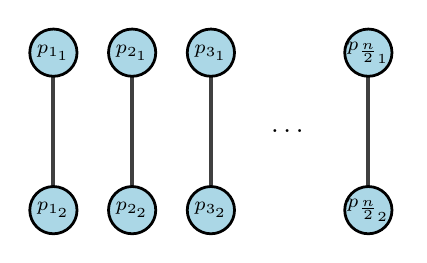
\begin{tikzpicture}
\Vertex[y=2,label=$p_{1_1}$]{A}
\Vertex[label=$p_{1_2}$]{B}
\Vertex[x=1,y=2,label=$p_{2_1}$]{C}
\Vertex[x=1,label=$p_{2_2}$]{D}
\Vertex[x=2,y=2,label=$p_{3_1}$]{E}
\Vertex[x=2,label=$p_{3_2}$]{F}
\Text[x=3,y=1]{\ldots}
\Vertex[x=4,y=2,label=$p_{\frac{n}{2}_1}$]{G}
\Vertex[x=4,label=$p_{\frac{n}{2}_2}$]{H}

\Edge(A)(B)
\Edge(C)(D)
\Edge(E)(F)
\Edge(G)(H)
\end{tikzpicture}
\end{center}

For each pair $p_i=(p_{i_1}, p_{i_2})$ in the $\frac{n}{2}$ pairs, where $1\le i \le \frac{n}{2}$, let us assign any distance $d_i$ between them such that we have not assigned that same distance on a different pair previously.

\begin{center}
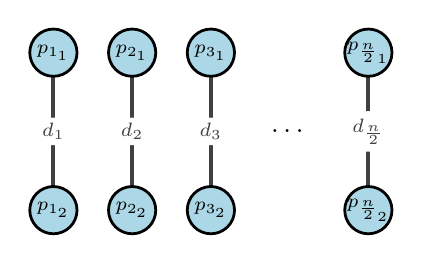
\begin{tikzpicture}
\Vertex[y=2,label=$p_{1_1}$]{A}
\Vertex[label=$p_{1_2}$]{B}
\Vertex[x=1,y=2,label=$p_{2_1}$]{C}
\Vertex[x=1,label=$p_{2_2}$]{D}
\Vertex[x=2,y=2,label=$p_{3_1}$]{E}
\Vertex[x=2,label=$p_{3_2}$]{F}
\Text[x=3,y=1]{\ldots}
\Vertex[x=4,y=2,label=$p_{\frac{n}{2}_1}$]{G}
\Vertex[x=4,label=$p_{\frac{n}{2}_2}$]{H}

\Edge[label=$d_1$](A)(B)
\Edge[label=$d_{2}$](C)(D)
\Edge[label=$d_{3}$](E)(F)
\Edge[label=$d_{\frac{n}{2}}$](G)(H)
\end{tikzpicture}
\end{center}

We know that for each pair $p_i=(p_{i_1}, p_{i_2})$ in the $\frac{n}{2}$ pairs, where $1\le i \le \frac{n}{2}$, if the assigned distance between $p_{i_1}$ and $p_{i_2}$ is the minimum distance between $p_{i_1}$ and $p_{j_1}$, $p_{i_1}$ and $p_{j_2}$, $p_{i_2}$ and $p_{j_1}$, $p_{i_2}$ and $p_{j_2}$, where $1\le j \le\frac{n}{2}$ and $i\neq j$, then $p_{i_1}$ and $p_{i_2}$ will send messages to each other, and receive messages from each other.

Let $k$ be the number of remaining unassigned pairs, we can make the antecedent of the above conditional statement true by simply assigning the remaining unassigned pairs by any distance $e_i$, where $0\le i\le k$, such that $e_i$ is greater than the maximum distance in the $\frac{n}{2}$ pairs, and we have not assigned $e_i$ on a different pair previously.

\begin{center}
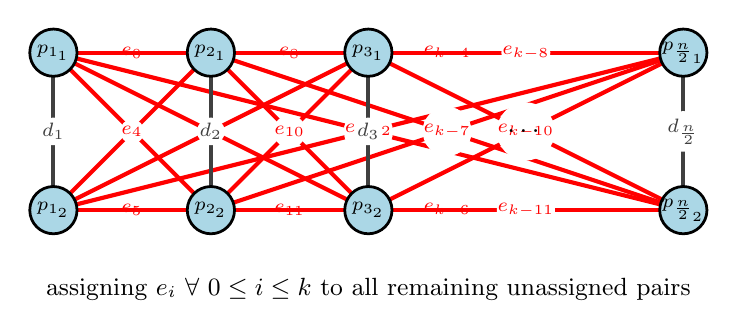
\begin{tikzpicture}
\Vertex[y=2,label=$p_{1_1}$]{A}
\Vertex[label=$p_{1_2}$]{B}
\Vertex[x=2,y=2,label=$p_{2_1}$]{C}
\Vertex[x=2,label=$p_{2_2}$]{D}
\Vertex[x=4,y=2,label=$p_{3_1}$]{E}
\Vertex[x=4,label=$p_{3_2}$]{F}
\Text[x=6,y=1]{\ldots}
\Vertex[x=8,y=2,label=$p_{\frac{n}{2}_1}$]{G}
\Vertex[x=8,label=$p_{\frac{n}{2}_2}$]{H}

\Edge[label=$e_0$,color=red](A)(C)
\Edge[label=$e_1$,color=red](A)(D)
\Edge[label=$e_2$,color=red](A)(E)
\Edge[label=$e_3$,color=red](A)(F)
\Edge[label=$e_k$,color=red](A)(G)
\Edge[label=$e_{k-1}$,color=red](A)(H)
\Edge[label=$e_4$,color=red](B)(C)
\Edge[label=$e_5$,color=red](B)(D)
\Edge[label=$e_6$,color=red](B)(E)
\Edge[label=$e_7$,color=red](B)(F)
\Edge[label=$e_{k-2}$,color=red](B)(G)
\Edge[label=$e_{k-3}$,color=red](B)(H)
\Edge[label=$e_8$,color=red](C)(E)
\Edge[label=$e_9$,color=red](C)(F)
\Edge[label=$e_{k-4}$,color=red](C)(G)
\Edge[label=$e_{k-5}$,color=red](C)(H)
\Edge[label=$e_{10}$,color=red](D)(E)
\Edge[label=$e_{11}$,color=red](D)(F)
\Edge[label=$e_{k-6}$,color=red](D)(H)
\Edge[label=$e_{k-7}$,color=red](D)(G)
\Edge[label=$e_{k-8}$,color=red](E)(G)
\Edge[label=$e_{k-9}$,color=red](E)(H)
\Edge[label=$e_{k-10}$,color=red](F)(G)
\Edge[label=$e_{k-11}$,color=red](F)(H)

\Edge[label=$d_1$](A)(B)
\Edge[label=$d_2$](C)(D)
\Edge[label=$d_3$](E)(F)
\Edge[label=$d_{\frac{n}{2}}$](G)(H)

\Text[x=4,y=-1,fontsize=\small]{assigning $e_i$ $\forall$ $0\le i\le k$ to all remaining unassigned pairs}
\end{tikzpicture}
\end{center}

By modus ponens, for all $p_i=(p_{i_1}, p_{i_2})$ in the $\frac{n}{2}$ pairs, where $1\le i \le \frac{n}{2}$, $p_{i_1}$ and $p_{i_2}$ will send messages to each other, and receive messages from each other. {\it[this is what we needed to show]}
\end{proof}

\subsubsection{Exercise 43}
Define a game as follows: You begin with an urn that contains a mixture of white and black balls, and during the game you have access to as many additional white and black balls as you might need. In each move you remove two balls from the urn without looking at their colors. If the balls
are the same color, you put in one black ball. If the balls are different colors, you put the white ball back into the urn and keep the black ball out. Because each move reduces the number of balls in the urn by one, the game will end with a single ball in the urn. If you know how many white balls and how many black balls are initially in the urn, can you predict the color of the ball at the end of the game? [This exercise is based on one described in “Why correctness must be a mathematical concern” by E. W. Dijkstra, www.cs.utexas.edu/users /EWD/transcriptions/EWD07xx/EWD720.html.]

(a)
Map out all possibilities for playing the game starting with two balls in the urn, then three balls, and then four balls. For each case keep track of the number of white and black balls you start with and the color of the ball at the
end of the game.

{\it Hint:}
\arrayrulecolor{cyan}
\begin{tabular}{|ccc|}
\hline
\multicolumn{3}{|c|}{\cy Two Balls} \\
\hline
WW & $\to$ & B \\
\hline
WB & $\to$ & W \\
\hline
BB & $\to$ & B \\
\hline
\end{tabular}
\begin{tabular}{|cc|cc|}
\hline
\multicolumn{4}{|c|}{\cy Summary} \\
\hline
\multicolumn{2}{|c|}{Start} & \multicolumn{2}{c|}{End} \\
\hline
W & B & W & B \\
\hline
2 & 0 & 0 & 1 \\
\hline
1 & 1 & 1 & 0 \\
\hline
0 & 2 & 0 & 1 \\
\hline
\end{tabular}

\begin{tabular}{|ccccc|c|}
\hline
\multicolumn{6}{|c|}{\cy Two Balls (2B)} \\
\hline
W & B & & W & B & Final Ball \\
\hline
2 & 0 & $\xRightarrow{WW}$ & 0 & 1 & B \\
\hline
1 & 1 & $\xRightarrow{WW}$ & 1 & 0 & W \\
\hline
0 & 2 & $\xRightarrow{WB}$ & 0 & 1 & B \\
\hline
\end{tabular}

\begin{tabular}{|ccccc|c|}
\hline
\multicolumn{6}{|c|}{\cy Three Balls (3B)} \\
\hline
W & B & & W & B & Final Ball (By 2B) \\
\hline
3 & 0 & $\xRightarrow{WW}$ & 1 & 1 & W \\
\hline
2 & 1 & $\xRightarrow{WW}$ & 0 & 2 & B \\
  &   & $\xRightarrow{WB}$ & 2 & 0 & B \\
\hline
1 & 2 & $\xRightarrow{WB}$ & 1 & 1 & W \\
  &   & $\xRightarrow{BB}$ & 1 & 1 & W \\
\hline
0 & 3 & $\xRightarrow{BB}$& 0 & 2 & B \\
\hline
\end{tabular}

\begin{tabular}{|ccccc|c|}
\hline
\multicolumn{6}{|c|}{\cy Four Balls} \\
\hline
W & B & & W & B & Final Ball (By 3B) \\
\hline
4 & 0 & $\xRightarrow{WW}$ & 2 & 1 & B \\
\hline
3 & 1 & $\xRightarrow{WW}$ & 1 & 2 & W \\
  &   & $\xRightarrow{WB}$ & 3 & 0 & W \\
\hline
2 & 2 & $\xRightarrow{WW}$ & 0 & 3 & B \\
  &   & $\xRightarrow{WB}$ & 2 & 1 & B \\
  &   & $\xRightarrow{BB}$ & 2 & 1 & B \\
\hline
1 & 3 & $\xRightarrow{WB}$ & 1 & 2 & W \\
  &   & $\xRightarrow{BB}$ & 1 & 2 & W \\
\hline
0 & 4 & $\xRightarrow{BB}$& 0 & 3 & B \\
\hline
\end{tabular}

\arrayrulecolor{black} % change it back!


(b)
Does the number of white balls seem to be predictive? Does the number of black balls seem to be predictive? Make a conjecture about the color of the ball at the end of the game given the numbers of white and black balls at the beginning.

{\it Hint:} In all three cases when the urn initially contains an odd number of white balls, there is one white ball in the urn at the end of the game, and when the urn initially contains an even number of white balls, there is one black ball (i.e., zero white balls) in the urn at the end of the game.

{\bf Conjecture: } For an urn that contains $n \ge 1$ mixture of white and black balls, if the number of white balls initially is even, then the remaining ball will be black after the game ends. Otherwise, it will be white.

(c)
Use mathematical induction to prove the conjecture you made in part (b).

\begin{proof}
Let $S(n)$ be the sentence: For an urn that contains $n \ge 1$ mixture of white and black balls, if the number of white balls initially is even, then the remaining ball will be black after the game ends. Otherwise, it will be white.

{\bf Show that $S(1)$ is true:} The urn contains one ball, this ball might be black or white.

Let us consider each cases.

{\bf Case 1: The ball is black.} Then the number of white balls initially is even (zero), the game ends as there is one ball in the urn, and the remaining ball is black, as expected.

{\bf Case 2: The ball is white.} Then the number of white balls initially is odd (one), the game ends as there is one ball in the urn, and the remaining ball is white, as expected.

For all cases, the remaining ball is consistent with S(1).

Hence, S(1) is true.

{\bf Show that $S(k) \implies S(k+1)$:} Let us first show that for any move, doing that move does not
    change the parity of the number of white balls in the urn. (*)

We know that in one move, the player randomly removes two balls. and adds one ball back in the urn with its color depending on the color of the two balls removed earlier.

Let us consider all possible color combinations for the removed balls.

{\bf Case 1: Both balls are black.} By the game rules, if player removes same color balls, then we need to put one black ball back in the urn. We did not change the number of white balls in the urn. Thus, we did not change the parity of white balls.

{\bf Case 2: Both balls are white.} By the game rules, if player removes same color balls, then we need to put one black ball back in the urn. We know that removing an even amount to any number, in this case the number of white balls in the urn, doesn't change the parity of that number. Thus, we did not change the parity of white balls.

{\bf Case 3: One ball is black, and the other is white.} By the game rules, if player removes different color balls, then we need to put one white ball back in the urn. We did not change the number of white balls in the urn. Thus, we did not change the parity of white balls.

In all cases, the parity of the number of white balls stayed the same after one move.

So * is true.

Now, to show that $S(k+1)$, let us first note that we are able to do at least one move in the game with $k+1$ balls. Because $k \ge1$, so $k+1 \ge2$, and we need at least two balls to do one move.

We know that $k+1$ balls can either have even or odd white balls.

Let us consider each case.

{\bf Case 1: There are even white balls in the $k+1$ balls.} After one move, we will end up with k balls, and we will end up with even white balls (By *). By $S(k)$, the remaining ball will be black.

{\bf Case 2: There are odd white balls in the $k+1$ balls.} After one move, we will end up with k balls, and we will end up with odd white balls (By *). By $S(k)$, the remaining ball will be white.

In all cases, the remaining ball is consistent with $S(k+1)$.

Hence, $S(k+1)$ is true.
\end{proof}

\subsubsection{Exercise 44}
Let $P(n)$ be the following sentence: Given any graph $G$ with $n$ vertices satisfying the condition that every vertex of $G$ has degree at most $M$, then the vertices of $G$ can be colored with at most $M + 1$ colors in such a way that no two adjacent vertices have the same color. Use mathematical induction to prove this statement is true for every integer $n \geq 1$.

{\it Hint:} Given a graph $G$ satisfying the given condition, form a new graph $G'$ by deleting one vertex $v$ of $G$ and all the edges that are incident on $v$. Then apply the inductive hypothesis to $G'$.

\begin{proof}
{\bf Show that $P(1)$ is true:} Given any graph $G$ with 1 vertex satisfying the given condition, we can color this vertex with only 1 color (which is $\leq M+1$) so that no two adjacent vertices have the same color (since there are no two adjacent vertices at all). So $P(1)$ is true.

{\bf Show that for any integer $k \geq 1$, if $P(k)$ is true then $P(k+1)$ is true:} Assume $P(k)$ is true, {\it [we want to prove $P(k+1)$ is true].} To prove $P(k+1)$ assume $G$ is any graph with $k+1$ vertices with degree at most $M$. {\it [We want to show that the vertices of $G$ can be colored with at most $M+1$ colors so that no two adjacent vertices have the same color.]}


Form a new graph $G'$ by deleting one vertex $v$ of $G$ and all the edges that are incident on $v$. Now $G'$ has $k$ vertices with degree at most $M$. By the inductive hypothesis we can color the vertices of $G'$ with at most $M+1$ colors so that no two adjacent vertices have the same color.

{\it ???}
\end{proof}

{\bf \cy In order for a proof by mathematical induction to be valid, the basis statement must be true for $n = a$ and the argument of the inductive step must be correct for every integer $k \geq a$. In 45 and 46 find the mistakes in the “proofs” by mathematical induction.}

\subsubsection{Exercise 45}
{\bf “Theorem:”} For any integer $n \geq 1$, all the numbers in a set of n numbers are equal to each other.

{\bf “Proof (by mathematical induction):} It is obviously true that all the numbers in a set consisting of just one number are equal to each other, so the basis step is true. For the inductive step, let $A = \{a_1, a_2, \ldots, a_k, a_{k+1}\}$ be any set of $k + 1$ numbers. Form two subsets each of size $k$:
\[
B = \{a_1, a_2, a_3, \ldots, a_k\} \text{ and } C = \{a_1, a_3, a_4, \ldots, a_{k+1}\}.
\]
($B$ consists of all the numbers in $A$ except $a_{k+1}$, and $C$ consists of all the numbers in $A$ except $a_2$.) By inductive hypothesis, all the numbers in $B$ equal $a_1$ and all the numbers in $C$ equal $a_1$ (since both sets have only $k$ numbers). But every number in $A$ is in $B$ or $C$, so all the numbers in $A$ equal $a_1$; hence all are equal to each other.”

\begin{proof}
The inductive step fails for going from $n = 1$ to $n = 2$,
because when $k = 1$,
\[
A = \{a_1, a_2\} \text{ and } B = \{a_1\}
\]
and no set $C$ can be defined to have the properties claimed for the $C$ in the proof. The reason is that $C = \{a_1\} = B$, and so an element of $A$, namely $a_2$, is
not in either $B$ or $C$.

Since the inductive step fails for going from $n = 1$ to $n = 2$, the truth of the following statement is never proved: “All the numbers in a set of two numbers are equal to each other.” This breaks the sequence of inductive steps, and so none of the statements for $n > 2$ is proved true either.

Here is an explanation for what happens in terms of the
domino analogy. The first domino is tipped backward (the basis step is proved). Also, if any domino from the second onward tips backward (the inductive step works or $n \geq 2$). In this case, however, when the first domino is tipped backward, it does not tip the second domino backward. So only the first domino falls down; the rest remain standing.
\end{proof}

\subsubsection{Exercise 46}
{\bf “Theorem:”} For every integer $n \geq 1$, $3^n - 2$ is even.

{\bf “Proof (by mathematical induction):} Suppose the theorem is true for an integer $k$, where $k \geq 1$. That is, suppose that $3^k - 2$ is even. We must show that $3^{k+1} - 2$ is even. Observe that $3^{k+1} - 2 = 3^k \cdot 3 - 2 = 3^k(1 + 2) - 2 = (3^k - 2) + 3^k \cdot 2$. Now $3^k - 2$ is even by inductive hypothesis and $3^k \cdot 2$ is even by inspection. Hence the sum of the two quantities is even (by Theorem 4.1.1). It follows that $3^{k+1} - 2$ is even, which is what we needed to show.”

{\it Hint:} Is the basis step true?

\begin{proof}
This proof starts at the inductive step, assuming $P(k)$ and proving $P(k+1)$. However, it does not prove the basis step. In fact, the basis step is false: when $n = 1$, $3^n - 2 = 3^1 - 2 = 1$ is odd.

(Even if the basis step were true, the proof is still incomplete as it's missing the basis step.)
\end{proof}

\subsection{Exercise Set 5.4}

\subsubsection{Exercise 1}
Suppose that $a_1, a_2, a_3, \ldots$ is a sequence defined
as follows:
\[
a_1 = 1, a_2 = 3, a_k = a_{k-2} + 2a_{k-1} \text{ for every integer $k \geq 3$.}
\]
Prove that $a_n$ is odd for every integer $n \geq 1$.

\begin{proof}
Let the property $P(n)$ be the sentence “$a_n$ is odd.”

{\bf Show that $P(1)$ and $P(2)$ are true:}

Observe that $a_1 = 1$ and $a_2 = 3$ and both 1 and 3 are odd. Thus $P(1)$ and $P(2)$ are true.

{\bf Show that for every integer $k \geq 2$, if $P(i)$ is true for each integer $i$ with $1 \leq i \leq k$, then $P(k + 1)$ is true:}

Let $k$ be any integer with $k \geq 2$, and suppose $a_i$ is odd for each integer $i$ with $1 \leq i \leq k$. {\it [This is the inductive hypothesis.]} We must show that $a_{k+1}$ is odd.

We know that $a_{k+1} = a_{k-1} + 2a_k$ by definition of $a_1, a_2, a_3, \ldots$. Moreover, $k - 1$ is less than $k + 1$ and is greater than or equal to 1 (because $k \geq 2$). Thus, by inductive hypothesis, $a_{k-1}$ is odd.

Also, every term of the sequence is an integer (being a sum of products of integers), and so $2a_k$ is even by definition of even.

It follows that $a_{k+1}$ is the sum of an odd integer and an even integer and hence is odd by Theorem 4.1.2 (Exercise 30, Section 4.1). {\it [This is what was to be shown.]}
\end{proof}

\subsubsection{Exercise 2}
Suppose that $b_1, b_2, b_3, \ldots$ is a sequence defined
as follows:
\[
b_1 = 4, b_2 = 12, b_k = b_{k-2} + b_{k-1} \text{ for every integer $k \geq 3$.}
\]
Prove that $b_n$ is divisible by 4 for every integer $n \geq 1$.

\begin{proof}
Let the property $P(n)$ be the sentence “$b_n$ is divisible by 4.”

{\bf Show that $P(1)$ and $P(2)$ are true:}

Observe that $b_1 = 4$ and $b_2 = 12$ and both 4 and 12 are divisible by 4. Thus $P(1)$ and $P(2)$ are true.

{\bf Show that for every integer $k \geq 2$, if $P(i)$ is true for each integer $i$ with $1 \leq i \leq k$, then $P(k + 1)$ is true:}

Let $k$ be any integer with $k \geq 2$, and suppose $b_i$ is divisible by 4 for each integer $i$ with $1 \leq i \leq k$. {\it [This is the inductive hypothesis.]} We must show that $b_{k+1}$ is divisible by 4.

We know that $b_{k+1} = b_{k-1} + b_k$ by definition of $b_1, b_2, b_3, \ldots$. Moreover, $k - 1$ and $k$ are both less than or equal to $k$ and are greater than or equal to 1 (because $k \geq 2$). Thus, by inductive hypothesis, $b_{k-1}$ and $b_k$ are divisible by 4. So by definition of divisible, $b_{k-1} = 4m$ and $b_k = 4n$ for some integers $m,n$.

It follows that $b_{k+1} = b_{k-1} + b_k = 4m + 4n = 4(m+n)$ is divisible by 4 because $m+n$ is an integer. {\it [This is what was to be shown.]}
\end{proof}

\subsubsection{Exercise 3}
Suppose that $c_0, c_1, c_2, \ldots$ is a sequence defined
as follows:
\[
c_0 = 2, c_1 = 2, c_2 = 6, c_k = 3c_{k-3} \text{ for every integer $k \geq 3$.}
\]
Prove that $c_n$ is even for every integer $n \geq 0$.

\begin{proof}
Let the property $P(n)$ be the sentence “$c_n$ is even.”

{\bf Show that $P(0), P(1)$ and $P(2)$ are true:}

Observe that $c_0 = 2, c_1 = 2$ and $c_2 = 6$ and both 2 and 6 are even. Thus $P(0), P(1)$ and $P(2)$ are true.

{\bf Show that for every integer $k \geq 2$, if $P(i)$ is true for each integer $i$ with $0 \leq i \leq k$, then $P(k + 1)$ is true:}

Let $k$ be any integer with $k \geq 2$, and suppose $c_i$ is even for each integer $i$ with $0 \leq i \leq k$. {\it [This is the inductive hypothesis.]} We must show that $c_{k+1}$ is even.

We have $c_{k+1} = 3c_{k-2}$ and $0 \leq k-2 \leq k$, therefore $c_{k-2}$ is even by inductive hypothesis. So $c_{k-2} = 2m$ for some integer $m$. Then $c_{k+1} = 3c_{k-2} = 3(2m) = 2(3m)$ where $3m$ is an integer. Thus $c_{k+1}$ is even. {\it [This is what was to be shown.]}
\end{proof}

\subsubsection{Exercise 4}
Suppose that $d_1, d_2, d_3, \ldots$ is a sequence defined
as follows:
\[
d_1 = \frac{9}{10}, d_2 = \frac{10}{11}, d_k = d_{k-1} \cdot d_{k-2} \text{ for every integer $k \geq 3$.}
\]
Prove that $0 < d_n \leq 1$ for every integer $n \geq 1$.

\begin{proof}
Let the property $P(n)$ be the inequality $d_n \leq 1$.

{\bf Show that $P(1)$ and $P(2)$ are true:}

Observe that $d_1 = 9/10$ and $d_2 = 10/11$ and both $9/10 \leq 1$ and $10 / 11 \leq 1$. Thus $P(1)$ and $P(2)$ are true.

{\bf Show that for every integer $k \geq 2$, if $P(i)$ is true for each integer $i$ with $1 \leq i \leq k$, then $P(k + 1)$ is true:}

Let $k$ be any integer with $k \geq 2$, and suppose $d_i \leq 1$ for each integer $i$ with $1 \leq i \leq k$. {\it [This is the inductive hypothesis.]} We must show that $d_{k+1} \leq 1$.

Now, by definition of $d_1, d_2, d_3, \ldots$, $d_{k+1} = d_k \cdot d_{k-1}$. Moreover $d_k \leq 1$ and $d_{k-1} \leq 1$ by inductive hypothesis because both $k - 1$ and $k$ are less than or equal to $k$.

Consequently, $d_{k+1} = d_k \cdot d_{k-1} \leq 1$ because if two positive numbers are each less than or equal to 1, then their product is less than or equal to 1.

{\it [To see why this is so, note that if $0 < a \leq 1$ and $0 < b \leq 1$, then multiplying $a \leq 1$ by $b$ gives $ab \leq b$, and since $b \leq 1$, then, by transitivity of order, $ab \leq 1$.]} Thus the inductive step has been proved.

{\it [Since we have proved both the basis step and the inductive step, we conclude that $d_n \leq 1$ for every integer $n \geq 1$.]}
\end{proof}

\subsubsection{Exercise 5}
Suppose that $e_0, e_1, e_2, \ldots$ is a sequence defined
as follows:
\[
e_0 = 12, e_1 = 29, e_k = 5e_{k-1} - 6e_{k-2} \text{ for every integer $k \geq 2$.}
\]
Prove that $e_n = 5 \cdot 3^n + 7 \cdot 2^n$ for every integer $n \geq 0$.

\begin{proof}
Let the property $P(n)$ be the equation $e_n = 5 \cdot 3^n + 7 \cdot 2^n$.

{\bf Show that $P(0)$ and $P(1)$ are true:}

We must show that $e_0 = 5 \cdot 3^0 + 7 \cdot 2^0$ and $e_1 = 5 \cdot 3^1 + 7 \cdot 2^1$.
The left-hand side of the first equation is 12 (by definition of $e_0, e_1, e_2, \ldots$), and its right-hand side is $5 \cdot 1 + 7 \cdot 1 = 12$ also.
The left-hand side of the second equation is 29 (by definition of $e_0, e_1, e_2, \ldots$), and its right-hand side is $5 \cdot 3 + 7 \cdot 2 = 29$ also.
Thus $P(0)$ and $P(1)$ are true.

{\bf Show that for every integer $k \geq 1$, if $P(i)$ is true for each integer $i$ with $0 \leq i \leq k$, then $P(k + 1)$ is also true:}

Let $k$ be any integer with $k \geq 1$ and suppose that $e_i = 5 \cdot 3^i + 7 \cdot 2^i$ for each integer $i$ with $0 \leq i \leq k$. {\it [This is the inductive hypothesis.]}
We must show that $e_{k+1} = 5 \cdot 3^{k+1} + 7 \cdot 2^{k+1}$. Now

\begin{center}
\begin{tabular}{rcll}
$\dps e_{k+1}$ & = & $\dps 5e_{k} - 6e_{k-1}$ & {\cy by definition of $e_0, e_1, e_2, \ldots$} \\
$\dps $ & = & $\dps 5(5 \cdot 3^k + 7 \cdot 2^k) - 6(5 \cdot 3^{k-1} + 7 \cdot 2^{k-1})$ & {\cy by inductive hypothesis} \\
$\dps $ & = & $\dps 25 \cdot 3^k + 35 \cdot 2^k - 30 \cdot 3^{k-1} - 42 \cdot 2^{k-1}$ & {\cy by distributing} \\
$\dps $ & = & $\dps 25 \cdot 3^k + 35 \cdot 2^k - 10 \cdot 3 \cdot 3^{k-1} - 21 \cdot 2 \cdot 2^{k-1}$ & {\cy by algebra} \\
$\dps $ & = & $\dps 25 \cdot 3^k + 35 \cdot 2^k - 10 \cdot 3^{k} - 21 \cdot 2^{k}$ & {\cy by laws of exponents} \\
$\dps $ & = & $\dps 15 \cdot 3^k + 14 \cdot 2^k$ & {\cy by combining like terms} \\
$\dps $ & = & $\dps 5 \cdot 3 \cdot 3^k + 7 \cdot 2 \cdot 2^k$ & {\cy by algebra} \\
$\dps $ & = & $\dps 5 \cdot 3^{k+1} + 7 \cdot 2^{k+1}$ & {\cy by laws of exponents} \\
\end{tabular}
\end{center}

{\it [as was to be shown].}
\end{proof}

\subsubsection{Exercise 6}
Suppose that $f_0, f_1, f_2, \ldots$ is a sequence defined
as follows:
\[
f_0 = 5, f_1 = 16, f_k = 7f_{k-1} - 10f_{k-2} \text{ for every integer $k \geq 2$.}
\]
Prove that $f_n = 3 \cdot 2^n + 2 \cdot 5^n$ for every integer $n \geq 0$.

\begin{proof}
Let the property $P(n)$ be the equation $f_n = 3 \cdot 2^n + 2 \cdot 5^n$.

{\bf Show that $P(0)$ and $P(1)$ are true:}

We must show that $f_0 = 3 \cdot 2^0 + 2 \cdot 5^0$ and $f_1 = 3 \cdot 2^1 + 2 \cdot 5^1$.
The left-hand side of the first equation is 5 (by definition of $f_0, f_1, f_2, \ldots$), and its right-hand side is $3 \cdot 2^0 + 2 \cdot 5^0 = 3 + 2 = 5$ also.
The left-hand side of the second equation is 16 (by definition of $f_0, f_1, f_2, \ldots$), and its right-hand side is $3 \cdot 2^1 + 2 \cdot 5^1 = 6 + 10 = 16$ also.
Thus $P(0)$ and $P(1)$ are true.

{\bf Show that for every integer $k \geq 1$, if $P(i)$ is true for each integer $i$ with $0 \leq i \leq k$, then $P(k + 1)$ is also true:}

Let $k$ be any integer with $k \geq 1$ and suppose that $f_i = 3 \cdot 2^i + 2 \cdot 5^i$ for each integer $i$ with $0 \leq i \leq k$. {\it [This is the inductive hypothesis.]}
We must show that $f_{k+1} = 3 \cdot 2^{k+1} + 2 \cdot 5^{k+1}$. Now

\begin{center}
\begin{tabular}{rcll}
$\dps f_{k+1}$ & = & $\dps 7f_{k} - 10f_{k-1}$ & {\cy by definition of $f_0, f_1, f_2, \ldots$} \\
$\dps $ & = & $\dps 7(3 \cdot 2^k + 2 \cdot 5^k) - 10(3 \cdot 2^{k-1} + 2 \cdot 5^{k-1})$ & {\cy by inductive hypothesis} \\
$\dps $ & = & $\dps 21 \cdot 2^k + 14 \cdot 5^k - 30 \cdot 2^{k-1} - 20 \cdot 5^{k-1}$ & {\cy by distributing} \\
$\dps $ & = & $\dps 21 \cdot 2^k + 14 \cdot 5^k - 15 \cdot 2 \cdot 2^{k-1} - 4 \cdot 5 \cdot 5^{k-1}$ & {\cy by algebra} \\
$\dps $ & = & $\dps 21 \cdot 2^k + 14 \cdot 5^k - 15 \cdot  2^{k} - 4 \cdot 5^{k}$ & {\cy by laws of exponents} \\
$\dps $ & = & $\dps 6 \cdot 2^k + 10 \cdot 5^k$ & {\cy by combining like terms} \\
$\dps $ & = & $\dps 3 \cdot 2 \cdot 2^k + 2 \cdot 5 \cdot 5^k$ & {\cy by algebra} \\
$\dps $ & = & $\dps 3 \cdot 2^{k+1} + 2 \cdot 5^{k+1}$ & {\cy by laws of exponents} \\
\end{tabular}
\end{center}

{\it [as was to be shown].}
\end{proof}

\subsubsection{Exercise 7}
Suppose that $g_1, g_2, g_3, \ldots$ is a sequence defined
as follows:
\[
g_1 = 3, g_2 = 5, g_k = 3g_{k-1} - 2g_{k-2} \text{ for every integer $k \geq 3$.}
\]
Prove that $g_n = 2^n + 1$ for every integer $n \geq 1$.

\begin{proof}
Let the property $P(n)$ be the equation $g_n = 2^n + 1$.

{\bf Show that $P(1)$ and $P(2)$ are true:}

We must show that $g_1 = 2^1 + 1$ and $g_2 = 2^2 + 1$.
The left-hand side of the first equation is 3 (by definition of $g_1, g_2, g_3, \ldots$), and its right-hand side is $2^1 + 1 = 2 + 1 = 3$ also.
The left-hand side of the second equation is 5 (by definition of $g_1, g_2, g_3, \ldots$), and its right-hand side is $2^2 + 1 = 4 + 1 = 5$ also.
Thus $P(1)$ and $P(2)$ are true.

{\bf Show that for every integer $k \geq 2$, if $P(i)$ is true for each integer $i$ with $1 \leq i \leq k$, then $P(k + 1)$ is also true:}

Let $k$ be any integer with $k \geq 2$ and suppose that $g_i = 2^i + 1$ for each integer $i$ with $1 \leq i \leq k$. {\it [This is the inductive hypothesis.]}
We must show that $g_{k+1} = 2^{k+1} + 1$. Now

\begin{center}
\begin{tabular}{rcll}
$\dps g_{k+1}$ & = & $\dps 3g_{k} - 2g_{k-1}$ & {\cy by definition of $g_1, g_2, g_3, \ldots$} \\
$\dps $ & = & $\dps 3(2^{k} + 1) - 2(2^{k-1} + 1)$ & {\cy by inductive hypothesis} \\
$\dps $ & = & $\dps 3 \cdot 2^k + 3 - 2^k - 2$ & {\cy by distributing} \\
$\dps $ & = & $\dps 2 \cdot 2^k + 1$ & {\cy by combining like terms} \\
$\dps $ & = & $\dps 2^{k+1} + 1$ & {\cy by laws of exponents} \\
\end{tabular}
\end{center}

{\it [as was to be shown].}
\end{proof}

\subsubsection{Exercise 8}
Suppose that $h_0, h_1, h_2, \ldots$ is a sequence defined
as follows:
\[
h_0 = 1, h_1 = 1, h_2 = 2, h_k = h_{k-1} + h_{k-2} + h_{k-3} \text{ for every integer $k \geq 3$.}
\]
(a)
Prove that $h_n \leq 3^n$ for every integer $n \geq 0$.

\begin{proof}
Let the property $P(n)$ be the inequality $h_n \leq 3^n$.

{\bf Show that $P(0), P(1)$ and $P(2)$ are true:}

We must show that $h_0 \leq 3^0, h_1 \leq 3^1$ and $h_2 \leq 3^2$.
The first inequality is $h_0 = 1 \leq 1 = 3^0$ which is true since $1 \leq 1$.
The second inequality is $h_1 = 1 \leq 3 = 3^1$ which is true since $1 \leq 3$.
The third inequality is $h_2 = 2 \leq 9 = 3^2$ which is true since $2 \leq 9$.
Thus $P(0), P(1)$ and $P(2)$ are true.

{\bf Show that for every integer $k \geq 2$, if $P(i)$ is true for each integer $i$ with $0 \leq i \leq k$, then $P(k + 1)$ is also true:}

Let $k$ be any integer with $k \geq 2$ and suppose that $h_i \leq 3^i$ for each integer $i$ with $0 \leq i \leq k$. {\it [This is the inductive hypothesis.]}
We must show that $h_{k+1} \leq 3^{k+1}$. Now

\begin{center}
\begin{tabular}{rcll}
$\dps h_{k+1}$ & = & $\dps h_{k} + h_{k-1} + h_{k-2}$ & {\cy by definition of $h_0, h_1, h_2, \ldots$} \\
$\dps $ & $\leq$ & $\dps 3^{k} + 3^{k-1} + 3^{k-2}$ & {\cy by inductive hypothesis} \\
$\dps $ & $\leq$ & $\dps 3^{k} + 3^{k} + 3^{k}$ & {\cy because $3^{k-1} \leq 3^k$ and $3^{k-2} \leq 3^k$} \\
$\dps $ & = & $\dps 3 \cdot 3^{k}$ & {\cy by combining like terms} \\
$\dps $ & = & $\dps 3^{k+1}$ & {\cy by laws of exponents} \\
\end{tabular}
\end{center}

{\it [as was to be shown].}
\end{proof}

(b)
Suppose that $s$ is any real number such that $s^3 \geq s^2 + s + 1$. (This implies that $2 > s > 1.83$.) Prove that $h_n \leq s^n$ for every integer $n \geq 2$.

\begin{proof}
Let the property $P(n)$ be the inequality $h_n \leq s^n$.

{\bf Show that $P(0), P(1)$ and $P(2)$ are true:}

We must show that $h_0 \leq s^0, h_1 \leq s^1$ and $h_2 \leq s^2$.
The first inequality is $h_0 = 1 \leq 1 = s^0$ which is true since $1 \leq 1$.
The second inequality is $h_1 = 1 \leq s^1$ which is true since $1 \leq 1.83 < s$.
The third inequality is $h_2 = 2 \leq s^2$ which is true since $2 \leq (1.83)^2 = 3.3489 < s^2$.
Thus $P(0), P(1)$ and $P(2)$ are true.

{\bf Show that for every integer $k \geq 2$, if $P(i)$ is true for each integer $i$ with $0 \leq i \leq k$, then $P(k + 1)$ is also true:}

Let $k$ be any integer with $k \geq 2$ and suppose that $h_i \leq s^i$ for each integer $i$ with $0 \leq i \leq k$. {\it [This is the inductive hypothesis.]}
We must show that $h_{k+1} \leq s^{k+1}$. Now

\begin{center}
\begin{tabular}{rcll}
$\dps h_{k+1}$ & = & $\dps h_{k} + h_{k-1} + h_{k-2}$ & {\cy by definition of $h_0, h_1, h_2, \ldots$} \\
$\dps $ & $\leq$ & $\dps s^{k} + s^{k-1} + s^{k-2}$ & {\cy by inductive hypothesis} \\
$\dps $ & $=$ & $\dps s^{k-2}(s^2 + s + 1)$ & {\cy by factoring $s^{k-2}$} \\
$\dps $ & $\leq$ & $\dps s^{k-2}(s^3)$ & {\cy by the fact $s^3 \geq s^2 + s + 1$} \\
$\dps $ & $=$ & $\dps s^{k+1}$ & {\cy by laws of exponents}
\end{tabular}
\end{center}

{\it [as was to be shown].}
\end{proof}

\subsubsection{Exercise 9}
Define a sequence $a_1, a_2, a_3, \ldots$ as follows:
\[
a_1 = 1, a_2 = 3, a_k = a_{k-1} + a_{k-2} \text{ for every integer $k \geq 3$.}
\]
(This sequence is known as the Lucas sequence.) Use strong
mathematical induction to prove that $a_n \leq (7/4)^n$ for every integer $n \geq 1$.

\begin{proof}
Let the property $P(n)$ be the inequality $a_n \leq (7/4)^n$.

{\bf Show that $P(1)$ and $P(2)$ are true:}

We must show that $a_1 \leq (7/4)^1$ and $a_2 \leq (7/4)^2$.
The first inequality is $a_1 = 1 \leq 7/4 = (7/4)^1$ which is true since $1 \leq 7/4$.
The second inequality is $a_2 = 3 \leq 3.0625 = 49 / 16 = (7/4)^2$ which is true since $3 \leq 3.0625$.
Thus $P(1)$ and $P(2)$ are true.

{\bf Show that for every integer $k \geq 2$, if $P(i)$ is true for each integer $i$ with $1 \leq i \leq k$, then $P(k + 1)$ is also true:}

Let $k$ be any integer with $k \geq 2$ and suppose that $a_i \leq (7/4)^i$ for each integer $i$ with $1 \leq i \leq k$. {\it [This is the inductive hypothesis.]}
We must show that $a_{k+1} \leq (7/4)^{k+1}$. Now

\begin{center}
\begin{tabular}{rcll}
$\dps a_{k+1}$ & = & $\dps a_{k} + a_{k-1}$ & {\cy by definition of $a_1, a_2, a_3, \ldots$} \\
$\dps $ & $\leq$ & $\dps (7/4)^{k} + (7/4)^{k-1}$ & {\cy by inductive hypothesis} \\
$\dps $ & $=$ & $\dps (7/4)^{k-1}(7/4 + 1)$ & {\cy by factoring $(7/4)^{k-1}$} \\
$\dps $ & $=$ & $\dps (7/4)^{k-1}(11/4)$ & {\cy by algebra} \\
$\dps $ & $\leq$ & $\dps (7/4)^{k-1}(49/16)$ & {\cy because $11/4 \leq 49/16$} \\
$\dps $ & $=$ & $\dps (7/4)^{k-1}(7/4)^2$ & {\cy by rewriting} \\
$\dps $ & $=$ & $\dps (7/4)^{k+1}$ & {\cy by laws of exponents}
\end{tabular}
\end{center}

{\it [as was to be shown].}
\end{proof}

\subsubsection{Exercise 10}
The introductory example solved with ordinary
mathematical induction in Section 5.3 can also be
solved using strong mathematical induction. Let $P(n)$
be “any $n$¢ can be obtained using a combination of
3¢ and 5¢ coins.” Use strong mathematical induction
to prove that $P(n)$ is true for every integer $n \geq 8$.

{\it Hint:} In the basis step, show that $P(8), P(9)$,
and $P(10)$ are all true. For the inductive step, note
that $k + 1 = [(k + 1) - 3] + 3$, and if $k \geq 10$, then
$(k + 1) - 3 \geq 8$.

\begin{proof}
{\bf Show that $P(8), P(9)$ and $P(10)$ are true:}
8¢ = 3¢ + 5¢ so $P(8)$ is true.
9¢ = 3¢ + 3¢ + 3¢ so $P(9)$ is true.
10¢ = 5¢ + 5¢ so $P(10)$ is true.

{\bf Show that for every $k \geq 10$, if $P(i)$ is true for every $i$ with $8 \leq i \leq k$ then $P(k+1)$ is true:}

Notice that $k - 2 \geq 8$, so by the inductive hypothesis, $(k-2)$¢ can be obtained using a combination of 3¢ and 5¢ coins.
Notice that $k + 1 = (k-2) + 3$. So $(k+1)$¢ can be obtained from $(k-2)$¢ by adding one more 3¢ coin.
Therefore $(k+1)$¢ can be obtained using a combination of 3¢ and 5¢ coins, {\it [as was to be shown.]}
\end{proof}

\subsubsection{Exercise 11}
You begin solving a jigsaw puzzle by finding two pieces that match and fitting them together.
Every subsequent step of the solution consists of fitting together two blocks, each of which is made up of one or more pieces that have previously been assembled.
Use strong mathematical induction to prove that for every integer $n \geq 1$, the number of steps required to put together all $n$ pieces of a jigsaw puzzle is $n - 1$.

\begin{proof}
Let the property $P(n)$ be the sentence ``A jigsaw puzzle consisting of $n$ pieces takes $n - 1$ steps to put together.''

{\bf Show that $P(1)$ is true:}
A jigsaw puzzle consisting of just one piece does not
take any steps to put together. Hence it is correct to say
that it takes zero steps to put together.

{\bf Show that for every integer $k \geq 1$, if $P(i)$ is true for each integer $i$ with $1 \leq i \leq k$, then $P(k + 1)$ is true:}

Let $k$ be any integer with $k \geq 1$ and suppose that for
each integer $i$ with $1 \leq i \leq k$, a jigsaw puzzle consisting of $i$ pieces takes $i - 1$ steps to put together. {\it [This is the inductive hypothesis.]}
We must show that a jigsaw puzzle consisting of $k + 1$ pieces takes $k$ steps to put together.

Consider assembling a jigsaw puzzle consisting of $k + 1$ pieces.
The last step involves fitting together two blocks. Suppose one of the blocks consists of $r$ pieces and the other consists of $s$ pieces. Then $r + s = k + 1$, and $1 \leq r \leq k$ and $1 \leq s \leq k$.
Thus, by the inductive hypothesis, the numbers of steps required to assemble the blocks are $r - 1$ and $s - 1$, respectively.
Then the total number of steps required to assemble the puzzle is $(r - 1) + (s - 1) + 1 = (r + s) - 1 = (k + 1) - 1 = k$ {\it [as was to be shown]}.
\end{proof}

\subsubsection{Exercise 12}
The sides of a circular track contain a sequence of $n$ cans of gasoline. For each integer $n \geq 1$, the total amount in the cans is sufficient to enable a certain car to make one complete circuit of the track.
In addition, all the gasoline could fit into the car’s gas tank at one time.
Use mathematical induction to prove that it is possible to find an initial location for placing the car so that it will be able to traverse the entire track by using the various amounts of gasoline in the cans that it encounters along the way.

{\it Hint:} For any collection of cans, at least one must
contain enough gasoline to enable the car to get to the
next can. (Why?)
Imagine taking all the gasoline from that can and pouring it into the can that immediately proceeds it in the direction of travel around the track.
{\it (I think ``precedes'' here is a typo in the book, I think they meant ``proceeds'' so I changed it.)}

\begin{proof}
Let $P(n)$ be the statement: ``It is possible to find an initial location for placing the car so that it will be able to traverse the entire track by using the various amounts of gasoline in the $n$ cans that it encounters along the way.''

{\bf Show that $P(1)$ is true:} In this case there is only one gasoline can. Let the initial location for the car to be this can. By the given assumption in the problem statement, the total amount in this can is sufficient to enable the car to make one complete circuit of the track. Therefore $P(1)$ is true.

{\bf Show that for any integer $k \geq 1$, if $P(k)$ is true then $P(k+1)$ is true:}

Assume $k \geq 1$ is any integer and assume $P(k)$ is true. Assume we are considering a circuit with $k+1$ gasoline cans. For convenience, label them $c_1, c_2, \ldots, c_{k+1}$ in the direction of the car's movement, and label their gasoline amounts as $g_1, g_2, \ldots, g_{k+1}$ respectively.

So the problem tells us that $g_1 + g_2 + \ldots + g_{k+1}$ is enough to allow the car make one complete track around the circuit.

{\bf Claim:} For any collection of cans, at least one must
contain enough gasoline to enable the car to get to the
next can.

{\it Proof of Claim.} Argue by contradiction and assume that no can contains enough gasoline to enable the car to get to the next can. Then the total amount in the cans is insufficient to enable the car to make one complete circuit, which is a contradiction to the fact given in the problem.

By the Claim, there exists a can, let's say $c_1$, that contains enough gasoline $g_1$ to reach the next can $c_2$ in the direction of movement.

Consider the circuit with $k$ gasoline cans obtained from the current track by combining the gasoline in $c_1$ and $c_2$ into $c_1$. This is a circuit with $k$ gasoline cans: we got rid of $c_2$ and now $c_1$ contains gasoline in the amount of $g_1 + g_2$. So the cans and their gasoline amounts are: $c_1: g_1 + g_2, c_3: g_3, c_4: g_4, \ldots, c_{k+1}: g_{k+1}$.

By the inductive hypothesis, there is an initial location in this $k$ can circuit, say at can $c_i$, that allows the car to make one complete track around this circuit.

Now we want to show that the same starting point, $c_i$, also works for our $k+1$ can circuit.

Let the car start at $c_i$. Then the car is able to travel to $c_1$ because the cans from $c_i$ up to $c_1$ have enough gasoline to allow the car to reach $c_1$ (by the inductive hypothesis). Some of this gasoline might be left over. When the car reaches $c_1$, say the remaining gasoline in the tank is $g$.  From this point on, we will talk about the two different circuit runs in parallel.

In the $k$ can circuit, now the car fuels up at can $c_1$ and receives $g_1 + g_2$ amount of gasoline. So $g + (g_1 + g_2)$ is enough to reach from $c_1$ to the next can, which is $c_3$ (by the inductive hypothesis).

To explain this a little bit better, say the exact amount of gasoline required to go from $c_1$ to $c_2$ is $G_1$, and the exact amount of gasoline required to go from $c_2$ to $c_3$ is $G_2$. So by the paragraph above, $g + g_1 + g_2 \geq G_1 + G_2$. And then the car reaches $c_3$ with $g + g_1 + g_2 - G_1 - G_2$ left in the tank, which is enough to complete the circuit back to $c_i$ (by the inductive hypothesis).

In the $k+1$ can circuit, now the car fuels up at can $c_1$ and receives $g_1$ amount of gasoline. Now there is $g + g_1$ in the tank. We know that $g_1$ is enough to go from $c_1$ to $c_2$ (by the property of $c_1$), so $g_1 \geq G_1$. Therefore the car reaches $c_2$ no problem, because $g + g_1 \geq G_1$. (Notice that if $g_1 \geq G_1$ weren't true, then the car would have to rely on the previous leftover $g$ to make up for the difference to reach $c_2$, which might not have been enough, since $g$ might be 0.)

Continuing on the $k+1$ circuit: when the car reaches $c_2$ there is $g + g_1 - G_1$ left in the tank. Now the car fuels up at $c_2$ and receives $g_2$ from $c_2$, so there is $g + g_1 - G_1 + g_2$ in the tank.

From the $k$ can circuit we know $g + g_1 + g_2 \geq G_1 + G_2$ which implies $g + g_1 + g_2 - G_1 \geq G_2$. The left hand side is the amount the tank has at $c_2$ in the $k+1$ can circuit. So this amount $g + g_1 + g_2 - G_1$ is enough from $c_2$ to reach $c_3$.

When the car reaches $c_3$ in the $k+1$ can circuit, there is $g + g_1 + g_2 - G_1 - G_2$ left in the tank, which is exactly the same as the $k$ can circuit, so it's enough to complete the track back to $c_i$.

This proves $P(k+1)$, {\it [as was to be shown.]}
\end{proof}

\subsubsection{Exercise 13}
Use strong mathematical induction to prove the existence part of the unique factorization of integers theorem (Theorem 4.4.5). In other words, prove that every integer greater than 1 is either a prime number or a product of prime numbers.

\begin{proof}
{\it Sketch of proof:} Given any integer $k > 1$, either $k$ is prime or $k$ is a product of two smaller positive integers, each greater than 1.
In the former case, the property is true.
In the latter case, the inductive hypothesis ensures that both factors of $k$ are products of primes and hence that $k$ is also a product of primes.

Let the property $P(n)$ be: ``There exist a positive integer $k$, distinct prime numbers $p_1, p_2, \ldots, p_k$, and positive integers $e_1, e_2, \ldots, e_k$ such that $n = p_1^{e_1} p_2^{e_2} p_3^{e_3} \cdots p_k^{e_k}$.''

{\bf Show that $P(2)$ is true:} We have $2 = 2^{1}$ so we can choose $k = 1$, $p_1 = 2$ and $e_1 = 1$. So $P(2)$ is true.

{\bf Show that for any integer $n > 1$ if $P(i)$ is true for all integers $i$ with $1 < i \leq n$ then $P(n+1)$ is true:}

Assume $n > 1$ is any integer and assume that for every integer $i$ with $1 < i \leq n$ there exist a positive integer $k_i$, distinct prime numbers $p_{1_i}, p_{2_i}, \ldots, p_{k_i}$ and positive integers $e_{1_i}, e_{2_i}, \ldots, e_{k_i}$ such that $i = p_{1_i}^{e_{1_i}} p_{2_i}^{e_{2_i}} p_{3_i}^{e_{3_i}} \cdots p_{k_i}^{e_{k_i}}$.

{\it [We want to show that there exist a positive integer $k$, distinct prime numbers $p_1, \ldots, p_k$, and positive integers $e_1, e_2, \ldots, e_k$ such that $n+1 = p_1^{e_1} p_2^{e_2} p_3^{e_3} \cdots p_k^{e_k}$.]}

{\bf Case 1: $n+1$ is prime.} Then $n + 1 = (n+1)^1$ so we can take $k = 1, p_1 = n+1, e_1 = 1$ which proves $P(n+1)$ is true.

{\bf Case 2: $n+1$ is composite.} By definition of composite $n+1 = ab$ for integers $a,b$ with $1 < a < n+1$ and $1 < b < n+1$.

By the inductive hypothesis $a = q_1^{f_1} q_2^{f_2} \cdots q_x^{f_x}$ and $b = r_1^{g_1} r_2^{g_2} \cdots r_y^{g_y}$ for some positive integers $x, y, f_1, \ldots, f_x, g_1, \ldots, g_y$ and some primes $q_1, \ldots, q_x, r_1, \ldots, r_y$. The primes $q_1, \ldots, q_x$ are distinct among themselves, and the primes $r_1, \ldots, r_y$ are distinct among themselves.

Then $n+1 = ab = q_1^{f_1} q_2^{f_2} \cdots q_x^{f_x} \cdot r_1^{g_1} r_2^{g_2} \cdots r_y^{g_y}$.

Now some of the primes $q_i$ might be among the primes $r_j$. If so, we can combine the powers in this product. For example if $q_i = r_j$ then we can let $s_i = q_i, h_i = f_i + g_j$ and combine the product $q_i^{f_i} \cdot r_j^{g_j} = s_i^{f_i + g_j} = s_i^{h_i}$.

This way, we obtain distinct primes $s_1, \ldots, s_z$ for some positive integer $z$, and positive integers $h_1, \ldots, h_z$ such that
\[
n+1 = ab = s_1^{h_1} \cdots s_z^{h_z}
\]
which proves $P(n+1)$, {\it [as was to be shown.]}
\end{proof}

\subsubsection{Exercise 14}
Any product of two or more integers is a result of successive multiplications of two integers at a time. For instance, here are a few of the ways in which $a_1, a_2, a_3, a_4$ might be computed: $(a_1 a_2)(a_3 a_4)$ or $((a_1 a_2) a_3) a_4)$ or $a_1((a_2 a_3) a_4)$. Use strong mathematical induction to prove that any product of two or more odd integers is odd.

\begin{proof}
Let the property $P(n)$ be the sentence “Any product of $n$ odd integers is odd.”

{\bf Show that $P(1)$ and $P(2)$ are true:}
$P(1)$ is true because any product of one odd integer is odd.
$P(2)$ is true because any product of two odd integers is odd (Exercise 20, Section 4.2).

{\bf Show that for every integer $k \geq 1$, if $P(i)$ is true for each integer $i$ with $1 \leq i \leq k$ then $P(k + 1)$ is true:}

Let $k$ be any integer with $k \geq 1$, and suppose that
for each integer $i$ with $1 \leq i \leq k$, any product
of $i$ odd integers is odd. {\it [Inductive hypothesis]}

Consider any product $M$ of $k + 1$ odd integers.
Some multiplication is the final one that is used to obtain $M$.
Thus, there are integers $A$ and $B$ such that $M = AB$,
and each of $A$ and $B$ is a product of between 1 and $k$
odd integers.
(For instance, if $M = ((a_1a_2)a_3)a_4$, then $A = (a_1a_2)a_3$ and $B = a_4$.)
By inductive hypothesis, each of $A$ and $B$ is odd, and,
as in the basis step, we know that any product of two odd
integers is odd. Hence $M = AB$ is odd.
\end{proof}

\subsubsection{Exercise 15}
Define the “sum” of one integer to be that integer, and use strong mathematical induction to prove that for every integer $n \geq 1$, any sum of $n$ even integers is even.

\begin{proof}
Let $P(n)$ be the statement ``any sum of $n$ even integers is even.''

{\bf Show that $P(1)$ is true:} The sum of one even integer is equal to itself, which is even. Thus $P(1)$ is true.

{\bf Show that for every integer $k \geq 1$ if $P(i)$ is true for all integers $i$ with $1 \leq i \leq k$ then $P(k+1)$ is true:}

Assume $k \geq 1$ is an integer such that any sum of $i$ even integers is even, for any integer $i$ with $1 \leq i \leq k$. {\it [We want to show that any sum of $k+1$ even integers is even.]}

Consider any sum $S$ of $k+1$ even integers.
Some addition is the final one that is used to obtain $S$.
Thus, there are integers $A$ and $B$ such that $S = A + B$,
and each of $A$ and $B$ is a sum of between 1 and $k$
even integers.
(For instance, if $S = ((a_1 + a_2) + a_3) + a_4$, then $A = (a_1 + a_2) + a_3$ and $B = a_4$.)
By inductive hypothesis, each of $A$ and $B$ is even, and,
we know that any sum of two even integers is even. Hence $S = A + B$ is even, {\it [as was to be shown.]}
\end{proof}

\subsubsection{Exercise 16}
Use strong mathematical induction to prove that for every integer $n \geq 2$, if $n$ is even, then any sum of $n$ odd integers is even, and if $n$ is odd, then any sum of $n$ odd integers is odd.

{\it Hint:} Let the property $P(n)$ be the sentence “If
$n$ is even, then any sum of $n$ odd integers is even,
and if $n$ is odd, then any sum of $n$ odd integers is odd.”
For the inductive step, consider any sum $S$ of $k + 1$ odd integers.
Some addition is the final one that is used to obtain $S$.
Thus, there are integers $A$ and $B$ such that $S = A + B$,
and $A$ is a sum of $r$ odd integers
and $B$ is a sum of $(k + 1) - r$ odd integers.
Consider the two cases where $k + 1$ is even and $k + 1$ is
odd, and for each case consider the two subcases where $r$
is even and where $r$ is odd.

\begin{proof}
(following the Hint)

{\bf Show that $P(2)$ is true:} 2 is even, so we need to show that any sum of 2 odd integers is even. Assume $m, n$ are two odd integers.
{\it [We want to show $m+n$ is even.]}
By definition of odd $m = 2a+1$ and $n = 2b+1$ for some integers $a,b$.
Then $m+n = 2a+1 + 2b + 1 = 2(a+b+1)$ where $a+b+1$ is an integer (because $a$ and $b$ are integers).
So by definition of even, $m+n$ is even. This proves $P(2)$.

{\bf Show that for every integer $k \geq 2$, if $P(i)$ is true for all integers $i$ with $2 \leq i \leq k$ then $P(k+1)$ is true:}

Assume $k \geq 2$ is any integer such that for all $i$ with $2 \leq i \leq k$, if $i$ is even then any sum of $i$ odd integers is even, and if $i$ is odd then any sum of $i$ odd integers is odd.

{\it [We want to show that if $k+1$ is even, then any sum of $k+1$ odd integers is even, and if $k+1$ is odd, then any sum of $k+1$ odd integers is odd.]}

Consider any sum $S$ of $k+1$ odd integers.
Some addition is the final one that is used to obtain $S$.
Thus, there are integers $A$ and $B$ such that $S = A + B$,
$A$ is a sum of $r$ odd integers and $B$ is a sum of $(k + 1) - r$ odd integers.

{\bf Case 1: $k+1$ is even.} {\it [We want to show that $S$ is even.]}

{\bf Subcase 1.1: $r$ is even.}
Then $(k+1) - r$ is even. So both $A$ and $B$ are sums of an even number of odd integers.
By inductive hypothesis $A$ and $B$ are both even.
Therefore $S = A + B$ is even (a sum of two even integers),
{\it [as was to be shown.]}

{\bf Subcase 1.2: $r$ is odd.}
Then $(k+1) - r$ is odd. So both $A$ and $B$ are sums of an odd number of odd integers.
By inductive hypothesis $A$ and $B$ are both odd.
Therefore $S = A + B$ is even (a sum of two odd integers),
{\it [as was to be shown.]}

{\bf Case 2: $k+1$ is odd.} {\it [We want to show that $S$ is odd.]}

{\bf Subcase 2.1: $r$ is even.}
Then $(k+1) - r$ is odd.
So $A$ is a sum of an even number of odd integers, and
$B$ is a sum of an odd number of odd integers.
By inductive hypothesis $A$ is even and $B$ is odd.
Therefore $S = A + B$ is odd
(a sum of one even and one odd integers),
{\it [as was to be shown.]}

{\bf Subcase 2.2: $r$ is odd.}
Then $(k+1) - r$ is even.
So $A$ is a sum of an odd number of odd integers, and
$B$ is a sum of an even number of odd integers.
By inductive hypothesis $A$ is odd and $B$ is even.
Therefore $S = A + B$ is odd
(a sum of one odd and one even integers),
{\it [as was to be shown.]}
\end{proof}

\subsubsection{Exercise 17}
Compute $4^1, 4^2, 4^3, 4^4, 4^5, 4^6, 4^7$, and $4^8$.
Make a conjecture about the units digit of $4^n$ where $n$ is a positive integer.
Use strong mathematical induction to prove your conjecture.

\begin{proof}
$4^1 = 4, 4^2 = 16, 4^3 = 64, 4^4 = 256, 4^5 = 1024, 4^6 = 4096, 4^7 = 16384, 4^8 = 65536$.

{\it Conjecture:}
The units digit of $4^n$ equals 4 if $n$ is odd and equals 6 if $n$ is even,
for all $n \geq 1$.

\underline{Proof by strong mathematical induction:}
Let $P(n)$ be the statement:
``The units digit of $4^n$ is 4 if $n$ is odd, 6 if $n$ is even.''

{\bf Show that $P(1)$ and $P(2)$ are true:}
When $n = 1$, $4^n = 4^1 = 4$, so the units digit is 4.
When $n = 2$, $4^n = 4^2 = 16$, so the units digit is 6.
Therefore $P(1)$ and $P(2)$ are true.

{\bf Show that for all integers $k \geq 2$, if $P(i)$ is true for all integers $i$ with $1 \leq i \leq k$ then $P(k+1)$ is true:}

Let $k$ by any integer with $k \geq 2$, and suppose that for each integer $i$
with $1 \leq i \leq k$, the units digit of $4^i$ equals 4 if $i$ is odd and
equals 6 if $i$ is even. {\it [Inductive hypothesis]}
We must show that the units digit of $4^{k+1}$ equals 4
if $k + 1$ is odd and equals 6 if $k + 1$ is even.

{\bf Case 1 ($k + 1$ is odd):} In this case, $k$ is even,
and so, by inductive hypothesis, the units digits of $4^k$ is 6.
Thus $4^k = 10q + 6$ for some nonnegative integer $q$. It follows that
$4^{k+1} = 4^k \cdot 4 = (10q + 6) \cdot 4 = 40q + 24 = 10(4q + 2) + 4$.
Thus, the units digit of $4^{k+1}$ is 4.

{\bf Case 2 ($k + 1$ is even):} In this case, $k$ is odd,
and so, by inductive hypothesis, the units digits of $4^k$ is 4.
Thus $4^k = 10q + 4$ for some nonnegative integer $q$. It follows that
$4^{k+1} = 4^k \cdot 4 = (10q + 4) \cdot 4 = 40q + 16 = 10(4q + 1) + 6$.
Thus, the units digit of $4^{k+1}$ is 6.

{\bf\it Conclusion:} Because cases 1 and 2 are the only
possibilities and $4^{k+1}$ has one of the required forms
in each case, we have shown that $P(k + 1)$ is true.
\end{proof}

\subsubsection{Exercise 18}
Compute $9^0, 9^1, 9^2, 9^3, 9^4$, and $9^5$. Make a conjecture about the units digit of $9^n$ where $n$ is a positive integer. Use strong mathematical induction to prove your conjecture.

\begin{proof}
$9^0 = 1, 9^1 = 9, 9^2 = 81, 9^3 = 729, 9^4 = 6561, 9^5 = 59049$.

{\it Conjecture:}
The units digit of $9^n$ equals 9 if $n$ is odd and equals 1 if $n$ is even, for $n \geq 0$.

\underline{Proof by strong mathematical induction:}
Let $P(n)$ be the statement:
``The units digit of $9^n$ is 9 if $n$ is odd, 1 if $n$ is even.''

{\bf Show that $P(0)$ and $P(1)$ are true:}
When $n = 0$, $9^n = 9^0 = 1$, so the units digit is 1.
When $n = 1$, $9^n = 9^1 = 9$, so the units digit is 9.
Therefore $P(0)$ and $P(1)$ are true.

{\bf Show that for all integers $k \geq 1$, if $P(i)$ is true for all integers $i$ with $0 \leq i \leq k$ then $P(k+1)$ is true:}

Let $k$ by any integer with $k \geq 1$, and suppose that for each integer $i$
with $0 \leq i \leq k$, the units digit of $9^i$ equals 9 if $i$ is odd and
equals 1 if $i$ is even. {\it [Inductive hypothesis]}
We must show that the units digit of $9^{k+1}$ equals 9
if $k + 1$ is odd and equals 1 if $k + 1$ is even.

{\bf Case 1 ($k + 1$ is odd):} In this case, $k$ is even, and so, by inductive
hypothesis, the units digits of $9^k$ is 1.
Thus $9^k = 10q + 1$ for some nonnegative integer $q$. It follows that
$9^{k+1} = 9^k \cdot 9 = (10q + 1) \cdot 9 = 90q + 9 = 10(9q) + 9$.
Thus, the units digit of $9^{k+1}$ is 9.

{\bf Case 2 ($k + 1$ is even):} In this case, $k$ is odd, and so, by inductive
hypothesis, the units digits of $9^k$ is 9.
Thus $9^k = 10q + 9$ for some nonnegative integer $q$. It follows that
$9^{k+1} = 9^k \cdot 9 = (10q + 9) \cdot 9 = 90q + 81 = 10(9q + 8) + 1$.
Thus, the units digit of $9^{k+1}$ is 1.

{\bf\it Conclusion:} Because cases 1 and 2 are the only
possibilities and $9^{k+1}$ has one of the required forms
in each case, we have shown that $P(k + 1)$ is true.
\end{proof}

\subsubsection{Exercise 19}
Suppose that $a_1, a_2, a_3, \ldots$ is a sequence defined as follows:
\[
a_1 = 1, a_k = 2 \cdot a_{\floor{k/2}} \text{ for every integer } k \geq 2.
\]
Prove that $a_n \leq n$ for each integer $n \geq 1$.

\begin{proof}
Let the property $P(n)$ be the inequality $a_n \leq n$. {\cy $\from P(n)$}

We will show that $P(n)$ is true for each integer $n \geq 1$.

{\bf Show that $P(1)$ is true:} $a_1 = 1$ and $1 \leq 1$. So $P(1)$ is true.

{\bf Show that for every integer $k \geq 1$, if $P(i)$ is true for each integer
$i$ from 1 through $k$, then $P(k + 1)$ is true:} Let $k$ be any integer with
$k \geq 1$, and suppose that $a_i \leq i$ for each integer $i$ with
$1 \leq i \leq k$. {\cy $\from$ inductive hypothesis}

We must show that $a_{k+1} \leq k + 1$. Now

\begin{center}
\begin{tabular}{rcll}
$\dps a_{k+1}$ & = & $\dps 2 \cdot a_{\floor{(k+1)/2}}$ & {\cy by definition of $a_1, a_2, a_3, \ldots$} \\
$\dps $ & $\leq$ & $\dps 2 \cdot \floor{(k+1)/2}$ & {\cy by inductive hypothesis} \\
$\dps $ & $=$ & $\dps
\left\{
\begin{array}{lr}
2((k+1)/2) & \text{if $k$ is odd} \\
2(k/2) & \text{if $k$ is even} \\
\end{array}
\right.$ & {\cy by definition of floor} \\
$\dps $ & $=$ & $\dps
\left\{
\begin{array}{lr}
k+1 & \text{if $k$ is odd} \\
k & \text{if $k$ is even} \\
\end{array}
\right.$ & {\cy by algebra} \\
$\dps $ & $\leq$ & $\dps k+1$ & {\cy because $k \leq k+1$}
\end{tabular}
\end{center}

Thus $a_{k+1} \leq k + 1$ {\it [as was to be shown].}
\end{proof}

\subsubsection{Exercise 20}
Suppose that $b_1, b_2, b_3, \ldots$ is a sequence defined as follows:
\[
b_1 = 0, b_2 = 3, b_k = 5 \cdot b_{\floor{k/2}} + 6 \text{ for every integer } k \geq 3.
\]
Prove that $b_n$ is divisible by 3 for each integer $n \geq 1$.

\begin{proof}
Let the property $P(n)$ be the statement $3 \mid b_n$. {\cy $\from P(n)$}

We will show that $P(n)$ is true for each integer $n \geq 1$.

{\bf Show that $P(1)$ and $P(2)$ are true:}
$b_1 = 0 = 3 \cdot 0$ and $b_2 = 3 = 3 \cdot 1$.
So $3 \mid b_1$ and $3 \mid b_2$.
So $P(1)$ and $P(2)$ are true.

{\bf Show that for every integer $k \geq 2$, if $P(i)$ is
true for each integer $i$ from 1 through $k$, then $P(k + 1)$ is true:}

Let $k$ be any integer with $k \geq 2$, and suppose that
$3 \mid b_i$ for each integer $i$ with $1 \leq i \leq k$.
{\cy $\from$ inductive hypothesis}

We must show that $3 \mid b_{k+1}$.

{\bf Case 1: $k$ is even.}
Then $k = 2i$ for some integer $i$ with $1 \leq i < k$, and
$\dps \floor{(k+1)/2} = \floor{(2i+1)/2} = \floor{i+1/2} = i$.
By the inductive hypothesis, $3 \mid b_i$. So $b_i = 3m$ for some integer $m$. Then
\[
b_{k+1} = 5 \cdot b_{\floor{(k + 1)/2}} + 6 = 5 \cdot b_i + 6 = 5 \cdot (3m) + 6 = 3(5m + 2)
\]
so by definition of divides, $3 \mid b_{k+1}$, {\it [as was to be shown.]}

{\bf Case 2: $k$ is odd.}
Then $k = 2i + 1$ for some integer $i$ with $1 \leq i < k$,
and $\dps \floor{(k + 1)/2} = \floor{(2i + 1 + 1)/2} = \floor{(2i + 2)/2} = \floor{i+1}= i+1$.
Note that $i + 1 \leq k$.
By the inductive hypothesis, $3 \mid b_{i + 1}$. So $b_{i + 1} = 3m$ for some integer $m$. Then
\[
b_{k+1} = 5 \cdot b_{\floor{(k + 1)/2}} + 6 = 5 \cdot b_{i + 1} + 6 = 5 \cdot (3m) + 6 = 3(5m + 2)
\]
so by definition of divides, $3 \mid b_{k+1}$, {\it [as was to be shown.]}
\end{proof}

\subsubsection{Exercise 21}
Suppose that $c_0, c_1, c_2, c_3, \ldots$ is a sequence defined as follows:
\[
c_0 = 1, c_1 = 1, c_k = c_{\floor{k/2}} + c_{\ceil{k/2}}  \text{ for every integer } k \geq 2.
\]
Prove that $c_n = n$ for each integer $n \geq 1$.

\begin{proof}
Let the property $P(n)$ be the equality $c_n = n$. {\cy $\from P(n)$}

We will show that $P(n)$ is true for each integer $n \geq 1$.

{\bf Show that $P(1)$ is true:}
$c_1 = 1$ so $P(1)$ is true.

{\bf Show that for every integer $k \geq 1$, if $P(i)$ is
true for each integer $i$ from 1 through $k$, then $P(k + 1)$ is true:}

Let $k$ be any integer with $k \geq 1$, and suppose that
$c_i = i$ for each integer $i$ with $1 \leq i \leq k$.
{\cy $\from$ inductive hypothesis}

We must show that $c_{k+1} = k+1$.

{\bf Case 1: $k$ is even.}
Then $k = 2i$ for some integer $i$ with $1 \leq i < k$. So:

$\dps \floor{(k+1)/2} = \floor{(2i+1)/2} = \floor{i+1/2} = i$, and

$\dps \ceil{(k+1)/2} = \ceil{(2i+1)/2} = \ceil{i+1/2} = i+1$.

Notice that $i + 1 \leq k$.

By the inductive hypothesis, $c_i = i$ and $c_{i+1} = i+1$. Then
\[
c_{k+1} = c_{\floor{(k+1)/2}} + c_{\ceil{(k+1)/2}} = c_i + c_{i+1} = i + (i+1) = 2i+1 = k+1,
\]
{\it [as was to be shown.]}

{\bf Case 2: $k$ is odd.}
Then $k = 2i + 1$ for some integer $i$ with $1 \leq i < k$. So:

$\dps \floor{(k + 1)/2} = \floor{(2i + 1 + 1)/2} = \floor{i + 1} = i + 1$, and

$\dps \ceil{(k + 1)/2} = \ceil{(2i + 1 + 1)/2} = \ceil{i + 1} = i+1$.

Notice that $i + 1 \leq k$.

By the inductive hypothesis $c_{i+1} = i+1$. Then
\[
c_{k + 1} = c_{\floor{(k+1)/2}} + c_{\ceil{(k+1)/2}} = c_{i + 1} + c_{i + 1} = (i+1) + (i+1) = 2i+2 = k+1,
\]
{\it [as was to be shown.]}
\end{proof}

\subsubsection{Exercise 22}
One version of the game NIM starts with two piles of
objects such as coins, stones, or matchsticks. In each turn
a player is required to remove from one to three objects
from one of the piles. The two players take turns doing
this until both piles are empty. The loser is the first
player who can’t make a move. Use strong mathematical
induction to show that if both piles contain the same
number of objects at the start of the game, the player who
goes second can always win.

\begin{proof}
Let $P(n)$ be the sentence
\begin{center}
In this version of NIM, if both piles initially contain $n$ objects, the player who goes second can always win.
\end{center}

We will prove that $P(n)$ is true for every integer $n \geq 0$.

{\bf Show that $P(0)$ is true:}

If neither pile contains any objects, the player who goes first automatically loses because of not being able to make a move. So the second player wins the game by default. Thus $P(0)$ is true.

{\bf Show that for every integer $k \geq 0$, if $P(i)$ is true for each integer $i$ from 1 through $k$, then $P(k + 1)$ is true:}

Let $k$ be any integer with $k \geq 0$, and suppose:
\begin{center}
In this version of NIM, for every integer $i$ with $0 \leq i \leq k$,
if both piles initially contain $i$ objects, the player who goes second can always win.
\end{center}
We must show that In this version of NIM, if both piles initially contain $k + 1$ objects, the player who goes second can always win. {\cy $\from P(k + 1)$}

So suppose both piles contain $k + 1$ objects, where $0 \leq i \leq k$, and
suppose the first player removes $r$ objects from pile \#1, where $1 \leq r \leq 3$.
If the second player removes $r$ objects from pile \#2, then both piles will
have the same number of objects, namely $(k + 1) - r$, and $(k + 1) - r \leq k$
because $r \geq 1$. Thus, by inductive hypothesis, the second player can win.
\end{proof}

\subsubsection{Exercise 23}
Define a game $G$ as follows: Begin with a pile of $n$ stones and 0 points. In the first move split the pile into
two possibly unequal sub-piles, multiply the number of stones in one sub-pile times the number of stones in the
other sub-pile, and add the product to your score. In the second move, split each of the newly created piles into a
pair of possibly unequal sub-piles, multiply the number of stones in each sub-pile times the number of stones in the
paired sub-pile, and add the new products to your score. Continue by successively splitting each newly created pile
of stones that has at least two stones into a pair of sub-piles, multiplying the number of stones in each sub-pile
times the number of stones in the paired sub-pile, and adding the new products to your score. The game $G$ ends
when no pile contains more than one stone.

(a)
Play $G$ starting with 10 stones and using the following initial moves. In move 1 split the pile of 10 stones into two sub-piles with 3 and 7 stones respectively, compute $3 \cdot 7 = 21$, and find that your score is 21. In move 2 split the pile of 3 stones into two sub-piles, with 1 and 2 stones respectively, and split the pile of 7 stones into two sub-piles, with 4 and 3 stones respectively, compute $1 \cdot 2 = 2$ and $4 \cdot 3 = 12$, and find that your score is $21 + 2 + 12 = 35$. In move 3 split the pile of 4 stones into two sub-piles, each with 2 stones, and split the pile of 3 stones into two sub-piles, with 1 and 2 stones respectively, and find your new score. Continue splitting piles and computing your score until no pile has more than one stone. Show your final score along with a record of the numbers of stones in the piles you created with your moves.

\begin{proof}
\begin{figure}[ht!]
\centering
\includegraphics[scale=0.6]{../images/5.4.23.a.png}
\end{figure}
\end{proof}

(b)
Play $G$ again starting with 10 stones, but use a different initial move from the one in part (a). Show your final score along with a record of the numbers of stones in the piles you created with your moves.

\begin{proof}
\[
\arrayrulecolor{cyan}
\begin{array}{|c|c|c|c|c|c|c|c|c|c|c|c|}
\hline
\multicolumn{10}{|c|}{10} & & \\
\hline
\multicolumn{2}{|c}{2} & \multicolumn{8}{|c|}{8} & 2 \cdot 8 & 16 \\
\hline
1 & 1 & \multicolumn{4}{c|}{4} & \multicolumn{4}{c|}{4} & 1 \cdot 1 + 4 \cdot 4 & 17 \\
\hline
 &  & \multicolumn{2}{c|}{2} & \multicolumn{2}{c|}{2} & \multicolumn{2}{c|}{2} & \multicolumn{2}{c|}{2} & 2 \cdot 2 + 2 \cdot 2 & 8 \\
\hline
 &  & 1 & 1 & 1 & 1 & 1 & 1 & 1 & 1 & 1 \cdot 1 + 1 \cdot 1 + 1 \cdot 1 + 1 \cdot 1 & 4 \\
\hline
\end{array}
\arrayrulecolor{black}
\]
{\bf TOTAL} 45
\end{proof}

(c)
Show that you can use strong mathematical induction to prove that for every integer $n \geq 1$, given the set-up of game $G$, no matter how you split the piles in the various moves, your final score is $n(n - 1)/2$. The basis step may look a little strange because a pile consisting of one stone cannot be split into any sub-piles. Another way to say this is that it can only be split into zero piles, and that gives an answer that agrees with the general formula for the final score.

\begin{proof}
Let $P(n)$ be the statement: ``No matter how you split the piles in the various moves, your final score is $n(n-1)/2$.''

{\bf Show that $P(1)$ is true:} A pile of 1 stone cannot be split, therefore the score is 0, and $1(1-1)/2 = 0$ also. So $P(1)$ is true.

{\bf Show that for any integer $k \geq 1$ if $P(i)$ is true for all integers $i$ with $1 \leq i \leq k$ then $P(k+1)$ is true:}

Assume $k \geq 1$ is an integer and assume that for all integers $i$ with $1 \leq i \leq k$, a game played with
starting $i$ stones, no matter how you split the piles in various moves, your final score is $i(i-1)/2$.

{\it [We want to show that in a game played with $k+1$ starting stones, no matter how you split the piles in
various moves, your final score is $(k+1)(k+2)/2$.]}

Starting with $k+1$ stones, there are $\dps \floor{\frac{k + 1}{2}}$ different ways to split the stones: 1 and $k$,
2 and $k-1$, 3 and $k-2, \ldots$, and $k/2$ and $k/2 + 1$ if $k+1$ is odd, $(k+1) / 2$ and $(k+1) / 2$ if $k+1$ is even.

In other words, the first move splits the stones into piles of $i$ and $(k+1) - i$ for some $1 \leq i \leq \floor{(k + 1) / 2}$.
The score of this first move is $i(k+1-i) = ki + i - i^2$.

Then the rest of the game consists of two sub-games with starting piles of $i$ and $(k+1)-i$. By the inductive
hypothesis, no matter how you split the stones in these sub-games, the final scores are
\[
\frac{i(i+1)}{2} = \frac{i^2 + i}{2}
\]
and $\dps \frac{(k+1-i)(k+1-i+1)}{2}$
\[
= \frac{(k+1-i)(k+2-i)}{2} = \frac{k^2 + 2k - ik + k + 2 - i - ik - 2i + i^2}{2}
\]
$\dps = \frac{k^2 + (3 - 2i)k + 2 - 3i + i^2}{2}$, respectively.

Then the total final score of the $k+1$ stone game is:
\[
ki + i - i^2 + \frac{i^2 + i}{2} + \frac{k^2 + (3 - 2i)k + 2 - 3i + i^2}{2} = \frac{k^2 + 3k + 2}{2}
\]
which is the same as the formula $(k+1)(k+2)/2$ that we claimed, {\it [as was to be shown.]}
\end{proof}

\subsubsection{Exercise 24}
Imagine a situation in which eight people, numbered consecutively $1-8$, are arranged in a circle. Starting from person \#1, every second person in the circle is eliminated. The elimination process continues until only one person remains. In the first round the people numbered 2, 4, 6, and 8 are eliminated, in the second round the people numbered 3 and 7 are eliminated, and in the third round person \#5 is eliminated, so after the third round only person \#1 remains, as shown below.

\begin{figure}[ht!]
\centering
\includegraphics[scale=0.5]{../images/5.4.24.png}
\end{figure}

(a)
Given a set of sixteen people arranged in a circle and numbered, consecutively $1-16$, list the numbers of the people who are eliminated in each round if every second person is eliminated and the elimination process continues
until only one person remains. Assume that the starting point is person \#1.

\begin{proof}
The results are shown both diagrammatically and in a table (on the next page).

\begin{figure}[ht!]
\centering
\includegraphics[scale=0.4]{../images/5.4.24.a.png}
\end{figure}
\end{proof}

(b)
Use ordinary mathematical induction to prove that for every integer $n \geq 1$, given any set of $2^n$ people arranged in a circle and numbered consecutively 1 through $2^n$, if one starts from person \#1 and goes repeatedly around the circle successively eliminating every second person, eventually only person \#1 will remain.

\begin{proof}
Let $P(n)$ be the statement ``given any set of $2^n$ people arranged in a circle and numbered consecutively 1 through
$2^n$, if one starts from person \#1 and goes repeatedly around the circle successively eliminating every second
person, eventually only person \#1 will remain.''

{\bf Show that $P(1)$ is true:} When $n = 1$ we have $2^n = 2^1 = 2$, so there are 2 people on the circle.
Starting from person \#1, the second person is person \#2, who gets eliminated. So only person \#1 remains.
Thus $P(1)$ is true.

{\bf Show that for any integer $k \geq 1$, if $P(k)$ is true then $P(k+1)$ is true:}

Assume $k \geq 1$ is any integer and suppose that given any set of $2^k$ people arranged in a circle and numbered
consecutively 1 through $2^k$, if one starts from person \#1 and goes repeatedly around the circle successively
eliminating every second person, eventually only person \#1 will remain.

Consider any set of $2^{k+1}$ people arranged in a circle and numbered consecutively 1 through $2^{k+1}$.
If we start from person \#1 and go repeatedly around the circle successively eliminating every second person,
then persons \#2, \#4, \#6, $\ldots$, \#$2^{k+1}$ will be eliminated.

This leaves us with a circle of the remaining $2^k$ people, numbered 1, 3, 5, 7, $\ldots$, $2^{k+1}-1$.
By the inductive hypothesis, this game will result in only person \#1 remaining, {\it [as was to be shown.]}
\end{proof}

(c)
Use the result of part (b) to prove that for any nonnegative integers $n$ and $m$ with $2^n \leq 2^n + m < 2^{n+1}$,
if $r = 2^n + m$, then given any set of $r$ people arranged in a circle and numbered consecutively 1 through $r$,
if one starts from person \#1 and goes repeatedly around the circle successively eliminating every second person, eventually only person \#$(2m + 1)$ will remain.

\begin{proof}
{\it ???}
\end{proof}

\subsubsection{Exercise 25}
Find the mistake in the following “proof” that purports to show that every nonnegative integer power of every nonzero real number is 1.

{\bf “Proof:} Let $r$ be any nonzero real number and let the property $P(n)$ be the equation $r^n = 1$.

{\bf Show that $P(0)$ is true:} $P(0)$ is true because $r^0 = 1$ by definition of zeroth power.

{\bf Show that for every integer $k \geq 0$, if $P(i)$ is true for each integer $i$ from $0$ through $k$, then $P(k + 1)$ is also true:} Let $k$ be any integer with $k \geq 0$ and suppose that $r^i = 1$ for each integer $i$ from $0$ through $k$. This is the inductive hypothesis. We must show that $r^{k+1} = 1$. Now

\begin{center}
\begin{tabular}{rcll}
$\dps r^{k+1}$ & = & $\dps r^{k + k - (k - 1)}$ & {\cy because $k + k - (k - 1) = k+1$} \\
\vspace{0.3cm}
 & = & $\dps \frac{r^k \cdot r^k}{r^{k-1}}$ & {\cy by the laws of exponents} \\
 & = & $\dps \frac{1 \cdot 1}{1}$ & {\cy by inductive hypothesis} \\
 & = & $\dps 1.$ & {\cy by algebra}
\end{tabular}
\end{center}

Thus $r^{k+1} = 1$ {\it [as was to be shown].}

{\it [Since we have proved the basis step and the inductive
step of the strong mathematical induction, we conclude that the given statement is true.]”}

\begin{proof}
The mistake is with the term $r^{k-1}$ being replaced by 1. Because, the assumption is that $k \geq 0$ and $P(i)$ is true for all $i$ with $0 \leq i \leq k$. So here the mistake is using $i = k-1$. When $k = 0$ we get $i = k - 1 = -1$ which does not satisfy $0 \leq i$. So we cannot apply the inductive hypothesis to $i = k-1$.
\end{proof}

\subsubsection{Exercise 26}
Use the well-ordering principle for the integers to prove Theorem 4.4.4: Every integer greater than 1 is divisible by a prime number.

\begin{proof}
Let $n$ be any integer greater than 1. Consider the set $S$ of all positive integers other than 1 that divide $n$.
Since $n \mid n$ and $n > 1$, there is at least one element in $S$. Hence, by the well-ordering principle for the
integers, $S$ has a smallest element; call it $p$. We claim that $p$ is prime.

For suppose $p$ is not prime. Then there are integers $a$ and $b$ with $1 < a < p$, $1 < b < p$, and $p = ab$. By
definition of divides, $a \mid p$. Also $p \mid n$ because $p$ is in $S$ and every element in $S$ divides $n$.
Therefore, $a \mid p$ and $p \mid n$, and so, by transitivity of divisibility, $a \mid n$. Consequently, $a
\in S$. But this contradicts the fact that $a < p$, and $p$ is the smallest element of $S$.

{\it [This contradiction  shows that the supposition that $p$ is not prime is false.]} Hence $p$ is prime, and we
have shown the existence of a prime number that divides $n$.
\end{proof}

\subsubsection{Exercise 27}
Use the well-ordering principle for the integers to prove the existence part of the unique factorization of integers theorem. In other words, prove that every integer greater than 1 is either prime or a product of prime numbers.

\begin{proof}
Consider the set $S$ of integers that are greater than 1, not a prime, and not a product of prime numbers.

We claim that $S$ is empty. Argue by contradiction and assume $S$ is nonempty.

By the Well-Ordering Principle, $S$ has a smallest element, call it $a$.
So $a > 1$ and $a$ is not prime and $a$ is not a product of primes.

Since $a$ is not prime, $a$ is composite.
By definition of composite $a = bc$ for some integers $1 < b < a$ and $1 < c < a$.

By the minimality of $a$, it follows that $b$ and $c$ are either primes or products of primes. Then $a = bc$ is also
a product of primes, which is a contradiction.

{\it [Thus our initial supposition was false and $S$ is empty.]} So it follows that every integer greater than 1 is
either prime or a product of primes, {\it [as was to be shown.]}
\end{proof}

\subsubsection{Exercise 28}

(a)
The Archimedean property for the rational numbers states that for every rational number $r$, there is an integer $n$ such that $n > r$. Prove this property.

\begin{proof}
Suppose $r$ is any rational number. {\it [We need to show that there is an integer $n$ such that $r < n$.]}

{\bf Case 1 ($r \leq 0$):} In this case, take $n = 1$. Then
$r < n$.

{\bf Case 2 ($r > 0$):} In this case, $r = a/b$ for some positive integers $a$ and $b$ (by definition of rational
and because $r$ is positive). Note that $r = a/b < n$ if, and only if, $a < nb$. Let $n = 2a$. Multiply both sides of
the inequality $1 < 2$ by $a$ to obtain $a < 2a$, and multiply both sides of the inequality $1 < b$ by $2a$ to
obtain $2a < 2ab = nb$. Thus $a < 2a < nb$, and so, by transitivity of order, $a < nb$. Dividing both sides $a$ by
$b$ gives that $a/b < n$, or, equivalently, that $r < n$.

Hence, in both cases, $r < n$ {\it [as was to be shown].}
\end{proof}

(b)
Prove that given any rational number $r$, the number $-r$ is also rational.

\begin{proof}
Assume $r$ is any rational number.
By definition of rational $r = a/b$ for some integers $a,b$ with $b \neq 0$.
Then $-r = (-a)/b$ where $-a$ and $b$ are integers with $b \neq 0$.
So by definition of rational, $-r$ is rational.
\end{proof}

(c)
Use the results of parts (a) and (b) to prove that given any rational number $r$, there is an integer $m$ such that $m < r$.

\begin{proof}
Assume $r$ is any rational number.
By part (b), $-r$ is a rational number.
By part (a) applied to $-r$, there exists an integer $n$ such that $n > -r$. Let $m = -n$.
Then multiply the inequality $n > -r$ by $-1$ to get $-n < r$, or equivalently, $m < r$, {\it [as was to be shown].}
\end{proof}

\subsubsection{Exercise 29}
Use the results of exercise 28 and the well-ordering principle for the integers to show that given any rational number $r$, there is an integer $m$ such that $m \leq r < m + 1$.

{\it Hint:} If $r$ is any rational number, let $S$ be the set of all integers $n$ such that $r < n$.
Use the results of exercises 28(a), 28(c), and the well-ordering principle for the integers to show that $S$ has a
least element, say $v$, and then show that $v - 1 \leq r < v$.

\begin{proof}
(following the Hint)

Assume $r$ is any rational number.
By Exercise 28 (c) there is an integer $n$ such that $n < r$.
Let $S$ be the set of integers that are greater than $n$ and greater than $r$. By Exercise 28 (a) $S$ is nonempty.
Since every integer in $S$ is greater than the fixed integer $n$, by the well-ordering principle,
$S$ has a least element, call it $v$.
Then $r < v$ and by the minimality of $v$, $v-1 \leq r$.
Let $m = v-1$. Then $m$ is an integer, and $m \leq r < m+1$ {\it [as was to be shown].}

\end{proof}

\subsubsection{Exercise 30}
Use the well-ordering principle to prove that given any integer $n \geq 1$, there exists an odd integer $m$ and a nonnegative integer $k$ such that $n = 2^k \cdot m$.

\begin{proof}
Let $S$ be the set of all integers $r$ such that $n = 2^i \cdot r$ for some integer $i$.
Then $n \in S$ because $n = 2^0 \cdot n$, and so $S \neq \emptyset$.
Also, since $n \geq 1$, each $r$ in $S$ is positive, and so, by the well-ordering principle, $S$ has a least element
$m$.

This means that $n = 2^k \cdot m$ (*) for some nonnegative integer $k$, and $m \leq r$ for every $r$ in $S$.

We claim that $m$ is odd. The reason is that if $m$ is even, then $m = 2p$ for some integer $p$.
Substituting into equation (*) gives
\[
n = 2^k \cdot m = 2^k \cdot 2p = (2^k \cdot 2)p = 2^{k+1} \cdot p.
\]
It follows that $p \in S$ and $p < m$, which contradicts the fact that $m$ is the least element of $S$.
Hence $m$ is odd, and so $n = m \cdot 2^k$ for some odd integer $m$ and nonnegative integer $k$.
\end{proof}

\subsubsection{Exercise 31}
Give examples to illustrate the proof of Theorem 5.4.1.

\begin{proof}
Let $k = 25$ so $k+1 = 26$ is even. By the inductive hypothesis $(k+1)/2 = 13$ has a binary representation:
\[
13 = 8 + 4 + 1 = 1 \cdot 2^3 + 1 \cdot 2^2 + 0 \cdot 2^1 + 1 \cdot 2^0 = 1101_\base{2}.
\]
Multiply everything by 2 and add missing powers of 2:
\[
26 = 13 \cdot 2 = 16 + 8 + 2 = 1 \cdot 2^4 + 1 \cdot 2^3 + 0 \cdot 2^2 + 1 \cdot 2^1 + 0 \cdot 2^0 = 11010_\base{2}.
\]
Let $k = 14$ so $k+1 = 15$ is even. By the inductive hypothesis $k/2 = 7$ has a binary representation:
\[
7 = 4 + 2 + 1 = 1 \cdot 2^2 + 1 \cdot 2^1 + 1 \cdot 2^0 = 111_\base{2}.
\]
Multiply everything by 2 and add missing powers of 2:
\[
14 = 7 \cdot 2 = 8 + 4 + 2 = 1 \cdot 2^3 + 1 \cdot 2^2 + 1 \cdot 2^1 + 0 \cdot 2^0 = 1110_\base{2}.
\]
To get the binary representation of $k+1$, just add 1:
\[
15 = 14 + 1 = 1 \cdot 2^3 + 1 \cdot 2^2 + 1 \cdot 2^1 + 1 \cdot 2^0 = 1111_\base{2}.
\]
\end{proof}

\subsubsection{Exercise 32}
Suppose $P(n)$ is a property such that

1. $P(0), P(1), P(2)$ are all true,

2. for each integer $k \geq 0$, if $P(k)$ is true, then
$P(3k)$ is true.

Must it follow that $P(n)$ is true for every integer $n \geq 0$? If yes, explain why; if no, give a counterexample.

\begin{proof}
No. Let $P(n)$ be the statement: ``either $n = 1$ or $n = 2$ or $3 \mid n$.''

Then $P(0), P(1)$ and $P(2)$ are all true, because $3 \mid 0$, and $1 = 1$ and $2 = 2$.

Assume $k \geq 0$ is an integer and $P(k)$ is true. {\it [We want to show $P(3k)$ is true.]}
$P(3k)$ is true because $3 \mid 3k$.

However it is not the case that $P(n)$ is true for every integer $n \geq 0$: for example $P(4)$ is false because $4 \neq 1$ and $4 \neq 2$ and $3 \nmid 4$.
\end{proof}

\subsubsection{Exercise 33}
Prove that if a statement can be proved by strong mathematical induction, then it can be proved by ordinary mathematical induction. To do this, let $P(n)$ be a property that is defined for each integer $n$, and suppose the following two statements are true:

1. $P(a), P(a + 1), P(a + 2), \ldots, P(b)$.

2. For any integer $k \geq b$, if $P(i)$ is true for each
integer $i$ from $a$ through $k$, then $P(k + 1)$ is true.

The principle of strong mathematical induction would allow us to conclude immediately that $P(n)$ is true for every integer $n \geq a$. Can we reach the same conclusion using the principle of ordinary mathematical induction? Yes! To see this, let $Q(n)$ be the property $P(j)$ is true for each integer $j$ with $a \leq j \leq n$. Then use ordinary mathematical induction to show that $Q(n)$ is true for every integer $n \geq b$. That is, prove:

1. $Q(b)$ is true.

2. For each integer $k \geq b$, if $Q(k)$ is true then $Q(k + 1)$ is true.

\begin{proof}
{\bf Show that $Q(b)$ is true:} $Q(b)$ is the statement ``$P(j)$ is true for each integer $j$ with $a \leq j \leq b$.''
This is true because we are assuming that $P(a), P(a + 1), P(a + 2), \ldots, P(b)$ are all true (1. given above).
Therefore $Q(b)$ is true.

{\bf Show that for each integer $k \geq b$, if $Q(k)$ is true then $Q(k+1)$ is true:}

Assume $k$ is an integer with $k \geq b$ and assume $Q(k)$ is true. By definition of $Q$, this means that $P(j)$ is
true for all integers $j$ with $a \leq j \leq k$.
So by 2. given in the exercise, $P(k+1)$ is true.
So $P(j)$ is true for all integers $j$ with $a \leq j \leq k+1$. Thus $Q(k+1)$ is true, {\it [as was to be shown].}
\end{proof}

\subsubsection{Exercise 34}
It is a fact that every integer $n \geq 1$ can be written
in the form
\[
c_r \cdot 3^r + c_{r-1} \cdot 3^{r-1} + \cdots + c_2 \cdot 3^2 + c_1 \cdot 3 + c_0,
\]
where $c_r = 1$ or $2$ and $c_i = 0, 1$, or $2$ for each
integer $i = 0, 1, 2, \ldots, r - 1$. Sketch a proof of this fact.

{\it Hint:} In the inductive step, divide into cases depending on whether $k+1$ can be written as $k+1 = 3x$ or
$k+1 = 3x + 1$ or $k+1 = 3x + 2$ for some integer $x$.

\begin{proof}
Here is a sketch using strong induction. Let $P(n)$ be the statement ``$n$ can be written in the form given above.''

For the base cases, we need to prove $P(0), P(1)$ and $P(2)$. This is easily verified manually.

For the inductive step, assume $P(i)$ is true for all $i$ from 0 through $k$. To show $P(k+1)$ consider 3 cases:

$k + 1 = 3x$: Say we have, by inductive hypothesis applied to $(k+1)/3$,
\[
(k + 1) / 3 = c_r \cdot 3^r + c_{r-1} \cdot 3^{r-1} + \cdots + c_2 \cdot 3^2 + c_1 \cdot 3 + c_0.
\]
Then multiplying by 3 we get
\[
k + 1 = c_r \cdot 3^{r+1} + c_{r-1} \cdot 3^{r} + \cdots + c_2 \cdot 3^3 + c_1 \cdot 3^2 + c_0 \cdot 3^1 + 0.
\]
Thus we get the representation for $k+1$.

$k + 1 = 3x+1$: Similar, but start by using inductive hypothesis applied to $k/3$ instead, then add 1.

$k + 1 = 3x+2$: Similar, but start by using inductive hypothesis applied to $(k-1)/3$ instead, then add 2.
\end{proof}

\subsubsection{Exercise 35}
Use mathematical induction to prove the existence part of the quotient-remainder theorem. In other words, use mathematical induction to prove that given any integer $n$ and any positive integer $d$, there exist integers $q$ and $r$ such that $n = dq + r$ and $0 \leq r < d$.

{\it Hint:} In the inductive step, let an integer $k \geq 0$ be given and suppose that there exist integers $q'$ and
$r'$ such that $k = dq' + r'$ and $0 \leq r' < d'.$ You must show that there exist integers $q$ and $r$ such that
\[
k + 1 = dq + r \text{ and } 0 \leq r < d.
\]
To do this, consider the two cases $r' < d - 1$ and $r' = d - 1$.

\begin{proof}
We will prove this for nonnegative integers $n$ first. Then we'll use that to prove it in general.

Let $P(n)$ be the statement: ``for any positive integer $d$, there exist integers $q$ and $r$ such that $n = dq + r$ and $0 \leq r < d$.''

{\bf Show that $P(0)$ is true:} Let $q = r = 0$. Then $dq + r = d \cdot 0 + 0 = 0 = n$ so $P(0)$ is true.

{\bf Show that for any integer $k \geq 0$ if $P(k)$ is true then $P(k+1)$ is true:} (following the Hint)

Let an integer $k \geq 0$ be given and suppose that there exist integers $q'$ and $r'$ such that $k = dq' + r'$ and
$0 \leq r' < d'.$ {\it [We must show that there exist integers $q$ and $r$ such that]}
\[
k + 1 = dq + r \text{ and } 0 \leq r < d.
\]
{\bf Case 1: $r' < d - 1$.} Then let $q = q'$ and $r = r'+1$. So we have
\[
k+1 = (dq' + r') + 1 = dq' + (r' + 1) = dq + r
\]
and since $r' < d-1$ we have $r = r'+1 < d$, so this proves $P(k+1)$.

{\bf Case 2: $r' = d - 1$.} Notice that $r' + 1 = d$. Let $q = q'+1$ and $r = 0$.  Then
\[
k+1 = (dq'+r') + 1 = dq' + (r'+1) = dq'+d = d(q'+1) = dq + r,
\]
{\it [as was to be shown.]}

Now assume $n < 0$. Then $-n > 0$. By the above, there exist integers $q',r'$ such that $-n = dq' + r'$ where $0 \leq r' < d'$.

So we have $n = -dq' - r' = d(-q') + (-r')$.

{\bf Case 1: $r' = 0$.} Then let $q = -q'$ and $r = 0$. So we have $n = d(-q') + 0 = dq + r$ {\it [as was to be shown.]}

{\bf Case 2: $0 < r'$.}
Since $0 < r' < d$, multiplying the inequalities by
$-1$ we get $0 > -r' > -d$ and adding $d$ we get
$d > d - r' > 0$. Thus $0 < d-r' < d$.

So let $q = -q'-1$ and $r = d-r'$. Then
\[
n = -dq' - r' = -d(q'+1) + d - r' = d(-q'-1) + (d-r') = dq + r,
\]
{\it [as was to be shown].}
\end{proof}

\subsubsection{Exercise 36}
Prove that if a statement can be proved by ordinary mathematical induction, then it can be proved by the well-ordering principle.

{\it Hint:} Given a predicate $P(n)$ that satisfies conditions (1) and (2) of the principle of mathematical
induction, let $S$ be the set of all integers greater than or equal to $a$ for which $P(n)$ is false. Suppose that $S$
has one or more elements, and use the well-ordering principle for the integers to derive a contradiction.

\begin{proof}
(following the Hint)

Assume $a$ is a fixed integer, and assume a predicate $P(n)$ satisfies the two conditions of mathematical induction:

1. $P(a)$ is true.

2. For every integer $k \geq a$, if $P(k)$ is true then $P(k+1)$ is true.

Let $S$ be the set of all integers greater than or equal to $a$ for which $P(n)$ is false.
{\it [We want to show that $S$ is empty.]}

Argue by contradiction and assume $S$ is nonempty.
Then by the well-ordering principle, $S$ has a smallest element, call it $s$.

By definition of $S$, we have $a \geq s$ and $P(s)$ is false. Since $P(a)$ is true by 1., we have $a < s$ and
therefore $a \leq s-1$.
By the minimality of $s$, we have $P(s-1)$ is true.
Then by 2. we have $P(s)$ is true, a contradiction.

{\it [Thus our supposition was false, and $S$ is empty, so $P(n)$ is true for all $n \geq a$, as was to be shown.]}
\end{proof}

\subsubsection{Exercise 37}
Use the principle of ordinary mathematical induction to prove the well-ordering principle for the integers.

{\it Hint:} Suppose $S$ is a set containing one or more integers, all of which are greater than or equal to some
integer $a$, and suppose that $S$ does not have a least element. Let the property $P(n)$ be the sentence
``$i \notin S$ for any integer $i$ with $a \leq i \leq n$.'' Use mathematical induction to prove that $P(n)$ is
true for every integer $n \geq a$, and explain how this result contradicts the supposition that
$S$ does not have a least element.

\begin{proof}
(following the Hint)

Suppose $S$ is a set containing one or more integers, all of which are greater than or equal to some integer $a$.
Argue by contradiction and suppose that $S$ does not have a least element. {\it [We want to reach a contradiction.]}

Let the property $P(n)$ be the sentence ``$i \notin S$ for any integer $i$ with $a \leq i \leq n$.''

{\bf Show that $P(a)$ is true:} $P(a)$ is the statement
``$i \notin S$ for any integer $i$ with $a \leq i \leq a$'', or equivalently, $a \notin S$.

This is true. Why? Suppose $a \in S$. By the definition of $S$, every element of $S$ is greater than or equal to $a$.
But if $a \in S$, then this would make $a$ the least element of $S$, contradicting our assumption.
Thus $a \notin S$ and hence $P(a)$ is true.

{\bf Show that for any integer $k \geq a$ if $P(k)$ is true then $P(k+1)$ is true:}

Assume $k \geq a$ is any integer and assume $i \notin S$ for any integer $i$ with $a \leq i \leq k$.
{\it [We want to show that $i \notin S$ for any integer $i$ with $a \leq i \leq k+1$.]}
So, all we have to show is that $k+1 \notin S$. Argue by contradiction and assume $k+1 \in S$.

Then $k+1$ is the least element of $S$, since $i \notin S$ for any integer $i$ with $a \leq i \leq k$ and all elements
of $S$ are greater than or equal to $a$. This is a contradiction, therefore $k+1 \notin S$ and so $P(k+1)$ is true.

By mathematical induction $P(n)$ is true for all integers $n$ with $a \leq n$. So $S$ is empty.
{\it [This contradicts the fact that $S$ is nonempty. Thus our initial supposition was false and $S$ has a least element.]}
\end{proof}

\subsection{Exercise Set 5.5}

{\bf \cy Exercises $1-5$ contain a while loop and a predicate. In each case show that if the predicate is true
before entry to the loop, then it is also true after exit from the loop.}

\subsubsection{Exercise 1}
\begin{tabbing}
loop: \hspace{1cm}
\= {\bf while} \= ($m \geq 0$ and $m \leq 100$) \\
\>             \> $m \coloneqq m + 1$ \\
\>             \> $n \coloneqq n - 1$ \\
\> {\bf end while}
\end{tabbing}
predicate: $m + n = 100$

\begin{proof}
Suppose the predicate $m + n = 100$ is true before entry to the loop. Then
\[
m_{\text{old}} + n_{\text{old}} = 100.
\]
After execution of the loop,
\[
m_{\text{new}} = m_{\text{old}} + 1 \text{ and } n_{\text{new}} = n_{\text{old}} - 1,
\]
so
\[
m_{\text{new}} + n_{\text{new}} = (m_{\text{old}} + 1) + (n_{\text{old}} - 1)
= m_{\text{old}} + n_{\text{old}} = 100.
\]
\end{proof}

\subsubsection{Exercise 2}
\begin{tabbing}
loop: \hspace{1cm}
\= {\bf while} \= ($m \geq 0$ and $m \leq 100$) \\
\>             \> $m \coloneqq m + 4$ \\
\>             \> $n \coloneqq n - 2$ \\
\> {\bf end while}
\end{tabbing}
predicate: $m + n$ is odd

\begin{proof}
Suppose the predicate ``$m + n$ is odd'' is true before entry to the loop. Then
\[
m_{\text{old}} + n_{\text{old}} = 2k+1
\]
for some integer $k$. After execution of the loop,
\[
m_{\text{new}} = m_{\text{old}} + 4 \text{ and } n_{\text{new}} = n_{\text{old}} - 2,
\]
so
\[
m_{\text{new}} + n_{\text{new}} = (m_{\text{old}} + 4) + (n_{\text{old}} - 2)
= m_{\text{old}} + n_{\text{old}} + 2 = 2k+1 + 2 = 2k+3 = 2(k+1) + 1.
\]
Therefore $m+n$ is still odd, by definition of odd.
\end{proof}

\subsubsection{Exercise 3}
\begin{tabbing}
loop: \hspace{1cm}
\= {\bf while} \= ($m \geq 0$ and $m \leq 100$) \\
\>             \> $m \coloneqq 3 \cdot m$ \\
\>             \> $n \coloneqq 5 \cdot n$ \\
\> {\bf end while}
\end{tabbing}
predicate: $m^3 > n^2$

\begin{proof}
Suppose the predicate $m^3 > n^2$ is true before entry to the loop. Then
\[
m_{\text{old}}^3 > n_{\text{old}}^2.
\]
After execution of the loop,
\[
m_{\text{new}} = 3 \cdot m_{\text{old}} \text{ and }
n_{\text{new}} = 5 \cdot n_{\text{old}},
\]
so
\[
m_{\text{new}}^3 = (3 \cdot m_{\text{old}})^3 = 27 \cdot m_{\text{old}}^3 > 27 \cdot n_{\text{old}}^2.
\]
Now since $n_{\text{new}} = 5 \cdot n_{\text{old}}$, then
\(n_{\text{old}} = \frac{1}{5}n_{\text{new}}.\)
Hence
\[
m_{\text{new}}^3 > 27 \cdot n_{\text{old}}^2 = 27 \cdot
\left(\frac{1}{5}n_{\text{new}}\right)^2 = 27 \cdot \frac{1}{25}
n_{\text{new}}^2 = \frac{27}{25} \cdot n_{\text{new}}^2 > n_{\text{new}}^2.
\]
\end{proof}

\subsubsection{Exercise 4}
\begin{tabbing}
loop: \hspace{1cm}
\= {\bf while} \= ($n \geq 0$ and $n \leq 100$) \\
\>             \> $n \coloneqq n + 1$ \\
\> {\bf end while}
\end{tabbing}
predicate: $2^n < (n+2)!$

\begin{proof}
Suppose the predicate $2^n < (n+2)!$ is true before entry to the loop. Then
\[
2^{n_{\text{old}}} < (n_{\text{old}} + 2)!.
\]
After execution of the loop,
\[
n_{\text{new}} = n_{\text{old}} + 1,
\]
and since $n \geq 0$ we have $2 < n_{\text{old}} + 3$, so
\[
2^{n_{\text{new}}} = 2^{n_{\text{old}} + 1} = 2 \cdot 2^{n_{\text{old}}} < 2 \cdot (n_{\text{old}} + 2)! < (n_{\text{old}} + 3) \cdot (n_{\text{old}} + 2)! = (n_{\text{old}} + 3)! = (n_{\text{new}} + 2)!.
\]
\end{proof}

\subsubsection{Exercise 5}
\begin{tabbing}
loop: \hspace{1cm}
\= {\bf while} \= ($n \geq 3$ and $n \leq 100$) \\
\>             \> $n \coloneqq n + 1$ \\
\> {\bf end while}
\end{tabbing}
predicate: $2n + 1 \leq 2^n$

\begin{proof}
Suppose the predicate $2n + 1 \leq 2^n$ is true before entry to the loop. Then
\[
2n_{\text{old}} + 1 \leq 2^{n_{\text{old}}}.
\]
After execution of the loop,
\[
n_{\text{new}} = n_{\text{old}} + 1,
\]
so
\[
2n_{\text{new}} + 1 = 2(n_{\text{old}} + 1) + 1 = 2n_{\text{old}} + 1 + 2 \leq 2^{n_{\text{old}}} + 2 \leq 2^{n_{\text{old}}} + 2^{n_{\text{old}}} = 2^{n_{\text{old}} + 1} = 2^{n_{\text{new}}}.
\]
\end{proof}

{\bf \cy Exercises $6-9$ each contain a while loop annotated with a pre- and a post-condition and also a loop
invariant. In each case, use the loop invariant theorem to prove the correctness of the loop with respect to the pre-
and post-conditions.}

\subsubsection{Exercise 6}
{\it [Pre-condition: $m$ is a nonnegative integer, $x$ is a real number, $i = 0$, and $exp = 1$.]}

\begin{tabbing}
{\bf while} \= ($i \neq m$) \\
            \> 1. $exp \coloneqq exp \cdot x$ \\
            \> 2. $i \coloneqq i + 1$ \\
{\bf end while}
\end{tabbing}

{\it [Post-condition: $exp = x^m$]}

loop invariant: $I(n)$ is ``$exp = x^n$ and $i = n$.''

\begin{proof}
{\it [The wording of this proof is almost the same as
that of Example 5.5.2.]}

{\bf I. Basis Property:} {\it [$I(0)$ is true before the first iteration of the loop.]}

$I(0)$ is “$exp = x_0$ and $i = 0$.” According to the pre-condition, before the first iteration of the loop
$exp = 1$ and $i = 0$. Since $x_0 = 1$, $I(0)$ is evidently true.

{\bf II. Inductive Property:} {\it [If $G \wedge I(k)$ is true before a loop iteration (where $k \geq 0$), then
$I(k + 1)$ is true after the loop iteration.]}

Suppose $k$ is any nonnegative integer such that $G \wedge I(k)$ is true before an iteration of the loop. Then as
execution reaches the top of the loop, $i \neq m, exp = x^k$, and $i = k$. Since $i \neq m$, the guard is passed
and statement 1 is executed. Now before execution of statement 1, $exp_{\text{old}} = x^k$, so execution of
statement 1 has the following effect:
\[
exp_{\text{new}} = exp_{\text{old}} \cdot x = x^k \cdot x = x^{k+1}.
\]
Similarly, before statement 2 is executed, $i_{\text{old}} = k$, so after execution of statement 2,
\[
i_{\text{new}} = i_{\text{old}} + 1 = k + 1.
\]
Hence after the loop iteration, the two statements $exp = x^{k+1}$ and $i = k + 1$ are true, and so $I(k + 1)$ is true.

{\bf III. Eventual Falsity of Guard:} {\it [After a finite number of iterations of the loop, $G$ becomes false.]} The
guard $G$ is the condition $i \neq m$, and $m$ is a nonnegative integer. By I and II, it is known that for
every integer $n \geq 0$, if the loop is iterated $n$ times, then $exp = x^n$ and $i = n$. So after $m$
iterations of the loop, $i = m$. Thus $G$ becomes false after $m$ iterations of the loop.

{\bf IV. Correctness of the Post-Condition:} {\it [If $N$ is the least number of iterations after which $G$ is false
and $I(N)$ is true, then the value of the algorithm variables will be as specified in the post-condition of the
loop.]} According to the post-condition, the value of $exp$ after execution of the loop should be $x^m$. But when $G$
is false, $i = m$. And when $I(N)$ is true, $i = N$ and $exp = x^N$. Since both conditions ($G$ false and $I(N)$
true) are satisfied, $m = i = N$ and $exp = x^m$, as required.
\end{proof}

\subsubsection{Exercise 7}
{\it [Pre-condition: $largest = A[1]$ and $i = 1$].}

\begin{tabbing}
{\bf while} \= ($i \neq m$) \\
            \> 1. $i \coloneqq i + 1$ \\
            \> 2. {\bf if} $A[i] > $ largest {\bf then} largest $\coloneqq A[i]$ \\
{\bf end while}
\end{tabbing}

{\it [Post-condition: $largest = $ maximum value of $A[1], A[2], \ldots, A[m]$.]}

loop invariant: $I(n)$ is ``largest = maximum value of $A[1], \ldots, A[n+1]$ and $i = n + 1$.''

\begin{proof}
{\bf I. Basis Property:} {\it [$I(0)$ is true before the first iteration of the loop.]}

$I(0)$ is “largest = maximum of $A[1]$ and $i = 0+1$.”
According to the pre-condition, before the first iteration of the loop, largest = $A[1]$ and $i = 1$.
So $I(0)$ is evidently true.

{\bf II. Inductive Property:} {\it [If $G \wedge I(k)$ is true before a loop iteration (where $k \geq 0$), then
$I(k + 1)$ is true after the loop iteration.]}

Suppose $k$ is any nonnegative integer such that $G \wedge I(k)$ is true before an iteration of the loop. Then as
execution reaches the top of the loop, $i \neq m, i = k+1$ and largest = maximum of $A[1], \ldots, A[k+1]$.
Since $i \neq m$, the guard is passed and statement 1 is executed. The execution of statement 1 has the following effect:
\[
i_{\text{new}} = i_{\text{old}} + 1 = k + 1 + 1 = k + 2.
\]
Similarly, before statement 2 is executed, $\text{largest}_{\text{old}}$ = maximum of $A[1], \ldots, A[k+1]$, so
after execution of statement 2, if $A[k+2] > $ largest then we have
\[
\text{largest}_{\text{new}} = A[k+2]
\]
and else we have
\[
\text{largest}_{\text{new}} = \text{largest}_{\text{old}}.
\]
Hence after the loop iteration, the two statements largest = maximum of $A[1], \ldots, A[k+2]$ and $i = (k + 1) + 1$
are true, and so $I(k + 1)$ is true.

{\bf III. Eventual Falsity of Guard:} {\it [After a finite number of iterations of the loop, $G$ becomes false.]}

The guard $G$ is the condition $i \neq m$, and $m$ is a nonnegative integer. By I and II, it is known that for
every integer $n \geq 0$, if the loop is iterated $n$ times, then $i = n + 1$. So after $m-1$ iterations of the
loop, $i = m$. Thus $G$ becomes false after $m-1$ iterations of the loop.

{\bf IV. Correctness of the Post-Condition:} {\it [If $N$ is the least number of iterations after which $G$ is false
and $I(N)$ is true, then the value of the algorithm variables will be as specified in the post-condition of the
loop.]}

According to the post-condition, the value of largest after execution of the loop should be the maximum of $A[1], \ldots, A[m]$.
But when $G$ is false, $i = m$. And when $I(N)$ is true, $i = N+1$ and largest = maximum of $A[1], \ldots, A[N+1]$.
Since both conditions ($G$ false and $I(N)$ true) are satisfied, $m = i = N+1$ and so largest = maximum of $A[1], \ldots, A[m]$, as required.
\end{proof}

\subsubsection{Exercise 8}
{\it [Pre-condition: $sum = A[1]$ and $i = 1$.]}

\begin{tabbing}
{\bf while} \= ($i \neq m$) \\
            \> 1. $i \coloneqq i + 1$ \\
            \> 2. sum $\coloneqq$ sum $ + A[i]$ \\
{\bf end while}
\end{tabbing}

{\it [Post-condition: $sum = A[1] + \cdots + A[m]$].}

loop invariant: $I(n)$ is ``$i = n + 1$ and sum = $A[1] + \cdots + A[n+1]$.''

\begin{proof}
{\bf I. Basis Property:} $I(0)$ is “$i = 1$ and $sum = A[1]$.” According to the pre-condition, this statement is true.

{\bf II. Inductive Property:} Suppose $k$ is a nonnegative integer such that $G \wedge I(k)$ is true before an iteration of the loop. Then as execution reaches the top of the loop, $i \neq m, i = k + 1$, and $sum = A[1] + A[2] + \cdots + A[k+1]$. Since $i \neq m$, the guard is passed and statement 1 is executed. Now before execution of statement 1, $i_{\text{old}} = k + 1$. So after execution of statement 1, $i_{\text{new}} = i_{\text{old}} + 1 = (k + 1) + 1 = k + 2$. Also before statement 2 is executed, $sum_{\text{old}} = A[1] + A[2] + \cdots + A[k+1]$. Execution of statement 2 adds $A[k + 2]$ to this sum, and so after statement 2 is executed, $sum_{\text{new}} = A[1] + A[2] + \cdots + A[k + 1] + A[k + 2]$. Thus after the loop iteration, $I(k + 1)$ is true.

{\bf III. Eventual Falsity of Guard:} The guard $G$ is the condition $i \neq m$. By I and II, it is known that for every integer $n \geq 1$, after $n$ iterations of the loop, $I(n)$ is true. Hence, after $m - 1$ iterations of the loop, $I(m)$ is true, which implies that $i = m$ and $G$ is false.

{\bf IV. Correctness of the Post-Condition:} Suppose that $N$ is the least number of iterations after which $G$ is false and $I(N)$ is true. Then (since $G$ is false) $i = m$ and (since $I(N)$ is true) $i = N + 1$ and $sum = A[1] + A[2] + \cdots + A[N+1]$. Putting these together gives $m = N + 1$, and so $sum = A[1] + A[2] + \cdots + A[m]$, which is the post-condition.
\end{proof}

\subsubsection{Exercise 9}
{\it [Pre-condition: $a = A$ and $A$ is a positive integer.]}

\begin{tabbing}
{\bf while} \= ($a > 0$) \\
            \> $a \coloneqq a - 2$ \\
{\bf end while}
\end{tabbing}

{\it [Post-condition: $a = 0$ if $A$ is even and $a = -1$ if $A$ is odd.]}

loop invariant: $I(n)$ is ``Both $a$ and $A$ are even integers or both are odd integers and, in either case, $a \geq -1$.''

\begin{proof}
{\bf I. Basis Property:} $I(0)$ is ``Both $a$ and $A$ are even integers or both are odd integers and, in either case, $a \geq -1$.'' According to the pre-condition, $a = A$ and $A$ is a positive integer, therefore $I(0)$ is true.

{\bf II. Inductive Property:} Suppose $k$ is a nonnegative integer such that $G \wedge I(k)$ is true before an
iteration of the loop. Then as execution reaches the top of the loop, $a > 0$ and both $a$ and $A$ are even integers or
both are odd integers and, in either case, $a \geq -1$. Since $a > 0$, the guard is passed and the statement is
executed.

Now before execution of the statement, $a_{\text{old}} > 0$. So after execution of the statement,
$a_{\text{new}} = a_{\text{old}} - 2$. Subtracting 2 does not change evenness / oddness. So the parity of
$a_{\text{new}}$ is the same as the parity of $a_{\text{old}}$, which is the same as the parity of $A$.
Also, since $a_{\text{old}} > 0$, $a_{\text{new}} \geq 1$, so $a_{\text{new}} = a_{\text{old}} - 2 \geq 1 - 2 = -1$.
Thus after the loop iteration, $I(k + 1)$ is true.

{\bf III. Eventual Falsity of Guard:} The guard $G$ is the condition $a > 0$. After each iteration of the loop, the
value of $a$ is decreased by 2. So eventually we will have $a \leq 0$ and therefore $G$ will be false.

{\bf IV. Correctness of the Post-Condition:} Suppose that $N$ is the least number of iterations after which $G$ is false and $I(N)$ is true. Then (since $G$ is false) $a \leq 0$ and (since $I(N)$ is true) $a$ and $A$ are either both odd or both even, and $a \geq -1$.

{\bf Case 1: $A$ is even.} Then $A = 2k$ for some integer $k$. Then after $k$ iterations, $a$ will be decreased by
$2k$, reaching zero, which falsifies the loop guard. So in this case $N = k$ and at the end of the loop $a = 0$,
which proves the post-condition.

{\bf Case 2: $A$ is odd.} Then $A = 2k+1$ for some integer $k$. Then after $k$ iterations, $a$ will be decreased by
$2k$, reaching 1, which is not enough to falsify the loop guard. Then after 1 more iteration, $a = -1$ and the loop
stops. So in this case $N = k+1$ and at the end of the loop $a = -1$, which proves the post-condition.
\end{proof}

\subsubsection{Exercise 10}
Prove correctness of the while loop of Algorithm 4.10.3 (in exercise 27 of Exercise Set 4.10) with respect to the
following pre- and post-conditions:

\begin{tabular}{ll}
{\it Pre-condition:} & $A$ and $B$ are positive integers, $a = A$, and $b = B$. \\
{\it Post-condition:} & One of $a$ or $b$ is zero and the other is nonzero. \\
& Whichever is nonzero equals gcd$(A, B)$.
\end{tabular}

Use the loop invariant

\begin{tabular}{lcl}
$I(n)$: & `` & (1) $a$ and $b$ are nonnegative integers with gcd$(a, b) = $ gcd$(A, B)$, \\
& & (2) at most one of $a$ and $b$ equals $0$, \\
& & (3) $0 \leq a + b \leq A + B - n$.''
\end{tabular}

\begin{proof}
{\it Hint:} Assume $G \wedge I(k)$ is true for a nonnegative integer $k$. Then $a_{\text{old}} \neq 0$ and $b_{\text{old}} \neq 0$ and

\begin{tabular}{ll}
(1) & $a_{\text{old}}$ and $b_{\text{old}}$ are nonnegative integers with gcd$(a_{\text{old}}, b_{\text{old}})$ = gcd$(A, B)$. \\
(2) & At most one of $a_{\text{old}}$ and $b_{\text{old}}$ equals 0. \\
(3) & $0 \leq a_{\text{old}} + b_{\text{old}} \leq A + B - k$.
\end{tabular}

It must be shown that $I(k + 1)$ is true after the loop iteration. That means it is necessary to show that

\begin{tabular}{ll}
(1) & $a_{\text{new}}$ and $b_{\text{new}}$ are nonnegative integers with gcd$(a_{\text{new}}, b_{\text{new}})$ = gcd$(A, B)$. \\
(2) & At most one of $a_{\text{new}}$ and $b_{\text{new}}$ equals 0. \\
(3) & $0 \leq a_{\text{new}} + b_{\text{new}} \leq A + B - (k + 1)$.
\end{tabular}

To show (3), observe that

\[
a_{\text{new}} + b_{\text{new}} =
\left\{
\begin{array}{lr}
a_{\text{old}} - b_{\text{old}} + b_{\text{old}} & \text{ if } a_{\text{old}} \geq b_{\text{old}} \\
b_{\text{old}} - a_{\text{old}} + a_{\text{old}} & \text{ if } a_{\text{old}} < b_{\text{old}}. \\
\end{array}
\right.
\]
{\it [The reason for this is that when $a_{\text{old}} \geq b_{\text{old}}$, then $a_{\text{new}} = a_{\text{old}} - b_{\text{old}}$ and $b_{\text{new}} = b_{\text{old}}$, and when $a_{\text{old}} < b_{\text{old}}$, then $b_{\text{new}} = b_{\text{old}} - a_{\text{old}}$ and $a_{\text{new}} = a_{\text{old}}$.]}

Simplifying:
\[
a_{\text{new}} + b_{\text{new}} =
\left\{
\begin{array}{lr}
a_{\text{old}} & \text{ if } a_{\text{old}} \geq b_{\text{old}} \\
b_{\text{old}} & \text{ if } a_{\text{old}} < b_{\text{old}}. \\
\end{array}
\right.
\]
Now since $a_{\text{old}} \neq 0$ and $b_{\text{old}} \neq 0$, and since $a_{\text{old}}$ and $b_{\text{old}}$ are nonnegative integers, then $a_{\text{old}} \geq 1$ and $b_{\text{old}} \geq 1$. Hence, $a_{\text{old}} - 1 \geq 0$ and $b_{\text{old}} - 1 \geq 0$, and so $a_{\text{old}} \leq a_{\text{old}} + b_{\text{old}} - 1$ and $b_{\text{old}} \leq b_{\text{old}} + a_{\text{old}} - 1$. It follows that $a_{\text{new}} + b_{\text{new}} \leq a_{\text{old}} + b_{\text{old}} - 1 \leq (A + B - k) - 1$ by noting that (3) is true when going into the $k$th iteration. Thus, $a_{\text{new}} + b_{\text{new}} < A + B - (k + 1)$ by algebraic simplification.
\end{proof}

\subsubsection{Exercise 11}
The following {\bf while} loop implements a way to multiply two numbers that was developed by the ancient Egyptians.

{\it [Pre-condition: $A$ and $B$ are positive integers, $x = A$,  $y = B$, and $product = 0$.]}

\begin{tabbing}
{\bf while} \= ($y \neq 0$) \\
\> $r \coloneqq y \, mod \, 2$ \\
\> {\bf if} \= $r = 0$ \\
\>          \> {\bf then do} \= $x \coloneqq 2 \cdot x$ \\
\>          \>               \> $y \coloneqq y \, div \, 2$ \\
\>          \>               \> {\bf end do} \\
\> {\bf if} \= $r = 1$ \\
\>          \> {\bf then do} \= $product \coloneqq product + x$ \\
\>          \>               \> $y \coloneqq y - 1$ \\
\>          \>               \> {\bf end do} \\
{\bf end while}
\end{tabbing}

{\it [Post-condition: $product = A \cdot B$]}

(a)
Make a trace table to show that the algorithm gives the correct answer for multiplying $A = 13$ times $B = 18$.

\begin{proof}
\begin{center}
\arrayrulecolor{cyan}
\begin{tabular}{|c|c|c|c|c|c|c|c|}
\hline
$A$ & 13 & & & & & & \\
\hline
$B$ & 18 & & & & & & \\
\hline
$r$ &    & 0 & 1 & 0 & 0 & 0 & 1   \\
\hline
$x$ & 13 & 26& 26& 52&104&208& 208 \\
\hline
$y$ & 18 & 9 & 8 & 4 & 2 & 1 & 0   \\
\hline
product&0& 0 & 26& 26& 26& 26& 234 \\
\hline
\end{tabular}
\arrayrulecolor{black} % change it back!
\end{center}
\end{proof}

(b)
Prove the correctness of this loop with respect to its pre- and post-conditions by using the loop invariant
\[
I(n): xy + product = A \cdot B.
\]
\begin{proof}
{\bf I. Basis Property:} $I(0)$ is ``$xy + product = A \cdot B$.'' Before the loop begins executing, we have
$x = A, y = B, product = 0$, so $xy + product = A \cdot B + 0 = AB$. Therefore $I(0)$ is true.

{\bf II. Inductive Property:} Suppose $k$ is a nonnegative integer such that $G \wedge I(k)$ is true before an
iteration of the loop.

Then as execution reaches the top of the loop, since $G$ is true we have $y \neq 0$,
so the guard is passed and the statement is executed.

Now before execution of the statement, since $I(k)$ is true we have $x_{old}y_{old} + product_{old} = AB$.
Then $r \coloneqq y \mod 2$ is executed. There are two cases:

{\bf Case 1: $r = 0$.} Then the first branch is executed. So we have $x_{new} = 2x_{old}$,
$y_{new} = y_{old} \, div \, 2$, and $product_{new} = product_{old}$ (because product does not get modified).

Notice that since $r = 0$, $y_{old}$ is even, therefore $y_{new} = y_{old} \, div \, 2 = y_{old} / 2$.
So after execution of the statement,
\[
x_{new}y_{new} + product_{new} = (2x_{old})(y_{old} / 2) + product_{old} = x_{old}y_{old} + product_{old} = AB.
\]
Thus after the loop iteration, $I(k + 1)$ is true.

{\bf Case 2: $r = 1$.} Then the second branch is executed. So we have $product_{new} = product_{old} + x_{old}$,
$y_{new} = y_{old} - 1$, and $x_{new} = x_{old}$ (because $x$ does not get modified). So after execution of the statement,

$x_{new}y_{new} + product_{new} = x_{old}(y_{old} - 1) + (product_{old} + x_{old}) = x_{old}y_{old} - x_{old} + product_{old} + x_{old}$

$= x_{old}y_{old} + product_{old} = AB.$

Thus after the loop iteration, $I(k + 1)$ is true.

{\bf III. Eventual Falsity of Guard:} The guard $G$ is the condition $y \neq 0$. $y$ starts with $y = B$, a positive integer.
After each iteration of the loop, either $y$ is divided in half, or reduced by 1.

So in each iteration $y_{new} < y_{old}$. Moreover, division by 2 and subtraction by 1 cannot reduce $y$ to
negative values without reaching zero first. Therefore eventually we will reach $y = 0$ and $G$ will be false.

{\bf IV. Correctness of the Post-Condition:} Suppose that $N$ is the least number of iterations after which $G$ is false and $I(N)$ is true.

Then (since $G$ is false) $y = 0$, and (since $I(N)$ is true) $xy + product = AB$. So $x \cdot + product = AB$,
therefore $product = AB$, which is the post-condition.
\end{proof}

\subsubsection{Exercise 12}
The following sentence could be added to the loop invariant for the Euclidean algorithm:

There exist integers $u, v, s$, and $t$ such that $a = uA + vB$ and $b = sA + tB$. {\cy 5.5.12}

(a)
Show that this sentence is a loop invariant for
\begin{tabbing}
{\bf while} \= ($b \neq 0$) \\
\> $r \coloneqq a \mod b$ \\
\> $a \coloneqq b$ \\
\> $b \coloneqq r$ \\
{\bf end while}
\end{tabbing}

\begin{proof}
Assume $G \wedge I(k)$ is true for some nonnegative integer $k$. {\it [We want to show $I(k+1)$ is true.]}

Since $I(k)$ is true, there exist integers $u', v', s'$, and $t'$ such that $a_{old} = u'A + v'B$ and $b_{old} = s'A + t'B$.

Since $G$ is true, $b \neq 0$ so the guard is passed that the statements are executed. After execution we get
$a_{new} = b_{old}$ and $b_{new} = a_{old} \mod b_{old}$.

So $a_{new} = b_{old} = s'A + t'B$. Let $u = s', v = t'$.

Now let's work on $b_{new} = a_{old} \mod b_{old}$. By definition of mod, \(a_{old} = b_{old} \cdot m + b_{new}\)
for some integers $m,n$. We have $a_{old} = u'A + v'B$ and $b_{old} = s'A + t'B$, so
\[
u'A + v'B = (s'A + t'B)m + b_{new}, \text{ so } (u'-s'm)A + (v'-t'm)B = b_{new}.
\]
Let $s = u'-s'm$, and let $t = v'-t'm$.

We have shown that there exist integers $u, v, s$, and $t$ such that $a_{new} = uA + vB$ and $b_{new} = sA + tB$.
This proves $I(k+1)$.
\end{proof}

(b)
Show that if initially $a = A$ and $b = B$, then sentence (5.5.12) is true before the first iteration of the loop.

\begin{proof}
We can take $u = 1, v = 0, s = 0, t = 1$. Then (5.5.12) is satisfied.
\end{proof}

(c)
Explain how the correctness proof for the Euclidean algorithm together with the results of (a) and (b) above
allow you to conclude that given any integers $A$ and $B$
with $A > B \geq 0$, there exist integers $u$ and $v$ so
that gcd$(A, B) = uA + vB$.

\begin{proof}
We can add the above loop invariant to the correctness proof of the Euclidean algorithm, and it stays correct by parts (a) and (b).

At the end of the Euclidean algorithm, the above invariant still holds, and we have gcd$(A,B) = a$.
By the above invariant, there exist integers $u,v$ such that $a = uA + vB$ at the end of the algorithm.
Therefore gcd$(A,B) = a = uA + vB$.
\end{proof}

(d)
By actually calculating $u, v, s$, and $t$ at each stage of execution of the Euclidean algorithm, find integers $u$ and
$v$ so that gcd$(330, 156) = 330u + 156v$.

\begin{proof}
\arrayrulecolor{cyan}
\begin{tabular}{|c|c|c|c|c|c|}
\hline
$A$ &330&   &  &   &    \\
\hline
$B$ &156&   &  &   &    \\
\hline
$r$ &156& 18&12& 6 & 0  \\
\hline
$a$ &330&156&18& 12& 6  \\
\hline
$b$ &156& 18&12& 6 & 0  \\
\hline
$u$ & 1 & 0 & 1& -8& 9  \\
\hline
$v$ & 0 & 1 &-2& 17&-19 \\
\hline
$s$ & 0 & 1 &-8& 9 & 26 \\
\hline
$t$ & 1 & -2&17&-19&-55 \\
\hline
\end{tabular}
\arrayrulecolor{black} % change it back!
gcd = $6 = 330 \cdot 9 + 156 \cdot (-19)$
\end{proof}

\subsection{Exercise Set 5.6}

{\cy Find the first four terms of each of the recursively defined sequences in $1-8$.}

\subsubsection{Exercise 1}
$a_k = 2a_{k - 1} + k$, for every integer $k \geq 2$

$a_1 = 1$

\begin{proof}
$a_1 = 1, a_2 = 2a_1 + 2 = 2 \cdot 1 + 2 = 4, a_3 = 2a_2 + 3 = 2 \cdot 4 + 3 = 11, a_4 = 2a_3 + 4 = 2 \cdot 11 + 4 = 26$
\end{proof}

\subsubsection{Exercise 2}
$b_k = b_{k - 1} + 3k$, for every integer $k \geq 2$

$b_1 = 1$

\begin{proof}
$b_1 = 1, b_2 = b_1 + 3 \cdot 2 = 1 + 6 = 7, b_3 = b_2 + 3 \cdot 3 = 7 + 9 = 16, b_4 = b_3 + 3 \cdot 4 = 16 + 12 = 28$
\end{proof}

\subsubsection{Exercise 3}
$c_k = k(c_{k-1})^2$, for every integer $k \geq 1$

$c_0 = 1$

\begin{proof}
$c_0 = 1, c_1 = 1 \cdot (c_0)^2 = 1 \cdot (1)^2 = 1, c_2 = 2(c1)^2 = 2 \cdot (1)^2 = 2, c_3 = 3(c_2)^2 = 3 \cdot (2)^2 = 12$
\end{proof}

\subsubsection{Exercise 4}
$d_k = k(d_{k - 1})^2$, for every integer $k \geq 1$

$d_0 = 3$

\begin{proof}
$d_0 = 3, d_1 = 1 \cdot (d_0)^2 = 1 \cdot (3)^2 = 9, d_2 = 2(d_1)^2 = 2 \cdot (9)^2 = 162, d_3 = 3(d_2)^2 = 3 \cdot (162)^2 = 78732$
\end{proof}

\subsubsection{Exercise 5}
$s_k = s_{k - 1} + 2s_{k - 2}$, for every integer $k \geq 2$

$s_0 = 1, s_1 = 1$

\begin{proof}
$s_0 = 1, s_1 = 1, s_2 = s_1 + 2s_0 = 1 + 2\cdot 1 = 3, s_3 = s_2 + 2s_1 = 3 + 2\cdot 1 = 5$
\end{proof}

\subsubsection{Exercise 6}
$t_k = t_{k - 1} + 2t_{k - 2}$, for every integer $k \geq 2$

$t_0 = -1, t_1 = 2$

\begin{proof}
$t_0 = -1, t_1 = 2, t_2 = t_1 + 2t_0 = 2 + 2(-1) = 0, t_3 = t_2 + 2t_1 = 0 + 2(2) = 4$
\end{proof}

\subsubsection{Exercise 7}
$u_k = ku_{k - 1} - u_{k - 2}$, for every integer $k \geq 3$

$u_1 = 1, u_2 = 1$

\begin{proof}
$u_1 = 1, u_2 = 1, u_3 = 3u_2 - u_1 = 3 \cdot 1 - 1 = 2, u_4 = 4u_3 - u_2 = 4 \cdot 2 - 1 = 7$
\end{proof}

\subsubsection{Exercise 8}
$v_k = v_{k-1} + v_{k-2} + 1$, for every integer $k \geq 3$

$v_1 = 1, v_2 = 3$

\begin{proof}
$v_1 = 1, v_2 = 3, v_3 = v_2 + v_1 + 1 = 3 + 1 + 1 = 5, v_4 = v_3 + v_2 + 1 = 5 + 3 + 1 = 9$
\end{proof}

\subsubsection{Exercise 9}
Let $a_0, a_1, a_2, \ldots$ be defined by the formula $a_n = 3n + 1$, for every integer $n \geq 0$. Show that this
sequence satisfies the recurrence relation $a_k = a_{k - 1} + 3$, for every integer $k \geq 1$.

\begin{proof}
By definition of $a_0, a_1, a_2, \ldots,$ for each integer $k \geq 1$, (*) $a_k = 3k + 1$ and
(**) $a_{k-1} = 3(k - 1) + 1$. Then

\begin{tabular}{lcll}
$a_{k-1} + 3$ & = & $3(k - 1) + 1 + 3$ & {\cy by substitution from (**)} \\
& = & $3k - 3 + 1 + 3$ & {\cy by basic algebra} \\
& = & $3k+1$ & {\cy by basic algebra} \\
& = & $a_k$ & {\cy by substitution from (*)} \\
\end{tabular}
\end{proof}

\subsubsection{Exercise 10}
Let $b_0, b_1, b_2, \ldots$ be defined by the formula $b_n = 4^n$, for every integer $n \geq 0$. Show that this
sequence satisfies the recurrence relation $b_k = 4b_{k - 1}$, for every integer $k \geq 1$.

\begin{proof}
By definition of $b_0, b_1, b_2, \ldots$, for each integer $k \geq 1$, (*) $b_k = 4^k$ and
(**) $b_{k-1} = 4^{k - 1}$. Then

\begin{tabular}{lcll}
$4b_{k-1}$ & = & $4 \cdot 4^{k - 1}$ & {\cy by substitution from (**)} \\
& = & $4^k$ & {\cy by laws of exponents} \\
& = & $b_k$ & {\cy by substitution from (*)} \\
\end{tabular}
\end{proof}

\subsubsection{Exercise 11}
Let $c_0, c_1, c_2, \ldots$ be defined by the formula $c_n = 2^n - 1$, for every integer $n \geq 0$. Show that this
sequence satisfies the recurrence relation $c_k = 2c_{k - 1} + 1$, for every integer $k \geq 1$.

\begin{proof}
By definition of $c_0, c_1, c_2, \ldots$, we have $c_n = 2^n-1$ for each integer $n \geq 0$. Substitute $k$ and
$k-1$ in place of $n$ to get (*) $c_k = 2^k - 1$ and (**) $c_{k-1} = 2^{k - 1} - 1$ for every integer $k \geq 1$. Then

\begin{tabular}{lcll}
$2c_{k - 1} + 1$ & = & $2 \cdot (2^{k - 1} - 1) - 1$ & {\cy by substitution from (**)} \\
& = & $2^k - 2 + 1$ & {\cy by distributing and laws of exponents} \\
& = & $2^k - 1$ & {\cy by algebra} \\
& = & $c_k$ & {\cy by substitution from (*)} \\
\end{tabular}
\end{proof}

\subsubsection{Exercise 12}
Let $s_0, s_1, s_2, \ldots$ be defined by the formula $s_n = \dps \frac{(-1)^n}{n!}$ for every integer $n \geq 0$.
Show that this sequence satisfies the following recurrence relation for every integer $k \geq 1$:
\(\dps s_k = \frac{-s_{k - 1}}{k}\)

\begin{proof}
By definition of $s_0, s_1, s_2, \ldots$, we have $s_n = \frac{(-1)^n}{n!}$ for each integer $n \geq 0$. Substitute
$k$ and $k-1$ in place of $n$ to get (*) $s_k = \frac{(-1)^k}{k!}$ and
(**) $s_{k-1} = \frac{(-1)^{k-1}}{(k-1)!}$ for every integer $k \geq 1$. Then

\begin{tabular}{lcll}
$\dps \frac{-s_{k - 1}}{k}$ & = & $\dps \frac{-\frac{(-1)^{k-1}}{(k-1)!}}{k}$ & {\cy by substitution from (**)} \\
& = & $\dps \frac{(-1)^{k}}{k(k-1)!}$ & {\cy by algebra and laws of exponents} \\
& = & $\dps \frac{(-1)^{k}}{k!}$ & {\cy by definition of !} \\
& = & $s_k$ & {\cy by substitution from (*)} \\
\end{tabular}
\end{proof}

\subsubsection{Exercise 13}
Let $t_0, t_1, t_2, \ldots$ be defined by the formula $t_n = 2 + n$ for every integer $n \geq 0$. Show that this
sequence satisfies the following recurrence relation for every integer $k \geq 2$: $t_k = 2t_{k - 1} - t_{k - 2}$.

\begin{proof}
By definition of $t_0, t_1, t_2, \ldots$, $t_n = 2+n$ for each integer $n \geq 0$. Substitute $k, k-1$ and $k-2$ in place of $n$ to get

\begin{tabular}{lrcl}
(*) & $t_k$ & = & $2 + k$, \\
(**) & $t_{k - 1}$ & = & $2 + (k - 1)$, \\
(***) & $t_{k - 2}$ & = & $2 + (k - 2)$
\end{tabular}

for each integer $k \geq 2$. Then $2t_{k - 1} - t_{k - 2}$

\begin{tabular}{lll}
= & $2(2 + k - 1) - (2 + k - 2)$ & {\cy by substitution from (**) and (***)} \\
= & $2(k+1) - k$ & {\cy by basic algebra} \\
= & $k+2$ & {\cy by basic algebra} \\
= & $t_k$ & {\cy by substitution from (*)} \\
\end{tabular}
\end{proof}

\subsubsection{Exercise 14}
Let $d_0, d_1, d_2, \ldots$ be defined by the formula $d_n = 3^n - 2^n$ for every integer $n \geq 0$. Show that this
sequence satisfies the following recurrence relation for every integer $k \geq 2$: $d_k = 5d_{k-1} - 6d_{k-2}$.

\begin{proof}
By definition of $d_0, d_1, d_2, \ldots$, $d_n = 3^n - 2^n$ for each integer $n \geq 0$. Substitute $k, k-1$ and $k-2$ in place of $n$ to get

\begin{tabular}{lrcl}
(*) & $d_k$ & = & $3^k - 2^k$, \\
(**) & $d_{k - 1}$ & = & $3^{k-1} - 2^{k-1}$, \\
(***) & $d_{k - 2}$ & = & $3^{k-2} - 2^{k-2}$
\end{tabular}

for each integer $k \geq 2$. Then $5d_{k-1} - 6d_{k-2}$

\begin{tabular}{lll}
= & $5(3^{k-1} - 2^{k-1}) - 6(3^{k-2} - 2^{k-2})$ & {\cy by substitution} \\
= & $5(3 \cdot 3^{k-2} - 2 \cdot 2^{k-2}) - 6(3^{k-2} - 2^{k-2})$ & {\cy by laws of exponents} \\
= & $15 \cdot 3^{k-2} - 10 \cdot 2^{k-2} - 6 \cdot 3^{k-2} + 6 \cdot 2^{k-2}$ & {\cy by distributing} \\
= & $9 \cdot 3^{k-2} - 4 \cdot 2^{k-2}$ & {\cy by combining like terms} \\
= & $3^{k} - 2^{k}$ & {\cy because $9 = 3^2$ and $4 = 2^2$} \\
= & $d_k$ & {\cy by substitution from (*)} \\
\end{tabular}
\end{proof}

\subsubsection{Exercise 15}
For the sequence of Catalan numbers defined in Example 5.6.4, prove that for each integer $n \geq 1$,
\[
C_n = \frac{1}{4n+2}\binom{2n+2}{n+1}.
\]
Hint: Mathematical induction is not needed for the
proof. Start with the right-hand side of the equation and
use algebra to transform it into the left-hand side of the
equation.

\begin{proof}
Recall that $\dps C_n = \frac{1}{n+1} \binom{2n}{n}$. Then $\dps \frac{1}{4n+2}\binom{2n+2}{n+1}$

\begin{tabular}{lll}
= & $\dps \frac{1}{2(2n+1)}\frac{(2n+2)!}{(n+1)!(n+1)!}$ & {\cy by definition of binomial} \\
= & $\dps \frac{1}{2(2n+1)}\frac{(2n+2)(2n+1)(2n)!}{(n+1)(n!)(n+1)(n!)}$ & {\cy by definition of !} \\
= & $\dps \frac{1}{2(2n+1)}\frac{2(n+1)(2n+1)(2n)!}{(n+1)(n!)(n+1)(n!)}$ & {\cy by factoring} \\
= & $\dps \frac{1}{1}\frac{(n+1)(2n)!}{(n+1)(n!)(n+1)(n!)}$ & {\cy by canceling} \\
= & $\dps \frac{(2n)!}{(n!)(n+1)(n!)}$ & {\cy by canceling} \\
= & $\dps \frac{1}{n+1}\frac{(2n)!}{(n!)(n!)}$ & {\cy by rewriting} \\
= & $\dps \frac{1}{n+1}\binom{2n}{n}$ & {\cy by definition of binomial} \\
= & $C_n$ & {\cy by definition of Catalan}
\end{tabular}
\end{proof}

\subsubsection{Exercise 16}
Use the recurrence relation and values for the Tower of Hanoi sequence $m_1, m_2, m_3, \ldots$ discussed in Example
5.6.5 to compute $m_7$ and $m_8$.

\begin{proof}
Recall $m_1 = 1$ and $m_k = 2m_{k-1}+1$ for every integer $k \geq 2$. So:

$m_1 = 1, m_2 = 2m_1 + 1 = 2+1 = 3, m_3 = 2m_2 + 1 = 6+1 = 7, m_4 = 2m_3 + 1 = 14+1 = 15, m_5 = 2m_4 + 1 = 30+1 = 31, m_6 = 2m_5 + 1 = 62+1 = 63, m_7 = 2m_6 + 1 = 126+1 = 127, m_8 = 2m_7 + 1 = 254+1 = 255$.
\end{proof}

\subsubsection{Exercise 17}
{\it Tower of Hanoi with Adjacency Requirement:} Suppose that in addition to the requirement that they never move a
larger disk on top of a smaller one, the priests who move the disks of the Tower of Hanoi are also allowed only to
move disks one by one from one pole to an adjacent pole. Assume poles A and C are at the two ends of the row and
pole B is in the middle. Let $a_n$ be the minimum number of moves needed to transfer a tower of $n$ disks
from pole A to pole C.

(a)
Find $a_1, a_2$, and $a_3$.

\begin{proof}
$a_1 = 2$

$a_2 =$

\begin{tabular}{ll}
  2 & (moves to move the top disk from pole A to pole C) \\
+ 1 & (move to move the bottom disk from pole A to pole B) \\
+ 2 & (moves to move top disk from pole C to pole A) \\
+ 1 & (move to move the bottom disk from pole B to pole C) \\
+ 2 & (moves to move top disk from pole A to pole C) \\
= 8 &
\end{tabular}

$a_3 = 8 + 1 + 8 + 1 + 8 = 26$
\end{proof}

(b)
Find $a_4$.

\begin{proof}
$a_4 = 26 + 1 + 26 + 1 + 26 = 80$
\end{proof}

(c)
Find a recurrence relation for $a_1, a_2, a_3, \ldots$ Justify your answer.

\begin{proof}
For every integer $k \geq 2$, $a_k =$

\begin{tabular}{ll}
$a_{k-1}$ & (moves to move the top $k - 1$ disks from pole A to pole C) \\
+ 1 & (move to move the bottom disk from pole A to pole B) \\
$+ a_{k-1}$ & (moves to move the top disks from pole C to pole A) \\
+ 1 & (move to move the bottom disk from pole B to pole C) \\
$+ a_{k-1}$ & (moves to move the top disks from pole A to pole C) \\
$= 3a_{k-1} + 2$. &
\end{tabular}
\end{proof}

\subsubsection{Exercise 18}
{\it Tower of Hanoi with Adjacency Requirement:} Suppose the same situation as in Exercise 17. Let $b_n$ be the minimum number of moves needed to transfer a tower of $n$ disks from pole A to pole B.

(a)
Find $b_1, b_2$, and $b_3$.

\begin{proof}
$b_1 = 1, b_2 = 4, b_3 = 13$.
\end{proof}

(b)
Find $b_4$.

\begin{proof}
$b_4 = 40$
\end{proof}

(c)
Show that $b_k = a_{k - 1} + 1 + b_{k - 1}$ for each integer $k \geq 2$, where $a_1, a_2, a_3, \ldots$ is the
sequence defined in exercise 17.

\begin{proof}
First move the top $k-1$ disks from A to C, which takes a minimum of $a_{k-1}$ moves.

Then move the remaining $k$th disk from A to B, which takes a minimum of 1 move.

Then move the $k-1$ disks from C to B, on top of the $k$th disk, which takes a minimum of $b_{k-1}$ moves.
(Moving from A to B is the same as moving from C to B, same number of moves).

These moves are minimal because, due to the adjacency requirement, the top $k-1$ disks {\it have to be} moved
to C first.

Therefore $b_k = a_{k - 1} + 1 + b_{k - 1}$.
\end{proof}

(d)
Show that $b_k \leq 3b_{k - 1} + 1$ for each integer $k \geq 2$.

\begin{proof}
We need to show $a_{k-1} \leq 2b_{k-1}$ by part (c). This is true because, we can first move $k-1$ disks from A to B,
which takes a minimum of $b_{k-1}$ moves, and then move them from B to C, which takes a minimum of another $b_{k-1}$
moves. Doing this results in $k-1$ disks being moved from A to C, which takes a minimum of $a_{k-1}$ moves.
Therefore $a_{k-1} \leq 2b_{k-1}$.
\end{proof}

(e)
Show that $b_k = 3b_{k - 1} + 1$ for each integer $k \geq 2$.

{\it Hint:} One solution is to use mathematical induction and apply the formula from part (c). Another solution is to
prove by mathematical induction that when a most efficient transfer of $n$ disks from one end pole to the other end
pole is performed, at some point all the disks are on the middle pole.

\begin{proof}
Let $P(k)$ be the equation $b_k = 3b_{k - 1} + 1$.

{\bf Show that $P(2)$ is true:} by part (a) we have $b_2 = 4 = 3 + 1 = 3 \cdot b_1 + 1$, so $P(2)$ is true.

{\bf Show that for any integer $k \geq 2$ if $P(k)$ is true then $P(k+1)$ is true:}
Assume $k \geq 2$ is any integer such that $b_k = 3b_{k - 1} + 1$. {\it We want to show $b_{k+1} = 3b_{k} + 1$.}

By part (c) we have $b_{k+1} = a_k + 1 + b_k$. We need to show $a_k = 2b_k$. By the proof of part (d) we know
$a_k \leq 2b_k$, so we need to show $a_k \geq 2b_k$.

When moving $k$ disks from A to C, consider the largest disk. Due to the adjacency requirement, it has to move to B
first. So the top $k-1$ disks must have moved to C before that. Then, for the largest disk to finally move from B to
C, the top $k-1$ disks must have first moved from C to A to get out of the way. In the same way, the top $k-1$ disks, on their way from C back to B, must have been moved to B (on top of the largest disk) first, before reaching A.
{\it This shows that at some point all the disks are on the middle pole.} This takes a minimum of $b_k$ moves. Then
moving all the disks from B to C takes a minimum of $b_k$ moves. Therefore, $a_k \geq 2b_k$.

Thus $b_{k+1} = a_k + 1 + b_k = 2b_k + 1 + b_k = 3b_k + 1$, {\it [as was to be shown.]}
\end{proof}

\subsubsection{Exercise 19}
{\it Four-Pole Tower of Hanoi:} Suppose that the Tower of Hanoi problem has four poles in a row instead of three. Disks can be transferred one by one from one pole to any other pole, but at no time may a larger disk be placed on top of a smaller disk. Let $s_n$ be the minimum number of moves needed to transfer the entire tower of $n$ disks from the left-most to the right-most pole.

(a)
Find $s_1, s_2$, and $s_3$.

\begin{proof}
$s_1 = 1, s_2 = 1 + 1 + 1 = 3, s_3 = s_1 + (1 + 1 + 1) + s_1 = 5$
\end{proof}

(b)
Find $s_4$.

\begin{proof}
$s_4 = s_2 + (1 + 1 + 1) + s_2 = 9$
\end{proof}

(c)
Show that $s_k \leq 2s_{k - 2} + 3$ for every integer $k \geq 3$.

\begin{proof}
Let's label the poles A-B-C-D, from left to right.

First notice that, since there is no adjacency requirement, the number of moves to move A to D is equal to the number
of moves to move from any pole to any other pole. So, moving $k$ disks from A to, say, B, still takes $s_k$ moves.

First move the top $k-2$ disks from A to B, in $s_{k-2}$ moves. Then move the second largest disk from A to C. Then
move the largest disk to D. Then move the second largest disk from C to D, on top of the largest. Finally, move
$k-2$ disks from B to D. This takes $s_{k-2} + 1 + 1 + 1 + s_{k-2}$ moves.

This procedure gives us the minimum number of moves, because there is no adjacency requirement and we are taking
advantage of the free space in all 4 poles. (Notice that this is faster than moving the top $k-1$ disks somewhere
else first, then moving the largest disk to D, then moving the $k-1$ disks back on top of it, since that uses only 3
poles, and moving $k-1$ disks takes more moves than moving $k-2$ disks. Similarly it's faster than moving $k-3$ disks
first, then moving the bottom 3, since there are not enough empty poles to make that efficient.)
\end{proof}

\subsubsection{Exercise 20}
{\it Tower of Hanoi Poles in a Circle:} Suppose that instead of being lined up in a row, the three poles for the
original Tower of Hanoi are placed in a circle. The monks move the disks one by one from one pole to another, but
they may only move disks one over in a clockwise direction and they may never move a larger disk on top of a smaller
one. Let $c_n$ be the minimum number of moves needed to transfer a pile of $n$ disks from one pole to the next
adjacent pole in the clockwise direction.

(a)
Justify the inequality $c_k \leq 4c_{k - 1} + 1$ for each integer $k \geq 2$.

\begin{proof}
Label the poles A, B, C, in clockwise order A $\to$ B $\to$ C $\to$ A.

To move $k$ disks from A to B, first move the top $k-1$ disks from A to B (which takes $c_{k-1}$), then from B to C
(which takes $c_{k-1}$), then move the largest disk from A to B (which takes 1 move), then move the $k-1$ disks from C
to A (which takes $c_{k-1}$), then from A to B on top of the largest disk (which takes $c_{k-1}$).

So the total moves made are $4c_{k-1} + 1$. This shows that moving $k$ disks from A to B can be accomplished in
$4c_{k-1} + 1$ moves, so $c_k \leq 4c_{k-1} + 1$.
\end{proof}

(b)
The expression $4c_{k - 1} + 1$ is not the minimum number of moves needed to transfer a pile of $k$ disks from one
pole to another. Explain, for example, why $c_3 \neq 4c_2 + 1$.

\begin{proof}
Compute $c_2$ by using the following sequence of steps to transfer two disks from A to B:

\begin{tabular}{cc}
1 & (move to transfer the top disk from A to B) \\
+ 1 & (move to transfer the top disk from B to C) \\
+ 1 & (move to transfer the bottom disk from A to B) \\
+ 1 & (move to transfer the top disk from C to A) \\
+ 1 & (move to transfer the top disk from A to B).
\end{tabular}

This sequence of steps is the least possible, and so $c_2 = 5$.

A tower of 3 disks can be transferred from A to B by using the following sequence of steps:

\begin{tabular}{cc}
1 & (move to transfer the top disk from A to B) \\
+ 1 & (move to transfer the top disk from B to C) \\
+ 1 & (move to transfer the middle disk from A to B) \\
+ 1 & (move to transfer the top disk from C to A) \\
+ 1 & (move to transfer the middle disk from B to C) \\
+ 1 & (move to transfer the top disk from A to B) \\
+ 1 & (move to transfer the top disk from B to C).
\end{tabular}

After these 7 steps have been completed, the bottom disk can be transferred from A to B. At that point the top two
disks are on C, and a modified version of the initial seven steps can be used to transfer them from C to B. Thus the
total number of steps is 7 + 1 + 7 = 15, and $15 < 21 = 4c_2 + 1$.
\end{proof}

\subsubsection{Exercise 21}
{\it Double Tower of Hanoi:} In this variation of the Tower of Hanoi there are three poles in a row and $2n$ disks, two
each of $n$ different sizes, where $n$ is any positive integer. Initially one of the poles contains all the disks
placed on top of each other in pairs of decreasing size. Disks are transferred one by one from one pole to another,
but at no time may a larger disk be placed on top of a smaller disk. However, a disk may be placed on top of one
of the same size. Let $t_n$ be the minimum number of moves needed to transfer a tower of $2n$ disks from one pole to another.

(a)
Find $t_1$ and $t_2$.

\begin{proof}
{\it ???} I'm a bit tired of these Hanoi problems.
\end{proof}

(b)
Find $t_3$.

\begin{proof}
$t_3 = 14$
\end{proof}

(c)
Find a recurrence relation for $t_1, t_2, t_3, \ldots$.

\begin{proof}
{\it ???}
\end{proof}

\subsubsection{Exercise 22}
{\it Fibonacci Variation:} A single pair of rabbits (male and female) is born at the beginning of a year.
Assume the following conditions (which are somewhat more realistic than Fibonacci’s):

(1) Rabbit pairs are not fertile during their first months of life, but thereafter give birth to four new male/female
pairs at the end of every month.

(2) No rabbits die.

(a)
Let $r_n$ be the number of pairs of rabbits alive at the end of month $n$, for each integer $n \geq 1$, and let
$r_0 = 1$. Find a recurrence relation for $r_0, r_1, r_2, \ldots$. Justify your answer.

\begin{proof}
At the beginning there is 1 pair, which is not fertile. $r_0 = 1$.

During the time period 0-1 months, this pair is not yet fertile. So at the end of month 1, there is still $r_1 = 1$
pair. Now this 1 pair has become fertile.

During the time period 1-2 months, the 1 pair from previous month is fertile, so $r_2 = 4 \cdot r_1 + r_1 = 5$.

Generally we can think of it as: $r_n = 4 \cdot F_{n-1} + S_{n-1}$ where $F_{n-1}$ is the number of fertile pairs
from month $n-1$, and $S_{n-1} = r_{n-1}$ is the number of all surviving pairs from month $n-1$.

Notice that during the time period from month $n-1$ to month $n$, the number of fertile pairs $F_{n-1}$ is all
pairs except those that were born just 1 month ago, that is, $r_{n-2}$.

So $r_n = 4F_{n-1} + S_{n-1} = 4r_{n-2} + r_{n-1}$.
\end{proof}

(b)
Compute $r_0, r_1, r_2, r_3, r_4$, and $r_5$.

\begin{proof}
$r_0 = 1, r_1 = 1, r_2 = 1 + 4\cdot1 = 5, r_3 = 5 + 4\cdot1 = 9, r_4 = 9 + 4\cdot5 = 29, r_5 = 29 + 4\cdot9 = 65,
r_6 = 65 + 4\cdot29 = 181$
\end{proof}

(c)
How many rabbits will there be at the end of the year?

\begin{proof}
$r_7 = 4r_5 + r_6 = 4 \cdot 65 + 181 = 441$

$r_8 = 4r_6 + r_7 = 4 \cdot 181 + 441 = 1165$

$r_9 = 4r_7 + r_8 = 4 \cdot 441 + 1165 = 2929$

$r_{10} = 4r_8 + r_9 = 4 \cdot 1165 + 2929 = 7589$

$r_{11} = 4r_9 + r_{10} = 4 \cdot 2929 + 7589 = 19305$

$r_{12} = 4r_{10} + r_{11} = 4 \cdot 7589 + 19305 = 49661$.

There are 49661 pairs, so there are 99322 rabbits.
\end{proof}

\subsubsection{Exercise 23}
{\it Fibonacci Variation:} A single pair of rabbits (male and female) is born at the beginning of a year.
Assume the following conditions:

(1) Rabbit pairs are not fertile during their first two months of life, but thereafter give birth to three new
male/female pairs at the end of every month.

(2) No rabbits die.

(a)
Let $s_n$ be the number of pairs of rabbits alive at the end of month $n$, for each integer $n \geq 1$, and let
$s_0 = 1$. Find a recurrence relation for $s_0, s_1, s_2, \ldots$. Justify your answer.

\begin{proof}
At the beginning there is 1 pair, which is not fertile. $s_0 = 1$.

During the time period 0-1 months, this pair is not yet fertile. So at the end of month 1, there is still $s_1 = 1$
pair.

During the time period 1-2 months, this pair is not yet fertile. So at the end of month 2, there is still $s_2 = 1$
pair. Now this pair has become fertile.

During the time period 2-3 months, this pair is fertile. So at the end of month 3, there are still
$s_3 = 3 \cdot 1 + 1 = 4$ pairs. The 3 new pairs that are just born will not be fertile for another 2 months.

During the time period 3-4 months, out of the 4 existing pairs, only 1 is fertile, the other 3 are not yet. So at
the end of month 4, there are $s_4 = 3 \cdot 1 + 4 = 7$ pairs. The 3 new pairs that are just born will not be
fertile for another 2 months. The 3 pairs that were born in the previous month will be fertile next month.

And so on.

Generally we can think of it as: $s_n = 3 \cdot F_{n-1} + S_{n-1}$ where $F_{n-1}$ is the number of fertile pairs
from month $n-1$, and $S_{n-1} = s_{n-1}$ is the number of all surviving pairs from month $n-1$.

Notice that during the time period from month $n-1$ to month $n$, the number of fertile pairs $F_{n-1}$ is all
pairs except those that were born just 1 month ago or just 2 months ago, that is, $s_{n-3}$.

So $s_n = 3F_{n-1} + S_{n-1} = 3s_{n-3} + s_{n-1}$.
\end{proof}

(b)
Compute $s_0, s_1, s_2, s_3, s_4$, and $s_5$.

\begin{proof}
$s_0 = 1, s_1 = 1, s_2 = 1, s_3 = 3 \cdot 1 + 1 = 4, s_4 = 3 \cdot 1 + 4 = 7, s_5 = 3 \cdot 1 + 7 = 10$
\end{proof}

(c)
How many rabbits will there be at the end of the year?

\begin{proof}
$s_6 = 3s_3 + s_5 = 3 \cdot 4 + 10 = 22$

$s_7 = 3s_4 + s_6 = 3 \cdot 7 + 22 = 43$

$s_8 = 3s_5 + s_7 = 3 \cdot 10 + 43 = 73$

$s_9 = 3s_6 + s_8 = 3 \cdot 22 + 73 = 139$

$s_{10} = 3s_7 + s_9 = 3 \cdot 43 + 139 = 268$

$s_{11} = 3s_8 + s_{10} = 3 \cdot 73 + 268 = 487$

$s_{12} = 3s_9 + s_{11} = 3 \cdot 139 + 487 = 904$

There are 904 rabbit pairs, or 1,808 rabbits, after 12 months.
\end{proof}

{\cy In $24-34$, $F_0, F_1, F_2, \ldots$ is the Fibonacci sequence.}

\subsubsection{Exercise 24}
Use the recurrence relation and values for $F_0, F_1, F_2, \ldots$ given in Example 5.6.6 to compute $F_{13}$ and $F_{14}$.

\begin{proof}
Given: $F_{11} = 144, F_{12} = 233, F_k = F_{k-1} + F_{k-2}$. So

$F_{13} = F_{12} + F_{11} = 233 + 144 = 377$

$F_{14} = F_{13} + F_{12} = 377 + 233 = 610$
\end{proof}

\subsubsection{Exercise 25}
The Fibonacci sequence satisfies the recurrence relation $F_k = F_{k - 1} + F_{k - 2}$, for every integer $k \geq 2$.

(a)
Explain why the following is true: $F_{k+1} = F_k + F_{k-1}$ for each integer $k \geq 1$.

\begin{proof}
Each term of the Fibonacci sequence beyond the second equals the sum of the previous two. For any integer
$k \geq 1$, the two terms previous to $F_{k+1}$ are $F_k$ and $F_{k-1}$. Hence, for every integer $k \geq 1$,
$F_{k+1} = F_k + F_{k-1}$.
\end{proof}

(b)
Write an equation expressing $F_{k+2}$ in terms of $F_{k+1}$ and $F_k$.

\begin{proof}
$F_{k+2} = F_{k+1} + F_k$
\end{proof}

(c)
Write an equation expressing $F_{k+3}$ in terms $F_{k+2}$ and $F_{k+1}$.

\begin{proof}
$F_{k+3} = F_{k+2} + F_{k+1}$
\end{proof}

\subsubsection{Exercise 26}
Prove that $F_k = 3F_{k - 3} + 2F_{k - 4}$ for every integer $k \geq 4$.

\begin{proof}
By repeated use of definition of the Fibonacci sequence,
for each integer $k \geq 4$,

\begin{tabular}{rcl}
$F_k$ & = & $F_{k-1} + F_{k-2}$ \\
& = & $(F_{k-2} + F_{k-3}) + (F_{k-3} + F_{k-4})$ \\
& = & $((F_{k-3} + F_{k-4}) + F_{k-3}) + (F_{k-3} + F_{k-4})$ \\
& = & $3F_{k-3} + 2 + F_{k-4}$.
\end{tabular}

\end{proof}

\subsubsection{Exercise 27}
Prove that $F_k^2 - F_{k - 1}^2 = F_k F_{k + 1} - F_{k - 1}F_{k + 1}$, for every integer $k \geq 1$.

\begin{proof}
For each integer $k \geq 1$,

\begin{tabular}{rcll}
$F_k^2 - F_{k-1}^2$ & = & $(F_k - F_{k-1})(F_k + F_{k-1})$ & {\cy by difference of two squares} \\
& = & $(F_k - F_{k-1})F_{k+1}$ & {\cy by definition of Fibonacci sequence} \\
& = & $F_k F_{k+1} - F_{k-1} F_{k+1}$. & {\cy by distributing}
\end{tabular}
\end{proof}

\subsubsection{Exercise 28}
Prove that $F_{k + 1}^2 - F_k^2 - F_{k - 1}^2 = 2F_kF_{k - 1}$, for every integer $k \geq 1$.

\begin{proof}
By definition of the Fibonacci sequence, we have $F_{k+1} = F_k + F_{k-1}$. Squaring both sides, we have
\(F_{k+1}^2 = (F_k + F_{k-1})^2 = F_k^2 + 2F_k F_{k-1} + F_{k-1}^2\).

Subtracting, we get \(F_{k+1}^2 - F_k^2 - F_{k-1}^2 = 2F_k F_{k-1}\).
\end{proof}

\subsubsection{Exercise 29}
Prove that $F_{k + 1}^2 - F_k^2 = F_{k - 1}F_{k + 2}$, for every integer $k \geq 1$.

\begin{proof}
By Exercise 28, $F_{k+1}^2 - F_k^2 - F_{k-1}^2 = 2F_k F_{k-1}$.

So $F_{k+1}^2 - F_k^2 = F_{k-1}^2 + 2F_k F_{k-1} = F_{k-1}(F_{k-1} + 2F_k) = F_{k-1}({\cy F_{k-1} + F_k} + F_k)$.

By Fibonacci definition $F_{k-1} + F_k = F_{k+1}$, so $F_{k+1}^2 - F_k^2 = F_{k-1}({\cy F_{k+1}} + F_k)$.

By Fibonacci definition $F_{k+1} + F_k = F_{k+2}$, so $F_{k+1}^2 - F_k^2 = F_{k-1}(F_{k+2})$.
\end{proof}

\subsubsection{Exercise 30}
Use mathematical induction to prove that for each integer $n \geq 0, F_{n + 2}F_n - F_{n+1}^2 = (-1)^n$.

\begin{proof}
Let $P(n)$ be the equation \(F_{n + 2}F_n - F_{n+1}^2 = (-1)^n\).

{\bf Show that \(P(0)\) is true:} \(P(0)\) says \(F_2 F_0 - F_1^2 = (-1)^0 = 1\). Since $F_0 = 1, F_1 = 1, F_2 = 2$ we
have \(F_2 F_0 - F_1^2 = 2 \cdot 1 - 1^2 = 1 = (-1)^0\), so \(P(0)\) is true.

{\bf Show that for any integer \(k \geq 0\), if $P(k)$ is true then \(P(k+1)\) is true:} Assume \(k \geq 0\) and
assume \(F_{k + 2}F_k - F_{k+1}^2 = (-1)^k\). So \(F_{k + 2}F_k - (-1)^k = F_{k+1}^2\). {\bf (*)}

{\it [We want to show \(F_{k + 3}F_{k+1} - F_{k+2}^2 = (-1)^{k+1}\).]}

Now $F_{k + 3}F_{k+1} - F_{k+2}^2$

\begin{tabular}{cll}
= & $(F_{k + 2} + F_{k + 1})F_{k+1} - F_{k+2}^2$ & {\cy by Fibonacci definition} \\
= & $F_{k + 2}F_{k + 1} + F_{k+1}^2 - F_{k+2}^2$ & {\cy by distributing} \\
= & $F_{k + 2}F_{k + 1} + F_{k + 2}F_k - (-1)^k - F_{k+2}^2$ & {\cy by substituting (*)} \\
= & $F_{k + 2}(F_{k + 1} + F_k - F_{k+2}) + (-1)^{k+1}$ & {\cy by factoring, algebra} \\
= & $F_{k + 2}(0) + (-1)^{k+1}$ & {\cy by Fibonacci definition} \\
= & $(-1)^{k+1}$ & {\cy by algebra}
\end{tabular}
\end{proof}

\subsubsection{Exercise 31}
Use strong mathematical induction to prove that $F_n < 2^n$ for every integer $n \geq 1$.

\begin{proof}
Let $P(n)$ be the inequality $F_n < 2^n$.

{\bf Show that $P(1)$ is true:}
$P(1)$ says $F_1 < 2^1$. We have $F_1 = 1$ and $2^1 = 2$, and $1 < 2$ so $P(1)$ is true.

{\bf Show that for any integer $k \geq 1$ if $P(i)$ is true for all integers $i$ with $1 \leq i \leq k$ then $P(k+1$
is true:}
Assume $k \geq 1$ and assume $F_i < 2^i$ for all $1 \leq i \leq k$. {\it [We want to show $F_{k+1} < 2^{k+1}$.]}

\begin{center}
\begin{tabular}{rcll}
\(F_{k+1}\) & = & \(F_k + F_{k - 1}\) & {\cy by Fibonacci definition} \\
& $<$ & \(2^k + 2^{k - 1}\) & {\cy by inductive hypothesis} \\
& $<$ & \(2^k + 2^k\) & {\cy because \(2^{k-1} < 2^k\)} \\
& $=$ & \(2^{k+1}\) & {\cy by algebra}
\end{tabular}
\end{center}
\end{proof}

\subsubsection{Exercise 32}
Prove that for each integer $n \geq 0$, gcd$(F_{n + 1}, F_n) = 1$.
(The definition of gcd is given in Section 4.10.)

{\it Hint:} Use mathematical induction. In the inductive step, use Lemma 4.10.2 and the fact that
\(F_{k+2} = F_{k+1} + F_k\) to deduce that \(\text{gcd}(F_{k+2}, F_{k+1}) = \text{gcd}(F_{k+1}, F_k)\).

\begin{proof}
Let \(P(n)\) be the equation \(\text{gcd}(F_{n + 1}, F_n) = 1\).

{\bf Show that \(P(0)\) is true:} \(P(0)\) says \(\text{gcd}(F_1, F_0) = 1\). Since \(F_1 = F_0 = 1\) we
have \(\text{gcd}(F_1, F_0) = \text{gcd}(1, 1) = 1\). So \(P(0)\) is true.

{\bf Show that for any integer $k \geq 0$, if \(P(k)\) is true then \(P(k+1)\) is true:}
Assume \(k \geq 0\) and assume \(\text{gcd}(F_{k+1}, F_k) = 1\).
{\it [We want to show \(\text{gcd}(F_{k+2}, F_{k+1}) = 1\).]}

By definition of Fibonacci, \(F_{k+2} = F_{k+1} + F_k\).
By Lemma 4.10.2 applied to \(a = F_{k+2}, b = F_{k+1}, q = 1, r = F_k\) we have
\(\text{gcd}(F_{k+2}, F_{k+1}) = \text{gcd}(F_{k+1}, F_k)\).
By the inductive hypothesis \(\text{gcd}(F_{k+1}, F_k) = 1\).
Therefore \(\text{gcd}(F_{k+2}, F_{k+1}) = \text{gcd}(F_{k+1}, F_k) = 1\), {\it [as was to be shown.]}
\end{proof}

\subsubsection{Exercise 33}
It turns out that the Fibonacci sequence satisfies the following explicit formula: For every integer $F_n \geq 0$,
\[
F_n = \frac{1}{\sqrt{5}}\left[\left(\frac{1 + \sqrt{5}}{2}\right)^{n+1} - \left(\frac{1 - \sqrt{5}}{2}\right)^{n+1}\right]
\]
Verify that the sequence defined by this formula satisfies the recurrence relation

\(F_k = F_{k - 1} + F_{k - 2}\) for every integer $k \geq 2$.

\begin{proof}
For the sake of notational simplicity let \(x = (1 + \sqrt{5}) / 2\) and \(y = (1 - \sqrt{5}) / 2\). Notice that
\[
x^2 = \frac{6 + 2\sqrt{5}}{4}, \text{ and } y^2 = \frac{6 - 2\sqrt{5}}{4}.
\]
Notice that
\[
x + 1 = \frac{1 + \sqrt{5}}{2} + 1 = \frac{3 + \sqrt{5}}{2} = \frac{6 + 2\sqrt{5}}{4} = x^2
\]
and similarly for \(y\), therefore \(x^2 = x+1\) and \(y^2 = y+1\).

Assume $k \geq 2$. {\it [We want to show that \(\dps \frac{1}{\sqrt{5}}(x^k - y^k) = \frac{1}{\sqrt{5}}(x^{k-1} - y^{k-1}) + \frac{1}{\sqrt{5}}(x^{k-2} - y^{k-2})\).]}

By using the facts \(x^2 = x+1\) and \(y^2 = y+1\), we have
\[
x^k - y^k = x^2x^{k-2} - y^2y^{k-2} = (x+1)x^{k-2} - (y+1)y^{k-2} = x^{k-1} + x^{k-2} - y^{k-1} - y^{k-2}
\]
So it follows that \(x^k - y^k = x^{k-1} - y^{k-1} + x^{k-2} - y^{k-2}.\) Dividing both sides by \(\sqrt{5}\)
we get the desired result, {\it [as was to be shown.]}
\end{proof}

\subsubsection{Exercise 34}
(For students who have studied calculus) Find \(\dps \lim_{n \to \infty} \frac{F_{n+1}}{F_n}\),
assuming that the limit exists.

{\it Hint:} Let \(\dps L = \lim_{n \to \infty} \frac{F_{n+1}}{F_n}\) and show that \(\dps L = \frac{1}{L}
+ 1\). Deduce that \(\dps L = \frac{1 + \sqrt{5}}{2}\).

\begin{proof}
(following the Hint)

Assume \(\dps L = \lim_{n \to \infty} \frac{F_{n+1}}{F_n}\) exists. Notice that \(\dps \lim_{n \to \infty}
\frac{F_{n+2}} {F_{n+1}}\) is also equal to $L$.

Notice that \(L \neq 0\) because each term of the sequence \(\dps \frac{F_{n+1}}{F_n}\) is greater than 1. Therefore
by a theorem from Calculus, \(\dps \lim_{n \to \infty} \frac{F_{n}}{F_{n+1}}\) also exists and equals \(\dps \frac{1}{L}\).

Also notice that by a theorem from Calculus, \(\dps \lim_{n \to \infty} \left(\frac{F_n}{F_{n+1}} + 1\right) = \frac{1}{L} + 1.\) But
\[
\lim_{n \to \infty} \left(\frac{F_n}{F_{n+1}} + 1\right) = \lim_{n \to \infty} \left(\frac{F_n + F_{n+1}}{F_{n+1}}
\right) =
\lim_{n \to \infty} \left(\frac{F_{n+2}}{F_{n+1}}\right) = L.
\]
Therefore \(\dps L = \frac{1}{L} + 1.\) Multiplying by $L$ we get \(L^2 = 1 + L\) so \(L^2 - L - 1 = 0\). Solving this
with the quadratic formula we get
\[
L = \frac{1 \pm \sqrt{1 + 4}}{2} = \frac{1 \pm \sqrt{5}}{2}
\]
However we notice that \(\dps \frac{1 - \sqrt{5}}{2} < 0\) but \(L > 0\) so \(\dps L = \frac{1 + \sqrt{5}}{2}\).
\end{proof}

\subsubsection{Exercise 35}
(For students who have studied calculus) Prove that \(\dps \lim_{n \to \infty} \frac{F_{n+1}}{F_n}\) exists.

{\it Hint:} Use the result of exercise 30 to prove that the
infinite sequence \(\dps \frac{F_0}{F_1}, \frac{F_2}{F_3},
\frac{F_4}{F_5}, \ldots\) is strictly decreasing and that the infinite sequence \(\dps \frac{F_1}{F_2}, \frac{F_3}
{F_4}, \frac{F_5}{F_6}, \ldots\) is strictly increasing. The first sequence is bounded below by 0, and the second
sequence is bounded above by 1. Deduce that the limits of both sequences exist, and show that they are equal.

\begin{proof}

\end{proof}

\subsubsection{Exercise 36}
(For students who have studied calculus) Define $x_0, x_1, x_2, \ldots$ as follows:

\(\dps x_k = \sqrt{2 + x_{k-1}}\) for each integer \(k \geq 1\), and \(x_0 = 0\).

Find \(\dps \lim_{n\to\infty} x_n\). (Assume that the limit exists.)

\begin{proof}
Let \(\dps L = \lim_{n\to\infty} x_n\) (assume $L$ exists). Notice that \(\dps \lim_{n\to\infty} x_{n+1}\) also exists
and equals $L$.

By a theorem from Calculus,
\[
L = \lim_{n\to\infty} x_{n+1} = \lim_{n\to\infty} \sqrt{2 + x_n} = \sqrt{2 + \lim_{n\to\infty} x_n} = \sqrt{2+L}.
\]
So \(L = \sqrt{2 + L}\). Squaring both sides we get \(L^2 = 2 + L\) so \(L^2 - L - 2 = 0\). Factoring, we get
\((L-2)(L+1) = 0\) so $L = 2$ or $L = -1$. Since $x_n \geq 0$ for all integers $n \geq 0$, $L$ cannot be negative, so
$L = 2$.
\end{proof}

\subsubsection{Exercise 37}
{\it Compound Interest:} Suppose a certain amount of money is deposited in an account paying 4\% annual interest compounded quarterly. For each positive integer $n$, let $R_n$ be the amount on deposit at the end of the $n$th quarter, assuming no additional deposits or withdrawals, and let $S_0$ be the initial amount deposited.

(a)
Find a recurrence relation for $R_0, R_1, R_2, \ldots$, assuming no additional deposits or withdrawals during the
year. Justify your answer.

\begin{proof}
Because the 4\% annual interest is compounded quarterly, the quarterly interest rate is (4\%) / 4 = 1\%. Then
\(R_k = R_{k-1} + 0.01R_{k - 1} = 1.01R_{k-1}.\)
\end{proof}

(b)
If $R_0 = \$5,000$, find the amount of money on deposit at the end of one year.

\begin{proof}
Because one year equals four quarters, the amount on deposit at the end of one year is \(R_4 = \$5,203.02\)
(rounded to the nearest cent).
\end{proof}

(c)
Find the APY for the account.

\begin{proof}
The annual percentage yield (APY) for the account is \(\dps \frac{\$5203.02 - \$5000.00}{\$5000.00} = 4.0604\%\).
\end{proof}

\subsubsection{Exercise 38}
{\it Compound Interest:} Suppose a certain amount of money is deposited in an account paying 3\% annual interest compounded monthly. For each positive integer $n$, let $S_n$ be the amount on deposit at the end of the $n$th month, and let $S_0$ be the initial amount deposited.

(a)
Find a recurrence relation for $S_0, S_1, S_2, \ldots$, assuming no additional deposits or withdrawals during the
year. Justify your answer.

\begin{proof}
Because the 4\% annual interest is compounded monthly, the monthly interest rate is (3\%) / 12 = 0.25\%. Then
\(S_k = S_{k-1} + 0.0025 S_{k - 1} = 1.0025 S_{k-1}.\)
\end{proof}

(b)
If $S_0 = \$10,000$, find the amount of money on deposit at the end of one year.

\begin{proof}
Because one year equals 12 months, the amount on deposit at the end of one year is \(S_{12} = \$10,304.16\)
(rounded to the nearest cent).
\end{proof}

(c)
Find the APY for the account.

\begin{proof}
The annual percentage yield (APY) for the account is \(\dps \frac{\$10,304.16 - \$10,000.00}{\$10,000.00} = 3.0416\%\).
\end{proof}

\subsubsection{Exercise 39}
With each step you take when climbing a staircase, you can move up either one stair or two stairs. As a result, you
can climb the entire staircase taking one stair at a time, taking two at a time, or taking a combination of one- and
two-stair increments. For each integer $n \geq 1$, if the staircase consists of $n$ stairs, let $c_n$ be the number
of different ways to climb the staircase. Find a recurrence relation for $c_1, c_2, c_3, \ldots$. Justify your answer.

\begin{proof}
When one is climbing a staircase consisting of $n$ stairs, the last step taken is either a single stair or two stairs
together. The number of ways to climb the staircase and have the final step be a single stair is $c_{n-1}$; the
number of ways to climb the staircase and have the final step be two stairs is $c_{n-2}$. Therefore, \(c_n = c_{n-1}
+ c_{n-2}\). Note also that $c_1 = 1$ and $c_2 = 2$ {\it [because either the two stairs can be climbed one by one or
they can be climbed as a unit]}.
\end{proof}

\subsubsection{Exercise 40}
A set of blocks contains blocks of heights 1, 2, and 4 centimeters. Imagine constructing towers by piling blocks
of different heights directly on top of one another. (A tower of height 6 cm could be obtained using six 1-cm
blocks, three 2-cm blocks, one 2-cm block with one 4-cm block on top, one 4-cm block with one 2-cm block on top,
and so forth.) Let $t_n$ be the number of ways to construct a tower of height $n$ cm using blocks from the set. (Assume
an unlimited supply of blocks of each size.) Find a recurrence relation for $t_1, t_2, t_3, \ldots$. Justify your answer.

\begin{proof}
$t_1 = 1$. $t_2 = 2$ because $2 = 1+1$. $t_3 = 3$ because $3 = 1 + 1 + 1 = 1 + 2 = 2 + 1$.

A height of 4 cm can be obtained in 6 different ways: 1+1+1+1, 1+1+2, 1+2+1, 2+1+1, 2+2, 4. So $t_4 = 6$.

A height of $n$ cm can be obtained by adding 1 cm to an $n-1$ cm block, or adding 2 cm to an $n-2$ cm block, or
adding 4 cm to an $n-4$ cm block.

So \(t_{n} = t_{n-1} + t_{n-2} + t_{n-4}\) for all \(n \geq 5\).
\end{proof}

\subsubsection{Exercise 41}
Assume the truth of the distributive law (Appendix A, F3), and use the recursive definition of summation, together with mathematical induction, to prove the generalized distributive law that for each positive integer $n$, if $a_1, a_2, \ldots, a_n$ and $c$ are real numbers, then
\[
\sum_{i = 1}^{n} c a_i = c\left(\sum_{i = 1}^{n} a_i \right)\,.
\]
\begin{proof}
Let the property, $P(n)$, be the equation \(\dps \sum_{i=1}^n c a_i = c\sum_{i=1}^n a_i\), where \(a_1, a_2, a_3,
\ldots, a_n\) and $c$ are any real numbers.

{\bf Show that $P(1)$ is true:}

Let $a_1$ and $c$ be any real numbers. By the recursive
definition of sum, \(\dps \sum_{i=1}^1 (c a_i) = c a_1\)
and \(\dps \sum_{i=1}^1 a_i = a_1\). Therefore, \(\dps \sum_{i=1} (c a_i) = c a_1 = c \sum_{i=1} a_i\),
and so $P(1)$ is true.

{\bf Show that for every integer \(k \geq 1\), if $P(k)$ is true, then \(P(k + 1)\) is true:}

Let $k$ be any integer with \(k \geq 1\). Suppose that for any real numbers \(a_1, a_2, a_3, \ldots, a_k\) and $c$,
\(\dps \sum_{i=1}^k (c a_i) = c \sum_{i=1}^k a_i\). {\it [This is the inductive hypothesis.]}

{\it [We must show that for any real numbers \(a_1, a_2, a_3, \ldots, a_{k+1}\) and $c$, \(\dps \sum_{i=1}^{k+1}
(c a_i) = c\sum_{i=1}^{k+1} a_i\).]}

Let \(a_1, a_2, a_3, \ldots, a_{k+1}\) and $c$ be any real numbers. Then

\begin{center}
\begin{tabular}{rcll}
\(\dps \sum_{i=1}^{k+1} c a_i\) & = & \(\dps \sum_{i=1}^k c a_i + c a_{k+1}\) & {\cy by recursive definition of $\sum$} \\
& = & \(\dps c \sum_{i=1}^k a_i + c a_{k+1}\) & {\cy by inductive hypothesis} \\
& = & \(\dps c \left(\sum_{i=1}^k a_i + a_{k+1}\right)\) & {\cy by distributivity} \\
& = & \(\dps c \sum_{i=1}^{k+1} a_i\) & {\cy by recursive definition of $\sum$}
\end{tabular}
\end{center}
\end{proof}

\subsubsection{Exercise 42}
Assume the truth of the commutative and associative laws (Appendix A, F1 and F2), and use the recursive definition
of product, together with mathematical induction, to prove that for each positive integer $n$, if $a_1, a_2, \ldots,
a_n$ and $b_1, b_2, \ldots, b_n$ are real numbers, then
\[
\prod_{i = 1}^{n}(a_i b_i) = \left(\prod_{i = 1}^{n} a_i \right) \left(\prod_{i = 1}^{n} b_i \right) \,.
\]
\begin{proof}
Let the property, $P(n)$, be the equation \(\prod_{i = 1}^{n}(a_i b_i) = \left(\prod_{i = 1}^{n} a_i \right) \left
(\prod_{i = 1}^{n} b_i \right)\), where \(a_1, a_2, a_3, \ldots, a_n, b_1, b_2, \ldots, b_n\) are any real numbers.

{\bf Show that $P(1)$ is true:}

Let $a_1$ and $b_1$ be any real numbers. By the recursive
definition of product, \(\dps \prod_{i=1}^1 (a_i b_i) = a_1
b_1\) and \(\dps \left(\prod_{i = 1}^{1} a_i \right) \left
(\prod_{i = 1}^{1} b_i \right) = (a_1)(b_1) = a_1 b_1\).
Therefore $P(1)$ is true.

{\bf Show that for every integer \(k \geq 1\), if $P(k)$ is true, then \(P(k + 1)\) is true:}

Let $k$ be any integer with \(k \geq 1\). Suppose that for any real numbers \(a_1, a_2, a_3, \ldots, a_k\), \(b_1,
b_2, b_3, \ldots, b_k\), \(\prod_{i = 1}^{k}(a_i b_i) = \left (\prod_{i = 1}^{k} a_i \right) \left (\prod_{i = 1}
^{k} b_i \right)\). {\it [This is the inductive hypothesis.]}

{\it [We must show that for any real numbers \(a_1, a_2, a_3, \ldots, a_{k+1}\), \(b_1, b_2, \ldots, b_{k+1}\),

\(\prod_{i = 1}^{k+1}(a_i b_i) = \left(\prod_{i = 1}^{k+1} a_i \right) \left (\prod_{i = 1}^{k+1} b_i \right)\).]}

Let \(a_1, a_2, a_3, \ldots, a_{k+1}, b_1, b_2, \ldots, b_{k+1}\) be any real numbers. Then

\begin{center}
\begin{tabular}{rcll}
\(\dps \prod_{i = 1}^{k+1}(a_i b_i)\) & = & \(\dps \prod_{i = 1}^{k}(a_i b_i) \cdot (a_{k+1}b_{k+1})\) &
{\cy by recursive definition of $\prod$} \\
& = & \(\dps \left( \prod_{i = 1}^{k}a_i \right) \left( \prod_{i = 1}^{k}b_i \right) \cdot (a_{k+1}b_{k+1})\) &
{\cy by inductive hypothesis} \\
& = & \(\dps \left( \prod_{i = 1}^{k}a_i \right) a_{k+1} \left( \prod_{i = 1}^{k}b_i \right) b_{k+1}\) &
{\cy by commutativity} \\
& = & \(\dps \left[\left( \prod_{i = 1}^{k}a_i \right)a_{k+1}\right] \left[\left( \prod_{i = 1}^{k}b_i \right) b_{k+1}\right]\) &
{\cy by associativity} \\
& = & \(\dps \left(\prod_{i = 1}^{k+1} a_i \right) \left (\prod_{i = 1}^{k+1} b_i \right)\) &
{\cy by recursive definition of $\prod$}
\end{tabular}
\end{center}
\end{proof}

\subsubsection{Exercise 43}
Assume the truth of the commutative and associative laws (Appendix A, F1 and F2), and use the recursive definition
of product, together with mathematical induction, to prove that for each positive integer $n$, if $a_1, a_2, \ldots,
a_n$ are real numbers, then
\[
\prod_{i = 1}^{n}(ca_i) = c^n \left(\prod_{i = 1}^{n} a_i \right) \,.
\]
\begin{proof}
Let $P(n)$ be the equation \(\dps \prod_{i = 1}^{n}(ca_i) = c^n \left(\prod_{i = 1}^{n} a_i \right)\), where
\(a_1, a_2, \ldots, a_n\) and $c$ are any real numbers.

{\bf Show that $P(1)$ is true:}

Let $a_1$ and $c$ be any real numbers. By the recursive
definition of product,
\(\dps \prod_{i=1}^1 (c a_i) = c a_1\) and \(\dps c^1 \prod_{i=1}^1 a_i = c a_1\).
Therefore, \(\dps \prod_{i=1} (c a_i) = c a_1 = c^1 \prod_{i=1} a_i\), and so $P(1)$ is true.

{\bf Show that for every integer \(k \geq 1\), if $P(k)$ is true, then \(P(k + 1)\) is true:}

Let $k$ be any integer with \(k \geq 1\). Suppose that for any real numbers \(a_1, a_2, a_3, \ldots, a_k\) and $c$,
\(\dps \prod_{i=1}^k (c a_i) = c^k \prod_{i=1}^k a_i\). {\it [This is the inductive hypothesis.]}

{\it [We must show that for any real numbers \(a_1, a_2, a_3, \ldots, a_{k+1}\) and $c$, \(\dps \prod_{i=1}^{k+1}
(c a_i) = c^{k+1} \prod_{i=1}^{k+1} a_i\).]}

Let \(a_1, a_2, a_3, \ldots, a_{k+1}\) and $c$ be any real numbers. Then

\begin{center}
\begin{tabular}{rcll}
\(\dps \prod_{i=1}^{k+1} c a_i\) & = & \(\dps \prod_{i=1}^k c a_i \cdot (c a_{k+1})\) & {\cy by recursive definition of $\prod$} \\
& = & \(\dps c^k \prod_{i=1}^k a_i \cdot (c a_{k+1})\) & {\cy by inductive hypothesis} \\
& = & \(\dps c^k c \prod_{i=1}^k a_i \cdot a_{k+1}\) & {\cy by commutativity} \\
& = & \(\dps (c^k c) \left[\prod_{i=1}^k a_i \cdot a_{k+1}\right]\) & {\cy by associativity} \\
& = & \(\dps (c^k c) \prod_{i=1}^{k+1} a_i\) & {\cy by recursive definition of $\prod$} \\
& = & \(\dps c^{k+1} \prod_{i=1}^{k+1} a_i\) & {\cy by laws of exponents}
\end{tabular}
\end{center}
\end{proof}

\subsubsection{Exercise 44}
The triangle inequality for absolute value states that for all real numbers $a$ and $b$, $|a + b| \leq |a| + |b|$.
Use the recursive definition of summation, the triangle inequality, the definition of absolute value, and
mathematical induction to prove that for each positive integer $n$, if $a_1, a_2, \ldots, a_n$ are real numbers, then
\[
\left|\sum_{i = 1}^{n} a_i \right| \leq \sum_{i = 1}^{n}|a_i|\,.
\]
{\it Hint:} Let the property $P(n)$ be the inequality
\[
\left|\sum_{i = 1}^{n} a_i \right| \leq \sum_{i = 1}^{n}|a_i|\,.
\]
To prove the inductive step, note that because \(|\sum_{i = 1}^{k + 1} a_i | = |\sum_{i = 1}^k a_i + a_{k + 1}|\),
you can use the triangle inequality for absolute value (Theorem 4.5.6) to deduce
\[
\left|\sum_{i = 1}^k a_i + a_{k + 1}\right| \leq \left|\sum_{i = 1}^k a_i\right| + |a_{k + 1}|.
\]
\begin{proof}
(following the Hint)

Let the property $P(n)$ be the inequality
\[
\left|\sum_{i = 1}^{n} a_i \right| \leq \sum_{i = 1}^{n}|a_i|\,.
\]
{\bf Show that $P(1)$ is true:} $P(1)$ says: \(\left|\sum_{i = 1}^{1} a_i \right| \leq \sum_{i = 1}^{n}|a_i|\,\)
Both the left hand side and the right hand side are equal to \(|a_1|\), therefore $P(1)$ is true.

{\bf Show that for any integer \(k \geq 1\) if $P(k)$ is true then $P(k+1)$ is true:}
Assume \(k \geq 1\) is any integer such that
\[
\left|\sum_{i = 1}^{k} a_i \right| \leq \sum_{i = 1}^{k}|a_i|\,.
\]
{\it [We want to show that]}
\[
\left|\sum_{i = 1}^{k+1} a_i \right| \leq \sum_{i = 1}^{k+1}|a_i|\,.
\]
By Theorem 4.5.6
\[
\left|\sum_{i = 1}^{k + 1} a_i \right| = \left|\sum_{i = 1}^k a_i + a_{k + 1}\right| \leq \left|\sum_{i = 1}^k a_i\right| + |a_{k + 1}|.
\]
By inductive hypothesis
\[
\left|\sum_{i = 1}^k a_i\right| \leq \sum_{i = 1}^k |a_i|.
\]
Combining these we get
\[
\left|\sum_{i = 1}^{k + 1} a_i \right| \leq \sum_{i = 1}^k |a_i| + |a_{k + 1}| = \sum_{i = 1}^{k+1} |a_i|,
\]
{\it [as was to be shown.]}
\end{proof}

\subsubsection{Exercise 45}
Prove that any sum of even integers is even.

\begin{proof}
We give two proofs for the given statement, one less formal and the other more formal.

\underline{Proof 1:} For the basis step observe that any “sum” of one even integer is the integer itself, which is
even. For the inductive step we suppose that for an arbitrarily chosen even integer \(r \geq 1\), the sum of
any $r$ even integers is even. Then we must show that any sum of $r + 1$ even integers is even. But any sum of
$r + 1$ even integers is equal to a sum of $r$ even integers, which is even (by inductive hypothesis), plus
another even integer. The result is a sum of two even integers, which is even (by Theorem 4.1.1)
{\it [as was to be shown]}.

\underline{Proof 2:} Let $P(n)$ be the sentence: If \(a_1, a_2, a_3, \ldots, a_n\) are any even integers, then
\(\sum_{i=1}^n a_i\) is even. {\cy \(\from P(n)\)} We will show that $P(n)$ is true for every integer \(n \geq 1\).

{\bf Show that $P(n)$ is true for $n = 1$:} Suppose $a_1$ is any even integer. Then \(\sum_{i = 1}^1 a_i = a_1\),
which is even. So $P(1)$ is true.

{\bf Show that for every integer \(k \geq 1\), if $P(k)$ is true, then $P(k + 1)$ is true:} Let $k$ be any integer with
\(k \geq 1\), and suppose that:

If \(a_1, a_2, a_3, \ldots, a_k\) are any even integers, then \(\sum_{i = 1}^k a_i\) is even. {\cy \(\from P(k)\) inductive hypothesis}

We must show that:

If \(a_1, a_2, a_3, \ldots, a_{k+1}\) are any even integers, then \(\sum_{i = 1}^{k+1} a_i\) is even.
{\cy \(\from P(k + 1)\)}

So suppose \(a_1, a_2, a_3, \ldots, a_{k+1}\) are any even integers, then
\[
\sum_{i = 1}^{k+1} a_i = \sum_{i = 1}^k a_i + a_{k+1}
\]
by writing the final term of the sum separately. Now, by inductive hypothesis, \(\sum_{i = 1}^k a_i\) is even, and,
by assumption, $a_{k+1}$ is even. Therefore, \(\sum_{i = 1}^{k+1} a_i \) is the sum of two even integers, which is
even (by Theorem 4.1.1) {\it [as was to be shown]}.
\end{proof}

\subsubsection{Exercise 46}
Prove that any sum of an odd number of odd integers is odd.

\begin{proof}
Let $P(n)$ be the sentence: If \(a_1, a_2, a_3, \ldots, a_{2n+1}\) are any odd integers, then
\(\sum_{i=1}^{2n+1} a_i\) is even. {\cy \(\from P(n)\)}
We will show that $P(n)$ is true for every integer \(n \geq 0\).

{\bf Show that $P(n)$ is true for $n = 0$:} Suppose $a_1$ is any odd integer. Then \(\sum_{i = 1}^1 a_i = a_1\),
which is odd. So $P(0)$ is true.

{\bf Show that for every integer \(k \geq 0\), if $P(k)$ is true, then $P(k + 1)$ is true:} Let $k$ be any integer with
\(k \geq 0\), and suppose that:

If \(a_1, a_2, a_3, \ldots, a_{2k+1}\) are any odd integers, then \(\sum_{i = 1}^{2k+1} a_i\) is odd. {\cy \(\from P(k)\) inductive hypothesis}

We must show that:

If \(a_1, a_2, a_3, \ldots, a_{2k+3}\) are any odd integers, then \(\sum_{i = 1}^{2k+3} a_i\) is odd.
{\cy \(\from P(k + 1)\)}

So suppose \(a_1, a_2, a_3, \ldots, a_{2k+3}\) are any odd integers, then
\[
\sum_{i = 1}^{2k+3} a_i = \sum_{i = 1}^{2k+1} a_i + (a_{2k+2} + a_{2k+3})
\]
by writing the two final terms of the sum separately. Now, by inductive hypothesis, \(\sum_{i = 1}^{2k+1} a_i\) is
odd, and, by assumption, $a_{2k+2}$ and $a_{2k+3}$ are odd. So \((a_{2k+2} + a_{2k+3})\) is even (being a sum of two
odd integers). Therefore, \(\sum_{i = 1}^{2k+3} a_i\) is the sum of an odd integer and an even integer, which is
odd, {\it [as was to be shown]}.
\end{proof}

\subsubsection{Exercise 47}
Deduce from exercise 46 that for any positive integer $n$ if there is a sum of $n$ odd integers that is even, then $n$ is even.

{\it Hint:} Use proof by contradiction or proof by contraposition.

\begin{proof}
Assume $n$ is a positive integer. Assume $S$ is a sum of $n$ odd integers and $S$ is even. {\it [We want to show
that $n$ is even.]} Argue by contradiction and assume $n$ is odd. By Exercise 46, $S$ is a sum of an odd number of
odd integers, therefore $S$ is odd, which is a contradiction because $S$ is even. {\it [Thus our initial
supposition was false, and $n$ is even, as was to be shown.]}
\end{proof}

\subsection{Exercise Set 5.7}

\subsubsection{Exercise 1}
The formula
\[
1 + 2 + 3 + \cdots n = \frac{n(n+1)}{2}
\]
is true for every integer \(n \geq 1\). Use this fact to solve each of the following problems:

(a)
If $k$ is an integer and \(k \geq 2\), find a formula for
the expression \(1 + 2 + 3 + \cdots + (k - 1)\).

\begin{proof}
\(1 + 2 + 3 + \cdots + (k - 1) = \frac{(k-1)(k-1+1)}{2} = \frac{(k-1)k}{2}\)
\end{proof}

(b)
If $n$ is an integer and \(n \geq 1\), find a formula for
the expression \(5 + 2 + 4 + 6 + 8 + \cdots + 2n\).

\begin{proof}
\(5 + 2 + 4 + 6 + 8 + \cdots + 2n = 5 + 2(1 + 2 + 3 + 4 + \cdots + n) = 5 + 2 \cdot \frac{n(n+1)}{2} = 5 + n(n+1) = n^2 + n + 5\)
\end{proof}

(c)
If $n$ is an integer and \(n \geq 1\), find a formula for
the expression \(3 + 3 \cdot 2 + 3 \cdot 3 + \cdots + 3 \cdot n + n\).

\begin{proof}
\(3 + 3 \cdot 2 + 3 \cdot 3 + \cdots + 3 \cdot n + n = 3(1 + 2 + 3 + \cdots + n) + n = 3 \cdot \frac{n(n+1)}{2} + n\)
\end{proof}

\subsubsection{Exercise 2}
The formula
\[
1 + r + r^2 + \cdots r^n = \frac{r^{n+1} - 1}{r-1}
\]
is true for every real number $r$ except \(r = 1\) and for every integer \(n \geq 0\).
Use this fact to solve each of the following problems:

(a)
If $i$ is an integer and \(i \geq 1\), find a formula for
the expression \(1 + 2 + 2^2 + \cdots + 2^{i-1}\).

\begin{proof}
\(\dps 1 + 2 + 2^2 + \cdots + 2^{i-1} = \frac{2^{i-1+1} - 1}{2-1} = 2^i - 1\)
\end{proof}

(b)
If $n$ is an integer and \(n \geq 1\), find a formula for
the expression \(3^{n-1} + 3^{n-2} + \cdots + 3^2 + 3 + 1\).

\begin{proof}
\(\dps 3^{n-1} + 3^{n-2} + \cdots + 3^2 + 3 + 1 = \frac{3^{n-1+1} - 1}{3-1} = \frac{3^n - 1}{2}\)
\end{proof}

(c)
If $n$ is an integer and \(n \geq 2\), find a formula for
the expression
\(2^n + 2^{n-2} \cdot 3 + 2^{n-3} \cdot 3 + \cdots + 2^2 \cdot 3 + 2 \cdot 3 + 3\).

\begin{proof}
\(2^n + 2^{n-2} \cdot 3 + 2^{n-3} \cdot 3 + \cdots + 2^2 \cdot 3 + 2 \cdot 3 + 3\)
\begin{center}
\begin{tabular}{cl}
= & \(2^n + 3(2^{n-2} + 2^{n-3} + \cdots + 2^2 + 2 + 1)\) \\
= & \(\dps 2^n + 3 \cdot \frac{2^{n-2+1} - 1}{2 - 1}\) \\
= & \(2^n + 3 \cdot (2^{n-1} - 1)\) \\
= & \(2 \cdot 2^{n-1} + 3 \cdot 2^{n-1} - 3\) \\
= & \(5 \cdot 2^{n-1} - 3\)
\end{tabular}
\end{center}
\end{proof}

(d)
If $n$ is an integer and \(n \geq 1\), find a formula for
the expression
\[
2^n - 2^{n-1} + 2^{n-2} - 2^{n-3} + \cdots + (-1)^{n-1} \cdot 2 + (-1)^n.
\]
\begin{proof}
\(2^n - 2^{n-1} + 2^{n-2} - 2^{n-3} + \cdots + (-1)^{n-1} \cdot 2 + (-1)^n\)
\begin{center}
\begin{tabular}{cl}
= & \((-1)^0 \cdot 2^n + (-1)^1 \cdot 2^{n-1} + (-1)^2 \cdot 2^{n-2} + \cdots + (-1)^{n-1}
\cdot 2^1 + (-1)^n \cdot 2^0\) \\
= & \((-1)^{n-n} \cdot 2^n + (-1)^{n-(n-1)} \cdot 2^{n-1} +  \cdots + (-1)^{n-1} \cdot 2^1 + (-1)^{n-0} \cdot 2^0\) \\
= & \((-1)^{n}((-1)^{-n} \cdot 2^n + (-1)^{-(n-1)} \cdot 2^{n-1} + \cdots + (-1)^{-1} \cdot 2^1 + (-1)^{0} \cdot 2^0)\) \\
= & \((-1)^{n}((-2)^{n} + (-2)^{n-1} + (-2)^{n-2} + (-2)^{n-3} + \cdots + (-2)^1 + (-2)^0)\) \\
= & \(\dps (-1)^{n} \cdot \frac{(-2)^{n+1} - 1}{-2 - 1}\) \\
= & \(\dps (-1)^{n} \cdot \frac{(-2)^{n+1} - 1}{-3} = (-1)^{n+1} \cdot \frac{(-2)^{n+1} - 1}{3} =
\frac{2^{n+1} - (-1)^{n+1}}{3}\)
\end{tabular}
\end{center}
\end{proof}

{\bf \cy In each of $3-15$ a sequence is defined recursively. Use iteration to guess an explicit formula for
the sequence. Use formulas from Section 5.2 to simplify your answers whenever possible.}

\subsubsection{Exercise 3}
\(a_k = ka_{k-1}\), for each integer \(k \geq 1\)

\(a_0 = 1\)

\begin{proof}
\(a_0 = 1, \,\,\, a_1 = 1a_0 = 1, \,\,\, a_2 = 2a_1 = 2 \cdot 1, \,\,\, a_3 = 3a_2 = 3 \cdot 2 \cdot 1\)

Guess: \(a_n = n \cdot (n-1) \cdots 3 \cdot 2 \cdot 1 = n!\)

\end{proof}

\subsubsection{Exercise 4}
\(b_k = \dps \frac{b_{k-1}}{1 + b_{k-1}}\), for each integer \(k \geq 1\)

\(b_0 = 1\)

\begin{proof}
\(b_0 = 1, \,\,\, b_1 = \dps \frac{b_0}{1 + b_0} = 1/2, \,\,\, b_2 = \dps \frac{b_1}{1 + b_1} = \frac{1/2}{1+1/2}
= 1/3, \,\,\, b_3 = \dps \frac{b_2}{1 + b_2} = \frac{1/3}{1+1/3} = 1/4.\)

Guess: \(b_n = 1/(n+1)\)
\end{proof}

\subsubsection{Exercise 5}
\(c_k = 3c_{k-1} + 1\), for each integer \(k \geq 2\)

\(c_1 = 1\)

\begin{proof}
\(c_1 = 1\)

\(c_2 = 3c_1 + 1 = 3 \cdot 1 + 1 = 3 + 1\)

\(c_3 = 3c_2 + 1 = 3(3 + 1) + 1 = 3^2 + 3 + 1\)

\(c_4 = 3c_3 + 1 = 3(3^2 + 3 + 1) + 1 = 3^3 + 3^2 + 3 + 1\)

Guess: \(c_n = 3^{k-1} + 3^{k-2} + \cdots + 3^2 + 3 + 1 = \dps \frac{3^n - 1}{3 - 1} = \frac{3^n - 1}{2}\)
{\cy (by Theorem 5.2.2 with $r = 3$)}
\end{proof}

\subsubsection{Exercise 6}
\(d_k = 2d_{k-1} + 3\), for each integer \(k \geq 2\)

\(d_1 = 2\)

\begin{proof}
\(d_1 = 2\)

\(d_2 = 2d_1 + 3 = 2 \cdot 2 + 3 = 2^2 + 3\)

\(d_3 = 2d_2 + 3 = 2 \cdot (2^2 + 3) + 3 = 2^3 + 2 \cdot 3 + 3\)

\(d_4 = 2d_3 + 3 = 2 \cdot (2^3 + 2 \cdot 3 + 3) + 3 = 2^4 + 2^2 \cdot 3 + 2 \cdot 3 + 3\)

\(d_5 = 2d_4 + 3 = 2 \cdot (2^4 + 2^2 \cdot 3 + 2 \cdot 3 + 3) + 3 = 2^5 + 2^3 \cdot 3 + 2^2 \cdot 3 + 2 \cdot 3 + 3\)

Guess: \(d_n = 2^n + 3(2^{n-2} + 2^{n-3} + \cdots + 2 + 1)\)

By Exercise 2(c) \(d_n = 5 \cdot 2^{n-1} - 3\) for every integer \(n \geq 1\).
\end{proof}

\subsubsection{Exercise 7}
\(e_k = 4e_{k-1} + 5\), for each integer \(k \geq 1\)

\(e_0 = 2\)

\begin{proof}
\(e_0 = 2\)

\(e_1 = 4e_0 + 5 = 4 \cdot 2 + 5\)

\(e_2 = 4e_1 + 5 = 4 \cdot (4 \cdot 2 + 5) + 5 = 4^2 \cdot 2 + 4 \cdot 5 + 5\)

\(e_3 = 4e_2 + 5 = 4 \cdot (4^2 \cdot 2 + 4 \cdot 5 + 5) + 5 = 4^3 \cdot 2 + 4^2 \cdot 5 + 4 \cdot 5 + 5\)

\(e_4 = 4e_3 + 5 = 4 \cdot (4^3 \cdot 2 + 4^2 \cdot 5 + 4 \cdot 5 + 5) + 5
= 4^4 \cdot 2 + 4^3 \cdot 5 + 4^2 \cdot 5 + 4 \cdot 5 + 5\)

Guess: \(e_n = 4^n \cdot 2 + 5(4^{n-1} + 4^{n-2} + \cdots + 4 + 1)\)

So \(\dps e_n = 2 \cdot 4^n + 5 \cdot \frac{4^n - 1}{4-1} = 2 \cdot 4^n + 5 \cdot \frac{4^n - 1}{3} = \frac{11 \cdot 4^n - 5}{3}\)
\end{proof}

\subsubsection{Exercise 8}
\(f_k = f_{k-1} + 2^k\), for each integer \(k \geq 2\)

\(f_1 = 1\)

\begin{proof}
\(f_1 = 1\)

\(f_2 = f_1 + 2^2 = 1 + 2^2\)

\(f_3 = f_2 + 2^3 = 1 + 2^2 + 2^3\)

Guess: \(f_n = 1 + 2^2 + 2^3 + \cdots + 2^n\)

So \(f_n = 1 + 2^1 + 2^2 + 2^3 + \cdots + 2^n - 2^1 = \dps\frac{2^{n+1}-1}{2-1} - 2 = 2^{n+1} - 3\)
\end{proof}

\subsubsection{Exercise 9}
\(g_k = \dps \frac{g_{k-1}}{g_{k-1} + 2}\), for each integer \(k \geq 2\)

\(g_1 = 1\)

\begin{proof}
\(g_1 = 1\)

\(g_2 = \dps \frac{g_1}{g_1 + 2} = \frac{1}{1 + 2} = 1/3 = 1/(2^2 - 1)\)

\(g_3 = \dps \frac{g_2}{g_2 + 2} = \frac{1/3}{1/3 + 2} = 1/(1 + 2 \cdot 3) = 1 / 7 = 1 / (2^3 - 1)\)

\(g_4 = \dps \frac{g_3}{g_3 + 2} = \frac{1/7}{1/7 + 2} = 1/(1 + 2 \cdot 7) = 1/15 = 1 / (2^4 - 1)\)

\(g_5 = \dps \frac{g_4}{g_4 + 2} = \frac{1/15}{1/15 + 2} = 1/(1 + 2 \cdot 15) = 1/31 = 1 / (2^5 - 1)\)

Guess: \(\dps g_n = \frac{1}{2^n - 1}\)
\end{proof}

\subsubsection{Exercise 10}
\(h_k = 2^k - h_{k-1}\), for each integer \(k \geq 1\)

\(h_0 = 1\)

\begin{proof}
\(h_0 = 1 = 2^0\)

\(h_1 = 2^1 - h_0 = 2^1 - 1 = 2^1 - 2^0\)

\(h_2 = 2^2 - h_1 = 2^2 - (2^1 - 2^0) = 2^2 - 2^1 + 2^0\)

\(h_3 = 2^3 - h_2 = 2^3 - (2^2 - 2^1 + 2^0) = 2^3 - 2^2 + 2^1 - 2^0\)

\(h_4 = 2^4 - h_3 = 2^4 - (2^3 - 2^2 + 2^1 - 2^0) = 2^4 - 2^3 + 2^2 - 2^1 + 2^0\)

Guess: \(h_n\)
\begin{center}
\begin{tabular}{cll}
= & \(\dps 2^n - 2^{n-1} + \cdots + (-1)^{n-2} \cdot 2^2 + (-1)^{n-1} \cdot 2^1 +
(-1)^n \cdot 2^0\) & {\cy by guessing} \\
= & \(\dps (-1)^n[(-1)^n \cdot 2^n + \cdots + (-1)^2 \cdot 2^2 + (-1)^1 \cdot 2^1 +
(-1)^n \cdot 2^0]\) & {\cy by basic algebra} \\
= & \(\dps (-1)^n[(-2)^n + (-2)^{n-1} + \cdots + (-2)^2 + (-2)^1 + (-2)^0]\) & {\cy by basic algebra} \\
= & \(\dps (-1)^n \frac{(-2)^{n+1} - 1}{-2 - 1}\) & {\cy by Theorem 5.2.2} \\
= & \(\dps \frac{(-1)^{n+1}[(-2)^{n+1} - 1]}{(-1)(-3)}\) & {\cy by basic algebra} \\
= & \(\dps \frac{2^{n+1} - (-1)^{n+1}}{3}\) & {\cy by basic algebra}
\end{tabular}
\end{center}
\end{proof}

\subsubsection{Exercise 11}
\(p_k = p_{k-1} + 2 \cdot 3^k\), for each integer \(k \geq 2\)

\(p_1 = 2\)

\begin{proof}
\(p_1 = 2\)

\(p_2 = p_1 + 2 \cdot 3^2 = 2 + 2 \cdot 3^2\)

\(p_3 = p_2 + 2 \cdot 3^3 = 2 + 2 \cdot 3^2 + 2 \cdot 3^3\)

Guess: \(p_n = 2 + 2(3^2 + 3^3 + \cdots + 3^n)\)

So \(\dps p_n = 2 + 2(1 + 3 + 3^2 + 3^3 + \cdots + 3^n - 1 - 3) = 2 + 2 \left(\frac{3^{n+1} - 1}{3 - 1} - 4 \right)\)

So \(\dps p_n = 2 + 3^{n+1} - 1 - 8 = 3^{n+1} - 7\)
\end{proof}

\subsubsection{Exercise 12}
\(s_k = s_{k-1} + 2k\), for each integer \(k \geq 1\)

\(s_0 = 3\)

\begin{proof}
\(s_0 = 3\)

\(s_1 = s_0 + 2 \cdot 1 = 3 + 2\)

\(s_2 = s_1 + 2 \cdot 2 = 3 + 2 \cdot 1 + 2 \cdot 2\)

Guess: \(s_n = 3 + 2 + 4 + 6 + \cdots + 2n\)

So \(s_n = 3 + 2(1 + 2 + 3 + \cdots + n) = 3 + 2 \cdot \frac{n(n+1)}{2} = 3 + n(n+1) = n^2 + n + 3\)
\end{proof}

\subsubsection{Exercise 13}
\(t_k = t_{k-1} + 3k + 1\), for each integer \(k \geq 1\)

\(t_0 = 0\)

\begin{proof}
\(t_0 = 0\)

\(t_1 = t_0 + 3 \cdot 1 + 1 = 3 \cdot 1 + 1\)

\(t_2 = t_1 + 3 \cdot 2 + 1 = 3 \cdot 1 + 1 + 3 \cdot 2 + 1 = 3(1+2)+2\)

\(t_3 = t_2 + 3 \cdot 3 + 1 = 3(1+2)+2 + 3 \cdot 3 + 1 = 3(1+2+3)+3\)

Guess: \(\dps t_n = 3(1+2+3+\cdots+n)+n = 3 \cdot \frac{n(n+1)}{2} + n\)
\end{proof}

\subsubsection{Exercise 14}
\(x_k = 3x_{k-1} + k\), for each integer \(k \geq 2\)

\(x_1 = 1\)

\begin{proof}
\(x_1 = 1\)

\(x_2 = 3x_1 + 2 = 3 \cdot 1 + 2\)

\(x_3 = 3x_2 + 3 = 3(3 \cdot 1 + 2) + 3 = 3^2 \cdot 1 + 3 \cdot 2 + 3\)

\(x_4 = 3x_3 + 4 = 3(3^2 \cdot 1 + 3 \cdot 2 + 3) + 4 = 3^3 \cdot 1 + 3^2 \cdot 2 + 3 \cdot 3 + 4\)

\(x_5 = 3x_4 + 5 = 3(3^3 \cdot 1 + 3^2 \cdot 2 + 3 \cdot 3 + 4) + 5 = 3^4 \cdot 1 + 3^3 \cdot 2 + 3^2 \cdot 3 + 3 \cdot 4 + 5\)

Guess: \(x_n = 3^{n-1} + 3^{n-2} \cdot 2 + 3^{n-3} \cdot 3 + \cdots + 3^2 \cdot (n-2) + 3^1 \cdot (n-1) + 3^0 \cdot n\)

We can think of $x_n$ as the sum of all terms in the following table:
\begin{center}
\begin{tabular}{cccccccc}
\(3^{n-1}\) & \(3^{n-2}\) & \(3^{n-3}\) & \(3^{n-4}\) & \ldots & \(3^2\) & \(3\) & \(1\) \\
            & \(3^{n-2}\) & \(3^{n-3}\) & \(3^{n-4}\) & \ldots & \(3^2\) & \(3\) & \(1\) \\
            &             & \(3^{n-3}\) & \(3^{n-4}\) & \ldots & \(3^2\) & \(3\) & \(1\) \\
            &             &             & \(3^{n-4}\) & \ldots & \(3^2\) & \(3\) & \(1\) \\
\vdots & \vdots & \vdots & \vdots & \ldots & \vdots & \vdots & \vdots \\
            &             &             &             & \ldots &         &       & \(1\)
\end{tabular}
\end{center}
The sum of each column corresponds to a term in the sum: for example the third column has 3 copies of \(3^{n-3}\),
which add up to \(3^{n-3} \cdot 3\).

Now the sum of each row can be computed by Theorem 5.2.2.

Row 1 = \(3^{n-1} + 3^{n-2} + \cdots + 3^2 + 3 + 1 = \dps \frac{3^n - 1}{2}\)

Row 2 = \(3^{n-2} + 3^{n-3} + \cdots + 3^2 + 3 + 1 = \dps \frac{3^{n-1} - 1}{2}\)

\vdots

Row $n$ = \(1 = \dps \frac{3^{1} - 1}{2}\)

So \(\dps x_n = \frac{3^n - 1}{2} + \frac{3^{n-1} - 1}{2} + \cdots + \frac{3^2 - 1}{2} + \frac{3 - 1}{2}\)

\( = \dps \frac{1}{2}\left[(3^n + 3^{n-1} + \cdots + 3^2 + 3) - n\right] = \frac{1}{2}\left[3(3^{n-1} + 3^{n-2} + \cdots + 3 + 1) - n\right]\)

\(\dps = \frac{1}{2}\left[3 \cdot \frac{3^n - 1}{2} - n\right] = \frac{1}{4}\left[3^{n+1} - 3 - 2n\right]\)
\end{proof}

\subsubsection{Exercise 15}
\(y_k = y_{k-1} + k^2\), for each integer \(k \geq 2\)

\(y_1 = 1\)

\begin{proof}
\(y_1 = 1\)

\(y_2 = y_1 + 2^2 = 1 + 2^2 = 1^2 + 2^2\)

\(y_3 = y_2 + 3^2 = 1^2 + 2^2 + 3^2\)

Guess: \(y_n = 1^2 + 2^2 + 3^2 + \cdots + n^2 = \dps \frac{n(n+1)(2n+1)}{6}\) {\cy by Exercise 5.2.10}.
\end{proof}

\subsubsection{Exercise 16}
Solve the recurrence relation obtained as the answer to exercise 17(c) of Section 5.6.

\begin{proof}
Given: \(a_k = 3a_{k-1} + 2\) for every integer \(k \geq 2\) and \(a_1 = 2\).

\(a_1 = 2\)

\(a_2 = 3a_1 + 2 = 3 \cdot 2 + 2\)

\(a_3 = 3a_2 + 2 = 3 \cdot (3 \cdot 2 + 2) + 2 = 3^2 \cdot 2 + 3 \cdot 2 + 2\)

\(a_4 = 3a_3 + 2 = 3 \cdot (3^2 \cdot 2 + 3 \cdot 2 + 2) + 2 = 3^3 \cdot 2 + 3^2 \cdot 2 + 3 \cdot 2 + 2\)

Guess: \(a_n = 2(3^{n-1} + 3^{n-2} + \cdots + 3 + 1) = \dps 2 \cdot \frac{3^n - 1}{3 - 1} = 3^n - 1\)
\end{proof}

\subsubsection{Exercise 17}
Solve the recurrence relation obtained as the answer to exercise 21(c) of Section 5.6.

\begin{proof}
{\it ???}
\end{proof}

\subsubsection{Exercise 18}
Suppose $d$ is a fixed constant and \(a_0, a_1, a_2, \ldots\) is a sequence that satisfies the recurrence
relation \(a_k = a_{k-1} + d\), for each integer \(k \geq 1\). Use mathematical induction to prove that
\(a_n = a_0 + nd\), for every integer \(n \geq 0\).

\begin{proof}
Let $d$ be any fixed constant, and let \(a_0, a_1, a_2, \ldots\) be the sequence defined recursively by
\(a_k = a_{k-1} + d\) for each integer \(k \geq 1\).

The property $P(n)$ is the equation \(a_n = a_0 + nd\).
We show by mathematical induction that $P(n)$ is true for every integer \(n \geq 0\).

{\bf Show that \(P(0)\) is true:}

When $n = 0$, the left-hand side of the equation is $a_0$, and the right-hand side is \(a_0 + 0 \cdot d = a_0\),
which equals the left-hand side. Thus $P(0)$ is true.

{\bf Show that for every integer \(k \geq 0\), if \(P(k)\) is true, then \(P(k 1 1)\) is true:}

Suppose $k$ is any integer such that \(k \geq 0\) and \(a_k = a_0 + kd\). {\it [This is the inductive hypothesis.]}

We must show that \(a_{k+1} = a_0 + (k + 1)d\). Now

\begin{tabular}{rcll}
\(a_{k+1}\) & = & \(a_k + d\) & {\cy by definition of \(a_0, a_1, a_2, \ldots\)} \\
& = & \(a_0 + kd + d\) & {\cy by substitution from the inductive hypothesis} \\
& = & \(a_0 + (k + 1)d\) & {\cy by basic algebra}
\end{tabular}

{\it [as was to be shown]}.
\end{proof}

\subsubsection{Exercise 19}
A worker is promised a bonus if he can increase his productivity by 2 units a day every day for a period of 30
days. If on day 0 he produces 170 units, how many units must he produce on day 30 to qualify for the bonus?

\begin{proof}
Let \(U_n\) equal the number of units produced on day $n$. Then \(U_k = U_{k-1} + 2\) for each integer \(k \geq 1\),
and \(U_0 = 170\). Hence \(U_0, U_1, U_2, \ldots\) is an arithmetic sequence with fixed constant 2. It follows that
when \(n = 30\), we have \(U_n = U_0 + n \cdot 2 = 170 + 2n = 170 + 2 \cdot 30 = 230\) units.
\end{proof}

\subsubsection{Exercise 20}
A runner targets herself to improve her time on a certain course by 3 seconds a day. If on day 0 she runs the course
in 3 minutes, how fast must she run it on day 14 to stay on target?

\begin{proof}
Let \(U_n\) equal the number of seconds on day $n$. Then \(U_k = U_{k-1} - 3\) for each integer \(k \geq 1\),
and \(U_0 = 180\). Hence \(U_0, U_1, U_2, \ldots\) is an arithmetic sequence with fixed constant -3. It follows that
when \(n = 14\), we have \(U_n = U_0 + n \cdot (-3) = 180 - 3n = 180 - 3 \cdot 14 = 138\) seconds.
\end{proof}

\subsubsection{Exercise 21}
Suppose $r$ is a fixed constant and \(a_0, a_1, a_2, \ldots\) is a sequence that satisfies the recurrence
relation \(a_k = r a_{k-1}\), for each integer \(k \geq 1\) and \(a_0 = a\). Use mathematical induction to prove that
\(a_n = a r^n\), for every integer \(n \geq 0\).

\begin{proof}
Let $P(n)$ be the equation \(a_n = a r^n\).

{\bf Show $P(0)$:} $P(0)$ says \(a_0 = a r^0 = a \cdot 1 = a\) which is true.

{\bf Show for any \(k \geq 0\), if $P(k)$ then $P(k+1)$:}
Assume $k$ is any integer with \(k \geq 0\), assume \(a_k = a r^k\). {\it [We want to show \(a_{k+1} = ar^{k+1}\)].}
Now \(a_k = r a_{k-1} = r(ar^k) = ar^{k+1}\) by inductive hypothesis and laws of exponents, {\it [as was to be shown.]}
\end{proof}

\subsubsection{Exercise 22}
As shown in Example 5.6.8, if a bank pays interest at a rate of $i$ compounded $m$ times a year, then the amount of
money $P_k$ at the end of $k$ time periods (where one time period \(= 1/m\)th of a year) satisfies the recurrence
relation \(P_k = [1 + (i/m)] P_{k-1}\) with initial condition \(P_0 =\) the initial amount deposited.
Find an explicit formula for $P_n$.

\begin{proof}
\(P_0 = P_0\)

\(P_1 = [1 + (i/m)] P_0\)

\(P_2 = [1 + (i/m)] P_1 = [1 + (i/m)][1 + (i/m)] P_0 = [1 + (i/m)]^2 P_0\)

Guess: \(P_n = [1 + (i/m)]^n P_0\)
\end{proof}

\subsubsection{Exercise 23}
Suppose the population of a country increases at a steady rate of 3\% per year. If the population is 50 million at a
certain time, what will it be 25 years later?

\begin{proof}
Let $P_n$ be the population $n$ years after the ``certain time''. So $P_0 = 50$.

Then the recurrence relation is: \(P_{k+1} = (1 + 3/100) P_k\).

The formula then is: \(P_n = (1 + 3/100)^n P_0 = 50(1+3/100)^n\).

Then \(P_{25} = 50(1+3/100)^{25} \approx 104.69\) million.
\end{proof}

\subsubsection{Exercise 24}
A chain letter works as follows: One person sends a copy of the letter to five friends, each of whom sends a copy to
five friends, each of whom sends a copy to five friends, and so forth. How many people will have received copies of
the letter after the twentieth repetition of this process, assuming no person receives more than one copy?

\begin{proof}
\(\dps \sum_{k = 0}^{20} 5^k = \frac{5^{21} - 1}{4} \approx 1.192 \times 10^{14} \approx 119\) trillion people
(this is about 20,000 times the current population of the Earth!)
\end{proof}

\subsubsection{Exercise 25}
A certain computer algorithm executes twice as many operations when it is run with an input of size $k$ as when
it is run with an input of size $k - 1$ (where $k$ is an integer that is greater than 1). When the algorithm is run
with an input of size 1, it executes seven operations. How many operations does it execute when it is run with an
input of size 25?

\begin{proof}
Let $P_k$ be the number of operations if the algorithm is run with $k$ inputs. We have: \(P_0 = 7\) and
\(P_k = 2P_{k-1}\). So \(P_n = 7 \cdot 2^n\) and \(P_{25} = 7 \cdot 2^{25} = 234881024\).
\end{proof}

\subsubsection{Exercise 26}
A person saving for retirement makes an initial deposit of \$1,000 to a bank account earning interest at a rate of 3\%
per year compounded monthly, and each month she adds an additional \$200 to the account.

(a)
For each nonnegative integer $n$, let $A_n$ be the amount in the account at the end of $n$ months. Find a recurrence
relation relating $A_k$ to \(A_{k-1}\).

\begin{proof}
\(A_k = 200 + (1 + \frac{1}{12}\frac{3}{100})A_{k-1} = 200 + (1 + \frac{1}{400})A_{k-1} = 200 + 1.0025 A_{k-1}\)
\end{proof}

(b)
Use iteration to find an explicit formula for \(A_n\).

\begin{proof}
\(A_0 = 1000\)

\(A_1 = 200 + 1.0025 A_0 = 200 + 1000 \cdot 1.0025\)

\(A_2 = 200 + 1.0025 A_1 = 200 + 1.0025 (200 + 1000 \cdot 1.0025)\)

\(= 200 + 200 \cdot 1.0025 + 1000 \cdot (1.0025)^2\)

\(A_3 = 200 + 1.0025 A_2 = 200 + 1.0025 (200 + 200 \cdot 1.0025 + 1000(1.0025)^2) \)

\(= 200 + 200 \cdot 1.0025 + 200(1.0025)^2 + 1000(1.0025)^3\)

Guess: \(A_n = 200 + 200(1.0025) + 200(1.0025)^2 + \cdots + 200(1.0025)^{n-1} + 1000(1.0025)^n\)

Explicit formula: \(A_n = \dps 200 \cdot \frac{(1.0025)^n - 1}{1.0025 - 1} + 1000(1.0025)^n\)
\end{proof}

(c)
Use mathematical induction to prove the correctness of the formula you obtained in part (b).

\begin{proof}
Let $P(n)$ be the equation

\(A_n = 200 + 200(1.0025) + 200(1.0025)^2 + \cdots + 200(1.0025)^{n-1} + 1000(1.0025)^n\).

{\bf Show that $P(0)$ is true:} $P(0)$ says \(A_0 = 1000(1.0025)^0 = 1000 \cdot 1 = 1000\) which is true.

{\bf Show that for any integer \(k \geq 0\) if $P(k)$ is true then \(P(k+1)\) is true:}
Assume \(k \geq 0\) is an integer such that
\(A_k = 200 + 200(1.0025) + 200(1.0025)^2 + \cdots + 200(1.0025)^{k-1} + 1000(1.0025)^k\).
{\it [We want to show that

\(A_{k+1} = 200 + 200(1.0025) + 200(1.0025)^2 + \cdots + 200(1.0025)^k + 1000(1.0025)^{k+1}\).]}

By recurrence in part (a) we have \(A_{k+1} = 200 + 1.0025 A_k.\)

By inductive hypothesis,
\(A_{k+1} = 200 + 1.0025 A_k = \ldots\)

\(= 200 + 1.0025[200 + 200(1.0025) + 200(1.0025)^2 + \cdots + 200(1.0025)^{k-1} + 1000(1.0025)^k]\)

\(= 200 + 200(1.0025) + 200(1.0025)^2 + \cdots + 200(1.0025)^k + 1000(1.0025)^{k+1}\),

{\it [as was to be shown.]}
\end{proof}

(d)
How much will the account be worth at the end of 20 years? At the end of 40 years?

\begin{proof}
\(A_{240} = \dps 200 \cdot \frac{(1.0025)^{240} - 1}{1.0025 - 1} + 1000(1.0025)^{240} \approx 67481.15\)

\(A_{480} = \dps 200 \cdot \frac{(1.0025)^{480} - 1}{1.0025 - 1} + 1000(1.0025)^{480} \approx 188527.05\)
\end{proof}

(e)
In how many years will the account be worth \$10,000?

\begin{proof}
We need to solve:
\(10000 = \dps 200 \cdot \frac{(1.0025)^n - 1}{1.0025 - 1} + 1000(1.0025)^n \to\)

\(10000 = \dps 200 \cdot \frac{(1.0025)^n - 1}{0.0025} + 1000(1.0025)^n \to\)

\(10000 = \dps 80000 \cdot [(1.0025)^n - 1] + 1000(1.0025)^n \to\)

\(10 = 80 \cdot [(1.0025)^n - 1] + (1.0025)^n \to 10 = 80 (1.0025)^n - 80 + (1.0025)^n \to\)

\(90 = 81 (1.0025)^n \to 10 = 9 (1.0025)^n \to 10/9 = (1.0025)^n \to \log(10/9) = n \log(1.0025)\)

\(\dps n = \frac{\log(10/9)}{\log(1.0025)} \approx 42.2\) months which is about 3.5 years.
\end{proof}

\subsubsection{Exercise 27}
A person borrows \$3,000 on a bank credit card at a nominal
rate of 18\% per year, which is actually charged at a rate of 1.5\% per month.

(a)
What is the annual percentage yield (APY) for the card? (See Example 5.6.8 for a definition of APY.)

\begin{proof}
Let $A_n$ be the amount after $n$ months. So \(A_0 = 3000\) and \(A_n = (1 + 1.5/100) \cdot A_{n-1}\) for \(n \geq 1\).

Solving the recurrence we get \(A_n = (1 + 1.5/100)^n \cdot A_0 = (1.015)^n \cdot 3000.\)

So the APY is: \(\dps \frac{(1.015)^{12} \cdot 3000 - 3000}{3000} =
\frac{(1.015)^{12} - 1}{1} \approx 0.196 =  19.6\%\)
\end{proof}

(b)
Assume that the person does not place any additional charges on the card and pays the bank \$150 each month to pay off the loan. Let $B_n$ be the balance owed on the card after $n$ months. Find an explicit formula for $B_n$.

\begin{proof}
\(B_0 = 3000\) and \(B_n = 1.015 \cdot B_{n-1} - 150\) for any \(n \geq 1\).

\(B_1 = 1.015 \cdot B_0 - 150\)

\(B_2 = 1.015 \cdot B_1 - 150 = 1.015(1.015 \cdot B_0 - 150) - 150 = (1.015)^2 B_0 - 1.015 \cdot 150 - 150\)

\(B_3 = 1.015 \cdot B_2 - 150 = 1.015((1.015)^2 B_0 - 1.015 \cdot 150 - 150) - 150\)

\(= (1.015)^3 B_0 - (1.015)^2 \cdot 150 - (1.015) \cdot 150 - 150\)

Guess: \(B_n = (1.015)^n B_0 - 150[(1.015)^{n-1} + \cdots + 1]
= \dps (1.015)^n B_0 - 150 \cdot \frac{(1.015)^n - 1}{1.015 - 1}\)

\( = \dps (1.015)^n (3000) - 150 \cdot \frac{(1.015)^n - 1}{0.015} = (1.015)^n (3000) - 10000[(1.015)^n - 1]\)

\(= 10000 - 7000 (1.015)^n\)
\end{proof}

(c)
How long will be required to pay off the debt?

\begin{proof}
We need to solve \(B_n = 10000 - 7000 (1.015)^n = 0 \to\)

\(10000 = 7000(1.015)^n \to 10/7 = (1.015)^n \to \log(10/7) = n \log(1.015) \to\)

\(\dps n = \frac{\log(10/7)}{\log(1.015)} \approx 23.96 \approx 24\) months, which is 2 years.
\end{proof}

(d)
What is the total amount of money the person will have paid for the loan?

\begin{proof}
\(24 \cdot 150 = \$3600\)
\end{proof}

{\bf \cy In $28-42$ use mathematical induction to verify the correctness of the formula you obtained in the
referenced exercise.}

\subsubsection{Exercise 28}
Exercise 3

\begin{proof}
\(a_k = ka_{k-1}\), for each integer \(k \geq 1\), \(a_0 = 1\). Guess: \(a_n = n!\).

Let $P(n)$ be the equation \(a_n = n!\).

{\bf Show that \(P(0)\) is true:} \(a_0 = 1 = 0!\) so $P(0)$ is true.

{\bf Show that for any integer \(k \geq 0\), if \(P(k)\) is true then \(P(k+1)\) is true:}

Assume \(k \geq \) is any integer such that \(a_k = k!\). {\it [We want to show that \(a_{k+1} = (k+1)!\).]}

By definition, \(a_{k+1} = (k+1)a_k\).
By the induction hypothesis, \(a_k = k!\).
Substituting, we get \(a_{k+1} = (k+1)a_k = (k+1) \cdot k! = (k+1)!\), {\it [as was to be shown.]}
\end{proof}

\subsubsection{Exercise 29}
Exercise 4

\begin{proof}
\(b_k = \dps \frac{b_{k-1}}{1 + b_{k-1}}\), for each integer \(k \geq 1\), \(b_0 = 1\). Guess: \(b_n = 1/(n+1)\).

Let $P(n)$ be the equation \(b_n = 1/(n+1)\).

{\bf Show that \(P(0)\) is true:} \(b_0 = 1 = 1 / (0+1)\) so $P(0)$ is true.

{\bf Show that for any integer \(k \geq 0\), if \(P(k)\) is true then \(P(k+1)\) is true:}

Assume \(k \geq \) is any integer such that \(b_k = 1/(k+1)\). {\it [We want to show that \(b_{k+1} = 1/(k+2)\).]}

By definition, \(b_{k+1} = \dps \frac{b_k}{1 + b_k}\).
By the induction hypothesis, \(b_k = 1/(k+1)\).
Substituting, we get
\[
b_{k+1} = \dps \frac{b_k}{1 + b_k} = \frac{1/(k+1)}{1 + 1/(k+1)} = \frac{1/(k+1)}{(k+2)/(k+1)} = \frac{1}{k+1} \cdot \frac{k+1}{k+2} = \frac{1}{k+2},
\]
{\it [as was to be shown.]}
\end{proof}

\subsubsection{Exercise 30}
Exercise 5

\begin{proof}
\(c_k = 3c_{k-1} + 1\), for each integer \(k \geq 2\), \(c_1 = 1\). Guess: \(\dps c_n = \frac{3^n - 1}{2}\).

Let $P(n)$ be the equation \(\dps c_n = \frac{3^n - 1}{2}\).

{\bf Show that \(P(1)\) is true:} \(\dps c_1 = 1 = \frac{3^1 - 1}{2}\), so $P(1)$ is true.

{\bf Show that for any integer \(k \geq 1\), if \(P(k)\) is true then \(P(k+1)\) is true:}

Assume \(k \geq 1\) is any integer such that \(\dps c_k = \frac{3^k - 1}{2}\).
{\it [We want to show that \(\dps c_{k+1} = \frac{3^{k+1} - 1}{2}\).]}

By definition, \(c_{k+1} = 3c_k + 1\).
By the induction hypothesis, \(\dps c_k = \frac{3^k - 1}{2}\).
Substituting, we get
\[
c_{k+1} = 3c_k + 1 = 3 \cdot \frac{3^k - 1}{2} + 1 = \frac{3^{k+1} - 3}{2} + 1
= \frac{3^{k+1} - 3 + 2}{2} = \frac{3^{k+1} - 1}{2}
\]
{\it [as was to be shown.]}
\end{proof}

\subsubsection{Exercise 31}
Exercise 6

\begin{proof}
\(d_k = 2d_{k-1} + 3\), for each integer \(k \geq 2\), \(d_1 = 2\). Guess: \(\dps d_n = 5 \cdot 2^{n-1} - 3\).

Let $P(n)$ be the equation \(\dps d_n = 5 \cdot 2^{n-1} - 3\).

{\bf Show that \(P(1)\) is true:} \(\dps d_1 = 2 = 5 - 3 = 5 \cdot 2^{1-1} - 3\), so $P(1)$ is true.

{\bf Show that for any integer \(k \geq 1\), if \(P(k)\) is true then \(P(k+1)\) is true:}

Assume \(k \geq 1\) is any integer such that \(\dps d_k = 5 \cdot 2^{k-1} - 3\).
{\it [We want to show that \(\dps d_{k+1} = 5 \cdot 2^k - 3\).]}

By definition, \(d_{k+1} = 2d_k + 3\)
By the induction hypothesis, \(d_k = 5 \cdot 2^{k-1} - 3\).
Substituting, we get
\[
d_{k+1} = 2d_k + 3 = 2(5 \cdot 2^{k-1} - 3) + 3 = 5 \cdot 2^k - 6 + 3 = 5 \cdot 2^k - 3,
\]
{\it [as was to be shown.]}
\end{proof}

\subsubsection{Exercise 32}
Exercise 7

\begin{proof}
\(e_k = 4e_{k-1} + 5\), for each integer \(k \geq 1\), \(e_0 = 2\).
Guess: \(\dps e_n = \frac{11 \cdot 4^n - 5}{3}\)

Let $P(n)$ be the equation \(\dps e_n = \frac{11 \cdot 4^n - 5}{3}\).

{\bf Show that \(P(0)\) is true:} \(e_0 = 2 = \frac{11 - 5}{3} = \frac{11 \cdot 4^0 - 5}{3}\), so $P(0)$ is true.

{\bf Show that for any integer \(k \geq 0\), if \(P(k)\) is true then \(P(k+1)\) is true:}

Assume \(k \geq 0\) is any integer such that \(\dps e_k = \frac{11 \cdot 4^k - 5}{3}\).
{\it [We want to show that \(\dps e_{k+1} = \frac{11 \cdot 4^{k+1} - 5}{3}\).]}

By definition, \(e_k = 4e_{k-1} + 5\).
By the induction hypothesis, \(\dps e_k = \frac{11 \cdot 4^k - 5}{3}\).
Substituting we get \(e_k = 4e_{k-1} + 5\)
\[
= 4 \cdot \frac{11 \cdot 4^k - 5}{3} + 5 = \frac{11 \cdot 4^{k+1} - 20}{3} + 5 =
\frac{11 \cdot 4^{k+1} - 20 + 15}{3} = \frac{11 \cdot 4^{k+1} - 5}{3},
\]
{\it [as was to be shown.]}
\end{proof}

\subsubsection{Exercise 33}
Exercise 8

\begin{proof}
\(f_k = f_{k-1} + 2^k\), for each integer \(k \geq 2\), \(f_1 = 1\). Guess: \(f_n = 2^{n+1} - 3\).

Let $P(n)$ be the equation \(f_n = 2^{n+1} - 3\).

{\bf Show that \(P(1)\) is true:} \(f_1 = 1 = 4 - 3 = 2^{1+1} - 3\). So $P(1)$ is true.

{\bf Show that for any integer \(k \geq 1\), if \(P(k)\) is true then \(P(k+1)\) is true:}

Assume \(k \geq 1\) is any integer such that \(f_k = 2^{k+1} - 3\).
{\it [We want to show that \(f_{k+1} = 2^{k+2} - 3\).]}

By definition, \(f_{k+1} = f_k + 2^{k+1}\).
By the induction hypothesis, \(f_k = 2^{k+1} - 3\).
Substituting we get
\[
f_{k+1} = f_k + 2^{k+1} = 2^{k+1} - 3 + 2^{k+1} = 2 \cdot 2^{k+1} - 3 = 2^{k+2} - 3,
\]
{\it [as was to be shown.]}
\end{proof}

\subsubsection{Exercise 34}
Exercise 9

\begin{proof}
\(g_k = \dps \frac{g_{k-1}}{g_{k-1} + 2}\), for each integer \(k \geq 2\), \(g_1 = 1\).
Guess: \(\dps g_n = \frac{1}{2^{n+1} - 1}\).

Let $P(n)$ be the equation \(\dps g_n = \frac{1}{2^{n+1} - 1}\).

{\bf Show that \(P(1)\) is true:} \(\dps g_1 = 1 = \frac{1}{2^{1+1} - 1} = \frac{1}{2-1}\), so $P(1)$ is true.

{\bf Show that for any integer \(k \geq 1\), if \(P(k)\) is true then \(P(k+1)\) is true:}

Assume \(k \geq \) is any integer such that \(\dps g_k = \frac{1}{2^{k+1} - 1}\).
{\it [We want to show that \(\dps g_{k+1} = \frac{1}{2^{k+2} - 1}\)]}.

By definition, \(g_{k+1} = \dps \frac{g_k}{g_k + 2}\).
By the induction hypothesis, \(\dps g_k = \frac{1}{2^{k+1} - 1}\).
Substituting, we get
\[
g_{k+1} = \frac{g_k}{g_k + 2} = \frac{\frac{1}{2^{k+1} - 1}}{\frac{1}{2^{k+1} - 1} + 2}
= \frac{\frac{1}{2^{k+1} - 1}}{\frac{1 + 2^{k+2} - 2}{2^{k+1} - 1}}
= \frac{1}{2^{k+1} - 1} \cdot \frac{2^{k+1} - 1}{2^{k+2} - 1} = \frac{1}{2^{k+2} - 1},
\]
{\it [as was to be shown.]}
\end{proof}

\subsubsection{Exercise 35}
Exercise 10

\begin{proof}
\(h_k = 2^k - h_{k-1}\), for each integer \(k \geq 1\), \(h_0 = 1\).
Guess: \(\dps h_n = \frac{2^{n+1} - (-1)^{n+1}}{3}\)

Let $P(n)$ be the equation \(\dps h_n = \frac{2^{n+1} - (-1)^{n+1}}{3}\).

{\bf Show that \(P(0)\) is true:} \(h_0 = 1 = \frac{2^{0+1} - (-1)^{0+1}}{3} = \frac{2 -(-1)}{3}\), so $P(0)$ is true.

{\bf Show that for any integer \(k \geq 0\), if \(P(k)\) is true then \(P(k+1)\) is true:}

Assume \(k \geq 0\) is any integer such that \(\dps h_k = \frac{2^{k+1} - (-1)^{k+1}}{3}\).
{\it [We want to show that \(\dps h_{k+1} = \frac{2^{k+2} - (-1)^{k+2}}{3}\).]}

By definition, \(h_{k+1} = 2^{k+1} - h_k\).
By the induction hypothesis, \(\dps h_k = \frac{2^{k+1} - (-1)^{k+1}}{3}\).
Substituting we get \(h_{k+1} = 2^{k+1} - h_k = \dps 2^{k+1} - \frac{2^{k+1} - (-1)^{k+1}}{3}\)

\(\dps = \frac{3 \cdot 2^{k+1} - [2^{k+1} - (-1)^{k+1}]}{3} =  \frac{3 \cdot 2^{k+1} - 2^{k+1} - (-1)^{k+2}}{3} =
\frac{2^{k+2} - (-1)^{k+2}}{3}\),

{\it [as was to be shown.]}
\end{proof}

\subsubsection{Exercise 36}
Exercise 11

\begin{proof}
\(p_k = p_{k-1} + 2 \cdot 3^k\), for each integer \(k \geq 2\), \(p_1 = 2\). Guess: \(\dps p_n = 3^{n+1} - 7\).

Let $P(n)$ be the equation \(p_n = 3^{n+1} - 7\).

{\bf Show that \(P(1)\) is true:} \(p_1 = 2 = 3^{1+1} - 7 = 9-7\), so $P(1)$ is true.

{\bf Show that for any integer \(k \geq 1\), if \(P(k)\) is true then \(P(k+1)\) is true:}

Assume \(k \geq 1\) is any integer such that \(p_k = 3^{k+1} - 7\).
{\it [We want to show that \(\dps p_{k+1} = 3^{k+2} - 7\).]}

By definition, \(p_{k+1} = p_k + 2 \cdot 3^{k+1}\).
By the induction hypothesis, \(p_k = 3^{k+1} - 7\).
Substituting, we get
\(
p_{k+1} = p_k + 2 \cdot 3^{k+1} = 3^{k+1} - 7 + 2 \cdot 3^{k+1} = 3 \cdot 3^{k+1} - 7 = 3^{k+2} - 7,
\)
{\it [as was to be shown.]}
\end{proof}

\subsubsection{Exercise 37}
Exercise 12

\begin{proof}
\(s_k = s_{k-1} + 2k\), for each integer \(k \geq 1\), \(s_0 = 3\). Guess: \(s_n = n^2 + n + 3\).

Let $P(n)$ be the equation \(s_n = n^2 + n + 3\).

{\bf Show that \(P(0)\) is true:}

{\bf Show that for any integer \(k \geq 0\), if \(P(k)\) is true then \(P(k+1)\) is true:}

Assume \(k \geq 0\) is any integer such that \(s_k = k^2 + k + 3\).
{\it [We want to show that \(s_{k+1} = (k+1)^2 + (k+1) + 3\).]}

By definition, \(s_{k+1} = s_k + 2(k+1)\).
By the induction hypothesis, \(s_k = k^2 + k + 3\).
Substituting, we get \(s_{k+1} = s_k + 2(k+1) = k^2 + k + 3 + 2k + 2 = k^2 + 3k + 5\)

\(= k^2 + 2k + 1 + (k+1) + 3 = (k+1)^2 + (k+1) + 3,\)
{\it [as was to be shown.]}
\end{proof}

\subsubsection{Exercise 38}
Exercise 13

\begin{proof}
\(t_k = t_{k-1} + 3k + 1\), for each integer \(k \geq 1\), \(t_0 = 0\).
Guess: \(\dps t_n = 3 \cdot \frac{n(n+1)}{2} + n\).

Let $P(n)$ be the equation \(\dps t_n = 3 \cdot \frac{n(n+1)}{2} + n\).

{\bf Show that \(P(0)\) is true:} \(t_0 = 0 = \dps \frac{0(0+1)}{2} + 0\), so $P(0)$ is true.

{\bf Show that for any integer \(k \geq 0\), if \(P(k)\) is true then \(P(k+1)\) is true:}

Assume \(k \geq 0\) is any integer such that \(\dps t_k = 3 \cdot \frac{k(k+1)}{2} + k\).
{\it [We want to show that \(\dps t_{k+1} = 3 \cdot \frac{(k+1)(k+2)}{2} + k+1\).]}

By definition, \(t_{k+1} = t_k + 3(k+1) + 1\).
By the induction hypothesis, \(\dps t_k = 3 \cdot \frac{k(k+1)}{2} + k\).
Substituting, we get \(t_{k+1} = t_k + 3(k+1) + 1 = \)
\[
= 3 \cdot \frac{k(k+1)}{2} + k + 3(k+1) + 1 = 3(k+1)[k / 2 + 1] + k + 1 = 3(k+1)(k+2) / 2 + k + 1,
\]
{\it [as was to be shown.]}
\end{proof}

\subsubsection{Exercise 39}
Exercise 14

\begin{proof}
\(x_k = 3x_{k-1} + k\), for each integer \(k \geq 2\), \(x_1 = 1\).
Guess: \(\dps x_n = \frac{1}{4}\left[3^{n+1} - 3 - 2n\right]\)

Let $P(n)$ be the equation \(\dps x_n = \frac{1}{4}\left[3^{n+1} - 3 - 2n\right]\).

{\bf Show that \(P(1)\) is true:} \(x_1 = 1 = \dps \frac{1}{4}\left[3^{1+1} - 3 - 2 \cdot 1\right]
= (9 - 3 - 2) / 4 = 4/4\), so $P(1)$ is true.

{\bf Show that for any integer \(k \geq 1\), if \(P(k)\) is true then \(P(k+1)\) is true:}

Assume \(k \geq 1\) is any integer such that \(\dps x_k = \frac{1}{4}\left[3^{k+1} - 3 - 2k\right]\).
{\it [We want to show that \(\dps x_{k+1} = \frac{1}{4}\left[3^{k+2} - 3 - 2(k+1)\right]
= \frac{1}{4}\left[3^{k+2} - 5 - 2k)\right]\).]}

By definition, \(x_{k+1} = 3x_k + k + 1\).
By the induction hypothesis, \(\dps x_k = \frac{1}{4}\left[3^{k+1} - 3 - 2k\right]\).
Substituting, we get \(x_{k+1} = 3x_k + k + 1 = \)
\[
\frac{3}{4}\left[3^{k+1} - 3 - 2k\right] + k + 1 =
\frac{3^{k+2} - 9 - 6k + 4k + 4}{4} =
\frac{3^{k+2} - 5 - 2k}{4},
\]
{\it [as was to be shown.]}
\end{proof}

\subsubsection{Exercise 40}
Exercise 15

\begin{proof}
\(y_k = y_{k-1} + k^2\), for each integer \(k \geq 2\),
\(y_1 = 1\), Guess: \(y_n = \dps \frac{n(n+1)(2n+1)}{6}\).

Let $P(n)$ be the equation \(y_n = \dps \frac{n(n+1)(2n+1)}{6}\).

{\bf Show that \(P(1)\) is true:} \(y_1 = 1 = \dps \frac{1(1+1)(2+1)}{6}\), so $P(1)$ is true.

{\bf Show that for any integer \(k \geq 1\), if \(P(k)\) is true then \(P(k+1)\) is true:}

Assume \(k \geq 1\) is any integer such that \(y_k = \dps \frac{k(k+1)(2k+1)}{6}\).
{\it [We want to show that \(y_{k+1} = \dps \frac{(k+1)(k+2)(2k+3)}{6}\).]}

By definition, \(y_{k+1} = y_k + (k+1)^2\).
By the induction hypothesis, \(y_k = \dps \frac{k(k+1)(2k+1)}{6}\).
Substituting, we get \(y_{k+1} = y_k + (k+1)^2 =\)

\begin{tabular}{rl}
= & \(\dps \frac{k(k+1)(2k+1)}{6} + (k+1)^2\)
= \(\dps (k+1)\left[\frac{k(2k+1)}{6} + (k+1)\right]\) \\
= & \(\dps (k+1)\left[\frac{2k^2+k}{6} + \frac{6k+6}{6}\right]\)
= \(\dps (k+1) \cdot \frac{2k^2+7k+6}{6}\) \\
= & \(\dps (k+1) \cdot \frac{(2k+3)(k+2)}{6}\)
= \(\dps \frac{(k+1)(2k+3)(k+2)}{6}\),
\end{tabular}

{\it [as was to be shown.]}
\end{proof}

\subsubsection{Exercise 41}
Exercise 16

\begin{proof}
\(a_k = 3a_{k-1} + 2\) for every integer \(k \geq 2\) and \(a_1 = 2\). Guess: \(a_n = 3^n - 1\).

Let $P(n)$ be the equation \(a_n = 3^n - 1\).

{\bf Show that \(P(1)\) is true:} \(a_1 = 2 = 3^1 - 1\), so $P(1)$ is true.

{\bf Show that for any integer \(k \geq 1\), if \(P(k)\) is true then \(P(k+1)\) is true:}

Assume \(k \geq 1\) is any integer such that \(a_k = 3^k - 1\).
{\it [We want to show that \(a_{k+1} = 3^{k+1} - 1\).]}

By definition, \(a_{k+1} = 3a_k + 2\).
By the induction hypothesis, \(a_k = 3^k - 1\).
Substituting, we get
\[
a_{k+1} = 3a_k + 2 = 3(3^k - 1) + 2 = 3^{k+1} - 3 + 2 = 3^{k+1} - 1,
\]
{\it [as was to be shown.]}
\end{proof}

\subsubsection{Exercise 42}
Exercise 17

\begin{proof}
{\it ???}
\end{proof}

{\bf \cy In each of $43-49$ a sequence is defined recursively. (a) Use iteration to guess an explicit formula
for the sequence. (b) Use strong mathematical induction to verify that the formula of part (a) is correct.}

\subsubsection{Exercise 43}
\(a_k = \dps \frac{a_{k-1}}{2a_{k-1}-1}\), for each integer \(k \geq 1\)

\(a_0 = 2\)

\begin{proof}
\(a_0 = 2\)

\(a_1 = \dps \frac{a_0}{2a_0-1} = \frac{2}{2 \cdot 2 -1} = \frac{2}{3}\)

\(a_2 = \dps \frac{a_1}{2a_1-1} = \frac{2/3}{2 \cdot 2/3 -1} = \frac{2/3}{1/3} = 2\)

Then \(a_3 = 2/3, a_4 = 2, \ldots\)

Guess: \(a_n = 2\) if $n$ is even, $2/3$ if $n$ is odd.

Let $P(n)$ be the statement: ``\(a_n = 2\) if $n$ is even, \(a_n = 2/3\) if $n$ is odd.''

{\bf Show that $P(0)$ is true:} When $n = 0$, $n$ is even, and $a_0 = 2$, so $P(0)$ is true.

{\bf Show that for any integer \(k \geq 0\) if $P(i)$ is true for all integers $i$ with \(0 \leq i \leq k\), then
$P(k+1)$ is true:}

Assume \(k \geq 0\) is any integer and assume \(a_i = 2\) if $i$ is even and \(a_i = 2/3\) if $i$ is odd,
for all integers $i$ with \(0 \leq i \leq k\). {\it [We want to prove \(a_{k+1} = 2\) if $k+1$ is even, 2/3 if
$k+1$ is odd.]}

{\bf Case 1: $k+1$ is even.} So $k$ is odd. By inductive hypothesis, \(a_k = 2/3\).
By definition, \(a_{k+1} = \dps \frac{a_k}{2a_k-1}\).
Substituting, we get \(a_{k+1} = \dps \frac{2/3}{2 \cdot 2/3 -1} = \frac{2/3}{4/3 - 1} = 2\), {\it [as was to be shown.]}

{\bf Case 2: $k+1$ is odd.} So $k$ is even. By inductive hypothesis, \(a_k = 2\).
By definition, \(a_{k+1} = \dps \frac{a_k}{2a_k-1}\).
Substituting, we get \(a_{k+1} = \dps \frac{2}{2 \cdot 2 -1} = \frac{2}{4 - 1} = 2/3\), {\it [as was to be shown.]}

(Note that strong induction was not needed in this problem.)
\end{proof}

\subsubsection{Exercise 44}
\(b_k = \dps \frac{2}{b_{k-1}}\), for each integer \(k \geq 2\)

\(b_1 = 1\)

\begin{proof}
\(b_1 = 1\)

\(b_2 = \dps\frac{2}{b_1} = 2\)

\(b_3 = \dps\frac{2}{b_2} = 1\)

\(b_4 = \dps\frac{2}{b_3} = 2\)

Guess: \(b_k = 1\) if $k$ is odd, 2 if $k$ is even.

Let $P(n)$ be the statement: ``\(b_n = 2\) if $n$ is even, \(b_n = 1\) if $n$ is odd.''

{\bf Show that $P(1)$ is true:} When $n = 1$, $n$ is odd, and $b_1 = 1$, so $P(1)$ is true.

{\bf Show that for any integer \(k \geq 1\) if $P(i)$ is true for all integers $i$ with \(1 \leq i \leq k\), then
$P(k+1)$ is true:}

Assume \(k \geq 1\) is any integer and assume \(b_i = 2\) if $i$ is even and \(b_i = 1\) if $i$ is odd,
for all integers $i$ with \(1 \leq i \leq k\). {\it [We want to prove \(b_{k+1} = 2\) if $k+1$ is even, 1 if
$k+1$ is odd.]}

{\bf Case 1: $k+1$ is even.} So $k$ is odd. By inductive hypothesis, \(b_k = 1\).
By definition, \(b_{k+1} = \dps \frac{2}{b_k}\).
Substituting, we get \(b_{k+1} = \dps \frac{2}{1} = 2\), {\it [as was to be shown.]}

{\bf Case 2: $k+1$ is odd.} So $k$ is even. By inductive hypothesis, \(b_k = 2\).
By definition, \(b_{k+1} = \dps \frac{2}{b_k}\).
Substituting, we get \(b_{k+1} = \dps \frac{2}{b_k} = 2/2 = 1\), {\it [as was to be shown.]}

(Note that strong induction was not needed in this problem.)
\end{proof}

\subsubsection{Exercise 45}
\(\dps v_k = v_{\floor{k/2}} + v_{\floor{(k+1)/2}} + 2\), for each integer \(k \geq 2\)

\(v_1 = 1\)

\begin{proof}
\(v_1 = 1\)

\(\dps v_2 = v_{\floor{2/2}} + v_{\floor{(2+1)/2}} + 2 = v_1 + v_1 + 2 = 2v_1 + 2 = 2 \cdot 1 + 2 = 4\)

\(\dps v_3 = v_{\floor{3/2}} + v_{\floor{(3+1)/2}} + 2 = v_1 + v_2 + 2 = v_1 + 2v_1 + 2 + 2 = 3v_1 + 2 \cdot 2 = 7\)

\(\dps v_4 = v_{\floor{4/2}} + v_{\floor{(4+1)/2}} + 2 = v_2 + v_2 + 2 = 2v_2 + 2 = 2(2v_1 + 2) + 2 = 4v_1 + 2 \cdot 3 = 10\)

Guess: \(v_n = nv_1 + 2(n-1) = n + 2n - 2 = 3n - 2\) for \(n \geq 1\).

Let \(P(n)\) be the equation \(v_n = 3n-2\).

{\bf Show that $P(1)$ is true:} \(v_1 = 1 = 3 \cdot 1 - 2\) so $P(1)$ is true.

{\bf Show that for any integer \(k \geq 1\) if $P(i)$ is true for all integers $i$ with \(1 \leq i \leq k\), then
$P(k+1)$ is true:}

Assume \(k \geq 1\) is any integer and assume \(v_i = 3i-2\) for all integers $i$ with \(1 \leq i \leq k\).
{\it [We want to show \(v_{k+1} = 3(k+1) - 2\)].}

{\bf Case 1: $k+1$ is odd.} Then $k$ is even. So $k = 2z$ for some integer $z$. So $k+1 = 2z+1$.

By definition \(v_{k+1} = v_{\floor{(2z+1)/2}} + v_{\floor{(2z+2)/2}} + 2 = v_z + v_{z+1} + 2\).

By inductive hypothesis, \(v_z = 3z - 2\) and \(v_{z+1} = 3(z+1) - 2 = 3z+1\).

Substituting we get \(v_{k+1} = v_z + v_{z+1} + 2 = 3z-2 + 3z+1 + 2 = 6z + 1 = 6z+3 - 2 = 3(2z+1) - 2 = 3(2k+1) - 2\),
{\it [as was to be shown].}

{\bf Case 2: $k+1$ is even.} Then $k$ is odd. So $k = 2z+1$ for some integer $z$. So $k+1 = 2z+2$.

By definition \(v_{k+1} = v_{\floor{(2z+2)/2}} + v_{\floor{(2z+3)/2}} + 2 = v_{z+1} + v_{z+1} + 2 = 2(v_{z+1} + 1)\).

By inductive hypothesis, \(v_{z+1} = 3(z+1) - 2 = 3z+1\).

Substituting we get \(v_{k+1} = 2(v_{z+1} + 1) = 2(3z+1 + 1) = 6z + 4 = 6z + 6 - 2 = 3(2z + 2) - 2 = 3(k+1) - 2\),
{\it [as was to be shown].}

(Note that strong induction was needed in this problem.)
\end{proof}

\subsubsection{Exercise 46}
\(s_k = 2s_{k-2}\), for each integer \(k \geq 2\)

\(s_0 = 1, s_1 = 2\)

\begin{proof}
\(s_0 = 1, s_1 = 2\)

\(s_2 = 2s_0 = 2 = 2^1\)

\(s_3 = 2s_1 = 4 = 2^2\)

\(s_4 = 2s_2 = 4 = 2^2\)

\(s_5 = 2s_3 = 8 = 2^3\)

\(s_6 = 2s_4 = 8 = 2^3\)

Guess: \(\dps s_n = 2^{\floor{(n+1)/2}}\). (Alternatively we could also use \(\dps s_n = 2^{\ceil{n/2}}\).)

Let \(P(n)\) be the equation \(\dps s_n = 2^{\floor{(n+1)/2}}\).

{\bf Show that $P(0)$ is true:} \(\dps s_0 = 1 = 2^0 = 2^{\floor{(0+1)/2}}\) so $P(0)$ is true.

{\bf Show that $P(1)$ is true:} \(\dps s_1 = 2 = 2^1 = 2^{\floor{(1+1)/2}}\) so $P(1)$ is true.

{\bf Show that for any integer \(k \geq 0\) if $P(i)$ is true for all integers $i$ with \(0 \leq i \leq k\), then
$P(k+1)$ is true:}

Assume \(k \geq 0\) is any integer and assume \(\dps s_i = 2^{\floor{(i+1)/2}}\) for all integers $i$ with
\(0 \leq i \leq k\). {\it [We want to show \(\dps s_{k+1} = 2^{\floor{(k+1+1)/2}}\)].}

{\bf Case 1: $k+1$ is odd.} Then $k$ is even. So $k = 2z$ for some integer $z$. So $k+1 = 2z+1$ and $k-1 = 2z-1$.

By definition \(\dps s_{k+1} = 2s_{k-1}\).

By inductive hypothesis, \(\dps s_{k-1} = 2^{\floor{(2z-1+1)/2}} = 2^{z}\).

Substituting we get \(\dps s_{k+1} = 2s_{k-1} = 2(2^z) = 2^{z+1} = 2^{\floor{(2z+2)/2}} = 2^{\floor{(k+1+1)/2}}\),
{\it [as was to be shown].}

{\bf Case 2: $k+1$ is even.} Then $k$ is odd. So $k = 2z+1$ for some integer $z$. So $k+1 = 2z+2$ and $k-1 = 2z$.

By definition \(s_{k+1} = 2s_{k-1}\).

By inductive hypothesis, \(s_{k-1} = 2^{\floor{(2z+1)/2}} = 2^z\).

Substituting we get \(\dps s_{k+1} = 2s_{k-1} = 2(2^z) = 2^{z+1} = 2^{\floor{(2z+3)/2}} = 2^{\floor{(k+1+1)/2}}\),
{\it [as was to be shown].}

(Note that strong induction was needed in this problem.)
\end{proof}

\subsubsection{Exercise 47}
\(t_k = k - t_{k-1}\), for each integer \(k \geq 1\)

\(t_0 = 0\)

\begin{proof}
\(t_0 = 0\)

\(t_1 = 1 - t_0 = 1\)

\(t_2 = 2 - t_1 = 1\)

\(t_3 = 3 - t_2 = 2\)

\(t_4 = 4 - t_3 = 2\)

\(t_5 = 5 - t_4 = 3\)

\(t_6 = 6 - t_5 = 3\)

Guess: \(t_n = \floor{(n+1)/2}\).

Let \(P(n)\) be the equation \(t_n = \floor{(n+1)/2}\).

{\bf Show that $P(0)$ is true:} \(t_0 = \floor{(0+1)/2} = 0\), so $P(0)$ is true.

{\bf Show that for any integer \(k \geq 0\) if $P(i)$ is true for all integers $i$ with \(0 \leq i \leq k\), then
$P(k+1)$ is true:}

Assume \(k \geq 0\) is any integer and assume \(t_i = \floor{(i+1)/2}\) for all integers $i$ with
\(0 \leq i \leq k\). {\it [We want to show \(t_{k+1} = \floor{(k+1+1)/2}\)].}

{\bf Case 1: $k+1$ is odd.} Then $k$ is even. So $k = 2z$ for some integer $z$. So $k+1 = 2z+1$.

By definition \(t_{k+1} = k+1 - t_k = 2z+1 - t_k\).

By inductive hypothesis, \(\dps t_k = \floor{(k+1)/2} = \floor{(2z+1)/2} = z\).

Substituting we get \(\dps t_{k+1} = 2z+1 - z = z+1 = \floor{(2z+2)/2} = \floor{(k+1+1)/2}\),
{\it [as was to be shown].}

{\bf Case 2: $k+1$ is even.} Then $k$ is odd. So $k = 2z+1$ for some integer $z$. So $k+1 = 2z+2$.

By definition \(t_{k+1} = k+1 - t_k = 2z+2 - t_k\).

By inductive hypothesis, \(\dps t_k = \floor{(k+1)/2} = \floor{(2z+2)/2} = z+1\).

Substituting we get \(\dps t_{k+1} = 2z+2 - (z+1) = z+1 = \floor{(2z+3)/2} = \floor{(k+1+1)/2}\),
{\it [as was to be shown].}

(Note that strong induction was not needed in this problem.)
\end{proof}

\subsubsection{Exercise 48}
\(w_k = w_{k-2} + k\), for each integer \(k \geq 3\)

\(w_1 = 1, w_2 = 2\)

\begin{proof}
\(w_1 = 1, w_2 = 2\)

\(w_3 = w_1 + 3 = 1 + 3\)

\(w_4 = w_2 + 4 = 2 + 4\)

\(w_5 = w_3 + 5 = 1 + 3 + 5\)

\(w_6 = w_4 + 6 = 2 + 4 + 6\)

Guess: \(w_n = 1 + 3 + 5 + \cdots + n\) if $n$ is odd, \(w_n = 2 + 4 + 6 + \cdots + n\) if $n$ is even.

Let \(P(n)\) be the statement:
``\(w_n = 1 + 3 + 5 + \cdots + n\) if $n$ is odd,
\(w_n = 2 + 4 + 6 + \cdots + n\) if $n$ is even.''

{\bf Show that $P(1)$ and $P(2)$ are true:}
$n = 1$ is odd, and \(w_1 = 1\), so $P(1)$ is true.
$n = 2$ is even and \(w_2 = 2\), so $P(2)$ is true.

{\bf Show that for any integer \(k \geq 1\) if $P(i)$ is true for all integers $i$ with \(1 \leq i \leq k\), then
$P(k+1)$ is true:}

Assume \(k \geq 1\) is any integer and assume
\(w_i = 1 + 3 + 5 + \cdots + i\) if $i$ is odd,
\(w_i = 2 + 4 + 6 + \cdots + i\) if $i$ is even,
for all integers $i$ with \(1 \leq i \leq k\).

{\it [We want to show
\(w_{k+1} = 1 + 3 + 5 + \cdots + k+1\) if $k+1$ is odd,
\(w_{k+1} = 2 + 4 + 6 + \cdots + k+1\) if $k+1$ is even].}

{\bf Case 1: $k+1$ is odd.} Then $k$ is even and $k-1$ is odd.
So $k = 2z$ for some integer $z$, $k+1 = 2z+1$ and $k-1 = 2z-1$.

{\it [We want to show \(w_{k+1} = 1 + 3 + 5 + \cdots + 2z+1\)].}

By definition \(w_{k+1} = w_{k-1} + k+1 = w_{k-1} + 2z+1\).

By inductive hypothesis, \(\dps w_{k-1} = 1 + 3 + 5 + \cdots + 2z-1\).

Substituting we get \(\dps w_{k+1} = 1 + 3 + 5 + \cdots + (2z-1) + (2z+1)\), {\it [as was to be shown].}

{\bf Case 2: $k+1$ is even.} Then $k$ is odd and $k-1$ is even.
So $k = 2z+1$ for some integer $z$, $k+1 = 2z+2$ and $k-1 = 2z$.

{\it [We want to show \(w_{k+1} = 2 + 4 + 6 + \cdots + 2z+2\)].}

By definition \(w_{k+1} = w_{k-1} + k + 1 = w_{k-1} + 2z+2\).

By inductive hypothesis, \(w_{k-1} = 2 + 4 + 6 + \cdots + 2z\).

Substituting we get \(w_{k+1} = 2 + 4 + 6 + \cdots + 2z + 2z+2\), {\it [as was to be shown].}

(Note that strong induction was needed in this problem.)
\end{proof}

\subsubsection{Exercise 49}
\(u_k = u_{k-2} \cdot u_{k-1}\), for each integer \(k \geq 2\)

\(u_0 = u_1 = 2\)

\begin{proof}
\(u_0 = u_1 = 2\)

\(u_2 = u_1 \cdot u_0 = 2^2\)

\(u_3 = u_2 \cdot u_1 = 2^3\)

\(u_4 = u_3 \cdot u_2 = 2^5\)

\(u_5 = u_4 \cdot u_3 = 2^8\)

Guess: \(u_n = 2^{F_n}\) where $F_n$ is the Fibonacci sequence defined by \(F_0 = F_1 = 1\) and
\(F_n = F_{n-1} + F_{n-2}\) for \(n \geq 2\).

Let $P(n)$ be the equation \(u_n = 2^{F_n}\).

{\bf Show that $P(0)$ and $P(1)$ are true:} \(u_0 = 2 = 2^1 = 2^{F_0}\) and \(u_1 = 2 = 2^1 = 2^{F_1}\).
So $P(0)$ and $P(1)$ are true.

{\bf Show that for any integer \(k \geq 0\) if $P(i)$ is true for all integers $i$ with \(0 \leq i \leq k\), then
$P(k+1)$ is true:}

Assume \(k \geq 0\) is any integer and assume \(u_i = 2^{F_i}\) for all integers $i$ with \(0 \leq i \leq k\).
{\it [We want to show \(u_{k+1} = 2^{F_{k+1}}\)].}

By definition, \(u_{k+1} = u_k \cdot u_{k-1}\).

By inductive hypothesis \(u_k = 2^{F_k}\) and \(u_{k-1} = 2^{F_{k-1}}\).

Substituting, we get \(u_{k+1} = 2^{F_k} \cdot 2^{F_{k-1}} = 2^{F_k + F_{k-1}} = 2^{F_{k+1}}\),
{\it [as was to be shown.]}
\end{proof}

{\bf \cy In 50 and 51 determine whether the given recursively defined sequence satisfies the explicit formula \(a_n = (n - 1)^2\), for every integer \(n \geq 1\).}

\subsubsection{Exercise 50}
\(a_k = 2a_{k-1} + k-1\), for each integer \(k \geq 2\)

\(a_1 = 0\)

\begin{proof}
Performing the inductive step for a proof by mathematical induction of the formula, involves substituting
\((k - 2)^2\) in place of \(a_{k-1}\) in the expression \(a_k = 2a_{k-1} + k - 1\) in hopes of showing that $a_k$
equals \((k - 1)^2\). However, solving \(2(k - 2)^2 + k - 1 = (k - 1)^2\) for $k$, gives that \(k^2 - 5k + 6 = 0\),
which implies that \(k = 2\) or \(k = 3\). It turns out that the sequence \(a_1, a_2, a_3, \ldots\) does satisfy
the given formula for \(k = 2\) and \(k = 3\), but when \(k = 4\), \(a_4 = 2 \cdot 4 + (4 - 1) = 11\), and
\(11 \neq (4 - 1)^2\). Hence the sequence does not satisfy the formula for $n = 4$.
\end{proof}

\subsubsection{Exercise 51}
\(a_k = 4a_{k-1} - k + 3\), for each integer \(k \geq 2\)

\(a_1 = 0\)

\begin{proof}
\(a_1 = 0 = (1-1)^2\) is satisfied.

\(a_2 = 4a_1 - 2 + 3 = 4 \cdot 0 - 2 + 3 = 1 = (2-1)^2\) is satisfied.

\(a_3 = 4a_2 - 3 + 3 = 4 \cdot 1 - 3 + 3 = 4 = (3-1)^2\) is satisfied.

\(a_4 = 4a_3 - 4 + 3 = 4 \cdot 4 - 4 + 3 = 15 \neq (4-1)^2\) is not satisfied.
\end{proof}

\subsubsection{Exercise 52}
A single line divides a plane into two regions. Two lines (by crossing) can divide a plane into four regions; three
lines can divide it into seven regions (see the figure). Let $P_n$ be the maximum number of regions into which $n$
lines divide a plane, where $n$ is a positive integer.

\begin{figure}[ht!]
\centering
\includegraphics[scale=0.5]{../images/5.7.52.png}
\end{figure}

(a)
Derive a recurrence relation for $P_k$ in terms of \(P_{k-1}\), for each integer \(k \geq 2\).

{\it Hint:} The maximum number of regions is obtained when each additional line crosses all the previous lines, but
not at any point that is already the intersubsection of two lines. When a new line is added, it divides each region
through which it passes into two pieces. The number of regions a newly added line passes through is one more than
the number of lines it crosses.

\begin{proof}
(following the Hint) \(P_k = P_{k-1} + k\) for \(k \geq 2\).
\end{proof}

(b)
Use iteration to guess an explicit formula for $P_n$.

\begin{proof}
\(P_1 = 2\)

\(P_2 = P_1 + 2 = 2 + 2 = 4\)

\(P_3 = P_2 + 3 = 2 + (2 + 3) = 7\)

\(P_4 = P_3 + 4 = 2 + (2 + 3 + 4) = 11\)

\(P_n = P_{n-1} + n = 2 + (2 + 3 + 4 + \cdots + n) = 1 + (1 + 2 + 3 + 4 + \cdots + n) = 1 + \frac{n(n+1)}{2}\)
\end{proof}

\subsubsection{Exercise 53}
Compute \(
\left[
\begin{array}{cc}
1 & 1 \\
1 & 0
\end{array}
\right]^n
\) for small values of $n$ (up to about 5 or 6). Conjecture explicit formulas for the entries in this matrix, and prove
your conjecture using mathematical induction.

\begin{proof}
{\it ???}
\end{proof}

\subsubsection{Exercise 54}
In economics the behavior of an economy from one period to another is often modeled by recurrence relations. Let $Y_k$
be the income in period $k$ and $C_k$ be the consumption in period $k$. In one economic model, income in any period is
assumed to be the sum of consumption in that period plus investment and government expenditures (which are assumed
to be constant from period to period), and consumption in each period is assumed to be a linear function of the
income of the preceding period. That is, \(Y_k = C_k + E\) where $E$ is the sum of investment plus government
expenditures \(C_k = c + m Y_{k-1}\) where $c$ and $m$ are constants. Substituting the second equation into the first
gives \(Y_k = E + c + m Y_{k-1}\).

(a)
Use iteration on the above recurrence relation to obtain
\[
Y_n = (E + c)\left(\frac{m^n - 1}{m^n + 1}\right) + m^n Y_0
\]
for every integer \(n \geq 1\).

\begin{proof}
{\it ???}
\end{proof}

(b)
(For students who have studied calculus) Show that if \(0 < m < 1\), then \(\dps \lim_{n \to \infty} Y_n = \frac{E + c}{1 + m}\).

\begin{proof}
{\it ???}
\end{proof}

\subsection{Exercise Set 5.8}

\subsubsection{Exercise 1}
Which of the following are second-order linear homogeneous recurrence relations with constant coefficients?

(a)
\(a_k = 2a_{k-1} - 5a_{k-2}\)

\begin{proof}
Yes (2 and $-5$ are both constants).
\end{proof}

(b)
\(b_k = kb_{k-1} + b_{k-2}\)

\begin{proof}
No ($k$ is not a constant).
\end{proof}

(c)
\(c_k = 3c_{k-1} \cdot c^2_{k - 2}\)

\begin{proof}
No (the right-hand side is not linear due to squaring and multiplication of the terms).
\end{proof}

(d)
\(d_k = 3d_{k-1} + d_{k-2}\)

\begin{proof}
Yes.
\end{proof}

(e)
\(r_k = r_{k-1} - r_{k-2} - 2\)

\begin{proof}
No (due to the $-2$ it is not linear).
\end{proof}

(f)
\(s_k = 10s_{k-2}\)

\begin{proof}
Yes.
\end{proof}

\subsubsection{Exercise 2}
Which of the following are second-order linear homogeneous recurrence relations with constant coefficients?

(a)
\(a_k = (k-1)a_{k-1} + 2ka_{k-2}\)

\begin{proof}
No ($k-1$ is not constant).
\end{proof}

(b)
\(b_k = -b_{k-1} + 7b_{k-2}\)

\begin{proof}
Yes.
\end{proof}

(c)
\(c_k = 3c_{k-1} + 1\)

\begin{proof}
No (due to the $+ 1$ it is not linear).
\end{proof}

(d)
\(d_k = 3d^2_{k-1} + d_{k-2}\)

\begin{proof}
No (due to squaring on the right-hand side, it is not linear).
\end{proof}

(e)
\(r_k = r_{k-1} - 6r_{k-3}\)

\begin{proof}
Yes.
\end{proof}

(f)
\(s_k = s_{k-1} + 10s_{k-2}\)

\begin{proof}
Yes.
\end{proof}

\subsubsection{Exercise 3}
Let \(a_0, a_1, a_2, \ldots\) be the sequence defined by the explicit formula \(a_n = C \cdot 2^n + D\) for every
integer \(n \geq 0\), where $C$ and $D$ are real numbers.

(a)
Find $C$ and $D$ so that \(a_0 = 1\) and \(a_1 = 3\). What is $a_2$ in this case?

\begin{proof}
\(a_0 = 1 = C \cdot 2^0 + D = C + D\)

\(a_1 = 3 = C \cdot 2^1 + D = 2C + D\)

We have two equations in two unknowns: \(C+D = 1\) and \(2C+D = 3\). So we get $D = 1-C$; substituting, we get
\(2C + (1-C) = 3\) which gives $C = 2$ and $D = 1-2 = -1$.

In this case \(a_2 = 2 \cdot 2^2 - 1 = 7\).
\end{proof}

(b)
Find $C$ and $D$ so that \(a_0 = 0\) and \(a_1 = 2\). What is $a_2$ in this case?

\begin{proof}
\(a_0 = 0 = C \cdot 2^0 + D = C + D\)

\(a_1 = 2 = C \cdot 2^1 + D = 2C + D\)

We have two equations in two unknowns: \(C+D = 0\) and \(2C+D = 2\). So we get $D = -C$; substituting, we get
\(2C + (-C) = 2\) which gives $C = 2$ and $D = -2$.

In this case \(a_2 = 2 \cdot 2^2 - 2 = 6\).
\end{proof}

\subsubsection{Exercise 4}
Let \(b_0, b_1, b_2, \ldots\) be the sequence defined by the explicit formula \(b_n = C \cdot 3^n + D(-2)^n\) for
every integer \(n \geq 0\), where $C$ and $D$ are real numbers.

(a)
Find $C$ and $D$ so that \(b_0 = 0\) and \(b_1 = 5\). What is $b_2$ in this case?

\begin{proof}
\(b_0 = 0 = C \cdot 3^0 + D(-2)^0 = C + D\)

\(b_1 = 5 = C \cdot 3^1 + D(-2)^1 = 3C - 2D\)

We have two equations in two unknowns: \(C+D = 0\) and \(3C-2D = 5\). So we get $D = -C$; substituting, we get
\(3C -2(-C) = 5\) which gives $C = 1$ and $D = -1$.

In this case \(b_2 = 1 \cdot 3^2 - 1(-2)^2 = 5\).
\end{proof}

(b)
Find $C$ and $D$ so that \(b_0 = 3\) and \(b_1 = 4\). What is $b_2$ in this case?

\begin{proof}
\(b_0 = 3 = C \cdot 3^0 + D(-2)^0 = C + D\)

\(b_1 = 4 = C \cdot 3^1 + D(-2)^1 = 3C - 2D\)

We have two equations in two unknowns: \(C+D = 3\) and \(3C-2D = 4\). So we get $D = 3-C$; substituting, we get
\(3C -2(3-C) = 4\) which gives \(3C - 6 + 2C = 4\), so $5C = 10$ then $C = 2$ and $D = 3-2 = 1$.

In this case \(b_2 = 2 \cdot 3^2 + 1(-2)^2 = 22\).
\end{proof}

\subsubsection{Exercise 5}
Let \(a_0, a_1, a_2, \ldots\) be the sequence defined by the explicit formula \(a_n = C \cdot 2^n + D\) for every
integer \(n \geq 0\), where $C$ and $D$ are real numbers.
Show that for any choice of $C$ and $D$, \(a_k = 3a_{k-1} - 2a_{k-2}\) for every integer \(k \geq 2\).

\begin{proof}
\begin{tabular}{rcl}
\(3a_{k-1} - 2a_{k-2}\) & = & \(3(C \cdot 2^{k-1} + D) - 2(C \cdot 2^{k-2} + D)\) \\
& = & \(3C \cdot 2^{k-1} + 3D - 2C \cdot 2^{k-2} -2D\) \\
& = & \(3C \cdot 2^{k-1} - C \cdot 2^{k-1} + D\) \\
& = & \(2C \cdot 2^{k-1} + D = C \cdot 2^k + D = a_k\).
\end{tabular}
\end{proof}

\subsubsection{Exercise 6}
Let \(b_0, b_1, b_2, \ldots\) be the sequence defined by the explicit formula \(b_n = C \cdot 3^n + D(-2)^n\) for
every integer \(n \geq 0\), where $C$ and $D$ are real numbers. Show that for any choice of $C$ and $D$,
\(b_k = b_{k-1} + 6b_{k-2}\) for every integer \(k \geq 2\).

\begin{proof}
\begin{tabular}{rcl}
\(b_{k-1} + 6b_{k-2}\) & = & \((C \cdot 3^{k-1} + D(-2)^{k-1}) + 6(C \cdot 3^{k-2} + D(-2)^{k-2})\) \\
& = & \(C \cdot 3^{k-1} + D(-2)^{k-1} + 6C \cdot 3^{k-2} + 6D(-2)^{k-2}\) \\
& = & \(C \cdot 3^{k-1} + D(-2)^{k-1} + 2C \cdot 3^{k-1} - 3D(-2)^{k-1}\) \\
& = & \(3C \cdot 3^{k-1} - 2D(-2)^{k-1}\) \\
& = & \(C \cdot 3^k + D(-2)^k = b_k\)
\end{tabular}
\end{proof}

\subsubsection{Exercise 7}
Solve the system of equations in Example 5.8.4 to obtain \(\dps C = \frac{1 + \sqrt{5}}{2 \sqrt{5}}\)
and \(\dps D = \frac{-(1 - \sqrt{5})}{2 \sqrt{5}}\).

\begin{proof}
The equations are: \(C + D = 1\) and \(\dps C \frac{1 + \sqrt{5}}{2} + D \frac{1 - \sqrt{5}}{2} = 1\).

First equation gives $D = 1 - C$. Substituting, we get
\[
C \frac{1 + \sqrt{5}}{2} + (1-C) \frac{1 - \sqrt{5}}{2} = 1 \,\,\, \to \,\,\,
C\left(\frac{1 + \sqrt{5}}{2} - \frac{1 - \sqrt{5}}{2}\right) = 1 - \frac{1 - \sqrt{5}}{2}
\]
Simplifying, we get
\[
C \sqrt{5} = \frac{1 + \sqrt{5}}{2} \,\,\, \to \,\,\,
C = \frac{1 + \sqrt{5}}{2 \sqrt{5}}
\]
Substituting this back into $D = 1 - C$ we get \(\dps D = \frac{-(1 - \sqrt{5})}{2 \sqrt{5}}\).
\end{proof}

{\bf \cy In each of $8-10$: (a) suppose a sequence of the form \(1, t, t^2, t^3, \ldots, t_n \ldots\) where
\(t \neq 0\), satisfies the given recurrence relation (but not necessarily the initial conditions), and find all
possible values of $t$: (b) suppose a sequence satisfies the given initial conditions as well as the recurrence
relation, and find an explicit formula for the sequence.}

\subsubsection{Exercise 8}
\(a_k = 2a_{k-1} + 3a_{k-2}\), for every integer \(k \geq 2\)

\(a_0 = 1, a_1 = 2\)

\begin{proof}
Here $A = 2$ and $B = 3$ so the characteristic equation is: \(t^2 - 2t - 3 = 0\).
Factoring, we get \((t - 3)(t+1) = 0\), so $t = -1, 3$.

By the distinct roots theorem, this gives us a solution \(a_k = C(-1)^k + D \cdot 3^k\). We obtain:

\(a_0 = 1 = C(-1)^0 + D \cdot 3^0 = C + D\)

\(a_1 = 2 = C(-1)^1 + D \cdot 3^1 = -C + 3D\)

Adding these equations we get \(1 + 2 = C + D - C + 3D\) so $D = 3/4$ and $C = 1/4$.

Formula: \(a_n = \frac{1}{4}(-1)^n + \frac{3}{4} \cdot 3^n\) for every \(n \geq 0\).
\end{proof}

\subsubsection{Exercise 9}
\(b_k = 7b_{k-1} - 10b_{k-2}\), for every integer \(k \geq 2\)

\(b_0 = 2, b_1 = 2\)

\begin{proof}
Here $A = 7$ and $B = -10$ so the characteristic equation is: \(t^2 - 7t + 10 = 0\).
Factoring, we get \((t - 2)(t - 5) = 0\), so $t = 2, 5$.

By the distinct roots theorem, this gives us a solution \(b_k = C \cdot 2^k + D \cdot 5^k\). We obtain:

\(b_0 = 2 = C \cdot 2^0 + D \cdot 5^0 = C + D\)

\(b_1 = 2 = C \cdot 2^1 + D \cdot 5^1 = 2C + 5D\)

First equation gives $D = 2 - C$. Substituting, we get \(2 = 2C + 5(2 - C) = 2C + 10 - 5C = 10 - 3C\). Solving, we get
$C = 8/3$ and $D = 2-8/3 = -2/3$.

Formula: \(b_n = \frac{8}{3} \cdot 2^n - \frac{2}{3} \cdot 5^n\) for every \(n \geq 0\).
\end{proof}

\subsubsection{Exercise 10}
\(c_k = c_{k-1} + 6c_{k-2}\), for every integer \(k \geq 2\)

\(c_0 = 0, c_1 = 3\)

\begin{proof}
Here $A = 1$ and $B = 6$ so the characteristic equation is: \(t^2 - t - 6 = 0\).
Factoring, we get \((t + 2)(t - 3) = 0\), so $t = -2, 3$.

By the distinct roots theorem, this gives us a solution \(c_k = C(-2)^k + D \cdot 3^k\). We obtain:

\(c_0 = 0 = C(-2)^0 + D \cdot 3^0 = C + D\)

\(c_1 = 3 = C(-2)^1 + D \cdot 3^1 = -2C + 3D\)

First equation gives $D = - C$. Substituting, we get \(3 = -2C + 3(- C) = - 5C\). Solving, we get $C = -3/5$ and $D = 3/5$.

Formula: \(c_n = -\frac{3}{5}(-2)^n + \frac{3}{5} \cdot 3^n\) for every integer \(n \geq 0\).
\end{proof}

{\bf \cy In each of $11-16$ suppose a sequence satisfies the given recurrence relation and initial conditions. Find an explicit formula for the sequence.}

\subsubsection{Exercise 11}
\(d_k = 4d_{k-2}\), for every integer \(k \geq 2\)

\(d_0 = 1, d_1 = -1\)

\begin{proof}
Here $A = 0$ and $B = 4$ so the characteristic equation is: \(t^2 - 4 = 0\).
Factoring, we get \((t + 2)(t - 2) = 0\), so $t = -2, 2$.

By the distinct roots theorem, this gives us a solution \(d_k = C(-2)^k + D \cdot 2^k\). We obtain:

\(d_0 = 1 = C(-2)^0 + D \cdot 2^0 = C + D\)

\(d_1 = -1 = C(-2)^1 + D \cdot 2^1 = -2C + 2D\)

First equation gives $D = 1 - C$. Substituting, we get \(-1 = -2C + 2(1 - C) = 2 - 4C\). Solving, we get $C = 3/4$ and $D = 1/4$.

Formula: \(d_n = \frac{3}{4}(-2)^n + \frac{1}{4} \cdot 2^n\) for every integer \(n \geq 0\).
\end{proof}

\subsubsection{Exercise 12}
\(e_k = 9e_{k-2}\), for every integer \(k \geq 2\)

\(e_0 = 0, e_1 = 2\)

\begin{proof}
Here $A = 0$ and $B = 9$ so the characteristic equation is: \(t^2 - 9 = 0\).
Factoring, we get \((t + 3)(t - 3) = 0\), so $t = -3, 3$.

By the distinct roots theorem, this gives us a solution \(e_k = C(-3)^k + D \cdot 3^k\). We obtain:

\(e_0 = 0 = C(-3)^0 + D \cdot 3^0 = C + D\)

\(e_1 = 2 = C(-3)^1 + D \cdot 3^1 = -3C + 3D\)

First equation gives $D = - C$. Substituting, we get \(2 = -3C + 3(- C) = -6C\). Solving, we get $C = -1/3$ and $D = 1/3$.

Formula: \(e_n = -\frac{1}{3}(-3)^n + \frac{1}{3} \cdot 3^n\) for every integer \(n \geq 0\).
\end{proof}

\subsubsection{Exercise 13}
\(r_k = 2r_{k-1} - r_{k-2}\), for every integer \(k \geq 2\)

\(r_0 = 1, r_1 = 4\)

\begin{proof}
Here $A = 2$ and $B = -1$ so the characteristic equation is: \(t^2 - 2t +1 = 0\).
Factoring, we get \((t - 1)^2 = 0\), so $t = 1$.

By the single root theorem, this gives us a solution \(r_k = C \cdot 1^k + D \cdot k \cdot 1^k = C + Dk\). We obtain:

\(r_0 = 1 = C + D \cdot 0 = C\)

\(r_1 = 4 = C + D \cdot 1 = C + D\)

First equation gives $C = 1$. Substituting, we get $D = 3$.

Formula: \(r_n = 1 + 3n\) for every integer \(n \geq 0\).
\end{proof}

\subsubsection{Exercise 14}
\(s_k = -4s_{k-1} - 4s_{k-2}\), for every integer \(k \geq 2\)

\(s_0 = 1, s_1 = -1\)

\begin{proof}
Here $A = -4$ and $B = -4$ so the characteristic equation is: \(t^2 + 4t + 4 = 0\).
Factoring, we get \((t + 2)^2 = 0\), so $t = -2$.

By the single root theorem, this gives us a solution \(s_k = C(-2)^k + Dk(-2)^k = (C + Dk)(-2)^k\). We obtain:

\(s_0 = 1 = (C + D \cdot 0)(-2)^0 = C\)

\(s_1 = -1 = (C + D \cdot 1)(-2)^1 = -2C - 2D\)

First equation gives $C = 1$. Substituting, we get $D = -1/2$.

Formula: \(s_n = (1 - \frac{n}{2})(-2)^n\) for every integer \(n \geq 0\).
\end{proof}

\subsubsection{Exercise 15}
\(t_k = 6t_{k-1} - 9t_{k-2}\), for every integer \(k \geq 2\)

\(t_0 = 1, t_1 = 3\)

\begin{proof}
Here $A = 6$ and $B = -9$ so the characteristic equation is: \(t^2 - 6t + 9 = 0\).
Factoring, we get \((t - 3)^2 = 0\), so $t = 3$.

By the single root theorem, this gives us a solution \(s_k = C \cdot 3^k + Dk \cdot 3^k = (C + Dk) \cdot 3^k\).
We obtain:

\(t_0 = 1 = (C + D \cdot 0) \cdot 3^0 = C\)

\(t_1 = 3 = (C + D \cdot 1) \cdot 3^1 = 3C + 3D\)

First equation gives $C = 1$. Substituting, we get $D = 0$.

Formula: \(t_n = 3^n\) for every integer \(n \geq 0\).
\end{proof}

\subsubsection{Exercise 16}
\(s_k = 2s_{k-1} + 2s_{k-2}\), for every integer \(k \geq 2\)

\(s_0 = 1, s_1 = 3\)

\begin{proof}
Here $A = 2$ and $B = 2$ so the characteristic equation is: \(t^2 - 2t - 2 = 0\).
Solving, we get \(\dps t = \frac{2 \pm \sqrt{(-2)^2 - 4(1)(-2)}}{2} = 1 \pm \sqrt{3}\).

By the distinct roots theorem, this gives us a solution \(s_k = C(1+\sqrt{3})^k + D(1-\sqrt{3})^k\). We obtain:

\(s_0 = 1 = C(1+\sqrt{3})^0 + D(1-\sqrt{3})^0 = C + D\)

\(s_1 = 3 = C(1+\sqrt{3})^1 + D(1-\sqrt{3})^1 = C + D + \sqrt{3}(C - D)\)

First equation gives $D = 1 - C$. Substituting, we get \(3 = C + (1 - C) + \sqrt{3}(C - 1 + C) = 2\sqrt{3}C + 1 - \sqrt{3}\).
Solving, we get \(\dps C = \frac{2 + \sqrt{3}}{2\sqrt{3}}\) and \(\dps D = 1 - C = \frac{\sqrt{3} - 2}{2\sqrt{3}}\).

Formula: \(\dps s_n = \frac{2 + \sqrt{3}}{2\sqrt{3}}(1+\sqrt{3})^n + \frac{\sqrt{3} - 2}{2\sqrt{3}}(1 - \sqrt{3})^n\)
for every integer \(n \geq 0\).
\end{proof}

\subsubsection{Exercise 17}
Find an explicit formula for the sequence of exercise 39 in Section 5.6.

\begin{proof}
\(c_n = c_{n-1} + c_{n-2}\) and \(c_0 = 1, c_1 = 2\)

Here $A = 1$ and $B = 1$ so the characteristic equation is: \(t^2 - t - 1 = 0\).
Solving, we get \(\dps t = \frac{1 \pm \sqrt{(-1)^2 - 4(1)(-1)}}{2} = \frac{1 \pm \sqrt{5}}{2}\).

For notational simplicity let \(x = \frac{1 + \sqrt{5}}{2}\) and \(y = \frac{1 - \sqrt{5}}{2}\).
Notice that \(x+y = 1\) and \(x - y = \sqrt{5}\).

By the distinct roots theorem, this gives us a solution \(c_k = Cx^k + Dy^k\). We obtain:

\(c_0 = 1 = Cx^0 + Dy^0 = C + D\)

\(c_1 = 2 = Cx^1 + Dy^1 = Cx + Dy\)

First equation gives $D = 1 - C$. Substituting, we get \(2 = Cx + (1 - C)y = y + C(x-y)\).

Solving, we get \(\dps C = \frac{2-y}{x-y} = \frac{(3 + \sqrt{5}) / 2}{\sqrt{5}} = \frac{3 + \sqrt{5}}{2\sqrt{5}}\)

and \(\dps D = 1 - C = 1 - \frac{3 + \sqrt{5}}{2\sqrt{5}} = \frac{-3 + \sqrt{5}}{2\sqrt{5}}\).

Formula: \(\dps c_n = \frac{3 + \sqrt{5}}{2\sqrt{5}}\left(\frac{1 + \sqrt{5}}{2}\right)^n + \frac{-3 +
\sqrt{5}}{2\sqrt{5}}\left(\frac{1 - \sqrt{5}}{2}\right)^n\)
for every integer \(n \geq 0\).
\end{proof}

\subsubsection{Exercise 18}
Suppose that the sequences \(s_0, s_1, s_2, \ldots\) and \(t_0, t_1, t_2, \ldots\) both satisfy the same second-order
linear homogeneous recurrence relation with constant coefficients:

\(s_k = 5s_{k-1} - 4s_{k-2}\) for each integer \(k \geq 2\)

\(t_k = 5t_{k-1} - 4t_{k-2}\) for each integer \(k \geq 2\)

Show that the sequence \(2s_0 + 3t_0, 2s_1 + 3t_1, 2s_2 + 3t_2, \ldots\) also satisfies the same relation.
In other words, show that

\(2s_k + 3t_k = 5(2s_{k-1} + 3t_{k-1}) - 4(2s_{k-2} + 3t_{k-2}\) for each integer \(k \geq 2\).

Do {\it not} use Lemma 5.8.2.

\begin{proof}
\begin{tabular}{rcl}
\(2s_k + 3t_k\) & = & \(2(5s_{k-1} - 4s_{k-2}) + 3(5t_{k-1} - 4t_{k-2})\) \\
& = & \(10s_{k-1} - 8s_{k-2} + 15t_{k-1} - 12t_{k-2}\) \\
& = & \(10s_{k-1} + 15t_{k-1} - 8s_{k-2} - 12t_{k-2}\) \\
& = & \(5(2s_{k-1} + 3t_{k-1}) - 4(2s_{k-2} + 3t_{k-2})\)
\end{tabular}
\end{proof}

\subsubsection{Exercise 19}
Show that if \(r, s, a_0, a_1\) are numbers with \(r \neq s\), then there exist unique numbers $C$ and $D$ so that
\(C + D = a_0, \,\,\,\, Cr + Ds = a_1\).

\begin{proof}
Suppose \(r, s, a_0, a_1\) are numbers with \(r \neq s\). Consider the system of equations
\begin{center}
\begin{tabular}{rcl}
\(C + D\) & = & \(a_0\) \\
\(Cr + Ds\) & = & \(a_1\)
\end{tabular}
\end{center}
By solving for $D$ and substituting, we find that
\begin{center}
\begin{tabular}{rcl}
\(D\) & = & \(a_0 - C\) \\
\(Cr + (a_0 - C)s\) & = & \(a_1\)
\end{tabular}
\end{center}
Hence \(C(r-s) = a_1 - a_0s\). Since \(r \neq s\), both sides may be divided by $r - s$. Thus the given system of
equations has the unique solution \(\dps C = \frac{a_1 - a_0s}{r-s}\) and
\[
D = a_0 - C = a_0 - \frac{a_1 - a_0s}{r-s} = \frac{a_0r - a_0s - a_1 + a_0s}{r-s} = \frac{a_0r - a_1}{r-s}.
\]
{\it Alternative solution:} Since the determinant of the system is \(1 \cdot s - r \cdot 1 = s - r\) and since
\(r \neq s\), the given system has nonzero determinant and therefore has a unique solution.
\end{proof}

\subsubsection{Exercise 20}
Show that if $r$ is a nonzero real number, $k$ and $m$ are distinct integers, and $a_k$ and $a_m$ are any real
numbers, then there exist unique real numbers $C$ and $D$ so that
\[
Cr^k + kDr^k = a_k, \,\,\,\,\,\, Cr^m + mDr^m = a_m
\]
\begin{proof}
Suppose \(r \neq 0\) is a real number, $k$ and $m$ are integers with \(k \neq m\), and $a_k, a_m$ are any real numbers.
Consider the system of equations
\begin{center}
\begin{tabular}{rcl}
\(Cr^k + kDr^k\) & = & \(a_k\) \\
\(Cr^m + mDr^m\) & = & \(a_m\)
\end{tabular}
\end{center}
Since $r \neq 0$ we can divide by $r^k$. By solving for $D$ and substituting, we find that
\begin{center}
\begin{tabular}{rcl}
\(D\) & = & \(\dps \frac{a_k - Cr^k}{kr^k}\) \\
\(\dps Cr^m + m \frac{a_k - Cr^k}{kr^k} r^m\) & = & \(a_m\)
\end{tabular}
\end{center}
Since \(r \neq 0\), both sides may be divided by $r^m$.
Thus
\[
C + m \frac{a_k - Cr^k}{kr^k} = \frac{a_m}{r^m} \, \to \,
C + \frac{ma_k}{kr^k} - \frac{Cm}{k} = \frac{a_m}{r^m} \to
C\left(1 - \frac{m}{k}\right) = \frac{a_m}{r^m} - \frac{ma_k}{kr^k}
\]
Since $k \neq m$, $1 - m/k \neq 0$. So we can divide both sides by $1 - m/k$. Therefore there is a unique solution
\[
C = \frac{\dps \frac{a_m}{r^m} - \frac{ma_k}{kr^k}}{\dps 1 - \frac{m}{k}}
= \frac{\dps \frac{a_m kr^k - a_k mr^m}{kr^{m+k}}}{\dps \frac{k - m}{k}}
= \frac{a_m kr^k - a_k mr^m}{r^{m+k}(k-m)}
\]
and
\[
D = \frac{a_k - Cr^k}{kr^k} = \frac{a_k}{kr^k} - \frac{C}{k}
= \frac{a_k}{kr^k} - \frac{a_m kr^k - a_k mr^m}{kr^{m+k}(k-m)}
= \frac{(k-m)a_k r^m}{kr^{m+k}(k-m)} - \frac{a_m kr^k - a_k mr^m}{kr^{m+k}(k-m)}
\]
\[
D = \frac{ka_k r^m - ma_k r^m - a_m kr^k + a_k mr^m}{kr^{m+k}(k-m)}
= \frac{ka_k r^m - a_m kr^k}{kr^{m+k}(k-m)}
= \frac{a_k r^m - a_m r^k}{r^{m+k}(k-m)}.
\]
\end{proof}

\subsubsection{Exercise 21}
Prove Theorem 5.8.5 for the case where the values of $C$ and $D$ are determined by $a_0$ and $a_1$.

{\it Hint:} Use strong mathematical induction. First note that the formula holds for \(n = 0\) and \(n = 1\). To
prove the inductive step, suppose that $k$ is any integer such that \(k \geq 2\) and the formula holds for every
integer $i$ with \(0 \leq i \leq k\). Then show that the formula holds for $k + 1$. Use the proof of Theorem 5.8.3
(the distinct roots theorem) as a model.

\begin{proof}
Suppose a sequence \(a_0, a_1, a_2, \ldots\) satisfies a recurrence relation \(a_k = Aa_{k-1} + Ba_{k-2}\) for some
real numbers $A$ and $B$ with \(B \neq 0\) and for every integer \(k \geq 2\). Assume the characteristic equation
\(t^2 - At - B = 0\) has a single (real) root $r$.

Assume $C$ and $D$ are the real numbers whose values are
determined by the values of $a_0, a_1$, in other words $C$
and $D$ are numbers such that \(a_0 = Cr^0 + D \cdot 0 \cdot r^0$ and $a_1 = Cr^1 + D \cdot 1 \cdot r^1$.

Let $P(n)$ be the equation \(a_n = Cr^n + Dnr^n\).

{\bf Show that $P(0)$ and $P(1)$ are true:} $P(0)$ says \(a_0 = C\) and $P(1)$ says \(a_1 = Cr + Dr\). These
equalities are true by our assumption that $C$ and $D$ are determined by $a_0$ and $a_1$.

{\bf Show that for any integer \(k \geq 2\) if $P(i)$ is true for all integers $i$ with \(0 \leq i \leq k\) then
$P(k+1)$ is true:}

Assume \(k \geq 2\) and assume for all integers $i$ with \(0 \leq i \leq k\) we have \(a_i = Cr^i + Dir^i\).

{\it [We want to show \(a_{k+1} = Cr^{k+1} + D(k+1)r^{k+1}\).]}

By the recurrence, \(a_{k+1} = Aa_k + Ba_{k-1}\).

By the inductive hypothesis, \(a_k = Cr^k + Dkr^k\) and \(a_{k-1} = Cr^{k-1} + D(k-1)r^{k-1}\).

Substituting, we get \(a_{k+1} = A(Cr^k + Dkr^k) + B(Cr^{k-1} + D(k-1)r^{k-1})\).

Rearranging terms, we get \(a_{k+1} = C(Ar^k + Br^{k-1}) + D(Akr^k + B(k-1)r^{k-1})\).

{\it [We want to show that \(Ar^k + Br^{k-1} = r^{k+1}\) and \(Akr^k + B(k-1)r^{k-1} = (k+1)r^{k+1}\)]}.

Why is this true? Because $r$ satisfies the characteristic equation, both \(1, r, r^2, \ldots, r^n, \ldots\) and \(0, r, 2r^2, \ldots, nr^n, \ldots\) also satisfy the same recurrence relation as $a_k$, by Lemma 5.8.4.

Therefore
\[
a_{k+1} = C(Ar^k + Br^{k-1}) + D(Akr^k + B(k-1)r^{k-1}) = Cr^{k+1} + D(k+1)r^{k+1},
\]
{\it [as was to be shown.]}
\end{proof}

{\bf \cy Exercises 22 and 23 are intended for students who are familiar with complex numbers.}

\subsubsection{Exercise 22}
Find an explicit formula for a sequence \(a_0, a_1, a_2, \ldots\) that satisfies \(a_k = 2a_{k-1} - 2a_{k-2}\)
for every integer \(k \geq 2\) with initial conditions \(a_0 = 1, a_1 = 2\).

\begin{proof}
Here $A = 2$ and $B = -2$ so the characteristic equation is: \(t^2 - 2t + 2 = 0\).
Solving, we get \(\dps t = \frac{2 \pm \sqrt{(-2)^2 - 4(1)(2)}}{2} = 1 \pm i\).

By the distinct roots theorem, this gives us a solution \(a_k = C(1+i)^k + D(1-i)^k\). We obtain:

\(a_0 = 1 = C(1+i)^0 + D(1-i)^0 = C + D\)

\(a_1 = 2 = C(1+i)^1 + D(1-i)^1 = (C + D) + i(C - D)\)

First equation gives $D = 1 - C$. Substituting, we get \(2 = (C+1-C) + i(C - 1 + C) = 1 + i(2C-1)\).

Solving, we get \(1 = i(2C-1)\) then \(\frac{1}{i} = 2C-1\) then \(-i = 2C-1\) so \(C = \frac{1-i}{2}\),
and \(\dps D = 1 - C = 1 - \frac{1-i}{2} = \frac{1+i}{2}\).

Formula: \(\dps a_n = \frac{1-i}{2}(1+i)^n + \frac{1+i}{2}(1-i)^n\) for every integer \(n \geq 0\).
\end{proof}

\subsubsection{Exercise 23}
Find an explicit formula for a sequence \(b_0, b_1, b_2, \ldots\) that satisfies \(b_k = 2b_{k-1} - 5b_{k-2}\)
for every integer \(k \geq 2\) with initial conditions \(b_0 = 1, b_1 = 1\).

\begin{proof}
Here $A = 2$ and $B = -5$ so the characteristic equation is: \(t^2 - 2t + 5 = 0\).
Solving, we get \(\dps t = \frac{2 \pm \sqrt{(-2)^2 - 4(1)(5)}}{2} = 1 \pm 2i\).

By the distinct roots theorem, this gives us a solution \(b_k = C(1+2i)^k + D(1-2i)^k\). We obtain:

\(b_0 = 1 = C(1+2i)^0 + D(1-2i)^0 = C + D\)

\(b_1 = 1 = C(1+2i)^1 + D(1-2i)^1 = (C + D) + 2i(C - D)\)

First equation gives $D = 1 - C$. Substituting, we get \(1 = (C+1-C) + 2i(C - 1 + C) = 1 + 2i(2C-1)\).

Solving, we get \(0 = 2i(2C-1)\) so \(C = \frac{1}{2}\),
and \(\dps D = 1 - C = \frac{1}{2}\).

Formula: \(\dps b_n = \frac{1}{2}(1+2i)^n + \frac{1}{2}(1-2i)^n\) for every integer \(n \geq 0\).
\end{proof}

\subsubsection{Exercise 24}
The numbers \(\frac{1 + \sqrt{5}}{2}\) and \(\frac{1 - \sqrt{5}}{2}\) that appear in the explicit formula for the
Fibonacci sequence are related to a quantity called the {\it golden ratio} in Greek mathematics. Consider a
rectangle of length $\phi$ units and height 1, where \(\phi > 1\).

\begin{figure}[ht!]
\centering
\includegraphics[scale=0.5]{../images/5.8.24.png}
\end{figure}

Divide the rectangle into a rectangle and a square as shown in the preceding diagram. The square is 1 unit on each
side, and the rectangle has sides of lengths 1 and $\phi - 1$. The ancient Greeks considered the outer rectangle to be
perfectly proportioned (saying that the lengths of its sides are in a {\it golden ratio} to each other) if the
ratio of the length to the width of the outer rectangle equals the ratio of the length to the width of the inner
rectangle. That is, if the number $\phi$ satisfies the equation
\[
\frac{\phi}{1} = \frac{1}{\phi - 1}
\]
(a)
Show that if $\phi$ satisfies the equation above, then it also satisfies the quadratic equation: \(t^2 - t - 1 = 0\).

\begin{proof}
Assume \(\frac{\phi}{1} = \frac{1}{\phi - 1}\). Then \(\phi = \frac{1}{\phi - 1}\) and multiplying by $\phi - 1$ gives
\(\phi(\phi-1) = 1\), then \(\phi^2 - \phi = 1\), therefore \(\phi^2 - \phi - 1 = 0\).
\end{proof}

(b)
Find the two solutions of \(t^2 - t - 1 = 0\) and call them $\phi_1$ and $\phi_2$.

\begin{proof}
By the quadratic formula, \(\dps t = \frac{1 \pm \sqrt{(-1)^2 - 4(1)(-1)}}{2} = \frac{1 \pm \sqrt{5}}{2}\).

So \(\dps \phi_1 = \frac{1 + \sqrt{5}}{2}\) and \(\dps \phi_2 = \frac{1 - \sqrt{5}}{2}\).
\end{proof}

(c)
Express the explicit formula for the Fibonacci sequence in terms of $\phi_1$ and $\phi_2$.

\begin{proof}
\(\dps F_n = \frac{1}{\sqrt{5}}(\phi_1^{n+1} - \phi_2^{n+1})\).
\end{proof}

\subsection{Exercise Set 5.9}

\subsubsection{Exercise 1}
Consider the set of Boolean expressions defined in Example 5.9.1. Give derivations showing that each of the following
is a Boolean expression over the English alphabet \(\{a, b, c, \ldots , x, y, z\}\).

(a)
\({\sim p} \vee (q \wedge (r \vee {\sim s}))\)

\begin{proof}
(1) $p, q, r$, and $s$ are Boolean expressions by I.

(2) \({\sim s}\) is a Boolean expression by (1) and II(c).

(3) \(r \vee {\sim s}\) is a Boolean expression by (1), (2), and II(b).

(4) \((r \vee {\sim s})\) is a Boolean expression by (3) and II(d).

(5) \(q \wedge (r \vee {\sim s})\) is a Boolean expression by (1), (4), and II(a).

(6) \((q \wedge (r \vee {\sim s}))\) is a Boolean expression by (5) and II(d).

(7) \({\sim p}\) is a Boolean expression by (1) and II(c).

(8) \({\sim p} \vee (q \wedge (r \vee {\sim s}))\) is a Boolean expression by (6), (7), and II(b).
\end{proof}

(b)
\((p \vee q) \vee {\sim ((p \wedge {\sim s}) \wedge r)}\)

\begin{proof}
(1) By I, $p, q, r, s$ are Boolean expressions.

(2) \({\sim s}\) is a Boolean expression by (1) and II(c).

(3) \(p \wedge {\sim s}\) is a Boolean expression by (1), (2) and II(a).

(4) \((p \wedge {\sim s})\) is a Boolean expression by (3) and II(d).

(5) \((p \wedge {\sim s}) \wedge r\) is a Boolean expression by (4), (1) and II(a).

(6) \(((p \wedge {\sim s}) \wedge r)\) is a Boolean expression by (5) and II(d).

(7) \({\sim ((p \wedge {\sim s}) \wedge r)}\) is a Boolean expression by (6) and II(c).

(8) \(p \vee q\) is a Boolean expression by (1) and II(b).

(9) \((p \vee q)\) is a Boolean expression by (8) and II(d).

(10) \((p \vee q) \vee {\sim ((p \wedge {\sim s}) \wedge r)}\) is a Boolean expression by (9), (7) and II(b).
\end{proof}

\subsubsection{Exercise 2}
Consider the set $C$ of parenthesis structures defined in Example 5.9.2.
Give derivations showing that each of the following is in $C$.

(a)
()(())

\begin{proof}
(1) By I, () is in $C$.

(2) By II(a) and (1), (()) is in $C$.

(3) By (1), (2) and II(b), ()(()) is in $C$.
\end{proof}

(b)
(())(())

\begin{proof}
(1) By I, () is in $C$.

(2) By II(a) and (1), (()) is in $C$.

(3) By (2), (2) and II(b), (())(()) is in $C$.
\end{proof}

\subsubsection{Exercise 3}
Let $S$ be the set of all strings over a finite set $A$ and let $a, b$, and $c$ be any characters in $A$.

(This exercise shows that parentheses are not needed when writing the string $abc$.)

(a)
Using Theorem 5.9.1 but not Theorem 5.9.3 or 5.9.4, show that \((ab)c = a(bc)\).

\begin{proof}
(1) By Theorem 5.9.1, $a$ and $b$ are strings in $S$ because $a$ and $b$ are in $A$.

(2) By (1) and part II(c) of the definition of string, $a(bc) = (ab)c$ because $a$ and $b$ are strings in $S$ and
$c$ is in $A$.
\end{proof}

(b)
Show that $ab$ is a string in $S$. Then use the result of part (a) to conclude that $a(bc)$ is a string in $S$.

\begin{proof}
(1) By Theorem 5.9.1, $a$ is a string in $S$ because $a$ is in $A$.

(2) By (1) and II(a) the concatenation of the string $a$ and the character $b$, namely $ab$, is a string in $S$.

(3) By (2) and II(a) the concatenation of the string $ab$ and the character $c$, namely $(ab)c$, is a string in $S$.

(4) By part (a) $a(bc) = (ab)c$, so by (3) $a(bc)$ is a string in $S$.
\end{proof}

\subsubsection{Exercise 4}
Consider the $M I U$-system discussed in Example 5.9.4. Give derivations showing that each of the following is in the $M I U$-system.

(a)
$M I U I$

\begin{proof}
(1) $M I$ is in the $M I U$ system by I.

(2) $M I I$ is in the $M I U$ system by (1) and II(b).

(3) $M I I I I$ is in the $M I U$ system by (3) and II(b).

(4) $M I I I I I I I I$ is in the $M I U$ system by (3) and II(b).

(5) $M I U I I I I$ is in the $M I U$ system by (4) and II(c).

(6) $M I U U I$ is in the $M I U$ system by (5) and II(c).

(7) $M I U I$ is in the $M I U$ system by (6) and II(d).
\end{proof}

(b)
$M U I I U$

\begin{proof}
(1) $M I$ is in the $M I U$ system by I.

(2) By (1) and II(b), $M I I$ is in the $M I U$-system.

(3) By (2) and II(b), $M I I I I$ is in the $M I U$-system.

(4) By (3) and II(b), $M I I I I I I I I$ is in the $M I U$-system.

(5) By (4) and II(c), $M U I I I I I$ is in the $M I U$-system.

(6) By (5) and II(c), $M U U I I$ is in the $M I U$-system.

(7) By (6) and II(d), $M U I I$ is in the $M I U$-system.

(8) By (7) and II(a), $M U I I U$ is in the $M I U$-system.

\end{proof}

\subsubsection{Exercise 5}
The set of arithmetic expressions over the real numbers can be defined recursively as follows:

\begin{tabular}{rl}
I. & Base: Each real number $r$ is an arithmetic expression. \\
II. & Recursion: If $u$ and $v$ are arithmetic expressions, then the following are also \\
    & arithmetic expressions: \\
& II(a) $(+u)$ \\
& II(b) $(-u)$ \\
& II(c) $(u + v)$ \\
& II(d) $(u - v)$ \\
& II(e) $(u \cdot v)$ \\
& II(f) \(\dps \left(\frac{u}{v}\right)\) \\
III. & Restriction: There are no arithmetic expressions over the real numbers other \\
     & than those obtained from I and II.
\end{tabular}

(Note that the expression \(\dps \left(\frac{u}{v}\right)\) is allowed to be an arithmetic expression even though the
value of $v$ may be 0.) Give derivations showing that each of the following is an arithmetic expression.

(a)
\(((2 \cdot (0.3 - 4.2)) + (27))\)

\begin{proof}
(1) 2, 0.3, 4.2, and 7 are arithmetic expressions by I.

(2) \((0.3 - 4.2)\) is an arithmetic expression by (1) and II(d).

(3) \((2 \cdot (0.3 - 4.2))\) is an arithmetic expression by (1), (2), and II(e).

(4) (-7) is an arithmetic expression by (1) and II(b).

(5) \(((2 \cdot (0.3 - 4.2)) + (-7))\) is an arithmetic expression by (3), (4), and II(c).
\end{proof}

(b)
\(\dps \left( \frac{((9 \cdot ((6 \cdot 1) + 2))}{((4 - 7) \cdot 6)}\right)\)

\begin{proof}
(1) By I, $1, 2, 4, 6, 7, 9$ are arithmetic expressions.

(2) By (1) and II(d) \((4 - 7)\) is an arithmetic expression.

(3) By (2) and (1) and II(e) \(((4 - 7) \cdot 6)\) is an arithmetic expression.

(4) By (1) and II(e) \((6 \cdot 1)\) is an arithmetic expression.

(5) By (4) and (1) and II(c) \((6 \cdot 1 + 2)\) is an arithmetic expression.

(6) By (5) and (1) and II(e) \(((9 \cdot (6 \cdot 1 + 2))\) is an arithmetic expression.

(7) By (6) and (3) and II(f) \(\dps \left( \frac{((9 \cdot (6 \cdot 1 + 2))}{((4 - 7) \cdot 6)}\right)\) is an
arithmetic expression.
\end{proof}

\subsubsection{Exercise 6}
Let $S$ be a set of integers defined recursively as follows:

\begin{tabular}{rl}
I. & Base: 5 is in $S$. \\
II. & Recursion: Given any integer $n$ in $S$, $n + 4$ is in $S$. \\
III. & Restriction: No integers are in $S$ other than those derived from rules I and II \\
     & above.
\end{tabular}

Use structural induction to prove that for every integer $n$ in $S$, $n \mod 2 = 1$.

\begin{proof}
By the definition of $S$ in exercise 6, the only integer in the base for $S$ is 5, and the recursion rule states that
for every integer $n$ in $S$, \(n + 4\) is in $S$. Given any integer $n$ in $S$, let property $P(n)$ be the
sentence, “\(n \mod 2 = 1\).”

{\bf Show that $P(n)$ is true for each integer $n$ in the base for $S$:}

The only integer in the base for $S$ is 5, and $P(5)$ is true because \(5 \mod 2 = 1\) since \(5 = 2 \cdot 2 + 1\).

{\bf Show that for each integer $n$ in $S$, if $P(n)$ is true and if $m$ is obtained from $n$ by applying a rule
from the recursion for $S$, then $P(m)$ is true:}

Suppose $n$ is any integer in $S$ such that $P(n)$ is true, or, in other words, \(n \mod 2 = 1\). {\it [This is the
inductive hypothesis.]} The recursion for $S$ consists of only one rule, and when the rule is applied to $n$, the
result is \(n + 4\). To complete the inductive step, we must show that \(P(n + 4)\) is true, or, equivalently, that
\((n + 4) \mod 2 = 1\). Now since \(n \mod 2 = 1\), then \(n = 2k + 1\) for some integer $k$. Hence
\begin{center}
\begin{tabular}{rcll}
\((n + 4) \mod 2\) & = & \([(2k + 1) + 4] \mod 2\) & {\cy by substitution} \\
& = & \([2(k + 2) + 1] \mod 2\) & {\cy by basic algebra} \\
& = & 1 & {\cy because $k + 2$ is an integer}
\end{tabular}
\end{center}
and so $P(n + 4)$ is true {\it [as was to be shown].}

{\bf Conclusion:} Because there are no integers in $S$ other than those obtained from the base and the recursion
for $S$, we conclude that every integer $n$ in $S$ satisfies the equation \(n \mod 2 = 1\).
\end{proof}

\subsubsection{Exercise 7}
Define a set $S$ of strings over the set \(\{0, 1\}\) recursively as follows:

\begin{tabular}{rl}
I. & Base: $1 \in S$. \\
II. & Recursion: if $s \in S$, then \\
    & II(a) $0s \in S$ \\
    & II(b) $1s \in S$ \\
III. & Restriction: Nothing is in $S$ other than objects defined in I and II above.
\end{tabular}

Use structural induction to prove that every string in $S$ ends in a 1.

\begin{proof}
By the definition of $S$ in exercise 7, the only element in the base is 1, and the recursion rules II(a) and II(b)
state that for every string $s$ in $S$, $0s$ and $1s$ are in $S$. Given any string $s$ in $S$, let property $P(s)$ be
the sentence “$s$ ends in a 1.”

{\bf Show that $P(a)$ is true for each string $a$ in the base for $S$:}

The only string in the base for $S$ is 1, which ends in a 1, and so $P(1)$ is true.

{\bf Show that for each string $x$ in $S$, if $P(x)$ is true and if $y$ is obtained from $x$ by applying a rule
from the recursion for $S$, then $P(y)$ is true:}

The recursion for $S$ consists of two rules: II(a) and II(b). Suppose $s$ is any string in $S$ such that $P(s)$ is
true, which means that $s$ ends in a 1. {\it [This is the inductive hypothesis.]} To complete the inductive step, we
must show that applying either of the two recursion rules to $s$ also results in a string that ends in 1.

Now when rule II(a) is applied to $s$, the result is $0s$ and when rule II(b) is applied to $s$, the result is $1s$.
Because $s$ ends in a 1, so do $0s$ and $1s$, which means that $P(0s)$ and $P(1s)$ are true and completes the
inductive step.

{\bf Conclusion:} Because there are no strings in $S$ other than those obtained from the base and recursion for
$S$, we conclude that every string in $S$ ends in a 1.
\end{proof}

\subsubsection{Exercise 8}
Define a set $S$ of strings over the set \(\{a, b\}\) recursively as follows:

\begin{tabular}{rl}
I. & Base: $a \in S$. \\
II. & Recursion: if $s \in S$, then \\
    & II(a) $sa \in S$ \\
    & II(b) $sb \in S$ \\
III. & Restriction: Nothing is in $S$ other than objects defined in I and II above.
\end{tabular}

Use structural induction to prove that every string in $S$ begins with an $a$.

\begin{proof}
By the definition of $S$ in Exercise 8, the only element in the base is $a$, and the recursion rules II(a) and II(b)
state that for every string $s$ in $S$, $sa$ and $sb$ are in $S$. Given any string $s$ in $S$, let property $P(s)$ be
the sentence “$s$ begins with an $a$.”

{\bf Show that $P(x)$ is true for each string $x$ in the base for $S$:}

The only string in the base for $S$ is $a$, which begins with an $a$, and so $P(a)$ is true.

{\bf Show that for each string $x$ in $S$, if $P(x)$ is true and if $y$ is obtained from $x$ by applying a rule
from the recursion for $S$, then $P(y)$ is true:}

The recursion for $S$ consists of two rules: II(a) and II(b). Suppose $s$ is any string in $S$ such that $P(s)$ is
true, which means that $s$ begins with an $a$. {\it [This is the inductive hypothesis.]} To complete the inductive
step, we must show that applying either of the two recursion rules to $s$ also results in a string that begins with an $a$.

Now when rule II(a) is applied to $s$, the result is $sa$ and when rule II(b) is applied to $s$, the result is $sb$.
Because $s$ begins with an $a$, so do $sa$ and $sb$, which means that $P(sa)$ and $P(sb)$ are true and completes the
inductive step.

{\bf Conclusion:} Because there are no strings in $S$ other than those obtained from the base and recursion for
$S$, we conclude that every string in $S$ begins with an $a$.
\end{proof}

\subsubsection{Exercise 9}
Define a set $S$ of strings over the set \(\{a, b\}\) recursively as follows:

\begin{tabular}{rl}
I. & Base: $\lambda \in S$. \\
II. & Recursion: if $s \in S$, then \\
    & II(a) $bs \in S$ \\
    & II(b) $sb \in S$ \\
    & II(c) $saa \in S$ \\
    & II(d) $aas \in S$ \\
III. & Restriction: Nothing is in $S$ other than objects defined in I and II above.
\end{tabular}

Use structural induction to prove that every string in $S$ contains an even number of $a$'s.

\begin{proof}
By the definition of $S$ in exercise 9, the only element in the base is $\lambda$, and the recursion rules II(a)-II(d)
state that for every string $s$ in $S$, $bs, sb, aas, saa$ are in $S$. Given any string $s$ in $S$,
let property $P(s)$ be the sentence “$s$ contains an even number of $a$'s.”

{\bf Show that $P(x)$ is true for each string $x$ in the base for $S$:}

The only string in the base for $S$ is $\lambda$, which contains 0 $a$'s. Since 0 is even, $P(\lambda)$ is true.

{\bf Show that for each string $x$ in $S$, if $P(x)$ is true and if $y$ is obtained from $x$ by applying a rule
from the recursion for $S$, then $P(y)$ is true:}

Suppose $s$ is any string in $S$ such that $P(s)$ is true, or, in other words, suppose that $s$ has an even number of $a$'s. {\it [This is the inductive hypothesis.]}

When either rule II(a) or rule II(b) is applied to $s$, the result is either $bs$ or $sb$, each of which contains the
same number of $a$'s as $s$ and hence an even number of $a$'s. Thus both $P(sb)$ and $P(bs)$ are true.

When either rule II(c) or rule II(d) is applied to $s$, the result is either $aas$ or $saa$, each of which contains two
more $a$'s than does $s$. Because two more than an even number is an even number, both $aas$ and $saa$ contain an
even number of $a$’s. Thus both $P(aas)$ and $P(saa)$ are true.

This completes the inductive step because II(a)–II(d) are the only rules in the recursion.

{\bf Conclusion:} Because there are no strings in $S$ other than those obtained from the base and recursion for $S$, we
conclude that every string in $S$ contains an even number of $a$'s.
\end{proof}

\subsubsection{Exercise 10}
Define a set $S$ of strings over the set of all integers recursively as follows:

\begin{tabular}{rl}
I. & Base: $1 \in S, 2 \in S, 3 \in S, 4 \in S, 5 \in S, 6 \in S, 7 \in S, 8 \in S, 9 \in S$. \\
II. & Recursion: if $s \in S$ and $t \in S$, then \\
    & II(a) $s0 \in S$ \\
    & II(b) $st \in S$ \\
III. & Restriction: Nothing is in $S$ other than objects defined in I and II above.
\end{tabular}

Use structural induction to prove that no string in $S$ represents an integer with a leading zero.

\begin{proof}
Given any string $s$ in $S$, let property $P(s)$ be the sentence “$s$ does not start with a 0.”

{\bf Show that $P(x)$ is true for each string $x$ in the base for $S$:}

The only strings in the base for $S$ are representing integers $1-9$, none of which start with a 0. So $P(1)$,
$P(2)$, $P(3)$, $P(4)$, $P(5)$, $P(6)$, $P(7)$, $P(8)$, $P(9)$ are all true.

{\bf Show that for each string $x$ in $S$, if $P(x)$ is true and if $y$ is obtained from $x$ by applying a rule
from the recursion for $S$, then $P(y)$ is true:}

Suppose $s, t$ are any strings in $S$ such that $P(s)$ and $P(t)$ are true, or, in other words, suppose that $s, t$ do
not start with a 0. {\it [This is the inductive hypothesis.]}

When rule II(a) is applied to $s$, the result is $s0$, which starts with the same character as $s$ and hence does
not start with a 0. Thus $P(s0)$ is true.

When rule II(b) is applied to $s$ and $t$, the result is $st$, which starts with the same character as $s$ and hence
does not start with a 0. Thus $P(st)$ is true.

This completes the inductive step because II(a)–II(b) are the only rules in the recursion.

{\bf Conclusion:} Because there are no strings in $S$ other than those obtained from the base and recursion for $S$, we
conclude that every string in $S$ does not start with a 0.
\end{proof}

\subsubsection{Exercise 11}
Define a set $S$ of strings over the set of all integers recursively as follows:

\begin{tabular}{rl}
I. & Base: $1 \in S, 3 \in S, 5 \in S, 7 \in S, 9 \in S$. \\
II. & Recursion: if $s \in S$ and $t \in S$, then \\
    & II(a) $st \in S$ \\
    & II(b) $2s \in S$ \\
    & II(c) $4s \in S$ \\
    & II(d) $6s \in S$ \\
    & II(e) $8s \in S$ \\
III. & Restriction: Nothing is in $S$ other than objects defined in I and II above.
\end{tabular}

Use structural induction to prove that every string in $S$ represents an odd integer when written in decimal notation.

{\it Hint:} For each string $s$ in $S$, let property $P(s)$ be the sentence: “$s$ represents an odd integer.” In the
decimal notation, a string represents an odd integer if, and only if, it ends in 1, 3, 5, 7, or 9.

\begin{proof}
Given any string $s$ in $S$, let property $P(s)$ be the sentence “$s$ represents an odd integer.” This is
equivalent to: ``$s$ ends in 1, 3, 5, 7, or 9.''

{\bf Show that $P(x)$ is true for each string $x$ in the base for $S$:}

The only strings in the base for $S$ are representing integers $1, 3, 5, 7, 9$, all of which end in 1, 3, 5, 7,
or 9. So $P(1)$, $P(3)$, $P(5)$, $P(7)$, $P(9)$ are all true.

{\bf Show that for each string $x$ in $S$, if $P(x)$ is true and if $y$ is obtained from $x$ by applying a rule
from the recursion for $S$, then $P(y)$ is true:}

Suppose $s, t$ are any strings in $S$ such that $P(s)$ and $P(t)$ are true, or, in other words, suppose that $s, t$ end in 1, 3, 5, 7, or 9. {\it [This is the inductive hypothesis.]}

When rule II(a) is applied to $s$ and $t$, the result is $st$, which ends with the same character as $t$ and hence
ends in 1, 3, 5, 7, or 9. Thus $P(st)$ is true.

When one of the rules II(b)-II(e) is applied to $s$, the result is one of $2s, 4s, 6s, 8s$, each of which ends with
the same character as $s$ and hence ends in 1, 3, 5, 7, or 9. Thus $P(2s), P(4s), P(6s), P(8s)$ are true.

This completes the inductive step because II(a)–II(e) are the only rules in the recursion.

{\bf Conclusion:} Because there are no strings in $S$ other than those obtained from the base and recursion for $S$, we
conclude that every string in $S$ ends in 1, 3, 5, 7, or 9.
\end{proof}

\subsubsection{Exercise 12}
Define a set $S$ of integers recursively as follows:

\begin{tabular}{rl}
I. & Base: $0 \in S, 5 \in S$. \\
II. & Recursion: if $k \in S$ and $p \in S$, then \\
    & II(a) $k+p \in S$ \\
    & II(b) $k-p \in S$ \\
III. & Restriction: Nothing is in $S$ other than objects defined in I and II above.
\end{tabular}

Use structural induction to prove that every integer in $S$ is divisible by 5.

\begin{proof}
Given any integer $s$ in $S$, let property $P(s)$ be the sentence “$s$ is divisible by 5.”

{\bf Show that $P(x)$ is true for each integer $x$ in the base for $S$:}

The only integers in the base for $S$ are 0 and 5, each of which is divisible by 5. So $P(0)$ and $P(5)$ are true.

{\bf Show that for each integer $x$ in $S$, if $P(x)$ is true and if $y$ is obtained from $x$ by applying a rule
from the recursion for $S$, then $P(y)$ is true:}

Suppose $k, p$ are any integers in $S$ such that $P(k)$ and $P(p)$ are true, or, in other words, suppose that $k, p$
are divisible by 5. {\it [This is the inductive hypothesis.]} So $k = 5m$ and $p = 5n$ for some integers $m, n$.

When rule II(a) is applied to $k$ and $p$, the result is $k+p = 5m+5n = 5(m+n)$, where $m+n$ is an integer, and
hence $k+p$ is divisible by 5. Thus $P(k+p)$ is true.

When rule II(b) is applied to $k$ and $p$, the result is $k-p = 5m-5n = 5(m-n)$, where $m-n$ is an integer, and
hence $k-p$ is divisible by 5. Thus $P(k-p)$ is true.

This completes the inductive step because II(a)–II(b) are the only rules in the recursion.

{\bf Conclusion:} Because there are no integers in $S$ other than those obtained from the base and recursion for
$S$, we conclude that every integer in $S$ is divisible by 5.
\end{proof}

\subsubsection{Exercise 13}
Define a set $S$ of integers recursively as follows:

\begin{tabular}{rl}
I. & Base: $0 \in S$. \\
II. & Recursion: if $k \in S$, then \\
    & II(a) $k+3 \in S$ \\
    & II(b) $k-3 \in S$ \\
III. & Restriction: Nothing is in $S$ other than objects defined in I and II above.
\end{tabular}

Use structural induction to prove that every integer in $S$ is divisible by 3.

\begin{proof}
Given any integer $s$ in $S$, let property $P(s)$ be the sentence “$s$ is divisible by 3.”

{\bf Show that $P(x)$ is true for each integer $x$ in the base for $S$:}

The only integer in the base for $S$ is 0, which is divisible by 3. So $P(0)$ is true.

{\bf Show that for each integer $x$ in $S$, if $P(x)$ is true and if $y$ is obtained from $x$ by applying a rule
from the recursion for $S$, then $P(y)$ is true:}

Suppose $k$ is any integer in $S$ such that $P(k)$ is true, or, in other words, suppose that $k$ is divisible by 3.
{\it [This is the inductive hypothesis.]} So $k = 3m$ for some integer $m$.

When rule II(a) is applied to $k$, the result is $k+3 = 3m+3 = 3(m+1)$, where $m+1$ is an integer, and hence $k+3$
is divisible by 3. Thus $P(k+3)$ is true.

When rule II(b) is applied to $k$, the result is $k-3 = 3m-3 = 3(m-1)$, where $m-1$ is an integer, and hence $k-3$
is divisible by 3. Thus $P(k-3)$ is true.

This completes the inductive step because II(a)–II(b) are the only rules in the recursion.

{\bf Conclusion:} Because there are no integers in $S$ other than those obtained from the base and recursion for
$S$, we conclude that every integer in $S$ is divisible by 3.
\end{proof}

\subsubsection{Exercise 14}
Is the string $MU$ in the $M I U$-system? Use structural induction to prove your answer.

{\it Hint:} Can the number of $I$’s in a string in the $M I U$ system be a multiple of 3? How do rules II(a)-II(d)
affect the number of $I$’s in a string?

\begin{proof}
Let $C$ denote the set of strings that are in the $M I U$-system.

The string $MU$ is not in $C$. To see why this is so, we will prove that no string in $C$ has a number of $I$'s
divisible by 3. It will follow that, since $MU$ has 0 $I$'s, and 0 is divisible by 3, $MU$  cannot be in $C$.

Define a function \(f: C \to \Z^{nonneg}\) as follows: For each string $x$ in $C$, let \(f(x) = \) [the number of $I$'s in $x$].

Given any string $x$ in $C$, let property $P(x)$ be the sentence, “\(3 \nmid f(x)\).”

{\bf Show that $P(a)$ is true for each string $a$ in the base for $C$:}

The only string in the base for $C$ is $MI$, and because $MI$ has one $I$, $f(MI) = 1$ which is not divisible by 3. Hence $P(MI)$ is true.

{\bf Show that for each string $x$ in $C$, if $P(x)$ is true and if $y$ is obtained from $x$ by applying a rule
from the recursion for $C$, then $P(y)$ is true:}

Suppose $s$ is a string in $S$ such that $P(s)$ is true, or, in other words, suppose that $3 \nmid f(s)$. So there
is an integer $n$ such that either \(f(s) = 3n+1\) or \(f(s) = 3n+2\). The recursion for $C$ consists of 4 rules,
denoted II(a)-II(d). {\it [This is the inductive hypothesis.]}

When rule II(a) is applied to $s$, $s$ has the form $xI$ and the result is $xIU = sU$, and \(f(sU) = f(s)\),
so \(3 \nmid f(sU)\). Hence, $P(sU)$ is true.

When rule II(b) is applied to $s$, $s$ has the form $Mx$, and the result is $Mxx$, which has double the number of
$I$'s as $s$; so \(f(Mxx) = 2 \cdot f(s) = 6n+2\) or $6n+4$, so \(3 \nmid f(Mxx)\). So $P(Mxx)$ is true.

When rule II(c) is applied to $s$, $s$ has the form $xIIIy$, and the result is $xUy$, which has three fewer
$I$'s than the number of $I$'s in $s$; so \(f(xUy) = f(s) - 3 = 3n-2\) or $3n - 1$, so \(3 \nmid f(xUy)\).
So $P(xUy)$ is true.

When rule II(d) is applied to $s$, $s$ has the form $xUUy$, and the result is $xUy$, which the same number of $I$'s as
$s$; so \(f(xUy) = f(s)\), so \(3 \nmid f(xUy)\). So $P(xUy)$ is true.

{\bf Conclusion:} Because there are no strings in $C$ other than those obtained from the base and the recursion for $C$, we conclude that given any string $x$ in $C$, \(3 \nmid f(x)\). Therefore, every string in $C$ has a number of $I$'s that is not a multiple of 3.
\end{proof}

\subsubsection{Exercise 15}
Determine whether either of the following parenthesis configurations is in the set $C$ defined in Example 5.9.2.
Use structural induction to prove your answers.

(a)
()(()

\begin{proof}
The parenthesis structure ()(() is not in $C$. To see why this is so, we will prove that every parenthesis structure
in $C$ has an equal number of left and right parentheses. It will follow that, since ()(() has 3 left parentheses and
2 right parentheses, ()(() cannot be in $C$.

Define a function \(f: C \to \Z\) as follows: For each parenthesis structure $x$ in $C$, let \(f(x) = \)
[the number of left parentheses in $x$] $-$ [the number of right parentheses in $x$].

Given any parenthesis structure $x$ in $C$, let property $P(x)$ be the sentence, “$f(x) = 0$.”

{\bf Show that $P(a)$ is true for each parenthesis structure $a$ in the base for $C$:}

The only parenthesis structure in the base for $C$ is (), and $f[()] = 0$ because () has one left parenthesis and one right parenthesis. Hence $P[( )]$ is true.

{\bf Show that for each parenthesis structure $x$ in $C$, if $P(x)$ is true and if $y$ is obtained from $x$ by
applying a rule from the recursion for $C$, then $P(y)$ is true:}

The recursion for $C$ consists of two rules, denoted II(a) and II(b).

Suppose $u$ and $v$ are any parenthesis structures in $C$ such that $P(u)$ and $P(v)$ are true. This means that
$f(u) = 0$ and $f(v) = 0$. {\it [This is the inductive hypothesis.]}

Let $k$ and $m$ be the numbers of left and right parentheses, respectively, in $u$, and let $n$ and $p$ be
the numbers of left and right parentheses, respectively, in $v$. Then \(k - m = 0\) and \(n - p = 0\) by definition of $f$.

When rule II(a) is applied to $u$, the result is $(u)$, and \(f[(u)] = 0\) because $(u)$ has one more left parenthesis
and one more right parenthesis than $u$, and \((k + 1) - (m + 1) = 0\). Hence, $P(u)$ is true.

When rule II(b) is applied to $u$ and $v$, the result is $uv$. Now $uv$ has \(k + n\) left parentheses and \(m + p\)
right parentheses. Hence \(f(uv) = (k + n) - (m + p) = (k - m) + (n - p) = 0 + 0 = 0\). Hence, \(f(uv) = 0\), and so $P(uv)$ is true.

{\bf Conclusion:} Because there are no parenthesis structures in $C$ other than those obtained from the base
and the recursion for $C$, we conclude that given any parenthesis structure $x$ in $C$, \(f(x) = 0\). Therefore,
every parenthesis structure in $C$ has the same number of left and right parentheses.
\end{proof}

(b)
(()()))(()

{\it Hint:} This parenthesis structure is not in $C$ either even though it has equal numbers of left and right parentheses.

\begin{proof}
The parenthesis structure (()()))(() is not in $C$. To see why this is so, we will prove that every parenthesis
structure in $C$ has the following property: starting from the left and going right, counting the difference between
the number of left parentheses and the number of right parentheses, the count is always nonnegative. It will
follow that, since (()())) has 3 left parentheses and 4 right parentheses, (()()))(() cannot be in $C$.

A portion of a parenthesis structure $x$ that starts from the leftmost beginning of $x$ but possibly does not go all
the way to the rightmost end of $x$ is called a {\it prefix} of $x$. For example, (()())) is a prefix of (()()))((). Note that $x$ is a prefix of $x$.

Define a function \(f: C \to \Z\) as follows: For each parenthesis structure $x$ in $C$, let \(f(x) = \)
[the number of left parentheses in $x$] $-$ [the number of right parentheses in $x$].

Given any parenthesis structure $x$ in $C$, let property $P(x)$ be the sentence, “for all prefixes $p$ of $x$, $f(p) \geq 0$.”

{\bf Show that $P(a)$ is true for each parenthesis structure $a$ in the base for $C$:}

The only parenthesis structure in the base for $C$ is (), and $f[(] = 1 \geq 0$ and $f[()] = 0 \geq 0$. Hence $P[()]$ is true.

{\bf Show that for each parenthesis structure $x$ in $C$, if $P(x)$ is true and if $y$ is obtained from $x$ by
applying a rule from the recursion for $C$, then $P(y)$ is true:}

The recursion for $C$ consists of two rules, denoted II(a) and II(b).

Suppose $u$ and $v$ are any parenthesis structures in $C$ such that $P(u)$ and $P(v)$ are true. This means that for
any prefix $p$ of $u$, $f(p) \geq 0$ and for any prefix $q$ of $v$, $f(v) \geq 0$. {\it [This is the inductive hypothesis.]}

When rule II(a) is applied to $u$, the result is $(u)$. Now consider the prefixes of $(u)$. There is (, for which
\(f[(] = 1 \geq 0\). Then there are the prefixes of the form $(p$ where $p$ is a prefix of $u$. For these,
\(f[(p] = 1 + f(p) > f(p) \geq 0\). And finally, there is the prefix $(u)$ itself, for which
\(f[(u)] = f(u) \geq 0\). Hence, $P(u)$ is true.

When rule II(b) is applied to $u$ and $v$, the result is $uv$. Now consider the prefixes of $uv$. There are the
prefixes of the form $p$, where $p$ is a prefix of $u$, for these, we have \(f(p) \geq 0\). Then there are the prefixes
of the form $uq$ where $q$ is a prefix of $v$, for which we have \(f(uq) = f(u) + f(q) \geq 0 + 0 = 0\).
Hence $P(uv)$ is true.

{\bf Conclusion:} Because there are no parenthesis structures in $C$ other than those obtained from the base
and the recursion for $C$, we conclude that given any parenthesis structure $x$ in $C$, for all prefixes $p$ of $x$, \(f(p) \geq 0\).
\end{proof}

\subsubsection{Exercise 16}
Give a recursive definition for the set of all strings of 0’s and 1’s that have the same number of 0’s as 1’s.

\begin{proof}
Let $S$ be the set of all strings of 0’s and 1’s with the
same number of 0’s and 1’s.
The following is a recursive definition for $S$.

\begin{tabular}{rl}
{\bf I.}  & Base: The null string $\lambda \in S$. \\
{\bf II.} & Recursion: If $s \in S$, then \\
& {\bf a.} $01s \in S$ \\
& {\bf b.} $s01 \in S$ \\
& {\bf c.} $10s \in S$ \\
& {\bf d.} $s10 \in S$ \\
& {\bf e.} $0s1 \in S$ \\
& {\bf f.} $1s0 \in S$ \\
{\bf III.} & Restriction: There are no elements of $S$ other than those obtained \\
& from the base and recursion for $S$.
\end{tabular}
\end{proof}

\subsubsection{Exercise 17}
Give a recursive definition for the set of all strings of 0’s and 1’s for which all the 0’s precede all the 1’s.

\begin{proof}
Let $S$ be the set of all strings of 0’s and 1’s for which all the 0’s precede all the 1’s (in other words, there are
no 0's {\it after} any 1's, so $\lambda$ and strings like $111\ldots 1$ are OK).

The following is a recursive definition for $S$.

\begin{tabular}{rl}
{\bf I.}  & Base: \(\lambda \in S, 0 \in S, 1 \in S\). \\
{\bf II.} & Recursion: \\
& {\bf a.} If $x1 \in S$ where $x$ is a string, then $x11 \in S$. \\
& {\bf b.} If $x0 \in S$ where $x$ is a string, then $x00 \in S$. \\
& {\bf b.} If $x0 \in S$ where $x$ is a string, then $x01 \in S$. \\
{\bf III.} & Restriction: There are no elements of $S$ other than those obtained \\
& from the base and recursion for $S$.
\end{tabular}
\end{proof}

\subsubsection{Exercise 18}
Give a recursive definition for the set of all strings of $a$’s and $b$’s that contain an odd number of $a$’s.

\begin{proof}
Let $T$ be the set of all strings of $a$’s and $b$’s that contain an odd number of $a$’s.
The following is a recursive definition for $T$.

\begin{tabular}{rl}
{\bf I.}  & Base: $a \in T$. \\
{\bf II.} & Recursion: If $t \in T$, then \\
& {\bf a.} $bt \in T$ \\
& {\bf b.} $tb \in T$ \\
& {\bf c.} $aat \in T$ \\
& {\bf d.} $ata \in T$ \\
& {\bf e.} $taa \in T$ \\
{\bf III.} & Restriction: There are no elements of $T$ other than those obtained \\
& from the base and recursion for $T$.
\end{tabular}
\end{proof}

\subsubsection{Exercise 19}
Give a recursive definition for the set of all strings of $a$’s and $b$’s that contain exactly one $a$.

\begin{proof}
Let $T$ be the set of all strings of $a$’s and $b$’s that contain exactly one $a$.
The following is a recursive definition for $T$.

\begin{tabular}{rl}
{\bf I.}  & Base: $a \in T$. \\
{\bf II.} & Recursion: If $t \in T$, then \\
& {\bf a.} $bt \in T$ \\
& {\bf b.} $tb \in T$ \\
{\bf III.} & Restriction: There are no elements of $T$ other than those obtained \\
& from the base and recursion for $T$.
\end{tabular}
\end{proof}

\subsubsection{Exercise 20}

(a)
Let $A$ be any finite set and let $L$ be the length function on the set of all strings over $A$.
Prove that for every character $a$ in $A$, $L(a) = 1$.

\begin{proof}
Suppose a is any character in A. {\it [We must show that \(L(a) = 1\).]} Then
\begin{center}
\begin{tabular}{rcll}
\(L(a)\) & = & \(L(\lambda \cdot a)\) & {\cy by part II(b) of the definition of string} \\
& = & \(L(\lambda) + 1\) & {\cy by part (b) of the definition of the length function} \\
& = & \(0 + 1\) & {\cy by part (a) of the definition of the length function} \\
& = & \(1\) & {\cy by definition of 0.}
\end{tabular}
\end{center}
\end{proof}

(b)
If $A$ is a finite set, define a set $S$ of strings over $A$ as follows:

\begin{tabular}{rl}
I & Base: Every character in $A$ is a string in $S$. \\
II & Recursion: If $s$ is in $S$, then for every character $c$ in $A$, $csc$ is a string in $S$.\\
III & Restriction: Nothing is in $S$ except strings obtained from I and II.
\end{tabular}

Use structural induction to prove that given any string $s$ in $S$, the length of $s$, $L(s)$, is an odd integer.

\begin{proof}
Given any string $s$ in $S$, let property $P(s)$ be the sentence, “$L(s) is odd$.”

{\bf Show that $P(a)$ is true for each string $a$ in the base for $S$:}

The only strings in the base for $S$ are the characters in $A$, and by part (a) $L(a) = 1$ for all characters $a$ in
$A$. Hence $P(a)$ is true for every string $a$ in the base.

{\bf Show that for each string $x$ in $S$, if $P(x)$ is true and if $y$ is obtained from $x$ by applying a rule
from the recursion for $S$, then $P(y)$ is true:}

Suppose $s$ is any string in $S$ such that $P(s)$is true. This means that $L(s)$ is odd. So $L(s) = 2n+1$ for some
integer $n$. {\it [This is the inductive hypothesis.]}

When rule II is applied to $s$, the results are $csc$ for every character $c$ in $A$. Then
\(L(csc) = 1 + L(s) + 1 = 2n+3 = 2(n+1) + 1\) where $n+1$ is an integer. Hence, $L(csc)$ is odd and $P(csc)$ is true.

{\bf Conclusion:} Because there are no strings in $S$ other than those obtained from the base and the recursion for
$S$, we conclude that given any string $s$ in $S$, \(L(s)\) is odd.
\end{proof}

\subsubsection{Exercise 21}
Write a complete proof for Theorem 5.9.4:

If $S$ is the set of all strings over a finite set $A$ and $u, v$, and $w$ are any strings in $S$, then \(u(vw) = (uv)w\).

\begin{proof}
Given any string $w$ in $S$, let the property $P(w)$ be the sentence:
``For all strings $u$ and $v$ in $S$, \(u(vw) = (uv)w\).''

{\bf Show that $P(a)$ is true for each string $a$ in the base for $S$:}

The only string in the base for $S$ is $\lambda$, and for all strings $u$ and $v$ in $S$,
\begin{center}
\begin{tabular}{rcll}
\(u(v \lambda)\) & = & \(u(v)\) & {\cy b/c $v \lambda = v$ by II(b) of string def} \\
& = & \(uv\) & \\
& = & \((uv)\) & \\
& = & \((uv) \lambda\) & {\cy b/c $(uv) \lambda = (uv)$ by II(b) of string def}
\end{tabular}
\end{center}
Hence $P(\lambda)$ is true.

{\bf Show that for each string $x$ in $S$, if $P(x)$ is true and if $y$ is obtained from $x$ by applying a rule
from the recursion for $S$, then $P(y)$ is true:}

Suppose $w$ is any string in $S$ such that $P(w)$ is true. This means that for all strings $u$ and $v$ in $S$,
\(u(vw) = (uv)w\) {\it [This is the inductive hypothesis.]}

The recursion for $S$ consists of three rules denoted II(a), II(b), and II(c), but rule II(a) is the only one
that generates new strings in $S$.

Now when rule II(a) is applied to $w$ the result is $wc$ for some character $c$ in $A$. Consider any strings $u, v$ in $S$. {\it [We need to show that \(u(v(wc)) = (uv)(wc)\).]} Then:
\begin{center}
\begin{tabular}{rcll}
\(u(v(wc))\) & = & \(u((vw)c)\) & {\cy by II(c) of string definition} \\
& = & \((u(vw))c\) & {\cy by II(c) of string definition} \\
& = & \(((uv)w)c\) & {\cy by inductive hypothesis} \\
& = & \((uv)(wc)\) & {\cy by II(c) of string definition.}
\end{tabular}
\end{center}
Hence $P(wc)$ is true.

{\bf Conclusion:} Because there are no strings in $S$ other than those obtained from the base and the recursion for
$S$, we conclude that if $u, v$, and $w$ are any strings in $S$, then \(u(vw) = (uv)w\).
\end{proof}

\subsubsection{Exercise 22}
If $S$ is the set of all strings over a finite set $A$ and if $u$ is any string in $S$, define the string reversal function, Rev, as follows:

a. Rev($\lambda$) = $\lambda$

b. For every string $u$ in $S$ and for every character $a$ in $A$, Rev($ua$) = $a$Rev($u$).

Use structural induction to prove for all strings $u$ and $v$ in $S$, Rev($uv$) = Rev($v$)Rev($u$).

{\it Hint:} If $S$ is the set of all strings over a finite set $A$, then for any string $v$ in $S$, let the property
$P(v)$ be the sentence “If $u$ is any string in $S$, then Rev($uv$) = Rev($v$) Rev($u$).” For the basis step you
will show that $P(\lambda)$ is true by showing that Rev($u \lambda$) = Rev($\lambda$) Rev($u$) for all $u$ in $S$. For
the inductive step you will assume that $x$ is any string for which $P(x)$ is true, and you will show that if $y$ is
the result of applying rule II(a) to $x$, then $P(y)$ is true.

\begin{proof}
Let the property $P(v)$ be the sentence “If $u$ is any string in $S$, then Rev($uv$) = Rev($v$) Rev($u$).”

{\bf Show that $P(a)$ is true for each string $a$ in the base for $S$:} The only string in the base for $S$ is
$\lambda$, and for all strings $u$ in $S$,
\begin{center}
\begin{tabular}{rcll}
Rev($u \lambda$) & = & Rev($u$) & {\cy by II(b) of string definition} \\
& = & $\lambda$ Rev($u$) & {\cy by II(b) of string definition} \\
& = & Rev($\lambda$) Rev($u$) & {\cy by (a)}
\end{tabular}
\end{center}
Hence $P(\lambda)$ is true.

{\bf Show that for each string $x$ in $S$, if $P(x)$ is true and if $y$ is obtained from $x$ by applying a rule
from the recursion for $S$, then $P(y)$ is true:}
Suppose $v$ is any string in $S$ such that $P(v)$ is true. This means that for all strings $u$ in $S$, Rev($uv$) =
Rev($v$)Rev($u$). {\it [This is the inductive hypothesis.]}
The recursion for $S$ consists of three rules denoted II(a), II(b), and II(c), but rule II(a) is the only one
that generates new strings in $S$.
Now when rule II(a) is applied to $v$ the result is $vc$ for some character $c$ in $A$. {\it [We need to show that
Rev($u(vc)$) = Rev($vc$)Rev($u$) for all $u$ in $S$.]} Then:
\begin{center}
\begin{tabular}{rcll}
Rev($u(vc)$) & = & Rev($(uv)c$) & {\cy by II(c) of string definition} \\
& = & $c$ Rev($uv$) & {\cy by (b)} \\
& = & $c$ (Rev($v$) Rev($u$)) & {\cy by inductive hypothesis} \\
& = & ($c$ Rev($v$)) Rev($u$) & {\cy by Theorem 5.9.4} \\
& = & Rev($vc$) Rev($u$) & {\cy by (b).}
\end{tabular}
\end{center}
Hence $P(vc)$ is true.

{\bf Conclusion:} Because there are no strings in $S$ other than those obtained from the base and the recursion for
$S$, we conclude that if $u, v$ are any strings in $S$, then Rev($uv$) = Rev($v$)Rev($u$).
\end{proof}

\subsubsection{Exercise 23}
Use the definition of McCarthy’s 91 function in Example 5.9.7:
\[
M(n) =
\left\{
\begin{tabular}{lr}
$n - 10$ & if \(n > 100\) \\
\(M(M(n+11))\) & if \(n \leq 100\)
\end{tabular}
\right.
\]
to show the following:

(a)
\(M(86) = M(91)\)

\begin{proof}
$M(86) = $
\begin{center}
\begin{tabular}{cccccccc}
= & \(M(M(97))\) & = & \(M(M(M(108)))\) & = & \(M(M(98))\) & = & \(M(M(M(109)))\) \\
= & \(M(M(99))\) & = & \(M(M(M(110)))\) & = & \(M(M(100))\) & = & \(M(M(M(111)))\) \\
= & \(M(M(101))\) & = & \(M(91)\) & & & &
\end{tabular}
\end{center}
\end{proof}

(b)
\(M(91) = 91\)

\begin{proof}
\begin{center}
\begin{tabular}{ccccccccc}
\(M(91)\) & = & \(M(M(102))\) & = & \(M(92)\) & = & \(M(M(103))\) & = & \(M(93)\) \\
& = & \(M(M(104))\) & = & \(M(94)\) & = & \(M(M(105))\) & = & \(M(95)\) \\
& = & \(M(M(106))\) & = & \(M(96)\) & = & \(M(M(107))\) & = & \(M(97)\) \\
& = & \(M(M(108))\) & = & \(M(98)\) & = & \(M(M(109))\) & = & \(M(99)\) \\
& = & \(M(M(110))\) & = & \(M(100)\) & = & \(M(M(111))\) & = & \(M(101)\) \\
& = & \(91\) & & & & & &
\end{tabular}
\end{center}
\end{proof}

\subsubsection{Exercise 24}
Prove that McCarthy’s 91 function equals 91 for all positive integers less than or equal to 101.

\begin{proof}
Define \(F(n) = M(101 - n)\) for all nonnegative integers \(n = 0, 1, 2, \ldots, 100\).
{\it [We will prove by strong induction that \(F(n) = 91\) for all integers \(n = 0, 1, 2, \ldots, 100\).]}

Let $P(n)$ be: ``\(F(n) = 91\)''. The base cases are for \(n = 0, 1, 2, 3, 4, 5, 6, 7, 8, 9, 10, 11\).

{\bf Show that $P(0)$ is true:} \(F(0) = M(101 - 0) = M(101) = 101 - 10 = 91\). So $P(0)$ is true.

{\bf Show that \(P(1), P(2), \ldots, P(11)\) are true:} Assume \(1 \leq n \leq 11\), so \(90 \leq 101-n \leq 100\).

Then \(F(n) = M(101 - n) = M(M(112 - n))\). Now \(101 \leq 112-n \leq 111\), therefore \(M(112 - n) = 102 - n\).

So \(F(n) = M(M(112 - n)) = M(102 - n) = F(n-1)\).
Therefore \(F(11) = F(10) = \cdots = F(1) = F(0) = 91\).

{\bf Show that for any integer $n$ in \(\{11, \ldots, 99\}\), if $P(i)$ is true for all integers $i$ with
\(0 \leq i \leq n\) then $P(n+1)$ is true:}

Assume $n$ is a positive integer with \(11 \leq n \leq 99\) and assume \(F(i) = 91\) for all integers $i$ with
\(0 \leq i \leq n\). {\it We want to show \(F(n+1) = 91\).}

Now \(F(n+1) = M(101 - (n+1)) = M(100 - n)\).

Since \(11 \leq n \leq 99\), we have \(1 \leq 100-n \leq 89\). So by definition, \(M(100 - n) = M(M(111 - n)) = M(F(n-10))\).

By the inductive hypothesis \(F(n-10) = 91\). So \(F(n+1) = M(100 - n) = M(M(111 - n)) = M(F(n-10)) = M(91) = 91\) by Exercise 23.

{\bf Conclusion:} We proved by strong induction that \(F(n) = 91\) for all integers $n$ with \(0 \leq n \leq 100\).
Therefore \(M(m) = F(101 - m) = 91\) for all integers $m$ with \(1 \leq m \leq 101\).
\end{proof}

\subsubsection{Exercise 25}
Use the definition of the Ackermann function in Example 5.9.8 to compute the following:

(a)
$A(1, 1)$

\begin{proof}
\(A(1, 1) = A(1-1, A(1, 1-1)) = A(0, A(1, 0)) = A(0, A(1-1, 1)) = A(0, A(0, 1))\)

\(A(0, A(0, 1)) = A(0, 1) + 1 = (1 + 1) + 1 = 3\)
\end{proof}

(b)
$A(2, 1)$

\begin{proof}
\(A(2, 1) = A(2-1, A(2, 1-1)) = A(1, A(2, 0)) = A(1, A(1, 1))\)

\(A(1, A(1, 1)) = A(1, 3) = A(0, A(1, 2)) = A(1, 2) + 1\)

\(A(1, 2) + 1 = A(0, A(1, 1)) + 1 = A(0, 3) + 1 = (3 + 1) + 1 = 5\)
\end{proof}

\subsubsection{Exercise 26}
Use the definition of the Ackermann function to show the following:

(a)
\(A(1, n) = n + 2\), for each nonnegative integer $n$

\begin{proof}
Let $P(n)$ be the statement: ``\(A(1, n) = n + 2\)''.

{\bf Show that $P(0)$ is true:} \(A(1, 0) = A(0, 1) = 1 + 1 = 2 = 0 + 2\) so $P(0)$ is true.

{\bf Show that if $k$ is any integer with \(0 \leq k\) and $P(k)$ is true, then $P(k+1)$ is true:}

Assume $k$ is any integer with \(0 \leq k\) and assume \(A(1, k) = k + 2\). {\it [We want to show \(A(1, k+1) = k+3\).]}

\(A(1, k+1) = A(0, A(1, k))\) and by inductive hypothesis \(A(1, k) = k+2\).

So \(A(0, A(1, k)) = A(0, k+2) = k+2+1 = k+3\), {\it [as was to be shown.]}
\end{proof}

(b)
\(A(2, n) = 3 + 2n\), for each nonnegative integer $n$

\begin{proof}
Let $P(n)$ be the statement: ``\(A(2, n) = 3 + 2n\)''.

{\bf Show that $P(0)$ is true:} \(A(2, 0) = A(1, 1) = 3 = 3 + 2 \cdot 0\), so $P(0)$ is true.

{\bf Show that if $k$ is any integer with \(0 \leq k\) and $P(k)$ is true, then $P(k+1)$ is true:}

Assume $k$ is any integer with \(0 \leq k\) and assume \(A(2, k) = 3 + 2k\).
{\it [We want to show \(A(2, k+1) = 3+2(k+1) = 5+2k\).]}

\(A(2, k+1) = A(1, A(2, k))\) and by inductive hypothesis \(A(2, k) = 3+2k\).

So \(A(1, A(2, k)) = A(1, 3+2k) = A(0, A(1, 2+2k))\).

By part (a) we have \(A(1, 2+2k) = 2+2k+2 = 4+2k\).

So \(A(0, A(1, 2+2k)) = A(0, 4+2k) = 4+2k+1 = 5+2k\), {\it [as was to be shown.]}
\end{proof}

(c)
\(A(3, n) = 8 \cdot 2^n - 3\), for each nonnegative integer $n$

\begin{proof}
Let $P(n)$ be the statement: ``\(A(3, n) = 8 \cdot 2^n - 3\)''.

{\bf Show that $P(0)$ is true:} \(A(3, 0) = A(2, 1) = 3 + 2 \cdot 1\) by part (b).
So \(A(3, 0) = 5 = 8 - 3 = 8 \cdot 2^0 - 3\), so $P(0)$ is true.

{\bf Show that if $k$ is any integer with \(0 \leq k\) and $P(k)$ is true, then $P(k+1)$ is true:}

Assume $k$ is any integer with \(0 \leq k\) and assume \(A(3, k) = 8 \cdot 2^k - 3\).
{\it [We want to show \(A(3, k+1) = 8 \cdot 2^{k+1}-3\).]}

\(A(3, k+1) = A(2, A(3, k))\) and by inductive hypothesis \(A(3, k) = 8 \cdot 2^k - 3\).

So \(A(2, A(3, k)) = A(2, 8 \cdot 2^k - 3)\). By part (b) we have \(A(2, 8 \cdot 2^k - 3) = 3 + 2(8 \cdot 2^k - 3)\).

So \(3 + 2(8 \cdot 2^k - 3) = 3 + 8 \cdot 2^{k+1} - 6 = 8 \cdot 2^{k+1} - 3\), {\it [as was to be shown.]}
\end{proof}

\subsubsection{Exercise 27}
Compute $T(2), T(3), T(4), T(5), T(6)$, and $T(7)$ for the “function” $T$ defined after Example 5.9.9.
\[
T(n) =
\left\{
\begin{tabular}{lr}
\(1\) & if \(n\) is 1 \\
\(\dps T\left(\frac{n}{2}\right)\) & if \(n\) is even \\
\(T(3n+1)\) & if \(n\) is odd.
\end{tabular}
\right.
\]
\begin{proof}
\(T(2) = T(2/1) = T(1) = 1\)

\(T(3) = T(3 \cdot 3 + 1) = T(10) = T(5) = T(3 \cdot 5 + 1) = T(16) = T(8) = T(4) = T(2) = T(1) = 1\)

\(T(4) = 1\) (see above), \(T(5) = 1\) (see above), \(T(6) = T(3) = 1\) (see above)

\(T(7) = T(3 \cdot 7 + 1) = T(22) = T(11) = T(3 \cdot 11 + 1) = T(34) = T(17) = T(3 \cdot 17 + 1) = T(52) = T(26) = T(13) = T(3 \cdot 13 + 1) = T(40) = T(20) = T(10) = 1\) (see above)
\end{proof}

\subsubsection{Exercise 28}
Student $A$ tries to define a function \(F : \Z^+ \to \Z\) by the rule
\[
F(n) =
\left\{
\begin{tabular}{lr}
1               & if $n$ is 1 \\
\(F(n/2)\)      & if $n$ is even \\
\(1 + F(5n-9)\) & if $n$ is odd and $n > 1$ \\
\end{tabular}
\right.
\]
for each integer \(n \geq 1\). Student $B$ claims that $F$ is not well defined. Justify student $B$’s claim.

\begin{proof}
\(F(3) = 1 + F(5 \cdot 3 - 9) = 1 + F(6) = 1 + F(3)\).
Canceling $F(3)$ on both sides, we get $0 = 1$, which is a contradiction.
\end{proof}

\subsubsection{Exercise 29}
Student $C$ tries to define a function \(G : \Z^+ \to \Z\) by the rule
\[
G(n) =
\left\{
\begin{tabular}{lr}
1               & if $n$ is 1 \\
\(G(n/2)\)      & if $n$ is even \\
\(2 + G(3n-5)\) & if $n$ is odd and $n > 1$ \\
\end{tabular}
\right.
\]
for each integer \(n \geq 1\). Student $D$ claims that $G$ is not well defined. Justify student $D$’s claim.

\begin{proof}
\(G(5) = 2 + G(3 \cdot 5 - 5) = 2 + G(10) = 2 + G(5)\).
Canceling $G(5)$ on both sides we get $0 = 2$, which is a contradiction.
\end{proof}

\section{Chapter 6}

\subsection{Exercise Set 6.1}

\subsubsection{Exercise 1}
In each of (a)-(f), answer the following questions: Is \(A \subseteq B\)? Is \(B \subseteq A\)?
Is either $A$ or $B$ a proper subset of the other?

(a)
\(A = \{2, \{2\}, (\sqrt{2})^2\}, B = \{2, \{2\}, \{\{2\}\}\}\)

\begin{proof}
\(A = \{2, \{2\}, (\sqrt{2})^2\} = \{2, \{2\}, 2\} = \{2, \{2\}\}\), so \(A \subseteq B\) because every element of $A$
is in $B$, but \(B \nsubseteq A\) because \(\{\{2\}\} \in B\) but \(\{\{2\}\} \notin A\). Thus $A$ is a proper subset of $B$.
\end{proof}

(b)
\(A = \{3, \sqrt{5^2 - 4^2}, 24 \mod 7\}, B = \{8 \mod 5\}\)

\begin{proof}
\(A = \{3, \sqrt{5^2 - 4^2}, 24 \mod 7\} = \{3, 3, 3\} = \{3\}, B = \{8 \mod 5\} = \{3\}\). So $A = B$, which means
both \(A \subseteq B\) and \(B \subseteq A\).
\end{proof}

(c)
\(A = \{\{1, 2\}, \{2, 3\}\}, B = \{1, 2, 3\}\)

\begin{proof}
\(A \nsubseteq B\) because $\{1, 2\} \in A$ but $\{1, 2\} \notin B$.
\(B \nsubseteq A\) because $1 \in B$ but $1 \notin A$.
\end{proof}

(d)
\(A = \{a, b, c\}, B = \{\{a\}, \{b\}, \{c\}\}\)

\begin{proof}
\(A \nsubseteq B\) because $a \in A$ but $a \notin B$.
\(B \nsubseteq A\) because $\{a\} \in B$ but $\{a\} \notin A$.
\end{proof}

(e)
\(A = \{\sqrt{16}, \{4\}\}, B = \{4\}\)

\begin{proof}
\(A = \{\sqrt{16}, \{4\}\} = \{4, \{4\}\}\).
\(B \subseteq A\) because $4$ is the only element of $B$ and $4 \in A$.
\(A \nsubseteq B\) because \(\{4\} \in A\) but \(\{4\} \notin B\).
\end{proof}

(f)
\(A = \{x \in \R \, | \, \cos(x) \in \Z\}, B = \{x \in \R \, | \, \sin(x) \in \Z\}\)

\begin{proof}
From trigonometry we know that \(\cos(x)\) and \(\sin(x)\) have the only integer values $-1, 0$ and $1$. We also know that

\(\cos(x) = -1\) if and only if \(x = \pi + 2n\pi\) for some integer $n \in \Z$
(\(\ldots, -3\pi, -\pi, \pi, 3\pi, \ldots\)),

\(\cos(x) = 0\) if and only if \(x = \frac{\pi}{2} + n\pi\) for some integer $n \in \Z$
(\(\ldots, -\frac{3\pi}{2}, -\frac{\pi}{2}, \frac{\pi}{2}, \frac{3\pi}{2}, \ldots\)),

\(\cos(x) = 1\) if and only if \(x = 2n\pi\) for some integer $n \in \Z$
(\(\ldots, -4\pi, -2\pi, 0, 2\pi, 4\pi, \ldots\)),

\(\sin(x) = -1\) if and only if \(x = -\frac{\pi}{2} + 2n\pi\) for some integer $n \in \Z$
(\(\ldots, -\frac{5\pi}{2}, -\frac{\pi}{2}, \frac{3\pi}{2}, \frac{7\pi}{2}, \ldots\)),

\(\sin(x) = 0\) if and only if \(x = n\pi\) for some integer $n \in \Z$,
(\(\ldots, -2\pi, -\pi, 0, \pi, 2\pi, \ldots\)),

\(\sin(x) = 1\) if and only if \(x = \frac{\pi}{2} + 2n\pi\) for some integer $n \in \Z$
(\(\ldots, -\frac{7\pi}{2}, -\frac{3\pi}{2}, \frac{\pi}{2}, \frac{5\pi}{2}, \ldots\)).

So:
\[
A = \{\cdots, -\frac{5\pi}{2}, -2\pi, -\frac{3\pi}{2}, -\pi, -\frac{\pi}{2}, 0, \frac{\pi}{2}, \pi, \frac{3\pi}{2}, 2\pi, \frac{5\pi}{2}, \cdots\}
\]
and
\[
B = \{\cdots, -\frac{5\pi}{2}, -2\pi, -\frac{3\pi}{2}, -\pi, -\frac{\pi}{2}, 0, \frac{\pi}{2}, \pi, \frac{3\pi}{2}, 2\pi, \frac{5\pi}{2}, \cdots\}
\]
so $A = B$.
\end{proof}

\subsubsection{Exercise 2}
Complete the proof from Example 6.1.3:
Prove that \(B \subseteq A\) where \(A = \{m \in \Z \, | \, m = 2a \text{ for some integer } a\}\) and
\(B = \{n \in \Z \, | \, n = 2b - 2 \text{ for some integer } b\}\)

\begin{proof}
{\bf Proof That $B \subseteq A$:} Suppose $x$ is a particular but arbitrarily chosen element of $B$.

{\it [We must show that $x \in A$. By definition of $A$, this means we must show that $x = 2 \cdot$(some integer).]}

By definition of $B$, there is an integer $b$ such that \(x = 2b - 2\).

{\it [Given that \(x = 2b - 2\), can $x$ also be expressed as $2 \cdot$ (some integer)? That is, is there an integer, say, a, such that \(2b - 2 = 2a\)? Solve for $a$ to obtain \(a = b - 1\). Check to see if this works.]}

Let \(a = b - 1\).

{\it [First check that a is an integer.]}

We know that $a$ is an integer because it is a difference of integers.

{\it [Then check that \(x = 2a\).]}

By substitution, \(2a = 2(b - 1) = 2b - 2 = x\). Thus, by
definition of $A$, $x$ is an element of $A$, {\it [as was to be shown]}.
\end{proof}

\subsubsection{Exercise 3}
Let sets $R, S$, and $T$ be defined as follows:
\begin{center}
\begin{tabular}{rcl}
$R$ & = & \(\{x \in \Z \, | \, x \text{ is divisible by 2} \}\) \\
$S$ & = & \(\{y \in \Z \, | \, y \text{ is divisible by 3} \}\) \\
$T$ & = & \(\{z \in \Z \, | \, z \text{ is divisible by 6} \}\)
\end{tabular}
\end{center}
Prove or disprove each of the following statements.

(a)
\(R \subseteq T\)

\begin{proof}
\(R \nsubseteq T\) because there are elements in $R$ that are not in $T$. For example, the number $2$ is in $R$ but
$2$ is not in $T$ since $2$ is not divisible by $6$.
\end{proof}

(b)
\(T \subseteq R\)

\begin{proof}
\(T \subseteq R\) because every element in $T$ is in $R$ since every integer divisible by 6 is divisible by 2. To
see why this is so, suppose $n$ is any integer that is divisible by 6. Then $n = 6m$ for some integer $m$. Since
\(6m = 2(3m)\) and since $3m$ is an integer (being a product of integers), it follows that \(n = 2 \cdot \)(some
integer), and, hence, that $n$ is divisible by 2.
\end{proof}

(c)
\(T \subseteq S\)

\begin{proof}
\(T \subseteq S\) because every element in $T$ is in $S$ since every integer divisible by 6 is divisible by 3. To
see why this is so, suppose $n$ is any integer that is divisible by 6. Then $n = 6m$ for some integer $m$. Since
\(6m = 3(2m)\) and since $2m$ is an integer (being a product of integers), it follows that \(n = 3 \cdot \)(some
integer), and, hence, that $n$ is divisible by 3.
\end{proof}

\subsubsection{Exercise 4}
Let \(A = \{n \in \Z \, | \, n = 5r \text{ for some integer } r\}\) and

\(B = \{m \in \Z \, | \, m = 20s \text{ for some integer } s\}\). Prove or disprove each of the following statements.

(a)
\(A \subseteq B\)

\begin{proof}
\(A \nsubseteq B\) because $5 \in A$ but $5 \notin B$.
\end{proof}

(b)
\(B \subseteq A\)

\begin{proof}
\(B \subseteq A\) is true. Suppose $m \in B$. Then $m = 20s$ for some integer $s$. So $m = 20s = 5(4s)$ where $4s$
is an integer, therefore $m \in A$.
\end{proof}

\subsubsection{Exercise 5}
Let \(C = \{n \in \Z \, | \, n = 6r-5 \text{ for some integer } r\}\) and \(D = \{m \in \Z \, | \, m = 3s+1
\text{ for some integer } s\}\). Prove or disprove each of the following statements.

(a)
\(C \subseteq D\)

\begin{proof}
\(C \subseteq D\) because every element in $C$ is in $D$. To see why this is so, suppose $n$ is any element of $C$.
Then \(n = 6r - 5\) for some integer $r$. Let \(s = 2r - 2\). Then $s$ is an integer (because products and
differences of integers are integers), and \(3s + 1 = 3(2r - 2) + 1 = 6r - 6 + 1 = 6r - 5\), which equals $n$. Thus
$n$ satisfies the condition for being in $D$. Hence, every element in $C$ is in $D$.
\end{proof}

(b)
\(D \subseteq C\)

\begin{proof}
\(D \nsubseteq C\) because there are elements of $D$ that are not in $C$. For example, 4 is in $D$ because
\(4 = 3 \cdot 1 + 1\). But 4 is not in $C$ because if it were, then \(4 = 6r - 5\) for some integer $r$, which would
imply that \(9 = 6r\), or, equivalently, that \(r = 3/2\), and this contradicts the fact that $r$ is an integer.
\end{proof}


\subsubsection{Exercise 6}
Let \(A = \{x \in \Z \, | \, x = 5a+2 \text{ for some integer } a\}\),

\(B = \{y \in \Z \, | \, y = 10b-3 \text{ for some integer } b\}\) and

\(D = \{z \in \Z \, | \, z = 10c+7 \text{ for some integer } c\}\).
Prove or disprove each of the following statements.

(a)
\(A \subseteq B\)

\begin{proof}
\(A \nsubseteq B\) because \(2 \in A\) because \(2 = 5 \cdot 0 + 2\), but \(2 \notin B\). To see this, argue by
contradiction and assume \(2 \in B\). So \(2 = 10b - 3\) for some integer $b$. So \(5 = 10b\) and \(b = 1/2\) is an
integer, a contradiction. Therefore our supposition was false and \(2 \notin B\).
\end{proof}

(b)
\(B \subseteq A\)

\begin{proof}
Suppose \(y \in B\). Then \(y = 10b - 3\) for some integer $b$. Then \(y = 10b - 5 + 5 - 3 = 5(2b-1) + 2\) where $2b-1$
is an integer. Let \(a = 2b-1\). Therefore \(y = 5a + 2\) for some integer $a$, therefore \(y \in A\).
This proves \(B \subseteq A\).
\end{proof}

(c)
$B = C$

\begin{proof}
{\bf Sketch of proof that \(B \subseteq C\):} If $r$ is any element of $B$ then there is an integer $b$ such that
\(r = 10b - 3\). To show that $r$ is in $C$, you must show that there is an integer $c$ such that \(r = 10c + 7\). In
scratch work, assume that $c$ exists and use the information that \(10b - 3\) would have to equal
\(10c + 7\) to deduce the only possible value for $c$. Then show that this value is (1) an integer and (2) satisfies
the equation \(r = 10c + 7\), which will allow you to conclude that $r$ is an element of $C$.

{\bf Sketch of proof that \(C \subseteq B\):} If $s$ is any element of $C$ then there is an integer $c$ such that
\(s = 10c + 7\). To show that $s$ is in $B$, you must show that there is an integer $b$ such that \(s = 10c - 3\). In
scratch work, assume that $b$ exists and use the information that \(10c + 7\) would have to equal
\(10b - 3\) to deduce the only possible value for $b$. Then show that this value is (1) an integer and (2) satisfies
the equation \(s = 10b - 3\), which will allow you to conclude that $s$ is an element of $B$.
\end{proof}

\subsubsection{Exercise 7}
Let \(A = \{x \in \Z \, | \, x = 6a+4 \text{ for some integer } a\}\),

\(B = \{y \in \Z \, | \, y = 18b-2 \text{
for some integer } b\}\) and

\(D = \{z \in \Z \, | \, z = 18c+16 \text{ for some integer } c\}\).
Prove or disprove each of the following statements.

(a)
\(A \subseteq B\)

\begin{proof}
\(A \nsubseteq B\) because $10 \in A$ but $10 \notin B$. To see this, argue by contradiction and assume $10 \in B$.
Then \(10 = 18b-2\) for some integer $b$. Then \(12 = 18b\) and \(b = 12/18 = 2/3\), which is not an integer,
contradiction. Therefore our supposition was false and $10 \notin B$.
\end{proof}

(b)
\(B \subseteq A\)

\begin{proof}
Suppose $y \in B$. Then \(y = 18b-2\) for some integer $b$. Then \(y = 18b-6+6-2 = 6(3b-1) + 4\) where $3b-1$ is an
integer. Let $a = 3b-1$. So \(y = 6a + 4\) for some integer $a$, therefore $y \in A$. This proves \(B \subseteq A\).
\end{proof}

(c)
$B = C$

\begin{proof}
Suppose $y \in B$. Then \(y = 18b-2\) for some integer $b$. Then \(y = 18b-18+18-2 = 18(b-1) + 16\) where $b-1$ is an
integer. Let $c = b-1$. So \(y = 18c + 16\) for some integer $c$, therefore $y \in C$. This proves \(B \subseteq C\).

Suppose $z \in C$. Then \(z = 18c+16\) for some integer $c$. Then \(z = 18c+18-18+16 = 18(c+1) -2\) where $c+1$ is an integer. Let $b = c+1$. So \(z = 18b -2\) for some integer $b$, therefore $z \in B$. This proves \(C \subseteq B\).
\end{proof}

\subsubsection{Exercise 8}
Write in words how to read each of the following out loud. Then write each set using the symbols for union,
intersubsection, set difference, or set complement.

(a)
\(\{x \in U \, | \, x \in A \text{ and } x \in B\}\)

\begin{proof}
{\it In words:} The set of all $x$ in $U$ such that $x$ is in $A$ and $x$ is in $B$.

{\it In symbolic notation:} \(A \cap B\).
\end{proof}

(b)
\(\{x \in U \, | \, x \in A \text{ or } x \in B\}\)

\begin{proof}
{\it In words:} The set of all $x$ in $U$ such that $x$ is in $A$ or $x$ is in $B$.

{\it In symbolic notation:} \(A \cup B\).
\end{proof}

(c)
\(\{x \in U \, | \, x \in A \text{ and } x \notin B\}\)

\begin{proof}
{\it In words:} The set of all $x$ in $U$ such that $x$ is in $A$ and $x$ is not in $B$.

{\it In symbolic notation:} \(A - B\).
\end{proof}

(d)
\(\{x \in U \, | \, x \notin A\}\)

\begin{proof}
{\it In words:} The set of all $x$ in $U$ such that $x$ is not in $A$.

{\it In symbolic notation:} \(A^c\).
\end{proof}

\subsubsection{Exercise 9}
Complete the following sentences without using the symbols \(\cup, \cap\), or $-$.

(a)
\(x \notin A \cup B\) if, and only if, \fbl.

\begin{proof}
\(x \notin A\) and \(x \notin B\)
\end{proof}

(b)
\(x \notin A \cap B\) if, and only if, \fbl.

\begin{proof}
\(x \notin A\) or \(x \notin B\)
\end{proof}

(c)
\(x \notin A - B\) if, and only if, \fbl.

\begin{proof}
\(x \notin A\) or \(x \in B\)
\end{proof}

\subsubsection{Exercise 10}
Let \(A = \{1, 3, 5, 7, 9\}\), \(B = \{3, 6, 9\}\), and \(C = \{2, 4, 6, 8\}\). Find each of the following:

(a)
\(A \cup B\)

\begin{proof}
\(A \cup B = \{1, 3, 5, 6, 7, 9\}\)
\end{proof}

(b)
\(A \cap B\)

\begin{proof}
\(A \cap B = \{3, 9\}\)
\end{proof}

(c)
\(A \cup C\)

\begin{proof}
\(A \cup C = \{1, 2, 3, 4, 5, 6, 7, 8, 9\}\)
\end{proof}

(d)
\(A \cap C\)

\begin{proof}
\(A \cap C = \es\)
\end{proof}

(e)
\(A - B\)

\begin{proof}
\(A - B = \{1, 5, 7\}\)
\end{proof}

(f)
\(B - A\)

\begin{proof}
\(B - A = \{6\}\)
\end{proof}

(g)
\(B \cup C\)

\begin{proof}
\(B \cup C = \{2, 3, 4, 6, 8, 9\}\)
\end{proof}

(h)
\(B \cap C\)

\begin{proof}
\(B \cap C = \{6\}\)
\end{proof}

\subsubsection{Exercise 11}
Let the universal set be $\R$, the set of all real numbers, and let \(A = \{x \in \R \,|\, 0 < x \leq 2\}\), \(B = \{x
\in \R \, | \, 1 \leq x < 4\}\), and \(C = \{x \in \R \, | \, 3 \leq x < 9\}\). Find each of the following:

(a)
$A \cup B$

\begin{proof}
\(A \cup B = \{x \in \R \, | \, 0 < x < 4\}\)
\end{proof}

(b)
$A \cap B$

\begin{proof}
\(A \cap B = \{x \in \R \, | \, 1 \leq x \leq 2\}\)
\end{proof}

(c)
$A^c$

\begin{proof}
\(A^c = \{x \in \R \, | \, x \leq 0 \text{ or } 2 < x\}\)
\end{proof}

(d)
$A \cup C$

\begin{proof}
\(A \cup C = \{x \in \R \, | \, 0 < x \leq 2 \text{ or } 3 \leq x < 9\}\)
\end{proof}

(e)
$A \cap C$

\begin{proof}
$A \cap C = \es$
\end{proof}

(f)
$B^c$

\begin{proof}
\(B^c = \{x \in \R \, | \, x < 1 \text{ or } 4 \leq x\}\)
\end{proof}

(g)
$A^c \cap B^c$

\begin{proof}
\(A^c \cap B^c = \{x \in \R \, | \, x \leq 0 \text{ or } 4 \leq x\}\)
\end{proof}

(h)
$A^c \cup B^c$

\begin{proof}
\(A^c \cup B^c = \{x \in \R \, | \, x < 1 \text{ or } 2 < x\}\)
\end{proof}

(i)
$(A \cap B)^c$

\begin{proof}
\((A \cap B)^c = \{x \in \R \, | \, x < 1 \text{ or } 2 < x\}\)
\end{proof}

(j)
$(A \cup B)^c$

\begin{proof}
\((A \cup B)^c = \{x \in \R \, | \, x \leq 0 \text{ or } 4 \leq x\}\)
\end{proof}

\subsubsection{Exercise 12}
Let the universal set be $R$, the set of all real numbers, and let \(A = \{x \in R \,|\, -3 \leq x \leq 0\}\), \(B =
\{x \in R \, | \, -1 < x < 2\}\), and \(C = \{x \in R \, | \, 6 < x \leq 8\}\). Find each of the following:

(a)
$A \cup B$

\begin{proof}
\(A \cup B = \{x \in \R \, | \, -3 \leq x < 2\}\)
\end{proof}

(b)
$A \cap B$

\begin{proof}
\(A \cap B = \{x \in \R \, | \, -1 < x \leq 0\}\)
\end{proof}

(c)
$A^c$

\begin{proof}
\(A^c = \{x \in \R \, | x < -3 \text{ or } 0 < x\, \}\)
\end{proof}

(d)
$A \cup C$

\begin{proof}
\(A \cup C = \{x \in \R \, | -3 \leq x \leq 0 \text{ or } 6 < x \leq 8\, \}\)
\end{proof}

(e)
$A \cap C$

\begin{proof}
\(A \cap C = \es\)
\end{proof}

(f)
$B^c$

\begin{proof}
\(B^c = \{x \in \R \, | \, x \leq -1 \text{ or } 2 \leq x\}\)
\end{proof}

(g)
$A^c \cap B^c$

\begin{proof}
\(A^c \cap B^c = \{x \in \R \, | \, x < -3 \text{ or } 2 \leq x\}\)
\end{proof}

(h)
$A^c \cup B^c$

\begin{proof}
\(A^c \cup B^c = \{x \in \R \, | \, x \leq -1 \text{ or } 0 < x\}\)
\end{proof}

(i)
$(A \cap B)^c$

\begin{proof}
\((A \cap B)^c = \{x \in \R \, | \, x \leq -1 \text{ or } 0 < x\}\)
\end{proof}

(j)
$(A \cup B)^c$

\begin{proof}
\((A \cup B)^c = \{x \in \R \, | \, x < -3 \text{ or } 2 \leq x\}\)
\end{proof}

\subsubsection{Exercise 13}
Let $S$ be the set of all strings of 0’s and 1’s of length 4, and let $A$ and $B$ be the following subsets of $S$:
\(A = \{1110, 1111, 1000, 1001\}\) and \(B = \{1100, 0100, 1111, 0111\}\). Find each of the following:

(a)
$A \cap B$

\begin{proof}
\(A \cap B = \{1111\}\)
\end{proof}

(b)
$A \cup B$

\begin{proof}
\(A \cup B = \{1110, 1111, 1000, 1001, 1100, 0100, 0111\}\)
\end{proof}

(c)
$A - B$

\begin{proof}
\(A - B = \{1110, 1000, 1001\}\)
\end{proof}

(d)
$B - A$

\begin{proof}
\(B - A = \{1100, 0100, 0111\}\)
\end{proof}

\subsubsection{Exercise 14}
In each of the following, draw a Venn diagram for sets $A$, $B$, and $C$ that satisfy the given conditions.

(a)
\(A \subseteq B, C \subseteq B, A \cap C = \es\)

\begin{proof}
\begin{figure}[ht!]
\centering
\includegraphics[scale=0.5]{../images/6.1.14.a.png}
\end{figure}
\end{proof}

(b)
\(C \subseteq A, B \cap C = \es\)

\begin{proof}
\begin{figure}[ht!]
\centering
\includegraphics[scale=0.4]{../images/6.1.14.b.png}
\end{figure}
\end{proof}

\subsubsection{Exercise 15}
In each of the following, draw a Venn diagram for sets $A, B$, and $C$ that satisfy the given conditions.

(a)
\(A \cap B = \es, A \subseteq C, C \cap B \neq \es\)

\begin{proof}
\begin{figure}[ht!]
\centering
\includegraphics[scale=0.4]{../images/6.1.15.a.png}
\end{figure}
\end{proof}

(b)
\(A \subseteq B, C \subseteq B, A \cap C \neq \es\)

\begin{proof}
\begin{figure}[ht!]
\centering
\includegraphics[scale=0.4]{../images/6.1.15.b.png}
\end{figure}
\end{proof}

(c)
\(A \cap B \neq \es, B \cap C \neq \es, A \cap C = \es, A \nsubseteq B, C \nsubseteq B\)

\begin{proof}
\begin{figure}[ht!]
\centering
\includegraphics[scale=0.4]{../images/6.1.15.c.png}
\end{figure}
\end{proof}

\subsubsection{Exercise 16}
Let \(A = \{a, b, c\}, B = \{b, c, d\}, C = \{b, c, e\}\).

(a)
Find \(A \cup (B \cap C), (A \cup B) \cap C\), and \((A \cup B) \cap (A \cup C)\). Which of these sets are equal?

\begin{proof}
\(A \cup (B \cap C ) = \{a, b, c\}, (A \cup B) \cap C =
\{b, c\}\),
and \((A \cup B) \cap (A \cup C ) = \{a, b, c, d\} \cap \{a, b, c, e\} = \{a, b, c\}\).
Hence \(A \cup (B \cap C ) = (A \cup B) \cap (A \cup C).\)
\end{proof}

(b)
Find \(A \cap (B \cup C), (A \cap B) \cap C\), and \((A \cap B) \cup (A \cap C)\). Which of these sets are equal?

\begin{proof}
\(A \cap (B \cup C ) = \{b, c\}, (A \cap B) \cap C =
\{b, c\}\),
and \((A \cap B) \cup (A \cap C ) = \{b, c\} \cup \{b, c\} = \{b, c\}\).
Hence all three sets are equal.
\end{proof}

(c)
Find \((A - B) - C\) and \(A - (B - C)\). Are these sets equal?

\begin{proof}
\((A - B) - C = \{a\} - \{b, c, e\} = \{a\}\) and \(A - (B - C) = \{a, b, c\} - \{d\} = \{a, b, c\}\).
The sets are not equal.
\end{proof}

\subsubsection{Exercise 17}
\begin{figure}[ht!]
\centering
\includegraphics[scale=0.3]{../images/6.1.17.png}
\end{figure}
Consider the Venn diagram. For each of (a)-(f), copy the diagram and shade the region corresponding to the indicated set.

(a)
$A \cap B$

\begin{proof}
\begin{figure}[ht!]
\centering
\includegraphics[scale=0.3]{../images/6.1.17.a.png}
\end{figure}
\end{proof}

(b)
$B \cup C$

\begin{proof}
\begin{figure}[ht!]
\centering
\includegraphics[scale=0.4]{../images/6.1.17.b.png}
\end{figure}
\end{proof}

(c)
$A^c$

\begin{proof}
\begin{figure}[ht!]
\centering
\includegraphics[scale=0.4]{../images/6.1.17.c.png}
\end{figure}
\end{proof}

(d)
$A - (B \cup C)$

\begin{proof}
\begin{figure}[ht!]
\centering
\includegraphics[scale=0.4]{../images/6.1.17.d.png}
\end{figure}
\end{proof}

(e)
$(A \cup B)^c$

\begin{proof}
\begin{figure}[ht!]
\centering
\includegraphics[scale=0.4]{../images/6.1.17.e.png}
\end{figure}
\end{proof}

(f)
$A^c \cap B^c$

\begin{proof}
Same as (e).
\end{proof}

\subsubsection{Exercise 18}

(a)
Is the number 0 in $\es$? Why?

\begin{proof}
The number 0 is not in $\es$ because $\es$ has no elements.
\end{proof}

(b)
Is $\es = \{\es\}$? Why?

\begin{proof}
No. The left-hand set is the empty set; it does not have any elements. The right-hand set is a set with one element, namely $\es$.
\end{proof}

(c)
Is $\es \in \{\es\}$? Why?

\begin{proof}
Yes. The left-hand side is the empty set; the right-hand side is a set with one element, namely $\es$. So the left-
hand side is an element of the right-hand side.
\end{proof}

(d)
Is $\es \in \es$? Why?

\begin{proof}
$\es$ is not in $\es$ because $\es$ has no elements.
\end{proof}

\subsubsection{Exercise 19}
Let \(A_i = \{i, i^2\}\) for each integer \(i = 1, 2, 3, 4\).

(a)
\(A_1 \cup A_2 \cup A_3 \cup A_4 = ?\)

\begin{proof}
\(A_1 = \{1, 1^2\} = \{1\}, A_2 = \{2, 2^2\} = \{2, 4\}, A_3 = \{3, 3^2\} = \{3, 9\}, A_4 = \{4, 4^2\} = \{4, 16\}\)

\(A_1 \cup A_2 \cup A_3 \cup A_4 = \{1\} \cup \{2, 4\} \cup \{3, 9\} \cup \{4, 16\} = \{1, 2, 3, 4, 9, 16\}\)
\end{proof}

(b)
\(A_1 \cap A_2 \cap A_3 \cap A_4 = ?\)

\begin{proof}
\(A_1 \cap A_2 \cap A_3 \cap A_4 = \{1\} \cap \{2, 4\} \cap \{3, 9\} \cap \{4, 16\} = \es\)
\end{proof}

(c)
Are \(A_1, A_2, A_3, A_4\) mutually disjoint? Explain.

\begin{proof}
\(A_1, A_2, A_3, A_4\) are not mutually disjoint, because \(A_2 \cap A_4 = \{4\} \neq \es\).
\end{proof}

\subsubsection{Exercise 20}
Let \(B_i = \{x \in \R \, | \, 0 \leq x \leq i\}\) for each integer \(i = 1, 2, 3, 4\).

(a)
\(B_1 \cup B_2 \cup B_3 \cup B_4 = ?\)

\begin{proof}
\(B_1 \cup B_2 \cup B_3 \cup B_4 = B_4 = [0, 4]\)
\end{proof}

(b)
\(B_1 \cap B_2 \cap B_3 \cap B_4 = ?\)

\begin{proof}
\(B_1 \cap B_2 \cap B_3 \cap B_4 = B_1 = [0, 1]\)
\end{proof}

(c)
Are \(B_1, B_2, B_3, B_4\) mutually disjoint? Explain.

\begin{proof}
No, because for example \(B_1 \cap B_2 = B_1 \neq \es\).
\end{proof}

\subsubsection{Exercise 21}
Let \(C_i = \{-i, i\}\) for each nonnegative integer $i$.

(a)
\(\dps \bigcup_{i=0}^{4}C_i = ?\)

\begin{proof}
\(C_0 = \{0, -0\} = \{0\}, C_1 = \{1, -1\}, C_2 = \{2, -2\}, C_3 = \{3, -3\}, C_4 = \{4, -4\}\)

\(\dps \bigcup_{i=0}^{4}C_i = \{-4, -3, -2, -1, 0, 1, 2, 3, 4\}\)
\end{proof}

(b)
\(\dps \bigcap_{i=0}^{4}C_i = ?\)

\begin{proof}
\(\dps \bigcap_{i=0}^{4}C_i = \{0\} \cap \{1, -1\} \cap \{2, -2\} \cap \{3, -3\} \cap \{4, -4\} = \es\)
\end{proof}

(c)
Are \(C_0, C_1, C_2, \ldots\) mutually disjoint? Explain.

\begin{proof}
$C_0, C_1, C_2, \ldots$ are mutually disjoint because no two of the sets have any elements in common.
\end{proof}

(d)
\(\dps \bigcup_{i=0}^{n}C_i = ?\)

\begin{proof}
\(\dps \bigcup_{i=0}^{n}C_i = \{-n, -(n-1), \ldots, -2, -1, 0, 1, 2, \ldots, n-1, n\}\)
\end{proof}

(e)
\(\dps \bigcap_{i=0}^{n}C_i = ?\)

\begin{proof}
\(\dps \bigcap_{i=0}^{n}C_i = \es\)
\end{proof}

(f)
\(\dps \bigcup_{i=0}^{\infty}C_i = ?\)

\begin{proof}
\(\dps \bigcup_{i=0}^{\infty}C_i = \Z\), the set of all integers
\end{proof}

(g)
\(\dps \bigcap_{i=0}^{\infty}C_i = ?\)

\begin{proof}
\(\dps \bigcap_{i=0}^{\infty}C_i = \es\)
\end{proof}

\subsubsection{Exercise 22}
Let \(D_i = \{x \in \R \,|\, -i \leq x \leq i\} = [-i, i]\) for each nonnegative integer $i$.

(a)
\(\dps \bigcup_{i=0}^{4}D_i = ?\)

\begin{proof}
\(D_0 = [-0, 0] = \{0\}, D_1 = [-1, 1], D_2 = [-2, 2], D_3 = [-3, 3], D_4 = [-4, 4]\)

\(\dps \bigcup_{i=0}^{4}D_i = \{0\} \cup [-1, 1] \cup [-2, 2] \cup [-3, 3] \cup [-4, 4] = [-4, 4]\)
\end{proof}

(b)
\(\dps \bigcap_{i=0}^{4}D_i = ?\)

\begin{proof}
\(\dps \bigcap_{i=0}^{4}D_i = \{0\} \cap [-1, 1] \cap [-2, 2] \cap [-3, 3] \cap [-4, 4] = \{0\}\)
\end{proof}

(c)
Are \(D_0, D_1, D_2, \ldots\) mutually disjoint? Explain.

\begin{proof}
$D_0, D_1, D_2, \ldots,$ are not mutually disjoint. In fact, each \(D_k \subseteq D_{k+1}\).
\end{proof}

(d)
\(\dps \bigcup_{i=0}^{n}D_i = ?\)

\begin{proof}
\(\dps \bigcup_{i=0}^{n}D_i = [-n, n]\)
\end{proof}

(e)
\(\dps \bigcap_{i=0}^{n}D_i = ?\)

\begin{proof}
\(\dps \bigcap_{i=0}^{n}D_i = \{0\}\)
\end{proof}

(f)
\(\dps \bigcup_{i=0}^{\infty}D_i = ?\)

\begin{proof}
\(\dps \bigcup_{i=0}^{\infty}D_i = \R\), the set of all real numbers
\end{proof}

(g)
\(\dps \bigcap_{i=0}^{\infty}D_i = ?\)

\begin{proof}
\(\dps \bigcap_{i=0}^{\infty}D_i = \{0\}\)
\end{proof}

\subsubsection{Exercise 23}
Let \(V_i = \{x \in \R \,|\, -\frac{1}{i} \leq x \leq \frac{1}{i}\} = [-\frac{1}{i}, \frac{1}{i}]\)
for each positive integer $i$.

(a)
\(\dps \bigcup_{i=1}^{4}V_i = ?\)

\begin{proof}
\(\dps \bigcup_{i=1}^{4}V_i = V_1 = [-1, 1]\)
\end{proof}

(b)
\(\dps \bigcap_{i=1}^{4}V_i = ?\)

\begin{proof}
\(\dps \bigcap_{i=1}^{4}V_i = V_4 = \left[-\frac{1}{4}, \frac{1}{4}\right]\)
\end{proof}

(c)
Are \(V_1, V_2, V_3, \ldots\) mutually disjoint? Explain.

\begin{proof}
$V_1, V_2, V_3, \ldots,$ are not mutually disjoint. In fact, each \(V_{k+1} \subseteq V_k\).
\end{proof}

(d)
\(\dps \bigcup_{i=1}^{n}V_i = ?\)

\begin{proof}
\(\dps \bigcup_{i=1}^{n}V_i = V_1 = [-1, 1]\)
\end{proof}

(e)
\(\dps \bigcap_{i=1}^{n}V_i = ?\)

\begin{proof}
\(\dps \bigcap_{i=1}^{n}V_i = V_n = \left[-\frac{1}{n}, \frac{1}{n}\right]\)
\end{proof}

(f)
\(\dps \bigcup_{i=1}^{\infty}V_i = ?\)

\begin{proof}
\(\dps \bigcup_{i=1}^{\infty}V_i = V_1 = [-1, 1]\)
\end{proof}

(g)
\(\dps \bigcap_{i=1}^{\infty}V_i = ?\)

\begin{proof}
\(\dps \bigcap_{i=1}^{\infty}V_i = \{0\}\)
\end{proof}

\subsubsection{Exercise 24}
Let \(W_i = \{x \in \R \,|\, i < x\} = (i, \infty)\) for each nonnegative integer $i$.

(a)
\(\dps \bigcup_{i=0}^{4}W_i = ?\)

\begin{proof}
\(\dps \bigcup_{i=0}^{4}W_i = W_0 = (0, \infty)\)
\end{proof}

(b)
\(\dps \bigcap_{i=0}^{4}W_i = ?\)

\begin{proof}
\(\dps \bigcap_{i=0}^{4}W_i = W_4 = (4, \infty)\)
\end{proof}

(c)
Are \(W_0, W_1, W_2, \ldots\) mutually disjoint? Explain.

\begin{proof}
$W_0, W_1, W_2, \ldots,$ are not mutually disjoint. In fact, each \(W_{k+1} \subseteq W_k\).
\end{proof}

(d)
\(\dps \bigcup_{i=0}^{n}W_i = ?\)

\begin{proof}
\(\dps \bigcup_{i=0}^{n}W_i = W_0 = (0, \infty)\)
\end{proof}

(e)
\(\dps \bigcap_{i=0}^{n}W_i = ?\)

\begin{proof}
\(\dps \bigcap_{i=0}^{n}W_i = W_n = (n, \infty)\)
\end{proof}

(f)
\(\dps \bigcup_{i=0}^{\infty}W_i = ?\)

\begin{proof}
\(\dps \bigcup_{i=0}^{\infty}W_i = W_0 = (0, \infty)\)
\end{proof}

(g)
\(\dps \bigcap_{i=0}^{\infty}W_i = ?\)

\begin{proof}
\(\dps \bigcap_{i=0}^{\infty}W_i = \es\)
\end{proof}

\subsubsection{Exercise 25}
Let \(R_i = \{x \in \R \,|\, 1 \leq x \leq 1 + \frac{1}{i}\} = \left[1, 1 + \frac{1}{i}\right]\)
for each positive integer $i$.

(a)
\(\dps \bigcup_{i=1}^{4}R_i = ?\)

\begin{proof}
\(\dps \bigcup_{i=1}^{4}R_i = R_1 = [1, 2]\)
\end{proof}

(b)
\(\dps \bigcap_{i=1}^{4}R_i = ?\)

\begin{proof}
\(\dps \bigcap_{i=1}^{4}R_i = R_4 = \left[1, \frac{5}{4}\right]\)
\end{proof}

(c)
Are \(R_1, R_2, R_3, \ldots\) mutually disjoint? Explain.

\begin{proof}
No, in fact each \(R_{k+1} \subseteq R_k\).
\end{proof}

(d)
\(\dps \bigcup_{i=1}^{n}R_i = ?\)

\begin{proof}
\(\dps \bigcup_{i=1}^{n}R_i = R_1 = [1, 2]\)
\end{proof}

(e)
\(\dps \bigcap_{i=1}^{n}R_i = ?\)

\begin{proof}
\(\dps \bigcap_{i=1}^{n}R_i = R_n = \left[1, 1+\frac{1}{n}\right]\)
\end{proof}

(f)
\(\dps \bigcup_{i=1}^{\infty}R_i = ?\)

\begin{proof}
\(\dps \bigcup_{i=1}^{\infty}R_i = R_1 = [1, 2]\)
\end{proof}

(g)
\(\dps \bigcap_{i=1}^{\infty}R_i = ?\)

\begin{proof}
\(\dps \bigcap_{i=1}^{\infty}R_i = \{1\}\)
\end{proof}

\subsubsection{Exercise 26}
Let \(S_i = \{x \in \R \,|\, 1 < x < 1 + \frac{1}{i}\} = \left(1, 1 + \frac{1}{i}\right)\)
for each positive integer $i$.

(a)
\(\dps \bigcup_{i=1}^{4}S_i = ?\)

\begin{proof}
\(\dps \bigcup_{i=1}^{4}S_i = S_1 = (1, 2)\)
\end{proof}

(b)
\(\dps \bigcap_{i=1}^{4}S_i = ?\)

\begin{proof}
\(\dps \bigcap_{i=1}^{4}S_i = S_4 = (1, 5/4)\)
\end{proof}

(c)
Are \(S_0, S_1, S_2, \ldots\) mutually disjoint? Explain.

\begin{proof}
No, in fact each \(S_{k+1} \subseteq S_k\).
\end{proof}

(d)
\(\dps \bigcup_{i=1}^{n}S_i = ?\)

\begin{proof}
\(\dps \bigcup_{i=1}^{n}S_i = S_1 = (1, 2)\)
\end{proof}

(e)
\(\dps \bigcap_{i=1}^{n}S_i = ?\)

\begin{proof}
\(\dps \bigcap_{i=1}^{n}S_i = S_n = (1, \frac{n+1}{n})\)
\end{proof}

(f)
\(\dps \bigcup_{i=1}^{\infty}S_i = ?\)

\begin{proof}
\(\dps \bigcup_{i=1}^{\infty}S_i = S_1 = (1, 2)\)
\end{proof}

(g)
\(\dps \bigcap_{i=1}^{\infty}S_i = ?\)

\begin{proof}
\(\dps \bigcap_{i=1}^{\infty}S_i = (1, 1) = \es\)
\end{proof}

\subsubsection{Exercise 27}

(a)
Is \(\{\{a, d, e\}, \{b, c\}, \{d, f\}\}\) a partition of
\(\{a, b, c, d, e, f\}\)?

\begin{proof}
No. The element $d$ is in two of the sets.
\end{proof}

(b)
Is \(\{\{w, x, v\}, \{u, y, q\}, \{p, z\}\}\) a partition of \(\{p, q, u, v, w, x, y, z\}\)?

\begin{proof}
Yes.
\end{proof}

(c)
Is \(\{\{5, 4\}, \{7, 2\}, \{1, 3, 4\}, \{6, 8\}\}\) a partition of \(\{1, 2, 3, 4, 5, 6, 7, 8\}\)?

\begin{proof}
No. The element $4$ is in two of the sets.
\end{proof}

(d)
Is \(\{\{3, 7, 8\}, \{2, 9\}, \{1, 4, 5\}\}\) a partition of \(\{1, 2, 3, 4, 5, 6, 7, 8, 9\}\)?

\begin{proof}
No. None of the sets contains 6.
\end{proof}

(e)
Is \(\{\{1, 5\}, \{4, 7\}, \{2, 8, 6, 3\}\}\) a partition of \(\{1, 2, 3, 4, 5, 6, 7, 8\}\)?

\begin{proof}
Yes.
\end{proof}

\subsubsection{Exercise 28}
Let $E$ be the set of all even integers and $O$ the set of all odd integers. Is \(\{E, O\}\) a partition of $\Z$, the set of all integers? Explain your answer.

\begin{proof}
Yes. Every integer is either even or odd, and no integer is both even and odd.
\end{proof}

\subsubsection{Exercise 29}
Let $\R$ be the set of all real numbers. Is $\{R^+, R^-, \{0\}\}$ a partition of $\R$? Explain your answer.

\begin{proof}
Yes. Every real number is either positive or negative or zero, and no real number is both positive and negative, and
zero is neither negative nor positive (so the three sets are mutually disjoint).
\end{proof}

\subsubsection{Exercise 30}
Let $Z$ be the set of all integers and let
\begin{center}
\begin{tabular}{rcl}
$A_1$ & = & \(\{n \in \Z \, | \, n = 4k \text{ for some integer } k\}\) \\
$A_2$ & = & \(\{n \in \Z \, | \, n = 4k + 1 \text{ for some integer } k\}\) \\
$A_3$ & = & \(\{n \in \Z \, | \, n = 4k + 2 \text{ for some integer } k\}\) \\
$A_4$ & = & \(\{n \in \Z \, | \, n = 4k + 3 \text{ for some integer } k\}\)
\end{tabular}
\end{center}
Is \(\{A_0, A_1, A_2, A_3\}\) a partition of $\Z$? Explain your answer.

\begin{proof}
Yes. These sets are mutually disjoint, and by the quotient-remainder theorem, every integer has exactly one of the
forms \(n = 4k\) or \(n = 4k+1\) or \(n = 4k+2\) or \(n = 4k+3\).
\end{proof}

\subsubsection{Exercise 31}
Suppose \(A = \{1, 2\}, B = \{2, 3\}\). Find each of the following:

(a)
\(\ps(A \cap B)\)

\begin{proof}
\(A \cap B = \{2\}\), so \(\ps(A \cap B) = \{\es, \{2\}\}\).
\end{proof}

(b)
\(\ps(A)\)

\begin{proof}
\(A = \{1, 2\}\), so \(\ps(A) = \{\es, \{1\}, \{2\}, \{1, 2\}\}\).
\end{proof}

(c)
\(\ps(A \cup B)\)

\begin{proof}
\(A \cup B = \{1, 2, 3\}\), so \(\ps(A \cup B) = \{\es, \{1\}, \{2\}, \{3\}, \{1, 2\}, \{1, 3\}, \{2, 3\}, \{1, 2, 3\}\}\).
\end{proof}

(d)
\(\ps(A \times B)\)

\begin{proof}
\(A \times B = \{(1, 2), (1, 3), (2, 2), (2, 3)\}\), so \(\ps(A\times B)=\{\es, \{(1, 2)\},\{(1, 3)\},\{(2, 2)\},\)

\(\{(2, 3)\}, \{(1, 2), (1, 3)\}, \{(1, 2), (2, 2)\}, \{(1, 2), (2, 3)\}, \{(1, 3), (2, 2)\}, \{(1, 3), (2, 3)\}, \)

\(\{(2, 2), (2, 3)\}, \{(1, 2), (1, 3), (2, 2)\}, \{(1, 2), (1, 3), (2, 3)\}, \{(1, 2), (2, 2), (2, 3)\}, \)

\(\{(1, 3), (2, 2), (2, 3)\}, \{(1, 2), (1, 3), (2, 2), (2, 3)\}\}\).
\end{proof}

\subsubsection{Exercise 32}

(a)
Suppose \(A = \{1\}, B = \{u, v\}\). Find \(\ps(A \times B)\).

\begin{proof}
\(\ps(A \times B) = \{\es, \{(1, u)\}, \{(1, v)\}, \{(1, u), (1, v)\}\}\)
\end{proof}

(b)
Suppose \(X = \{a, b\}, Y = \{x, y\}\). Find \(\ps(X \times Y)\).

\begin{proof}
\(X \times Y = \{(a, x), (a, y), (b, x), (b, y)\}\)

\(\ps(X \times Y) = \{\es, \{(a, x)\}, \{(a, y)\}, \{(b, x)\}, \{(b, y)\}, \{(a, x), (a, y)\}, \{(a, x), (b, x)\},\)

\(\{(a, x), (b, y)\}, \{(a, y), (b, x)\}, \{(a, y), (b, y)\}, \{(b, x), (b, y)\}, \{(a, x), (a, y), (b, x)\},\)

\(\{(a, x), (a, y), (b, y)\}, \{(a, x), (b, x), (b, y)\}, \{(a, y), (b, x), (b, y)\},\)

\(\{(a, x), (a, y), (b, x), (b, y)\}\}\)
\end{proof}

\subsubsection{Exercise 33}

(a)
Find \(\ps(\es)\).

\begin{proof}
\(\ps(\es) = \{\es\}\)
\end{proof}

(b)
Find \(\ps(\ps(\es))\).

\begin{proof}
\(\ps(\ps(\es)) = \ps(\{\es\}) = \{\es, \{\es\}\}\)
\end{proof}

(c)
Find \(\ps(\ps(\ps(\es)))\).

\begin{proof}
\(\ps(\ps(\ps(\es))) = \ps(\{\es, \{\es\}\}) = \{\es, \{\es\}, \{\{\es\}\}, \{\es, \{\es\}\}\}\)
\end{proof}

\subsubsection{Exercise 34}
Let \(A_1 = \{1\}, A_2 = \{u, v\}, A_3 = \{m, n\}\). Find each of the following sets:

(a)
$A_1 \cup (A_2 \times A_3)$

\begin{proof}
\(A_1 \cup (A_2 \times A_3) = \{1\} \cup \{(u, m), (u, n), (v, m), (v, n)\}\)

\(= \{1, (u, m), (u, n), (v, m), (v, n)\}\)
\end{proof}

(b)
$(A_1 \cup A_2) \times A_3$

\begin{proof}
\((A_1 \cup A_2) \times A_3 = \{1, u, v\} \times \{m, n\} = \{(1, m), (1, n), (u, m), (u, n), (v, m), (v, n)\}\)
\end{proof}

\subsubsection{Exercise 35}
Let \(A = \{a, b\}, B = \{1, 2\}, C = \{2, 3\}\). Find each of the following sets.

(a)
$A \times (B \cup C)$

\begin{proof}
\(A \times (B \cup C) = \{a, b\} \times \{1, 2, 3\}\ = \{(a, 1), (a, 2), (a, 3), (b, 1), (b, 2), (b, 3)\}\)
\end{proof}

(b)
$(A \times B) \cup (A \times C)$

\begin{proof}
\((A \times B) \cup (A \times C) = \{(a, 1), (a, 2), (b, 1), (b, 2), (a, 2), (a, 3), (b, 2), (b, 3)\}\)

\(= \{(a, 1), (a, 2), (b, 1), (b, 2), (a, 3), (b, 3)\}\)
\end{proof}

(c)
$A \times (B \cap C)$

\begin{proof}
\(A \times (B \cap C) = \{a, b\} \times \{2\}\ = \{(a, 2), (b, 2)\}\)
\end{proof}

(d)
$(A \times B) \cap (A \times C)$

\begin{proof}
\((A \times B) \cap (A \times C) = \{(a, 1), (a, 2), (b, 1), (b, 2)\} \cap \{(a, 2), (a, 3), (b, 2), (b, 3)\}\)

\(= \{(a, 2), (b, 2)\}\)
\end{proof}

\subsubsection{Exercise 36}
Trace the action of Algorithm 6.1.1 on the variables $i, j, found$, and $answer$ for $m = 3, n = 3$, and sets $A$ and
$B$ represented as the arrays \(a[1] = u, a[2] = v, a[3] = w, b[1] = w, b[2] = u, b[3] = v\).

\begin{proof}
\begin{figure}[ht!]
\centering
\includegraphics[scale=0.5]{../images/6.1.36.png}
\end{figure}
\end{proof}

\subsubsection{Exercise 37}
Trace the action of Algorithm 6.1.1 on the variables $i, j, found$, and $answer$ for $m = 4, n = 4$, and sets $A$ and
$B$ represented as the arrays \(a[1] = u, a[2] = v, a[3] = w, a[4] = x, b[1] = r, b[2] = u, b[3] = y, b[4] = z\).

\begin{proof}
\begin{center}
\arrayrulecolor{cyan} % change rule color
\begin{tabular}{|l|c|c|c|c|c|c|c|c|}
\hline
{\bf i} & 1 & & & & 2 & & & \\
\hline
{\bf j} & 1 & 2 & 3 & 4 & 1 & 2 & 3 & 4 \\
\hline
{\bf found} & no & yes & & & no & & & \\
\hline
{\bf answer} & \(A \subseteq B\) & & & & & & & \(A \nsubseteq B\) \\
\hline
\end{tabular}
\arrayrulecolor{black} % change it back!
\end{center}
\end{proof}

\subsubsection{Exercise 38}
Write an algorithm to determine whether a given element $x$ belongs to a given set that is represented as the array
\(a[1], a[2], \ldots, a[n]\).

\begin{tcolorbox}[colframe=cyan]
{\bf \cy Algorithm: Testing whether $x \in A$}

{\bf \cy Input:} $x$ (an element), $n$ (a positive integer), \(a[1], \ldots, a[n]\) (a one-dimensional array
representing the set $A$).

{\bf \cy Algorithm Body:}
\begin{tabbing}
\(i \coloneqq 1, answer \coloneqq\) ``\(x \notin A\)'' \\
{\bf while} \= (\(i \leq n\) and \(answer =\) ``\(x \notin A\)'') \\
            \> {\bf if} \(x = a[i]\) {\bf then} \(answer = \) ``\(x \in A\)'' \\
            \> \(i \coloneqq i + 1\) \\
{\bf end while}
\end{tabbing}
{\bf \cy Output:} {\it answer [a string]}
\end{tcolorbox}

\subsection{Exercise Set 6.2}
{\bf \cy Fill the blanks.}

\subsubsection{Exercise 1}
(a)
To say that an element is in \(A \cap (B \cup C)\) means that it is in (1) \fbl and in (2) \fbl.

\begin{proof}
(1) $A$ (2) \(B \cup C\)

\end{proof}

(b)
To say that an element is in \((A \cap B) \cup C\) means that it is in (1) \fbl or in (2) \fbl.

\begin{proof}
(1) \(A \cap B\) (2) $C$
\end{proof}

(c)
To say that an element is in \(A - (B \cap C)\) means that it is in (1) \fbl and not in (2) \fbl.

\begin{proof}
(1) $A$ (2) \(B \cap C\)
\end{proof}

(d)
To prove that \((A \cup B) \cap C \subseteq A \cup (B \cap C)\), we suppose that $x$ is any element in (1) \fbl.
Then we must show that (2) \fbl.

\begin{proof}
(1) \((A \cup B) \cap C\) (2) \(A \cup (B \cap C)\)
\end{proof}

(e)
If $A, B$, and $C$ are any sets such that \(B \subseteq C\), to prove that \(A \cap B \subseteq A \cap C\), we
suppose that $x$ is any element in (1) \fbl. Then we must show that (2) \fbl.

\begin{proof}
(1) \(A \cap B\) (2) \(A \cap C\)
\end{proof}

\subsubsection{Exercise 2}
The following are two proofs that for all sets $A$ and $B$, \(A - B \subseteq A\). The first is less formal, and the
second is more formal. Fill in the blanks.

(a)
\underline{Proof:} Suppose $A$ and $B$ are any sets. To show that \(A - B \subseteq A\), we must show that every
element in (1) \fbl is in (2) \fbl. But any element in \(A - B\) is in (3) \fbl and not in (4) \fbl (by definition of
\(A - B\)). In particular, such an element is in $A$.

\begin{proof}
(1) $A - B$ (2) $A$ (3) $A$ (4) $B$
\end{proof}

(b)
\underline{Proof:} Suppose $A$ and $B$ are any sets and \(x \in A - B\). {\it [We must show that (1) \fbl.]} By
definition of set difference, \(x \in (2)\) \fbl and \(x \notin (3)\) \fbl. In particular, \(x \in (4)\)
{\it [which is what was to be shown].}

\begin{proof}
(1) $x \in A$ (2) $A$ (3) $B$ (4) $A$
\end{proof}

{\bf \cy In 3 and 4, supply explanations of the steps in the given proofs.}

\subsubsection{Exercise 3}
\underline{Theorem:} For all sets $A, B$, and $C$, if \(A \subseteq B\) and \(B \subseteq C\) then \(A \subseteq C\).

\underline{Proof:}
\begin{center}
\arrayrulecolor{cyan} % change rule color
\begin{tabular}{|l|l|}
\hline
{\bf Statement} & {\bf Explanation} \\
\hline
Suppose $A, B, C$ are any sets such that & starting point \\
\(A \subseteq B\) and \(B \subseteq C\). & \\
\hline
We must show that \(A \subseteq C\). & conclusion to be shown \\
\hline
Let $x$ be any element in $A$. & start of an element proof \\
\hline
Then $x$ is in $B$. & {\cy (a)} \fbl \\
\hline
It follows that $x$ is in $C$. & {\cy (b)} \fbl \\
\hline
Thus every element of $A$ is in $C$. & since $x$ could be any element of $A$ \\
\hline
Therefore \(A \subseteq C\) {\it [as was to be shown].} & {\cy (c)} \fbl \\
\hline
\end{tabular}
\arrayrulecolor{black} % change it back!
\end{center}

\begin{proof}
(a) by definition of subset (because $A \subseteq B$) (b) by definition of subset (because $B \subseteq C$)
(c) by definition of subset
\end{proof}

\subsubsection{Exercise 4}
\underline{Theorem:} For all sets $A, B$, if \(A \subseteq B\) then \(A \cup B \subseteq B\).

\underline{Proof:}
\begin{center}
\arrayrulecolor{cyan} % change rule color
\begin{tabular}{|l|l|}
\hline
{\bf Statement} & {\bf Explanation} \\
\hline
Suppose $A, B$ are any sets such that \(A \subseteq B\). & starting point \\
\hline
We must show that \(A \cup B \subseteq B\). & conclusion to be shown \\
\hline
Let $x$ be any element in $A \cup B$. & start of an element proof \\
\hline
Then $x \in A$ or $x \in B$. & {\cy (a)} \fbl \\
\hline
In case $x \in A$, then $x \in B$. & {\cy (b)} \fbl \\
\hline
In case $x \in B$, then $x \in B$. & tautology ($p \to p)$ \\
\hline
So in either case $x \in B$. & proof by division into cases \\
\hline
Thus every element of $A \cup B$ is in $B$. & since $x$ could be any element of $A \cup B$ \\
\hline
Therefore \(A \cup B \subseteq B\) {\it [as was to be shown].} & {\cy (c)} \fbl \\
\hline
\end{tabular}
\arrayrulecolor{black} % change it back!
\end{center}

\begin{proof}
(a) by definition of union (b) by definition of subset (because \(A \subseteq B\)) (c) by definition of subset
\end{proof}

\subsubsection{Exercise 5}
Prove that for all sets $A$ and $B$, \((B - A) = B \cap A^c\).

\begin{proof}
Suppose $A$ and $B$ are any sets.

{\bf Proof that \(B - A \subseteq B \cap A^c\):} Suppose \(x \in B - A\). By definition of set difference,
\(x \in B\) and \(x \notin A\). It follows by definition of complement that \(x \in B\) and \(x \in A^c\), and so by
definition of intersubsection, \(x \in B \cap A^c\). {\it [Thus \(B - A \subseteq B \cap A^c\) by definition of subset.]}

{\bf Proof that \(B \cap A^c \subseteq B - A\):} Suppose \(x \in B \cap A^c\). By definition of intersubsection,
\(x \in B\) and \(x \in A^c\). It follows by definition of complement that \(x \in B\) and \(x \notin A\), and so by
definition of set difference, \(x \in B - A\). {\it [Thus \(B \cap A^c \subseteq B - A\) by definition of subset.]}

{\it [Since both subset relations have been proved, \(B - A = B \in A^c\) by definition of set equality.]}
\end{proof}

\subsubsection{Exercise 6}
Let $\cap$ and $\cup$ stand for the words “intersubsection” and “union,” respectively. Fill in the blanks in the
following proof that for all sets $A, B$, and $C$, \(A \cap (B \cup C) = (A \cap B) \cup (A \cap C)\).

\underline{Proof:} Suppose $A$, $B$, and $C$ are any sets.

{\bf (1) Proof that \(A \cap (B \cup C) \subseteq (A \cap B) \cup (A \cap C)\):}

Let \(x \in A \cap (B \cup C)\). {\it [We must show that \(x \in {\cy (a) \fbl}\)].}

By definition of $\cup$, \(x \in {\cy (b) \fbl}\) and \(x \in B \cup C\).
Thus \(x \in A\) and, by definition of $\cup$, \(x \in B\) or {\cy (c) \fbl}.

{\bf Case 1 (\(x \in A\) and \(x \in B\)):} In this case, \(x \in A \cap B\) by definition of $\cap$.

{\bf Case 2 (\(x \in A\) and \(x \in C\)):} In this case, \(x \in A \cap C\) by definition of $\cap$.

By cases 1 and 2, \(x \in A \cap B\) or \(x \in A \cap C\), and so, by definition of $\cup$, {\cy (d) \fbl}.

{\it [So \(A \cap (B \cup C ) \subseteq (A \cap B) \cup (A \cap C)\) by definition of subset.]}

{\bf (2) Proof that \((A \cap B) \cup (A \cap C) \subseteq A \cap (B \cup C)\):}

Let \(x \in (A \cap B) \cup (A \cap C)\). {\it [We must show that \(x \in A \cap (B \cup C )\).]}

By definition of $\cup$, \(x \in A \cap B\) {\cy (a) \fbl} \(x \in A \cap C.\)

{\bf Case 1 (\(x \in A \cap B\)):} In this case, by definition of $\cap$, \(x \in A\) and \(x \in B\). Since
\(x \in B\), then \(x \in B \cup C\) by definition of $\cup$.

{\bf Case 2 (\(x \in A \cap C\)):} In this case, by definition of $\cap$, \(x \in A\) {\cy (b) \fbl}
\(x \in C\). Since \(x \in C\), then \(x \in B \cup C\) by definition of $\cup$.

In both cases \(x \in A\) and \(x \in B \cup C\), and so, by definition of $\cap$, {\cy (c) \fbl}.

{\it [So \((A \cap B) \cup (A \cap C) \subseteq A \cap (B \cup C)\) by definition of {\cy (d) \fbl}.]}

{\bf (3) Conclusion:} {\it [Since both subset relations have been proved, it follows, by definition of set equality, that {\cy (a) \fbl}.]}

\begin{proof}
(1) (a) \((A \cap B) \cup (A \cap C)\) (b) $A$ (c) \(x \in C\) (d) \(x \in (A \cap B) \cup (A \cap C)\)

(2) (a) or (b) and (c) \(x \in A \cap (B \cup C)\) (d) subset

(3) (a) for all sets $A, B$, and $C$, \(A \cap (B \cup C) = (A \cap B) \cup (A \cap C)\).
\end{proof}

{\bf \cy Use an element argument to prove each statement in $7-22$. Assume that all sets are subsets of a universal set $U$.}

\subsubsection{Exercise 7}
For all sets $A$ and $B$, \((A \cap B)^c = A^c \cup B^c\).

\begin{proof}
Suppose $A$ and $B$ are any sets.

{\bf Proof that \((A \cap B)^c \subseteq A^c \cup B^c\):} Suppose \(x \in (A \cap B)^c\). By definition of
complement, \(x \notin (A \cap B)\). It follows by definition of intersubsection that \(x \notin A\) or
\(x \notin B\), and so by definition of complement, \(x \in A^c \) or \(x \in B^c\). So by definition of union,
\(x \in A^c \cup B^c\). {\it [Thus \((A \cap B)^c \subseteq A^c \cup B^c\) by definition of subset.]}

{\bf Proof that \(A^c \cup B^c \subseteq (A \cap B)^c\):} Suppose \(x \in A^c \cup B^c\). By definition of union,
\(x \in A^c\) or \(x \in B^c\). By definition of complement, \(x \notin A\) or \(x \notin B\). It follows by
definition of intersubsection that \(x \notin (A \cap B)\). Then by definition of complement, \(x \in (A \cap B)^C\).
{\it [Thus \(A^c \cup B^c \subseteq (A \cap B)^c\) by definition of subset.]}

{\it [Since both subset relations have been proved, \((A \cap B)^c = A^c \cup B^c\) by definition of set equality.]}
\end{proof}

\subsubsection{Exercise 8}
For all sets $A$ and $B$, \((A \cap B) \cup (A \cap B^c) = A\). (This property is used in Section 9.9.)

\begin{proof}
Suppose $A$ and $B$ are any sets.

{\bf Proof that \((A \cap B) \cup (A \cap B^c) \subseteq A\):} Suppose \(x \in (A \cap B) \cup (A \cap B^c)\).
{\it [We must show that \(x \in A\).]}

By definition of union, \(x \in A \cap B\) or \(x \in (A \cap B^c)\).

{\bf Case 1 \((x \in A \cap B)\):} In this case $x$ is in $A$ and $x$ is in $B$, and so, in particular, \(x \in A\).

{\bf Case 2 \((x \in A \cap B^c)\):} In this case $x$ is in $A$ and $x$ is not in $B$, and so, in particular, \(x \in A\).

Thus, in either case, \(x \in A\) {\it [as was to be shown].}

So \((A \cap B) \cup (A \cap B c ) \subseteq A\) {\it [by definition of subset].}

{\bf Proof that \(A \subseteq (A \cap B) \cup (A \cap B^c )\):} Suppose \(x \in A\). {\it [We must show that
\(x \in (A \cap B) \cup (A \cap B^c)\).]}

Either \(x \in B\) or \(x \notin B\).

{\bf Case 1 \((x \in B)\):} In this case we know that $x$ is in $A$ and we are also assuming that $x$ is in $B$.
Hence, by definition of intersubsection, \(x \in A \cap B\).

{\bf Case 2 \((x \in A \cap B^c)\):} In this case we know that $x$ is in $A$ and we are also assuming that $x$ is in
$B^c$. Hence, by definition of intersubsection, \(x \in A \cap B^c\).

Thus, in either case \(x \in A \cap B\) or \(x \in A \cap B^c\), and so, by definition of union, \(x \in (A \cap B)
\cup (A \cap B^c)\) {\it [as was to be shown].}

So \(A \subseteq (A \cap B) \cup (A \cap B^c)\) {\it [by definition of subset].}

{\bf Conclusion:} Since both subset relations have been proved it follows by definition of set equality that
\((A \cap B) \cup (A \cap B^c) = A\).
\end{proof}

\subsubsection{Exercise 9}
For all sets $A$, $B$, and $C$, \((A - B) \cup (C - B) = (A \cup C) - B\).

\begin{proof}
Suppose $A$, $B$, and $C$ are any sets.

To show that \((A - B) \cup (C - B) = (A \cup C ) - B\), we must show that \((A - B) \cup (C - B) \subseteq (A \cup C) - B\)
and that \((A \cup C) - B \subseteq (A - B) \cup (C - B)\).

{\bf Proof that \((A - B) \cup (C - B) \subseteq (A \cup C) - B\):}

Suppose that $x$ is any element in \((A - B) \cup (C - B)\). {\it [We must show that \(x \in (A \cup C ) - B\).]}
By definition of union, \(x \in A - B\) or \(x \in C - B\).

{\bf Case 1 (\(x \in A - B\)):} Then, by definition of set difference, \(x \in A\) and \(x \notin B\). Now because
\(x \in A\), we have that \(x \in A \cup C\) by definition of union. Hence \(x \in A \cup C\) and \(x \notin B\), and
so, by definition of set difference, \(x \in (A \cup C ) - B\).

{\bf Case 2 (\(x \in C - B\)):} Then, by definition of set difference, \(x \in C\) and \(x \notin B\). Now because
\(x \in C\), we have that \(x \in A \cup C\) by definition of union. Hence \(x \in A \cup C\) and \(x \notin B\), and
so, by definition of set difference, \(x \in (A \cup C) - B\). Thus, in both cases, \(x \in (A \cup C ) - B\)
{\it [as was to be shown].}

So \((A - B) \cup (C - B) \subseteq (A \cup C ) - B\) {\it [by definition of subset].}

To complete the proof that \((A - B ) \cup (C - B) = (A \cup C) - B\), you must show that
\((A \cup C) - B \subseteq (A - B) \cup (C - B)\).
\end{proof}

\subsubsection{Exercise 10}
For all sets $A$, $B$, and $C$, \((A \cup B) \cap C \subseteq A \cup (B \cap C)\).

\begin{proof}
Suppose A, B, and C are any sets. We will show that \((A \cup B) \cap C \subseteq A \cup (B \cap C)\).

Suppose $x$ is any element \((A \cup B) \cap C\). By definition of intersubsection $x$ is in \(A \cup B\) and $x$
is in $C$. Then by definition of union $x$ is in $A$ or $x$ is in $B$, and in both cases $x$ is in $C$. It follows by
definition of union that in case $x$ is in $A$ and $x$ is in $C$, then $x$ is in \(A \cup (B \cap C)\) by virtue of
being in $A$. And in case $x$ is in \(B \cap C\), then $x$ is in \(A \cup (B \cap C)\) by virtue of being in
\(B \cap C\). Thus in both cases $x$ is in \(A \cup (B \cap C )\), which proves that every element in \((A \cup B) \cap C\)
is in \(A \cup (B \cap C)\). Hence \((A \cup B) \cap C \subseteq A \cup (B \cap C)\) by definition of subset.
\end{proof}

\subsubsection{Exercise 11}
For all sets $A$, $B$, and $C$, \(A \cap (B - C) \subseteq (A \cap B) - (A \cap C)\).

\begin{proof}
Assume $A,B,C$ are any sets.

1. Assume \(x \in A \cap (B - C)\). {\it [Want to show \(x \in (A \cap B) - (A \cap C)\)].}

2. By 1 and definition of intersubsection, $x \in A$ and $x \in B-C$.

3. By 2 and definition of difference, $x \in A$ and $x \in B$ and $x \notin C$.

4. By 3 and definition of intersubsection, $x \in A \cap B$.

5. By 3 and definition of intersubsection, $x \notin A \cap C$.

6. By 4 and 5 and definition of difference, \(x \in (A \cap B) - (A \cap C)\).

7. By 1 and 6 and definition of subset, \(A \cap (B - C) \subseteq (A \cap B) - (A \cap C)\).
\end{proof}

\subsubsection{Exercise 12}
For all sets $A$, $B$, and $C$, \((A \cup B) - C \subseteq (A - C) \cup (B - C)\).

\begin{proof}
Assume $A,B,C$ are any sets.

1. Assume \(x \in (A \cup B) - C\). {\it [Want to show \(x \in (A - C) \cup (B - C)\)]}.

2. By 1 and definition of difference, \(x \in A \cup B\) and \(x \notin C\).

3. By 2 and definition of union, $x \in A$ or $x \in B$.

4. By 2, 3 and definition of difference, $x \in A-C$ or $x \in B-C$.

5. By 4 and definition of union, \(x \in (A-C) \cup (B-c)\).

6. By 1 and 5 and definition of subset, \((A \cup B) - C \subseteq (A - C) \cup (B - C)\).
\end{proof}

\subsubsection{Exercise 13}
For all sets $A$, $B$, and $C$, \((A - B) \cap (C - B) = (A \cap C) - B\).

\begin{proof}
Assume $A,B,C$ are any sets.

1. Assume \(x \in (A - B) \cap (C - B)\). {\it [Want to show \(x \in (A \cap C) - B\).]}

2. By 1 and definition of intersubsection, \(x \in A - B\) and \(x \in C - B\).

3. By 2 and definition of difference, $x \in A$ and $x \in C$ and $x \notin B$.

4. By 3 and definition of intersubsection, \(x \in A \cap C\).

5. By 3 and 4 and definition of difference, \(x \in (A \cap C) - B\).

6. By 1 and 5 and definition of subset, \((A - B) \cap (C - B) \subseteq (A \cap C) - B\).

{\bf Now the other direction.}

7. Assume \(x \in (A \cap C) - B\). {\it [Want to show \(x \in (A - B) \cap (C - B)\).]}

8. By 7 and definition of difference, \(x \in A \cap C\) and \(x \notin B\).

9. By 8 and definition of intersubsection, $x \in A$ and $x \in C$ and $x \notin B$.

10. By 9 and definition of difference, \(x \in A - B\) and \(x \in C - B\).

11. By 10 and definition of intersubsection, \(x \in (A - B) \cap (C - B)\).

12. By 7 and 11 and definition of subset, \((A \cap C) - B \subseteq (A - B) \cap (C - B)\).

{\bf Conclusion:}

13. By 6, 12 and definition of set equality, \((A - B) \cap (C - B) = (A \cap C) - B\).
\end{proof}

\subsubsection{Exercise 14}
For all sets $A$ and $B$, \(A \cup (A \cap B) = A\).

\begin{proof}
Suppose $A$ and $B$ are any sets. We will show that \(A \cup (A \cap B) \subseteq A\).
Suppose $x$ is any element in \(A \cup (A \cap B)\). {\it [We must show that \(x \in A\).]} By definition of union,
\(x \in A\) or \(x \in A \cap B\). In the case where \(x \in A\), clearly \(x \in A\). In the case where
\(x \in A \cap B\), \(x \in A\) and \(x \in B\) (by definition of intersubsection), and so, in particular,
\(x \in A\). Hence, in both cases \(x \in A\) {\it [as was to be shown]}. Thus \(A \cup (A \cap B) \subseteq A\) by
definition of subset.

To complete the proof that \(A \cup (A \cap B) = A\), you must show that \(A \subseteq A \cup (B \cap A)\).
\end{proof}

\subsubsection{Exercise 15}
For every set $A$, \(A \cup \es = A\).

\begin{proof}
Let $A$ be any set. {\it [We must show that \(A \cup \es = A\).]}

{\bf Proof that \(A \cup \es \subseteq A\):} Suppose \(x \in A \cup \es\). Then \(x \in A\) or \(x \in \es\) by
definition of union. But \(x \notin \es\) since $\es$ has no elements. Hence $x \in A$.

{\bf Proof that \(A \subseteq A \cup \es\):} Suppose \(x \in A\). Then the statement “\(x \in A\) or \(x \in \es\)”
is true. Hence \(x \in A \cup \es\) by definition of union. {\it [Alternatively, \(A \subseteq A \cup \es\) by the
inclusion in union property.]}

Since \(A \cup \es \subseteq A\) and \(A \subseteq A \cup \es\), then \(A \cup \es = A\) by definition of set equality.
\end{proof}

\subsubsection{Exercise 16}
For all sets $A$, $B$, and $C$, if \(A \subseteq B\) then \(A \cap C \subseteq B \cap C\).

\begin{proof}
Suppose $A, B$, and $C$ are any sets such that \(A \subseteq B\). Let \(x \in A \cap C\). By definition of
intersubsection, \(x \in A\) and \(x \in C\). Now since \(A \subseteq B\) and \(x \in A\), then \(x \in B\). Hence
\(x \in B\) and \(x \in C\), and so, by definition of intersubsection, \(x \in B \cap C\). {\it [Thus
\(A \cap C \subseteq B \cap C\) by definition of subset.]}
\end{proof}

\subsubsection{Exercise 17}
For all sets $A$, $B$, and $C$, if \(A \subseteq B\) then \(A \cup C \subseteq B \cup C\).

\begin{proof}
Assume $A,B,C$ are any sets.

1. Assume \(A \subseteq B\). {\it [Want to show \((A \cup C \subseteq B \cup C\).]}

2. Assume \(x \in A \cup C\). {\it [Want to show \(x \in B \cup C\).]}

3. By 2 and definition of union, $x \in A$ or $x \in C$.

4. {\bf Case 1 ($x \in A$):} Then by 1 and definition of subset, $x \in B$. So by definition of union, \(x \in B \cup C\).

5. {\bf Case 2 ($x \in C$):} Then by definition of union, \(x \in B \cup C\).

6. By 4 and 5, \((x \in B \cup C\).

7. By 2 and 6 and definition of subset, \((A \cup C \subseteq B \cup C\), {\it [as was to be shown.]}
\end{proof}

\subsubsection{Exercise 18}
For all sets $A$ and $B$, if \(A \subseteq B\) then \(B^c \subseteq A^c\).

\begin{proof}
Assume $A,B$ are any sets.

1. Assume \(A \subseteq B\). {\it [Want to show \(B^c \subseteq A^c\).]}

2. Assume \(x \in B^c\). {\it [Want to show \(x \in A^c \).]}

3. By 2 and definition of complement, $x \notin B$.

4. Argue by contradiction and assume $x \in A$. Then by 1 and definition of subset, $x \in B$, which contradicts 3.
So $x \notin A$.

5. By 4 and definition of complement, $x \in A^c$.

6. By 2 and 5 and definition of subset, \(B^c \subseteq A^c\). {\it [as was to be shown.]}
\end{proof}

\subsubsection{Exercise 19}
For all sets $A$, $B$, and $C$, if \(A \subseteq B\) and \(A \subseteq C\) then \(A \subseteq B \cap C\).

\begin{proof}
Assume $A,B,C$ are any sets.

1. Assume \(A \subseteq B\) and \(A \subseteq C\). {\it [Want to show \(A \subseteq B \cap C\).]}

2. Assume \(x \in A\). {\it [Want to show \(x \in B \cap C\).]}

3. By 1 and 2 and definition of subset, $x \in B$ and $x \in C$.

4. By 3 and definition of intersubsection, \(x \in B \cap C\).

5. By 2 and 4 and definition of subset, \(A \subseteq B \cap C\), {\it [as was to be shown.]}
\end{proof}

\subsubsection{Exercise 20}
For all sets $A$, $B$, and $C$, if \(A \subseteq C\) and \(B \subseteq C\) then \(A \cup B \subseteq C\).

\begin{proof}
Assume $A,B,C$ are any sets.

1. Assume \(A \subseteq C\) and \(B \subseteq C\). {\it [Want to show \(A \cup B \subseteq C\).]}

2. Assume \(x \in A \cup B\). {\it [Want to show \(x \in C\).]}

3. By 2 and definition of union, $x \in A$ or $x \in B$.

4. {\bf Case 1 ($x \in A$):} Then by 1 and 3 and definition of subset, $x \in C$.

5. {\bf Case 2 ($x \in B$):} Then by 1 and 3 and definition of subset, $x \in C$.

6. By 4 and 5, $x \in C$.

7. By 2 and 6 and definition of subset, \(A \cup B \subseteq C\), {\it [as was to be shown.]}
\end{proof}

\subsubsection{Exercise 21}
For all sets $A$, $B$, and $C$, \(A \times (B \cup C) = (A \times B) \cup (A \times C)\).

\begin{proof}
Suppose $A, B$, and $C$ are arbitrarily chosen sets.

\(\bm{A \times (B \cup C) \subseteq (A \times B) \cup (A \times C)}\):

Suppose \((x, y) \in A \times (B \cup C)\). {\it [We must show that \((x, y) \in (A \times B) \cup (A \times C)\).]}
Then \(x \in A\) and \(y \in B \cup C\). By definition of union, this means that \(y \in B\) or \(y \in C\).

{\bf Case 1 \((y \in B)\):} Then, since \(x \in A, (x, y) \in A \times B\) by definition of Cartesian product. Hence
\((x, y) \in (A \times B) \cup (A \times C)\) by definition of union.

{\bf Case 2 \((y \in C)\):} Then, since \(x \in A, (x, y) \in A \times C\) by definition of Cartesian product. Hence
\((x, y) \in (A \times B) \cup (A \times C)\) by definition of union.

Hence, in either case, \((x, y) \in (A \times B) \cup (A \times C)\) {\it [as was to be shown].} Thus
\(A \times (B \cup C) \subseteq (A \times B) \cup (A \times C)\) by definition of subset.

\(\bm{(A \times B) \cup (A \times C) \subseteq A \times (B \cup C):}\)

Suppose \((x, y) \in (A \times B) \cup (A \times C)\). Then \((x, y) \in A \times B\) or \((x, y) \in A \times C\).

{\bf Case 1 \(((x, y) \in A \times B)\):} In this case, \(x \in A\) and \(y \in B\). Now since \(y \in B\) then
\(y \in B \cup C\) by definition of union. Hence \(x \in A\) and \(y \in B \cup C\), and so, by definition of
Cartesian product, \((x, y) \in A \times (B \cup C)\).

{\bf Case 2 \(((x, y) \in A \times C)\):} In this case \(x \in A\) and \(y \in C\).

Now since \(y \in C\), then \(y \in B \cup C\) by definition of union. Hence \(x \in A\) and \(y \in B \cup C\),
and so, by definition of Cartesian product, \((x, y) \in A \times (B \cup C)\).

Thus, in either case, \((x, y) \in A \times (B \cup C)\). {\it [Hence, by definition of subset, \((A \times B) \cup (A \times C ) \subseteq A \times (B \cup C)\).]}

{\it [Since both subset relations have been proved, we can conclude that \(A \times (B \cup C) = (A \times B) \cup
(A \times C)\) by definition of set equality.]}
\end{proof}

\subsubsection{Exercise 22}
For all sets $A$, $B$, and $C$, \(A \times (B \cap C) = (A \times B) \cap (A \times C)\).

\begin{proof}
Assume $A,B,C$ are any sets.

1. Assume \((x, y) \in A \times (B \cap C)\). {\it [Want to show \((x, y) \in (A \times B) \cap (A \times C)\).]}

2. By 1 and definition of Cartesian product, $x \in A$ and \(y \in B \cap C\).

3. By 2 and definition of intersubsection, $y \in B$ and $y \in C$.

4. By 2 and 3 and definition of Cartesian product, \((x, y) \in A \times B\) and \((x, y) \in A \times C\).

5. By 4 and definition of intersubsection, \((x, y) \in (A \times B) \cap (A \times C)\).

6. By 1 and 5 and definition of subset, \(A \times (B \cap C) \subseteq (A \times B) \cap (A \times C)\).

{\bf Now the reverse part:}

7. Assume \((x, y) \in (A \times B) \cap (A \times C)\). {\it [Want to show \((x, y) \in A \times (B \cap C)\).]}

8. By 7 and definition of intersubsection, \((x,y) \in A \times B\) and \((x,y) \in A \times C\).

9. By 8 and definition of Cartesian product, $x \in A$ and $y \in B$ and $y \in C$.

10. By 9 and definition of intersubsection, \(y \in B \cap C\).

11. By 9 and 10 and definition of Cartesian product, \((x,y) \in A \times (B \cap C)\).

12. By 6 and 11 and definition of subset, \((A \times B) \cap (A \times C) \subseteq A \times (B \cap C)\).

{\bf Conclusion:} By 7 and 14 and definition of set equality, \(A \times (B \cap C) = (A \times B) \cap (A \times C)\).
\end{proof}

\subsubsection{Exercise 23}
Find the mistake in the following “proof” that for all sets $A$, $B$, and $C$, if \(A \subseteq B\) and
\(B \subseteq C\) then \(A \subseteq C\).

{\bf “Proof:} Suppose $A$, $B$, and $C$ are any sets such that \(A \subseteq B\) and \(B \subseteq C\). Since
\(A \subseteq B\), there is an element $x$ such that \(x \in A\) and \(x \in B\), and since \(B \subseteq C\), there
is an element $x$ such that \(x \in B\) and \(x \in C\). Hence there is an element $x$ such that \(x \in A\) and
\(x \in C\) and so \(A \subseteq C\).”

\begin{proof}
There is more than one error in this “proof.” The most serious is the misuse of the definition of subset. To say
that $A$ is a subset of B means that for every $x$, if $x \in A$ then $x \in B$. It does not mean that there exists
an element of $A$ that is also an element of $B$. The second error in the proof occurs in the last sentence. Even
if there is an element in $A$ that is in $B$ and an element in $B$ that is in $C$, it does not follow that there is an
element in $A$ that is in $C$. For instance, suppose \(A = \{1, 2\}, B = \{2, 3\}\), and \(C = \{3, 4\}\). Then there
is an element in $A$ that is in $B$ (namely 2) and there is an element in $B$ that is in $C$ (namely, 3), but there is
no element in $A$ that is in $C$.
\end{proof}

\subsubsection{Exercise 24}
Find the mistake in the following “proof.”

{\bf “Theorem:”} For all sets $A$ and $B$, \(A^c \cup B^c \subseteq (A \cup B)^c\).

{\bf “Proof:} Suppose $A$ and $B$ are any sets, and \(x \in A^c \cup B^c\). Then \(x \in A^c\) or \(x \in B^c\) by
definition of union. It follows that \(x \notin A\) or \(x \notin B\) by definition of complement, and so
\(x \notin A \cup B\) by definition of union. Thus \(x \in (A \cup B)^c\) by definition of complement, and hence
\(A^c \cup B^c \subseteq (A \cup B)^c\).”

{\it Hint:} The words “and so \(x \notin A \cup B\)” do not necessarily follow from “\(x \notin A\) or \(x \notin B\).”
Try to think of an example of sets $A$ and $B$ and an element $x$ for which “\(x \notin A\) or \(x \notin B\)” is
true and “\(x \notin A \cup B\)” is false.

\begin{proof}
(following the Hint)

Let \(A = \{x\}\) and \(B = \{y\}\). Then \(x \notin B\). So “\(x \notin A\) or \(x \notin B\)” is true. Now
\(A \cup B = \{x, y\}\) so \(x \in A \cup B\), therefore “\(x \notin A \cup B\)” is false.
\end{proof}

\subsubsection{Exercise 25}
Find the mistake in the following “proof” that for all sets $A$ and $B$, \((A - B) \cup (A \cap B) \subseteq A\).

{\bf “Proof:} Suppose $A$ and $B$ are any sets, and suppose \(x \in (A - B) \cup (A \cap B)\). If \(x \in A\) then
\(x \in A - B\), and so, by definition of difference, \(x \in A\) and \(x \notin B\). In particular, \(x \in A\),
and, therefore, \((A - B) \cup (A \cap B) \subseteq A\) by definition of subset.”

\begin{proof}
This proof has circular reasoning: it assumes what is to be proved by saying ``if $x \in A$''.

Another mistake is that ``if $x \in A$ then \(x \in A - B\)'' is an implication that does not follow. For example,
let $A = B = \{x\}$ so $x \in A$ but $A - B = \es$ thus $x \notin A - B$.
\end{proof}

\subsubsection{Exercise 26}
Consider the Venn diagram below.

\begin{figure}[ht!]
\centering
\includegraphics[scale=0.4]{../images/6.2.26.png}
\end{figure}

(a)
Illustrate one of the distributive laws by shading in the region corresponding to \(A \cup (B \cap C)\) on one copy
of the diagram and \((A \cup B) \cap (A \cup C)\) on another.

\begin{proof}
\begin{figure}[ht!]
\centering
\includegraphics[scale=0.5]{../images/6.2.26.a.png}
\end{figure}
\end{proof}

(b)
Illustrate the other distributive law by shading in the region corresponding to \(A \cap (B \cup C)\) on one copy
of the diagram and \((A \cap B) \cup (A \cap C)\) on another.

\begin{proof}
\begin{figure}[ht!]
\centering
\includegraphics[scale=0.5]{../images/6.2.26.b.png}
\end{figure}
\end{proof}

(c)
Illustrate one of De Morgan’s laws by shading in the region corresponding to \((A \cup B)^c\) on one copy of the
diagram and \(A^c \cap B^c\) on the other. (Leave the set $C$ out of your diagrams.)

\begin{proof}
\begin{figure}[ht!]
\centering
\includegraphics[scale=0.5]{../images/6.2.26.c.png}
\end{figure}
\end{proof}

(d)
Illustrate the other De Morgan’s law by shading in the region corresponding to \((A \cap B)^c\) on one copy of the
diagram and \(A^c \cup B^c\) on the other. (Leave the set $C$ out of your diagrams.)

\begin{proof}
\begin{figure}[ht!]
\centering
\includegraphics[scale=0.5]{../images/6.2.26.d.png}
\end{figure}
\end{proof}

\subsubsection{Exercise 27}
Fill in the blanks in the following proof that for all sets $A$ and $B$, \((A - B) \cap (B - A) = \es\).

\underline{Proof:} Let $A$ and $B$ be any sets and suppose \((A - B) \cap (B - A) \neq \es\). That is, suppose there
is an element $x$ in {\cy (a) \fbl}. By definition of {\cy (b) \fbl}, \(x \in A - B\) and \(x \in {\cy (c) \fbl}\).
Then by definition of set difference, $x \in A$ and $x \notin B$ and \(x \in {\cy (d) \fbl}\) and \(x \notin {\cy
(e) \fbl}\). In particular $x \in A$ and \(x \notin {\cy (f) \fbl}\), which is a contradiction. Hence {\it [the
supposition that \((A - B) \cap (B - A) \neq \es\) is false, and so]} {\cy (g) \fbl}.

\begin{proof}
(a) \((A - B) \cap (B - A)\) (b) intersubsection (c) $B - A$ (d) $B$ (e) $A$ (f) $A$ (g) \((A - B) \cap (B - A) = \es\)
\end{proof}

{\bf \cy Use the element method for proving a set equals the empty set to prove each statement in $28-38$. Assume that all sets are subsets of a universal set $U$.}

\subsubsection{Exercise 28}
For all sets $A$ and $B$, \((A \cap B) \cap (A \cap B^c) = \es)\). (This property is used in Section 9.9.)

\begin{proof}
{\it By contradiction:} Suppose not. That is, suppose there exist sets $A$ and $B$ such that \((A \cap B) \cap (A
\cap B^c) \neq \es\). Then there is an element $x$ in \((A \cap B) \cap (A \cap B^c)\). By definition of intersubsection,
\(x \in (A \cap B)\) and \(x \in (A \cap B^c)\). Applying the definition of intersubsection again, we have that since
\(x \in (A \cap B), x \in A\) and \(x \in B\), and since \(x \in (A \cap B^c), x \in A\) and \(x \notin B\). Thus, in
particular, \(x \in B\) and \(x \notin B\), which is a contradiction. It follows that the supposition is false,
and so \((A \cap B) \cap (A \cap B^c) = \es\).
\end{proof}

\subsubsection{Exercise 29}
For all sets $A$, $B$, and $C$, \((A - C) \cap (B - C) \cap (A - B) = \es\).

\begin{proof}
{\it By contradiction:} Suppose not. That is, suppose there exist sets $A, B$ and $C$ such that \((A - C) \cap (B - C)
\cap (A - B) \neq \es\). Then there is an element $x$ in \((A - C) \cap (B - C) \cap (A - B)\). By definition of
intersubsection, \(x \in (A - C)\), \(x \in (B - C)\) and \(x \in (A - B)\). Applying the definition of difference, we
have that since \(x \in (B - C), x \in B\) and \(x \notin C\), and since \(x \in (A - B), x \in A\) and \(x \notin
B\). Thus, in particular, \(x \in B\) and \(x \notin B\), which is a contradiction. It follows that the supposition
is false, and so \((A - C) \cap (B - C) \cap (A - B) = \es\).
\end{proof}

\subsubsection{Exercise 30}
For every subset $A$ of a universal set $U$, \(A \cap A^c = \es\).

\begin{proof}
Let $A$ be a subset of a universal set $U$. Suppose \(A \cap A^c \neq \es\), that is, suppose there is an element
$x$ such that \(x \in A \cap A^c\). By definition of intersubsection, $x \in A$ and $x \in A^c$, and so by
definition of complement, $x \in A$ and $x \notin A$. This is a contradiction. {\it [Hence the supposition is false,
and we conclude that \(A \cap A^c = \es\).]}
\end{proof}

\subsubsection{Exercise 31}
If $U$ denotes a universal set, then \(U^c = \es\).

\begin{proof}
Suppose \(U^c \neq \es\), that is, suppose there is an element $x$ such that \(x \in U^c\). By definition of
complement, $x \notin U$. But by definition of universal set, $x \in U$. This is a contradiction. {\it [Hence the
supposition is false, and we conclude that \(U^c = \es\).]}
\end{proof}

\subsubsection{Exercise 32}
For every set $A$, \(A \times \es = \es\).

\begin{proof}
Let $A$ be a set. Suppose \(A \times \es \neq \es\). Then there would be an element $(x, y)$ in \(A \times \es\). By
definition of Cartesian product, \(x \in A\) and \(y \in \es\). But there are no elements $y$ such that
\(y \in \es\). Hence there are no elements \((x, y)\) in \(A \times \es\), which is a contradiction. {\it [Thus the
supposition is false, and so \(A \times \es = \es\).]}
\end{proof}

\subsubsection{Exercise 33}
For all sets $A$ and $B$, if \(A \subseteq B\) then \(A \cap B^c = \es\).

\begin{proof}
Let $A$ and $B$ be sets such that \(A \subseteq B\). {\it [We must show that \(A \cap B^c = \es\).]} Suppose \(A \cap
B^c \neq \es\); that is, suppose there were an element $x$ such that \(x \in A \cap B^c\). Then \(x \in A\) and
\(x \in B^c\) by definition of intersubsection. So \(x \in A\) and \(x \notin B\) by definition of complement. But
\(A \subseteq B\) by hypothesis, and, since \(x \in A\), then \(x \in B\) by definition of subset. Thus
\(x \notin B\) and also \(x \in B\), which is a contradiction. Hence the supposition that \(A \cap B^c \neq
\es\) is false, and so \(A \cap B^c = \es\).
\end{proof}

\subsubsection{Exercise 34}
For all sets $A$ and $B$, if \(B \subseteq A^c\) then \(A \cap B = \es\).

\begin{proof}
Let $A$ and $B$ be sets such that \(B \subseteq A^c\). {\it [We must show that \(A \cap B = \es\).]} Suppose \(A \cap B
\neq \es\); that is, suppose there were an element $x$ such that \(x \in A \cap B\). Then \(x \in A\) and \(x \in B\)
by definition of intersubsection. But \(B \subseteq A^c\) by hypothesis, and, since \(x \in B\), then \(x \in A^c\) by
definition of subset. Thus \(x \notin A\) by definition of complement, and also \(x \in A\), which is a contradiction.
Hence the supposition that \(A \cap B \neq \es\) is false, and so \(A \cap B = \es\).
\end{proof}

\subsubsection{Exercise 35}
For all sets $A$, $B$, and $C$, if \(A \subseteq B\) and \(B \cap C = \es\) then \(A \cap C = \es\).

\begin{proof}
Let $A,B$ and $C$ be sets such that \(A \subseteq B\) and \(B \cap C = \es\). {\it [We must show that \(A \cap C =
\es\).]} Suppose \(A \cap C \neq \es\); that is, suppose there were an element $x$ such that \(x \in A \cap C\).
Then \(x \in A\) and \(x \in C\) by definition of intersubsection. But \(A \subseteq B\) by hypothesis, and,
since \(x \in A\), then \(x \in B\) by definition of subset. Thus \(x \in B\) and also \(x \in C\), so by
definition of intersubsection \(x \in B \cap C\), which is a contradiction to the fact that \(B \cap C = \es\). Hence
the supposition that \(A \cap C \neq \es\) is false, and so \(A \cap C = \es\).
\end{proof}

\subsubsection{Exercise 36}
For all sets $A$, $B$, and $C$, if \(C \subseteq B - A\) then \(A \cap C = \es\).

\begin{proof}
Let $A$, $B$, and $C$ be any sets such that \(C \subseteq B - A\). Suppose \(A \cap C \neq \es\). Then there is an
element $x$ such that \(x \in A \cap C\). By definition of intersubsection, \(x \in A\) and \(x \in C\). Now since \(x
\in C\) and \(C \subseteq B - A\), then \(x \in B\) and \(x \notin A\). So \(x \in A\) and \(x \notin A\), which is a
contradiction. Hence the supposition is false, and thus \(A \cap C = \es\).
\end{proof}

\subsubsection{Exercise 37}
For all sets $A$, $B$, and $C$, if \(B \cap C \subseteq A\), then \((C - A) \cap (B - A) = \es\).

\begin{proof}
Let $A$, $B$, and $C$ be any sets such that \(B \cap C \subseteq A\). Suppose \((C-A) \cap (B-A) \neq \es\). Then
there is an element $x$ such that \(x \in (C-A) \cap (B-A)\). By definition of intersubsection, \(x \in C-A\) and \(x
\in B-A\). Applying the definition of difference, \(x \in C\) and \(x \notin A\), and \(x \in B\) and \(x \notin A\).
By definition of intersubsection, \(x \in B \cap C\). By definition of subset, \(x \in A\). So \(x \in A\) and \(x
\notin A\), which is a contradiction. Hence the supposition is false, and thus \((C-A) \cap (B-A) = \es\).
\end{proof}

\subsubsection{Exercise 38}
For all sets $A$, $B$, $C$, and $D$, if \(A \cap C = \es\) then \((A \times B) \cap (C \times D) = \es\).

\begin{proof}
Let $A, B, C$ and $D$ be any sets such that \(A \cap C = \es\). Suppose \((A \times B) \cap (C \times D) \neq \es\).
Then there is an element $(x, y)$ such that \((x,y) \in (A \times B) \cap (C \times D)\). By definition of
intersubsection, \((x,y) \in A \times B\) and \((x,y) \in C \times D\). By definition of Cartesian product, \(x \in A\)
and \(x \in C\). By definition of intersubsection, \(x \in A \cap C\), which is a contradiction to the fact that \(A
\cap C = \es\). Hence the supposition is false, and thus \((A \times B) \cap (C \times D) = \es\).
\end{proof}

{\bf \cy Prove each statement in $39-44$.}

\subsubsection{Exercise 39}
For all sets $A$ and $B$,

(a)
\((A - B) \cup (B - A) \cup (A \cap B) = A \cup B\)

\begin{proof}
Start of proof that \(A \cup B \subseteq (A-B) \cup (B-A) \cup (A \cap B)\):

Given any element $x$ in \(A \cup B\), by definition of union $x$ is in at least one of $A$ and $B$. Thus $x$
satisfies exactly one of the following three conditions:

(1) \(x \in A\) and \(x \notin B\) ($x$ is in $A$ only)

(2) \(x \in B\) and \(x \notin A\) ($x$ is in $B$ only)

(3) \(x \in A\) and \(x \in B\) ($x$ is in both $A$ and $B$)
\end{proof}

(b)
The sets \((A - B), (B - A), (A \cap B)\) are mutually disjoint.

\begin{proof}
To show that \((A - B), (B - A)\), and \((A \cap B)\) are mutually disjoint, we must show that the intersubsection of
any two of them is the empty set. Now, by definition of set difference and set intersubsection,

saying that \(x \in A - B\) means that (1) \(x \in A\) and \(x \notin B\),

saying that \(x \in B - A\) means that (2) \(x \in B\) and \(x \notin A\), and

saying that \(x \in A \cap B\) means that (3) \(x \in A\) and \(x \in B\).

Conditions (1)–(3) are mutually exclusive: no two of them can be satisfied at the same time. Thus no element can be
in the intersubsection of any two of the sets, and, therefore, the intersubsection of any two of the sets is the empty set.

Hence, \((A - B), (B - A)\), and \((A \cap B)\) are mutually disjoint.
\end{proof}

\subsubsection{Exercise 40}
For every positive integer $n$, if $A$ and \(B_1, B_2, B_3, \ldots\) are any sets, then
\[
A \cap \left(\bigcup_{i=1}^n B_i\right) = \bigcup_{i=1}^n (A \cap B_i).
\]
\begin{proof}
Suppose that $n$ is any positive integer and that $A$ and \(B_1, B_2, B_3, \ldots\) are any sets.

{\bf Proof that} \(\bm{A \cap \left(\bigcup_{i=1}^n B_i\right) \subseteq \bigcup_{i=1}^n (A \cap B_i):}\)

Suppose $x$ is any element in \(\dps A \cap \left( \bigcup_{i=1}^n B_i\right)\).
{\it [We must show that \(\dps x \in \bigcup_{i=1}^n (A \cap B_i)\).]}

By definition of intersubsection, $x \in A$ and \(\dps x \in \bigcup_{i=1}^n B_i\). Since \(\dps x \in \bigcup_{i=1}^n
B_i\), the definition of general union implies that \(x \in B_i\) for some \(i = 1, 2, \ldots, n\), and so, since \(x
\in A\), the definition of intersubsection implies that \(x \in A \cap B_i\). Thus, by definition of general union,
\(\dps x \in \bigcup_{i=1}^n (A \cap B_i)\) {\it [as was to be shown]}.

{\bf Proof that} \(\bm{\bigcup_{i=1}^n (A \cap B_i) \subseteq A \cap \left(\bigcup_{i=1}^n B_i\right):}\)

Suppose $x$ is any element in \(\dps \bigcup_{i=1}^n (A \cap B_i)\).
{\it [We must show that \(\dps x \in A \cap \left( \bigcup_{i=1}^n B_i\right)\).]}

By definition of general union, \(x \in A \cap B_i\) for some \(i = 1, 2, \ldots, n\). Thus, by definition of
intersubsection, \(x \in A\) and \(x \in B_i\). Since \(x \in B_i\) for some \(i = 1, 2, \ldots, n\), then by definition
of general union, \(\dps x \in \bigcup_{i=1}^n B_i\). Thus we have that \(x \in A\) and \(\dps x \in \bigcup_{i=1}^n
B_i\), and so, by definition of intersubsection, \(\dps x \in A \cap \bigcup_{i=1}^n B_i\), {\it [as was to be shown].}

{\bf Conclusion:} Since both subset relations have been proved, it follows by definition of set equality that
\[
A \cap \left(\bigcup_{i=1}^n B_i\right) = \bigcup_{i=1}^n (A \cap B_i).
\]
\end{proof}

\subsubsection{Exercise 41}
For every positive integer $n$, if \(A_1, A_2, A_3, \ldots\) and $B$ are any sets, then
\[
\bigcup_{i=1}^n (A_i - B) = \left(\bigcup_{i=1}^n A_i\right) - B.
\]
\begin{proof}
Assume $n$ is a positive integer, \(A_1, A_2, A_3, \ldots\) and $B$ are any sets.

1. Assume \(\dps x \in \bigcup_{i=1}^n (A_i - B)\). {\it [Want to show \(\dps x \in \left(\bigcup_{i=1}^n A_i\right) - B\)].}

2. By 1 and definition of \(\dps \bigcup\), there exists a $j$ in \(\{1, \ldots, n\}\) such that \(x \in A_j - B\).

3. By 2 and definition of difference, \(x \in A_j\) and \(x \notin B\).

4. By 3 and definition of $\dps \bigcup$, \(\dps x \in \bigcup_{i=1}^n A_i\).

5. By 3 and 4 and definition of difference, \(\dps x \in \left(\bigcup_{i=1}^n A_i\right) - B\).

6. By 1 and 5 and definition of subset, \(\dps \bigcup_ {i=1}^n (A_i - B) \subseteq \left(\bigcup_{i=1}^n A_i\right) - B.\)

{\bf Now the reverse part:}

7. Assume \(\dps x \in \left(\bigcup_{i=1}^n A_i\right) - B\). {\it [Want to show \(\dps x \in \bigcup_{i=1}^n (A_i - B)\)].}

8. By 7 and definition of difference, \(\dps x \in \bigcup_{i=1}^n A_i\) and \(x \notin B\).

9. By 8 and definition of $\dps \bigcup$, there exists $j$ in \(\{1, \ldots, n\}\) such that \(x \in A_j\).

10. By 8 and 9 and definition of difference, \(x \in A_j - B\).

11. By 10 and definition of $\dps \bigcup$, \(x \in \dps \bigcup_{i=1}^n (A_i - B)\).

12. By 11 and 7 and definition of subset, \(\dps \left( \bigcup_{i=1}^n A_i\right) - B \subseteq \bigcup_{i=1}^n (A_i - B)\).

{\bf 13. Conclusion:} By 6 and 12 and definition of set equality,
\[
\bigcup_{i=1}^n (A_i - B) = \left(\bigcup_{i=1}^n A_i\right) - B.
\]
\end{proof}

\subsubsection{Exercise 42}
For every positive integer $n$, if \(A_1, A_2, A_3, \ldots\) and $B$ are any sets, then
\[
\bigcap_{i=1}^n (A_i - B) = \left(\bigcap_{i=1}^n A_i\right) - B.
\]
\begin{proof}
Assume $n$ is a positive integer, \(A_1, A_2, A_3, \ldots\) and $B$ are any sets.

1. Assume \(\dps x \in \bigcap_{i=1}^n (A_i - B)\). {\it [Want to show \(\dps x \in \left(\bigcap_{i=1}^n A_i\right) - B\)].}

2. By 1 and definition of \(\dps \bigcap\), \(x \in A_i - B\) for all $i$ in \(\{1, \ldots, n\}\).

3. By 2 and definition of difference, \(x \in A_i\) for all $i$ in \(\{1, \ldots, n\}\), and \(x \notin B\).

4. By 3 and definition of $\dps \bigcap$, \(\dps x \in \bigcap_{i=1}^n A_i\).

5. By 3 and 4 and definition of difference, \(\dps x \in \left(\bigcap_{i=1}^n A_i\right) - B\).

6. By 1 and 5 and definition of subset, \(\dps \bigcap_ {i=1}^n (A_i - B) \subseteq \left(\bigcap_{i=1}^n A_i\right) - B.\)

{\bf Now the reverse part:}

7. Assume \(\dps x \in \left(\bigcap_{i=1}^n A_i\right) - B\). {\it [Want to show \(\dps x \in \bigcap_{i=1}^n (A_i - B)\)].}

8. By 7 and definition of difference, \(\dps x \in \bigcap_{i=1}^n A_i\) and \(x \notin B\).

9. By 8 and definition of $\dps \bigcap$, \(x \in A_i\) for all $i$ in \(\{1, \ldots, n\}\).

10. By 8 and 9 and definition of difference, \(x \in A_i - B\) for all $i$ in \(\{1, \ldots, n\}\).

11. By 10 and definition of $\dps \bigcap$, \(x \in \dps \bigcap_{i=1}^n (A_i - B)\).

12. By 11 and 7 and definition of subset, \(\dps \left( \bigcap_{i=1}^n A_i\right) - B \subseteq \bigcap_{i=1}^n (A_i - B)\).

{\bf 13. Conclusion:} By 6 and 12 and definition of set equality,
\[
\bigcap_{i=1}^n (A_i - B) = \left(\bigcap_{i=1}^n A_i\right) - B.
\]
\end{proof}

\subsubsection{Exercise 43}
For every positive integer $n$, if $A$ and \(B_1, B_2, B_3, \ldots\) are any sets, then
\[
\bigcup_{i=1}^n (A \times B_i) = A \times \left( \bigcup_{i=1}^n B_i\right).
\]
\begin{proof}
Assume $n$ is a positive integer, \(B_1, B_2, B_3, \ldots\) and $A$ are any sets.

1. Assume \(\dps (x,y) \in \bigcup_{i=1}^n (A \times B_i)\). {\it [Want to show \(\dps (x,y) \in A \times \left(
\bigcup_{i=1}^n B_i\right)\)].}

2. By 1 and definition of \(\dps \bigcup\), there exists a $j$ in \(\{1, \ldots, n\}\) such that \((x,y) \in A \times B_j\).

3. By 2 and definition of Cartesian product, \(x \in A\) and \(y \in B_j\).

4. By 3 and definition of $\dps \bigcup$, \(\dps y \in \bigcup_{i=1}^n B_i\).

5. By 3 and 4 and definition of Cartesian product, \(\dps (x,y) \in A \times \left(\bigcup_{i=1}^n B_i\right)\).

6. By 1 and 5 and definition of subset, \(\dps \bigcup_ {i=1}^n (A \times B_i) \subseteq A \times \left(
\bigcup_{i=1}^n B_i\right).\)

{\bf Now the reverse part:}

7. Assume \(\dps (x,y) \in A \times \left(\bigcup_{i=1}^n B_i\right)\).
{\it [Want to show \(\dps (x,y) \in \bigcup_{i=1}^n (A \times B_i)\)].}

8. By 7 and definition of Cartesian product, \(x \in A \) and \(\dps y \in \bigcup_{i=1}^n B_i\).

9. By 8 and definition of $\dps \bigcup$, there exists $j$ in \(\{1, \ldots, n\}\) such that \(y \in B_j\).

10. By 8 and 9 and definition of Cartesian product, \((x,y) \in A \times B_j\).

11. By 10 and definition of $\dps \bigcup$, \((x, y) \in \dps \bigcup_{i=1}^n (A \times B_i)\).

12. By 11 and 7 and definition of subset, \(\dps A \times \left(\bigcup_{i=1}^n B_i\right) \subseteq \bigcup_{i=1}^n (A \times B_i)\).

{\bf 13. Conclusion:} By 6 and 12 and definition of set equality,
\[
A \times \left(\bigcup_{i=1}^n B_i\right) = \bigcup_{i=1}^n (A \times B_i).
\]
\end{proof}

\subsubsection{Exercise 44}
For every positive integer $n$, if $A$ and \(B_1, B_2, B_3, \ldots\) are any sets, then
\[
\bigcap_{i=1}^n (A \times B_i) = A \times \left( \bigcap_{i=1}^n B_i\right).
\]
\begin{proof}
Assume $n$ is a positive integer, \(B_1, B_2, B_3, \ldots\) and $A$ are any sets.

1. Assume \(\dps (x,y) \in \bigcap_{i=1}^n (A \times B_i)\).
{\it [Want to show \(\dps (x,y) \in A \times \left(\bigcap _{i=1}^n B_i\right)\)].}

2. By 1 and definition of \(\dps \bigcap\), \((x,y) \in A \times B_i\) for all $i$ in \(\{1, \ldots, n\}\).

3. By 2 and definition of Cartesian product, \(x \in A\) and \(y \in B_i\) for all $i$ in \(\{1, \ldots, n\}\).

4. By 3 and definition of $\dps \bigcap$, \(\dps y \in \bigcap_{i=1}^n B_i\).

5. By 3 and 4 and definition of Cartesian product, \(\dps (x, y) \in A \times \left(\bigcap_{i=1}^n B_i\right)\).

6. By 1 and 5 and definition of subset, \(\dps \bigcap _{i=1}^n (A \times B_i) \subseteq A \times \left(
\bigcap _{i=1}^n B_i\right).\)

{\bf Now the reverse part:}

7. Assume \(\dps (x,y) \in A \times \left( \bigcap_{i=1}^n B_i\right)\). {\it [Want to show \(\dps x \in \bigcap _{i=1}^n (A \times B_i)\)].}

8. By 7 and definition of Cartesian product, \(x \in A\) and \(\dps y \in \bigcap_{i=1}^n B_i\).

9. By 8 and definition of $\dps \bigcap$, \(y \in B_i\) for all $i$ in \(\{1, \ldots, n\}\).

10. By 8 and 9 and definition of Cartesian product, \((x,y) \in A \times B_i\) for all $i$ in \(\{1, \ldots, n\}\).

11. By 10 and definition of $\dps \bigcap$, \((x,y) \in \dps \bigcap_{i=1}^n (A \times B_i)\).

12. By 11 and 7 and definition of subset, \(\dps A \times \left(\bigcap_{i=1}^n B_i\right) \subseteq \bigcap_{i=1}^n
(A \times B_i)\).

{\bf 13. Conclusion:} By 6 and 12 and definition of set equality,
\[
\bigcap_{i=1}^n (A \times B_i) = A \times \left( \bigcap_{i=1}^n B_i\right).
\]
\end{proof}

\subsection{Exercise Set 6.3}

{\bf \cy For each of $1-4$ find a counterexample to show that the statement is false. Assume all sets are subsets of a universal set $U$.}

\subsubsection{Exercise 1}
For all sets $A$, $B$, and $C$, \((A \cup B) \cap C = A \cup (B \cap C)\).

\begin{proof}
\underline{Counterexample:} $A$, $B$, and $C$ can be any sets where $A$ has an element that is not in $C$. For
instance, let \(A = \{1, 2\}, B = \{2\}\), and \(C = \{2\}\). Then \((A \cup B) \cap C = (\{1, 2\} \cup \{2\}) \cap
\{2\} = \{1, 2\} \cap \{2\} = \{2\}\), and \(A \cup (B \cap C) = \{1, 2\} \cup (\{2\} \cap \{2\}) = \{1, 2\} \cup \{2\}
= \{1, 2\}\). Thus \(1 \in A \cup (B \cap C)\) but \(1 \notin (A \cup B) \cap C\), and hence \((A \cup B) \cap C
\neq A \cup (B \cap C)\) by definition of subset.
\end{proof}

\subsubsection{Exercise 2}
For all sets $A$, $B$, \((A \cup B)^c = A^c \cup B^c\).

\begin{proof}
Let \(U = \{1, 2\}, A = \{1\}, B = \{2\}\). Then \(A \cup B = \{1, 2\}\) so \((A \cup B)^c = \es\). But \(A^c = \{2\},
B^c = \{1\}\) and so \(A^c \cup B^c = \{1, 2\} \neq \es = (A \cup B)^c\).
\end{proof}

\subsubsection{Exercise 3}
For all sets $A$, $B$, and $C$, if \(A \nsubseteq B\) and \(B \nsubseteq C\) then \(A \nsubseteq C\).

\begin{proof}
\underline{Counterexample:} $A$, $B$, and $C$ can be any sets where \(A \subseteq C\) and $B$ contains at least one
element that is not in either $A$ or $C$. For instance, let \(A = \{1\}, B = \{2\}\), and \(C = \{1, 3\}\). Then
\(A \nsubseteq B\) and \(B \nsubseteq C\) but \(A \subseteq C\).
\end{proof}

\subsubsection{Exercise 4}
For all sets $A$, $B$, and $C$, if \(B \cup C \subseteq A\) then \((A - B) \cap (A - C) = \es\).

\begin{proof}
Let \(A = \{1, 2, 3\}, B = \{2\}, C = \{3\}\). Then \(B \cup C = \{2, 3\} \subseteq A\). And \(A - B = \{1, 3\}\)
and \(A - C = \{1, 2\}\), but \((A - B) \cap (A - C) = \{1, 3\} \cap \{1, 2\} = \{1\} \neq \es\).
\end{proof}

{\bf \cy For each of $5-21$ prove each statement that is true and find a counterexample for each statement that is false. Assume all sets are subsets of a universal set $U$.}

\subsubsection{Exercise 5}
For all sets $A$, $B$, and $C$, \(A - (B - C) = (A - B) - C\).

\begin{proof}
False. \underline{Counterexample:} $A$, $B$, and $C$ can be any sets where all three sets have an element in common or
where $A$ and $C$ have a common element that is not in $B$. For instance, let \(A = \{1, 2, 3\}, B = \{2, 3\}\), and
\(C = \{3\}\). Then \(B - C = \{2\}\), and so \(A - (B - C) = \{1, 2, 3\} - \{2\} = \{1, 3\}\). On the other hand,
\(A - B = \{1, 2, 3\} - \{2, 3\} = \{1\}\), and so \((A - B) - C = \{1\} - \{3\} = \{1\}\).
Since \(\{1, 3\} \neq \{1\}\), \(A-(B-C) \neq (A-B)-C\).
\end{proof}

\subsubsection{Exercise 6}
For all sets $A$, $B$, \(A \cap (A \cup B) = A\).

\begin{proof}
True. Let $A$ and $B$ be any sets.

{\bf Proof that \(\bm{A \cap (A \cup B) \subseteq A}\):} Suppose \(x \in A \cap (A \cup B)\). By definition of
intersubsection, $x \in A$ and \(x \in A \cup B\). In particular, $x \in A$. Thus, by definition of subset,
\(A \cap (A \cup B) \subseteq A\).

{\bf Proof that \(\bm{A \subseteq A \cap (A \cup B)}\):} Suppose $x \in A$. Then by definition of union, \(x \in A \cup B\).
Hence $x \in A$ and \(x \in A \cup B\), and so, by definition of intersubsection \(x \in A \cap (A \cup B)\).
Thus, by definition of subset, \(A \subseteq A \cap (A \cup B)\).

Because both \(A \cap (A \cup B) \subseteq A\) and \(A \subseteq A \cap (A \cup B)\) have been proved, we conclude
that \(A \cap (A \cup B) = A\).
\end{proof}

\subsubsection{Exercise 7}
For all sets $A$, $B$, and $C$, \((A - B) \cap (C - B) = A - (B \cup C)\).

\begin{proof}
\underline{Counterexample:}
Let \(A = \{1\}, B = \{2\}, C = \{3\}\). Then \(A-B= \{1\}, C - B = \{3\}, B \cup C = \{2, 3\}\).
So \((A - B) \cap (C - B) = \{1\} \cap \{3\} = \es \neq \{1\} = A - (B \cup C)\).
\end{proof}

\subsubsection{Exercise 8}
For all sets $A$, $B$, and $C$, if \(A^c \subseteq B\) then \(A \cup B = U\).

\begin{proof}
Assume \(x \in A \cup B\). By definition of universal set, \(x \in U\).
So by definition of subset, \(A \cup B \subseteq U\).

Assume \(x \in U\). There are two cases: $x \in A$ or $x \notin A$.

In the first case, $x \in A \cup B$ by definition of union.

In the second case, $x \in A^c$ by definition of complement, and so $x \in B$ because \(A^c \subseteq B\).
Since $x \in B$, then \(x \in A \cup B\) by definition of union.

In both cases \(x \in A \cup B\). So by definition of subset, \(U \subseteq A \cup B\).

By definition of set equality, \(A \cup B = U\).
\end{proof}

\subsubsection{Exercise 9}
For all sets $A$, $B$, and $C$, if \(A \subseteq C\) and \(B \subseteq C\) then \(A \cup B \subseteq C\).

\begin{proof}
True. Suppose $A, B$, and $C$ are any sets such that \(A \subseteq C\) and \(B \subseteq C\). Let \(x \in A \cup B\).
By definition of union, \(x \in A\) or \(x \in B\). But if \(x \in A\) then \(x \in C\) (because \(A \subseteq C\)),
and if \(x \in B\) then \(x \in C\) (because \(B \subseteq C\)). Hence, in either case, \(x \in C\). {\it [So, by
definition of subset, \(A \cup B \subseteq C\).]}
\end{proof}

\subsubsection{Exercise 10}
For all sets $A$, $B$, if \(A \subseteq B\) then \(A \cap B^c = \es\).

\begin{proof}
Argue by contradiction and assume \(A \cap B^c \neq \es\).
There exists $x$ such that \(x \in A \cap B^c \). By definition of intersubsection, $x \in A$ and $x \in B^c$.
Since \(A \subseteq B\) and \(x \in A\), \(x \in B\). Since $x \in B^c$, by definition of complement \(x \notin B\).
So both \(x \in B\) and \(x \notin B\), contradiction.
Therefore \(A \cap B^c = \es\).
\end{proof}

\subsubsection{Exercise 11}
For all sets $A$, $B$, and $C$, if \(A \subseteq B\) then \(A \cap (B \cap C)^c = \es\).

\begin{proof}
The statement is false. Let \(U = \{1, 2, 3, 4\}, A = \{1, 2\}, B = \{1, 2, 3\}, C = \{2\}\).

Notice that \(A = \{1, 2\} \subseteq \{1, 2, 3\} = B\). And \(B \cap C = \{1, 2, 3\} \cap \{2\} = \{2\}\), so
\((B \cap C)^c = \{1, 3, 4\}\) but \(A \cap (B \cap C)^c = \{1, 2\} \cap \{1, 3, 4\} = \{1\} \neq \es\).
\end{proof}

\subsubsection{Exercise 12}
For all sets $A$, $B$, and $C$, \(A \cap (B - C) = (A \cap B) - (A \cap C)\).

\begin{proof}
1. Assume \(x \in A \cap (B - C)\).

2. By 1 and definition of intersubsection \(x \in A\) and \(x \in (B - C)\).

3. By 2 and definition of difference, \(x \in B\) and \(x \notin C\).

4. By 2 and 3 and definition of intersubsection, \(x \in A \cap B\).

5. If \(x \in A \cap C\) then by definition of intersubsection \(x \in C\), contradiction to 3. Thus \(x \notin A \cap C\).

6. By 4 and 5 and definition of difference, \(x \in (A \cap B) - (A \cap C)\).

7. By 1 and 6 and definition of subset, \(A \cap (B - C) \subseteq (A \cap B) - (A \cap C)\).

{\bf Now the reverse part:}

8. Assume \(x \in (A \cap B) - (A \cap C)\).

9. By 8 and definition of difference, \(x \in (A \cap B)\) and \(x \notin (A \cap C)\).

10. By 9 and definition of intersubsection, \(x \in A\) and \(x \in B\).

11. If \(x \in C\) then by 10 and definition of intersubsection, \(x \in A \cap C\), contradiction to 9.
Thus \(x \notin C\).

12. By 10 and 11 and definition of difference, \(x \in B - C\).

13. By 10 and 12 and definition of intersubsection, \(x \in A \cap (B - C)\).

14. By 8 and 13 and definition of subset, \((A \cap B) - (A \cap C) \subseteq A \cap (B - C)\).

{\bf Conclusion:} By 7 and 14 and definition of set equality, \((A \cap B) - (A \cap C) = A \cap (B - C)\).
\end{proof}

\subsubsection{Exercise 13}
For all sets $A$, $B$, and $C$, \(A \cup (B - C) = (A \cup B) - (A \cup C)\).

\begin{proof}
False. Let \(A = \{1\}, B = \{2\}, C = \{3\}\). Then \(A \cup (B - C) = \{1\} \cup (\{2\} - \{3\}) = \{1\} \cup
\{2\} = \{1, 2\}\), and \((A \cup B) - (A \cup C) = (\{1\} \cup \{2\}) - (\{1\} \cup \{3\}) = \{1, 2\} - \{1, 3\} =
\{2\}\). But \(\{1, 2\} \neq \{2\}\).
\end{proof}

\subsubsection{Exercise 14}
For all sets $A$, $B$, and $C$, if \(A \cap C = B \cap C\) and \(A \cup C = B \cup C\), then $A = B$.

\begin{proof}
The statement is true.

1. Suppose \(x \in A\). {\it [We must show that \(x \in B\).]}

2. Either \(x \in C\) or \(x \notin C\).

3. In case \(x \in C\), by 1 and definition of intersubsection \(x \in A \cap C = B \cap C\).
Then by definition of intersubsection, \(x \in B\).

4. In case \(x \notin C\), by 1 and definition of intersubsection \(x \in A \cup C = B \cup C\).
Then by definition of union \(x \in B\) or \(x \in C\), therefore \(x \in B\).

5. By 1, 4 and definition of subset, \(A \subseteq B\).

6. Suppose \(x \in B\). {\it [We must show that \(x \in A\).]}

7. Either \(x \in C\) or \(x \notin C\).

8. In case \(x \in C\), by 6 and definition of intersubsection \(x \in B \cap C = A \cap C\).
Then by definition of intersubsection, \(x \in A\).

9. In case \(x \notin C\), by 6 and definition of intersubsection \(x \in B \cup C = A \cup C\).
Then by definition of union \(x \in A\) or \(x \in C\), therefore \(x \in A\).

10. By 6, 9 and definition of subset, \(B \subseteq A\).

11. By 5, 10 and definition of set equality, $A = B$.
\end{proof}

\subsubsection{Exercise 15}
For all sets $A$, $B$, and $C$, \((A - B) \cup C \subseteq A \cup (C - B)\).

\begin{proof}
False. \underline{Counterexample:} Let \(A = \{1, 2\}, B = \{2, 3\}, C = \{3, 4\}\).

Then \((A - B) \cup C = (\{1, 2\} - \{2, 3\}) \cup \{3, 4\} = \{1\} \cup \{3, 4\} = \{1, 3, 4\}\).

And \(A \cup (C - B) = \{1, 2\} \cup (\{3, 4\} - \{2, 3\}) = \{1, 2\} \cup \{4\} = \{1, 2, 4\}\).

But \(\{1, 3, 4\} \nsubseteq \{1, 2, 4\}\).
\end{proof}

\subsubsection{Exercise 16}
For all sets $A$, $B$, if \(A \cap B = \es\) then \(A \times B = \es\).

\begin{proof}
False. \underline{Counterexample:} Let \(A = \{1\}, B = \{2\}\).
Then \(A \cap B = \es\) but \(A \times B = \{(1, 2)\} \neq \es\).
\end{proof}

\subsubsection{Exercise 17}
For all sets $A$, $B$, if \(A \subseteq B\) then \(\ps(A) \subseteq \ps(B)\).

\begin{proof}
Suppose $A$ and $B$ are any sets with \(A \subseteq B\). {\it [We must show that \(\ps(A) \subseteq \ps(B)\).]}
So suppose \(X \in \ps(A)\). Then \(X \subseteq A\) by definition of power set. And because \(A \subseteq B\),
we also have that \(X \subseteq B\) by the transitive property for subsets. Thus, by definition of power set,
\(X \in \ps(B)\). This proves that for all $X$, if \(X \in \ps(A)\) then \(X \in \ps(B)\), and so
\(\ps(A) \subseteq \ps(B)\), {\it [as was to be shown]}.
\end{proof}

\subsubsection{Exercise 18}
For all sets $A$, $B$, \(\ps(A \cup B) \subseteq \ps(A) \cup \ps(B)\).

\begin{proof}
False. \underline{Counterexample:} For any sets $A$ and $B$, the only sets in \(\ps(A) \cup \ps(B)\) are subsets of
either $A$ or $B$, whereas a set in \(\ps(A \cup B)\) can contain elements from both $A$ and $B$. Thus, if at least
one of $A$ or $B$ contains elements that are not in the other set, \(\ps(A) \cup \ps(B)\) and \(\ps(A \cup B)\)
will not be equal. For instance, let \(A = \{1\}\) and \(B = \{2\}\). Then \(\{1, 2\} \in \ps(A \cup B)\) but
\(\{1, 2\} \notin \ps(A) \cup \ps(B)\).
\end{proof}

\subsubsection{Exercise 19}
For all sets $A$, $B$, \(\ps(A) \cup \ps(B) \subseteq \ps(A \cup B)\).

\begin{proof}
Assume $A$, $B$ are any sets.

1. Assume \(x \in \ps(A) \cup \ps(B)\). {\it [Want to show \(x \in \ps(A \cup B)\)]}.

2. By definition of union \(x \in \ps(A)\) or \(x \in \ps(B)\).

3. Case 1: \(x \in \ps(A)\). By definition of power set, \(x \subseteq A\). By definition of union, \(A \subseteq A
\cup B\). By transitivity of subsets, \(x \subseteq A \cup B\). By definition of power set, \(x \in \ps(A \cup B)\).

4. Case 2: \(x \in \ps(B)\). By definition of power set, \(x \subseteq B\). By definition of union, \(B \subseteq A
\cup B\). By transitivity of subsets, \(x \subseteq A \cup B\). By definition of power set, \(x \in \ps(A \cup B)\).

5. By 2, 3, 4, \(x \in \ps(A \cup B)\).

6. By 1, 5 and definition of subset, \(\ps(A) \cup \ps(B) \subseteq \ps(A \cup B)\).
\end{proof}

\subsubsection{Exercise 20}
For all sets $A$, $B$, \(\ps(A \cap B) = \ps(A) \cap \ps(B)\).

\begin{proof}
1. Assume \(x \in \ps(A \cap B)\). {\it [Want to show \(x \in \ps(A) \cap \ps(B)\).]}

2. By 1 and definition of power set, \(x \subseteq A \cap B\).

3. By 2 and definition of intersubsection, \(x \subseteq A\) and \(x \subseteq B\).

4. By 3 and definition of power set, \(x \in \ps(A)\) and \(x \in \ps(B)\).

5. By 4 and definition of intersubsection, \(x \in \ps(A) \cap \ps(B)\).

6. By 1, 5 and definition of subset, \(\ps(A \cap B) \subseteq \ps(A) \cap \ps(B)\).

7. Assume \(x \in \ps(A) \cap \ps(B)\). {\it [Want to show \(x \in \ps(A \cap B)\).]}

8. By 7 and definition of intersubsection, \(x \in \ps(A)\) and \(x \in \ps(B)\).

9. By 8 and definition of power set, \(x \subseteq A\) and \(x \subseteq B\).

10. By 9 and definition of intersubsection, \(x \subseteq A \cap B\).

11. By 10 and definition of power set, \(x \in \ps(A \cap B)\).

12. By 7, 11 and definition of subset, \(\ps(A) \cap \ps(B) \subseteq \ps(A \cap B)\).

13. By 6, 12 and definition of set equality, \(\ps(A \cap B) = \ps(A) \cap \ps(B)\).
\end{proof}

\subsubsection{Exercise 21}
For all sets $A$, $B$, \(\ps(A \times B) = \ps(A) \times \ps(B)\).

\begin{proof}
False. \underline{Counterexample:} Let \(A = \{1\}, B = \{2\}\). Then \(A \times B = \{(1, 2)\}\).

So \(\ps(A) =
\{\es, \{1\}\}, \ps(B) = \{\es, \{2\}\}\) and \(\ps(A \times B) = \{\es, \{(1, 2)\}\}\).

But \(\ps(A) \times \ps(B) = \{(\es, \es), (\es, \{2\}), (\{1\}, \es), (\{1\}, \{2\})\} \neq \{\es, \{(1, 2)\}\}.\)
\end{proof}

\subsubsection{Exercise 22}
Write a negation for each of the following statements. Indicate which is true, the statement or its negation.
Justify your answers.

(a)
\(\forall\) sets $S$, \(\exists\) a set $T$ such that \(S \cap T = \es\).

\begin{proof}
True. Let $T = S^c$.

\underline{Negation:} \(\exists\) a set $S$ such that \( \forall\) sets $T$, \(S \cap T \neq \es\).
\end{proof}

(b)
\(\exists\) a set $S$ such that \(\forall\) sets $T$, \(S \cup T = \es\).

\begin{proof}
False. If $T$ is nonempty, then no choice of $S$ works.

\underline{Negation:} \(\forall\) sets $S$ \(\exists\) a set $T$ such that \(S \cup T \neq \es\).

Negation is true: let $T$ be any nonempty set.
\end{proof}

\subsubsection{Exercise 23}
Let \(S = \{a, b, c\}\), and for each integer \(i = 0, 1, 2, 3\), let $S_i$ be the set of all subsets of $S$ that
have $i$ elements. List the elements in \(S_0, S_1, S_2\), and $S_3$. Is \(\{S_0, S_1, S_2, S_3\}\) a partition of $\ps(S)$?

\begin{proof}
\(S_0 = \{\es\}, S_1 = \{\{a\}, \{b\}, \{c\}\}, S_2 = \{\{a,b\}, \{a,c\}, \{b,c\}\}, S_3 = \{\{a,b,c\}\}\).

Yes it is a partition of $\ps(S)$.
\end{proof}

\subsubsection{Exercise 24}
Let \(A = \{t, u, v, w\}\), and let $S_1$ be the set of all subsets of $A$ that do not contain $w$ and $S_2$ the set of all subsets of $A$ that contain $w$.

(a)
Find $S_1$.

\begin{proof}
\(S_1 = \ps(\{t,u,v\}) = \{\es, \{t\}, \{u\}, \{v\}, \{t,u\}, \{t,v\}, \{u,v\}, \{t,u,v\}\}\)
\end{proof}

(b)
Find $S_2$.

\begin{proof}
\(S_2 = \{\{w\}, \{t,w\}, \{u,w\}, \{v,w\}, \{t,u,w\}, \{t,v,w\}, \{u,v,w\}, \{t,u,v,w\}\}\)
\end{proof}

(c)
Are $S_1$ and $S_2$ disjoint?

\begin{proof}
Yes.
\end{proof}

(d)
Compare the sizes of $S_1$ and $S_2$.

\begin{proof}
They are equal (8).
\end{proof}

(e)
How many elements are in \(S_1 \cup S_2\)?

\begin{proof}
16.
\end{proof}

(f)
What is the relation between \(S_1 \cup S_2\) and \(\ps(A)\)?

\begin{proof}
\(S_1 \cup S_2 = \ps(A)\).
\end{proof}

\subsubsection{Exercise 25}
Use mathematical induction to prove that for every integer $n \geq 2$, if a set $S$ has $n$ elements, then the number
of subsets of $S$ with an even number of elements equals the number of subsets of $S$ with an odd number of elements.

\begin{proof}
For the sake of simplicity let's introduce some notation. For a set $S$ define \(even(S)\) = the set of elements of
$S$ with an even number of elements, and \(odd(S)\) = the set of elements of $S$ with an odd number of elements.
(Notice we said ``elements of $S$'' not ``subsets of $S$''.)

Let $P(n)$ be the sentence “If a set $S$ has $n$ elements, then \(|even(\ps(S))| = |odd(\ps(S))|\).” (Here $|a|$ denotes the size of the set $a$.)

{\bf Show that $P(2)$ is true:}

Assume a set $S$ has two elements: \(S = \{a, b\}\). Then \(\ps(S) = \{\es, \{a\}, \{b\}, \{a, b\}\}\).

There are two subsets with an even number of elements: \(\es\) (which has 0 elements) and \(\{a, b\}\) (which has 2
elements).

There are two subsets with an odd number of elements: \(\{a\}, \{b\}\) (both of which have 1 element).

Since 2 = 2, $P(2)$ is true.

{\bf Show that for any integer $k \geq 2$ if $P(k)$ is true then $P(k+1)$ is true:} Assume “If a set $S$ has $k$ elements, \(|even(\ps(S))| = |odd(\ps(S))|\).”

Assume $X$ is a set with $k+1$ elements. {\it [We want to show \(|even(\ps(X))| = |odd(\ps(X))|\).]}

Since $k+1 \geq 1$ we may pick an element $z \in X$. Let $S = X - \{z\}$. Then $S$ has $k$ elements, so by inductive hypothesis \(|even(\ps(S))| = |odd(\ps(S))|\).

Observe that any subset of $X$ either contains $z$ or does not. Let $A$ be the set of subsets of $X$ that contain $z$,
let $B$ be the set of subsets of $X$ that do not contain $z$.

Notice $A$ and $B$ form a partition of $\ps(X)$, so \(|even(\ps(X))| = |even(A)| + |even(B)|\), and \(|
odd(\ps(X))| = |odd(A)| + |odd(B)|\). Also notice that \(B = \ps(S)\), so \(|even(B)| = |odd(B)|\).

Now consider the following one-to-one correspondence between $A$ and $B$: for any $b \in B$ there is $a \in A$
given by \(a = b \cup \{z\}\). Similarly for any $a \in A$ there is $b \in B$ given by \(b = a - \{z\}\). Then $A$ and
$B$ have the same number of elements.

Notice that under this correspondence, if $b \in B$ has an even number of elements, then \(a = b \cup \{z\}\) has an
odd number of elements, and vice versa. Therefore: \(|even(A)| = |odd(B)|\) and \(|odd(A)| = |even(B)|\). Since
\(|even(B)| = |odd(B)|\), we get \(|even(A)| = |odd(A)|\).

Putting these facts together, we get
\[
|even(\ps(X))| = |even(A)| + |even(B)| = |odd(A)| + |odd(B)| = |odd(\ps(X))|,
\]
{\it [as was to be shown.]}
\end{proof}

\subsubsection{Exercise 26}
The following problem, devised by Ginger Bolton, appeared in the January 1989 issue of the College Mathematics Journal (Vol. 20, No. 1, p. 68): Given a positive integer $n \geq 2$, let $S$ be the set of all nonempty subsets of \(\{2, 3, \ldots, n\}\). For each \(S_i \in S\), let $P_i$ be the product of the elements of $S_i$. Prove or disprove that
\[
\sum_{i=1}^{2^{n-1}-1} P_i = \frac{(n+1)!}{2} - 1
\]
\begin{proof}
Hint: Use mathematical induction. In the inductive step, you will consider the set of all nonempty subsets of
\(\{2, \ldots, k\}\) and the set of all nonempty subsets of \(\{2, \ldots, k + 1\}\). Any subset of
\(\{2, \ldots, k + 1\}\) either contains \(k + 1\) or does not contain \(k + 1\). Thus the sum of all products of
elements of nonempty subsets of \(\{2, \ldots , k + 1\}\) = the sum of all products of elements of nonempty subsets of
\(\{2, \ldots, k + 1\}\) that do not contain \(k + 1\) + the sum of all products of elements of nonempty subsets of
\(\{2, \ldots, k + 1\}\) that contain \(k + 1\) Now any subset of \(\{2, \ldots, k + 1\}\) that does not contain
\(k + 1\) is a subset of \(\{2, \ldots, k\}\). And any subset of \(\{2, \ldots, k + 1\}\) that contains \(k + 1\)
is the union of a subset of \(\{2, \ldots, k\}\) and \(\{k + 1\}\).
\end{proof}

{\bf \cy In 27 and 28 supply a reason for each step in the derivation.}

\subsubsection{Exercise 27}
For all sets $A$, $B$, and $C$, \((A \cup B) \cap C = (A \cap C) \cup (B \cap C)\).

\underline{Proof:} Suppose $A,B,C$ are any sets. Then

\begin{tabular}{rcll}
\((A \cup B) \cap C\) & = & \(C \cap (A \cup B)\) & by (a) \fbl \\
& = & \((C \cap A) \cup (C \cap B)\) & by (b) \fbl \\
& = & \((A \cap C) \cup (B \cap C)\) & by (c) \fbl
\end{tabular}

\begin{proof}
(a) commutative law for $\cap$ (b) distributive law (c) commutative law for $\cap$
\end{proof}

\subsubsection{Exercise 28}
For all sets $A$, $B$, and $C$, \((A \cup B) - (C - A) = A \cup (B - C)\).

\underline{Proof:} Suppose $A,B,C$ are any sets. Then

\begin{tabular}{rcll}
\((A \cup B) - (C - A)\) & = & \((A \cup B) \cap (C - A)^c\) & by (a) \fbl \\
& = & \((A \cup B) \cap (C \cap A^c)^c\) & by (b) \fbl \\
& = & \((A \cup B) \cap (A^c \cap C)^c\) & by (c) \fbl \\
& = & \((A \cup B)\cap((A^c)^c \cup C^c)\) & by (d) \fbl \\
& = & \((A \cup B) \cap (A \cup C^c)\) & by (e) \fbl \\
& = & \(A \cup (B \cap C^c)\) & by (f) \fbl \\
& = & \(A \cup (B - C)\) & by (g) \fbl
\end{tabular}

\begin{proof}
(a) set difference law (b) set difference law (c) commutative law for $\cap$ (d) De Morgan’s law
(e) double complement law (f) distributive law (g) set difference law
\end{proof}

\subsubsection{Exercise 29}
Some steps are missing from the following proof that for all sets $A,B$, \((A \cup B^c) - B = (A - B) \cup B^c\).
Indicate what they are, and then write the proof correctly.

\underline{Proof:} Suppose $A,B$ are any sets. Then
\begin{center}
\begin{tabular}{rcll}
\((A \cup B^c) - B\) & = & \((A \cup B^c) \cap B^c\) & {\cy by set difference law} \\
& = & \((B^c \cap A) \cup (B^c \cap B^c)\) & {\cy by distributive law} \\
& = & \((B^c \cap A) \cup B^c\) & {\cy by idempotent law for $\cup$} \\
& = & \((A-B) \cup B^c\) & {\cy by set difference law}
\end{tabular}
\end{center}
\begin{proof}
Before using the distributive law, we must first use the commutative law to get it into the right form:

\((A \cup B^c) \cap B^c = B^c \cap (A \cup B^c)\) {\cy by commutative law}

Then the same thing before the last step:

\((B^c \cap A) \cup B^c = (A \cap B^c) \cup B^c\) {\cy by commutative law} \\
\end{proof}

{\bf \cy In $30-40$, construct an algebraic proof for the given statement. Cite a property from Theorem 6.2.2 for every step.}

\subsubsection{Exercise 30}
For all sets $A, B, C$, \((A \cap B) \cup C = (A \cup C) \cap (B \cup C)\).

\begin{proof}
Let sets $A,B,C$ be given. Then
\begin{center}
\begin{tabular}{rcll}
\((A \cap B) \cup C\) & = & \(C \cup (A \cap B)\) & {\cy by the commutative law for $\cup$} \\
& = & \((C \cup A) \cap (C \cap B)\) & {\cy by the distributive law} \\
& = & \((A \cup C) \cap (B \cap C)\) & {\cy by the commutative law for $\cup$}
\end{tabular}
\end{center}
\end{proof}

\subsubsection{Exercise 31}
For all sets $A, B$, \(A \cup (B - A) = A \cup B\).

\begin{proof}
Suppose $A,B$ are sets. Then
\begin{center}
\begin{tabular}{rcll}
\(A \cup (B - A)\) & = & \(A \cup (B \cap A^c)\) & {\cy by set difference law} \\
\(\) & = & \((A \cup B) \cap (A \cup A^c)\) & {\cy by distributive law} \\
\(\) & = & \((A \cup B) \cap U\) & {\cy by complement law for $\cup$} \\
\(\) & = & \(A \cup B\) & {\cy by identity law for $\cup$}
\end{tabular}
\end{center}
\end{proof}

\subsubsection{Exercise 32}
For all sets $A, B$, \((A - B) \cup (A \cap B) = A\).

\begin{proof}
Suppose $A,B$ are sets. Then
\begin{center}
\begin{tabular}{rcll}
\((A - B) \cup (A \cap B)\) & = & \((A \cap B^c) \cup (A \cap B)\) & {\cy by set difference law} \\
\(\) & = & \(A \cap (B^c \cup B)\) & {\cy by distributive law for $\cap$} \\
\(\) & = & \(A \cap (B \cup B^c)\) & {\cy by commutative law} \\
\(\) & = & \(A \cap U\) & {\cy by complement law} \\
\(\) & = & \(A\) & {\cy by identity law for $\cap$}
\end{tabular}
\end{center}
\end{proof}

\subsubsection{Exercise 33}
For all sets $A, B$, \((A - B) \cap (A \cap B) = \es\).

\begin{proof}
Suppose $A,B$ are sets. Then
\begin{center}
\begin{tabular}{rcll}
\((A - B) \cap (A \cap B)\) & = & \((A \cap B^c) \cap (A \cap B)\) & {\cy by set difference law} \\
\(\) & = & \(A \cap (B^c \cap (A \cap B))\) & {\cy by associative law} \\
\(\) & = & \(A \cap (B^c \cap (B \cap A))\) & {\cy by commutative law} \\
\(\) & = & \(A \cap ((B^c \cap B) \cap A)\) & {\cy by associative law}
\end{tabular}
\end{center}
\begin{center}
\begin{tabular}{rcll}
\(\) & = & \(A \cap ((B \cap B^c) \cap A)\) & {\cy by commutative law} \\
\(\) & = & \(A \cap (\es \cap A)\) & {\cy by complement law} \\
\(\) & = & \(A \cap (A \cap \es)\) & {\cy by commutative law} \\
\(\) & = & \(A \cap \es\) & {\cy by universal bound law} \\
\(\) & = & \(\es\) & {\cy by universal bound law}
\end{tabular}
\end{center}
\end{proof}

\subsubsection{Exercise 34}
For all sets $A, B, C$, \((A - B) - C = A - (B \cup C)\).

\begin{proof}
Suppose $A,B,C$ are sets. Then
\begin{center}
\begin{tabular}{rcll}
\((A - B) - C\) & = & \((A \cap B^c) - C\) & {\cy by set difference law} \\
\(\) & = & \((A \cap B^c) \cap C^c\) & {\cy by set difference law} \\
\(\) & = & \(A \cap (B^c \cap C^c)\) & {\cy by associative law} \\
\(\) & = & \(A \cap (B \cup C)^c\) & {\cy by De Morgan's law} \\
\(\) & = & \(A - (B \cup C)\) & {\cy by set difference law}
\end{tabular}
\end{center}
\end{proof}

\subsubsection{Exercise 35}
For all sets $A, B$, \(A - (A - B) = A \cap B\).

\begin{proof}
\begin{center}
\begin{tabular}{rcll}
\(A - (A - B)\) & = & \(A - (A \cap B^c)\) & {\cy by set difference law} \\
\(\) & = & \(A \cap (A \cap B^c)^c\) & {\cy by set difference law} \\
\(\) & = & \(A \cap (A^c \cup (B^c)^c)\) & {\cy by De Morgan's law} \\
\(\) & = & \(A \cap (A^c \cup B)\) & {\cy by double complement law} \\
\(\) & = & \((A \cap A^c) \cup (A \cap B)\) & {\cy by distributive law for $\cap$} \\
\(\) & = & \(\es \cup (A \cap B)\) & {\cy by complement law} \\
\(\) & = & \((A \cap B) \cup \es\) & {\cy by commutative law} \\
\(\) & = & \(A \cap B\) & {\cy by identity law}
\end{tabular}
\end{center}
\end{proof}

\subsubsection{Exercise 36}
For all sets $A, B$, \(((A^c \cup B^c) - A)^c = A\).

\begin{proof}
Let $A,B$ be any sets. Then
\begin{center}
\begin{tabular}{rcll}
\(((A^c \cup B^c) - A)^c\) & = & \(((A^c \cup B^c) \cap A^c)^c\) & {\cy by set difference law} \\
\(\) & = & \((A^c \cup B^c)^c \cup (A^c)^c\) & {\cy by De Morgan's law} \\
\(\) & = & \(((A^c)^c \cap (B^c)^c) \cup (A^c)^c\) & {\cy by De Morgan's law} \\
\(\) & = & \((A \cap B) \cup A\) & {\cy by double complement law} \\
\(\) & = & \(A \cup (A \cap B)\) & {\cy by commutative law} \\
\(\) & = & \(A\) & {\cy by absorption law}
\end{tabular}
\end{center}
\end{proof}

\subsubsection{Exercise 37}
For all sets $A, B$, \((B^c \cup (B^c - A))^c = B\).

\begin{proof}
\begin{center}
\begin{tabular}{rcll}
\((B^c \cup (B^c - A))^c\) & = & \((B^c \cup (B^c \cap A^c))^c\) & {\cy by set difference law} \\
\(\) & = & \((B^c)^c \cap (B^c \cap A^c)^c\) & {\cy by De Morgan's law} \\
\(\) & = & \((B^c)^c \cap ((B^c)^c \cup (A^c)^c)\) & {\cy by De Morgan's law} \\
\(\) & = & \(B \cap (B \cup A)\) & {\cy by double complement law} \\
\(\) & = & \(B\) & {\cy by absorption law}
\end{tabular}
\end{center}
\end{proof}

\subsubsection{Exercise 38}
For all sets $A, B$, \((A \cap B)^c \cap A = A - B\).

\begin{proof}
\begin{center}
\begin{tabular}{rcll}
\((A \cap B)^c \cap A\) & = & \((A^c \cup B^c) \cap A\) & {\cy by De Morgan's law} \\
\(\) & = & \(A \cap (A^c \cup B^c)\) & {\cy by commutative law} \\
\(\) & = & \((A \cap A^c) \cup (A \cap B^c)\) & {\cy by distributive law} \\
\(\) & = & \(\es \cup (A \cap B^c)\) & {\cy by complement law} \\
\(\) & = & \((A \cap B^c) \cup \es\) & {\cy by commutative law} \\
\(\) & = & \((A \cap B^c)\) & {\cy by identity law} \\
\(\) & = & \(A - B\) & {\cy by set difference law}
\end{tabular}
\end{center}
\end{proof}

\subsubsection{Exercise 39}
For all sets $A, B$, \((A - B) \cup (B - A) = (A \cup B) - (A \cap B)\).

\begin{proof}
Let $A,B$ be any sets. Then \((A - B) \cup (B - A)\)
\begin{center}
\begin{tabular}{cll}
= & \((A \cap B^c) \cup (B \cap A^c)\) & {\cy by set difference law} \\
= & \([(A \cap B^c) \cup B] \cap [(A \cap B^c) \cup A^c]\) & {\cy by distributive law} \\
= & \([B \cup (A \cap B^c)] \cap [A^c \cup (A \cap B^c)]\) & {\cy by commutative law} \\
= & \([(B \cup A) \cap (B \cup B^c)] \cap [(A^c \cup A) \cap (A^c \cup B^c)]\) & {\cy by distributive law} \\
= & \([(B \cup A) \cap U] \cap [U \cap (A^c \cup B^c)]\) & {\cy by complement law} \\
= & \([B \cup A] \cap [A^c \cup B^c]\) & {\cy by identity law} \\
= & \([B \cup A] \cap [A \cap B]^c\) & {\cy by De Morgan's law} \\
= & \([A \cup B] \cap [A \cap B]^c\) & {\cy by commutative law} \\
= & \((A \cup B) - (A \cap B)\) & {\cy by set difference law}
\end{tabular}
\end{center}
\end{proof}

\subsubsection{Exercise 40}
For all sets $A, B, C$, \((A - B) - (B - C) = A - B\).

\begin{proof}
Let $A,B,C$ be any sets. Then
\begin{center}
\begin{tabular}{rcll}
\((A - B) - (B - C)\) & = & \((A \cap B^c) \cap (B \cap C^c)^c\) & {\cy by set difference law} \\
\(\) & = & \((A \cap B^c) \cap (B^c \cup (C^c)^c)\) & {\cy by De Morgan's law} \\
\(\) & = & \((A \cap B^c) \cap (B^c \cup C)\) & {\cy by double complement law} \\
\(\) & = & \(A \cap (B^c \cap (B^c \cup C))\) & {\cy by associative law} \\
\(\) & = & \(A \cap [(B^c \cap B^c) \cup (B^c \cap C)]\) & {\cy by distributive law} \\
\(\) & = & \(A \cap [B^c \cup (B^c \cap C)]\) & {\cy by idempotent law} \\
\(\) & = & \(A \cap B^c\) & {\cy by absorption law} \\
\(\) & = & \(A - B\) & {\cy by set difference law}
\end{tabular}
\end{center}
\end{proof}

{\bf \cy In $41-43$ simplify the given expression. Cite a property from Theorem 6.2.2 for every step.}

\subsubsection{Exercise 41}
\(A \cap ((B \cup A^c) \cap B^c)\)

\begin{proof}
\begin{center}
\begin{tabular}{rcll}
\(A \cap ((B \cup A^c) \cap B^c)\) & = & \(A \cap (B^c \cap (B \cup A^c))\) & {\cy by commutative law} \\
& = & \(A \cap [(B^c \cap B) \cup (B^c \cap A^c)]\) & {\cy by distributive law} \\
& = & \(A \cap [\es \cup (B^c \cap A^c)]\) & {\cy by complement law} \\
& = & \(A \cap [(B^c \cap A^c) \cup \es]\) & {\cy by commutative law} \\
& = & \(A \cap (B^c \cap A^c)\) & {\cy by identity law}
\end{tabular}
\end{center}
\begin{center}
\begin{tabular}{rcll}
& = & \(A \cap (A^c \cap B^c)\) & {\cy by commutative law} \\
& = & \((A \cap A^c) \cap B^c\) & {\cy by associative law} \\
& = & \(\es \cap B^c\) & {\cy by complement law} \\
& = & \(B^c \cap \es = \es\) & {\cy by commutative \& universal bound law}
\end{tabular}
\end{center}
\end{proof}

\subsubsection{Exercise 42}
\((A - (A \cap B)) \cap (B - (A \cap B))\)

\begin{proof}
\begin{tabular}{cll}
= & \((A \cap (A \cap B)^c) \cap (B \cap (A \cap B)^c)\) & {\cy by set difference law} \\
= & \(A \cap [(A \cap B)^c \cap (B \cap (A \cap B)^c)]\) & {\cy by associative law} \\
= & \(A \cap [((A \cap B)^c \cap B) \cap (A \cap B)^c]\) & {\cy by associative law} \\
= & \(A \cap [(B \cap (A \cap B)^c) \cap (A \cap B)^c]\) & {\cy by commutative law} \\
= & \(A \cap [B \cap ((A \cap B)^c \cap (A \cap B)^c)]\) & {\cy by associative law} \\
= & \(A \cap [B \cap (A \cap B)^c]\) & {\cy by idempotent law} \\
= & \((A \cap B) \cap (A \cap B)^c = \es\) & {\cy by associative \& complement law}
\end{tabular}
\end{proof}

\subsubsection{Exercise 43}
\(((A \cap (B \cup C)) \cap (A - B)) \cap (B \cup C^c)\)

\begin{proof}
\begin{center}
\begin{tabular}{cll}
= & \((B \cup C^c) \cap ((A \cap (B \cup C)) \cap (A - B)) \) & {\cy by commutative law} \\
= & \((B \cup C^c) \cap (((B \cup C) \cap A) \cap (A - B)) \) & {\cy by commutative law} \\
= & \((B \cup C^c) \cap ((B \cup C) \cap (A \cap (A - B))) \) & {\cy by associative law} \\
= & \([(B \cup C^c) \cap (B \cup C)] \cap (A \cap (A - B)) \) & {\cy by associative law} \\
= & \([B \cup (C^c \cap C)] \cap (A \cap (A - B)) \) & {\cy by distributive law} \\
= & \([B \cup \es] \cap (A \cap (A - B)) \) & {\cy by complement law} \\
= & \(B \cap (A \cap (A - B)) \) & {\cy by identity law} \\
= & \(B \cap (A \cap (A \cap B^c)) \) & {\cy by set difference law} \\
= & \(B \cap ((A \cap A) \cap B^c) \) & {\cy by associative law} \\
= & \(B \cap (A \cap B^c) \) & {\cy by idempotent law} \\
= & \(B \cap (B^c \cap A) \) & {\cy by commutative law} \\
= & \((B \cap B^c) \cap A \) & {\cy by associative law} \\
= & \(\es \cap A\) & {\cy by complement law} \\
= & \(A \cap \es\) & {\cy by commutative law} \\
= & \(\es\) & {\cy by universal bound law}
\end{tabular}
\end{center}
\end{proof}

\subsubsection{Exercise 44}
Consider the following set property: For all sets $A$ and $B$, $A - B$ and $B$ are disjoint.

(a)
Use an element argument to derive the property.

\begin{proof}
We want to show \((A - B) \cap B = \es\). Argue by contradiction and assume \((A - B) \cap B \neq \es\).
So there is some \(x \in (A - B) \cap B\). By definition of intersubsection \(x \in A-B\) and \(x \in B\). By definition
of set difference \(x \in A\) and \(x \notin B\). So \(x \in B\) and \(x \notin B\), contradiction. Thus the
supposition was false, and \((A - B) \cap B = \es\) {\it [as was to be shown.]}
\end{proof}

(b)
Use an algebraic argument to derive the property (by applying properties from Theorem 6.2.2).

\begin{proof}
\begin{center}
\begin{tabular}{rcll}
\((A - B) \cap B\) & = & \((A \cap B^c) \cap B\) & {\cy by set difference law} \\
& = & \(A \cap (B^c \cap B)\) & {\cy by associative law} \\
& = & \(A \cap (B \cap B^c)\) & {\cy by commutative law} \\
& = & \(A \cap \es\) & {\cy by complement law} \\
& = & \(\es\) & {\cy by universal bound law}
\end{tabular}
\end{center}
\end{proof}

(c)
Comment on which method you found easier.

\begin{proof}
Second method.
\end{proof}

\subsubsection{Exercise 45}
Consider the following set property: For all sets $A, B$, and $C$, \((A - B) \cup (B - C) = (A \cup B) - (B \cap C)\).

(a)
Use an element argument to derive the property.

\begin{proof}
1. Assume \(x \in (A - B) \cup (B - C)\). {\it [Want to show \(x \in (A \cup B) - (B \cap C)\).]}

2. By 1 and definition of union, \(x \in A - B\) or \(x \in B - C\).

3. {\bf Case 1 (\(x \in A - B\)):} By definition of difference, $x \in A$ and $x \notin B$.

By definition of union and \(x \in A\), \(x \in A \cup B\).

By definition of intersubsection and \(x \notin B\), \(x \notin B \cap C\).

So, by definition of difference, \(x \in (A \cup B) - (B \cap C)\).

4. {\bf Case 2 (\(x \in B - C\)):} By definition of difference, $x \in B$ and $x \notin C$.

By definition of union and \(x \in B\), \(x \in A \cup B\).

By definition of intersubsection and \(x \notin C\), \(x \notin B \cap C\).

So, by definition of difference, \(x \in (A \cup B) - (B \cap C)\).

5. By 3 and 4, \(x \in (A \cup B) - (B \cap C)\).

6. By 1, 5 and definition of subset, \((A - B) \cup (B - C) \subseteq (A \cup B) - (B \cap C)\).

{\it Now the reverse:}

7. Assume \(x \in (A \cup B) - (B \cap C)\). {\it [Want to show \(x \in (A - B) \cup (B - C)\).]}

8. By 7 and definition of difference, \(x \in A \cup B\) and \(x \notin B \cap C\).

9. By 8 and definition of union, \(x \in A\) or \(x \in B\). Also by 8 and definition of intersubsection,
\(x \notin B\) or \(x \notin C\).

10. {\bf Case 1 (\(x \in A\)):} Either $x \in B$ or $x \notin B$.

11. {\bf Subcase 1.1 (\(x \in B\)):} Then by 9, \(x \notin C\). So by definition of difference, \(x \in B-C\). Then by
definition of union, \(x \in (A-B) \cup (B-C)\).

12. {\bf Subcase 1.2 (\(x \notin B\)):} Then by definition of difference, \(x \in A - B\). Then by definition of union
\(x \in (A-B) \cup (B-C)\).

13. {\bf Case 2 (\(x \in B\)):} Then by 9, \(x \notin C\). So by definition of difference \(x \in B-C\), and then by
definition of union, \(x \in (A-B) \cup (B-C)\).

14. By 10-13, \(x \in (A-B) \cup (B-C)\) in all cases.

15. By 7, 14 and definition of subset, \((A \cup B) - (B \cap C) \subseteq (A - B) \cup (B - C)\).

16. By 6, 15 and definition of set equality, \((A - B) \cup (B - C) = (A \cup B) - (B \cap C)\).
\end{proof}

(b)
Use an algebraic argument to derive the property (by applying properties from Theorem 6.2.2).

\begin{proof}
\((A - B) \cup (B - C)\)
\begin{center}
\begin{tabular}{cll}
= & \((A \cap B^c) \cup (B \cap C^c)\) & {\cy by set difference law} \\
= & \([(A \cap B^c) \cup \es] \cup [(B \cap C^c) \cup \es]\) & {\cy by identity law} \\
= & \([(A \cap B^c) \cup (B \cap B^c)] \cup [(B \cap C^c) \cup (B \cap B^c)]\) & {\cy by complement law} \\
= & \([(B^c \cap A) \cup (B^c \cap B)] \cup [(B \cap C^c) \cup (B \cap B^c)]\) & {\cy by commutative law} \\
= & \([B^c \cap (A \cup B)] \cup [B \cap (C^c \cup B^c)]\) & {\cy by distributive law}
\end{tabular}
\end{center}
\begin{center}
\begin{tabular}{cll}
= & \([B^c \cap (A \cup B)] \cup [B \cap (B^c \cup C^c)]\) & {\cy by commutative law} \\
= & \(([B^c \cap (A \cup B)] \cup B) \cap ([B^c \cap (A \cup B)] \cup (B^c \cup C^c))\) & {\cy by distributive law} \\
= & \((B \cup [B^c \cap (A \cup B)]) \cap ((B^c \cup C^c) \cup [B^c \cap (A \cup B)])\) & {\cy by commutative law} \\
= & \(((B \cup B^c) \cap (B \cup (A \cup B))) \cap\) & \\
  & \(([(B^c \cup C^c) \cup B^c] \cap [(B^c \cup C^c) \cup (A \cup B)])\) & {\cy by distributive law} \\
= & \((U \cap (B \cup (A \cup B))) \cap\) & \\
  & \(([(B^c \cup C^c) \cup B^c] \cap [(B^c \cup C^c) \cup (A \cup B)])\) & {\cy by complement law} \\
= & \(((B \cup (A \cup B)) \cap U) \cap\) & \\
  & \(([(B^c \cup C^c) \cup B^c] \cap [(C^c \cup B^c) \cup (B \cup A)])\) & {\cy by commutative law} \\
= & \((B \cup (A \cup B)) \cap ([(B^c \cup C^c) \cup B^c] \cap [(C^c \cup B^c) \cup (B \cup A)])\) & {\cy by identity law} \\
= & \((B \cup (B \cup A)) \cap ([(C^c \cup B^c) \cup B^c] \cap [(C^c \cup B^c) \cup (B \cup A)])\) & {\cy by commutative law} \\
= & \(((B \cup B) \cup A) \cap ([C^c \cup (B^c \cup B^c)] \cap [C^c \cup (B^c \cup B) \cup A])\) & {\cy by associative law} \\
= & \((B \cup A) \cap ((C^c \cup B^c) \cap [C^c \cup (B^c \cup B) \cup A])\) & {\cy by idempotent law} \\
= & \((B \cup A) \cap ((C^c \cup B^c) \cap [(C^c \cup U) \cup A])\) & {\cy by complement law} \\
= & \((B \cup A) \cap ((C^c \cup B^c) \cap (U \cup A))\) & {\cy by univ. bound law} \\
= & \((A \cup B) \cap ((B^c \cup C^c) \cap (A \cup U))\) & {\cy by commutative law} \\
= & \((A \cup B) \cap ((B^c \cup C^c) \cap U)\) & {\cy by univ. bound law} \\
= & \((A \cup B) \cap (B^c \cup C^c)\) & {\cy by identity law} \\
= & \((A \cup B) \cap (B \cap C)^c\) & {\cy by De Morgan's law} \\
= & \((A \cup B) - (B \cap C)\) & {\cy by set difference law}
\end{tabular}
\end{center}
\end{proof}

(c)
Comment on which method you found easier.

\begin{proof}
First method.
\end{proof}

\begin{tcolorbox}[colframe=cyan]
\begin{defn}
Given sets $A$ and $B$, the symmetric difference of $A$ and $B$, denoted \(A \Delta B\), is
\[
A \Delta B = (A - B) \cup (B - A).
\]
\end{defn}
\end{tcolorbox}

\subsubsection{Exercise 46}
Let \(A = \{1,2,3,4\}\) and \(B = \{3,4,5,6\}\) and \(C = \{5,6,7,8\}\). Find each of the following sets:

(a)
\(A \Delta B\)

\begin{proof}
\(A \Delta B = (A - B) \cup (B - A) = (\{1,2,3,4\} - \{3,4,5,6\}) \cup (\{3,4,5,6\} - \{1,2,3,4\}) =
\{1,2\} \cup \{5,6\} = \{1,2,5,6\}\)
\end{proof}

(b)
\(B \Delta C\)

\begin{proof}
\(B \Delta C = (B - C) \cup (C - B) = \{3,4\} \cup \{7,8\} = \{3,4,7,8\}\)
\end{proof}

(c)
\(A \Delta C\)

\begin{proof}
\(A \Delta C = (A - C) \cup (C - A) = \{1,2,3,4\} \cup \{5,6,7,8\} = \{1,2,3,4,5,6,7,8\}\)
\end{proof}

(d)
\((A \Delta B) \Delta C\)

\begin{proof}
\((A \Delta B) \Delta C = \{1,2,5,6\} \Delta \{5,6,7,8\} = \{1,2\} \cup \{7,8\} = \{1,2,7,8\}\)
\end{proof}

{\bf \cy Refer to the definition of symmetric difference given above. Prove each of $47-52$, assuming that $A$, $B$,
and $C$ are all subsets of a universal set $U$.}

\subsubsection{Exercise 47}
\(A \Delta B = B \Delta A\)

\begin{proof}
Let $A$ and $B$ be any subsets of a universal set. By
definition of $\Delta$, showing that \(A \Delta B = B
\Delta A\) is equivalent to showing that \((A - B) \cup (B - A) = (B - A) \cup (A - B)\). This follows immediately
from the commutative law for $\cup$.
\end{proof}

\subsubsection{Exercise 48}
\(A \Delta \es = A\)

\begin{proof}
\begin{center}
\begin{tabular}{rcll}
\(A \Delta \es\) & = & \((A - \es) \cup (\es - A)\) & {\cy by definition of $\Delta$} \\
&= & \((A \cap \es^c) \cup (\es \cap A^c)\) & {\cy by set difference law} \\
&= & \((A \cap U) \cup (\es \cap A^c)\) & {\cy by complement of $U$ law} \\
&= & \((A \cap U) \cup (A^c \cap \es)\) & {\cy by commutative law} \\
&= & \(A \cup (A^c \cap \es)\) & {\cy by identity law} \\
&= & \(A \cup \es\) & {\cy by universal bound law} \\
&= & \(A\) & {\cy by identity law}
\end{tabular}
\end{center}
\end{proof}

\subsubsection{Exercise 49}
\(A \Delta A^c = U\)

\begin{proof}
\begin{center}
\begin{tabular}{rcll}
\(A \Delta A^c\) & = & \((A - A^c) \cup (A^c - A)\) & {\cy by definition of $\Delta$} \\
& = & \((A \cap (A^c)^c) \cup (A^c \cap A^c)\) & {\cy by set difference law} \\
& = & \((A \cap A) \cup (A^c \cap A^c)\) & {\cy by double complement law} \\
& = & \(A \cup A^c\) & {\cy by idempotent law} \\
& = & \(U\) & {\cy by complement law}
\end{tabular}
\end{center}
\end{proof}

\subsubsection{Exercise 50}
\(A \Delta A = \es\)

\begin{proof}
\begin{center}
\begin{tabular}{rcll}
\(A \Delta A\) & = & \((A - A) \cup (A - A)\) & {\cy by definition of $\Delta$} \\
& = & \((A \cap A^c) \cup (A \cap A^c)\) & {\cy by set difference law} \\
& = & \(\es \cup \es\) & {\cy by complement law} \\
& = & \(\es\) & {\cy by idempotent law}
\end{tabular}
\end{center}
\end{proof}

\subsubsection{Exercise 51}
If \(A \Delta C = B \Delta C\), then $A = B$.

\begin{proof}
Assume $A,B,C$ are any sets such that \(A \Delta C = B \Delta C\). {\it [Want to show $A = B$.]}

Assume $x \in A$. {\it [Want to show $x \in B$.]}

{\bf Case 1: $x \in C$.} Then by definition of difference, \(x \notin A-C\) and \(x \notin C-A\). So by definition of
$\Delta$, \(x \notin A \Delta C\). Since \(A \Delta C = B \Delta C\), \(x \notin B \Delta C\).

By definition of $\Delta$, \(x \notin (B - C)\) and \(x \notin (C - B)\). Therefore \(x \notin (C - B)\).

So by definition of difference, either \(x \notin C\) or \(x \in B\). Since \(x\in C\), \(x \notin C\) is impossible.
Thus \(x \in B\).

{\bf Case 2: $x \notin C$.} By definition of difference, \(x\in A-C\). By definition of $\Delta$, \(x\in A\Delta C\).
Since \(A \Delta C = B \Delta C\), \(x \in B \Delta C\).

By definition of $\Delta$, \(x \in B-C\) or \(x \in C-B\). Since \(x \notin C\), \(x \in C-B\) is impossible. Thus
\(x \in B-C\), so by definition of difference \(x \in B\).

Therefore \(A \subseteq B\).

The reverse direction (\(B \subseteq A\)) has a similar, symmetric proof. (Swap the roles of $A$ and $B$ in the
above proof.)

Therefore \(B \subseteq A\) and by definition of set equality, $A = B$.
\end{proof}

\subsubsection{Exercise 52}
\((A \Delta B) \Delta C = A \Delta (B \Delta C)\)

\begin{proof}
Assume \(x \in (A \Delta B) \Delta C\). {\it [Want to show \(x \in A \Delta (B \Delta C)\).]}

By definition of $\Delta$, \(x \in (A \Delta B) - C\) or \(x \in C-(A \Delta B)\).

{\bf Case 1 (\(x \in (A \Delta B) - C\)):}

By definition of difference, \(x \in A \Delta B\) and \(x \notin C\).

By definition of $\Delta$ either \(x \in A - B\) or \(x \in B - A\).

{\bf Subcase 1.1 (\(x \in A-B\)):}

By definition of difference, \(x \in A\) and \(x \notin B\).

Since \(x \notin B\), by definition of difference \(x \notin B-C\).

Since \(x \notin C\), by definition of difference \(x \notin C-B\) either.

So by definition of union, \(x \notin (B-C) \cup (C-B)\), in other words, \(x \notin B \Delta C\).

So \(x \in A - (B \Delta C)\), thus by definition of union \(x \in [A - (B \Delta C)] \cup [(B \Delta C) - A]\),
in other words \(x \in A \Delta (B \Delta C)\).

{\bf Subcase 1.2 (\(x \in B-A\)):}

By definition of difference, \(x \in B\) and \(x \notin A\).

Since \(x \in B\), by definition of difference \(x \in B-C\). Thus by definition of union \(x \in (B-C) \cup (C-B)\)
or in other words \(x \in B \Delta C\).

Since \(x \notin A\), by definition of difference \(x \in (B \Delta C) - A\). Thus by definition of union,
\(x \in [(B \Delta C) - A] \cup [A - (B \Delta C)]\), in other words \(x \in A \Delta (B \Delta C)\).

{\bf Case 2 (\(x \in C - (A \Delta B)\)):}

By definition of difference, \(x \in C\) and \(x \notin A \Delta B\).

By definition of $\Delta$, \(x \notin A - B\) and \(x \notin B - A\).

{\bf Subcase 2.1 (\(x \in A\)):}

Since \(x \notin A - B\), by definition of difference \(x \in B\).

Since \(x \in B\), by definition of difference \(x \notin C - B\).

Since \(x \in C\), by definition of difference \(x \notin B - C\).

Thus by definition of union \(x \notin (B-C) \cup (C-B)\), in other words \(x \notin (B \Delta C)\).

Since \(x \in A\), by definition of difference \(x \in A - (B \Delta C)\).

Then by definition of union \(x \in [A - (B \Delta C)] \cup [(B \Delta C) - A]\), in other words,
\(x \in A \Delta(B \Delta C)\).

{\bf Subcase 2.2 (\(x \notin A\)):}

Since \(x \notin B-A\), by definition of difference \(x \notin B\).

Since \(x \in C\), by definition of difference \(x \in C - B\). So by definition of union \(x \in (B-C) \cup (C-B)\),
in other words \(x \in (B \Delta C)\).

Since \(x \notin A\), by definition of difference \(x \in (B \Delta C) - A\).

Then by definition of union, \(x \in [A - (B \Delta C)] \cup [(B \Delta C) - A]\), in other words
\(x \in A \Delta (B \Delta C)\).

Thus in all cases \(x \in A \Delta (B \Delta C)\). This proves that
\((A \Delta B) \Delta C \subseteq A \Delta (B \Delta C)\).

{\it [The proof of the reverse direction, \(A \Delta (B \Delta C) \subseteq (A \Delta B) \Delta C\) is similar.]}
\end{proof}

\subsubsection{Exercise 53}
Derive the set identity \(A \cup (A \cap B) = A\) from the properties listed in Theorem 6.2.2(1)-(9). Start by showing
that for every subset $B$ of a universal set $U$, \(U \cup B = U\). Then intersect both sides with $A$ and deduce the identity.

\begin{proof}
\(U \cup B = B \cup U = U\) by the commutative law and the universal bound law.

Then \(A \cap (U \cup B) = A \cap U\). Now the right hand side is \(A \cap U = A\) by the identity law.

The left hand side, by the distributive law, is: \(A \cap (U \cup B) = (A \cap U) \cup (A \cap B)\), which is, again
by the identity law, \(= A \cup (A \cap B)\).

Thus the left hand side equals the right hand side, in other words, \(A \cup (A \cap B) = A\).
\end{proof}

\subsubsection{Exercise 54}
Derive the set identity \(A \cap (A \cup B) = A\) from the properties listed in Theorem 6.2.2(1)-(9). Start by showing
that for every subset $B$ of a universal set $U$, \(\es = \es \cap B\). Then take the union of both sides with $A$
and deduce the identity.

\begin{proof}
\(\es = B \cap \es = \es \cap B\) by the universal bound law and the commutative law.

Then \(A \cup \es = A \cup (\es \cap B)\). Now the left hand side is \(A \cup \es = A\) by the identity law.

The right hand side is, by distributive law, \(A \cup (\es \cap B) = (A \cup \es) \cap (A \cup B)\), which is, by the
identity law, \(= A \cap (A \cup B)\).

Thus the right hand side equals the left hand side, in other words, \(A \cap (A \cup B) = A\).
\end{proof}

\subsection{Exercise Set 6.4}

{\bf \cy In $1-3$ assume that $B$ is a Boolean algebra with operations $+$ and $\cdot$. Give the reasons needed to fill
in the blanks in the proofs using only the axioms for a Boolean algebra.}

\subsubsection{Exercise 1}
{\it Idempotent law for $\cdot$:} For every $a$ in $B$, \(a \cdot a = a\).

{\bf Proof:} Let $a$ be any element of $B$. Then

\begin{center}
\begin{tabular}{rcll}
\(a\) & = & \(a \cdot 1\) & {\cy (a) \fbl} \\
\(\) & = & \(a \cdot (a + \bar{a})\) & {\cy (b) \fbl} \\
\(\) & = & \((a \cdot a) + (a \cdot \bar{a})\) & {\cy (c) \fbl} \\
\(\) & = & \((a \cdot a) + 0\) & {\cy (d) \fbl} \\
\(\) & = & \(a \cdot a\) & {\cy (e) \fbl}
\end{tabular}
\end{center}

\begin{proof}
{\cy (a)} because 1 is an identity for $\cdot$

{\cy (b)} by the complement law for +

{\cy (c)} by the distributive law for $\cdot$ over +

{\cy (d)} by the complement law for $\cdot$

{\cy (e)} because 0 is an identity for +
\end{proof}

\subsubsection{Exercise 2}
{\it Universal bound law for $+$:} For every $a$ in $B$, \(a + 1 = 1\).

{\bf Proof:} Let $a$ be any element of $B$. Then

\begin{center}
\begin{tabular}{rcll}
\(a+1\) & = & \(a+(a+\bar{a})\) & {\cy (a) \fbl} \\
\(\) & = & \((a+a)+\bar{a}\) & {\cy (b) \fbl} \\
\(\) & = & \(a + \bar{a}\) & {\cy by Example 6.4.2} \\
\(\) & = & \(1\) & {\cy (c) \fbl}
\end{tabular}
\end{center}

\begin{proof}
{\cy (a)} by the complement law for +

{\cy (b)} by the associative law for +

{\cy (c)} by the complement law for +
\end{proof}

\subsubsection{Exercise 3}
{\it Absorption law for $\cdot$ over $+$:} For all $a, b$ in $B$, \((a + b) \cdot a = a\).

{\bf Proof:} Let $a, b$ be any elements of $B$. Then

\begin{center}
\begin{tabular}{rcll}
\((a+b) \cdot a\) & = & \(a \cdot (a+b)\) & {\cy(a)\fbl} \\
\(\) & = & \(a \cdot a + a \cdot b\) & {\cy (b) \fbl} \\
\(\) & = & \(a + a \cdot b\) & {\cy by exercise 1} \\
\(\) & = & \(a \cdot 1 + a \cdot b\) & {\cy (c) \fbl} \\
\(\) & = & \(a \cdot(1 + b)\) & {\cy (d) \fbl} \\
\(\) & = & \(a \cdot(b + 1)\) & {\cy (e) \fbl} \\
\(\) & = & \(a \cdot 1\) & {\cy by exercise 2} \\
\(\) & = & \(a\) & {\cy (f) \fbl}
\end{tabular}
\end{center}

\begin{proof}
{\cy (a)} by the commutative law for $\cdot$

{\cy (b)} by the distributive law for $\cdot$ over +

{\cy (c)} by the identity law for 1 and $\cdot$

{\cy (d)} by the distributive law for $\cdot$ over +

{\cy (e)} by the commutative law for +

{\cy (f)} by the identity law for 1 and $\cdot$
\end{proof}

{\bf \cy In $4-10$ assume that $B$ is a Boolean algebra with operations $+$ and $\cdot$. Prove each statement using
only the axioms for a Boolean algebra and statements proved in the text or in lower-numbered exercises.}

\subsubsection{Exercise 4}
{\it Universal bound for $0$:} For every $a$ in $B$, \(a \cdot 0 = 0\).

\begin{proof}
Assume $a$ is any element in $B$. Then
\begin{center}
\begin{tabular}{rcll}
\(a \cdot 0\) & = & \(a \cdot (a \cdot \bar{a})\) & {\cy by the complement law for $\cdot$} \\
& = & \((a \cdot a) \cdot \bar{a}\) & {\cy by the associative law for $\cdot$} \\
& = & \(a \cdot \bar{a}\) & {\cy by exercise 1} \\
& = & 0 & {\cy by the complement law for $\cdot$} \\
\end{tabular}
\end{center}
\end{proof}

\subsubsection{Exercise 5}
{\it Complements of $0$ and $1$:}

(a)
\(\bar{0} = 1\)

\begin{proof}
$0 \cdot 1 = 0$ because 1 is an identity for $\cdot$, and $0 + 1 = 1 + 0 = 1$ because + is commutative and 0 is an
identity for +. Thus, by the uniqueness of the complement law, $0 = 1$.
\end{proof}

(b)
\(\bar{1} = 0\)

\begin{proof}
By the complement law, \(1 + \bar{1} = 1\). By the uniqueness of 0 law, \(\bar{1} = 0\).
\end{proof}

\subsubsection{Exercise 6}
{\it Uniqueness of $0$:} There is only one element of $B$ that is an identity for $+$.

\begin{proof}
Suppose $0$ and $0'$ are elements of $B$ both of which are identities for +. Then both $0$ and $0'$ satisfy the
identity, complement, and universal bound laws. {\it [We will show that $0 = 0'$.]} By the identity law for +, for
every \(a \in B, a + 0 = a\) (*) and \(a + 0' = a\) (**). It follows that

\begin{center}
\begin{tabular}{rcll}
\(0'\) & = & \(0' + 0\) & {\cy by (*) with \(a = 0'\)} \\
& = & \(0 + 0'\) & {\cy by the commutative law for +} \\
& = & \(0\) & {\cy by (**) with \(a = 0\)}
\end{tabular}
\end{center}

{\it [This is what was to be shown.]}
\end{proof}

\subsubsection{Exercise 7}
{\it Uniqueness of $1$:} There is only one element of $B$ that is an identity for $\cdot$.

\begin{proof}
Suppose $1$ and $1'$ are elements of $B$ both of which are identities for $\cdot$.

{\it [Want to show $1 = 1'$.]}

Then for every \(a \in B\), by the identity law for $\cdot$, \(a \cdot 1 = a\) (*) and \(a \cdot 1' = a\) (**).

\begin{center}
\begin{tabular}{rcll}
\(1'\) & = & \(1' \cdot 1\) & {\cy by (*) with \(a=1'\)} \\
& = & \(1 \cdot 1'\) & {\cy by the commutative law for $\cdot$} \\
& = & \(1\) & {\cy by (**) with \(a = 1\)}
\end{tabular}
\end{center}

{\it [as was to be shown.]}
\end{proof}

\subsubsection{Exercise 8}
{\it De Morgan’s law for $\cdot$:} For all $a$ and $b$ in $B$, \(\overline{a \cdot b} = \bar{a} + \bar{b}\).
({\it Hint:} Prove that \((a \cdot b) + (\bar{a} + \bar{b})
= 1\) and that \((a \cdot b) \cdot (\bar{a} + \bar{b}) = 0\), and use the fact that \(a \cdot b\) has a unique complement.)

\begin{proof}
Suppose $B$ is a Boolean algebra and $a$ and $b$ are any elements of $B$.

{\it [We first prove that \((a \cdot b) + (\bar{a} + \bar{b}) = 1\).]} Now \((a \cdot b) + (\bar{a} + \bar{b})\)

\begin{center}
\begin{tabular}{cll}
= & \(((a \cdot b) + \bar{a}) + \bar{b}\) & {\cy by the associative law for +} \\
= & \((\bar{a} + (a \cdot b)) + \bar{b}\) & {\cy by the commutative law for +} \\
= & \([(\bar{a} + a) \cdot (\bar{a} + b)] + \bar{b}\) & {\cy by the distributive law of + over $\cdot$} \\
= & \([(\bar{a} + b) \cdot (a + \bar{a})] + \bar{b}\) & {\cy by the commutative laws for + and $\cdot$} \\
= & \([(\bar{a} + b) \cdot 1] + \bar{b}\) & {\cy by the complement law for +} \\
= & \((\bar{a} + b) + \bar{b}\) & {\cy by the identity law for $\cdot$} \\
= & \(\bar{a} + (b + \bar{b})\) & {\cy by the associative law for +} \\
= & \(\bar{a} + 1\) & {\cy by the complement law for +} \\
= & \(1\) & {\cy by the universal bound law for +}
\end{tabular}
\end{center}

{\it [Next we prove that \((a \cdot b) \cdot (\bar{a} + \bar{b}) = 0\).]} Now \((a \cdot b) \cdot (\bar{a} + \bar{b})\)

\begin{center}
\begin{tabular}{cll}
= & \(((a \cdot b) \cdot \bar{a}) + ((a \cdot b) \cdot \bar{b})\) & {\cy by the distributive law of $\cdot$ over +} \\
= & \((b \cdot (a \cdot \bar{a})) + (a \cdot (b \cdot \bar{b}))\) & {\cy by the commutative \& associative laws for $\cdot$} \\
= & \((b \cdot 0) + (a \cdot 0)\) & {\cy by the complement law for $\cdot$} \\
= & \(0 + 0\) & {\cy by the universal bound law for $\cdot$} \\
= & \(0\) & {\cy by the identity law for +}
\end{tabular}
\end{center}

Because both \((a \cdot b) + (\bar{a} + \bar{b}) = 1\) and \((a \cdot b) \cdot (\bar{a} + \bar{b}) = 0\), it follows,
by the uniqueness of the complement law, that \(\overline{a \cdot b} = \bar{a} + \bar{b}\).
\end{proof}

\subsubsection{Exercise 9}
{\it De Morgan’s law for $+$:} For all $a$ and $b$ in $B$, \(\overline{a + b} = \bar{a} \cdot \bar{b}\).

\begin{proof}
Similar to exercise 8, we need to show that \(\bar{a} \cdot \bar{b}\) is a complement of $a+b$. So we need to show: \((a+b) + (\bar{a} \cdot \bar{b}) = 1\) and
\((a+b) \cdot (\bar{a} \cdot \bar{b}) = 0\). Now \((a+b) + (\bar{a} \cdot \bar{b})\)

\begin{center}
\begin{tabular}{cll}
= & \(((a+b) + \bar{a}) \cdot ((a + b) + \bar{b})\) & {\cy by the distributive law of + over $\cdot$} \\
= & \((b + (a + \bar{a})) \cdot (a + (b + \bar{b}))\) & {\cy by the associative and commutative laws for +} \\
= & \((b + 1) \cdot (a + 1)\) & {\cy by the complement law for +} \\
= & \(1 \cdot 1\) & {\cy by the universal bound law for +} \\
= & \(1\) & {\cy by the identity law for $\cdot$}
\end{tabular}
\end{center}

Now \((a+b) \cdot (\bar{a} \cdot \bar{b})\)

\begin{center}
\begin{tabular}{cll}
= & \((\bar{a} \cdot \bar{b}) \cdot (a+b)\) & {\cy by the commutative law for $\cdot$} \\
= & \((\bar{a}\cdot\bar{b})\cdot a + (\bar{a}\cdot\bar{b}) \cdot b\) & {\cy by distributive law of $\cdot$ over +} \\
= &\(\bar{b}\cdot(a\cdot\bar{a})+\bar{a}\cdot(b\cdot\bar{b} )\)&{\cy by associative and commutative laws for $\cdot$}\\
= & \(\bar{b} \cdot 0 + \bar{a} \cdot 0\) & {\cy by the complement law for $\cdot$} \\
= & \(0 + 0\) & {\cy by the universal bound law for $\cdot$} \\
= & \(0\) & {\cy by the identity law for +}
\end{tabular}
\end{center}

Because both \((a + b) + (\bar{a} \cdot \bar{b}) = 1\) and \((a + b) \cdot (\bar{a} \cdot \bar{b}) = 0\), it follows,
by the uniqueness of the complement law, that \(\overline{a + b} = \bar{a} \cdot \bar{b}\).
\end{proof}

\subsubsection{Exercise 10}
{\it Cancellation law:} For all $x, y$, and $z$ in $B$, if \(x + y = x + z\) and \(x \cdot y = x \cdot z\), then \(y = z\).

\begin{proof}
\begin{center}
\begin{tabular}{rcll}
$y$ & = & \((y + x) \cdot y\) & {\cy by exercise 3} \\
& = & \(y \cdot (x + y)\) & {\cy by the commutative laws for + and $\cdot$} \\
& = & \(y \cdot (x + z)\) & {\cy by given assumption} \\
& = & \((y \cdot x) + (y \cdot z)\) & {\cy by the distributive law of $\cdot$ over +} \\
& = & \((x \cdot y) + (z \cdot y)\) & {\cy by the commutative law for $\cdot$} \\
& = & \((x \cdot z) + (z \cdot y)\) & {\cy by given assumption} \\
& = & \((z \cdot x) + (z \cdot y)\) & {\cy by the commutative law for $\cdot$} \\
& = & \(z \cdot (x + y)\) & {\cy by the distributive law of $\cdot$ over +} \\
& = & \(z \cdot (x + z)\) & {\cy by given assumption} \\
& = & \(z \cdot x + z \cdot z\) & {\cy by the distributive law of $\cdot$ over +} \\
& = & \(z \cdot x + z\) & {\cy by the idempotent law for $\cdot$} \\
& = & \(z \cdot x + z \cdot 1\) & {\cy by the identity law for $\cdot$} \\
& = & \(z \cdot (x + 1)\) & {\cy by the distributive law of $\cdot$ over +} \\
& = & \(z \cdot 1\) & {\cy by the universal bound law for +} \\
& = & \(z\) & {\cy by the identity law for $\cdot$}
\end{tabular}
\end{center}
\end{proof}

\subsubsection{Exercise 11}
Let \(S = \{0, 1\}\), and define operations $+$ and $\cdot$ on $S$ by the following tables:

\begin{center}
\arrayrulecolor{cyan}
\begin{tabular}{c|cc}
\(\bm{+}\) & \(\bm{0}\) & \(\bm{1}\) \\
\hline
0 & 0 & 1 \\
1 & 1 & 1 \\
\end{tabular}
\hspace{2cm}
\begin{tabular}{c|cc}
\(\bm{\cdot}\) & \(\bm{0}\) & \(\bm{1}\) \\
\hline
0 & 0 & 0 \\
1 & 0 & 1 \\
\end{tabular}
\arrayrulecolor{black} % change it back!
\end{center}

(a)
Show that the elements of $S$ satisfy the following properties:

(i) the commutative law for $+$

(ii) the commutative law for $\cdot$

(iii) the associative law for $+$

(iv) the associative law for $\cdot$

(v) the distributive law for $+$ over $\cdot$

(vi) the distributive law for $\cdot$ over $+$

\begin{proof}
Because $S$ has only two distinct elements, 0 and 1,

(i) we only need to check that \(0 + 1 = 1 + 0\). This is true because both sums equal 1.

(ii) we only need to check that \(0 \cdot 1 = 1 \cdot 0\). This is true because both products equal 0.

(iii) we need to check 8 equations:

\begin{tabular}{cll}
  & \((0 + 0) + 0\) & \\
= & \(0 + 0\) & {\cy by + table} \\
= & \(0\) & {\cy by + table}
\end{tabular}
and
\begin{tabular}{cll}
  & \(0 + (0 + 0)\) & \\
= & \(0 + 0\) & {\cy by + table} \\
= & \(0\) & {\cy by + table}
\end{tabular}

so \((0 + 0) + 0 = 0 + (0 + 0)\).

\begin{tabular}{cll}
  & \((0 + 0) + 1\) & \\
= & \(0 + 1\) & {\cy by + table} \\
= & \(1\) & {\cy by + table}
\end{tabular}
and
\begin{tabular}{cll}
  & \(0 + (0 + 1)\) & \\
= & \(0 + 1\) & {\cy by + table} \\
= & \(1\) & {\cy by + table}
\end{tabular}

so \((0 + 0) + 1 = 0 + (0 + 1)\).

\begin{tabular}{cll}
  & \((0 + 1) + 0\) & \\
= & \(1 + 0\) & {\cy by + table} \\
= & \(1\) & {\cy by + table}
\end{tabular}
and
\begin{tabular}{cll}
  & \(0 + (1 + 0)\) & \\
= & \(0 + 1\) & {\cy by + table} \\
= & \(1\) & {\cy by + table}
\end{tabular}

so \((0 + 1) + 0 = 0 + (1 + 0)\).

\begin{tabular}{cll}
  & \((1 + 0) + 0\) & \\
= & \(1 + 0\) & {\cy by + table} \\
= & \(1\) & {\cy by + table}
\end{tabular}
and
\begin{tabular}{cll}
  & \(1 + (0 + 0)\) & \\
= & \(1 + 0\) & {\cy by + table} \\
= & \(1\) & {\cy by + table}
\end{tabular}

so \((1 + 0) + 0 = 1 + (0 + 0)\).

\begin{tabular}{cll}
  & \((1 + 0) + 1\) & \\
= & \(1 + 1\) & {\cy by + table} \\
= & \(1\) & {\cy by + table}
\end{tabular}
and
\begin{tabular}{cll}
  & \(1 + (0 + 1)\) & \\
= & \(1 + 1\) & {\cy by + table} \\
= & \(1\) & {\cy by + table}
\end{tabular}

so \((1 + 0) + 1 = 1 + (0 + 1)\).

\begin{tabular}{cll}
  & \((1 + 1) + 0\) & \\
= & \(1 + 0\) & {\cy by + table} \\
= & \(1\) & {\cy by + table}
\end{tabular}
and
\begin{tabular}{cll}
  & \(1 + (1 + 0)\) & \\
= & \(1 + 1\) & {\cy by + table} \\
= & \(1\) & {\cy by + table}
\end{tabular}

so \((1 + 1) + 0 = 1 + (1 + 0)\).

\begin{tabular}{cll}
  & \((0 + 1) + 1\) & \\
= & \(1 + 1\) & {\cy by + table} \\
= & \(1\) & {\cy by + table}
\end{tabular}
and
\begin{tabular}{cll}
  & \(0 + (1 + 1)\) & \\
= & \(0 + 1\) & {\cy by + table} \\
= & \(1\) & {\cy by + table}
\end{tabular}

so \((0 + 1) + 1 = 0 + (1 + 1)\).

\begin{tabular}{cll}
  & \((1 + 1) + 1\) & \\
= & \(1 + 1\) & {\cy by + table} \\
= & \(1\) & {\cy by + table}
\end{tabular}
and
\begin{tabular}{cll}
  & \(1 + (1 + 1)\) & \\
= & \(1 + 1\) & {\cy by + table} \\
= & \(1\) & {\cy by + table}
\end{tabular}

so \((1 + 1) + 1 = 1 + (1 + 1)\).

(iv) we need to check 8 equations:

\begin{tabular}{cll}
  & \((0 \cdot 0) \cdot 0\) & \\
= & \(0 \cdot 0\) & {\cy by $\cdot$ table} \\
= & \(0\) & {\cy by $\cdot$ table}
\end{tabular}
and
\begin{tabular}{cll}
  & \(0 \cdot (0 \cdot 0)\) & \\
= & \(0 \cdot 0\) & {\cy by $\cdot$ table} \\
= & \(0\) & {\cy by $\cdot$ table}
\end{tabular}
so \((0 \cdot 0) \cdot 0 = 0 \cdot (0 \cdot 0)\).

\begin{tabular}{cll}
  & \((0 \cdot 0) \cdot 1\) & \\
= & \(0 \cdot 1\) & {\cy by $\cdot$ table} \\
= & \(0\) & {\cy by $\cdot$ table}
\end{tabular}
and
\begin{tabular}{cll}
  & \(0 \cdot (0 \cdot 1)\) & \\
= & \(0 \cdot 0\) & {\cy by $\cdot$ table} \\
= & \(0\) & {\cy by $\cdot$ table}
\end{tabular}
so \((0 \cdot 0) \cdot 1 = 0 \cdot (0 \cdot 1)\).

\begin{tabular}{cll}
  & \((0 \cdot 1) \cdot 0\) & \\
= & \(0 \cdot 0\) & {\cy by $\cdot$ table} \\
= & \(0\) & {\cy by $\cdot$ table}
\end{tabular}
and
\begin{tabular}{cll}
  & \(0 \cdot (1 \cdot 0)\) & \\
= & \(0 \cdot 0\) & {\cy by $\cdot$ table} \\
= & \(0\) & {\cy by $\cdot$ table}
\end{tabular}
so \((0 \cdot 1) \cdot 0 = 0 \cdot (1 \cdot 0)\).

\begin{tabular}{cll}
  & \((1 \cdot 0) \cdot 0\) & \\
= & \(0 \cdot 0\) & {\cy by $\cdot$ table} \\
= & \(0\) & {\cy by $\cdot$ table}
\end{tabular}
and
\begin{tabular}{cll}
  & \(1 \cdot (0 \cdot 0)\) & \\
= & \(1 \cdot 0\) & {\cy by $\cdot$ table} \\
= & \(0\) & {\cy by $\cdot$ table}
\end{tabular}
so \((1 \cdot 0) \cdot 0 = 1 \cdot (0 \cdot 0)\).

\begin{tabular}{cll}
  & \((1 \cdot 0) \cdot 1\) & \\
= & \(0 \cdot 1\) & {\cy by $\cdot$ table} \\
= & \(0\) & {\cy by $\cdot$ table}
\end{tabular}
and
\begin{tabular}{cll}
  & \(1 \cdot (0 \cdot 1)\) & \\
= & \(1 \cdot 0\) & {\cy by $\cdot$ table} \\
= & \(0\) & {\cy by $\cdot$ table}
\end{tabular}
so \((1 \cdot 0) \cdot 1 = 1 \cdot (0 \cdot 1)\).

\begin{tabular}{cll}
  & \((1 \cdot 1) \cdot 0\) & \\
= & \(1 \cdot 0\) & {\cy by $\cdot$ table} \\
= & \(0\) & {\cy by $\cdot$ table}
\end{tabular}
and
\begin{tabular}{cll}
  & \(1 \cdot (1 \cdot 0)\) & \\
= & \(1 \cdot 0\) & {\cy by $\cdot$ table} \\
= & \(0\) & {\cy by $\cdot$ table}
\end{tabular}
so \((1 \cdot 1) \cdot 0 = 1 \cdot (1 \cdot 0)\).

\begin{tabular}{cll}
  & \((0 \cdot 1) \cdot 1\) & \\
= & \(0 \cdot 1\) & {\cy by $\cdot$ table} \\
= & \(0\) & {\cy by $\cdot$ table}
\end{tabular}
and
\begin{tabular}{cll}
  & \(0 \cdot (1 \cdot 1)\) & \\
= & \(0 \cdot 1\) & {\cy by $\cdot$ table} \\
= & \(0\) & {\cy by $\cdot$ table}
\end{tabular}
so \((0 \cdot 1) \cdot 1 = 0 \cdot (1 \cdot 1)\).

\begin{tabular}{cll}
  & \((1 \cdot 1) \cdot 1\) & \\
= & \(1 \cdot 1\) & {\cy by $\cdot$ table} \\
= & \(1\) & {\cy by $\cdot$ table}
\end{tabular}
and
\begin{tabular}{cll}
  & \(1 \cdot (1 \cdot 1)\) & \\
= & \(1 \cdot 1\) & {\cy by $\cdot$ table} \\
= & \(1\) & {\cy by $\cdot$ table}
\end{tabular}
so \((1 \cdot 1) \cdot 1 = 1 \cdot (1 \cdot 1)\).

(v) we need to check 8 equations:

\begin{tabular}{cll}
  & \(0 + (0 \cdot 0)\) & \\
= & \(0 + 0\) & {\cy by $\cdot$ table} \\
= & \(0\) & {\cy by + table}
\end{tabular}
and
\begin{tabular}{cll}
  & \((0 + 0) \cdot (0 + 0)\) & \\
= & \(0 \cdot 0\) & {\cy by + table} \\
= & \(0\) & {\cy by $\cdot$ table}
\end{tabular}

so \(0 + (0 \cdot 0) = (0 + 0) \cdot (0 + 0)\).

\begin{tabular}{cll}
  & \(0 + (0 \cdot 1)\) & \\
= & \(0 + 0\) & {\cy by $\cdot$ table} \\
= & \(0\) & {\cy by + table}
\end{tabular}
and
\begin{tabular}{cll}
  & \((0 + 0) \cdot (0 + 1)\) & \\
= & \(0 \cdot 1\) & {\cy by + table} \\
= & \(0\) & {\cy by $\cdot$ table}
\end{tabular}

so \(0 + (0 \cdot 1) = (0 + 0) \cdot (0 + 1)\).

\begin{tabular}{cll}
  & \(0 + (1 \cdot 0)\) & \\
= & \(0 + 0\) & {\cy by $\cdot$ table} \\
= & \(0\) & {\cy by + table}
\end{tabular}
and
\begin{tabular}{cll}
  & \((0 + 1) \cdot (0 + 0)\) & \\
= & \(1 \cdot 0\) & {\cy by + table} \\
= & \(0\) & {\cy by $\cdot$ table}
\end{tabular}

so \(0 + (1 \cdot 0) = (0 + 1) \cdot (0 + 0)\).

\begin{tabular}{cll}
  & \(1 + (0 \cdot 0)\) & \\
= & \(1 + 0\) & {\cy by $\cdot$ table} \\
= & \(1\) & {\cy by + table}
\end{tabular}
and
\begin{tabular}{cll}
  & \((1 + 0) \cdot (1 + 0)\) & \\
= & \(1 \cdot 1\) & {\cy by + table} \\
= & \(1\) & {\cy by $\cdot$ table}
\end{tabular}

so \(1 + (0 \cdot 0) = (1 + 0) \cdot (1 + 0)\).

\begin{tabular}{cll}
  & \(0 + (1 \cdot 1)\) & \\
= & \(0 + 1\) & {\cy by $\cdot$ table} \\
= & \(1\) & {\cy by + table}
\end{tabular}
and
\begin{tabular}{cll}
  & \((0 + 1) \cdot (0 + 1)\) & \\
= & \(1 \cdot 1\) & {\cy by + table} \\
= & \(1\) & {\cy by $\cdot$ table}
\end{tabular}

so \(0 + (1 \cdot 1) = (0 + 1) \cdot (0 + 1)\).

\begin{tabular}{cll}
  & \(1 + (0 \cdot 1)\) & \\
= & \(1 + 0\) & {\cy by $\cdot$ table} \\
= & \(1\) & {\cy by + table}
\end{tabular}
and
\begin{tabular}{cll}
  & \((1 + 0) \cdot (1 + 1)\) & \\
= & \(1 \cdot 1\) & {\cy by + table} \\
= & \(1\) & {\cy by $\cdot$ table}
\end{tabular}

so \(1 + (0 \cdot 1) = (1 + 0) \cdot (1 + 1)\).

\begin{tabular}{cll}
  & \(1 + (1 \cdot 0)\) & \\
= & \(1 + 0\) & {\cy by $\cdot$ table} \\
= & \(1\) & {\cy by + table}
\end{tabular}
and
\begin{tabular}{cll}
  & \((1 + 1) \cdot (1 + 0)\) & \\
= & \(1 \cdot 1\) & {\cy by + table} \\
= & \(1\) & {\cy by $\cdot$ table}
\end{tabular}

so \(1 + (1 \cdot 0) = (1 + 1) \cdot (1 + 0)\).

\begin{tabular}{cll}
  & \(1 + (1 \cdot 1)\) & \\
= & \(1 + 1\) & {\cy by $\cdot$ table} \\
= & \(1\) & {\cy by + table}
\end{tabular}
and
\begin{tabular}{cll}
  & \((1 + 1) \cdot (1 + 1)\) & \\
= & \(1 \cdot 1\) & {\cy by + table} \\
= & \(1\) & {\cy by $\cdot$ table}
\end{tabular}

so \(1 + (1 \cdot 1) = (1 + 1) \cdot (1 + 1)\).

(vi) we need to check 8 equations:

\begin{tabular}{cll}
  & \(0 \cdot (0 + 0)\) & \\
= & \(0 \cdot 0\) & {\cy by + table} \\
= & \(0\) & {\cy by $\cdot$ table}
\end{tabular}
and
\begin{tabular}{cll}
  & \((0 \cdot 0) + (0 \cdot 0)\) & \\
= & \(0 + 0\) & {\cy by $\cdot$ table} \\
= & \(0\) & {\cy by + table}
\end{tabular}

so \(0 \cdot (0 + 0) = (0 \cdot 0) + (0 \cdot 0)\).

\begin{tabular}{cll}
  & \(0 \cdot (0 + 1)\) & \\
= & \(0 \cdot 1\) & {\cy by + table} \\
= & \(0\) & {\cy by $\cdot$ table}
\end{tabular}
and
\begin{tabular}{cll}
  & \((0 \cdot 0) + (0 \cdot 1)\) & \\
= & \(0 + 0\) & {\cy by $\cdot$ table} \\
= & \(0\) & {\cy by + table}
\end{tabular}

so \(0 \cdot (0 + 1) = (0 \cdot 0) + (0 \cdot 1)\).

\begin{tabular}{cll}
  & \(0 \cdot (1 + 0)\) & \\
= & \(0 \cdot 1\) & {\cy by + table} \\
= & \(0\) & {\cy by $\cdot$ table}
\end{tabular}
and
\begin{tabular}{cll}
  & \((0 \cdot 1) + (0 \cdot 0)\) & \\
= & \(0 + 0\) & {\cy by $\cdot$ table} \\
= & \(0\) & {\cy by + table}
\end{tabular}

so \(0 \cdot (1 + 0) = (0 \cdot 1) + (0 \cdot 0)\).

\begin{tabular}{cll}
  & \(1 \cdot (0 + 0)\) & \\
= & \(1 \cdot 0\) & {\cy by + table} \\
= & \(0\) & {\cy by $\cdot$ table}
\end{tabular}
and
\begin{tabular}{cll}
  & \((1 \cdot 0) + (1 \cdot 0)\) & \\
= & \(0 + 0\) & {\cy by $\cdot$ table} \\
= & \(0\) & {\cy by + table}
\end{tabular}

so \(1 \cdot (0 + 0) = (1 \cdot 0) + (1 \cdot 0)\).

\begin{tabular}{cll}
  & \(1 \cdot (1 + 0)\) & \\
= & \(1 \cdot 1\) & {\cy by + table} \\
= & \(1\) & {\cy by $\cdot$ table}
\end{tabular}
and
\begin{tabular}{cll}
  & \((1 \cdot 1) + (1 \cdot 0)\) & \\
= & \(1 + 0\) & {\cy by $\cdot$ table} \\
= & \(1\) & {\cy by + table}
\end{tabular}

so \(1 \cdot (1 + 0) = (1 \cdot 1) + (1 \cdot 0)\).

\begin{tabular}{cll}
  & \(1 \cdot (0 + 1)\) & \\
= & \(1 \cdot 1\) & {\cy by + table} \\
= & \(1\) & {\cy by $\cdot$ table}
\end{tabular}
and
\begin{tabular}{cll}
  & \((1 \cdot 0) + (1 \cdot 1)\) & \\
= & \(0 + 1\) & {\cy by $\cdot$ table} \\
= & \(1\) & {\cy by + table}
\end{tabular}

so \(1 \cdot (0 + 1) = (1 \cdot 0) + (1 \cdot 1)\).

\begin{tabular}{cll}
  & \(0 \cdot (1 + 1)\) & \\
= & \(0 \cdot 1\) & {\cy by + table} \\
= & \(0\) & {\cy by $\cdot$ table}
\end{tabular}
and
\begin{tabular}{cll}
  & \((0 \cdot 1) + (0 \cdot 1)\) & \\
= & \(0 + 0\) & {\cy by $\cdot$ table} \\
= & \(0\) & {\cy by + table}
\end{tabular}

so \(0 \cdot (1 + 1) = (0 \cdot 1) + (0 \cdot 1)\).

\begin{tabular}{cll}
  & \(1 \cdot (1 + 1)\) & \\
= & \(1 \cdot 1\) & {\cy by + table} \\
= & \(1\) & {\cy by $\cdot$ table}
\end{tabular}
and
\begin{tabular}{cll}
  & \((1 \cdot 1) + (1 \cdot 1)\) & \\
= & \(1 + 1\) & {\cy by $\cdot$ table} \\
= & \(1\) & {\cy by + table}
\end{tabular}

so \(1 \cdot (1 + 1) = (1 \cdot 1) + (1 \cdot 1)\).
\end{proof}

(b)
Show that 0 is an identity element for + and that 1 is an identity element for $\cdot$.

\begin{proof}
By the + table, we see that $0 + 0 = 0$ and $1 + 0 = 1$ therefore 0 is an identity element for +.

By the $\cdot$ table, we see that $0 \cdot 1 = 0$ and $1 \cdot 1 = 1$ therefore 1 is an identity element for $\cdot$.
\end{proof}

(c)
Define \(\bar{0} = 1\) and \(\bar{1} = 0\). Show that for every $a$ in $S$, \(a + \bar{a} = 1\) and
\(a \cdot \bar{a} = 0\). It follows from parts (a)-(c) that $S$ is a Boolean algebra with the operations + and $\cdot$.

\begin{proof}
\(0 + \bar{0} = 0 + 1 = 1\) by the + table, and \(1 + \bar{1} = 1 + 0 = 1\) by the + table.

\(0 \cdot \bar{0} = 0 \cdot 1 = 0\) by the $\cdot$ table, and \(1 \cdot \bar{1} = 1 \cdot 0 = 0\) by the $\cdot$ table.
\end{proof}

{\bf \cy Exercises $12-15$ provide an outline for a proof that the associative laws, which were included as an axiom for a Boolean algebra, can be derived from the other four axioms. The outline is from Introduction to Boolean Algebra by S. Givant and P. Halmos, Springer, 2009. In order to avoid unneeded parentheses, assume that $\cdot$ takes precedence over $+$.}

\subsubsection{Exercise 12}
The universal bound law for + states that for every element $a$ in a Boolean algebra, \(a + 1 = 1\). The proof shown in
exercise 2 used the associative law for +. Rederive the law without using the associative law and using only the other
four axioms for a Boolean algebra.

\begin{proof}
The idempotent law for + is proved in Example 6.4.2 without using the associative laws. The idempotent law for $\cdot$
is proved in Exercise 1 without using the associative laws. So we can freely use them here.
Let $a$ be any element of a Boolean algebra $B$. Then
\begin{center}
\begin{tabular}{rcll}
\(a + 1\) & = & \((a + 1) \cdot 1\) & {\cy by the identity law for $\cdot$} \\
& = & \((a + 1) \cdot (a + \bar{a})\) & {\cy by the complement law for +} \\
& = & \([(a + 1) \cdot a] + [(a + 1) \cdot \bar{a}]\) & {\cy by the distributive law for $\cdot$ over +} \\
& = & \([a \cdot (a + 1)] + [\bar{a} \cdot (a + 1)]\) & {\cy by the commutative law for $\cdot$} \\
& = & \([(a \cdot a) + a \cdot 1] + [(\bar{a}\cdot a) + (\bar{a}\cdot 1) ]\) &
{\cy by the distributive law for $\cdot$ over +} \\
& = & \([(a \cdot a) + a] + [(\bar{a}\cdot a) + \bar{a}]\) & {\cy by the identity law for $\cdot$} \\
& = & \([a + a] + [(\bar{a}\cdot a) + \bar{a}]\) & {\cy by the idempotent law for $\cdot$} \\
& = & \(a + [(\bar{a}\cdot a) + \bar{a}]\) & {\cy by the idempotent law for +} \\
& = & \(a + [(a \cdot \bar{a}) + \bar{a}]\) & {\cy by the commutative law for $\cdot$} \\
& = & \(a + [0 + \bar{a}]\) & {\cy by the complement law for $\cdot$} \\
& = & \(a + [\bar{a} + 0]\) & {\cy by the commutative law for +} \\
& = & \(a + \bar{a} = 1\) & {\cy by identity \& complement laws for +}
\end{tabular}
\end{center}
\end{proof}

\subsubsection{Exercise 13}
The absorption law for + states that for all elements $a$ and $b$ in a Boolean algebra, \(a \cdot b + a = a\). Prove
this law without using the associative law and using only the other four axioms for a Boolean algebra plus the result
of exercise 12.

\begin{proof}
\begin{center}
\begin{tabular}{rcll}
\(a \cdot b + a\) & = & \(a \cdot b + a \cdot 1\) & {\cy by the identity law for $\cdot$} \\
& = & \(a \cdot (b + 1)\) & {\cy by the distributive law for $\cdot$ over +} \\
& = & \(a \cdot 1\) & {\cy by exercise 12} \\
& = & \(a\) & {\cy by the identity for $\cdot$}
\end{tabular}
\end{center}
for any elements $a, b$ of a Boolean algebra $B$.
\end{proof}

\subsubsection{Exercise 14}
{\it Test for equality law:} For all elements $a, b$, and $c$ in a Boolean algebra, if \(b \cdot a = c \cdot a\) and
\(b \cdot \bar{a} = c \cdot \bar{a}\), then $b = c$. Without using the associative law, derive this law from the
other four laws in the axioms for a Boolean algebra.

\begin{proof}
Let $a, b, c$ be any elements of a Boolean algebra $B$ such that \(b \cdot a = c \cdot a\) and
\(b \cdot \bar{a} = c \cdot \bar{a}\).
\begin{center}
\begin{tabular}{rcll}
\(b\) & = & \(b \cdot (a + \bar{a})\) & {\cy by the complement law for +} \\
& = & \((b \cdot a) + (b \cdot \bar{a})\) & {\cy by the distributive law for $\cdot$ over +} \\
& = & \((c \cdot a) + (c \cdot \bar{a})\) & {\cy by assumption} \\
& = & \(c \cdot (a + \bar{a})\) & {\cy by the distributive law for $\cdot$ over +} \\
& = & \(c\) & {\cy by the complement law for +}
\end{tabular}
\end{center}
\end{proof}

\subsubsection{Exercise 15}
The associative law for + states that for all elements $a, b$, and $c$ in a Boolean algebra, \(a+(b+c) = (a+b)+c\).
Show that this law, as well as the associative law for $\cdot$, can be derived from the other four axioms in the
definition and axioms for a Boolean algebra. Then explain how to use your work to obtain a derivation for the
associative law for $\cdot$.

{\it Hints:} To prove this theorem, suppose $a, b$, and $c$ are any elements in a Boolean algebra $B$, and divide the
proof into three parts.

{\bf Part 1:} Prove that \((a + (b + c)) \cdot a = ((a + b) + c) \cdot a\).

{\bf Part 2:} Prove that \((a + (b + c)) \cdot \bar{a} = ((a + b) + c) \cdot \bar{a}\).

{\bf Part 3:} Use the results of parts 1 and 2 to prove that \(a + (b + c) = (a + b) + c\). You may use the
universal bound law for +, the absorption law for +, and the test for equality law from exercises 12, 13, and 14
because the associative laws were not used to derive these properties.

\begin{proof}
Suppose $a, b$, and $c$ are any elements in a Boolean algebra $B$,

{\bf Proof of Part 1:} We show that both sides equal $a$.
Now \(((a + b) + c) \cdot a\)

\begin{center}
\begin{tabular}{cll}
= & \(a \cdot ((a + b) + c)\) & {\cy by the commutative law for $\cdot$} \\
= & \((a \cdot (a + b)) + (a \cdot c)\) & {\cy by the distributive law for $\cdot$ over +} \\
= & \([(a \cdot a) + (a \cdot b)] + (a \cdot c)\) & {\cy by the distributive law for $\cdot$ over +} \\
= & \([a + (a \cdot b)] + (a \cdot c)\) & {\cy by the idempotent law for $\cdot$} \\
= & \([(a \cdot b) + a] + (a \cdot c)\) & {\cy by the commutative law for $+$} \\
= & \(a + (a \cdot c)\) & {\cy by exercise 13} \\
\end{tabular}
\end{center}
\begin{center}
\begin{tabular}{cll}
= & \((a \cdot c) + a\) & {\cy by the commutative law for +} \\
= & \(a\) & {\cy by exercise 13}
\end{tabular}
\end{center}

Now \((a + (b + c)) \cdot a\)

\begin{center}
\begin{tabular}{cll}
= & \(a \cdot (a + (b+c))\) & {\cy by the commutative law for $\cdot$} \\
= & \((a \cdot a) + [a \cdot (b + c)]\) & {\cy by the distributive law for $\cdot$ over +} \\
= & \(a + [a \cdot (b + c)]\) & {\cy by the idempotent law for $\cdot$} \\
= & \(a \cdot 1 + [a \cdot (b + c)]\) & {\cy by the identity law for $\cdot$} \\
= & \(a \cdot (1 + (b + c))\) & {\cy by the distributive law for $\cdot$ over +} \\
= & \(a \cdot ((b + c) + 1)\) & {\cy by the commutative law for +} \\
= & \(a \cdot 1\) & {\cy by exercise 12} \\
= & \(a\) & {\cy by the identity law for $\cdot$}
\end{tabular}
\end{center}
Since they both equal $a$, we have \((a + (b + c)) \cdot a = ((a + b) + c) \cdot a\).

{\bf Proof of Part 2:} We show that both sides equal \(\bar{a} \cdot (b+c)\). Now \(((a + b) + c) \cdot \bar{a}\)

\begin{center}
\begin{tabular}{cll}
= & \(\bar{a} \cdot ((a + b) + c)\) & {\cy by the commutative law for $\cdot$} \\
= & \((\bar{a} \cdot (a + b)) + (\bar{a} \cdot c)\) & {\cy by the distributive law for $\cdot$ over +} \\
= & \([(\bar{a} \cdot a) + (\bar{a} \cdot b)] + (\bar{a} \cdot c)\) & {\cy by the distributive law for $\cdot$ over +} \\
= & \([0 + (\bar{a} \cdot b)] + (\bar{a} \cdot c)\) & {\cy by the commutative and identity laws for $\cdot$} \\
= & \((\bar{a} \cdot b) + (\bar{a} \cdot c)\) & {\cy by the identity law for +} \\
= & \(\bar{a} \cdot (b + c)\) & {\cy by the distributive law for $\cdot$ over +}
\end{tabular}
\end{center}

Now \((a + (b + c)) \cdot \bar{a}\)

\begin{center}
\begin{tabular}{cll}
= & \(\bar{a} \cdot (a + (b+c))\) & {\cy by the commutative law for $\cdot$} \\
= & \((\bar{a} \cdot a) + [\bar{a} \cdot (b + c)]\) & {\cy by the distributive law for $\cdot$ over +} \\
= & \(0 + [\bar{a} \cdot (b + c)]\) & {\cy by the commutative and identity laws for $\cdot$} \\
= & \(\bar{a} \cdot (b + c)\) & {\cy by the commutative and identity laws for +}
\end{tabular}
\end{center}

Since they both equal \(\bar{a} \cdot (b + c)\), we have \((a + (b + c)) \cdot \bar{a} = ((a + b) + c) \cdot \bar{a}\).

{\bf Proof of Part 3:} Now \((a + (b + c))\)

\begin{center}
\begin{tabular}{cll}
= & \((a + (b + c)) \cdot 1\) & {\cy by the identity law for $\cdot$} \\
= & \((a + (b + c)) \cdot (a + \bar{a})\) & {\cy by the identity law for +} \\
= & \([(a + (b + c)) \cdot a] + [(a + (b + c)) \cdot \bar{a}]\) & {\cy by the distributive law for $\cdot$ over +} \\
= & \([((a + b) + c) \cdot a] + [((a + b) + c) \cdot \bar{a}]\) & {\cy by Part 1 and Part 2} \\
= & \(((a + b) + c) \cdot (a + \bar{a})\) & {\cy by the distributive law for $\cdot$ over +}
\end{tabular}
\end{center}
\begin{center}
\begin{tabular}{cll}
= & \(((a + b) + c) \cdot 1\) & {\cy by the identity law for +} \\
= & \(((a + b) + c)\) & {\cy by the identity law for $\cdot$}
\end{tabular}
\end{center}

\end{proof}

{\bf \cy In $16-21$ determine whether each sentence is a statement. Explain your answers.}

\subsubsection{Exercise 16}
This sentence is false.

\begin{proof}
The sentence is not a statement because it is both true and false. If the sentence were true, then because it declares
itself to be false, the sentence would be false. Therefore, the sentence is not true. On the other hand, if the
sentence were false, then it would be false that “This sentence is false,” and so the sentence would be true.
Consequently, the sentence is false. It follows that the sentence is both true and false.
\end{proof}

\subsubsection{Exercise 17}
If 1 + 1 = 3, then 1 = 0.

\begin{proof}
This sentence is a statement because it is true. Recall that the only way for an if-then statement to be false is
for the hypothesis to be true and the conclusion false. In this case the hypothesis is not true. So regardless of what
the conclusion states, the sentence is true. (This is an example of a statement that is vacuously true, or true by
default.)
\end{proof}

\subsubsection{Exercise 18}
\begin{tcolorbox}[colframe=black]
The sentence in this box is a lie.
\end{tcolorbox}

\begin{proof}
This sentence is not a statement because it is both true and false. If it is true, then the sentence in the box is a
lie, which means the sentence in the box is not true. Similarly, if it is false, then the sentence in the box is
not a lie, therefore true.
\end{proof}

\subsubsection{Exercise 19}
All positive integers with negative squares are prime.

\begin{proof}
This sentence is a statement, because it is true. It is equivalent to the statement: ``For all integers $n$, if
$n > 0$ and $n^2 < 0$, then $n$ is prime.'' There is no integer $n$ such that $n > 0$ and $n^2 < 0$, therefore the
conditional ``if $n > 0$ and $n^2 < 0$, then $n$ is prime'' is vacuously true for every integer $n$.
\end{proof}

\subsubsection{Exercise 20}
This sentence is false or 1 + 1 = 3.

\begin{proof}
This sentence is not a statement because it is both true and false. If the sentence is true, then, by definition of
an or statement, either the sentence is false or 1 + 1 = 3. But 1 + 1 $\neq$ 3, and so the sentence is false. On the
other hand, if the sentence is false, then (by DeMorgan’s law) both of the following must be true: “This sentence is
false” and “1 + 1 = 3.” But it is not true that 1 + 1 = 3. So it is impossible for the sentence to be false and hence
the sentence is true. Consequently, the sentence is both true and false.
\end{proof}

\subsubsection{Exercise 21}
This sentence is false and 1 + 1 = 2.

\begin{proof}
This sentence is not a statement because it is both true and false. If it is true, being an ``and'' sentence, both
parts must be true. ``1 + 1 = 2'' is true, so ``This sentence is false'' is also true, which implies this
sentence is false. Similarly if it is false, being an ``and'' statement, at least one of the parts is false.
``1 + 1 = 2'' is true, so ``This sentence is false'' must be false, which implies this sentence is true.
\end{proof}

\subsubsection{Exercise 22}

(a)
Assuming that the following sentence is a statement, prove that 1 + 1 = 3: If this sentence is true, then 1 + 1 = 3.

\begin{proof}
Assume A = this sentence is true, B = 1 + 1 = 3 and assume ``If A, then B'' is a statement. So ``If A, then B'' is
either true or false. So which is it?

If ``If A, then B'' is false, then the sentence is false, which means A is false, so ``If A, then B'' is true.
Therefore ``If A, then B'' cannot be false, so it must be true (because we are assuming that it is a statement).

Since ``If A, then B'' is true, the sentence is true, therefore A is true. Then by modus ponens B is true, in
other words, 1 + 1 = 3.
\end{proof}

(b)
What can you deduce from part (a) about the status of “This sentence is true”? Why?
(This example is known as Löb’s paradox.)

\begin{proof}
``This sentence is true'' must be false, because if it's true, by part (a) it leads to the contradiction 1 + 1 = 3.
\end{proof}

\subsubsection{Exercise 23}
The following two sentences were devised by the logician Saul Kripke. While not intrinsically paradoxical, they
could be paradoxical under certain circumstances. Describe such circumstances.

(i) Most of Nixon’s assertions about Watergate are false.

(ii) Everything Jones says about Watergate is true.

(Hint: Suppose Nixon says (ii) and the only utterance Jones makes about Watergate is (i).)

{\it Hint:} Suppose that apart from statement (ii), all of
Nixon’s other assertions about Watergate are evenly split
between true and false.

\begin{proof}
The circumstances:

1. Nixon says (ii).

2. Jones says (i), and says nothing else about Watergate.

3. Everything else Nixon says about Watergate (except (ii)) are split exactly between 50\% true and 50\% false.

Assume (i) is true. So more than 50\% of what Nixon says about Watergate is false. This means (ii) must be false.
So there is at least 1 thing Jones says about Watergate that is false. But Jones only says 1 thing about Watergate,
which is (i). So (i) is false.

Assume (i) is false. So it is not the case that more than 50\% of what Nixon says about Watergate is false. This means (ii) must be true. So everything Jones says about Watergate is true. But Jones only says 1 thing about Watergate, which is (i). So (i) is true.
\end{proof}

\subsubsection{Exercise 24}
Can there exist a computer program that has as output a list of all the computer programs that do not list
themselves in their output? Explain your answer.

\begin{proof}
No. Suppose there exists a computer program P that has as output a list of all computer programs that do not list
themselves in their output. If P lists itself as output, then it would be on the output list of P, which consists of
all computer programs that do not list themselves in their output. Hence P would not list itself as output. But if P
does not list itself as output, then P would be a member of the list of all computer programs that do not list
themselves in their output, and this list is exactly the output of P. Hence P would list itself as output. This
analysis shows that the assumption of the existence of such a program P is contradictory, and so no such program exists.
\end{proof}

\subsubsection{Exercise 25}
Can there exist a book that refers to all those books and only those books that do not refer to themselves?
Explain your answer.

\begin{proof}
No. Assume B is a book that refers to all those books and only those books that do not refer to themselves. If B
refers to itself, then B is a book that does not refer to itself, which is a contradiction. If B does not refer to
itself, then since B refers to {\it ALL} the books that do not refer to themselves, B must be a book that does refer
to itself, a contradiction.
\end{proof}

\subsubsection{Exercise 26}
Some English adjectives are descriptive of themselves (for instance, the word polysyllabic is polysyllabic) whereas
others are not (for instance, the word monosyllabic is not monosyllabic). The word heterological refers to an
adjective that does not describe itself. Is heterological heterological? Explain your answer.

\begin{proof}
Heterological is neither homological nor heterological. Assume X = ``heterological'' is heterological. Then X does
not describe itself, meaning, X is not heterological (hence  homological), a contradiction. Assume X is not
heterological (hence homological). Then X does describe itself, meaning, X is heterological, a contradiction.
\end{proof}

\subsubsection{Exercise 27}
As strange as it may seem, it is possible to give a precise-looking verbal definition of an integer that, in
fact, is not a definition at all. The following was devised by an English librarian, G. G. Berry, and reported by
Bertrand Russell. Explain how it leads to a contradiction. Let $n$ be “the smallest integer not describable in fewer
than 12 English words.” (Note that the total number of strings consisting of 11 or fewer English words is finite.)

\begin{proof}
Assume $n$ is the definition of an integer. Then $n$ is describable in 11 words. This contradicts the definition of $n$.
\end{proof}

\subsubsection{Exercise 28}
Is there an algorithm which, for a fixed quantity $a$ and any input algorithm $X$ and data set $D$, can determine
whether $X$ prints $a$ when run with data set $D$? Explain. (This problem is called the printing problem.)

{\it Hint:} Show that any algorithm that solves the printing problem can be adapted to produce an algorithm
that solves the halting problem.

\begin{proof}
Assume there is such an algorithm, say $A$, that fits the given description.

We will derive a contradiction by devising a new algorithm $B$ which uses $A$ to solve the halting problem.

Here is algorithm $B$.

1. Assume we are given any algorithm $X$ and data set $D$.

2. Run $X$ and $D$ with $A$. This tells us whether $X$ prints $a$ when run with data set $D$.

3. If the answer to 2 is yes, consider the algorithm $Y$: ``run $X$, except whenever $X$ prints $a$, don't print $a$.
When $X$ halts, print $a$.'' Then $Y$ prints $a$ if and only if $X$ halts.

3a. Run $Y$ and $D$ with $A$. This tells us whether $Y$ prints $a$ when run with data set $D$. Thus it tells us
whether $X$ halts or not.

4. If the answer to 2 is no, consider the algorithm $Y$: ``run $X$, when $X$ halts print $a$.'' Then $Y$ prints $a$
if and only if $X$ halts.

4a. Run $Y$ and $D$ with $A$. This tells us whether $Y$ prints $a$ when run with data set $D$. Thus it tells us
whether $X$ halts or not.

Thus $B$ solves the halting problem, which is a contradiction.
\end{proof}

\subsubsection{Exercise 29}
Use a technique similar to that used to derive Russell’s paradox to prove that for any set A, \(\ps(A) \nsubseteq A\).

\begin{proof}
Assume \(\ps(A) \subseteq A\). Define \(B = \{x \in A \, | \, x \notin x\}\). By definition \(B \subseteq A\).
So \(B \in \ps(A)\). Since \(\ps(A) \subseteq A\), we have \(B \in A\).

Now either $B \in B$ or $B \notin B$. If $B \in B$, then by definition of $B$, \(B \notin B\), contradiction.
If \(B \notin B\), then \(B \in A\) and \(B \notin B\), therefore by definition of $B$, \(B \in B\), contradiction.

{\it [Thus our supposition was false, and therefore \(\ps(A) \nsubseteq A\).]}
\end{proof}

\section{Chapter 7}

\subsection{Exercise Set 7.1}

\subsubsection{Exercise 1}
Let \(X = \{1, 3, 5\}\) and \(Y = \{s, t, u, v\}\). Define \(f: X \to Y\) by the following arrow diagram.

\begin{figure}[ht!]
\centering
\includegraphics[scale=0.5]{../images/7.1.1.png}
\end{figure}

(a)
Write the domain of $f$ and the co-domain of $f$.

\begin{proof}
domain of \(f = \{1, 3, 5\}\), co-domain of \(f = \{s, t, u, v\}\)
\end{proof}

(b)
Find $f(1), f(3)$, and $f(5)$.

\begin{proof}
\(f(1) = v, f(3) = s, f(5) = v\)
\end{proof}

(c)
What is the range of $f$?

\begin{proof}
range of \(f = \{s, v\}\)
\end{proof}

(d)
Is 3 an inverse image of $s$? Is 1 an inverse image of $u$?

\begin{proof}
yes, no
\end{proof}

(e)
What is the inverse image of $s$? of $u$? of $v$?

\begin{proof}
inverse image of \(s = \{3\}\), inverse image of \(u = \es\), inverse image of \(v = \{1, 5\}\)
\end{proof}

(f)
Represent $f$ as a set of ordered pairs.

\begin{proof}
\(\{(1, v), (3, s), (5, v)\}\)
\end{proof}

\subsubsection{Exercise 2}
Let \(X = \{1, 3, 5\}\) and \(Y = \{a, b, c, d\}\). Define \(g: X \to Y\) by the following arrow diagram.

\begin{figure}[ht!]
\centering
\includegraphics[scale=0.6]{../images/7.1.2.png}
\end{figure}

(a)
Write the domain of $g$ and the co-domain of $g$.

\begin{proof}
domain: \(\{1, 3, 5\}\) co-domain: \(\{a,b,c,d\}\)
\end{proof}

(b)
Find $g(1), g(3)$, and $g(5)$.

\begin{proof}
\(g(1) = b, g(3) = b, g(5) = b\)
\end{proof}

(c)
What is the range of $g$?

\begin{proof}
\(\{b\}\)
\end{proof}

(d)
Is 3 an inverse image of $a$? Is 1 an inverse image of $b$?

\begin{proof}
no, yes
\end{proof}

(e)
What is the inverse image of $b$? of $c$?

\begin{proof}
\(\{1,3,5\}\) and $\es$
\end{proof}

(f)
Represent $g$ as a set of ordered pairs.

\begin{proof}
\(\{(1,b),(3,b),(5,b)\}\)
\end{proof}


\subsubsection{Exercise 3}
Indicate whether the statements in parts (a)–(d) are true or false for all functions. Justify your answers.

(a)
If two elements in the domain of a function are equal, then their images in the co-domain are equal.

\begin{proof}
True. The definition of function says that for any input there is one and only one output, so if two inputs are
equal, their outputs must also be equal.
\end{proof}

(b)
If two elements in the co-domain of a function are equal, then their preimages in the domain are also equal.

\begin{proof}
Not necessarily true. A function can have the same output for more than one input.
\end{proof}

(c)
A function can have the same output for more than one input.

\begin{proof}
True. The definition of function does not prohibit this occurrence.
\end{proof}

(d)
A function can have the same input for more than one output.

\begin{proof}
False, this is ruled out by the definition of a function. Functions are single valued. Every input corresponds to
only one output.
\end{proof}

\subsubsection{Exercise 4}
(a)
Find all functions from \(X = \{a, b\}\) to \(Y = \{u, v\}\).

\begin{proof}
There are four functions from $X$ to $Y$ as shown {\it on the next page}.

\begin{figure}[ht!]
\centering
\includegraphics[scale=0.5]{../images/7.1.4.a.png}
\end{figure}

\end{proof}

(b)
Find all functions from \(X = \{a, b, c\}\) to \(Y = \{u\}\).

\begin{proof}
There is only one function $f: X \to Y$ given by the set \(\{(a,u), (b,u), (c,u)\}\).
\end{proof}

(c)
Find all functions from \(X = \{a, b, c\}\) to \(Y = \{u, v\}\).

\begin{proof}
There are 8 functions:

\(\{(a,u), (b,u), (c,u)\}\)

\(\{(a,u), (b,u), (c,v)\}\)

\(\{(a,u), (b,v), (c,u)\}\)

\(\{(a,u), (b,v), (c,v)\}\)

\(\{(a,v), (b,u), (c,u)\}\)

\(\{(a,v), (b,u), (c,v)\}\)

\(\{(a,v), (b,v), (c,u)\}\)

\(\{(a,v), (b,v), (c,v)\}\)
\end{proof}

\subsubsection{Exercise 5}
Let $I_{\Z}$ be the identity function defined on the set of all integers, and suppose that \(e, b_{i}^{jk}, K(t)\), and
\(u_{kj}\) all represent integers. Find the following:

(a)
\(I_{\Z}(e)\)

\begin{proof}
$e$ (because \(I_{\Z}\) is the identity function).
\end{proof}

(b)
\(I_{\Z}(b_{i}^{jk})\)

\begin{proof}
$b_{i}^{jk}$ (because \(I_{\Z}\) is the identity function).
\end{proof}

(c)
\(I_{\Z}(K(t))\)

\begin{proof}
$K(t)$ (because \(I_{\Z}\) is the identity function).
\end{proof}

(d)
\(I_{\Z}(u_{kj})\)

\begin{proof}
$u_{kj}$ (because \(I_{\Z}\) is the identity function).
\end{proof}

\subsubsection{Exercise 6}
Find functions defined on the set of nonnegative integers that can be used to define the sequences whose first six
terms are given below.

(a)
\(\dps 1, -\frac{1}{3}, \frac{1}{5}, -\frac{1}{7}, \frac{1}{9}, -\frac{1}{11}\)

\begin{proof}
The sequence is given by the function \(f: \Z^{nonneg} \to \R\) defined by the rule \(\dps f(n)=\frac{(-1)^n}{2n+1}\)
{\cy for each nonnegative integer $n$.}
\end{proof}

(b)
\(0, -2, 4, -6, 8, -10\)

\begin{proof}
The sequence is given by the function \(f: \Z^{nonneg} \to \Z\) defined by the rule \(\dps f(n) = (-1)^n \cdot (2n)\)
{\cy for each nonnegative integer $n$.}
\end{proof}

\subsubsection{Exercise 7}
Let \(A = \{1, 2, 3, 4, 5\}\), and define a function \(F: \ps(A) \to \Z\) as follows: For each set $X$ in $\ps(A)$,
\[
F(x) =
\left\{
\begin{tabular}{ll}
\(0\) & if $X$ has an even number of elements \\
\(1\) & if $X$ has an odd number of elements
\end{tabular}
\right.
\]
Find the following:

(a)
\(F(\{1, 3, 4\})\)

\begin{proof}
\(F(\{1, 3, 4\}) = 1\) {\it [because \(\{1, 3, 4\}\) has an odd number of elements]}

\end{proof}

(b)
\(F(\es)\)

\begin{proof}
\(F(\{\es\}) = 0\) {\it [because \(\{\es\}\) has an even number of elements]}
\end{proof}

(c)
\(F(\{2, 3\})\)

\begin{proof}
\(F(\{2, 3\}) = 0\) {\it [because \(\{2, 3\}\) has an even number of elements]}
\end{proof}

(d)
\(F(\{2, 3, 4, 5\})\)

\begin{proof}
\(F(\{2, 3, 4, 5\}) = 0\) {\it [because \(\{2, 3, 4, 5\}\) has an even number of elements]}
\end{proof}

\subsubsection{Exercise 8}
Let \(J_5 = \{0, 1, 2, 3, 4\}\), and define a function \(F: J_5 \to J_5\) as follows: For each \(x \in J_5, F(x) = (x^3
+ 2x + 4) \mod 5\). Find the following:

(a)
$F(0)$

\begin{proof}
\(F(0) = (0^3 + 2 \cdot 0 + 4) \mod 5 = 4 \mod 5 = 4\)

\end{proof}

(b)
$F(1)$

\begin{proof}
\(F(1) = (1^3 + 2 \cdot 1 + 4) \mod 5 = 7 \mod 5 = 2\)
\end{proof}

(c)
$F(2)$

\begin{proof}
\(F(2) = (2^3 + 2 \cdot 2 + 4) \mod 5 = 16 \mod 5 = 1\)
\end{proof}

(d)
$F(3)$

\begin{proof}
\(F(3) = (3^3 + 2 \cdot 3 + 4) \mod 5 = 37 \mod 5 = 2\)
\end{proof}

(e)
$F(4)$

\begin{proof}
\(F(4) = (4^3 + 2 \cdot 4 + 4) \mod 5 = 76 \mod 5 = 1\)
\end{proof}

\subsubsection{Exercise 9}
Define a function \(S: \Z^+ \to \Z^+\) as follows: For each positive integer \(n, S(n) =\) the sum of the positive
divisors of $n$. Find the following:

(a)
$S(1)$

\begin{proof}
$S(1) = 1$

\end{proof}

(b)
$S(15)$

\begin{proof}
\(S(15) = 1 + 3 + 5 + 15 = 24\)
\end{proof}

(c)
$S(17)$

\begin{proof}
\(S(15) = 1 + 17 = 18\)
\end{proof}

(d)
$S(5)$

\begin{proof}
\(S(5) = 1 + 5 = 6\)
\end{proof}

(e)
$S(18)$

\begin{proof}
\(S(18) = 1 + 2 + 3 + 6 + 9 + 18 = 39\)
\end{proof}

(f)
$S(21)$

\begin{proof}
\(S(21) = 1 + 3 + 7 + 21 = 32\)
\end{proof}

\subsubsection{Exercise 10}
Let $D$ be the set of all finite subsets of positive integers. Define a function \(T: \Z^+ \to D\) as follows:
For each positive integer \(n, T(n) =\) the set of positive divisors of $n$. Find the following:

(a)
$T(1)$

\begin{proof}
\(T(1) = \{1\}\)

\end{proof}

(b)
$T(15)$

\begin{proof}
\(T(15) = \{1, 3, 5, 15\}\)
\end{proof}

(c)
$T(17)$

\begin{proof}
\(T(17) = \{1, 17\}\)
\end{proof}

(d)
$T(5)$

\begin{proof}
\(T(1) = \{1\}\)
\end{proof}

(e)
$T(18)$

\begin{proof}
\(T(18) = \{1, 2, 3, 6, 9, 18\}\)
\end{proof}

(f)
$T(21)$

\begin{proof}
\(T(21) = \{1, 3, 7, 21\}\)
\end{proof}

\subsubsection{Exercise 11}
Define \(F: \Z \times \Z \to \Z \times \Z\) as follows: For every ordered pair \((a,b)\) of integers, \(F(a,b) = (2a+1,
3b-2)\). Find the following:

(a)
$F(4,4)$

\begin{proof}
\(F(4, 4) = (2 \cdot 4 + 1, 3 \cdot 4 - 2) = (9, 10)\)
\end{proof}

(b)
$F(2,1)$

\begin{proof}
\(F(2, 1) = (2 \cdot 2 + 1, 3 \cdot 1 - 2) = (5, 1)\)
\end{proof}

(c)
$F(3,2)$

\begin{proof}
\(F(3, 3) = (2 \cdot 3 + 1, 3 \cdot 3 - 2) = (7, 7)\)
\end{proof}

(d)
$F(1,5)$

\begin{proof}
\(F(1, 5) = (2 \cdot 1 + 1, 3 \cdot 5 - 2) = (3, 13)\)
\end{proof}

\subsubsection{Exercise 12}
Let \(J_5 = \{0, 1, 2, 3, 4\}\), and define \(G: J_5 \times J_5 \to J_5 \times J_5\) as follows: For each \((a,b) \in
J_5 \times J_5, G(a,b) = ((2a+1) \mod 5, (3b-2) \mod 5)\). Find the following:

(a)
$G(4,4)$

\begin{proof}
\(G(4, 4) = ((2 \cdot 4 + 1) \mod 5, (3 \cdot 4 - 2) \mod 5) = (9 \mod 5, 10 \mod 5) = (4, 0)\)
\end{proof}

(b)
$G(2,1)$

\begin{proof}
\(G(2, 1) = ((2 \cdot 2 + 1) \mod 5, (3 \cdot 1 - 2) \mod 5) = (5 \mod 5, 1 \mod 5) = (0, 1)\)
\end{proof}

(c)
$G(3,2)$

\begin{proof}
\(G(3, 2) = ((2 \cdot 3 + 1) \mod 5, (3 \cdot 2 - 2) \mod 5) = (7 \mod 5, 4 \mod 5) = (2, 4)\)
\end{proof}

(d)
$G(1,5)$

\begin{proof}
\(G(1, 5) = ((2 \cdot 1 + 1) \mod 5, (3 \cdot 5 - 2) \mod 5) = (3 \mod 5, 13 \mod 5) = (3, 3)\)
\end{proof}

\subsubsection{Exercise 13}
Let \(J_5 = \{0, 1, 2, 3, 4\}\), and define functions \(f: J_5 \to J_5\) and \(g: J_5 \to J_5\) as follows: For each
\(x \in J_5, f(x) = (x + 4)^2 \mod 5\) and \(g(x) = (x^2 + 3x + 1) \mod 5\). Is $f = g$? Explain.

\begin{proof}
\begin{center}
\arrayrulecolor{cyan}
\begin{tabular}{|c|c|c|}
\hline
$x$ & $f(x)$ & $g(x)$ \\
\hline
0 & \(4^2 \mod 5 = 1\) & \((0^2 + 3 \cdot 0 + 1) \mod 5 = 1\) \\
\hline
1 & \(5^2 \mod 5 = 0\) & \((1^2 + 3 \cdot 1 + 1) \mod 5 = 0\) \\
\hline
2 & \(6^2 \mod 5 = 1\) & \((2^2 + 3 \cdot 2 + 1) \mod 5 = 1\) \\
\hline
3 & \(7^2 \mod 5 = 4\) & \((3^2 + 3 \cdot 3 + 1) \mod 5 = 4\) \\
\hline
4 & \(8^2 \mod 5 = 4\) & \((4^2 + 3 \cdot 4 + 1) \mod 5 = 4\) \\
\hline
\end{tabular}
\arrayrulecolor{black}
\end{center}

The table shows that \(f(x) = g(x)\) for every $x$ in \(J_5\). Thus, by definition of equality of functions, $f = g$.
\end{proof}

\subsubsection{Exercise 14}
Define functions $H$ and $K$ from $\R$ to $\R$ by the following formulas: For every \(x \in \R, H(x) = \floor{x}
+ 1\) and \(K(x) = \ceil{x}\). Does $H = K$? Explain.

\begin{proof}
No, because \(H(2) = \floor{2} + 1 = 3 \neq 2 = \ceil{2} = K(2)\).
\end{proof}

\subsubsection{Exercise 15}
Let $F$ and $G$ be functions from the set of all real numbers to itself. Define new functions
\(F \cdot G: \R \to \R\) and \(G \cdot F: \R \to \R\) as follows: For every \(x \in \R\),
\((F \cdot G)(x) = F(x) \cdot G(x)\), \((G \cdot F)(x) = G(x) \cdot F(x)\). Does $F \cdot G = G \cdot F$? Explain.

\begin{proof}
\begin{tabular}{rcll}
\((F \cdot G)(x)\) & = & \(F(x) \cdot G(x)\) & {\cy by definition of $F \cdot G$} \\
& = & \(G(x) \cdot F(x)\) & {\cy by commutative law for real numbers} \\
& = & \((G \cdot F)(x)\) & {\cy by definition of $G \cdot F$}
\end{tabular}

for every real number $x$. Therefore $F\cdot G$ and $G \cdot F$ are equal.
\end{proof}

\subsubsection{Exercise 16}
Let $F$ and $G$ be functions from the set of all real numbers to itself. Define new functions
\(F - G: \R \to \R\) and \(G - F: \R \to \R\) as follows: For every \(x \in \R\), \((F - G)(x) = F(x) - G(x)\),
\((G - F)(x) = G(x) - F(x)\). Does $F - G = G - F$? Explain.

\begin{proof}
\underline{Counterexample:} Let \(F(x) = 2x, G(x) = 3x\).
Then
\[
(F-G)(1) = F(1) - G(1) = 2 - 3 = -1 \neq 1 = 3 - 2 = G(1) - F(1) = (G-F)(1).
\]
Therefore $F - G$ does not equal $G - F$.
\end{proof}

\subsubsection{Exercise 17}
Use the definition of logarithm to fill in the blanks below.

(a)
\(\log_{2} 8 = 3\) because \fbl.

\begin{proof}
\(2^3 = 8\)
\end{proof}

(b)
\(\log_{5}(\frac{1}{25}) = -2\) because \fbl.

\begin{proof}
\(\dps 5^{-2} = \frac{1}{25}\)
\end{proof}

(c)
\(\log_{4} 4 = 1\) because \fbl.

\begin{proof}
\(4^1 = 4\)
\end{proof}

(d)
\(\log_{3}(3^n) = n\) because \fbl.

\begin{proof}
\(3^n = 3^n\)
\end{proof}

(e)
\(\log_{4} 1 = 0\) because \fbl.

\begin{proof}
\(4^0 = 1\)
\end{proof}

\subsubsection{Exercise 18}
Find exact values for each of the following quantities without using a calculator.

(a)
\(\log_{3} 81\)

\begin{proof}
4
\end{proof}

(b)
\(\log_{2} 1024\)

\begin{proof}
10
\end{proof}

(c)
\(\log_{3} \frac{1}{27}\)

\begin{proof}
$-3$
\end{proof}

(d)
\(\log_{2} 1\)

\begin{proof}
0
\end{proof}

(e)
\(\log_{10}(\frac{1}{10})\)

\begin{proof}
$-1$
\end{proof}

(f)
\(\log_{3} 3\)

\begin{proof}
1
\end{proof}

(g)
\(\log_{2} 2^k\)

\begin{proof}
$k$
\end{proof}

\subsubsection{Exercise 19}
Use the definition of logarithm to prove that for any positive real number $b$ with \(b \neq 1, \log_b b = 1\).

\begin{proof}
Let $b$ be any positive real number with \(b \neq 1\). Since \(b^1 = b\), then \(\log_b b = 1\) by definition of logarithm.
\end{proof}

\subsubsection{Exercise 20}
Use the definition of logarithm to prove that for any positive real number $b$ with \(b \neq 1, \log_b 1 = 0\).

\begin{proof}
Let $b$ be any positive real number with \(b \neq 1\). Since \(b^0 = 1\), then \(\log_b 1 = 0\) by definition of logarithm.
\end{proof}

\subsubsection{Exercise 21}
If $b$ is any positive real number with \(b \neq 1\) and $x$ is any real number, \(b^{-x}\) is defined as follows:
\(\dps b^{-x} = \frac{1}{b^x}\). Use this definition and the definition of logarithm to prove that \(\dps \log_b
\left(\frac{1}{u}\right) = -\log_b(u)\) for all positive real numbers $u$ and $b$, with \(b \neq 1\).

\begin{proof}
Suppose $b$ and $u$ are any positive real numbers with \(b \neq 1\). {\it [We must show that \(\log_b (\frac{1}{u}) =
-\log_b(u)\).]} Let \(v = \log_b (\frac{1}{u})\). By definition of logarithm, \(b^v = \frac{1}{u}\). Multiplying
both sides by $u$ and dividing by $b^v$ gives \(u=b^{-v}\), and thus, by definition of logarithm, \(-v = \log_b(u)\).
When both sides of this equation are multiplied by $-1$, the result is \(v = -\log_b(u)\). Therefore, \(\log_b
(\frac{1}{u}) = - \log_b(u)\) because both expressions equal $v$. {\it [This is what was to be shown.]}
\end{proof}

\subsubsection{Exercise 22}
Use the unique factorization for the integers theorem (Section 4.4) and the definition of logarithm to prove that
$\log_3(7)$ is irrational.

\begin{proof}
1. Argue by contradiction and assume \(r = \log_3(7)\) is rational.

2. By 1 and definition of rational, \(r = a / b\) for some integers $a,b$ where $b \neq 0$.

3. We may assume \(b > 0\). (If \(b < 0\) then \(a/b = (-a)/(-b)\) therefore we can replace $a/b$ with $-a/(-b)$
where \(-b > 0\).)

4. By 1, 2 and definition of logarithm, \(7 = 3^{a/b}\).

5. By 4, taking the $b$th powers of both sides, we get \(7^b = 3^a\).

6. Since \(b\) is a positive integer, \(7^b\) is a positive integer. Therefore \(3^a\) is the same positive integer.

7. By 6, we have two different prime factorizations of the same positive integer. By the uniqueness part of the prime
factorization theorem, this is only possible if the positive integer is equal to 1.

8. By 7, \(7^b = 3^a = 1\) so \(a = b = 0\). This is a contradiction since \(b > 0\).

9. So our supposition in 1 is false by 8, thus \(\log_3(7)\) is irrational.
\end{proof}

\subsubsection{Exercise 23}
If $b$ and $y$ are positive real numbers such that \(\log_b y = 3\), what is \(\log_{1/b}(y)\)? Explain.

\begin{proof}
By definition of logarithm with base $b$, \(b^3 = y\). So
\[
y = b^3 = \frac{1}{\frac{1}{b^3}} = \frac{1}{\left(\frac{1}{b}\right)^3} = \left(\frac{1}{b}\right)^{-3}
\]
So by definition of logarithm with base $1/b$, \(\log_{1/b}(y) = -3\).
\end{proof}

\subsubsection{Exercise 24}
If $b$ and $y$ are positive real numbers such that \(\log_b y = 2\), what is \(\log_{b^2}(y)\)? Explain.

\begin{proof}
By definition of logarithm with base $b$, \(b^2 = y\). So
by definition of logarithm with base $b^2$,
\(\log_{b^2}(y) = 1\) because \((b^2)^1 = y\).
\end{proof}

\subsubsection{Exercise 25}
Let \(A = \{2, 3, 5\}\) and \(B = \{x, y\}\). Let $p_1$ and $p_2$ be the projections of \(A \times B\) onto the first
and second coordinates. That is, for each pair \((a, b) \in A \times B, p_1(a, b) = a\) and \(p_2(a, b) = b\).

(a)
Find \(p_1(2, y)\) and \(p_1(5, x)\). What is the range of $p_1$?

\begin{proof}
\(p_1(2, y) = 2, p_1(5, x) = 5\), range of \(p_1 = \{2, 3, 5\}\)
\end{proof}

(b)
Find \(p_2(2, y)\) and \(p_2(5, x)\). What is the range of $p_2$?

\begin{proof}
\(p_2(2, y) = y, p_2(5, x) = x\), range of \(p_2 = \{x, y\}\)
\end{proof}

\subsubsection{Exercise 26}
Observe that mod and div can be defined as functions from \(\Z^{nonneg} \times \Z^+\) to $\Z$. For each ordered pair
\((n, d)\) consisting of a nonnegative integer $n$ and a positive integer $d$, let

\(mod(n, d) = n \mod d\) (the nonnegative remainder obtained when $n$ is divided by $d$).

\(div(n, d) = n \text{ div } d\) (the integer quotient obtained when $n$ is divided by $d$).

Find each of the following:

(a)
\(mod(67, 10)\) and \(div(67, 10)\)

\begin{proof}
\(mod(67, 10) = , div(67, 10) = \)
\end{proof}

(b)
$mod(59, 8)$ and $div(59, 8)$

\begin{proof}
\(mod(67, 10) = 7, div(67, 10) = 6\)
\end{proof}

(c)
$mod(30, 5)$ and $div(30, 5)$

\begin{proof}
\(mod(30, 5) = 0, div(30, 5) = 6\)
\end{proof}

\subsubsection{Exercise 27}
Let $S$ be the set of all strings of $a$’s and $b$’s.

(a)
Define \(f: S \to \Z\) as follows: For each string $s$ in $S$
\[
f(s) =
\left\{
\begin{tabular}{lr}
the number of $b$'s to the left of the left most $a$ in $s$ & if $s$ contains some $a$'s \\
0 & if $s$ contains no $a$'s
\end{tabular}
\right.
\]
Find \(f(aba), f(bbab)\), and \(f(b)\). What is the range of $f$?

\begin{proof}
\(f(aba) = 0\) {\it [because there are no $b$'s to the left
of the leftmost $a$ in $aba$]}

\(f(bbab) = 2\) {\it [because there are two $b$'s to the left of the leftmost $a$ in $bbab$]}

\(f(b) = 0\) {\it [because the string $b$ contains no $a$'s]}

range of \(f = \Z^{nonneg}\)
\end{proof}

(b)
Define \(g: S \to S\) as follows: For each string $s$ in $S$, \(g(s) =\) the string obtained by writing the
characters of $s$ in reverse order. Find \(g(aba), g(bbab)\), and \(g(b)\). What is the range of $g$?

\begin{proof}
\(g(aba) = aba, g(bbab) = babb, g(b) = b\), range of \(g = S\)
\end{proof}

\subsubsection{Exercise 28}
Consider the coding and decoding functions $E$ and $D$ defined in Example 7.1.9.

(a)
Find \(E(0110)\) and \(D(111111000111)\).

\begin{proof}
\(E(0110) = 000111111000\) and \(D(111111000111) = 1101\)
\end{proof}

(b)
Find \(E(1010)\) and \(D(000000111111)\).

\begin{proof}
\(E(1010) = 111000111000\) and \(D(000000111111) = 0011\)
\end{proof}

\subsubsection{Exercise 29}
Consider the Hamming distance function defined in Example 7.1.10.

(a)
Find \(H(10101, 00011)\).

\begin{proof}
\(H(10101, 00011)\) = 3
\end{proof}

(b)
Find \(H(00110, 10111)\).

\begin{proof}
\(H(00110, 10111)\) = 2
\end{proof}

\subsubsection{Exercise 30}
Draw arrow diagrams for the Boolean functions defined by the following input/output tables.

(a)
\begin{center}
\arrayrulecolor{cyan}
\begin{tabular}{|cc|c|}
\hline
\multicolumn{2}{|c|}{\cy Input} & {\cy Output} \\
\hline
$P$ & $Q$ & $R$ \\
\hline
1 & 1 & 0 \\
\hline
1 & 0 & 1 \\
\hline
0 & 1 & 0 \\
\hline
0 & 0 & 1 \\
\hline
\end{tabular}
\arrayrulecolor{black}
\end{center}

\begin{proof}
\begin{figure}[ht!]
\centering
\includegraphics[scale=0.6]{../images/7.1.30.a.png}
\end{figure}
\end{proof}

(b)
\begin{center}
\arrayrulecolor{cyan}
\begin{tabular}{|ccc|c|}
\hline
\multicolumn{3}{|c|}{\cy Input} & {\cy Output} \\
\hline
$P$ & $Q$ & $R$ & $S$ \\
\hline
1 & 1 & 1 & 1 \\
\hline
1 & 1 & 0 & 0 \\
\hline
1 & 0 & 1 & 1 \\
\hline
1 & 0 & 0 & 1 \\
\hline
0 & 1 & 1 & 0 \\
\hline
0 & 1 & 0 & 0 \\
\hline
0 & 0 & 1 & 0 \\
\hline
0 & 0 & 0 & 1 \\
\hline
\end{tabular}
\arrayrulecolor{black}
\end{center}

\begin{proof}
\begin{figure}[ht!]
\centering
\includegraphics[scale=0.4]{../images/7.1.30.b.png}
\end{figure}
\end{proof}

\subsubsection{Exercise 31}
Fill in the following table to show the values of all possible two-place Boolean functions.

\begin{proof}
\begin{center}
\arrayrulecolor{cyan}
\begin{tabular}{|c|c|c|c|c|c|c|c|c|c|c|c|c|c|c|c|c|}
\hline
{\bf Input} & \(\bm{f_{1}}\) & \(\bm{f_{2}}\) &
\(\bm{f_{3}}\) & \(\bm{f_{4}}\) & \(\bm{f_{5}}\) &
\(\bm{f_{6}}\) & \(\bm{f_{7}}\) & \(\bm{f_{8}}\) &
\(\bm{f_{9}}\) & \(\bm{f_{10}}\) & \(\bm{f_{11}}\) &
\(\bm{f_{12}}\) & \(\bm{f_{13}}\) & \(\bm{f_{14}}\) &
\(\bm{f_{15}}\) & \(\bm{f_{16}}\) \\
\hline
1 1 &0&0&0&0&0&0&0&0&1&1&1&1&1&1&1&1 \\
\hline
1 0 &0&0&0&0&1&1&1&1&0&0&0&0&1&1&1&1 \\
\hline
0 1 &0&0&1&1&0&0&1&1&0&0&1&1&0&0&1&1 \\
\hline
0 0 &0&1&0&1&0&1&0&1&0&1&0&1&0&1&0&1 \\
\hline
\end{tabular}
\arrayrulecolor{black} % change it back!
\end{center}
\end{proof}

\subsubsection{Exercise 32}
Consider the three-place Boolean function $f$ defined by the following rule: For each triple \((x_1, x_2, x_3)\) of
0’s and 1’s,
\[
f(x_1, x_2, x_3) = (4x_1 + 3x_2 + 2x_3) \mod 2.
\]
(a)
Find $f(1, 1, 1)$ and $f(0, 0, 1)$.

\begin{proof}
\(f(1, 1, 1) = (4 \cdot 1 + 3 \cdot 1 + 2 \cdot 1) \mod 2 = 9 \mod 2 = 1\)

\(f(0, 0, 1) = (4 \cdot 0 + 3 \cdot 0 + 2 \cdot 1) \mod 2 = 2 \mod 2 = 0\)
\end{proof}

(b)
Describe $f$ using an input/output table.

\begin{proof}
\begin{center}
\arrayrulecolor{cyan}
\begin{tabular}{|ccc|c|}
\hline
\multicolumn{3}{|c|}{\cy Input} & {\cy Output} \\
\hline
$x_1$ & $x_2$ & $x_3$ & $f(x_1, x_2, x_3)$ \\
\hline
1 & 1 & 1 & 1 \\
\hline
1 & 1 & 0 & 1 \\
\hline
1 & 0 & 1 & 0 \\
\hline
1 & 0 & 0 & 0 \\
\hline
0 & 1 & 1 & 1 \\
\hline
0 & 1 & 0 & 1 \\
\hline
0 & 0 & 1 & 0 \\
\hline
0 & 0 & 0 & 0 \\
\hline
\end{tabular}
\arrayrulecolor{black}
\end{center}
\end{proof}

\subsubsection{Exercise 33}
Student $A$ tries to define a function \(g: \Q \to \Z\) by
the rule
\[
g \left(\frac{m}{n}\right) = m-n \text{ for all integers } m \text{ and } n \text{ with } n \neq 0.
\]
Student $B$ claims that $g$ is not well defined. Justify student $B$'s claim.

\begin{proof}
If $g$ were well defined, then \(g(1/2) = g(2/4)\) because \(1/2 = 2/4\). However, \(g(1/2) = 1 - 2 = -1\) and
\(g(2/4) = 2 - 4 = -2\). Since \(-1 \neq -2, g(1/2) \neq g(2/4)\). Thus $g$ is not well defined.
\end{proof}

\subsubsection{Exercise 34}
Student $C$ tries to define a function \(h: \Q \to \Q\) by
the rule
\[
h \left(\frac{m}{n}\right) = \frac{m^2}{n} \text{ for all integers } m \text{ and } n \text{ with } n \neq 0.
\]
Student $D$ claims that $h$ is not well defined. Justify student $D$'s claim.

\begin{proof}
\[
h(2) = h\left(\frac{4}{2}\right) = \frac{4^2}{2} = 8 \neq 4 = \frac{2^2}{1} = h\left(\frac{2}{1}\right) = h(2).
\]
\end{proof}

\subsubsection{Exercise 35}
Let \(U = \{1, 2, 3, 4\}\). Student $A$ tries to define a function \(R: U \to \Z\) as follows: For each \(x \in U\),
\(R(x)\) is the integer $y$ so that \((xy) \mod 5 = 1\). Student $B$ claims that $R$ is not well defined. Who is
right: student $A$ or student $B$? Justify your answer.

\begin{proof}
Student $B$ is correct. If $R$ were well defined, then $R(3)$ would have a uniquely determined value. However, on
the one hand, \(R(3) = 2\) because \((3 \cdot 2) \mod 5 = 1\), and, on the other hand, \(R(3) = 7\) because
\((3 \cdot 7) \mod 5 = 1\). Hence \(R(3)\) does not have a uniquely determined value, and so $R$ is not well defined.
\end{proof}

\subsubsection{Exercise 36}
Let \(V = \{1, 2, 3\}\). Student $C$ tries to define a function \(S: V \to V\) as follows: For each \(x \in V\),
\(S(x)\) is the integer $y$ in $V$ so that \((xy) \mod 4 = 1\). Student $D$ claims that $S$ is not well defined. Who
is right: student $C$ or student $D$? Justify your answer.

\begin{proof}
Student $D$ is right, because $S(2)$ is not defined. \(2 \cdot 1 \mod 4 = 2, 2 \cdot 2 \mod 4 = 0\), and
\(2 \cdot 3 \mod 4 = 2\). So when $x = 2$ there is no $y$ in $V$ such that \(xy \mod 4 = 1\).
\end{proof}

\subsubsection{Exercise 37}
On certain computers the integer data type goes from -2,147,483,648 to 2,147,483,647. Let $S$ be the set of
all integers from -2,147,483,648 through 2,147,483,647. Try to define a function \(f: S \to S\) by the rule
\(f(n) = n^2\) for each $n$ in $S$. Is $f$ well defined? Explain.

\begin{proof}
No, \(2,147,483,647 = 2^{31} - 1\) so for values of $n$ greater than, say, $2^{16}$, \(f(n) = n^2\) will be greater
than $2^{32}$ which falls outside of $S$.

Computers handle this by using 2's complement and looping the overshoot around back to \(-2^{31}\) and onward toward
the positive values again. Here is an example from Scala:

\begin{minted}{scala}
$ scala
// Welcome to Scala 3.3.0 (17.0.7, Java OpenJDK 64-Bit Server VM).
// Type in expressions for evaluation. Or try :help.
scala> def f(n: Int): Int = n*n
def f(n: Int): Int
scala> f(2147483647)
val res0: Int = 1
scala>
\end{minted}
\end{proof}

\subsubsection{Exercise 38}
Let \(X = \{a,b,c\}\) and \(Y = \{r,s,t,u,v,w\}\). Define \(f: X \to Y\) as follows: \(f(a) = b, f(b) = v, f(c) = t\).

(a)
Draw an arrow diagram for $f$.

\begin{proof}
\begin{figure}[ht!]
\centering
\includegraphics[scale=0.5]{../images/7.1.38.a.png}
\end{figure}
\end{proof}

(b)
Let \(A = \{a, b\}, C = \{t\}, D = \{u, v\}, E = \{r, s\}\).

Find \(f(A), f(X), f^{-1}(C), f^{-1}(D), f^{-1}(E), f^{-1}(Y)\).

\begin{proof}
\(f(A) = \{v\}, f(X) = \{t, v\}, f^{-1}(C) = \{c\}, f^{-1}(D) = \{a, b\}, f^{-1}(E) = \es\),

\(f^{-1}(Y) = \{a,b,c\}\)
\end{proof}

\subsubsection{Exercise 39}
Let \(X = \{1, 2, 3, 4\}\) and \(Y = \{a, b, c, d, e\}\). Define \(g: X \to Y\) as follows:
\(g(1) = a, g(2) = a, g(3) = a, g(4) = d\).

(a)
Draw an arrow diagram for $g$.

\begin{proof}
\begin{figure}[ht!]
\centering
\includegraphics[scale=0.3]{../images/7.1.39.a.png}
\end{figure}
\end{proof}

(b)
Let \(A = \{2, 3\}, C = \{a\}\), and \(D = \{b, c\}\). Find \(g(A), g(X), g^{-1}(C), g^{-1}(D)\), and \(g^{-1}(Y)\).

\begin{proof}
\(g(A) = \{a\}, g(X) = \{a, d\}, g^{-1}(C) = \{1, 2, 3\}, g^{-1}(D) = \es, g^{-1}(Y) = \{1, 2, 3, 4\}\).
\end{proof}

\subsubsection{Exercise 40}
Let $X$ and $Y$ be sets, let $A$ and $B$ be any subsets of $X$, and let $F$ be a function from $X$ to $Y$. Fill in the
blanks in the following proof that \(F(A) \cup F (B) \subseteq F(A \cup B)\).

{\bf Proof:} Let $y$ be any element in \(F(A) \cup F(B)\). {\it [We must show that $y$ is in \(F(A \cup B)\).]} By
definition of union, {\cy (i) \fbl.}

{\bf Case 1, \(\bm{y \in F(A)}\):} In this case, by definition of $F(A)$, \(y = F(x)\) for {\cy (ii) \fbl}
\(x \in A\). Since \(A \subseteq A \cup B\), it follows from the definition of union that \(x \in\) {\cy (iii)
\fbl.} Hence, \(y = F(x)\) for some \(x \in A \cup B\), and thus, by definition of \(F(A \cup B), y \in\) {\cy (iv) \fbl.}

{\bf Case 2, \(\bm{y \in F(B)}\):} In this case, by definition of $F(B)$, {\cy (v) \fbl} for some $x \in B$.
Since \(B \subseteq A \cup B\) it follows from the definition of union that {\cy (vi) \fbl.}
Thus \(y \in F(A \cup B)\).

Therefore, regardless of whether \(y \in F(A)\) or \(y \in F(B)\), we have that \(y \in F(A \cup B)\) {\it [as was to be shown].}

\begin{proof}
(i) \(y \in F(A)\) or \(y \in F(B)\) (ii) some (iii) \(A \cup B\) (iv) \(F(A \cup B)\) (v) \(y = F(x)\) (vi) \(x \in A \cup B\)
\end{proof}

{\bf \cy In $41-49$ let $X$ and $Y$ be sets, let $A$ and $B$ be any subsets of $X$, and let $C$ and $D$ be any
subsets of $Y$. Determine which of the properties are true for every function $F$ from $X$ to $Y$ and which are false
for at least one function $F$ from $X$ to $Y$. Justify your answers.}

\subsubsection{Exercise 41}
If \(A \subseteq B\) then \(F(A) \subseteq F(B)\).

\begin{proof}
Let $F$ be a function from $X$ to $Y$, and suppose \(A \subseteq X, B \subseteq X\), and \(A \subseteq B\).
Let \(y \in F(A)\). {\it [We must show that \(y \in F(B)\).]} By definition of image of a set, \(y = F(x)\) for
some \(x \in A\). Thus since \(A \subseteq B, x \in B\), and so \(y = F(x)\) for some \(x \in B\).
Hence \(y \in F(B)\) {\it [as was to be shown].}
\end{proof}

\subsubsection{Exercise 42}
\(F(A \cap B) \subseteq F(A) \cap F(B)\)

\begin{proof}
1. Assume \(y \in F(A \cap B)\). {\it [We want to show \(y \in F(A) \cap F(B)\).]}

2. By 1 and definition of \(F(A \cap B)\), \(y = F(x)\) for some \(x \in A \cap B\).

3. By 2 and definition of intersubsection, \(x \in A\) and \(x \in B\).

4. By 3 and definition of $F(A)$ and $F(B)$, \(y = F(x)\) is in $F(A)$ and in $F(B)$.

5. By 4 and definition of intersubsection, \(y \in F(A) \cap F(B)\).

6. By 1, 5 and definition of subset, \(F(A \cap B) \subseteq F(A) \cap F(B)\).
\end{proof}

\subsubsection{Exercise 43}
\(F(A) \cap F(B) \subseteq F(A \cap B)\)

\begin{proof}
\begin{figure}[ht!]
\centering
\includegraphics[scale=0.5]{../images/7.1.43.png}
\end{figure}
\underline{Counterexample:} Let \(X = \{1, 2, 3\}\), let \(Y = \{a, b\}\), and define a function \(F: X \to Y\)
by the arrow diagram shown above.

Let \(A = \{1, 2\}\) and \(B = \{1, 3\}\). Then \(F(A) = \{a, b\} = F(B)\), and so \(F(A) \cap F(B) = \{a, b\}\). But
\(F(A \cap B) = F(\{1\}) = \{a\} \neq \{a, b\}\). And so \(F(A) \cap F(B) \nsubseteq F(A \cap B)\). (This is just one
of many possible counterexamples.)
\end{proof}

\subsubsection{Exercise 44}
For all subsets $A$ and $B$ of $X$, \(F(A - B) = F(A) - F(B)\).

\begin{proof}
\underline{Counterexample:} Let \(X = \{1, 2\}, Y = \{a\}, A = \{1\}, B = \{2\}\), define \(F: X \to Y\) by
\(F(1) = F(2) = a\). Then \(A - B = \{1\}, F(A) = \{a\}, F(B)=\{a\}\). So \(F(A-B) = \{a\} \neq \es = F(A) - F(B)\).
\end{proof}

\subsubsection{Exercise 45}
For all subsets $C$ and $D$ of $Y$, if \(C \subseteq D\) then \(F^{-1}(C) \subseteq F^{-1}(D)\).

\begin{proof}
Let $F$ be a function from a set $X$ to a set $Y$, and suppose \(C \subseteq Y, D \subseteq Y\), and
\(C \subseteq D\). {\it [We must show that \(F^{-1}(C) \subseteq F^{-1}(D)\).]} Suppose \(x \in F^{-1}(C)\). Then
\(F(x) \in C\). Since \(C \subseteq D, F(x) \in D\) also. Hence, by definition of inverse image, \(x \in F^{-1}(D)\).
{\it [So \(F^{-1}(C) \subseteq F^{-1}(D)\).]}
\end{proof}

\subsubsection{Exercise 46}
For all subsets $C$ and $D$ of $Y$, \(F^{-1}(C \cup D) = F^{-1}(C) \cup F^{-1}(D)\).

\begin{proof}
1. Assume \(x \in F^{-1}(C \cup D)\) and let $y = F(x)$. {\it [Want to show \(x \in F^{-1}(C) \cup F^{-1}(D)\).]}

2. By 1 and definition of \(F^{-1}(C \cup D)\), \(y \in C \cup D\).

3. By 2 and definition of union, \(y \in C\) or \(y \in D\).

4. {\bf Case 1 (\(\bm{y \in C}\)):} By definition of \(F^{-1}(C)\), \(x \in F^{-1}(C)\).

By definition of union, \(x \in F^{-1}(C) \cup F^{-1}(D)\).

5. {\bf Case 2 (\(\bm{y \in D}\)):} By definition of \(F^{-1}(D)\), \(x \in F^{-1}(D)\).

By definition of union, \(x \in F^{-1}(C) \cup F^{-1}(D)\).

6. By 4 and 5, \(x \in F^{-1}(C) \cup F^{-1}(D)\).

7. By 1, 6 and definition of subset, \(F^{-1}(C \cup D) \subseteq F^{-1}(C) \cup F^{-1}(D)\).

The proof of the reverse direction \(F^{-1}(C) \cup F^{-1}(D) \subseteq F^{-1}(C \cup D)\) is similar.
\end{proof}

\subsubsection{Exercise 47}
For all subsets $C$ and $D$ of $Y$, \(F^{-1}(C \cap D) = F^{-1}(C) \cap F^{-1}(D)\).

\begin{proof}
True, the proof is extremely similar to exercise 46.
\end{proof}

\subsubsection{Exercise 48}
For all subsets $C$ and $D$ of $Y$, \(F^{-1}(C-D) = F^{-1}(C) - F^{-1}(D)\).

\begin{proof}
1. Assume \(x \in F^{-1}(C-D)\) and let $y = F(x)$. {\it [Want to show \(x \in F^{-1}(C) - F^{-1}(D)\).]}

2. By 1 and definition of \(F^{-1}(C-D), y \in C-D\).

3. By 2 and definition of difference, \(y \in C\) and \(y \notin D\).

4. By 3 and definition of \(F^{-1}(C)\), \(x \in F^{-1}(C)\). Similarly, since $y = F(x)$ and $y \notin D$,
\(x \notin F^{-1}(D)\).

5. By 4 and definition of difference, \(x \in F^{-1}(C) - F^{-1}(D)\).

6. By 1, 5 and definition of subset, \(F^{-1}(C-D) \subseteq F^{-1}(C) - F^{-1}(D)\).

{\it Now the reverse part:}

7. Assume \(x \in F^{-1}(C) - F^{-1}(D)\) and let $y = F(x)$. {\it [Want to show \(x \in F^{-1}(C-D)\).]}

8. By 7 and definition of difference, \(x \in F^{-1}(C)\) and \(x \notin F^{-1}(D)\).

9. By 8 and definition of \(F^{-1}(C), y \in C\). Similarly \(y \notin D\).

10. By 9 and definition of difference \(y \in C-D\).

11. Since $y = F(x)$, by 10 and definition of \(F^{-1}(C-D)\), \(x \in F^{-1}(C-D)\).

12. By 7, 11 and definition of subset, \(F^{-1}(C) - F^{-1}(D) \subseteq F^{-1}(C-D)\).

{\it Conclusion:}

13. By 6, 12 and definition of set equality \(F^{-1}(C) - F^{-1}(D) = F^{-1}(C-D)\).
\end{proof}

\subsubsection{Exercise 49}
\(F(F^{-1}(C)) \subseteq C\).

\begin{proof}
1. Assume \(y \in F(F^{-1}(C))\). {\it [Want to show \(y \in C\).]}

2. By 1 and definition of \(F(F^{-1}(C))\), there exists some \(x \in F^{-1}(C)\) such that \(y = F(x)\).

3. By 2 and definition of \(F^{-1}(C)\), \(F(x) \in C\). So $y \in C$ because $y = F(x)$.

4. By 1, 3 and definition of subset, \(F(F^{-1}(C)) \subseteq C\).
\end{proof}

\subsubsection{Exercise 50}
Given a set $S$ and a subset $A$, the characteristic function of $A$, denoted $\chi_A$, is the function defined
from $S$ to $\Z$ with the property that for each $u \in S$,
\[
\chi_A(u) =
\left\{
\begin{tabular}{lr}
\(1\) & if \(u \in A\) \\
\(0\) & if \(u \notin A\)
\end{tabular}
\right.
\]
Show that each of the following holds for all subsets $A$ and $B$ of $S$ and every $u \in S$.

(a)
\(\chi_{A \cap B}(u) = \chi_A(u) \cdot \chi_B(u)\)

\begin{proof}
Assume $A, B$ are any subsets of $S$ and $u$ is any element in $S$. There are 4 cases:

{\bf Case 1 (\(\bm{u \in A, u \in B}\)):} Then \(\chi_A(u) = 1 \) and \(\chi_B(u) = 1\).

By definition of intersubsection \(u \in A \cap B\). Thus
\(\chi_{A \cap B}(u) = 1\) also. Since $1 = 1 \cdot 1$,
\(\chi_{A \cap B}(u) = \chi_A(u) \cdot \chi_B(u)\).

{\bf Case 2 (\(\bm{u \in A, u \notin B}\)):} Then \(\chi_A(u) = 1 \) and \(\chi_B(u) = 0\).

By definition of intersubsection \(u \notin A \cap B\). Thus
\(\chi_{A \cap B}(u) = 0\) also. Since $0 = 1 \cdot 0$,
\(\chi_{A \cap B}(u) = \chi_A(u) \cdot \chi_B(u)\).

{\bf Case 3 (\(\bm{u \notin A, u \in B}\)):} Then \(\chi_A(u) = 0 \) and \(\chi_B(u) = 1\).

By definition of intersubsection \(u \notin A \cap B\). Thus
\(\chi_{A \cap B}(u) = 0\) also. Since $0 = 0 \cdot 1$,
\(\chi_{A \cap B}(u) = \chi_A(u) \cdot \chi_B(u)\).

{\bf Case 4 (\(\bm{u \notin A, u \notin B}\)):} Then \(\chi_A(u) = 0 \) and \(\chi_B(u) = 0\).

By definition of intersubsection \(u \notin A \cap B\). Thus
\(\chi_{A \cap B}(u) = 0\) also. Since $0 = 0 \cdot 0$,
\(\chi_{A \cap B}(u) = \chi_A(u) \cdot \chi_B(u)\).
\end{proof}

(b)
\(\chi_{A \cup B}(u) = \chi_A(u) + \chi_B(u) - \chi_A(u) \cdot \chi_B(u)\)

\begin{proof}
Assume $A, B$ are any subsets of $S$ and $u$ is any element in $S$. There are 4 cases:

{\bf Case 1 (\(\bm{u \in A, u \in B}\)):} Then \(\chi_A(u) = 1 \) and \(\chi_B(u) = 1\).

By definition of union \(u \in A \cup B\). Thus
\(\chi_{A \cup B}(u) = 1\) also.
Since $1 = 1 + 1 - (1 \cdot 1)$, \(\chi_{A \cup B}(u) = \chi_A(u) + \chi_B(u) - \chi_A(u) \cdot \chi_B(u)\).

{\bf Case 2 (\(\bm{u \in A, u \notin B}\)):} Then \(\chi_A(u) = 1\) and \(\chi_B(u) = 0\).

By definition of union \(u \in A \cup B\). Thus
\(\chi_{A \cup B}(u) = 1\) also.
Since $1 = 1 + 0 - (1 \cdot 0)$, \(\chi_{A \cup B}(u) = \chi_A(u) + \chi_B(u) - \chi_A(u) \cdot \chi_B(u)\).

{\bf Case 3 (\(\bm{u \notin A, u \in B}\)):} Then \(\chi_A(u) = 0\) and \(\chi_B(u) = 1\).

By definition of union \(u \in A \cup B\). Thus
\(\chi_{A \cup B}(u) = 1\) also.
Since $1 = 0 + 1 - (0 \cdot 1)$, \(\chi_{A \cup B}(u) = \chi_A(u) + \chi_B(u) - \chi_A(u) \cdot \chi_B(u)\).

{\bf Case 4 (\(\bm{u \notin A, u \notin B}\)):} Then \(\chi_A(u) = 0 \) and \(\chi_B(u) = 0\).

By definition of union \(u \notin A \cup B\). Thus
\(\chi_{A \cup B}(u) = 0\) also.
Since $0 = 0 + 0 - (0 \cdot 0)$, \(\chi_{A \cup B}(u) = \chi_A(u) + \chi_B(u) - \chi_A(u) \cdot \chi_B(u)\).
\end{proof}

{\bf \cy Each of exercises $51-53$ refers to the Euler phi function, denoted $\phi$, which is defined as follows: For
each integer \(n \geq 1\), $\phi(n)$ is the number of positive integers less than or equal to $n$ that have no
common factors with $n$ except $\pm 1$. For example, \(\phi(10) = 4\) because there are four positive integers
less than or equal to 10 that have no common factors with 10 except $\pm 1$, namely, 1, 3, 7, and 9.}

\subsubsection{Exercise 51}
Find each of the following:

(a)
\(\phi(15)\)

\begin{proof}
\(\phi(15) = 8\) {\it [because $1, 2, 4, 7, 8, 11, 13$, and $14$ have no common factors with $15$ other than $\pm 1$]}
\end{proof}

(b)
\(\phi(2)\)

\begin{proof}
\(\phi(2) = 1\) {\it [because the only positive integer less than or equal to $2$ having no common factors with $2$
other than $\pm 1$ is $1$]}
\end{proof}

(c)
\(\phi(5)\)

\begin{proof}
\(\phi(5) = 4\) {\it [because $1, 2, 3$, and $4$ have no common factors with $5$ other than $\pm 1$]}
\end{proof}

(d)
\(\phi(12)\)

\begin{proof}
\(\phi(12) = 4\) (1, 5, 7, 11)
\end{proof}

(e)
\(\phi(11)\)

\begin{proof}
\(\phi(11) = 10\) (1, 2, 3, 4, 5, 6, 7, 8, 9, 10)
\end{proof}

(f)
\(\phi(1)\)

\begin{proof}
\(\phi(1) = 1\)
\end{proof}

\subsubsection{Exercise 52}
Prove that if $p$ is a prime number and $n$ is an integer with \(n \geq 1\), then \(\phi(p^n) = p^n - p^{n-1}\).

\begin{proof}
Let $p$ be any prime number and $n$ any integer with \(n \geq 1\). There are \(p^{n-1}\) positive integers less than
or equal to \(p^n\) that have a common factor other than $\pm 1$ with \(p^n\), namely, \(p, 2p, 3p, \ldots,
(p^{n-1})p\). Hence, there are \(p^n - p^{n-1}\) positive integers less than or equal to \(p^n\) that do not have a
common factor with \(p^n\) except for $\pm 1$.
\end{proof}

\subsubsection{Exercise 53}
Prove that there are infinitely many integers $n$ for which \(\phi(n)\) is a perfect square.

\begin{proof}
By exercise 52, for any integer $n$ with \(n \geq 1, \phi(2^n) = 2^n - 2^{n-1} = 2^{n-1}\).

So, for all integers $k$ with $k \geq 1$, we have that \(\phi(2^{2k+1}) = 2^{2k} = (2^k)^2\) is a perfect square.
\end{proof}

\subsection{Exercise Set 7.2}

\subsubsection{Exercise 1}
The definition of one-to-one is stated in two ways:
\[
\forall x_1, x_2 \in X, \text{ if } F(x_1) = F(x_2) \text{ then } x_1 = x_2
\]
and
\[
\forall x_1, x_2 \in X, \text{ if } x_1 \neq x_2 \text{ then } F(x_1) \neq F(x_2).
\]
Why are these two statements logically equivalent?

\begin{proof}
The second statement is the contrapositive of the first.
\end{proof}

\subsubsection{Exercise 2}
Fill in each blank with the word most or least.

(a)
A function $F$ is one-to-one if, and only if, each element in the co-domain of $F$ is the image of at \fbl one element
in the domain of $F$.

\begin{proof}
most
\end{proof}

(b)
A function $F$ is onto if, and only if, each element in the co-domain of $F$ is the image of at \fbl one element in the
domain of $F$.

\begin{proof}
least
\end{proof}

\subsubsection{Exercise 3}
When asked to state the definition of one-to-one, a student replies, “A function $f$ is one-to-one if, and only if,
every element of $X$ is sent by $f$ to exactly one element of $Y$.” Give a counterexample to show that the student’s
reply is incorrect.

\begin{proof}
One counterexample is given and explained below. Give a different counterexample and accompany it with an explanation.

\underline{Counterexample:} Consider \(X = \{a,b\}, Y = \{u,v\}\) and the function $f$ defined by\(f(a) = f(b) =u\).
Observe that $a$ is sent to exactly one element of $Y$, namely, $u$, and $b$ is also sent to exactly one element of
$Y$, namely, $u$ also. So it is true that every element of $X$ is sent to exactly one element of $Y$. But $f$ is not
one-to-one because $f(a) = f(b)$ whereas $a \neq b$. {\it [Note that to say, “Every element of $X$ is sent to exactly
one element of $Y$” is just another way of saying that in the arrow diagram for the function there is only one arrow
coming out of each element of $X$. But this statement is part of the definition of any function, not just of a
one-to-one function.]}
\end{proof}

\subsubsection{Exercise 4}
Let \(f: X \to Y\) be a function. True or false? A sufficient condition for $f$ to be one-to-one is that for
every element $y$ in $Y$, there is at most one $x$ in $X$
with \(f(x) = y\). Explain your answer.

\begin{proof}
True. Assume \(x_1, x_2 \in X\) and assume \(f(x_1) = f(x_2)\). {\it [We want to show \(x_1 = x_2\)].} Let
\(y = f(x_1) = f(x_2)\). By assumption there is at most one $x$ in $X$ such that $y = f(x)$. Thus \(x = x_1 = x_2\),
{\it [as was to be shown.]}
\end{proof}

\subsubsection{Exercise 5}
All but two of the following statements are correct ways to express the fact that a function $f$ is onto.
Find the two that are incorrect.

(a)
$f$ is onto $\iff$ every element in its co-domain is the image of some element in its domain.

\begin{proof}
Correct.
\end{proof}

(b)
$f$ is onto $\iff$ every element in its domain has a corresponding image in its co-domain.

\begin{proof}
Incorrect.
\end{proof}

(c)
$f$ is onto \(\iff  \forall y \in Y, \exists x \in X\) such that \(f(x) = y\).

\begin{proof}
Correct.
\end{proof}

(d)
$f$ is onto \(\iff \forall x \in X, \exists y \in Y\) such that \(f(x) = y\).

\begin{proof}
Incorrect.
\end{proof}

(e)
$f$ is onto $\iff$ the range of $f$ is the same as the co-domain of $f$.

\begin{proof}
Correct.
\end{proof}

\subsubsection{Exercise 6}
Let \(X = \{1, 5, 9\}, Y = \{3, 4, 7\}\).

(a)
Define \(f: X \to Y\) by specifying that \(f(1) = 4, f(5) = 7, f(9) = 4\). Is $f$ one-to-one? Is $f$ onto?
Explain your answers.

\begin{proof}
Not 1-1: \(f(1) = f(9)\) but \(1 \neq 9\). Not onto: no $x \in X$ such that $f(x) = 3$.
\end{proof}

(b)
Define \(g: X \to Y\) by specifying that \(g(1) = 7, g(5) = 3, g(9) = 4\). Is $g$ one-to-one? Is $g$ onto?
Explain your answers.

\begin{proof}
$g$ is 1-1, because \(g(1) \neq f(5), g(1) \neq g(9)\) and \(g(1) \neq g(9)\).

$g$ is onto because each element of $Y$ is the image of some $x \in X$: \(3 = g(5), 4 = g(9), 7 = g(1)\).
\end{proof}

\subsubsection{Exercise 7}
Let \(X = \{a, b, c, d\}\) and \(Y = \{e, f, g\}\). Define
functions $F$ and $G$ by the arrow diagrams below.

\begin{figure}[ht!]
\centering
\includegraphics[scale=0.5]{../images/7.2.7.png}
\end{figure}

(a)
Is $F$ one-to-one? Why or why not? Is it onto? Why or why not?

\begin{proof}
$F$ is not 1-1 because $F(c) = F(d)$ but $c \neq d$.

$F$ is onto, because each element in $Y$ is the image of some element in $X$.
\end{proof}

(b)
Is $G$ one-to-one? Why or why not? Is it onto? Why or why not?

\begin{proof}
$G$ is not 1-1 because $G(a) = G(b) = f$.

$G$ is not onto, because there is no $x \in X$ such that $G(x) = g$.
\end{proof}

\subsubsection{Exercise 8}
Let \(X = \{a, b, c\}\) and \(Y = \{d, e, f, g\}\). Define
functions $H$ and $K$ by the arrow diagrams below.

\begin{figure}[ht!]
\centering
\includegraphics[scale=0.5]{../images/7.2.8.png}
\end{figure}

(a)
Is $H$ one-to-one? Why or why not? Is it onto? Why or why not?

\begin{proof}
$H$ is not 1-1 because \(H(b) = H(c)\) but \(b \neq c\).

$H$ is not onto, because there is no $x \in X$ such that $H(x) = g$.
\end{proof}

(b)
Is $K$ one-to-one? Why or why not? Is it onto? Why or why not?

\begin{proof}
$K$ is 1-1 because \(K(a) \neq K(b), K(a) \neq K(c)\) and \(K(b) \neq K(c)\).

$K$ is not onto, because there is no $x \in X$ such that $K(x) = g$.
\end{proof}

\subsubsection{Exercise 9}
Let \(X = \{1, 2, 3\}, Y = \{1, 2, 3, 4\}\), and \(Z = \{1, 2\}\).

(a)
Define a function \(f: X \to Y\) that is one-to-one but not onto.

\begin{proof}
One example of many is the following:
\begin{figure}[ht!]
\centering
\includegraphics[scale=0.5]{../images/7.2.9.png}
\end{figure}
\end{proof}

(b)
Define a function \(g: X \to Z\) that is onto but not one-to-one.

\begin{proof}
Let \(g(1) = 1, g(2) = 2, g(3) = 2\).
\end{proof}

(c)
Define a function \(h: X \to X\) that is neither one-to-one nor onto.

\begin{proof}
Let \(h(1) = 1, h(2) = 1, h(3) = 1, h(4) = 1\).
\end{proof}

(d)
Define a function \(k: X \to X\) that is one-to-one and onto but is not the identity function on $X$.

\begin{proof}
Let \(k(1) = 2, k(2) = 3, k(3) = 4, k(4) = 1\).
\end{proof}

\subsubsection{Exercise 10}
(a)
Define \(f: \Z \to \Z\) by the rule \(f(n) = 2n\), for every integer $n$.

(i) Is $f$ one-to-one? Prove or give a counterexample.

(ii) Is $f$ onto? Prove or give a counterexample.

\begin{proof}
(i) $f$ is one-to-one. Suppose \(f(n_1) = f(n_2)\) for some integers $n_1$ and $n_2$. {\it [We must show that \(n_1 =
n_2\).]} By definition of \(f, 2n_1 = 2n_2\), and dividing both sides by 2 gives $n_1 = n_2$ {\it [as was to be shown].}

(ii) $f$ is not onto. \underline{Counterexample:} Consider \(1 \in \Z\). We claim that \(1 \neq f(n)\), for any
integer $n$, because if there were an integer $n$ such that \(1 = f(n)\), then, by definition of \(f, 1 = 2n\).
Dividing both sides by 2 would give \(n = 1/2\). But $1/2$ is not an integer. Hence \(1 \neq f(n)\) for any integer
$n$, and so $f$ is not onto.
\end{proof}

(b)
Let $2\Z$ denote the set of all even integers. That is,
\[
2\Z = \{n \in \Z \,|\,n=2k, \text{ for some integer } k\}.
\]
Define \(h: \Z \to 2\Z\) by the rule \(h(n) = 2n\), for each integer $n$. Is $h$ onto? Prove or give a counterexample.

\begin{proof}
$h$ is onto. Suppose \(m \in 2\Z\). {\it [We must show that there exists an integer such that $h$ of that integer
equals $m$.]} Since \(m \in 2\Z, m = 2k\) for some integer $k$. Then \(h(k) = 2k = m\). Hence there exists an integer
(namely, $k$) such that \(h(k) = m\) {\it [as to be shown].}
\end{proof}

\subsubsection{Exercise 11}
(a)
Define \(g: \Z \to \Z\) by the rule \(g(n) = 4n - 5\), for every integer $n$.

(i) Is $g$ one-to-one? Prove or give a counterexample.

(ii) Is $g$ onto? Prove or give a counterexample.

\begin{proof}
$g$ is 1-1: assume \(n_1, n_2 \in \Z\) and \(g(n_1) = g(n_2)\). {\it [We want to show \(n_1 = n_2\)].} By $g$'s
definition \(4n_1-5=4n_2-5\). Adding 5 to both sides and dividing both sides by 4 we get \(n_1 = n_2\).

$g$ is not onto: there is no $n \in \Z$ such that $g(n) = 0$. Argue by contradiction and assume \(g(n) = 0\) for some
\(n \in \Z\). Then \(4n-5 = 0\) so \(n = 5/4\) which is not an integer, a contradiction.
\end{proof}

(b)
Define \(G: \R \to \R\) by the rule \(G(x) = 4x - 5\), for every real number $x$. Is $G$ onto? Prove or give a counterexample.

\begin{proof}
$G$ is onto. Suppose $y$ is any element of $\R$. {\it [We must show that there is an element $x$ in $\R$ such that
\(G(x) = y\). What would $x$ be if it exists? Scratch work shows that $x$ would have to equal \((y + 5)/4\). The proof
must then show that $x$ has the necessary properties.]} Let \(x = (y + 5)/4\). Then (1) \(x \in \R\), and (2) \(G(x) =
G((y + 5)/4) = 4[(y + 5)/4] - 5 = (y + 5) - 5 = y\) {\it [as was to be shown].}
\end{proof}

\subsubsection{Exercise 12}
(a)
Define \(F: \Z \to \Z\) by the rule \(F(n) = 2 - 3n\), for each integer $n$.

(i) Is $F$ one-to-one? Prove or give a counterexample.

(ii) Is $F$ onto? Prove or give a counterexample.

\begin{proof}
$F$ is 1-1: assume \(n_1, n_2 \in \Z\) and \(F(n_1) = F(n_2)\). {\it [We want to show \(n_1 = n_2\).]} By $F$'s
definition, \(2 - 3n_1 = 2-3n_2\). Subtracting 2 from both sides and dividing by $-3$ we get \(n_1 = n_2\).

$F$ is not onto: there is no \(n \in \Z\) such that \(F(n) = 0\). Because otherwise \(2 - 3n = 0\) for some integer
$n$, but then \(n = 2/3\) which is not an integer, a contradiction.
\end{proof}

(b)
Define \(G: \R \to \R\) by the rule \(G(x) = 2 - 3x\), for each real number $x$. Is $G$ onto? Prove or give a counterexample.

\begin{proof}
$G$ is 1-1 just like $F$ above. Same proof applies.

$G$ is also onto: for every $y \in \R$ there exists an $x \in \R$ such that $G(x) = y$: let \(x = (y - 2) / (-3)\).
Then \(\dps G(x) = G((y - 2) / (-3)) = 2 - 3 \cdot \frac{y-2}{-3} = 2 + (y-2) = y\).
\end{proof}

\subsubsection{Exercise 13}
(a)
Define \(H: \R \to \R\) by the rule \(H(x) = x^2\), for each real number $x$.

(i) Is $H$ one-to-one? Prove or give a counterexample.

(ii) Is $H$ onto? Prove or give a counterexample.

\begin{proof}
(i) $H$ is not one-to-one. \underline{Counterexample:} \(H(1) = 1 = H(-1)\) but \(1 \neq -1\).

(ii) H is not onto. \underline{Counterexample:} \(H(x) \neq -1\) for any real number $x$ because \(H(x) = x^2\) and no
real numbers have negative squares.
\end{proof}

(b)
Define \(K: \R^{nonneg} \to \R^{nonneg}\) by the rule \(K(x) = x^2\), for each nonnegative real number $x$.
Is $K$ onto? Prove or give a counterexample.

\begin{proof}
$K$ is onto. Given any \(y \in \R^{nonneg}\) let \(x = \sqrt{y}\). Then \(K(x) = K(\sqrt{y}) = (\sqrt{y})^2 = y\).
\end{proof}

\subsubsection{Exercise 14}
Explain the mistake in the following “proof.”

{\bf Theorem:} The function \(f: \Z \to \Z\) defined by the formula \(f(n) = 4n + 3\), for each integer $n$, is one-to-one.

{\bf “Proof:} Suppose any integer $n$ is given. Then by definition of $f$, there is only one possible value for
$f(n)$, namely, \(4n + 3\). Hence $f$ is one-to-one.”

\begin{proof}
The “proof” claims that $f$ is one-to-one because for each integer $n$ there is only one possible value for $f(n)$.
But to say that for each integer $n$ there is only one possible value for $f(n)$ is just another way of saying
that $f$ satisfies one of the conditions necessary for it to be a function. To show that $f$ is one-to-one, one must
show that any integer $n$ has a different function value from that of the integer $m$ whenever \(n \neq m\).
\end{proof}

{\bf \cy In each of $15-18$ a function $f$ is defined on a set of real numbers. Determine whether or not $f$ is one-
to-one and justify your answer.}

\subsubsection{Exercise 15}
\(\dps f(x) = \frac{x+1}{x}\), for each real number \(x \neq 0\)

\begin{proof}
$f$ is 1-1: Suppose \(f(x_1) = f(x_2)\) where $x_1$ and $x_2$ are nonzero real numbers. {\it [We must show that
\(x_1 = x_2\).]} By definition of $f$,
\[
\frac{x_1 + 1}{x_1} = \frac{x_2 + 1}{x_2}
\]
Cross-multiplying gives \(x_1x_2 + x_2 = x_1x_2 + x_1\) and subtracting $x_1x_2$ gives \(x_1 = x_2\).
\end{proof}

\subsubsection{Exercise 16}
\(\dps f(x) = \frac{x}{x^2+1}\), for each real number \(x\)

\begin{proof}
$f$ is not one-to-one. \underline{Counterexample:} Note that

\begin{center}
\begin{tabular}{ccccccc}
\(\dps\frac{x_1}{x_1^2+1}\) & = & \(\dps\frac{x_2}{x_2^2+1}\) & \(\implies\) & \(x_1x_2^2 + x_1\) & = & \(x_2x_1^2 + x_2\)\\
&&&\(\implies\) & \(x_1x_2^2 - x_2x_1^2\) & = & \(x_2-x_1\)\\
&&&\(\implies\) & \(x_1x_2(x_2-x_1)\) & = & \(x_2-x_1\)\\
&&&\(\implies\) & \(x_1 = x_2\) & or & \(x_1x_2 = 1\).
\end{tabular}
\end{center}

Thus take any $x_1$ and $x_2$ with $x_1 \neq x_2$ but $x_1x_2 = 1$. For instance, take
\(x_1 = 2\) and \(x_2 = 1/2\). Then \(f(x_1) = f(2) = 2/5\) and \(f(x_2) = f(1/2) = 2/5\), but $2 \neq 1/2$.
\end{proof}

\subsubsection{Exercise 17}
\(\dps f(x) = \frac{3x-1}{x}\), for each real number \(x \neq 0\)

\begin{proof}
$f$ is 1-1: Assume \(x_1 \neq 0 \neq x_2\) and assume \(\frac{3x_1-1}{x_1} = \frac{3x_2-1}{x_2}\).
{\it [We want to show \(x_1 = x_2\).]} Cross-multiplying gives \((3x_1-1)x_2 = (3x_2-1)x_1\). So
\(3x_1x_2 - x_2 = 3x_1x_2 - x_1\). Canceling $3x_1x_2$ gives \(-x_2 = -x_1\), so \(x_1 = x_2\).
\end{proof}

\subsubsection{Exercise 18}
\(\dps f(x) = \frac{x+1}{x-1}\), for each real number \(x \neq 1\)

\begin{proof}
$f$ is 1-1: Assume \(x_1 \neq 1 \neq x_2\) and assume \(\frac{x_1+1}{x_1-1} = \frac{x_2+1}{x_2-1}\).
{\it [We want to show \(x_1 = x_2\).]} Cross-multiplying gives \((x_1+1)(x_2-1) = (x_2+1)(x_1-1)\). So
\(x_1x_2 - x_1 + x_2 - 1 = x_1x_2 + x_1 - x_2 - 1\). Canceling $x_1x_2 - 1$ gives \(-x_1 + x_2 = x_1 - x_2\), so
\(2x_2 = 2x_1\) and dividing by 2 gives \(x_2 = x_1\).
\end{proof}

\subsubsection{Exercise 19}
Referring to Example 7.2.3, assume that records with the following ID numbers are to be placed in sequence into
Table 7.2.1. Find the position into which each record is placed.

\begin{figure}[ht!]
\centering
\includegraphics[scale=0.3]{../images/7.2.1.png}
\end{figure}

(a)
417302072

\begin{proof}
When 417302072 is divided by 11, the remainder is 0. So, \(417302072 \mod 11 = H(417302072) = 0\).
Since position 0 is unoccupied, the record is placed there.
\end{proof}

(b)
364981703

\begin{proof}
When 364981703 is divided by 11, the remainder is 9. So, \(364981703 \mod 11 = H(364981703) = 9\).
Since position 9 is unoccupied, the record is placed there.
\end{proof}

(c)
283090787

\begin{proof}
When 283090787 is divided by 11, the remainder is 1. So, \(283090787 \mod 11 = H(283090787) = 1\). Since position 1
is occupied, the record is placed in position 3.
\end{proof}

\subsubsection{Exercise 20}
Define Floor\(: \R \to \Z\) by the formula Floor\((x) = \floor{x}\), for every real number $x$.

(a)
Is Floor one-to-one? Prove or give a counterexample.

\begin{proof}
Floor is not one-to-one. \underline{Counterexample:} Floor(0) = 0 = Floor(1/2) but $0 \neq 1/2$.
\end{proof}

(b)
Is Floor onto? Prove or give a counterexample.

\begin{proof}
Floor is onto. Suppose $m \in \Z$. {\it [We must show that there exists a real number $y$ such that Floor$(y) = m$.]}
Let $y = m$. Then Floor$(y)$ = Floor$(m) = m$ since $m$ is an integer. (Actually, Floor takes the value $m$ for all
real numbers in the interval \(m \leq x < m + 1\).) Hence there exists a real number $y$ such that Floor$(y) = m$
{\it [as was to be shown].}
\end{proof}

\subsubsection{Exercise 21}
Let $S$ be the set of all strings of 0’s and 1’s, and define \(L: S \to \Z^{nonneg}\) by \(L(s) =\) the length of
$s$, for every string $s$ in $S$.

(a)
Is $L$ one-to-one? Prove or give a counterexample.

\begin{proof}
$L$ is not one-to-one. \underline{Counterexample:} \(L(0) = L(1) = 1\) but $1 \neq 0$.
\end{proof}

(b)
Is $L$ onto? Prove or give a counterexample.

\begin{proof}
$L$ is onto. Suppose $n$ is a nonnegative integer. {\it [We must show that there exists a string $s$ in $S$ such that
\(L(s) = n\).]} Let
\[
s =
\left\{
\begin{tabular}{lr}
\(\lambda\) (the null string) & if \(n = 0\) \\
\(00\ldots0\) (with $n$ 0's) & if \(n > 0\)
\end{tabular}
\right.
\]
Then \(L(s) =\) the length of $s = n$ {\it [as was to be shown].}
\end{proof}

\subsubsection{Exercise 22}
Let $S$ be the set of all strings of 0’s and 1’s, and define \(D: S \to \Z\) as follows: for every string $s$ in
$S$, \(D(s) =\) the number of 1's in $s$ minus the number of 0's in $s$.

(a)
Is $D$ one-to-one? Prove or give a counterexample.

\begin{proof}
No. \underline{Counterexample:} \(D(10) = 0 = D(01)\) but \(10 \neq 01\).
\end{proof}

(b)
Is $D$ onto? Prove or give a counterexample.

\begin{proof}
Yes. Given any $n \in \Z$, if $n < 0$ then let $s$ be the string of $-n$ consecutive 0's. Then $D(s) = n$.
Similarly if $n > 0$ then let $s$ be the string of $n$ consecutive 1's. Then $D(s) = n$.
If $n = 0$ then $D(\lambda) = n$.
\end{proof}

\subsubsection{Exercise 23}
Define \(F: \ps(\{a, b, c\}) \to \Z\) as follows: For every
$A$ in \(\ps(\{a, b, c\})\), \(F(A) =\) the number of
elements in $A$.

(a)
Is $F$ one-to-one? Prove or give a counterexample.

\begin{proof}
$F$ is not one-to-one. \underline{Counterexample:} Let \(A = \{a\}, B = \{b\}\). Then \(F(A) = F(B) = 1\) but \(A \neq B\).
\end{proof}

(b)
Is $F$ onto? Prove or give a counterexample.

\begin{proof}
No. \underline{Counterexample:} There are no subsets of $A$ with a negative number of, say, $-1$ elements.
\end{proof}

\subsubsection{Exercise 24}
Let $S$ be the set of all strings of $a$’s and $b$’s, and define \(N: S \to \Z\) by \(N(s) =\) the number of $a$’s in
$s$, for each \(s \in S\).

(a)
Is $N$ one-to-one? Prove or give a counterexample.

\begin{proof}
No. \underline{Counterexample:} $N(a) = 1 = N(ab)$ but $a \neq ab$.
\end{proof}

(b)
Is $N$ onto? Prove or give a counterexample.

\begin{proof}
No. \underline{Counterexample:} There are no strings with $-1$ $a$'s in it.
\end{proof}

\subsubsection{Exercise 25}
Let $S$ be the set of all strings in $a$’s and $b$’s, and
define \(C: S \to S\) by \(C(s) = as\), for each $s \in S$.
($C$ is called concatenation by $a$ on the left.)

(a)
Is $C$ one-to-one? Prove or give a counterexample.

\begin{proof}
Yes. Assume \(C(s_1) = C(s_2)\). So \(as_1 = as_2\). Then $s_1$ and $s_2$ are the same string.
\end{proof}

(b)
Is $C$ onto? Prove or give a counterexample.

\begin{proof}
No. \underline{Counterexample:} there is no string $s$ such that \(C(s) = b\) because $b$ has no $a$'s in it.
\end{proof}

\subsubsection{Exercise 26}
Define \(S: \Z^+ \to \Z^+\) by the rule: For each integer $n$, $S(n) =$ the sum of the positive divisors of $n$.

(a)
Is $S$ one-to-one? Prove or give a counterexample.

\begin{proof}
No. \underline{Counterexample:} \(S(6) = 1 + 2 + 3 + 6 = 12\) and \(S(11) = 1 + 11 = 12\) but \(6 \neq 11\).
\end{proof}

(b)
Is $S$ onto? Prove or give a counterexample.

\begin{proof}
No. \underline{Counterexample:} In order for there to be a positive integer $n$ such that $S(n) = 5$, $n$ would have
to be less than 5. But \(S(1) = 1, S(2) = 3, S(3) = 4\), and \(S(4) = 7\). Hence there is no positive integer $n$
such that \(S(n) = 5\).
\end{proof}

\subsubsection{Exercise 27}
Let $D$ be the set of all finite subsets of positive integers, and define \(T: \Z^+ \to D\) by the following
rule: For every integer $n$, $T(n) =$ the set of all of the positive divisors of $n$.

(a)
Is $T$ one-to-one? Prove or give a counterexample.

\begin{proof}
Yes. Assume \(T(n_1) = T(n_2)\). {\it [We want to show \(n_1 = n_2\)].} Argue by contradiction and assume
\(n_1 \neq n_2\). Then either \(n_1 < n_2\) or \(n_1 > n_2\). In the first case, $n_2$ is a positive divisor of
$n_2$ so \(n_2 \in T(n_2)\). But since \(T(n_1) = T(n_2), n_2 \in T(n_1)\) too. So $n_2$ is a positive divisor of
$n_1$, contradiction. The other case is similar.
\end{proof}

(b)
Is $T$ onto? Prove or give a counterexample.

\begin{proof}
No. \underline{Counterexample:} There is no \(n \in \Z^+\) such that \(T(n) = \{1, 2, 3\}\), any such $n$ would also
be divisible by 6, so \(T(n)\) would have to include 6 too.
\end{proof}

\subsubsection{Exercise 28}
Define \(G: \R \times \R \to \R \times \R\) as follows: \(G(x, y) = (2y, -x)\) for every \((x, y) \in \R \times \R\).

(a)
Is $G$ one-to-one? Prove or give a counterexample.

\begin{proof}
Yes. Suppose \((x_1, y_1)\) and \((x_2, y_2)\) are any elements of \(\R \times \R\) such that \(G(x_1, y_1) =
G(x_ 2, y_2)\). {\it [We must show that \((x_1, y_1) = (x_2, y_2)\).]} Then, by definition of $G$, \((2y_1, -x_1)
= (2y_2, -x_2)\), and, by definition of ordered pair, \(2y_1 = 2y_2\) and \(-x_1 = -x_2\). Dividing both sides of
the equation on the left by 2 and both sides of the equation on the right by $-1$ gives that \(y_1 = y_2\) and
\(x_1 = x_2\), and so, by definition of ordered pair, \((x_1, y_1) = (x_2, y_2)\) {\it [as was to be shown].}
\end{proof}

(b)
Is $G$ onto? Prove or give a counterexample.

\begin{proof}
Yes. Suppose \((u, v)\) is any element of \(\R \times \R\). {\it [We must show that there is an element \((x, y)\) in
\(\R \times \R\) such that \(G(x, y) = (u, v)\).]} Let \((x, y) = (-v, u/2)\). Then (1) \((x, y) \in \R \times \R\)
and (2) \(G(x, y) = (2y, -x) = (2(u/2), -(-v)) = (u, v)\) {\it [as was to be shown].}
\end{proof}

\subsubsection{Exercise 29}
Define \(H: \R \times \R \to \R \times \R\) as follows: \(H(x, y) = (x+1, 2-y)\) for every \((x, y) \in \R \times \R\).

(a)
Is $H$ one-to-one? Prove or give a counterexample.

\begin{proof}
Yes. Assume \(H(x_1, y_1) = H(x_2, y_2)\). {\it [We want to show that \(x_1 = x_2\) and \(y_1 = y_2)\).]}
We have \((x_1+1, 2-y_1) = (x_2+1, 2-y_2)\). By definition of a tuple, \(x_1+1 = x_2+1\) and \(2-y_1 = 2-y_2\).
Solving, we get \(x_1 = x_2\) and \(y_1 = y_2)\).
\end{proof}

(b)
Is $H$ onto? Prove or give a counterexample.

\begin{proof}
Yes. Assume \((x,y) \in \R \times \R\) is any pair of real numbers. {\it [We want to show there exists a pair
\((a, b) \in \R \times \R\) such that \(H(a,b) = (x,y)\).]} Let \(a = x-1, b = 2-y\). Then \(H(a, b) = (a+1, 2-b) =
(x-1+1, 2-(2-y)) = (x,y)\), {\it [as was to be shown.]}
\end{proof}

\subsubsection{Exercise 30}
Define \(J: \Q \times \Q \to \R\) as follows: \(J(r, s) = r + \sqrt{2}s\) for every \((r, s) \in \Q \times \Q\).

(a)
Is $J$ one-to-one? Prove or give a counterexample.

\begin{proof}
Yes. Assume \(J(r_1, s_1) = J(r_2, s_2)\). {\it [We want to show that \(r_1 = r_2\) and \(s_1 = s_2)\).]}
We have \(r_1 + \sqrt{2}s_1 = r_2 + \sqrt{2}s_2\). Moving terms around we get (*) \(r_1-r_2=\sqrt{2}(s_2-s_1)\).
For the moment assume \(s_1 \neq s_2\). Then \(s_2 - s_1 \neq 0\). Dividing, we get
\[
\frac{r_1 - r_2}{s_2 - s_1} = \sqrt{2}.
\]
This is a contradiction, since the right hand side is an irrational number, and the left hand side is a rational
number (being a ratio of differences of rational numbers). Thus our supposition was false and \(s_1 = s_2\). Going
back to the equation (*), this gives \(r_1-r_2=\sqrt{2} \cdot 0 = 0\) and thus \(r_1 = r_2\), as was to be shown.
\end{proof}

(b)
Is $J$ onto? Prove or give a counterexample.

\begin{proof}
No. \underline{Counterexample:} There are no rationals $(r, s)$ such that \(J(r,s) = \sqrt{3}\). Argue by contradiction
and assume \(J(r,s) = \sqrt{3}\) for some rationals $r,s$. Then \(r + \sqrt{2}s = \sqrt{3}\). Squaring both sides, we
get
\[
(r + \sqrt{2}s)^2 = \sqrt{3}^2 \implies r^2 + 2rs\sqrt{2} + 2s^2 = 3 \implies \sqrt{2} = \frac{3 - r^2 - 2s^2}{2rs}.
\]
This is a contradiction, since the left hand side is irrational, and the right side is rational (being a ratio
of differences of products of rationals). Thus our supposition was false, and $J$ is not onto.
\end{proof}

\subsubsection{Exercise 31}
Define \(F: \Z^+ \times \Z^+ \to \Z^+\) and \(G: \Z^+ \times \Z^+ \to \Z^+\) as follows: for each \((n, m) \in
\Z^+ \times \Z^+, F(n, m) = 3^n5^m\) and \(G(n, m) = 3^n6^m\).

(a)
Is $F$ one-to-one? Prove or give a counterexample.

\begin{proof}
Yes. Assume \(F(n_1, m_1) = F(n_2, m_2)\). Then \(3^{n_1}5^{m_1} = 3^{n_2}5^{n_2}\). Call this positive integer $z$.
So we have two different prime factorizations of the same integer $z$. By the uniqueness part of the factorization
theorem, the exponents are unique, therefore \(n_1 = n_2\) and \(m_1 = m_2\).
\end{proof}

(b)
Is $G$ one-to-one? Prove or give a counterexample.

\begin{proof}
Yes. We can rewrite \(G(n, m) = 3^n6^m = 3^n (2 \cdot 3)^m = 3^n \cdot 2^m \cdot 3^m = 2^m \cdot 3^{m+n}\). Now
assume \(G(n_1, m_1) = G(n_2, m_2)\). Then \(2^{m_1} \cdot 3^{m_1+n_1} = 2^{m_2} \cdot 3^{m_2+n_2}\). Similar to part
(a), by the uniqueness of prime factorizations, the exponents must be equal, so \(m_1 = m_2\) and
\(m_1 + n_1 = m_2 + n_2\). Using \(m_1 = m_2\) in the second equation we can cancel the $m$s to get \(n_1=n_2\).
\end{proof}

\subsubsection{Exercise 32}
(a)
Is \(\log_8 27 = \log_2 3\)? Why or why not?

\begin{proof}
1. Let \(x = \log_8 27, y = \log_2 3\).

2. By 1 and definition of logarithm, \(8^x = 27\) and \(2^y = 3\).

3. By 2 and laws of exponents, \((2^3)^x = 2^{3x} = (2^x)^3\) and \(27 = 3^3\). So \((2^x)^3 = 3^3\).

4. By 3, taking the cube root of both sides, we get \(2^x = 3\).

5. By 2 and 4, \(2^x = 2^y\). Applying \(\log_2\) to both sides, we get $x = y$.
\end{proof}

(b)
Is \(\log_{16} 9 = \log_4 3\)? Why or why not?

\begin{proof}
1. Let \(x = \log_{16} 9, y = \log_4 3\).

2. By 1 and definition of logarithm, \(16^x = 9\) and \(4^y = 3\).

3. By 2 and laws of exponents, \((2^4)^x = 2^{4x} = (2^{2x})^2\) and \(9 = 3^2\). So \((2^{2x})^2 = 3^2\).
Similarly \(2^{2y} = 3\).

4. By 3, taking the square root of both sides, we get \(2^{2x} = 3\).

5. By 2 and 4, \(2^{2x} = 2^{2y}\). Applying \(\log_2\) to both sides, we get $2x = 2y$ so $x = y$.
\end{proof}

{\bf \cy The properties of logarithm established in $33-35$ are used in Sections 11.4 and 11.5.}

\subsubsection{Exercise 33}
Prove that for all positive real numbers $b$, $x$, and $y$ with \(b \neq 1\),
\[
\log_b\left(\frac{x}{y}\right) = \log_b x - \log_b y.
\]
\begin{proof}
Suppose that $b$, $x$, and $y$ are any positive real numbers such that \(b \neq 1\). Let \(u = \log_b(x)\) and
\(v = \log_b(y)\). By definition of logarithm, \(b^u = x\) and \(b_v = y\). By substitution, \(\frac{x}{y} =
\frac{b^u}{b^v} = b^{u-v}\) {\it [by (7.2.3) and the fact that \(b^{-v} = \frac{1}{b^v}\)].} Translating
\(\frac{x}{y} = b^{u-v}\) into logarithmic form gives \(\log_b \frac{x}{y} = u-v\), and so, by substitution,
\(\log_b \frac{x}{y} = \log_b(x) - \log_b(y)\), {\it [as was to be shown].}
\end{proof}

\subsubsection{Exercise 34}
Prove that for all positive real numbers $b$, $x$, and $y$ with \(b \neq 1\),
\[
\log_b(xy) = \log_b x + \log_b y.
\]
\begin{proof}
1. Let \(z = \log_b(xy), m = \log_b x, n = \log_b y\).

2. By 1 and definition of log, \(b^z = xy\).

3. By 1 and definition of log, \(b^m = x\).

4. By 1 and definition of log, \(b^n = y\).

5. By 2, 3, 4, and law of exponents, \(b^z = xy = b^m \cdot b^n = b^{m+n}\).

6. By 5, applying $\log_b$ to both sides, we get \(\log_b(b^z) = \log_b(b^{m+n})\), which gives $z = m+n$.

7. By 1 and 6, \(\log_b(xy) = \log_b x + \log_b y\).
\end{proof}

\subsubsection{Exercise 35}
Prove that for all real numbers $a$, $b$ and $x$ with $b$ and $x$ positive and \(b \neq 1\),
\[
\log_b (x^a) = a \log_b x.
\]
\begin{proof}
1. Let \(z = \log_b(x^a), m = \log_b x\).

2. By 1 and definition of log, \(b^z = x^a\).

3. By 1 and definition of log, \(b^m = x\).

4. By 3 and law of exponents, \((b^m)^a = x^a\) so \(b^{am} = x^a\).

5. By 2 and 4, \(b^z = x^a = b^{am}\).

6. By 5, applying $\log_b$ to both sides, we get \(\log_b(b^z) = \log_b(b^{am})\), which gives $z = am$.

7. By 1 and 6, \(\log_b(x^a) = a \log_b x\).
\end{proof}

{\bf \cy Exercises 36 and 37 use the following definition: If \(f: \R \to \R\) and \(g: \R \to \R\) are functions,
then the function \((f + g): \R \to \R\) is defined by the formula \((f + g)(x) = f(x) + g(x)\) for every real number $x$.}

\subsubsection{Exercise 36}
If \(f: \R \to \R\) and \(g: \R \to \R\) are both one-to-one, is \(f + g\) also one-to-one? Justify your answer.

\begin{proof}
No. \underline{Counterexample:} Define \(f: \R \to \R\) and \(g: \R \to \R\) as follows: \(f(x) = x\) and \(g(x) = -x\)
for every real number $x$. Then $f$ and $g$ are both one-to-one {\it [because for all real numbers $x_1$ and $x_2$,
if \(f(x_1) = f(x_2)\) then \(x_1 = x_2\), and if \(g(x_1) = g(x_2)\) then \(-x_1 = -x_2\), so \(x_1 = x_2\) in this
case as well].} But \(f + g\) is not one-to-one {\it [because $f + g$ satisfies the equation \((f + g)(x) = x +
(-x) = 0\) for every real number $x$, and so, for instance, \((f + g)(1) = (f + g)(2)\) but $1 \neq 2$].}
\end{proof}

\subsubsection{Exercise 37}
If \(f: \R \to \R\) and \(g: \R \to \R\) are both onto, is \(f + g\) also onto? Justify your answer.

\begin{proof}
No. Same counterexample as exercise 36 works. \(f(x) = x\) and \(g(x) = -x\) are both onto, but \((f+g)(x) = 0\) is not.
\end{proof}

{\bf \cy Exercises 38 and 39 use the following definition: If \(f: \R \to \R\) is a function and $c$ is a nonzero real
number, then the function \((c \cdot f): \R \to \R\) is defined by the formula \((c \cdot f)(x) = c \cdot (f(x))\)
for every real number $x$.}

\subsubsection{Exercise 38}
Let \(f: \R \to \R\) be a function and $c$ a nonzero real number. If $f$ is one-to-one, is \(c \cdot f\) also one-to-
one? Justify your answer.

\begin{proof}
Yes. Let $f$ be a one-to-one function from $\R$ to $\R$, and let $c$ be any nonzero real number. Suppose
\((c \cdot f)(x_1) = (c \cdot f)(x_2)\). {\it [We must show that \(x_1 = x_2\).]} It follows by definition of
\((c \cdot f)\) that \(c \cdot (f(x1)) = c \cdot (f(x_2))\). Since \(c \neq 0\), we may divide both sides of the
equation by $c$ to obtain \(f(x_1) = f(x_2)\). And since $f$ is one-to-one, this implies that \(x_1 = x_2\),
{\it [as was to be shown].}
\end{proof}

\subsubsection{Exercise 39}
Let \(f: \R \to \R\) be a function and $c$ a nonzero real number. If $f$ is onto, is \(c \cdot f\) also onto?
Justify your answer.

\begin{proof}
Yes. Suppose \(y \in \R\). {\it [We want to show there exists \(x \in \R\) such that \((c \cdot f)(x) = y\)].}
Since \(c \neq 0\) and $f$ is onto, there exists \(z \in \R\) such that \(f(z) = y/c\). Let $x = z$. Then
\((c \cdot f)(x) = c \cdot f(x) = c \cdot f(z) = c \cdot (y/c) = y\), {\it [as was to be shown]}.
\end{proof}

\subsubsection{Exercise 40}
Suppose \(F: X \to Y\) is one-to-one.

(a)
Prove that for every subset \(A \subseteq X, F^{-1}(F(A)) = A\).

\begin{proof}
Assume \(A \subseteq X\).

1. Assume \(x \in F^{-1}(F(A))\). {\it [Want to show \(x \in A\).]}

2. By 1 and definition of inverse image \(F^{-1}(F(A)) = \{t \in X \, | \, F(t) \in F(A)\}\) applied to $t = x$, we have \(x \in X\) and \(F(x) \in F(A)\).

3. By 2 and definition of $F(A)$, there exists \(r \in A\) such that \(F(r) = F(x)\).

4. By 3 and since $F$ is 1-1, $r = x$, hence \(x \in A\).

5. By 1, 4 and definition of subset, \(F^{-1}(F(A)) \subseteq A\).

{\it Now the reverse direction:}

6. Assume \(x \in A\). {\it [Want to show \(x \in F^{-1}(F(A))\).]}

7. By 6 and definition of $F(A)$, we have \(F(x) \in F(A)\).

8. By 6 and 7, \(x \in X\) and \(F(x) \in F(A)\). So $x$ satisfies the definition of being a member of the inverse
image \(F^{-1}(F(A)) = \{t \in X \, | \, F(t) \in F(A)\}\) (with $t = x$). Therefore we have \(x \in F^{-1}(F(A))\).

9. By 6, 8 and definition of subset, \(A \subseteq F^{-1}(F(A))\).

{\it Conclusion:}

10. By 5, 9 and definition of set equality, \(F^{-1}(F(A)) = A\).
\end{proof}

(b)
Prove that for all subsets $A_1$ and $A_2$ in $X$, \(F(A_1 \cap A_2) = F(A_1) \cap F(A_2)\).

\begin{proof}
Assume \(A_1 \subseteq X, A_2 \subseteq X\).

1. Assume \(y \in F(A_1 \cap A_2)\). {\it [Want to show \(y \in F(A_1) \cap F(A_2)\).]}

2. By 1 and definition of \(F(A_1 \cap A_2)\), there exists \(x \in A_1 \cap A_2\) such that \(y = F(x)\).

3. By 2 and definition of intersubsection, \(x \in A_1\) and \(x \in A_2\).

4. By 3, and since $y = F(x)$, and by definitions of $F(A_1)$ and $F(A_2)$, \(y \in F(A_1)\) and \(y \in F(A_2)\).

5. By 4 and definition of intersubsection, \(y \in F(A_1) \cap F(A_2)\).

6. By 1, 5 and definition of subset, \(F(A_1 \cap A_2) \subseteq F(A_1) \cap F(A_2)\).

{\it Now the reverse direction:}

7. Assume \(y \in F(A_1) \cap F(A_2)\). {\it [Want to show \(y \in F(A_1 \cap A_2)\).]}

8. By 7 and definition of intersubsection, \(y \in F(A_1)\) and \(y \in F(A_2)\).

9. By 8 and definitions of \(F(A_1)\) and \(F(A_2)\), there exist \(x_1 \in A_1\) and \(x_2 \in A_2\) such that \(y = F(x_1)\) and \(y = F(x_2)\).

10. By 9 and since $F$ is 1-1, \(x_1 = x_2\).

11. By 9, 10 and definition of intersubsection, \(x_1 \in A_1 \cap A_2\).

12. By 11 and since \(y = F(x_1), y \in F(A_1 \cap A_2)\).

13. By 7, 12 and definition of subset, \(F(A_1) \cap F(A_2) \subseteq F(A_1 \cap A_2)\).

{\it Conclusion:}

14. By 6, 13 and definition of set equality, \(F(A_1 \cap A_2) = F(A_1) \cap F(A_2)\).
\end{proof}

\subsubsection{Exercise 41}
Suppose \(F: X \to Y\) is onto. Prove that for every subset \(B \subseteq Y, F(F^{-1}(B)) = B\).

\begin{proof}
Assume \(B \subseteq Y\).

1. Assume \(y \in F(F^{-1}(B))\). {\it [Want to show \(y \in B\).]}

2. By 1 and definition of \(F(F^{-1}(B))\), there exists \(x \in F^{-1}(B)\) such that \(F(x) = y\).

3. By 2 and definition of inverse image \(F^{-1}(B) = \{t \in X \, | \, F(t) \in B\}\), we have \(F(x) \in B\).

4. By 2 and 3, \(y = F(x) \in B\). So \(y \in B\).

5. By 1, 4 and definition of subset, \(F(F^{-1}(B)) \subseteq B\).

{\it Now the reverse direction:}

6. Assume \(y \in B\). {\it [Want to show \(y \in F(F^{-1}(B))\).]}

7. By 6 and since $F$ is onto, there exists \(x \in X\) such that \(F(x) = y\).

8. By 6 and 7, \(x \in X\) and \(F(x) \in B\). So $x$ satisfies the definition of being a member of the inverse
image \(F^{-1}(B) = \{t \in X \, | \, F(t) \in B\}\) (with $t = x$). So \(x \in F^{-1}(B)\).

9. By 7 and 8, \(y = F(x) \in F(F^{-1}(B))\).

10. By 6, 9 and definition of subset, \(B \subseteq F(F^{-1}(B))\).

{\it Conclusion:}

11. By 5, 10 and definition of set equality, \(F(F^{-1}(B)) = B\).
\end{proof}

{\bf \cy Let \(X = \{a, b, c, d, e\}\) and \(Y = \{s, t, u, v, w\}\). In each of 42 and 43 a one-to-one correspondence
\(F: X \to Y\) is defined by an arrow diagram. In each case draw an arrow diagram for \(F^{-1}\).}

\subsubsection{Exercise 42}
\begin{figure}[ht!]
\centering
\includegraphics[scale=0.8]{../images/7.2.42.png}
\end{figure}

\begin{proof}
\begin{figure}[ht!]
\centering
\includegraphics[scale=0.5]{../images/7.2.42.sol.png}
\end{figure}
\end{proof}

\subsubsection{Exercise 43}
\begin{figure}[ht!]
\centering
\includegraphics[scale=0.5]{../images/7.2.43.png}
\end{figure}

\begin{proof}
\begin{figure}[ht!]
\centering
\includegraphics[scale=0.4]{../images/7.2.43.sol.png}
\end{figure}
\end{proof}

{\bf \cy In $44-55$ indicate which of the functions in the referenced exercise are one-to-one correspondences. For
each function that is a one-to-one correspondence, find the inverse function.}

\subsubsection{Exercise 44}
Exercise 10a
\begin{proof}
The function is not a one-to-one correspondence because it is not onto.
\end{proof}

\subsubsection{Exercise 45}
Exercise 10b
\begin{proof}
The answer to exercise 10(b) shows that $h$ is onto. To show that $h$ is one-to-one, suppose \(h(n_1) = h(n_2)\).
By definition of $h$, this implies that \(2n_1 = 2n_2\). Dividing both sides by 2 gives \(n_1 = n_2\). Hence $h$ is
one-to-one, and so $h$ is a one-to-one correspondence. Given any even integer $m$, if \(m = h(n)\), then by
definition of \(h, m = 2n\), and so \(n = m/2\). Thus \(h^{-1}(m) = m/2\) for every \(m \in 2\Z\).
\end{proof}

\subsubsection{Exercise 46}
Exercise 11a
\begin{proof}
The function $g$ is not a one-to-one correspondence because it is not onto. For instance, if $m = 2$, it is impossible
to find an integer $n$ such that \(g(n) = m\). (This is because if \(g(n) = m\), then \(4n - 5 = 2\), which implies
that \(n = 7/4\). Thus the only number $n$ with the property that \(g(n) = m\) is 7/4. But 7/4 is not an integer.)
\end{proof}

\subsubsection{Exercise 47}
Exercise 11b
\begin{proof}
The answer to exercise 11b shows that $G$ is onto. In addition, $G$ is one-to-one. To prove this, suppose
\(G(x_1) = G(x_2)\) for some $x_1$ and $x_2$ in $\R$. {\it [We must show that \(x_1 = x_2\).]} By definition of $G$,
\(4x_1 - 5 = 4x_2 - 5\). Add 5 to both sides of this equation and divide both sides by 4 to obtain \(x_1 = x_2\)
{\it [as was to be shown]}. We claim that \(G^{-1}(y) = (y + 5)/4\) for each $y$ in $\R$. By definition of inverse
function, this is true if, and only if, \(G((y + 5)/4) = y\). But \(G((y+5)/4) = 4((y + 5)/4)-5=(y + 5) - 5 = y\),
and so it is the case that \(G^{-1}(y) = (y + 5)/4\) for each $y$ in $\R$.
\end{proof}

\subsubsection{Exercise 48}
Exercise 12a
\begin{proof}
The function $F$ is not a one-to-one correspondence because it is not onto.
\end{proof}

\subsubsection{Exercise 49}
Exercise 12b
\begin{proof}
The function $G$ is a one-to-one correspondence because it is both one-to-one and onto. As shown in the solution to
exercise 12b, the inverse function is \(G^{-1}(y) = \frac{y-2}{-3}\).
\end{proof}

\subsubsection{Exercise 50}
Exercise 21
\begin{proof}
The function $L$ is not a one-to-one correspondence because it is not 1-1.
\end{proof}

\subsubsection{Exercise 51}
Exercise 22
\begin{proof}
The function $D$ is not a one-to-one correspondence because it is not 1-1.
\end{proof}

\subsubsection{Exercise 52}
Exercise 15 with the co-domain taken to be the set of all real numbers not equal to 1

\begin{proof}
The answer to exercise 15 shows that $f$ is one-to-one, and if the co-domain is taken to be the set of all real numbers
not equal to 1, then $f$ is also onto. The reason is that given any real number \(y \neq 1\), if we take
\(x = \frac{1}{y-1}\), then $x$ is a real number and
\[
f(x) = f\left(\frac{1}{y-1}\right) = \frac{\frac{1}{y-1} + 1}{\frac{1}{y-1}} = \frac{1+(y-1)}{1} = y.
\]
Thus \(f^{-1}(y) = \frac{1}{y-1}\) for each real number \(y \neq 1\).
\end{proof}

\subsubsection{Exercise 53}
Exercise 16 with the co-domain taken to be the set of all real numbers

\begin{proof}
The answer to exercise 16 shows that $f$ is not one-to-one. Therefore, it is not a one-to-one correspondence.
\end{proof}

\subsubsection{Exercise 54}
Exercise 17 with the co-domain taken to be the set of all real numbers not equal to 3

\begin{proof}
The answer to exercise 17 shows that $f$ is 1-1. If the co-domain excludes 3, then it also becomes onto. Assume $y$ is
any real number with \(y \neq 3\). Then letting \(y = \frac{3x-1}{x}\) and solving, we get \(x = \frac{1}{3-y}\)
which is defined since \(y \neq 3\). Thus $f$ is a one-to-one correspondence and \(f^{-1}(y) = \frac{1}{3-y}\).
\end{proof}

\subsubsection{Exercise 55}
Exercise 18 with the co-domain taken to be the set of all real numbers not equal to 1

\begin{proof}
The answer to exercise 18 shows that $f$ is 1-1. If the co-domain excludes 1, then it also becomes onto. Assume $y$ is
any real number with \(y \neq 1\). Then letting \(y = \frac{x+1}{x-1}\) and solving, we get \(x=\frac{y+1}{y-1}\)
which is defined since \(y \neq 1\). Thus $f$ is a one-to-one correspondence and \(f^{-1}(y) = \frac{y+1}{y-1}\).
\end{proof}

\subsubsection{Exercise 56}
In Example 7.2.8 a one-to-one correspondence was defined from the power set of $\{a, b\}$ to the set of all strings
of 0’s and 1’s that have length 2. Thus the elements of these two sets can be matched up exactly, and so the two
sets have the same number of elements.

(a)
Let \(X = \{x_1, x_2 , \ldots, x_n\}\) be a set with $n$ elements. Use Example 7.2.8 as a model to define a
one-to-one correspondence from \(\ps(X)\), the set of all subsets of $X$, to the set of all strings of 0’s and 1’s
that have length $n$.

\begin{proof}
Let $S_n$ be the set of all strings of 0's and 1's that have length $n$.

Define \(f : \ps(X) \to S_n\) as follows. For any subset $A$ of $X$, define $f(A)$ to be the string where, the $n$th
character in the string is 0 if \(x_i \notin A\), and 1 if \(x_i \in A\).

For example, if $n=5$ and \(A = \{x_2, x_4\}\) then \(f(A) = 01010\).
\end{proof}

(b)
In Section 9.2 we show that there are $2^n$ strings of 0’s and 1’s that have length $n$. What does this allow you to
conclude about the number of elements of $\ps(X)$? (This provides an alternative proof of Theorem 6.3.1.)

\begin{proof}
Since \(f: \ps(X) \to S_n\) is a one-to-one correspondence, \(\ps(X)\) has the same number of elements as \(S_n\).
Since \(S_n\) has $2^n$ elements, $\ps(X)$ also has $2^n$ elements.
\end{proof}

\subsubsection{Exercise 57}
Write a computer algorithm to check whether a function from one finite set to another is one-to-one. Assume the
existence of an independent algorithm to compute values of the function.

\begin{proof}
Let a function $F$ be given and suppose the domain of $F$ is represented as a one-dimensional array
\(a[1], a[2], \ldots, a[n]\).

\begin{tabbing}
\(answer \coloneqq\) ``one-to-one'' \\
\(i \coloneqq 1\) \\
{\bf while} \= (\(i \leq n-1\) and \(answer = \) ``one-to-one'') \\
            \> \(j \coloneqq i + 1\) \\
            \> {\bf while} \= (\(j \leq n\) and \(answer =\) ''one-to-one'') \\
            \>             \> {\bf if} (\(F(a[i]) = F(a[j])\) and \(a[i] \neq a[j]\)) \\
            \>             \> {\bf then} \(answer \coloneqq \) ``not one-to-one'' \\
            \>             \> \(j \coloneqq j + 1\) \\
            \> {\bf end while} \\
\(i \coloneqq i + 1\) \\
{\bf end while} \\
{\bf return} $answer$
\end{tabbing}
\end{proof}

\subsubsection{Exercise 58}
Write a computer algorithm to check whether a function from one finite set to another is onto. Assume the existence of
an independent algorithm to compute values of the function.

\begin{proof}
Let a function $F$ be given and suppose the domain and the co-domain of $F$ are represented as one-dimensional arrays
\(a[1], a[2], \ldots, a[n]\) and \(b[1], b[2], \ldots, b[m]\).

\begin{tabbing}
\(answer \coloneqq\) ``onto'' \\
\(i \coloneqq 1\) \\
{\bf while} \= (\(i\leq m\) and \(answer = \) ``onto'') \\
            \> \(found \coloneqq\) ``false'' \\
            \> \(j \coloneqq 1\) \\
            \> {\bf while} \= (\(j \leq n\) and \(found =\) ``false'') \\
            \>             \> {\bf if} (\(b[i]=F(a[j])\))\\
            \>             \> {\bf then} \(found \coloneqq \) ``true'' \\
            \>             \> \(j \coloneqq j + 1\) \\
            \> {\bf end while} \\
            \> {\bf if} \(found = \) false \\
            \> {\bf then} \(answer = \) ``not onto'' \\
\(i \coloneqq i + 1\) \\
{\bf end while} \\
{\bf return} $answer$
\end{tabbing}
\end{proof}

\subsection{Exercise Set 7.3}

{\bf \cy In each of 1 and 2, functions $f$ and $g$ are defined by arrow diagrams. Find \(g \circ f\) and
\(f \circ g\) and determine whether \(g \circ f\) equals \(f \circ g\).}

\subsubsection{Exercise 1}
\begin{figure}[ht!]
\centering
\includegraphics[scale=0.5]{../images/7.3.1.png}
\end{figure}

\begin{proof}
\(g \circ f\) is defined as follows:
\begin{center}
\begin{tabular}{ccccccc}
\((g \circ f)(1)\) & = & \(g(f(1))\) & = & \(g(5)\) & = & 1\\
\((g \circ f)(3)\) & = & \(g(f(3))\) & = & \(g(3)\) & = & 5\\
\((g \circ f)(5)\) & = & \(g(f(5))\) & = & \(g(1)\) & = & 3\\
\end{tabular}
\end{center}

\(f \circ g\) is defined as follows:
\begin{center}
\begin{tabular}{ccccccc}
\((f \circ g)(1)\) & = & \(f(g(1))\) & = & \(f(3)\) & = & 3 \\
\((f \circ g)(3)\) & = & \(f(g(3))\) & = & \(f(5)\) & = & 1 \\
\((f \circ g)(5)\) & = & \(f(g(5))\) & = & \(f(1)\) & = & 5 \\
\end{tabular}
\end{center}

Then \(g \circ f \neq f \circ g\) because, for example, \((g \circ f)(1) \neq (f \circ g)(1)\).
\end{proof}

\subsubsection{Exercise 2}
\begin{figure}[ht!]
\centering
\includegraphics[scale=0.5]{../images/7.3.2.png}
\end{figure}

\begin{proof}
\(g \circ f\) is defined as follows:

\begin{center}
\begin{tabular}{ccccccc}
\((g \circ f)(1)\) & = & \(g(f(1))\) & = & \(g(3)\) & = & 1\\
\((g \circ f)(3)\) & = & \(g(f(3))\) & = & \(g(1)\) & = & 1\\
\((g \circ f)(5)\) & = & \(g(f(5))\) & = & \(g(5)\) & = & 1\\
\end{tabular}
\end{center}

\(f \circ g\) is defined as follows:

\begin{center}
\begin{tabular}{ccccccc}
\((f \circ g)(1)\) & = & \(f(g(1))\) & = & \(f(1)\) & = & 3 \\
\((f \circ g)(3)\) & = & \(f(g(3))\) & = & \(f(1)\) & = & 3 \\
\((f \circ g)(5)\) & = & \(f(g(5))\) & = & \(f(1)\) & = & 3 \\
\end{tabular}
\end{center}

Then \(g \circ f \neq f \circ g\) because, for example, \((g \circ f)(1) \neq (f \circ g)(1)\).
\end{proof}

{\bf \cy In 3 and 4, functions $F$ and $G$ are defined by formulas. Find \(G \circ F\) and \(F \circ G\) and
determine whether \(G \circ F\) equals \(F \circ G\).}

\subsubsection{Exercise 3}
\(F(x) = x^3\) and \(G(x) = x - 1\), for each real number $x$.

\begin{proof}
\((G \circ F)(x) = G(F(x)) = G(x^3) = x^3 - 1\) for every real number $x$.

\((F \circ G)(x) = F(G(x)) = F(x - 1) = (x - 1)^3\) for every real number $x$.

\(G \circ F \neq F \circ G\) because, for instance, \((G \circ F)(2) = 2^3 - 1 = 7\),
whereas \((F \circ G)(2) = (2 - 1)^3 = 1\).
\end{proof}

\subsubsection{Exercise 4}
\(F(x) = x^5\) and \(G(x) = x^{1/5}\), for each real number $x$.

\begin{proof}
\((G \circ F)(x) = G(F(x)) = G(x^5) = (x^5)^{1/5} = x\) for every real number $x$.

\((F \circ G)(x) = F(G(x)) = F(x^{1/5}) = (x^{1/5})^5 = x\) for every real number $x$.

So \(G \circ F = F \circ G\).
\end{proof}

\subsubsection{Exercise 5}
Define \(f: \R \to \R\) by the rule \(f(x) = -x\) for every real number $x$. Find \((f \circ f)(x)\).

\begin{proof}
\((f \circ f)(x) = f(f(x)) = f(-x) = -(-x) = x\).
\end{proof}

\subsubsection{Exercise 6}
Define \(F: \Z \to \Z\) and \(G: \Z \to \Z\) by the rules \(F(a) = 7a\) and \(G(a) = a \mod 5\) for each integer $a$.
Find \((G \circ F)(0), (G \circ F)(1), (G \circ F)(2), (G \circ F)(3)\), and \((G \circ F)(4)\).

\begin{proof}
\((G \circ F)(0) = G(F(0)) = G(7 \cdot 0) = 0 \mod 5 = 0\),

\((G \circ F)(1) = G(F(1)) = G(7 \cdot 1) = 7 \mod 5 = 2\),

\((G \circ F)(2) = G(F(2)) = G(7 \cdot 2) = 14 \mod 5 = 4\),

\((G \circ F)(3) = G(F(3)) = G(7 \cdot 3) = 21 \mod 5 = 1\),

\((G \circ F)(4) = G(F(4)) = G(7 \cdot 4) = 28 \mod 5 = 3\).
\end{proof}

\subsubsection{Exercise 7}
Define \(L: \Z \to \Z\) and \(M: \Z \to \Z\) by the rules \(L(a) = a^2\) and \(M(a) = a \mod 5\) for each integer $a$.

(a)
Find \((L \circ M)(12), (M \circ L)(12), (L \circ M)(9)\), and \((M \circ L)(9)\).

\begin{proof}
\((L \circ M)(12) = L(M(12)) = L(12 \mod 5) = L(2) = 2^2 = 4\).

\((M \circ L)(12) = M(L(12)) = M(12^2) = M(144) = 144 \mod 5 = 4\).

\((L \circ M)(9) = L(M(9)) = L(9 \mod 5) = L(4) = 4^2 = 16\).

\((M \circ L)(9) = M(L(9)) = M(9^2) = M(81) = 81 \mod 5 = 1\).
\end{proof}

(b)
Is \(L \circ M = M \circ L\)?

\begin{proof}
No, because \((L \circ M)(9) \neq (M \circ L)(9)\).
\end{proof}

\subsubsection{Exercise 8}
Let $S$ be the set of all strings in $a$’s and $b$’s and let \(L: S \to \Z\) be the length function: For all strings
\(s \in S, L(s) =\) the number of characters in $s$. Let \(T: \Z \to \{0, 1, 2\}\) be the $\mod 3$ function: For
every integer \(n, T(n) = n \mod 3\).

(a)
\((T \circ L)(abaa) = ?\)

\begin{proof}
\((T \circ L)(abaa) = T(L(abaa)) = T(4) = 4 \mod 3 = 1\)
\end{proof}

(b)
\((T \circ L)(baaab) = ?\)

\begin{proof}
\((T \circ L)(baaab) = T(L(baaab)) = T(5) = 5 \mod 3 = 2\)
\end{proof}

(c)
\((T \circ L)(aaa) = ?\)

\begin{proof}
\((T \circ L)(aaa) = T(L(aaa)) = T(3) = 3 \mod 3 = 0\)
\end{proof}

\subsubsection{Exercise 9}
Define \(F: \R \to \R\) and \(G: \R \to \Z\) by the following formulas: \(F(x) = x^2y^3\) and
\(G(x) = \floor{x}\) for every \(x \in \R\).

(a)
\((G \circ F)(2) = ?\)

\begin{proof}
\((G \circ F)(2) = G(F(2)) = G(2^2/3) = G(4/3) = \floor{4/3} = 1\)
\end{proof}

(b)
\((G \circ F)(-3) = ?\)

\begin{proof}
\((G \circ F)(-3) = G(F(-3)) = G((-3)^2/3) = G(9/3) = \floor{3} = 3\)
\end{proof}

(c)
\((G \circ F)(5) = ?\)

\begin{proof}
\((G \circ F)(5) = G(F(5)) = G(5^2/3) = G(25/3) = \floor{25/3} = 8\)
\end{proof}

\subsubsection{Exercise 10}
Define \(F: \Z \to \Z\) and \(G: \Z \to \Z\) by the following formulas: \(F(n) = 2n\) and \(G(n)=\floor{n/2}\)
for every integer $n$.

(a)
Find \((G \circ F)(8)\), \((F \circ G)(8)\), \((G \circ F)(3)\) and \((F \circ G)(3)\).

\begin{proof}
\((G \circ F)(8) = G(F(8)) = G(16) = \floor{16/2} = 8\)

\((F \circ G)(8) = F(G(8)) = F(\floor{8/2}) = 2 \cdot 4 = 8\)

\((G \circ F)(3) = G(F(3)) = G(6) = \floor{6/2} = 3\)

\((F \circ G)(3) = F(G(3)) = F(\floor{3/2}) = 2 \cdot 1 = 2\)
\end{proof}

(b)
Is \(G \circ F = F \circ G\)? Explain.

\begin{proof}
No, because \((G \circ F)(3) \neq (F \circ G)(3)\).
\end{proof}

\subsubsection{Exercise 11}
Define \(F: \R \to \R\) and \(G: \R \to \R\) by the rules
\(F(x) = 3x\) and \(G(x) = \floor{x/3}\) for every real number $x$.

(a)
Find \((G \circ F)(6)\), \((F \circ G)(6)\), \((G \circ F)(1)\) and \((F \circ G)(1)\).

\begin{proof}
\((G \circ F)(6) = G(F(6)) = G(18) = \floor{18/3} = 6\)

\((F \circ G)(6) = F(G(6)) = F(\floor{6/3}) = 3 \cdot 2 = 6\)

\((G \circ F)(1) = G(F(1)) = G(3) = \floor{3/3} = 1\)

\((F \circ G)(1) = F(G(1)) = F(\floor{1/3}) = 3 \cdot 0 = 0\)
\end{proof}

(b)
Is \(G \circ F = F \circ G\)? Explain.

\begin{proof}
No, because \((G \circ F)(1) \neq (F \circ G)(1)\).
\end{proof}

{\bf \cy The functions of each pair in $12-14$ are inverse to each other. For each pair, check that both compositions
give the identity function.}

\subsubsection{Exercise 12}
\(F: \R \to \R\) and \(F^{-1}: \R \to \R\) are defined by
\[
F(x) = 3x+2 \text{ and } F^{-1}(y) = \frac{y-2}{3}, \text{ for every } x, y \in \R.
\]
\begin{proof}
\((F^{-1} \circ F)(x) = F^{-1}(F(x)) = F^{-1}(3x+2) = \frac{(3x+2)-2}{3} = x = I_{\R}(x)\) for every \(x \in\R\).
Hence \(F^{-1} \circ F = I_{\R}\) by definition of equality of functions.

\((F \circ F^{-1})(y) = F(F^{-1}(y)) = F(\frac{y-2}{3}) = 3 \cdot \frac{y-2}{3} + 2 = (y-2) + 2 = y = I_{\R}(y)\) for
every \(y \in\R\). Hence \(F \circ F^{-1} = I_{\R}\) by definition of equality of functions.
\end{proof}

\subsubsection{Exercise 13}
\(G: \R^+ \to \R^+\) and \(G^{-1}: \R^+ \to \R^+\) are defined by
\[
G(x) = x^2 \text{ and } G^{-1}(y) = \sqrt{y}, \text{ for every } x, y \in \R.
\]
\begin{proof}
\((G^{-1} \circ G)(x) = G^{-1}(G(x)) = G^{-1}(x^2) = \sqrt{x^2} = x = I_{\R}(x)\) for every \(x \in \R\).
Hence \(G^{-1} \circ G = I_{\R}\) by definition of equality of functions.

\((G \circ G^{-1})(y) = G(G^{-1}(y)) = G(\sqrt{y}) = (\sqrt{y})^2 = y = I_{\R}(y)\) for every \(y \in \R\).
Hence \(G \circ G^{-1} = I_{\R}\) by definition of equality of functions.
\end{proof}

\subsubsection{Exercise 14}
$H$ and $H^{-1}$ are both defined from $\R - \{1\}$ to $\R - \{1\}$ by the formula
\[
H(x) = H^{-1}(x) = \frac{x+1}{x-1}, \text{ for every } x \in \R - \{1\}.
\]
\begin{proof}
\[
(H^{-1} \circ H)(x) = H^{-1}(H(x)) = H^{-1}\left(\frac{x+1}{x-1}\right)=\frac{\frac{x+1}{x-1}+1}{\frac{x+1}{x-1}-1} =
\frac{\frac{2x}{x-1}}{\frac{2}{x-1}} = x = I_{\R}(x)
\]
for every \(x \in \R\). Hence \(H^{-1} \circ H = I_{\R}\) by definition of equality of functions. The calculation for
\((H \circ H^{-1})(x)\) is the same as above. Hence \(H \circ H^{-1} = I_{\R}\) by definition of equality of functions.
\end{proof}

\subsubsection{Exercise 15}
Explain how it follows from the definition of logarithm that

(a)
\(\log_b(b^x) = x\), for every real number $x$.

\begin{proof}
By definition of logarithm with base $b$, for each real number $x$, \(\log_b(b^x)\) is the exponent to which $b$
must be raised to obtain $b^x$. But this exponent is just $x$. So \(\log_b(b^x) = x\).
\end{proof}

(b)
\(b^{\log_b x} = x\), for every positive real number $x$.

\begin{proof}
By definition of logarithm with base $b$, for each real number $x$, \(\log_b(x)\) is the exponent to which $b$
must be raised to obtain $x$. So \(b^{\log_b(x)} = x\).
\end{proof}

\subsubsection{Exercise 16}
Prove Theorem 7.3.1(b): If $f$ is any function from a set $X$ to a set $Y$, then \(I_Y \circ f = f\), where $I_Y$ is
the identity function on $Y$.

\begin{proof}
Suppose $f$ is any function from a set $X$ to a set $Y$. {\it [We want to show \((I_Y \circ f)(x) = f(x)\)]} for
every \(x \in X\). Indeed \((I_Y \circ f)(x) = I_Y(f(x)) = f(x)\) by definition of $I_Y$, {\it [as was to be shown.]}
\end{proof}

\subsubsection{Exercise 17}
Prove Theorem 7.3.2(b): If \(f: X \to Y\) is a one-to-one and onto function with inverse function \(f^{-1}:Y \to X\),
then \(f \circ f^{-1} = I_Y\), where \(I_Y\) is the identity function on $Y$.

\begin{proof}
{\it [We want to show that for every \(y \in Y, I_Y(y) = (f \circ f^{-1})(y)\)].} Assume \(y \in Y\). Since $f$ is 1-1
and onto, there is a unique \(x \in X\) such that \(f(x) = y\), and therefore, \(f^{-1}(y) = x\). Then
\[
(f \circ f^{-1})(y) = f(f^{-1}(y)) = f(x) = y = I_Y(y),
\]
{\it [as was to be shown.]}
\end{proof}

\subsubsection{Exercise 18}
Suppose $Y$ and $Z$ are sets and \(g: Y \to Z\) is a one-to-one function. This means that if $g$ takes the same
value on any two elements of $Y$, then those elements are equal. Thus, for example, if $a$ and $b$ are elements of
$Y$ and \(g(a) = g(b)\), then it can be inferred that $a = b$. What can be inferred in the following situations?

(a)
$s_k$ and $s_m$ are elements of $Y$ and \(g(s_k) = g(s_m)\).

\begin{proof}
We can infer that \(s_k = s_m\).
\end{proof}

(b)
$z/2$ and $t/2$ are elements of $Y$ and \(g(z/2) = g(t/2)\).

\begin{proof}
We can infer that \(z/2 = t/2\).
\end{proof}

(c)
$f(x_1)$ and $f(x_2)$ are elements of $Y$ and \(g(f(x_1)) = g(f(x_2))\).

\begin{proof}
We can infer that \(f(x_1) = f(x_2)\).
\end{proof}

\subsubsection{Exercise 19}
If \(f: X \to Y\) and \(g: Y \to Z\) are functions and \(g \circ f\) is one-to-one, must $g$ be one-to-one?
Prove or give a counterexample.

\begin{proof}
The answer is no. \underline{Counterexample:} Define $f$ and $g$ by the arrow diagrams below.

\begin{figure}[ht!]
\centering
\includegraphics[scale=0.4]{../images/7.3.19.png}
\end{figure}

Then \(g \circ f\) is one-to-one but $g$ is not one-to-one.
(This is one counterexample among many. Can you construct a different one?)
\end{proof}

\subsubsection{Exercise 20}
If \(f: X \to Y\) and \(g: Y \to Z\) are functions and \(g \circ f\) is onto, must $f$ be onto?
Prove or give a counterexample.

\begin{proof}
The answer is no. \underline{Counterexample:} Define $f$ and $g$ by the arrow diagrams below.

\begin{figure}[ht!]
\centering
\includegraphics[scale=0.4]{../images/7.3.20.png}
\end{figure}

Then \(g \circ f\) is onto, because \((g \circ f)(x) = z\). But $f$ is not onto, because there is no \(e \in X\) such
that \(f(e) = y_2\).
\end{proof}

\subsubsection{Exercise 21}
If \(f: X \to Y\) and \(g: Y \to Z\) are functions and \(g \circ f\) is one-to-one, must $f$ be one-to-one?
Prove or give a counterexample.

\begin{proof}
Yes. Suppose \(f: X \to Y\) and \(g: Y \to Z\) are functions and \(g \circ f\) is one-to-one. Assume
\(x_1, x_2 \in X\) and \(f(x_1) = f(x_2)\). {\it [We want to show \(x_1 = x_2\).]} Since \(f(x_1) = f(x_2)\), apply
$g$ to both sides to get \(g(f(x_1)) = g(f(x_2))\), so by definition of \(g \circ f\), \((g \circ f)(x_1) =
(g \circ f)(x_2)\). Since \(g \circ f\) is 1-1, \(x_1 = x_2\), {\it [as was to be shown.]}

\end{proof}

\subsubsection{Exercise 22}
If \(f: X \to Y\) and \(g: Y \to Z\) are functions and \(g \circ f\) is onto, must $g$ be onto?
Prove or give a counterexample.

\begin{proof}
Suppose \(f: X \to Y\) and \(g: Y \to Z\) are functions and \(g \circ f\) is onto. Assume \(z \in Z\). {\it [We want
to show there exists \(y \in Y\) such that \(g(y) = z\).]} Since \(g \circ f\) is onto, there exists \(x \in X\) such
that \((g \circ f)(x) = z\). So \(g(f(x)) = z\). Let $y = f(x)\). Then \(y \in Y\) and \(g(y) = z\),
{\it [as was to be shown.]}
\end{proof}

\subsubsection{Exercise 23}
Let \(f: W \to X, g: X \to Y\), and \(h: Y \to Z\) be functions.
Must \(h \circ (g \circ f) = (h \circ g) \circ f\)?
Prove or give a counterexample.

\begin{proof}
True. {\it [We want to show \((h \circ (g \circ f))(w) = ((h \circ g) \circ f)(w)\) for all \(w \in W\).]} Assume
\(w \in W\). Then by definition of \(h \circ (g \circ f)\)
\[
(h \circ (g \circ f))(w) = h((g \circ f)(w)) = h(g(f(w)))
\]
and by definition of \((h \circ g) \circ f\)
\[
((h \circ g) \circ f)(w) = (h \circ g)(f(w)) = h(g(f(w)))
\]
thus \((h \circ (g \circ f))(w) = ((h \circ g) \circ f)(w)\) {\it [as was to be shown.]}
\end{proof}

\subsubsection{Exercise 24}
True or False? Given any set $X$ and given any functions \(f: X \to X, g: X \to X\), and \(h: X \to X\), if $h$ is
one-to-one and \(h \circ f = h \circ g\), then $f = g$. Justify your answer.

\begin{proof}
True. Suppose $X$ is any set and $f$, $g$, and $h$ are functions from $X$ to $X$ such that $h$ is one-to-one and
\(h \circ f = h \circ g\). {\it [We must show that for every $x$ in $X$, \(f(x) = g(x)\).]} Suppose $x$ is any
element in $X$. Because \(h \circ f = h \circ g\), we have that \((h \circ f)(x) = (h \circ g)(x)\) by definition of
equality of functions. Then, by definition of composition of functions, \(h(f(x)) = h(g(x))\). And since $h$ is one-
to-one, this implies that \(f(x) = g(x)\) {\it [as was to be shown].}
\end{proof}

\subsubsection{Exercise 25}
True or False? Given any set $X$ and given any functions \(f: X \to X, g: X \to X\), and \(h: X \to X\), if $h$ is
one-to-one and \(f \circ h = g \circ h\), then $f = g$. Justify your answer.

\begin{proof}
Interestingly, if $X$ is a finite set then this statement is true, because if $h: X \to X$ is 1-1, and $X$ is finite,
then $h$ is also onto, but this is not necessarily true if $X$ is infinite.

False. \underline{Counterexample:} Let \(X = \Z\), and for all \(n \in \Z, h(n) = 2n\),
\begin{center}
\(
f(n) =
\left\{
\begin{tabular}{ll}
\(n\) & if $n$ is even \\
\(5\) & if $n$ is odd
\end{tabular}
\right.
\), and
\(
g(n) =
\left\{
\begin{tabular}{ll}
\(n\) & if $n$ is even \\
\(3\) & if $n$ is odd
\end{tabular}
\right.
\).
\end{center}
Then $h$ is one-to-one: if \(h(n_1) = h(n_2)\) then \(2n_1 = 2n_2\) therefore \(n_1 = n_2\).

Also \(f \circ h = g \circ h\): for all \(n \in \Z\) we have \((f \circ h)(n) = f(h(n)) = f(2n) = 2n\) (since $2n$
is even), and similarly \((g \circ h)(n) = g(h(n)) = g(2n) = 2n\), so \((f \circ h)(n) = (g \circ h)(n)\).

But $f \neq g$, because \(f(1) = 5 \neq 3 = g(1)\).
\end{proof}

{\bf \cy In 26 and 27 find \((g \circ f)^{-1}, g^{-1}, f^{-1}\), and \(f^{-1} \circ g^{-1}\), and state how
\((g \circ f)^{-1}\) and \(f^{-1} \circ g^{-1}\) are related.}

\subsubsection{Exercise 26}
Let \(X = \{a, b, c\}, Y = \{x, y, z\}\), and \(Z = \{u, v, w\}\). Define \(f: X \to Y\) and \(g: Y \to Z\) by the
arrow diagrams below.

\begin{figure}[ht!]
\centering
\includegraphics[scale=0.5]{../images/7.3.26.png}
\end{figure}

\begin{proof}
\begin{figure}[ht!]
\centering
\includegraphics[scale=0.4]{../images/7.3.26.sol.png}
\end{figure}

The functions \((g \circ f)^{-1}\) and \(f^{-1} \circ g^{-1}\) are equal.
\end{proof}

\subsubsection{Exercise 27}
Define \(f: \R \to \R\) and \(g: \R \to \R\) by the formulas \(f(x) = x + 3\) and \(g(x) = -x\) for each \(x \in R\).

\begin{proof}
\((g \circ f)(x) = g(f(x)) = g(x+3) = -x-3, (g \circ f)^{-1}(y) = -y-3\)

\(g^{-1}(y) = -y, f^{-1}(y) = y - 3\)

\((f^{-1} \circ g^{-1})(y) = f^{-1}(g^{-1}(y)) = f^{-1}(-y) = -y-3\)

The functions \((g \circ f)^{-1}\) and \(f^{-1} \circ g^{-1}\) are equal.
\end{proof}

\subsubsection{Exercise 28}
Prove or give a counterexample: If \(f: X \to Y\) and \(g: Y \to X\) are functions such that \(g \circ f = I_X\) and
\(f \circ g = I_Y\), then $f$ and $g$ are both one-to-one and onto and \(g = f^{-1}\).

\begin{proof}
{\bf $\bm{f}$ is 1-1:} Assume \(f(x_1) = f(x_2)\) for some \(x_1, x_2 \in X\). {\it [Want to show \(x_1 = x_2\).]}
Since \(f(x_1) = f(x_2)\), we have \(g(f(x_1))=g(f(x_2))\). So \((g \circ f)(x_1) = (g \circ f)(x_2)\).
So \(I_X(x_1) = I_X(x_2)\), therefore \(x_1 = x_2\). {\it [as was to be shown.]}

In a parallel way, we can prove $g$ is 1-1.

{\bf $\bm{f}$ is onto:} Assume \(y \in Y\). {\it [Want to show there exists \(x \in X\) such that \(y = f(x)\).]}
Let \(x = g(y)\). Then \(f(x) = f(g(y)) = (f \circ g)(y) = I_Y(y) = y\), {\it [as was to be shown.]}

In a parallel way, we can prove $g$ is onto.
\end{proof}

\subsubsection{Exercise 29}
Suppose \(f: X \to Y\) and \(g: Y \to Z\) are both one-to-one and onto. Prove that \((g \circ f)^{-1}\) exists and
that \((g \circ f)^{-1} = f^{-1} \circ g^{-1}\).

\begin{proof}
By Theorem 7.3.3 \(g \circ f\) is 1-1. By Theorem 7.3.4 \(g \circ f\) is onto. By Theorem 7.2.2 \((g \circ f)^{-1}\)
exists and has the inverse function property: for all \(x \in X, z \in Z, (g \circ f)^{-1}(z) = x\) if and only if
\((g \circ f)(x) = z\).

{\it [We want to show that for all \(z \in Z, (g \circ f)^{-1}(z) = (f^{-1} \circ g^{-1})(z)\).]} Assume $z\in Z$.
Let \(x = (g \circ f)^{-1}(z)\). By the inverse function property of \((g \circ f)^{-1}\), \((g \circ f)(x) = z\).
So \(g(f(x)) = z\). By the inverse function property of $g^{-1}$, \(g^{-1}(z) = f(x)\). Then by the inverse
function property of $f^{-1}$, \(f^{-1}(g^{-1}(z)) = x\).
So \((g \circ f)^{-1}(z) = (f^{-1} \circ g^{-1})(z)\), {\it [as was to be shown.]}
\end{proof}

\subsubsection{Exercise 30}
Let \(f: X \to Y\) and \(g: Y \to Z\). Is the following property true or false? For every subset $C$ in $Z$,
\((g \circ f)^{-1}(C) = f^{-1}(g^{-1}(C))\). Justify your answer.

\begin{proof}
1. By definition of inverse image, \(g^{-1}(C) = \{y \in Y \, | \, g(y) \in C\}\).

2. By 1 and definition of inverse image,
\[
f^{-1}(g^{-1}(C)) = \{x \in X \, | \, f(x) \in g^{-1}(C)\} = \{x \in X \, | \, g(f(x)) \in C\}.
\]
3. By definition of inverse image and $\circ$,
\[
(g \circ f)^{-1}(C) = \{x \in X \, | \, (g \circ f)(x) \in C\} = \{x \in X \, | \, g(f(x)) \in C\}.
\]
4. By 2 and 3, \(f^{-1}(g^{-1}(C)) = (g \circ f)^{-1}(C)\).
\end{proof}

\subsection{Exercise Set 7.4}

\subsubsection{Exercise 1}
When asked what it means to say that set $A$ has the same cardinality as set $B$, a student replies, “$A$ and $B$ are
one-to-one and onto.” What should the student have replied? Why?

\begin{proof}
The student should have replied that for $A$ to have the same cardinality as $B$ means that there is a function from
$A$ to $B$ that is one-to-one and onto. A set cannot have the property of being onto or one-to-one another set; only
a function can have these properties.
\end{proof}

\subsubsection{Exercise 2}
Show that “there are as many squares as there are numbers” by exhibiting a one-to-one correspondence from the positive
integers, $\Z^+$, to the set $S$ of all squares of positive integers: \(S = \{n \in \Z^+ \, | \, n = k^2,
\text{ for some positive integer } k\}\).

\begin{proof}
Define a function \(f: \Z^+ \to S\) as follows: For every positive integer \(k, f(k) = k^2\).

{\it $f$ is one-to-one:} {\it [We must show that for all $k_1$ and \(k_2 \in \Z^+\), if \(f(k_1) = f(k_2)\) then
\(k_1 = k_2\).]} Suppose $k_1$ and $k_2$ are positive integers and \(f(k_1) = f(k_2)\). By definition of \(f, (k_1)^2 = (k_2)^2\), so \(k_1 = \pm k_2\). But $k_1$ and $k_2$ are positive. Hence \(k_1 = k_2\).

{\it $f$ is onto:} {\it [We must show that for each \(n \in S\), there exists \(k \in \Z^+\) such that \(n = f(k)\).]}
Suppose \(n \in S\). By definition of \(S, n = k^2\) for some positive integer $k$. Then by definition of \(f, n = f(k)\).

Since there is a one-to-one, onto function (namely, $f$) from $\Z^+$ to $S$, the two sets have the same cardinality.
\end{proof}

\subsubsection{Exercise 3}
Let \(3\Z = \{n \in \Z \,|\, n = 3k, \text{ for some integer } k\}\). Prove that $\Z$ and $3\Z$ have the same
cardinality.

\begin{proof}
Define \(f: \Z \to 3\Z\) by the rule \(f(n) = 3n\) for each integer $n$. The function $f$ is one-to-one because for any
integers $n_1$ and $n_2$, if \(f(n_1) = f(n_2)\) then \(3n_1 = 3n_2\) and so \(n_1 = n_2\). Also $f$ is onto
because if $m$ is any element in $3\Z$, then \(m = 3k\) for some integer $k$. Then \(f(k) = 3k = m\) by definition of
$f$. Thus, since there is a function \(f: \Z \to 3\Z\) that is one-to-one and onto, $\Z$ has the same cardinality as $3\Z$.
\end{proof}

\subsubsection{Exercise 4}
Let {\bf O} be the set of all odd integers. Prove that {\bf O} has the same cardinality as $2\Z$, the set of all even
integers.

\begin{proof}
Define \(f: {\bf O} \to 2\Z\) with \(f(n) = n-1\). (Notice that $f$ is well-defined because, subtracting 1 from an odd
integer always gives an even integer.) $f$ is 1-1 because, if \(n_1 - 1 = n_2 - 1\) then \(n_1 = n_2\). $f$ is onto
because, given any even integer \(2n \in 2\Z\) there is an odd integer \(o = 2n+1\) such that
\(f(o) = f(2n+1) = 2n+1-1 = 2n\).
\end{proof}

\subsubsection{Exercise 5}
Let $25\Z$ be the set of all integers that are multiples of 25. Prove that $25\Z$ has the same cardinality as $2\Z$,
the set of all even integers.

\begin{proof}
Define \(f: 25\Z \to 2\Z\) as follows: given any \(t \in 25\Z, t = 25n\) for some integer $n$. Then define \(f(t) =
2n\). In other words, \(f(t) = \frac{2}{25} \cdot t\). (Notice $f$ is well-defined because \(\frac{2}{25} \cdot
t\) is always an integer for all \(t \in 25\Z\)). $f$ is 1-1 because, if \(\frac{2}{25}t_1 = \frac{2}{25}t_2\) then
by canceling $\frac{2}{25}$ we get \(t_1 = t_2\). $f$ is onto because, given any even integer \(2n \in 2\Z\) there
exists \(t \in 25\Z\), namely \(t = \frac{25}{2} \cdot (2n) = 25n\) such that \(f(t) = f(25n) = \frac{2}{25}(25n) = 2n\).
\end{proof}

\subsubsection{Exercise 6}
Use the functions $I$ and $J$ defined in the paragraph following Example 7.4.1 to show that even though there is a
one-to-one correspondence, $H$, from $2\Z$ to $\Z$, there is also a function from $2\Z$ to $Z$ that is one-to-one but
not onto and a function from $Z$ to $2\Z$ that is onto but not one-to-one. In other words, show that $I$ is one-to-one
but not onto, and show that $J$ is onto but not one-to-one.

\begin{proof}
Recall \(I: 2\Z \to \Z, I(n) = n\) and \(J: \Z \to 2\Z, J(n) = 2\floor{n/2}\) for each \(n \in \Z\).

{\it I is 1-1:} Assume \(I(n_1) = I(n_2)\). Then by definition of \(I, n_1 = n_2\).

{\it I is not onto:} Let \(n = 3\). There is no \(m \in 2\Z\) such that \(I(m) = n\). Why? Argue by contradiction
and assume otherwise. Then \(I(m) = m = n\) so \(m = 3\). But \(3 \notin 2\Z\), contradiction.

{\it J is not 1-1:} because \(J(2) = 2\floor{2/2} = 2 \cdot 1 = 2\) and \(J(3) = 2\floor{3/2} = 2 \cdot 1 = 2\). So
\(J(2) = J(3)\) but \(2 \neq 3\).

{\it J is onto:} Let \(m \in 2\Z\) be any even integer. So \(m = 2n\) for some integer $n$. Then there exists an
integer $k \in \Z$, namely $k = m$, such that \(J(k) = J(m) = J(2n) = 2\floor{(2n)/2} = 2\floor{n} = 2n = m\).
\end{proof}

\subsubsection{Exercise 7}
(a)
Check that the formula for $F$ given at the end of Example 7.4.2 produces the correct values for \(n = 1, 2, 3, 4\).

\begin{proof}
Recall that the formula is:
\[
F(n) =
\left\{
\begin{tabular}{ll}
\(\frac{n}{2}\) & if $n$ is positive and even \\
\(-\frac{n-1}{2}\) & if $n$ is positive and odd
\end{tabular}
\right.
\]
and it is supposed to give us the values \(F(1) = 0, F(2) = 1, F(3) = -1, F(4) = 2\).

Let's check: 1 is odd, so \(F(1) = -\frac{1-1}{2} = 0\). 2 is even, so \(F(2) = \frac{2}{2} = 1\). 3 is odd, so
\(F(3) = -\frac{3-1}{2} = -1\). 4 is even, so \(F(4) = \frac{4}{2} = 2\).
\end{proof}

(b)
Use the floor function to write a formula for $F$ as a single algebraic expression for each positive integer $n$.

\begin{proof}
For each positive integer \(\dps n, F(n) = (-1)^n \floor{ \frac{n}{2}}\).
\end{proof}

\subsubsection{Exercise 8}
Use the result of exercise 3 to prove that $3\Z$ is countable.

\begin{proof}
It was shown in Example 7.4.2 that $\Z$ is countably infinite, which means that $\Z^+$ has the same cardinality
as $\Z$. By exercise 3, $\Z$ has the same cardinality as $3\Z$. It follows by the transitive property of cardinality
(Theorem 7.4.1 (c)) that $\Z^+$ has the same cardinality as $3\Z$. Thus $3\Z$ is countably infinite {\it [by definition
of countably infinite]}, and hence $3\Z$ is countable {\it [by definition of countable].}
\end{proof}

\subsubsection{Exercise 9}
Show that the set of all nonnegative integers is countable by exhibiting a one-to-one correspondence between $\Z^+$
and \(\Z^{nonneg}\).

\begin{proof}
Define \(f: \Z^+ \to \Z^{nonneg}\) by \(f(n) = n-1\). $f$ is 1-1 because if \(n_1 - 1 = n_2 - 1\) then \(n_1 = n_2\).
$f$ is onto because, for every \(n \in \Z^{nonneg}\) there is \(m \in \Z^+\), namely \(m = n+1\) such that
\(f(m) = f(n+1) = (n+1)-1 = n\).
\end{proof}

{\bf \cy In $10-14$ $S$ denotes the set of real numbers strictly between 0 and 1. That is, \(S = \{x \in \R \, | \,
0 < x < 1\}\).}

\subsubsection{Exercise 10}
Let \(U = \{x \in \R \,|\, 0 < x < 2\}\). Prove that $S$ and $U$ have the same cardinality.

\begin{proof}
Define \(f: S \to U\) by the rule \(f(x) = 2x\) for each real number $x$ in $S$. Then $f$ is one-to-one by the same
argument as in exercise 10a of Section 7.2 with $\R$ in place of $\Z$. Furthermore, $f$ is onto because if $y$ is
any element in $U$, then \(0 < y < 2\) and so \(0 < y/2 < 1\). Consequently, \(y/2 \in S\) and \(f(y/2)=2(y/2) = y\).
Hence $f$ is a one-to-one correspondence, and so $S$ and $U$ have the same cardinality.
\end{proof}

\subsubsection{Exercise 11}
Let \(V = \{x \in \R \,|\, 2 < x < 5\}\). Prove that $S$ and $V$ have the same cardinality.

\begin{proof}
Define \(h: S \to V\) as follows: \(h(x) = 3x + 2\), for every \(x \in S\). $h$ is 1-1 because if \(3x_1 + 2 = 3x_2
+ 2\) then \(3x_1 = 3x_2\) and \(x_1 = x_2\). $h$ is onto because, given any \(y \in V\), let \(x = (y-2)/3\). Since
\(2 < y < 5\) we have \((2-2)/3 < x < (5-2)/3\), or \(0 < x < 1\) so \(x \in S\), and \(h(x) = h((y-2)/3) = 3(y-2)/3+2
= (y-2)+2 = y\). Hence $h$ is a one-to-one correspondence, and so $S$ and $V$ have the same cardinality.
\end{proof}

\subsubsection{Exercise 12}
Let $a$ and $b$ be real numbers with $a < b$, and suppose that \(W = \{x \in \R \,|\, a < x < b\}\). Prove that $S$
and $W$ have the same cardinality.

\begin{proof}
Define \(f: S \to W\) as follows: \(f(x) = (b-a)x + a\), for every \(x \in S\). $f$ is 1-1 because if \((b-a)x_1 + a
= (b-a)x_2 + a\) then \((b-a)x_1 = (b-a)x_2\) and since \(b-a>0\) we can divide by \(b-a\) to get \(x_1 = x_2\). $f$
is onto because, given any \(y \in W\), let \(x = (y-a)/(b-a)\). Since \(a < y < b\) we have \((a-a)/(b-a) < x < (b-
a)/(b-a)\), or \(0 < x < 1\); so \(x \in S\), and \(f(x) = f((y-a)/(b-a))=(b-a)\cdot\frac{y-a}{b-a}+a = (y-a)+a = y\).
Hence $f$ is a one-to-one correspondence, and so $S$ and $W$ have the same cardinality.
\end{proof}

\subsubsection{Exercise 13}
Draw the graph of the function $f$ defined by the following formula: For each real number $x$ with \(0 < x < 1\),
\(f(x) = \tan(\pi x - \frac{\pi}{2})\). Use the graph to explain why $S$ and $R$ have the same cardinality.

\begin{proof}
It is clear from the graph that $f$ is one-to-one (since it is increasing) and that the image of $f$ is all of $\R$
(since the lines $x = 0$ and $x = 1$ are vertical asymptotes). Thus $S$ and $\R$ have the same cardinality.

\begin{figure}[ht!]
\centering
\includegraphics[scale=0.4]{../images/7.4.13.png}
\end{figure}
\end{proof}

\subsubsection{Exercise 14}
Define a function $g$ from the set of real numbers to $S$ by the following formula: For each real number $x$,
\[
g(x) = \frac{1}{2} \cdot \frac{x}{1 + |x|} + \frac{1}{2}.
\]
Prove that $g$ is a one-to-one correspondence. (It is possible to prove this statement either with calculus or
without it.) What conclusion can you draw from this fact?

\begin{proof}
{\bf $g$ is onto:} Given \(y \in S\) (so \(0 < y < 1\)) let
\[
x =
\left\{
\begin{tabular}{ll}
\(\frac{1}{2} \cdot \frac{1}{-y} + 1\) & if \(0 < y \leq 1/2\) \\
\(\frac{1}{2} \cdot \frac{1}{1-y} - 1\) & if \(1/2 < y < 1\)
\end{tabular}
\right.
\]
We claim that \(g(x) = y\).

{\bf Case 1 (\(\bm{0 < y \leq 1/2})\):} Notice that \(-y \geq -1/2\), so \(\frac{1}{-y} \leq -2\), so \(\frac{1}{2}
\cdot \frac{1}{-y} \leq -1\), so \(\frac{1}{2} \cdot \frac{1}{-y} + 1 \leq 0\). Thus \(\left|\frac{1}{2} \cdot
\frac{1}{-y} + 1 \right| = \frac{1}{2} \cdot \frac{1}{y} - 1\). Then $g(x)$
\begin{center}
\begin{tabular}{llllll}
= & \(\dps g\left(\frac{1}{2} \cdot \frac{1}{-y} + 1\right)\) & = & \(\dps \frac{1}{2} \cdot \frac{\frac{1}{2} \cdot
\frac{1}{-y} + 1}{1 + \left|\frac{1}{2} \cdot \frac{1}{-y} + 1 \right|} + \frac{1}{2}\) & = & \(\dps \frac{1}{2} \cdot
\frac{\frac{1}{2} \cdot \frac{1}{-y} + 1}{1 + \frac{1}{2} \cdot \frac{1}{y} - 1} + \frac{1}{2}\) \\
= & \(\dps \frac{1}{2} \cdot \frac{\frac{1}{2}\cdot\frac{1}{-y} + 1}{\frac{1}{2} \cdot \frac{1}{y}} + \frac{1}{2}\) &
= & \(\dps y \cdot \left(\frac{1}{2}\cdot\frac{1}{-y} + 1\right) + \frac{1}{2}\) & = & \(\dps -\frac{1}{2} + y +
\frac{1}{2} = y\)
\end{tabular}
\end{center}

{\bf Case 2 (\(\bm{1/2 < y < 1})\):} Notice that \(-1/2 > -y\), so \(1/2 > 1-y\), so \(2 < \frac{1}{1-y}\), so \(1 <
\frac{1}{2} \cdot \frac{1}{1-y}\), so \(0 < \frac{1}{2} \cdot \frac{1}{1-y} - 1\). Thus \(\left|\frac{1}{2} \cdot
\frac{1}{1-y} - 1 \right| = \frac{1}{2} \cdot \frac{1}{1-y} - 1\). Then $g(x)$
\begin{center}
\begin{tabular}{llllll}
= & \(\dps g\left(\frac{1}{2} \cdot \frac{1}{1-y} - 1 \right)\) & = & \(\dps \frac{1}{2} \cdot \frac{\frac{1}{2} \cdot \frac{1}{1-y} - 1}{1 + \left|\frac{1}{2} \cdot \frac{1}{1-y} - 1 \right|} + \frac{1}{2}\) & = & \(\dps \frac{1}{2} \cdot \frac{\frac{1}{2} \cdot \frac{1}{1-y} - 1}{1 + \frac{1}{2} \cdot \frac{1}{1-y} - 1} + \frac{1}{2}\) \\
= & \(\dps \frac{1}{2} \cdot \frac{\frac{2y-1}{2-2y}}{\frac{1}{2-2y}} + \frac{1}{2}\) & = & \(\dps \frac{2y-1}
{2} + \frac{1}{2}\) & = & \(\dps y - \frac{1}{2} + \frac{1}{2} = y\)
\end{tabular}
\end{center}

{\bf $g$ is 1-1:} Assume \(x_1, x_2 \in \R\) and \(g(x_1) = g(x_2)\). {\it [We want to show \(x_1 = x_2\)].} So
\[
\frac{1}{2} \cdot \frac{x_1}{1 + |x_1|} + \frac{1}{2} = \frac{1}{2} \cdot \frac{x_2}{1 + |x_2|} + \frac{1}{2}
\]
Subtracting 1/2 and multiplying by 2 we get \(\dps \frac{x_1}{1 + |x_1|} = \frac{x_2}{1 + |x_2|}\). Cross
multiplying we get \(x_1(1+|x_2|) = x_2(1+|x_1|)\), so (*) \(x_1 + x_1|x_2| = x_2 + x_2|x_1|\). There are 4 cases:

{\bf Case 1 (\(\bm{x_1 \geq 0, x_2 \geq 0}\)):} In this case \(|x_1| = x_1\) and \(|x_2| = x_2\). So (*) becomes
\(x_1 + x_1x_2 = x_2 + x_2x_1\), after canceling we get \(x_1 = x_2\).

{\bf Case 2 (\(\bm{x_1 \geq 0, x_2 \leq 0}\)):} In this case \(|x_1| = x_1\) and \(|x_2| = -x_2\). So (*) becomes
\(x_1 - x_1x_2 = x_2 + x_2x_1\), solving for $x_1$ we get \(x_1 - 2x_1x_2 = x_2 \implies x_1(1-2x_2) = x_2\) so
\(\dps x_1 = \frac{x_2}{1-2x_2}\). The left hand side is \(\geq 0\) while the right hand side is \(\leq 0\), which
forces \(x_1 = x_2 = 0\). So \(x_1 = x_2\).

{\bf Case 3 (\(\bm{x_1 \leq 0, x_2 \geq 0}\)):} In this case \(|x_1| = -x_1\) and \(|x_2| = x_2\). So (*) becomes
\(x_1 + x_1x_2 = x_2 - x_2x_1\), solving for $x_2$ we get \(x_1 = x_2 - 2x_1x_2 \implies x_1 = x_2(1-2x_1)\) so
\(\dps x_2 = \frac{x_1}{1-2x_1}\). The left hand side is \(\geq 0\) while the right hand side is \(\leq 0\), which
forces \(x_1 = x_2 = 0\). So \(x_1 = x_2\).

{\bf Case 4 (\(\bm{x_1 \leq 0, x_2 \leq 0}\)):} In this case \(|x_1| = -x_1\) and \(|x_2| = -x_2\). So (*) becomes
\(x_1 - x_1x_2 = x_2 - x_2x_1\), after canceling we get \(x_1 = x_2\).

{\bf Conclusion:} $S$ has the same cardinality as the set of real numbers.
\end{proof}

\subsubsection{Exercise 15}
Show that the set of all bit strings (strings of 0’s and 1’s) is countable.

\begin{proof}
We can describe a one-to-one correspondence between this set and $\Z^+$ as follows: first consider the bit strings
of length 0, namely the empty string. Map it to 1. Then consider the bit strings of length 1, namely 0 and 1. Map
them to 2 and 3. Then consider the bit strings of length 2, namely 00, 01, 10 and 11. Map them to 4,5,6,7. And so on.
Generally, for each integer \(n \geq 0\) there are \(2^n\) bit strings of length $n$, and we map them to the positive
integers between \(2^n\) (inclusive) and \(2^{n+1}-1\) (inclusive). This mapping is a one-to-one correspondence by
definition, since we are never mapping two different bit strings to the same positive integer (so it's 1-1) and we
are not skipping over any positive integer in the range (so it's onto).
\end{proof}

\subsubsection{Exercise 16}
Show that $\Q$, the set of all rational numbers, is countable.

\begin{proof}
In Example 7.4.4 it was shown that there is a one-to-one correspondence from $\Z^+$ to $\Q^+$. This implies that the
positive rational numbers can be written as an infinite sequence: \(r_1, r_2, r_3, r_4, \ldots\). Now the set $\Q$
of all rational numbers consists of the numbers in this sequence together with 0 and the negative rational numbers:
\(-r_1, -r_2, -r_3, -r_4, \ldots\). Let \(r_0 = 0\). Then the elements of the set of all rational numbers can be
“counted” as follows: \(r_0, r_1, -r_1, r_2, -r_2, r_3, -r_ 3, r_4, -r_4, \ldots\). In other words, we can define a
one-to-one correspondence as follows: for each integer \(n \geq 1\),
\[
G(x) =
\left\{
\begin{tabular}{ll}
\(r_{n/2}\) & if \(n\) is even \\
\(-r_{(n-1)/2}\) & if \(n\) is odd
\end{tabular}
\right.
\]
Therefore, $\Q$ is countably infinite and hence countable.
\end{proof}

\subsubsection{Exercise 17}
Show that $\Q$, the set of all rational numbers, is dense along the number line by showing that given any two
rational numbers $r_1$ and $r_2$ with \(r_1 < r_2\), there exists a rational number $x$ such that \(r_1 < x < r_2\).

\begin{proof}
Assume $r_1$ and $r_2$ are any two rational numbers with \(r_1 < r_2\). Let \(x = (r_1 + r_2) / 2\). Then $x$ is a
rational number, because $r_1 + r_2$ is rational (being the sum of two rationals) and thus $x$ is the ratio of two
rational numbers. Now we want to show \(r_1 < x < r_2\).

\(\bm{r_1 < x}:\) Since \(r_1 < r_2\), we have \(2r_1 < r_1 + r_2\). Dividing by 2 we get \(r_1 < (r_1 + r_2)/2 = x\).

\(\bm{x < r_2}:\) Since \(r_1 < r_2\), we have \(r_1 + r_2 < 2r_2\). Dividing by 2 we get \(x = (r_1 + r_2)/2 < r_2\).
\end{proof}

\subsubsection{Exercise 18}
Must the average of two irrational numbers always be irrational? Prove or give a counterexample.

\begin{proof}
No. \underline{Counterexample:} Both \(\pi\) and \(-\pi\) are irrational, but their average is 0, which is rational.
\end{proof}

\subsubsection{Exercise 19}
Show that the set of all irrational numbers is dense along the number line by showing that given any two real numbers, there is an irrational number in between.

{\it Hint:} Suppose $r$ and $s$ are real numbers with \(0 < r < s\). Let $n$ be an integer such that \(\dps \frac
{\sqrt{2}}{s-r} < n\), and let \(\dps m = \floor {\frac{nr}{\sqrt{2}}} + 1\). Show that \(\dps m-1 \leq \frac{nr}
{\sqrt{2}} < m\), and use the fact that \(s = r + (s-r)\) to conclude that \(\dps r < \frac{\sqrt{2}m}{n} < s\).

\begin{proof}
(following the Hint)

1. Suppose $r$ and $s$ are real numbers with \(0 < r < s\).

2. By 1, \(0 < s - r\), so \(\dps \frac{\sqrt{2}}{s-r}\) is a positive real number.

3. By 2 and Archimedean property, there is a positive integer $n$ such that \(\dps \frac{\sqrt{2}}{s-r} < n\).

4. Define \(\dps m = \floor{\frac{nr}{\sqrt{2}}} + 1\). Then $m$ is an integer by definition of floor and $+$.

5. By definition of floor, \(\dps \floor{\frac{nr}{\sqrt{2}}} \leq \frac{nr}{\sqrt{2}} < \floor{\frac{nr}
{\sqrt{2}}}+1\). So \(\dps m-1 \leq\frac{nr}{\sqrt{2}}<m\).

6. By 5, \(\dps\frac{nr}{\sqrt{2}} < m\), so \(\dps r < \frac{\sqrt{2}m}{n}\).

7. By 3, \(\dps \frac{\sqrt{2}}{n} < s-r\). By 5, \(\dps \frac{\sqrt{2}(m-1)}{n} \leq r\).

8. Since \(s = r + (s-r)\), by 7, \(\dps \frac{\sqrt{2}(m-1)}{n} + \frac{\sqrt{2}}{n} < r + (s-r) = s\). So
\(\dps \frac{\sqrt{2}m}{n} < s\).

9. By 6 and 8, \(\dps r < \frac{\sqrt{2}m}{n} < s\).

10. \(\dps \frac{\sqrt{2}m}{n}\) is irrational, since $m/n$ is rational and $\sqrt{2}$ is irrational, and the product
of a rational and an irrational is irrational.

11. By 9 and 10, there is an irrational number between $r$ and $s$, as needed.

{\it Generalizing to any real numbers $r < s$:}

So far we have assumed \(0 < r < s\). Now we need to generalize the argument to any two real numbers $r < s$.

{\bf Case 1 ($\bm{r = 0}$):} Then $0 < s$, so let \(y = (r+s) / 2\) and notice $r = 0 < y < s$. So we can use the
above argument with $y$ instead of $r$ to obtain an irrational number $x$ between $y$ and $s$: \(y < x < s\),
which implies \(r < x < s\), as needed.

{\bf Case 2 ($\bm{s = 0}$):} Then $r < 0$ so $0 < -r$, so we can use Case 1 with $s = 0$ and $-r$ instead of $r$ and
$s$ to get an irrational $x$ with \(0 = s < x < -r\), which means that \(r < -x < s\) (and $-x$ is also irrational),
as needed.

Now for the rest ($r \neq 0$ and $s \neq 0$), there are 3 cases:

{\bf Case 3 (\(\bm{0 < r < s}\)):} This is handled by the main argument above.

{\bf Case 4 (\(\bm{r < s < 0}\)):} We have \(0 < -s < -r\), so we can use Case 1 to get an irrational $x$ such that
\(-s < x < -r\), which implies \(r < -x < s\) (where $-x$ is also irrational), as needed.

{\bf Case 5 (\(\bm{r < 0 < s}\)):} By Case 1 there is an irrational $x$ with \(0 < x < s\), so \(r < 0 < x < s\),
thus \(r < x < s\) as needed.
\end{proof}

\subsubsection{Exercise 20}
Give two examples of functions from $\Z$ to $\Z$ that are one-to-one but not onto.

\begin{proof}
    \(f(n) = 2n\) is 1-1: if \(2n_1 = 2n_2\) then \(n_1 = n_2\); but not onto:
    there is no \(n \in \Z\) such that \(f(n) = 2n = 5\).
    Similarly \(g(n) = 3n\) is 1-1 but not onto.
\end{proof}

\subsubsection{Exercise 21}
Give two examples of functions from $\Z$ to $\Z$ that are onto but not one-to-one.

\begin{proof}
Define \(f: \Z \to \Z\) as follows:
\[
f(n) =
\left\{
\begin{tabular}{ll}
\(n\) & if \(n \leq 0\) \\
\(0\) & if \(n = 1\) \\
\(n-1\) & if \(2 \leq n\)
\end{tabular}
\right.
\]
Then $f$ is not 1-1 because \(f(0) = f(1) = 0\) but \(0 \neq 1\). But $f$ is onto, because the first case covers
the range of all negative integers and 0, the second case covers 0, and the last case covers the range of all positive integers. Similarly
\[
g(n) =
\left\{
\begin{tabular}{ll}
\(n\) & if \(n \leq 0\) \\
\(0\) & if \(n = 1\) \\
\(0\) & if \(n = 2\) \\
\(n-2\) & if \(3 \leq n\)
\end{tabular}
\right.
\]
is also onto but not 1-1.
\end{proof}

\subsubsection{Exercise 22}
Define a function \(g: \Z^+ \times \Z^+ \to \Z^+\) by the formula \(g(m, n) = 2^m3^n\) for all \((m, n) \in \Z^+
\times \Z^+\). Show that $g$ is one-to-one and use this result to prove that \(\Z^+ \times \Z^+\) is countable.

\begin{proof}
Assume \(g(m_1, n_1) = g(m_2, n_2)\). Then \(2^{m_1}3^{n_1} = 2^{m_2}3^{n_2}\). So we have two prime factorizations of
the same positive integer. By the uniqueness of prime factorizations, we have \(m_1 = m_2\) and \(n_1 = n_2\).
Thus $g$ is 1-1. Then $g$ is a one-to-one correspondence between \(\Z^+ \times \Z^+\) and \(g(\Z^+ \times \Z^+)\).
Since \(g(\Z^+ \times \Z^+) \subseteq \Z^+\) and $\Z^+$ is countable, by Theorem 7.4.3 \(g(\Z^+ \times \Z^+)\) is
countable. Since $g$ is a one-to-one correspondence, \(\Z^+ \times \Z^+\) is countable.
\end{proof}

\subsubsection{Exercise 23}
\begin{figure}[ht!]
\centering
\includegraphics[scale=0.5]{../images/7.4.23.a.png}
\end{figure}

(a)
Explain how to use the following diagram to show that \(\Z^{nonneg} \times \Z^{nonneg}\) and \(\Z^{nonneg}\) have
the same cardinality.

\begin{proof}
Define a function \(G: \Z^{nonneg} \to \Z^{nonneg} \times \Z^{nonneg}\) as follows: Let \(G(0) = (0, 0)\), and then
follow the arrows in the diagram, letting each successive ordered pair of integers be the value of $G$ for the next successive integer. Thus, for instance,

\(G(1) = (1, 0), G(2) = (0, 1), G(3) = (2, 0), G(4) = (1, 1), G(5) = (0, 2), G(6) = (3, 0)\),

\(G(7) = (2, 1), G(8) = (1, 2)\), and so forth.
\end{proof}

(b)
Define a function \(H: \Z^{nonneg} \times \Z^{nonneg} \to \Z^{nonneg}\) by the formula
\[
H(m, n) = n + \frac{(m+n)(m+n-1)}{2}
\]
for all nonnegative integers $m$ and $n$. Interpret the action of $H$ geometrically using the diagram of part (a).

\begin{proof}
Observe that if the top ordered pair of any given diagonal is $(k, 0)$, the entire diagonal (moving from top to
bottom) consists of \((k, 0), (k - 1, 1), (k - 2, 2), \ldots, (2, k - 2), (1, k - 1), (0, k)\). Thus for every
ordered pair \((m, n)\) within any given diagonal, the value of \(m + n\) is constant, and as you move down the
ordered pairs in the diagonal, starting at the top, the value of the second element of the pair keeps increasing by 1.
\end{proof}

\subsubsection{Exercise 24}
Prove that the function $H$ defined analytically in exercise 23b is a one-to-one correspondence.

\begin{proof}
{\bf $\bm{H}$ is 1-1:} Assume \(H(m_1, n_1) = H(m_2, n_2)\). So
\[
n_1 + \frac{(m_1 + n_1)(m_1 + n_1 - 1)}{2} = n_2 + \frac{(m_2 + n_2)(m_2 + n_2 - 1)}{2}.
\]
Multiplying by 2 and moving everything to the left, we get
\[
2n_1 - 2n_2 + (m_1 + n_1)(m_1 + n_1 - 1) - (m_2 + n_2)(m_2 + n_2 - 1) = 0.
\]
???

{\bf $\bm{H}$ is onto:} Assume \(z \in \Z^{nonneg}\). The set
\[
S = \{w \in \Z^{nonneg} \, | \, z \leq \frac{(w+1)w}{2}\}
\]
is nonempty, since \(z \in S\). By the well-ordering principle $S$ has a least element, say $y$. Therefore
\[
\frac{y(y-1)}{2} < z \leq \frac{(y+1)y}{2}
\]
So there exists \(n \in \Z^{nonneg}\) such that \(\dps z = \frac{y(y-1)}{2} + n\). Let \(m = y - n\). Then \(m \in \Z^{nonneg}\) and
\[
z = n + \frac{y(y-1)}{2} = n + \frac{(m+n)(m+n-1)}{2}
\]
Therefore \(H(m, n) = z\), {\it [as was to be shown.]}
\end{proof}

\subsubsection{Exercise 25}
Prove that \(0.1999 \ldots = 0.2\).

\begin{proof}
Let \(x = 0.1999 \ldots\). Then \(10x = 1.9999 \ldots\) and \(100x = 19.9999 \ldots\). So \(100x - 10x = 18\), or
\(90x = 18\). Thus \(x = 18/90 = 1/5 = 0.2\).
\end{proof}

\subsubsection{Exercise 26}
Prove that any infinite set contains a countably infinite subset.

\begin{proof}
Let $A$ be an infinite set. Construct a countably infinite subset \(a_1, a_2, a_3, \ldots\) of $A$, by letting $a_1$
be any element of $A$, letting $a_2$ be any element of $A$ other than $a_1$, letting $a_3$ be any element of $A$ other
than $a_1$ or $a_2$, and so forth. This process never stops (and hence \(a_1, a_2, a_3, \ldots\) is an infinite
sequence) because $A$ is an infinite set. More formally,

1. Let $a_1$ be any element of $A$.

2. For each integer \(n \neq 2\), let an be any element of \(A = \{a_1, a_2, a_3, \ldots, a_{n-1}\}\). Such an element
exists, for otherwise \(A - \{a_1, a_2, a_3, \ldots, a_{n-1}\}\) would be empty and $A$ would be finite.
\end{proof}

\subsubsection{Exercise 27}
Prove that if $A$ is any countably infinite set, $B$ is any set, and \(g: A \to B\) is onto, then $B$ is countable.

\begin{proof}
Suppose $A$ is any countably infinite set, $B$ is any set, and \(g: A \to B\) is onto. Since $A$ is countably
infinite, there is a one-to-one correspondence \(f: \Z^+ \to A\). Then, in particular, $f$ is onto, and so by
Theorem 7.3.4, \(g \circ f\) is an onto function from \(\Z^+\) to $B$. Define a function \(h: B \to \Z^+\) as
follows: Suppose $x$ is any element of $B$. Since \(g \circ f\) is onto, \(\{m \in \Z^+ \, | \, (g \circ f)(m) = x\}
\neq \es\). Thus, by the well-ordering principle for the integers, this set has a least element. In other words,
there is a least positive integer $n$ with \((g \circ f)(n) = x\). Let $h(x)$ be this integer. We claim that $h$ is
one-to-one. Suppose \(h(x_1) = h(x_2) = n\). By definition of $h$, $n$ is the least positive integer with \((g \circ
f)(n) = x_1\). Moreover, by definition of $h$, $n$ is the least positive integer with \((g \circ f)(n) = x_2\). Hence
\(x_1 = (g \circ f)(n) = x_2\). Thus $h$ is a one-to-one correspondence between $B$ and a subset $S$ of positive
integers (the range of $h$). Since any subset of a countable set is countable (Theorem 7.4.3), $S$ is
countable, and so there is a one-to-one correspondence between $B$ and a countable set. It follows from the
transitive property of cardinality that $B$ is countable.
\end{proof}

\subsubsection{Exercise 28}
Prove that a disjoint union of any finite set and any countably infinite set is countably infinite.

\begin{proof}
1. Assume \(A = \{a_1, \ldots, a_n\}\) is a finite set, $B$ is a countably infinite set, and $A$ and $B$ are disjoint.

2. By 1 and definition of countably infinite, there is a one-to-one correspondence \(f: \Z^+ \to B\).

3. Using $f$ from 2, define \(g: \Z^+ \to (A \cup B)\) as follows: for each \(i \in \Z^+\), let
\[
g(i) =
\left\{
\begin{tabular}{ll}
\(a_i\) & if \(1 \leq i \leq n\) \\
\(f(i - n)\) & if \(n+1 \leq i\).
\end{tabular}
\right.
\]
4. Then $g$ is 1-1:

Assume \(g(i) = g(j)\). Since $A$ and $B$ are disjoint by 1, either both $g(i)$ and $g(j)$ are in $A$, or they are
both in B.

4.1. If they are both in $A$ then \(a_i = a_j\), which implies $i = j$.

4.2. If they are both in $B$, then \(f(i-n) = f(j-n)\). Since $f$ is 1-1 by 2, \(i-n = j-n\), thus \(i = j\).

So $g$ is 1-1.

5. And $g$ is onto: assume \(x \in A \cup B\).

5.1. If \(x \in A\) then \(x = a_i\) for some \(i \in \{1, \ldots, n\}\), so \(g(i) = a_i = x\), {\it [as needed].}

5.2. If \(x \in B\) then since $f$ is onto by 2, there exists \(m \in \Z^+\) such that \(f(m)=x\). Let \(i =m+n\).
Then \(g(i) = g(m+n) = f(m+n-n) = f(m) = x\), {\it [as needed].}

6. So by 4 and 5 $g$ is a one-to-one correspondence between \(\Z^+\) and \(A \cup B\).
\end{proof}

\subsubsection{Exercise 29}
Prove that a union of any two countably infinite sets is countably infinite.

\begin{proof}
Suppose $A$ and $B$ are any two countably infinite sets. Then there are one-to-one correspondences \(f: \Z^+ \to A\) and \(g: \Z^+ \to B\).

{\bf Case 1 (\(\bm{A \cap B = \es}\)):} In this case define \(h: \Z^+ \to A \cup B\) as follows: For every integer \(n \geq 1\),
\[
h(n) =
\left\{
\begin{tabular}{ll}
\(f(n/2)\) & if $n$ is even \\
\(g((n+1)/2)\) & if $n$ is odd.
\end{tabular}
\right.
\]
{\bf $h$ is one-to-one:} Assume \(h(n_1) = h(n_2)\).

Since \(A \cap B = \es\), $n_1$ and $n_2$ are either both odd or both even.

If $n_1$ and $n_2$ are both even, then \(f(n_1/2) =f(n_2/2)\). Since $f$ is 1-1, \(n_1/2 = n_2/2\) so \(n_1 = n_2\).

If $n_1$ and $n_2$ are both odd, then \(g((n_1+1)/2) = g((n_2+1)/2)\). Since $g$ is 1-1, \((n_1+1)/2 = (n_2+1)/2\)
so \(n_1 = n_2\).

{\bf $h$ is onto:} Assume \(x \in A \cup B\).

Since \(A \cap B = \es\), either \(x \in A\) or \(x \in B\).

If \(x \in A\), since $f$ is onto, there is $n \in \Z^+$ such that \(f(n) = x\). Then \(h(2n) = f(2n/2) =f(n) = x\).

If \(x \in B\), since $g$ is onto, there is $n \in \Z^+$ such that \(g(n) = x\).
Then \(h(2n-1) = g((2n-1+1)/2) = g(n) = x\).

So $h$ is a one-to-one correspondence between \(\Z^+\) and \(A \cup B\). So \(A \cup B\) is countably infinite.

{\bf Case 2 (\(\bm{A \cap B \neq \es}\)):} In this case let \(C = B - A\). Then \(A \cup B = A \cup C\) and \(A \cap C
= \es\).

If $C$ is countably infinite, then by Case 1 \(A \cup C\) is countably infinite. If $C$ is finite, then by exercise
28 \(A \cup C\) is countably infinite.

Since \(A \cup B = A \cup C\), \(A \cup B\) is also countably infinite.
\end{proof}

\subsubsection{Exercise 30}
Use the result of exercise 29 to prove that the set of all irrational numbers is uncountable.

{\it Hint:} Use proof by contradiction and the fact that the set of all real numbers is uncountable.

\begin{proof}
Argue by contradiction and assume the set of all irrational numbers, let's call it $IR$, is countable.

We know that the set of all rational numbers, $\Q$, is countable.

By exercise 29, \(IR \cup \Q\) is countable. But \(IR \cup \Q = \R\), the set of all real numbers, which is
uncountable, contradiction.

Thus our supposition was false and $IR$ is uncountable.
\end{proof}

\subsubsection{Exercise 31}
Use the results of exercises 28 and 29 to prove that a union of any two countable sets is countable.

\begin{proof}
Consider the following cases:

(1) $A$ and $B$ are both finite: then \(A \cup B\) is also finite, therefore countable.

(2) One of $A, B$ is finite and the other is countably infinite, and \(A \cap B = \es\): then by exercise 28
\(A \cup B\) is countably infinite.

(3) One of $A, B$ is finite and the other is countably infinite, and \(A \cap B \neq \es\):

First assume $B$ is finite. Let \(C = B - A\). Notice \(A \cap C = \es\) and \(A \cup B = A \cup C\). Then $C$ is finite, so by exercise 28 \(A \cup C\) is countably infinite. Hence \(A \cup B\) is countably infinite.

Now assume $A$ is finite. Let \(C = A - B\). Notice \(B \cap C = \es\) and \(A \cup B = B \cup C\). Then $C$ is finite, so by exercise 28 \(B \cup C\) is countably infinite. Hence \(A \cup B\) is countably infinite.

(4) both $A$ and $B$ are countably infinite: then by exercise 29 \(A \cup B\) is countably infinite.
\end{proof}

\subsubsection{Exercise 32}
Prove that \(\Z \times \Z\), the Cartesian product of the set of integers with itself, is countably infinite.

\begin{proof}
By Example 7.4.2, the function \(F:\Z^+ \to \Z\) defined by
\[
F(n) =
\left\{
\begin{tabular}{cl}
\(\dps \frac{n}{2}\) & if $n$ is a positive even integer \\
\(\dps -\frac{n-1}{2}\) & if $n$ is a positive odd integer
\end{tabular}
\right.
\]
is a one-to-one correspondence. Define \(G: \Z^+ \times \Z^+ \to \Z \times \Z\) by \(G(m, n) = (F(m), F(n))\).

{\bf $G$ is 1-1:} Assume \(G(m_1, n_1) = G(m_2, n_2)\). Then \((F(m_1), F(n_1)) = (F(m_2), F(n_2))\). By definition
of an ordered pair, \(F(m_1) = F(m_2)\) and \(F(n_1) = F(n_2)\). Since $F$ is 1-1, \(m_1 = m_2\) and \(n_1 =n_2\).
So by definition of ordered pair, \((m_1, n_1) = (m_2, n_2)\).

{\bf $G$ is onto:} Assume \((x,y) \in \Z \times \Z\). Since $F$ is onto, there exist \(m, n \in \Z^+\) such that
\(F(m) = x\) and \(F(n) = y\). Thus \(G(m,n) = (F(m),F(n)) = (x,y)\).

So $G$ is a one-to-one correspondence, thus \(\Z^+ \times \Z^+\) has the same cardinality as \(\Z \times \Z\). By
exercise 22, \(\Z^+ \times \Z^+\) has the same cardinality as \(\Z^+\). By the transitivity of cardinality,
\(\Z \times \Z\) has the same cardinality as \(\Z^+\), {\it [as was to be shown.]}
\end{proof}

\subsubsection{Exercise 33}
Use the results of exercises 27, 31, and 32 to prove the following: If $R$ is the set of all solutions to all equations of the form \(x^2 + bx + c = 0\), where $b$ and $c$ are integers, then $R$ is countable.

\begin{proof}
1. By exercise 32, \(\Z \times \Z\) is countable.

2. There is a one-to-one correspondence $F$ between \(\Z \times \Z\) and the set of quadratic functions \(S = \{f \,
| \, f(x) = x^2 + bx + c \text{ for some integers } b,c\}\), given by \(F(b,c) = f\) where \(f(x) = x^2 + bx + c\).
Thus $S$ is countable.

3. Consider the subset $S_{1,2}$ of $S$ consisting of only those quadratic functions that have 1 or 2 solutions
(because some quadratics like \(f(x) = x^2+1\) have no real solutions). Then $S_{1,2}$ is countable by Theorem 7.4.3.

4. We can split $S_{1,2}$ into two disjoint subsets $S_1$ and $S_2$, consisting of those quadratic functions that
have exactly 1 or exactly 2 real solutions, respectively. Then both $S_1$ and $S_2$ are countable by Theorem 7.4.3.

5. Let $R_1$ and $R_2$ be sets of real numbers defined as the sets of solutions to all the quadratic functions in
$S_1$ and $S_2$, respectively.

6. There is a function \(G: S_1 \to R_1\) given by, for each \(f \in S_1\), letting \(G(f) = \) the (one) real
solution to $f(x) = 0$. $G$ is a one-to-one correspondence, because for any $r \in R_1$ there is only one $f \in S_1$
which has $r$ as its only solution, namely \(f(x) = (x-r)^2\). So $R_1$ is countable.

7. Each $f \in S_2$ has two distinct roots, so one root is smaller, the other is bigger. We can split $R_2$ into two
(possibly overlapping) subsets \(R_2^{small}\) and \(R_2^{big}\), by defining \(R_2^{small}\) to be the set of
the {\it smaller} solutions to quadratic functions in $S_2$, and \(R_2^{big}\) to be the set of the {\it bigger}
solutions to quadratic functions in $S_2$. Then there are onto functions \(H: S_2 \to R_2^{small}\) and \(J: S_2 \to
R_2^{big}\) defined by, for each $f \in S_2$, \(H(f) = \) the smaller root of $f$ and \(J(f) = \) the bigger root of
$f$, respectively. Therefore by exercise 27, both \(R_2^{small}\) and \(R_2^{big}\) are countable.

8. By exercise 31 \(R_2^{small} \cup R_2^{big}\) is countable. Notice that \(R_2 \subseteq R_2^{small} \cup
R_2^{big}\), so by Theorem 7.4.3 \(R_2\) is countable.

9. Finally, by exercise 31 \(R_1 \cup R_2\) is countable. Notice that \(R \subseteq R_1 \cup R_2\), so by Theorem
7.4.3 \(R\) is countable.
\end{proof}

\subsubsection{Exercise 34}
Let \(\ps(S)\) be the set of all subsets of $S$, and let $T$ be the set of all functions from $S$ to \(\{0,1\}\).
Show that \(\ps(S)\) and $T$ have the same cardinality.

\begin{proof}
Define a function \(f: \ps(S) \to T\) as follows: For each subset $A$ of $S$, let \(f(A)=\chi_A\), the characteristic
function of $A$, where \(\chi_A: S \to \{0, 1\}\) is defined by the rule: for every \(x \in S\),
\[
\chi_A(x) =
\left\{
\begin{tabular}{ll}
1 & if \(x \in A\) \\
0 & if \(x \notin A\).
\end{tabular}
\right.
\]
{\bf Show that $f$ is one-to-one:} Assume $A_1$ and $A_2$ are subsets of $S$ and \(\chi_{A_1} = \chi_{A_2}\). So for
all \(x \in S\), \(\chi_{A_1}(x) = \chi_{A_2}(x)\). This means that if \(\chi_{A_1}(x) = \chi_{A_2}(x) = 1\) then
\(x \in A_1\) and \(x \in A_2\), and if \(\chi_{A_1}(x) = \chi_{A_2}(x) = 0\) then \(x \notin A_1\) and \(x \notin
A_2\). So \(x \in A_1\) if and only if \(x \in A_2\) for all \(x \in S\), therefore \(A_1 = A_2\).

{\bf Show that $f$ is onto:} Assume \(g: S \to \{0, 1\}\) is any function. Define \(A = \{x \in S \, | \, g(x)=1\}\).
Notice that \(A \subseteq S\). Moreover, notice that \(g(x) = 1\) for all \(x \in A\) and \(g(x) = 0\) for all
\(x \notin A\). Therefore \(g(x) = \chi_A(x)\) for all \(x \in S\). Thus \(g = \chi_A\).

So $f$ is a one-to-one correspondence between \(\ps(S)\) and $T$.
\end{proof}

\subsubsection{Exercise 35}
Let $S$ be a set and let \(\ps(S)\) be the set of all subsets of $S$. Show that $S$ is “smaller than” \(\ps(S)\)
in the sense that there is a one-to-one function from $S$ to \(\ps(S)\) but there is no onto function from $S$ to
\(\ps(S)\).

\begin{proof}
Let \(g: S \to \ps(S)\) be defined by: \(g(s) = \{s\}\) for all \(s \in S\). Then $g$ is one-to-one: if \(g(r) = g(s)\)
then \(\{r\} = \{s\}\), which implies $r = s$.

Suppose there is an onto function \(f: S \to \ps(S)\). Let \(A = \{x\in S\,|\, x\notin f(x)\}\). Then \(A \in \ps(S)\)
and since $f$ is onto, there exists \(z \in S\) such that \(A = f(z)\). Now if \(z \in A\), then \(z \in f(z)\)
because \(A = f(z)\), but also \(z \notin f(z)\) by the definition of $A$, a contradiction. So \(z \notin A\). Then
\(z \notin f(z)\) because \(A = f(z)\), but since now \(z \notin f(z)\), $z$ satisfies the definition of being an
element of $A$, so \(z \in A\), a contradiction again. Thus our initial supposition was false, and there is no onto function \(f: S \to \ps(S)\).
\end{proof}

\subsubsection{Exercise 36}
The Schroeder–Bernstein theorem states the following: If $A$ and $B$ are any sets with the property that there is a
one-to-one function from $A$ to $B$ and a one-to-one function from $B$ to $A$, then $A$ and $B$ have the same
cardinality. Use this theorem to prove that there are as many functions from \(\Z^+\) to \(\{0, 1, 2, 3, 4, 5, 6, 7,
8, 9\}\) as there are functions from \(\Z^+\) to \(\{0, 1\}\).

\begin{proof}
Let $R$ be the set of functions from \(\Z^+\) to \(\{0, 1, 2, 3, 4, 5, 6, 7, 8, 9\}\).

Let $S$ be the set of functions from \(\Z^+\) to \(\{0, 1,\}\).

Define \(F: S \to R\) as follows: given $g \in S$, define $f \in R$ by \(f(z) = g(z)\) for all \(z \in \Z^+\).

$F$ is 1-1: assume \(f_1 = F(g_1), f_2 = F(g_2)\) and assume \(f_1 = f_2\). So by definition of \(f_1, f_2\),
\(g_1(z) = g_2(z)\) for all \(z \in \Z^+\), which implies \(g_1 = g_2\), {\it [as needed.]}

Given \(f \in R\), we can think of $f$ as an infinite sequence that represents the decimal expansion of a real
number between 0 and 1. For example, if \(f(1) = 5, f(2) = 9, f(3) = 3, \ldots\) then $f$ corresponds to the real
number \(f_{dec} = 0.593...\) which is an infinite series written in terms of negative powers of 10:
\[
f_{dec} = 5 \cdot 10^{-1} + 9 \cdot 10^{-2} + 3 \cdot 10^{-3} + \cdots
\]
For every such number between 0 and 1 with infinite decimal expansion, there is a corresponding infinite {\it binary}
expansion, which converges to the same real number but uses 0's and 1's in its digits. For the example of $f_{dec}$
above, the corresponding binary expansion would be: \(f_{bin} = 0.1001011111001110111...\):
\[
f_{bin} = 1 \cdot 2^{-1} + 0 \cdot 2^{-2} + 0 \cdot 2^{-3} + 1 \cdot 2^{-4} + \cdots
\]
This infinite binary sequence can be viewed as a function \(g:\Z^+ \to\{0,1\}\).

Define \(G: R \to S\) as \(G(f) = f_{bin}\) (viewed as a function) for each $f \in S$. $G$ is 1-1 by the uniqueness
of binary expansions, because both the decimal expansion and the binary expansion converge to the same real number.

So there is a 1-1 function $R \to S$ and a 1-1 function $S \to R$. Then by the Schroeder-Bernstein theorem, $R$ and
$S$ have the same cardinality.
\end{proof}

\subsubsection{Exercise 37}
Prove that if $A$ and $B$ are any countably infinite sets, then \(A \times B\) is countably infinite.

\begin{proof}
Since $A$ and $B$ are countable, their elements can be listed as \(A: a_1, a_2, a_3, \ldots\) and \(B: b_1, b_2, b_3, \ldots\).

We can represent the elements of \(A \times B\) in a grid:

\begin{center}
\begin{tabular}{cccc}
\((a_1, b_1)\) & \((a_1, b_2)\) & \((a_1, b_3)\) & \(\ldots\) \\
\((a_2, b_1)\) & \((a_2, b_2)\) & \((a_2, b_3)\) & \(\ldots\) \\
\((a_3, b_1)\) & \((a_3, b_2)\) & \((a_3, b_3)\) & \(\ldots\) \\
\(\vdots\) & \(\vdots\) & \(\vdots\) & \\
\end{tabular}
\end{center}

Define \(F: A \times B \to \Z^+ \times \Z^+\) by \(F(a_i, b_j) = (i, j)\). It is easy to see that $F$ is a one-to-one
correspondence. Since \(\Z^+ \times \Z^+\) is countable by exercise 22, \(A \times B\) is also countable.
\end{proof}

\subsubsection{Exercise 38}
Suppose \(A_1, A_2, A_3, \ldots\) is an infinite sequence of countable sets. Recall that
\[
\bigcup_{i=1}^{\infty} A_i = \{x \, | \, x \in A_i \text{ for some positive integer } i\}.
\]
Prove that $A$ is countable. (In other words, prove that a countably infinite union of countable sets is countable.)

\begin{proof}
First suppose \(A_1, A_2, A_3, \ldots\) are mutually disjoint.

Since \(A_1, A_2, A_3, \ldots\) are all countable, their elements can be listed as:

\begin{center}
\begin{tabular}{ccccc}
\(A_1:\) & \(a_1^1\) & \(a_1^2\) & \(a_1^3\) & \(\ldots\)\\
\(A_2:\) & \(a_2^1\) & \(a_2^2\) & \(a_2^3\) & \(\ldots\)\\
\(A_3:\) & \(a_3^1\) & \(a_3^2\) & \(a_3^3\) & \(\ldots\)\\
\(\vdots\) & \(\vdots\) & \(\vdots\) & \(\vdots\) & \\
\end{tabular}
\end{center}

This listing also lists the elements of their union, \(\bigcup_{i=1}^{\infty} A_i\).

Define \(F: \bigcup_{i=1}^{\infty} A_i \to \Z^+ \times \Z^+\) by \(F(a_i^j) = (i, j)\). It is easy to see that $F$ is
a one-to-one correspondence (since the union is disjoint). Therefore \(\bigcup_{i=1}^{\infty} A_i\) is countable.

Now consider the general case, where the sets are not necessarily disjoint. We can replace them with sets \(B_1,
B_2, B_3, \ldots\) that are disjoint, and such that \(\bigcup_{i=1}^{\infty} A_i = \bigcup_{i=1}^{\infty} B_i\)
by discarding the duplicate elements. Then by the above argument, \(\bigcup_{i=1}^{\infty} B_i\) is countable, and
then so is \(\bigcup_{i=1}^{\infty} A_i\).
\end{proof}

\section{Chapter 8}

\subsection{Exercise Set 8.1}

\subsubsection{Exercise 1}
As in Example 8.1.2, the {\bf congruence modulo 2} relation $E$ is defined from $\Z$ to $\Z$ as follows: For every
ordered pair \((m, n) \in \Z \times \Z\), $m$ $E$ $n$ \(\iff m - n\) is even.

(a)
Is $0$ $E$ $0$? Is $5$ $E$ $2$? Is $(6, 6) \in E$? Is $(21, 7) \in E$?

\begin{proof}
$0$ $E$ $0$ because \(0 - 0 = 0 = 2 \cdot 0\), so \(2 \mid (0 - 0)\). $5$ $\Ccancel{E}$ $2$ because \(5 - 2 = 3\) and
\(3 \neq 2k\) for any integer $k$, so \(2 \nmid (5 - 2)\). \((6, 6) \in E\) because \(6 - 6 = 0 = 2 \cdot 0\), so \(2
\mid (6 - 6). (-1, 7) \in E\) because \(-1 - 7 = -8 = 2 \cdot (-4)\), so \(2 \mid (-1 - 7)\).
\end{proof}

(b)
Prove that for any even integer $n$, $n$ $E$ $0$.

\begin{proof}
Assume $n$ is even. By definition of even, $n=2k$ for some integer $k$. Then \(n - 0 = 2k - 0 = 2k\) is also even.
Therefore by definition of $E$, $n$ $E$ 0.
\end{proof}

\subsubsection{Exercise 2}
Prove that for all integers $m$ and $n$, $m - n$ is even if, and only if, both $m$ and $n$ are even or both $m$ and
$n$ are odd.

\begin{proof}
\(\bm{\implies}\): Assume $m-n$ is even. {\it [We want to prove that both $m$ and $n$ are even or both $m$ and $n$
are odd.]} By definition of even, \(m - n = 2k\) for some integer $k$. There are 4 cases:

{\bf Case 1: both $m$ and $n$ are even:} Nothing to prove.

{\bf Case 2: both $m$ and $n$ are odd:} Nothing to prove.

{\bf Case 3: $m$ is even, $n$ is odd:} By definitions of even and odd, \(m=2k, n=2l+1\) for some integers $k,l$.
So \(m-n = 2k-2l-1 = 2(k-l-1) + 1\) where \(k-l-1\) is an integer. So by definition of odd, \(m-n\) is odd, a
contradiction. So this case is impossible.

{\bf Case 4: $m$ is odd, $n$ is even:} By definitions of even and odd, \(m=2k+1, n=2l\) for some integers $k,l$.
So \(m-n = 2k+1-2l = 2(k-l) + 1\) where \(k-l\) is an integer. So by definition of odd, \(m-n\) is odd, a
contradiction. So this case is impossible.

\(\bm{\impliedby}\): Assume both $m$ and $n$ are even or both $m$ and $n$ are odd. {\it [We want to prove that $m-n$
is even.]} There are 2 cases:

{\bf Case 1: both $m$ and $n$ are even:} By definition of even, \(m = 2k, n = 2l\) for some integers $k,l$. Then
\(m-n = 2k-2l = 2(k-l)\) where $k-l$ is an integer. So by definition, $m-n$ is even.

{\bf Case 2: both $m$ and $n$ are odd:} By definition of even, \(m = 2k+1, n = 2l+1\) for some integers $k,l$. Then
\(m-n = 2k+1-2l-1 = 2(k-l)\) where $k-l$ is an integer. So by definition, $m-n$ is even.
\end{proof}

\subsubsection{Exercise 3}
The congruence modulo 3 relation, $T$, is defined from $\Z$ to $\Z$ as follows: For all integers $m$ and $n$, $m$ $T$
$n$ \(\iff 3 \mid (m - n)\).

(a)
Is $10$ $T$ $1$? Is $1$ $T$ $10$? Is \((2, 2) \in T\)? Is \((8, 1) \in T\)?

\begin{proof}
10 $T$ 1 because \(10 - 1 = 9 = 3 \cdot 3\), and so \(3 \mid (10 - 1)\).

1 $T$ 10 because \(1 - 10 = -9 = 3 \cdot (-3)\), and so \(3 \mid (1 - 10)\).

2 $T$ 2 because \(2 - 2 = 0 = 3 \cdot 0\), and so \(3 \mid (2 - 2)\).

8 $\Ccancel{T}$ 1 because \(8 - 1 = 7 \neq 3k\), for any integer $k$. So \(3 \nmid (8 - 1)\).
\end{proof}

(b)
List five integers $n$ such that $n$ $T$ $0$.

\begin{proof}
One possible answer: 3, 6, 9, $-3$, $-6$
\end{proof}

(c)
List five integers $n$ such that $n$ $T$ 1.

\begin{proof}
One possible answer: 4, 7, 10, $-2$, $-5$
\end{proof}

(d)
List five integers $n$ such that $n$ $T$ $2$.

\begin{proof}
One possible answer: 5, 8, 11, $-1$, $-4$
\end{proof}

(e)
Make and prove a conjecture about which integers are related by $T$ to $0$, which integers are related by $T$ to
1, and which integers are related by $T$ to 2.

All integers of the form \(3k + 1\), for some integer $k$, are related by $T$ to $1$.

\begin{proof}
All integers of the form \(3k\), for some integer $k$, are related by $T$ to 0.

All integers of the form \(3k+1\), for some integer $k$, are related by $T$ to 1.

All integers of the form \(3k+2\), for some integer $k$, are related by $T$ to 2.
\end{proof}

\subsubsection{Exercise 4}
Define a relation $P$ on $\Z$ as follows: For every ordered pair \((m, n) \in \Z \times \Z\), $m$ $P$ $n$ \(\iff\) $m$
and $n$ have a common prime factor.

(a)
Is 15 $P$ 25?

\begin{proof}
Yes, because 15 and 25 are both divisible by 5, which is prime.
\end{proof}

(b)
Is 22 $P$ 27?

\begin{proof}
No, because 22 and 27 have no common prime factor.
\end{proof}

(c)
Is 0 $P$ 5?

\begin{proof}
Yes, because 0 and 5 are both divisible by 5, which is prime.
\end{proof}

(d)
Is 8 $P$ 8?

\begin{proof}
Yes, because 8 and 8 are both divisible by 2, which is prime.
\end{proof}

\subsubsection{Exercise 5}
Let \(X = \{a, b, c\}\). Recall that \(\ps(X)\) is the power set of $X$. Define a relation {\bf S} on \(\ps(X)\)
as follows: For all sets $A$ and $B$ in \(\ps(X)\), $A$ {\bf S} $B$ $\iff$ $A$ has the same number of elements as $B$.

(a)
Is \(\{a, b\}\) {\bf S} \(\{b, c\}\)?

\begin{proof}
Yes, because both \(\{a, b\}\) and \(\{b, c\}\) have two elements.
\end{proof}

(b)
Is \(\{a\}\) {\bf S} \(\{a,b\}\)?

\begin{proof}
No, one has 1 element, the other has 2 elements.
\end{proof}

(c)
Is \(\{c\}\) {\bf S} \(\{b\}\)?

\begin{proof}
Yes, because both \(\{c\}\) and \(\{b\}\) have one element.
\end{proof}

\subsubsection{Exercise 6}
Let \(X = \{a, b, c\}\). Define a relation {\bf J} on \(\ps(X)\) as follows: For all sets $A$ and $B$ in $\ps(X)$,
$A$ {\bf J} $B$ $\iff$ \(A \cap B \neq \es\).

(a)
Is $\{a\}$ {\bf J} $\{c\}$?

\begin{proof}
No, because \(\{a\} \cap \{c\} = \es\).
\end{proof}

(b)
Is $\{a, b\}$ {\bf J} $\{b, c\}$?

\begin{proof}
Yes, because \(\{a,b\} \cap \{b,c\} = \{b\} \neq \es\).
\end{proof}

(c)
Is $\{a, b\}$ {\bf J} $\{a, b, c\}$?

\begin{proof}
Yes, because \(\{a,b\} \cap \{a,b,c\} = \{a,b\} \neq \es\).
\end{proof}

\subsubsection{Exercise 7}
Define a relation $R$ on $\Z$ as follows: For all integers $m$ and $n$, $m$ $R$ $n$ $\iff$ \(5 \mid (m^2 - n^2)\).

(a)
Is 1 $R$ $(-9)$?

\begin{proof}
Yes. 1 $R$ \((-9) \iff 5 \mid (1^2 - (-9)^2)\). But \(1^2 - (-9)^2 = 1 - 81 = -80\), and \(5 \mid (-80)\) because
\(-80 = 5 \cdot (-16)\).
\end{proof}

(b)
Is 2 $R$ 13?

\begin{proof}
Yes, \(2^2 - (13)^2 = 4 - 169 = -165 = 5 \cdot (-33)\). So \(5 \mid 2^2 - (13)^2\).
\end{proof}

(c)
Is 2 $R$ $(-8)$?

\begin{proof}
Yes, \(2^2 - (-8)^2 = 4 - 64 = -60 = 5 \cdot (-12)\). So \(5 \mid 2^2 - (-8)^2\).
\end{proof}

(d)
Is $(-8)$ $R$ 2?

\begin{proof}
Yes, \((-8)^2 - 2^2 = 64 - 4 = 60 = 5 \cdot 12\). So \(5 \mid (-8)^2 - 2^2\).
\end{proof}

\subsubsection{Exercise 8}
Let $A$ be the set of all strings of $a$’s and $b$’s of length 4. Define a relation $R$ on $A$ as follows: For
every \(s, t \in A\), $s$ $R$ $t$ $\iff$ $s$ has the same first two characters as $t$.

(a)
Is $abaa$ $R$ $abba$?

\begin{proof}
Yes, because both $abaa$ and $abba$ have the same first two characters $ab$.
\end{proof}

(b)
Is $aabb$ $R$ $bbaa$?

\begin{proof}
No, because the first two characters of $aabb$ are different from the first two characters of $bbaa$.
\end{proof}

(c)
Is $aaaa$ $R$ $aaab$?

\begin{proof}
Yes, because both $aaaa$ and $aaab$ have the same first two characters $aa$.
\end{proof}

(d)
Is $baaa$ $R$ $abaa$?

\begin{proof}
No, because the first two characters of $baaa$ are different from the first two characters of $abaa$.
\end{proof}

\subsubsection{Exercise 9}
Let $A$ be the set of all strings of 0’s, 1’s, and 2’s of length 4. Define a relation $R$ on $A$ as follows: For
every \(s, t \in A\), $s$ $R$ $t$ $\iff$ the sum of the characters in $s$ equals the sum of the characters in $t$.

(a)
Is 0121 $R$ 2200?

\begin{proof}
Yes, because the sum of the characters in 0121 is 4 and the sum of the characters in 2200 is also 4.
\end{proof}

(b)
Is 1011 $R$ 2101?

\begin{proof}
No, because the sum of the characters in 1011 is 3, whereas the sum of the characters in 2101 is 4.
\end{proof}

(c)
Is 2212 $R$ 2121?

\begin{proof}
No, because the sum of the characters in 2212 is 7, whereas the sum of the characters in 2121 is 6.
\end{proof}

(d)
Is 1220 $R$ 2111?

\begin{proof}
Yes, because the sum of the characters in 1220 is 5 and the sum of the characters in 2111 is also 5.
\end{proof}

\subsubsection{Exercise 10}
Let \(A = \{3, 4, 5\}\) and \(B = \{4, 5, 6\}\) and let $R$ be the “less than” relation. That is, for every ordered
pair \((x, y) \in A \times B, x \, R \, y \iff x < y\). State explicitly which ordered pairs are in $R$ and $R^{-1}$.

\begin{proof}
\(R = \{(3, 4), (3, 5), (3, 6), (4, 5), (4, 6), (5, 6)\}\)

\(R^{-1} = \{(4, 3), (5, 3), (6, 3), (5, 4), (6, 4), (6, 5)\}\)
\end{proof}

\subsubsection{Exercise 11}
Let \(A = \{3, 4, 5\}\) and \(B = \{4, 5, 6\}\) and let $S$ be the “divides” relation. That is, for every ordered pair
\((x, y) \in A \times B, x \, S \, y \iff x \mid y\). State explicitly which ordered pairs are in $S$ and $S^{-1}$.

\begin{proof}
\(S = \{(3, 6), (4, 4), (5, 5)\}, S^{-1} = \{(6, 3), (4, 4), (5, 5)\}\)
\end{proof}

\subsubsection{Exercise 12}

(a)
Suppose a function \(F: X \to Y\) is one-to-one but not onto. Is \(F^{-1}\) (the inverse relation for $F$) a
function? Explain your answer.

\begin{proof}
No. If \(F: X \to Y\) is not onto, then $F$ fails to be defined on all of $Y$. In other words, there is an element
$y$ in $Y$ such that \((y, x) \notin F^{-1}\) for any \(x \in X\). Consequently, \(F^{-1}\) does not satisfy property
(1) of the definition of function.
\end{proof}

(b)
Suppose a function \(F: X \to Y\) is onto but not one-to-one. Is \(F^{-1}\) (the inverse relation for $F$) a
function? Explain your answer.

\begin{proof}
No. If \(F: X \to Y\) is not one-to-one, then $F$ for some $y$ in $Y$, there will be multiple potential values for
\(F^{-1}(y)\). In other words, there is an element $y$ in $Y$ and elements \(x_1, x_2 \in X\) such that \((y, x_1)
\in F^{-1}\) and \((y, x_2) \in F^{-1}\). Consequently, \(F^{-1}\) does not satisfy property (2) of the definition
of function.
\end{proof}

{\bf \cy Draw the directed graphs of the relations defined in $13-18$.}

\subsubsection{Exercise 13}
Define a relation $R$ on \(A = \{0, 1, 2, 3\}\) by \(R = \{(0, 0), (1, 2), (2, 2)\}\).

\begin{proof}
\begin{figure}[ht!]
\centering
\includegraphics[scale=0.4]{../images/8.1.13.png}
\end{figure}
\end{proof}

\subsubsection{Exercise 14}
Define a relation $S$ on \(B = \{a, b, c, d\}\) by \(S = \{(a, b), (a, c), (b, c), (d, d)\}\).

\begin{proof}
\begin{figure}[ht!]
\centering
\includegraphics[scale=0.4]{../images/8.1.14.png}
\end{figure}
\end{proof}

\subsubsection{Exercise 15}
Let \(A = \{2, 3, 4, 5, 6, 7, 8\}\) and define a relation $R$ on $A$ as follows: For every \(x, y \in A, x \, R\, y
\iff x \mid y\).

\begin{proof}
\begin{figure}[ht!]
\centering
\includegraphics[scale=0.4]{../images/8.1.15.png}
\end{figure}
\end{proof}

\subsubsection{Exercise 16}
Let \(A = \{5, 6, 7, 8, 9, 10\}\) and define a relation $S$ on $A$ as follows: For every \(x, y \in A, x \, S \, y \iff
2 \mid (x - y)\).

\begin{proof}
\begin{figure}[ht!]
\centering
\includegraphics[scale=0.4]{../images/8.1.16.png}
\end{figure}
\end{proof}

\subsubsection{Exercise 17}
Let \(A = \{2, 3, 4, 5, 6, 7, 8\}\) and define a relation $T$ on $A$ as follows: For every \(x, y \in A, x \, T \, y
\iff 3 \mid (x - y)\).

\begin{proof}
\begin{figure}[ht!]
\centering
\includegraphics[scale=0.4]{../images/8.1.17.png}
\end{figure}
\end{proof}

\subsubsection{Exercise 18}
Let \(A = \{0, 1, 3, 4, 5, 6\}\) and define a relation $V$ on $A$ as follows: For every \(x, y \in A, x \, V \, y \iff
5 \mid (x^2 - y^2)\).

\begin{proof}
\begin{figure}[ht!]
\centering
\includegraphics[scale=0.4]{../images/8.1.18.png}
\end{figure}
\end{proof}

\subsubsection{Exercise 19}
Let \(A = \{2, 4\}\) and \(B = \{6, 8, 10\}\) and define relations $R$ and $S$ from $A$ to $B$ as follows: For every
\((x, y) \in A \times B, x \, R \, y \iff x \mid y\) and \( x \, S \, y \iff y - 4 = x\). State explicitly which
ordered pairs are in \(A \times B, R, S, R \cup S\), and \(R \cap S\).

\begin{proof}
\(A \times B = \{(2, 6), (2, 8), (2, 10), (4, 6), (4, 8), (4, 10)\}\)

\(R = \{(2, 6), (2, 8), (2, 10), (4, 8)\}\), \(S = \{(2, 6), (4, 8)\}\), \(R \cup S = R, R \cap S = S\)
\end{proof}

\subsubsection{Exercise 20}
Let \(A = \{-1, 1, 2, 4\}\) and \(B = \{1, 2\}\) and define relations $R$ and $S$ from $A$ to $B$ as follows: For every
\((x, y) \in A \times B, x \, R \, y \iff |x| \mid |y|\) and \(x \, S \, y \iff x - y\) is even. State explicitly
which ordered pairs are in \(A \times B, R, S, R \cup S\), and \(R \cap S\).

\begin{proof}
\(A \times B = \{(-1, 1), (-1, 2), (1, 1), (1, 2), (2, 1), (2, 2), (4, 1), (4, 2)\}\)

\(R = \{(-1, 1), (1, 1), (2, 2)\}\), \(S = \{(-1, 1), (1, 1), (2, 2), (4, 2)\}\), \(R \cup S = S, R \cap S = R\)
\end{proof}

\subsubsection{Exercise 21}
Define relations $R$ and $S$ on $R$ as follows: \(R = \{(x, y) \in \R \times \R \, | \, x < y\}\) and

\(S = \{(x, y) \in \R \times \R \, | \, x = y\}\). That is, $R$ is the “less than” relation and $S$ is the “equals”
relation on $\R$. Graph \(R, S, R \cup S\), and \(R \cap S\) in the Cartesian plane.

\begin{proof}
The graph of the intersubsection of $R$ and $S$ is obtained by finding the set of all points common to both graphs. But
there are no points for which both \(x < y\) and \(x = y\). Hence \(R \cap S = \es\) and the graph consists of no
points at all.

\begin{figure}[ht!]
\centering
\includegraphics[scale=0.35]{../images/8.1.21.png}
\end{figure}
\end{proof}

\subsubsection{Exercise 22}
Define relations $R$ and $S$ on $R$ as follows: \(R = \{(x, y) \in \R \times \R \, | \, x^2 + y^2 = 4\}\) and
\(S = \{(x, y) \in \R \times \R \, | \, x = y\}\). Graph \(R, S, R \cup S\), and \(R \cap S\) in the Cartesian plane.

\begin{proof}
\begin{figure}[ht!]
\centering
\includegraphics[scale=0.3]{../images/8.1.22.png}
\end{figure}
\end{proof}

\subsubsection{Exercise 23}
Define relations $R$ and $S$ on $R$ as follows: \(R = \{(x, y) \in \R \times \R \, | \, y = |x|\}\) and
\(S = \{(x, y) \in \R \times \R \, | \, y = 1\}\). Graph \(R, S, R \cup S\), and \(R \cap S\) in the Cartesian plane.

\begin{proof}
\begin{figure}[ht!]
\centering
\includegraphics[scale=0.35]{../images/8.1.23.png}
\end{figure}
\end{proof}

\subsubsection{Exercise 24}
In Example 8.1.7 consider the query SELECT Patient\_ID\#, Name FROM S WHERE Primary\_Diagnosis = $X$. The response to
the query is the projection onto the first two coordinates of the intersubsection of the database with the set
\(A_1 \times A_2 \times A_3 \times \{X\}\).

(a)
Find the result of the query SELECT Patient\_ID\#, Name FROM S WHERE Primary\_Diagnosis = pneumonia.

\begin{proof}
574329 Tak Kurosawa, 011985 John Schmidt
\end{proof}

(b)
Find the result of the query SELECT Patient\_ID\#, Name FROM S WHERE Primary\_Diagnosis = appendicitis.

\begin{proof}
466581 Mary Lazars, 778400 Jamal Baskers
\end{proof}

\subsection{Exercise Set 8.2}

{\bf \cy In $1-8$, a number of relations are defined on the set \(A = \{0, 1, 2, 3\}\). For each relation:

a. Draw the directed graph.

b. Determine whether the relation is reflexive.

c. Determine whether the relation is symmetric.

d. Determine whether the relation is transitive.

Give a counterexample in each case in which the relation does not satisfy one of the properties.}

\subsubsection{Exercise 1}
\(R_1 = \{(0, 0), (0, 1), (0, 3), (1, 1), (1, 0), (2, 3), (3, 3)\}\)

(a)

\begin{proof}
\begin{figure}[ht!]
\centering
\includegraphics[scale=0.35]{../images/8.2.1.a.png}
\end{figure}
\end{proof}

(b)
\begin{proof}
$R_1$ is not reflexive: \(2 \,\Ccancel{R_1} \, 2\).
\end{proof}

(c)
\begin{proof}
$R_1$ is not symmetric: \(2 \,R_1\, 3\) but \(3 \, \Ccancel{R_1} \,2\).
\end{proof}

(d)
\begin{proof}
$R_1$ is not transitive: \(1 \,R_1\, 0\) and \(0 \,R_1\, 3\) but \(1 \,\Ccancel{R_1}\, 3\).
\end{proof}

\subsubsection{Exercise 2}
\(R_2 = \{(0, 0), (0, 1), (1, 1), (1, 2), (2, 2), (2, 3)\}\)

(a)
\begin{proof}
\begin{figure}[ht!]
\centering
\includegraphics[scale=0.35]{../images/8.2.2.a.png}
\end{figure}
\end{proof}

(b)
\begin{proof}
$R_2$ is not reflexive: \(3 \, \Ccancel{R_2} \,3\).
\end{proof}

(c)
\begin{proof}
$R_2$ is not symmetric: \(2 \,R_2 \,3\) but \(3\, \Ccancel{R_2} \,2\).
\end{proof}

(d)
\begin{proof}
$R_2$ is not transitive: \(0\, R_2\, 1\) and \(1 \,R_2 \,2\) but \(0 \,\Ccancel{R_2}\, 2\).
\end{proof}

\subsubsection{Exercise 3}
\(R_3 = \{(2, 3), (3, 2)\}\)

(a)

\begin{proof}
\begin{figure}[ht!]
\centering
\includegraphics[scale=0.4]{../images/8.2.3.a.png}
\end{figure}
\end{proof}

(b)

\begin{proof}
$R_3$ is not reflexive: \(0 \, \Ccancel{R_3} \,0\).
\end{proof}

(c)

\begin{proof}
$R_3$ is symmetric.
\end{proof}

(d)

\begin{proof}
$R_3$ is not transitive: \(2\, R_3\, 3\) and \(3 \,R_3 \,2\) but \(2 \,\Ccancel{R_3}\, 2\).
\end{proof}

\subsubsection{Exercise 4}
\(R_4 = \{(1, 2), (2, 1), (1, 3), (3, 1)\}\)

(a)

\begin{proof}
\begin{figure}[ht!]
\centering
\includegraphics[scale=0.4]{../images/8.2.4.a.png}
\end{figure}
\end{proof}

(b)

\begin{proof}
$R_4$ is not reflexive: \(0 \, \Ccancel{R_4} \,0\).
\end{proof}

(c)

\begin{proof}
$R_4$ is symmetric.
\end{proof}

(d)

\begin{proof}
$R_4$ is not transitive: \(2\, R_4\, 1\) and \(1 \,R_4 \,3\) but \(2 \,\Ccancel{R_4}\, 3\).
\end{proof}

\subsubsection{Exercise 5}
\(R_5 = \{(0, 0), (0, 1), (0, 2), (1, 2)\}\)

(a)

\begin{proof}
\begin{figure}[ht!]
\centering
\includegraphics[scale=0.35]{../images/8.2.5.a.png}
\end{figure}
\end{proof}

(b)

\begin{proof}
$R_5$ is not reflexive: \(3 \, \Ccancel{R_5} \, 3\).
\end{proof}

(c)

\begin{proof}
$R_5$ is not symmetric: \(1 \,R_5 \,2\) but \(2\, \Ccancel{R_5} \,1\).
\end{proof}

(d)

\begin{proof}
$R_5$ is transitive.
\end{proof}

\subsubsection{Exercise 6}
\(R_6 = \{(0, 1), (0, 2)\}\)

(a)

\begin{proof}
\begin{figure}[ht!]
\centering
\includegraphics[scale=0.35]{../images/8.2.6.a.png}
\end{figure}
\end{proof}

(b)

\begin{proof}
$R_6$ is not reflexive: \(3 \, \Ccancel{R_6} \, 3\).
\end{proof}

(c)

\begin{proof}
$R_6$ is not symmetric: \(0 \,R_6 \,1\) but \(1\, \Ccancel{R_6} \,0\).
\end{proof}

(d)

\begin{proof}
$R_6$ is transitive.
\end{proof}

\subsubsection{Exercise 7}
\(R_7 = \{(0, 3), (2, 3)\}\)

(a)

\begin{proof}
\begin{figure}[ht!]
\centering
\includegraphics[scale=0.35]{../images/8.2.7.a.png}
\end{figure}
\end{proof}

(b)

\begin{proof}
$R_7$ is not reflexive: \(3 \, \Ccancel{R_7} \, 3\).
\end{proof}

(c)

\begin{proof}
$R_7$ is not symmetric: \(0 \,R_7 \, 3\) but \(3\, \Ccancel{R_7} \,0\).
\end{proof}

(d)

\begin{proof}
$R_7$ is transitive.
\end{proof}

\subsubsection{Exercise 8}
\(R_8 = \{(0, 0), (1, 1)\}\)

(a)

\begin{proof}
\begin{figure}[ht!]
\centering
\includegraphics[scale=0.35]{../images/8.2.8.a.png}
\end{figure}
\end{proof}

(b)

\begin{proof}
$R_8$ is not reflexive: \(3 \, \Ccancel{R_8} \, 3\).
\end{proof}

(c)

\begin{proof}
$R_8$ is symmetric.
\end{proof}

(d)

\begin{proof}
$R_8$ is transitive.
\end{proof}

{\bf \cy In 9–33, determine whether the given relation is reflexive, symmetric, transitive, or none of these.
Justify your answers. }

\subsubsection{Exercise 9}
$R$ is the “greater than or equal to” relation on the set of real numbers: For every \(x, y \in \R, x \, R \, y \iff
x \geq y\).

\begin{proof}
{\bf \(\bm{R}\) is reflexive:} \(R\) is reflexive iff for every real number \(x, x \, R \, x\). By definition of
\(R\), this means that for every real number \(x, x \geq x\). In other words, for every real number \(x, x > x\) or
\(x = x\), which is true.

{\bf \(\bm{R}\) is not symmetric:} \(R\) is symmetric iff for all real numbers \(x\) and \(y\), if \(x \, R \, y\)
then \(y \, R \, x\). By definition of \(R\), this means that for all real numbers \(x\) and \(y\), if \(x \geq y\)
then \(y \geq x\). The following counterexample shows that this is false. \(x = 1\) and \(y = 0\). Then \(x \geq y\),
but \(y \ngeq x\) because \(1 \geq 0\) and \(0 \ngeq 1\).

{\bf \(\bm{R}\) is transitive:} \(R\) is transitive iff for all real numbers \(x, y\), and \(z\), if \(x \, R \, y\)
and \(y \, R \, z\) then \(x \, R \, z\). By definition of \(R\), this means that for all real numbers \(x, y\), and
\(z\), if \(x \geq y\) and \(y \geq z\) then \(x \geq z\). This is true by definition of \(\geq\) and the transitive
property of order for the real numbers. (See Appendix A, T18.)
\end{proof}

\subsubsection{Exercise 10}
$C$ is the circle relation on the set of real numbers: For every \(x, y \in \R, x \, C \, y \iff x^2 + y^2 = 1\).

\begin{proof}
{\bf \(\bm{C}\) is not reflexive:} Let \(x = 0\). Then \(0^2 + 0^2 = 0 \neq 1\), therefore \(0 \Ccancel{C} 0\).

{\bf \(\bm{C}\) is symmetric:} Assume \(x \, C \, y\). Then \(x^2 + y^2 = 1\). So \(y^2 + x^2 = 1\). So \(y\, C \, x\).

{\bf \(\bm{C}\) is not transitive:} Let \(x = 1, y = 0, z = 1\). Then \(x \, C \, y\) because \(1^2 + 0^2 = 1\), and
\(y \, C \, z\) because \(0^2 + 1^2 = 1\). However \(x \, \Ccancel{C} \, z\) because \(1^2 + 1^2 = 2 \neq 1\).
\end{proof}

\subsubsection{Exercise 11}
$D$ is the relation defined on $\R$ as follows: For every \(x, y \in \R, x \, D \, y \iff xy \geq 0\).

\begin{proof}
{\bf \(\bm{D}\) is reflexive:} For all real numbers \(x, x \cdot x = x^2 \geq 0\) so \(x \, D \, x\).

{\bf \(\bm{D}\) is symmetric:} Assume \(x \, D \, y\). Then \(xy \geq 0\). So \(yx \geq 0\). So \(y \, D \, x\).

{\bf \(\bm{D}\) is not transitive:} Let \(x = 1, y = 0, z = -1\). Then \(xy = 0 \geq 0\) so \(x \, D \, y\), and
\(yz = 0 \geq 0\) so \(y \, D \, z\), but \(xz = -1 \ngeq 0\) so \(x \Ccancel{D} z\).
\end{proof}

\subsubsection{Exercise 12}
$E$ is the congruence modulo 4 relation on $\Z$: For every \(m, n \in \Z, m \, E \, n \iff 4 \mid (m - n)\).

\begin{proof}
{\bf \(\bm{E}\) is reflexive:} For all \(m \in \Z, (m-m) = 0 = 4 \cdot 0\) so \(4 \mid (m-m)\) thus \(m\,E\,m\).

{\bf \(\bm{E}\) is symmetric:} Assume \(m \, E \, n\). Then \(4\mid(m-n)\). So \(m-n = 4\cdot k\) for some integer $k$.
So \(n-m = 4 \cdot (-k)\) where $-k$ is an integer. So \(4 \mid (n-m)\) and \(n \, E \, m\).

{\bf \(\bm{E}\) is transitive:} Assume \(m \, E \, n\) and \(n \, E \, o\). Then \(4 \mid (m-n)\) and \(4\mid (n-o)\).
So \(m-n = 4k\) and \(n-o = 4l\) for some integers \(k,l\). So \(m-o = (m-n) + (n-o) = 4k+4l = 4(k+l)\) where \(k+l\)
is an integer. Thus \(4 \mid (m-o)\) and \(m \,E\,o\).
\end{proof}

\subsubsection{Exercise 13}
$F$ is the congruence modulo 5 relation on $\Z$: For every \(m, n \in \Z, m \, F \, n \iff 5 \mid (m - n)\).

\begin{proof}
{\bf \(\bm{F}\) is reflexive:} The proof is the same as in exercise 12.

{\bf \(\bm{F}\) is symmetric:} The proof is the same as in exercise 12.

{\bf \(\bm{F}\) is transitive:} The proof is the same as in exercise 12.
\end{proof}

\subsubsection{Exercise 14}
$O$ is the relation defined on $\Z$ as follows: For every \(m, n \in \Z, m \, O \, n \iff m - n\) is odd.

\begin{proof}
{\bf \(\bm{O}\) is not reflexive:} \(0 - 0 = 0\) is even, therefore \(0 \Ccancel{O} 0\).

{\bf \(\bm{O}\) is symmetric:} Assume \(m \, O \, n\). So \(m-n\) is odd. So \(m-n = 2k+1\) for some integer \(k\). So
\(n-m = -2k-1 = 2(-k-1)+1\) where \(-k-1\) is an integer. So \(n-m\) is odd and \(n \, O \, m\).

{\bf \(\bm{O}\) is not transitive:} \(2 - 1 = 1\) is odd so \(2 \, O \, 1\), and \(1 - 0 = 1\) is odd so \(1 \,O\,0\),
but \(2-0 = 2\) is even so \(2 \Ccancel{O} 0\).
\end{proof}

\subsubsection{Exercise 15}
$D$ is the “divides” relation on \(Z^+\): For all positive integers $m$ and \(n, m \, D \, n \iff m \mid n\).

\begin{proof}
{\bf \(\bm{D}\) is reflexive:} For all \(m \in \Z^+\) \(m = m \cdot 1\) therefore \(m \mid m\), so \(m \, D \, m\).

{\bf \(\bm{D}\) is not symmetric:} \(3 \, D \, 6\) because \(3 \mid 6\) because \(6 = 3 \cdot 2\), but \(6 \Ccancel{D}
3\) because \(6 \nmid 3\) since \(3 / 6 = 1/2\) is not an integer.

{\bf \(\bm{D}\) is transitive:} Assume \(m \, D \, n\) and \(n \, D \, o\). Then \(m \mid n\) and \(n \mid o\). So
\(n = mk\) and \(o = nl\) for some integers \(k, l\). So \(o = nl = (mk)l = m(kl)\) where \(kl\) is an integer. So
\(m \mid o\) and \(m \, D \, o\).
\end{proof}

\subsubsection{Exercise 16}
$A$ is the “absolute value” relation on $\R$: For all real numbers $x$ and $y$, \(x \, A \, y \iff |x| = |y|\).

\begin{proof}
{\bf \(\bm{A}\) is reflexive:} For all real numbers \(x, |x| = |x|\) so \(x \, A \, x\).

{\bf \(\bm{A}\) is symmetric:} Assume \(x \, A \, y\) so \(|x| = |y|\). Then \(|y| = |x|\) so \(y \, A \, x\).

{\bf \(\bm{A}\) is transitive:} Assume \(x \, A \, y\) and \(y \, A \, z\), so \(|x| = |y|\) and \(|y| = |z|\). Then
\(|x| = |y| = |z|\) so \(x \, A \, z\).
\end{proof}

\subsubsection{Exercise 17}
Recall that a prime number is an integer that is greater than 1 and has no positive integer divisors other than 1
and itself. (In particular, 1 is not prime.) A relation $P$ is defined on $\Z$ as follows: For every \(m, n \in \Z, m
\, P \, n \iff \exists\) a prime number $p$ such that \(p \mid m\) and \(p \mid n\).

\begin{proof}
{\bf \(\bm{P}\) is not reflexive:} There is no prime number $p$ such that \(p \mid 1\) and \(p \mid 1\). Thus
\(1 \Ccancel{P} 1\).

{\bf \(\bm{P}\) is symmetric:} Assume \(m \, P \, n\). So there is a prime number $p$ such that \(p \mid m\) and
\(p \mid n\). So \(p \mid n\) and \(p \mid m\), and thus \(n \, P \, m\).

{\bf \(\bm{P}\) is not transitive:} Let \(m = 6, n = 15, o = 35\). Then the prime $p = 3$ divides both $m$ and $n$, so
\(m \, P \, n\), and the prime $q = 5$ divides both $n$ and $o$, so \(n \, P \, o\), but there is no prime that divides
both $m = 2 \cdot 3$ and $o = 5 \cdot 7$, so \(m \Ccancel{P} o\).
\end{proof}

\subsubsection{Exercise 18}
Define a relation $Q$ on $\R$ as follows: For all real numbers $x$ and $y$, \(x \, Q \, y \iff x - y\) is
rational.

\begin{proof}
{\bf \(\bm{Q}\) is reflexive:} For all reals \(x \in \R, x-x = 0\) and 0 is rational, so \(x \, Q \, x\).

{\bf \(\bm{Q}\) is symmetric:} Assume \(x \, Q \, y\). Then \(x - y\) is rational. Then \(y-x = -(x-y)\) is rational
(being the negative of a rational). So \(y \, Q \, x\).

{\bf \(\bm{Q}\) is transitive:} Assume \(x \, Q \, y\) and \(y \, Q \, z\). Then \(x - y\) and \(y - z\) are rational.
So \(x - z = (x-y) + (y-z)\) is also rational (being the sum of two rationals). Thus \(x \, Q \, z\).
\end{proof}

\subsubsection{Exercise 19}
Define a relation $I$ on $\R$ as follows: For all real numbers $x$ and $y$, \(x \, I \, y \iff x - y\) is
irrational.

\begin{proof}
{\bf \(\bm{I}\) is not reflexive:} For all reals \(x \in \R, x - x = 0\) and 0 is not irrational,
so \(x \Ccancel{I} x\).

{\bf \(\bm{I}\) is symmetric:} Assume \(x \, I \, y\). Then \(x - y\) is irrational. So \(y-x = -(x-y)\) is irrational
(being the negative of an irrational). So \(y \, I \, x\).

{\bf \(\bm{I}\) is not transitive:} Let \(x = \sqrt{2}, y = 0, z = \sqrt{2}\). Then \(x \, I \, y\) because \(x - y =
\sqrt{2}\) is irrational. Also \(y \, I \, z\) because \(y - z = -\sqrt{2}\) is irrational. But \(x - z = 0\) is not
irrational, thus \(x \Ccancel{I} z\).
\end{proof}

\subsubsection{Exercise 20}
Let \(X = \{a, b, c\}\) and \(\ps(X)\) be the power set of $X$ (the set of all subsets of $X$). A relation {\bf E} is
defined on \(\ps(X)\) as follows: For every \(A, B \in \ps(X), A \,\textbf{E}\, B \iff \) the number of elements
in $A$ equals the number of elements in $B$.

\begin{proof}
{\bf E is reflexive:} For every \(A \in \ps(X)\), the number of elements in $A$ equals the number of elements in
$A$. So \(A \,\textbf{E}\, A\).

{\bf E is symmetric:} Assume \(A \,\textbf{E}\, B\). Then the number of elements in $A$ equals the number of elements
in $B$. So, the number of elements in $B$ equals the number of elements in $A$. So \(B \,\textbf{E}\, A\).

{\bf E is transitive:} Assume \(A \,\textbf{E}\, B\) and \(B \,\textbf{E}\, C\). Then the number of elements in $A$
equals the number of elements in $B$, and the number of elements in $B$ equals the number of elements in $C$. So
the number of elements in $A$ equals the number of elements
in $C$. So \(A \,\textbf{E}\, C\).
\end{proof}

\subsubsection{Exercise 21}
Let \(X = \{a, b, c\}\) and \(\ps(X)\) be the power set of $X$. A relation {\bf L} is defined on \(\ps(X)\) as
follows: For every \(A, B \in \ps(X), A \,\textbf{L}\, B \iff \) the number of elements in $A$ is less than the
number of elements in $B$.

\begin{proof}
{\bf L is not reflexive:} For all \(A \in \ps(X)\), the number of elements in $A$ is not less than the number of
elements in $A$. So \(A \,\Ccancel{\textbf{L}}\, A\).

{\bf L is not symmetric:} Let \(A = \es, B = \{a\}\). Then the number of elements in $A$ (which is 0) is less than the
number of elements in $B$ (which is 1). So \(A \,\textbf{L}\, B\). But the number of elements in $B$ (which is 1) is
not less than the number of elements in $A$ (which is 0). So \(B\,\Ccancel{\textbf{L}}\, A\).

{\bf L is transitive:} Assume \(A \, \textbf{L} \, B\) and \(B \, \textbf{L} \, C\). Then the number of elements in
$A$ is less than the number of elements in $B$, and the number of elements in $B$ is less than the number of
elements in $C$. Then the number of elements in $A$ is less than the number of elements in $C$. So \(A \, \textbf{L} \, C\).
\end{proof}

\subsubsection{Exercise 22}
Let \(X = \{a, b, c\}\) and \(\ps(X)\) be the power set of $X$. A relation {\bf N} is defined on \(\ps(X)\) as
follows: For every \(A, B \in \ps(X), A \textbf{N} B \iff \) the number of elements in $A$ is not equal to the number
of elements in $B$.

\begin{proof}
{\bf N is not reflexive:} Let \(A = \{a\}\) which has 1 element. Then the number of elements in $A$ is equal to the number of elements in $A$. So \(A \,\Ccancel{\textbf{N}}\, A\).

{\bf N is symmetric:} Assume \(A \,\textbf{N}\, B\). Then the number of elements in $A$ is not equal to the number
of elements in $B$. So the number of elements in $B$ is not equal to the number of elements in $A$, and
\(B \,\textbf{N}\, A\).

{\bf N is not transitive:} Let \(A = \{a\}, B = \es, C = \{c\}\). Then \(A \,\textbf{N}\, B\) because $A$ has 1
element and $B$ has 0 elements, and $0 \neq 1$. Similarly \(B \,\textbf{N}\, C\). But \(A \,\Ccancel{\textbf{N}}\, C\)
because both $A$ and $C$ have 1 element, and 1 = 1.
\end{proof}

\subsubsection{Exercise 23}
Let $X$ be a nonempty set and \(\ps(X)\) the power set of $X$. Define the “subset” relation {\bf S} on \(\ps(X)\) as
follows: For every \(A, B \in \ps(X), A \,\textbf{S}\, B \iff A \subseteq B\).

\begin{proof}
{\bf S is reflexive:} For all \(A \in \ps(X), A \subseteq A\) therefore \(A \,\textbf{S}\, A\).

{\bf S is not symmetric:} Let \(A = \{a\}, B = \{a, b\}\). Then \(A \subseteq B\), so \(A \,\textbf{S}\, B\). But
\(B \nsubseteq A\) therefore \(B \,\Ccancel{\textbf{S}}\, A\).

{\bf S is transitive:} Assume \(A \,\textbf{S}\, B\) and \(B \,\textbf{S}\, C\). So \(A \subseteq B\) and
\(B \subseteq C\). Then by transitivity of subsets, \(A \subseteq C\), and \(A \,\textbf{S}\, C\).
\end{proof}

\subsubsection{Exercise 24}
Let \(X\) be a nonempty set and \(\ps(X)\) the power set of $X$. Define the “not equal to” relation {\bf U} on
\(\ps(X)\) as follows: For every \(A, B \in \ps(X), A \textbf{U} B \iff A \neq B\).

\begin{proof}
{\bf U is not reflexive:} For every \(A \in \ps(X), A = A\) therefore \(A \, \Ccancel{\textbf{U}} \, A\).

{\bf U is symmetric:} Assume \(A \, \textbf{U} \, B\). Then \(A \neq B\). So \(B \neq A\), and \(B \,\textbf{U} \, A\).

{\bf U is not transitive:} Let \(X = \{x\}, A = \{x\}, B = \es, C = \{x\}\). Then \(A \, \textbf{U} \, B\) because
\(A \neq B\), and \(B\,\textbf{U}\,C\) because \(B \neq C\), but \(A = C\) so \(A \, \Ccancel{\textbf{U}} \, C\).
\end{proof}

\subsubsection{Exercise 25}
Let $A$ be the set of all strings of $a$’s and $b$’s of length 4. Define a relation \(R\) on \(A\) as follows: For
every \(s, t \in A, s \, R \, t \iff s\) has the same first two characters as \(t\).

\begin{proof}
{\bf \(\bm{R}\) is reflexive:} For every string \(s \in A\), $s$ has the same first two characters as $s$. Thus
\(s \, R \, s\).

{\bf \(\bm{R}\) is symmetric:} Assume \(s \, R \, t\). Then $s$ has the same first two characters as $t$. Then $t$ has
the same first two characters as $s$, so \(t \, R \, s\).

{\bf \(\bm{R}\) is transitive:} Assume \(s \, R \, t\) and \(t \, R \, r\). Then $s$ has the same first two characters
as $t$, and $t$ has the same first two characters as $r$. So $s$ has the same first two characters as $r$, and
\(s \, R \, r\).
\end{proof}

\subsubsection{Exercise 26}
Let \(A\) be the set of all strings of 0’s, 1’s, and 2’s that have length 4 and for which the sum of the characters
in the string is less than or equal to 2. Define a relation \(R\) on \(A\) as follows: For every \(s, t \in A, s \, R
\, t \iff\) the sum of the characters of \(s\) equals the sum of the characters of \(t\).

\begin{proof}
{\bf \(\bm{R}\) is reflexive:} For every \(s, \in A\), the sum of the characters of \(s\) equals the sum of the
characters of \(s\). So \(s \, R \, s\).

{\bf \(\bm{R}\) is symmetric:} Assume \(s \, R \, t\). Then the sum of the characters of \(s\) equals the sum of the
characters of \(t\). So the sum of the characters of \(t\) equals the sum of the characters of \(s\), and \(s\,R\,t\).

{\bf \(\bm{R}\) is transitive:} Assume \(s \, R \, t\) and \(t \, R \, r\). Then the sum of the characters of \(s\)
equals the sum of the characters of \(t\), and the sum of the characters of \(t\) equals the sum of the characters of
\(r\). So the sum of the characters of \(s\) equals the sum of the characters of \(r\), and \(s\,R\,r\).
\end{proof}

\subsubsection{Exercise 27}
Let \(A\) be the set of all English statements. A relation {\bf I} is defined on \(A\) as follows: For every \(p, q
\in A, p \,\textbf{I}\, q \iff p \implies q\) is true.

\begin{proof}
{\bf I is reflexive:} For every \(p \in A, p \implies p\) is true, therefore \(p \, \textbf{I} \, p\).

{\bf I is not symmetric:} Let $p$ be ``1 is greater than 2'' and let $q$ be ``2 is greater than 1''. So $p$ is
false and $q$ is true. Therefore \(p \implies q\) is true and \(q \implies p\) is false. So \(p \, \textbf{I} \, q\)
but \(q \, \Ccancel{\textbf{I}} \, p\).

{\bf I is transitive:} Assume \(p \, \textbf{I} \, q\) and \(q \, \textbf{I} \, r\). So \(p \implies q\) is true and
\(q \implies r\) is true. By transitivity of implication, \(p \implies r\) is true, and \(p \, \textbf{I} \, r\).
\end{proof}

\subsubsection{Exercise 28}
Let \(A = \R \times \R\). A relation {\bf F} is defined on \(A\) as follows: For every \((x_1, y_1)\) and \((x_2, y_2)
\) in $A$, \((x_1, y_1) \textbf{F} (x_2, y_2) \iff x_1 = x_2\).

\begin{proof}
{\bf F is reflexive:} For every \((x, y) \in A, x = x\), therefore \((x, y) \textbf{F} (x, y)\).

{\bf F is symmetric:} Assume \((x_1, y_1) \textbf{F} (x_2, y_2)\). Then \(x_1 = x_2\). Then \(x_2 = x_1\). So
\((x_2, y_2) \textbf{F} (x_1, y_1)\).

{\bf F is transitive:} Assume \((x_1, y_1) \textbf{F} (x_2, y_2)\) and \((x_2, y_2) \textbf{F} (x_3, y_3)\). Then
\(x_1 = x_2\) and \(x_2 = x_3\). Thus \(x_1 = x_3\) and so \((x_1, y_1) \textbf{F} (x_3, y_3)\).
\end{proof}

\subsubsection{Exercise 29}
Let \(A = \R \times \R\). A relation {\bf S} is defined on \(A\) as follows: For every \((x_1, y_1)\) and \((x_2, y_2)
\) in \(A, (x_1, y_1) \textbf{S} (x_2, y_2) \iff y_1 = y_2\).

\begin{proof}
{\bf S is reflexive:} \((x, y) \textbf{S} (x, y)\) because \(y = y\).

{\bf S is symmetric:} Assume \((x_1, y_1) \textbf{S} (x_2, y_2)\). Then \(y_1 = y_2\). So \(y_2 = y_1\).

So \((x_2, y_2) \textbf{S} (x_1, y_1)\).

{\bf S is transitive:} Assume \((x_1, y_1) \textbf{S} (x_2, y_2)\) and \((x_2, y_2) \textbf{S} (x_3, y_3)\). Then
\(y_1 = y_2\) and \(y_2 = y_3\). So \(y_1 = y_3\). So \((x_1, y_1) \textbf{S} (x_3, y_3)\).
\end{proof}

\subsubsection{Exercise 30}
Let \(A\) be the “punctured plane”; that is, \(A\) is the set of all points in the Cartesian plane except the origin
(0, 0). A relation \(R\) is defined on \(A\) as follows: For every \(p_1\) and \(p_2\) in \(A, p_1 \, R \, p_2 \iff
p_1\) and \(p_2\) lie on the same half line emanating from the origin.

\begin{proof}
{\bf \(\bm{R}\) is reflexive:} For all \(p \in A, p\) and \(p\) lie on the same half line emanating from the origin.
So \(p \, R \, p\).

{\bf \(\bm{R}\) is symmetric:} Assume \(p_1 \, R \, p_2\). Then \(p_1\) and \(p_2\) lie on the same half line
emanating from the origin. Then \(p_2\) and \(p_1\) lie on the same half line emanating from the origin. So
\(p_2 \, R \, p_1\).

{\bf \(\bm{R}\) is transitive:} First notice that for any \(p \in A\) there is exactly one half line emanating from
the origin on which $p$ lies.

Assume \(p_1 \, R \, p_2\) and \(p_2 \, R \, p_3\). Then \(p_1\) and \(p_2\) lie on the same half line emanating from
the origin, say $l_1$. And \(p_2\) and \(p_3\) lie on the same half line emanating from the origin, say $l_2$. Since
$p_2$ lies on both $l_1$ and $l_2$, by the previous paragraph \(l_1 = l_2\). Then \(p_1\) and \(p_3\) lie on
the same half line emanating from the origin. So \(p_1 \, R \, p_3\).
\end{proof}

\subsubsection{Exercise 31}
Let \(A\) be the set of people living in the world today. A relation \(R\) is defined on \(A\) as follows: For all
people \(p\) and \(q\) in \(A, p \, R \, q \iff p\) lives within 100 miles of \(q\).

\begin{proof}
{\bf \(\bm{R}\) is reflexive:} For every person $p$, $p$ lives within 0 miles of $p$, so in particular $p$ lives
within 100 miles of $p$. Therefore \(p \, R \, p\).

{\bf \(\bm{R}\) is symmetric:} Assume \(p \, R \, q\). So $p$ lives within 100 miles of $q$. Then $q$ lives within
100 miles of $p$. Thus \(q \, R \, p\).

{\bf \(\bm{R}\) is not transitive:} As a counterexample, take $p$ to be an inhabitant of Chicago, Illinois, $q$ an
inhabitant of Kankakee, Illinois, and $r$ an inhabitant of Champaign, Illinois. Then \(p \,R\, q\) because Chicago is
less than 100 miles from Kankakee, and \(q \,R\, r\) because Kankakee is less than 100 miles from Champaign, but
\(p \, \Ccancel{R}\, r\) because Chicago is not less than 100 miles from Champaign.
\end{proof}

\subsubsection{Exercise 32}
Let \(A\) be the set of all lines in the plane. A relation \(R\) is defined on \(A\) as follows: For every \(l_1\) and
\(l_2\) in \(A, l_1 \, R \, l_2 \iff l_1\) is parallel to \(l_2\). (Assume that a line is parallel to itself.)

\begin{proof}
{\bf \(\bm{R}\) is reflexive:} For every line \(l \in A, l\) is parallel to itself, therefore \(l \, R \, l\).

{\bf \(\bm{R}\) is symmetric:} Assume \(l_1 \, R \, l_2\). Then \(l_1\) is parallel to \(l_2\). Then \(l_2\) is
parallel to \(l_1\), so \(l_2 \, R \, l_1\).

{\bf \(\bm{R}\) is transitive:} Assume \(l_1 \, R \, l_2\) and \(l_2 \, R \, l_3\). Then \(l_1\) is parallel to $l_2$
and \(l_2\) is parallel to $l_3$. By transitivity of parallelism \(l_1\) is parallel to \(l_3\) so \(l_1 \, R \, l_3\).
\end{proof}

\subsubsection{Exercise 33}
Let \(A\) be the set of all lines in the plane. A relation \(R\) is defined on \(A\) as follows: For every \(l_1\) and
\(l_2\) in \(A, l_1 \, R \, l_2 \iff l_1\) is perpendicular to \(l_2\).

\begin{proof}
{\bf \(\bm{R}\) is not reflexive:} For evert line $l$ in $A$, $l$ is not perpendicular to itself ($l$ is parallel to
itself). Therefore \(l \,\Ccancel{R}\, l\).

{\bf \(\bm{R}\) is symmetric:} Assume \(l_1 \, R \, l_2\). Then \(l_1\) is perpendicular to \(l_2\). Then \(l_2\) is
perpendicular to \(l_1\). So \(l_2 \, R \, l_1\).

{\bf \(\bm{R}\) is not transitive:} Let $l_1$ be the line $y = 0$, let $l_2$ be the line $x = 0$ and $l_3$ be the
line $y = 1$. Then $l_2$ is perpendicular to both $l_1$ and $l_3$ so \(l_1 \, R \, l_2\) and \(l_2 \, R \, l_3\). But
$l_1$ is parallel to $l_3$ so \(l_1 \, \Ccancel{R} \,l_3\).
\end{proof}

{\bf \cy In $34-36$, assume that $R$ is a relation on a set $A$. Prove or disprove each statement.}

\subsubsection{Exercise 34}
If \(R\) is reflexive, then \(R^{-1}\) is reflexive.

\begin{proof}
Suppose $R$ is any reflexive relation on a set $A$. {\it [We must show that \(R^{-1}\) is reflexive. To show this,
we must show that for every \(x\) in \(A, x \, R^{-1} x\).]} Given any element \(x\) in \(A\), since \(R\) is
reflexive, \(x \,R\, x\), and by definition of relation, this means that \((x, x) \in R\). It follows, by definition
of the inverse of a relation, that \((x, x) \in R^{-1}\), and so, by definition of relation, \(x \,R^{-1}\, x\) {\it
[as was to be shown].}
\end{proof}

\subsubsection{Exercise 35}
If \(R\) is symmetric, then \(R^{-1}\) is symmetric.

\begin{proof}
Assume \(R\) is symmetric. {\it [We want to show \(R^{-1}\) is symmetric.]} Assume \(x \, R^{-1} \, y\). We need to
show \(y \, R^{-1} \, x\). By definition of \(R^{-1}, y \, R \, x\). Since \(R\) is symmetric, \(x \, R \, y\). By
definition of \(R^{-1}\) again, \(y \, R^{-1} \, x\).
\end{proof}

\subsubsection{Exercise 36}
If \(R\) is transitive, then \(R^{-1}\) is transitive.

\begin{proof}
Assume \(R\) is transitive. {\it [We want to show \(R^{-1}\) is transitive.]} Assume \(x \, R^{-1} \, y\) and \(y \,
R^{-1} \, z\). We need to show \(x \, R^{-1} \, z\). By definition of \(R^{-1}, y \, R \, x\) and \(z \, R \, y\).
Since \(R\) is transitive, \(z \, R \, x\). By definition of \(R^{-1}\) again, \(x \, R^{-1} \, z\).
\end{proof}

{\bf \cy In $37-42$, assume that \(R\) and \(S\) are relations on a set \(A\). Prove or disprove each
statement.}

\subsubsection{Exercise 37}
If \(R\) and \(S\) are reflexive, is \(R \cap S\) reflexive? Why?

\begin{proof}
Yes. Suppose $R$ and $S$ are reflexive. {\it [To show that \(R \cap S\) is reflexive, we must show that \(\forall x
\in A, (x, x) \in R \cap S\).]} So suppose \(x \in A\). Since $R$ is reflexive, \((x, x) \in R\), and since $S$ is
reflexive, \((x, x) \in S\). Thus, by definition of intersubsection, \((x, x) \in R \cap S\) {\it [as was to be shown].}
\end{proof}

\subsubsection{Exercise 38}
If \(R\) and \(S\) are symmetric, is \(R \cap S\) symmetric? Why?

\begin{proof}
Yes. Suppose $R$ and $S$ are symmetric. {\it [To show that \(R \cap S\) is symmetric, we must show that \(\forall x,y
\in A\), if \((x, y) \in R \cap S\) then \((y, x) \in R \cap S\).]} So suppose \(x,y \in A\) and \((x, y) \in R
\cap S\). By definition of intersubsection \((x, y) \in R\) and \((x,y)\in S\). Since $R$ is symmetric, \((y,x)\in R\),
and since $S$ is symmetric, \((y, x) \in S\). Thus, by definition of intersubsection, \((y, x) \in R \cap S\)
{\it [as was to be shown].}
\end{proof}

\subsubsection{Exercise 39}
If \(R\) and \(S\) are transitive, is \(R \cap S\) transitive? Why?

\begin{proof}
Yes. Suppose $R$ and $S$ are transitive. {\it [To show that \(R \cap S\) is transitive, we must show that \(\forall x,y
,z \in A\), if \((x, y) \in R \cap S\) and \((y, z) \in R \cap S\) then \((x, z) \in R \cap S\).]} So suppose \(x,y,z
\in A\) and \((x, y) \in R \cap S\) and \((y, z) \in R \cap S\). By definition of intersubsection \((x, y) \in R\) and
\((x,y)\in S\) and \((y, z) \in R\) and \((y,z)\in S\). Since $R$ is transitive, \((x,z)\in R\), and since $S$ is
transitive, \((x, z) \in S\). Thus, by definition of intersubsection, \((x, z) \in R \cap S\) {\it [as was to be shown].}
\end{proof}

\subsubsection{Exercise 40}
If \(R\) and \(S\) are reflexive, is \(R \cup S\) reflexive? Why?

\begin{proof}
Yes. To prove this we must show that for all $x$ in $A$, \((x, x) \in R \cup S\). So suppose \(x\) is a particular
but arbitrarily chosen element in \(A\). {\it [We must show that \((x, x) \in R \cup S\).]} Then \((x, x) \in R\)
because $R$ is reflexive, and hence \((x, x) \in R \cup S\) by definition of union, {\it [as was to be shown]}.
\end{proof}

\subsubsection{Exercise 41}
If \(R\) and \(S\) are symmetric, is \(R \cup S\) symmetric? Why?

\begin{proof}
Yes. To prove this we must show that for all $x$ and $y$ in $A$, if \((x, y) \in R \cup S\) then \((y, x) \in R \cup
S\). So suppose \((x, y)\) is a particular but arbitrarily chosen element in \(R \cup S\). {\it [We must show that
\((y, x) \in R \cup S\).]} By definition of union, \((x, y) \in R\) or \((x, y) \in S\). In case \((x, y) \in R\), then
\((y, x) \in R\) because $R$ is symmetric, and hence \((y, x) \in R \cup S\) by definition of union. In case \((x, y)
\in S\) then \((y, x) \in S\) because $S$ is symmetric, and hence \((y, x) \in R \cup S\) by definition of union. Thus,
in both cases, \((y, x) \in R \cup S\) {\it [as was to be shown]}.
\end{proof}

\subsubsection{Exercise 42}
If \(R\) and \(S\) are transitive, is \(R \cup S\) transitive? Why?

\begin{proof}
No. Let \(A = \{a,b,c,d\}, R = \{(a,b),(b,c),(a,c)\}, S = \{(c,a),(a,d),(c,d)\}\). Then $R$ and $S$ are transitive but
\(R \cup S\) is not: \((a,c) \in R \cup S\) and \((c,a) \in R \cup S\) but \((a,a) \notin R \cup S\).
\end{proof}

{\bf \cy In \(43-50\), the following definitions are used: a relation on a set \(A\) is defined to be irreflexive if,
and only if, for every \(x \in A, x \, \Ccancel[cyan]{R} \, x\); asymmetric if, and only if, for every \(x, y \in A\)
if \(x \, R \, y\) then \(y \Ccancel[cyan]{R} x\); intransitive if, and only if, for every \(x, y, z \in A\),
if \(x R y\) and \(y R z\) then \(x \Ccancel[cyan]{R} z\). For each of the relations in the referenced exercise,
determine whether the relation is irreflexive, asymmetric, intransitive, or none of these.}

\subsubsection{Exercise 43}
Exercise 1
\begin{proof}
\(R_1\) is not irreflexive because \((0, 0) \in R_1\). \(R_1\) is not asymmetric because \((0, 1) \in R_1\) and
\((1, 0) \in R_1\). \(R_1\) is not intransitive because \((0, 1) \in R_1\) and \((1, 0) \in R_1\) and \((0, 0) \in R_1\).
\end{proof}

\subsubsection{Exercise 44}
Exercise 2
\begin{proof}
Recall \(R_2 = \{(0, 0), (0, 1), (1, 1), (1, 2), (2, 2), (2, 3)\}\).

\(R_2\) is not irreflexive because \((0, 0) \in R_2\).

\(R_2\) is not asymmetric because \((0, 0) \in R_2\) and \((0, 0) \in R_2\).

\(R_2\) is not intransitive because \((0, 0) \in R_2\) and \((0,1) \in R_2\) and \((0,1) \in R_2\).
\end{proof}

\subsubsection{Exercise 45}
Exercise 3
\begin{proof}
$R_3$ is irreflexive because no element of $A$ is related by $R_3$ to itself. $R_3$ is not asymmetric because
\((2, 3) \in R_3\) and \((3, 2) \in R_3\). $R_3$ is intransitive. To see why, observe that $R_3$ consists only
of \((2, 3)\) and \((3, 2)\). Now \((2, 3) \in R_3\) and \((3, 2) \in R_3\) but \((2, 2) \notin R_3\). Also
\((3, 2) \in R_3\) and \((2, 3) \in R_3\) but \((3, 3) \notin R_3\).
\end{proof}

\subsubsection{Exercise 46}
Exercise 4
\begin{proof}
Recall \(R_4 = \{(1, 2), (2, 1), (1, 3), (3, 1)\}\).

\(R_4\) is irreflexive.

\(R_4\) is not asymmetric because \((1, 2) \in R_4\) and \((2, 1) \in R_4\).

\(R_4\) is intransitive.
\end{proof}

\subsubsection{Exercise 47}
Exercise 5
\begin{proof}
Recall \(R_5 = \{(0, 0), (0, 1), (0, 2), (1, 2)\}\).

\(R_5\) is not irreflexive because \((0,0) \in R_5\).

\(R_5\) is not asymmetric because \((0, 0) \in R_5\) and \((0, 0) \in R_5\).

\(R_5\) is not intransitive because \((0,1) \in R_5\) and \((1,2) \in R_5\) and \((0,2) \in R_5\).
\end{proof}

\subsubsection{Exercise 48}
Exercise 6
\begin{proof}
Recall \(R_6 = \{(0, 1), (0, 2)\}\). \(R_6\) is irreflexive because no element of \(A\) is related by \(R_6\) to
itself. \(R_6\) is asymmetric because \(R_6\) consists only of \((0, 1)\) and \((0, 2)\) and neither \((1, 0)\) nor
\((2, 0)\) is in \(R_6\). \(R_6\) is intransitive.
\end{proof}

\subsubsection{Exercise 49}
Exercise 7
\begin{proof}
Recall \(R_7 = \{(0, 3), (2, 3)\}\).

\(R_7\) is irreflexive, asymmetric and intransitive.
\end{proof}

\subsubsection{Exercise 50}
Exercise 8
\begin{proof}
Recall \(R_8 = \{(0, 0), (1, 1)\}\). \(R_8\) is not irreflexive because \((0,0) \in R_8\). \(R_8\) is not
asymmetric because \((0,0) \in R_8\) and \((0,0) \in R_8\).
\(R_8\) is intransitive.
\end{proof}

{\bf \cy In \(51-53, R, S\), and \(T\) are relations defined on \(A = \{0, 1, 2, 3\}\).}

\subsubsection{Exercise 51}
Let \(R = \{(0, 1), (0, 2), (1, 1), (1, 3), (2, 2), (3, 0)\}\). Find \(R^t\), the transitive closure of \(R\).

\begin{proof}
\(R^t = R \cup \{(0, 0), (0, 3), (1, 0), (3, 1), (3, 2), (3, 3), (0, 2), (1, 2)\} = \)

\(\{(0, 0), (0, 1), (0, 2), (0, 3), (1, 0), (1, 1), (1, 2), (1, 3), (2, 2), (3, 0), (3, 1), (3, 2), (3, 3)\}\).
\end{proof}

\subsubsection{Exercise 52}
Let \(S = \{(0, 0), (0, 3), (1, 0), (1, 2), (2, 0), (3, 2)\}\). Find \(S^t\), the transitive closure of \(S\).

\begin{proof}
\(S^t = S \cup \{(0,2),(1,3),(2,2),(2,3),(3,3)\}\)

\( = \{(0, 0), (0,2),(0, 3), (1, 0), (1, 2), (1,3),(2, 0),(2,2), (2,3),(3, 2),(3,3)\}\)
\end{proof}

\subsubsection{Exercise 53}
Let \(T = \{(0, 2), (1, 0), (2, 3), (3, 1)\}\). Find \(T^t\), the transitive closure of \(T\).

\begin{proof}
\(T^t = T \cup \{(0,3),(0,1),(0,0),(1,2),(1,3),(1,1),(2,1),(2,0),(2,2),(3,0),(3,2),\)

\((3,3)\} = \{(0,0),(0,1),(0, 2),(0,3), (1, 0),(1, 1),(1, 2),(1, 3), (2,0),(2,1),(2,2),(2, 3),\)

\((3,0),(3,1),(3,2),(3, 1)\}\)
\end{proof}

\subsubsection{Exercise 54}
Write a computer algorithm to test whether a relation \(R\) defined on a finite set \(A\) is reflexive, where
\(A = \{a[1], a[2], \ldots, a[n]\}\).

\begin{tcolorbox}[colframe=cyan]
{\bf \cy Algorithm: Test for Reflexivity}

{\it [The input for this algorithm is a binary relation $R$ defined on a set $A$, that is represented as the one-
dimensional array \(a[1], a[2], \ldots, a[n].\) To test whether $R$ is reflexive, a variable called answer is
initially set equal to “yes,” and each element \(a[i]\) of $A$ is examined in turn to see whether it is related by $R$
to itself. If any element is not related to itself by $R$, then answer is set equal to “no,” the while loop is not
repeated, and processing terminates.]}
\end{tcolorbox}

\begin{tcolorbox}[colframe=cyan]
{\bf Input:} $n$ {\it [a positive integer]}, \(a[1], a[2], \ldots, a[n]\) {\it [a one-dimensional array representing a set $A$]}, $R$ {\it [a subset of \(A \times A\)]}

\begin{tabbing}
{\bf Alg}\={\bf orithm Body:} \\
         \> \(i \coloneqq 1\), answer $\coloneqq$ ``yes''\\
         \> {\bf whi}\={\bf le} (answer = ``yes'' and \(i \leq n\)) \\
         \>          \> {\bf if} \((a[i], a[i]) \notin R\) {\bf then} answer \(\coloneqq\) ``no'' \\
         \>          \>  \(i \coloneqq i+1\) \\
         \> {\bf end while} \\
{\bf Output:} answer {\it [a string]}
\end{tabbing}
\end{tcolorbox}

\subsubsection{Exercise 55}
Write a computer algorithm to test whether a relation \(R\) defined on a finite set \(A\) is symmetric, where
\(A = \{a[1], a[2], \ldots, a[n]\}\).

\begin{tcolorbox}[colframe=cyan]
{\bf \cy Algorithm: Test for Symmetry}

{\bf Input:} $n$ {\it [a positive integer]}, \(a[1], a[2], \ldots, a[n]\) {\it [a one-dimensional array representing a set $A$]}, $R$ {\it [a subset of \(A \times A\)]}

\begin{tabbing}
{\bf Alg}\={\bf orithm Body:} \\
         \> \(i \coloneqq 1, j \coloneqq 1\), answer $\coloneqq$ ``yes''\\
         \> {\bf whi}\= {\bf le} (answer = ``yes'' and \(i \leq n\)) \\
         \>          \> {\bf whi}\={\bf le} (answer = ``yes'' and \(j \leq n\)) \\
         \>          \>           \> {\bf if} \((a[i], a[j]) \in R\) and \((a[j], a[i]) \notin R\) {\bf then}
answer \(\coloneqq\) ``no'' \\
         \>          \>           \> \(j \coloneqq j+1\) \\
         \>          \> {\bf end while} \\
         \>          \>  \(i \coloneqq i+1\) \\
         \> {\bf end while} \\
{\bf Output:} answer {\it [a string]}
\end{tabbing}
\end{tcolorbox}

\subsubsection{Exercise 56}
Write a computer algorithm to test whether a relation \(R\) defined on a finite set \(A\) is transitive, where
\(A = \{a[1], a[2], \ldots, a[n]\}\).

\begin{tcolorbox}[colframe=cyan]
{\bf \cy Algorithm: Test for Transitivity}

{\bf Input:} $n$ {\it [a positive integer]}, \(a[1], a[2], \ldots, a[n]\) {\it [a one-dimensional array representing a set $A$]}, $R$ {\it [a subset of \(A \times A\)]}

{\bf Algorithm Body:}

\(i \coloneqq 1, j \coloneqq 1, k \coloneqq 1\), answer $\coloneqq$ ``yes''
\end{tcolorbox}

\begin{tcolorbox}[colframe=cyan]
\begin{tabbing}
{\bf whi}\= {\bf le} (answer = ``yes'' and \(i \leq n\)) \\
         \> {\bf whi}\={\bf le} (answer = ``yes'' and \(j \leq n\)) \\
         \>          \>{\bf whi}\={\bf le} (answer = ``yes'' and \(k \leq n\)) \\
         \>          \>         \> {\bf if} \((a[i], a[j]) \in R\) and \((a[j], a[k]) \in R\) and \((a[i], a[k]) \notin R\) \\
         \>          \>         \>  {\bf then} answer \(\coloneqq\) ``no'' \\
         \>           \>        \> \(k \coloneqq k+1\) \\
         \>           \> {\bf end while} \\
         \>           \> \(j \coloneqq j+1\) \\
         \> {\bf end while} \\
         \>  \(i \coloneqq i+1\) \\
{\bf end while} \\
{\bf Output:} answer {\it [a string]}
\end{tabbing}
\end{tcolorbox}

\subsection{Exercise Set 8.3}

\subsubsection{Exercise 1}
Suppose that \(S = \{a, b, c, d, e\}\) and $R$ is a relation on $S$ such that \(a \,R\, b, b \,R\, c\), and
\(d \,R\, e\). List all of the following:
\[
c\,R\,b, c\,R\,c, a\,R\,c, b\,R\,a, a\,R\,d, e\,R\,a, e\,R\,d, c\,R\,a
\]
that must be true if $R$ is:

(a)
reflexive (but not symmetric or transitive)
\begin{proof}
\(c \,R\, c\)

\end{proof}

(b)
symmetric (but not reflexive or transitive)
\begin{proof}
\(b \,R\, a, c \,R\, b, e \,R\, d\)
\end{proof}

(c)
transitive (but not reflexive or symmetric)
\begin{proof}
\(a \,R\, c\)
\end{proof}

(d)
an equivalence relation.
\begin{proof}
\(c \,R\, c, b \,R\, a, c \,R\, b, e \,R\, d, a \,R\, c, c \,R\, a\)
\end{proof}

\subsubsection{Exercise 2}
Each of the following partitions of \(\{0, 1, 2, 3, 4\}\) induces a relation \(R\) on \(\{0, 1, 2, 3, 4\}\). In each
case, find the ordered pairs in \(R\).

(a)
\(\{0, 2\}, \{1\}, \{3, 4\}\)
\begin{proof}
\(R = \{(0, 0), (0, 2), (2, 0), (2, 2), (1, 1), (3, 3), (3, 4), (4, 3), (4, 4)\}\)
\end{proof}

(b)
\(\{0\}, \{1, 3, 4\}, \{2\}\)
\begin{proof}
\(R = \{(0,0),(1,1),(3,3),(4,4),(1,3),(3,1),(1,4),(4,1),(3,4),(4,3),(2,2)\}\)
\end{proof}

(c)
\(\{0\}, \{1, 2, 3, 4\}\)

\begin{proof}
\(R = \{(0,0),(1,1),(2,2),(3,3),(4,4),(1,2),(2,1),(1,3),(3,1),(1,4),(4,1),(2,3)\),

\((3,2),(2,4),(4,2),(3,4),(4,3)\}\)
\end{proof}

{\bf \cy In each of $3-6$, the relation $R$ is an equivalence relation on $A$. As in example 8.3.5, first
find the specified equivalence classes. then state the number of distinct equivalence classes for $R$ and list them.}

\subsubsection{Exercise 3}
\(A = \{0, 1, 2, 3, 4\}, R = \{(0, 0), (0, 4), (1, 1), (1, 3), (2, 2), (3, 1), (3, 3), (4, 0), (4, 4)\}\),
equivalence classes: [0], [1], [2], [3]

\begin{proof}
\([0] = \{0, 4\}, [1] = \{1, 3\}, [2] = \{2\}, [3] = \{1, 3\}\). So there are three distinct equivalence classes:
\([0] = \{0, 4\} = [4], [1] = \{1, 3\} = [3], [2] = \{2\}\)
\end{proof}

\subsubsection{Exercise 4}
\(A = \{a, b, c, d\}, R = \{(a, a), (b, b), (b, d), (c, c), (d, b), (d, d)\}\), classes: \([a], [b], [c], [d]\)

\begin{proof}
\([a] = \{a\}, [b] = \{b, d\}, [c] = \{c\}, [d] = \{b, d\}\). So there are four distinct equivalence classes:
\([a] = \{a\}, [b] = \{b, d\} = [d], [c] = \{c\}\).
\end{proof}

\subsubsection{Exercise 5}
\(A = \{1, 2, 3, 4, \ldots, 20\}\). \(R\) is defined on \(A\) as follows: for all \(x, y \in A, x \,R\, y \iff 4
\mid (x - y)\). Equivalence classes: [1], [2], [3], [4], [5]

\begin{proof}
\([1] = \{1, 5, 9, 13, 17\}, [2] = \{2, 6, 10, 14, 18\}, [3] = \{3, 7, 11, 15, 19\}, [4] = \{4, 8, 12,\)

\(16, 20\}, [5] = \{5, 9, 13, 17, 1\} = [1]\), four distinct equivalence classes: [1], [2], [3], [4]
\end{proof}

\subsubsection{Exercise 6}
\(A = \{-4, -3, -2, -1, 0, 1, 2, 3, 4, 5\}\). \(R\) is defined on \(A\) as follows: for all \(x, y \in A, x \,R\,
y \iff 3 \mid (x - y)\). Equivalence classes: [0], [1], [2], [3]

\begin{proof}
\([0] = \{-3, 0, 3\}, [1] = \{-2, 1, 4\}, [2] = \{-4, -1, 2, 5\}, [3] = \{-3, 0, 3\}\)

There are 3 distinct equivalence classes: [0], [1], [2]
\end{proof}

{\bf \cy In each of $7-14$, the relation $R$ is an equivalence relation on the set $A$. Find the distinct
equivalence classes of $R$.}

\subsubsection{Exercise 7}
\(A = \{(1, 3), (2, 4), (-4, -8), (3, 9), (1, 5), (3, 6)\}\). \(R\) is defined on \(A\) as follows: For every
\((a, b), (c, d) \in A, (a, b) \, R \, (c, d) \iff ad = bc\).

\begin{proof}
\(\{(1, 3), (3, 9)\}, \{(2, 4), (24, 28), (3, 6)\}, \{(1, 5)\}\)
\end{proof}

\subsubsection{Exercise 8}
\(X = \{a, b, c\}\) and \(A = \ps(X)\). \(R\) is defined on \(A\) as follows: For all sets \(u, v\) in \(\ps(X)\),
\(u\, R\, v \iff N(u) = N(v)\). (That is, the number of elements in $u$ equals the number of elements in $v$.)

\begin{proof}
\(\{\es\}, \{\{a\}, \{b\}, \{c\}\}, \{\{a, b\}, \{a, c\}, \{b, c\}\}, \{\{a, b, c\}\}\)
\end{proof}

\subsubsection{Exercise 9}
\(X = \{-1, 0, 1\}\) and \(A = \ps(X)\). \(R\) is defined on \(\ps(X)\) as follows: For all sets $s$ and $t$ in
\(\ps(X), s \, R\, t \iff\) the sum of the elements in $s$
equals the sum of the elements in $t$.

\begin{proof}
\(\{\es, \{0\}, \{-1, 1\}, \{-1, 0, 1\}\}, \{\{-1\}, \{-1, 0\}\}, \{\{1\}, \{0, 1\}\}\)
\end{proof}

\subsubsection{Exercise 10}
\(A = \{-5, -4, -3, -2, -1, 0, 1, 2, 3, 4, 5\}\). \(R\) is defined on \(A\) as follows: For all \(m, n \in \Z,
m \,R\, n \iff 3 \mid (m^2 - n^2)\).

\begin{proof}
\(\{-5, -4, -2, -1, 1, 2, 4, 5\}, \{-3, 0, 3\}\)
\end{proof}

\subsubsection{Exercise 11}
\(A = \{-4, -3, -2, -1, 0, 1, 2, 3, 4\}\). \(R\) is defined
on \(A\) as follows: For every \((m, n) \in A, m \,R\, n
\iff 4 \mid (m^2 - n^2)\).

\begin{proof}
\(\{-4, -2, 0, 2, 4\}, \{-3, -1, 1, 3\}\)
\end{proof}

\subsubsection{Exercise 12}
\(A = \{-4, -3, -2, -1, 0, 1, 2, 3, 4\}\). \(R\) is defined on \(A\) as follows: For all \((m, n) \in A, m \,R\, n \iff
5 \mid (m^2 - n^2)\).

\begin{proof}
\(\{-4, -1, 1, 4\}, \{-3, -2, 2, 3\}, \{0\}\)
\end{proof}

\subsubsection{Exercise 13}
\(A\) is the set of all strings of length 4 in \(a\)’s and \(b\)’s. \(R\) is defined on \(A\) as follows: For all
strings \(s\) and \(t\) in \(A, s \,R\, t \iff s\) has the same first two characters as \(t\).

\begin{proof}
\(\{aaaa, aaab, aaba, aabb\}\), \(\{abaa, abab, abba, abbb\}\), \(\{baaa, baab, baba, babb\}\),

\(\{bbaa, bbab, bbba, bbbb\}\)
\end{proof}

\subsubsection{Exercise 14}
\(A\) is the set of all strings of 0’s, 1’s, and 2’s that have length 4 and for which the sum of the characters in
the string is less than or equal to 2. \(R\) is defined on \(A\) as follows: For every \(s, t \in A, s \,R\, t \iff\)
the sum of the characters of \(s\) equals the sum of the characters of \(t\).

\begin{proof}
\(\{0000\}, \{0001, 0010, 0100, 1000\}, \{0011, 0101, 1001, 0110, 1010, 1100, 0002, 0020,\)

\(0200, 2000\}\)
\end{proof}

\subsubsection{Exercise 15}
Determine which of the following congruence relations are true and which are false.

(a)
\(17 \equiv 2 \pmod 5\)
\begin{proof}
True. \(17 - 2 = 15 = 5 \cdot 3\)
\end{proof}

(b)
\(4 \equiv -5 \pmod 7\)
\begin{proof}
False. \(4 - (-5) = 9\) is not divisible by 7.
\end{proof}

(c)
\(-2 \equiv -8 \pmod 3\)
\begin{proof}
True. \(-2 - (-8) = 6 = 3 \cdot 2\)
\end{proof}

(d)
\(-6 \equiv -2 \pmod 2\)
\begin{proof}
True. \(-6 - (-2) = -4 = 2 \cdot (-2)\)
\end{proof}

\subsubsection{Exercise 16}
(a)
Let \(R\) be the relation of congruence modulo 3. Which of the following equivalence classes are equal?
\([7], [-4], [-6], [17], [4], [27], [19]\)

\begin{proof}
\([7] = [4] = [19], [-4] = [17], [-6] = [27]\)
\end{proof}

(b)
Let \(R\) be the relation of congruence modulo 7. Which of the following equivalence classes are equal?
\([35], [3], [-7], [12], [0], [-2], [17]\)

\begin{proof}
\([35] = [0] = [-7], [3] = [17], [12] = [-2]\)
\end{proof}

\subsubsection{Exercise 17}
(a)
Prove that for all integers $m$ and $n$, \(m \equiv n \pmod 3\) iff \(m \mod 3 = n \mod 3\).

\begin{proof}
\(\bm{(\implies)}\) Suppose $m, n$ are integers such that \(m \equiv n \pmod 3\). {\it [We want to show that \(m \mod
3 = n \mod 3\)].} By definition of congruence, \(3 \mid (m-n)\), and so, by definition of divisibility, \(m - n = 3a\)
for some integer $a$. Let \(r = m \mod 3\). Then \(m = 3b + r\) for some integer $b$. Since \(m - n = 3a\), it follows
that \(m - n = (3b + r) - n = 3a\), or, equivalently, \(n = 3(b - a) + r\). Now \(b - a\) is an integer and \(0 \leq r
< 3\). So, by definition of mod, \(n \mod 3 = r\), which equals \(m \mod 3\).

\(\bm{(\impliedby)}\) Suppose $m, n$ are integers such that \(m \mod 3 = n \mod 3\). {\it [We want to show that \(m
\equiv n \pmod 3\)].} Let \(r = m \mod 3 = n \mod 3\). Then, by definition of mod, \(m = 3p + r\) and \(n = 3q +
r\) for some integers $p$ and $q$. By substitution, \(m - n = (3p + r) - (3q + r) = 3(p - q)\). Since \(p - q\) is an
integer, it follows that \(3 \mid (m - n)\), and so, by definition of congruence, \(m \equiv n \pmod 3\).
\end{proof}

(b)
Prove for all integers $d>0$ and $m,n$, \(m \equiv n \pmod d\) iff \(m \mod d = n \mod d\).

\begin{proof}
Assume $m,n,d$ are integers with $d > 0$.

\(\bm{(\implies)}\)
1. Assume \(m \equiv n \pmod d\).

2. By 1 and definition of congruence, \(d \mid (m-n)\).

3. By 2 and definition of divisibility, \(m-n = da\) for some integer $a$.

4. Let \(r = m \mod d\). Then by definition of mod, \(m = db + r\) for some integer $b$ and \(0 \leq r < d\).

5. By 3 and 4, \(m-n = (db+r) - n = da\), so \(n = (db+r) - da = d(b-a)+r\) where $b-a$ is an integer and \(0 \leq r < d\).

6. By 5 and definition of mod, \(r = n \mod d\). Therefore \(n \mod d = r = m \mod d\).

\(\bm{(\impliedby)}\)
1. Assume \(m \mod d = n \mod d\). Let \(r = m \mod d = n \mod d\).

2. By 1 and definition of mod, \(m = da+r\) and \(n = db+r\) for some integers $a,b$.

3. By 2, \(m-n = da+r - (db+r) = d(a-b)\) where $a-b$ is an integer. Thus \(d \mid (m-n)\).

4. By 3 and definition of congruence, \(m \equiv n \pmod d\).
\end{proof}

\subsubsection{Exercise 18}

(a)
Give an example of two sets that are distinct but not disjoint.

\begin{proof}
One possible answer: Let \(A = \{1, 2\}\) and \(B = \{2, 3\}\). Then \(A \neq B\), so \(A\) and \(B\) are distinct.
But \(A\) and \(B\) are not disjoint since \(2 \in A \cap B\).
\end{proof}

(b)
Find sets \(A_1\) and \(A_2\) and elements \(x, y\), and \(z\) such that \(x\) and \(y\) are in \(A_1\) and \(y\) and
\(z\) are in \(A_2\) but \(x\) and \(z\) are not both in either of the sets \(A_1\) or \(A_2\).

\begin{proof}
Let \(A_1 = \{x, y\}, A_2 = \{y, z\}\).
\end{proof}

{\bf \cy In $19-31$, (1) prove that the relation is an equivalence relation, and (2) describe the distinct
equivalence classes of each relation.}

\subsubsection{Exercise 19}
\(A\) is the set of all students at your college.

(a)
\(R\) is the relation defined on \(A\) as follows: For every \(x\) and \(y\) in \(A\), \(x \,R\, y \iff x\) has
the same major (or double major) as \(y\). (Assume “undeclared” is a major.)

\begin{proof}
(1) \(R\) is reflexive because it is true that for each student \(x\) at a college, \(x\) has the same major (or
double major) as \(x\).

\(R\) is symmetric because it is true that for all students \(x\) and \(y\) at a college, if \(x\) has the same major
(or double major) as \(y\), then \(y\) has the same major (or double major) as \(x\).

\(R\) is transitive because it is true that for all students \(x, y\), and \(z\) at a college, if \(x\) has the
same major (or double major) as \(y\) and \(y\) has the same major (or double major) as \(z\), then \(x\) has the
same major (or double major) as \(z\).

\(R\) is an equivalence relation because it is reflexive, symmetric, and transitive.

(2) There is one equivalence class for each major and double major at the college. Each class consists of all
students with that major (or double major).
\end{proof}

(b)
\(S\) is the relation defined on \(A\) as follows: For every \(x, y \in A, x \,S\, y \iff x\) is the same age as \(y\).

\begin{proof}
(1) \(S\) is reflexive because for each student \(x\) at a college, \(x\) is the same age as \(x\).

\(S\) is symmetric because it is true that for all students \(x\) and \(y\) at a college, if \(x\) is the same age as
\(y\), then \(y\) is the same age as \(x\).

\(S\) is transitive because it is true that for all students \(x, y\), and \(z\) at a college, if \(x\) is the
same age as \(y\) and \(y\) is the same age as \(z\), then \(x\) is the same age as \(z\).

\(S\) is an equivalence relation because it is reflexive, symmetric, and transitive.

(2) There is one equivalence class for each age at the college. Each class consists of all students with that age.
\end{proof}

\subsubsection{Exercise 20}
\(E\) is the relation defined on \(\Z\) as follows: For every \(m, n \in \Z, m \,E\, n \iff 4 \mid (m - n)\).

\begin{proof}
(1) The solution to exercise 12 in Section 8.2 proved that \(E\) is reflexive, symmetric, and transitive.
Thus \(E\) is an equivalence relation.

(2) Observe that for any integer \(a\), the equivalence class of \(a\) is

\begin{tabular}{rcll}
\([a]\) & = & \(\{x \in \Z \, | \, x \,E\, a\}\) & {\cy by definition of equivalence class} \\
& = & \(\{x \in \Z \,|\, x - a \text{ is divisible by } 4\}\) & {\cy by definition of \(E\)} \\
& = & \(\{x \in \Z \,|\, x - a = 4k \text{ for some integer } k\}\) & {\cy by definition of divisibility} \\
& = & \(\{x \in \Z \,|\, x = 4k + a \text{ for some integer } k\}\) & {\cy by algebra.}
\end{tabular}

Now when any integer \(a\) is divided by 4, the only possible remainders are 0, 1, 2, and 3 and no integer has
two distinct remainders when it is divided by 4. Thus every integer is contained in exactly one of the following four
equivalence classes:

\(\{x \in \Z \,|\, x = 4k \text{ for some integer } k\}\),
\(\{x \in \Z \,|\, x = 4k + 1 \text{ for some integer } k\}\),

\(\{x \in \Z \,|\, x = 4k + 2 \text{ for some integer } k\}\),
\(\{x \in \Z \,|\, x = 4k + 3 \text{ for some integer } k\}\)
\end{proof}

\subsubsection{Exercise 21}
\(R\) is the relation defined on \(\Z\) as follows: For every \(m, n \in \Z, m \,R\, n \iff 7m - 5n\) is even.

\begin{proof}
(1) \(R\) is reflexive because for all \(m \in \Z, 7m - 5m = 2m\) is even, therefore \(m \, R \, m\).

\(R\) is symmetric: assume \(m \,R\, n\). Then \(7m - 5n\) is even. So \(7m-5n=2k\) for some integer $k$. Then
\(7n-5m = (-5n+12n) + (7m-12m) = (12n-12m) + (7m-5n) = 2(6n-6m) + 2k = 2(6n-6m+k)\) where \(6n-6m+k\) is an
integer. Thus \(7n-5m\) is even and \(n \,R\, m\).

\(R\) is transitive: assume \(m \,R\, n\) and \(n \,R\, o\). Then \(7m-5n=2k\) and \(7n-5o=2l\) for some integers
\(k, l\). So \(7m-5o = (7m-5n+5n) + (-7n+7n-5o) = (7m-5n) + (5n-7n) + (7n-5o) = 2k - 2n + 2l = 2(k-n+l)\), where
\(k-n+l\) is an integer. So \(7m-5o\) is even and \(m \,R\, o\).

(2) Assume \(m \,R\, n\). So \(7m-5n\) is even. By properties of even and odd integers, either \(7m\) and
\(5n\) are both even, or they are both odd. Since 7 and 5 are odd, and odd times odd is odd, this means that either
$m$ and $n$ are both even, or they are both odd. Thus $R$ has two equivalence classes: the set of all even integers
and the set of all odd integers.
\end{proof}

\subsubsection{Exercise 22}
Let \(A\) be the set of all statement forms in three variables \(p, q\), and \(r\). {\bf R} is the relation
defined on \(A\) as follows: For all \(P\) and \(Q\) in \(A\), \(P \,{\bf R}\, Q \iff P\) and \(Q\) have the same
truth table.

\begin{proof}
(1) {\bf R} is reflexive because for all \(P \in A\), \(P\) and \(P\) have the same truth table, so \(P\,{\bf R}\, P\).

{\bf R} is symmetric: assume \(P \,{\bf R}\, Q\). Then \(P\) and \(Q\) have the same truth table. Then \(Q\) and
\(P\) have the same truth table, so \(Q \,{\bf R}\, P\).

{\bf R} is transitive: assume \(P \,{\bf R}\, Q\) and \(Q \,{\bf R}\, S\). Then \(P\) and \(Q\), and \(Q\) and \(S\)
have the same truth tables. So \(P\) and \(S\) have the same truth table, and \(P \,{\bf R}\, S\).

(2) There is an equivalence class corresponding to every possible truth table in 3 variables $p,q,r$. There are 8
lines in every truth table, and each line has 2 options (true or false), so there are \(2^8\) equivalence classes.
\end{proof}

\subsubsection{Exercise 23}
Let \(P\) be a set of parts shipped to a company from various suppliers. \(S\) is the relation defined on \(P\)
as follows: For every \(x, y \in P, x \,S\, y \iff x\) has the same part number and is shipped from the same supplier
as \(y\).

\begin{proof}
(1) \(S\) is reflexive because for all \(x \in P\), \(x\) has the same part number and is shipped from the same
supplier as \(x\), so \(x \, S \, x\).

\(S\) is symmetric: assume \(x \,S\, y\). Then \(x\) has the same part number and is shipped from the same supplier
as \(y\). So \(y\) has the same part number and is shipped from the same supplier as \(x\). Thus \(y \,S\, x\).

\(S\) is transitive: assume \(x \,S\, y\) and \(y \,S\, z\). So \(x\) has the same part number and is shipped from
the same supplier as \(y\) and \(y\) has the same part number and is shipped from the same supplier as \(z\), so
\(x\) has the same part number and is shipped from the same supplier as \(z\). Therefore \(x \,S\, z\).

(2) For each distinct part number shipped from each distinct supplier, there is a distinct equivalence class
corresponding to that part number.
\end{proof}

\subsubsection{Exercise 24}
Let \(A\) be the set of identifiers in a computer program. It is common for identifiers to be used for only a short
part of the execution time of a program and not to be used again to execute other parts of the program. In such cases,
arranging for identifiers to share memory locations makes efficient use of a computer’s memory capacity. Define a
relation \(R\) on \(A\) as follows: For all identifiers \(x\) and \(y\), \(x \,R\, y \iff\) the values of \(x\) and
\(y\) are stored in the same memory location during execution of the program.

\begin{proof}
(1) \(R\) is reflexive because for all identifiers \(x\), the values of \(x\) and \(x\) are stored in the same memory
location during execution of the program.

\(R\) is symmetric: assume \(x \,R\, y\). Then the values of \(x\) and \(y\) are stored in the same memory
location during execution of the program. So the values of \(y\) and \(x\) are stored in the same memory location during execution of the program. So \(y \,R\, x\).

\(R\) is transitive: assume \(x \,R\, y\) and \(y \,R\, z\). So the values of \(x\) and \(y\) are stored in the
same memory location during execution of the program, and the values of \(y\) and \(z\) are stored in the same memory
location during execution of the program. Then the values of \(x\) and \(z\) are stored in the same memory location
during execution of the program. So \(x \,R\, z\).

(2) There is a distinct equivalence class corresponding to each distinct memory location during execution of the
program.
\end{proof}

\subsubsection{Exercise 25}
\(A\) is the “absolute value” relation defined on \(\R\) as follows: For every \(x, y \in \R, x \,A\, y \iff |x| = |y|\).

\begin{proof}
(1) \(A\) is reflexive because for all \(x \in \R, |x| = |x|\), so \(x \, A \, x\).

\(A\) is symmetric: assume \(x \,A\, y\). Then \(|x| = |y|\). So \(|y| = |x|\), and \(y \,A\, x\).

\(A\) is transitive: assume \(x \,A\, y\) and \(y \,A\, z\). Then \(|x| = |y|\) and \(|y| = |z|\), so \(|x| = |z|\)
and therefore \(x \,A\, z\).

(2) There is a distinct equivalence class for each nonnegative real number. Each class is a set of the form
\(\{x, -x\}\) where $x$ is a nonnegative real number.
\end{proof}

\subsubsection{Exercise 26}
$D$ is the relation defined on \(\Z\) as follows: For every \(m, n \in \Z, m \,D\, n \iff 3 \mid (m^2 - n^2)\).

\begin{proof}
(1) \(D\) is reflexive because for all \(m \in \Z, m^2 - m^2 = 0 = 3 \cdot 0\), so \(3 \mid (m^2-m^2)\) and thus
\(m \,D\, m\).

\(D\) is symmetric: assume \(m \,D\, n\). Then \(3 \mid (m^2 - n^2)\). Then \(m^2-n^2 = 3r\) for some integer $r$.
Then \(n^2-m^2 = 3\cdot(-r)\) where $-r$ is an integer. So \(3 \mid (n^2-m^2)\) and thus \(n \,D\, m\).

\(D\) is transitive: assume \(m \,D\, n\) and \(n \,D\, o\). So \(3 \mid (m^2-n^2)\) and \(3 \mid (n^2-o^2)\). So
\(m^2-n^2 = 3r\) and \(n^2-o^2 = 3s\) for some integers $r,s$. Then \(m^2-o^2 = (m^2-n^2)+(n^2-o^2) = 3(r+s)\)
where $r+s$ is an integer. Therefore \(3 \mid (m^2-n^2)\) and \(m \,D\, o\).

(2) There are two distinct equivalence classes: \([0] = \{\ldots, -6, -3, 0, 3, 6, \ldots\}\) and
\([1] = \{\ldots, -5, -4, -2, -1, 1, 2, 4, 5, \ldots\}\).
\end{proof}

\subsubsection{Exercise 27}
\(R\) is the relation defined on \(\Z\) as follows: For every \((m, n) \in \Z, m \,R\, n \iff 4 \mid (m^2 - n^2)\).

\begin{proof}
(1) $R$ is an equivalence relation, the proofs are exactly the same as above in Exercise 26 (replace 3 with 4).

(2) There are 2 distinct equivalence classes: [0] = the set of all even integers, [1] = the set of all odd integers.
This is because, if we want \(4 \mid (m-n)(m+n)\), it is sufficient that both \(m-n\) and \(m+n\) are even; this is
the case when either both $m,n$ are odd or both $m,n$ are even.
\end{proof}

\subsubsection{Exercise 28}
$I$ is the relation defined on $\R$ as follows: For every \(x, y \in \R, m \,I\, n \iff x - y\) is an integer.

\begin{proof}
(1) $I$ is reflexive because the difference between each real number and itself is 0, which is an integer.

$I$ is symmetric because for all real numbers $x$ and $y$, if \(x - y\) is an integer, then \(y - x = (-1)(x - y)\),
which is also an integer.

$I$ is transitive because for all real numbers \(x, y\), and \(z\), if \(x - y\) is an integer and \(y - z\) is an
integer, then \(x - z = (x - y) + (y - z)\) is the sum of two integers and thus is an integer.

$I$ is an equivalence relation because it is reflexive, symmetric, and transitive.

(2) There is one class for each real number $x$ with \(0 \leq x < 1\). The distinct classes are all sets of the form
\(\{y \in \R \,|\, y = n + x, \text{ for some integer } n\}\), where $x$ is a real number such that \(0 \leq x < 1\).
\end{proof}

\subsubsection{Exercise 29}
Define $P$ on the set \(\R \times \R\) of ordered pairs of real numbers as follows: For every \((w, x), (y, z) \in \R
\times \R, (w, x) \,P\, (y, z) \iff w = y\).

\begin{proof}
(1) $P$ is reflexive because each ordered pair of real numbers has the same first element as itself.

$P$ is symmetric for the following reason: Suppose \((w, x)\) and \((y, z)\) are ordered pairs of real numbers such
that \((w, x) \,P\, (y, z)\). Then, by definition of $P$, \(w = y\). Now by the symmetric property of equality, this
implies that \(y = w\), and so, by definition of $P$, \((y, z) \,P\, (w, x)\).

$P$ is transitive for the following reason: Suppose \((u, v), (w, x)\), and \((y, z)\) are ordered pairs of real
numbers such that \((u, v) \,P\, (w, x)\) and \((w, x) \,P\, (y, z)\). Then, by definition of $P$, \(u = w\) and
\(w = y\). It follows from the transitive property of equality that \(u = y\). Hence, by definition of $P$, \((u, v) \,P\, (y, z)\).

$P$ is an equivalence relation because it is reflexive, symmetric, and transitive.

(2) There is one equivalence class for each real number. The distinct equivalence classes are all sets of ordered
pairs \(\{(x, y) \in \R \times \R \,|\, x = a\}\), for each real number $a$. Equivalently, the equivalence classes
consist of all vertical lines in the Cartesian plane.
\end{proof}

\subsubsection{Exercise 30}
Define $Q$ on the set \(\R \times \R\) as follows: For every \((w, x), (y, z) \in \R \times \R, (w, x) \,Q \,
(y, z) \iff x = z\).

\begin{proof}
(1) $Q$ is reflexive because for all \((w, x) \in \R \times \R, x = x\) so \((w, x) \,Q\, (w, x)\).

$Q$ is symmetric: assume \((w, x) \,Q\, (y,z)\). Then \(x = z\). So \(z = x\) and thus \((y,z) \,Q\, (w, x)\).

$Q$ is transitive: assume \((w, x) \,Q\, (y,z)\) and \((y,z) \,Q\, (s,t)\). Then \(x = z\) and \(z = t\). So
\(x = t\) and thus \((w,x) \,Q\, (s,t)\).

(2) $Q$ has a distinct equivalence class, for each real number $a$, of the form \(\{(w,x) \in \R \times \R \,|\,
x = a\}\).
\end{proof}

\subsubsection{Exercise 31}
Let $P$ be the set of all points in the Cartesian plane except the origin. $R$ is the relation defined on $P$ as
follows: For every \(p_1\) and \(p_2\) in \(P, p_1 \,R\, p_2 \iff p_1\) and \(p_2\) lie on the same half-line
emanating from the origin.

\begin{proof}
(1) $R$ is reflexive: for every \(p \in P\), $p$ and $p$ lie on the same half-line emanating from the origin (namely
the half-line that connects $p$ to the origin). Thus \(p \,R\, p\).

$R$ is symmetric: assume \(p\,R\,q\). Then $p$ and $q$ lie on the same half-line $l$ emanating from the origin. Then
$q$ and $p$ lie on the same half-line $l$ emanating from the origin. Thus \(q \,R\,p\).

$R$ is transitive: assume \(p \,R\,q\) and \(q \,R\,r\). Then $p$ and $q$ lie on the same half-line $l_1$ emanating
from the origin and $q$ and $r$ lie on the same half-line $l_2$ emanating from the origin. Then it must be that
\(l_1 = l_2\) since $q$ lies on both half-lines. Thus $p$ and $r$ lie on the same half-line emanating from the
origin, and \(p\,R\,r\).

(2) Each equivalence class is a half-line $l$ emanating from the origin, containing all the points $p$ that lie on $l$.
\end{proof}

\subsubsection{Exercise 32}
Let $A$ be the set of all straight lines in the Cartesian plane. Define a relation \(\parallel\) on $A$ as follows:
For every $l_1$ and $l_2$ in $A$, \(l_1 \parallel l_2 \iff l_1\) is parallel to $l_2$. Then \(\parallel\) is an
equivalence relation on $A$. Describe the equivalence classes of this relation.

\begin{proof}
There is one equivalence class for each real number $t$ such that \(0 \leq t < \pi\). One line in each class goes
through the origin, and that line makes an angle of $t$ with the positive horizontal axis.

\begin{figure}[ht!]
\centering
\includegraphics[scale=0.5]{../images/8.3.32.png}
\end{figure}

Alternatively, there is one equivalence class for every
possible slope: all real numbers plus “undefined.”
\end{proof}

\subsubsection{Exercise 33}
Let $A$ be the set of points in the rectangle with $x$ and $y$ coordinates between 0 and 1. That is,
\[A = \{(x, y) \in \R \times \R \,|\, 0 \leq x \leq 1 \text{ and } 0 \leq y \leq 1\}.
\]
Define a relation $R$ on $A$ as follows: For all \((x_1, y_1)\) and \((x_2, y_2)\) in $A$,

\begin{center}
\begin{tabular}{ccccccc}
\((x_1, y_1) \,R\, (x_2, y_2) \iff\) &\((x_1, y_1)\) & = & \((x_2, y_2);\) & or \\
&\(x_1=0\) & and & \(x_2=1\) & and & \(y_1 = y_2\); & or \\
&\(x_1=1\) & and & \(x_2=0\) & and & \(y_1 = y_2\); & or \\
&\(y_1=0\) & and & \(y_2=1\) & and & \(x_1 = x_2\); & or \\
&\(y_1=1\) & and & \(y_2=0\) & and & \(x_1 = x_2\).
\end{tabular}
\end{center}

In other words, all points along the top edge of the rectangle are related to the points along the bottom edge
directly beneath them, and all points directly opposite each other along the left and right edges are related to
each other. The points in the interior of the rectangle are not related to anything other than themselves. Then $R$ is
an equivalence relation on $A$. Imagine gluing together all the points that are in the same equivalence class. Describe
the resulting figure.

\begin{proof}
Gluing the top and bottom edges of the rectangle results in a horizontal cylinder. Then, if we also glue the left and
right circular ends of this cylinder, we get a doughnut shaped figure:

\begin{figure}[ht!]
\centering
\includegraphics[scale=0.2]{../images/8.3.33.png}
\end{figure}
\end{proof}

\subsubsection{Exercise 34}
The documentation for the computer language Java recommends that when an “equals method” is defined for an object, it
be an equivalence relation. That is, if $R$ is defined as follows: \(x \,R\, y \iff x.equals(y)\) for all objects in
the class, then $R$ should be an equivalence relation. Suppose that in trying to optimize some of the mathematics
of a graphics application, a programmer creates an object called a point, consisting of two coordinates in the plane.
The programmer defines an equals method as follows: If $p$ and $q$ are any points, then \(p.equals(q)\) iff the
distance from $p$ to $q$ is less than or equal to $c$ where $c$ is a small positive number that depends on the
resolution of the computer display. Is the programmer’s equals method an equivalence relation? Justify your answer.

\begin{proof}
No. If points \(p, q\), and $r$ all lie on a straight line with $q$ in the middle, and if $p$ is $c$ units from $q$
and $q$ is $c$ units from $r$, then $p$ is more than $c$ units from $r$.
\end{proof}

\subsubsection{Exercise 35}
Find an additional representative circuit for the input/output table of Example 8.3.9.

\begin{proof}
Recall that the output table is:

\begin{center}
\arrayrulecolor{cyan}
\begin{tabular}{|cc|c|}
\hline
\multicolumn{2}{|c|}{\cy Input} & {\cy Output} \\
\hline
\(\bm{P}\) & \(\bm{Q}\) & \(\bm{R}\) \\
\hline
1 & 1 & 0 \\
\hline
1 & 0 & 0 \\
\hline
0 & 1 & 0 \\
\hline
0 & 0 & 1 \\
\hline
\end{tabular}
\arrayrulecolor{black} % change it back!
\end{center}

And two representative circuits for this table were given:

\begin{figure}[ht!]
\centering
\includegraphics[scale=0.5]{../images/8.3.35.png}
\end{figure}

Here is another:

\begin{figure}[ht!]
\centering
\includegraphics[scale=0.5]{../images/8.3.35.2.png}
\end{figure}
\end{proof}

{\bf \cy Let $R$ be an equivalence relation on a set $A$. Prove each of the statements in $36-41$ directly from the
definitions of equivalence relation and equivalence class without using the results of Lemma 8.3.2, Lemma 8.3.3, or
Theorem 8.3.4.}

\subsubsection{Exercise 36}
For every $a$ in $A$, \(a \in [a]\).

\begin{proof}
Suppose $R$ is an equivalence relation on a set $A$ and \(a \in A\). Because $R$ is an equivalence relation, $R$ is
reflexive, and because $R$ is reflexive, each element of $A$ is related to itself by $R$. In particular \(a\,R\,a\).
Hence, by definition of equivalence class, \(a \in [a]\).
\end{proof}

\subsubsection{Exercise 37}
For every $a$ and $b$ in $A$, if \(b \in [a]\) then \(a \,R\, b\).

\begin{proof}
Yes, by definition of \([a], b \in [a] \iff b \,R\,a\). So \(b \,R\, a\). By symmetry, \(a \,R\, b\).
\end{proof}

\subsubsection{Exercise 38}
For every \(a, b\), and \(c\) in \(A\), if \(b \,R\, c\) and \(c \in [a]\) then \(b \in [a]\).

\begin{proof}
Suppose $R$ is an equivalence relation on a set $A$ and \(a, b\), and $c$ are elements of $A$ with \(b \,R\, c\) and
\(c \in [a]\). Since \(c \in [a]\), then \(c \,R\, a\) by definition of equivalence class. Now \(R\) is transitive
because \(R\) is an equivalence relation. Thus, since \(b \,R\, c\) and \(c \,R\, a\), then \(b \,R\, a\). It follows
that \(b \in [a]\) by definition of equivalence class.
\end{proof}

\subsubsection{Exercise 39}
For every $a$ and $b$ in $A$, if \([a] = [b]\) then \(a \,R\, b\).

\begin{proof}
Assume \([a] = [b]\). By Exercise 36 \(b \in [b]\), and since \([a] = [b]\) we have \(b \in [a]\). So by Exercise
37 \(a \,R\, b\).
\end{proof}

\subsubsection{Exercise 40}
For every \(a, b\), and \(x\) in \(A\), if \(a \,R\, b\) and \(x \in [a]\) then \(x \in [b]\).

\begin{proof}
Suppose \(a, b\), and \(x\) are in \(A, a \,R\, b\), and \(x \in [a]\). By definition of equivalence class,
\(x \,R\, a\). So \(x \,R\, a\) and \(a \,R\, b\), and thus, by transitivity, \(x \,R\, b\). Hence \(x \in [b]\).
\end{proof}

\subsubsection{Exercise 41}
For every $a$ and $b$ in $A$, if \(a \in [b]\) then \([a] = [b]\).

\begin{proof}
Assume \(x \in [a]\). Then \(x \,R\, a\) by definition of \([a]\). Since \(a \in [b]\), by Exercise 37 \(b \,R\, a\).
By symmetry, \(a \,R\, b\). Then by transitivity \(x \,R\, b\). So \(x \in [b]\) by definition of \([b]\). Thus
\([a] \subseteq [b]\).

Assume \(x \in [b]\). Then \(x \,R\, b\) by definition of \([b]\). Since \(a \in [b]\), by Exercise 37 \(b \,R\, a\).
Then by transitivity \(x \,R\, a\). So \(x \in [a]\) by definition of \([a]\). Thus \([b] \subseteq [a]\).

So by definition of set equality \([a] = [b]\).
\end{proof}

\subsubsection{Exercise 42}
Let $R$ be the relation defined in Example 8.3.12: \((a,b) \,R\, (c,d) \iff ad = bc\).

(a)
Prove that $R$ is reflexive.

\begin{proof}
For all \(a \in \Z, b \in \Z - \{0\}, ab = ba\), therefore \((a,b) \,R\, (a,b)\). So $R$ is reflexive.
\end{proof}

(b)
Prove that $R$ is symmetric.

\begin{proof}
Assume \((a,b) \,R\, (c,d)\). Then \(ad = bc\). So \(bc = ad\) and thus \((c,d) \,R\, (a,b)\). So $R$ is symmetric.
\end{proof}

(c)
List four distinct elements in [(1, 3)].

\begin{proof}
One possible answer: \((2, 6), (-2, -6), (3, 9), (-3, -9)\).
\end{proof}

(d)
List four distinct elements in [(2, 5)].

\begin{proof}
One possible answer: \((4, 10), (6, 15), (8, 20), (10, 25)\).
\end{proof}

\subsubsection{Exercise 43}
In Example 8.3.12, define operations of addition (+) and multiplication (\(\cdot\)) as follows: For every \((a, b),
(c, d) \in A, [(a, b)] + [(c, d)] = [(ad + bc, bd)]\) and \([(a, b)] \cdot [(c, d)] = [(ac, bd)]\).

(a)
Prove that this addition is well defined. That is, show that if \([(a, b)] = [(a', b')]\) and \([(c, d)] = [(c',
d')]\), then \([(ad + bc, bd)] = [(a'd' + b'c', b'd')]\).

\begin{proof}
Suppose that \((a, b), (a', b'), (c, d)\), and \((c', d')\) are any elements of \(A\) such that \([(a, b)]=[(a', b')]\)
and \([(c, d)] = [(c', d')]\). By definition of \(R, ab' = ba'\) (*) and \(cd' = dc'\) (**). We must show that
\([(a, b)] + [(c, d)] = [(a', b')] + [(c', d')]\). By definition of the addition on \(A\), this equation is true
if, and only if, \([(ad + bc, bd)] = [(a'd' + b'c', b'd')]\). And, by definition of the relation, this equation is
true if, and only if, \((ad + bc)b'd' = bd(a'd' + b'c')\). After multiplying out, this becomes \(adb'd' + bcb'd' =
bda'd' + bdb'c'\), and regrouping, turns it into \((ab')(dd') + (cd')(bb') = (ba')(dd') + (dc')(bb')\).
Substituting the values from (*) and (**) shows that this last equation is true.
\end{proof}

(b)
Prove that this multiplication is well defined. That is, show that if \([(a, b)] = [(a', b')]\) and \([(c, d)] =
[(c', d')]\), then \([(ac, bd)] = [(a'c', b'd')]\).

\begin{proof}
1. Assume \([(a, b)] = [(a', b')]\) and \([(c, d)] = [(c', d')]\).

2. By 1 and the definition of equivalence classes of $R$, \((a,b) \,R\, (a',b')\) and \((c,d) \,R\, (c',d')\).

3. By 2 and definition of $R$, \(ab' = ba'\) and \(cd' = dc'\).

4. By 3, multiplying the left hand sides together and the right hand sides together, \(ab'cd' = ba'dc'\).

5. By 4 and commutativity, reorganizing, \((ac)(b'd') = (bd)(a'c')\).

6. By 5 and definition of $R$, \((ad, bc) \,R\, (a'c', b'd')\).

7. By 6 and definition of equivalence classes of $R$, \([(ad, bc)] = [(a'c', b'd')]\).
\end{proof}

(c)
Show that \([(0, 1)]\) is an identity element for addition. That is, show that for any \((a, b) \in A, [(a, b)] + [(0,
1)] = [(0, 1)] + [(a, b)] = [(a, b)]\).

\begin{proof}
Suppose that \((a, b)\) is any element of \(A\). We must show that \([(a, b)] + [(0, 1)] = [(a, b)]\). By definition
of the addition on \(A\), this equation is true if, and only if, \([(a \cdot 1 + b \cdot 0, b \cdot 1)]=[(a, b)]\).
And this last equation is true because \(a \cdot 1 + b \cdot 0 = a\) and \(b \cdot 1 = b\).
\end{proof}

(d)
Find an identity element for multiplication. That is, find \((i, j)\) in \(A\) so that for every \((a, b)\) in \(A\),
\([(a, b)] \cdot [(i, j)] = [(i, j)] \cdot [(a, b)] = [(a, b)]\).

\begin{proof}
The multiplicative identity is \((1,1)\). Indeed, by definition of multiplication on \(A\), \([(a, b)] \cdot
[(1, 1)] = [(a \cdot 1, b \cdot 1)] = [(a,b)]\) and \([(1, 1)] \cdot [(a, b)] = [(1 \cdot a, 1 \cdot b)] = [(a,b)]\).
\end{proof}

(e)
For any \((a, b) \in A\), show that \([(-a, b)]\) is an inverse for \([(a, b)]\) for addition. That is, show that
\([(-a, b)] + [(a, b)] = [(a, b)] + [(-a, b)] = [(0, 1)]\).

\begin{proof}
Suppose that \((a, b)\) is any element of \(A\). We must show that \([(a, b)] + [(-a, b)] = [(-a, b)] + [(a, b)] =
[(0, 1)]\). By definition of the addition on \(A\), this equation is true if, and only if, \([(ab + b(-a), bb)] =
[(0, 1)]\), or, equivalently, \([(0, bb)] = [(0, 1)]\). By definition of the relation, this last equation is true if,
and only if, \(0 \cdot 1 = bb \cdot 0\), which is true.
\end{proof}

(f)
Given any \((a, b) \in A\) with \(a \neq 0\), find an inverse for \([(a, b)]\) for multiplication. That is, find
\((c, d)\) in \(A\) so that \([(a, b)] \cdot [(c, d)] = [(c, d)] \cdot [(a, b)] = [(i, j)]\), where \([(i, j)]\) is
the identity element you found in part (d).

\begin{proof}
Given \([(a,b)]\) we want to find \([(c,d)]\) such that \([(a,b)] \cdot [(c,d)] = [(ac,bd)] = [(1,1)]\).

So by the definition of equivalence classes of $R$ on $A$, \((ac,bd)\) is related to \((1,1)\) by $R$, in other words
\(ac \cdot 1 = bd \cdot 1\), or \(ac = bd\). Then let \((c,d) = (b,a)\). So \(ac = ab = ba = bd\), therefore
\((ac,bd) \,R\, (1,1)\) and thus \([(ac,bd)] = [(1,1)]\), in other words \([(a,b)] \cdot [(c,d)] = [(1,1)]\).

Similarly we can prove that \([(c,d)] \cdot [(a,b)] = [(1,1)]\).
\end{proof}

\subsubsection{Exercise 44}
Let \(A = Z^+ \times Z^+\). Define a relation \(R\) on \(A\) as follows: For every \((a, b)\) and \((c, d)\) in
\(A, (a, b) \,R\, (c, d) \iff a + d = c + b\).

(a)
Prove that $R$ is reflexive.

\begin{proof}
Let \((a, b)\) be any element of \(Z^+ \times Z^+\). We must show that \((a, b) \,R\, (a, b)\). By definition of
$R$, this relationship holds if, and only if, \(a + b = b + a\). But this equation is true by the commutative law of
addition for real numbers. Hence \(R\) is reflexive.
\end{proof}

(b)
Prove that $R$ is symmetric.

\begin{proof}
Assume \((a, b) \,R\, (c, d)\). Then by definition of $R$, \(a + d = c + b\). So \(c + b = a + d\). Thus
\((c, d) \,R\, (a, b)\) by definition of $R$. So $R$ is symmetric.
\end{proof}

(c)
Prove that $R$ is transitive.

\begin{proof}
Assume \((a, b) \,R\, (c, d)\) and \((c, d)\,R\,(e, f)\). By definition of $R$, \(a + d=c + b\) and \(c + f=e + d\).
Adding the two equations we get \(a+d+c+f = c+b+e+d\). Canceling \(c+d\) on both sides we get \(a+f = e+b\), thus
\((a,b) \,R\, (e,f)\) so $R$ is transitive.
\end{proof}

(d)
List five elements in [(1, 1)].

\begin{proof}
One possible answer: (1, 1), (2, 2), (3, 3), (4, 4), (5, 5)
\end{proof}

(e)
List five elements in [(3, 1)].

\begin{proof}
One possible answer: (4, 2), (5, 3), (6, 4), (7, 5), (8, 6)
\end{proof}

(f)
List five elements in [(1, 2)].

\begin{proof}
One possible answer: (1, 2), (2, 3), (3, 4), (4, 5), (5, 6)
\end{proof}

(g)
Describe the distinct equivalence classes of $R$.

\begin{proof}
Observe that for any positive integers $a$ and $b$, the equivalence class of \((a, b)\) consists of all ordered
pairs in \(Z^+ \times Z^+\) for which the difference between the first and second coordinates equals \(a - b\).
Thus there is one equivalence class for each integer: positive, negative, and zero. Each positive integer \(n\)
corresponds to the class of \((n + 1, 1)\); each negative integer \(-n\) corresponds to the class of \((1, n + 1)\);
and zero corresponds to the class \((1, 1)\).
\end{proof}

\subsubsection{Exercise 45}
The following argument claims to prove that the requirement that an equivalence relation be reflexive is redundant. In
other words, it claims to show that if a relation is symmetric and transitive, then it is reflexive. Find the
mistake in the argument.

“Proof: Let $R$ be a relation on a set $A$ and suppose $R$ is symmetric and transitive. For any two elements $x$ and
$y$ in $A$, if \(x \,R\, y\) then \(y \,R\, x\) since $R$ is symmetric. Thus it follows by transitivity that
\(x \,R\, x\), and hence $R$ is reflexive.”

\begin{proof}
The conclusion \(x \,R\, x\) only follows under the assumption that \(x \,R\, y\), which has not been
discharged from the proof. (See next exercise.)
\end{proof}

\subsubsection{Exercise 46}
Let $R$ be a relation on a set $A$ and suppose $R$ is symmetric and transitive. Prove the following: If for every
$x$ in $A$ there is a $y$ in $A$ such that \(x \,R\, y\), then $R$ is an equivalence relation.

\begin{proof}
Let $R$ be a relation on a set $A$ and suppose $R$ is symmetric and transitive. Assume $x$ is any element in $A$.
By the assumption, there exists $y$ in $A$ such that \(x \,R\, y\). Then \(y \,R\, x\) since $R$ is symmetric. Thus
it follows by transitivity that \(x \,R\, x\), and hence $R$ is reflexive. Hence $R$ is an equivalence relation.
\end{proof}

\subsubsection{Exercise 47}
Refer to the quote at the beginning of this subsection to answer the following questions.

(a)
What is the name of the Knight’s song called?

\begin{proof}
... The name of the song is called ‘Haddocks’ Eyes.’
\end{proof}

(b)
What is the name of the Knight’s song?

\begin{proof}
The name really is ‘The Aged Aged Man.’
\end{proof}

(c)
What is the Knight’s song called?

\begin{proof}
“Ways and Means”
\end{proof}

(d)
What is the Knight’s song?

\begin{proof}
The song really is ‘A-sitting on a Gate’
\end{proof}

(e)
What is your (full, legal) name?

\begin{proof}
Spam, Egg
\end{proof}

(f)
What are you called?

\begin{proof}
Spam
\end{proof}

(g)
What are you? (Do not answer this on paper; just think about it.)

\begin{proof}
{\it ???}
\end{proof}

\subsection{Exercise Set 8.4}

\subsubsection{Exercise 1}
(a)
Use the Caesar cipher to encrypt the message WHERE SHALL WE MEET.

\begin{proof}
ZKHUH VKDOO ZH PHHW
\end{proof}

(b)
Use the Caesar cipher to decrypt the message LQ WKH FDIHWHULD.

\begin{proof}
IN THE CAFETERIA
\end{proof}

\subsubsection{Exercise 2}
(a)
Use the Caesar cipher to encrypt the message AN APPLE A DAY.

\begin{proof}
DQ DSSOH D GDB
\end{proof}

(b)
Use the Caesar cipher to decrypt the message NHHSV WKH GRFWRU DZDB.

\begin{proof}
KEEPS THE DOCTOR AWAY
\end{proof}

\subsubsection{Exercise 3}
Let \(a = 25, b = 19, n = 3\).

(a)
Verify that \(3 \mid (25 - 19)\).

\begin{proof}
The relation \(3 \mid (25 - 19)\) is true because \(25 - 19 = 6\) and \(3 \mid 6\) (since \(6 = 3 \cdot 2\)).
\end{proof}

(b)
Explain why \(25 \equiv 19 \pmod 3\).

\begin{proof}
By definition of congruence modulo \(n\), to show that \(25 \equiv 19 \pmod 3\), one must show that \(3 \mid (25-19)\).
This was verified in part (a).
\end{proof}

(c)
What value of \(k\) has the property that \(25 = 19 + 3k\)?

\begin{proof}
To show that \(25 = 19 + 3k\) for some integer \(k\), one solves the equation for \(k\) and checks that the result is
an integer. In this case, \(k = (25 - 19)/3 = 2\), which is an integer. Thus \(25 = 19 + 2 \cdot 3\).
\end{proof}

(d)
What is the (nonnegative) remainder obtained when 25 is divided by 3? When 19 is divided by 3?

\begin{proof}
When 25 is divided by 3, the remainder is 1 because \(25 = 3 \cdot 8 + 1\). When 19 is divided by 3, the remainder is
also 1 because \(19 = 3 \cdot 6 + 1\). Thus 25 and 19 have the same remainder when divided by 3.
\end{proof}

(e)
Explain why \(25 \mod 3 = 19 \mod 3\).

\begin{proof}
By definition, \(25 \mod 3\) is the remainder obtained when 25 is divided by 3, and \(19 \mod 3\) is the remainder
obtained when 19 is divided by 3. In part (d) these two numbers were shown to be equal.
\end{proof}

\subsubsection{Exercise 4}
Let \(a = 68, b = 33, n = 7\).

(a)
Verify that \(7 \mid (68 - 33)\).

\begin{proof}
The relation \(7 \mid (68 - 33)\) is true because \(68 - 33 = 35\) and \(7 \mid 35\) (since \(35 = 7 \cdot 5\)).
\end{proof}

(b)
Explain why \(68 \equiv 33 \pmod 7\).

\begin{proof}
By definition of congruence modulo \(n\), to show that \(68 \equiv 33 \pmod 7\), one must show that \(7 \mid (68-33)\).
This was verified in part (a).
\end{proof}

(c)
What value of $k$ has the property that \(68 = 33 + 7k\)?

\begin{proof}
To show that \(68 = 33 + 7k\) for some integer \(k\), one solves the equation for \(k\) and checks that the result is
an integer. In this case, \(k = (68 - 33)/7 = 5\), which is an integer. Thus \(68 = 33 + 7 \cdot 5\).
\end{proof}

(d)
What is the (nonnegative) remainder obtained when 68 is divided by 7? When 33 is divided by 7?

\begin{proof}
When 68 is divided by 7, the remainder is 5 because \(68 = 7 \cdot 9 + 5\). When 33 is divided by 7, the remainder is
also 5 because \(33 = 7 \cdot 4 + 5\). Thus 68 and 33 have the same remainder when divided by 7.
\end{proof}

(e)
Explain why \(68 \mod 7 = 33 \mod 7\).

\begin{proof}
By definition, \(68 \mod 7\) is the remainder obtained when 68 is divided by 7, and \(33 \mod 7\) is the remainder
obtained when 33 is divided by 7. In part (d) these two numbers were shown to be equal.
\end{proof}

\subsubsection{Exercise 5}
Prove the transitivity of modular congruence. That is, prove that for all integers \(a, b, c\), and \(n\) with
\(n > 1\), if \(a \equiv b \pmod n\) and \(b \equiv c \pmod n\) then \(a \equiv c \pmod n\).

\begin{proof}
1. Assume \(a \equiv b \pmod n\) and \(b \equiv c \pmod n\).

2. By 1 and definition of modular congruence, \(n \mid (a-b)\) and \(n \mid (b-c)\).

3. By 2 and definition of divides, \(a-b = en\) and \(b-c = fn\) for some integers \(e,f\).

4. By 3, adding the equations we get \(a-c = (a-b)+(b-c) = en + fn = (e+f)n\) where \(e+f\) is an integer.

5. By 4 and definition of divides, \(n \mid (a-c)\).

6. By 5 and definition of modular congruence, \(a \equiv c \pmod n\).
\end{proof}

\subsubsection{Exercise 6}
Prove that the distinct equivalence classes of the relation of congruence modulo \(n\) are the sets \([0], [1], [2],
\ldots, [n - 1]\), where for each \(a = 0, 1, 2, \ldots, n - 1, [a] = \{m \in \Z \,|\, m \equiv a \pmod n\}\).

\begin{proof}
Assume \(a \in \Z\). By the quotient-remainder theorem, \(a = nq + r\) for some integers \(q,r\) with \(0 \leq r < n\).
So \(a \equiv r \pmod n\) and by definition of \([r], a \in [r]\). Since \(0 \leq r < n\), $a$ belongs to one of the
sets \([0], [1], [2], \ldots, [n - 1]\).

Now we need to show the sets \([0], [1], [2], \ldots, [n - 1]\) are distinct equivalence classes. Assume \(0\leq a<n\)
and \(0 \leq b < n\). We need to show that if \([a] = [b]\) then \(a = b\).

Assume \([a] = [b]\). Since \(a \equiv a \pmod n\), by definition of \([a], a \in [a]\). Since \([a] = [b], a \in [b]\). Then by definition of \([b]\), \(a \equiv b \pmod n\). So \(n \mid (a-b)\). So \(a-b = kn\) for some integer $k$. Notice that since \(0\leq a < n\) and \(0 \leq b < n\), we have \(-n < a-b < n\). Therefore $k=0$. So $a=b$.

We have shown that every integer belongs to one of the classes \([0], [1], [2], \ldots, [n-1]\), and we have show
that these classes are all distinct.
\end{proof}

\subsubsection{Exercise 7}
Verify the following statements.

(a)
\(128 \equiv 2 \pmod 7\) and \(61 \equiv 5 \pmod 7\)

\begin{proof}
\(128 \equiv 2 \pmod 7\) because \(128 - 2 = 126 = 7 \cdot 18\),
\(61 \equiv 5 \pmod 7\) because \(61 - 5 = 56 = 7 \cdot 8\)
\end{proof}

(b)
\((128 + 61) \equiv (2 + 5) \pmod 7\)

\begin{proof}
\(128 + 61 \equiv (2 + 5) \pmod 7\) because \(128 + 61 = 189, 2 + 5 = 7\), and \(189 - 7 = 182 = 7 \cdot 26\).
\end{proof}

(c)
\((128 - 61) \equiv (2 - 5) \pmod 7\)

\begin{proof}
\(128 - 61 \equiv (2 - 5) \pmod 7\) because \(128 - 61 = 67, 2 - 5 = -3\), and \(67 - (-3) = 70 = 7 \cdot 10\).
\end{proof}

(d)
\((128 \cdot 61) \equiv (2 \cdot 5) \pmod 7\)

\begin{proof}
\(128 \cdot 61 \equiv (2 \cdot 5) \pmod 7\) because \(128 \cdot 61 = 7808, 2 \cdot 5 = 10\), and \(7808 - (10) = 7798
= 7 \cdot 1114\).
\end{proof}

(e)
\(128^2 \equiv 2^2 \pmod 7\)

\begin{proof}
\(128^2 \equiv 2^2 \pmod 7\) because \(128^2 = 16384, 2^2 = 4\), and \(16384 - 4 = 16380 = 7 \cdot 2340\).
\end{proof}

\subsubsection{Exercise 8}
Verify the following statements.

(a)
\(45 \equiv 3 \pmod 6\) and \(104 \equiv 2 \pmod 6\)

\begin{proof}
\(45 \equiv 3 \pmod 6\) because \(45 - 3 = 42 = 6 \cdot 7\)

\(104 \equiv 2 \pmod 6\) because \(104 - 2 = 102 = 6 \cdot 17\)
\end{proof}

(b)
\((45 + 104) \equiv (3 + 2) \pmod 6\)

\begin{proof}
\(45 + 104 \equiv (3 + 2) \pmod 6\) because \(45 + 104 = 149, 3 + 2 = 5\), and \(149 - 5 = 144 = 6 \cdot 24\).
\end{proof}

(c)
\((45 - 104) \equiv (3 - 2) \pmod 6\)

\begin{proof}
\(45 - 104 \equiv (3 - 2) \pmod 6\) because \(45 - 104 = -59, 3 - 2 = 1\), and \(-59 - (1) = -60 = 6 \cdot (-10)\).
\end{proof}

(d)
\((45 \cdot 104) \equiv (3 \cdot 2) \pmod 6\)

\begin{proof}
\(45 \cdot 104 \equiv (3 \cdot 2) \pmod 6\) because \(45 \cdot 104 = 4680, 3 \cdot 2 = 6\), and \(4680 - (6) = 4674
= 6 \cdot 779\).
\end{proof}

(e)
\(45^2 \equiv 3^2 \pmod 6\)

\begin{proof}
\(45^2 \equiv 3^2 \pmod 6\) because \(45^2 = 2025, 3^2 = 9\), and \(2025 - 9 = 2016 = 6 \cdot 336\).
\end{proof}

{\bf \cy In $9-11$, prove each of the given statements, assuming that \(a, b, c, d\), and \(n\) are integers with
\(n > 1\) and that \(a \equiv c \pmod n\) and \(b \equiv d \pmod n\).}

\subsubsection{Exercise 9}
\((a + b) \equiv (c + d) \pmod n\)

(a)

\begin{proof}
Suppose \(a, b, c, d\), and \(n\) are integers with \(n > 1, a \equiv c \pmod n\), and \(b \equiv d \pmod n\). By
Theorem 8.4.1, \(a - c = nr\) and \(b - d = ns\) for some integers \(r\) and \(s\). Then \((a + b) - (c + d) =
(a - c) + (b - d) = nr + ns = n(r + s)\). Now \(r + s\) is an integer, and so, by Theorem 8.4.1,
\(a + b \equiv (c + d) \pmod n\).
\end{proof}

(b)
\((a - b) \equiv (c - d) \pmod n\)

\begin{proof}
Suppose \(a, b, c, d\), and \(n\) are integers with \(n > 1, a \equiv c \pmod n\), and \(b \equiv d \pmod n\). By
Theorem 8.4.1, \(a - c = nr\) and \(b - d = ns\) for some integers \(r\) and \(s\). Then \((a - b) - (c - d) =
(a - c) - (b - d) = nr - ns = n(r - s)\). Now \(r - s\) is an integer, and so, by Theorem 8.4.1,
\(a - b \equiv (c - d) \pmod n\).
\end{proof}

\subsubsection{Exercise 10}
\(a^2 \equiv c^2 \pmod n\)

\begin{proof}
Suppose \(a, c\), and \(n\) are integers with \(n > 1\) and \(a \equiv c \pmod n\). By Theorem 8.4.1, \(a - c = nr\)
for some integers \(r\). Then \(a^2-c^2 = (a-c)(a+c) = nr(a+c)\). Now \(r(a+c)\) is an integer, and so, by Theorem
8.4.1, \(a^2 \equiv c^2 \pmod n\).
\end{proof}

\subsubsection{Exercise 11}
\(a^m \equiv c^m \pmod n\) for every integer \(m \geq 1\) (Use mathematical induction on \(m\).)

\begin{proof}
{\it Show that \(a \equiv c \pmod n\)}: This holds by assumption.

{\it Show that for every integer \(m \geq 1\) if \(a^m \equiv c^m \pmod n\) then \(a^{m+1} \equiv c^{m+1} \pmod
n\):} Assume \(m \geq 1\) and \(a^m \equiv c^m \pmod n\). We also know that \(a \equiv c \pmod n\) by assumption, so
\(a-c = ns\) for some integer $s$. Then

\begin{center}
\begin{tabular}{rcl}
\(a^{m+1} - c^{m+1}\) & = & \((a-c)(a^{m} + a^{m-1}c + \ldots + ac^{m-1} + c^{m})\) \\
& = & \(ns(a^{m} + a^{m-1}c + \ldots + ac^{m-1} + c^{m})\) \\
\end{tabular}
\end{center}

therefore \(n \mid (a^{m+1}-c^{m+1})\), so by definition of congruence, \(a^{m+1} \equiv c^{m+1} \pmod n\).
\end{proof}

\subsubsection{Exercise 12}
(a)
Prove that for every integer \(n \geq 0, 10^n \equiv 1 \pmod 9\).

\begin{proof}
Let the property \(P(n)\) be the congruence \(10^n \equiv 1 \pmod 9\).

{\bf Show that \(P(0)\) is true:} When \(n = 0\), the left-hand side of the congruence is \(10^0 = 1\) and the right-
hand side is also 1.

{\bf Show that for every integer \(k \geq 0\), if \(P(k)\) is true, then \(P(k + 1)\) is true:} Let \(k\) be any
integer with \(k \geq 0\), and suppose \(P(k)\) is true. That is, suppose \(10^k \equiv 1 \pmod 9\). (*) {\it [This
is the inductive hypothesis.]} By Theorem 8.4.1, \(10 \equiv 1 \pmod 9\) (**) because \(10 - 1 = 9 = 9 \cdot 1\).
And by Theorem 8.4.3, we can multiply the left- and right-hand sides of (*) and (**) to obtain \(10^k \cdot 10 \equiv
1 \cdot 1 \pmod 9\), or, equivalently, \(10^{k+1} \equiv 1 \pmod 9\). Hence \(P(k + 1)\) is true.

Alternative Proof: Note that \(10 \equiv 1 \pmod 9\) because \(10 - 1 = 9\) and \(9 \mid 9\). Thus by Theorem
8.4.3(4), \(10^n \equiv 1^n \equiv 1 \pmod 9\).
\end{proof}

(b)
Use part (a) to prove that a positive integer is divisible by 9 if, and only if, the sum of its digits is divisible by 9.

\begin{proof}
Assume \(n\) is a positive integer. We can write \(n\) in base 10 expansion:
\[
n = a_k \cdot 10^k + a_{k-1} \cdot 10^{k-1} + \cdots + a_1 \cdot 10 + a_0 \cdot 10^0
\]
where \(a_k, \ldots, a_0\) are the decimal digits of $n$.

{\it [We want to show $n$ is divisible by 9 if and only if \(a_k + a_{k-1} + \cdots +a_1+ a_0\) is divisible by 9.]}

By part (a), \(10^k \equiv 10^{k-1} \equiv \cdots \equiv 10^1 \equiv 10^0 \equiv 1 \pmod 9\). Therefore
\[
n \equiv a_k \cdot 10^k + a_{k-1} \cdot 10^{k-1} + \cdots + a_1 \cdot 10 + a_0 \cdot 10^0 \equiv a_k \cdot 1 + \cdots +
a_1 \cdot 1 + a_0 \cdot 1 \pmod 9
\]
If \(n\) is divisible by 9, \(n \equiv 0 \pmod 9\), so by the above congruence, \(a_k +\cdots+a_0 \equiv 0 \pmod 9\),
so \(a_k + \cdots + a_0\) is divisible by 9. Similarly if \(a_k + \cdots + a_0\) is divisible by 9 then $n$ is
divisible by 9 by the same reasoning.
\end{proof}

\subsubsection{Exercise 13}
(a)
Prove that for every integer \(n \geq 1, 10^n \equiv (-1)^n \pmod{11}\).

\begin{proof}
Let the property \(P(n)\) be the congruence \(10^n \equiv (-1)^n \pmod{11}\).

{\bf Show that \(P(0)\) is true:} When \(n = 0\), the left-hand side of the congruence is \(10^0 = 1\) and the right-
hand side is also \((-1)^n = 1\).

{\bf Show that for every integer \(k \geq 0\), if \(P(k)\) is true, then \(P(k + 1)\) is true:} Let \(k\) be any
integer with \(k \geq 0\), and suppose \(P(k)\) is true. That is, suppose \(10^k \equiv (-1)^k \pmod{11}\). (*) {\it
[This is the inductive hypothesis.]} By Theorem 8.4.1, \(10 \equiv -1 \pmod{11}\) (**) because \(10 - (-1) = 11 = 11
\cdot 1\). And by Theorem 8.4.3, we can multiply the left- and right-hand sides of (*) and (**) to obtain \(10^k \cdot
10 \equiv (-1)^k \cdot (-1) \pmod{11}\), or, equivalently, \(10^{k+1} \equiv (-1)^{k+1} \pmod{11}\). Hence \(P(k + 1)\) is true.
\end{proof}

(b)
Use part (a) to prove that a positive integer is divisible by 11 if, and only if, the alternating sum of its digits is
divisible by 11. (For instance, the alternating sum of the digits of 82,379 is \(8 - 2 + 3 - 7 + 9 = 11\) and
\(82,379 = 11 \cdot 7489\).)

\begin{proof}
Assume \(n\) is a positive integer. We can write \(n\) in base 10 expansion:
\[
n = a_k \cdot 10^k + a_{k-1} \cdot 10^{k-1} + \cdots + a_1 \cdot 10 + a_0 \cdot 10^0
\]
where \(a_k, \ldots, a_0\) are the decimal digits of $n$.

{\it [We want to show $n$ is divisible by 11 if and only if \(a_k \cdot (-1)^k + a_{k-1} \cdot (-1)^{k-1} + \cdots +
a_1 \cdot (-1)^1 + a_0 \cdot (-1)^0\) is divisible by 11.]}

By part (a), \(10^k \equiv (-1)^{k} \pmod {11}\). Therefore
\[
n \equiv a_k \cdot (-1)^k + a_{k-1} \cdot (-1)^{k-1} + \cdots + a_1 \cdot (-1)^1 + a_0 \cdot (-1)^0 \pmod{11}
\]
If \(n\) is divisible by 11, \(n \equiv 0 \pmod{11}\), so by the above congruence, \(a_k \cdot (-1)^k + \cdots + a_0
\cdot (-1)^0 \equiv 0 \pmod{11}\), so \(a_k \cdot (-1)^k + \cdots + a_0 \cdot (-1)^0\) is divisible by 11. Similarly
if \(a_k + \cdots + a_0\) is divisible by 11 then $n$ is
divisible by 11 by the same reasoning.
\end{proof}

\subsubsection{Exercise 14}
Use the technique of Example 8.4.4 to find \(14^2 \mod 55, 14^4 \mod 55, 14^8 \mod 55\), and \(14^{16} \mod 55\).

\begin{proof}
\begin{tabular}{lclclcl}
\(14^1 \mod 55\) & = & \(14\) \\
\(14^2 \mod 55\) & = & \(196 \mod 55\) & = & \(31\) \\
\(14^4 \mod 55\) & = & \((14^2 \mod 55)^2 \mod 55\) & = & \(31^2 \mod 55\) & = & \(26\) \\
\(14^8 \mod 55\) & = & \((14^4 \mod 55)^2 \mod 55\) & = & \(26^2 \mod 55\) & = & \(16\) \\
\(14^{16} \mod 55\) & = & \((14^8 \mod 55)^2 \mod 55\) & = & \(16^2 \mod 55\) & = & \(36\)
\end{tabular}
\end{proof}

\subsubsection{Exercise 15}
Use the result of exercise 14 and the technique of Example 8.4.5 to find \(14^{27} \mod 55\).

\begin{proof}
\(14^{27} \mod 55 = 14^{16+8+2+1} \mod 55\)

\begin{tabular}{rcl}
& = & \((14^{16} \mod 55)(14^8 \mod 55)(14^2 \mod 55)(14 \mod 55) \mod 55\) \\
& = & \(36 \cdot 16 \cdot 31 \cdot 14 \mod 55 = 249985 \mod 55 = 9\)
\end{tabular}
\end{proof}

{\bf \cy In $16-18$, use the techniques of example 8.4.4 and example 8.4.5 to find the given numbers.}

\subsubsection{Exercise 16}
\(675^{307} \mod 713\)

\begin{proof}
Note that \(307 = 256 + 32 + 16 + 2 + 1\).

\begin{tabular}{lclclcl}
\(675^1 \mod 713\) & = & \(675\) \\
\(675^2 \mod 713\) & = & \(455625 \mod 713\) & = & \(18\)\\
\(675^4 \mod 713\) & = & \(18^2 \mod 713\) & = & \(324\) \\
\(675^8 \mod 713\) & = & \(324^2 \mod 713\) & = & \(104976 \mod 713\) & = & \(165\) \\
\(675^{16} \mod 713\) & = & \(165^2 \mod 713\) & = & \(27225 \mod 713\) & = & \(131\) \\
\(675^{32} \mod 713\) & = & \(131^2 \mod 713\) & = & \(17161 \mod 713\) & = & \(49\) \\
\(675^{64} \mod 713\) & = & \(49^2 \mod 713\) & = & \(2401 \mod 713\) & = & \(262\) \\
\(675^{128} \mod 713\) & = & \(262^2 \mod 713\) & = & \(68644 \mod 713\) & = & \(196\) \\
\(675^{256} \mod 713\) & = & \(196^2 \mod 713\) & = & \(38416 \mod 713\) & = & \(627\)
\end{tabular}

So \(675^{307} \mod 713\) = \(675^{256 + 32 + 16 + 2 + 1} \mod 713\) = \((675^{256} \cdot 675^{32} \cdot 675^{16}
\cdot 675^{2} \cdot 675^{1}) \mod 713\) = \((627 \cdot 49 \cdot 131 \cdot 18 \cdot 675) \mod 713\) = \(48900262950
\mod 713 = 3\)
\end{proof}

\subsubsection{Exercise 17}
\(89^{307} \mod 713\)

\begin{proof}
Note that \(307 = 256 + 32 + 16 + 2 + 1\).

\begin{tabular}{lclclcl}
\(89^1 \mod 713\) & = & \(89\) \\
\(89^2 \mod 713\) & = & \(7921 \mod 713\) & = & \(78\)\\
\(89^4 \mod 713\) & = & \(78^2 \mod 713\) & = & \(380\) \\
\(89^8 \mod 713\) & = & \(380^2 \mod 713\) & = & \(144400 \mod 713\) & = & \(374\) \\
\(89^{16} \mod 713\) & = & \(374^2 \mod 713\) & = & \(139876 \mod 713\) & = & \(128\) \\
\(89^{32} \mod 713\) & = & \(128^2 \mod 713\) & = & \(16384 \mod 713\) & = & \(698\) \\
\(89^{64} \mod 713\) & = & \(698^2 \mod 713\) & = & \(487204 \mod 713\) & = & \(225\) \\
\(89^{128} \mod 713\) & = & \(225^2 \mod 713\) & = & \(50625 \mod 713\) & = & \(2\) \\
\(89^{256} \mod 713\) & = & \(2^2 \mod 713\) & = & \(4\)
\end{tabular}

So \(89^{307} \mod 713\) = \(89^{256 + 32 + 16 + 2 + 1} \mod 713\) = \((89^{256} \cdot 89^{32} \cdot 89^{16}
\cdot 89^{2} \cdot 89^{1}) \mod 713\) = \((4 \cdot 698 \cdot 128 \cdot 78 \cdot 89) \mod 713\) = \(2480904192 \mod
713 = 15\)
\end{proof}

\subsubsection{Exercise 18}
\(48^{307} \mod 713\)

\begin{proof}
Note that \(307 = 256 + 32 + 16 + 2 + 1\).

\begin{tabular}{lclclcl}
\(48^1 \mod 713\) & = & \(48\) \\
\(48^2 \mod 713\) & = & \(2304 \mod 713\) & = & \(165\)\\
\(48^4 \mod 713\) & = & \(165^2 \mod 713\) & = & \(131\) \\
\(48^8 \mod 713\) & = & \(131^2 \mod 713\) & = & \(17161 \mod 713\) & = & \(49\) \\
\(48^{16} \mod 713\) & = & \(49^2 \mod 713\) & = & \(2401 \mod 713\) & = & \(262\) \\
\(48^{32} \mod 713\) & = & \(262^2 \mod 713\) & = & \(68644 \mod 713\) & = & \(196\) \\
\(48^{64} \mod 713\) & = & \(196^2 \mod 713\) & = & \(38416 \mod 713\) & = & \(627\) \\
\(48^{128} \mod 713\) & = & \(627^2 \mod 713\) & = & \(393129 \mod 713\) & = & \(266\) \\
\(48^{256} \mod 713\) & = & \(266^2 \mod 713\) & = & \(70756 \mod 713\) & = & \(169\)
\end{tabular}

So \(48^{307} \mod 713\) = \(48^{256 + 32 + 16 + 2 + 1} \mod 713\) = \((48^{256} \cdot 48^{32} \cdot 48^{16}
\cdot 48^{2} \cdot 48^{1}) \mod 713\) = \((169 \cdot 196 \cdot 262 \cdot 165 \cdot 48) \mod 713\) = \(68733624960
\mod 713 = 12\)
\end{proof}

{\bf \cy In $19-24$, use the RSA cipher from examples 8.4.9 and 8.4.10. In $19-21$, translate the message into its
numeric equivalent and encrypt it. In $22-24$, decrypt the ciphertext and translate the result into letters of the
alphabet to discover the message.}

\subsubsection{Exercise 19}
HELLO

\begin{proof}
The letters in HELLO translate numerically into 08, 05, 12, 12, and 15. By Example 8.4.9, the H is encrypted as 17. To
encrypt E, we compute \(5^3 \mod 55 = 15\). To encrypt L, we compute \(12^3 \mod 55 = 23\). And to encrypt O, we
compute \(15^3 \mod 55 = 20\). Thus the ciphertext is 17 15 23 23 20. (In practice, individual letters of the alphabet
are grouped together in blocks during encryption so that deciphering cannot be accomplished through knowledge of
frequency patterns of letters or words.)
\end{proof}

\subsubsection{Exercise 20}
WELCOME

\begin{proof}
The letters in WELCOME translate numerically into 23, 05, 12, 03, 15, 13 and 05. To encrypt W, we compute \(23^3 \mod
55 = 12\). To encrypt E, we compute \(5^3 \mod 55 = 15\). To encrypt L, we compute \(12^3 \mod 55 = 23\). To encrypt
C, we compute \(3^3 \mod 55 = 27\). To encrypt O, we compute \(15^3 \mod 55 = 20\). And to encrypt M, we compute
\(13^3 \mod 55 = 52\). Thus the ciphertext is 12 15 23 27 20 52 15.
\end{proof}

\subsubsection{Exercise 21}
EXCELLENT

\begin{proof}
The letters in EXCELLENT translate numerically into 05, 24,  03, 05, 12, 12, 05, 14 and 20. To encrypt E, we compute
\(5^3 \mod 55 = 15\). To encrypt X, we compute \(24^3 \mod 55 = 19\). To encrypt C, we compute \(3^3 \mod 55 = 27\).
To encrypt L, we compute \(12^3 \mod 55 = 23\). To encrypt N, we compute \(14^3 \mod 55 = 49\). To encrypt T, we
compute \(20^3 \mod 55 = 25\). Thus the ciphertext is 15 19 27 15 23 23 15 49 25.
\end{proof}

\subsubsection{Exercise 22}
13 20 20 09

\begin{proof}
By Example 8.4.10, the decryption key is 27. Thus the residues modulo 55 for \(13^{27}, 20^{27}\), and \(9^{27}\)
must be found and then translated into letters of the alphabet. Because \(27 = 16 + 8 + 2 + 1\), we first perform
the following computations:

\begin{tabular}{lll}
\(13^{1} \equiv 13 \pmod{55}\) & \(20^{1} \equiv 20 \pmod{55}\) & \(9^{1} \equiv 9 \pmod{55}\) \\
\(13^{2} \equiv 4 \pmod{55}\) & \(20^{2} \equiv 15 \pmod{55}\) & \(9^{2} \equiv 26 \pmod{55}\) \\
\(13^{4} \equiv 4^2 \equiv 16 \pmod{55}\) & \(20^{4} \equiv 15^2 \equiv 5 \pmod{55}\) & \(9^{4} \equiv 26^2 \equiv 16
\pmod{55}\) \\
\(13^{8} \equiv 16^2 \equiv 36 \pmod{55}\) & \(20^{8} \equiv 5^2 \equiv 25 \pmod{55}\) & \(9^{8} \equiv 16^2 \equiv 36 \pmod{55}\) \\
\(13^{16} \equiv 36^2 \equiv 31\pmod{55}\) & \(20^{16} \equiv 25^2 \equiv 20 \pmod{55}\) & \(9^{16} \equiv 36^2
\equiv 31 \pmod{55}\)
\end{tabular}

Then we compute

\begin{center}
\begin{tabular}{lclcl}
\(13^{27} \mod 55\) & = & \((31 \cdot 36 \cdot 4 \cdot 13) \mod 55\) & = & 7 \\
\(20^{27} \mod 55\) & = & \((20 \cdot 25 \cdot 15 \cdot 20) \mod 55\) & = & 15 \\
\(9^{27} \mod 55\) & = & \((31 \cdot 36 \cdot 26 \cdot 9) \mod 55\) & = & 4
\end{tabular}
\end{center}

Finally, because 7, 15, and 4 translate into letters as G, O, and D, we see that the message is GOOD.
\end{proof}

\subsubsection{Exercise 23}
08 05 15
\begin{proof}
By Example 8.4.10, the decryption key is 27. Thus the residues modulo 55 for \(8^{27}, 5^{27}\), and \(15^{27}\)
must be found and then translated into letters of the alphabet. Because \(27 = 16 + 8 + 2 + 1\), we first perform
the following computations:

\begin{tabular}{lll}
\(8^{1} \equiv 8 \pmod{55}\) & \(5^{1} \equiv 5 \pmod{55}\) & \(15^{1} \equiv 15 \pmod{55}\) \\
\(8^{2} \equiv 9 \pmod{55}\) & \(5^{2} \equiv 25 \pmod{55}\) & \(15^{2} \equiv 5 \pmod{55}\) \\
\(8^{4} \equiv 9^2 \equiv 26 \pmod{55}\) & \(5^{4} \equiv 25^2 \equiv 20 \pmod{55}\) & \(15^{4} \equiv 5^2 \equiv 25
\pmod{55}\) \\
\(8^{8} \equiv 26^2 \equiv 16 \pmod{55}\) & \(5^{8} \equiv 20^2 \equiv 15 \pmod{55}\) & \(15^{8} \equiv 25^2 \equiv 20 \pmod{55}\) \\
\(8^{16} \equiv 16^2 \equiv 36 \pmod{55}\) & \(5^{16} \equiv 15^2 \equiv 5 \pmod{55}\) & \(15^{16} \equiv 20^2
\equiv 15 \pmod{55}\)
\end{tabular}

Then we compute

\begin{center}
\begin{tabular}{lclcl}
\(8^{27} \mod 55\) & = & \((36 \cdot 16 \cdot 9 \cdot 8) \mod 55\) & = & 2 \\
\(5^{27} \mod 55\) & = & \((5 \cdot 15 \cdot 25 \cdot 5) \mod 55\) & = & 25 \\
\(15^{27} \mod 55\) & = & \((15 \cdot 20 \cdot 5 \cdot 15) \mod 55\) & = & 5
\end{tabular}
\end{center}

Finally, because 2, 25, and 5 translate into letters as B, Y, and E, we see that the message is BYE.
\end{proof}

\subsubsection{Exercise 24}
51 14 49 15
\begin{proof}
By Example 8.4.10, the decryption key is 27. Thus the residues modulo 55 for \(51^{27},14^{27}\), and \(49^{27}\)
must be found and then translated into letters of the alphabet (\(15^{27}\) translates to E). Because \(27 = 16 +
8 + 2 + 1\), we first perform the following computations:

\begin{tabular}{lll}
\(51^{1} \equiv 51 \pmod{55}\) & \(14^{1} \equiv 14 \pmod{55}\) & \(49^{1} \equiv 49 \pmod{55}\) \\
\(51^{2} \equiv 16 \pmod{55}\) & \(14^{2} \equiv 31 \pmod{55}\) & \(49^{2} \equiv 36 \pmod{55}\) \\
\(51^{4} \equiv 16^2 \equiv 36 \pmod{55}\) & \(14^{4} \equiv 31^2 \equiv 26 \pmod{55}\) & \(49^{4} \equiv 36^2
\equiv 31 \pmod{55}\) \\
\(51^{8} \equiv 36^2 \equiv 31 \pmod{55}\) & \(14^{8} \equiv 26^2 \equiv 16 \pmod{55}\) & \(49^{8} \equiv 31^2 \equiv 26 \pmod{55}\) \\
\(51^{16} \equiv 31^2 \equiv 26 \pmod{55}\) & \(14^{16} \equiv 16^2 \equiv 36 \pmod{55}\) & \(49^{16} \equiv 26^2
\equiv 16 \pmod{55}\)
\end{tabular}

Then we compute

\begin{center}
\begin{tabular}{lclcl}
\(51^{27} \mod 55\) & = & \((26 \cdot 31 \cdot 16 \cdot 51) \mod 55\) & = & 6 \\
\(14^{27} \mod 55\) & = & \((36 \cdot 16 \cdot 31 \cdot 14) \mod 55\) & = & 9 \\
\(49^{27} \mod 55\) & = & \((16 \cdot 26 \cdot 36 \cdot 49) \mod 55\) & = & 14
\end{tabular}
\end{center}

Finally, because 6, 9, 24 and 15 translate into letters as F, I, N, and E, we see that the message is FINE.
\end{proof}

\subsubsection{Exercise 25}
Use Theorem 5.2.2 to prove that if $a$ and $n$ are integers greater than 1 and \(a^n - 1\) is prime, then \(a = 2\) and
$n$ is prime.

\begin{proof}
By Theorem 5.2.2, using $a$ in place of $r$ and \(n - 1\)
in place of $n$, we have \(1 + a + \cdots + a^{n-1} =
\frac{a^n-1}{a-1}\). Multiplying both sides by \(a - 1\) gives \(a^n - 1 = (a-1)(1 + a + a^2 + \cdots + a^{n-1})\).
So \(a-1 \mid (a^n - 1)\). Since \(a^n-1\) is prime, this forces \(a-1 = 1\) so \(a = 2\).

So \(2^n-1\) is prime. Argue by contradiction and assume $n$ is not prime. So \(n = ab\) for some integers
\(1 < a,b < n\). Then by Theorem 5.2.2,
\[
2^{n} - 1 = 2^{ab} - 1 = (2^a)^b - 1^b = (2^a - 1)((2^a)^{b-1} + (2^a)^{b-2} + \cdots + 1)
\]
where both \(2^a-1 > 1\) and \((2^a)^{b-1} + (2^a)^{b-2} + \cdots + 1 > 1\), so \(2^n - 1\) is not prime, a
contradiction. So $n$ is prime.
\end{proof}

{\bf \cy In 26 and 27, use the extended euclidean algorithm to find the greatest common divisor of the given numbers
and express it as a linear combination of the two numbers.}

\subsubsection{Exercise 26}
6664 and 765

\begin{proof}
{\cy Step 1:} \(6664 = 765 \cdot 8 + 544\), and so \(544 = 6664 - 765 \cdot 8\)

{\cy Step 2:} \(765 = 544 \cdot 1 + 221\), and so \(221 = 765 - 544\)

{\cy Step 3:} \(544 = 221 \cdot 2 + 102\), and so \(102 = 544 - 221 \cdot 2\)

{\cy Step 4:} \(221 = 102 \cdot 2 + 17\), and so \(17 = 221 - 102 \cdot 2\)

{\cy Step 5:} \(102 = 17 \cdot 6 + 0\)

Thus gcd\((6664, 765) = 17\) (which is the remainder obtained just before the final division). Substitute back
through steps $4-1$ to express 17 as a linear combination of 6664 and 765:

\begin{tabular}{rclcl}
\(17\) & = & \(221 - 102 \cdot 2\) & = & \(\) \\
\(\) & = & \(221 - (554 - 221 \cdot 2)\) & = & \(221 \cdot 5 - 544 \cdot 2\) \\
\(\) & = & \((765 - 544) \cdot 5 - 544 \cdot 2\) & = & \(765 \cdot 5 - 544 \cdot 7\) \\
\(\) & = & \(765 \cdot 5 - (6664 - 765 \cdot 8) \cdot 7 \) & = & \((-7) \cdot 6664 + 61 \cdot 765\).
\end{tabular}

(When you have finished this final step, it is wise to verify that you have not made a mistake by checking that
the final expression really does equal the greatest common divisor.)
\end{proof}

\subsubsection{Exercise 27}
4158 and 1568

\begin{proof}
{\cy Step 1:} \(4158 = 1568 \cdot 2 + 1022\), and so \(1022 = 4158 - 1568 \cdot 2\)

{\cy Step 2:} \(1568 = 1022 \cdot 1 + 546\), and so \(546 = 1568 - 1022\)

{\cy Step 3:} \(1022 = 546 \cdot 1 + 476\), and so \(476 = 1022 - 546\)

{\cy Step 4:} \(546 = 476 \cdot 1 + 70\), and so \(70 = 546 - 476\)

{\cy Step 5:} \(476 = 70 \cdot 6 + 56\), and so \(56 = 476 - 70 \cdot 6\)

{\cy Step 6:} \(70 = 56 \cdot 1 + 14\), and so \(14 = 70 - 56\)

{\cy Step 7:} \(56 = 14 \cdot 4 + 0\).

Thus gcd\((4158, 1568) = 14\) (which is the remainder obtained just before the final division). Substitute back
through steps $7-1$ to express 14 as a linear combination of 4158 and 1568:

\begin{tabular}{rclcl}
\(14\) & = & \(70 - 56\) & = & \(\) \\
\(\) & = & \(70 - (476 - 70 \cdot 6)\) & = & \(70 \cdot 7 - 476\) \\
\(\) & = & \((546 - 476) \cdot 7 - 476\) & = & \(546 \cdot 7 - 476 \cdot 8\) \\
\(\) & = & \(546 \cdot 7 - (1022 - 546) \cdot 8\) & = & \(546 \cdot 15 - 1022 \cdot 8\) \\
\(\) & = & \((1568 - 1022) \cdot 15 - 1022 \cdot 8\) & = & \(1568 \cdot 15 - 1022 \cdot 23\) \\
\(\) & = & \(1568 \cdot 15 - (4158 - 1568 \cdot 2) \cdot 23\) & = & \(1568 \cdot 61 - 4158 \cdot 23\)
\end{tabular}
\end{proof}

{\bf \cy Exercises 28 and 29 refer to the following formal version of the extended euclidean algorithm.}

\begin{tcolorbox}[colframe=cyan]
{\bf \cy Algorithm 8.4.1 Extended Euclidean Algorithm}

{\bf Input:} $A, B$ {\it [integers with \(A > B > 0\)]}

\begin{tabbing}
{\bf Algorithm Body:} \\
\(a \coloneqq A, b \coloneqq B, s \coloneqq 1, t \coloneqq 0, u \coloneqq 0, v \coloneqq 1\) \\
{\it [pre-condition: \(a = sA + tB\) and \(b = uA + vB\)]} \\
{\bf wh}\={\bf ile} (\(b \neq 0\)) {\it [loop invariant: \(a = sA + tB, b = uA + vB, gcd(a,b) = gcd(A,B)\)]} \\
        \> \(r \coloneqq a \mod b, q \coloneqq a \text{ div } b, a \coloneqq b, b \coloneqq r\) \\
        \> \(u_{new} \coloneqq s-uq, v_{new} \coloneqq t-vq\) \\
        \> \(s \coloneqq u, t \coloneqq v, u \coloneqq u_{new}, v \coloneqq v_{new}\) \\
{\bf end while} \\
gcd \(\coloneqq a\), {\it [post-condition: \(gcd(A,B) = a = sA + tB\)]} \\
{\bf Output:} gcd {\it [a positive integer]}, \(s,t\) {\it [integers]}
\end{tabbing}
\end{tcolorbox}

{\bf \cy In 28 and 29, for the given values of $A$ and $B$, make a table showing the value of \(s, t\), and \(sA + tB\)
before the start of the while loop and after each iteration of the loop.}

\subsubsection{Exercise 28}
\begin{proof}
\begin{center}
\arrayrulecolor{cyan}
\begin{tabular}{|l|c|c|c|c|c|}
\hline
\(\bm{a}\) & 330 & 156 & 18 & 12 & 6 \\
\hline
\(\bm{b}\) & 156 & 18 & 12 & 6 & 0 \\
\hline
\(\bm{r}\) & & 18 & 12 & 6 & 0 \\
\hline
\(\bm{q}\) & & 2 & 8 & 1 & 2 \\
\hline
\(\bm{s}\) & 1 & 0 & 1 & $-8$ & 9 \\
\hline
\(\bm{t}\) & 0 & 1 & $-2$ & 17 & $-19$ \\
\hline
\(\bm{u}\) & 0 & 1 & $-8$ & 9 & $-26$ \\
\hline
\(\bm{v}\) & 1 & $-2$ & 17 & $-19$ & 55 \\
\hline
\(\bm{u_{new}}\) & & 1 & $-8$ & 9 & $-26$ \\
\hline
\(\bm{v_{new}}\) & & $-2$ & 17 & $-19$ & 55 \\
\hline
\(\bm{sA+tB}\) & 330 & 156 & 18 & 12 & 6 \\
\hline
\end{tabular}
\arrayrulecolor{black} % change it back!
\end{center}
\end{proof}

\subsubsection{Exercise 29}
\begin{proof}
\begin{center}
\arrayrulecolor{cyan}
\begin{tabular}{|l|c|c|c|c|c|c|}
\hline
\(\bm{a}\) & 284 & 168 & 116 & 52 & 12 & 4 \\
\hline
\(\bm{b}\) & 168 & 116 & 52 & 12 & 4 & 0 \\
\hline
\(\bm{r}\) & & 116 & 52 & 12 & 4 & 0 \\
\hline
\(\bm{q}\) & & 1 & 1 & 2 & 4 & 3 \\
\hline
\(\bm{s}\) & 1 & 0 & 1 & $-1$ & 3 & $-13$ \\
\hline
\(\bm{t}\) & 0 & 1 & $-1$ & 2 & $-5$ & 22 \\
\hline
\(\bm{u}\) & 0 & 1 & $-1$ & 3 & $-13$ & 42 \\
\hline
\(\bm{v}\) & 1 & $-1$ & 2 & $-5$ & 22 & $-71$ \\
\hline
\(\bm{u_{new}}\) & & 1 & $-1$ & 3 & $-13$ & 42 \\
\hline
\(\bm{v_{new}}\) & & $-1$ & 2 & $-5$ & 22 & $-71$ \\
\hline
\(\bm{sA+tB}\) & 284 & 168 & 116 & 52 & 12 & 4 \\
\hline
\end{tabular}
\arrayrulecolor{black} % change it back!
\end{center}
\end{proof}

\subsubsection{Exercise 30}
Finish the proof of Theorem 8.4.5 by proving that if \(a, b\), and $c$ are as in the proof, then \(c \mid b\).

\begin{proof}
By the quotient-remainder theorem \(b = cp + r\) for some integers \(p,r\) with \(0 \leq r < c\). Then \(r = b - cp\)
and substituting \(c = as+bt\), we get \(r = b - cp = b-(as+bt)p = b - asp - bpt = b(1-pt) - asp\), so $r$ is a
linear combination of $a$ and $b$. If \(r > 0\) then $r$ would be in $S$, so $r$ would be a smaller element of $S$
than $c$, a contradiction. Hence $r = 0$ and \(b = cp\) which implies \(c \mid b\).
\end{proof}

\subsubsection{Exercise 31}
(a)
Find an inverse for 210 modulo 13.

\begin{proof}
{\cy Step 1:} \(210 = 13 \cdot 16 + 2\), and so \(2 = 210 - 16 \cdot 13\)

{\cy Step 2:} \(13 = 2 \cdot 6 + 1\), and so \(1 = 13 - 2 \cdot 6\)

{\cy Step 3:} \(6 = 1 \cdot 6 + 0\), and so \(gcd(210, 13) = 1\)

Substitute back through steps 2 and 1:
\(1 = 13 - 2 \cdot 6 = 13 - (210 - 16 \cdot 13) \cdot 6 = (-6) \cdot 210 + 97 \cdot 13\)

Thus \(210 \cdot (-6) \equiv 1 \pmod{13}\), and so \(-6\) is an inverse for 210 modulo 13.
\end{proof}

(b)
Find a positive inverse for 210 modulo 13.

\begin{proof}
Compute \(13 - 6 = 7\). Note that \(7 \equiv -6 \pmod{13}\) because \(7 - (-6) = 13 = 13 \cdot 1\). Thus, by Theorem
8.4.3(3), \(210 \cdot 7 \equiv 210 \cdot (-6) \pmod{13}\). By part (a), \(-6\) is an inverse for 210 modulo 13, and so
\(210 \cdot (-6) \equiv 1 \pmod{13}\). It follows, by the symmetric and transitive properties of congruence, that
\(210 \cdot 7 \equiv 1 \pmod{13}\), and so 7 is a positive inverse for 210 modulo 13.
\end{proof}

(c)
Find a positive solution for the congruence \(210x \equiv 8 \pmod{13}\).

\begin{proof}
This problem can be solved using either the result of part (a) or that of part (b). By part (b) \(210 \cdot 7 \equiv 1
\pmod{13}\). Multiply both sides by 8 and apply Theorem 8.4.3(3) to obtain \(210\cdot 56 \equiv 8 \pmod{13}\). Thus
a positive solution for \(210x \equiv 8 \pmod{13}\) is \(x = 56\). Note that the least positive residue corresponding
to this solution is also a solution. By Theorem 8.4.1, \(56 \equiv 4 \pmod{13}\) because \(56 = 13 \cdot 4 + 4\), and
so, by Theorem 8.4.3(3), \(210 \cdot 56 \equiv 210 \cdot 4 \equiv 9 \pmod{13}\). This shows that 4 is also a solution
for the congruence, and because \(0 \leq 4 < 13\), 4 is the least positive solution for the congruence.
\end{proof}

\subsubsection{Exercise 32}
(a)
Find an inverse for 41 modulo 660.

\begin{proof}
{\cy Step 1:} \(660 = 41 \cdot 16 + 4\), and so \(4 = 660 - 41 \cdot 16\)

{\cy Step 2:} \(41 = 4 \cdot 10 + 1\), and so \(1 = 41 - 4 \cdot 10\)

{\cy Step 3:} \(4 = 1 \cdot 4 + 0\), and so \(gcd(660, 41) = 1\)

Substitute back through steps 2 and 1:
\(1 = 41 - 4 \cdot 10 = 41 - (660 - 41 \cdot 16) \cdot 10 = (-10) \cdot 660 + 161 \cdot 41\)

Thus \(41 \cdot 161 \equiv 1 \pmod{660}\), and so \(161\) is an inverse for 41 modulo 660.
\end{proof}

(b)
Find the least positive solution for the following congruence: \(41x \equiv 125 \pmod{660}\).

\begin{proof}
By part (a) \(41 \cdot 161 \equiv 1 \pmod{660}\). Multiply both sides by 125 and apply Theorem 8.4.3(3) to obtain
\(41 \cdot 20125 \equiv 125 \pmod{660}\). Thus a positive solution for \(41x \equiv 125 \pmod{660}\) is
\(x = 20125\). Note that the least positive residue corresponding to this solution is also a solution. By
Theorem 8.4.1, \(20125 \equiv 325 \pmod{660}\) because \(20125 = 660 \cdot 30 + 325\), and so, by Theorem
8.4.3(3), \(41 \cdot 20125 \equiv 41 \cdot 325 \equiv 125 \pmod{660}\). This shows that 325 is also a solution for
the congruence, and because \(0 \leq 325 < 660\), 325 is the least positive solution for the congruence.
\end{proof}

\subsubsection{Exercise 33}
Use Theorem 8.4.5 to prove that for all integers \(a, b\), and $c$, if \(gcd(a, b) = 1\) and \(a \mid c\) and \(b \mid
c\), then \(ab \mid c\).

\begin{proof}
Since \(gcd(a,b) = 1\), by Theorem 8.4.5 \(1 = as+bt\) for some integers \(s,t\).

Since \(a \mid c, au = c\) for some integer $u$. Since \(b \mid c, bv = c\) for some integer $v$.

Since \(1 = as+bt\), multiplying by $c$ we get \(c = cas + cbt = (bv)as + (au)bt = ab(sv + tu)\).

Notice that \(sv+tu\) is an integer, thus \(ab \mid c\).
\end{proof}

\subsubsection{Exercise 34}
Give a counterexample to show that the statement of exercise 33 is false if the hypothesis that \(gcd(a, b)=1\)
is removed.

\begin{proof}
Let \(a = 4, b = 6, c = 12\). Then \(gcd(a,b) = gcd(4,6) = 2 \neq 1\). And \(a \mid c\) because \(12 = 4 \cdot 3\) and
\(b \mid c\) because \(12 = 6 \cdot 2\). But \(ab \nmid c\) because \(4 \cdot 6 = 24 \nmid 12\).
\end{proof}

\subsubsection{Exercise 35}
Corollary 8.4.7 guarantees the existence of an inverse modulo $n$ for an integer $a$ when $a$ and $n$ are
relatively prime. Use Euclid’s lemma to prove that the inverse is unique modulo $n$. In other words, show that if
$s$ and $t$ are any two integers whose product with $a$ is congruent to 1 modulo $n$, then $s$ and $t$ are congruent
to each other modulo $n$.

\begin{proof}
Let $a$ be any integer and let $n$ be any positive integer, and suppose $s$ and $t$ are any inverses for a modulo $n$. Thus \(as \equiv 1 \pmod n\) and \(at \equiv 1 \pmod n\). Note that \(ast = (as) \cdot t = (at) \cdot s\). By Theorem
8.4.3(3), \((as) \cdot t \equiv t \pmod n\) and \((at) \cdot s \equiv s \pmod n\). Thus, by symmetry and
transitivity of congruence modulo $n$, \(s \equiv t \pmod n\). Because $s$ and $t$ were chosen arbitrarily, we
conclude that any two inverses for a are congruent modulo $n$.
\end{proof}

{\bf \cy In 36, 37, 39, and 40, use the RSA cipher with public key \(n = 713 = 23 \cdot 31\) and \(e = 43\). In 36
and 37, encode the messages into their numeric equivalents and encrypt them. In 39 and 40, decrypt the given
ciphertext and find the original messages.}

\subsubsection{Exercise 36}
HELP
\begin{proof}
The numeric equivalents of H, E, L, and P are 08, 05, 12, and 16. To encrypt these letters, the following quantities
must be computed: \(8^{43} \mod 713, 5^{43} \mod 713, 12^{43} \mod 713\), and \(16^{43} \mod 713\). We use the
fact that 43 = 32 + 8 + 2 + 1.

\begin{tabular}{lclcll}
\(8^1\)&=&\(8\)&=&\(\)&\(\mod 713\) \\
\(8^2\)&=&\(64\)&=&\(\)&\(\mod 713\) \\
\(8^4\)&=&\(64^2\)&=&\(531\)&\(\mod 713\) \\
\(8^8\)&=&\(531^2\)&=&\(326\)&\(\mod 713\) \\
\(8^{16}\)&=&\(326^2\)&=&\(39\)&\(\mod 713\) \\
\(8^{32}\)&=&\(39^2\)&=&\(95\)&\(\mod 713\)
\end{tabular}

Thus the ciphertext is \(8^{43} \mod 713 = (95 \cdot 326 \cdot 64 \cdot 8) \mod 713 = 233\).

\begin{tabular}{lclcll}
\(5^1\)&=&\(5\)&=&\(\)&\(\mod 713\) \\
\(5^2\)&=&\(25\)&=&\(\)&\(\mod 713\) \\
\(5^4\)&=&\(625\)&=&\(\)&\(\mod 713\) \\
\(5^8\)&=&\(625^2\)&=&\(614\)&\(\mod 713\) \\
\(5^{16}\)&=&\(614^2\)&=&\(532\)&\(\mod 713\) \\
\(5^{32}\)&=&\(532^2\)&=&\(676\)&\(\mod 713\)
\end{tabular}

Thus the ciphertext is \(5^{43} \mod 713 = (676 \cdot 614 \cdot 25 \cdot 5) \mod 713 = 129\).

\begin{tabular}{lclcll}
\(12^1\)&=&\(12\)&=&\(\)&\(\mod 713\) \\
\(12^2\)&=&\(144\)&=&\(\)&\(\mod 713\) \\
\(12^4\)&=&\(144^2\)&=&\(59\)&\(\mod 713\) \\
\(12^8\)&=&\(59^2\)&=&\(629\)&\(\mod 713\) \\
\(12^{16}\)&=&\(629^2\)&=&\(639\)&\(\mod 713\) \\
\(12^{32}\)&=&\(639^2\)&=&\(485\)&\(\mod 713\)
\end{tabular}

Thus the ciphertext is \(12^{43} \mod 713 = (485 \cdot 629 \cdot 144 \cdot 12) \mod 713 = 48\).

\begin{tabular}{lclcll}
\(16^1\)&=&\(16\)&=&\(\)&\(\mod 713\) \\
\(16^2\)&=&\(256\)&=&\(\)&\(\mod 713\) \\
\(16^4\)&=&\(256^2\)&=&\(653\)&\(\mod 713\) \\
\(16^8\)&=&\(653^2\)&=&\(35\)&\(\mod 713\) \\
\(16^{16}\)&=&\(35^2\)&=&\(512\)&\(\mod 713\) \\
\(16^{32}\)&=&\(512^2\)&=&\(473\)&\(\mod 713\)
\end{tabular}

Thus the ciphertext is \(12^{43} \mod 713 = (473 \cdot 35 \cdot 256 \cdot 16) \mod 713 = 128\).

Therefore, the encrypted message is 233 129 048 128. (Again, note that in practice, individual letters of the
alphabet are grouped together in blocks during encryption so that deciphering cannot be accomplished through
knowledge of frequency patterns of letters or words. We kept them separate so that the numbers in the computations
would be smaller and easier to work with.)
\end{proof}

\subsubsection{Exercise 37}
COME
\begin{proof}
The numeric equivalents of C, O, M, and E are 03, 15, 13, and 05. The letter E was encrypted in Exercise 36 as 129.
To encrypt the other letters, the following quantities must be computed: \(3^{43} \mod 713, 15^{43} \mod 713\), and
\(13^{43} \mod 713\). We use the fact that 43 = 32 + 8 + 2 + 1.

\begin{tabular}{lclcll}
\(3^1\)&=&\(3\)&=&\(\)&\(\mod 713\) \\
\(3^2\)&=&\(9\)&=&\(\)&\(\mod 713\) \\
\(3^4\)&=&\(9^2\)&=&\(81\)&\(\mod 713\) \\
\(3^8\)&=&\(81^2\)&=&\(144\)&\(\mod 713\) \\
\(3^{16}\)&=&\(144^2\)&=&\(59\)&\(\mod 713\) \\
\(3^{32}\)&=&\(59^2\)&=&\(629\)&\(\mod 713\)
\end{tabular}

Thus the ciphertext is \(3^{43} \mod 713 = (629 \cdot 144 \cdot 9 \cdot 3) \mod 713 = 675\).

\begin{tabular}{lclcll}
\(15^1\)&=&\(15\)&=&\(\)&\(\mod 713\) \\
\(15^2\)&=&\(225\)&=&\(\)&\(\mod 713\) \\
\(15^4\)&=&\(225^2\)&=&\(2\)&\(\mod 713\) \\
\(15^8\)&=&\(2^2\)&=&\(4\)&\(\mod 713\) \\
\(15^{16}\)&=&\(4^2\)&=&\(16\)&\(\mod 713\) \\
\(15^{32}\)&=&\(16^2\)&=&\(256\)&\(\mod 713\)
\end{tabular}

Thus the ciphertext is \(15^{43} \mod 713 = (256 \cdot 4 \cdot 225 \cdot 15) \mod 713 = 89\).

\begin{tabular}{lclcll}
\(13^1\)&=&\(13\)&=&\(\)&\(\mod 713\) \\
\(13^2\)&=&\(169\)&=&\(\)&\(\mod 713\) \\
\(13^4\)&=&\(169^2\)&=&\(41\)&\(\mod 713\) \\
\end{tabular}

\begin{tabular}{lclcll}
\(13^8\)&=&\(41^2\)&=&\(255\)&\(\mod 713\) \\
\(13^{16}\)&=&\(255^2\)&=&\(142\)&\(\mod 713\) \\
\(13^{32}\)&=&\(142^2\)&=&\(200\)&\(\mod 713\)
\end{tabular}

Thus the ciphertext is \(13^{43} \mod 713 = (200 \cdot 255 \cdot 169 \cdot 13) \mod 713 = 476\).

Therefore, the encrypted message is 675 089 476 129.
\end{proof}

\subsubsection{Exercise 38}
Find the least positive inverse for 43 modulo 660.

\begin{proof}
{\cy Step 1:} \(660 = 43 \cdot 15 + 15\), so \(15 = 660 - 43 \cdot 15\)

{\cy Step 2:} \(43 = 15 \cdot 2 + 13\), so \(13 = 43 - 15 \cdot 2\)

{\cy Step 3:} \(15 = 13 \cdot 1 + 2\), so \(2 = 15 - 13 \cdot 1\)

{\cy Step 4:} \(13 = 2 \cdot 6 + 1\), so \(1 = 13 - 2 \cdot 6\)

{\cy Step 5:} \(2 = 1 \cdot 2 + 0\), so \(gcd(660, 43) = 1\).

Stepping back through steps 4-1 we get: \(1 = 13 - 2 \cdot 6 = 13 - (15 - 13) \cdot 6 = 7 \cdot 13 - 6 \cdot 15\)

\(= 7 \cdot (43 - 15 \cdot 2) - 6 \cdot 15 = 7 \cdot 43 - 20 \cdot 15\)

\(= 7 \cdot 43 - 20 \cdot (660 - 43 \cdot 15) = 307 \cdot 43 - 20 \cdot 660\)

So \(307 \cdot 43 \equiv 1 \pmod{660}\) and since \(0 \leq 307 < 660\), 307 is the least positive inverse of 43.
\end{proof}

\subsubsection{Exercise 39}
675 089 089 048

\begin{proof}
By Exercise 37, 675 decrypts to C and 089 decrypts to O. By Exercise 36, 048 decrypts to L. So the plaintext is COOL.
\end{proof}

\subsubsection{Exercise 40}
028 018 675 129

\begin{proof}
Similarly, 675 = C, 129 = E. We must decrypt 028 and 018. By exercise 38, the decryption key, $d$, is 307. So we must
compute \(28^{307} \mod 713\) and \(18^{307} \mod 713\). We use the fact 307 = 256 + 32 + 16 + 2 + 1.

\begin{tabular}{lclcll}
\(28^1\)&=&\(28\)&=&\(\)&\(\mod 713\) \\
\(28^2\)&=&\(784\)&=&\(71\)&\(\mod 713\) \\
\(28^4\)&=&\(71^2\)&=&\(50\)&\(\mod 713\) \\
\(28^8\)&=&\(50^2\)&=&\(361\)&\(\mod 713\) \\
\(28^{16}\)&=&\(361^2\)&=&\(555\)&\(\mod 713\) \\
\(28^{32}\)&=&\(555^2\)&=&\(9\)&\(\mod 713\) \\
\(28^{64}\)&=&\(9^2\)&=&\(81\)&\(\mod 713\) \\
\(28^{128}\)&=&\(81^2\)&=&\(144\)&\(\mod 713\) \\
\(28^{256}\)&=&\(144^2\)&=&\(59\)&\(\mod 713\) \\
\end{tabular}

Thus the ciphertext is \(28^{307} \mod 713 = (59 \cdot 9 \cdot 555 \cdot 71 \cdot 28) \mod 713 = 14\), which is N.

\begin{tabular}{lclcll}
\(18^1\)&=&\(18\)&=&\(\)&\(\mod 713\) \\
\(18^2\)&=&\(324\)&=&\(\)&\(\mod 713\) \\
\(18^4\)&=&\(324^2\)&=&\(165\)&\(\mod 713\) \\
\(18^8\)&=&\(165^2\)&=&\(131\)&\(\mod 713\) \\
\(18^{16}\)&=&\(131^2\)&=&\(49\)&\(\mod 713\) \\
\(18^{32}\)&=&\(49^2\)&=&\(262\)&\(\mod 713\) \\
\(18^{64}\)&=&\(262^2\)&=&\(196\)&\(\mod 713\) \\
\(18^{128}\)&=&\(196^2\)&=&\(627\)&\(\mod 713\) \\
\(18^{256}\)&=&\(627^2\)&=&\(266\)&\(\mod 713\) \\
\end{tabular}

Thus the ciphertext is \(18^{307} \mod 713 = (266 \cdot 262 \cdot 49 \cdot 324 \cdot 18) \mod 713 = 9\), which is I.

So the plaintext is NICE.
\end{proof}

\subsubsection{Exercise 41}
(a)
Use mathematical induction and Euclid’s lemma to prove that for every positive integer $s$, if $p$ and \(q_1, q_2,
\ldots, q_s\) are prime numbers and \(p \mid q_1q_2 \cdots q_s\), then \(p=q_i\) for some $i$ with \(1\leq i \leq s\).

\begin{proof}
Let $P(s)$ be the statement: ``if $p$ and \(q_1, q_2, \ldots, q_s\) are prime numbers and \(p \mid q_1q_2 \cdots
q_s\), then \(p=q_i\) for some $i$ with \(1\leq i \leq s\).''

{\bf Show \(P(1)\) is true:} Assume \(p \mid q_1\). Since $p$ and $q_1$ are both prime, \(p = q_1\) as needed.

{\bf Show that for any integer \(s \geq 1\) if \(P(s)\) is true then \(P(s+1)\) is true:} Assume \(P(s)\), and assume
$p$ and \(q_1, q_2, \ldots, q_{s+1}\) are prime numbers and \(p \mid q_1q_2 \cdots q_s q_{s+1}\).

Let \(a = q_1q_2 \cdots q_s\). Then \(p \mid a q_{s+1}\), and either \(p = q_{s+1}\), or by Euclid’s lemma
\(p \mid q_1q_2 \cdots q_s\), in which case \(p = q_i\) for some \(1 \leq i \leq s\) by the inductive hypothesis.
\end{proof}

(b)
The uniqueness part of the unique factorization theorem for the integers says that given any integer $n$, if \(n = p_1
p_2 \cdots p_r = q_1q_2 \cdots q_s\) for some positive integers $r$ and $s$ and prime numbers \(p1 \leq p2 \leq
\cdots \leq p_r\) and \(q1 \leq q_2 \leq \cdots \leq q_s\), then \(r = s\) and \(p_i = q_i\) for every integer $i$ with
\(1 \leq i \leq r\).

Use the result of part (a) to fill in the details of the following sketch of a proof: Suppose that $n$ is an integer
with two different prime factorizations: \(n = p_1 p_2 \cdots p_t = q_1 q_2 \cdots q_u\). All the prime factors
that appear on both sides can be canceled (as many times as they appear on both sides) to arrive at the situation where
\(p_1 p_2 \cdots p_r = q_1 q_2 \cdots q_s, p_1 \leq p_2 \leq \cdots \leq p_r, q_1 \leq q_2 \leq \cdots \leq q_s\),
and \(p_i \neq q_j\) for any integers $i$ and $j$. Then use part (a) to deduce a contradiction, and conclude that the
prime factorization of $n$ is unique except, possibly, for the order in which the prime factors are written.

\begin{proof}
Assume \(p_1 p_2 \cdots p_r = q_1 q_2 \cdots q_s, p_1 \leq p_2 \leq \cdots \leq p_r, q_1 \leq q_2 \leq \cdots \leq
q_s\), and \(p_i \neq q_j\) for any integers $i$ and $j$.

Notice \(p_1 \mid q_1 q_2 \cdots q_s\). Then by part (a), \(p_1 = q_i\) for some \(1 \leq i \leq s\). This contradicts
the fact that \(p_1 \neq q_j\) for any integer and $j$.

{\it Conclusion:} Our supposition was false, so $n$ does not have two different prime factorizations. Thus the
prime factorization of $n$ is unique except, possibly, for the order in which the prime factors are written.
\end{proof}

\subsubsection{Exercise 42}
According to Fermat’s little theorem, if $p$ is a prime number and $a$ and $p$ are relatively prime, then \(a^{p-1}
\equiv 1 \pmod p\). Verify that this theorem gives correct results for the following:

(a)
\(a = 15\) and \(p = 7\)

\begin{proof}
\(a^{p-1} = 15^6 = 11390625 \equiv 1 \pmod 7\) because \(11390625 - 1 = 7 \cdot 1627232\).
\end{proof}

(b)
\(a = 8\) and \(p = 11\)

\begin{proof}
\(a^{p-1} = 8^{10} = 1073741824 \equiv 1 \pmod 11\) because \(1073741824 - 1 = 11 \cdot 97612893\).
\end{proof}

\subsubsection{Exercise 43}
Fermat’s little theorem can be used to show that a number is not prime by finding a number a relatively prime to $p$
with the property that \(a^{p-1} \not\equiv 1 \pmod p\). However, it cannot be used to show that a number is prime.
Find an example to illustrate this fact. That is, find integers $a$ and $p$ such that $a$ and $p$ are relatively
prime and \(a^{p-1} \equiv 1 \pmod p\) but $p$ is not prime.

\begin{proof}
Let \(a = 5, p = 4\). Then $a$ and $p$ are relatively prime, and \(a^{p-1} = 5^{4-1}=5^3 = 125 \equiv 1 \pmod 4\)
because \(125 - 1 = 124 = 4 \cdot 31\), but $p$ is not prime because \(4 = 2 \cdot 2\).
\end{proof}

\subsection{Exercise Set 8.5}

\subsubsection{Exercise 1}
Each of the following is a relation on \(\{0, 1, 2, 3\}\). Draw directed graphs for each relation, and indicate which
relations are antisymmetric.

(a)
\(R_1 = \{(0, 0), (0, 2), (1, 0), (1, 3), (2, 2), (3, 0), (3, 1)\}\)

\begin{proof}
\begin{figure}[ht!]
\centering
\includegraphics[scale=0.5]{../images/8.5.1.a.png}
\end{figure}
\end{proof}

(b)
\(R_2 = \{(0, 1), (0, 2), (1, 1), (1, 2), (1, 3), (2, 2), (3, 2)\}\)

\begin{proof}
\begin{figure}[ht!]
\centering
\includegraphics[scale=0.5]{../images/8.5.1.b.png}
\end{figure}
\end{proof}

(c)
\(R_3 = \{(0, 0), (0, 3), (1, 0), (1, 3), (2, 2), (3, 3),(3, 2)\}\)

\begin{proof}
\(R_3\) is antisymmetric: there are no cases where \(a \,R\, b\) and \(b \,R\, a\) and \(a \neq b\).
\begin{figure}[ht!]
\centering
\includegraphics[scale=0.5]{../images/8.5.1.c.png}
\end{figure}
\end{proof}

(d)
\(R_4 = \{(0, 0), (1, 0), (1, 2), (1, 3), (2, 0), (2, 1),(3, 2), (3, 0)\}\)

\begin{proof}
\(R_4\) is not antisymmetric: \(1 \,R\, 2\) and \(2 \,R\, 1\) and \(1 \neq 2\).
\begin{figure}[ht!]
\centering
\includegraphics[scale=0.5]{../images/8.5.1.d.png}
\end{figure}
\end{proof}

\subsubsection{Exercise 2}
Let $P$ be the set of all people in the world and define a relation $R$ on $P$ as follows: For all people $x$ and $y$,
\(x \,R\, y \iff x\) is no older than $y$. Is $R$ antisymmetric? Prove or give a counterexample.

\begin{proof}
$R$ is not antisymmetric. Let $x$ and $y$ be any two distinct people of the same age. Then \(x \,R\, y\) and
\(y \,R\, x\) but \(x \neq y\).
\end{proof}

\subsubsection{Exercise 3}
Let $S$ be the set of all strings of $a$’s and $b$’s. Define a relation $R$ on $S$ as follows: For every \(s, t
\in S, s \,R\, t \iff L(s) \leq L(t)\), where \(L(x)\) denotes the length of a string $x$. Is $R$ antisymmetric?
Prove or give a counterexample.

\begin{proof}
$R$ is not antisymmetric. Let \(s = a, t = b\). Then \(L(s) = L(t) = 1\) so both \(L(s) \leq L(t)\) and \(L(t) \leq
L(s)\), so \(s \,R\, t\) and \(t \,R\,s\) but \(s \neq t\).
\end{proof}

\subsubsection{Exercise 4}
Let $R$ be the “less than” relation on $\R$, the set of all real numbers: For every \(x, y \in \R, x \,R\, y \iff x <
y\). Is $R$ antisymmetric? Prove or give a counterexample.

\begin{proof}
Yes. If \(x \neq y\) are two real numbers and \(x < y\) then \(y \nless x\).
\end{proof}

\subsubsection{Exercise 5}
Let $\R$ be the set of all real numbers and define a relation $R$ on \(\R \times \R\) as follows: For every
\((a, b)\) and \((c, d)\) in \(\R \times R, (a, b) \,R\, (c, d) \iff\) either \(a < c\) or both \(a = c\) and
\(b \leq d\). Is $R$ a partial order relation? Prove or give a counterexample.

\begin{proof}
$R$ is a partial order relation.

{\bf $R$ is reflexive:} Suppose \((a, b) \in \R \times \R\). Then \((a, b) \,R\, (a, b)\) because \(a = a\) and
\(b \leq b\).

{\bf $R$ is antisymmetric:} Suppose \((a, b)\) and \((c, d)\) are ordered pairs of real numbers such that \((a, b) \,R
\, (c, d)\) and \((c, d) \,R\, (a, b)\). Then either \(a < c\) or both \(a = c\) and \(b \leq d\) and either \(c < a\)
or both \(c = a\) and \(d \leq b\). Thus \(a \leq c\) and \(c \leq a\) and so \(a = c\). Consequently, \(b \leq d\)
and \(d \leq b\) and so \(b = d\). Hence \((a, b) = (c, d)\).

{\bf $R$ is transitive:} Suppose \((a, b), (c, d)\), and \((e, f)\) are ordered pairs of real numbers such that
\((a, b) \,R\, (c, d)\) and \((c, d) \,R\, (e, f)\). Then either \(a < c\) or both \(a = c\) and \(b \leq d\) and
either \(c < e\) or both \(c = e\) and \(d \leq f\).

It follows that one of the following cases must occur.

{\bf Case 1 (\(a < c\) and \(c < e\)):} Then by transitivity of \(<\), \(a < e\), and so \((a, b) \,R\,
(e, f)\) by definition of \(R\).

{\bf Case 2 (\(a < c\) and \(c = e\)):} Then by substitution, \(a < e\), and so \((a, b) \,R\, (e, f)\) by
definition of \(R\).

{\bf Case 3 (\(a = c\) and \(c < e\)):} Then by substitution, \(a < e\), and so \((a, b) \,R\, (e, f)\) by
definition of \(R\).

{\bf Case 4 (\(a = c\) and \(c = e\)):} Then by definition of \(R\), \(b \leq d\) and \(d \leq f\), and so by
transitivity of \(\leq\), \(b \leq f\). Hence \(a = e\) and \(b \leq f\), and so \((a, b) \,R\, (e, f)\) by definition
of \(R\).

In each case, \((a, b) \,R\, (e, f)\). Therefore, \(R\) is transitive. Since \(R\) is reflexive, antisymmetric, and
transitive, \(R\) is a partial order relation.
\end{proof}

\subsubsection{Exercise 6}
Let $P$ be the set of all people who have ever lived and define a relation $R$ on $P$ as follows: For every \(r, s
\in P, r \,R\, s \iff r\) is an ancestor of \(s\) or \(r = s\). Is $R$ a partial order relation? Prove or give a
counterexample.

\begin{proof}
$R$ is a partial order relation.

{\bf $R$ is reflexive:} For all \(r \in P, r = r\) therefore \(r \,R\, r\).

{\bf $R$ is antisymmetric:} Assume \(r \,R\, s\) and \(s \,R\, r\). {\it [We want to show \(r = s\).]}

Since \(r \,R\, s\), either \(r=s\) or $r$ is an ancestor of $s$. If \(r=s\) then there is nothing to show. So assume
$r$ is an ancestor of $s$.

Since \(s \,R\, r\), either \(s=r\) or $s$ is an ancestor of $r$. If $s=r$ then there is nothing to show. So assume
$s$ is an ancestor of $r$.

So both $r$ is an ancestor of $s$ and $s$ is an ancestor of $r$. This is not possible unless \(r=s\).

{\bf $R$ is transitive:} Assume \(r \,R\, s\) and \(s \,R\, t\). {\it [We want to show \(r \,R\, t\).]} Either $r=s$ or
$r$ is an ancestor of $s$.

{\bf Case 1 (\(r=s\)):} Either $s=t$ or $s$ is an ancestor of $t$. If $s=t$ then $r=s=t$ so \(r \,R\, t\). If $s$ is
an ancestor of $t$, then since $r=s$, $r$ is an ancestor of $t$, thus \(r \,R\, t\) again.

{\bf Case 2 ($r$ is an ancestor of $s$):} Either $s=t$ or $s$ is an ancestor of $t$. If $s=t$ then since $r$ is an
ancestor of $s$, $r$ is an ancestor of $t$, thus \(r \,R\, t\). If $s$ is an ancestor of $t$, then by transitivity of
ancestry, $r$ is an ancestor of $t$, so \(r \,R\, t\) again.
\end{proof}

\subsubsection{Exercise 7}
Define a relation $R$ on $\Z$, the set of all integers as follows: For every \(m, n \in \Z, m \,R\, n \iff\) every
prime factor of $m$ is a prime factor of $n$. Is $R$ a partial order relation? Prove or give a counterexample.

\begin{proof}
$R$ is not antisymmetric: let \(m = 2, n = 4\). Then \(m \,R\, n\) and \(n \,R\, m\) but \(m \neq n\).
\end{proof}

\subsubsection{Exercise 8}
Define a relation $R$ on $\Z$, the set of all integers as follows: For every \(m, n \in \Z, m \,R\, n \iff m + n\)
is even. Is $R$ a partial order relation? Prove or give a counterexample.

\begin{proof}
$R$ is not a partial order relation because $R$ is not antisymmetric.

\underline{Counterexample:} \(1 \,R\, 3\) (because \(1 + 3\) is even) and \(3 \,R\, 1\) (because \(3 + 1\) is even)
but \(1 \neq 3\).
\end{proof}

\subsubsection{Exercise 9}
Define a relation $R$ on $\R$, the set of all real numbers as follows: For every \(x,y\in\R,x\,R\,y\iff x^2\leq y^2\).
Is $R$ a partial order relation? Prove or give a counterexample.

\begin{proof}
$R$ is not antisymmetric: let \(x = -2, y = 2\). Then \(x^2 = 4 = y^2\) so both \(x \,R\, y\) and \(y \,R\, x\) but
\(x \neq y\).
\end{proof}

\subsubsection{Exercise 10}
Suppose $R$ and $S$ are antisymmetric relations on a set $A$. Must \(R \cup S\) also be antisymmetric? Explain.

\begin{proof}
No. \underline{Counterexample:} Define relations $R$ and $S$ on the set \(\{1, 2\}\) as follows: \(R = \{(1, 2)\}\)
and \(S = \{(2, 1)\}\). Then both $R$ and $S$ are antisymmetric, but \(R \cup S = \{(1, 2), (2, 1)\}\) is not antisymmetric because \((1, 2) \in R \cup S\) and \((2, 1)
\in R \cup S\) but \(1 \neq 2\).
\end{proof}

\subsubsection{Exercise 11}
Let \(A = \{a, b\}\), and suppose \(A\) has the partial order relation \(R = \{(a, a),(a, b), (b, b)\}\).
Let \(S\) be the set of all strings in \(a\)’s and \(b\)’s and let be the corresponding lexicographic order on \(S\).
Indicate which of the following statements are true, and for each true statement cite as a reason part (1), (2), or
(3) of the definition of lexicographic order given in Theorem 8.5.1.

(a)
\(aab \preceq aaba\)

\begin{proof}
True, by (1).
\end{proof}

(b)
\(bbab \preceq bba\)

\begin{proof}
False. \(bba \preceq bbab\) by (1).
\end{proof}

(c)
\(\lambda \preceq aba\)

\begin{proof}
True, by (3).
\end{proof}

(d)
\(aba \preceq abb\)

\begin{proof}
True, by (2).
\end{proof}

(e)
\(bbab \preceq bbaa\)

\begin{proof}
False. \(bbaa \preceq bbab\) by (2).
\end{proof}

(f)
\(ababa \preceq ababaa\)

\begin{proof}
True, by (1).
\end{proof}

(g)
\(bbaba \preceq bbabb\)

\begin{proof}
True, by (2).
\end{proof}

\subsubsection{Exercise 12}
Prove Theorem 8.5.1.

{\it Note:} The errata for the book has a correction for this theorem:

{\bf 550 - Theorem 8.5.1} In \#2 (line 7), change each $m$ to a $k$. (5 changes)

But the errata does not mention what $k$ is. The problem with (2) in the Theorem is this: it requires $s$ and $t$ to
be the same {\it only except for the LAST character of $s$.} This does not work, since it is possible for $t$ to
be much shorter than $s$ and still be bigger: \(aaaaaaaaa \preceq z\) for example.

So here $k$ should refer to any length up to $m$, so that, if the first $k-1$ characters of $s$ and $t$ are the same,
and they differ at {\it some point} where $t$ has a ``bigger'' character, then $t$ is bigger: \(aaaaaaaaa
\preceq z\) for example. Here $k = 1$ because $s$ and $t$ have their first $1-1 = 0$ characters the same.

Notice that $k$ has to be less than or equal to the lengths of both $s$ and $t$.

So we can rephrase (2) as follows:

If there exists an integer $k$ such that \(1 \leq k \leq min(m,n)\), the first $k-1$ characters of $s$ and $t$ are
the same, \(s_k \,R\, t_k\) and \(s_k \neq t_k\), then \(s \preceq t\).

This makes the proofs below {\it a lot more} complicated. But it has to be done! Following these proofs can be very
difficult; when you have trouble, always write down some examples like the ones above.

\begin{proof}
Let $m,n,o$ be the lengths of $s,t,u$ and let \(s_i, t_i, u_i\) be the $i$th characters of $s$, $t$ and $u$,
respectively, for each \(1 \leq i \leq max(m, n, o)\). (Note that $m,n$ and $o$ could be 0, in which case \(s_i\), \(t_i\) and \(u_i\) are not defined.)

{\bf \(\bm{\preceq}\) is reflexive:} For any string $s$, \(m \leq m\), and the first $m$ characters of $s$ and $s$
are the same. Therefore by (1), \(s \preceq s\).

{\bf \(\bm{\preceq}\) is antisymmetric:} Assume \(s \preceq t\) and \(t \preceq s\). {\it [We want to show $s=t$.]}

{\bf Case 1: \(\bm{s \preceq t}\) because of (1).} Then \(m \leq n\) where both $m$ and $n$ are positive, and the first
$m$ characters of $s$ and $t$ are the same.

Now consider the fact \(t \preceq s\).

This cannot be because of (3) since $n$ is positive and therefore \(t \neq \lambda\).

It cannot be because of (2) either, because there is no integer $k$ such that \(1 \leq k \leq min(m,n)\) and \(s_k \neq t_k\) since the first $m$ characters of $s$ and $t$ are the same and the length of $s$ is $m$.

So it must be because of (1). Then \(n \leq m\), so \(m = n\). Since the first $m$ characters of $s$ and $t$ are the
same, and they both have length $m$, \(s = t\).

{\bf Case 2: \(\bm{s \preceq t}\) because of (2).} So there is an integer $k$ such that \(1 \leq k \leq min(m,n)\), the
first $k-1$ characters of $s$ and $t$ are the same, \(s_k \neq t_k\) and \(s_k \,R\, t_k\).

Now consider the fact \(t \preceq s\).

This cannot be because of (3) since $n$ is positive and therefore \(t \neq \lambda\).

It cannot be because of (1) either, since \(s_k \neq t_k\).

So it must be because of (2). So there is an integer $j$ such that \(1 \leq j \leq min(n,m)\), the first $j-1$
characters of $t$ and $s$ are the same, \(t_j \neq s_j\), and \(t_j \,R\, s_j\).

Since the first $k-1$ characters of $s$ and $t$ are the same, the first $j-1$ characters of $s$ and $t$ are the
same, the $j$th characters are different, and the $k$th characters are different, all of this forces $j=k$. So
\(s_k \,R\, t_k\) and \(t_k \,R\, s_k\). Since $R$ is antisymmetric, \(s_k = t_k\), a contradiction.
So this case is not possible.

{\bf Case 3: \(\bm{s \preceq t}\) because of (3).} Then \(s = \lambda\). So \(t \preceq \lambda\). Since (1) and (2)
require positive string lengths for both strings, this must be because of (3) as well. Thus \(t=\lambda\) and \(s=t\).

{\bf \(\bm{\preceq}\) is transitive:} Assume \(s\preceq t\) and \(t\preceq u\). {\it[We want to show \(s\preceq u\).]}

{\bf Case 1: \(\bm{s \preceq t}\) because of (1).} Then \(m \leq n\) where both $m$ and $n$ are positive, and the first
$m$ characters of $s$ and $t$ are the same.

Now consider the fact \(t \preceq u\).

This cannot be because of (3) since $n$ is positive and therefore \(t \neq \lambda\).

If it is because of (1) then \(n \leq o\) and the first $n$ characters of $t$ and $u$ are the same. Then the first $m$
characters of $s$ and $u$ are the same, since \(m \leq n \leq o\), so \(s \preceq u\) by (1).

If it is because of (2) then there is an integer $k$ such that \(1 \leq k \leq min(n,o)\), the first $k-1$ characters
of $t$ and $u$ are the same, \(t_k \neq u_k\) and \(t_k \,R\, u_k\).

If \(m \leq k-1\) then the first $m$ characters of $s$ and $u$ are the same, so \(s \preceq u\) by (1).

If \(k \leq m\) then the first $k-1$ characters of $s$ and $u$ are the same, \(s_k = t_k \neq u_k\) and \(s_k = t_k \,R\, u_k\), so \(s \preceq u\) by (2).

{\bf Case 2: \(\bm{s \preceq t}\) because of (2).} So there is an integer $k$ such that \(1 \leq k \leq min(m,n)\), the
first $k-1$ characters of $s$ and $t$ are the same, \(s_k \neq t_k\) and \(s_k \,R\, t_k\).

Now consider the fact \(t \preceq u\).

This cannot be because of (3) since $n$ is positive and therefore \(t \neq \lambda\).

If it is because of (1), then \(n \leq o\) and the first $n$ characters of $t$ and $u$ are the same. Then the first
$k-1$ characters of $s$ and $u$ are the same, \(s_k \neq t_k = u_k\) and \(s_k \,R\, t_k = u_k\). Therefore
\(s \preceq u\) by (2).

If it is because of (2), then there is an integer $j$ such that \(1 \leq j \leq min(n, o)\), the first $j-1$
characters of $t$ and $u$ are the same, \(t_j \neq u_j\) and \(t_j \,R\, u_j\).

Let \(i = min(j,k)\). Then the first $i-1$ characters of $s$ and $u$ are the same, \(s_i \neq u_i\) and \(s_i \,R\,
u_i\). Therefore \(s \preceq u\) by (2).

{\bf Case 3: \(\bm{s \preceq t}\) because of (3).} Then \(s = \lambda\). So \(s \preceq u\) by (3).
\end{proof}

\subsubsection{Exercise 13}
Let \(A = \{a, b\}\). Describe all partial order relations on \(A\).

\begin{proof}
\(R_1 = \{(a, a), (b, b)\}, R_2 = \{(a, a), (b, b), (a, b)\}, R_3 = \{(a, a), (b, b), (b, a)\}\)
\end{proof}

\subsubsection{Exercise 14}
Let \(A = \{a, b, c\}\).

(a)
Describe all partial order relations on \(A\) for which \(a\) is a maximal element.

\begin{proof}
\(R_1 = \{(a, a), (b, b), (c, c)\}\), \(R_2 = \{(a, a), (b, b), (c, c), (b, a)\}\)

\(R_3 = \{(a, a), (b, b), (c, c), (c, a)\}\), \(R_4 = \{(a, a), (b, b), (c, c), (b, a), (c, a)\}\)

\(R_5 = \{(a, a), (b, b), (c, c), (c, b), (c, a)\}\), \(R_6 = \{(a, a), (b, b), (c, c), (b, c), (b, a)\}\)

\(R_7 = \{(a, a), (b, b), (c, c), (c, b), (b, a), (c, a)\}\), \(R_8 = \{(a, a), (b, b), (c, c), (b, c), (b, a), (c, a)\}\)

\(R_9 = \{(a, a), (b, b), (c, c), (b, c)\}\), \(R_{10} = \{(a, a), (b, b), (c, c), (c, b)\}\)
\end{proof}

(b)
Describe all partial order relations on \(A\) for which \(a\) is a minimal element.

\begin{proof}
\(R_1 = \{(a, a), (b, b), (c, c)\}\), \(R_2 = \{(a, a), (b, b), (c, c), (a, b)\}\)

\(R_3 = \{(a, a), (b, b), (c, c), (a, c)\}\), \(R_4 = \{(a, a), (b, b), (c, c), (a, b), (a, c)\}\)

\(R_5 = \{(a, a), (b, b), (c, c), (b, c), (a, c)\}\), \(R_6 = \{(a, a), (b, b), (c, c), (c, b), (a, b)\}\)

\(R_7 = \{(a, a), (b, b), (c, c), (c, b), (a, b), (a, c)\}\), \(R_8 = \{(a, a), (b, b), (c, c), (b, c), (a, b), (a, c)\}\)

\(R_9 = \{(a, a), (b, b), (c, c), (b, c)\}\), \(R_{10} = \{(a, a), (b, b), (c, c), (c, b)\}\)

\end{proof}

\subsubsection{Exercise 15}
Suppose a relation $R$ on a set $A$ is reflexive, symmetric, transitive, and antisymmetric. What can you
conclude about $R$? Prove your answer.

{\it Hint:} $R$ is the identity relation on $A$: \(x \,R\, x\) for each \(x \in A\), and \(x\,\Ccancel{R}\,y\) if
\(x \neq y\).

\begin{proof}
Since $R$ is reflexive, symmetric, transitive, it's an equivalence relation. Consider any element \(a \in A\) and
consider its equivalence class \([a]\). If \(b \in [a]\) then \(a \,R\, b\). By symmetry \(b \,R\, a\). By
antisymmetry, \(a = b\). So \([a] = \{a\}\). Every element of $A$ is its own equivalence class. Moreover we also
proved that \(a \,R\, b\) if and only if \(a = b\). In other words, if \(a \neq b\) then \(a \,\Ccancel{R}\, b\).
So $R$ is the identity relation on $A$.
\end{proof}

\subsubsection{Exercise 16}
Consider the “divides” relation on each of the following sets A. Draw the Hasse diagram for each relation.

(a)
\(A = \{1, 2, 4, 5, 10, 15, 20\}\)

\begin{proof}
\begin{figure}[ht!]
\centering
\includegraphics[scale=0.3]{../images/8.5.16.a.png}
\end{figure}
\end{proof}

(b)
\(A = \{2, 3, 4, 6, 8, 9, 12, 18\}\)

\begin{proof}
\begin{figure}[ht!]
\centering
\includegraphics[scale=0.5]{../images/8.5.16.b.png}
\end{figure}
\end{proof}

\subsubsection{Exercise 17}
Consider the “subset” relation on \(\ps(S)\) for each of the following sets $S$.
Draw the Hasse diagram for each relation.

(a)
\(S = \{0, 1\}\)

\begin{proof}
\begin{figure}[ht!]
\centering
\includegraphics[scale=0.4]{../images/8.5.17.a.png}
\end{figure}
\end{proof}

(b)
\(S = \{0, 1, 2\}\)

\begin{proof}
\begin{figure}[ht!]
\centering
\includegraphics[scale=0.4]{../images/8.5.17.b.png}
\end{figure}
\end{proof}

\subsubsection{Exercise 18}
Let \(S = \{0, 1\}\) and consider the partial order relation $R$ defined on \(S \times S\) as follows: For all
ordered pairs \((a, b)\) and \((c, d)\) in \(S \times S, (a, b) \,R\, (c, d) \iff\) either \(a <c\) or both \(a= c\)
and \(b \leq d\), where \(<\) denotes the usual “less than” and \(\leq\) denotes the usual “less than or equal to”
relation for real numbers. Draw the Hasse diagram for $R$.

\begin{proof}
\begin{figure}[ht!]
\centering
\includegraphics[scale=0.4]{../images/8.5.18.png}
\end{figure}
\end{proof}

\subsubsection{Exercise 19}
Let \(S = \{0, 1\}\) and consider the partial order relation $R$ defined on \(S \times S\) as follows: For all
ordered pairs \((a, b)\) and \((c, d)\) in \(S \times S, (a, b) \,R\, (c, d) \iff\) \(a \leq c\) and \(b \leq d\),
where \(\leq\) denotes the usual “less than or equal to” relation for real numbers. Draw the Hasse diagram for $R$.

\begin{proof}
\begin{figure}[ht!]
\centering
\includegraphics[scale=0.4]{../images/8.5.19.png}
\end{figure}
\end{proof}

\subsubsection{Exercise 20}
Let \(S = \{0, 1\}\) and consider the partial order relation $R$ defined on \(S \times S \times S\) as follows:
For all ordered triples \((a, b, c)\) and \((d, e, f)\) in \(S \times S \times S, (a, b, c) \,R\, (d, e, f) \iff\)
\(a \leq d, b \leq e\) and \(c \leq f\), where \(\leq\) denotes the usual “less than or equal to” relation for real
numbers. Draw the Hasse diagram for $R$.

\begin{proof}
\begin{figure}[ht!]
\centering
\includegraphics[scale=0.4]{../images/8.5.20.png}
\end{figure}
\end{proof}

\subsubsection{Exercise 21}
Consider the “divides” relation defined on the set \(A = \{1, 2, 2^2, 2^3, \ldots, 2^n\}\), where $n$ is a
nonnegative integer.

(a)
Prove that this relation is a total order relation on $A$.

\begin{proof}
{\it [We must show that for all $a$ and $b$ in $A$, \(a \mid b\) or \(b \mid a\).]} Let $a$ and $b$ be particular
but arbitrarily chosen elements of $A$. By definition of $A$, there are nonnegative integers $r$ and $s$ such that
\(a = 2^r\) and \(b = 2^s\). Now either \(r \leq s\) or \(s < r\). If \(r \leq s\), then \(b = 2^s = 2^r \cdot 2^{s-r}
= a \cdot 2^{s-r}\), where \(s - r \geq 0\). It follows, by definition of divisibility, that \(a \mid b\). By a similar
argument, if \(s < r\), then \(b \mid a\). Hence either \(a \mid b\) or \(b \mid a\), {\it [as was to be shown].}
\end{proof}

(b)
Draw the Hasse diagram for this relation for \(n = 4\).

\begin{proof}
\begin{figure}[ht!]
\centering
\includegraphics[scale=0.4]{../images/8.5.21.b.png}
\end{figure}
\end{proof}

{\bf \cy In $22-29$, find all greatest, least, maximal, and minimal elements for the relations in each of the
referenced exercises.}

\subsubsection{Exercise 22}
Exercise 16(a)
\begin{proof}
greatest element: none; least element: 1; maximal elements: 15, 20; minimal element: 1
\end{proof}

\subsubsection{Exercise 23}
Exercise 16(b)
\begin{proof}
greatest element: none; least element: none; maximal elements: 8, 12, 18; minimal elements: 2, 3
\end{proof}

\subsubsection{Exercise 24}
Exercise 17(a)
\begin{proof}
greatest element: \(\{0, 1\}\); least element: \(\es\); maximal element: \(\{0, 1\}\); minimal element: \(\es\)
\end{proof}

\subsubsection{Exercise 25}
Exercise 17(b)
\begin{proof}
greatest element: \(\{0,1,2\}\); least element: \(\es\); maximal elements: \(\{0,1,2\}\); minimal elements: \(\es\)
\end{proof}

\subsubsection{Exercise 26}
Exercise 18
\begin{proof}
greatest element: (1, 1); least element: (0, 0); maximal element: (1, 1); minimal element: (0, 0)
\end{proof}

\subsubsection{Exercise 27}
Exercise 19
\begin{proof}
greatest element: (1,1); least element: (0,0); maximal elements: (1,1); minimal elements: (0,0)
\end{proof}

\subsubsection{Exercise 28}
Exercise 20
\begin{proof}
greatest element: (1,1,1); least element: (0,0,0); maximal elements: (1,1,1); minimal elements: (0,0,0)
\end{proof}

\subsubsection{Exercise 29}
Exercise 21
\begin{proof}
greatest element: \(2^n\); least element: 1; maximal elements: \(2^n\); minimal elements: 1
\end{proof}

\subsubsection{Exercise 30}
Each of the following sets is partially ordered with respect to the “less than or equal to” relation, \(\leq\),
for real numbers. In each case, determine whether the set has a greatest or least element.

(a)
\(\R\)
\begin{proof}
No greatest element, no least element

\end{proof}

(b)
\(\{x \in \R \,|\, 0 \leq x \leq 1\}\)
\begin{proof}
Least element is 0, greatest element is 1
\end{proof}

(c)
\(\{x \in \R \,|\, 0 < x < 1\}\)
\begin{proof}
No greatest element, no least element
\end{proof}

(d)
\(\{x \in \Z \,|\, 0 < x < 10\}\)
\begin{proof}
Least element is 1, greatest element is 9
\end{proof}

\subsubsection{Exercise 31}
Let \(A = \{a, b, c, d\}\), and let \(R\) be the relation \(R = \{(a, a), (b, b), (c, c), (d, d), (c, a), (a, d)\),

\((c, d), (b, c), (b, d), (b, a)\}\). Is \(R\) a total order on \(A\)? Justify your answer.

\begin{proof}
$R$ is a total order relation because it is reflexive, antisymmetric, and transitive (so it is a partial order)
and because \([b, c, a, d]\) is a chain that contains every element of \(A: b \,R\, c, c \,R\, a\), and \(a \,R\, d\).
\end{proof}

\subsubsection{Exercise 32}
Let \(A = \{a, b, c, d\}\), and let \(R\) be the relation \(R = \{(a, a), (b, b), (c, c), (d, d), (c, b), (a, d)\),

\((b, a), (b, d), (c, d), (c, a)\}\). Is \(R\) a total order on \(A\)? Justify your answer.

\begin{proof}
$R$ is a total order relation because it is reflexive, antisymmetric, and transitive (so it is a partial order)
and because \([c, b, a, d]\) is a chain that contains every element of \(A: c \,R\, b, b \,R\, a\), and \(a \,R\, d\).
\end{proof}

\subsubsection{Exercise 33}
Consider the set \(A = \{12, 24, 48, 3, 9\}\) ordered by the “divides” relation. Is $A$ totally ordered with respect
to the relation? Justify your answer.

\begin{proof}
The relation is reflexive, antisymmetric and transitive, but it's not a total order: there is no chain that includes
all 5 elements of $A$, since 9 does not divide any of the larger elements 12, 24, 48.
\end{proof}

\subsubsection{Exercise 34}
Suppose that $R$ is a partial order relation on a set $A$ and that $B$ is a subset of $A$. The restriction of $R$ to
$B$ is defined as follows:
\[
R' = \{(x,y)\,|\,x\in B, y \in B, \text{ and } (x, y) \in R\}.
\]
In other words, two elements of $B$ are related by $R'$ if, and only if, they are related by $R$. Prove that the
restriction of $R$ to $B$ is a partial order relation on $B$. (In less formal language, this says that a subset of a
partially ordered set is partially ordered.)

\begin{proof}
{\bf $R'$ is reflexive:} For all \(b \in B\), since \(B \subseteq A\), we have \(b \in A\). Since $R$ is reflexive,
\(b \,R\, b\). Thus by definition of $R'$, \(b \,R'\, b\).

{\bf $R'$ is antisymmetric:} Assume \(b_1, b_2 \in B\) and assume \(b_1 \,R'\, b_2\) and \(b_2 \,R'\, b_1\). By
definition of $R'$, \(b_1 \,R\, b_2\) and \(b_2 \,R\, b_1\). Since $R$ is antisymmetric, \(b_1 = b_2\).

{\bf $R'$ is transitive:} Assume \(b_1, b_2, b_3 \in B\) and assume \(b_1 \,R'\, b_2\) and \(b_2 \,R'\, b_3\). By
definition of $R'$, \(b_1 \,R\, b_2\) and \(b_2 \,R\, b_3\). Since $R$ is transitive, \(b_1 \,R\, b_3\). Since
both \(b_1\) and \(b_2\) are in $B$, by definition of $R'$, \(b_1 \,R'\, b_3\).
\end{proof}

\subsubsection{Exercise 35}
The set \(\ps(\{w, x, y, z\})\) is partially ordered with respect to the “subset” relation \(\subseteq\). Find a
chain of length 4 in \(\ps(\{w, x, y, z\})\).

\begin{proof}
One possible solution: \(\es \subseteq \{w\} \subseteq \{w, x\} \subseteq \{w, x, y\} \subseteq \{w, x, y, z\}\)
\end{proof}

\subsubsection{Exercise 36}
The set \(A = \{2, 4, 3, 6, 12, 18, 24\}\) is partially ordered with respect to the “divides” relation. Find a
chain of length 3 in \(A\).

\begin{proof}
One possible solution: \(2 \mid 6 \mid 12 \mid 24\)
\end{proof}

\subsubsection{Exercise 37}
Find a chain of length 2 for the relation defined in exercise 19.

\begin{proof}
\((0,0) \,R\, (1,0) \,R\, (1,1)\)
\end{proof}

\subsubsection{Exercise 38}
Prove that a partially ordered set is totally ordered if, and only if, it is a chain.

\begin{proof}
Suppose $A$ is a partially ordered set with respect to a relation \(\preceq\). By definition of total order, $A$ is
totally ordered if, and only if, any two elements of $A$ are comparable. By definition of chain, this is true if,
and only if, $A$ is a chain.
\end{proof}

\subsubsection{Exercise 39}
Suppose that $A$ is a totally ordered set. Use mathematical induction to prove that for any integer \(n \geq 1\), every
subset of $A$ with $n$ elements has both a least element and a greatest element.

\begin{proof}
Let $A$ be a set that is totally ordered with respect to a relation \(\preceq\), and let the property \(P(n)\) be the
sentence “Every subset of $A$ with $n$ elements has both a least element and a greatest element.”

{\bf Show that \(P(1)\) is true:} If \(A = \es\), then \(P(1)\) is true by default. So assume that \(A\) has at
least one element, and suppose \(S = \{a_1\}\) is a subset of \(A\) with one element. Because \(\preceq\) is
reflexive, \(a_1 \preceq a_1\). So, by definition of least element and greatest element, \(a_1\) is both a least
element and a greatest element of \(S\), and thus the property is true for \(n = 1\).

{\bf Show that for every integer \(k \geq 1\), if \(P(k)\) is true, then \(P(k + 1)\) is true:} Let $k$ be any integer
with \(k \geq 1\), and suppose that any subset of $A$ with $k$ elements has both a least element and a greatest
element. {\it [Inductive hypothesis.]}

We must show that any subset of $A$ with \(k + 1\) elements has both a least element and a greatest element. If $A$ has
fewer than \(k + 1\) elements, then the statement is true by default. So assume that $A$ has at least \(k + 1\)
elements and that \(S = \{a_1, a_2, \ldots, a_{k+1}\}\) is a subset of $A$ with \(k + 1\) elements. By inductive
hypothesis, \(S - \{a_{k+1}\}\) has both a least element $s$ and a greatest element $t$. Now because $A$ is totally
ordered, \(a_{k+1}\) and $s$ are comparable. If \(a_{k+1} \preceq s\), then, by transitivity of \(\preceq, a_{k+1}\)
is the least element of $S$; otherwise, $s$ remains the least element of $S$. And if \(t \preceq a_{k+1}\), then,
by transitivity of \(\preceq, a_{k+1}\) is the greatest element of $S$; otherwise, $t$ remains the greatest element
of $S$. Thus $S$ has both a greatest element and a least element, {\it [as was to be shown].}
\end{proof}

\subsubsection{Exercise 40}
Prove that a nonempty, finite, partially ordered set has

(a)
at least one minimal element,

\begin{proof}
Suppose not. Suppose $A$ is a nonempty, finite set that is partially ordered with respect to a relation \(\preceq\),
and suppose no element of $A$ is minimal. Construct a sequence of elements \(x_1, x_2, x_3, \ldots\) of $A$ as
follows:

1. Pick any element of $A$ and call it \(x_1\).

2. For each \(i = 2, 3, 4, \ldots\), pick \(x_i\) to be an element of $A$ for which \(x_i \preceq x_{i-1}\) and \(x_i
\neq x_{i-1}\). (Such an element must exist because otherwise \(x_{i-1}\) would be minimal, and we are
supposing that no element of $A$ is minimal.)

Now \(x_i \neq x_j\) for any \(i \neq j\):

Because otherwise, if \(x_i = x_j\), where \(i < j\), then on the one hand, \(x_j \preceq x_{j-1} \preceq \cdots
\preceq x_{i+1} \preceq x_i\) and so \(x_j \preceq x_{i+1}\). On the other hand, since \(x_i = x_j\) and \(x_{i+1}
\preceq x_i\), then \(x_{i+1} \preceq x_j\). Hence by antisymmetry, \(x_j = x_{i+1}\), and so \(x_i = x_{i+1}\)
because \(x_i = x_j\). But this contradicts the definition of the sequence \(x_1, x_2 , x_3, \ldots\).

Thus \(x_1, x_2, x_3, \ldots\) is an infinite sequence of distinct elements, and consequently

\(\{x_1, x_2, x_3, \ldots\}\) is an infinite subset of the finite set $A$, which is impossible. Hence the supposition
is false and we conclude that any partially ordered subset of a finite set has a minimal element.
\end{proof}

(b)
at least one maximal element.

\begin{proof}
The proof is almost identical to part (a), except replace ``minimal'' with ``maximal'' and replace \(x_i \preceq
x_{i-1}\) with \(x_{i-1} \preceq x_i\). Also replace \(x_j \preceq x_{j-1} \preceq \cdots \preceq x_{i+1}\preceq x_i\)
with \(x_i \preceq x_{i+1} \preceq \cdots \preceq x_{j-1} \preceq x_j\), and \(x_j \preceq x_{i+1}\) with \(x_{i+1}
\preceq x_j\), and so on.
\end{proof}

\subsubsection{Exercise 41}
Prove that a finite, partially ordered set has

(a)
at most one greatest element,

\begin{proof}
Suppose not. Suppose $A$ is a finite set that is partially ordered with respect to a relation \(\preceq\), and suppose
two distinct elements \(a, b\) of $A$ are both greatest, with \(a \neq b\). Then by definition of greatest, \(a
\preceq b\) and \(b \preceq a\). By antisymmetry, \(a = b\), a contradiction.
\end{proof}

(b)
at most one least element.

\begin{proof}
The proof is almost identical. Replace ``greatest'' with ``least''.
\end{proof}

\subsubsection{Exercise 42}
Draw a Hasse diagram for a partially ordered set that has two maximal elements and two minimal elements and is such
that each element is comparable to exactly two other elements.

\begin{proof}
\begin{figure}[ht!]
\centering
\includegraphics[scale=0.5]{../images/8.5.42.png}
\end{figure}
\end{proof}

\subsubsection{Exercise 43}
Draw a Hasse diagram for a partially ordered set that has three maximal elements and three minimal elements and is
such that each element is either greater than or less than exactly two other elements.

\begin{proof}
\begin{figure}[ht!]
\centering
\includegraphics[scale=0.5]{../images/8.5.43.png}
\end{figure}
\end{proof}

\subsubsection{Exercise 44}
Use the algorithm given in the text to find a topological sorting for the relation of exercise 16(a) that is different from the “less than or equal to” relation \(\leq\).

\begin{proof}
One such total order is 1, 5, 2, 15, 10, 4, 20.
\end{proof}

\subsubsection{Exercise 45}
Use the algorithm given in the text to find a topological sorting for the relation of exercise 16(b) that is different from the “less than or equal to” relation \(\leq\).

\begin{proof}
One such total order is 3, 2, 9, 6, 18, 4, 12, 8.
\end{proof}

\subsubsection{Exercise 46}
Use the algorithm given in the text to find a topological sorting for the relation of exercise 19.

\begin{proof}
One such total order is (0, 0), (1, 0), (0, 1), (1, 1).
\end{proof}

\subsubsection{Exercise 47}
Use the algorithm given in the text to find a topological sorting for the relation of exercise 20.

\begin{proof}
One such total order is (0,0,0), (0,0,1), (0,1,0), (1,0,0), (1,1,0), (1,0,1), (0,1,1), (1,1,1).
\end{proof}

\subsubsection{Exercise 48}
Use the algorithm given in the text to find a topological sorting for the “subset” relation on \(\ps(\{a, b, c, d\})\).

\begin{proof}
One such total order is \(\es, \{a\}, \{b\}, \{c\}, \{d\}, \{a,b\}, \{a,c\}, \{a,d\}, \{b,c\}, \{b,d\}\),

\(\{c,d\}, \{a,b,c\}, \{a,b,d\}, \{a,c,d\}, \{b,c,d\}, \{a,b,c,d\}\)
\end{proof}

\subsubsection{Exercise 49}
\begin{figure}[ht!]
\centering
\includegraphics[scale=0.5]{../images/8.5.1.png}
\end{figure}

Refer to the prerequisite structure shown in Figure 8.5.1.

(a)
Find a list of six noncomparable courses that is different from the list given in the text.

\begin{proof}
The list given in the text was: 350, 360, 345, 301, 230, 200.

Here is another: 350, 390, 345, 301, 230, 200.
\end{proof}

(b)
Find two topological sortings that are different from the one given in the text.

\begin{proof}
The one given in the text was: 140, 150, 141, 155, 200, 225, 230, 300, 250, 301, 340, 345, 350, 360, 390.

Here is another: 150, 140, 141, 155, 200, 225, 230, 300, 250, 301, 340, 345, 350, 360, 390.

Here is another: 140, 150, 141, 155, 200, 225, 230, 250, 350, 300, 301, 340, 345, 360, 390.
\end{proof}

\subsubsection{Exercise 50}
A set $S$ of jobs can be ordered by writing \(x \preceq y\) to mean that either \(x = y\) or \(x\) must be done before
\(y\), for all \(x\) and \(y\) in \(S\). The following is a Hasse diagram for this relation for a particular set \(S\)
of jobs.

\begin{figure}[ht!]
\centering
\includegraphics[scale=0.5]{../images/8.5.50.png}
\end{figure}

(a)
If one person is to perform all the jobs, one after another, find an order in which the jobs can be done.

\begin{proof}
One possible answer: 1, 6, 10, 9, 5, 7, 2, 4, 8, 3
\end{proof}

(b)
Suppose enough people are available to perform any number of jobs simultaneously.

(i) If each job requires one day to perform, what is the least number of days needed to perform all ten jobs?

(ii) What is the maximum number of jobs that can be performed at the same time?

\begin{proof}
(i) Jobs 1, 9, 2 can be performed on day 1. Jobs 10, 6, 8 can be performed on day 2. Jobs 5, 7 can be performed on
day 3. Job 4 can be performed on day 4. Finally job 3 can be performed on day 5, which is the least number of days.

(ii) At most 3 jobs can be performed at the same time.
\end{proof}

\subsubsection{Exercise 51}
Suppose the tasks described in Example 8.5.12 require the following performance times:

\begin{center}
\arrayrulecolor{cyan}
\begin{tabular}{|c|c|c|}
\hline
{\bf \cy Task} & {\bf \cy Immediately Preceding Tasks} & {\bf \cy Time Needed to Perform Task} \\
\hline
1 &  & 9 hours \\
\hline
2 & 1 & 7 hours \\
\hline
3 & 1 & 4 hours \\
\hline
4 & 2 & 5 hours \\
\hline
5 & 2, 3 & 7 hours \\
\hline
6 & 4 & 3 hours \\
\hline
7 & 2, 3 & 2 hours \\
\hline
8 & 4, 5 & 4 hours \\
\hline
9 & 6, 7, 8 & 6 hours \\
\hline
\end{tabular}
\arrayrulecolor{black} % change it back!
\end{center}

(a)
What is the minimum time required to assemble a car?

\begin{proof}
This is the Hasse diagram:

\begin{figure}[ht!]
\centering
\includegraphics[scale=0.4]{../images/8.5.51.png}
\end{figure}

If we fill the diagram we get the following minimum times:

{\bf Task 1}: 9 hours,

{\bf Task 2} (depends on 1): 9+7 = 16 hours, {\bf Task 3} (depends on 1): 9+4 = 13 hours,

{\bf Task 4} (depends on 2): 16+5 = 21 hours, {\bf Task 5} (depends on 2 and 3): max(16, 13) + 7 = 23 hours,
{\bf Task 7} (depends on 2 and 3): max(16, 13) + 2 = 18 hours,

{\bf Task 6} (depends on 4): 23+3 = 26 hours, {\bf Task 8} (depends on 4 and 5): max(21, 23) + 4 = 27 hours,

{\bf Task 9} (depends on 6, 7 and 8): max(26, 18, 27) + 6 = 33 hours.
\end{proof}

(b)
Find a critical path for the assembly process.

\begin{proof}
Critical path: 1, 2, 5, 8, 9 because 9+7+7+4+6 is exactly 33 hours.
\end{proof}

\section{Chapter 9}

\subsection{Exercise Set 9.1}

\subsubsection{Exercise 1}
Toss two coins 30 times and make a table showing the relative frequencies of 0, 1, and 2 heads. How do your
values compare with those shown in Table 9.1.1?

\begin{proof}
\arrayrulecolor{cyan}
\begin{tabular}{|c|c|c|}
\hline
{\bf\cy Event} & {\bf\cy Freq.} & {\bf\cy Rel. freq.} \\
\hline
2 heads obtained & 7 & 23.33\% \\
\hline
1 head obtained & 16 & 53.33\% \\
\hline
0 heads obtained & 7 & 23.33\% \\
\hline
\end{tabular}
\arrayrulecolor{black} % change it back!
\end{proof}

\subsubsection{Exercise 2}
In the example of tossing two quarters, what is the probability that at least one head is obtained? that coin
$A$ is a head? that coins $A$ and $B$ are either both
heads or both tails?

\begin{proof}
3/4, 1/2, 1/2
\end{proof}

{\bf \cy In $3-6$ use the sample space given in example 9.1.1. Write each event as a set and compute its
probability.}

\subsubsection{Exercise 3}
The event that the chosen card is red and is not a face card.

\begin{proof}
\(\{1\diamondsuit, 2\diamondsuit, 3\diamondsuit, 4\diamondsuit, 5\diamondsuit, 6\diamondsuit, 7\diamondsuit,
8\diamondsuit, 9\diamondsuit, 10\diamondsuit, 1\heartsuit, 2\heartsuit, 3\heartsuit, 4\heartsuit, 5\heartsuit\),

\(6\heartsuit, 7\heartsuit, 8\heartsuit, 9\heartsuit, 10\heartsuit\}\), probability \(= 20/52 \approx 38.5\%\)
\end{proof}

\subsubsection{Exercise 4}
The event that the chosen card is black and has an even number on it.

\begin{proof}
\(\{2\spadesuit, 4\spadesuit, 6\spadesuit, 8\spadesuit, 10\spadesuit, 2\clubsuit, 4\clubsuit, 6\clubsuit,
8\clubsuit, 10\clubsuit\}\), probability \(= 10/52 \approx 19.2\%\)
\end{proof}

\subsubsection{Exercise 5}
The event that the denomination of the chosen card is at least 10 (counting aces high).

\begin{proof}
\(\{10\spadesuit, J\spadesuit, Q\spadesuit, K\spadesuit, A\spadesuit, 10\diamondsuit, J\diamondsuit, Q\diamondsuit,
K\diamondsuit, A\diamondsuit, 10\heartsuit, J\heartsuit, Q\heartsuit, K\heartsuit, A\heartsuit\),

\(10\clubsuit, J\clubsuit, Q\clubsuit, K\clubsuit, A\clubsuit\}\), probability \(= 20/52=5/13 \approx 38.5\%\)
\end{proof}

\subsubsection{Exercise 6}
The event that the denomination of the chosen card is at most 4 (counting aces high).

\begin{proof}
\(\{2\clubsuit, 2\heartsuit, 2\spadesuit, 2\diamondsuit, 3\clubsuit, 3\heartsuit, 3\spadesuit, 3\diamondsuit,
4\clubsuit, 4\heartsuit, 4\spadesuit, 4\diamondsuit\}\), probability \(= 12/52 \approx 23.0\%\)
\end{proof}

{\bf \cy In $7-10$, use the sample space given in example 9.1.2. Write each of the following events as a set and
compute its probability.}

\subsubsection{Exercise 7}
The event that the sum of the numbers showing face up is 8.

\begin{proof}
\(\{26, 35, 44, 53, 62\}\), probability \(= 5/36 \approx 13.9\%\)
\end{proof}

\subsubsection{Exercise 8}
The event that the numbers showing face up are the same.

\begin{proof}
\(\{11, 22, 33, 44, 55, 66\}\), probability \(= 6/36 \approx 16.6\%\)
\end{proof}

\subsubsection{Exercise 9}
The event that the sum of the numbers showing face up is at most 6.

\begin{proof}
\(\{11, 12, 13, 14, 15, 21, 22, 23, 24, 31, 32, 33, 41, 42, 51\}\), prob. \(= 15/36 \approx 41.6\%\)
\end{proof}

\subsubsection{Exercise 10}
The event that the sum of the numbers showing face up is at least 9.

\begin{proof}
\(\{36, 45, 46, 54, 55, 56, 63, 64, 65, 66\}\), probability \(= 10/36 \approx 27.7\%\)
\end{proof}

\subsubsection{Exercise 11}
Suppose that a coin is tossed three times and the side showing face up on each toss is noted. Suppose also that on
each toss heads and tails are equally likely. Let \(HHT\) indicate the outcome heads on the first two tosses and
tails on the third, \(THT\) the outcome tails on the first and third tosses and heads on the second, and so forth.

(a)
List the eight elements in the sample space whose outcomes are all the possible head-tail sequences obtained in the
three tosses.

\begin{proof}
\(\{HHH, HHT, HTH, HTT, THH, THT, TTH, TTT\}\)
\end{proof}

(b)
Write each of the following events as a set and find its probability:

(i) The event that exactly one toss results in a head.

(ii) The event that at least two tosses result in a head.

(iii) The event that no head is obtained.

\begin{proof}
(i) \(\{HTT, THT, TTH\}\), probability \(= 3/8 = 37.5\%\)

(ii) \(\{HHT, HTH, THH, HHH\}\), probability \(= 4/8 = 50.0\%\)

(iii) \(\{TTT\}\), probability \(= 1/8 = 12.5\%\)
\end{proof}

\subsubsection{Exercise 12}
Suppose that each child born is equally likely to be a boy or a girl. Consider a family with exactly three children.
Let \(BBG\) indicate that the first two children born are boys and the third child is a girl, let \(GBG\) indicate
that the first and third children born are girls and the second is a boy, and so forth.

(a)
List the eight elements in the sample space whose outcomes are all possible genders of the three children.

\begin{proof}
\(\{BBB, BBG, BGB, BGG, GBB, GBG, GGB, GGG\}\)
\end{proof}

(b)
Write each of the events in the next column as a set and find its probability.

(i) The event that exactly one child is a girl.

(ii) The event that at least two children are girls.

(iii) The event that no child is a girl.

\begin{proof}
(i) \(\{GBB, BGB, BBG\}\), probability \(= 3/8 = 37.5\%\)

(ii) \(\{GGB, GBG, BGG, GGG\}\), probability \(= 4/8 = 50\%\)

(iii) \(\{BBB\}\), probability \(= 1/8 = 12.5\%\)
\end{proof}

\subsubsection{Exercise 13}
Suppose that on a true/false exam you have no idea at all about the answers to three questions. You choose answers
randomly and therefore have a 50–50 chance of being correct on any one question. Let \(CCW\) indicate that you were
correct on the first two questions and wrong on the third, let \(WCW\) indicate that you were wrong on the first and
third questions and correct on the second, and so forth.

(a)
List the elements in the sample space whose outcomes are all possible sequences of correct and incorrect responses
on your part.

\begin{proof}
\(\{CCC, CCW, CWC, CWW, WCC, WCW, WWC, WWW\}\)
\end{proof}

(b)
Write each of the following events as a set and find its probability:

(i) The event that exactly one answer is correct.

(ii) The event that at least two answers are correct.

(iii) The event that no answer is correct.

\begin{proof}
(i) \(\{CWW, WCW, WWC\}\), probability \(= 3/8 = 37.5\%\)

(ii) \(\{CCW, CWC, WCC, CCC\}\), probability \(= 4/8 = 50\%\)

(iii) \(\{WWW\}\), probability \(= 1/8 = 12.5\%\)
\end{proof}

\subsubsection{Exercise 14}
Three people have been exposed to a certain illness. Once exposed, a person has a 50-50 chance of actually becoming ill.

(a)
What is the probability that exactly one of the people becomes ill?

\begin{proof}
probability \(= 3/8 = 37.5\%\)
\end{proof}

(b)
What is the probability that at least two of the people become ill?

\begin{proof}
probability \(= 4/8 = 50\%\)
\end{proof}

(c)
What is the probability that none of the three people becomes ill?

\begin{proof}
probability \(= 1/8 = 12.5\%\)
\end{proof}

\subsubsection{Exercise 15}
When discussing counting and probability, we often consider situations that may appear frivolous or of little practical
value, such as tossing coins, choosing cards, or rolling dice. The reason is that these relatively simple examples
serve as models for a wide variety of more complex situations in the real world. In light of this remark,
comment on the relationship between your answer to exercise 11 and your answers to exercises $12-14$.

\begin{proof}
The answers to exercises 11, 12, 13, 14 are the same, because all 4 situations are modeled exactly the same way.
They each consist of 3 instances of the same event, each of which has 2 possible outcomes with 50\% probability (heads
or tails, boy or girl, correct or incorrect, ill or not ill). They each have a sample space with 8 elements
following the same pattern.
\end{proof}

\subsubsection{Exercise 16}
Two faces of a six-sided die are painted red, two are painted blue, and two are painted yellow. The die is rolled
three times, and the colors that appear face up on the first, second, and third rolls are recorded.


(a)
Let \(BBR\) denote the outcome where the color appearing face up on the first and second rolls is blue and the color
appearing face up on the third roll is red. Because there are as many faces of one color as of any other, the
outcomes of this experiment are equally likely. List all 27 possible outcomes.

\begin{proof}
\(\{RRR, RRB, RRY, RBR, RBB, RBY, RYR, RYB, RYY,\)

\(BRR, BRB, BRY, BBR, BBB, BBY, BYR, BYB, BYY,\)

\(YRR, YRB, YRY, YBR, YBB, YBY, YYR, YYB, YYY\}\)
\end{proof}

(b)
Consider the event that all three rolls produce different colors. One outcome in this event is \(RBY\) and another
\(RYB\). List all outcomes in the event. What is the probability of the event?

\begin{proof}
\(\{RBY, RYB, YBR, BRY, BYR, YRB\}\), probability \(= 6/27 = 2/9 \approx 22.2\%\)
\end{proof}

(c)
Consider the event that two of the colors that appear face up are the same. One outcome in this event is \(RRB\) and
another is \(RBR\). List all outcomes in the event. What is the probability of the event?

\begin{proof}
\(\{RRB, RBR, BRR, RRY, RYR, YRR, BBR, BRB, RBB, BBY, BYB, YBB,\)

\(YYR, YRY, RYY, YYB, YBY, BYY\}\), probability \(= 18/27 = 2/3 \approx 66.6\%\)
\end{proof}

\subsubsection{Exercise 17}
Consider the situation described in exercise 16.

(a)
Find the probability of the event that exactly one of the colors that appears face up is red.

\begin{proof}
\(\{RBB, RBY, RYB, RYY, BRB, BRY, BBR, BYR, YRB, YRY, YBR, YYR\}\),

probability \(= 12/27 = 4/9 \approx 44.4\%\)
\end{proof}

(b)
Find the probability of the event that at least one of the colors that appears face up is red.

\begin{proof}
\(\{RRR, RRB, RRY, RBR, RBB, RBY, RYR, RYB, RYY, BRR, BRB, BRY,\)

\(BBR, BYR, YRR, YRB, YRY, YBR, YYR\}\), probability \(= 20/27 \approx 74\%\)
\end{proof}

\subsubsection{Exercise 18}
An urn contains two blue balls (denoted \(B_1\) and \(B_2\)) and one white ball (denoted \(W\)). One ball is
drawn, its color is recorded, and it is replaced in the urn. Then another ball is drawn, and its color is recorded.

(a)
Let \(B_1 W\) denote the outcome that the first ball drawn is \(B_1\) and the second ball drawn is \(W\). Because the
first ball is replaced before the second ball is drawn, the outcomes of the experiment are equally likely. List all
nine possible outcomes of the experiment.

\begin{proof}
\(\{B_1B_1, B_1B_2, B_1W, B_2B_1, B_2B_2, B_2W, WB_1, WB_2, WW\}\)
\end{proof}

(b)
Consider the event that the two balls that are drawn are both blue. List all outcomes in the event.
What is the probability of the event?

\begin{proof}
\(\{B_1B_1, B_1B_2, B_2B_1, B_2B_2\}\), probability \(= 4/9 \approx 44.4\%\)
\end{proof}

(c)
Consider the event that the two balls that are drawn are of different colors. List all outcomes in the event.
What is the probability of the event?

\begin{proof}
\(\{B_1W, B_2W, WB_1, WB_2\}\), probability \(= 4/9 \approx 44.4\%\)
\end{proof}

\subsubsection{Exercise 19}
An urn contains two blue balls (denoted \(B_1\) and \(B_2\)) and three white balls (denoted \(W_1, W_2\), and
\(W_3\)). One ball is drawn, its color is recorded, and it is replaced in the urn. Then another ball is drawn and its
color is recorded.

(a)
Let \(B_1 W_2\) denote the outcome that the first ball drawn is \(B_1\) and the second ball drawn is \(W_2\).
Because the first ball is replaced before the second ball is drawn, the outcomes of the experiment are equally
likely. List all 25 possible outcomes of the experiment.

\begin{proof}
\(\{B_1B_1, B_1B_2, B_1W_1, B_1W_2, B_1W_3\),

\(B_2B_1, B_2B_2, B_2W_1, B_2W_2, B_2W_3\),

\(W_1B_1, W_1B_2, W_1W_1, W_1W_2, W_1W_3\),

\(W_2B_1, W_2B_2, W_2W_1, W_2W_2, W_2W_3\),

\(W_3B_1, W_3B_2, W_3W_1, W_3W_2, W_3W_3\}\)
\end{proof}

(b)
Consider the event that the first ball that is drawn is blue. List all outcomes in the event.
What is the probability of the event?

\begin{proof}
\(\{B_1B_1, B_1B_2, B_1W_1, B_1W_2, B_1W_3, B_2B_1, B_2B_2, B_2W_1, B_2W_2, B_2W_3\}\),

probability \(= 10/25 = 40\%\)
\end{proof}

(c)
Consider the event that only white balls are drawn. List all outcomes in the event.
What is the probability of the event?

\begin{proof}
\(\{W_1W_1, W_1W_2, W_1W_3, W_2W_1, W_2W_2, W_2W_3, W_3W_1, W_3W_2, W_3W_3\}\)

probability \(= 9/25 = 36\%\)
\end{proof}

\subsubsection{Exercise 20}
Refer to Example 9.1.3. Suppose you are appearing on a game show with a prize behind one of five closed doors: A, B, C,
D, and E. If you pick the correct door, you win the prize. You pick door A. The game show host then opens one of the
other doors and reveals that there is no prize behind it. Then the host gives you the option of staying with your
original choice of door A or switching to one of the other doors that is still closed.

(a)
If you stick with your original choice, what is the probability that you will win the prize?

\begin{proof}
Either the prize is behind A or not.

In Case 1, the prize is behind door A. In this case if I stick with door A, I would win.

In the other case, the prize is behind one of the other 3 doors. In these cases if I stick with door A, I would lose.

First case has 20\% probability (as given originally). If I stick with door A, I can only win in Case 1. Therefore the probability that I win the prize is 20\%.
\end{proof}

(b)
If you switch to another door, what is the probability that you will win the prize?

\begin{proof}
Like above, if I switch to another door, I lose in Case 1, and I have a 4/5 chance of winning in the second case. But I have
to pick one of the 3 doors, so the probability that I win the prize is \(\frac{4}{5} \cdot \frac{1}{3} = 4/15 \approx 26.7\%\).
\end{proof}

\subsubsection{Exercise 21}
(a)
How many positive two-digit integers are multiples of 3?

\begin{proof}
Between 10 and 99 (inclusive), the multiples of 3 are: \(12, 15, 18, \ldots, 93, 96, 99\). Notice that
\(12 = 3 \cdot {\cy 4}\) and \(99 = 3 \cdot {\cy 33}\). So there are as many positive two-digit integers that are
multiples of 3 as there are integers from 4 to 33 inclusive. By Theorem 9.1.1 there are 33 - 4 + 1 = 30 such
integers.
\end{proof}

(b)
What is the probability that a randomly chosen positive two-digit integer is a multiple of 3?

\begin{proof}
There are \(99 - 10 + 1 = 90\) positive two-digit integers in all, and by part (a), 30 of these are multiples of 3. So
the probability that a randomly chosen positive two-digit integer is a multiple of 3 is \(30/90=1/3 \approx 33.3\%\).
\end{proof}

(c)
What is the probability that a randomly chosen positive two-digit integer is a multiple of 4?

\begin{proof}
Of the integers from 10 through 99 that are multiples of 4, the smallest is 12 \((= 4 \cdot 3)\) and the largest is 96
\((= 4 \cdot 24)\). Thus there are \(24 - 3 + 1 = 22\) two-digit integers that are multiples of 4. Hence the
probability that a randomly chosen two-digit integer is a multiple of 4 is \(22/90 \approx 36.6\%\).
\end{proof}

\subsubsection{Exercise 22}
(a)
How many positive three-digit integers are multiples of 6?

\begin{proof}
They are \(102, 108, 114, \ldots, 984, 990, 996\). Notice \(102 = 6 \cdot 17\) and \(996 = 6 \cdot 166\). So there
are \(166 - 17 + 1 = 150\) such integers.
\end{proof}

(b)
What is the probability that a randomly chosen positive three-digit integer is a multiple of 6?

\begin{proof}
There are \(999 - 100 + 1 = 900\) positive three-digit integers. So the probability is, by part (a),
\(150/900 = 1/6 \approx 16.6\%\).
\end{proof}

(c)
What is the probability that a randomly chosen positive three-digit integer is a multiple of 7?

\begin{proof}
Multiples of 7 are \(7 \cdot 15 = 105, 7 \cdot 16 = 112, \ldots, 7 \cdot 141 = 987, 7 \cdot 142 = 994\). So there
are \(142 - 15 + 1 = 128\) such integers, then the probability is \(128/900 = 32/225 \approx 14.22\%\).
\end{proof}

\subsubsection{Exercise 23}
Suppose \(A[1], A[2], A[3], \ldots, A[n]\) is a one-dimensional array and \(n > 50\).

(a)
How many elements are in the array?

\begin{proof}
$n$ elements.
\end{proof}

(b)
How many elements are in the subarray \(A[4], A[5], \ldots, A[39]\)?

\begin{proof}
\(39 - 4 + 1 = 36\) elements.
\end{proof}

(c)
If \(3 \leq m \leq n\), what is the probability that a randomly chosen array element is in the subarray
\(A[3], A[4], \ldots, A[m]\)?

\begin{proof}
There are \(m - 3 + 1 = m-2\) elements in the subarray. There are $n$ elements in the array. So the probability is
\(\frac{m-2}{n}\).
\end{proof}

(d)
What is the probability that a randomly chosen array element is in the subarray \\
\(A[\floor{n/2}], A[\floor{n/2}+1], \ldots, A[n]\) if \(n = 39\)?

\begin{proof}
\(\floor{39/2} = \floor{19.5} = 19\), therefore there are \(39 - 19 + 1 = 21\) elements in the subarray, and there
are 39 elements in the array, so the probability is \(21/39 \approx 53.84\%\).
\end{proof}

\subsubsection{Exercise 24}
Suppose \(A[1], A[2], \ldots, A[n]\) is a one-dimensional array and \(n \geq 2\). Consider the sub-array
\(A[1], A[2], \ldots, A[\floor{n/2}]\).

(a)
How many elements are in the sub-array (i) if $n$ is even? and (ii) if $n$ is odd?

\begin{proof}
(i) There are \(\floor{\frac{n}{2}} = \frac{n}{2}\) elements in the sub-array.

(ii) There are \(\floor{\frac{n}{2}} = \frac{n-1}{2}\) elements in the sub-array.
\end{proof}

(b)
What is the probability that a randomly chosen array element is in the sub-array (i) if $n$ is even? and
(ii) if $n$ is odd?

\begin{proof}
There are $n$ elements in the array, so

(i) The probability that an element is in the given sub-array is \(\frac{n/2}{n} = \frac{1}{2}\),

(i) The probability that an element is in the given sub-array is \(\frac{(n-1)/2}{n} = \frac{n-1}{2n}\).
\end{proof}

\subsubsection{Exercise 25}
Suppose \(A[1], A[2], \ldots, A[n]\) is a one-dimensional array and \(n \geq 2\). Consider the sub-array
\(A[\floor{n/2}], A[\floor{n/2}+1], \ldots, A[n]\).

(a)
How many elements are in the sub-array (i) if $n$ is even? and (ii) if $n$ is odd?

\begin{proof}
(i) There are \(n - \floor{\frac{n}{2}} + 1 = n - \frac{n}{2} + 1 = \frac{n+2}{2}\) elements in the sub-array.

(ii) There are \(n-\floor{\frac{n}{2}}+1 = n-\frac{n-1}{2} + 1 = \frac{n+3}{2}\) elements in the sub-array.
\end{proof}

(b)
What is the probability that a randomly chosen array element is in the sub-array (i) if $n$ is even? and
(ii) if $n$ is odd?

\begin{proof}
There are $n$ elements in the array, so

(i) The probability that an element is in the given sub-array is \(\frac{(n+2)/2}{n} = \frac{n+2}{2n}\),

(i) The probability that an element is in the given sub-array is \(\frac{(n+3)/2}{n} = \frac{n+3}{2n}\).
\end{proof}

\subsubsection{Exercise 26}
What is the 27th element in the one-dimensional array \(A[42], A[43], \ldots, A[100]\)?

\begin{proof}
Let $k$ be the 27th element in the array. By Theorem 9.1.1, \(k - 42 + 1 = 27\), and so \(k = 42 + 27 - 1 = 68\).
Thus the 27th element in the array is \(A[68]\).
\end{proof}

\subsubsection{Exercise 27}
What is the 62nd element in the one-dimensional array \(B[29], B[30], \ldots, B[100]\)?

\begin{proof}
Let $k$ be the 62nd element in the array. By Theorem 9.1.1, \(k - 29 + 1 = 62\), and so \(k = 29 + 62 - 1 = 90\).
Thus the 62th element in the array is \(A[90]\).
\end{proof}

\subsubsection{Exercise 28}
If the largest of 56 consecutive integers is 279, what is the smallest?

\begin{proof}
Let $m$ be the smallest of the integers. By Theorem 9.1.1, \(279 - m + 1 = 56\), and so \(m = 279 - 56 + 1 = 224\).
Thus the smallest of the integers is 224.
\end{proof}

\subsubsection{Exercise 29}
If the largest of 87 consecutive integers is 326, what is the smallest?

\begin{proof}
Let $m$ be the smallest of the integers. By Theorem 9.1.1, \(326 - m + 1 = 87\), and so \(m = 326 - 87 + 1 = 240\).
Thus the smallest of the integers is 240.
\end{proof}

\subsubsection{Exercise 30}
How many even integers are between 1 and 1,001?

\begin{proof}
They are \(2 = 2 \cdot 1, 4 = 2 \cdot 2, \ldots, 998 = 2 \cdot 499, 1000 = 2 \cdot 500\). So there are 500 of them.
\end{proof}

\subsubsection{Exercise 31}
How many integers that are multiples of 3 are between 1 and 1,001?

\begin{proof}
They are \(3 = 3 \cdot 1, 6 = 3 \cdot 2, \ldots, 996 = 3 \cdot 332, 999 = 3 \cdot 333\). So there are 333 of them.
\end{proof}

\subsubsection{Exercise 32}
A certain non-leap year has 365 days, and January 1 occurs on a Monday.

(a)
How many Sundays are in the year?

\begin{proof}
Sundays occur on days 7, 14, 21, \(\ldots\), 364 of the year. Since \(7 = 7 \cdot 1\) and \(364 = 7 \cdot 52\),
there are 52 Sundays in the year.
\end{proof}

(b)
How many Mondays are in the year?

\begin{proof}
For each Sunday, there is a Monday in the same week. However there is also the 365th day, which comes directly
after the last Sunday, which is the 364th day. Therefore there are \(52 + 1 = 53\) Mondays in the year.
\end{proof}

\subsubsection{Exercise 33}
Prove Theorem 9.1.1. (Let $m$ be any integer and prove the theorem by mathematical induction on $n$.)

\begin{proof}
Let $m$ be any integer and let \(P(n)\) be the statement ``if \(m \leq n\), then there are \(n - m + 1\) integers
from $m$ to $n$ inclusive.'' The base case is \(n=m\).

{\bf Show $P(m)$ is true:} There is only one integer from $m$ to $m$ inclusive, namely $m$ itself. And \(n - m + 1
 = m - m + 1 = 1\), so $P(m)$ is true.

{\bf Show that for any integer \(k \geq m\) if \(P(k)\) is true then \(P(k+1)\) is true:} Assume \(k \geq m\) and
assume there are \(k-m+1\) integers from $m$ to $k$ inclusive. Then there is one more integer, namely \(k+1\),
from $m$ to $k+1$ inclusive, thus there are \((k-m+1)+1 = (k+1)-m+1\) integers from $m$ to $k+1$ inclusive. So
\(P(k+1)\) is true.
\end{proof}

\subsection{Exercise Set 9.2}
{\bf \cy In $1-4$, use the fact that in baseball’s World Series, the first team to win four games wins the series.}

\subsubsection{Exercise 1}
Suppose team $A$ wins the first three games. How many ways can the World Series be completed? (Draw a tree.)

\begin{proof}
\begin{figure}[ht!]
\centering
\includegraphics[scale=0.43]{../images/9.2.1.png}
\end{figure}

There are five ways to complete the series: $A$, \(B-A\), \(B-B-A\), \(B-B-B-A\), and \(B-B-B-B\).
\end{proof}

\subsubsection{Exercise 2}
Suppose team $A$ wins the first two games. How many ways can the World Series be completed? (Draw a tree.)

\begin{proof}
\begin{figure}[ht!]
\centering
\includegraphics[scale=0.25]{../images/9.2.2.png}
\end{figure}

There are 15 ways: AA, ABA, ABBA, ABBBA, ABBBB, BAA, BABA, BABBA, BABBB, BBAA, BBABA, BBABB, BBBAA, BBBAB, BBBB.
\end{proof}

\subsubsection{Exercise 3}
How many ways can a World Series be played if team $A$ wins four games in a row?

\begin{proof}
Four ways: \(A-A-A-A, B-A-A-A-A, B-B-A-A-A-A\), and \(B-B-B-A-A-A-A\)
\end{proof}

\subsubsection{Exercise 4}
How many ways can a World Series be played if no team wins two games in a row?

\begin{proof}
Two ways: \(A-B-A-B-A-B-A\) and \(B-A-B-A-B-A-B\)
\end{proof}

\subsubsection{Exercise 5}
In a competition between players $X$ and $Y$, the first player to win three games in a row or a total of four games
wins. How many ways can the competition be played if $X$ wins the first game and $Y$ wins the second and third
games? (Draw a tree.)

\begin{proof}
\begin{figure}[ht!]
\centering
\includegraphics[scale=0.31]{../images/9.2.5.png}
\end{figure}

There are seven ways: \(XXX, XXYX, XXYY, XYXX, XYXY, XYY, Y\).
\end{proof}

\subsubsection{Exercise 6}
One urn contains two black balls (labeled \(B_1\) and \(B_2\)) and one white ball. A second urn contains one black
ball and two white balls (labeled \(W_1\) and \(W_2\)). Suppose the following experiment is performed: One of the
two urns is chosen at random. Next a ball is randomly chosen from the urn. Then a second ball is chosen at random
from the same urn without replacing the first ball.

(a)
Construct the possibility tree showing all possible outcomes of this experiment.

\begin{proof}
\begin{figure}[ht!]
\centering
\includegraphics[scale=0.5]{../images/9.2.6.a.png}
\end{figure}
\end{proof}

(b)
What is the total number of outcomes of this experiment?

\begin{proof}
12
\end{proof}

(c)
What is the probability that two black balls are chosen?

\begin{proof}
\(2/12 = 1/6 \approx 16.6\%\)
\end{proof}

(d)
What is the probability that two balls of opposite color are chosen?

\begin{proof}
\(8/12 = 2/3 \approx 66.6\%\)
\end{proof}

\subsubsection{Exercise 7}
One urn contains one blue ball (labeled \(B_1\)) and three red balls (labeled \(R_1, R_2\), and \(R_3\)). A second urn
contains two red balls (\(R_4\) and \(R_5\)) and two blue balls (\(B_2\) and \(B_3\)). An experiment is performed in
which one of the two urns is chosen at random and then two balls are randomly chosen from it, one after the other
without replacement.

(a)
Construct the possibility tree showing all possible outcomes of this experiment.

\begin{proof}
\begin{figure}[ht!]
\centering
\includegraphics[scale=0.5]{../images/9.2.7.a.png}
\end{figure}
\end{proof}

(b)
What is the total number of outcomes of this experiment?

\begin{proof}
24
\end{proof}

(c)
What is the probability that two red balls are chosen?

\begin{proof}
\(8/24 = 1/3 \approx 33.3\%\)
\end{proof}

\subsubsection{Exercise 8}
A person buying a personal computer system is offered a choice of three models of the basic unit, two models of
keyboard, and two models of printer. How many distinct systems can be purchased?

\begin{proof}
By the multiplication rule, the answer is \(3 \cdot 2 \cdot 2 = 12\).
\end{proof}

\subsubsection{Exercise 9}
Suppose there are three roads from city $A$ to city $B$ and five roads from city $B$ to city $C$.

(a)
How many ways is it possible to travel from city $A$ to city $C$ via city $B$?

\begin{proof}
In going from city $A$ to city $B$, one may take any of the 3 roads. In going from city $B$ to city $C$, one may take
any of the 5 roads. So, by the multiplication rule, there are \(3 \cdot 5 = 15\) ways to travel from city $A$ to city
$C$ via city $B$.
\end{proof}

(b)
How many different round-trip routes are there from city $A$ to $B$ to $C$ to $B$ and back to $A$?

\begin{proof}
A round-trip journey can be thought of as a four-step operation: {\cy Step 1:} Go from $A$ to $B$. {\cy Step 2:}
Go from $B$ to $C$. {\cy Step 3:} Go from $C$ to $B$. {\cy Step 4:} Go from $B$ to $A$.

Since there are 3 ways to perform step 1, 5 ways to perform step 2, 5 ways to perform step 3, and 3 ways to perform
step 4, by the multiplication rule, there are \(3 \cdot 5 \cdot 5 \cdot 3 = 225\) round-trip routes.
\end{proof}

(c)
How many different routes are there from cities $A$ to $B$ to $C$ to $B$ and back to $A$ in which no road is traversed twice?

\begin{proof}
In this case the steps for making a round-trip journey are the same as in part (b), but since no route segment may be
repeated, there are only 4 ways to perform step 3 and only 2 ways to perform step 4. So, by the multiplication rule,
there are \(3 \cdot 5 \cdot 4 \cdot 2 = 120\) round-trip routes in which no road is traversed twice.
\end{proof}

\subsubsection{Exercise 10}
Suppose there are three routes from North Point to Boulder Creek, two routes from Boulder Creek to Beaver Dam, two
routes from Beaver Dam to Star Lake, and four routes directly from Boulder Creek to Star Lake. (Draw a sketch.)

(a)
How many routes from North Point to Star Lake pass through Beaver Dam?

\begin{proof}
By the multiplication rule \(3 \cdot 2 \cdot 2 = 12\) routes.
\end{proof}

(b)
How many routes from North Point to Star Lake bypass Beaver Dam?

\begin{proof}
By the multiplication rule \(3 \cdot 4 = 12\) routes.
\end{proof}

\subsubsection{Exercise 11}
(a)
A bit string is a finite sequence of 0’s and 1’s. How many bit strings have length 8?

\begin{proof}
Imagine constructing a bit string of length 8 as an eight-step process:

{\cy Step 1:} Choose either a 0 or a 1 for the left-most position,

{\cy Step 2:} Choose either a 0 or a 1 for the next position to the right.

\(\vdots\)

{\cy Step 8:} Choose either a 0 or a 1 for the right-most position.

Since there are 2 ways to perform each step, the total number of ways to accomplish the entire operation, which is
the number of different bit strings of length 8, is \(2 \cdot 2 \cdot 2 \cdot 2 \cdot 2 \cdot 2 \cdot 2 \cdot 2 =
2^8 = 256\).
\end{proof}

(b)
How many bit strings of length 8 begin with three 0’s?

\begin{proof}
Imagine that there are three 0’s in the three left-most positions, and imagine filling in the remaining 5 positions
as a five-step process, where step $i$ is to fill in the \((i + 3)\)rd position. Since there are 2 ways to perform
each of the 5 steps, there are \(2^5\) ways to perform the entire operation. So there are \(2^5\), or 32, 8-bit
strings that begin with three 0’s.
\end{proof}

(c)
How many bit strings of length 8 begin and end with a 1?

\begin{proof}
\(2^6 = 64\)
\end{proof}

\subsubsection{Exercise 12}
Hexadecimal numbers are made using the sixteen hexadecimal digits 0, 1, 2, 3, 4, 5, 6, 7, 8, 9, A, B, C, D, E, F and
are denoted using the subscript 16. For example, 9A2D16 and BC5416 are hexadecimal numbers.

(a)
How many hexadecimal numbers begin with one of the digits 3 through B, end with one of the digits 5 through F, and are
5 digits long?

\begin{proof}
Think of creating a hexadecimal number that satisfies the given requirements as a five-step process. \\
{\cy Step 1:} Choose the left-most hexadecimal digits. It can be any of the 9 hexadecimal digits from 3 through B.

{\cy Steps 2-4:} Choose the three hexadecimal digits for the middle three positions. Each can be any of the 16
hexadecimal digits.

{\cy Step 5:} Choose the right-most hexadecimal digit. It can be any of the 11 hexadecimal digits from 5 through F.

There are 9 ways to perform step 1, 16 ways to perform each of steps 2 through 4, and 11 ways to perform step 5. Thus,
the total number of specified hexadecimal numbers is \(9 \cdot 16 \cdot 16 \cdot 16 \cdot 11 = 405,504\).
\end{proof}

(b)
How many hexadecimal numbers begin with one of the digits 4 through D, end with one of the digits 2 through E, and are
6 digits long?

\begin{proof}
There are 10 choices for the first digit: 4, 5, 6, 7, 8, 9, A, B, C, D.

There are 14 choices for the first digit: 2, 3, 4, 5, 6, 7, 8, 9, A, B, C, D, E.

There are 16 choices for each one of the 4 middle digits.

So: \(10 \cdot 16 \cdot 16 \cdot 16 \cdot 16 \cdot 14 = 9175040\)
\end{proof}

\subsubsection{Exercise 13}
A coin is tossed four times. Each time the result H for heads or T for tails is recorded. An outcome of HHTT means that heads were obtained on the first two tosses and tails on the second two. Assume that heads and tails are equally likely on each toss.

(a)
How many distinct outcomes are possible?

\begin{proof}
In each of the four tosses there are two possible results: Either a head (H) or a tail (T) is obtained. Thus, by the
multiplication rule, the number of outcomes is \(2 \cdot 2 \cdot 2 \cdot 2 = 2^4 = 16\).
\end{proof}

(b)
What is the probability that exactly two heads occur?

\begin{proof}
There are six outcomes with two heads: HHTT, HTHT, HTTH, THHT, THTH, TTHH. Thus the probability of obtaining exactly
two heads is \(6/16 = 3/8\).
\end{proof}

(c)
What is the probability that exactly one head occurs?

\begin{proof}
There are four outcomes with exactly one head: HTTT, THTT, TTHT, TTTH. Thus the probability of obtaining exactly two
heads is \(4/16 = 1/4\).
\end{proof}

\subsubsection{Exercise 14}
Suppose that in a certain state, all automobile license plates have four uppercase letters followed by three
digits.

(a)
How many different license plates are possible?

\begin{proof}
Think of creating license plates that satisfy the given conditions as the following seven-step process: In steps
1–4 choose the letters to put in positions 1–4, and in steps 5–7, choose the digits to put in positions 5–7. Since
there are 26 letters and 10 digits and since repetition is allowed, there are 26 ways to perform each of steps 1–4 and
10 ways to perform each of steps 5–7. Thus the number of license plates is \(26 \cdot 26 \cdot 26 \cdot 26 \cdot 10
\cdot 10 \cdot 10 = 456,976,000\).
\end{proof}

(b)
How many license plates could begin with A and end in 0?
\begin{proof}
In this case there is only one way to perform step 1 (because the first letter must be an A) and only one way to
perform step 7 (because the last digit must be a 0). Therefore, the number of license plates is
\(26 \cdot 26 \cdot 26 \cdot 10 \cdot 10 = 1,757,600\).
\end{proof}

(c)
How many license plates could begin with TGIF?

\begin{proof}
There are 3 digits left to be chosen. Each has 10 possibilities. So by the multiplication rule \(10^3=1000\)
can begin with TGIF.
\end{proof}

(d)
How many license plates are possible in which all the letters and digits are distinct?

\begin{proof}
In this case there are 26 ways to perform step 1, 25 ways to perform step 2, 24 ways to perform step 3, 23 ways to
perform step 4, 10 ways to perform step 5, 9 ways to perform step 6, and 8 ways to perform step 7, so the number
of license plates is \(26 \cdot 25 \cdot 24 \cdot 23 \cdot 10 \cdot 9 \cdot 8 = 258,336,000\).
\end{proof}

(e)
How many license plates could begin with AB and have all letters and digits distinct?

\begin{proof}
24 choices for the third letter, 23 for the fourth letter. Then 10, 9, 8 choices for the 1st, 2nd, 3rd digits. So:
\(24 \cdot 23 \cdot 10 \cdot 9 \cdot 8 = 397440\).
\end{proof}

\subsubsection{Exercise 15}
A combination lock requires three selections of numbers, each from 1 through 30.

(a)
How many different combinations are possible?

\begin{proof}
\(30^3 = 27000\)
\end{proof}

(b)
Suppose the locks are constructed in such a way that no number may be used twice. How many different combinations
are possible?

\begin{proof}
\(30 \cdot 29 \cdot 28 = 24360\)
\end{proof}

\subsubsection{Exercise 16}
(a)
How many integers are there from 10 through 99?

\begin{proof}
Two solutions:

(i) By the multiplication rule, the number of integers from 10 through 99 = (the number of ways to pick the first
digit) \(\times\) (the number of ways to pick the second digit) = \(9 \cdot 10 = 90\).

(ii) By Theorem 9.1.1, the number of integers from 10 through 99 = \(90 - 10 + 1 = 90\).
\end{proof}

(b)
How many odd integers are there from 10 through 99?

\begin{proof}
Because odd integers end in 1, 3, 5, 7, or 9, the number of odd integers from 10 through 99 = (the number of ways to
pick the first digit) \(\times\) (the number of ways to pick the second digit) = \(9 \cdot 5 = 45\).

An alternative solution uses the listing method shown in the solution for Example 9.1.4.
\end{proof}

(c)
How many integers from 10 through 99 have distinct digits?

\begin{proof}
(the number of ways to pick the first digit) \(\times\) (the number of ways to pick the second digit) =
\(9 \cdot 9 = 81\). \\
Another solution is to start with the solution to part (a), which is 90, and subtract the number of integers that have
the same digit repeated, of which there are 9: 11, 22, 33, 44, 55, 66, 77, 88, 99.
\end{proof}

(d)
How many odd integers from 10 through 99 have distinct digits?

\begin{proof}
(the number of ways to pick the second digit) \(\times\) (the number of ways to pick the first digit) = \(5 \cdot 8
= 40\). Here the second digit can be 1,3,5,7,9; and the first digit cannot be 0 or the same as the first digit.
\end{proof}

(e)
What is the probability that a randomly chosen two-digit integer has distinct digits? has distinct digits and is odd?

\begin{proof}
81/90 = 9/10, 40/90 = 4/9
\end{proof}

\subsubsection{Exercise 17}
(a)
How many integers are there from 1000 through 9999?

\begin{proof}
By Theorem 9.1.1, \(9999-1000+1 = 9000\). Another solution: there are 9 choices for the first digit (cannot be 0), and
10 choices for the other 3 digits, so \(9 \cdot 10 \cdot 10 \cdot 10 = 9000\).
\end{proof}

(b)
How many odd integers are there from 1000 through 9999?

\begin{proof}
4500.

One solution is that it's half of the answer to part (a), since half the integers are even, and the other odd.

Another solution: there are 9 choices for the first digit (cannot be 0), 10 choices for the second and third digits,
and 5 choices for the last (1,3,5,7,9), therefore \(9 \cdot 10 \cdot 10 \cdot 5 = 4500\).
\end{proof}

(c)
How many integers from 1000 through 9999 have distinct digits?

\begin{proof}
There are 9 choices for the first digit (cannot be 0). There are 9 choices for the second digit (cannot be the same as the first digit, but can be 0). Then 8 and 7 choices for the third and fourth digits. So there are
\(9 \cdot 9 \cdot 8 \cdot 7 = 4536\) such integers.
\end{proof}

(d)
How many odd integers from 1000 through 9999 have distinct digits?

\begin{proof}
There are 5 choices for the last digit (1, 3, 5, 7, 9). There are 8 choices for the first digit (cannot be the
same as the last digit, and cannot be 0). Then 8 choices for the second digit (cannot be the same as the first or
the last, but can be 0) and 7 choices for the third digit. So there are \(5 \cdot 8 \cdot 8 \cdot 7 = 2240\) such
integers.
\end{proof}

(e)
What is the probability that a randomly chosen four-digit integer has distinct digits? has distinct digits and is odd?

\begin{proof}
4536/9000, 2240/9000
\end{proof}

\subsubsection{Exercise 18}
The following diagram shows the keypad for an automatic teller machine. As you can see, the same sequence of keys
represents a variety of different PINs. For instance, 2133, AZDE, and BQ3F are all keyed in exactly the same way.

\begin{figure}[ht!]
\centering
\includegraphics[scale=0.5]{../images/9.2.18.png}
\end{figure}

(a)
How many different PINs are represented by the same sequence of keys as 2133?

\begin{proof}
Let step 1 be to choose either the number 2 or one of the letters corresponding to the number 2 on the keypad, let
step 2 be to choose either the number 1 or one of the letters corresponding to the number 1 on the keypad, and
let steps 3 and 4 be to choose either the number 3 or one of the letters corresponding to the number 3 on the keypad.
There are 4 ways to perform step 1, 3 ways to perform step 2, and 4 ways to perform each of steps 3 and 4. So by the
multiplication rule, there are \(4 \cdot 3 \cdot 4 \cdot 4 = 192\) ways to perform the entire operation. Thus there
are 192 different PINs that are keyed the same as 2133. Note that on a computer keyboard, these PINs would not be
keyed the same way.
\end{proof}

(b)
How many different PINs are represented by the same sequence of keys as 5031?

\begin{proof}
\(4 \cdot 1 \cdot 4 \cdot 3 = 48\)
\end{proof}

(c)
How many different numeric sequences on the machine contain no repeated digit?

\begin{proof}
\(10 \cdot 9 \cdot 8 \cdot 7 = 5040\)
\end{proof}

\subsubsection{Exercise 19}
Three officers - a president, a treasurer, and a secretary - are to be chosen from among four people: Ann, Bob, Cyd,
and Dan. Suppose that Bob is not qualified to be treasurer and Cyd’s other commitments make it impossible for her to
be secretary. How many ways can the officers be chosen? Can the multiplication rule be used to solve this problem?

\begin{proof}
There are 14 different paths from “root” to “leaf” of this possibility tree, and so there are 14 ways the officers can
be chosen. Because \(14 = 2\cdot7\), reordering the steps will not make it possible to use the multiplication rule
alone to solve this problem.

\begin{figure}[ht!]
\centering
\includegraphics[scale=0.45]{../images/9.2.19.png}
\end{figure}
\end{proof}

\subsubsection{Exercise 20}
Modify Example 9.2.2 by supposing that a PIN must not begin with any of the letters A-M and must end with a digit. Continue to assume that no symbol may be used more than once and that the total number of PINs is to be determined.

(a)
Find the error in the following “solution.” “Constructing a PIN is a four-step process.

Step 1: Choose the left-most symbol.

Step 2: Choose the second symbol from the left.

Step 3: Choose the third symbol from the left.

Step 4: Choose the right-most symbol.

Because none of the thirteen letters from A through M may be chosen in step 1, there are \(36 - 13 = 23\) ways to
perform step 1. There are 35 ways to perform step 2 and 34 ways to perform step 3 because previously used symbols may
not be used. Since the symbol chosen in step 4 must be a previously unused digit, there are \(10 - 3 = 7\) ways to
perform step 4. Thus there are \(23 \cdot 35 \cdot 34 \cdot 7 = 191,590\) different PINs that satisfy the given
conditions.”

\begin{proof}
The number of ways to perform step 4 is not constant; it depends on how the previous steps were performed. For
instance, if 3 digits had been chosen in steps 1-3, then there would be \(10 - 3 = 7\) ways to perform step 4, but
if 3 letters had been chosen in steps 1-3, then there would be 10 ways to perform step 4.
\end{proof}

(b)
Reorder steps 1-4 in part (a) as follows: {\cy Step 1:} Choose the right-most symbol. {\cy Step 2:} Choose the
left-most symbol. {\cy Step 3:} Choose the second symbol from the left. {\cy Step 4:} Choose the third symbol from
the left. Use the multiplication rule to find the number of PINs that satisfy the given conditions.

\begin{proof}
\(10 \cdot 22 \cdot 34 \cdot 33 = 246840\)
\end{proof}

\subsubsection{Exercise 21}
Suppose $A$ is a set with $m$ elements and $B$ is a set with $n$ elements.

(a)
How many relations are there from $A$ to $B$? Explain.

\begin{proof}
\(2^{mn}\). There are $mn$ pairs in \(A \times B\). A relation is simply any subset of \(A \times B\). So the
number of relations from $A$ to $B$ is the same as the size of the power set of \(A \times B\), which is \(2^{mn}\).
\end{proof}

(b)
How many functions are there from $A$ to $B$? Explain.

\begin{proof}
\(n^m\). For each input \(a \in A\) there are $n$ possible outputs \(b \in B\). Since there are $m$ inputs, by the
multiplication rule there are \(n \cdot n \cdots n = n^m\) functions.
\end{proof}

(c)
What fraction of the relations from $A$ to $B$ are functions?

\begin{proof}
\(n^m / 2^{mn}\)
\end{proof}

\subsubsection{Exercise 22}
(a)
How many functions are there from a set with three elements to a set with four elements?

\begin{proof}
The answer is \(4 \cdot 4 \cdot 4 = 4^3 = 64\). Imagine creating a function from a 3-element set to a 4-element set
as a three-step process: Step 1 is to send the first element of the 3-element set to an element of the 4-element
set (there are four ways to perform this step); step 2 is to send the second element of the 3-element set to an
element of the 4-element set (there are also four ways to perform this step); and step 3 is to send the third element
of the 3-element set to an element of the 4-element set (there are four ways to perform this step). Thus the entire
process can be performed in \(4 \cdot 4 \cdot 4\) different ways.
\end{proof}

(b)
How many functions are there from a set with five elements to a set with two elements?

\begin{proof}
\(2^5 = 32\)
\end{proof}

(c)
How many functions are there from a set with $m$ elements to a set with $n$ elements, where $m$ and $n$ are positive
integers?

\begin{proof}
\(n^m\).
\end{proof}

\subsubsection{Exercise 23}
In Section 2.5 we showed how integers can be represented by strings of 0’s and 1’s inside a digital computer. In fact,
through various coding schemes, strings of 0’s and 1’s can be used to represent all kinds of symbols. One commonly
used code is the Extended Binary-Coded Decimal Interchange Code (EBCDIC) in which each symbol has an 8-bit
representation. How many distinct symbols can be represented by this code?

\begin{proof}
\(2^8 = 256\)
\end{proof}

{\bf \cy In each of $24-28$, determine how many times the innermost loop will be iterated when the algorithm segment
is implemented and run. (assume that \(m, n, p, a, b, c\), and $d$ are all positive integers.)}

\subsubsection{Exercise 24}
\begin{tabbing}
{\bf for} \= \(i \coloneqq 1\) {\bf to} 30 \\
          \> {\bf for} \= \(j \coloneqq 1\) {\bf to} 15 \\
          \>           \> {\it [Statements in body of inner loop.]} \\
          \>           \> {\it [None contain branching statements that lead outside the loop.]} \\
          \> {\bf next j} \\
{\bf next i}
\end{tabbing}

\begin{proof}
The outer loop is iterated 30 times, and during each iteration of the outer loop there are 15 iterations of the
inner loop. Hence, by the multiplication rule, the total number of iterations of the inner loop is
\(30 \cdot 15 = 450\).
\end{proof}

\subsubsection{Exercise 25}
\begin{tabbing}
{\bf for} \= \(j \coloneqq 1\) {\bf to} $m$ \\
          \> {\bf for} \= \(k \coloneqq 1\) {\bf to} $n$ \\
          \>           \> {\it [Statements in body of inner loop.]} \\
          \>           \> {\it [None contain branching statements that lead outside the loop.]} \\
          \> {\bf next k} \\
{\bf next j}
\end{tabbing}

\begin{proof}
\(mn\)
\end{proof}

\subsubsection{Exercise 26}
\begin{tabbing}
{\bf for} \= \(i \coloneqq 1\) {\bf to} $m$ \\
          \> {\bf for} \= \(j \coloneqq 1\) {\bf to} $n$ \\
          \>           \> {\bf for} \= \(k \coloneqq 1\) {\bf to} $p$ \\
          \>           \>           \> {\it [Statements in body of inner loop.]} \\
          \>           \>           \> {\it [None contain branching statements that lead outside the loop.]} \\
          \>           \> {\bf next k} \\
          \> {\bf next j} \\
{\bf next i}
\end{tabbing}

\begin{proof}
\(mnp\)
\end{proof}

\subsubsection{Exercise 27}
\begin{tabbing}
{\bf for} \= \(i \coloneqq 5\) {\bf to} 50 \\
          \> {\bf for} \= \(j \coloneqq 10\) {\bf to} 20 \\
          \>           \> {\it [Statements in body of inner loop.]} \\
          \>           \> {\it [None contain branching statements that lead outside the loop.]} \\
          \> {\bf next j} \\
{\bf next i}
\end{tabbing}

\begin{proof}
The outer loop is iterated \(50 - 5 + 1 = 46\) times, and during each iteration of the outer loop there are
\(20 - 10 + 1 = 11\) iterations of the inner loop. Hence, by the multiplication rule, the total number of iterations
of the inner loop is \(46 \cdot 11 = 506\).
\end{proof}

\subsubsection{Exercise 28}
Assume \(a \leq b\) and \(c \leq d\).
\begin{tabbing}
{\bf for} \= \(i \coloneqq a\) {\bf to} $b$ \\
          \> {\bf for} \= \(j \coloneqq c\) {\bf to} $d$ \\
          \>           \> {\it [Statements in body of inner loop.]} \\
          \>           \> {\it [None contain branching statements that lead outside the loop.]} \\
          \> {\bf next j} \\
{\bf next i}
\end{tabbing}

\begin{proof}
\((b-a+1)(d-c+1)\)
\end{proof}

\subsubsection{Exercise 29}
Consider the numbers 1 through 99,999 in their ordinary decimal representations. How many contain exactly one of
each of the digits 2, 3, 4, and 5?

{\it Hint:} An efficient solution is to add leading zeros as needed to make each number five digits long. For
instance, write 1 as 00001. Then, instead of choosing digits for the positions, choose positions for the digits.
The answer is 720.

\begin{proof}
Following the Hint, there are 5 possible positions to place 2, then 4 positions to place 3, 3 positions to place 4, 2
positions to place 5, and 6 choices for the last position (1, 6, 7, 8, 9, 0). Therefore \(5 \cdot 4 \cdot 3 \cdot 2
\cdot 6 = 720\). (Notice that there is no issue with the digit 0, since it can be placed in the first position.)
\end{proof}

\subsubsection{Exercise 30}
Let \(n = p_1^{k_1} p_2^{k_2} \cdots p_m^{k_m}\) where \(p_1, p_2, \ldots, p_m\) are distinct prime numbers and
\(k_1, k_2, \ldots, k_m\) are positive integers. How many ways can $n$ be written as a product of two positive
integers that have no common factors, assuming the following?

(a)
Order matters (that is, \(8 \cdot 15\) and \(15 \cdot 8\) are regarded as different).

\begin{proof}
To split $n$ into two positive integers $a, b$ that have no common factors, we need to split the set of all the prime
powers \(\{p_1^{k_1}, \cdots, p_m^{k_m}\) into two disjoint subsets $A, B$. Then $a$ is the product of the prime powers in $A$, and $b$ is the product of those in $B$.

When one of the subsets is chosen, the other is automatically forced to be what's left. For example, if the
set is \(p_1^{k_1}, p_2^{k_2}, p_3^{k_3}\) and we choose $A$ to be \(\{p_1^{k_1}, p_3^{k_3}\}\) then $B$ has to be
\(\{p_2^{k_2}\}\).

However, since order matters, choosing $A$ to be \(\{p_1^{k_1}, p_3^{k_3}\}\) and $B$ to be \(\{p_2^{k_2}\}\)
is considered different than choosing $A$ to be \(\{p_2^{k_2}\}\) and $B$ to be \(\{p_1^{k_1}, p_3^{k_3}\}\).

This means that the number of ways to write $n$ as the product of two positive integers with no common prime
factors is equal to the number of ways we can choose $A$ to be a subset of \(\{p_1^{k_1}, \ldots, p_m^{k_m}\}\). This
is a set with $m$ elements, so it has $2^m$ subsets. So there are $2^m$ ways to choose $A$, which is the answer.
\end{proof}

(b)
Order does not matter (that is, \(8 \cdot 15\) and \(15 \cdot 8\) are regarded as the same).

\begin{proof}
The solution is the same as in part (a) except the choices where $A$ and $B$ are swapped do not count. For example,
choosing $A$ to be \(\{p_1^{k_1}, p_3^{k_3}\}\) and $B$ to be \(\{p_2^{k_2}\}\) is considered the same as choosing $A$
to be \(\{p_2^{k_2}\}\) and $B$ to be \(\{p_1^{k_1}, p_3^{k_3}\}\).

So, in this case the answer is half the answer to part (a), namely, \(2^m / 2 = 2^{m-1}\).
\end{proof}

\subsubsection{Exercise 31}
(a)
If $p$ is a prime number and $a$ is a positive integer, how many distinct positive divisors does $p^a$ have?

\begin{proof}
There are \(a + 1\) divisors: \(1, p, p^2, \ldots, p^a\).
\end{proof}

(b)
If $p$ and $q$ are distinct prime numbers and $a$ and $b$ are positive integers, how many distinct positive divisors
does $p^a q^b$ have?

\begin{proof}
A divisor is a product of any one of the \(a + 1\) numbers listed in part (a) times any one of the \(b + 1\) numbers
\(1, q, q^2, \ldots, q^b\). So, by the multiplication rule, there are \((a + 1)(b + 1)\) divisors in all.
\end{proof}

(c)
If $p, q$, and $r$ are distinct prime numbers and $a, b$, and $c$ are positive integers, how many distinct positive
divisors does $p^a q^b r^c$ have?

\begin{proof}
\((a+1)(b+1)(c+1)\)
\end{proof}

(d)
If \(p_1, p_2, \ldots, p_m\) are distinct prime numbers and \(a_1, a_2, \ldots, a_m\) are positive integers, how many
distinct positive divisors does \(p_1^{a_1} p_2^{a_2} \cdots p_m^{a_m}\) have?

\begin{proof}
\((a_1+1)(a_2+1) \cdots (a_m+1)\)
\end{proof}

(e)
What is the smallest positive integer with exactly 12 divisors?

\begin{proof}
Assume \(p_1, p_2, \ldots, p_m\) are distinct prime numbers and \(a_1, a_2, \ldots, a_m\) are positive integers, and
\(n = p_1^{a_1} p_2^{a_2} \cdots p_m^{a_m}\) is the integer we are looking for. Assume $n$ has exactly 12 divisors.

By part (d), \(12 = 2 \cdot 2 \cdot 3\) so $m=3$ and \(2 \cdot 2 \cdot 3 = (a_1+1)(a_2+1)(a_3+1)\) so it follows
\(a_1 = 1, a_2 = 1, a_3 = 2\).

To make $n$ as small as possible, we can choose the smallest first three primes 2, 3, 5, and since \(a_3 = 2\)
we can let \(p_1 = 3, p_2 = 5, p_3 = 2\). (This way the highest power 2 goes on top of the smallest base prime, 2.)

Therefore \(n = p_1^{a_1} p_2^{a_2} p_3^{a_3} = 3^1 \cdot 5^1 \cdot 2^2 = 60\) is the smallest positive integer with
exactly 12 divisors: 1, 2, 3, 4, 5, 6, 10, 12, 15, 20, 30, 60.
\end{proof}

\subsubsection{Exercise 32}
(a)
How many ways can the letters of the word ALGORITHM be arranged in a row?

\begin{proof}
Since the nine letters of the word ALGORITHM are all distinct, there are as many arrangements of these letters
in a row as there are permutations of a set with nine elements: \(9! = 362,880\).
\end{proof}

(b)
How many ways can the letters of the word ALGORITHM be arranged in a row if A and L must remain together (in
order) as a unit?

\begin{proof}
In this case there are effectively eight symbols to be permuted (because AL may be regarded as a single symbol).
So the number of arrangements is \(8! = 40,320\).
\end{proof}

(c)
How many ways can the letters of the word ALGORITHM be arranged in a row if the letters GOR must remain together
(in order) as a unit?

\begin{proof}
In this case there are effectively seven symbols to be permuted (because GOR may be regarded as a single symbol).
So the number of arrangements is \(7! = 5040\).
\end{proof}

\subsubsection{Exercise 33}
Six people attend the theater together and sit in a row with exactly six seats.

(a)
How many ways can they be seated together in the row?

\begin{proof}
\(6! = 720\)
\end{proof}

(b)
Suppose one of the six is a doctor who must sit on the aisle in case she is paged. How many ways can the people be
seated together in the row with the doctor in an aisle seat?

\begin{proof}
Excluding the doctor who must sit on the aisle seat, \(5! = 120\) ways. (However the question is a bit ambiguous, are
there 2 aisle seats, one on each side of the row? In that case the answer would be 240.)
\end{proof}

(c)
Suppose the six people consist of three married couples and each couple wants to sit together with the older partner on
the left. How many ways can the six be seated together in the row?

\begin{proof}
The couples can be treated as one person, so \(3! = 6\).
\end{proof}

\subsubsection{Exercise 34}
Five people are to be seated around a circular table. Two seatings are considered the same if one is a rotation of
the other. How many different seatings are possible?

\begin{proof}
The same reasoning as in Example 9.2.9 gives an answer of \(4! = 24\).
\end{proof}

\subsubsection{Exercise 35}
Write all the 2-permutations of \(\{W, X, Y, Z\}\).

\begin{proof}
\(WX, WY, WZ, XW, XY, XZ, YW, YX, YZ, ZW, ZX, ZY\)
\end{proof}

\subsubsection{Exercise 36}
Write all the 3-permutations of \(\{s, t, u, v\}\).

\begin{proof}
There are \(P(4,3) = \dps\frac{4!}{(4-3)!} = 24\) 3-permutations of a 4-element set. So:

\(stu, stv, suv, sut, svt, svu, tsu, tsv, tuv, tus, tvs, tvu,\)

\(ust, usv, utv, uts, uvs, uvt, vst, vsu, vtu, vts, vus, vut.\)
\end{proof}

\subsubsection{Exercise 37}
Evaluate the following quantities.

(a)
\(P(6, 4)\)
\begin{proof}
\(P(6,4) = \dps\frac{6!}{(6-4)!} = \frac{6!}{2!} = \frac{6 \cdot 5 \cdot 4 \cdot 3 \cdot \Ccancel[cyan]{2 \cdot 1}}
{\Ccancel[cyan]{2 \cdot 1}} = 360\)
\end{proof}

(b)
\(P(6, 6)\)
\begin{proof}
\(P(6,6) = \dps\frac{6!}{(6-6)!} = \frac{6!}{0!} = 720/1 = 720\)
\end{proof}

(c)
\(P(6, 3)\)
\begin{proof}
\(P(6,3) = \dps\frac{6!}{(6-3)!} = \frac{6!}{3!} = \frac{6 \cdot 5 \cdot 4 \cdot \Ccancel[cyan]{3 \cdot 2 \cdot 1}}
{\Ccancel[cyan]{3 \cdot 2 \cdot 1}} = 120\)
\end{proof}

(d)
\(P(6, 1)\)
\begin{proof}
\(P(6,1) = \dps\frac{6!}{(6-1)!} = \frac{6!}{5!} = \frac{6 \cdot \Ccancel[cyan]{5 \cdot 4 \cdot 3 \cdot 2 \cdot 1}}
{\Ccancel[cyan]{5 \cdot 4 \cdot 3 \cdot 2 \cdot 1}} = 6\)
\end{proof}

\subsubsection{Exercise 38}
(a)
How many 3-permutations are there of a set of five objects?

\begin{proof}
\(P(5,3) = \dps\frac{5!}{(5-3)!} = \frac{5!}{2!} = \frac{5 \cdot 4 \cdot 3 \cdot \Ccancel[cyan]{2 \cdot 1}}
{\Ccancel[cyan]{2 \cdot 1}} = 60\)
\end{proof}

(b)
How many 2-permutations are there of a set of eight objects?

\begin{proof}
\(P(8,2) = \dps\frac{8!}{(8-2)!} = \frac{8!}{6!} = \frac{8 \cdot 7 \cdot \Ccancel[cyan]{6 \cdot 5 \cdot 4 \cdot 3
\cdot 2 \cdot 1}}{\Ccancel[cyan]{6 \cdot 5 \cdot 4 \cdot 3
\cdot 2 \cdot 1}} = 56\)
\end{proof}

\subsubsection{Exercise 39}
(a)
How many ways can three of the letters of the word ALGORITHM be selected and written in a row?

\begin{proof}
\(P(9,3) = \dps\frac{9!}{(9-3)!} = \frac{9!}{6!} = \frac{9 \cdot 8 \cdot 7 \cdot \Ccancel[cyan]{6!}}
{\Ccancel[cyan]{6!}} = 504\)
\end{proof}

(b)
How many ways can six of the letters of the word ALGORITHM be selected and written in a row?

\begin{proof}
\(P(9,6) = \dps\frac{9!}{(9-6)!} = \frac{9!}{3!} = \frac{9 \cdot 8 \cdot 7 \cdot 6 \cdot 5 \cdot 4 \cdot
\Ccancel[cyan]{3!}}{\Ccancel[cyan]{3!}} = 60480\)
\end{proof}

(c)
How many ways can six of the letters of the word ALGORITHM be selected and written in a row if the first letter must be A?

\begin{proof}
\(P(8,5) = \dps\frac{8!}{(8-5)!} = \frac{8!}{3!} = \frac{8 \cdot 7 \cdot 6 \cdot 5 \cdot 4 \cdot \Ccancel[cyan]{3!}}
{\Ccancel[cyan]{3!}} = 6720\)
\end{proof}

(d)
How many ways can six of the letters of the word ALGORITHM be selected and written in a row if the first two letters must be OR?

\begin{proof}
\(P(7,4) = \dps\frac{7!}{(7-4)!} = \frac{7!}{3!} = \frac{7 \cdot 6 \cdot 5 \cdot 4 \cdot \Ccancel[cyan]{3!}}
{\Ccancel[cyan]{3!}} = 840\)
\end{proof}

\subsubsection{Exercise 40}
Prove that for every integer \(n \geq 2\), \(P(n + 1, 3) = n^3 - n\).

\begin{proof}
\(P(n+1,3) = \dps\frac{(n+1)!}{(n+1-3)!} = \frac{(n+1)!}{(n-2)!} = \frac{(n+1) \cdot n \cdot (n-1) \cdot
\Ccancel[cyan]{(n-2)!}}{\Ccancel[cyan]{(n-2)!}}\)

\(= (n+1)n(n-1) = (n^2-1)n = n^3-n\)
\end{proof}

\subsubsection{Exercise 41}
Prove that for every integer \(n \geq 2\), \(P(n + 1, 2) - P(n, 2) = 2P(n, 1)\).

\begin{proof}
\(P(n+1,2) = \dps\frac{(n+1)!}{(n+1-2)!} = \frac{(n+1)!}{(n-1)!} = \frac{(n+1) \cdot n!}{(n-1)!} = (n+1)P(n,1)\)

\(P(n,2) = \dps\frac{n!}{(n-2)!} = \frac{(n-1) \cdot n!}{(n-1) \cdot (n-2)!} = (n-1)\frac{n!}{(n-1)!}=(n-1)P(n,1)\)

So \(P(n + 1, 2) - P(n, 2) = (n+1)P(n, 1) - (n-1)P(n, 1) = 2P(n,1)\).
\end{proof}

\subsubsection{Exercise 42}
Prove that for every integer \(n \geq 3\), \(P(n + 1, 3) - P(n, 3) = 3P(n, 2)\).

\begin{proof}
\(P(n+1,3) = \dps\frac{(n+1)!}{(n+1-3)!} = \frac{(n+1)!}{(n-2)!} = \frac{(n+1) \cdot n!}{(n-2)!} = (n+1)P(n,2)\)

\(P(n,3) = \dps\frac{n!}{(n-3)!} = \frac{(n-2) \cdot n!}{(n-2) \cdot (n-3)!} = (n-2)\frac{n!}{(n-2)!}=(n-2)P(n,2)\)

So \(P(n + 1, 3) - P(n, 3) = (n+1)P(n, 2) - (n-2)P(n, 2) = 3P(n,2)\).
\end{proof}

\subsubsection{Exercise 43}
Prove that for every integer \(n \geq 2\), \(P(n, n) = P(n, n - 1)\).

\begin{proof}
\(P(n,n)= \dps\frac{n!}{(n-n)!} = \frac{n!}{0!} = \frac{n!}{1} = \frac{n!}{1!} = \frac{n!}{(n-(n-1))!} = P(n,n-1)\)
\end{proof}

\subsubsection{Exercise 44}
Prove Theorem 9.2.1 by mathematical induction.

\begin{proof}
Let \(P(k)\) be the statement: ``If an operation consists of $k$ steps and the first step can be performed in $n_1$
ways, the second step can be performed in $n_2$ ways {\it [regardless of how the first step was performed]},
\(\ldots\), the $k$th step can be performed in $n_k$ ways {\it [regardless of how the preceding steps were
performed]}, then the entire operation can be performed in \(n_1n_2 \cdots n_k\) ways.''

{\bf Show that \(P(1)\) is true:} Assume an operation consists of 1 step, and the first step can be performed in
\(n_1\) ways. Then the whole operation can be performed in \(n_1\) ways, so \(P(1)\) is true.

{\bf Show that for any integer \(k \geq 1\) if \(P(k)\) is true then \(P(k+1)\) is true:} Assume an operation consists
of $k+1$ steps, and assume steps \(1, 2, 3, \ldots, k+1\) can be performed in \(n_1, n_2, \ldots, n_{k+1}\) ways,
respectively, regardless of how preceding steps are performed. Assume that the first $k$ steps can be performed
in \(n_1n_2 \cdots n_k\) ways. {\it [This is the inductive hypothesis.]}

Since the $k+1$st step can be performed in \(n_{k+1}\) ways regardless of how the preceding $k$ steps were performed,
for each way of performing the preceding $k$ steps, there are \(n_{k+1}\) ways to perform step $k+1$. Thus there are
\[
\underbrace{n_{k+1} + n_{k+1} + \cdots + n_{k+1}}_{n_1n_2 \cdots n_k \text{ times}}
\]
ways to perform the whole task, where the sum has \(n_1n_2 \cdots n_k\) terms. And the sum equals
\[
n_{k+1} \cdot (n_1n_2 \cdots n_k) = n_1n_2 \cdots n_k n_{k+1}
\]
{\it [as was to be shown.]}
\end{proof}

\subsubsection{Exercise 45}
Prove Theorem 9.2.2 by mathematical induction.

\begin{proof}
Let \(P(n)\) be the statement ``For any integer $n$ with \(n \geq 1\), the number of permutations of a set with $n$
elements is \(n!\).''

{\bf Show that \(P(1)\) is true:} There is only 1 permutation of a set with 1 element, and \(1! = 1\), so
\(P(1)\) is true.

{\bf Show that for any integer \(k \geq 1\) if \(P(k)\) is true then \(P(k+1)\) is true:} Assume \(k \geq 1\) and
assume that the number of permutations of any set with $k$ elements is $k!$. {\it [This is the inductive hypothesis.]}
Assume \(A = \{a_1, \ldots, a_{k+1}\}\) is a set with $k+1$ elements.

Consider the subset \(A' = \{a_1, \ldots, a_k\}\) of $A$ with $k$ elements. By the inductive hypothesis $A'$ has
$k!$ permutations. Now we need to find a way to write the permutations of $A$ in terms of the permutations of $A'$.

Every permutation of $A$ can be thought of as taking a permutation of $A$ and then inserting \(a_{k+1}\) into a
position in that permutation. For example, if \(a_3, a_1, a_{k-2}, \ldots, a_k, a_2, a_{k-1}\) is a permutation of
$A'$, then there are $k+1$ positions in which \(a_{k+1}\) can be inserted to obtain a permutation of $A$:
\begin{center}
\begin{tabular}{ccccccccccccccc}
& \(a_3\) & & \(a_1\) & & \(a_{k-2}\) & & \(\ldots\) & & \(a_k\) & & \(a_2\) & & \(a_{k-1}\) & \\
\(\uparrow\) & & \(\uparrow\) & & \(\uparrow\) & & \(\uparrow\)& \(\ldots\) & \(\uparrow\) & & \(\uparrow\)& &\(\uparrow\)& & \(\uparrow\) \\
here & & here & & here & & here& \(\ldots\) & here & & here& &here& & here \\
\end{tabular}
\end{center}
So for each permutation of $A'$, there are $k+1$ permutations of $A$. Therefore the number of permutations
of $A$ is \(k! \cdot (k+1) = (k+1)!\).
\end{proof}

\subsubsection{Exercise 46}
Prove Theorem 9.2.3 by mathematical induction.

\begin{proof}
Let \(Q(n)\) be the statement: ``for every integer $r$ with \(1 \leq r \leq n\),
\(P(n,r) = n(n - 1)(n - 2) \cdots (n - r + 1)\).''

{\bf Show that \(Q(1)\) is true:} There is only one 1-permutation of a set of 1 element, and when \(n=r=1\)
the formula \(n(n - 1)(n - 2) \cdots (n - r + 1)\) is equal to 1. Therefore \(Q(1)\) is true. \\
{\bf Show that for any integer \(k \geq 1\) if \(Q(k)\) is true then \(Q(k+1)\) is true:}

Assume \(k \geq 1\) and assume for every integer $r$ with \(1 \leq r \leq k\), \(P(k,r) = k(k - 1)(k - 2) \cdots (k-r+1)\).
{\it [This is the inductive hypothesis.]}

We want to show that for every integer $r$ with \(1 \leq r \leq k+1\), \(P(k+1,r) = (k+1)k(k-1) \cdots (k-r + 2)\).

When \(r = 1\), there are $k+1$ ways to choose 1 element from a set of $k+1$ elements. So \(P(k+1,1) = k+1\), and
the formula \((k+1)k(k-1) \cdots (k-r + 2)\) for \(r = 1\) becomes \((k+1)\), therefore the formula holds.

Now assume \(2 \leq r \leq k+1\). We can think of choosing $r$ elements from a set of $k+1$ elements as follows: first
choosing 1 element out of $k+1$ elements, then choosing $r-1$ elements from the remaining $k$ elements.

There are $k+1$ ways to choose the first element. Then by the inductive hypothesis there are \(P(k, r-1) = k(k - 1)
(k - 2) \cdots (k - (r-1) + 1) = k(k - 1)(k - 2) \cdots (k - r + 2)\) ways to choose $r-1$ elements from the remaining
$k$ elements. Then by the multiplication rule, \(P(k+1,r) = (k+1) \cdot k(k - 1)(k - 2) \cdots (k - r + 2)\),
{\it [as was to be shown.]}
\end{proof}

\subsubsection{Exercise 47}
A permutation on a set can be regarded as a function from the set to itself. For instance, one permutation of
\(\{1, 2, 3, 4\}\) is 2341. It can be identified with the function that sends each position number to the number
occupying that position. Since position 1 is occupied by 2, 1 is sent to 2 or \(1 \to 2\); since position 2 is occupied
by 3, 2 is sent to 3 or \(2 \to 3\); and so forth. The entire permutation can be written using arrows as follows:

\begin{center}
\begin{tabular}{cccc}
1&2&3&4 \\
\cyda & \cyda & \cyda & \cyda \\
2&3&4&1 \\
\end{tabular}
\end{center}

(a)
Use arrows to write each of the six permutations of \(\{1, 2, 3\}\).

\begin{proof}
\begin{center}
\begin{tabular}{ccc|ccc|ccc|ccc|ccc|ccc}
1&2&3&1&2&3&1&2&3&1&2&3&1&2&3&1&2&3 \\
\cyda & \cyda & \cyda & \cyda & \cyda & \cyda & \cyda & \cyda & \cyda & \cyda & \cyda & \cyda & \cyda & \cyda &
\cyda & \cyda & \cyda & \cyda \\
1&2&3&1&3&2&2&1&3&2&3&1&3&1&2&3&2&1
\end{tabular}
\end{center}
\end{proof}

(b)
Use arrows to write each of the permutations of \(\{1, 2, 3, 4\}\) that keep 2 and 4 fixed.

\begin{proof}
\begin{center}
\begin{tabular}{cccc|cccc}
1&2&3&4&1&2&3&4 \\
\cyda & \cyda & \cyda & \cyda & \cyda & \cyda & \cyda & \cyda \\
1&2&3&4&3&2&1&4
\end{tabular}
\end{center}
\end{proof}

(c)
Which permutations of \(\{1, 2, 3\}\) keep no elements fixed?

\begin{proof}
\begin{center}
\begin{tabular}{ccc|ccc}
1&2&3&1&2&3 \\
\cyda & \cyda & \cyda & \cyda & \cyda & \cyda \\
2&3&1&3&1&2 \\
\end{tabular}
\end{center}
\end{proof}

(d)
Use arrows to write all permutations of \(\{1, 2, 3, 4\}\) that keep no elements fixed.

\begin{proof}
\begin{center}
\begin{tabular}{cccc|cccc|cccc|cccc|cccc|cccc}
1&2&3&4&1&2&3&4&1&2&3&4&1&2&3&4&1&2&3&4&1&2&3&4 \\
\cyda & \cyda & \cyda & \cyda & \cyda & \cyda & \cyda & \cyda & \cyda & \cyda & \cyda & \cyda & \cyda & \cyda &
\cyda & \cyda & \cyda & \cyda & \cyda & \cyda & \cyda & \cyda & \cyda & \cyda \\
2&1&4&3&2&3&4&1&2&4&1&3&3&1&4&2&3&4&1&2&3&4&2&1
\end{tabular}
\end{center}
\begin{center}
\begin{tabular}{cccc|cccc|cccc}
1&2&3&4&1&2&3&4&1&2&3&4\\
\cyda & \cyda & \cyda & \cyda & \cyda & \cyda & \cyda & \cyda & \cyda & \cyda & \cyda & \cyda \\
4&1&2&3&4&3&1&2&4&3&2&1
\end{tabular}
\end{center}
\end{proof}

\subsection{Exercise Set 9.3}

\subsubsection{Exercise 1}
(a)
How many bit strings consist of from one through four digits? (Strings of different lengths are considered
distinct. Thus 10 and 0010 are distinct strings.)

\begin{proof}
Think of creating a bit string with $n$ bits as an $n$-step process where a general step $k$ is to place either a 0 or
a 1 in the $k$th position. Since there are two ways to do this for each position, by the multiplication rule, the
number of bit strings of length $k$ is $2^k$. Now the set of all bit strings consisting of from 1 through 4 bits can
be broken into four disjoint subsets:

\begin{figure}[ht!]
\centering
\includegraphics[scale=0.45]{../images/9.3.1.a.png}
\end{figure}

Applying the addition rule to the figure shows that there are \(2 + 2^2 + 2^3 + 2^4 = 30\) bit strings consisting of
from one through four bits.
\end{proof}

(b)
How many bit strings consist of from five through eight digits?

\begin{proof}
By reasoning similar to that of part (a), there are \(2^5 + 2^6 + 2^7 + 2^8 = 480\) bit strings of from five through
eight bits.
\end{proof}

\subsubsection{Exercise 2}
(a)
How many strings of hexadecimal digits consist of from one through three digits? (Recall that hexadecimal numbers are
constructed using the 16 digits 0, 1, 2, 3, 4, 5, 6, 7, 8, 9, A, B, C, D, E, F.)

\begin{proof}
\(16^1 + 16^2 + 16^3 = 16 + 256 + 4096 = 4368\)
\end{proof}

(b)
How many strings of hexadecimal digits consist of from two through five digits?

\begin{proof}
\(16^2 + 16^3 + 16^4 + 16^5 = 256 + 4096 + 65536 + 1048576 = 1118464\)
\end{proof}

\subsubsection{Exercise 3}
(a)
How many integers from 1 through 999 do not have any repeated digits?

\begin{proof}
The set of integers from 1 through 999 with no repeated digit can be broken into three disjoint subsets: those from
1 through 9, those from 1 through 99, and those from 100 through 999. Now constructing an integer from 100 through
999 with no repeated digit can be thought of as a three-step process.

{\cy Step 1:} Choose a digit for the left-most position (where there are 9 choices because 0 cannot be chosen).

{\cy Step 2:} Choose a digit for the middle position (where there are also 9 choices because the digit in the left-most
position cannot be reused but 0 can be used).

{\cy Step 3:} Choose a digit for the right-most position (where there are 8 choices because neither of the other two
digits can be reused).

Thus there are \(9 \cdot 9 \cdot 8\) integers from 100 through 999 with no repeated digit. Similar reasoning shows
that there are \(9 \cdot 9\) integers from 10 through 99 with no repeated digit. Finally, there are clearly 9
integers from 1 through 9 with no repeated digit. Hence, by the addition rule, the number of integers from 1 through
999 with no repeated digit is \(9 + 9 \cdot 9 + 9 \cdot 9 \cdot 8 = 738\).
\end{proof}

(b)
How many integers from 1 through 999 have at least one repeated digit?

\begin{proof}
Let

$x$ = number of integers from 1 through 999 with at least one repeated digit,

$y$ = total number of integers from 1 through 999,

$z$ = number of integers from 1 through 999 with no repeated digits.

Then \(x = y - z = 999 - 738 = 261\)
\end{proof}

(c)
What is the probability that an integer chosen at random from 1 through 999 has at least one repeated digit?

\begin{proof}
The probability that an integer chosen at random has at least one repeated digit is \(261/999 \approx 26.1\%\).
\end{proof}

\subsubsection{Exercise 4}
How many arrangements in a row of no more than three letters can be formed using the letters of the word NETWORK
(with no repetitions allowed)?

\begin{proof}
Use the multiplication rule to count the elements in each of the three sets containing 1, 2, and 3 letters, respectively.
Then, because these sets are disjoint, use the addition rule to compute the total number of elements in the three sets
taken together.

Applying the addition rule to the figure below shows that there are \(7 + 7 \cdot 6 + 7 \cdot 6 \cdot 5 = 259\)
arrangements of three letters of the word NETWORK if repetition of letters is not permitted.

\begin{figure}[ht!]
\centering
\includegraphics[scale=0.5]{../images/9.3.4.png}
\end{figure}
\end{proof}

\subsubsection{Exercise 5}
(a)
How many five-digit integers (integers from 10,000 through 99,999) are divisible by 5?

\begin{proof}
Let

$x$ = number of integers from 10,000 through 99,999 that are divisible by 5,

$y$ = number of integers from 1 through 99,999 that are divisible by 5 = \(100,000 / 5 - 1 = 20,000 - 1 = 19,999\),

$z$ = number of integers from 1 through 9999 that are divisible by 5 = \(10,000 / 5 - 1 = 2000 - 1 = 1999\).

Then \(x = y - z = 19,999 - 1999 = 18,000\).
\end{proof}

(b)
What is the probability that a five-digit integer chosen at random is divisible by 5?

\begin{proof}
There are \(99,999 - 10,000 + 1 = 90,000\) five-digit integers. So: \(18,000 / 90,000 = 1/5 = 20\%\).
\end{proof}

\subsubsection{Exercise 6}
In a certain state, all license plates consist of from four to six symbols chosen from the 26 uppercase letters of the
Roman alphabet together with the ten digits 0–9.

(a)
How many license plates are possible if repetition of symbols is allowed?

\begin{proof}
In this exercise the 26 letters in the alphabet plus the 10 digits give a total of 36 symbols that can be used on a
license plate.

Imagine constructing a license plate with 4 symbols as a four-step process: {\cy step 1} is to fill in the first symbol, {\cy step 2} is to fill in the second symbol, {\cy step 3} is to fill in the third symbol, and {\cy step 4} is to fill in the fourth symbol. Because any one of the 36 symbols can be used in each step, by the multiplication rule, the number of license plates that use four symbols is \(36^4\). Similarly, the number that use 5 symbols is \(36^5\), and the number that use six symbols is \(36^6\). Thus because license plates can have anywhere from 4 to 6 symbols, the total number of plates with repeated symbols allowed is \(36^4 + 36^5 + 36^6 = 2,238,928,128\).
\end{proof}

(b)
How many license plates do not contain any repeated symbols?

\begin{proof}
When repetition is not allowed, the number of license plates that use four symbols is \(36 \cdot 35 \cdot 34
\cdot 33\). The reason is that in the second step the symbol used in the first step cannot be used, so there are
only 35 choices for the second step. In the third step, neither of the symbols used in the first two steps can be
used, and so there are only 34 choices for the third step. And in the fourth step, none of the symbols used in the
first three steps can be used, and so there are only 33 choices for the fourth step. Similarly, the number of
license plates that use 5 symbols is \(36 \cdot 35 \cdot 34 \cdot 33 \cdot 32\), and the number that use six symbols is
\(36 \cdot 35 \cdot 34 \cdot 33 \cdot 32 \cdot 31\). Thus the total number of license plates is \(36 \cdot 35 \cdot
34 \cdot 33 + 36 \cdot 35 \cdot 34 \cdot 33 \cdot 32 + 36 \cdot 35 \cdot 34 \cdot 33 \cdot 32 \cdot 31 =
1,449,063,000\).
\end{proof}

(c)
How many license plates have at least one repeated symbol?

\begin{proof}
Consider two sets: the set of plates with repetition not allowed and the set of plates that have a repeated symbol.
Note that these two sets have no elements in common, and that since every license plate either has a repeated symbol
or does not have a repeated symbol, every license plate considered in part (a) is in one of the two sets. In other
words, the set of all license plates with repetition allowed is composed of two disjoint subsets: the set of
plates with repetition not allowed and the set of plates that have a repeated symbol. Thus, by the difference rule,
the number of license plates with a repeated symbol is the difference between the number of plates with repetition
allowed minus the number of plates with repetition not allowed: \(2,238,928,128 - 1,449,063,000 = 789,865,128\).
\end{proof}

(d)
What is the probability that a license plate chosen at random has at least one repeated symbol?

\begin{proof}
The probability that a license plate chosen at random has at least one repeated symbol is
\(789,865,128 / 2,238,928,128 \approx 35.3\%\).
\end{proof}

\subsubsection{Exercise 7}
At a certain company, passwords must be from 3–5 symbols long and composed from the 26 uppercase letters of the
Roman alphabet, the ten digits 0–9, and the 14 symbols !, @, \#, \$, \%, \^\,, \&, *, (, ), -, +, \{, and \}.

(a)
How many passwords are possible if repetition of symbols is allowed?

\begin{proof}
The 26 letters in the alphabet plus the 10 digits plus the 14 special characters give a total of 50 symbols that can
be used. By the multiplication rule, the number of passwords with 3, 4, and 5 symbols is \(50^3, 50^4\), and
\(50^5\). Since the sets consisting of these passwords are disjoint, by the addition rule, the number of passwords is

\(50^3 + 50^4 + 50^5 = 318,875,000\).
\end{proof}

(b)
How many passwords contain no repeated symbols?

\begin{proof}
There are \(50 \cdot 49 \cdot 48 = 117600\) passwords of length 3 with no repeated symbols.

There are \(50 \cdot 49 \cdot 48 \cdot 47 = 5527200\) passwords of length 4 with no repeated symbols.

There are \(50 \cdot 49 \cdot 48 \cdot 47 \cdot 46 = 254251200\) passwords of length 5 with no repeated symbols.

So by the addition rule, the total is \(254251200 + 5527200 + 117600 = 259,896,000\).
\end{proof}

(c)
How many passwords have at least one repeated symbol?

\begin{proof}
\(318,875,000 - 259,896,000 = 58,979,000\)
\end{proof}

(d)
What is the probability that a password chosen at random has at least one repeated symbol?

\begin{proof}
\(58,979,000 / 318,875,000 \approx 18.5\% \)
\end{proof}

\subsubsection{Exercise 8}
In a certain country license plates consist of zero or one digit followed by four or five uppercase letters from the
Roman alphabet.

(a)
How many different license plates can the country produce?

{\it Hint:} One approach is to divide the license plates into four groups depending on the number of digits and
letters they contain. Another approach is to consider creating a license plate as a two-step process: step 1:
either choose one digit or do not choose a digit; and step 2: choose 4 or 5 letters.

\begin{proof}
There are four groups: 1. No digit, 4 letters, 2. One digit, 4 letters, 3. No digit, 5 letters, 4. One digit, 5
letters.

First group has \(26^4\) possibilities. Second group has \(10 \cdot 26^4\) possibilities.

Third group has \(26^5\) possibilities. Fourth group has \(10 \cdot 26^5\) possibilities.

In total: \(26^4 + 10 \cdot 26^4 + 26^5 + 10 \cdot 26^5 = 11(26^4 + 26^5) = 11 \cdot 26^4 (1 + 26) = 11 \cdot 26^4
\cdot 27 = 135,721,872\)
\end{proof}

(b)
How many license plates have no repeated letter?

\begin{proof}
Choosing 4 non-repeated letters, no digit: \(26 \cdot 25 \cdot 24 \cdot 23 = 358,800\), with one digit: \(10 \cdot
358,800 = 3,588,000\)

Choosing 5 non-repeated letters, no digit: \(26 \cdot 25 \cdot 24 \cdot 23 \cdot 22 = 7,893,600\), with one digit:
\(10 \cdot 7,893,600 = 78,936,000\)

Total: \(358,800 + 3,588,000 + 7,893,600 + 78,936,000 = 90,776,400\)
\end{proof}

(c)
How many license plates have at least one repeated letter?

\begin{proof}
\(135,721,872 - 90,776,400 = 44,945,472\)
\end{proof}

(d)
What is the probability that a license plate has a repeated letter?

\begin{proof}
\(44,945,472 / 135,721,872 \approx 33.11\%\)
\end{proof}

\subsubsection{Exercise 9}
(a)
Consider the following algorithm segment:

\begin{tabbing}
{\bf for} \= \(i \coloneqq 1\) {\bf to} 4 \\
          \> {\bf for} \= \(j \coloneqq 1\) {\bf to} $i$ \\
          \>           \> {\it [Statements in body of inner loop.]} \\
          \>           \> {\it [None contain branching statements that lead outside the loop.]} \\
          \> {\bf next} $j$ \\
{\bf next} $i$
\end{tabbing}

How many times will the inner loop be iterated when the algorithm is implemented and run?

\begin{proof}
Each column of the table below corresponds to a pair of values of $i$ and $j$ for which the inner loop will be iterated.

\begin{figure}[ht!]
\centering
\includegraphics[scale=0.5]{../images/9.3.9.a.png}
\end{figure}

Since there are \(1 + 2 + 3 + 4 = 10\) columns, the inner loop will be iterated ten times.
\end{proof}

(b)
Let $n$ be a positive integer, and consider the following algorithm segment:

\begin{tabbing}
{\bf for} \= \(i \coloneqq 1\) {\bf to} $n$ \\
          \> {\bf for} \= \(j \coloneqq 1\) {\bf to} $i$ \\
          \>           \> {\it [Statements in body of inner loop.]} \\
          \>           \> {\it [None contain branching statements that lead outside the loop.]} \\
          \> {\bf next} $j$ \\
{\bf next} $i$
\end{tabbing}

How many times will the inner loop be iterated when the algorithm is implemented and run?

\begin{proof}
\(1 + 2 + \cdots + n = n(n+1)/2\)
\end{proof}

\subsubsection{Exercise 10}
A calculator has an eight-digit display and a decimal point that is located at the extreme right of the number
displayed, or at the extreme left, or between any pair of digits. The calculator can also display a minus sign at the
extreme left of the number. How many distinct numbers can the calculator display? (Note that certain numbers are
equal, such as 1.9, 1.90, and 01.900, and should, therefore, not be counted twice.)

\begin{proof}
Let's solve this problem for a 1-digit display, then 2-digit, and so on. Also, let's first solve the problem only
for nonnegative numbers.

{\bf 1-digit display:} First let's consider nonnegative numbers. A number $x$ can be in the range \(0 \leq x < 1\)
(if the decimal point is on the left) or in the range \(1 \leq x < 10\) (if the decimal point is on the right).

For the first range there are 10 possibilities: \(.0, .1, .2, .3, .4, .5, .6, .7, .8, .9\);

for the second range we cannot allow the digit to be 0, otherwise \(x < 1\), so there are only 9 possibilities:
\(1., 2., 3., 4., 5., 6., 7., 8., 9.\);

so we have \(10^1 + (10^1 - 1) = 19\) nonnegative numbers.

{\bf 2-digit display:} First let's consider nonnegative numbers. A number $x$ can be in the range \(0 \leq x < 1\)
(if the decimal point is on the left) or in the range \(1 \leq x < 10\) (if the decimal point is in the middle) or in
the range \(10 \leq x < 100\) (if the decimal point is on the right).

For the first range there are \(10^2\) possibilities: \(.00, .01, \ldots, .09, .10, .11, \ldots, .99\);

for the second range we cannot allow the left-most digit to be 0, otherwise \(x < 1\), so there are only 90
possibilities: \(1.0, 1.1, 1.2, \ldots, 9.9\);

for the third range there are also 90 possibilities: \(10., 11., 12., \ldots, 99.\) because, similarly, the first digit
cannot be zero; so we have \(10^2 + 10^1 \cdot (10^1 - 1) + 10^1 \cdot (10^1 - 1) = 100 + 90 + 90 = 280\) nonnegative
numbers.

{\bf 3-digit display:} A number $x$ can be in one of the ranges \(0 \leq x < 1\) or \(1 \leq x < 10\) or \(10 \leq x
< 100\) or \(100 \leq x < 1000\).

Similar to the above, we have \(10^3 + 10^2 \cdot (10^1 - 1) + 10^2 \cdot (10^1 - 1) + 10^2 \cdot (10^1 - 1) =
1000 + 900 + 900 + 900 = 3700\) nonnegative numbers.

So the general formula for $n$ digits is: \(10^n + n \cdot 10^{n-1} \cdot 9\). For an $n=8$-digit display, there are
\(10^8 + 8 \cdot 10^7 \cdot 9 = 100,000,000 + 10,000,000 \cdot 72 = 820,000,000\) unique nonnegative numbers.

{\bf Conclusion:} 820,000,000 nonnegative and 820,000,000 nonpositive numbers (obtained by putting the negative sign
in front of them) gives 1,640,000,000 numbers. However 0 and \(-0\) are the same, so it's 1,639,999,999 numbers.
\end{proof}

\subsubsection{Exercise 11}
(a)
How many ways can the letters of the word QUICK be arranged in a row?

\begin{proof}
The answer is the number of permutations of the five letters in QUICK, which equals \(5! = 120\).
\end{proof}

(b)
How many ways can the letters of the word QUICK be arranged in a row if the Q and the U must remain next to each other
in the order QU?

\begin{proof}
Because \boxed{QU} (in order) is to be considered as a single unit, the answer is the number of permutations of
the four symbols \boxed{QU}, I, C, K. This is \(4! = 24\).
\end{proof}

(c)
How many ways can the letters of the word QUICK be arranged in a row if the letters QU must remain together but may be
in either the order QU or the order UQ?

\begin{proof}
By part (b), there are 4! arrangements of \boxed{QU}, I, C, K. Similarly, there are 4! arrangements of \boxed{QU}, I,
C, K. Therefore, by the addition rule, there are \(4! + 4! = 48\) arrangements in all.
\end{proof}

\subsubsection{Exercise 12}
(a)
How many ways can the letters of the word THEORY be arranged in a row?

\begin{proof}
\(6! = 720\)
\end{proof}

(b)
How many ways can the letters of the word THEORY be arranged in a row if T and H must remain next to each other
as either TH or HT?

\begin{proof}
\(5! + 5! = 240\)
\end{proof}

\subsubsection{Exercise 13}
A group of eight people are attending the movies together.

(a)
Two of the eight insist on sitting side-by-side. In how many ways can the eight be seated together in a row?

\begin{proof}
Let $x$ = the number of ways to arrange \boxed{AB}, C, D, E, F, G, H,

$y$ = the number of ways to arrange \boxed{BA}, C, D, E, F, G, H,

$z$ = the number of ways to place eight people in a row keeping $A$ and $B$ together.

Then \(z = x+y = 7!+7! = 5040+5040 = 10080\).
\end{proof}

(b)
Two of the people do not like each other and do not want to sit side-by-side. Now how many ways can the eight be seated
together in a row?

\begin{proof}
Let $x$ = the number of ways to place eight people in a row,

$y$ = the number of ways to place eight people in a row keeping $A$ and $B$ together,

$z$ = the number of ways to place eight people in a row keeping $A$ and $B$ apart.

By part (a) $y = 10080$. So \(z = x-y = 8!-10080 = 40320-10080 = 30240\).
\end{proof}

\subsubsection{Exercise 14}
An early compiler recognized variable names according to the following rules: Numeric variable names had to begin with a
letter, and then the letter could be followed by another letter or a digit or by nothing at all. String variable names
had to begin with the symbol \$ followed by a letter, which could then be followed by another letter or a digit or by
nothing at all. How many distinct variable names were recognized by this compiler?

\begin{proof}
the number of variable names = the number of numeric variable names + the number of string variable names =
\((26 + 26 \cdot 36) + (26 + 26 \cdot 36) = 1924\).
\end{proof}

\subsubsection{Exercise 15}
Identifiers in a certain database language must begin with a letter, and then the letter may be followed by other
characters, which can be letters, digits, or underscores (\_). However, 82 keywords (all consisting of 15 or fewer
characters) are reserved and cannot be used as identifiers. How many identifiers with 30 or fewer characters are
possible? (Write the answer using summation notation and evaluate it using a formula from Section 5.2.)

\begin{proof}
For the first character there are 26 choices (letters).

For other characters there are 37 choices (letters, digits, or underscore).

So, there are \(26\) length 1 identifiers, \(26 \cdot 37\) length-2 identifiers, ..., and \(26 \cdot 37^{29}\)
length-3 identifiers. So the number of identifiers with 30 or fewer characters is: \\
\(26+26 \cdot 37 + \cdots + 26 \cdot 37^{29} = 26(1+37+37^2+\cdots+37^{29}) = 26 \cdot \frac{37^{30}-1}{37-1}\)
\end{proof}

\subsubsection{Exercise 16}
(a)
If any seven digits could be used to form a telephone number, how many seven-digit telephone numbers would not
have any repeated digits?

\begin{proof}
\(10 \cdot 9 \cdot 8 \cdot 7 \cdot 6 \cdot 5 \cdot 4 = 604,800\)
\end{proof}

(b)
How many seven-digit telephone numbers would have at least one repeated digit?

\begin{proof}
Let $x$ = the number of phone numbers with at least one repeated digit,

$y$ = the total number of phone numbers,

$z$ = the number of phone numbers with no repeated digits,

then \(x = y - z = 10^7 - 604,800 = 9,395,200\).
\end{proof}

(c)
What is the probability that a randomly chosen seven-digit telephone number would have at least one repeated digit?

\begin{proof}
\(9,395,200 / 10,000,000 \approx 93.95\%\)
\end{proof}

\subsubsection{Exercise 17}
(a)
How many strings of four hexadecimal digits do not have any repeated digits?

\begin{proof}
\(16 \cdot 15 \cdot 14 \cdot 13 = 43680\)
\end{proof}

(b)
How many strings of four hexadecimal digits have at least one repeated digit?

\begin{proof}
\(16^4 - 43680 = 65536 - 43680 = 21856\)
\end{proof}

(c)
What is the probability that a randomly chosen string of four hexadecimal digits has at least one repeated digit?

\begin{proof}
\(21856 / 65536 \approx 33.34\)
\end{proof}

\subsubsection{Exercise 18}
Just as the difference rule gives rise to a formula for the probability of the complement of an event, so the addition
and inclusion/exclusion rules give rise to formulas for the probability of the union of mutually disjoint events and
for a general union of (not necessarily mutually exclusive) events.

(a)
Prove that for mutually disjoint events $A$ and $B$, \(P(A \cup B) = P(A) + P(B)\).

\begin{proof}
Let $A$ and $B$ be mutually disjoint events in a sample space $S$. By the addition rule, \(N(A \cup B) = N(A) +
N(B)\). Therefore, by the equally likely probability formula,
\[
P(A \cup B)=\frac{N(A\cup B)}{N(S)}=\frac{N(A)+N(B)}{N(S)}= \frac{N(A)}{N(S)} + \frac{N(B)}{N(S)} = P(A) + P(B).
\]
\end{proof}

(b)
Prove that for any events $A$ and $B$, \(P(A \cup B) = P(A) + P(B) - P(A \cap B)\).

\begin{proof}
Let $A$ and $B$ be any events in a sample space $S$. By the inclusion / exclusion rule, \(N(A \cup B) = N(A) + N(B) -
N(A \cap B)\). Therefore, by the equally likely probability formula,
\[
P(A \cup B) = \frac{N(A \cup B)}{N(S)}=\frac{N(A) + N(B) - N(A \cap B)}{N(S)}= \frac{N(A)}{N(S)} + \frac{N(B)}{N(S)} -
\frac{N(A \cap B)}{N(S)}
\]
\(= P(A) + P(B) - P(A \cap B)\).
\end{proof}

\subsubsection{Exercise 19}
A combination lock requires three selections of numbers, each from 1 through 39. Suppose the lock is constructed in
such a way that no number may be used twice in a row but the same number may occur both first and third. For
example, 20 13 20 would be acceptable, but 20 20 13 would not. How many different combinations are possible?

\begin{proof}
There are 39 choices for the first selection. Then 38 choices for the second selection. Now there are 38 choices
for the third selection: it cannot be the same as the second selection, but it can be the same as the first. So
by the multiplication rule \(39 \cdot 38 \cdot 38\) possible combinations.
\end{proof}

\subsubsection{Exercise 20}
(a)
How many integers from 1 through 100,000 contain the digit 6 exactly once?

\begin{proof}
Use strings of five digits to represent integers from 1 to 100,000 that contain the digit 6 exactly once. For example,
use 00306 to represent 306. Strings of six digits are not needed because 100,000 does not contain a 6. Imagine
constructing a five-digit string that contains exactly one 6 as a five-step operation to fill in five positions with
five digits: \(\underset{1}{\fbl} \underset{2}{\fbl} \underset{3}{\fbl} \underset{4}{\fbl} \underset{5}{\fbl}\).

{\cy Step 1:} Choose one of the five positions for the 6.

{\cy Step 2:} Choose a digit for the left-most remaining position.

{\cy Step 3:} Choose a digit for the next remaining position to the right.

{\cy Step 4:} Choose a digit for the next remaining position to the right.

{\cy Step 5:} Choose a digit for the right-most position.

Since there are 5 choices for step 1 (any one of the five positions) and 9 choices for each of steps 2–5 (any digit
except 6), by the multiplication rule, the number of ways to perform this operation is \(5 \cdot 9 \cdot 9 \cdot 9
\cdot 9 = 32,805\). Hence there are 32,805 integers from 1 to 100,000 that contain the digit 6 exactly once.
\end{proof}

(b)
How many integers from 1 through 100,000 contain the digit 6 at least once?

\begin{proof}
Let $x$ = the number of integers from 1 through 100,000,

$y$ = the number of integers from 1 through 100,000, that do not contain the digit 6,

$z$ = the number of integers from 1 through 100,000, that contain the digit 6 at least once.

Then \(z = x - y = 100,000 - (9^5 + 1) = 40950\).
\end{proof}

(c)
If an integer is chosen at random from 1 through 100,000, what is the probability that it contains two or more occurrences of the digit 6?

\begin{proof}
Let $x$ = the number of integers from 1 through 100,000, that contain the digit 6 at least once, $y$ = the number of
integers from 1 through 100,000, that contain the digit 6 exactly once, $z$ = the number of integers from 1 through
100,000, that contain the digit 6 two or more times. Then \(z = x - y = 40950 - 32805 = 8145\). The probability is
\(8145 / 100000 = 8.145\%\)
\end{proof}

\subsubsection{Exercise 21}
Six new employees, two of whom are married to each other, are to be assigned six desks that are lined up in a row. If
the assignment of employees to desks is made randomly, what is the probability that the married couple will have
nonadjacent desks? (Hint: The event that the couple have nonadjacent desks is the complement of the event that they
have adjacent desks.)

\begin{proof}
There are \(6! = 720\) possible assignments. The number of assignments where the married couple are adjacent is
\(2 \cdot 5! = 240\) since we can think of the adjacent married couple as one, and with the remaining 4 employees,
there are 5 people to assign desks, but we can also switch the married couple's positions. So \(720-240 = 480\)
assignments have the married couple in nonadjacent desks. The probability is \(480/720 = 2/3\).
\end{proof}

\subsubsection{Exercise 22}
(a)
Consider strings of length $n$ over the set \(\{a, b, c, d\}\). How many such strings contain at least one pair of
adjacent characters that are the same?

\begin{proof}
Let $x$ = the total number of all strings = \(4^n\), $y$ = the number of strings that have no pairs of adjacent characters
that are the same = \(4 \cdot \underbrace{3 \cdot \cdots \cdot 3}_{n-1 \text{ times}} = 4 \cdot 3^{n-1}\), $z$ = the number
of strings contain at least one pair of adjacent characters that are the same = \(x - y = 4^n - 4 \cdot 3^{n-1}\).
\end{proof}

(b)
If a string of length ten over \(\{a, b, c, d\}\) is chosen at random, what is the probability that it contains at
least one pair of adjacent characters that are the same?

\begin{proof}
When $n=10$, the number of all strings is \(4^{10} = 1048576\) and the number of strings that contain at least
one pair of adjacent characters that are the same is \(4^{10} - 4 \cdot 3^9 = 1048576 - 4 \cdot 19683 = 969844\)
so the probability is \(969844 / 1048576 \approx 92.49\%\).
\end{proof}

\subsubsection{Exercise 23}
(a)
How many integers from 1 through 1,000 are multiples of 4 or multiples of 7?

\begin{proof}
Let $A$ = the set of integers that are multiples of 4 and $B$ = the set of integers that are multiples of 7. Then
\(A \cap B\) = the set of integers that are multiples of 28. Now \(N(A) = 250\) because
\begin{tabular}{ccccccccccc}
1&2&3&4&5&6&7&8& \(\ldots\) &999&1000 \\
&&&\(\updownarrow\)&&&&\(\updownarrow\)&&&\(\updownarrow\) \\
&&&\(4 \cdot 1\)&&&&\(4 \cdot 2\)& \(\ldots\) &&\(4 \cdot 250\) \\
\end{tabular}

or equivalently, because \(1000 = 4 \cdot 250\). Also \(N(B) = 142\) because


\begin{tabular}{cccccccccccccc}
1&2&3&4&5&6&7& \(\ldots\) &14& \(\ldots\) &994&995& \(\ldots\) &1000 \\
&&&&&&\(\updownarrow\)&&\(\updownarrow\)&&\(\updownarrow\)&& \\
&&&&&&\(7 \cdot 1\)&&\(7 \cdot 2\)&&\(7 \cdot 142\)&& \\
\end{tabular}

or equivalently because \(1000 = 7 \cdot 142 + 6\). And \(N(A \cap B) = 35\) because

\begin{tabular}{ccccccccccc}
1&2&3& \(\ldots\) &28& \(\ldots\) &56& \(\ldots\) &980& \(\ldots\) &1000 \\
&&&&\(\updownarrow\)&&\(\updownarrow\)&&\(\updownarrow\)&& \\
&&&&\(28 \cdot 1\)&&\(28 \cdot 2\)&&\(28 \cdot 35\)&& \\
\end{tabular}

or equivalently because \(1000 = 28 \cdot 35 + 20\). So \(N(A \cup B) = 250 + 142 - 35 = 357\).
\end{proof}

(b)
Suppose an integer from 1 through 1,000 is chosen at random. Use the result of part (a) to find the probability that the integer is a multiple of 4 or a multiple of 7.

\begin{proof}
\(357/1000 = 35.7\%\)
\end{proof}

(c)
How many integers from 1 through 1,000 are neither multiples of 4 nor multiples of 7?

\begin{proof}
\(1000-357 = 643\)
\end{proof}

\subsubsection{Exercise 24}
(a)
How many integers from 1 through 1,000 are multiples of 2 or multiples of 9?

\begin{proof}
\(\floor{1000 / 2} = 500\) multiples of 2, \(\floor{1000 / 9} = 111\) multiples of 9, and \(\floor{1000 / 18} = 55\)
multiples of 18 (which are double-counted). So: \(500 + 111 - 55 = 556\).
\end{proof}

(b)
Suppose an integer from 1 through 1,000 is chosen at random. Use the result of part (a) to find the probability that the integer is a multiple of 2 or a multiple of 9.

\begin{proof}
\(556/1000=55.6\%\)
\end{proof}

(c)
How many integers from 1 through 1,000 are neither multiples of 2 nor multiples of 9?

\begin{proof}
\(1000-556=444\)
\end{proof}

\subsubsection{Exercise 25}
{\it Counting Strings:}

(a)
Make a list of all bit strings of lengths 0, 1, 2, 3, and 4 that do not contain the bit pattern 111.

\begin{proof}
\(\lambda\), 0, 1, 00, 01, 10, 11, 000, 001, 010, 100, 011, 101, 110, 0000, 0001, 0010, 0011, 0100, 0101, 0110, 1000, 1001, 1010, 1011, 1100, 1101
\end{proof}

(b)
For each integer \(n \geq 0\), let \(d_n =\) the number of bit strings of length $n$ that do not contain the bit
pattern 111. Find \(d_0, d_1, d_2, d_3\), and \(d_4\).

\begin{proof}
\(d_0 = 1, d_1 = 2, d_2 = 4, d_3 = 7, d_4 = 13\)
\end{proof}

(c)
Find a recurrence relation for \(d_0, d_1, d_2, \ldots\).

\begin{proof}
Let $k$ be an integer with \(k \geq 3\). Any string of length $k$ that does not contain the bit pattern 111 starts
either with a 0 or with a 1. If it starts with a 0, this can be followed by any string of \(k - 1\) bits that does
not contain the pattern 111. There are \(d_{k-1}\) of these. If the string starts with a 1, then the first two
bits are 10 or 11. If the first two bits are 10, then these can be followed by any string of \(k - 2\) bits that does
not contain the pattern 111. There are \(d_{k-2}\) of these. If the string starts with a 11, then the third bit
must be 0 (because the string does not contain 111), and these three bits can be followed by any string of \(k - 3\)
bits that does not contain the pattern 111. There are \(d_{k-3}\) of these. Therefore, for every integer
\(k \geq 3, d_k = d_{k-1} + d_{k-2} + d_{k-3}\).
\end{proof}

(d)
Use the results of parts (b) and (c) to find the number of bit strings of length 5 that do not contain the pattern
111.

\begin{proof}
\(d_5 = d_4 + d_3 + d_2 = 13+7+4 = 24\)
\end{proof}

\subsubsection{Exercise 26}
{\it Counting Strings:} Consider the set of all strings of
$a$’s, $b$’s, and $c$’s.

(a)
Make a list of all of these strings of lengths 0, 1, 2, and 3 that do not contain the pattern $aa$.

\begin{proof}
Length 0: \(\lambda\), Length 1: \(a, b, c\), Length 2: \(\Ccancel{aa}, ab, ac, ba, bb, bc, ca, cb, cc\),

Length 3: \(\Ccancel{aaa}, \Ccancel{aab}, \Ccancel{aac}, aba, abb, abc, aca, acb, acc\),
\(\Ccancel{baa}, bab, bac, bba, bbb, bbc, bca, bcb, bcc\),
\(\Ccancel{caa}, cab, cac, cba, cbb, cbc, cca, ccb, ccc\).
\end{proof}

(b)
For each integer \(n \geq 0\), let \(s_n =\) the number of strings of $a$’s, $b$’s, and $c$’s of length $n$ that do
not contain the pattern $aa$. Find \(s_0, s_1, s_2\), and \(s_3\).

\begin{proof}
\(s_0 = 1, s_1 = 3, s_2 = 8, s_3 = 22\)
\end{proof}

(c)
Find a recurrence relation for \(s_0, s_1, s_2, \ldots\).

\begin{proof}
Let $s$ be a string of length $k$ that does not contain the pattern $aa$.

If $x$ starts with $b$ or $c$ then it can be followed by any string of length $k-1$ that does not contain the
pattern $aa$. There are \(s_{k-1}\) of those, so there are \(2s_{k-1}\) such strings which $x$ can be: \(s_{k-1}\) of
them starting with $b$ and \(s_{k-1}\) of them starting with $c$.

If $x$ starts with $a$ then it can be followed by a $b$ or a $c$ and then a string of length $k-2$ that does not
contain the pattern $aa$. There are \(s_{k-2}\) of those, so there are \(2s_{k-2}\) such strings that $x$ can be:
\(s_{k-2}\) of them starting with $ab$ and \(s_{k-2}\) of them starting with $ac$.

So \(s_k = 2s_{k-1} + 2s_{k-2}\).
\end{proof}

(d)
Use the results of parts (b) and (c) to find the number of strings of $a$’s, $b$’s, and $c$’s of length four that do
not contain the pattern $aa$.

\begin{proof}
\(s_4 = 2s_3 + 2s_2 = 2(22+8) = 60\).
\end{proof}

(e)
Use the technique described in Section 5.8 to find an explicit formula for \(s_0, s_1, s_2, \ldots\).

\begin{proof}
\(s_k = 2s_{k-1} + 2s_{k-2}\) so the characteristic equation is \(t^2 - 2t-2 = 0\) which has the solutions
\[
\frac{2 \pm \sqrt{(-2)^2 - 4(1)(-2)}}{2} = \frac{2 \pm \sqrt{4+8}}{2} = \frac{2 \pm 2\sqrt{3}}{2} = 1 \pm \sqrt{3}
\]
The general solution has the form \(s_k = A(1+\sqrt{3})^k + B(1-\sqrt{3})^k\). When $k=0$ we have
\[
s_0 = 1 = A(1+\sqrt{3})^0 + B(1-\sqrt{3})^0 = A+B
\]
which gives $B = 1-A$; and when $k=1$ we have
\[
s_1 = 3 = A(1+\sqrt{3})^1 + B(1-\sqrt{3})^1 = A+B + \sqrt{3}(A-B)
\]
so we get \(3 = 1 + \sqrt{3}(A - (1-A)) = 1+\sqrt{3}(2A-1)\), solving we get \(\frac{2}{\sqrt{3}} = 2A-1\) so
\(\frac{1}{\sqrt{3}} + \frac{1}{2} = A\). Then \(B = \frac{1}{2} - \frac{1}{\sqrt{3}}\). So
\[
s_n = \left(\frac{1}{2} + \frac{1}{\sqrt{3}}\right)(1+\sqrt{3})^n + \left(\frac{1}{2} - \frac{1}{\sqrt{3}}\right)
(1-\sqrt{3})^n
\]
\end{proof}

\subsubsection{Exercise 27}
For each integer \(n \geq 0\), let \(a_k\) be the number of bit strings of length $n$ that do not contain the pattern
101.

(a)
Show that \(a_k = a_{k-1} + a_{k-3} + a_{k-4} + \cdots + a_0 + 2\), for every integer \(k \geq 3\).

\begin{proof}
Assume \(k \geq 3\) and $s$ is a string of length $k$ that does not contain the pattern 101.

If $s$ begins with a 0 then it can be followed by a string of length $k-1$ that does not contain the pattern 101.
There are \(a_{k-1}\) of these.

If $s$ begins with a 1 then consider the following. If it begins with:

100 then it can be followed by a string of length $k-3$ that does not contain the pattern 101, and there are
\(a_{k-3}\) of them,

1100 then it can be followed by a string of length $k-4$ that does not contain the pattern 101, and there are
\(a_{k-4}\) of them,

11100 then it can be followed by a string of length $k-5$ that does not contain the pattern 101, and there are
\(a_{k-5}\) of them,

\(\underbrace{11\ldots 1}_{k-3}00\), then it can be followed by a string of length $k-(k-1) = 1$ that does not
contain the pattern 101, and there are \(a_1\) of them,

\(\underbrace{11\ldots 1}_{k-2}00\), then it can be followed by a string of length $k-k = 0$ that does not
contain the pattern 101, and there are \(a_0\) of them,

\(\underbrace{11\ldots 1}_{k-1}\), then it can be followed by 1 or 0, and there are \(2\) of them.

So \(a_k= a_{k-1} + a_{k-3} + a_{k-4} + \cdots + a_0 + 2\).
\end{proof}

(b)
Use the result of part (a) to show that if \(k \geq 3\), then \(a_k = 2a_{k-1} - a_{k-2} + a_{k-3}\).

\begin{proof}
By part (a) we have \(a_{k-1} = a_{k-2} + a_{k-4} + a_{k-5} + \cdots + a_0 + 2\).

So \(a_{k-1} + a_{k-3} = a_{k-2} + a_{k-3} + a_{k-4} + a_{k-5} + \cdots + a_0 + 2\).

So \(a_{k-1} - a_{k-2} + a_{k-3} = a_{k-3} + a_{k-4} + a_{k-5} + \cdots + a_0 + 2\).

So \(2a_{k-1} - a_{k-2} + a_{k-3} = a_{k-1} + a_{k-3} + a_{k-4} + a_{k-5} + \cdots + a_0 + 2\).

Notice the right-hand side is equal to \(a_k\) by part (a).
\end{proof}

\subsubsection{Exercise 28}
For each integer \(n \geq 2\) let \(a_n\) be the number of permutations of \(\{1, 2, 3, \ldots, n\}\) in which no
number is more than one place removed from its “natural” position. Thus \(a_1 = 1\) since the one permutation of
\(\{1\}\), namely, 1, does not move 1 from its natural position. Also, \(a_2 = 2\) since neither of the two
permutations of \(\{1, 2\}\), namely, 12 and 21, moves either number more than one place from its natural position.

(a)
Find \(a_3\).

\begin{proof}
\(a_3 = 3\) (The three permutations that do not move more than one place from their “natural” positions are 213, 132,
and 123.)
\end{proof}

(b)
Find a recurrence relation for \(a_1, a_2, a_3, \ldots\).

\begin{proof}
Let's try to see a relationship between \(a_2 = 2\) and \(a_3 = 3\). We need to add the new element 3. Since we
cannot move 3 more than one from its natural position, it can be in position 2 or 3. If it's in position 3, like
\_\_3, then both of the permutations from \(a_2\) work: 123, 213. If it's in position 2, then 2 must be in position
3: \_23, so there is only one possibility left: 123.

Let's find $a_4$. There are \(4! = 24\) permutations of \(\{1,2,3,4\}\), but there are only 5 which do not move more
more than one place: 1234, 2134, 1243, 2143, 1324. So \(a_4 = 5\).

But how is it obtained from \(a_3\)? There are 3 permutations in $a_3$: 123, 132, 213. Now we need to add
the element 4 to them. 4 can be either in position 3 or position 4. If it's in position 4, like \_\_\_4, then all
the permutations from $a_3$ work: 1234, 2134, 1324. If 4 is in position 3, then 3 must be in position 4: \_\_43, so now
there are $a_2$ ways to fill the two spots: 1243, 2143.

So we can see that the general form of the recurrence is: \(a_n = a_{n-1} + a_{n-2}\).
\end{proof}

\subsubsection{Exercise 29}
Refer to Example 9.3.5.

(a)
Write the following IP address in dotted decimal form: 11001010 00111000 01101011 11101110

\begin{proof}
\(11001010_2 = 2 + 23 + 26 + 27 = 202\)

\(00111000_2 = 23 + 24 + 25 = 56\)

\(01101011_2 = 1 + 2 + 23 + 25 + 26 = 107\)

\(11101110_2 = 2 + 22 + 23 + 25 + 26 + 27 = 238\)

So the answer is 202.56.107.238.
\end{proof}

(b)
How many Class A networks can there be?

\begin{proof}
The network ID for a Class A network consists of 8 bits and begins with 0. If all possible combinations of eight 0’s
and 1’s that start with a 0 were allowed, there would be 2 choices (0 or 1) for each of the 7 positions from the
second through the eighth. This would give \(2^7 = 128\) possible ID’s. But because neither 00000000 nor 01111111 is
allowed, the total is reduced by 2, so there are 126 possible Class A networks.
\end{proof}

(c)
What is the dotted decimal form of the IP address for a computer in a Class A network?

\begin{proof}
Let \(w.x.y.z\) be the dotted decimal form of the IP address for a computer in a Class A network. Because the
network IDs for a Class A network go from 00000001 (= 1) through 01111110 (= 126), $w$ can be any integer from 1
through 126. In addition, each of \(x, y\), and \(z\) can be any integer from 0 (= 00000000) through 255 (=
11111111), except that \(x, y\), and \(z\) cannot all be 0 simultaneously and cannot all be 255 simultaneously.
\end{proof}

(d)
How many host IDs can there be for a Class A network?

\begin{proof}
Twenty-four positions are allocated for the host ID in a Class A network. If each could be either 0 or 1, there
would be \(2^{24} = 16,777,216\) possible host IDs. But neither all 0’s nor all 1’s is allowed, which reduces the
total by 2. Thus there are 16,777,214 possible host IDs in a Class A network.
\end{proof}

(e)
How many Class C networks can there be?

\begin{proof}
The network ID for a Class C network consists of 24 bits and begins with 110. There are 2 choices (0 or 1) for each
of the 21 positions from the fourth through the twenty-fourth. This gives \(2^{21}\) possible ID’s.
\end{proof}

(f)
What is the dotted decimal form of the IP address for a computer in a Class C network?

\begin{proof}
Let \(w.x.y.z\) be the dotted decimal form of the IP address for a computer in a Class C network. The network IDs for a
Class C network go from 110000000000000000000000 through 110111111111111111111111. If we break these down into chunks
of 8 bits and convert them to binary, we get: \(11000000_2 = 192_{10}, 00000000_2 = 0_{10}, 00000000_2 = 0_{10}\),
\(11011111_2 = 223_{10}, 11111111_2 = 255_{10}, 11111111_2 = 255_{10}\). As dotted decimals they range from 192.0 to
223.255.

So \(192 \leq w \leq 223\), \(0 \leq x \leq 255\), \(0 \leq y \leq 255\), \(0 \leq z \leq 255\).
\end{proof}

(g)
How many host IDs can there be for a Class C network?

\begin{proof}
There are only 8 bits for host IDs in a Class C network, but a host ID may not consist of either all 0’s or all 1’s.
Therefore \(2^8 - 2 = 254\) host IDs.
\end{proof}

(h)
How can you tell, by looking at the first of the four numbers in the dotted decimal form of an IP address, what
kind of network the address is from? Explain.

\begin{proof}
For Class A networks \(0 \leq w \leq 126\), for Class B networks \(128 \leq w \leq 191\), for Class C networks
\(192 \leq w \leq 223\). So we can tell from this info what kind of network an address is from.
\end{proof}

(i)
An IP address is 140.192.32.136. What class of network does it come from?

\begin{proof}
Observe that \(140 = 128 + 8 + 4 = 10001100_2\), which begins with 10. Thus the IP address comes from a Class B
network. An alternative solution uses the result of Example 9.3.5: Network IDs for Class B networks range from 128
through 191. Thus, since \(128 \leq 140 \leq 191\), the given IP address is from a Class B network.
\end{proof}

(j)
An IP address is 202.56.107.238. What class of network does it come from?

\begin{proof}
For Class C networks we have \(192 \leq w \leq 223\), and 202 is in this range, so it the address belongs to a Class
C network.
\end{proof}

\subsubsection{Exercise 30}
A row in a classroom has $n$ seats. Let \(s_n\) be the number of ways nonempty sets of students can sit in the row
so that no student is seated directly adjacent to any other student. (For instance, a row of three seats could contain
a single student in any of the seats or a pair of students in the two outer seats. Thus \(s_3 = 4\).) Find a
recurrence relation for \(s_1, s_2, s_3, \ldots\).

\begin{proof}
Let us denote students with a * and empty seats with a . .

$n=1$: The seats . can be filled as *, so \(s_1 = 1\).

$n=2$: The seats .. can be filled as *. or .*, so \(s_2 = 2\).

$n=3$: The seats ... can be filled as *.., .*., ..*, or *.*, so \(s_3 = 4\).

$n=4$: The seats .... can be filled as *..., .*.., ..*., ...*, *.*., *..*, or .*.*, so \(s_4 = 7\).

$n=5$: The seats ..... can be filled as *...., .*..., ..*.., ...*., ....*, *.*.., *..*., *...*, .*.*., .*..*,
..*.*  or *.*.*, so \(s_5 = 12\).

$n=6$: The seats ...... can be filled as *....., .*...., ..*..., ...*.., ....*., .....*, *.*..., *..*.., *...*., *....*, .*.*.., .*..*., .*...*, ..*.*., ..*..*, ...*.*, *.*.*., *.*..*, *..*.*, or .*.*.*, so \(s_6 = 20\).

So the recurrence is \(s_n = s_{n-1}+s_{n-2}+1\). This makes sense as follows: we can take the $n-1$ seat patterns
and add an empty seat . to the right end (there are \(s_{n-1}\) of them); we can take the $n-2$ seat patterns
and add a .* at the right end (there are \(s_{n-2}\) of them), and we have \(\underbrace{.....}_{n-1}*\) finally.
\end{proof}

\subsubsection{Exercise 31}
Assume that birthdays are equally likely to occur in any one of the 12 months of the year.

(a)
Given a group of four people, A, B, C, and D, what is the total number of ways in which birth months could be
associated with A, B, C, and D? (For instance, A and B might have been born in May, C in September, and D in
February. As another example, A might have been born in January, B in June, C in March, and D in October.)

\begin{proof}
There are 12 possible birth months for A, 12 for B, 12 for C, and 12 for D, so the total is \(12^4 = 20,736\).
\end{proof}

(b)
How many ways could birth months be associated with A, B, C, and D so that no two people would share the same birth
month?

\begin{proof}
If no two people share the same birth month, there are 12 possible birth months for A, 11 for B, 10 for C, and 9 for
D. Thus the total is \(12 \cdot 11 \cdot 10 \cdot 9 = 11,880\).
\end{proof}

(c)
How many ways could birth months be associated with A, B, C, and D so that at least two people would share the same
birth month?

\begin{proof}
If at least two people share the same birth month, the total number of ways birth months could be associated with A, B, C, and D is \(20,736 - 11,880 = 8,856\).
\end{proof}

(d)
What is the probability that at least two people out of A, B, C, and D share the same birth month?

\begin{proof}
The probability that at least two of the four people share the same birth month is \(8,856 / 20,736 \approx 42.7\%\).
\end{proof}

(e)
How large must $n$ be so that in any group of $n$ people, the probability that two or more share the same birth month
is at least 50\%?

\begin{proof}
When there are five people, the probability that at least two share the same birth month is \(\frac{12^5 - 12 \cdot
11 \cdot 10 \cdot 9 \cdot 8}{12^5} \approx 61.8\%\), and when there are more than five people, the probability is
even greater. Thus, since the probability for four people is less than 50\%, the group must contain five or more
people for the probability to be at least 50\% that two or more share the same birth month.
\end{proof}

\subsubsection{Exercise 32}
Assuming that all years have 365 days and all birthdays occur with equal probability, how large must $n$ be so that
in any randomly chosen group of $n$ people, the probability that two or more have the same birthday is at least 1/2?
(This is called the birthday problem. Many people find the answer surprising.)

\begin{proof}
The probability that two out of $n$ people share the same birthday is
\[
\frac{365^n - 365 \cdot 364 \cdot \cdots \cdot (365-n+1)}{365^n}
\]
We want this to be \(\geq 50\%\). By trying values on the calculator I found that for $n=23$ it's \(\approx 50.73\%\)
and for $n=22$ it's \(\approx 47.57\%\) so $n=23$ is the smallest value.
\end{proof}

\subsubsection{Exercise 33}
A college conducted a survey to explore the academic interests and achievements of its students. It asked
students to place checks beside the numbers of all the statements that were true of them. Statement \#1 was “I was
on the Dean’s list last term,” statement \#2 was “I belong to an academic club, such as the math club or the Spanish
club,” and statement \#3 was “I am majoring in at least two subjects.” Out of a sample of 100 students, 28 checked \#1,
26 checked \#2, and 14 checked \#3, 8 checked both \#1 and \#2, 4 checked both \#1 and \#3, 3 checked both \#2 and
\#3, and 2 checked all three statements.

(a)
How many students checked at least one of the statements?

\begin{proof}
The number of students who checked at least one of the statements is \(N(H) + N(C) + N(D) - N(H \cap C) -
N(H \cap D) - N(C \cap D) + N(H \cap C \cap D) = 28 + 26 + 14 - 8 - 4 - 3 + 2 = 55\).
\end{proof}

(b)
How many students checked none of the statements?

\begin{proof}
By the difference rule, the number of students who checked none of the statements is the total number of students
minus the number who checked at least one statement. This is \(100 - 55 = 45\).
\end{proof}

(c)
Let H be the set of students who checked \#1, C the set of students who checked \#2, and D the set of students who
checked \#3. Fill in the numbers for all eight regions of the diagram.

\begin{proof}
\begin{figure}[ht!]
\centering
\includegraphics[scale=0.5]{../images/9.3.33.c.2.png}
\end{figure}
\end{proof}

(d)
How many students checked \#1 and \#2 but not \#3?

\begin{proof}
The number of students who checked \#1 and \#2 but not \#3 is \(N(H \cap D) - N(H \cap C \cap D) = 8 - 2 = 6\).
\end{proof}

(e)
How many students checked \#2 and \#3 but not \#1?

\begin{proof}
The number of students who checked \#2 and \#3 but not \#1 is \(N(C \cap D) - N(H \cap C \cap D) = 3 - 2 = 1\).
\end{proof}

(f)
How many students checked \#2 but neither of the other two?

\begin{proof}
The number of students who checked \#2 but not \#1 or \#3 is \(N(C) - N(C \cap (H \cup D)) = 26 - (6+2+1) = 17\).
\end{proof}

\subsubsection{Exercise 34}
A study was done to determine the efficacy of three different drugs: A, B, and C, in relieving headache pain.
Over the period covered by the study, 50 subjects were given the chance to use all three drugs. The following
results were obtained:

21 reported relief from drug A

21 reported relief from drug B

31 reported relief from drug C

9 reported relief from both drugs A and B

14 reported relief from both drugs A and C

15 reported relief from both drugs B and C

41 reported relief from at least one of the drugs.

Note that some of the 21 subjects who reported relief from drug A may also have reported relief from drugs B or C. A
similar occurrence may be true for the other data.

(a)
How many people got relief from none of the drugs?

\begin{proof}
\(50-41=9\)
\end{proof}

(b)
How many people got relief from all three drugs?

\begin{proof}
By the Inclusion-Exclusion Principle,
\[
N(A \cup B \cup C) = N(A) + N(B) + N(C) - N(A \cap B) - N(A \cap C) - N(B \cap C) + N(A \cap B \cap C).
\]
By using the values given in the problem, we get
\[
41 = 21 + 21 + 31 - 9 - 14 - 15 + N(A \cap B \cap C).
\]
Solving we get \(N(A \cap B \cap C) = 6\).
\end{proof}

(c)
\begin{figure}[ht!]
\centering
\includegraphics[scale=0.4]{../images/9.3.34.c.1.png}
\end{figure}

Let A be the set of all subjects who got relief from drug A, B the set of all subjects who got relief from drug B,
and C the set of all subjects who got relief from drug C. Fill in the numbers for all eight regions of the diagram.

\begin{proof}
\begin{figure}[ht!]
\centering
\includegraphics[scale=0.4]{../images/9.3.34.c.2.png}
\end{figure}
\end{proof}

(d)
How many subjects got relief from A only?

\begin{proof}
4
\end{proof}

\subsubsection{Exercise 35}
An interesting use of the inclusion/exclusion rule is to check survey numbers for consistency. For example, suppose
a public opinion polltaker reports that out of a national sample of 1,200 adults, 675 are married, 682 are from 20 to
30 years old, 684 are female, 195 are married and are from 20 to 30 years old, 467 are married females, 318 are
females from 20 to 30 years old, and 165 are married females from 20 to 30 years old. Are the polltaker’s
figures consistent? Could they have occurred as a result of an actual sample survey?

\begin{proof}
Let \(M\) = the set of married people in the sample,

\(Y\) = the set of people between 20 and 30 in the sample, and

\(F\) = the set of females in the sample.

Then the number of people in the set \(M \cup Y \cup F\) is less than or equal to the size of the sample. And so

\begin{tabular}{rcl}
1,200 & \(\geq\) & \(N(M \cup Y \cup F)\) \\
& = & \(N(M) + N(Y) + N(F) - N(M \cap Y)\) \\
&   & \(-N(M \cap F) -N(Y \cap F) + N(M \cap Y \cap F)\) \\
& = & \(675 + 682 + 684 - 195 - 467 - 318 + 165\) \\
& = & 1,226.
\end{tabular}

This is impossible since \(1,200 < 1,226\), so the polltaker’s figures are inconsistent. They could not have
occurred as a result of an actual sample survey.
\end{proof}

\subsubsection{Exercise 36}
Fill in the reasons for each step below. If $A$ and $B$ are sets in a finite universe $U$, then
\begin{center}
\begin{tabular}{rcll}
\(N(A \cap B)\) & = & \(N(U) - N((A \cap B)^c)\) & {\cy (a) \fbl} \\
& = & \(N(U) - N(A^c \cup B^c)\) & {\cy (b) \fbl} \\
& = & \(N(U) - (N(A^c) + N(B^c) - N(A^c \cap B^c))\) & {\cy (c) \fbl}
\end{tabular}
\end{center}
\begin{proof}
(a) because
\begin{center}
\begin{tabular}{rcll}
\(A \cap B\) & = & \((A \cap B) \cap U\) & {\cy by identity law} \\
& = & \(U \cap (A \cap B)\) & {\cy by commutative law} \\
& = & \(U \cap ((A \cap B)^c)^c\) & {\cy by double complement law} \\
& = & \(U - (A \cap B)^c\) & {\cy by set difference law} \\
\end{tabular}
\end{center}
and because \(N(U - (A \cap B)^c) = N(U) - N((A \cap B)^c)\).

(b) by De Morgan laws (c) by inclusion-exclusion principle for 2 sets
\end{proof}

{\bf \cy For each of exercises $37-39$, the number of elements in a certain set can be found by computing the
number in a larger universe that are not in the set and subtracting this from the total in the larger universe. In
each of these, as was the case for the solution to example 9.3.6(b), De Morgan’s laws and the inclusion / exclusion
rule can be used.}

\subsubsection{Exercise 37}
How many positive integers less than 1,000 have no common factors with 1,000?

\begin{proof}
Let $A$ be the set of all positive integers less than 1,000 that are not multiples of 2, and let $B$ be the set of all
positive integers less than 1,000 that are not multiples of 5. Since the only prime factors of 1,000 are 2 and 5, the
number of positive integers that have no common factors with 1,000 is \(N(A \cap B)\). Let the universe $U$ be the
set of all positive integers less than 1,000. Then \(A^c\) is the set of positive integers less than 1,000 that are
multiples of 2, \(B^c\) is the set of positive integers less than 1,000 that are multiples of 5, and \(A^c \cap
B^c\) is the set of positive integers less than 1,000 that are multiples of 10. By one of the procedures discussed in
Section 9.1 or 9.2, it is easily found that \(N(A^c) = 499, N(B^c) = 199\), and \(N(A^c \cap B^c) = 99\). Thus, by the
inclusion/exclusion rule, \(N(A^c \cup B^c) = N(A^c) + N(B^c) - N(A^c \cap B^c) = 499 + 199 - 99 = 599\). But by
De Morgan’s law, \(N(A^c \cup B^c) = N((A \cap B)^c)\), and so (*) \(N((A \cap B)^c) = 599\). Now since \((A \cap B)^c
= U - (A \cap B)\), by the difference rule we have (**) \(N((A \cap B)^c) = N(U) - N(A \cap B)\). Equating the
right-hand sides of (*) and (**) gives \(N(U) - N(A \cap B) = 599\). And because \(N(U) = 999\), we conclude that \(999
- N(A \cap B) = 599\), or, equivalently, \(N(A \cap B) = 999 - 599 = 400\). So there are 400 positive integers less
than 1,000 that have no common factor with 1,000.
\end{proof}

\subsubsection{Exercise 38}
How many permutations of \(abcde\) are there in which the first character is \(a, b\), or $c$ and the last character is \(c, d\), or $e$?

\begin{proof}
{\bf Case 1: first character is $a$.} For the last character there are 3 choices: \(c, d, e\). Then the middle
3 characters can be permuted in \(3!\) ways. So \(3 \cdot 3! = 3 \cdot 6 = 18\) possibilities.

{\bf Case 2: first character is $b$.} For the last character there are 3 choices: \(c, d, e\). Then the middle
3 characters can be permuted in \(3!\) ways. So \(3 \cdot 3! = 3 \cdot 6 = 18\) possibilities.

{\bf Case 3: first character is $c$.} For the last character there are 2 choices: \(d, e\). Then the middle
3 characters can be permuted in \(3!\) ways. So \(2 \cdot 3! = 2 \cdot 6 = 12\) possibilities.

In total, there are \(18+18+12 = 48\) permutations in which the first character is \(a, b\), or $c$ and the last
character is \(c, d\), or $e$.
\end{proof}

\subsubsection{Exercise 39}
How many integers from 1 through 999,999 contain each of the digits 1, 2, and 3 at least once? ({\it Hint:} For each
\(i = 1, 2\), and 3, let \(A_i\) be the set of all integers from 1 through 999,999 that do not contain the digit $i$.)

\begin{proof}
Let \(A_1, A_2, A_3\) be the sets of all integers from 1 through 999,999 that do not contain the digits 1, 2, 3,
respectively.

\(N(A_1) = 9^6 - 1\) because, excluding the digit 1, there are 9 choices for each digit, for a total of \(9^6\), but
one of them, namely 000,000 corresponds to 0 which is out of the range 1 through 999,999.

Similarly \(N(A_2) = N(A_3) = 9^6-1\).

\(N(A_1 \cap A_2) = 8^6 - 1\) because, excluding the digits 1 and 2, there are 8 choices for each digit, for a total of
\(8^6\), but one of them, namely 000,000 corresponds to 0 which is out of the range 1 through 999,999.

Similarly \(N(A_1 \cap A_3) = N(A_2 \cap A_3) = 8^6 - 1\).

Finally \(N(A_1 \cap A_2 \cap A_3) = 7^6-1\) by a similar argument to the above arguments.

Now by the inclusion / exclusion principle, \(N(A_1 \cup A_2 \cup A_3) = N(A_1) + N(A_2) + N(A_3) - N(A_1 \cap A_2)
- N(A_1 \cap A_3) - N(A_2 \cap A_3) + N(A_1 \cap A_2 \cap A_3) = 3(9^6-1) - 3(8^6-1) + 7^6-1 = 925,539\). \\
So the number of integers that do not contain at least one of the digits 1,2,3 is 925,539. Then \(999,999 - 925,539 =
74460\) integers contain all three of the digits 1,2,3. \\
We can verify this with a computer:
\begin{minted}{scala}
scala> var count = 0
var count: Int = 0
scala> for i <- 1 to 999999 do
     |   if "123".forall(c => i.toString.contains(c)) then
     |     count += 1
scala> count
val res0: Int = 74460
\end{minted}
\end{proof}

{\bf \cy For 40 and 41, use the definition of the Euler phi function \(\phi\) from Section 7.1, exercises $51-53$.}

\subsubsection{Exercise 40}
Use the inclusion/exclusion principle to prove the following: If \(n = pq\), where $p$ and $q$ are distinct prime numbers, then \(\phi(n) = (p - 1)(q - 1)\).

{\it Hint:} Let $A$ and $B$ be the sets of all positive integers less than or equal to $n$ that are divisible by
$p$ and $q$, respectively. Then \(\phi(n) = n - N(A \cup B)\).

\begin{proof}
(following the Hint)

Notice \(N(A) = q\) since there are $q$ multiples of $p$ from 1 to $n$: \(p, 2p, 3p, \ldots, (q-1)p, qp = n\).
Similarly \(N(B) = p\).

Notice \(N(A \cap B) = 1\) since \(n = pq\) is the only number from 1 through $n$ that is divisible by both $p$ and $q$.

By the inclusion / exclusion principle, \(N(A \cup B) = N(A) + N(B) - N(A \cap B) = q + p - 1\). So \(\phi(n) = n -
(q+p-1) = pq-q-p+1 = q(p-1) - (p-1) = (p-1)(q-1)\).
\end{proof}

\subsubsection{Exercise 41}
Use the inclusion/exclusion principle to prove the following: If \(n = pqr\), where \(p, q\), and \(r\) are
distinct prime numbers, then \(\phi(n) = (p - 1)(q - 1)(r - 1)\).

\begin{proof}
We can use an approach similar to Exercise 40. Let \(P, Q, R\) be the sets of positive integers less than or equal to
$n$ that are divisible by \(p,q,r\) respectively.

Then \(N(P) = qr, N(Q) = pr, N(R) = pq\) by similar arguments.

Now \(N(P \cap Q) = r\) because: if an integer is divisible by both $p$ and $q$ then it is divisible by $pq$ since $p$
and $q$ are both prime; and there are $r$ multiples of $pq$ from 1 through $n$: \(pq, 2pq, 3pq, \ldots, (r-1)pq, rpq = n\).

By similar arguments \(N(P \cap R) = q\) and \(N(Q \cap R) = p\). Finally \(N(P \cap Q \cap R) = 1\) because \(n=pqr\)
itself is the only integer divisible by all 3 primes.

By the inclusion / exclusion principle, \(N(P \cup Q \cup R) = N(P) + N(Q) + N(R) - N(P \cap Q) -N(P \cap R) - N(Q
\cap R) + N(P \cap Q \cap R) = qr + pr + pq - r - q - p + 1\).

\(N(P \cup Q \cup R)\) is the number of integers that are divisible by at least one of \(p,q,r\), thus \(\phi(n) =
n - N(P \cup Q \cup R) = pqr - qr + pr + pq - r - q - p + 1\), which, after factoring, equals \((p-1)(q-1)(r-1)\).
\end{proof}

\subsubsection{Exercise 42}
A gambler decides to play successive games of blackjack until he loses three times in a row. (Thus the gambler
could play five games by losing the first, winning the second, and losing the final three or by winning the first
two and losing the final three. These possibilities can be symbolized as LWLLL and WWLLL.) Let \(g_n\) be the number
of ways the gambler can play $n$ games.

(a)
Find \(g_3, g_4\), and \(g_5\).

\begin{proof}
3 games: LLL so \(g_3 = 1\). \,\,\, 4 games: WLLL so \(g_4 = 1\).

5 games: LWLLL, WWLLL so \(g_5 = 2\).
\end{proof}

(b)
Find \(g_6\).

\begin{proof}
6 games: WWWLLL, LWWLLL, WLWLLL, LLWLLL so \(g_6 = 4\).
\end{proof}

(c)
Find a recurrence relation for \(g_3, g_4, g_5, \ldots\).

{\it Hint:} If \(k \geq 6\), any sequence of $k$ games must begin with W, LW, or LLW.

\begin{proof}
By the Hint we can see that for \(k \geq 6, g_k = g_{k-1} + g_{k-2} + g_{k-3}\).
\end{proof}

\subsubsection{Exercise 43}
A derangement of the set \(\{1, 2, \ldots, n\}\) is a permutation that moves every element of the set away from
its “natural” position. Thus 21 is a derangement of \(\{1, 2\}\), and 231 and 312 are derangements of \(\{1, 2, 3\}\).
For each positive integer $n$, let \(d_n\) be the number of derangements of the set \(\{1, 2, \ldots, n\}\).

(a)
Find \(d_1, d_2\), and \(d_3\).

\begin{proof}
\(d_1 = 0\) because the only permutation of the set \(\{1\}\) is 1, which cannot move 1 from its natural position.

\(d_2 = 1\) because the only two permutations of the set \(\{1,2\}\) are 12 and 21, and only 21 moves both 1 and 2
away from their natural positions.

\(d_3 = 2\) because there are 6 permutations of the set \(\{1,2,3\}\): 123, 132, 213, 231, 312, 321; and only 231
and 312 move every element away from their natural positions.
\end{proof}

(b)
Find \(d_4\).

\begin{proof}
There are 24 permutations: 1234, 1243, 1324, 1342, 1423, 1432, 2134, 2143, 2314, 2341, 2413, 2431, 3124, 3142, 3214,
3241, 3412, 3421, 4123, 4132, 4213, 4231, 4312, 4321.

The only ones that move every element away from their natural positions are: 2143, 2341, 2413, 3142, 3412, 3421,
4123, 4312, 4321.

So \(d_4 = 9\).
\end{proof}

(c)
Find a recurrence relation for \(d_1, d_2, d_3, \ldots\).

{\it Hint:} Divide the set of all derangements into two subsets: one subset consists of all derangements in which
the number 1 changes places with another number, and the other subset consists of all derangements in which the
number 1 goes to position \(i \neq 1\) but $i$ does not go to position 1. The answer is \(d_k = (k - 1)d_{k-1} + (k-1)
d_{k-2}\). Can you justify it?

\begin{proof}
(following the Hint)

Consider a derangement in the first subset. Then 1 switches places with another number $i$. There are $k-1$ other
numbers that 1 can switch places with. For each one of them, then the remaining \(k-2\) numbers have to also
derange, and there are \(d_{k-2}\) ways to do that. Thus the number of derangements in the first subset is
\((k-1)d_{k-2}\).

Consider a derangement in the second subset. Then 1 moves to position $i$ for some number $i$. There are $k-1$
choices for this $i$. For each one of these choices, there are \(d_{k-1}\) ways to derange the remaining $k-1$
numbers. Why?

Because number $i$ cannot go to position 1, but it can go to any one of the remaining $k-2$ positions, and similarly
any other number $j$ (\(j \neq 1, j \neq i\)) can go to $k-2$ positions (any position except $j$ and $i$), so this
situation is the same as derangements of $k-1$ elements.

Thus the number of derangements in the second subset is \((k-1)d_{k-1}\). So the total is:
\(d_k = (k - 1)d_{k-1} + (k - 1)d_{k-2}\).
\end{proof}

\subsubsection{Exercise 44}
Note that a product \(x_1x_2x_3\) may be parenthesized in two different ways: \((x_1x_2)x_3\) and \(x_1(x_2x_3)\).
Similarly, there are several different ways to parenthesize \(x_1x_2x_3x_4\). Two such ways are \((x_1x_2)(x_3x_4)\)
and \(x_1((x_2 x_3)x_4)\). Let \(P_n\) be the number of different ways to parenthesize the product \(x_1x_2 \ldots
x_n\). Show that if \(P_1 = 1\), then
\[
P_n = \sum_{k=1}^{n-1} P_k P_{n-k} \text{ for every integer  } n \geq 2.
\]
(It turns out that the sequence \(P_1, P_2, P_3, \ldots\) is the same as the sequence of Catalan numbers:
\(P_n = C_{n-1}\) for every integer \(n \geq 1\). See Example 5.6.4.)

\begin{proof}
Consider the product \(x_1x_2 \ldots x_n\). All the different ways to parenthesize it can be classified as
follows: split it into two products \(x_1\) and \(x_2 \ldots x_n\), or into \(x_1x_2\) and \(x_3 \ldots x_n\),
or into \(x_1x_2x_3\) and \(x_4 \ldots x_n\), \(\ldots\), or into \(x_1x_2 \ldots x_{n-1}\) and \(x_n\).

By the addition rule, $P_n$ is the sum of the number of ways each one of these product pairs can be parenthesized.

For each of the product pairs, by the product rule, the number of ways to parenthesize the product pair is the
product of the numbers of ways to parenthesize each product.

There are \(P_1\) ways to parenthesize \(x_1\) and \(P_{n-1}\) ways to parenthesize \(x_2 \ldots x_n\), so
there are \(P_1P_{n-1}\) ways to parenthesize their product.

Similarly there are \(P_2\) ways to parenthesize \(x_1x_2\) and \(P_{n-2}\) ways to parenthesize \(x_3 \ldots x_n\), so
there are \(P_2P_{n-2}\) ways to parenthesize their product.

And so on. Therefore \(P_n = \sum_{k=1}^{n-1} P_k P_{n-k}\) for every \(n \geq 2\).
\end{proof}

\subsubsection{Exercise 45}
Use mathematical induction to prove Theorem 9.3.1: ``Suppose a finite set $A$ equals the union of $k$ distinct
mutually disjoint subsets \(A_1, A_2, \ldots, A_k\). Then \(N(A) = N(A_1) + N(A_2) + \ldots + N(A_k)\).''

\begin{proof}
Let \(P(n)\) be the statement ``if a finite set $A$ equals the union of $n$ distinct mutually disjoint subsets
\(A_1, A_2, \ldots, A_n\) then \(N(A) = N(A_1) + N(A_2) + \cdots + N(A_n)\).''

{\bf Show that \(P(1)\) is true:} In this case \(A = A_1\) therefore \(N(A) = N(A_1)\), so \(P(1)\) is true.

{\bf Show that for any integer \(k \geq 1\) if \(P(k)\) is true then \(P(k+1)\) is true:} Assume \(P(k)\) is true and
assume \(A\) is a finite set that equals the union of $k+1$ mutually disjoint subsets \(A_1, \ldots, A_k, A_{k+1}\).
{\it [We want to show \(N(A) = N(A_1) + N(A_2) + \cdots + N(A_{k+1})\)]}.

Let \(A' = A_1 \cup \cdots \cup A_k\). Then \(A'\) is a finite set that equals the union of $k$ mutually disjoint
subsets \(A_1, \ldots, A_k\). By the inductive hypothesis \(N(A') = N(A_1) + N(A_2) + \cdots + N(A_k)\).

Notice that since \(A_1, \ldots, A_{k+1}\) are mutually disjoint, \(A' = A_1 \cup \cdots \cup A_k\) and \(A_{k+1}\)
are also disjoint. So \(N(A) = N(A' \cup A_{k+1}) = N(A') + N(A_{k+1})=N(A_1) +N(A_2) + \cdots + N(A_k) + N(A_{k+1})\),
{\it [as was to be shown.]}
\end{proof}

\subsubsection{Exercise 46}
Prove the inclusion/exclusion rule for two sets $A$ and $B$ by showing that \(A \cup B\) can be partitioned into
\(A \cap B\), \(A - (A \cap B)\), and \(B - (A \cap B)\), and then using the addition and difference rules.
(See the hint for exercise 39 in Section 6.2.)

\begin{proof}
{\bf Claim:} \(A \cup B = (A \cap B) \cup [A - (A \cap B)] \cup [B - (A \cap B)]\) and \((A \cap B), A-(A \cap B)\)
and \(B-(A \cap B)\) are mutually disjoint sets.

{\it Proof of Claim.}

{\it First to prove the equality:}

1. Assume \(x \in A \cup B\).

2. By definition of union, \(x \in A\) or \(x \in B\).

3. {\bf Case 1: \(x \in A\).}

3.1 {\bf Case 1.1: \(x \in B\).} Then by definition of intersubsection, \(x \in A \cap B\). So by definition of union
\(x \in (A \cap B) \cup [A - (A \cap B)] \cup [B - (A \cap B)]\).

3.2 {\bf Case 1.2: \(x \notin B\).} Then by definition of intersubsection, \(x \notin A \cap B\). So by definition of
difference \(x \in A - (A \cap B)\). So by definition of union, \(x \in (A \cap B) \cup [A - (A \cap B)] \cup
[B - (A \cap B)]\).

4. {\bf Case 2: \(x \in B\).} Similar to Case 1. We conclude \(x \in (A \cap B) \cup [A - (A \cap B)] \cup
[B - (A \cap B)]\).

5. By 3 and 4, \(x \in (A \cap B) \cup [A - (A \cap B)] \cup [B - (A \cap B)]\).

6. By 1, 5 and definition of subset, \(A \cup B \subseteq (A \cap B) \cup [A - (A \cap B)] \cup [B - (A \cap B)]\).

7. Assume \(x \in (A \cap B) \cup [A - (A \cap B)] \cup
[B - (A \cap B)]\).

8. By definition of union, \(x \in A \cap B\) or \(x \in A - (A \cap B)\) or \(x \in B - (A \cap B)\).

9. {\bf Case 1: \(x \in A \cap B\).} By definition of intersubsection \(x \in A\) and \(x \in B\). So by definition
of union, \(x \in A \cup B\).

10. {\bf Case 2: \(x \in A - (A \cap B)\).} By definition of difference, \(x \in A\) and \(x \notin A \cap B\). So by
definition of union, \(x \in A \cup B\).

11. {\bf Case 3: \(x \in B - (A \cap B)\).} By definition of difference, \(x \in B\) and \(x \notin A \cap B\). So by
definition of union, \(x \in A \cup B\).

12. By 9, 10 and 11, \(x \in A \cup B\).

13. By 7, 12 and definition of subset, \((A \cap B) \cup [A - (A \cap B)] \cup [B - (A \cap B)] \subseteq A \cup B\).

14. By 6, 13 and definition of set equality \((A \cap B) \cup [A - (A \cap B)] \cup [B - (A \cap B)] = A \cup B\).

{\it Now to prove that the three sets are mutually disjoint:}

Assume \(x \in A \cap B\). We want to show \(x \notin A - (A \cap B)\) and \(x \notin B - (A \cap B)\).

Argue by contradiction and assume \(x \in A - (A \cap B)\). Then by definition of difference \(x \in A\) and \(x \notin
A \cap B\), contradicting \(x \in A\cap B\). Similarly we can prove \(x \notin B - (A \cap B)\).

Assume \(x \in A - (A \cap B)\). We want to show \(x \notin A \cap B\) and \(x \notin B - (A \cap B)\).

By definition of difference, \(x \in A\) and \(x \notin A \cap B\). Then by definition of intersubsection either
\(x \notin A\) or \(x \notin B\). The first case \(x \notin A\) contradicts the fact that \(x\in A\), so \(x\notin B\).
So by definition of intersubsection \(x \notin A \cap B\) (otherwise \(x \in B\), contradiction) and by definition of
difference \(x \notin B - (A \cap B)\) either (otherwise \(x \in B\), contradiction).

Assume \(x \in B - (A \cap B)\). We want to show \(x \notin A \cap B\) and \(x \notin A - (A \cap B)\). This proof is
very similar to the case above.

{\it [end of proof of the Claim.]}

By the claim \(N(A \cup B) = N((A \cap B) \cup [A - (A \cap B)] \cup [B - (A \cap B)])\).

Since these sets are disjoint by the claim, by the addition rule \(N(A \cup B) = N(A \cap B) + N(A - (A \cap B)) + N(B
- (A \cap B)).\)

By the difference rule \(N(A - (A \cap B)) = N(A) - N(A \cap B)\) and \(N(B - (A \cap B)) = N(B) - N(A \cap B)\).
Substituting these into the equation above, we get
\[
N(A \cup B) = N(A \cap B) + N(A) - N(A \cap B) + N(B) - N(A \cap B) = N(A) + N(B) - N(A \cap B)
\]
{\it [which proves the Inclusion / Exclusion principle for two sets.]}
\end{proof}

\subsubsection{Exercise 47}
Prove the inclusion/exclusion rule for three sets.

\begin{proof}
Let \(A,B,C\) be any sets. {\it [We want to show that]}
\[
N(A \cup B \cup C) = N(A) + N(B) + N(C) - N(A \cap B) - N(A \cap C) - N(B \cap C) + N(A \cap B \cap C).
\]
By the Inclusion / Exclusion Principle for two sets, applied to the two sets \(A \cup B\) and \(C\),
\[
N((A \cup B) \cup C) = N(A \cup B) + N(C) - N((A \cup B) \cap C) \hspace{2cm} (1)
\]
By the Inclusion / Exclusion Principle for two sets, applied to the two sets \(A\) and \(B\),
\[
N(A \cup B) = N(A) + N(B) - N(A \cap B) \hspace{2cm} (2)
\]
By the distributive law \((A \cup B) \cap C = (A \cap C) \cup (B \cap C)\). By Inclusion / Exclusion again,
\[
N((A \cap C) \cup (B \cap C)) = N(A \cap C) + N(B \cap C) - N((A \cap C) \cap (B \cap C)) \hspace{1cm} (3)
\]
Notice \((A \cap C) \cap (B \cap C) = A \cap B \cap C\). Substituting this together with (2) and (3) into (1) we get
\(N((A \cup B) \cup C)\)
\begin{center}
\begin{tabular}{cl}
= & \(N(A \cup B) + N(C) - N((A \cup B) \cap C)\) \\
= & \([N(A) + N(B) - N(A \cap B)] + N(C) - N((A \cap C) \cup (B \cap C))\) \\
= & \([N(A) + N(B) - N(A \cap B)] + N(C) - [N(A \cap C) + N(B \cap C) - N(A \cap B \cap C)]\) \\
= & \(N(A) + N(B) + N(C) - N(A \cap B) - N(A \cap C) - N(B \cap C) + N(A \cap B \cap C)\) \\
\end{tabular}
\end{center}
{\it [as was to be shown.]}
\end{proof}

\subsubsection{Exercise 48}
Use mathematical induction to prove the general inclusion/exclusion rule: If \(A_1, \ldots, A_n\) are finite sets,
then \(N(A_1 \cup A_2 \cup \cdots \cup A_n)\)
\begin{center}
\begin{tabular}{l}
= \(\dps \sum_{1 \leq i \leq n}N(A_i) - \sum_{1 \leq i < j \leq n} N(A_i \cap A_j) + \sum_{1 \leq i < j < k \leq n}
N(A_i \cap A_j \cap A_k)\) \\
\(\dps - \cdots + (-1)^{n+1} N(A_1 \cap A_2 \cap \cdots \cap A_n)\)
\end{tabular}
\end{center}
(The notation \(\sum_{1 \leq i < j \leq n} N(A_i \cap A_j)\) means that quantities of the form \(N(A_i \cap A_j)\)
are to be added together for all integers $i$ and $j$ with \(1 \leq i < j \leq n\).)

{\it Hint:} Use the associative law for sets from Theorem 6.2.2 and the generalized distributive law for sets from
exercise 40, Section 6.2.

\begin{proof}
Let \(P(n)\) be the statement: ``if \(A_1, \ldots, A_n\) are finite sets then the equation above is true.''

{\bf Show that \(P(1)\) is true:} When \(n=1\) the equation becomes \(N(A_1) = \sum_{1 \leq i \leq 1} N(A_1)\), with
all the other sums becoming empty sums, since \(1 \leq i < j \leq 1\) is impossible for integers $i,j$. Both sides are
equal to \(N(A_1)\) therefore $P(1)$ is true.

{\bf Show that for any integer \(n \geq 1\) if \(P(n)\) is true then \(P(n+1)\) is true:} Assume \(n \geq 1\) and
assume \(P(n)\) is true. Assume \(A_1, \ldots, A_{n+1}\) are finite sets. {\it [We want to prove \(P(n+1)\).]}

Let \(B = \bigcup_{i=1}^n A_i\). Notice \(\bigcup_{i=1}^{n+1}A_i = B \cup A_{n+1}\). Then by the inclusion / exclusion principle for two sets,
\[
N\left(\bigcup_{i=1}^{n+1}A_i\right) = N(B \cup A_{n+1}) = N(B) + N(A_{n+1}) - N(B \cap A_{n+1}) \hspace{2cm} (1)
\]
By the inductive hypothesis
\[
N(B) = \sum_{1 \leq i \leq n} N(A_i) - \sum_{1 \leq i < j \leq n} N(A_i \cap A_j) + \cdots + (-1)^{n+1} N(A_1 \cap A_2 \cap \cdots \cap A_n) \,\,\, (2)
\]
By the generalized distributive law,
\[
B \cap A_{n+1} = (A_1 \cap A_{n+1}) \cup (A_2 \cap A_{n+1}) \cup \cdots \cup (A_k \cap A_{n+1}) = \bigcup_{i=1}^{n}
(A_i \cap A_{n+1})
\]
By the inductive hypothesis again, \(N(B \cap A_{n+1}) = N\left(\bigcup_{i=1}^{n} (A_i \cap A_{n+1}) \right)\)
\begin{center}
\begin{tabular}{l}
= \(\dps \sum_{1 \leq i \leq n} N(A_i \cap A_{n+1}) - \sum_{1 \leq i < j \leq n} N((A_i \cap A_{n+1}) \cap
(A_j \cap A_{n+1}))\) \\
\(\dps + \cdots + (-1)^{n+1}N\left(\bigcap_{i=1}^n (A_i \cap A_{n+1})\right)\) \hspace{4cm} (3)
\end{tabular}
\end{center}
Now let's try to substitute and combine all the terms.

The term \(N(B)\) in (1) will be replaced by the right hand side of (2), and the term \(N(B \cap A_{n+1})\) in (1) will
be replaced by the right hand side of (3). So let's imagine we've done that already, and start combining terms in (1).

The term \(\dps \sum_{1 \leq i \leq n} N(A_i)\) on the right hand side of (2), and the term \(N(A_{n+1})\) in (1),
can be combined into: \(\dps \sum_{1 \leq i \leq n+1} N(A_i)\).

The term \(\dps\sum_{1 \leq i < j \leq n} N(A_i \cap A_j)\) in (2) and the term \(\dps\sum_{1 \leq i \leq n} N(A_i \cap
A_{n+1})\) on the right side of (3) can be combined into \(\dps\sum_{1 \leq i < j \leq n+1} N(A_i \cap A_j)\). Why?
The first sum has all the two-way intersubsections between all the \(A_i\) from 1 to $n$, and the second sum has all the
two-way intersubsections of the \(A_i\) from 1 to $n$ with \(A_{n+1}\). Putting them together we end up with all
the two-way intersubsections between all the \(A_i\) from 1 to $n+1$. Both of these sums have negative signs (the second
sum gets a negative sign from \(N(B \cap A_{n+1})\)).

Notice that the next term in (3) is, by the associative law and the idempotent law for intersubsection:
\[
\sum_{1 \leq i < j \leq n} N((A_i \cap A_{n+1}) \cap (A_j \cap A_{n+1})) = \sum_{1 \leq i < j \leq n} N(A_i \cap
A_j \cap A_{n+1})
\]

So, similarly the term \(\dps \sum_{1 \leq i < j < k \leq n} N(A_i \cap A_j \cap A_k)\) in (2) and the term \(\dps
\sum_{1 \leq i < j \leq n} N(A_i \cap A_j \cap A_{n+1})\) in (3) can be combined into \(\dps \sum_{1 \leq i < j < k
\leq n+1} N(A_i \cap A_j \cap A_k)\) because the first sum has all the three-way intersubsections between \(A_i\) from 1
to $n$, and the second sum has all the three-way intersubsections of \(A_{n+1}\) with the $A_i$ from 1 to $n$.
Both sums have a positive sign (the second sum has a double negative sign, one from \(N(B \cap A_{n+1})\) in (1) and
another from itself).

All the other $i$-way intersubsection term sums from (2) and (3) can be combined in a similar way. So we end up with:
\(\dps N\left(\bigcup_{i=1}^{n+1}A_i\right)\)
\begin{center}
\begin{tabular}{l}
= \(\dps \sum_{1 \leq i \leq n+1}N(A_i) - \sum_{1 \leq i < j \leq n+1} N(A_i \cap A_j) + \sum_{1 \leq i < j < k \leq
n+1} N(A_i \cap A_j \cap A_k)\) \\
\(\dps - \cdots + (-1)^{n+2} N(A_1 \cap A_2 \cap \cdots \cap A_{n+1})\)
\end{tabular}
\end{center}
which proves \(P(n+1)\), {\it [as was to be shown.]}
\end{proof}

\subsubsection{Exercise 49}
A circular disk is cut into $n$ distinct sectors, each shaped like a piece of pie and all meeting at the center
point of the disk. Each sector is to be painted red, green, yellow, or blue in such a way that no two adjacent sectors
are painted the same color. Let \(S_n\) be the number of ways to paint the disk.

(a)
Find a recurrence relation for \(S_k\) in terms of \(S_{k-1}\) and \(S_{k-2}\) for each integer \(k \geq 4\).

{\it Hint:} Use the solution method described in Section 5.8. The answer is \(S_k = 2S_{k-1} + 3S_{k-2}\) for every
integer \(k \geq 4\).

\begin{proof}
NOTE: I have to assume, without any extra information, that the disk is FIXED, in other words, rotation, flipping etc.
are considered different ways to paint.

For example, for \(n=3\) consider the clockwise paintings starting from the sector that occupies 12 o'clock:

RGB and RBG: in both paintings, R is adjacent to G and B, G is adjacent to R and B, B is adjacent to R and G. In
another way, they are equivalent if we traverse the second disk counter-clockwise.

YBG and BGY: These would be equivalent if rotation is allowed, because it amounts to choosing a different starting point.

{\it On to the problem:}

Consider a disk cut into \(k\) sectors and painted as described in the problem. Number the sectors as \(s_1, s_2,
\ldots, s_k\). So \(s_k\) and \(s_1\) are adjacent, therefore of different colors. There are two cases: either
\(s_1\) and \(s_{k-1}\) are painted the same color, or not.

{\bf Case 1: \(s_1\) and \(s_{k-1}\) are painted the same color.} In this case \(s_k\) can be painted one of the
other 3 colors. Now remove \(s_k\) from the disk. The remaining \(k-1\) sectors can be considered a disk of
\(k-2\) sectors, by merging \(s_1\) and \(s_{k-1}\) (since they are painted the same color). There are \(S_{k-2}\)
ways to color this remaining disk. Therefore there are \(3S_{k-2}\) ways to color the original \(k\)-sector disk.

{\bf Case 2: \(s_1\) and \(s_{k-1}\) are painted different colors.} In this case \(s_k\) can be painted with one of
the remaining 2 colors. Now remove \(s_k\) from the disk. The remaining \(k-1\) sectors form a valid painting by
making \(s_1\) and \(s_{k-1}\) adjacent (since they are painted with different colors). There are \(S_{k-1}\) ways
to paint this remaining disk. Therefore there are \(2S_{k-1}\) ways to color the original \(k\)-sector disk.

By the addition rule \(S_k = 2S_{k-1} + 3S_{k-2}\).
\end{proof}

(b)
Find an explicit formula for \(S_n\) for \(n \geq 2\).

\begin{proof}
\(S_2 = 12\) because there are 4 colors to paint \(s_1\), 3 colors to paint \(s_2\).

\(S_3 = 24\) because there are 4 colors to paint \(s_1\), 3 colors to paint \(s_2\), and, since \(s_3\) is adjacent to
both \(s_1\) and \(s_2\), there are 2 colors to paint \(s_3\).

The characteristic equation is \(t^2 - 2t - 3 = 0\) so \((t-3)(t+1) = 0\) which gives \(t = -1, 3\). So the general
form of the solution is \(S_n = A \cdot (-1)^n + B \cdot 3^n\).

Solving \(S_2 = 12 = A(-1)^2 + B \cdot 3^2\) we get \(12 = A + 9B\). Solving \(S_3 = 24 = A(-1)^3 + B \cdot 3^3\) we get
\(24 = -A + 27B\). Adding these two equations together gives \(36 = 36B\) so \(B = 1\) and \(A = 3\).
Thus \(S_n = 3\cdot(-1)^n + 3^n\) for all \(n \geq 2\).
\end{proof}

\subsection{Exercise Set 9.4}

\subsubsection{Exercise 1}
(a)
If 4 cards are selected from a standard 52-card deck, must at least 2 be of the same suit? Why?

\begin{proof}
No. For instance, the aces of the four different suits could be selected.
\end{proof}

(b)
If 5 cards are selected from a standard 52-card deck, must at least 2 be of the same suit? Why?

\begin{proof}
Yes. Let \(x_1,x_2,x_3,x_4,x_5\) be five cards. Consider the function \(S\) that sends each card to its suit.

\begin{figure}[ht!]
\centering
\includegraphics[scale=0.5]{../images/9.4.1.b.png}
\end{figure}

By the pigeonhole principle, \(S\) is not one-to-one: \(S(x_i) = S(x_j)\) for some two cards \(x_i\) and \(x_j\).
Hence at least two cards have the same suit.
\end{proof}

\subsubsection{Exercise 2}
(a)
If 13 cards are selected from a standard 52-card deck, must at least 2 be of the same denomination? Why?

\begin{proof}
No, for example the 13 selected cards might have these denominations: 2, 3, 4, 5, 6, 7, 8, 9, 10, J, Q, K, A.
\end{proof}

(b)
If 20 cards are selected from a standard 52-card deck, must at least 2 be of the same denomination? Why?

\begin{proof}
Yes, since \(20 > 13\) and there are only 13 distinct denominations, by the Pigeonhole Principle at least 2 of
them must be the same.
\end{proof}

\subsubsection{Exercise 3}
A small town has only 500 residents. Must there be 2 residents who have the same birthday? Why?

\begin{proof}
Yes. Denote the residents by \(x_1, x_2, \ldots, x_{500}\). Consider the function \(B\) from residents to birthdays
that sends each resident to his or her birthday:

\begin{figure}[ht!]
\centering
\includegraphics[scale=0.4]{../images/9.4.3.png}
\end{figure}

By the pigeonhole principle, \(B\) is not one-to-one: \(B(x_i) = B(x_j)\) for some two residents \(x_i\) and
\(x_j\). Hence at least two residents have the same birthday.
\end{proof}

\subsubsection{Exercise 4}
In a group of 700 people, must there be 2 who have the same first and last initials? Why?

\begin{proof}
There are 26 letters in the Roman Alphabet, so there are \(26 \cdot 26 = 676\) possibilities for a first and last
initials combination. Since \(700 > 676\), by the Pigeonhole Principle at least 2 people must have the same initials.
\end{proof}

\subsubsection{Exercise 5}
(a)
Given any set of four integers, must there be two that have the same remainder when divided by 3? Why?

\begin{proof}
Yes. There are only three possible remainders that can be obtained when an integer is divided by 3: 0, 1, and 2.
Thus, by the pigeonhole principle, if four integers are each divided by 3, then at least two of them must have the
same remainder. More formally, call the integers \(n_1, n_2, n_3\), and \(n_4\), and consider the function \(R\)
that sends each integer to the remainder obtained when that integer is divided by 3:

\begin{figure}[ht!]
\centering
\includegraphics[scale=0.4]{../images/9.4.5.a.png}
\end{figure}

By the pigeonhole principle, \(R\) is not one-to-one: \(R(n_i) = R(n_j)\) for some two integers \(n_i\) and
\(n_j\). Hence at least two integers must have the same remainder.
\end{proof}

(b)
Given any set of three integers, must there be two that have the same remainder when divided by 3? Why?

\begin{proof}
No. For instance, \(\{0, 1, 2\}\) is a set of three integers no two of which have the same remainder when
divided by 3.
\end{proof}

\subsubsection{Exercise 6}
(a)
Given any set of seven integers, must there be two that have the same remainder when divided by 6? Why?

\begin{proof}
Yes. The possible remainders are 0, 1, 2, 3, 4, 5 and there are 6 possibilities. Since \(7 > 6\), by the Pigeonhole
Principle at least two of the seven integers must have the same remainder. More formally we can think of \(\mod 6\) as
a function defined on the set of seven integers: \(M: \{x_1 ,x_2,x_3,x_4 , x_5 , x_6 , x_7\} \to \{0, 1, 2, 3, 4, 5\}\)
and \(M\) is not one-to-one because the domain has 7 elements while the range only has 6.
\end{proof}

(b)
Given any set of seven integers, must there be two that have the same remainder when divided by 8? Why?

\begin{proof}
No, for example \(\{0, 1, 2, 3, 4, 5, 6, 7\}\) is a set of seven integers no two of which have the same remainder.
\end{proof}

\subsubsection{Exercise 7}
Let \(S = \{3, 4, 5, 6, 7, 8, 9, 10, 11, 12\}\). Suppose six integers are chosen from \(S\). Must there be two
integers whose sum is 15? Why?

\begin{proof}
Notice that \(3 + 12 = 15\), \(4 + 11 = 15\), \(5 + 10 = 15\), \(6 + 9 = 15\), and \(7 + 8 = 15\). We can divide \(S\) into
five sets: \(\{3, 12\}\), \(\{4, 11\}\), \(\{5, 10\}\), \(\{6, 9\}\), \(\{7, 8\}\). By the Pigeonhole Principle, when 6
integers are chosen from \(S\), two of them will belong to the same set among these 5 sets. Therefore when 6 integers are
chosen from \(S\) there must be two integers whose sum is 15.
\end{proof}

\subsubsection{Exercise 8}
Let \(T = \{1, 2, 3, 4, 5, 6, 7, 8, 9\}\). Suppose five integers are chosen from \(T\). Must there be two integers
whose sum is 10? Why?

\begin{proof}
No, for example \(\{1,2,3,4,5\}\) contains no two integers whose sum is 10.
\end{proof}

\subsubsection{Exercise 9}
(a)
If seven integers are chosen from between 1 and 12 inclusive, must at least one of them be odd? Why?

\begin{proof}
Yes.

{\it Solution 1:} Only six of the numbers from 1 to 12 are even (namely, 2, 4, 6, 8, 10, 12), so at most six even
numbers can be chosen from between 1 and 12 inclusive. Hence if seven numbers are chosen, at least one must be odd.

{\it Solution 2:} Partition the set of all integers from 1 through 12 into six subsets (the pigeonholes), each
consisting of an odd and an even number: \(\{1, 2\}\), \(\{3, 4\}\), \(\{5, 6\}\), \(\{7, 8\}\), \(\{9, 10\}\),
\(\{11, 12\}\). If seven integers (the pigeons) are chosen from among 1 through 12, then, by the pigeonhole principle,
at least two must be from the same subset. But each subset contains one odd and one even number. Hence at least one of
the seven numbers is odd.

{\it Solution 3: (a formal version of Solution 2):} Let
\(S = \{x_1, x_2, x_3, x_4, x_5, x_6, x_7\}\) be a set of
seven numbers chosen from the set \(T = \{1, 2, 3, 4, 5, 6, 7, 8, 9, 10, 11, 12\}\), and let \(P\) be the following
partition of \(T: \{1, 2\}, \{3, 4\}, \{5, 6\}, \{7, 8\}, \{9, 10\}\), and \(\{11, 12\}\). Since each element of
\(S\) lies in exactly one subset of the partition, we can define a function \(F\) from \(S\) to \(P\) by letting
\(F(x_i)\) be the subset that contains \(x_i\).

\begin{figure}[ht!]
\centering
\includegraphics[scale=0.5]{../images/9.4.9.a.png}
\end{figure}

Since \(S\) has 7 elements and \(P\) has 6 elements, by the pigeonhole principle, \(F\) is not one-to-one. Thus two
distinct numbers of the seven are sent to the same subset, which implies that these two numbers are the two distinct
elements of the subset. Therefore, since each pair consists of one odd and one even integer, one of the seven numbers
is odd.
\end{proof}

(b)
If ten integers are chosen from between 1 and 20 inclusive, must at least one of them be even? Why?

\begin{proof}
No. For instance, none of the 10 numbers 1, 3, 5, 7,
9, 11, 13, 15, 17, 19 is even.
\end{proof}

\subsubsection{Exercise 10}
If \(n + 1\) integers are chosen from the set \(\{1, 2, 3, \ldots, 2n\}\), where \(n\) is a positive integer, must at
least one of them be odd? Why?

\begin{proof}
Yes. There are \(n\) even integers in the set \(\{1, 2, 3, \ldots, 2n\}\), namely, \(2(= 2 \cdot 1), 4(= 2 \cdot 2)\), \(6(= 2 \cdot 3), \ldots, 2n(= 2 \cdot n)\). So the maximum number of even integers that can be chosen is \(n\). Thus
if \(n + 1\) integers are chosen, at least one of them must be odd.
\end{proof}

\subsubsection{Exercise 11}
If \(n + 1\) integers are chosen from the set \(\{1, 2, 3, \ldots, 2n\}\), where \(n\) is a positive integer, must at
least one of them be even? Why?

\begin{proof}
Yes. The set contains \(n\) odd integers: \(1, 3, 5, \ldots, 2n-1\). Since \(n+1 > n\), by the Pigeonhole Principle at least one of the chosen integers must be even.
\end{proof}

\subsubsection{Exercise 12}
How many cards must you pick from a standard 52-card deck to be sure of getting at least 1 red card? Why?

\begin{proof}
The answer is 27. There are only 26 black cards in a standard 52-card deck, so at most 26 black cards can be chosen. Hence
if 27 are taken, at least one must be red.
\end{proof}

\subsubsection{Exercise 13}
Suppose six pairs of similar-looking boots are thrown together in a pile. How many individual boots must you pick to be sure
of getting a matched pair? Why?

\begin{proof}
6 pairs means 12 boots. So we must pick at least 7 individual boots to get a matching pair. Because the 12 boots are split
into 6 pairs, and since \(7>6\), by the Pigeonhole Principle the 7 picked boots must contain two boots from one of the
pairs.
\end{proof}

\subsubsection{Exercise 14}
How many integers from 0 through 60 must you pick in order to be sure of getting at least one that is odd? at least one that
is even?

\begin{proof}
There are 61 integers from 0 through 60. Of these, 31 are even \((0 = 2 \cdot 0, 2 = 2 \cdot 1, 4 = 2 \cdot 2,
\ldots, 60 = 2 \cdot 30)\) and so 30 are odd. Hence if 32 integers are chosen, at least one must be odd, and if 31
integers are chosen, at least one must be even.
\end{proof}

\subsubsection{Exercise 15}
If \(n\) is a positive integer, how many integers from 0
through \(2n\) must you pick in order to be sure of getting
at least one that is odd? at least one that is even?

\begin{proof}
There are \(n+1\) even and \(n\) odd integers from 0 through \(2n\). Hence if \(n+2\) integers are chosen, at least one
must be odd, and if \(n+1\) integers are chosen, at least one must be even.
\end{proof}

\subsubsection{Exercise 16}
How many integers from 1 through 100 must you pick in order to be sure of getting one that is divisible by 5?

\begin{proof}
There are 20 that are divisible by 5: \(5 = 5 \cdot 1, \ldots, 100 = 5 \cdot 20\). The remaining 80 integers are
not divisible by 5. So we must pick at least 81 integers.
\end{proof}

\subsubsection{Exercise 17}
How many integers must you pick in order to be sure that at least two of them have the same remainder when divided by 7?

\begin{proof}
The answer is 8, since there are 7 possible remainders modulo 7: \(0, 1, 2, 3, 4, 5, 6\).
\end{proof}

\subsubsection{Exercise 18}
How many integers must you pick in order to be sure that at least two of them have the same remainder when divided by 15?

\begin{proof}
The answer is 16, since there are 15 possible remainders modulo 15: \(0, 1, 2, \ldots, 14\).
\end{proof}

\subsubsection{Exercise 19}
How many integers from 100 through 999 must you pick in order to be sure that at least two of them have a digit in
common? (For example, 256 and 530 have the digit 5 in common.)

\begin{proof}
Each integer we pick will use at least 1 of the 10 possible digits. The maximum number of integers we can pick without
two integers having a digit in common is 9.
\end{proof}

\subsubsection{Exercise 20}
(a)
If repeated divisions by 20,483 are performed, how many distinct remainders can be obtained?

\begin{proof}
The answer is 20,483 because the possible remainders are \(0, 1, 2, \ldots, 20482\).
\end{proof}

(b)
When 5/20483 is written as a decimal, what is the maximum length of the repeating subsection of the representation?

\begin{proof}
The length of the repeating subsection of the decimal representation of 5/20483 is less than or equal to 20,482.
The reason is that 20,482 is the number of nonzero remainders that can be obtained when a number is divided by
20,483. Thus, in the long-division process of dividing 5 by 20,483, either some remainder is 0 and the decimal
expansion terminates, or only nonzero remainders are obtained and at some point within the first 20,482
successive divisions, a nonzero remainder is repeated. At that point the digits in the developing decimal expansion
begin to repeat because the sequence of successive remainders repeats those previously obtained.
\end{proof}

\subsubsection{Exercise 21}
When 683/1493 is written as a decimal, what is the maximum length of the repeating subsection of the representation?

\begin{proof}
The length of the repeating subsection of the decimal representation of 683/1493 is less than or equal to 1492.
The reason is that 1492 is the number of nonzero remainders that can be obtained when a number is divided by 1493.
Thus, in the long-division process of dividing 683 by 1493, either some remainder is 0 and the decimal expansion
terminates, or only nonzero remainders are obtained and at some point within the first 1492 successive divisions, a
nonzero remainder is repeated. At that point the digits in the developing decimal expansion begin to repeat because
the sequence of successive remainders repeats those previously obtained.
\end{proof}

\subsubsection{Exercise 22}
Is \(0.101001000100001000001 \ldots\) (where each string of 0’s is one longer than the previous one) rational or
irrational?

\begin{proof}
This number is irrational because the decimal expansion neither terminates nor repeats.
\end{proof}

\subsubsection{Exercise 23}
Is \(56.556655566655556666 \ldots\)  (where the strings of 5’s and 6’s become longer in each repetition) rational or
irrational?

\begin{proof}
This number is irrational because the decimal expansion neither terminates nor repeats.
\end{proof}

\subsubsection{Exercise 24}
Show that within any set of thirteen integers chosen from 2 through 40, there are at least two integers with a common
divisor greater than 1.

\begin{proof}
Let \(A\) be the set of the thirteen chosen numbers, and let \(B\) be the set of all prime numbers between 1 and 40.
Note that \(B = \{2, 3, 5, 7, 11, 13, 17, 19, 23, 29, 31, 37\}\). For each \(x\) in \(A\), let \(F(x)\) be the
smallest prime number that divides \(x\). Since \(A\) has 13 elements and \(B\) has 12 elements, by the pigeonhole
principle \(F\) is not one-to-one. Thus \(F(x_1) = F(x_2)\) for some \(x_1 \neq x_2\) in \(A\). By definition of \(F\),
this means that the smallest prime number that divides \(x_1\) equals the smallest prime number that divides
\(x_2\). Therefore, two numbers in \(A\); namely, \(x_1\) and \(x_2\); have a common divisor greater than 1.
\end{proof}

\subsubsection{Exercise 25}
In a group of 30 people, must at least 3 have been born in the same month? Why?

\begin{proof}
This follows from the generalized pigeonhole principle with 30 pigeons, 12 pigeonholes, and \(k = 2\), using the fact that \(30 > 2 \cdot 12\).
\end{proof}

\subsubsection{Exercise 26}
In a group of 30 people, must at least 4 have been born in the same month? Why?

\begin{proof}
No. For instance, the birthdays of the 30 people could be distributed as follows: three birthdays in each of the six
months January through June and two birthdays in each of the six months July through December.
\end{proof}

\subsubsection{Exercise 27}
In a group of 2,000 people, must at least 5 have the same birthday? Why?

\begin{proof}
\(2000 = 365 \cdot 5 + 175\) so \(2000 > 365 \cdot 5\), so yes.
\end{proof}

\subsubsection{Exercise 28}
A programmer writes 500 lines of computer code in 17 days. Must there have been at least 1 day when the programmer
wrote 30 or more lines of code? Why?

\begin{proof}
\(17 \cdot 29 = 493 < 500\) so yes.
\end{proof}

\subsubsection{Exercise 29}
A certain college class has 40 students. All the students in the class are known to be from 17 through 34 years of
age. You want to make a bet that the class contains at least \(x\) students of the same age. How large can you
make \(x\) and yet be sure to win your bet?

\begin{proof}
The answer is \(x = 3\). There are 18 years from 17 through 34. Now \(40 > 18 \cdot 2\), so by the generalized
pigeonhole principle, you can be sure that there are at least \(x = 3\) students of the same age. However, since
\(18 \cdot 3 > 40\), you cannot be sure of having more than three students with the same age. (For instance, three
students could be each of the ages 17 through 20, and two could be each of the ages from 21 through 34.) So \(x\)
cannot be taken to be greater than 3.
\end{proof}

\subsubsection{Exercise 30}
A penny collection contains twelve 1967 pennies, seven 1968 pennies, and eleven 1971 pennies. If you are to pick some
pennies without looking at the dates, how many must you pick to be sure of getting at least five pennies from the
same year?

\begin{proof}
The answer is \(4 \cdot 3 + 1 = 13\). Since there are 3 different years, with \(4 \cdot 3 = 12\) coins, we may get
4 of each year. Then one more penny guarantees that we get at least 5 pennies from the same year.
\end{proof}

\subsubsection{Exercise 31}
A group of 15 executives are to share 5 assistants. Each executive is assigned exactly 1 assistant, and no assistant
is assigned to more than 4 executives. Show that at least 3 assistants are assigned to 3 or more executives.

{\it Hint:} Use the same type of reasoning as in Example 9.4.6.

\begin{proof}
Argue by contradiction and suppose not. Suppose that 2 (or fewer) assistants are assigned to 3 or more executives.
In this case what is the maximum number of executives that are assigned an assistant? At most 2 assistants can be
assigned to at most 4 executives for a maximum of \(2 \cdot 4 = 8\) executives, and the remaining 3 assistants can be
assigned to at most 2 executives, for a maximum of \(3 \cdot 2 = 6\) executives, for a total maximum of \(8+6=14\)
executives, which is a contradiction since there are 15 executives and \(15 > 14\).
\end{proof}

\subsubsection{Exercise 32}
Let \(A\) be a set of six positive integers each of which is less than 13. Show that there must be two distinct
subsets of \(A\) whose elements when added up give the same sum. (For example, if \(A = \{5, 12, 10, 1, 3, 4\}\), then
the elements of the subsets \(S_1 = \{1, 4, 10\}\) and \(S_2 = \{5, 10\}\) both add up to 15.)

{\it Hints:} (1) The number of subsets of the six integers
is \(2^6 = 64\). (2) Since each integer is less than 13,
the largest possible sum is 57. (Why? How is this sum obtained?)

\begin{proof}
To clarify (2) in the Hint, the largest subset size is 6, and the largest possible 6 elements are 7, 8, 9, 10, 11, 12
which add up to \(7+8+9+10+11+12 = 57\). The smallest possible sum is 0 for the empty subset of \(A\). \\
Consider a function \(F\) from subsets of \(A\) to the set of positive integers from 0 to 57 defined by \(F(S) = \)
the sum of all the elements of \(S\). Since the domain has 64 elements, and the co-domain has 58 elements (\(0,\ldots,
57\)), and  \(64 > 57\), by the Pigeonhole Principle \(F\) is not one-to-one. Therefore \(F(S_1) = F(S_2)\) for two
distinct subsets \(S_1, S_2\) of \(A\), which means the sums of elements of \(S_1\) and \(S_2\) are equal.
\end{proof}

\subsubsection{Exercise 33}
Let \(A\) be a set of six positive integers each of which is less than 15. Show that there must be two distinct
subsets of A whose elements when added up give the same sum.

{\it Hint:} The power set of \(A\) has \(2^6 = 64\) elements, and so there are 63 nonempty subsets of \(A\).
Let \(k\) be the smallest number in \(A\). Then the sums over the elements in the nonempty subsets of \(A\) lie in
the range from \(k\) through \(k + 10 + 11 + 12 + 13 + 14 = k + 60\). How many numbers are in this range?

\begin{proof}
Let \(k\) be the smallest integer in \(A\). To clarify the Hint, there are 61 numbers in the range from \(k\) through
\(k+60\).

Consider a function \(F\) from the nonempty subsets of \(A\) to the set of positive integers from \(k\) to \(k+60\)
defined by \(F(S) = \) the sum of all the elements of \(S\). Since the domain has 63 elements, and the co-domain
has 61 elements (\(k, k+1 \ldots, 60\)), and \(63 > 61\), by the Pigeonhole Principle \(F\) is not one-to-one.
Therefore \(F(S_1) = F(S_2)\) for two distinct subsets \(S_1, S_2\) of \(A\), which means the sums of elements of
\(S_1\) and \(S_2\) are equal.
\end{proof}

\subsubsection{Exercise 34}
Let \(S\) be a set of ten integers chosen from 1 through 50. Show that the set contains at least two different (but
not necessarily disjoint) subsets of four integers that add up to the same number. (For instance, if the ten numbers
are \(\{3, 8, 9, 18, 24, 34, 35, 41, 44, 50\}\), the subsets can be taken to be \(\{8, 24, 34, 35\}\) and
\(\{9, 18, 24, 50\}\). The numbers in both of these add up to 101.)

\begin{proof}
There are \(\binom{10}{4} = \frac{10 \cdot 9 \cdot 8 \cdot 7}{4 \cdot 3 \cdot 2 \cdot 1} = 210\) subsets of \(S\) with
four elements.

The four element subset with the smallest possible sum is \(\{1,2,3,4\}\) which adds up to 10, and the four element
subset with the largest possible sum is \(\{47,48,49,50\}\) which adds up to 194.

Consider a function \(F\) from the four element subsets of \(S\) to the set of positive integers from \(10\) to
\(194\) defined by \(F(A) = \) the sum of all the elements of \(A\). Since the domain has 210 elements, and the co-
domain has \(194-10+1 = 185\) elements and \(210 > 185\), by the Pigeonhole Principle \(F\) is not one-to-one.
Therefore \(F(S_1) = F(S_2)\) for two distinct subsets \(S_1, S_2\) of \(S\), which means the sums of elements of
\(S_1\) and \(S_2\) are equal.
\end{proof}

\subsubsection{Exercise 35}
Given a set of 52 distinct integers, show that there must be 2 whose sum or difference is divisible by 100.

{\it Hint:} Let \(X\) be the set consisting of the given 52 positive integers, and let \(Y\) be the set containing the
following elements: \(\{00, 50\}, \{01, 99\}, \{02, 98\}, \ldots, \{48, 52\}, \{49, 51\}\). Define a function \(F\)
from \(X\) to \(Y\) by the rule \(F(x) =\) the set containing the last two digits of \(x\). Use the pigeonhole
principle to argue that \(F\) is not one-to-one, and show how the desired conclusion follows.

\begin{proof}
(following the Hint)

The domain of \(F\) has 52 elements, while the co-domain has 50 elements. Since \(52 > 50\), by the Pigeonhole
Principle, \(F\) is not one-to-one. So there are two distinct integers \(x,y\) such that \(F(x) = F(y)\).

By definition of \(F\), \(x = 100 \cdot m + F(x)\) and \(y = 100 \cdot n + F(y)\) for some integers \(m,n\).

Since every element of \(Y\) has its elements add up to 100, we have \(F(x) + F(y) = 100\).

So \(x \pm y = 100m \pm 100n + (F(x) + F(y)) = 100(m \pm n) + 100 = 100(m \pm n+1)\). Therefore \(x \pm y\) is
divisible by 100.
\end{proof}

\subsubsection{Exercise 36}
Show that if 101 integers are chosen from 1 to 200 inclusive, there must be 2 with the property that one is
divisible by the other.

{\it Hint:} Write the 101 integers as \(x_1, x_2, x_3, \ldots, x_{101}\), and represent each \(x_i\) as
\(a_i \cdot 2^{k_i}\) where \(a_i\) is odd and \(k_i \geq 0\). Now \(1 < x_i \leq 200\), and so \(1 \leq a_i \leq
199\) for every \(i\). Use the fact that there are only 100 odd integers from 1 to 199 inclusive.

\begin{proof}
(following the Hint)

Since there are only 100 odd integers from 1 to 199 inclusive, there exist \(i, j\) such that \(1 \leq i \leq
101, 1 \leq j \leq 101, i \neq j\) and \(a_i = a_j\). If \(k_i < k_j\) then \(x_j\) is divisible by \(x_i\) because
\[
x_j = a_j \cdot 2^{k_j} = a_i \cdot 2^{k_j} = a_i \cdot 2^{k_i} \cdot 2^{k_j-k_i} = x_i \cdot 2^{k_j-k_i},
\]
where \(k_j - k_i > 0\) so \(2^{k_j-k_i}\) is an integer. Similarly if \(k_j < k_i\) then \(x_i\) is divisible by
\(x_j\). (Note that \(k_i = k_j\) is not possible since all the \(x_i\)s are distinct, so \(x_i \neq x_j\).)
\end{proof}

\subsubsection{Exercise 37}
(a)
Suppose \(a_1, a_2, \ldots, a_n\) is a sequence of \(n\) integers none of which is divisible by \(n\). Show that at
least one of the differences \(a_i - a_j\) (for \(i \neq j\)) must be divisible by \(n\).

\begin{proof}
By the quotient-remainder theorem
\[
a_1 = q_1 \cdot n + r_1, \,\,\,\, a_2 = q_2 \cdot n + r_2,  \ldots, a_n = q_n \cdot n + r_n
\]
for some integers \(q_1, \ldots, q_n\) and \(r_1, \ldots, r_n\) where \(0 < r_i < n\) for all \(i = 1,\ldots,n\).
Notice that \(r_i \neq 0\) because we are given that none of the \(a_i\) are divisible by \(n\).

Since there are \(n\) integers \(r_1, \ldots, r_n\) from 1 through \(n-1\) and \(n > n-1\), by the Pigeonhole
Principle two of the \(r_i\)'s are equal; i.e. there exist \(j, k\) such that \(j \neq k\) and \(r_j = r_k\).

So \(a_j - a_k = q_j \cdot n + r_j - (q_k \cdot n + r_k) = n(q_j - q_k) + (r_j - r_k) = n(q_j-q_k)\), therefore
\(a_j-a_k\) is divisible by \(n\).
\end{proof}

(b)
Show that every finite sequence \(x_1, x_2, \ldots, x_n\) of \(n\) integers has a consecutive subsequence
\(x_{i+1}, x_{i+2}, \ldots, x_j\) whose sum is divisible by \(n\). (For instance, the sequence 3, 4, 17, 7, 16 has the
consecutive subsequence 17, 7, 16 whose sum is divisible by 5.) (From: James E. Schultz and William F. Burger, “An
Approach to Problem-Solving Using Equivalence Classes Modulo \(n\),” College Mathematics Journal (15), No. 5,
1984, 401–405.)

{\it Hint:} For each \(k = 1, 2, \ldots, n\), let \(a_k = x_1 + x_2 + \cdots + x_k\). If some \(a_k\) is divisible by
\(n\), then the problem is solved: the consecutive subsequence is \(x_1, x_2, \ldots, x_k\). If no \(a_k\) is
divisible by \(n\), then \(a_1, a_2, a_3, \ldots, a_n\) satisfies the hypothesis of part (a). Hence \(a_j - a_i\)
is divisible by \(n\) for some integers \(i\) and \(j\) with \(j > i\). Write \(a_j - a_i\) in terms of the
\(x_i\)’s to derive the given conclusion.

\begin{proof}
(following the Hint) For the \(i < j\) as mentioned above,
\[
a_j - a_i = (x_1 + \cdots + x_j) - (x_1 + \cdots x_i) = x_{i+1} + \cdots x_j
\]
is divisible by \(n\), so the desired consecutive subsequence is \(x_{i+1}, \ldots, x_j\).
\end{proof}

\subsubsection{Exercise 38}
Observe that the sequence 12, 15, 8, 13, 7, 18, 19, 11, 14, 10 has three increasing subsequences of length four: 12,
15, 18, 19; 12, 13, 18, 19; and 8, 13, 18, 19. It also has one decreasing subsequence of length four: 15, 13, 11, 10.
Show that in any sequence of \(n^2 + 1\) distinct real numbers, there must be a sequence of length \(n + 1\) that
is either strictly increasing or strictly decreasing.

{\it Hint:} Let \(a_1, a_2, \ldots, a_{n^2+1}\) be any sequence of \(n^2 + 1\) distinct real numbers, and suppose
that this sequence contains neither a strictly increasing subsequence of length \(n + 1\) nor a strictly decreasing
subsequence of length \(n + 1\). Let \(S\) be the set of all ordered pairs of integers \((i, d)\), where \(1 \leq i
\leq n\) and \(1 \leq d \leq n\). For each term \(a_k\) in the sequence, let \(F(a_k) = (i_k, d_k)\), where \(i_k\) is
the length of the longest increasing sequence starting at \(a_k\), and \(d_k\) is the length of the longest decreasing
sequence starting at \(a_k\). Suppose that \(F\) is one-to-one and derive a contradiction.

\begin{proof}
(following the Hint)

The domain of \(F\) has \(n^2+1\) elements \(a_1, \ldots, a_{n^2+1}\) and the co-domain of \(F\) has \(n^2\) elements
(because \(S\) is the Cartesian product of \(\{1, \ldots, n\}\) with itself). By the Pigeonhole Principle \(F\) is
not one-to-one. So there exist \(j,l\) such that \(1 \leq j < l \leq n\) and \(F(a_j) = F(a_l)\). So \((i_j, d_j)\)
equals \((i_l, d_l)\). So the lengths of the longest increasing sequences starting at \(a_j\) and \(a_l\) are
equal, and the lengths of the longest decreasing sequences starting at \(a_j\) and \(a_l\) are equal. Since \(a_j \neq
a_l\), this is a contradiction: if \(a_j < a_l\) then we can take the longest increasing sequence starting at
\(a_l\), add \(a_j\) to the beginning of it, and get a new increasing sequence of length \(i_l + 1 = i_j + 1\)
starting at \(a_j\), which is longer than \(i_j\).
\end{proof}

\subsubsection{Exercise 39}
What is the largest number of elements that a set of integers from 1 through 100 can have so that no one integer
in the set is divisible by another? ({\it Hint:} Imagine writing all the integers from 1 through 100 in the form
\(2^k \cdot m\), where \(k \geq 0\) and \(m\) is odd.)

\begin{proof}
(following the Hint) If \(1 \leq 2^k \cdot m \leq 100\) then \(1 \leq m \leq 99\). There are 50 odd integers \(m\)
from 1 through 99. For any set of 51 integers, since \(51 > 50\), by the Pigeonhole Principle there are two integers
\(x = 2^j \cdot m_j\) and \(y = 2^k \cdot m_k\) such that \(m_j = m_k\) so either \(x \mid y\) or \(y \mid x\).

Moreover the set \(\{51, 52, \ldots, 99, 100\}\) have no two integers where one divides the other, because
\(51 \cdot 2 = 102 > 100, 52 \cdot 2 = 104 > 100, \ldots\), so no multiple of any of these integers stay within the
range from 51 to 100.

So we have an example of a set of integers with 50 elements with no two elements where one divides the other, and we
have proof that in any 51-element set of integers, there must be two where one divides the other. Thus the largest
number of elements is 50.
\end{proof}

\subsubsection{Exercise 40}
Suppose \(X\) and \(Y\) are finite sets, \(X\) has more elements than \(Y\), and \(F: X \to Y\) is a function. By
the pigeonhole principle, there exist elements \(a\) and \(b\) in \(X\) such that \(a \neq b\) and \(F(a) = F(b)\).
Write a computer algorithm to find such a pair of elements \(a\) and \(b\).

\begin{tcolorbox}[colframe=cyan]
{\bf Input:} \(X\) {\it [a finite set represented by the array]} \(X[1], \ldots, X[n]\).

{\bf Algorithm Body:}

\(found \coloneqq false, i \coloneqq 0\)

\begin{tabbing}
{\bf wh}\={\bf ile} (\(i \leq n-1\) and \(found = false\)) \\
        \> \(j \coloneqq 0\) \\
        \> {\bf wh}\={\bf ile} (\(j \leq n\) and \(found = false\))\\
        \>         \> {\bf if} (\(F(X[i]) = F(X[j])\) and \(X[i] \neq X[j]\)) \\
        \>         \> {\bf then} \(found = true\) \\
        \>         \> \(j \coloneqq j+1\) \\
        \> {\bf end while} \\
        \> \(i \coloneqq i+1\) \\
{\bf end while} \\
{\bf Output:} \(a \coloneqq X[i-1], b \coloneqq X[j-1]\)
\end{tabbing}
\end{tcolorbox}

\subsection{Exercise Set 9.5}

\subsubsection{Exercise 1}
(a)
List all 2-combinations for the set \(\{x_1, x_2, x_3\}\). Deduce the value of \(\binom{3}{2}\).

\begin{proof}
2-combinations: \(\{x_1, x_2\}, \{x_1, x_3\}, \{x_2, x_3\}\). Hence \(\binom{3}{2} = 3\).
\end{proof}

(b)
List all unordered selections of four elements from the set \(\{a, b, c, d,e\}\). Deduce the value of \(\binom{5}{4}\).

\begin{proof}
Unordered selections: \(\{a,b,c,d\}, \{a,b,c,e\}, \{a,b,d,e\}, \{a,c,d,e\}, \{b,c,d,e\}\).

Hence \(\binom{5}{4} = 4\).
\end{proof}

\subsubsection{Exercise 2}
(a)
List all 3-combinations for the set \(\{x_1, x_2, x_3, x_4, x_5\}\). Deduce the value of \(\binom{5}{3}\).

\begin{proof}
2-combinations: \(\{x_1, x_2, x_3\}, \{x_1, x_2, x_4\}, \{x_1, x_2, x_5\}, \{x_1, x_3, x_4\}, \{x_1, x_3, x_5\},\)

\(\{x_1, x_4, x_5\}, \{x_2, x_3, x_4\}, \{x_2, x_3, x_5\}, \{x_2, x_4, x_5\}, \{x_3, x_4, x_5\}\).
Hence \(\binom{5}{3} = 10\).
\end{proof}

(b)
List all unordered selections of two elements from the set \(\{x_1, x_2, x_3, x_4, x_5, x_6\}\).
Deduce the value of \(\binom{6}{2}\).

\begin{proof}
\(\{x_1, x_2\}, \{x_1, x_3\}, \{x_1, x_4\}, \{x_1, x_5\}, \{x_1, x_6\}, \{x_2, x_3\}, \{x_2, x_4\}, \{x_2, x_5\}\),

\(\{x_2, x_6\}, \{x_3, x_4\}, \{x_3, x_5\}, \{x_3, x_6\}, \{x_4, x_5\}, \{x_4, x_6\}, \{x_5, x_6\}\).
Hence \(\binom{6}{2} = 15\).
\end{proof}

\subsubsection{Exercise 3}
Write an equation relating \(P(7,2)\) and \(\binom{7}{2}\).

\begin{proof}
\(P(7,2) = \binom{7}{2} \cdot 2!\)
\end{proof}

\subsubsection{Exercise 4}
Write an equation relating \(P(8,3)\) and \(\binom{8}{3}\).

\begin{proof}
\(P(8,3) = \binom{8}{3} \cdot 3!\)
\end{proof}

\subsubsection{Exercise 5}
Use Theorem 9.5.1 to compute each of the following.

(a)
\(\binom{6}{0}\)

\begin{proof}
\(\dps \binom{6}{0} = \frac{6!}{0!(6-0)!} = \frac{\Ccancel[cyan]{6!}}{1 \cdot \Ccancel[cyan]{6!}} = 1\)
\end{proof}

(b)
\(\binom{6}{1}\)

\begin{proof}
\(\dps \binom{6}{1} = \frac{6!}{1!(6-1)!} = \frac{6 \cdot \Ccancel[cyan]{5!}}{1 \cdot \Ccancel[cyan]{5!}} = 6\)
\end{proof}

(c)
\(\dps \binom{6}{2}\)

\begin{proof}
\(\dps \binom{6}{2} = \frac{6!}{2!(6-2)!} = \frac{6 \cdot 5 \cdot \Ccancel[cyan]{4!}}{2 \cdot \Ccancel[cyan]{4!}} =
\frac{6 \cdot 5}{2} = 15\)
\end{proof}

(d)
\(\dps \binom{6}{3}\)

\begin{proof}
\(\dps \binom{6}{3} = \frac{6!}{3!(6-3)!} = \frac{6 \cdot 5 \cdot 4 \cdot \Ccancel[cyan]{3!}}{(3 \cdot 2 \cdot 1) \cdot
\Ccancel[cyan]{3!}} = \frac{6 \cdot 5 \cdot 4}{6} = 20\)
\end{proof}

(e)
\(\dps \binom{6}{4}\)

\begin{proof}
\(\dps \binom{6}{4} = \frac{6!}{4!(6-4)!} = \frac{6 \cdot 5 \cdot \Ccancel[cyan]{4!}}{\Ccancel[cyan]{4!} \cdot 2} =
\frac{6 \cdot 5}{2} = 15\)
\end{proof}

(f)
\(\dps \binom{6}{5}\)

\begin{proof}
\(\dps \binom{6}{5} = \frac{6!}{5!(6-5)!} = \frac{6 \cdot \Ccancel[cyan]{5!}}{\Ccancel[cyan]{5!} \cdot 1} = 6\)
\end{proof}

(g)
\(\binom{6}{6}\)

\begin{proof}
\(\binom{6}{6} = \frac{6!}{6!(6-6)!} = \frac{\Ccancel[cyan]{6!}}{\Ccancel[cyan]{6!} \cdot 1} = 1\)
\end{proof}

\subsubsection{Exercise 6}
A student council consists of 15 students.

(a)
In how many ways can a committee of six be selected from the council?

\begin{proof}
\(\binom{15}{6} = \frac{15!}{(15-6)!6!} = \frac{\Ccancel[red]{15} \cdot \Ccancel{14}^{{}^{{}^7}}
\cdot 13 \cdot \Ccancel[green]{12} \cdot 11 \cdot \Ccancel{10}^{{}^{{}^5}} \cdot \Ccancel[cyan]{9!}}
{\Ccancel[cyan]{9!} \cdot \Ccancel[green]{6} \cdot \Ccancel[red]{5} \cdot \Ccancel{4} \cdot \Ccancel[red]{3}
\cdot \Ccancel[green]{2}} = 7 \cdot 13 \cdot 11 \cdot 5 = 5005\)
\end{proof}

(b)
Two council members have the same major and are not permitted to serve together on a committee. How many ways
can a committee of six be selected from the membership of
the council?

\begin{proof}
Let \(w\) = the number of committees that don’t contain A and B together,

\(x\) = the number of committees with A and five others, none of them B,

\(y\) = the number of committees with B and five others, none of them A,

\(z\) = the number of committees with neither A nor B,

then \(w = x+y+z = \binom{13}{5} + \binom{13}{5} + \binom{13}{6} = 1287+1287+1716 = 4290\).

{\it Alternative solution:} \(w\) = the total number of committees \(-\) the number of committees that contain both
A and B = \(\binom{15}{6} - \binom{13}{4} = 5005 - 715 = 4290.\)
\end{proof}

(c)
Two council members always insist on serving on committees together. If they can’t serve together, they won’t serve at
all. How many ways can a committee of six be selected from the council membership?

\begin{proof}
The number of committees with both A and B + the number of committees with neither A nor B = \(\binom{13}{4} +
\binom{13}{6} = 715 + 1716 = 2431\)
\end{proof}

(d)
Suppose the council contains eight men and seven women.

(i) How many committees of six contain three men and three women?

(ii) How many committees of six contain at least one woman?

\begin{proof}
(i) the number of subsets of three men chosen from eight \(\cdot\) the number of subsets of three women chosen from
seven = \(\binom{8}{3} \cdot \binom{7}{3} = 56 \cdot 35 = 1960\)

(ii) the number of committees with at least one woman

= the total number of committees \(-\) the number of all-male committees

= \(\binom{15}{6} - \binom{8}{6} = 5005 - 28 = 4977\)
\end{proof}

(e)
Suppose the council consists of three freshmen, four sophomores, three juniors, and five seniors. How many
committees of eight contain two representatives from each class?

\begin{proof}
Let \(v\) = the number of committees of eight which contain two representatives from each class,

\(w\) = the number of ways to choose 2 freshmen,

\(x\) = the number of ways to choose 2 sophomores,

\(y\) = the number of ways to choose 2 juniors,

\(z\) = the number of ways to choose 2 seniors,

then \(v = wxyz = \binom{3}{2}\binom{4}{2}\binom{3}{2}\binom{5}{2} = 540\)
\end{proof}

\subsubsection{Exercise 7}
A computer programming team has 13 members.

(a)
How many ways can a group of seven be chosen to work on a project?

\begin{proof}
\(\binom{13}{7} = 1716\)
\end{proof}

(b)
Suppose seven team members are women and six are men.

(i) How many groups of seven can be chosen that contain four women and three men?

(ii) How many groups of seven can be chosen that contain at least one man?

(iii) How many groups of seven can be chosen that contain at most three women?

\begin{proof}
(i) \(\binom{7}{4}\binom{6}{3} = 35 \cdot 20 = 700\), (ii) total number of groups of seven \(-\) the number of all-female
groups of seven = \(\binom{13}{7} - \binom{7}{7} = 1716 - 1 = 1715\)

(iii) Zero women: not possible, since we need a group of seven and there are only six men; One woman: \(\binom{7}{1}
\binom{6}{6} = 7\); Two women: \(\binom{7}{2}\binom{6}{5} = 21 \cdot 6 = 126\); Three women: \(\binom{7}{3}\binom{6}{4}
= 35 \cdot 15 = 525 126\); At most 3 women = \(7 + 126 + 525 = 658\)
\end{proof}

(c)
Suppose two team members refuse to work together on projects. How many groups of seven can be chosen to work on
a project?

\begin{proof}
Teams that include A but not B: \(\binom{11}{6} = 462\);
Teams that include B but not A: \(\binom{11}{6} = 462\);
Teams that include neither A nor B: \(\binom{11}{7}=330\);
\(462+462+330 = 1254\)
\end{proof}

(d)
Suppose two team members insist on either working together or not at all on projects. How many groups of seven can be
chosen to work on a project?

\begin{proof}
The number of groups of seven that include both A and B + the number of groups of seven that include neither A nor B
= \(\binom{11}{5} + \binom{11}{7} = 462 + 330 = 792\)
\end{proof}

\subsubsection{Exercise 8}
An instructor gives an exam with fourteen questions. Students are allowed to choose any ten to answer.

(a)
How many different choices of ten questions are there?

\begin{proof}
\(\binom{14}{10} = \frac{14 \cdot 13 \cdot 12 \cdot 11 \cdot \Ccancel{10!}}{\Ccancel{10!} \cdot 4!} = 7 \cdot 13
\cdot 11 = 1001\)
\end{proof}

(b)
Suppose six questions require proof and eight do not.

(i) How many groups of ten questions contain four that require proof and six that do not?

(ii) How many groups of ten questions contain at least one that requires proof?

(iii) How many groups of ten questions contain at most three that require proof?

\begin{proof}
(i) \(\binom{6}{4} \binom{8}{6} = 15 \cdot 28 = 420\)

(ii) all 1001 require proof, because there are only 8 non-proof questions, so 2 more questions are needed for 10
questions, which have to be proof questions.

(iii) There must be at least 2 proof questions, so: \(\binom{6}{2}\binom{8}{8} + \binom{6}{3}\binom{8}{7} =
15 \cdot 1 + 20 \cdot 8 = 175\)
\end{proof}

(c)
Suppose the exam instructions specify that at most one of questions 1 and 2 may be included among the ten. How many
different choices of ten questions are there?

\begin{proof}
Include Q1 but not Q2 = \(\binom{12}{9} = 220\),
include Q2 but not Q1 = \(\binom{12}{9} = 220\),
include neither Q1 nor Q2 = \(\binom{12}{10} = 66\),
\(220 + 220 + 66 = 506\)
\end{proof}

(d)
Suppose the exam instructions specify that either both questions 1 and 2 are to be included among the ten or
neither is to be included. How many different choices of ten questions are there?

\begin{proof}
Ten questions that include both Q1 and Q2 = \(\binom{12}{8} = 495\); Ten questions that include neither Q1 nor Q2 =
\(\binom{12}{10} = 66\); so \(495 + 66 = 561\).
\end{proof}

\subsubsection{Exercise 9}
A club is considering changing its bylaws. In an initial straw vote on the issue, 24 of the 40 members of the club
favored the change and 16 did not. A committee of six is to be chosen from the 40 club members to devote further study
to the issue.

(a)
What is the total number of committees of six that can be formed from the club membership?

\begin{proof}
\(\binom{40}{6} = \frac{40 \cdot 39 \cdot 38 \cdot 37 \cdot 36 \cdot 35}{6!} = 3,838,380\)
\end{proof}

(b)
How many of the total number of committees will contain at least three club members who, in the preliminary survey,
favored the change in the bylaws?

\begin{proof}
\(\binom{24}{3}\binom{16}{3} + \binom{24}{4}\binom{16}{2} + \binom{24}{5}\binom{16}{1} + \binom{24}{6}\binom{16}{0} =
3,223,220\)
\end{proof}

\subsubsection{Exercise 10}
Two new drugs are to be tested using a group of 60 laboratory mice, each tagged with a number for identification purposes.
Drug A is to be given to 22 mice, drug B is to be given to another 22 mice, and the remaining 16 mice are to be used as
controls. How many ways can the assignment of treatments to mice be made? (A single assignment involves specifying the
treatment for each mouse, whether drug A, drug B, or no drug.)

\begin{proof}
\(\binom{60}{22}\binom{38}{22}\binom{16}{16} = \binom{60}{22}\binom{38}{22} = 3.1479 \times 10^{26}\)
\end{proof}

\subsubsection{Exercise 11}
Refer to Example 9.5.9. For each poker holding below, (1) find the number of five-card poker hands with that holding;
(2) find the probability that a randomly chosen set of five cards has that holding.

(a)
royal flush

\begin{proof}
(1) 4 (because there are as many royal flushes as there are suits)

(2) \(\dps \frac{4}{\binom{52}{5}} = \frac{4}{2,598,960} = 0.000001539 = 0.0001539\%\)
\end{proof}

(b)
straight flush

\begin{proof}
(1) There are 10 straights: A-2-3-4-5, 2-3-4-5-6, 3-4-5-6-7, 4-5-6-7-8, 5-6-7-8-9, 6-7-8-9-10, 7-8-9-10-J, 8-9-10-J-Q,
9-10-J-Q-K, 10-J-Q-K-A; and these can be flushes in 4 ways (since there are 4 suits). So \(10 \cdot 4 = 40\). But 4 of
these are royal flushes, so \(40 - 4 = 36\) straight flushes.

(2) \(\dps \frac{36}{\binom{52}{5}} = \frac{36}{2,598,960} = 0.000013852 = 0.0013852\%\)
\end{proof}

(c)
four of a kind

\begin{proof}
(1) There are 13 possible four of a kinds. For each for of a kind, there are 48 ways to choose the fifth card.
So \(13 \cdot 48 = 624\).

(2) \(\dps \frac{624}{\binom{52}{5}} = \frac{624}{2,598,960} = 0.000240096 = 0.0240096\%\)
\end{proof}

(d)
full house

\begin{proof}
(1) This is a two of a kind plus a three of a kind.

There are 13 suits, and there are \(\binom{4}{2} = 6\) two of a kinds in each suit, for example:
\(2\heartsuit 2\diamondsuit\), \(2\heartsuit 2\clubsuit\), \(2\heartsuit 2\spadesuit\), \(2\diamondsuit 2\clubsuit\),
\(2\diamondsuit 2\spadesuit\), \(2\clubsuit 2\spadesuit\). So \(13 \cdot 6 = 78\) two of a kinds in total.

Similarly there are \(\binom{4}{3} = 4\) three of a kinds in each suit, so \(13 \cdot 4 = 52\) three of a kinds in total.

However, when a three of a kind is chosen, the two of a kind cannot be of the same value, because that would require 5
cards of the same value, and there are only 4.

So either choose a three of a kind (52 choices) then choose a two of a kind from the remaining \(78-6=72\) choices for a
total of \(52 \cdot 72 = 3744\), or vice versa: choose a two of a kind (78 choices) then a three of a kind from the
remaining \(52-4=48\) for a total of \(78 \cdot 48 = 3744\).

(2) \(\frac{3744}{\binom{52}{5}} = \frac{3744}{2,598,960} = 0.001440576 = 0.1440576\%\)
\end{proof}

(e)
flush

\begin{proof}
(1) There are 4 suits, for each suit there are \(\binom{13}{5} = 1287\) ways to choose 5 cards of that suit, for a total of
\(4 \cdot 1287 = 5148\) flushes. 40 of them are royal or straight flushes, so \(5148-40 = 5108\) flushes. \,\,\,\,
(2) \(\frac{5108}{\binom{52}{5}} = \frac{5108}{2,598,960} = 0.001965402 = 0.1965402\%\)
\end{proof}

(f)
straight

\begin{proof}
(1) There are 10 straights. For each straight, there are \(4 \cdot 4 \cdot 4 \cdot 4 \cdot 4 = 1024\) ways to choose the
cards (since each value has 4 copies). So \(10 \cdot 1024 = 10240\) straights. By (b), 40 of these are royal or straight
flushes, so \(10240-40 = 10200\) non-royal, non-flush straights. \,\,\,\,
(2) \(\frac{10200}{\binom{52}{5}} = \frac{10200}{2,598,960} = 0.003924647 = 0.3924647\%\)
\end{proof}

(g)
three of a kind

\begin{proof}
(1) 13 values to make three of a kind, for each value \(\binom{4}{3} = 4\) ways to choose 3 out of 4 suits, for a
total of \(13 \cdot 4 = 52\) three of a kinds. To fill the rest of the hand we need two more cards. These two cards may
not include the same value, otherwise it becomes a four of a kind. So choose 2 values from 12 values in: \(\binom{12}{2} =
66\) ways, and for each one, 4 ways to choose a suit. In total: \(52 \cdot 66 \cdot 4 \cdot 4 = 54912\). \\
(2) \(\frac{54912}{\binom{52}{5}} = \frac{54912}{2,598,960} = 0.021128451 = 2.1128451\%\)
\end{proof}

(h)
one pair

\begin{proof}
(1) 13 values to make one pair, for each value \(\binom{4}{2} = 6\) ways to choose 2 out of 4 suits, for a total of
\(13 \cdot 6 = 78\) pairs. We need to choose 3 more cards from the remaining 50, but these three may not include the same
value, otherwise it becomes three or four of a kind. So choose 3 values out of 12, which can be done in \(\binom{12}{3} =
220\) ways, and for each value, 4 ways to choose a suit. In total: \(78 \cdot 220 \cdot 4 \cdot 4 \cdot 4 = 1,098,240\).\\
(2) \(\frac{1,098,240}{\binom{52}{5}} = \frac{1,098,240}{2,598,960} = 0.422569028 = 42.2569028\%\)
\end{proof}

(i)
neither a repeated denomination nor five of the same suit nor five adjacent denominations

\begin{proof}
(1) Total number of all poker hands is 2,598,960. There are 4 royal flushes, 36 straight flushes, 624 four of a kinds, 5108
flushes, 10200 straights, 3744 full houses, 54912 three of a kinds, 123,552 two pairs, 1,098,240 one pairs.

So we simply subtract these from the total number of all hands:
\[
2,598,960 - (4 + 36 + 624 + 5108 + 10200 + 3744 + 54912 + 123,552 + 1,098,240) = 1,302,540
\]
(2) \(\frac{1,302,540}{\binom{52}{5}} = \frac{1,302,540}{2,598,960} = 0.501177394 = 50.1177394\%\)
\end{proof}

\subsubsection{Exercise 12}
How many pairs of two distinct integers chosen from the set \(\{1, 2, 3, \ldots, 101\}\) have a sum that is even?

\begin{proof}
Even sum means: either both even, or both odd integers. There are 51 odd and 50 even integers in the set. There are
\(\binom{51}{2} = 1275\) pairs of distinct odd integers, and there are \(\binom{50}{2} = 1225\) pairs of distinct even
integers, for a total of \(2500\) pairs.
\end{proof}

\subsubsection{Exercise 13}
A coin is tossed ten times. In each case the outcome H (for heads) or T (for tails) is recorded. (One possible outcome
of the ten tosses is denoted T H H T T T H T T H.)

(a)
What is the total number of possible outcomes of the coin-tossing experiment?

\begin{proof}
\(2^{10} = 1024\)
\end{proof}

(b)
In how many of the possible outcomes are exactly five heads obtained?

\begin{proof}
\(\binom{10}{5}\binom{5}{5} = 252\)
\end{proof}

(c)
In how many of the possible outcomes are at least eight heads obtained?

\begin{proof}
\(\binom{10}{8} + \binom{10}{9} + \binom{10}{10} = 45 + 10 + 1 = 56\)
\end{proof}

(d)
In how many of the possible outcomes is at least one head obtained?

\begin{proof}
All outcomes \(-\) outcomes with no heads = \(1024 - 1 = 1023\)
\end{proof}

(e)
In how many of the possible outcomes is at most one head obtained?

\begin{proof}
\(\binom{10}{0} + \binom{10}{1} = 1 + 10 = 11\)
\end{proof}

\subsubsection{Exercise 14}
(a)
How many 16-bit strings contain exactly seven 1’s?

\begin{proof}
\(\dps\binom{16}{7}\binom{9}{9} = 11440\)
\end{proof}

(b)
How many 16-bit strings contain at least thirteen 1’s?

\begin{proof}
\(\dps\binom{16}{13} + \binom{16}{14} + \binom{16}{15} + \binom{16}{16} = 560 + 120 + 16 + 1 = 697\)
\end{proof}

(c)
How many 16-bit strings contain at least one 1?

\begin{proof}
All 16-bit strings \(-\) strings with no 1's = \(2^{16} - 1 = 16384 - 1 = 16383\)
\end{proof}

(d)
How many 16-bit strings contain at most one 1?

\begin{proof}
\(\binom{16}{0} + \binom{16}{1} = 1 + 16 = 17\)
\end{proof}

\subsubsection{Exercise 15}
(a)
How many even integers are in the set \(\{1, 2, 3, \ldots, 100\}\)?

\begin{proof}
50
\end{proof}

(b)
How many odd integers are in the set \(\{1, 2, 3, \ldots, 100\}\)?

\begin{proof}
50
\end{proof}

(c)
How many ways can two integers be selected from the set \(\{1, 2, 3, \ldots, 100\}\) so that their sum is even?

\begin{proof}
If the sum of two integers is even, then either both are even or both are odd. We can choose 2 even integers in \(\binom{50}
{2} = 1225\) ways, or choose 2 odd integers in \(\binom{50}{2}= 1225\) ways, for a total of \(1225 + 1225 = 2450\) ways.
\end{proof}

(d)
How many ways can two integers be selected from the set \(\{1, 2, 3, \ldots, 100\}\) so that their sum is odd?

\begin{proof}
If the sum of two integers is odd, then one is even and the other is odd. We can choose 1 even integer in \(\binom{50}{1}
= 50\) ways, and choose 1 odd integer in \(\binom{50}{1} = 50\) ways, for a total of \(50 \cdot 50 = 2500\) ways.

Alternatively, note that the answer equals the total number of subsets of two integers chosen from 1 through 100 minus the number of such subsets for which the sum of the elements is 100 even. Thus the answer is \(\binom{100}{2} - 2450 = 2500\).
\end{proof}

\subsubsection{Exercise 16}
Suppose that three microchips in a production run of forty are defective. A sample of five is to be selected to be checked
for defects.

(a)
How many different samples can be chosen?

\begin{proof}
\(\binom{40}{5} = 658,008\)
\end{proof}

(b)
How many samples will contain at least one defective chip?

\begin{proof}
All samples \(-\) samples with no defective chips = \(\binom{40}{5} - \binom{37}{5} = 658,008 - 435,897 = 222,111\)
\end{proof}

(c)
What is the probability that a randomly chosen sample of five contains at least one defective chip?

\begin{proof}
\(\frac{222,111}{658,008} = 0.337550607\)
\end{proof}

\subsubsection{Exercise 17}
Ten points labeled A, B, C, D, E, F, G, H, I, J are arranged in a plane in such a way that no three lie on the same
straight line.

(a)
How many straight lines are determined by the ten points?

\begin{proof}
Two points determine a line, so \(\binom{10}{2} = 45\)
\end{proof}

(b)
How many of these straight lines do not pass through point A?

\begin{proof}
Excluding A there are 9 points, so \(\binom{9}{2} = 36\)
\end{proof}

(c)
How many triangles have three of the ten points as vertices?

\begin{proof}
Three points determine a triangle, so \(\binom{10}{3} = 120\)
\end{proof}

(d)
How many of these triangles do not have point A as a vertex?

\begin{proof}
Excluding A there are 9 points, so \(\binom{9}{3} = 84\)
\end{proof}

\subsubsection{Exercise 18}
Suppose that you placed the letters in Example 9.5.11 into positions in the following order: first the M, then the
I’s, then the S’s, and then the P’s. Show that you would obtain the same answer for the number of distinguishable
orderings.

\begin{proof}
The answer in the exercise was 34650. Now:

Choose a position for the M: \(\binom{11}{1} = 11\),
Choose a position for the I's: \(\binom{10}{4} = 210\)

Choose a position for the S's: \(\binom{6}{4} = 15\),
Choose a position for the P's: \(\binom{2}{2} = 1\)

Result = \(11 \cdot 210 \cdot 15 \cdot 1 = 34650\)
\end{proof}

\subsubsection{Exercise 19}
(a)
How many distinguishable ways can the letters of the word HULLABALOO be arranged in order?

\begin{proof}
HULLABALOO contains: 1 H, 1 U, 3 L's, 2 A's, 1 B, 2 O's, a total of \(1+1+3+2+1+2 = 10\) letters. By Theorem 9.5.2,
\(\dps\frac{10!}{1!1!3!2!1!2!} = 151,200\).
\end{proof}

(b)
How many distinguishable orderings of the letters of HULLABALOO begin with U and end with L?

\begin{proof}
Now we have 1 H, 2 L's, 2 A's, 1 B, 2 O's, so \(\dps\frac{8!}{1!2!2!1!2!} = 5040\)
\end{proof}

(c)
How many distinguishable orderings of the letters of HULLABALOO contain the two letters HU next to each other in
order?

\begin{proof}
Consider HU as a single character, say X. Now we have 1 X, 3 L's, 2 A's, 1 B, 2 O's, so \(\frac{9!}{1!3!2!1!2!} = 15120\)
\end{proof}

\subsubsection{Exercise 20}
(a)
How many distinguishable ways can the letters of the word MILLIMICRON be arranged in order?

\begin{proof}
MILLIMICRON has 2 M's, 3 I's, 2 L's, 1 C, 1 R, 1 O and 1 N, and a total of 11 letters. By Theorem 9.5.2
\(\frac{11!}{2!3!2!1!1!1!1!} = 1,663,200\)
\end{proof}

(b)
How many distinguishable orderings of the letters of MILLIMICRON begin with M and end with N?

\begin{proof}
Now we have 1 M's, 3 I's, 2 L's, 1 C, 1 R, and 1 O, and a total of 9 letters. By Theorem 9.5.2
\(\frac{9!}{1!3!2!1!1!1!} = 30,240\)
\end{proof}

(c)
How many distinguishable orderings of the letters of MILLIMICRON contain the letters CR next to each other in
order and also the letters ON next to each other in order?

\begin{proof}
Consider CR to be a single character, say X, and ON to be a single character, say Y. Now we have 1 M's, 3 I's, 2 L's, 1 X,
and 1 Y, and a total of 8 letters. By Theorem 9.5.2
\(\frac{8!}{1!3!2!1!1!} = 3360\)
\end{proof}

\subsubsection{Exercise 21}
In Morse code, symbols are represented by variable-length sequences of dots and dashes. (For example, \(A = \cdot -,
1 = \cdot - - - -, ? = \cdot \cdot - - \cdot \cdot\).) How many different symbols can be represented by sequences of
seven or fewer dots and dashes?

\begin{proof}
\(2^1 + 2^2 + 2^3 + 2^4 + 2^5 + 2^6 + 2^7 = 2 + 4 + 8 + 16 + 32 + 64 + 128 = 254\)
\end{proof}

\subsubsection{Exercise 22}
Each symbol in the Braille code is represented by a rectangular arrangement of six dots, each of which may be raised or flat against a smooth background. For instance, when the word Braille is spelled out, it looks like this:

\begin{figure}[ht!]
\centering
\includegraphics[scale=0.5]{../images/9.5.22.png}
\end{figure}

Given that at least one of the six dots must be raised, how many symbols can be represented in the Braille code?

\begin{proof}
\(2^6 = 64\) possibilities, except the case where no dot is raised, so \(64-1=63\).
\end{proof}

\subsubsection{Exercise 23}
On an \(8 \times 8\) chessboard, a rook is allowed to move any number of squares either horizontally or vertically.
How many different paths can a rook follow from the bottom-left square of the board to the top-right square of the
board if all moves are to the right or upward?

\begin{proof}
The rook must move seven squares to the right and seven squares up, so let \(x\) = the number of paths the rook can
take, \(y\) =  the number of of orderings of seven R’s and seven U’s, where R stands for “right” and U stands for “up”,
then \(x = y\) and by Theorem 9.5.2 \(x = y = \frac{14!}{7!7!} = 3432\).
\end{proof}

\subsubsection{Exercise 24}
The number 42 has the prime factorization \(2 \cdot 3 \cdot 7\). Thus 42 can be written in four ways as a product of
two positive integer factors (without regard to the order of the factors): \(1 \cdot 42, 2 \cdot 21, 3 \cdot 14\),
and \(6 \cdot 7\). Answer a–d below without regard to the order of the factors.

(a)
List the distinct ways the number 210 can be written as a product of two positive integer factors.

\begin{proof}
\(210 = 2 \cdot 3 \cdot 5 \cdot 7\). Now we want to divide these 4 factors into two disjoint subsets \(A, B\). Now, if
\(A\) is chosen, then \(B\) is automatically chosen since \(A \cup B = \{2,3,5,7\}\). So the problem is equivalent to
finding the number of ways to choose \(A\). However notice that each choice is repeated: for example, choosing \(A = \{
2,3\}\) and \(B = \{5,7\}\) is the same as choosing \(A = \{ 5,7\}\) and \(B = \{2,3\}\).

There are \(2^4 = 16\) ways to choose \(A\). Each choice of the \(A,B\) pair is repeated as \(B,A\), so there are 8 ways
to write 210 as a product of two positive integer factors:

\(1 \cdot 210\) (where \(A = \es, B = \{2,3,5,7\}\)),
\end{proof}

(b)
If \(n = p_1 p_2 p_3 p_4\), where the \(p_i\) are distinct prime numbers, how many ways can \(n\) be written as a
product of two positive integer factors?

\begin{proof}
{\it Solution 1:} One factor can be 1, and the other factor can be the product of all the primes. (This gives 1
factorization.) One factor can be one of the primes, and the other factor can be the product of the other 4 three. (This
gives \(\binom{4}{1} = 4\) factorizations.) One factor can be a product of two of the primes, and the other factor can be a
product of the two other primes. The number \(\binom{4}{2} = 6\) counts all possible sets of two primes chosen from the
four primes, and each set of two primes corresponds to a factorization. Note, however, that the set \(\{p_1, p_2\}\)
corresponds to the same factorization as the set \(\{p_3, p_4\}\), namely, \(p_1 p_2 p_3 p_4\) (just written in a
different order). In general, each choice of two primes corresponds to the same factorization as one other choice of
two primes. Thus the number of factorizations in which each factor is a product of two primes is \(\dps\frac{\binom{4}{2}}
{2} = 3\) (This gives 3 factorizations.) The foregoing cases account for all the possibilities, so the answer is
\(4 + 3 + 1 = 8\).

{\it Solution 2:} Let \(S = \{p_1, p_2, p_3, p_4\}\). Let \(p_1 p_2 p_3 p_4 = P\), and let \(f_1 \cdot f_2\) be any
factorization of \(P\). The product of the numbers in any subset \(A \subseteq S\) can be used for \(f_1\), with the
product of the numbers in \(A^c\) being \(f_2\). There are as many ways to write \(f_1\) as there are subsets of \(S\),
namely, \(2^4 = 16\) (by Theorem 6.3.1).

However, because \(f_1 \cdot f_2 = f_2 \cdot f_1\), and because two factorizations are considered the same regardless of the
order in which the factors are written, the number of ways to write \(P\) as a product of two factors is half the 16 number
of subsets of \(S\). So the answer is \(\frac{16}{2} = 8\).
\end{proof}

(c)
If \(n = p_1 p_2 p_3 p_4 p_5\), where the \(p_i\) are distinct prime numbers, how many ways can \(n\) be written
as a product of two positive integer factors?

\begin{proof}
By similar reasoning \(2^5 / 2 = 16\) ways.
\end{proof}

(d)
If \(n = p_1p_2 \cdots p_k\), where the \(p_i\) are distinct prime numbers, how many ways can \(n\) be written
as a product of two positive integer factors?

\begin{proof}
By similar reasoning \(2^k / 2 = 2^{k-1}\) ways.
\end{proof}

\subsubsection{Exercise 25}
(a)
How many one-to-one functions are there from a set with three elements to a set with four elements?

\begin{proof}
There are four choices for where to send the first element of the domain (any element of the co-domain may be chosen), three
choices for where to send the second (since the function is one-to-one, the second element of the domain must go to a
different element of the co-domain from the one to which the first element went), and two choices for where to send the
third element (again since the function is one-to-one). Thus the answer is \(4 \cdot 3 \cdot 2 = 24\).
\end{proof}

(b)
How many one-to-one functions are there from a set with three elements to a set with two elements?

\begin{proof}
None, because \(3 > 2\) so by the Pigeonhole Principle such a function cannot be one-to-one.
\end{proof}

(c)
How many one-to-one functions are there from a set with three elements to a set with three elements?

\begin{proof}
\(3 \cdot 2 \cdot 1 = 6\) one-to-one functions.
\end{proof}

(d)
How many one-to-one functions are there from a set with three elements to a set with five elements?

\begin{proof}
\(5 \cdot 4 \cdot 3 = 60\) one-to-one functions.
\end{proof}

(e)
How many one-to-one functions are there from \(H\) a set with \(m\) elements to a set with \(n\) elements, where
\(m \leq n\)?

\begin{proof}
\(n\) choices for the first element of the domain, \(n-1\) choices for the second element of the domain, and so on.
Therefore \(n(n-1)(n-2)\cdots(n-m+1)\) one-to-one functions.
\end{proof}

\subsubsection{Exercise 26}
(a)
How many onto functions are there from a set with three elements to a set with two elements?

\begin{proof}
Let the elements of the domain be called \(a, b\), and \(c\) and the elements of the co-domain be called \(u\) and \(v\).
In order for a function from \(\{a, b, c\}\) to \(\{u, v\}\) to be onto, two elements of the domain must be sent to \(u\)
and one to \(v\), or two elements must be sent to \(v\) and one to \(u\). There are as many ways to send two elements of
the domain to \(u\) and one to \(v\) as there are ways to choose which elements of \(\{a, b, c\}\) to send to \(u\),
namely, \(\binom{3}{2} = 3\). Similarly, there are \(\binom{3}{2} = 3\) ways to send two elements of the domain to \(v\) and
one to \(u\). Therefore, there are \(3 + 3 = 6\) onto functions from a set with three elements to a set with two elements.
\end{proof}

(b)
How many onto functions are there from a set with three elements to a set with five elements?

\begin{proof}
None, because \(3 < 5\) and sending the 3 elements of the domain to the co-domain can cover at most 3 elements. At least
2 remaining elements of the co-domain are left uncovered, so the function cannot be onto.
\end{proof}

(c)
How many onto functions are there from a set with three elements to a set with three elements?

\begin{proof}
There are 3 ways to cover the first element of the co-domain. This consumes one element of the domain, leaving 2. Then there
are 2 ways to cover the second element of the co-domain. This uses up the second element of the domain. So there is only 1
way left to cover the last element of the co-domain, for the function to be onto. Therefore \(3 \cdot 2 \cdot 1 = 6\) onto
functions.
\end{proof}

(d)
How many onto functions are there from a set with four elements to a set with two elements?

\begin{proof}
Consider functions from a set with four elements to a set with two elements. Denote the set of four elements by \(X =
\{a, b, c, d\}\) and the set of two elements by \(Y = \{u, v\}\).

Divide the set of all onto functions from \(X\) to \(Y\) into two categories. The first category consists of all those that
send the three elements in \(\{a, b, c\}\) onto \(\{u, v\}\) and that send \(d\) to either \(u\) or \(v\). The functions in
this category can be defined by the following two-step process:

{\cy Step 1:} Construct an onto function from \(\{a, b, c\}\) to \(\{u, v\}\).

{\cy Step 2:} Choose whether to send \(d\) to \(u\) or to \(v\).

By part (a), there are six ways to perform step 1, and, because there are two choices for where to send \(d\), there
are two ways to perform step 2. Thus, by the multiplication rule, there are \(6 \cdot 2 = 12\) ways to define the
functions in the first category.

The second category consists of all the other onto functions from \(X\) to \(Y\): those that send all three elements in
\(\{a, b, c\}\) to either \(u\) or \(v\) and that send \(d\) to whichever of \(u\) or \(v\) is not the image of \(a, b\),
and \(c\). Because there are only two choices for where to send the elements in \(\{a, b, c\}\), and because \(d\) is
simply sent to wherever \(a, b\), and \(c\) do not go, there are just two functions in the second category.

Every onto function from \(X\) to \(Y\) either sends at least two elements of \(X\) to the image of \(d\) or it does not. If
it does, then it is in the first category. If it does not, then it is in the second category. Therefore, all onto
functions from \(X\) to \(Y\) are in one of the two categories and no function is in both categories. So the total number of
onto functions is \(12 + 2 = 14\).
\end{proof}

(e)
How many onto functions are there from a set with four elements to a set with three elements?

\begin{proof}
Let \(X = \{a, b, c, d\}\) and \(Y = \{u, v, w\}\). Similar to part (d), we categorize onto functions into two categories.

The first category consists of functions that map \(\{a,b,c\}\) onto \(\{u,v,w\}\) and then send \(d\) to one of \(u,v\) or
\(w\). The functions in this category can be defined by the following two-step process:

{\cy Step 1:} Construct an onto function from \(\{a, b, c\}\) to \(\{u, v, w\}\).

{\cy Step 2:} Choose whether to send \(d\) to \(u\), to \(v\) or to \(w\).

By part (c) there are 6 ways to perform Step 1, and there are 3 ways to perform Step 2. So there are \(6 \cdot 3 = 18\) onto
functions in the first category.

The second category consists of functions that send \(\{a,b,c\}\) onto either \(\{u,v\}\), or onto \(\{u,w\}\), or
onto \(\{v,w\}\), and send \(d\) to whichever element in the co-domain is left over. This can be thought of as a three step
process:

{\cy Step 1:} Choose a 2-element subset of the co-domain.

{\cy Step 2:} Construct an onto function from \(\{a,b,c\}\) to the 2-element set from Step 1.

{\cy Step 3:} Send \(d\) to whichever element is left over.

There are \(\binom{3}{2} = 3\) ways to perform Step 1, then by part (a) there are 6 ways to perform Step 2. There is only one
way to perform Step 3 since there is no choice. So there are \(6 \cdot 3 \cdot 1 = 18\) onto functions in this category.

Again notice that the two categories are disjoint. Every onto function \(X \to Y\) either sends at least two elements to the
image of \(d\) or it does not. If it does, it belongs to the first category. If it does not, then it belongs to the second category.

So there are \(18+18 = 36\) onto functions from a set of 3 elements to a set of 3 elements.
\end{proof}

(f)
Let \(c_{m,n}\) be the number of onto functions from a set of \(m\) elements to a set of \(n\) elements, where
\(m \geq n \geq 1\). Find a formula relating \(c_{m,n}\) to \(c_{m-1,n}\) and \(c_{m-1,n-1}\).

\begin{proof}
We can generalize the arguments of parts (d) and (e).

There are \(c_{m-1,n} \cdot n\) onto functions in the first category: \(c_{m-1,n}\) ways to send the first \(m-1\)
elements of the domain onto the \(n\) elements of the co-domain, then sending the last domain element to one of the
\(n\) elements in the co-domain.

There are \(c_{m-1,n-1} \cdot \binom{n}{n-1}\) onto functions in the second category: \(\binom{n}{n-1} = n\) ways to choose
an \(n-1\) element subset of the co-domain, then \(c_{m-1,n-1}\) ways to send the first \(m-1\) domain elements onto that
subset, and 1 way to send the remaining domain element to the remaining co-domain element.

By the same argument, the two categories are disjoint. So \(c_{m,n} = n(c_{m-1,n} + c_{m-1,n-1})\).

We can confirm the formula: in parts (a), (c), (d), (e) we found \(c_{3,2} = 6\), \(c_{3,3} = 6\), \(c_{4,2} = 14\) and
\(c_{4,3} = 36\). By the formula \(36 = c_{4,3} = 3(c_{3,3} + c_{3,2}) = 3(6+6)\), true.
\end{proof}

\subsubsection{Exercise 27}
Let \(A\) be a set with eight elements.

(a)
How many relations are there on \(A\)?

\begin{proof}
A relation on \(A\) is any subset of \(A \times A\), and \(A \times A\) has \(8^2 = 64\) elements. So there are \(2^{64}\)
relations on \(A\).
\end{proof}

(b)
How many relations on \(A\) are reflexive?

\begin{proof}
A reflexive relation is any subset of \(A \times A\) that contains ``the diagonal'' \(\{(a,a) \,|\, a \in A\}\). Since
there are \(8^2 = 64\) elements in \(A \times A\) and the diagonal has 8 elements, there are as many reflexive relations
as there are subsets of a \(64-8 = 56\) element set. So there are \(2^{56}\) reflexive relations.
\end{proof}

(c)
How many relations on \(A\) are symmetric?

\begin{proof}
Form a relation that is symmetric by a two-step process:

(1) pick a set of elements of the form \((a, a)\) (there are eight such elements, so \(2^8\) sets);

(2) pick a set of pairs of elements of the form \((a, b)\) and \((b, a)\) where \(a \neq b\) (there are \((64 - 8)/2 = 28\)
such pairs, so \(2^{28}\) such sets). The answer is therefore \(2^8 \cdot 2^{28} = 2^{36}\).
\end{proof}

(d)
How many relations on \(A\) are both reflexive and symmetric?

\begin{proof}
We can follow the same procedure as in part (c), but to ensure reflexivity, the only possibility in Step 1 is to pick the
entire diagonal \(\{(a,a) \,|\, a \in A\}\), so there is only 1 set. This gives us \(2^{28}\) relations that are both
reflexive and symmetric.
\end{proof}

\subsubsection{Exercise 28}
A student council consists of three freshmen, four sophomores, four juniors, and five seniors. How many committees of eight
members of the council contain at least one member from each class?

\begin{proof}
Choose one freshman: \(\binom{3}{1} = 3\), leaving 2.

Choose one sophomore: \(\binom{4}{1} = 4\), leaving 3.

Choose one junior: \(\binom{4}{1} = 4\), leaving 3.

Choose one senior: \(\binom{5}{1} = 5\), leaving 4.

This gives us 4 people chosen. We need to choose 4 more members to complete a committee of eight members. There are
\(2+3+3+4 = 12\) students left to choose from, so \(\binom{12}{4} = 495\).

Result = \(3 \cdot 4 \cdot 4 \cdot 5 \cdot 495 = 118,800\)
\end{proof}

\subsubsection{Exercise 29}
An alternative way to derive Theorem 9.5.1 uses the following division rule: Let \(n\) and \(k\) be integers so that \(k\)
divides \(n\). If a set consisting of \(n\) elements is divided into subsets that each contain \(k\) elements, then
the number of such subsets is \(n/k\). Explain how Theorem 9.5.1 can be derived using the division rule.

\begin{proof}
Consider the set \(P\) of all permutations of an \(n\) element set \(A = \{a_1, \ldots, a_n\}\). \(P\) has \(n!\) elements.

Let us divide \(P\) into subsets. For each \(r\)-element subset \(B\) of \(A\), let \(P_B \subseteq P\) be the set of
permutations where, the first \(r\) elements are a permutation of \(B\), and the remaining \(n-r\) elements are a permutation
of the remaining elements \(A - B\).

To give an example, take \(n = 4, r = 2, B = \{a_2, a_4\}\), so \(P_B = \{a_2a_4a_1a_3, a_2a_4a_3a_1\), \\ \(a_4a_2a_1a_3,
a_4a_2a_3a_1\}\).

There are \(r!\) ways to permute the \(r\) elements of \(B\), and there are \((n-r)!\) ways to permute the remaining
\(n-r\) elements of \(A - B\).

Then each subset \(P_B \subseteq P\) contains \(r!(n-r)!\) permutations. By the division rule given in the problem, there
are \(\dps \frac{n!}{r!(n-r)!}\) such subsets of \(P\).
Each one of these subsets \(P_B \subseteq P\) corresponds one-to-one to an \(r\)-element subset \(B\) of \(A\). So there are
as many ways of choosing an \(r\)-element subset of \(A\) as there are subsets \(P_B\) of \(P\).
\end{proof}

\subsubsection{Exercise 30}
Find the error in the following reasoning: “Consider forming a poker hand with two pairs as a five-step process.

{\cy Step 1:} Choose the denomination of one of the pairs.

{\cy Step 2:} Choose the two cards of that denomination.

{\cy Step 3:} Choose the denomination of the other of the pairs.

{\cy Step 4:} Choose the two cards of that second denomination.

{\cy Step 5:} Choose the fifth card from the remaining denominations.

There are \(\binom{13}{1}\) ways to perform step 1, \(\binom{4}{2}\) ways to perform step 2, \(\binom{12}{1}\) ways
to perform step 3, \(\binom{4}{2}\) ways to perform step 4, and \(\binom{44}{1}\) ways to perform step 5. Therefore, the
total number of five-card poker hands with two pairs is \(13 \cdot 6 \cdot 12 \cdot 6 \cdot 44 = 247,104\).”

\begin{proof}
The reasoning above leads to double-counting. First choosing the denomination of the first pair, let's say 4, then choosing
the denomination of the second pair, let's say Q, is the same as first picking Q then picking 4.

So the correct answer is \(247,104 / 2 = 123,552\). One way to see it is this: first choose TWO denominations out of 13 for
the two pairs: \(\binom{13}{2}\). Then choose the two pairs: \(\binom{4}{2}\binom{4}{2}\). Then choose a fifth card from the
remaining 44 cards: \(\binom{44}{1}\). The result is
\[
\binom{13}{2}\binom{4}{2}\binom{4}{2}\binom{44}{1} = 78 \cdot 6 \cdot 6 \cdot 44 = 123,552.
\]
\end{proof}

\subsection{Exercise Set 9.6}
\subsubsection{Exercise 1}
(a)
According to Theorem 9.6.1, how many 5-combinations with repetition allowed can be chosen from a set of three elements?

\begin{proof}
\(\dps \binom{5+3-1}{5} = \binom{7}{5} = \frac{7 \cdot 6}{2} = 21\)
\end{proof}

(b)
List all of the 5-combinations that can be chosen with repetition allowed from the set \(\{1, 2, 3\}\).

\begin{proof}
The three elements of the set are 1, 2, and 3. The 5-combinations are \([1, 1, 1, 1, 1]\), \([1, 1, 1, 1, 2]\),
\([1, 1, 1, 1, 3]\), \([1, 1, 1, 2, 2]\), \([1, 1, 1, 2, 3]\), \([1, 1, 1, 3, 3]\), \([1, 1, 2, 2, 2]\), \([1, 1, 2, 2, 3]\),
\([1, 1, 3, 3, 3]\), \([1, 2, 2, 2, 2]\), \([1, 2, 2, 2, 3]\), \([1, 2, 2, 3, 3]\), \([1, 2, 3, 3, 3]\), \([1, 3, 3, 3, 3]\),
\([2, 2, 2, 2, 2]\), \([2, 2, 2, 2, 3]\), \([2, 2, 2, 3, 3]\), \([2, 2, 3, 3, 3]\), \([2, 3, 3, 3, 3]\), and
\([3, 3, 3, 3, 3]\).
\end{proof}

\subsubsection{Exercise 2}
(a)
According to Theorem 9.6.1, how many multisets of size four can be chosen from a set of three elements?

\begin{proof}
\(\binom{4+3-1}{4} = \binom{6}{4} = \frac{6 \cdot 5}{2} = 15\)
\end{proof}

(b)
List all of the multisets of size four that can be chosen from the set \(\{x, y, z\}\).

\begin{proof}
\(\{x, x, x, x\}\), \(\{x, x, x, y\}\), \(\{x, x, x, z\}\),
\(\{x, x, y, y\}\), \(\{x, x, y, z\}\), \(\{x, x, z, z\}\),

\(\{x, y, y, y\}\), \(\{x, y, y, z\}\), \(\{x, y, z, z\}\),
\(\{x, z, z, z\}\), \(\{y, y, z, z\}\), \(\{y, y, y, z\}\),

\(\{y, z, z, z\}\), \(\{y, y, y, y\}\), \(\{z, z, z, z\}\).
\end{proof}

\subsubsection{Exercise 3}
A bakery produces six different kinds of pastry, one of which is éclairs. Assume there are at least 20 pastries of each
kind.

(a)
How many different selections of twenty pastries are there?

\begin{proof}
\(\binom{20+6-1}{20} = \binom{25}{20} = 53,130\)
\end{proof}

(b)
How many different selections of twenty pastries are there if at least three must be éclairs?

\begin{proof}
If at least three are éclairs, then 17 additional pastries are selected from six kinds. The number of selections is
\(\binom{17+6-1}{17} = \binom{22}{17} = 26,334\).

{\it Note:} In parts (a) and (b), it is assumed that the selections being counted are unordered.
\end{proof}

(c)
How many different selections of twenty pastries contain at most two éclairs?

\begin{proof}
Let \(T\) be the set of selections of pastry that may be any one of the six kinds, let \(E_{\geq 3}\) be the set of
selections containing three or more éclairs, and let \(E_{\geq 2}\) be the set of selections containing two or fewer éclairs.
Notice that \(T = E_{\geq 2} \cup E_{\geq 3}\) and \(E_{\geq 2} \cap E_{\geq 3} = \es\). So by the inclusion / exclusion
principle \(N(T) = N(E_{\geq 2}) + N(E_{\geq 3}) - N(\es)\), and by parts (a) and (b) \(53,130=N(E_{\geq 2}) + 26,334 - 0\)
and solving, we get \(N(E_{\geq 2}) = 26,976\).
\end{proof}

\subsubsection{Exercise 4}
A camera shop stocks eight different types of batteries, one of which is type A76. Assume there are at least 30 batteries
of each type.

(a)
How many ways can a total inventory of 30 batteries be distributed among the eight different types?

\begin{proof}
\(\binom{30+8-1}{30} = \binom{37}{30} = 10,295,472\)
\end{proof}

(b)
How many ways can a total inventory of 30 batteries be distributed among the eight different types if the inventory must include at least four A76 batteries?

\begin{proof}
We need to choose 26 more batteries: \(\binom{26+8-1}{26} = \binom{33}{26} = 4,272,048\)
\end{proof}

(c)
How many ways can a total inventory of 30 batteries be distributed among the eight different types if the inventory
includes at most three A76 batteries?

\begin{proof}
Same reasoning as in Exercise 3(c), \(10,295,472 - 4,272,048 = 6,023,424\)
\end{proof}

\subsubsection{Exercise 5}
If \(n\) is a positive integer, how many 4-tuples of integers from 1 through \(n\) can be formed in which the elements of
the 4-tuple are written in increasing order but are not necessarily distinct? In other words, how many 4-tuples of
integers \((i, j, k, m)\) are there with \(1 \leq i \leq j \leq k \leq m \leq n\)?

\begin{proof}
The answer equals the number of 4-combinations with repetition allowed that can be formed from a set of \(n\) elements. It is
\(\binom{4+n-1}{4} = \binom{n+3}{4} = \frac{(n+3)(n+2)(n+1)n}{4 \cdot 3 \cdot 2 \cdot 1}\).
\end{proof}

\subsubsection{Exercise 6}
If \(n\) is a positive integer, how many 5-tuples of integers from 1 through \(n\) can be formed in which the elements of
the 5-tuple are written in decreasing order but are not
necessarily distinct? In other words, how many 5-tuples of
integers \((h, i, j, k, m)\) are there with \(n \geq h \geq i
\geq j \geq k \geq m \geq 1\)?

\begin{proof}
The answer equals the number of 5-combinations with repetition allowed that can be formed from a set of \(n\) elements. It is
\(\binom{5+n-1}{5} = \binom{n+4}{5} = \frac{(n+4)(n+3)(n+2)(n+1)n}{5 \cdot 4 \cdot 3 \cdot 2 \cdot 1}\).
\end{proof}

\subsubsection{Exercise 7}
Another way to count the number of nonnegative integral solutions to an equation of the form \(x_1 + x_2 + \ldots +
x_n = m\) is to reduce the problem to one of finding the number of \(n\)-tuples \((y_1, y_2, \ldots, y_n)\) with
\(0 \leq y_1 \leq y_2 \leq \ldots \leq y_n \leq m\). The reduction results from letting \(y_i = x_1 + x_2 + \ldots +
x_i\) for each \(i = 1, 2, \ldots, n\). Use this approach to derive a general formula for the number of nonnegative
integral solutions to \(x_1 + x_2 + \ldots + x_n = m\).

\begin{proof}
Let the \(y_i\) be defined as above. If \(x_1 + x_2 + \ldots + x_n = m\) then \(y_n = m\). So we need to find the number of
ways to choose \(n-1\) integers \(0 \leq y_1 \leq \cdots \leq y_{n-1} \leq m\). There are \(m+1\) integers to choose from:
\(0, 1, \ldots, m\). So this can be done in \(\binom{(m+1) + (n-1) - 1}{n-1} = \binom{n+m-1}{n-1}\) ways.
\end{proof}

{\bf \cy In 8 and 9, how many times will the innermost loop be iterated when the algorithm segment is implemented and run?
Assume \(n, m, k\), and \(j\) are positive integers.}

\subsubsection{Exercise 8}
\begin{tabbing}
{\bf for} \=\(m \coloneqq 1\) to \(n\) \\
          \>{\bf for} \=\(k \coloneqq 1\) to \(m\) \\
          \>         \>{\bf for} \=\(j\coloneqq 1\) to \(k\)\\
          \>         \>         \>{\bf for} \=\(i \coloneqq 1\) to \(j\) \\
          \>         \>         \>          \>{\it [Statements in the body of the inner loop, none} \\
          \>         \>         \>          \>{\it containing branching statements that lead outside the loop]} \\
          \>         \>         \>{\bf next} \(i\) \\
          \>         \>{\bf next} \(j\) \\
          \>{\bf next} \(k\) \\
{\bf next} \(m\)
\end{tabbing}

\begin{proof}
As in Example 9.6.4, the answer is the same as the number of quadruples of integers \((i, j, k, m)\) for which \(1 \leq i
\leq j \leq k \leq m \leq n\). By exercise 5, this number is \(\binom{n+3}{4} = \frac{(n+3)(n+2)(n+1)n}{24}\)
\end{proof}

\subsubsection{Exercise 9}
\begin{tabbing}
{\bf for} \=\(k \coloneqq 1\) to \(n\) \\
          \>{\bf for} \=\(j\coloneqq k\) to \(n\) \\
          \>         \>{\bf for} \=\(i \coloneqq j\) to \(n\) \\
          \>         \>          \>{\it [Statements in the body of the inner loop, none} \\
          \>         \>          \>{\it containing branching statements that lead outside the loop]} \\
          \>         \>{\bf next} \(i\) \\
          \>{\bf next} \(j\) \\
{\bf next} \(k\)
\end{tabbing}

\begin{proof}
As in Example 9.6.4, the answer is the same as the number of triples of integers \((i, j, k)\) for which \(1 \leq k \leq j
\leq i \leq n\). By Example 9.6.4 this number is \(\binom{n+2}{3} = \frac{(n+2)(n+1)n}{6}\).
\end{proof}

{\bf \cy In 10–14, find how many solutions there are to the given equation that satisfy the given condition.}

\subsubsection{Exercise 10}
\(x_1 + x_2 + x_3 = 20\), each \(x_i\) is a nonnegative integer.

\begin{proof}
Think of the number 20 as divided into 20 individual units and the variables \(x_1, x_2\), and \(x_3\) as three categories
into which these units are placed. The number of units in category \(x_i\) indicates the value of \(x_i\), in a solution
of the equation. By Theorem 9.6.1, the number of ways to select 20 objects from the three categories is
\(\binom{20+3-1}{20} = \binom{22}{20} = 231\), so there are 231 non-negative integer solutions to the equation.
\end{proof}

\subsubsection{Exercise 11}
\(x_1 + x_2 + x_3 = 20\), each \(x_i\) is a positive integer.

\begin{proof}
The analysis for this exercise is the same as for exercise 10 except that since each \(x_i \geq 1\), we can imagine taking 3
of the 20 units, placing one in each category \(x_1, x_2\), and \(x_3\), and then distributing the remaining 17 units
among the three categories. The number of ways to do this is \(\binom{17+3-1}{17} = \binom{19}{17} = \frac{19 \cdot 18}{2} =
171\), so there are 171 positive integer solutions to the equation.
\end{proof}

\subsubsection{Exercise 12}
\(y_1 + y_2 + y_3 + y_4 = 30\), each \(y_i\) is a nonnegative integer.

\begin{proof}
Like Exercise 10, the answer is \(\binom{30+4-1}{30} = \binom{33}{30} = \binom{33}{3} = \frac{33 \cdot 32 \cdot 31}{3
\cdot 2 \cdot 1} = 11 \cdot 16 \cdot 31 = 5456\).
\end{proof}

\subsubsection{Exercise 13}
\(y_1 + y_2 + y_3 + y_4 = 30\), each \(y_i\) is an integer that is at least 2.

\begin{proof}
Like in Exercise 11, we can think of taking 8 units and placing 2 units into each one of \(y_1,y_2,y_3,y_4\) and then
distributing the remaining 22 units among the 4 categories. So \(\binom{22+4-1}{22} = \binom{25}{22} = \binom{25}{3} =
\frac{25 \cdot 24 \cdot 23}{3 \cdot 2 \cdot 1} = 2300\).
\end{proof}

\subsubsection{Exercise 14}
\(a + b + c + d + e = 500\), each of \(a, b, c, d\), and \(e\) is an integer that is at least 10.

\begin{proof}
Like Exercise 13, place 10 units into each one of the 5 categories, then distribute the remaining 450 units. The
answer is \(\binom{450+5-1}{450} = \binom{454}{450} = 1,746,858,751\).
\end{proof}

\subsubsection{Exercise 15}
For how many integers from 1 through 99,999 is the sum of their digits equal to 10?

\begin{proof}
Pad integers with zeros on the left. So think of single digit numbers as 00001, 00002, etc., think of two-digit numbers as
00012, 00064 etc., and so on.

So we need to distribute 10 units into 5 buckets, or digits. There are \(\binom{10+5-1}{10} = \binom{14}{10} = 1001\) ways
to do that.

However, some of the possibilities are not allowed. We cannot distribute all 10 units into a single digit, like 0-0-0-0-10,
0-0-0-10-0, 0-0-10-0-0, 0-10-0-0-0, 10-0-0-0-0. There are 5 violations, so the answer is \(1001-5 = 996\).

We can verify this with some code:
\begin{minted}{scala}
scala> var count = 0
var count: Int = 0
scala> for i <- 1 to 999999 do
     |   if i.toString.map(_.asDigit).sum == 10 then
     |     count += 1
     |
scala> count
val res0: Int = 996
\end{minted}
\end{proof}

\subsubsection{Exercise 16}
Consider the situation in Example 9.6.2. (5 different types of soft drinks.)

(a)
Suppose the store has only six cans of lemonade but at least 15 cans of each of the other four types of soft drink. In how
many different ways can fifteen cans of soft drink be selected?

\begin{proof}
Let \(T\) be the set of all possible selections assuming that there are at least 15 cans of each type. Then \(N(T) =
\binom{15+5-1}{15} = \binom{19}{15} = 3876\).

Let \(L_{\geq 7}\) be the set of all possible selections with at least 7 cans of lemonade. We can think of these selections
as selecting \(15-7=8\) cans of soft drink from 5 types. So \(N(L_{\geq 7}) = \binom{8+5-1}{8} = \binom{12}{8} = 495\).

Let \(L_{\leq 6}\) be the set of all possible selections with at most 6 cans of lemonade. Then \(L_{\leq 6} \cap L_{\geq 7}
= \es\) and \(T = L_{\leq 6} \cup L_{\geq 7}\), thus \(N(L_{\leq 6}) = N(T) - N(L_{\geq 7}) = 3876 - 495 = 3381\).
\end{proof}

(b)
Suppose that the store has only five cans of root beer and only six cans of lemonade but at least 15 cans of each of the
other three types of soft drink. In how many different ways can fifteen cans of soft drink be selected?

\begin{proof}
Let \(T, L_{\leq 6}, L_{\geq 7}\) be as in the solution to part (a). We know \(T = L_{\leq 6}\cup L_{\geq 7}\) and
\(L_{\leq 6} \cap L_{\geq 7} = \es\).

Let \(R_{\leq 5}, R_{\geq 6}\) be the set of all possible selections with, at most 5, and at least 6, cans of root beer,
respectively. Similarly we know \(T = R_{\leq 5}\cup R_{\geq 6}\) and \(R_{\leq 5} \cap R_{\geq 6} = \es\).

We want to find \(N(R_{\leq 5} \cap L_{\leq 6})\). In part (a) we found \(N(L_{\geq 7}) = 495\) and \(N(L_{\leq 6}) = 3381\).

Since \(T = R_{\leq 5} \cup R_{\geq 6}\) and \(L_{\leq 6} \subseteq T\), we have by De Morgan laws
\[
L_{\leq 6} = L_{\leq 6} \cap T = L_{\leq 6} \cap (R_{\leq 5} \cup R_{\geq 6}) = (L_{\leq 6} \cap R_{\leq 5}) \cup
(L_{\leq 6} \cap R_{\geq 6})
\]
Notice that \((L_{\leq 6} \cap R_{\leq 5})\) and \((L_{\leq 6} \cap R_{\geq 6})\) are disjoint, since \(R_{\leq 5}\) and
\(R_{\geq 6}\) are disjoint. So by the Inclusion / Exclusion Principle and above,
\[
N(L_{\leq 6}) = N(L_{\leq 6} \cap R_{\leq 5}) + N(L_{\leq 6} \cap R_{\geq 6}).
\]
Then \(N(L_{\leq 6} \cap R_{\leq 5}) = 3381 - N(L_{\leq 6} \cap R_{\geq 6})\). We need to calculate \(N(L_{\leq 6} \cap
R_{\geq 6})\).

First, let's find \(N(R_{\geq 6})\). This is similar to how we found \(N(L_{\geq 7})\) in part (a). Think of having chosen 6
cans of root beer, then distributing the remaining \(15-6=9\) cans among the 5 types: \(\binom{9+5-1}{9} = 715\).

Since \(T = L_{\leq 6} \cup L_{\geq 7}\) and \(R_{\geq 6} \subseteq T\), we have by De Morgan laws
\[
R_{\geq 6} = R_{\geq 6} \cap T = R_{\geq 6} \cap (L_{\leq 6} \cup L_{\geq 7}) = (R_{\geq 6} \cap L_{\leq 6}) \cup
(R_{\geq 6} \cap L_{\geq 7})
\]
Notice that \((R_{\geq 6} \cap L_{\leq 6})\) and \((R_{\geq 6} \cap L_{\geq 7})\) are disjoint, since \(L_{\leq 6}\) and
\(L_{\geq 7}\) are disjoint. So by the Inclusion / Exclusion Principle and above,
\[
N(R_{\geq 6}) = N(R_{\geq 6} \cap L_{\leq 6}) + N(R_{\geq 6} \cap L_{\geq 7}).
\]
Then \(N(R_{\geq 6} \cap L_{\leq 6}) = 715 - N(R_{\geq 6} \cap L_{\geq 7})\).

Let's calculate \(N(R_{\geq 6} \cap L_{\geq 7})\). We can think of it as having 6 cans of root beer and 7 cans of
lemonade, then distributing the remaining \(15-(6+7) = 2\) cans among the 5 types of drinks. This can be done in
\(\binom{2+5-1}{2} = \binom{6}{2} = 15\) ways.

Then \(N(R_{\geq 6} \cap L_{\leq 6}) = 715 - 15 = 700\), so \(N(L_{\leq 6} \cap R_{\leq 5}) = 3381 - 700 = 2681\).
\end{proof}

\subsubsection{Exercise 17}
(a)
A store sells 8 colors of balloons with at least 30 of each color. How many different combinations of 30 balloons can be
chosen?

\begin{proof}
\(\binom{30+8-1}{30} = \binom{37}{30} = 10,295,472\)
\end{proof}

(b)
If the store has only 12 red balloons but at least 30 of each other color of balloon, how many combinations of balloons can
be chosen?

\begin{proof}
Using a notation similar to the previous exercise, \(T = R_{\leq 12} \cup R_{\geq 13}\) and \(R_{\leq 12} \cap
R_{\geq 13} = \es\), so by Inclusion / Exclusion \(N(T) = N(R_{\leq 12}) + N(R_{\geq 13})\). By part (a) \(N(T) =
10,295,472\) and by an argument similar to previous exercises \(N(R_{\geq 13}) = \binom{17+8-1}{17} = \binom{24}{17} =
346,104\) so \(N(R_{\leq 12}) = 10,295,472 - 346,104 = 9,949,368\).
\end{proof}

(c)
If the store has only 8 blue balloons but at least 30 of each other color of balloon, how many combinations of balloons can
be chosen?

\begin{proof}
Again by a similar reasoning \(N(T) = N(B_{\leq 8}) + N(B_{\geq 9})\) and \(N(B_{\geq 9}) = \binom{21 + 8 - 1}{21}
= \binom{28}{21} = 1,184,040\), so \(N(B_{\leq 8}) = 10,295,472 - 1,184,040 = 9,111,432\).
\end{proof}

(d)
If the store has only 12 red balloons and only 8 blue balloons but at least 30 of each other color of balloon, how many
combinations of balloons can be chosen?

\begin{proof}
Similar to part (c) of the previous exercise. We need to find \(N(R_{\leq 12} \cap B_{\leq 8})\). We have \(T = B_{\leq 8}
\cup B_{\geq 9}\) and \(B_{\leq 8} \cap B_{\geq 9} = \es\), so
\[
R_{\leq 12} = R_{\leq 12} \cap T = R_{\leq 12} \cap (B_{\leq 8} \cup B_{\geq 9}) = (R_{\leq 12} \cap B_{\leq 8}) \cup
(R_{\leq 12} \cap B_{\geq 9})
\]
Again \((R_{\leq 12} \cap B_{\leq 8})\) and \((R_{\leq 12} \cap B_{\geq 9})\) are disjoint. By the Inclusion / Exclusion
Principle
\[
N(R_{\leq 12}) = N(R_{\leq 12} \cap B_{\leq 8}) + N(R_{\leq 12} \cap B_{\geq 9})
\]
So by part (b), \(N(R_{\leq 12} \cap B_{\leq 8}) = 9,949,368 - N(R_{\leq 12} \cap B_{\geq 9})\).

Since \(T = R_{\leq 12} \cup R_{\geq 13}\) and \(B_{\geq 9} \subseteq T\) we have by De Morgan laws
\[
B_{\geq 9} = B_{\geq 9} \cap T = B_{\geq 9} \cap (R_{\leq 12} \cup R_{\geq 13}) = (B_{\geq 9} \cap R_{\leq 12}) \cup
(B_{\geq 9} \cap R_{\geq 13})
\]
We can find \(N(B_{\geq 9} \cap R_{\geq 13})\) as follows: choose 13 red balloons and 9 blue balloons, then distribute
the remaining \(30 - (13+9) = 8\) balloons among 8 colors, which can be done in \(\binom{8+8-1}{8} = \binom{15}{8} =
6435\) ways.

So \(N(B_{\geq 9}) = N(B_{\geq 9} \cap R_{\leq 12}) + N(B_{\geq 9} \cap R_{\geq 13})\) which gives \(1,184,040 =
N(B_{\geq 9} \cap R_{\leq 12}) + 6435\), so \(N(B_{\geq 9} \cap R_{\leq 12}) = 1,184,040 - 6435 = 1,177,605\).

Then \(N(R_{\leq 12} \cap B_{\leq 8}) = 9,949,368 - 1,177,605 = 8,771,763\).
\end{proof}

\subsubsection{Exercise 18}
A large pile of coins consists of pennies, nickels, dimes, and quarters. (4 types of coins)

(a)
How many different collections of 30 coins can be chosen if there are at least 30 of each kind of coin?

\begin{proof}
\(\binom{30+4-1}{30} = \binom{33}{30} = 5456\)
\end{proof}

(b)
If the pile contains only 15 quarters but at least 30 of each other kind of coin, how many collections of 30 coins can be
chosen?

\begin{proof}
Similar notation as before: \(N(T) = N(Q_{\leq 15}) + N(Q_{\geq 16})\). We can find \(N(Q_{\geq 16})\) as follows:
choose 16 quarters, then distribute the remaining \(30-16=14\) coins among 4 types, which can be done in \(\binom{14+4-1}{14}
= \binom{17}{14} = 680\) ways. By part (a) \(N(T) = 5456\) so \(N(Q_{\leq 15}) = 5456 - 680 = 4776\).
\end{proof}

(c)
If the pile contains only 20 dimes but at least 30 of each other kind of coin, how many collections of 30 coins can be
chosen?

\begin{proof}
Similar to part (b). Choose 21 dimes then distribute the remaining \(30-21=9\) coins among 4 types in \(N(D_{\geq 21})
= \binom{9+4-1}{9} = \binom{12}{9} = 220\) ways. So \(N(D_{\leq 20}) = 5456 - 220 = 5236\).
\end{proof}

(d)
If the pile contains only 15 quarters and only 20 dimes but at least 30 of each other kind of coin, how many collections of
30 coins can be chosen?

\begin{proof}
Again similar arguments, so skipping the details. We want \(N(Q_{\leq 15} \cap D_{\leq 20})\). We can find \(N(Q_{\geq
16})\) as before: \(\binom{(30-16)+4-1}{30-16} = \binom{17}{14} = 680\) and \(N(D_{\geq 21}) = \binom{(30-21)+4-1}{30-21}
= \binom{12}{9} = 220\).

So \(N(Q_{\leq 15}) = N(T) - N(Q_{\geq 16}) = 5456 - 680 = 4776\) and \(N(D_{\leq 20}) = N(T) - N(D_{\geq 21}) = 5456 -
220 = 5236\). Using similar arguments as before:
\[
Q_{\leq 15} = Q_{\leq 15} \cap T = Q_{\leq 15} \cap (D_{\leq 20} \cup D_{\geq 21}) = (Q_{\leq 15} \cap D_{\leq 20}) \cup
(Q_{\leq 15} \cap D_{\geq 21})
\]
So \(N(Q_{\leq 15}) = N(Q_{\leq 15} \cap D_{\leq 20}) + N(Q_{\leq 15} \cap D_{\geq 21})\) and \(N(Q_{\leq 15} \cap
D_{\leq 20}) = N(Q_{\leq 15}) - N(Q_{\leq 15} \cap D_{\geq 21}) = 4776 - N(Q_{\leq 15} \cap D_{\geq 21})\).
\[
D_{\geq 21} = D_{\geq 21} \cap T = D_{\geq 21} \cap (Q_{\leq 15} \cup Q_{\geq 16}) = (D_{\geq 21} \cap Q_{\leq 15}) \cup
(D_{\geq 21} \cap Q_{\geq 16}).
\]
Notice that \(N(D_{\geq 21} \cap Q_{\geq 16}) = 0\) because this would require at least 37 coins. So \(N(D_{\geq 21}) =
N(D_{\geq 21} \cap Q_{\leq 15}) + N(D_{\geq 21} \cap Q_{\geq 16})\) and \(N(D_{\geq 21} \cap Q_{\leq 15}) = N(D_{\geq 21})
- N(D_{\geq 21} \cap Q_{\geq 16}) = 220 - 0 = 220\).

Finally \(N(Q_{\leq 15} \cap D_{\leq 20}) = 4776 - 220 = 4556\).
\end{proof}

\subsubsection{Exercise 19}
Suppose the bakery in exercise 3 has only ten éclairs but has at least twenty of each of the other kinds of pastry. (6 kinds
of pastry.)

(a)
How many different selections of twenty pastries are there?

\begin{proof}
\(N(E_{\leq 10}) = N(T) - N(E_{\geq 10}) = 53130 - \binom{(20-10)+6-1}{20-10} = 53130 - \binom{15}{10} = 53130 -
3003 = 50127\).
\end{proof}

(b)
Suppose in addition to having only ten éclairs, the bakery has only eight napoleon slices. How many different selections of twenty pastries are there?

\begin{proof}
We need \(N(E_{\leq 10} \cap S_{\leq 8})\).
\[
E_{\leq 10} = E_{\leq 10} \cap T = E_{\leq 10} \cap (S_{\leq 8} \cup S_{\geq 9}) = (E_{\leq 10} \cap S_{\leq 8}) \cup (E_{\leq 10} \cap S_{\geq 9})
\]
So \(N(E_{\leq 10} \cap S_{\leq 8}) = N(E_{\leq 10}) - N(E_{\leq 10} \cap S_{\geq 9}) = 50127 - N(E_{\leq 10} \cap
S_{\geq 9})\).
\[
S_{\geq 9} = S_{\geq 9} \cap T = S_{\geq 9} \cap (E_{\leq 10} \cup E_{\geq 11}) = (S_{\geq 9} \cap E_{\leq 10}) \cup
(S_{\geq 9} \cap E_{\geq 11})
\]
So \(N(S_{\geq 9} \cap E_{\leq 10}) = N(S_{\geq 9}) - N(S_{\geq 9} \cap E_{\geq 11}) = \binom{(20-9)+6-1}{20-9} -
\binom{(20-(9+11))+6-1}{20-(9+11)} = \binom{16}{11} - \binom{5}{0} = 4368-1 = 4367\). Finally \(N(E_{\leq 10} \cap
S_{\leq 8}) = 50127 - 4367 = 45760\).
\end{proof}

\subsubsection{Exercise 20}
Suppose the camera shop in exercise 4 can obtain at most ten A76 batteries but can get at least 30 of each of the other
types. (8 different types)

(a)
How many ways can a total inventory of 30 batteries be distributed among the eight different types?

\begin{proof}
Similar notation to previous exercises. By Exercise 4, \(N(T) = 10,295,472\). We can find \(N(A76_{\geq 11})\) as follows:
choose 11 A76 batteries, then distribute the remaining \(30-11=19\) batteries among 8 types: \(\binom{19+8-1}{19} =
\binom{26}{19} = 657,800\). So \(N(A76_{\leq 10}) = 10,295,472 - 657,800 = 9,637,672\).
\end{proof}

(b)
Suppose that in addition to being able to obtain only ten A76 batteries, the store can get only six of type D303. How many
ways can a total inventory of 30 batteries be distributed among the eight different types?

\begin{proof}
We need to find \(N(A76_{\leq 10} \cap D303_{\leq 6})\). Now \(A76_{\leq 10} = \)
\[
A76_{\leq 10} \cap T = A76_{\leq 10} \cap (D303_{\leq 6} \cup D303_{\geq 7}) = (A76_{\leq 10} \cap
D303_{\leq 6}) \cup (A76_{\leq 10} \cap D303_{\geq 7})
\]
So \(N(A76_{\leq 10} \cap D303_{\leq 6}) = N(A76_{\leq 10}) - N(A76_{\leq 10} \cap D303_{\geq 7}) = 9,637,672 -
N(A76_{\leq 10} \cap D303_{\geq 7})\). Now \(D303_{\geq 7} = D303_{\geq 7} \cap T = \)
\[
D303_{\geq 7} \cap (A76_{\leq 10} \cup A76_{\geq 11}) = (D303_{\geq 7} \cap A76_{\leq 10}) \cup (D303_{\geq 7} \cap
A76_{\geq 11})
\]
So \(N(D303_{\geq 7} \cap A76_{\leq 10}) = N(D303_{\geq 7}) - N(D303_{\geq 7} \cap A76_{\geq 11})\).

Now by arguments similar to before, \(N(D303_{\geq 7}) = \binom{23+8-1}{23} = \binom{30}{23} = 2,035,800\) and
\(N(D303_{\geq 7} \cap A76_{\geq 11}) = \binom{(30-18)+8-1}{30-18} = \binom{19}{12} = 50,388\), thus \(N(D303_{\geq 7}
\cap A76_{\leq 10}) = 2,035,800 - 50,388 = 1,985,412\).

Finally \(N(A76_{\leq 10} \cap D303_{\leq 6}) = 9,637,672 -
1,985,412 = 7,652,260\).
\end{proof}

\subsubsection{Exercise 21}
Observe that the number of columns in the trace table for Example 9.6.4 can be expressed as the sum \(1 + (1 + 2) + (1 +
2 + 3) + \cdots + (1 + 2 + \cdots + n)\). Explain why this is so, and show how this sum simplifies to the same expression
given in the solution of Example 9.6.4. (Hint: A formula from exercise 13 in Section 5.2 will be helpful.)

\begin{proof}
When \(k=1\), \(j\) ranges from 1 to \(k=1\), and \(i\) ranges from 1 to \(j=1\), so there is 1 column.

When \(k=2\), \(j\) ranges first from 1 to \(k=1\), and then from 1 to \(k=2\); and \(i\) ranges first from 1 to \(j=1\),
then again from 1 to \(j=1\), and then from 1 to \(j=2\), so there are 1 + (1+2) columns.

When \(k=3\), \(j\) ranges first from 1 to \(k=1\), and then from 1 to \(k=2\) and then from 1 to \(k=3\); and \(i\) ranges
first from 1 to \(j=1\), then again from 1 to \(j=1\) and then from 1 to \(j=2\), and then again from 1 to \(j=1\) then again
from 1 to \(j=2\) and then from 1 to \(j=3\), so there are 1 + (1+2) + (1+2+3) columns.

And so on. So the overall sum has the form \(\dps\sum_{i=1}^{n}(1+\cdots+i)\).

Since \(1+\cdots+i = \frac{i(i+1)}{2}\),
it becomes \(\dps \sum_{i=1}^{n}\frac{i(i+1)}{2} = \frac{1}{2}\sum_{i=1}^{n}i(i+1)\). Now by Exercise 13 in 5.2, we have
\(\dps \frac{1}{2}\sum_{i=1}^{n}i(i+1) = \frac{1}{2} \cdot \frac{(n+1)(n+1-1)(n+1+1)}{3} = \frac{(n+1)n(n+2)}{6}\).
\end{proof}

\subsection{Exercise Set 9.7}
{\bf \cy In \(1-4\), use theorem 9.5.1 to compute the values of the indicated quantities. (assume \(n\) is an integer.)}

\subsubsection{Exercise 1}
\(\binom{n}{0}\), for \(n \geq 0\)
\begin{proof}
\(\frac{n!}{0!(n-0)!} = \frac{\Cyancel{n!}}{1 \cdot \Cyancel{n!}} = 1\)
\end{proof}

\subsubsection{Exercise 2}
\(\binom{n}{1}\), for \(n \geq 1\)
\begin{proof}
\(\dps \frac{n\Cyancel{(n-1)!}}{1!\Cyancel{(n-1)!}} = n\)
\end{proof}

\subsubsection{Exercise 3}
\(\binom{n}{2}\), for \(n \geq 2\)
\begin{proof}
\(\dps \frac{n(n-1)\Cyancel{(n-2)!}}{2!\Cyancel{(n-2)!}} = \frac{n(n-1)}{2}\)
\end{proof}

\subsubsection{Exercise 4}
\(\binom{n}{3}\), for \(n \geq 3\)
\begin{proof}
\(\dps \frac{n(n-1)(n-2)\Cyancel{(n-3)!}}{3!\Cyancel{(n-3)!}} = \frac{n(n-1)(n-2)}{6}\)
\end{proof}

\subsubsection{Exercise 5}
Use Theorem 9.5.1 to prove algebraically that \(\binom{n}{r} = \binom{n}{n-r}\), for integers \(n,r\) with \(0\leq r\leq n\).
(This can be done by direct calculation; it is not necessary to use mathematical induction.)

\begin{proof}
Suppose \(n\) and \(r\) are nonnegative integers and \(r \leq n\). Then
\begin{center}
\begin{tabular}{rcll}
\(\dps\binom{n}{r}\) & = & \(\dps\frac{n!}{r!(n-r)!}\) & {\cy by Theorem 9.5.1} \\
& = & \(\dps\frac{n!}{(n-(n-r))!(n-r)!}\) & {\cy since \(n-(n-r) = r\)} \\
& = & \(\dps\frac{n!}{(n-r)!(n-(n-r))!}\) & {\cy by commutativity} \\
& = & \(\dps\binom{n}{n-r}\) & {\cy by Theorem 9.5.1}
\end{tabular}
\end{center}
\end{proof}

{\bf \cy Justify the equations in \(6-9\) either by deriving them from formulas in Example 9.7.1 or by direct computation
from Theorem 9.5.1. Assume \(m, n, k\), and \(r\) are integers.}

\subsubsection{Exercise 6}
\(\dps\binom{m+k}{m+k-1} = m+k\), for \(m+k \geq 1\)
\begin{proof}
{\it Solution 1:} Apply formula (9.7.2) with \(m + k\) in place of \(n\). This is legal because \(m + k \geq 1\).

{\it Solution 2:}
\begin{center}
\begin{tabular}{rcll}
\(\dps\binom{m+k}{m+k-1}\) & = & \(\dps\frac{(m+k)!}{(m+k-1)![(m+k)-(m+k-1)]!}\) & {\cy by Theorem 9.5.1} \\
& = & \(\dps\frac{(m+k)(m+k-1)!}{(m+k-1)![m+k-m-k+1]!}\) & {\cy by algebra} \\
& = & \(\dps\frac{(m+k)(m+k-1)!}{(m+k-1)! \cdot 1!} = m+k\) & {\cy by algebra}
\end{tabular}
\end{center}
\end{proof}

\subsubsection{Exercise 7}
\(\dps\binom{n+3}{n+1} = \frac{(n+3)(n+2)}{2}\), for \(n \geq -1\)

\begin{proof}
\begin{center}
\begin{tabular}{rcll}
\(\dps\binom{n+3}{n+1}\) & = & \(\dps\frac{(n+3)!}{(n+1)![(n+3)-(n+1)]!}\) & {\cy by Theorem 9.5.1} \\
& = & \(\dps\frac{(n+3)(n+2)(n+1)!}{(n+1)! \cdot 2!}\) & {\cy by algebra} \\
& = & \(\dps\frac{(n+3)(n+2)}{2}\) & {\cy by algebra}
\end{tabular}
\end{center}
\end{proof}

\subsubsection{Exercise 8}
\(\binom{k-r}{k-r} = 1\), for \(k-r \geq 0\)
\begin{proof}
\(\binom{k-r}{k-r} = \frac{(k-r)!}{(k-r)![(k-r)-(k-r)]!} = \frac{\Cyancel{(k-r)!}}{\Cyancel{(k-r)!} \cdot 0!} = 1\)
\end{proof}

\subsubsection{Exercise 9}
\(\binom{2(n+1)}{2n} = (n+1)(2n+1)\), for \(n \geq 0\)
\begin{proof}
\(\binom{2(n+1)}{2n} = \frac{(2n+2)!}{(2n)!(2n+2-2n)!} = \frac{(2n+2)(2n+1)(2n)!}{(2n)!\cdot 2!}=\frac{(2n+2)(2n+1)}{2}
= (n+1)(2n+1)\)
\end{proof}

\subsubsection{Exercise 10}
(a)
Use Pascal’s triangle given in Table 9.7.1 to compute the values of \(\binom{6}{2}, \binom{6}{3}, \binom{6}{4},
\binom{6}{5}\).

\begin{proof}
\(\binom{6}{2} = \binom{5}{2} + \binom{5}{1} = 10 + 5 = 15\),
\(\binom{6}{3} = \binom{5}{3} + \binom{5}{2} = 10 + 10 = 20\)

\(\binom{6}{4} = \binom{5}{4} + \binom{5}{3} = 5 + 10 = 15\),
\(\binom{6}{5} = \binom{5}{5} + \binom{5}{4} = 1 + 5 = 6\)
\end{proof}

(b)
Use the result of part (a) and Pascal’s formula to compute
\(\binom{7}{3}, \binom{7}{4}, \binom{7}{5}\).

\begin{proof}
\(\binom{7}{3} = \binom{6}{3} + \binom{6}{2} = 20 + 15 = 35\),
\(\binom{7}{4} = \binom{6}{4} + \binom{6}{3} = 15 + 20 = 35\)

\(\binom{7}{5} = \binom{6}{5} + \binom{6}{4} = 6 + 15 = 21\)
\end{proof}

(c)
Complete the row of Pascal’s triangle that corresponds to \(n = 7\).

\begin{proof}
1 7 21 35 35 21 7 1
\end{proof}

\subsubsection{Exercise 11}
The row of Pascal’s triangle that corresponds to \(n = 8\) is as follows: 1 8 28 56 70 56 28 8 1. What is the row that
corresponds to \(n = 9\)?

\begin{proof}
1 9 26 84 126 126 84 26 9 1
\end{proof}

\subsubsection{Exercise 12}
Use Pascal’s formula repeatedly to derive a formula for \(\binom{n+3}{r}\) in terms of values of \(\binom{n}{k}\) with
\(k \leq r\). (Assume \(n\) and \(r\) are integers with \(n \geq r \geq 3\).)

\begin{proof}
\(\binom{n+3}{r} = \binom{n+2}{r} + \binom{n+2}{r-1} = \left[\binom{n+1}{r} + \binom{n+1}{r-1}\right] +
\left[\binom{n+1}{r-1} + \binom{n+1}{r-2}\right]\)
\newpage
\(= \left[\left(\binom{n}{r} + \binom{n}{r-1}\right) + \left(\binom{n}{r-1} + \binom{n}{r-2}\right)\right] +
\left[\left(\binom{n}{r-1} + \binom{n}{r-2}\right) + \left(\binom{n}{r-2} + \binom{n}{r-3}\right)\right]\)
\end{proof}

\subsubsection{Exercise 13}
Use Pascal’s formula to prove by mathematical induction that if \(n\) is an integer and \(n \geq 1\), then
\[
\sum_{i=2}^{n+1}\binom{i}{2} = \binom{2}{2} + \cdots + \binom{n+1}{2} = \binom{n+2}{3}.
\]
\begin{proof}
Let \(P(n)\) be the statement of the formula above.

{\bf Show that \(P(1)\) is true:} The left hand side is \(\sum_{i=2}^{1+1}\binom{i}{2} = \binom{2}{2} = 1\) and the
right side is \(\binom{1+2}{3} = \binom{3}{3} = 1\). So \(P(1)\) is true.

{\bf Show that for any integer \(k \geq 1\) if \(P(k)\) is true then \(P(k+1)\) is true:} Assume \(k \geq 1\) is any
integer such that \(\sum_{i=2}^{k+1} \binom{i}{2} = \binom{k+2}{3}\). {\it [This is the inductive hypothesis.]}
\begin{center}
\begin{tabular}{rcll}
\(\dps \sum_{i=2}^{k+2} \binom{i}{2}\) & = & \(\dps \sum_{i=2}^{k+1} \binom{i}{2} + \binom{k+2}{2}\) & {\cy separating last
term} \\
& = & \(\dps \binom{k+2}{3} + \binom{k+2}{2}\) & {\cy by inductive hypothesis} \\
& = & \(\dps \binom{(k+2)+1}{3}\) & {\cy by Pascal's formula} \\
& = & \(\dps \binom{k+3}{3}\) & {\cy by algebra}
\end{tabular}
\end{center}
which is the right-hand side of \(P(k + 1)\) {\it [as was to be shown]}. {\it [Since we have proved the basis step and the
inductive step, we conclude that \(P(n)\) is true for all \(n \geq 1\).]}
\end{proof}

\subsubsection{Exercise 14}
Prove that if \(n\) is an integer and \(n \geq 1\), then \(1 \cdot 2 + 2 \cdot 3 + \cdots + n(n + 1) = 2 \binom{n+2}{3}\).

\begin{proof}
By Exercise 3, \(\binom{i}{2} = \frac{i(i-1)}{2}\).
So \(1 \cdot 2 + 2 \cdot 3 + \cdots + n(n + 1) = 2 \left( \frac{1 \cdot 2}{2} + \cdots + \frac{n(n+1)}{2}\right) =
2\left(\binom{2}{2} + \cdots + \binom{n+1}{2}\right)\).
By Exercise 13, the last expression is equal to \(2 \binom{n+2}{3}\).
\end{proof}

\subsubsection{Exercise 15}
Prove the following generalization of exercise 13: Let \(r\) be a fixed nonnegative integer. For every integer \(n\) with
\(n \geq r\),
\[
\sum_{i=r}^{n}\binom{i}{r} = \binom{n+1}{r+1}
\]
\begin{proof}
Let \(P(n)\) be the statement of the equation above.

{\bf Show that \(P(r)\) is true:} The left hand side is
\(\sum_{i=r}^r \binom{i}{r} = \binom{r}{r} = 1\), the right
hand side is \(\binom{r+1}{r+1} = 1\). {\it [So \(P(r)\) is true.]}

{\bf Show that for any integer \(k \geq r\) if \(P(k)\) is true then \(P(k+1)\) is true:} Assume \(k \geq r\) and assume
\(\sum_{i=r}^{k}\binom{i}{r} = \binom{k+1}{r+1}\). {\it [This is the inductive hypothesis.]} Then
\begin{center}
\begin{tabular}{rcll}
\(\dps \sum_{i=r}^{k+1} \binom{i}{r}\) & = & \(\dps \sum_{i=r}^{k} \binom{i}{r} + \binom{k+1}{r}\) & {\cy separating last
term} \\
& = & \(\dps \binom{k+1}{r+1} + \binom{k+1}{r}\) & {\cy by inductive hypothesis} \\
& = & \(\dps \binom{(k+1)+1}{r+1}\) & {\cy by Pascal's formula} \\
& = & \(\dps \binom{k+2}{r+1}\) & {\cy by algebra}
\end{tabular}
\end{center}
which is the right-hand side of \(P(k + 1)\) {\it [as was to be shown]}. {\it [Since we have proved the basis step and the
inductive step, we conclude that \(P(n)\) is true for all \(n \geq r\).]}
\end{proof}

\subsubsection{Exercise 16}
Think of a set with \(m + n\) elements as composed of two parts, one with \(m\) elements and the other with \(n\)
elements. Give a combinatorial argument to show that
\[
\binom{m+n}{r} = \binom{m}{0}\binom{n}{r} + \binom{m}{1}\binom{n}{r-1} + \cdots + \binom{m}{r}\binom{n}{0}
\]
where \(m\) and \(n\) are positive integers and \(r\) is an integer that is less than or equal to both \(m\) and \(n\).
This identity gives rise to many useful additional identities involving the quantities \(\binom{n}{k}\). Because Alexander
Vandermonde published an influential article about it in 1772, it is generally called the Vandermonde convolution. However, it was known at least in the 1300s in China by Chu Shih-chieh.

\begin{proof}
This follows from the addition and multiplication rules. We want to choose \(r\) elements from a set \(K\) of \(m+n\)
elements. We can think of \(K\) as the union of two disjoint sets \(M\) and \(N\) of \(m\) and \(n\) elements respectively.
The possibilities for an \(r\) element subset are:

0 elements from \(M\) and \(r\) elements from \(N\) (\(\binom{m}{0}\binom{n}{r}\) ways to choose),

1 element from \(M\) and \(r-1\) elements from \(N\) (\(\binom{m}{1}\binom{n}{r-1}\) ways to choose),

\(\vdots\)

\(r\) elements from \(M\) and 0 elements from \(N\) (\(\binom{m}{r}\binom{n}{0}\) ways to choose).

These possibilities are disjoint, then the formula follows by the addition rule.
\end{proof}

\subsubsection{Exercise 17}
Prove that for every integer \(n \geq 0\),
\[
\binom{n}{0}^2 + \binom{n}{1}^2 + \cdots + \binom{n}{n}^2 = \binom{2n}{n}.
\]
\begin{proof}
By the previous exercise, with \(m=n\) and \(r=n\), we get
\[
\binom{n+n}{n} = \binom{n}{0}\binom{n}{n} + \binom{n}{1}\binom{n}{n-1} + \cdots + \binom{n}{n}\binom{n}{0}
\]
Since \(\binom{n}{i} = \binom{n}{n-i}\) for all \(i = 0, 1, \ldots, n\), we have \(\binom{n}{n} = \binom{n}{0}\) and
\(\binom{n}{n-1} = \binom{n}{1}\) and so on. Therefore
\[
\binom{2n}{n} = \binom{n}{0}\binom{n}{0} + \binom{n}{1}\binom{n}{1} + \cdots + \binom{n}{n}\binom{n}{n}
\]
{\it [as was to be shown.]}
\end{proof}

\subsubsection{Exercise 18}
Let \(m\) be any nonnegative integer. Use mathematical induction and Pascal’s formula to prove that for every integer
\(n \geq 0\),
\[
\binom{m}{0} + \binom{m+1}{1} + \cdots + \binom{m+n}{n} = \binom{m+n+1}{n}
\]
\begin{proof}
Let \(P(n)\) be the statement above.

{\bf Show that \(P(0)\) is true:} The left hand side is \(\binom{m}{0} = 1\) and the right hand side is \(\binom{m+1}
{0} = 1\), so \(P(0)\) is true.

{\bf Show that for any integer \(k \geq 0\), if \(P(k)\) is true then \(P(k+1)\) is true:} Assume \(k \geq 0\) and assume
\[
\binom{m}{0} + \binom{m+1}{1} + \cdots + \binom{m+k}{k} = \binom{m+k+1}{k} \,\,\, {\cy \from P(k) \text{(inductive hypothesis)}}
\]
Then \(\binom{m}{0} + \binom{m+1}{1} + \cdots + \binom{m+k}{k}+ \binom{m+k+1}{k+1} = \binom{m+k+1}{k} + \binom{m+k+1}{k+1}\)
by the inductive hypothesis. By Pascal's formula \(\binom{m+k+1}{k} + \binom{m+k+1}{k+1} = \binom{m+k+2}{k+1}\),
which proves \(P(k+1)\).
\end{proof}

{\bf \cy Use the binomial theorem to expand the expressions in \(19-27\).}

\subsubsection{Exercise 19}
\((1+x)^7\)
\begin{proof}
\(1 + 7x + 21x^2 + 35x^3 + 35x^4 + 21x^5 + 7x^6 + x^7\)
\end{proof}

\subsubsection{Exercise 20}
\((p+q)^6\)
\begin{proof}
\(p^6 + 6p^5q + 15p^4q^2 + 20p^3q^3 + 15p^2q^4 + 6pq^5 + q^6\)
\end{proof}

\subsubsection{Exercise 21}
\((1-x)^6\)
\begin{proof}
\(1 - 6x + 15x^2 - 20x^3 + 15x^4 - 6x^5 + x^6\)
\end{proof}

\subsubsection{Exercise 22}
\((u-v)^5\)
\begin{proof}
\(u^5 -5u^4v +10u^3v^2 -10u^2v^3 +5uv^4 -v^5\)
\end{proof}

\subsubsection{Exercise 23}
\((p-2q)^4\)
\begin{proof}
\(p^4 - 8p^3q + 24p^2q^2 - 32pq^3 + 16q^4\)
\end{proof}

\subsubsection{Exercise 24}
\((u-3v)^4\)
\begin{proof}
\(u^4 - 12u^3v + 54u^2v^2 - 108uv^3 + 81v^4\)
\end{proof}

\subsubsection{Exercise 25}
\(\left(x+\frac{1}{x}\right)^5\)
\begin{proof}
\(x^5 + 5x^3 + 10x + \frac{10}{x} + \frac{5}{x^3} + \frac{1}{x^5}\)
\end{proof}

\subsubsection{Exercise 26}
\(\left(\frac{3}{a}-\frac{a}{3}\right)^5\)
\begin{proof}
\(\frac{243}{a^5} - \frac{135}{a^3} + \frac{30}{a} - \frac{10a}{3} + \frac{5a^3}{27} - \frac{a^5}{243}\)
\end{proof}

\subsubsection{Exercise 27}
\(\left(x^2+\frac{1}{x}\right)^5\)
\begin{proof}
\(x^{10} + 5x^7 + 10x^4 + 10x + \frac{5}{x^2} + \frac{1}{x^5}\)
\end{proof}

\subsubsection{Exercise 28}
In Example 9.7.5 it was shown that \((a + b)^5 = a^5 + 5a^4b + 10a^3b^2 + 10a^2b^3 + 5ab^4 + b^5\). Evaluate \((a + b)^6\) by
substituting the expression above into the equation \((a + b)^6 = (a + b)(a + b)^5\) and then multiplying out and
combining like terms.

\begin{proof}
\((a + b)^6\) = \((a + b)(a + b)^5\) = \((a+b)(a^5 + 5a^4b + 10a^3b^2 + 10a^2b^3 + 5ab^4 + b^5)\) = \((a^6 + 5a^5b +
10a^4b^2 + 10a^3b^3 + 5a^2b^4 + ab^5)\) + \((a^5b + 5a^4b^2 + 10a^3b^3 + 10a^2b^4 + 5ab^5 + b^6)\) = \(a^6 + 6a^5b + 15a^4b^2 + 20a^3b^3 + 15a^2b^4 + 6ab^5 + b^6\)
\end{proof}

{\bf \cy In \(29-34\), find the coefficient of the given term when the expression is expanded by the binomial theorem.}

\subsubsection{Exercise 29}
\(x^6y^3\) in \((x+y)^9\)
\begin{proof}
The term is \(\binom{9}{3}x^6y^3 = 84x^6y^3\), so the coefficient is 84.
\end{proof}

\subsubsection{Exercise 30}
\(x^7\) in \((2x+3)^{10}\)
\begin{proof}
The term is \(\binom{10}{3}(2x)^7 3^3 = 120(128x^7)(27)\), so the coefficient is \(120 \cdot 128 \cdot 27 = 414,720\).
\end{proof}

\subsubsection{Exercise 31}
\(a^5b^7\) in \((a-2b)^{12}\)
\begin{proof}
The term is \(\dps \binom{12}{7}a^5(-2b)^7 = 792a^5(-128b^7)\), so the coefficient is \(792 \cdot (-128) = -101,376\).
\end{proof}

\subsubsection{Exercise 32}
\(u^{16}v^4\) in \((u^2-v^2)^{10}\)
\begin{proof}
The term is \(\dps \binom{10}{2}(u^2)^8(-v^2)^2 = 45u^{16}v^4\), so the coefficient is 45.
\end{proof}

\subsubsection{Exercise 33}
\(p^{16}q^7\) in \((3p^2-2q)^{15}\)
\begin{proof}
The term is \(\dps \binom{15}{7}(3p^2)^8(-2q)^7 = 6435(3^8)(-2)^7p^{16}q^7\), so the coefficient is \(-6435 \cdot 3^8
\cdot 2^7 = -5,404,164,480\).
\end{proof}

\subsubsection{Exercise 34}
\(x^9y^{10}\) in \((2x-3y^2)^{14}\)
\begin{proof}
The term is \(\binom{14}{5}(2x)^9(-3y)^5 = 2002(512)(-243)x^9y^5\), so the coefficient is \(-2002 \cdot 512 \cdot
243 = -249,080,832\).
\end{proof}

\subsubsection{Exercise 35}
As in the proof of the binomial theorem, transform the summation
\[
\sum_{k=0}^{n}\binom{m}{k}a^{m-k}b^{k+1}
\]
by making the change of variable \(j = k + 1\).
\begin{proof}
\[
\sum_{k=0}^{n}\binom{m}{k}a^{m-k}b^{k+1} = \sum_{j=1}^{n+1}\binom{m}{j-1}a^{m-(j-1)}b^j
\]
\end{proof}

{\bf \cy Use the binomial theorem to prove each statement in \(36-41\).}

\subsubsection{Exercise 36}
For every integer \(n \geq 1\),
\[
\binom{n}{0} - \binom{n}{1} + \binom{n}{2} - \cdots + (-1)^n \binom{n}{n} = 0.
\]
({\it Hint:} Use the fact that \(1 + (-1) = 0\).)

\begin{proof}
By the binomial theorem
\[
0 = 1-1 = (1-1)^n = \sum_{i=0}^{n}\binom{n}{i}1^{n-i}(-1)^i = \binom{n}{0} - \binom{n}{1} + \cdots + (-1)^n \binom{n}{n}
\]
\end{proof}

\subsubsection{Exercise 37}
For every integer \(n \geq 0\), \( 3^n = \binom{n}{0} + 2\binom{n}{1} + 2^2\binom{n}{2} + \cdots + 2^n\binom{n}{n}.\)

\begin{proof}
By the binomial theorem \(\dps 3^n = (1+2)^n = \sum_{i=0}^{n}\binom{n}{i}1^{n-i}2^i = \binom{n}{0} + 2\binom{n}{1} + \cdots
+ 2^n\binom{n}{n}\).
\end{proof}

\subsubsection{Exercise 38}
For every integer \(m \geq 0\), \(\dps \sum_{i=0}^{m} (-1)^i \binom{m}{i}2^{m-i} = 1\).

\begin{proof}
By the binomial theorem \(1 = 1^m = (2-1)^m = \sum_{i=0}^{m} (-1)^i \binom{m}{i}2^{m-i}\).
\end{proof}

\subsubsection{Exercise 39}
For every integer \(n \geq 0\), \(\dps \sum_{i=0}^{n} (-1)^i \binom{n}{i}3^{n-i} = 2^n\).

\begin{proof}
By the binomial theorem \(2^n = (3-1)^n = \sum_{i=0}^{n} (-1)^i \binom{n}{i}3^{n-i}.\)
\end{proof}

\subsubsection{Exercise 40}
For every integer \(n \geq 0\) and for every nonnegative real number \(x\), \(1 + nx \leq (1 + x)^n\).

\begin{proof}
By the binomial theorem
\[
(1+x)^n = \sum_{i=0}^{n} \binom{n}{i}1^{n-i}x^i = 1 + nx + \binom{n}{2}x^2 + \cdots + x^n
\]
Since \(x \geq 0\) we have \(\binom{n}{2}x^2 + \cdots + x^n \geq 0\), therefore \((1+x)^n \geq 1 + nx\).
\end{proof}

\subsubsection{Exercise 41}
For every integer \(n \geq 1\),
\[
\binom{n}{0} - \frac{1}{2}\binom{n}{1} + \frac{1}{2^2}\binom{n}{2} - \frac{1}{2^3}\binom{n}{3} + \cdots + (-1)^{n-1}
\frac{1}{2^{n-1}}\binom{n}{n-1} =
\left\{
\begin{tabular}{ll}
\(0\) & if \(n\) is even \\
\(\frac{1}{2^{n-1}}\) & if \(n\) is odd
\end{tabular}
\right.
\]
\begin{proof}
By the binomial theorem,
\[
\frac{1}{2^n} = (1-\frac{1}{2})^n = \binom{n}{0}- \frac{1}{2}\binom{n}{1} + \frac{1}{2^2} \binom{n}{2} - \cdots +
(-1)^{n-1} \frac{1}{2^{n-1}} \binom{n}{n-1} + (-1)^{n} \frac{1}{2^{n}}\binom{n}{n}
\]
Notice that \(\binom{n}{n} = 1\), so moving the last term of the right hand side to the left, we get
\[
\frac{1}{2^n} - (-1)^{n} \frac{1}{2^{n}} = \binom{n}{0}- \frac{1}{2}\binom{n}{1} + \frac{1}{2^2} \binom{n}{2} - \cdots
+ (-1)^{n-1} \frac{1}{2^{n-1}} \binom{n}{n-1}
\]
Finally notice that the left hand side is 0 when \(n\) is even, and \(2 \cdot \frac{1}{2^n} = \frac{1}{2^{n-1}}\) when
\(n\) is odd, {\it [as was to be shown.]}
\end{proof}

\subsubsection{Exercise 42}
Use mathematical induction to prove that for every integer \(n \geq 1\), if \(S\) is a set with \(n\) elements, then \(S\)
has the same number of subsets with an even number of elements as with an odd number of elements. Use this fact to give a
combinatorial argument to justify the identity of Exercise 36.

\begin{proof}
Let \(P(n)\) be the statement ``if \(S\) is a set with \(n\) elements, then \(S\) has the same number of subsets with an
even number of elements as with an odd number of elements.''

{\bf Show that \(P(1)\) is true:} If \(S = \{s\}\) has only 1 element, then there is only 1 subset with an even number of
elements, which is \(\es\), and there is only 1 subset with an odd number of elements, which is \(\{s\}\). Since \(1=1\),
\(P(1)\) is true.

{\bf Show that for any integer \(k \geq 1\) if \(P(k)\) is true then \(P(k+1)\) is true:} Assume \(k \geq 1\) and assume
\(P(k)\) is true. Assume \(S = \{s_1, \ldots, s_{k+1}\}\) is a set with \(k+1\) elements.

Define \(S' = \{s_1, \ldots, s_k\}\). Then \(S'\) has \(k\) elements. Let \(S'_{even}\) be the set of subsets of \(S'\)
with an even number of elements, and let \(S'_{odd}\) be the set of subsets of \(S'\) with an odd number of elements. By
the inductive hypothesis, \(S'_{even}\) and \(S'_{odd}\) have the same number of elements, say \(N\).

Let \(S_{even}\) be the set of subsets of \(S\) with an even number of elements, and let \(S_{odd}\) be the set of subsets
of \(S\) with an odd number of elements.

\(S_{even}\) is the disjoint union of two sets: \(S_{even} = S'_{even} \cup A\) where \(A\) is the set of subsets of \(S\) with an even number of elements that contain \(s_{k+1}\).

Similarly \(S_{odd}\) is the disjoint union of two sets: \(S_{odd} = S'_{odd} \cup B\) where \(B\) is the set of subsets
of \(S\) with an odd number of elements that contain \(s_{k+1}\).

Notice that there is a 1-1 correspondence between \(A\) and \(S'_{odd}\): if \(X \in A\) then \((X - \{s_{k+1}\}) \in
S'_{odd}\), and vice versa. So \(A\) has \(N\) elements too.

Similarly notice that there is a 1-1 correspondence between \(B\) and \(S'_{even}\): if \(X \in B\) then \((X - \{s_{k+1}\}) \in S'_{even}\), and vice versa. So \(B\) has \(N\) elements too.

This shows that both \(S_{even}\) and \(S_{odd}\) each have \(2N\) elements, {\it [as was to be shown.]}

The identity of Exercise 36 can be interpreted as follows: the positive terms \(\binom{n}{0},\binom{n}{2},\ldots\) correspond
to the number of ways to choose the subsets with an even number of elements; and the negative terms \(\binom{n}{1},
\binom{n}{3}, \ldots\) correspond to the number of ways to choose the subsets with an odd number of elements. By this
exercise, the sums of these two quantities are equal, so if we subtract them, we get 0, which proves the identity.
\end{proof}

{\bf \cy Express each of the sums in \(43-54\) in closed form (without using a summation symbol and without using an
ellipsis \(\ldots\)).}

\subsubsection{Exercise 43}
\(\sum_{k=0}^{n} \binom{n}{k} 5^{k}\)
\begin{proof}
By the binomial theorem this is \((1+5)^n = 6^n\).
\end{proof}

\subsubsection{Exercise 44}
\(\dps \sum_{i=0}^{m} \binom{m}{i} 4^{i}\)
\begin{proof}
By the binomial theorem this is \((1+4)^m = 5^m\).
\end{proof}

\subsubsection{Exercise 45}
\(\dps \sum_{i=0}^{n} \binom{n}{i} x^{i}\)
\begin{proof}
By the binomial theorem this is \((1+x)^n\).
\end{proof}

\subsubsection{Exercise 46}
\(\dps \sum_{k=0}^{m} \binom{m}{k} 2^{m-k}x^k\)
\begin{proof}
By the binomial theorem this is \((2+x)^m\).
\end{proof}

\subsubsection{Exercise 47}
\(\dps \sum_{j=0}^{2n} (-1)^j \binom{2n}{j} x^{j}\)
\begin{proof}
By the binomial theorem this is \((1-x)^{2n}\).
\end{proof}

\subsubsection{Exercise 48}
\(\dps \sum_{r=0}^{n} \binom{n}{r} x^{2r}\)
\begin{proof}
By the binomial theorem this is \((1+x^2)^n\).
\end{proof}

\subsubsection{Exercise 49}
\(\dps \sum_{i=0}^{m} \binom{m}{i} p^{m-i}q^{2i}\)
\begin{proof}
By the binomial theorem this is \((p+q^2)^m\).
\end{proof}

\subsubsection{Exercise 50}
\(\dps \sum_{k=0}^{n} \binom{n}{k} \frac{1}{2^k}\)
\begin{proof}
By the binomial theorem this is \((1+\frac{1}{2})^n = \frac{3^n}{2^n}\).
\end{proof}

\subsubsection{Exercise 51}
\(\dps \sum_{i=0}^{m} (-1)^{i} \binom{m}{i} \frac{1}{2^i}\)
\begin{proof}
By the binomial theorem this is \((1-\frac{1}{2})^m = \frac{1}{2^m}\).
\end{proof}

\subsubsection{Exercise 52}
\(\dps \sum_{k=0}^{n} \binom{n}{k} 3^{2n-2k}2^{2k}\)
\begin{proof}
By the binomial theorem this is \((3^2+2^2)^n = 13^n\).
\end{proof}

\subsubsection{Exercise 53}
\(\dps \sum_{i=0}^{n} (-1)^i \binom{n}{i} 5^{n-i}2^i\)
\begin{proof}
By the binomial theorem this is \((5-2)^n = 3^n\).
\end{proof}

\subsubsection{Exercise 54}
\(\dps \sum_{k=0}^{n} (-1)^k \binom{n}{k} 3^{2n-2k}2^{2k}\)
\begin{proof}
By the binomial theorem this is \((3^2-2^2)^n = 5^n\).
\end{proof}

\subsubsection{Exercise 55}
(For students who have studied calculus.)

(a)
Explain how the equation below follows from the binomial theorem:
\[
(1+x)^n = \sum_{k=0}^{n} \binom{n}{k} x^k
\]
\begin{proof}
By the binomial theorem \((1+x)^n = \sum_{k=0}^{n} \binom{n}{k} 1^{n-k}x^k\) but \(1^{n-k}=1\) for all \(k= 0, \ldots, n\)
so the equation follows.
\end{proof}

(b)
Write the formula obtained by taking the derivative of both sides of the equation in part (a) with respect to \(x\).

\begin{proof}
\(n(1+x)^{n-1} = \sum_{k=1}^n \binom{n}{k}kx^{k-1}\)
\end{proof}

(c)
Use the result of part (b) to derive the formulas below.

(i) \(\dps 2^{n-1} = \frac{1}{n}\left[\binom{n}{1} + 2\binom{n}{2} + \cdots + n\binom{n}{n}\right]\)

(ii) \(\dps \sum_{k=0}^{n} k \binom{n}{k} (-1)^k = 0\)

\begin{proof}
(i) Let \(x = 1\) in the result of part (b): \(n(1+1)^{n-1} = \sum_{k=1}^n \binom{n}{k}k \cdot 1^{k-1}\) which gives
\(n2^{n-1} = \sum_{k=1}^n \binom{n}{k}k = \binom{n}{1} + \cdots + n\binom{n}{n}\). Dividing by \(n\) gives us the
desired result.

(ii) Let \(x = -1\) in the result of part (b): \(n(1-1)^{n-1} = \sum_{k=1}^n \binom{n}{k}k (-1)^{k-1}\) which gives
\(0 = \sum_{k=1}^n \binom{n}{k}k (-1)^{k-1}\). Multiplying by \(-1\) gives us the desired result.
\end{proof}

(d)
Express \(\dps \sum_{k=1}^{n} k \binom{n}{k} 3^k\) in closed form (without using a summation sign or ellipsis).

\begin{proof}
\(\dps \sum_{k=1}^{n} k \binom{n}{k} 3^k = 3 \sum_{k=1}^{n} k \binom{n}{k} 3^{k-1} = 3n(1+3)^{n-1} = 3n4^{n-1}\)
\end{proof}

\subsection{Exercise Set 9.8}
\subsubsection{Exercise 1}
In any sample space \(S\), what is \(P(\es)\)?
\begin{proof}
0
\end{proof}

\subsubsection{Exercise 2}
Suppose \(A, B\), and \(C\) are mutually exclusive events in a sample space \(S\), \(A \cup B \cup C = S\), and \(A\) and
\(B\) have probabilities 0.3 and 0.5, respectively.

(a)
What is \(P(A \cup B)\)?
\begin{proof}
By probability axiom 3, \(P(A \cup B) = P(A) + P(B) = 0.3 + 0.5 = 0.8\).
\end{proof}

(b)
What is \(P(C)\)?
\begin{proof}
Because \(A \cup B \cup C = S\) and because \(A, B\), and \(C\) are mutually exclusive events, \(C = S - (A \cup B)\).
Thus, by the formula for the probability of the complement of an event, \(P(C) = P((A \cup B)^c) = 1 - P(A \cup B) = 1 - 0.8
= 0.2\).
\end{proof}

\subsubsection{Exercise 3}
Suppose \(A\) and \(B\) are mutually exclusive events in a sample space \(S\), \(C\) is another event in \(S\),
\(A \cup B \cup C = S\), and \(A\) and \(B\) have probabilities 0.4 and 0.2, respectively.

(a)
What is \(P(A \cup B)\)?
\begin{proof}
Mutually exclusive means \(A \cap B = \es\). So \(P(A \cup B) = P(A) + P(B) - P(A \cap B) = 0.4+0.2-0 = 0.6\)
\end{proof}

(b)
Is it possible that \(P(C) = 0.2\)? Explain.
\begin{proof}
Since \(A \cup B \cup C = S\), we have \(P(A \cup B \cup C) = P(S) = 1\). We also have \(P(A \cup B \cup C) = P(A \cup B) +
P(C) - P((A \cup B) \cap C)\). Using these together we get \(1 = 0.6 + 0.2 - P((A \cup B) \cap C)\) which is impossible,
since the right hand side is \(\leq 0.8\).
\end{proof}

\subsubsection{Exercise 4}
Suppose \(A\) and \(B\) are events in a sample space \(S\) with probabilities 0.8 and 0.7, respectively. Suppose also
that \(P(A \cap B) = 0.6\). What is \(P(A \cup B)\)?

\begin{proof}
\(P(A \cup B) = P(A) + P(B) - P(A \cap B) = 0.8+0.7-0.6 = 0.9\)
\end{proof}

\subsubsection{Exercise 5}
Suppose \(A\) and \(B\) are events in a sample space \(S\) and suppose that \(P(A) = 0.6, P(B^c) = 0.4\), and \(P(A \cap B)
= 0.2\). What is \(P(A \cup B)\)?

\begin{proof}
\(P(A \cup B) = P(A) + P(B) - P(A \cap B) = 0.6 + (1-P(B^c)) - 0.2 = 0.6 + 1 - 0.4 - 0.2 = 1\)
\end{proof}

\subsubsection{Exercise 6}
Suppose \(U\) and \(V\) are events in a sample space \(S\) and suppose that \(P(U^c) = 0.3, P(V) = 0.6\), and \(P(U^c \cup
V^c) = 0.4\). What is \(P(U \cup V)\)?

\begin{proof}
\(P(U \cup V) = P(U) + P(V) - P(U \cap V) = (1-P(U^c)) + 0.6 - (1 - P((U \cap V)^c)) = (1-0.3) + 0.6 - (1-P(U^c \cup V^c))\)
\(= 0.7 + 0.6 - (1-0.4) = 0.7\)
\end{proof}

\subsubsection{Exercise 7}
Suppose a sample space \(S\) consists of three outcomes: 0, 1, and 2. Let \(A = \{0\}, B = \{1\}\), and \(C = \{2\}\), and
suppose \(P(A) = 0.4\) and \(P(B) = 0.3\). Find each of the following:

(a)
\(P(A \cup B)\)
\begin{proof}
\(P(A \cup B) = 0.4 + 0.3 = 0.7\)
\end{proof}

(b)
\(P(C)\)
\begin{proof}
\(P(C) = P((A \cup B)^c) = 1 - P(A \cup B) = 1 - 0.7 = 0.3\)
\end{proof}

(c)
\(P(A \cup C)\)
\begin{proof}
\(P(A \cup C) = 0.4 + 0.3 = 0.7\)
\end{proof}

(d)
\(P(A^c)\)
\begin{proof}
\(P(A^c) = 1 - P(A) = 1 - 0.4 = 0.6\)
\end{proof}

(e)
\(P(A^c \cap B^c)\)
\begin{proof}
\(P(A^c \cap B^c) = P((A \cup B)^c) = 1 - P(A \cup B) = 1 - 0.7 = 0.3\)
\end{proof}

(f)
\(P(A^c \cup B^c)\)
\begin{proof}
\(P(A^c \cup B^c) = P((A \cap B)^c) = P(\es^c) = P(S) = 1\)
\end{proof}

\subsubsection{Exercise 8}
Redo exercise 7 assuming that \(P(A) = 0.5\) and \(P(B) = 0.4\).

\begin{proof}
\(P(A \cup B) = 0.5 + 0.4 = 0.9\)

\(P(C) = P((A \cup B)^c) = 1 - P(A \cup B) = 1 - 0.9 = 0.1\)

\(P(A \cup C) = 0.5 + 0.1 = 0.6\)

\(P(A^c) = 1 - P(A) = 1 - 0.5 = 0.5\)

\(P(A^c \cap B^c) = P((A \cup B)^c) = 1 - P(A \cup B) = 1 - 0.9 = 0.1\)

\(P(A^c \cup B^c) = P((A \cap B)^c) = P(\es^c) = P(S) = 1\)
\end{proof}

\subsubsection{Exercise 9}
Let \(A\) and \(B\) be events in a sample space \(S\), and let \(C = S - (A \cup B)\). Suppose \(P(A) = 0.4, P(B) = 0.5\),
and \(P(A \cap B) = 0.2\). Find each of the following:

(a)
\(P(A \cup B)\)
\begin{proof}
\(P(A \cup B) = P(A) + P(B) - P(A \cap B) = 0.4 + 0.5 - 0.2 = 0.7\)
\end{proof}

(b)
\(P(C)\)
\begin{proof}
\(P(C) = P(S - (A \cup B)) = P((A \cup B)^c) = 1 - P(A \cup B) = 1 - 0.7 = 0.3\)
\end{proof}

(c)
\(P(A^c)\)
\begin{proof}
\(P(A^c) = 1 - P(A) = 1 - 0.4 = 0.6\)
\end{proof}

(d)
\(P(A^c \cap B^c)\)
\begin{proof}
\(P(A^c \cap B^c) = P((A \cup B)^c) = 1 - P(A \cup B) = 1 - 0.7 = 0.3\)
\end{proof}

(e)
\(P(A^c \cup B^c)\)
\begin{proof}
\(P(A^c \cup B^c) = P((A \cap B)^c) = 1 - P(A \cap B) = 1 - 0.2 = 0.8\)
\end{proof}

(f)
\(P(B^c \cap C)\)
\begin{proof}
\(B^c \cap C = B^c \cap (S - (A \cup B)) = B^c \cap (A \cup B)^c\) = \(B^c \cap (A^c \cap B^c) = B^c \cap A^c\), so \(P(B^c \cap C) = P(B^c \cap A^c) = 0.3\)
\end{proof}

\subsubsection{Exercise 10}
Redo exercise 9 assuming that \(P(A) = 0.7, P(B) = 0.3\), and \(P(A \cap B) = 0.1\).

\begin{proof}
\(P(A \cup B) = P(A) + P(B) - P(A \cap B) = 0.7 + 0.3 - 0.1 = 0.9\)

\(P(C) = P(S - (A \cup B)) = P((A \cup B)^c) = 1 - P(A \cup B) = 1 - 0.9 = 0.1\)

\(P(A^c) = 1 - P(A) = 1 - 0.7 = 0.3\)

\(P(A^c \cap B^c) = P((A \cup B)^c) = 1 - P(A \cup B) = 1 - 0.9 = 0.1\)

\(P(A^c \cup B^c) = P((A \cap B)^c) = 1 - P(A \cap B) = 1 - 0.1 = 0.9\)

\(B^c \cap C = B^c \cap (S - (A \cup B)) = B^c \cap (A \cup B)^c\) = \(B^c \cap (A^c \cap B^c) = B^c \cap A^c\), so \(P(B^c \cap C) = P(B^c \cap A^c) = 0.1\)
\end{proof}

\subsubsection{Exercise 11}
Prove that if \(S\) is any sample space and \(U\) and \(V\) are events in \(S\) with \(U \subseteq V\), then \(P(U) \leq
P(V)\).

\begin{proof}
\(U \subseteq V\) implies \(V = U \cup (V - U)\). Notice \(U \cap (V - U) = \es\). Thus \(P(V) = P(U) + P(V-U) - P(U \cap
(V-U)) = P(U) + P(V-U) - 0 = P(U) + P(V-U) \geq P(U)\) because \(P(V-U) \geq 0\).
\end{proof}

\subsubsection{Exercise 12}
Prove that if \(S\) is any sample space and \(U\) and \(V\) are any events in \(S\), then \(P(V-U) = P(V) - P(U \cap V)\).

\begin{proof}
Notice \(U \cup V = U \cup (V - U)\) and \(U \cap (V-U) = \es\). We can write \(P(U \cup V)\) in two ways:

\(P(U \cup V) = P(U) + P(V) - P(U \cap V)\), and

\(P(U \cup V) = P(U) + P(V-U) - P(U \cap (V-U)) = P(U) + P(V-U) - P(\es) = P(U) + P(V-U) - 0 = P(U) + P(V-U)\)

The left hand sides are equal, so we set the right hand sides equal to each other:

\(P(U) + P(V) - P(U \cap V) = P(U) + P(V-U)\).

Canceling \(P(U)\) on both sides we get \(P(V) - P(U \cap V) = P(V-U)\), {\it [as was to be shown.]}
\end{proof}

\subsubsection{Exercise 13}
Use the axioms for probability and mathematical induction to prove that for each integer \(n \geq 2\), if \(A_1, A_2, A_3,
\ldots, A_n\) are any mutually disjoint events in a sample space \(S\), then \(P(A_1 \cup A_2 \cup A_3 \cup \cdots \cup
A_n) = \sum_{k=1}^n P(A_k)\).

\begin{proof}
Let \(Q(n)\) be the statement: ``if \(A_1, A_2, A_3, \ldots, A_n\) are any mutually disjoint events in a sample space
\(S\), then \(P(A_1 \cup A_2 \cup A_3 \cup \cdots \cup A_n) = \sum_{k=1}^n P(A_k)\).''

{\bf Show that \(Q(2)\) is true:} Assume \(A_1, A_2\) are mutually disjoint. Then \(A_1 \cap A_2 = \es\). So
\(P(A_1 \cup A_2) = P(A_1) + P(A_2) - P(A_1 \cap A_2) = P(A_1) + P(A_2) - P(\es) = P(A_1) + P(A_2) - 0 = P(A_1) + P(A_2)\).
This is the right hand side \(\sum_{k=1}^2 P(A_k)\), so \(Q(2)\) is true.

{\bf Show that for any integer \(k \geq 2\), if \(Q(k)\) is true then \(Q(k+1)\) is true:} Assume \(k \geq 2\) and assume
\(Q(k)\) is true. Assume \(A_1, \ldots, A_{k+1}\) are mutually disjoint events.

Let \(A = A_1 \cup \cdots \cup A_k\). Notice that \(A \cap A_{k+1} = \es\) since the sets are all mutually disjoint. So
\(P(A \cap A_{k+1})= P(\es) = 0\) and thus \(P(A \cup A_{k+1}) = P(A) + P(A_{k+1}) - P(A \cap A_{k+1}) = P(A) + P(A_{k+1})\).

By the induction hypothesis \(P(A) = \sum_{i=1}^k P(A_i)\), so \(P(A \cup A_{k+1}) = P(A) + P(A_{k+1}) = \sum_{i=1}^k P(A_i)
+ P(A_{k+1}) = \sum_{i=1}^{k+1} P(A_i)\), which proves \(Q(k+1)\).
\end{proof}

\subsubsection{Exercise 14}
A lottery game offers \$2 million to the grand prize winner, \$20 to each of 10,000 second prize winners, and \$4 to each of
50,000 third prize winners. The cost of the lottery is \$2 per ticket. Suppose that 1.5 million tickets are sold. What is the
expected gain or loss of a ticket?

\begin{proof}
{\it Solution 1:} The net gain of grand prize winner is \(\$2,000,000 - \$2 = \$1,999,998\). Each of the 10,000 second
prize winners has a net gain of \(\$20 - \$2 = \$18\), and each of the 50,000 third prize winners has a net gain of \(\$4
- \$2 = \$2\). The number of people who do not win anything is \(1,500,000 - 1 - 10,000 - 50,000 = 1,439,999\), and each of
these people has a net loss of \(\$2\). Because all of the 1,500,000 tickets have an equal chance of winning a prize, the
expected gain or loss of a ticket is
\[
\frac{1}{1500000}(\$1,999,998 \cdot 1 + \$18 \cdot 10000 + \$2 \cdot 50000 + (-\$2) \cdot 1,439,999) = -\$0.40.
\]
{\it Solution 2:} The total income to the lottery organizer is \$2 (per ticket) \(\cdot\) 1,500,000 (tickets) = \$3,000,000.
The payout the lottery organizer must make is \(\$2,000,000 + (\$20)(10,000) + (\$4)(50,000) = \$2,400,000\), so the net
gain to the lottery organizer is \$600,000, which amounts to \(\frac{\$600,000}{1,500,000} = \$0.40\) per ticket. Thus the
expected net loss to a purchaser of a ticket is \$0.40.
\end{proof}

\subsubsection{Exercise 15}
A company offers a raffle whose grand prize is a \$40,000 new car. Additional prizes are a \$1,000 television and a \$500
computer. Tickets cost \$20 each. Ticket income over the cost of the prizes will be donated to charity. If 3,000 tickets are
sold, what is the expected gain or loss of each ticket?

\begin{proof}
Each of the 3,000 tickets has the same chance as any other of  winning the raffle, and so \(p_k = \frac{1}{3,000}\) for each
\(k = 1, 2, 3, \cdots, 3,000\).

Let \(a_i\) be the net gain for an individual ticket \(a_i\), where \(a_1 = 39,980\) (the net gain for the grand-prize
ticket, which is 40,000 dollars minus the \$20 cost of the winning ticket), \(a_2 = 980\) (the net gain for the
television), \(a_3 = 480\) (the net gain for the computer). Since the remaining tickets lose \$20 each, \(a_4 = \cdots =
a_{3000} = -20\).

The expected value of a ticket is therefore
\[
\sum_{k=1}^{3000}a_kp_k = \frac{1}{3000}\sum_{k=1}^{3000}a_k =  \frac{1}{3000}(39,980+980+480+(-20) \cdot 2997) \approx -6.17
\]
\end{proof}

\subsubsection{Exercise 16}
An urn contains four balls numbered 2, 2, 5, and 6. If a person selects a set of two balls at random, what is the
expected value of the sum of the numbers on the balls?

\begin{proof}
Let \(2_1\) and \(2_2\) denote the two balls with the number 2, and let 5 and 6 denote the other two balls. There are
\(\binom{4}{2} = 6\) subsets of 2 balls that can be chosen from the urn. The following table shows the sums of the
numbers on the balls in each set and the corresponding probabilities:
\begin{center}
\arrayrulecolor{cyan}
\begin{tabular}{|l|c|c|}
\hline
{\bf Subset} & {\bf Sum \(s\)} & {\bf Probability that the sum = \(s\)} \\
\hline
\(\{2_1, 2_2\}\) & 4 & 1/6 \\
\hline
\(\{2_1,5\}, \{2_2,5\}\) & 7 & 2/6 \\
\hline
\(\{2_1,6\}, \{2_2,6\}\) & 8 & 2/6 \\
\hline
\(\{5,6\}\) & 11 & 1/6 \\
\hline
\end{tabular}
\arrayrulecolor{black} % change it back!
\end{center}
So the expected value is \(4\cdot\frac{1}{6} + 7\cdot \frac{2}{6} + 8 \cdot \frac{2}{6} + 11 \cdot \frac{1}{6} = 7.5\)
\end{proof}

\subsubsection{Exercise 17}
An urn contains five balls numbered 1, 2, 2, 8, and 8. If a person selects a set of two balls at random, what is the
expected value of the sum of the numbers on the balls?

\begin{proof}
Let \(2_1\) and \(2_2\) denote the two balls with the number 2, let \(8_1, 8_2\) denote the two balls with the number 8,
and let 1 denote the other ball. There are \(\binom{5}{2} = 10\) subsets of 2 balls that can be chosen from the urn. The
following table shows the sums of the numbers on the balls in each set and the corresponding probabilities:
\begin{center}
\arrayrulecolor{cyan}
\begin{tabular}{|l|c|c|}
\hline
{\bf Subset} & {\bf Sum \(s\)} & {\bf Probability that the sum = \(s\)} \\
\hline
\(\{2_1, 2_2\}\) & 4 & 1/10 \\
\hline
\(\{2_1,1\}, \{2_2,1\}\) & 3 & 2/10 \\
\hline
\(\{2_1,8_1\}, \{2_2,8_1\}, \{2_2,8_1\}, \{2_2,8_2\}\) & 10 & 4/10 \\
\hline
\(\{1,8_1\}, \{1,8_2\}\) & 9 & 2/10 \\
\hline
\end{tabular}
\arrayrulecolor{black} % change it back!
\end{center}
So the expected value is \(4 \cdot \frac{1}{10} + 3 \cdot \frac{2}{10} + 10 \cdot \frac{4}{10} + 9 \cdot \frac{2}{10} =
6.8\)
\end{proof}

\subsubsection{Exercise 18}
An urn contains five balls numbered 1, 2, 2, 8, and 8. If a person selects a set of three balls at random, what is the
expected value of the sum of the numbers on the balls?

\begin{proof}
There are \(\binom{5}{3} = 10\) subsets of 3 balls that can be chosen from the urn. The following table shows the sums of the
numbers on the balls in each set and the corresponding probabilities:
\begin{center}
\arrayrulecolor{cyan}
\begin{tabular}{|l|c|c|}
\hline
{\bf Subset} & {\bf Sum \(s\)} & {\bf Probability that sum = \(s\)} \\
\hline
\(\{1, 2_1, 2_2\}\) & 5 & 1/10 \\
\hline
\(\{1,2_1,8_1\}, \{1,2_2,8_1\}, \{1,2_1,8_2\}, \{1,2_2,8_2\}\) & 11 & 4/10 \\
\hline
\(\{1,8_1,8_2\}\) & 17 & 1/10 \\
\hline
\(\{2_1,2_2,8_1\}, \{2_1,2_2,8_2\}\) & 12 & 2/10 \\
\hline
\(\{2_1,8_1,8_2\}, \{2_2,8_1,8_2\}\) & 18 & 2/10 \\
\hline
\end{tabular}
\arrayrulecolor{black} % change it back!
\end{center}
So the expected value is \(5 \cdot \frac{1}{10} + 11 \cdot \frac{4}{10} + 17 \cdot \frac{1}{10} + 12 \cdot \frac{2}{10} +
18 \cdot \frac{2}{10} = 12.6\)
\end{proof}

\subsubsection{Exercise 19}
When a pair of balanced dice are rolled and the sum of the numbers showing face up is computed, the result can be any
number from 2 to 12, inclusive. What is the expected value of the sum?

\begin{proof}
The following table displays the sum of the numbers showing face up on the dice. The top row represents one of the dice,
and the leftmost column represents the other die. Each cell in the remaining \(6 \times 6\) part of the table represents an
outcome whose probability is 1/36. We can count the number of ways a particular sum can be obtained by looking at the
bottom-left-to-top-right diagonals. For example there are 6 ways to obtain a sum of 7: 1+6, 2+5, 3+4, 4+3, 5+2, 6+1. Thus
the expected value of the sum is \(\frac{1}{36}(2 \cdot 1 + 3 \cdot 2 + 4 \cdot 3 + 5 \cdot 4 + 6 \cdot 5 + 7 \cdot 6 + 8 \cdot 5 + 9 \cdot 4 + 10 \cdot 3 + 11 \cdot 2 + 12 \cdot 1) = \frac{252}{36} = 7\).
\begin{center}
\arrayrulecolor{cyan}
\begin{tabular}{c|c|c|c|c|c|c|}
Dice&1&2&3&4&5&6 \\
\hline
1&2&3&4&5&6&7 \\
\hline
2&3&4&5&6&7&8 \\
\hline
3&4&5&6&7&8&9 \\
\hline
4&5&6&7&8&9&10 \\
\hline
5&6&7&8&9&10&11 \\
\hline
6&7&8&9&10&11&12 \\
\hline
\end{tabular}
\arrayrulecolor{black} % change it back!
\end{center}
\end{proof}

\subsubsection{Exercise 20}
Suppose a person offers to play a game with you. In this game, when you draw a card from a standard 52-card deck, if the card
is a face card (J, Q, K) you win \$3, and if the card is anything else you lose \$1. If you agree to play the game,
what is your expected gain or loss?

\begin{proof}
There are 12 face cards in a 52 card deck. So the expected value is \(3 \cdot \frac{12}{52} + (-1) \cdot \frac{40}{52}
= \frac{36-40}{52} \approx -0.07\), or, in other words, a 7.7 cent loss.
\end{proof}

\subsubsection{Exercise 21}
A person pays \$1 to play the following game: The person tosses a fair coin four times. If no heads occur, the person
pays an additional \$2, if one head occurs, the person pays an additional \$1, if two heads occur, the person just loses the
initial dollar, if three heads occur, the person wins \$3, and if four heads occur, the person wins \$4. What is the person’s
expected gain or loss?

\begin{proof}
There are 16 possible outcomes in the sample space. \\
No heads can occur in 1 way, in which case the person gets \(-1-2 = \$-3\). \\
One head can occur in 4 ways, in which case the person gets \(-1-1 = \$-2\). \\
Two heads can occur in 6 ways, in which case the person gets \(\$-1\). \\
Three heads can occur in 4 ways, in which case the person gets \(-1+3 = \$2\). \\
Four heads can occur in 1 way, in which case the person gets \(-1+4= \$3\). \\
So the expected value is \((-3) \cdot \frac{1}{16} + (-2) \cdot \frac{4}{16} + (-1) \cdot \frac{6}{16} + 2 \cdot
\frac{4}{16} + 3 \cdot \frac{1}{16} = \$-6/16.\)
\end{proof}

\subsubsection{Exercise 22}
A fair coin is tossed until either a head comes up or four tails are obtained. What is the expected number of tosses?

\begin{proof}
The possibilities are: H, TH, TTH, TTTH, TTTT, with expected number of tosses 1, 2, 3, 4, 4; and probabilities 1/2, 1/4,
1/8, 1/16, 1/16, respectively. So \(1 \cdot \frac{1}{2} + 2 \cdot \frac{1}{4} + 3 \cdot \frac{1}{8} + 4 \cdot \frac{1}{16}
+ 4 \cdot \frac{1}{16} = \frac{30}{16} = 1.875\) is the expected number of tosses.
\end{proof}

\subsubsection{Exercise 23}
A gambler repeatedly bets that a die will come up 6 when rolled. Each time the die comes up 6, the gambler wins \$1;
each time it does not, the gambler loses \$1. He will quit playing either when he is ruined or when he wins \$300. If
\(P_n\) is the probability that the gambler is ruined when he begins play with \(\$n\), then \(P_{k-1} = \frac{1}{6}P_k +
\frac{5}{6} P_{k-2}\) for every integer \(k\) with \(2 \leq k \leq 300\). Also \(P_0 = 1\) and \(P_{300} = 0\). Find an
explicit formula for \(P_n\) and use it to calculate \(P_{20}\). (Exercise 33 in Section 9.9 asks you to derive the
recurrence relation for this sequence.)

\begin{proof}
Solving, we get \(P_k = 6P_{k-1} - 5P_{k-2}\). The characteristic equation is \(r^2 - 6r + 5 = 0\) with roots
\(r = 1,5\). The general solution is \(P_n = A+B \cdot 5^n\). Applying initial conditions \(P_0 = 1 = A + B\) and \(P_{300}
= 0 = A + B \cdot 5^{300}\) and solving both for \(A\) we get \(A = -B \cdot 5^{300} = 1-B\), solving for \(B\) we get
\(\dps B = \frac{1}{1-5^{300}}\) and \(\dps A = 1 - \frac{1}{1-5^{300}}\). So
\[
P_n = 1 - \frac{1}{1-5^{300}} + \frac{1}{1-5^{300}} \cdot 5^n
\]
Then \(\dps P_{20}=1-\frac{1}{1-5^{300}} + \frac{1}{1-5^{300}} \cdot 5^{20} = \frac{5^{20}-5^{300}}{1-5^{300}} \approx 1\).
\end{proof}

\subsection{Exercise Set 9.9}
\subsubsection{Exercise 1}
Suppose \(P(A|B) = 1/2\) and \(P(A \cap B) = 1/6\). What is \(P(B)\)?

\begin{proof}
\(P(B) = \frac{P(A \cap B)}{P(A | B)} = \frac{1/6}{1/2} = 1/3\)
\end{proof}

\subsubsection{Exercise 2}
Suppose \(P(X|Y) = 1/3\) and \(P(Y) = 1/4\). What is \(P(X \cap Y)\)?

\begin{proof}
\(P(X \cap Y) = P(X|Y)P(Y) = (1/3)(1/4) = 1/12\)
\end{proof}

\subsubsection{Exercise 3}
The instructor of a discrete mathematics class gave two tests. Twenty-five percent of the students received an A on the first
test and 15\% of the students received A’s on both tests. What percent of the students who received A’s on the first test
also received A’s on the second test?

\begin{proof}
Let \(A_1, A_2\) be the percentage of students who got an A in tests 1,2 respectively. Then \(P(A_1) = 0.25, P(A_1 \cap A_2)
= 0.15\). Getting an A on test 1 is independent of getting an A on test 2. Thus \(P(A_2 | A_1) = \frac{P(A_1 \cap A_2)}
{P(A_1)} = \frac{0.15}{0.25} = 3/5 = 60\%.\)
\end{proof}

\subsubsection{Exercise 4}
(a)
Prove that if \(A\) and \(B\) are any events in a sample space \(S\), with \(P(B) \neq 0\), then \(P(A^c | B) = 1 - P(A|B)\).

\begin{proof}
Suppose \(S\) is any sample space and \(A\) and \(B\) are any events in \(S\) such that \(P(B) \neq 0\). Note that \\
(1) \(A \cup A^c = S\) by the complement law for \(\cup\). \\
(2) \(B \cap S = B\) by the identity law for \(\cap\). \\
(3) \(B \cap (A \cup A^c) = (A \cap B) \cup (A^c \cap B)\) by the distributive law and commutative laws for sets. \\
(4) \((A \cap B) \cap (A^c \cap B) = \es\) by the complement law for \(\cap\) and the commutative and associative laws for
sets.

Thus \(B = (A \cap B) \cup (A^c \cap B)\), and, by probability axiom 3, \(P(B) = P (A \cap B) + P (A^c \cap B)\). Therefore,
\(P(A^c \cap B) = P(B) - P(A \cap B)\). By definition of conditional probability, it follows that \(P(A^c | B) =
\frac{P(A^c \cap B)}{P(B)} = \frac{P(B) - P(A \cap B)}{P(B)} = 1 - \frac{P(A \cap B)}{P(B)} = 1 - P(A | B)\).
\end{proof}

(b)
Explain how the result in part (a) justifies the following statements:

(1) If the probability of a false positive on a test for a condition is 4\%, then there is a 96\% probability that a
person who does not have the condition will have a negative test result.

(2) If the probability of a false negative on a test for a condition is 1\%, then there is a 99\% probability that a
person who does have the condition will test positive for it.

\begin{proof}
(1) Let \\
\(A\): the event that a test for the condition is positive, \\ \(B\): the event that a person does not have the condition. \\
Then \\
\(A|B\): the event that a person tests positive, given that they do not have the condition; in other words, {\it a false
positive}, therefore \(P(A|B) = 0.04\), \\
\(A^c|B\): the event that a person tests negative, given that they do not have the condition. \\
Assume \(P(B) \neq 0\). (This makes sense, otherwise all people in the world would have the condition!) \\
Then by part (a) \(P(A^c | B) = 1 - P(A|B) = 1-0.04 = 0.96\). By this result and above explanation, there is a 96\% chance
that someone who does not have the condition will test negative.

(2) Let \\
\(A\): the event that a test for the condition is negative, \\ \(B\): the event that a person has the condition. \\
Then \\
\(A|B\): the event that a person tests negative, given that they have the condition; in other words, {\it a false
negative}, therefore \(P(A|B) = 0.01\), \\
\(A^c|B\): the event that a person tests positive, given that they have the condition. \\
Assume \(P(B) \neq 0\). (This makes sense, otherwise nobody in the world would have the condition!) \\
Then by part (a) \(P(A^c | B) = 1 - P(A|B) = 1-0.01 = 0.99\). By this result and above explanation, there is a 99\% chance
that someone who has the condition will test positive.
\end{proof}

\subsubsection{Exercise 5}
Suppose that \(A\) and \(B\) are events in a sample space \(S\) and that \(P(A), P(B)\), and \(P(A | B)\) are known.
Derive a formula for \(P(A | B^c)\).

\begin{proof}
1. By previous exercises about sets we have \(A = (A \cap B) \cup (A \cap B^c)\), and \((A \cap B) \cap (A \cap B^c) =
\es\). So \(P((A \cap B) \cap (A \cap B^c)) = 0\).

2. By 1 and probability axioms, \(P(A) = P(A \cap B) + P(A \cap B^c) - P((A \cap B) \cap (A \cap B^c)) = P(A \cap B) +
P(A \cap B^c) - 0 = P(A \cap B) + P(A \cap B^c)\). So \(P(A \cap B^c) = P(A) - P(A \cap B)\).

3. By definition of conditional probability, \(P(A | B^c) = \frac{P(B^c \cap A)}{P(B^c)} = \frac{P(A \cap B^c)}{1-P(B)}\).
Then by 2, \(P(A | B^c) = \frac{P(A) - P(A \cap B)}{1-P(B)}\).

4. Again by definition of conditional probability, \(P(A|B) = \frac{P(B \cap A)}{P(B)}\) so \(P(B \cap A) = P(A|B)P(B)\).

5. Substituting 4 into 3 we get \(P(A | B^c) = \frac{P(A) - P(A|B)P(B)}{1-P(B)}\).
\end{proof}

\subsubsection{Exercise 6}
An urn contains 25 red balls and 15 blue balls. Two are chosen at random, one after the other, without replacement.

(a)
Use a tree diagram to help calculate the following probabilities: the probability that both balls are red, the
probability that the first ball is red and the second is not, the probability that the first ball is not red and the second
is red, the probability that neither ball is red.

\begin{proof}
Let \(R_1\) be the probability that the first ball is red, and let \(R_2\) be the probability that the second ball is red.
Then \(R_1^c\) is the probability that the first ball is not red, and \(R_2^c\) is the probability that the second ball is
not red. The tree diagram shows the various relations among the probabilities.

\begin{figure}[ht!]
\centering
\includegraphics[scale=0.5]{../images/9.9.6.a.png}
\end{figure}
\end{proof}

(b)
What is the probability that the second ball is red?
\begin{proof}
This is the event \((R_1 \cap R_2) \cup (R_1^c \cap R_2)\) and notice that these two events are disjoint, so it is \(\frac{5}
{8} \cdot \frac{8}{13} + \frac{3}{8} \cdot \frac{25}{39} = \frac{5}{13} + \frac{25}{104} = \frac{65}{104}= \frac{5}{8}\).
\end{proof}

(c)
What is the probability that at least one of the balls is red?
\begin{proof}
This is the event \((R_1 \cap R_2) \cup (R_1 \cap R_2^c) \cup (R_1^c \cap R_2)\) and notice that these three events are
mutually disjoint, so it's \(\frac{5}{8} \cdot \frac{8}{13} + \frac{5}{8}\cdot\frac{5}{13} + \frac{3}{8} \cdot \frac{25}{39}
= \frac{5}{13} + \frac{25}{104} + \frac{25}{104} = \frac{90}{104} = \frac{45}{52}\).
\end{proof}

\subsubsection{Exercise 7}
Redo exercise 6 assuming that the urn contains 30 red balls and 40 blue balls.

\begin{proof}
(a) \(P(R_1) = 30 / (30+40) = 3/7, P(R_1^c) = 40 / (30+40) = 4/7, P(R_2 | R_1) = 29/69, P(R_2^c | R_1) = 40/69, P(R_2 |
R_1^c) = 30/69, P(R_2^c | R_1^c) = 39/69\)

(b) \(P(R_2) = P(R_2 | R_1) + P(R_2 | R_1^c) = \frac{29}{69} + \frac{30}{69} = \frac{59}{69}\)

(c) \(P(R_1 \cap R_2) + P(R_1^c \cap R_2) + P(R_1 \cap R_2^c) = P(R_1)P(R_2|R_1) + P(R_1^c)P(R_2|R_1^c) + P(R_1)P(R_2^c|R_1)
= \frac{3}{7}\frac{29}{69} + \frac{4}{7}\frac{30}{69} + \frac{3}{7}\frac{40}{69} = \frac{3 \cdot 29 + 4 \cdot 30 +
3 \cdot 40}{7 \cdot 69} = 327/483 = 0.677018634\)
\end{proof}

\subsubsection{Exercise 8}
A pool of 10 semifinalists for a job consists of 7 men and 3 women. Because all are considered equally qualified, the names
of two of the semifinalists are drawn, one after the other, at random, to become finalists for the job.

(a)
What is the probability that both finalists are women?
\begin{proof}
Let \(W_1\) be the event that the first semifinalist chosen is a women, \\
Let \(W_2\) be the event that a woman is chosen on the second draw. \\
\(P(W_1 \cap W_2) = P(W_1)P(W_2 | W_1) = \frac{3}{10} \cdot \frac{2}{9} = \frac{1}{15}\).
\end{proof}

(b)
What is the probability that both finalists are men?
\begin{proof}
Let \(M_1\) be the event that a man is chosen in the first draw, \\
Let \(M_2\) be the event that a man is chosen in the second drawn. \\
\(P(M_1 \cap M_2) = P(M_1)P(M_2 | M_1) = \frac{7}{10} \cdot \frac{6}{9} = \frac{7}{15}\).
\end{proof}

(c)
What is the probability that one finalist is a woman and the other is a man?

\begin{proof}
Notice the events \(W_1 \cap M_2\) and \(W_2 \cap M_1\) are disjoint. So \(P((W_1 \cap M_2) \cup (W_2 \cap M_1)) =
P(W_1 \cap M_2) + P(W_2 \cap M_1)\).

\(P(W_1 \cap M_2) = P(W_1)P(M_2 | W_1) = \frac{3}{10} \cdot \frac{7}{9} = \frac{7}{30}\)

\(P(W_2 \cap M_1) = P(M_1 \cap W_2) = P(M_1)P(W_2 | M_1) = \frac{7}{10} \cdot \frac{3}{9} = \frac{7}{30}\)

So the answer is \(\frac{7}{30} + \frac{7}{30} = \frac{7}{15}\).
\end{proof}

\subsubsection{Exercise 9}
Prove Bayes’ theorem for \(n = 2\). That is, prove that if a sample space \(S\) is a union of mutually disjoint events
\(B_1\) and \(B_2\), if \(A\) is an event in \(S\) with \(P(A) \neq 0\), and if \(k = 1\) or \(k = 2\), then
\[
P(B_k | A) = \frac{P(A| B_k)P(B_k)}{P(A | B_1) P(B_1) + P(A | B_2) P(B_2)}
\]
{\it Hint:} Use the facts that \(P(B_k | A) = \frac{P(B_k \cap A)}{P(A)}\) and \((A \cap B_1) \cup (A \cap B_2) = A\).

\begin{proof}
(following the Hint)

1. We have \(P(B_k | A) = \frac{P(B_k \cap A)}{P(A)}\).

2. By definition of conditional probability \(P(B_k \cap A) = P(A|B_k)P(B_k)\).

3. Since \(B_1\) and \(B_2\) are disjoint, \(A \cap B_1\) and \(A \cap B_2\) are disjoint.

4. By the fact \((A \cap B_1) \cup (A \cap B_2) = A\), we have \(P(A) = P((A \cap B_1) \cup (A \cap B_2))\).

5. By 3 and 4, \(P(A) = P(A \cap B_1) + P(A \cap B_2)\).

6. By 1,2,3,4,5,
\[
P(B_k | A) = \frac{P(B_k \cap A)}{P(A)} = \frac{P(A|B_k)P(B_k)}{P(A \cap B_1) + P(A \cap B_2)}
= \frac{P(A|B_k)P(B_k)}{P(A|B_1)P(B_1) + P(A|B_2)P(B_2)}.
\]
\end{proof}

\subsubsection{Exercise 10}
Prove the full version of Bayes’ theorem.
\begin{proof}
The proof is the same as in Exercise 9, except now in Step 5 we have
\[
P(A) = P(A \cap B_1) + P(A \cap B_2) + \cdots + P(A \cap B_n)
\]
and in Step 6, the denominator becomes
\[
P(A|B_1)P(B_1) + P(A|B_2)P(B_2) + \cdots + P(A|B_n)P(B_n).
\]
The proof does not require mathematical induction.
\end{proof}

\subsubsection{Exercise 11}
One urn contains 12 blue balls and 7 white balls, and a second urn contains 8 blue balls and 19 white balls. An urn is
selected at random, and a ball is chosen from the urn.

(a)
What is the probability that the chosen ball is blue?
\begin{proof}
Let \(U_1\) be the event that the first urn is chosen, \(U_2\) the event that the second urn is chosen, and \(B\) the event
that the chosen ball is blue. Then \(P(B|U_1) = \frac{12}{19}\) and \(P(B|U_2) = \frac{8}{27}\). So \(P(B \cap U_1) = P(B|
U_1)P(U_1) = \frac{12}{19}\frac{1}{2} = \frac{6}{19}\), and \(P(B \cap U_2) = P(B|U_2)P(U_2) = \frac{8}{27}\frac{1}{2} =
\frac{4}{27}\). Now \(B\) is the disjoint union of \(B \cap U_1\) and \(B \cap U_2\). So \(P(B)P(U_1|B) = P(B \cap U_1) +
P(B \cap U_2) = \frac{6}{19} + \frac{4}{27} \approx 46.4\%\).
\end{proof}

(b)
If the chosen ball is blue, what is the probability that it came from the first urn?

\begin{proof}
Given that the chosen ball is blue, the probability that it came from the first urn is \(P(U_1|B)\). By Bayes’ theorem and
the computations in part (a),
\[
P(U_1|B) = \frac{P(B|U_1)P(U_1)}{P(B|U_1)P(U_1) + P(B|U_2)P(U_2)} = \frac{(12/19)(1/2)}{(12/19)(1/2) + (8/27)(1/2)}
\approx 68.1\%
\]
\end{proof}

\subsubsection{Exercise 12}
Redo exercise 11 assuming that the first urn contains 4 blue balls and 16 white balls and the second urn contains 10 blue
balls and 9 white balls.

\begin{proof}
(a) \(P(B|U_1) = \frac{4}{20}\) and \(P(B|U_2) = \frac{10}{19}\). So \(P(B \cap U_1) = P(B|U_1)P(U_1) = \frac{4}{20} \cdot
\frac{1}{2} = \frac{1}{10}\), and \(P(B \cap U_2) = P(B|U_2) P(U_2) = \frac{10}{19} \cdot \frac{1}{2} = \frac{5}{19}\). Now
\(B\) is the disjoint union of \(B \cap U_1\) and \(B \cap U_2\). So \(P(B)P(U_1|B) = P(B \cap U_1) + P(B \cap U_2) =
\frac{1}{10} + \frac{5}{19} = \frac{69}{190} \approx 36.3\%\).

(b) Given that the chosen ball is blue, the probability that it came from the first urn is \(P(U_1|B)\). By Bayes’ theorem
and the computations in part (a),
\[
P(U_1|B) = \frac{P(B|U_1)P(U_1)}{P(B|U_1)P(U_1) + P(B|U_2)P(U_2)} = \frac{1/10}{1/10 + 5/19} = \frac{19}{69}
\approx 27.5\%
\]
\end{proof}

\subsubsection{Exercise 13}
One urn contains 10 red balls and 25 green balls, and a second urn contains 22 red balls and 15 green balls. A ball is chosen
as follows: First an urn is selected by tossing a loaded coin with probability 0.4 of landing heads up and probability 0.6
of landing tails up. If the coin lands heads up, the first urn is chosen; otherwise, the second urn is chosen. Then a ball is
picked at random from the chosen urn.

(a)
What is the probability that the chosen ball is green? ({\it Hint:} 52.9\%)

\begin{proof}
Let \(U_1, U_2\) be the events where the chosen urn is 1,2 respectively. So \(P(U_1) = 0.4, P(U_2) = 0.6 \).

Let \(G\) be the event where the chosen ball is green. Then \(P(G|U_1) = \frac{25}{10+25} = \frac{5}{7}, P(G|U_2) =
\frac{15}{22+15} = \frac{15}{37}\).

Then \(P(G) = P(G|U_1)P(U_1) + P(G|U_2)P(U_2) = \frac{5}{7} \cdot 0.4 + \frac{15}{37} \cdot 0.6 = \frac{2}{7} + \frac{9}
{37} = \frac{137}{259} \approx 52.9\%\)
\end{proof}

(b)
If the chosen ball is green, what is the probability that it was picked from the first urn? ({\it Hint:} 54\%)

\begin{proof}
\(P(U_1|G) = \frac{P(G|U_1)P(U_1)}{P(G|U_1)P(U_1) + P(G|U_2)P(U_2)} = \frac{2/7}{(2/7) + (9/37)} = \frac{2}{7} \cdot
\frac{259}{137} = \frac{518}{959} \approx 54\%\)
\end{proof}

\subsubsection{Exercise 14}
A drug-screening test is used in a large population of people of whom 4\% actually use drugs. Suppose that the false
positive rate is 3\% and the false negative rate is 2\%. Thus a person who uses drugs tests positive for them 98\% of the
time, and a person who does not use drugs tests negative for
them 97\% of the time.

(a)
What is the probability that a randomly chosen person who tests positive for drugs actually uses drugs?

\begin{proof}
Let \(pos, neg, dr, nodr\) be the events that a randomly chosen person tests positive, negative, uses drugs, and does
not use drugs, respectively.

We're given: \(P(dr) = 0.04, P(nodr) = 1 - 0.04 = 0.96, P(pos|nodr) = 0.03, P(neg|dr) = 0.02, P(pos|dr) = 1 - 0.02 =
0.98, P(neg|nodr) = 1 - 0.03 = 0.97\).

Then \(P(dr|pos) = \frac{P(pos|dr)P(dr)}{P(pos|dr)P(dr) + P(pos|nodr)P(nodr)} = \frac{0.98 \cdot 0.04}{0.98 \cdot 0.04
+ 0.03 \cdot 0.96} = 0.576470588 \approx 57.6\%\)
\end{proof}

(b)
What is the probability that a randomly chosen person who tests negative for drugs does not use drugs?

\begin{proof}
\(P(nodr|neg) = \frac{P(neg|nodr)P(nodr)}{P(neg|nodr) P(nodr) + P(neg|dr)P(dr)} = \frac{0.97 \cdot 0.96}{0.97 \cdot 0.96 + 0.02 \cdot 0.04} = 0.999141631 \approx 99.9\%\)
\end{proof}

\subsubsection{Exercise 15}
Two different factories both produce a certain automobile part. The probability that a component from the first factory
is defective is 2\%, and the probability that a component from the second factory is defective is 5\%. In a supply of 180 of
the parts, 100 were obtained from the first factory and 80 from the second factory.

(a)
What is the probability that a part chosen at random from the 180 is from the first factory?

\begin{proof}
Let \(A,B,D\) be the events that a part chosen at random came from the first factory, the second factory, or is defective,
respectively. We are given \(P(D|A) = 0.02, P(D|B) = 0.05, P(A) = \frac{100}{180} = \frac{5}{9}, P(B) = \frac{80}{180} =
\frac{4}{9}\). The answer is \(P(A) = 5/9\).
\end{proof}

(b)
What is the probability that a part chosen at random from the 180 is from the second factory?

\begin{proof}
4/9.
\end{proof}

(c)
What is the probability that a part chosen at random from the 180 is defective?

\begin{proof}
Since \(A\) and \(B\) are disjoint events, \(D|A\) and \(D|B\) are disjoint events. So \(P(D) = P(D|A)P(A) + P(D|B)P(B) =
0.02 \cdot \frac{5}{9} + 0.05 \cdot \frac{4}{9} = \frac{1}{30} \approx 3.3\%\).
\end{proof}

(d)
If the chosen part is defective, what is the probability that it came from the first factory?

\begin{proof}
\(P(A|D) = \frac{P(D|A)P(A)}{P(D|A)P(A) + P(D|B)P(B)} = \frac{0.02 \cdot \frac{5}{9}}{0.02 \cdot \frac{5}{9} + 0.05
\cdot \frac{4}{9}} = \frac{1/90}{1/90 + 2/90} = 1/3 \approx 33.3\%\).
\end{proof}

\subsubsection{Exercise 16}
Three different suppliers X, Y, and Z provide produce for a grocery store. Twelve percent of produce from X is superior
grade, 8\% of produce from Y is superior grade, and 15\% of produce from Z is superior grade. The store obtains 20\% of
its produce from X, 45\% from Y, and 35\% from Z.

(a)
If a piece of produce is purchased, what is the probability that it is superior grade?

\begin{proof}
\(\dps \frac{20}{100} \cdot \frac{12}{100} + \frac{45}{100} \cdot \frac{8}{100} + \frac{35}{100} \cdot \frac{15}{100} =
\frac{240+360+525}{10000} = 0.1125 = 11.25\%\)
\end{proof}

(b)
If a piece of produce in the store is superior grade, what is the probability that it is from X?

\begin{proof}
Let X, Y, Z, S be the events that the produce is from X, Y, Z or superior grade, respectively. Then \(P(X|S)\)
\[
\begin{array}{cl}
= & \dps \frac{P(S|X)P(X)}{P(S|X)P(X) + P(S|Y)P(Y) + P(S|Z)P(Z)} \\
= & \dps \frac{\frac{20}{100} \cdot \frac{12}{100}}
{\frac{20}{100} \cdot \frac{12}{100} + \frac{45}{100} \cdot \frac{8}{100} + \frac{35}{100} \cdot \frac{15}{100}}
= \dps \frac{240/10000}{1125/10000} = 240/1125 \approx 21.3\%
\end{array}
\]
\end{proof}

\subsubsection{Exercise 17}
Prove that if \(A\) and \(B\) are events in a sample space \(S\) with the property that \(P(A|B) = P(A)\) and
\(P(A) \neq 0\), then \(P(B|A) = P(B)\).

\begin{proof}
Suppose \(A\) and \(B\) are events in a sample space \(S\), and \(P(A|B) = P(A) \neq 0\). Then
\[
P(B|A) = \frac{P(B\cap A)}{P(A)} = \frac{P(A|B)P(B)}{P(A)} = \frac{P(A)P(B)}{P(A)} = P(B).
\]
\end{proof}

\subsubsection{Exercise 18}
Prove that if \(P(A \cap B) = P(A) \cdot P(B), P(A) \neq 0\), and \(P(B) \neq 0\), then \(P(A|B) = P(A)\) and
\(P(B|A) = P(B)\).

\begin{proof}
\(P(A|B) = \frac{P(A \cap B)}{P(B)} = \frac{P(A)P(B)}{P(B)} = P(A)\). Then by Exercise 17, \(P(B|A) = P(B)\).
\end{proof}

\subsubsection{Exercise 19}
A pair of fair dice, one blue and the other gray, are rolled. Let \(A\) be the event that the number face up on the blue die
is 2, and let \(B\) be the event that the number face up on the gray die is 4 or 5. Show that \(P(A|B) = P(A)\) and
\(P(B|A) = P(B)\).

\begin{proof}
As in Example 6.9.1, the sample space is the set of all 36 outcomes obtained from rolling the two dice and noting the
numbers showing face up on each. Then \(A = \{21, 22, 23, 24, 25, 26\}, B = \{14, 24, 34, 44, 54, 64, 15, 25, 35, 45, 55,
65\}\), and \(A \cap B = \{24, 25\}\). Since the dice are fair (so all outcomes are equally likely), \(P(A) = 6/36, P(B) =
12/36\), and \(P(A \cap B) = 36\). By definition of conditional probability, \(P(A|B) = \frac{P(A \cap B)}{P(B)} =
\frac{2/36}{12/36} = 1/6\) and \(P(B|A) = \frac{P(A \cap B)}{P(A)} = \frac{2/36}{6/36} = 1/3\). Hence \(P(A|B) = P(A)\)
and \(P(B|A) = P(B)\).
\end{proof}

\subsubsection{Exercise 20}
Suppose a fair coin is tossed three times. Let \(A\) be the event that a head appears on the first toss, and let \(B\) be
the event that an even number of heads is obtained. Show that \(P(A|B) = P(A)\) and \(P(B|A) = P(B)\).

\begin{proof}
The sample space is \(S = \{HHH, HHT, HTH, THH, HTT, THT, TTH, TTT\}\). Then \(A = \{HHH, HHT, HTH, HTT\}\) and \(P(A) = 4/8
= 1/2\); and \(B = \{HHT, HTH\), \(THH, TTT\}\) and \(P(B) = 4/8 = 1/2\). Now \(A \cap B = \{HHT, HTH\}\) so \(P(A|B) =
\frac{P(A \cap B)}{P(B)} = \frac{2/8}{4/8} = 1/2 = P(A)\) and \(P(B|A) = \frac{P(A \cap B)}{P(A)} = \frac{2/8}{4/8} = 1/2 =
P(B)\).
\end{proof}

\subsubsection{Exercise 21}
If \(A\) and \(B\) are events in a sample space \(S\) and \(A \cap B = \es\), what must be true in order for \(A\) and \(B\)
to be independent? Explain.

\begin{proof}
For independence we need \(P(A \cap B) = P(A)P(B)\). Since \(P(A \cap B) = P(\es) = 0\) either \(P(A) = 0\) or \(P(B) =
0\), or both.
\end{proof}

\subsubsection{Exercise 22}
Prove that if \(A\) and \(B\) are independent events in a sample space \(S\), then \(A^c\) and \(B\) are also
independent, and so are \(A^c\) and \(B^c\).

\begin{proof}
Assume \(A\) and \(B\) are independent.

1. By definition of independence \(P(A \cap B) = P(A)P(B)\).

2. By Demorgan's law, \(A^c \cap B^c = (A \cup B)^c\) so \(P(A^c \cap B^c) = P(A \cup B)^c = 1 - P(A \cup B)\).

3. By 2, \(P(A^c \cap B^c) = 1 - (P(A) + P(B) - P(A \cap B)) = 1 - P(A) - P(B) + P(A \cap B)\).

4. By 1 and 3, \(P(A^c \cap B^c) = 1 - P(A) - P(B) + P(A)P(B) = (1-P(A))(1-P(B))\).

5. By 4, \(P(A^c \cap B^c) = P(A^c)P(B^c)\). So \(A^c\) and \(B^c\) are independent.

6. Similarly \(B = (A^c \cap B) \cup (A \cap B)\) where \(A^c \cap B\) and \(A \cap B\) are disjoint.

7. By 6 and independence, \(P(B) = P(A^c \cap B) + P(A \cap B) = P(A^c \cap B) + P(A)P(B)\).

8. By 7, \(P(B) - P(A)P(B) = P(A^c \cap B)\) so \(P(A^c \cap B) = P(B)(1-P(A)) = P(B)P(A^c)\) so \(A^c\) and \(B\) are
independent.
\end{proof}

\subsubsection{Exercise 23}
A student taking a multiple-choice exam does not know the answers to two questions. All have five choices for the
answer. For one of the two questions, the student can eliminate two answer choices as incorrect but has no idea
about the other answer choices. For the other question, the student has no clue about the correct answer at all. Assume
that whether the student chooses the correct answer on one of the questions does not affect whether the student chooses the
correct answer on the other question.

(a)
What is the probability that the student will answer both questions correctly?

\begin{proof}
Let \(A\) be the event that the student answers the first question correctly, and let \(B\) be the event that the
student answers the second question correctly. Because two choices can be eliminated on the first question,
\(P(A) = 1/3\), and because no choices can be eliminated on the second question, \(P(B) = 1/5\). Thus \(P(A^c) = 2/3\) and
\(P(B^c) = 4/5\).

\(P(A \cap B) = P(A)P(B) = 1/3 \cdot 1/5 = 1/15 \approx 6.7\%\)
\end{proof}

(b)
What is the probability that the student will answer exactly one of the questions correctly?

\begin{proof}
The probability that the student answers exactly one question correctly is \(P((A \cap B^c) \cup (A^c \cap B)) = P(A \cap
B^c) + P(A^c \cap B) = P(A)P(B^c) + P(A^c)P(B) = 1/3 \cdot 4/5 + 2/3 \cdot 1/5 = 6/15 = 2/5 = 40\%\)
\end{proof}

(c)
What is the probability that the student will answer neither question correctly?

\begin{proof}
One solution is to say that the probability that the student answers both questions incorrectly is \(P(A^c \cap B^c)\), and
\(P(A^c \cap B^c) = P(A^c)P(B^c)\) by the result of exercise 22. Thus the answer is \(P(A^c)P(B^c) = 2/3 \cdot 4/5 = 8/15
\approx 53.3\%\)

Another solution uses the fact that the event that the student answers both questions incorrectly is the complement of the
event that the student answers at least one question correctly. Thus, by the results of parts (a) and (b), the
answer is \(1-(1/15+2/5) = 1-7/15 = 8/15 \approx 53.3\%\)
\end{proof}

\subsubsection{Exercise 24}
A software company uses two quality assurance (QA) checkers X and Y to check an application for bugs. X misses 12\% of the bugs and Y misses 15\%. Assume that the QA checkers work independently.

(a)
What is the probability that a randomly chosen bug will be missed by both QA checkers?

\begin{proof}
Let \(X, Y\) be the events that a randomly chosen bug is missed by proofreader X, Y, respectively. So \(P(X) = 0.12\),
\(P(Y) = 0.15\), and by independence \(P(X \cap Y) = P(X)P(Y) = 0.12 \cdot 0.15 = 0.018 = 1.8\%\).
\end{proof}

(b)
If the program contains 1,000 bugs, what number can be expected to be missed?

\begin{proof}
\(0.018 \cdot 1000 = 18\) bugs.
\end{proof}

\subsubsection{Exercise 25}
A coin is loaded so that the probability of heads is 0.7 and the probability of tails is 0.3. Suppose that the coin is
tossed twice and that the results of the tosses are independent.

(a)
What is the probability of obtaining exactly two heads?
\begin{proof}
HH = \(0.7 \cdot 0.7 = 0.49\)
\end{proof}

(b)
What is the probability of obtaining exactly one head?
\begin{proof}
HT = \(0.7 \cdot 0.3 = 0.21\) + TH = \(0.3 \cdot 0.7 = 0.21\) = 0.42
\end{proof}

(c)
What is the probability of obtaining no heads?
\begin{proof}
TT = \(0.3 \cdot 0.3 = 0.09\)
\end{proof}

(d)
What is the probability of obtaining at least one head?

\begin{proof}
HT + TH + HH = 0.21 + 0.21 + 0.49 = 0.91, or 1 - TT = 1 - 0.09 = 0.91.
\end{proof}

\subsubsection{Exercise 26}
Describe a sample space and events \(A, B\), and \(C\), where \(P(A \cap B \cap C) = P(A) \cdot P(B) \cdot P(C)\) but
\(A, B\), and \(C\) are not pairwise independent.

\begin{proof}
Let \(S = \{a, b, c\}, A = \{a,b\}, B = \{b,c\}, C = \es\).

Then \(P(A) = 2/3, P(B) = 2/3, P(C) = 0\), \(A \cap B = \{b\}\) and \(A \cap B \cap C = \es\), so
\[
P(A \cap B \cap C) = 0 = (2/3) \cdot (2/3) \cdot 0 = P(A) \cdot P(B) \cdot P(C);
\]
but \(P(A \cap B) = 1/3 \neq (2/3) \cdot (2/3) = P(A) \cdot P(B)\) so \(A\) and \(B\) are not independent, hence \(A,B\)
and \(C\) are not pairwise independent.
\end{proof}

\subsubsection{Exercise 27}
The example used to introduce conditional probability described a family with two children each of whom was equally
likely to be a boy or a girl. The example showed that if it is known that one child is a boy, the probability that the other
child is a boy is 1/3. Now imagine the same kind of family—two children each of whom is equally likely to be a boy or a girl.
Suppose you meet one of the children and that child is a boy. What is the probability that the other child is a boy?
Explain. (Be careful. The answer may surprise you.)

\begin{proof}
1/2 but why? I don't get it. It might be hidden in the vague meanings of the words ``meeting'' and ``known''. This is the
best explanation I can come up with:

Consider the 4 possibilities BB, BG, GB, GG in terms of ``the order of meeting them''. This means that, in the case of BG,
we first meet a boy, then we meet a girl. So if we meet the first child, and it's a boy, then the possibilities are BB and
BG (GB is not possible because we first met a boy). Then the second child has 1/2 chance to be a boy.

Whereas, in the original example of ``it is known that one child is a boy'', this meeting order is disregarded, so there
are three possibilities: BG, GB, BB.

If you ask me, this is really stupid and playing with the vague meanings of words. Because once we meet a boy, we know
there is at least one boy, so we are back in the ``same knowledge state'' as the original example.

{\it EDIT:} Turns out this is a well-known ``paradox'' called Sisters Paradox (where the question is asked with girl instead
of boy). Here is an interesting excerpt from Jukka Corander:

I have earlier done an experiment by asking this question from two separate audiences; one consisting of people with rigorous
mathematical background, the other one consisting of scientists in general (ranging from economics to history).
Without exceptions, members of the mathematical audience answered that the probability equals 1/3 and members of the
other audience answered that it equals 1/2. The general audience referred to common sense when motivating their
answer, but the mathematically oriented audience backed up their reasoning with a calculation referring to the very
definition of conditional probability.

Most maths sources present this problem as an example of the mathematically untrained people have concerning understanding
conditional probabilities. In roughly 99 out of 100 sources, the solution given to the problem equals 1/3, and these
sources typically claim that people who claim the answer to equal 1/2, are blatantly wrong. In fact, more rarely any
sources (one is Dr. Math at the web) provide an analysis of the problem at more depth, and show that both 1/3 and 1/2 are
correct answers, and moreover, that 1/2 can be a more reasonable answer under certain circumstances.

The ambiguity arises from the fact that the problem formulation doesn’t state exactly in probabilistic terms how
you gained the information about the existence of the girl in this particular family. To really solve the problem in a more
realistic way, one needs to assume a probabilistic model which generates your observation.

End Quote.

So my thoughts were right and the problem is ambiguously stated. Unfortunately probability is full of such ill-posed,
poorly structured / stated problems.

The trick here is how ``knowing'' and ``meeting'' work in detail. In the ``meeting order'' (1/2) explanation we are
assuming that parents put their two children in some fixed order, and made an agreement that the ``first'' child must
meet strangers before the ``second''. So, if we meet a boy first, it's either BB or BG. But it might easily as well be
that we are in the case GB, if the parents did no such ordering / agreement, or the way we acquire our information /
make our observation / ``meet'' one of the children is not affected by such arrangements; then we'd get 1/3.
\end{proof}

\subsubsection{Exercise 28}
A coin is loaded so that the probability of heads is 0.7 and the probability of tails is 0.3. Suppose that the coin is
tossed ten times and that the results of the tosses are mutually independent.

(a)
What is the probability of obtaining exactly seven heads?
\begin{proof}
\(\binom{10}{7} \cdot (0.7)^7 \cdot (0.3)^3 = 0.26682792 \approx 26.7\%\)
\end{proof}

(b)
What is the probability of obtaining exactly ten heads?
\begin{proof}
\((0.7)^{10} = 0.028247525 \approx 2.8\%\)
\end{proof}

(c)
What is the probability of obtaining no heads?
\begin{proof}
\((0.3)^{10} = 0.000005905 \approx 0.0006\%\)
\end{proof}

(d)
What is the probability of obtaining at least one head?
\begin{proof}
\(1 - 0.000005905 \approx 99.999\%\)
\end{proof}

\subsubsection{Exercise 29}
Suppose that ten items are chosen at random from a large batch delivered to a company. The manufacturer claims that just 3\%
of the items in the batch are defective. Assume that the batch is large enough so that even though the selection is made
without replacement, the number 0.03 can be used to approximate the probability that any one of the ten items is
defective. In addition, assume that because the items are chosen at random, the outcomes of the choices are mutually
independent. Finally, assume that the manufacturer’s claim is correct.

(a)
What is the probability that none of the ten is defective?
\begin{proof}
\(\binom{10}{0} \cdot (0.03)^0 \cdot (1 - 0.03)^{10} \approx 73.7\%\)
\end{proof}

(b)
What is the probability that at least one of the ten is defective?

\begin{proof}
\(1 - 0.737424127 = 0.262575873 \approx 26.2\%\)
\end{proof}

(c)
What is the probability that exactly four of the ten are defective?

\begin{proof}
\(\binom{10}{4} \cdot (0.03)^4 \cdot (1 - 0.03)^{10-4} = 210 \cdot 0.00000081 \cdot 0.832972005 = 0.000141689 \approx
0.014\%\)
\end{proof}

(d)
What is the probability that at most two of the ten are defective?

\begin{proof}
Exactly zero defective: \(\approx 73.7\%\)

Exactly one defective: \(\binom{10}{1} \cdot (0.03)^1 \cdot (1 - 0.03)^{10-1} = 0.228069318 \approx 22.8\%\)

Exactly two defective: \(\binom{10}{2} \cdot (0.03)^2 \cdot (1 - 0.03)^{10-2} = 0.031741606 \approx 3.2\%\)

At most two defective: \(\approx 73.7+22.8+3.2 = 99.7\%\)
\end{proof}

\subsubsection{Exercise 30}
Suppose the probability of a false positive result on a mammogram is 4\% and that radiologists’ interpretations of
mammograms are mutually independent in the sense that whether or not a radiologist finds a positive result on one mammogram
does not influence whether or not a radiologist finds a positive result on another mammogram. Assume that a woman has
a mammogram every year for ten years.

(a)
What is the probability that she will have no false positive results during that time?

\begin{proof}
\((0.96)^{10} = 0.664832636 \approx 66.5\%\)
\end{proof}

(b)
What is the probability that she will have at least one false positive result during that time?

\begin{proof}
The probability that a woman will have at least one false positive result over a period of ten years is
\(1 - (0.96)^{10} \approx 33.5\%\).
\end{proof}

(c)
What is the probability that she will have exactly two false positive results during that time?

\begin{proof}
\(\binom{10}{2} \cdot (0.04)^{2} \cdot (0.96)^{8} = 0.05194005 \approx 5.2\%\)
\end{proof}

(d)
Suppose that the probability of a false negative result on a mammogram is 2\%, and assume that the probability that a
randomly chosen woman has breast cancer is 0.0002.

(i) If a woman has a positive test result one year, what is the probability that she actually has breast cancer?

(ii) If a woman has a negative test result one year, what is the probability that she actually has breast cancer?

\begin{proof}
Let \(A\) be the event that the result is positive, \(B\) be the event that the result is negative and \(C\) be the event
that a woman has breast cancer. So \(P(C) = 0.0002\) and \(P(C^c) = 0.9998\).

(i) \(P(A|C)\) is the probability that the result is positive given that a woman has breast cancer. If it's for 1 year, then
there is a true positive 1 year, and false positives for the other 9 years. Therefore \(P(A|C) = \binom{10}{1} \cdot
(0.96)^1 \cdot (0.04)^9 = 10 \cdot \frac{96}{100} \cdot \frac{4^9}{10^{18}} = \frac{25,165,824}{10^{19}} =
0.000000000002516582 \approx 0\%\).

\(P(A|C^c)\) is the probability that the result is positive given that a woman does not have breast cancer. If it's for 1
year, then there is a false positive for 1 year, and true positives for the other 9 years. Therefore \(P(A|C^c) =
\binom{10}{1} \cdot (0.04)^1 \cdot (0.96)^9 = 0.277013598\).

We want to find \(P(C|A)\). By Bayes' theorem, \(P(C|A) =\)
\[
\frac{P(A|C)P(C)}{P(A|C)P(C) + P(A|C^c)P(C^c)} = \frac{0 \cdot 0.0002}{0 \cdot 0.0002 + 0.277013598 \cdot 0.9998} \approx 0\%
\]
(ii) \(P(B|C)\) is the probability that the result is negative given that a woman has breast cancer. If it's for 1 year, then
there is a false negative 1 year, and no false negatives for the other 9 years. Therefore \(P(B|C) = \binom{10}{1} \cdot
(0.02)^1 \cdot (0.98)^9 = 0.166749552\).

\(P(B|C^c)\) is the probability that the result is negative given that a woman does not have breast cancer. If it's for 1
year, then there is a true negative for 1 year, and false negatives for the other 9 years. Therefore \(P(B|C^c) =
\binom{10}{1} \cdot (0.98)^1 \cdot (0.02)^9 = 10 \cdot \frac{98}{100} \cdot \frac{512}{10^{18}} =
0.0000000000000050176 \approx 0\%\).

We want to find \(P(C|B)\). By Bayes' theorem, \(P(C|B) =\)
\[
\frac{P(B|C)P(C)}{P(B|C)P(C) + P(B|C^c)P(C^c)} = \frac{0.166749552 \cdot 0.0002}{0.166749552 \cdot 0.0002 + 0
\cdot 0.9998} \approx 100\%
\]
\end{proof}

\subsubsection{Exercise 31}
Empirical data indicate that approximately 103 out of every 200 children born are male. Hence the probability of a newborn
being male is about 51.5\%. Suppose that a family has six children, and suppose that the genders of all the children are
mutually independent.

(a)
What is the probability that none of the children is male?

\begin{proof}
Female: 48.5\%, so \((0.485)^6 = 0.013015188 \approx 1.3\%\)
\end{proof}

(b)
What is the probability that at least one of the children is male?

\begin{proof}
\(1 - 0.013015188 = 0.986984812 \approx 98.7\%\)
\end{proof}

(c)
What is the probability that exactly five of the children are male?

\begin{proof}
\(\binom{6}{5} \cdot (0.485)^1 \cdot (0.515)^5 = 0.105421486 \approx 10.54\%\)
\end{proof}

\subsubsection{Exercise 32}
A person takes a multiple-choice exam in which each question has four possible answers. Suppose that the person has no idea
about the answers to three of the questions and simply chooses randomly for each one.

(a)
What is the probability that the person will answer all three questions correctly?

\begin{proof}
\(\binom{3}{3} \cdot (1/4)^3 \cdot (3/4)^0 = 1/64\)
\end{proof}

(b)
What is the probability that the person will answer exactly two questions correctly?

\begin{proof}
\(\binom{3}{2} \cdot (1/4)^2 \cdot (3/4)^1 = 9/64\)
\end{proof}

(c)
What is the probability that the person will answer exactly one question correctly?

\begin{proof}
\(\binom{3}{1} \cdot (1/4)^1 \cdot (3/4)^2 = 27/64\)
\end{proof}

(d)
What is the probability that the person will answer no questions correctly?

\begin{proof}
\(\dps \binom{3}{0} \cdot (1/4)^0 \cdot (3/4)^3 = 27/64\)
\end{proof}

(e)
Suppose that the person gets one point of credit for each correct answer and that 1/3 point is deducted for each
incorrect answer. What is the expected value of the person’s score for the three questions?

\begin{proof}
All 3 correct: 3 points, exactly 2 correct: \(2-1/3 = 5/3\) points, exactly 1 correct: \(1 - 2/3 = 1/3\) points, no
correct: \(-3 \cdot (1/3) = -1\) points. So the expected value is
\[
\frac{1}{64} \cdot 3 + \frac{9}{64} \cdot \frac{5}{3} + \frac{27}{64} \cdot \frac{1}{3} + \frac{27}{64} \cdot (-1) =
\frac{9 + 45 + 27 - 81}{192} = 0
\]
\end{proof}

\subsubsection{Exercise 33}
In exercise 23 of Section 9.8, let \(C_k\) be the event that the gambler has \(k\) dollars, wins the next roll of the die,
and is eventually ruined, let \(D_k\) be the event that the gambler has \(k\) dollars, loses the next roll of the die, and
is eventually ruined, and let \(P_k\) be the probability that the gambler is eventually ruined if he has \(k\) dollars. Use
the probability axioms and the definition of conditional probability to derive the equation
\(P_{k-1} = \frac{1}{6}P_k + \frac{5}{6}P_{k-2}\).

\begin{proof}
Notice that \(C_k\) and \(D_k\) are disjoint events for every \(k\), since one requires winning and the other losing. Also
note that \(E_k = C_k \cup D_k\) is the event of being eventually ruined from \(k\) dollars. So by axioms of
probability \(P_k = P(E_k) = P(C_k) + P(D_k)\). Let's try to find \(P_{k-1} = P(C_{k-1}) + P(D_{k-1})\).

\(C_{k-1}\) is the event that the gambler starts with \(\$k-1\), wins \$1 (which brings him up to \(\$k\)), and is
eventually ruined. Notice that this is the same as the event of winning and then \(E_k\). So by the multiplication rule
\(P(C_{k-1}) = \frac{1}{6} \cdot P(E_k) = \frac{1}{6}P_k\).

\(D_{k-1}\) is the event that the gambler starts with \(\$k-1\), loses \$1 (which brings him to \(\$k-2\)), and is
eventually ruined. Notice that this is the same as the event of losing and then \(E_{k-2}\). So by the multiplication rule
\(P(D_{k-1}) = \frac{5}{6} \cdot P(E_{k-2}) = \frac{5}{6}P_{k-2}\).

Using the results above, \(P_{k-1} = \frac{1}{6}P_k + \frac{5}{6}P_{k-2}\).
\end{proof}

\subsubsection{Exercise 34}
Use conditional probability to analyze exercise 20 in Section 9.1. Let X be the event that the prize is not behind door A,
and let Y be the event that you switch and choose the door with the prize. Should you switch? Explain why or why not.

{\it Hint:} \(P(Y) = P(Y \cap X) + P(Y \cap X^c)\)

\begin{proof}
Sticking with door A, I have 1/5 chance to win the prize (this is the original probability that the prize is behind door A).

What about switching? \(P(Y) = P(Y \cap X) + P(Y \cap X^c)\), but \(P(Y \cap X^c) = 0\) because \(Y \cap X^c = \es\),
because if the prize is behind door A then I cannot switch and choose A (because I switch from A). So \(P(Y) = P(Y \cap X)\).

By above and definition of conditional probability, \(P(Y) = P(Y \cap X) = P(Y|X)P(X) = \frac{4}{5}P(Y|X)\). Now if the
prize is not behind door A, and I switch, I have 1/3 chance of picking the right door. So \(P(Y|X) = 1/3\) and therefore
\(P(Y) = 4/15\).

Notice \(\frac{4}{15} > \frac{1}{5}\) therefore I should switch.
\end{proof}

\section{Chapter 10}

\subsection{Exercise Set 10.1}
\subsubsection{Exercise 1}
In the graph below, determine whether the following walks are trails, paths, closed walks, circuits, simple circuits, or
just walks.

\begin{figure}[ht!]
\centering
\includegraphics[scale=0.6]{../images/10.1.1.png}
\end{figure}

(a)
\(v_0e_1v_1e_{10}v_5e_9v_2e_2v_1\)

\begin{proof}
trail (no repeated edge), not a path (has a repeated vertex, \(v_1\)), not a circuit

\end{proof}

(b)
\(v_4e_7v_2e_9v_5e_{10}v_1e_3v_2e_9v_5\)
\begin{proof}
walk, not a trail (has a repeated edge, \(e_9\)), not a circuit
\end{proof}

(c)
\(v_2\)
\begin{proof}
closed walk (starts and ends at the same vertex), trail (no repeated edge since no edge), not a path or a circuit (since
no edge)
\end{proof}

(d)
\(v_5v_2v_3v_4v_4v_5\)
\begin{proof}
circuit, not a simple circuit (repeated vertex, \(v_4\))
\end{proof}

(e)
\(v_2v_3v_4v_5v_2v_4v_3v_2\)
\begin{proof}
closed walk (starts and ends at the same vertex but has repeated edges, \(\{v_2, v_3\}\) and \(\{v_3, v_4\}\))
\end{proof}

(f)
\(e_5e_8e_{10}e_3\)
\begin{proof}
path
\end{proof}

\subsubsection{Exercise 2}
\begin{figure}[ht!]
\centering
\includegraphics[scale=0.7]{../images/10.1.2.png}
\end{figure}

In the graph, determine whether the following walks are trails, paths, closed walks, circuits, simple circuits, or
just walks.

(a)
\(v_1e_2v_2e_3v_3e_4v_4e_5v_2e_2v_1e_1v_0\)

\begin{proof}
walk (not closed), not a trail or circuit (has repeated edge \(e_2\)), not a path (has repeated vertex \(v_2\)),
\end{proof}

(b)
\(v_2v_3v_4v_5v_2\)
\begin{proof}
simple circuit (only has the first + last vertex repeated, no repeated edge)
\end{proof}

(c)
\(v_4v_2v_3v_4v_5v_2v_4\)
\begin{proof}
closed walk, not a trail, path, circuit (has repeated edge \(e_5\) and vertex \(v_2\))
\end{proof}

(d)
\(v_2v_1v_5v_2v_3v_4v_2\)
\begin{proof}
circuit, not simple circuit (has non-first, non-last vertex repeated: \(v_2\))
\end{proof}

(e)
\(v_0v_5v_2v_3v_4v_2v_1\)
\begin{proof}
trail (no repeated edge), not a path (repeated vertex \(v_2\)), not a closed walk or circuit
\end{proof}

(f)
\(v_5v_4v_2v_1\)

\begin{proof}
path (no repeated vertex), not a closed walk or circuit
\end{proof}

\subsubsection{Exercise 3}
Let \(G\) be the graph \includegraphics[scale=0.6]{../images/10.1.3.png} and consider the walk \(v_1e_1v_2e_2v_1\).

(a)
Can this walk be written unambiguously as \(v_1v_2v_1\)? Why?
\begin{proof}
No, because \(v_1v_2v_1\) could also refer to \(v_1e_2v_2e_1v_1\).
\end{proof}

(b)
Can this walk be written unambiguously as \(e_1e_2\)? Why?
\begin{proof}
Yes.
\end{proof}

\subsubsection{Exercise 4}
Consider the following graph:
\includegraphics[scale=0.5]{../images/10.1.4.png}

(a)
How many paths are there from \(v_1\) to \(v_4\)?
\begin{proof}
3: \(e_1e_2e_5, e_1e_3e_5, e_1e_4e_5\).
\end{proof}

(b)
How many trails are there from \(v_1\) to \(v_4\)?
\begin{proof}
3! + 3 = 9 (The three paths from part (a) are also trails, and there are an additional 3! trails with vertices \(v_1, v_2,
v_3, v_2, v_3, v_4\). The reason is that from \(v_2\) there are 3 choices of an edge to go to \(v_3\), then 2 choices of a
different edge to go back to \(v_2\), and then 1 choice of a different edge to return to \(v_3\).
\end{proof}

(c)
How many walks are there from \(v_1\) to \(v_4\)?
\begin{proof}
Infinitely many. (Since a walk may have repeated edges, a walk from \(v_1\) to \(v_4\) may contain an arbitrarily large
number of repetitions of edges joining a pair of vertices along the way.)
\end{proof}

\subsubsection{Exercise 5}
Consider the following graph:
\includegraphics[scale=0.5]{../images/10.1.5.png}

(a)
How many paths are there from \(a\) to \(c\)?
\begin{proof}
4: \(e_1e_5, e_2e_5, e_3e_5, e_4e_5\).
\end{proof}

(b)
How many trails are there from \(a\) to \(c\)?
\begin{proof}
4! + 4 = 28 (The 4 paths from part (a) are also trails, and there are an additional 4! trails with vertices \(a,b,a,b,c\).
The reason is that from \(a\) there are 4 choices of an edge to go to \(b\), then 3 choices of a different edge to go back
to \(a\), then 2 choices of a different edge to go back to \(b\), and then 1 choice of a different edge to go to \(c\).
\end{proof}

(c)
How many walks are there from \(a\) to \(c\)?
\begin{proof}
Infinitely many. (Since a walk may have repeated edges, a walk from \(a\) to \(c\) may contain an arbitrarily large number of
repetitions of edges joining a pair of vertices along the way.)
\end{proof}

\subsubsection{Exercise 6}
An edge whose removal disconnects the graph of which it is a part is called a bridge. Find all bridges for each of the
graphs at the top of the next page.

(a)
\begin{figure}[ht!]
\centering
\includegraphics[scale=0.6]{../images/10.1.6.a.png}
\end{figure}

\begin{proof}
\(\{v_1, v_3\}, \{v_2, v_3\}, \{v_4, v_3\}\), and \(\{v_5, v_3\}\) are all the bridges.
\end{proof}

(b)
\begin{figure}[ht!]
\centering
\includegraphics[scale=0.6]{../images/10.1.6.b.png}
\end{figure}

\begin{proof}
\(\{v_1, v_2\}, \{v_3, v_4\}, \{v_7, v_8\}\) are all the bridges.
\end{proof}

(c)
\begin{figure}[ht!]
\centering
\includegraphics[scale=0.6]{../images/10.1.6.c.png}
\end{figure}

\begin{proof}
\(\{v_2, v_3\}, \{v_6, v_7\}, \{v_7, v_8\}, \{v_9, v_{10}\}\) are all the bridges. (see below)
\end{proof}

\subsubsection{Exercise 7}
Given any positive integer \(n\), (a) find a connected graph with \(n\) edges such that removal of just one edge
disconnects the graph; (b) find a connected graph with \(n\) edges that cannot be disconnected by the removal of any
single edge.

\begin{proof}
(a) Consider a line graph with \(n\) edges and \(n+1\) vertices that looks like: \\\(\cdot-\cdot-\ldots-\cdot-\cdot\)
: \(v_1e_1v_2e_2 \ldots v_ne_nv_{n+1}\). Then removing any one edge will break the line and disconnect the graph.

(b) Consider a closed loop graph with \(n\) edges and \(n\) vertices: \(v_1e_1v_2e_2 \ldots v_ne_nv_1\)

\begin{figure}[ht!]
\centering
\includegraphics[scale=0.2]{../images/10.1.7.png}
\end{figure}

(so the last edge \(e_n\) connects back to the first vertex \(v_1\), closing the loop). Then removing any one edge will
break the loop, but it will remain connected.
\end{proof}

\subsubsection{Exercise 8}
Find the number of connected components for each of the following graphs.

(a)
\begin{figure}[ht!]
\centering
\includegraphics[scale=0.6]{../images/10.1.8.a.1.png}
\end{figure}

\begin{proof}
Three connected components, as shown in the next column.

\begin{figure}[ht!]
\centering
\includegraphics[scale=0.5]{../images/10.1.8.a.2.png}
\end{figure}
\end{proof}

(b)
\begin{figure}[ht!]
\centering
\includegraphics[scale=0.5]{../images/10.1.8.b.1.png}
\end{figure}

\begin{proof}
Two connected components: the two ``triangles'' \(v-x-z\) and \(u-w-y\).
\end{proof}

(c)
\begin{figure}[ht!]
\centering
\includegraphics[scale=0.6]{../images/10.1.8.c.1.png}
\end{figure}

\begin{proof}
Three connected components: the ``arms and shoulders'' part \(a-b-d-e\), the ``head-torso-legs'' part \(c-i-j-h\) and the
part \(f-g\).
\end{proof}

(d)
\begin{figure}[ht!]
\centering
\includegraphics[scale=0.5]{../images/10.1.8.d.1.png}
\end{figure}

\begin{proof}
Two connected components: \(v_1-v_3\) and \(v_2-v_4\).
\end{proof}

\subsubsection{Exercise 9}
Each of (a)–(c) describes a graph. In each case answer yes, no, or not necessarily to this question: Does the graph have
an Euler circuit? Justify your answers.

(a)
\(G\) is a connected graph with five vertices of degrees 2, 2, 3, 3, and 4.
\begin{proof}
No. This graph has two vertices of odd degree, whereas all vertices of a graph with an Euler circuit have even degree.
\end{proof}

(b)
\(G\) is a connected graph with five vertices of degrees 2, 2, 4, 4, and 6.
\begin{proof}
Yes (connected, all vertices have even degree, so by Theorem 10.1.4).
\end{proof}

(c)
\(G\) is a graph with five vertices of degrees 2, 2, 4, 4, and 6.
\begin{proof}
Not necessarily (if \(G\) is connected then yes by Theorem 10.1.4).
\end{proof}

\subsubsection{Exercise 10}
The solution for Example 10.1.6 shows a graph for which every vertex has even degree but which does not have an Euler
circuit. Give another example of a graph satisfying these conditions.

\begin{proof}
Just take two disconnected squares: graphs with 4 vertices each. Considered together as one graph, each vertex has degree
2 but there is no Euler circuit.
\end{proof}

\subsubsection{Exercise 11}
Is it possible for a citizen of Königsberg to make a tour of the city and cross each bridge exactly twice? (See figure
below.) Explain.

\begin{figure}[ht!]
\centering
\includegraphics[scale=0.5]{../images/10.1.11.png}
\end{figure}

\begin{proof}
\(Ae_1Be_2Ae_5Ce_6Be_3De_4Be_6Ce_7De_3Be_4De_7Ce_5Ae_1Be_2A\).
\end{proof}

{\bf \cy Determine which of the graphs in 12–17 have Euler circuits. If the graph does not have an Euler circuit, explain
why not. If it does have an Euler circuit, describe one.}

\subsubsection{Exercise 12}
\begin{figure}[ht!]
\centering
\includegraphics[scale=0.4]{../images/10.1.12.png}
\end{figure}

\begin{proof}
One Euler circuit is \(e_4e_5e_6e_3e_2e_7e_8e_1\).
\end{proof}

\subsubsection{Exercise 13}
\begin{figure}[ht!]
\centering
\includegraphics[scale=0.5]{../images/10.1.13.png}
\end{figure}

\begin{proof}
No Euler circuit, since \(v_1\) has odd degree (5).
\end{proof}

\subsubsection{Exercise 14}
\begin{figure}[ht!]
\centering
\includegraphics[scale=0.4]{../images/10.1.14.png}
\end{figure}

\begin{proof}
One Euler circuit is \(iabihbchgcdgfdefi\).
\end{proof}

\subsubsection{Exercise 15}
\begin{figure}[ht!]
\centering
\includegraphics[scale=0.5]{../images/10.1.15.png}
\end{figure}

\begin{proof}
One Euler circuit is \(rzyxwyuzsuwvutsr\).
\end{proof}

\subsubsection{Exercise 16}
\begin{figure}[ht!]
\centering
\includegraphics[scale=0.6]{../images/10.1.16.png}
\end{figure}

\begin{proof}
No Euler circuit (graph is not connected).
\end{proof}

\subsubsection{Exercise 17}
\begin{figure}[ht!]
\centering
\includegraphics[scale=0.6]{../images/10.1.17.png}
\end{figure}

\begin{proof}
No Euler circuit (C has odd degree 3).
\end{proof}

\subsubsection{Exercise 18}
\begin{figure}[ht!]
\centering
\includegraphics[scale=0.5]{../images/10.1.18.png}
\end{figure}

Is it possible to take a walk around the city whose map is shown above, starting and ending at the same point and
crossing each bridge exactly once? If so, how can this be done?

\begin{proof}
DCADBAED
\end{proof}

{\bf \cy For each of the graphs in \(19-21\), determine whether there is an Euler trial from \(u\) to \(w\). If there
is, find such a trail.}

\subsubsection{Exercise 19}
\begin{figure}[ht!]
\centering
\includegraphics[scale=0.4]{../images/10.1.19.png}
\end{figure}

\begin{proof}
There is an Euler trail since deg(\(u\)) and deg(\(w\)) are odd, all other vertices have positive even degree, and the
graph is connected. \(uv_1v_0v_7uv_2v_3v_4v_2v_6v_4wv_5v_6w\) is one Euler trail.
\end{proof}

\subsubsection{Exercise 20}
\begin{figure}[ht!]
\centering
\includegraphics[scale=0.5]{../images/10.1.20.png}
\end{figure}

\begin{proof}
No Euler trail, since there are 4 vertices with odd degrees: \(u, e, h, w\).
\end{proof}

\subsubsection{Exercise 21}
\begin{figure}[ht!]
\centering
\includegraphics[scale=0.5]{../images/10.1.21.png}
\end{figure}

\begin{proof}
One Euler trail is \(uv_0v_7v_6v_3uv_1v_2v_3v_4v_6wv_4v_5w\).
\end{proof}

\subsubsection{Exercise 22}
\begin{figure}[ht!]
\centering
\includegraphics[scale=0.4]{../images/10.1.22.png}
\end{figure}

The following is a floor plan of a house. Is it possible to enter the house in room A, travel through every interior
doorway of the house exactly once, and exit out of room E? If so, how can this be done?

\begin{proof}
Let rooms be vertices, let the outside also be a vertex (I). Then

\begin{figure}[ht!]
\centering
\includegraphics[scale=0.25]{../images/10.1.22.b.png}
\end{figure}

One Euler circuit is: IAHGBCDGFEI
\end{proof}

\subsubsection{Exercise 23}
Find all subgraphs of each of the following graphs.

(a)
\begin{figure}[ht!]
\centering
\includegraphics[scale=0.5]{../images/10.1.23.a.1.png}
\end{figure}

\begin{proof}
The nonempty subgraphs are as follows:

\begin{figure}[ht!]
\centering
\includegraphics[scale=0.6]{../images/10.1.23.a.2.png}
\end{figure}
\end{proof}

(b)
\begin{figure}[ht!]
\centering
\includegraphics[scale=0.5]{../images/10.1.23.b.1.png}
\end{figure}

\begin{proof}
The nonempty subgraphs are as above.

\begin{figure}[ht!]
\centering
\includegraphics[scale=0.3]{../images/10.1.23.b.2.png}
\end{figure}
\end{proof}

(c)
\begin{figure}[ht!]
\centering
\includegraphics[scale=0.5]{../images/10.1.23.c.1.png}
\end{figure}

\begin{proof}
The nonempty subgraphs are as follows:

\begin{figure}[ht!]
\centering
\includegraphics[scale=0.5]{../images/10.1.23.c.2.png}
\end{figure}
\end{proof}

\begin{tcolorbox}[colframe=cyan]
{\bf \cy Definition:} If \(G\) is a simple graph, the complement of \(G\), denoted \(G'\), is obtained as follows:
The vertex set of \(G'\) is identical to the vertex set of \(G\). However, two distinct vertices \(v\) and \(w\) of \(G'\)
are connected by an edge if, and only if, \(v\) and \(w\) are not connected by an edge in \(G\).

For example, if \(G\) is the graph \includegraphics[scale=0.4]{../images/10.1.24.1.png} then \(G'\) is the graph
\includegraphics[scale=0.4]{../images/10.1.24.2.png}.
\end{tcolorbox}

\subsubsection{Exercise 24}
Find the complement of each of the following graphs.

(a)
\includegraphics[scale=0.5]{../images/10.1.24.a.1.png}
{\it Proof.}
\includegraphics[scale=0.5]{../images/10.1.24.a.2.png}

(b)
\includegraphics[scale=0.5]{../images/10.1.24.b.1.png}
{\it Proof.}
\includegraphics[scale=0.1]{../images/10.1.24.b.2.png}

\subsubsection{Exercise 25}
(a)
Find the complement of the graph \(K_4\), the complete graph on four vertices.

\begin{proof}
This is the graph with four vertices and no edges.
\end{proof}

(b)
Find the complement of the graph \(K_{3,2}\), the complete bipartite graph on (3, 2) vertices.

\begin{proof}
This is the union of separate graphs \(K_3\) (a triangle) and \(K_2\) (a line).
\end{proof}

\subsubsection{Exercise 26}
Suppose that in a group of five people A, B, C, D, and E the following pairs of people are acquainted with each other. A
and C, A and D, B and C, C and D, C and E.

(a)
Draw a graph to represent this situation.

{\it Proof.}
\includegraphics[scale=0.15]{../images/10.1.26.a.png}

(b)
Draw a graph that illustrates who among these five people are not acquainted. That is, draw an edge between two people if,
and only if, they are not acquainted.

\begin{proof}
\begin{figure}[ht!]
\centering
\includegraphics[scale=0.4]{../images/10.1.26.b.png}
\end{figure}
\end{proof}

\subsubsection{Exercise 27}
Let \(G\) be a simple graph with \(n\) vertices. What is the relation between the number of edges of \(G\) and the number
of edges of the complement \(G'\)?

{\it Hint:} Consider the graph obtained by taking the vertices and edges of \(G\) plus all the edges of \(G'\).

\begin{proof}
\(G'\) has all the edges that \(G\) does not between any two vertices. Therefore, if we put all the edges of \(G\) and
\(G'\) together, it should give us all possible edges between any two vertices, in other words, the complete graph \(K_n\)
on \(n\) vertices. We know \(K_n\) has \(\frac{n(n-1)}{2}\) edges total, therefore: ``the number of edges of \(G\) plus
the number of edges of \(G'\) equals \(\frac{n(n-1)}{2}\)''.
\end{proof}

\subsubsection{Exercise 28}
Show that at a party with at least two people, there are at least two mutual acquaintances or at least two mutual
strangers.

\begin{proof}
Since there are at least 2 people at the party, consider person 1 and person 2. Either they know each other (so they
are mutually acquainted), or they do not (so they are mutual strangers).

(This problem is stated weirdly! I have to assume that acquaintance is a symmetric relation, given Exercise 26 above:
if person A is acquainted with person B, then person B is also acquainted with person A; in other words A cannot know B
non-mutually without B knowing A. Otherwise, the acquaintance graph would have to be a directed graph, which has not been
yet covered in this subsection.)
\end{proof}

{\bf \cy Find Hamiltonian circuits for each of the graphs in 29 and 30.}

\subsubsection{Exercise 29}
\begin{figure}[ht!]
\centering
\includegraphics[scale=0.7]{../images/10.1.29.png}
\end{figure}

\begin{proof}
\(v_0 v_7 v_1 v_2 v_3 v_4 v_5 v_6 v_0\)
\end{proof}

\subsubsection{Exercise 30}
\begin{figure}[ht!]
\centering
\includegraphics[scale=0.5]{../images/10.1.30.png}
\end{figure}

\begin{proof}
\(alkjedcfihgba\)
\end{proof}

{\bf \cy Show that none of the graphs in $31-33$ has a Hamiltonian circuit.}

\subsubsection{Exercise 31}
\begin{figure}[ht!]
\centering
\includegraphics[scale=0.6]{../images/10.1.31.png}
\end{figure}

\begin{proof}
Argue by contradiction and assume \(G\) has a Hamiltonian circuit. By Proposition 10.1.6 \(G\) has a subgraph \(H\) that
is connected, contains every vertex of \(G\), has the same number of edges as vertices, and every vertex has degree 2.
Since vertex \(c\) has degree 5, in the subgraph \(H\) 3 of these edges must be removed. But 4 of these 5 edges cannot be
removed, otherwise \(b,d,g,f\) would have degree less than 2. This is a contradiction! So \(G\) has no Hamiltonian circuit.
\end{proof}

\subsubsection{Exercise 32}
\begin{figure}[ht!]
\centering
\includegraphics[scale=0.6]{../images/10.1.32.png}
\end{figure}

\begin{proof}
Call the given graph \(G\), and suppose \(G\) has a Hamiltonian circuit. Then \(G\) has a subgraph \(H\) that
satisfies conditions (1)–(4) of Proposition 10.1.6. Since the degree of \(b\) in \(G\) is 4 and every vertex in \(H\) has
degree 2, two edges incident on \(b\) must be removed from \(G\) to create \(H\). Edge \(\{a, b\}\) cannot be removed
because doing so would result in vertex \(d\) having degree less than 2 in \(H\). Similar reasoning shows that edge
\(\{b, c\}\) cannot be removed either. So edges \(\{b, i\}\) and \(\{b, e\}\) must be removed from \(G\) to create \(H\).
Because vertex \(e\) must have degree 2 in \(H\) and because edge \(\{b, e\}\) is not in \(H\), both edges \(\{e, d\}\) and
\(\{e, f\}\) must be in \(H\). Similarly, since both vertices \(c\) and \(g\) must have degree 2 in \(H\), edges \(\{c,d\}\)
and \(\{g, d\}\) must also be in \(H\). But then three edges incident on \(d\), namely, \(\{e, d\}, \{c, d\}\), and
\(\{g, d\}\), must all be in \(H\), which contradicts the fact that vertex \(d\) must have degree 2 in \(H\).
\end{proof}

\subsubsection{Exercise 33}
\begin{figure}[ht!]
\centering
\includegraphics[scale=0.6]{../images/10.1.33.png}
\end{figure}

\begin{proof}
Similar argument to Exercises 31, 32 above. In \(H\) every vertex has degree 2. Since \(B\) has degree 5, 3 edges must be
removed, but 4 of these 5 edges cannot be removed, otherwise \(A,F,E,C\) would have degree less than 2.
\end{proof}

{\bf \cy In $34-37$, find Hamiltonian circuits for those graphs that have them. Explain why the other graphs do not.}

\subsubsection{Exercise 34}
\begin{figure}[ht!]
\centering
\includegraphics[scale=0.8]{../images/10.1.34.png}
\end{figure}

\begin{proof}
This graph does not have a Hamiltonian circuit. Argue like Exercises 31, 32, 33 above. In \(H\) every vertex has degree
2. Since \(b\) has degree 3, it must have one edge removed in \(H\). But none of the 3 edges incident on \(b\) can be
removed: otherwise one of \(a,d,c\) would have degree less than 2.
\end{proof}

\subsubsection{Exercise 35}
\begin{figure}[ht!]
\centering
\includegraphics[scale=0.7]{../images/10.1.35.png}
\end{figure}

\begin{proof}
\(adgfecba\)
\end{proof}

\subsubsection{Exercise 36}
\begin{figure}[ht!]
\centering
\includegraphics[scale=0.6]{../images/10.1.36.png}
\end{figure}

\begin{proof}
\(v_4v_5v_1v_0v_3v_2v_6v_7v_4\)
\end{proof}

\subsubsection{Exercise 37}
\begin{figure}[ht!]
\centering
\includegraphics[scale=0.7]{../images/10.1.37.png}
\end{figure}

\begin{proof}
This graph has no Hamiltonian circuits. Similar argument as before: in \(H\) every vertex has degree 2. Since \(a\) has
degree 3, we must remove one edge. That has to be \(\{a,e\}\) otherwise \(b\) or \(d\) would have degree 1. Similarly \(c\)
has degree 3, we must remove one edge, it has to be \(\{f,c\}\) otherwise \(b\) or \(d\) would have degree 1. But after
removing those 2 edges, we are left with a disconnected graph: a ``diamond'' (\(a-b-c-d\)) with a ``square'' inside it
(\(e-f-g-h\)), which contradicts the fact that \(H\) must be connected.
\end{proof}

\subsubsection{Exercise 38}
Give two examples of graphs that have Euler circuits but not Hamiltonian circuits.

\begin{proof}
One example: This graph has an Euler circuit \(v_0v_1v_2v_3v_1v_4v_0\) but no Hamiltonian circuit.

\begin{figure}[ht!]
\centering
\includegraphics[scale=0.5]{../images/10.1.38.png}
\end{figure}
\end{proof}

\subsubsection{Exercise 39}
Give two examples of graphs that have Hamiltonian circuits but not Euler circuits.

\begin{proof}
One example: This graph has a Hamiltonian circuit \(v_0v_1v_2v_0\) but no Euler circuit.

\begin{figure}[ht!]
\centering
\includegraphics[scale=0.5]{../images/10.1.39.png}
\end{figure}
\end{proof}

\subsubsection{Exercise 40}
Give two examples of graphs that have circuits that are both Euler circuits and Hamiltonian circuits.

\begin{proof}
One example: The walk \(v_0v_1v_2v_0\) is both an Euler circuit and a Hamiltonian circuit for this graph.

\begin{figure}[ht!]
\centering
\includegraphics[scale=0.5]{../images/10.1.40.png}
\end{figure}
\end{proof}

\subsubsection{Exercise 41}
Give two examples of graphs that have Euler circuits and Hamiltonian circuits that are not the same.

\begin{proof}
One example: This graph has the Euler circuit \(e_1e_2e_3e_4e_5e_6\) and the Hamiltonian circuit
\(v_0v_1v_2v_3v_0\). These are not the same.

\begin{figure}[ht!]
\centering
\includegraphics[scale=0.6]{../images/10.1.41.png}
\end{figure}
\end{proof}

\subsubsection{Exercise 42}
\begin{figure}[ht!]
\centering
\includegraphics[scale=0.45]{../images/10.1.42.png}
\end{figure}

A traveler in Europe wants to visit each of the cities shown on the map exactly once, starting and ending in Brussels. The
distance (in kilometers) between each pair of cities is given in the table. Find a Hamiltonian circuit that minimizes the
total distance traveled. (Use the map to narrow the possible circuits down to just a few. Then use the table to find the
total distance for each of those.)

\begin{proof}
Find a Hamiltonian circuit that minimizes the total distance traveled. Some possible Hamiltonian circuits are as follows:

1. Brussels-Luxembourg-Dusseldorf-Paris-Munich-Berlin-Brussels. Total distance traveled by the visitor is \(219 +
224 + 497 + 832 + 585 + 783 = 3140\) km.

2. Brussels-Luxembourg-Paris-Munich-Berlin-Dusseldorf-Brussels. Total distance traveled by the visitor is \(219 +
375 + 832 + 585 + 564 + 223 = 2798\) km.

3. Brussels-Paris-Luxembourg-Munich-Berlin-Dusseldorf-Brussels. Total distance traveled by the visitor is \(308 +
375 + 517 + 585 + 564 + 223 = 2572\) km.

Therefore, the Hamiltonian circuit is Brussels-Paris-Luxembourg-Munich-Berlin- \\ Dusseldorf-Brussels in which
total distance is minimum.
\end{proof}

\subsubsection{Exercise 43}
(a)
Prove that if a walk in a graph contains a repeated edge, then the walk contains a repeated vertex.

\begin{proof}
Suppose \(G\) is a graph and \(W\) is a walk in \(G\) that contains a repeated edge \(e\). Let \(v\) and \(w\) be the
endpoints of \(e\). In case \(v = w\), then \(v\) is a repeated vertex of \(W\). In case \(v \neq w\), then one of
the following must occur: (1) \(W\) contains two copies of \(vew\) or of \(wev\) (for instance, \(W\) might contain a
subsection of the form \(vewe'vew\), as illustrated below);

\begin{figure}[ht!]
\centering
\includegraphics[scale=0.35]{../images/10.1.43.a.png}
\end{figure}

(2) \(W\) contains separate subsections of the form \(vew\) and
\(wev\) (for instance, \(W\) might contain a subsection of the form \(vewe'wev\), as illustrated below); or (3) \(W\)
contains a subsection of the form \(vewev\) or of the form \(wevew\) (as illustrated below). In cases (1) and (2), both
vertices \(v\) and \(w\) are repeated, and in case (3), one of \(v\) or \(w\) is repeated. In all cases, there is at least
one vertex in \(W\) that is repeated.
\end{proof}

(b)
Explain how it follows from part (a) that any walk with no repeated vertex has no repeated edge.

\begin{proof}
This statement is the contrapositive of part (a).
\end{proof}

\subsubsection{Exercise 44}
Prove Lemma 10.1.1(a): If \(G\) is a connected graph, then any two distinct vertices of \(G\) can be connected by a path.
(You may use the result stated in exercise 43.)

\begin{proof}
Suppose \(G\) is a connected graph and \(v\) and \(w\) are any particular but arbitrarily chosen vertices of \(G\). {\it [We
must show that \(u\) and \(v\) can be connected by a path.]} Since \(G\) is connected, there is a walk from \(v\) to \(w\).
If the walk contains a repeated vertex, then delete the portion of the walk from the first occurrence of the vertex to
its next occurrence. (For example, in the walk \(ve_1v_2e_5v_7e_6v_2e_3w\), the vertex \(v_2\) occurs twice.
Deleting the portion of the walk from one occurrence to the next gives \(ve_1v_2e_3w\).) If the resulting walk still
contains a repeated vertex, do the above deletion process another time. Then check again for a repeated vertex. Continue
in this way until all repeated vertices have been deleted. (This must occur eventually, since the total number of
vertices is finite.) The resulting walk connects \(v\) to \(w\) but has no repeated vertex. By exercise 43(b), it has no
repeated edge either. Hence it is a path from \(v\) to \(w\).
\end{proof}

\subsubsection{Exercise 45}
Prove Lemma 10.1.1(b): If vertices \(v\) and \(w\) are part of a circuit in a graph \(G\) and one edge is removed from the
circuit, then there still exists a trail from \(v\) to \(w\) in \(G\).

\begin{proof}
Write down the circuit as:
\[
ve_1v_1e_2v_2 \ldots v_ne_nwf_1w_1f_2w_2 \ldots f_{m-1}w_{m-1}f_mv
\]
If one of the edges \(e_1, \ldots, e_n\) is removed then there is still a trail
\[
wf_1w_1f_2w_2 \ldots f_{m-1}w_{m-1}f_mv
\]
between \(w\) and \(v\), written backwards it's a trail from \(v\) to \(w\), and similarly if one of the edges \(f_1, \ldots, f_m\) is removed then there is still a trail
\[
ve_1v_1e_2v_2 \ldots v_ne_nw
\]
from \(v\) to \(w\).
\end{proof}

\subsubsection{Exercise 46}
Draw a picture to illustrate Lemma 10.1.1(c): If a graph \(G\) is connected and \(G\) contains a circuit, then an edge of the
circuit can be removed without disconnecting \(G\).

\begin{proof}
The graph below contains a circuit, any edge of which can be removed without disconnecting the graph. For instance, if edge
\(e\) is removed, then the following walk can be used to go from \(v_1\) to \(v_2\): \(v_1v_5v_3v_2\).

\begin{figure}[ht!]
\centering
\includegraphics[scale=0.5]{../images/10.1.46.png}
\end{figure}
\end{proof}

\subsubsection{Exercise 47}
Prove that if there is a trail in a graph \(G\) from a vertex \(v\) to a vertex \(w\), then there is a trail from \(w\) to \(v\).

\begin{proof}
Simply traverse the trail from \(v\) to \(w\) but starting at \(w\) and going backwards. This is also a trail from
\(w\) to \(v\) (no repeated edges).
\end{proof}

\subsubsection{Exercise 48}
If a graph contains a circuit that starts and ends at a vertex \(v\), does the graph contain a simple circuit that starts and
ends at \(v\)? Why?

\begin{proof}
Yes, suppose a graph contains a circuit that starts and ends at a vertex \(v\). Successively delete subsections of this
circuit as follows. For each repeated vertex \(w\) in the circuit (excluding the first vertex if its only repetition is
at the end of the circuit, but including the first vertex if it is repeated in the middle of the circuit), there is a
subsection of the circuit of the form \(we_1v_1 \ldots e_{n-1}v_{n-1}e_n w\). Replace this subsection of the circuit by the
single vertex \(w\). Because the circuit has finite length, only a finite number of such deletions can be made, after
which a simple circuit starting and ending at will remain.
\end{proof}

\subsubsection{Exercise 49}
Prove that if there is a circuit in a graph that starts and ends at a vertex \(v\) and if \(w\) is another vertex in the
circuit, then there is a circuit in the graph that starts and ends at \(w\).

\begin{proof}
If a circuit starts and ends at \(v\) and contains \(w\) then the circuit has the form
\[
ve_1v_1e_2v_2 \ldots v_ne_nwf_1w_1f_2w_2 \ldots f_{m-1}w_{m-1}f_mv.
\]
Then the following is a circuit that starts and ends at \(w\):
\[
wf_1w_1f_2w_2 \ldots f_{m-1}w_{m-1}f_mve_1v_1e_2v_2 \ldots v_ne_nw
\]
\end{proof}

\subsubsection{Exercise 50}
Let \(G\) be a connected graph, and let \(C\) be any circuit in \(G\) that does not contain every vertex of \(C\). Let
\(G'\) be the subgraph obtained by removing all the edges of \(C\) from \(G\) and also any vertices that become isolated
when the edges of \(C\) are removed. Prove that there exists a vertex \(v\) such that \(v\) is in both \(C\) and \(G'\).

\begin{proof}
Let \(G\) be a connected graph and let \(C\) be a circuit in \(G\). Let \(G'\) be the subgraph obtained by removing all the
edges of \(C\) from \(G\) and also any vertices that become isolated when the edges of \(C\) are removed. {\it [We must
show that there exists a vertex \(v\) such that \(v\) is in both \(C\) and \(G'\).]} Pick any vertex \(v\) of \(C\) and
any vertex \(w\) of \(G'\). Since \(G\) is connected, there is a path from \(v\) to \(w\) (by Lemma 10.1.1(a)):
\begin{center}
\begin{tabular}{ccccccccccccccccc}
\(v\)&=&\(v_0\)&\(e_1\)&\(v_1\)&\(\cdots\)&\(e_i\)&\(v_i\)&\(e_{i+1}\)&\(v_{i+1}\)&\(\cdots\)&\(v_{n-1}\)&\(e_n\)&\(v_n\)&=&\(w\)\\
{\cy \(\uparrow\)}&&&&&&&{\cy \(\uparrow\)}&&{\cy \(\uparrow\)}&&&&&&{\cy \(\uparrow\)}\\
{\cy in \(C\)}&&&&&&&{\cy in \(C\)}&&{\cy not in \(C\)}&&&&&&{\cy in \(G'\)}
\end{tabular}
\end{center}
Let \(i\) be the largest subscript such that \(v_i\) is in \(C\). If \(i = n\), then \(v_n = w\) is in \(C\) and also in
\(G'\), and we are done. If \(i < n\), then \(v_i\) is in \(C\) and \(v_i + 1\) is not in \(C\). This implies that \(e_i
+ 1\) is not in \(C\) (for if it were, both endpoints would be in \(C\) by definition of circuit). Hence when \(G'\) is
formed by removing the edges and resulting isolated vertices from \(G\), then \(e_i + 1\) is not removed. That means that
\(v_i\) does not become an isolated vertex, so \(v_i\) is not removed either. Hence \(v_i\) is in \(G'\). Consequently,
\(v_i\) is in both \(C\) and \(G'\) {\it [as was to be shown].}
\end{proof}

\subsubsection{Exercise 51}
Prove that any graph with an Euler circuit is connected.

\begin{proof}
Suppose \(G\) is a graph with an Euler circuit. If \(G\) has only one vertex, then \(G\) is automatically connected. If
\(v\) and \(w\) are any two vertices of \(G\), then \(v\) and \(w\) each appear at least once in the Euler circuit (since an
Euler circuit contains every vertex of the graph). The subsection of the circuit between the first occurrence of one of \(v\) or
\(w\) and the first occurrence of the other is a walk from one of the two vertices to the other. Since the choice of \(v\)
and \(w\) was arbitrary, given any two vertices in \(G\) there is a walk from one to the other. So, by definition,
\(G\) is connected.
\end{proof}

\subsubsection{Exercise 52}
Prove Corollary 10.1.5.

{\it Corollary:} Let \(G\) be a graph, and let \(v\) and \(w\) be two distinct vertices of \(G\). There is an Euler trail
from \(v\) to \(w\) if, and only if, \(G\) is connected, \(v\) and \(w\) have odd degree, and all other vertices of \(G\)
have positive even degree.

\begin{proof}
\(\bm{(\implies)}\) Assume there is an Euler trail from \(v\) to \(w\).

Then this trail passes through every vertex of \(G\) at least once and traverses every edge of \(G\) exactly once, therefore
\(G\) is connected. Adding an extra edge \(e\) between \(v\) and \(w\) to this trail gives us an Euler circuit. Then every
vertex in this new graph has even degree. Removing \(e\) shows that \(v\) and \(w\) have odd degree and all other vertices
have even degree in the original graph \(G\).

\(\bm{(\impliedby)}\) Assume \(G\) is connected, \(v\) and \(w\) have odd degree, and all other vertices of \(G\) have
positive even degree.

Add an extra edge \(e\) between \(v\) and \(w\). Now every vertex in this new graph has even degree, and it is connected.
So it has an Euler circuit by Theorem 10.1.4. This Euler circuit contains \(e\). Removing \(e\) from the circuit gives
us an Euler trail from \(v\) to \(w\) in the original graph \(G\).
\end{proof}

\subsubsection{Exercise 53}
For what values of \(n\) does the complete graph \(K_n\) with \(n\) vertices have (a) an Euler circuit? (b) a Hamiltonian
circuit? Justify your answers.

\begin{proof}
\(K_n\) has a circuit if and only if \(n \geq 3\).

(a) Euler circuits require a connected graph where every vertex has even degree. Every vertex in \(K_n\) has degree
\(n-1\). So this means that for all \(n\), \(K_n\) has an Euler circuit if and only if \(n \geq 3\) and \(n\) is odd.

(b) Hamiltonian circuits require a connected subgraph \(H\) with the same number of edges and vertices, which contains
every vertex of \(G\), such that every vertex has degree 2 in \(H\). This is possible in every \(K_n\) with \(n \geq 3\). If
the vertices are \(v_1, \ldots, v_n\) then let \(H\) be \(v_1v_2\cdots v_{n-1}v_nv_1\). This is a connected circuit
with \(n\) vertices and \(n\) edges, where every vertex has degree 2.
\end{proof}

\subsubsection{Exercise 54}
For what values of \(m\) and \(n\) does the complete bipartite graph on \((m, n)\) vertices have (a) an Euler circuit? (b) a
Hamiltonian circuit? Justify your answers.

\begin{proof}
(a) Euler circuit requires every vertex to have even degree, and in \(K_{m,n}\) the left \(m\) vertices all have degree
\(n\) and the right \(n\) vertices all have degree \(m\). So \(K_{m,n}\) has an Euler circuit if and only if both \(m\) and
\(n\) are even (and \(\geq 2\)).

(b) Hamiltonian circuit requires every vertex to have degree 2. The total degree of the left \(m\) vertices is \(2m\), so
there are \(2m\) edges going from the left \(m\) vertices to the right \(n\) vertices, covering a total degree of \(2n\) on
the right. This forces \(2m = 2n\) so \(m=n\). So \(K_{m,n}\) has a Hamiltonian circuit if and only if \(m=n\) (and \(\geq 2\)).
\end{proof}

\subsubsection{Exercise 55}
What is the maximum number of edges a simple disconnected graph with \(n\) vertices can have? Prove your answer.

\begin{proof}
Simple means no loops or parallel edges. Leave out 1 vertex by itself so it's not connected to any of the other \(n-1\). Now
we try to find the maximum number of edges we can have among the \(n-1\) vertices without introducing any loops. We can add
\(n-2\) edges between them in a chain. Adding 1 more edge to this would create a loop. So the maximum is \(n-2\).
\end{proof}

\subsubsection{Exercise 56}
(a)
Prove that if \(G\) is any bipartite graph, then every circuit in \(G\) has an even number of edges.

\begin{proof}
Let \(G = (V_1, V_2)\) be a bipartite graph where \(V_1\) is the set of vertices on the left and \(V_2\) is the set of
vertices on the right. Consider any circuit. Say, it starts and ends at a vertex \(v \in V_1\). Since \(v\) can only be
connected to vertices in \(V_2\), one edge brings us to \(V_2\). Similarly, since vertices in \(V_2\) can only be
connected to vertices in \(V_1\), the second edge of the circuit brings us back to \(V_1\). And so on. Any odd number
of edges starting from \(v\) will end in \(V_2\), unable to complete the circuit back at \(v\). Hence, no circuit can have
an odd number of edges, but must have an even number of edges.
\end{proof}

(b)
Prove that if \(G\) is any graph with at least two vertices and if \(G\) does not have a circuit with an odd number of
edges, then \(G\) is bipartite.

{\it Hint:} Divide the proof into three parts. (1) Show that if \(G\) is any graph containing a closed walk with an odd
number of edges, then \(G\) contains a circuit with an odd number of edges. (2) Show that if \(G\) is any connected graph
that does not have a circuit with an odd number of edges, then \(G\) is bipartite. (3) Show that if \(G\) is any graph with
at least two vertices and is such that \(G\) does not have a circuit with an odd number of edges, then \(G\) is bipartite.

\begin{proof}
(1) Let \(W\) be a closed walk with an odd number of edges. If no vertices are repeated in \(W\) then \(W\) is already a
circuit with an odd number of edges. So suppose \(W\) has a repeated vertex. Write \(W = v_1v_2 \cdots v_jv_{j+1} \cdots
v_kv_{k+1} \cdots v_nv_1\) where \(v_j = v_k\) is the repeated vertex. Now \(W\) is the union of two closed walks: \(v_1v_2
\cdots v_jv_{k+1} \cdots v_n\) and \(v_jv_{j+1} \cdots v_k\). Since the number of edges of \(W\) is odd, and the sum of the
numbers of edges of these two walks equals the number of edges of \(W\), one of these two walks must have an odd number of
edges and the other must have an even number of edges (because odd + odd = even, even + even = even, and only odd + even =
odd). Take the walk among the two walks that has the odd number of edges. Either this smaller walk is a circuit, or it
also has a repeated vertex. Then repeat the procedure to obtain an even smaller closed walk with an odd number of
edges. The process eventually terminates since \(W\) is finite. So there is a circuit with an odd number of edges.

(2) Assume \(G\) is connected and has no circuit with an odd number of edges. Let \(v\) be a vertex in \(G\). Since \(G\)
is connected, there is a walk between \(v\) and any other vertex. For any vertex \(w\) let \(d(w, v)\) denote the length
of the shortest walk between \(v\) and \(w\). Let's define a bipartition of \(G\) as follows:
\[
V_1 = \{w \in V(G) \, | \, d(w, v) \text{ is odd}\}, \,\,\, V_2 = \{w \in V(G) \, | \, d(w, v) \text{ is even}\}
\]
We need to prove \((V_1, V_2)\) is a bipartition of \(G\). Argue by contradiction and assume \(x,y \in V_1\) and assume
there is an edge \(e\) between \(x\) and \(y\). Now there is a closed walk with an odd number of edges from \(v\) to \(v\) as
follows: start with a walk from \(v\) to \(x\) which has odd length (since \(x \in V_1\)), followed by \(e\) (add 1),
followed by the walk from \(y\) to \(v\) which has odd length. This is a closed walk of odd length, which, by (1), implies
there is a circuit of odd length from \(v\) to \(v\), which is a contradiction to the assumption that \(G\) has no circuits
of odd length. Similar argument for \(V_2\).

(3) Assume \(G\) is any graph with at least two vertices and has no circuit with an odd number of edges. Consider all the
connected components \(G_1, \ldots, G_n\) of \(G\). By (2) each \(G_i\) is bipartite: \(G_i = (V_{1,i}, V_{2,i})\). Then
we can create a bipartition of \(G\): \((\bigcup_{i=1}^n V_{1,i}, \bigcup_{i=1}^n V_{2,i})\). So \(G\) is bipartite.
\end{proof}

\subsubsection{Exercise 57}
An alternative proof for Theorem 10.1.3 has the following outline. Suppose \(G\) is a connected graph in which every
vertex has even degree. Suppose the trail \\ \(C: v_1e_1v_2e_2v_3 \ldots e_nv_{n+1}\) has maximum length in
\(G\). That is, \(C\) has at least as many vertices and edges as any other trail in \(G\). First derive a contradiction from
the assumption that \(v_1 \neq v_{n+1}\). Next let \(H\) be the subgraph of \(G\) that contains all the vertices and edges
in \(C\). Then derive a contradiction from the assumption that \(H \neq G\). Show that \(H\) contains every vertex of \(G\),
and show that \(H\) contains every edge of \(G\).

\begin{proof}
Argue by contradiction and assume \(v_1 \neq v_{n+1}\). Note that \(v_1\) is connected to only one other vertex, \(v_2\),
on \(C\), and \(v_{n+1}\) is connected to only one other vertex, \(v_n\), in \(C\). Since both \(v_1\) and \(v_{n+1}\)
have even degree, they have degree at least 2. So they are connected to at least one more vertex. Then there is a trail
in \(G\) longer than \(C\), contradiction. So \(v_1 = v_{n+1}\).

Let \(H\) be the subgraph of \(G\) that contains all the vertices and edges in \(C\). Argue by contradiction and assume
\(H \neq G\). First assume \(G\) has a vertex \(w\) that \(H\) does not. Since \(w\) is different than all \(v_1, \ldots,
v_n\), \(w\) is not on \(C\). Since \(G\) is connected there is a trail from \(v_1\) to \(w\). Since \(w\) is not on \(C\),
this trail is not part of \(C\). Adding this trail to \(C\) gives us a longer trail, contradiction. So \(H\) contains
every vertex of \(G\).

Now assume \(G\) has an edge \(e\) that \(H\) does not. This edge must be connecting two of the vertices \(v_1, \ldots,
v_n\). Say \(v_i\) and \(v_j\). But then \(v_i\) and \(v_j\) have degree 3, contradiction. So \(H\) contains every edge
of \(G\).
\end{proof}

\subsection{Exercise Set 10.2}
\subsubsection{Exercise 1}
Find real numbers a, b, and c such that the following are true.

(a)
\(
\left[
\begin{array}{cc}
a + b & a - c \\
c & b - a \\
\end{array}
\right] =
\left[
\begin{array}{rr}
1 & 0 \\
-1 & 3 \\
\end{array}
\right]
\)
{\it Proof.} \(c=-1, a=-1, b=2\)

(b)
\[
\left[
\begin{array}{cc}
2a & b + c \\
c - a & 2b - a \\
\end{array}
\right] =
\left[
\begin{array}{rr}
4 & 3 \\
1 & -2 \\
\end{array}
\right]
\]
\begin{proof}
\(a=2, c=3, b=0\)
\end{proof}

\subsubsection{Exercise 2}
Find the adjacency matrices for the following directed graphs.

(a)
\includegraphics[scale=0.6]{../images/10.2.2.a.1.png}
{\it Proof.}
\includegraphics[scale=0.6]{../images/10.2.2.a.png}

(b)
\includegraphics[scale=0.6]{../images/10.2.2.b.1.png}
{\it Proof.}
\begin{tabular}{ccccc}
 & {\cy \(v_1\)} & {\cy \(v_2\)} & {\cy \(v_3\)} & {\cy \(v_4\)} \\
{\cy \(v_1\)} & 1 & 0 & 1 & 0 \\
{\cy \(v_2\)} & 0 & 0 & 1 & 0 \\
{\cy \(v_3\)} & 1 & 0 & 0 & 1 \\
{\cy \(v_4\)} & 0 & 0 & 1 & 0 \\
\end{tabular}

\subsubsection{Exercise 3}
Find directed graphs that have the following adjacency matrices:

(a)
\(
\left[
\begin{array}{cccc}
1 & 0 & 1 & 2 \\
0 & 0 & 1 & 0 \\
0 & 2 & 1 & 1 \\
0 & 1 & 1 & 0 \\
\end{array}
\right]
\)
{\it Proof.} \includegraphics[scale=0.5]{../images/10.2.3.a.png}

(b)
\(
\left[
\begin{array}{cccc}
0 & 1 & 0 & 0 \\
2 & 0 & 1 & 0 \\
1 & 2 & 1 & 0 \\
0 & 0 & 1 & 0 \\
\end{array}
\right]
\)
{\it Proof.} \includegraphics[scale=0.4]{../images/10.2.3.b.png}

\subsubsection{Exercise 4}
Find adjacency matrices for the following (undirected) graphs.

(a)
\includegraphics[scale=0.6]{../images/10.2.4.a.1.png}
{\it Proof.}
\includegraphics[scale=0.6]{../images/10.2.4.a.png}

(b)
\includegraphics[scale=0.6]{../images/10.2.4.b.1.png}
{\it Proof.}
\begin{tabular}{ccccc}
 & {\cy \(v_1\)} & {\cy \(v_2\)} & {\cy \(v_3\)} & {\cy \(v_4\)} \\
{\cy \(v_1\)} & 1 & 0 & 0 & 0 \\
{\cy \(v_2\)} & 0 & 1 & 1 & 2 \\
{\cy \(v_3\)} & 0 & 1 & 1 & 0 \\
{\cy \(v_4\)} & 0 & 2 & 0 & 0 \\
\end{tabular}

(c)
\(K_4\), the complete graph on four vertices
{\it Proof.} \includegraphics[scale=0.6]{../images/10.2.4.c.png}

(d)
\(K_{2,3}\), the complete bipartite graph on (2, 3) vertices
{\it Proof.}
\begin{tabular}{cccccc}
 & {\cy \(v_1\)} & {\cy \(v_2\)} & {\cy \(v_3\)} & {\cy \(w_1\)} & {\cy \(w_2\)} \\
{\cy \(v_1\)} & 0 & 0 & 0 & 1 & 1 \\
{\cy \(v_2\)} & 0 & 0 & 0 & 1 & 1 \\
{\cy \(v_3\)} & 0 & 0 & 0 & 1 & 1 \\
{\cy \(w_1\)} & 1 & 1 & 1 & 0 & 0 \\
{\cy \(w_2\)} & 1 & 1 & 1 & 0 & 0 \\
\end{tabular}

\subsubsection{Exercise 5}
Find graphs that have the following adjacency matrices.

(a)
\(
\left[
\begin{array}{ccc}
1 & 0 & 1 \\
0 & 1 & 2 \\
1 & 2 & 0 \\
\end{array}
\right]
\)
{\it Proof.} \includegraphics[scale=0.6]{../images/10.2.5.a.png}

(b)
\(
\left[
\begin{array}{ccc}
0 & 2 & 0 \\
2 & 1 & 0 \\
0 & 0 & 1 \\
\end{array}
\right]
\)
{\it Proof.} \includegraphics[scale=0.6]{../images/10.2.5.b.png}

\subsubsection{Exercise 6}
The following are adjacency matrices for graphs. In each case determine whether the graph is connected by analyzing the
matrix without drawing the graph.

(a)
\[
\left[
\begin{array}{ccc}
0 & 1 & 1 \\
1 & 1 & 0 \\
1 & 0 & 0 \\
\end{array}
\right]
\]
\begin{proof}
From the first row, we see that \(v_1\) is adjacent to \(v_2\) and \(v_3\). Therefore the graph is connected.
\end{proof}

(b)
\[
\left[
\begin{array}{cccc}
0 & 2 & 0 & 0 \\
2 & 0 & 0 & 0 \\
0 & 0 & 1 & 1 \\
0 & 0 & 1 & 1 \\
\end{array}
\right]
\]
\begin{proof}
From the first two rows, we can see there are 2 edges between \(v_1\) and \(v_2\). From the last two rows, we can see that
\(v_3\) and \(v_4\) are adjacent. However, there are no edges between the \(v_1+v_2\) connected component and the
\(v_3+v_4\) connected component. Thus the graph is disconnected.
\end{proof}

\subsubsection{Exercise 7}
Suppose that for every positive integer \(i\), all the entries in the \(i\)th row and \(i\)th column of the adjacency matrix
of a graph are 0. What can you conclude about the graph?

\begin{proof}
The \(i\)th row and column defines the edges between \(v_i\) and the other vertices. If the entries are all 0, that means
there are no edges between \(v_i\) and the other vertices. So the graph is not connected; \(v_i\) is disconnected from the
rest of the graph.
\end{proof}

\subsubsection{Exercise 8}
Find each of the following products.

(a)
\[
\left[
\begin{array}{rr}
2 & -1 \\
\end{array}
\right]
\left[
\begin{array}{c}
1 \\
3
\end{array}
\right]
\]
\begin{proof}
\(2 \cdot 1 + (-1) \cdot 3 = -1\)
\end{proof}

(b)
\[
\left[
\begin{array}{rrr}
4 & -1 & 7 \\
\end{array}
\right]
\left[
\begin{array}{c}
1 \\
2 \\
0
\end{array}
\right]
\]
\begin{proof}
\(4 \cdot 1 + (-1) \cdot 2 + 7 \cdot 0 = 2\)
\end{proof}

\subsubsection{Exercise 9}
Find each of the following products.

(a)
\[
\left[
\begin{array}{rr}
3 & 0 \\
1 & -2 \\
\end{array}
\right]
\left[
\begin{array}{rrr}
1 & -1 & 4 \\
0 & 2 & 1 \\
\end{array}
\right]
\]
\begin{proof}
\(\left[
\begin{array}{rrr}
3 & -3 & 12 \\
1 & -5 & 2 \\
\end{array}
\right]\)
\end{proof}

(b)
\[
\left[
\begin{array}{rrr}
2 & 0 & 1 \\
0 & -1 & 0 \\
\end{array}
\right]
\left[
\begin{array}{rr}
1 & 3 \\
5 & -4 \\
-2 & 2 \\
\end{array}
\right]
\]
\begin{proof}
\(\left[
\begin{array}{rr}
0 & 8 \\
-5 & 4 \\
\end{array}
\right]\)
\end{proof}

(c)
\[
\left[
\begin{array}{r}
-1 \\
2 \\
\end{array}
\right]
\left[
\begin{array}{rr}
2 & 3 \\
\end{array}
\right]
\]
\begin{proof}
\(\left[
\begin{array}{rr}
-2 & -3 \\
4 & 6 \\
\end{array}
\right]\)
\end{proof}

(d)
\[
\left[
\begin{array}{rr}
1 & 2 \\
3 & -1 \\
\end{array}
\right]^2
\]
\begin{proof}
\(\left[
\begin{array}{rr}
7 & 0 \\
0 & 7 \\
\end{array}
\right]\)
\end{proof}

\subsubsection{Exercise 10}
Let \({\bf A} =
\left[
\begin{array}{rrr}
1 & 1 & -1 \\
0 & -2 & 1 \\
\end{array}
\right]
\), \({\bf B} =
\left[
\begin{array}{rr}
-2 & 0 \\
1 & 3 \\
\end{array}
\right]
\), and \({\bf C} =
\left[
\begin{array}{rr}
0 & -2 \\
3 & 1 \\
1 & 0 \\
\end{array}
\right]
\). For each of the following, determine whether the indicated product exists, and compute it if it does.

(a)
{\bf AB}\hspace{3cm}
{\it Proof.}
No product. ({\bf A} has three columns, and {\bf B} has two rows.)

(b)
{\bf BA}\hspace{3cm}
{\it Proof.}
\({\bf BA} =
\left[
\begin{array}{rrr}
-2 & -2 & 2 \\
1 & -5 & 2 \\
\end{array}
\right]
\)

(c)
\({\bf A^2}\)
\begin{proof}
No product. ({\bf A} has different numbers of rows and columns.)
\end{proof}

(d)
{\bf BC}
\begin{proof}
No product. ({\bf B} has 2 columns, {\bf C} has 3 rows.)
\end{proof}

(e)
{\bf CB}\hspace{3cm}
{\it Proof.}
\({\bf CB} =
\left[
\begin{array}{rr}
-2 & -6 \\
-5 & 3 \\
-2 & 0 \\
\end{array}
\right]
\)

(f)
\({\bf B^2}\)\hspace{3cm}
{\it Proof.}
\({\bf B^2} =
\left[
\begin{array}{rr}
4 & 0 \\
1 & 9 \\
\end{array}
\right]
\)

(g)
\({\bf B^3}\)\hspace{3cm}
{\it Proof.}
\({\bf B^3} =
\left[
\begin{array}{rr}
-8 & 0 \\
7 & 27 \\
\end{array}
\right]
\)

(h)
\({\bf C^2}\)\hspace{3cm}
{\it Proof.} No product. ({\bf C} has different numbers of rows and columns.)

(i)
{\bf AC}\hspace{3cm}
{\it Proof.}
\({\bf AC} =
\left[
\begin{array}{rr}
2 & -1 \\
-5 & -2 \\
\end{array}
\right]
\)

(j)
{\bf CA}\hspace{3cm}
{\it Proof.}
\({\bf CA} =
\left[
\begin{array}{rrr}
0 & 4 & -2 \\
3 & 1 & -2\\
1 & 1 & -1 \\
\end{array}
\right]
\)

\subsubsection{Exercise 11}
Give an example different from that in the text to show that matrix multiplication is not commutative. That is, find
\(2 \times 2\) matrices {\bf A}\, and {\bf B}\, such that {\bf AB} and {\bf BA} both exist but \({\bf AB} \neq {\bf BA}\).

\begin{proof}
\({\bf A} =
\left[
\begin{array}{rr}
1 & 2 \\
3 & 4 \\
\end{array}
\right], {\bf B} =
\left[
\begin{array}{rr}
2 & 4 \\
3 & 6 \\
\end{array}
\right], {\bf AB} =
\left[
\begin{array}{rr}
8 & 16 \\
18 & 36 \\
\end{array}
\right], {\bf BA} =
\left[
\begin{array}{rr}
14 & 20 \\
21 & 30 \\
\end{array}
\right], {\bf AB} \neq {\bf BA}.
\)
\end{proof}

\subsubsection{Exercise 12}
Let O denote the matrix
\(\left[
\begin{array}{rr}
0 & 0 \\
0 & 0 \\
\end{array}
\right]
\). Find \(2 \times 2\) matrices {\bf A} and {\bf B} such that {\bf A} \(\neq\) O and {\bf B} \(\neq\) O but {\bf AB} = O.

\begin{proof}
One among many possible examples is
\({\bf A} = {\bf B} =
\left[
\begin{array}{rr}
0 & 1 \\
0 & 0 \\
\end{array}
\right]
\).
\end{proof}

\subsubsection{Exercise 13}
Let O denote the matrix
\(\left[
\begin{array}{rr}
0 & 0 \\
0 & 0 \\
\end{array}
\right]
\). Find \(2 \times 2\) matrices {\bf A} and {\bf B} such that {\bf A} \(\neq\) {\bf B}, {\bf B} \(\neq\) O and {\bf AB} \(\neq\) O but
{\bf BA} = O.

\begin{proof}
\({\bf A} =
\left[
\begin{array}{rr}
1 & 0 \\
0 & 0 \\
\end{array}
\right],
{\bf B} =
\left[
\begin{array}{rr}
0 & 1 \\
0 & 0 \\
\end{array}
\right]
\). Then {\bf A} \(\neq\) {\bf B} \(\neq\) O, {\bf AB} = {\bf B} \(\neq\) O, but {\bf BA} = O.
\end{proof}

{\bf \cy In \(14-18\), assume the entries of all matrices are real numbers.}

\subsubsection{Exercise 14}
Prove that if {\bf I} is the \(m \times m\) identity matrix and {\bf A} is any \(m \times n\) matrix, then \({\bf IA = A}\).

\begin{proof}
We need to show that for all \(1 \leq i \leq m\) and all \(1 \leq j \leq m\), \({\bf (IA)}_{ij} = {\bf A}_{ij}\). In other
words, we need to show that {\bf IA} and {\bf A} have the same  entries.

Denote the entries of {\bf I} by \(\delta_{ik}\). The identity matrix has 1's only on the diagonal and 0's elsewhere. Thus
\(
\delta_{ik} =
\left\{
\begin{tabular}{ll}
1 & if \(i = k\) \\
0 & if \(i \neq k\)
\end{tabular}
\right.
\). Now by the multiplication formula, \({\bf(IA)}_{ij} = \sum_{k=1}^m {\bf I}_{ik} {\bf A}_{kj} = \sum_{k=1}^m \delta_{ik}
{\bf A}_{kj} = {\bf A}_{ij}\) because all the terms in the sum are 0 except when \(k=i\), {\it [as was to be shown]}.
\end{proof}

\subsubsection{Exercise 15}
Prove that if {\bf A} is an \(m \times m\) symmetric matrix, then \({\bf A^2}\) is symmetric.

\begin{proof}
Suppose {\bf A} is an \(m \times m\) symmetric matrix. Then for all integers \(i\) and \(j\) with \(1 \leq i, j \leq m\),
\[
{\bf A}^2_{ij} = \sum_{k=1}^{m} {\bf A}_{ik} {\bf A}_{kj} \text{ and } {\bf A}^2_{ji} = \sum_{k=1}^{m} {\bf A}_{jk} {\bf A}_{ki}
\]
But since {\bf A} is symmetric, \({\bf A}_{ik} = {\bf A}_{ki}\) and \({\bf A}_{kj} = {\bf A}_{jk}\) for all \(i, j\), and \(k\), and thus \({\bf A}_{ik}
{\bf A}_{kj} = {\bf A}_{jk} {\bf A}_{ki}\) {\it [by the commutative law for multiplication of real numbers]}. Hence \(({\bf A}^2)_{ij} =
({\bf A}^2)_{ji}\) for all integers \(i\) and \(j\) with \(1 \leq i, j \leq m\).
\end{proof}

\subsubsection{Exercise 16}
Prove that matrix multiplication is associative: If {\bf A}, {\bf B}, and {\bf C} are any \(m \times k, k \times r\), and
\(r \times n\) matrices, respectively, then ({\bf A}{\bf B}){\bf C} = {\bf A}({\bf B}{\bf C}).
({\it Hint:} Summation notation is helpful.)

\begin{proof}
{\bf A}{\bf B} is an \(m \times r\) matrix, where the \(ij^{th}\) entry is \({\bf A}{\bf B}_{ij} = \sum_{x=1}^{k}{\bf A}_{ix}{\bf B}_{xj}\).

{\bf B}{\bf C} is an \(k \times n\) matrix, where the \(ij^{th}\) entry is \({\bf B}{\bf C}_{ij} = \sum_{y=1}^{r}{\bf B}_{iy}{\bf C}_{yj}\).

({\bf A}{\bf B}){\bf C} is an \(m \times n\) matrix, where the \(ij^{th}\) entry is \([({\bf A}{\bf B}){\bf C}]_{ij} =
\sum_{y=1}^{r} ({\bf A}{\bf B})_{iy}{\bf C}_{yj} = \)
\[
\sum_{y=1}^{r} \left(\sum_{x=1}^{k}{\bf A}_{ix}{\bf B}_{xy}\right) {\bf C}_{yj}
= \sum_{y=1}^{r}\left(\sum_{x=1}^{k}{\bf A}_{ix}{\bf B}_{xy} {\bf C}_{yj}\right)
= \sum_{x=1}^{k}{\bf A}_{ix}\left(\sum_{y=1}^{r}{\bf B}_{xy} {\bf C}_{yj}\right)
\]
(notice we are allowed to switch the order of the summation since this is a finite sum).

{{\bf A}({\bf B}{\bf C})} is an \(m \times n\) matrix, where the \(ij^{th}\) entry is \([{\bf A}({\bf B}{\bf C})]_{ij} =
\sum_{x=1}^{k} {\bf A}_{ix}({\bf B}{\bf C})_{xj}= \)
\[
\sum_{x=1}^{k}{\bf A}_{ix}\left(\sum_{y=1}^{r}{\bf B}_{xy}{\bf C}_{yj}\right)
\]
{\it [as was to be shown.]}
\end{proof}

\subsubsection{Exercise 17}
Use mathematical induction and the result of exercise 16 to prove that if {\bf A} is any \(m \times m\) matrix, then \({\bf A^n A = AA^n}\) for each integer \(n \geq 1\).

\begin{proof}
Let the property \(P(n)\) be the equation \({\bf A}^n {\bf A} = {\bf A}{\bf A}^n\).

{\bf Show that \(P(1)\) is true:} We must show that \({\bf A}^1{\bf A} = {\bf A}{\bf A}^1\). But this is true because
\({\bf A}^1 = {\bf A}\) and \({\bf A}{\bf A} = {\bf A}{\bf A}\).

{\bf Show that for every integer \(k \geq 1\), if \(P(k)\) is true, then \(P(k + 1)\) is true:} Let \(k\) be any integer
such that \(k \geq 1\), and suppose that \({\bf A}^k{\bf A} = {\bf A}{\bf A}^k\). {\it [This is the inductive hypothesis.]}
We must show that \({\bf A}^{k+1}{\bf A} = {\bf A}{\bf A}^{k+1}\). But
\begin{center}
\begin{tabular}{rcll}
\({\bf A}^{k+1}{\bf A}\) & = & \(({\bf A}{\bf A}^k){\bf A}\) & {\cy by definition of matrix power} \\
& = & \({\bf A}({\bf A^k}{\bf A})\) & {\cy by exercise 16} \\
& = & \({\bf A}({\bf A}{\bf A}^k)\) & {\cy by inductive hypothesis} \\
& = & \({\bf A}{\bf A}^{k+1}\) & {\cy by definition of matrix power} \\
\end{tabular}
\end{center}
\end{proof}

\subsubsection{Exercise 18}
Use mathematical induction to prove that if {\bf A} is an \(m \times m\) symmetric matrix, then for any integer
\(n \geq 1\), \({\bf A}^n\) is also symmetric.

\begin{proof}
Let the property \(P(n)\) be the statement ``\({\bf A}^n\) is symmetric''.

{\bf Show that \(P(1)\) is true:} We must show that \({\bf A}^1\) is symmetric. But this is true because
\({\bf A}^1 = {\bf A}\) and {\bf A} is symmetric by assumption.

{\bf Show that for every integer \(k \geq 1\), if \(P(k)\) is true, then \(P(k + 1)\) is true:} Let \(k\) be any integer
such that \(k \geq 1\), and suppose that \({\bf A}^k\) is symmetric. {\it [This is the inductive hypothesis.]}
We must show that \({\bf A}^{k+1}\) is symmetric.

Since \({\bf A}^{k+1} = {\bf A}{\bf A}^k\), the \(ij^{th}\) entry in \({\bf A}^{k+1}\) is, by definition of matrix
multiplication \(\sum_{l=1}^m {\bf A}_{il} ({\bf A}^k)_{lj}\). Similarly the \(ji^{th}\) entry in \({\bf A}^{k+1}\) is
\(\sum_{l=1}^m {\bf A}_{jl} ({\bf A}^k)_{li}\). We need to show these two are equal.

By exercise 17, \({\bf A}{\bf A}^k = {\bf A}^k{\bf A}\). This means that the \(ij^{th}\) entries in both of these products
are the same. So \(\sum_{l=1}^m{\bf A}_{il} ({\bf A}^k)_{lj}\) is the same as \(\sum_{l=1}^m ({\bf A}^k)_{il}{\bf A}_{lj}\).
By the inductive hypothesis \(({\bf A}^k)_{il} = ({\bf A}^k)_{li}\), and since {\bf A} is symmetric, \({\bf A}_{lj} =
{\bf A}_{jl}\). Putting all these facts together, we see that \(\sum_{l=1}^m {\bf A}_{il} ({\bf A}^k)_{lj}\) is the same as
\(\sum_{l=1}^m {\bf A}_{jl} ({\bf A}^k)_{li}\), {\it [as was to be shown.]}
\end{proof}

\subsubsection{Exercise 19}
(a)
Let \({\bf A} =
\left[
\begin{array}{rrr}
1 & 1 & 2 \\
1 & 0 & 1\\
2 & 1 & 0 \\
\end{array}
\right]
\). Find \({\bf A}^2\) and \({\bf A}^3\).

\begin{proof}
\({\bf A}^2 =
\left[
\begin{array}{rrr}
6 & 3 & 3 \\
3 & 2 & 2 \\
3 & 2 & 5 \\
\end{array}
\right]
\),
\({\bf A}^3 =
\left[
\begin{array}{rrr}
15 & 9 & 15 \\
9 & 5 & 8 \\
15 & 8 & 8 \\
\end{array}
\right]
\)
\end{proof}

(b)
Let \(G\) be the graph with vertices \(v_1, v_2\), and \(v_3\) and with \(A\) as its adjacency matrix. Use the answers to
part (a) to find the number of walks of length 2 from \(v_1\) to \(v_3\) and the number of walks of length 3 from \(v_1\) to
\(v_3\). Do not draw \(G\) to solve this problem.

\begin{proof}
By Theorem 10.2.2, there are 3 walks of length 2 and 15 walks of length 3. (top-right or bottom-left entry)
\end{proof}

(c)
Examine the calculations you performed in answering part (a) to find five walks of length 2 from \(v_3\) to \(v_3\). Then
draw \(G\) and find the walks by visual inspection.

\begin{proof}
In {\bf A} looking at the third row we see there are 2 edges between \(v_1\) and \(v_3\), call them \(e_3, e_4\), and 1
edge between \(v_2\) and \(v_3\), call it \(e_2\). We can use these to form length 2 walks from \(v_3\) to \(v_3\):
\(v_3e_3v_1e_3v_3\), \(v_3e_3v_1e_4v_3\), \(v_3e_4v_1e_3v_3\), \(v_3e_4v_1e_4v_3\), \(v_3e_2v_2e_2v_3\).

If we draw \(G\) we can see these walks:

\begin{figure}[ht!]
\centering
\includegraphics[scale=0.15]{../images/10.2.19.c.png}
\end{figure}
\end{proof}

\subsubsection{Exercise 20}
The following is an adjacency matrix for a graph: \includegraphics[scale=0.4]{../images/10.2.20.png}

(a)
How many walks of length 2 are there from \(v_2\) to \(v_3\)?
\begin{proof}
\({\bf A}^2 =
\left[
\begin{array}{rrrr}
2 & 2 & 2 & 2 \\
2 & 6 & 2 & 3 \\
2 & 2 & 6 & 3 \\
2 & 3 & 3 & 3 \\
\end{array}
\right]
\). 2 since \(({\bf A}^2)_{23} = 2\)
\end{proof}

(b)
How many walks of length 2 are there from \(v_3\) to \(v_4\)?
\begin{proof}
3 since \(({\bf A}^2)_{34} = 3\)
\end{proof}

(c)
How many walks of length 3 are there from \(v_1\) to \(v_4\)?
\begin{proof}
\({\bf A}^3 =
\left[
\begin{array}{rrrr}
4 & 8 & 8 & 6 \\
8 & 9 & 17 & 11 \\
8 & 17 & 14 & 11 \\
6 & 11 & 11 & 9 \\
\end{array}
\right]
\). 6 since \(({\bf A}^3)_{14} = 6\)
\end{proof}

(d)
How many walks of length 3 are there from \(v_2\) to \(v_3\)?
\begin{proof}
17 since \(({\bf A}^3)_{23} = 17\)
\end{proof}

\subsubsection{Exercise 21}
Let {\bf A} be the adjacency matrix for \(K_3\), the complete graph on three vertices. Use mathematical induction to prove
that for each positive integer \(n\), all the entries along the main diagonal of \({\bf A}^n\) are equal to each other and
all the entries that do not lie along the main diagonal are equal to each other.

\begin{proof}
Let \(P(n)\) be the statement ``all the entries along the main diagonal of \({\bf A}^n\) are equal to each other and all the
entries that do not lie along the main diagonal are equal to each other.''

{\bf Show that \(P(1)\) is true:}
\({\bf A} =
\left[
\begin{array}{rrr}
0 & 1 & 1 \\
1 & 0 & 1 \\
1 & 1 & 0 \\
\end{array}
\right]
\), so \(P(1)\) is true.

{\bf Show that for any integer \(k \geq 1\) if \(P(k)\) is true then \(P(k+1)\) is true:} Assume \(k \geq 1\) is any
integer and assume \(P(k)\) is true. So all the entries along the main diagonal of \({\bf A}^k\) are equal to each other,
say, to some constant \(B\), and all the entries that do not lie along the main diagonal of  \({\bf A}^k\) are equal to
each other, say, to some constant \(C\). {\it [This is the inductive hypothesis.]}

{\it [We want to show that all the entries along the main diagonal of \({\bf A}^{k+1}\) are equal to each other, and
all the entries that do not lie along the main diagonal of \({\bf A}^{k+1}\) are equal to each other.]}

By definition of matrix multiplication, \(\dps {\bf A}^{k+1}_{ij} = \sum_{l=1}^{3} {\bf A}_{il} {\bf A}^k_{lj}\) for all
\(1 \leq i, j \leq 3\).

The diagonal entries of \({\bf A}^{k+1}\) are \(\dps {\bf A}^{k+1}_{11} = \sum_{l=1}^{3} {\bf A}_{1l} {\bf A}^k_{l1}\),
\(\dps {\bf A}^{k+1}_{22} = \sum_{l=1}^{3} {\bf A}_{2l} {\bf A}^k_{l2}\), and \\ \(\dps {\bf A}^{k+1}_{33} = \sum_{l=1}^{3}
{\bf A}_{3l} {\bf A}^k_{l3}\).

Let's look closer at \({\bf A}^{k+1}_{11}\): \({\bf A}^{k+1}_{11} = {\bf A}_{11} {\bf A}^k_{11} + {\bf A}_{12} {\bf A}
^k_{21} + {\bf A}_{13} {\bf A}^k_{31}\). We know \({\bf A}_{11} = 0, {\bf A}_{12} = {\bf A}_{13} = 1\). So \({\bf A}
^{k+1}_{11} = {\bf A}^k_{21} + {\bf A}^k_{31}\). By the inductive hypothesis, \({\bf A}^k_{21} = {\bf A}^k_{31} = C\),
so \({\bf A}^{k+1}_{11} = 2C\).

Doing the same calculation for \({\bf A}^{k+1}_{22} = {\bf A}_{21} {\bf A}^k_{12} + {\bf A}_{22} {\bf A}^k_{22} + {\bf A}
_{23} {\bf A}^k_{32} = {\bf A}^k_{12} + {\bf A}^k_{32} = 2C\).

Doing the same calculation for \({\bf A}^{k+1}_{33} = {\bf A}_{31} {\bf A}^k_{13} + {\bf A}_{32} {\bf A}^k_{23} + {\bf A}
_{33} {\bf A}^k_{33} = {\bf A}^k_{13} + {\bf A}^k_{23} = 2C\).

So all the diagonal entries of \({\bf A}^{k+1}\) are equal to \(2C\).

Similarly, let's take a look at one of the off-diagonal entries. For example \(\dps {\bf A}^{k+1}_{12} = \sum_{l=1}^{3} {\bf A}_{1l} {\bf A}^k_{l2} = {\bf A}_{11} {\bf A}^k_{12}
+ {\bf A}_{12} {\bf A}^k_{22} + {\bf A}_{13} {\bf A}^k_{32} =
{\bf A}^k_{22} + {\bf A}^k_{32} = B + C\).

Another one is \(\dps {\bf A}^{k+1}_{23} = \sum_{l=1}^{3} {\bf A}_{2l} {\bf A}^k_{l3} = {\bf A}_{21} {\bf A}^k_{13} + {\bf A}_{22} {\bf A}^k_{23} + {\bf A}_{23} {\bf A}^k_{33} = {\bf A}^k_{13} + {\bf A}^k_{33} = C + B\).

We can repeat similar calculations for the other 4 off-diagonal entries with the same result. So, all the off-
diagonal entries of \({\bf A}^{k+1}\) are equal to \(B+C\).
\end{proof}

\subsubsection{Exercise 22}
(a)
Draw a graph that has
\(
\left[
\begin{array}{rrrrr}
0 & 0 & 0 & 1 & 2 \\
0 & 0 & 0 & 1 & 1 \\
0 & 0 & 0 & 2 & 1 \\
1 & 1 & 2 & 0 & 0 \\
2 & 1 & 1 & 0 & 0 \\
\end{array}
\right]
\)
as its adjacency matrix. Is this graph bipartite?

{\it Hint:} If \(G\) is bipartite, then its vertices can be partitioned into two sets \(V_1\) and \(V_2\) so that no
vertices in \(V_1\) are connected to each other by an edge and no vertices in \(V_2\) are connected to each other by an edge.
Label the vertices in \(V_1\) as \(v_1, v_2, \ldots, v_k\) and label the vertices in \(V_2\) as \(v_{k + 1}, v_{k + 2},
\ldots, v_n\). Now look at the matrix of \(G\) formed according to the given vertex labeling.

\begin{proof}
\begin{figure}[ht!]
\centering
\includegraphics[scale=0.2]{../images/10.2.22.a.png}
\end{figure}

Yes, \(G\) is bipartite: label the vertices \(v_1, v_2, v_3, v_4, v_5\) and let \(V_1 = \{v_1, v_2, v_3\}\) and \(V_2 =
\{v_4, v_5\}\). From the adjacency matrix we can see that \(v_1, v_2, v_3\) have no edges between them, and \(v_4, v_5\)
have no edges between them.
\end{proof}

\begin{tcolorbox}[colframe=cyan]
{\bf \cy Definition:} Given an \(m \times n\) matrix {\bf A} whose \(ij\)th entry is denoted \(a_{ij}\), the {\bf transpose
of A} is the matrix \({\bf A}^t\) whose \(ij\)th entry is \(a_{ji}\), for each \(i = 1, \ldots, m\) and \(j = 1, \ldots, n\).
\end{tcolorbox}

Note that the first row of {\bf A} becomes the first column of \({\bf A}^t\), the second row of {\bf A} becomes the second
column of \({\bf A}^t\), and so forth. For instance, if
\({\bf A} =
\left[
\begin{array}{rrr}
0 & 2 & 1 \\
1 & 2 & 3 \\
\end{array}
\right]
\)
then
\({\bf A}^t =
\left[
\begin{array}{rr}
0 & 1 \\
2 & 2 \\
1 & 3 \\
\end{array}
\right]
\).

(b)
Show that a graph with \(n\) vertices is bipartite if, and only if, for some labeling of its vertices, its adjacency
matrix has the form
\[
\left[
\begin{array}{rr}
O & {\bf A} \\
{\bf A}^t & O \\
\end{array}
\right]
\]
where {\bf A} is a \(k \times (n - k)\) matrix for some integer \(k\) such that \(0 < k < n\), the top left O
represents a \(k \times k\) matrix all of whose entries are 0, \({\bf A}^t\) is the transpose of \(A\), and the bottom right
O represents an \((n - k) \times (n - k)\) matrix all of whose entries are 0.

\begin{proof}
\(\bm{(\impliedby):}\) If the adjacency matrix of \(G\) has the above form, then due to the \(k \times k\) matrix O on the
top-left, there are no edges among \(v_1, \ldots, v_k\); and due to the \((n-k) \times (n-k)\) matrix O on the bottom-right
there are no edges among \(v_{k+1}, \ldots, v_n\). So let \(V_1 = \{v_1, \ldots, v_k\}, V_2 = \{v_{k+1}, \ldots, v_n\}\)
and therefore \(G\) is bipartite because \((V_1, V_2)\) is a bipartition of \(G\).

\(\bm{(\implies):}\) If \(G\) is bipartite then its vertices can be split into two disjoint sets \(V_1 = \{v_1, \ldots,
v_k\}\) and \(V_2 = \{v_{k+1}, \ldots, v_n\}\) where there are no edges among the vertices of \(V_1\) and there are no edges
among the vertices of \(V_2\). So we can order the vertices like that, \(v_1, \ldots, v_k, v_{k+1}, \ldots, v_n\), and
the adjacency matrix with respect to this ordering of the vertices will have zeros in the top-left \(k \times k\) and in
the bottom-right \((n-k) \times (n-k)\) sub-matrices. The other two sub-matrices will be transposes of each other,
since, if there is an edge between \(v_i \in V_1\) and \(v_j \in V_2\) where \(1 \leq i \leq k < j \leq n\), this will be
in the \(ij\)th entry in the bottom-left sub-matrix, and the same edge can be viewed as an edge between \(v_j\) and
\(v_i\), so it will be in the \(ji\)th entry in the top-right
sub-matrix, which is the transpose of the bottom-left sub-matrix.
\end{proof}

\subsubsection{Exercise 23}
(a)
Let \(G\) be a graph with \(n\) vertices, and let \(v\) and \(w\) be distinct vertices of \(G\). Prove that if there is a
walk from \(v\) to \(w\), then there is a walk from \(v\) to \(w\) that has length less than or equal to \(n - 1\).

\begin{proof}
If the walk contains repeated vertices, we can remove all the edges between the repeated vertices (which are circuits), to
obtain a walk that has no repeated vertices. Now this circuit-free walk can use at most all the vertices of \(G\). Since
there are \(n\) vertices, this walk uses up at most \(n-1\) edges.
\end{proof}

(b)
If \({\bf A} = (a_{ij})\) and \({\bf B} = (b_{ij})\) are any \(m \times n\) matrices, the matrix \({\bf A} + {\bf B}\) is
the \(m \times n\) matrix whose \(ij\)th entry is \(a_{ij} + b_{ij}\) for each \(i = 1, 2, \ldots, m\) and \(j = 1, 2,
\ldots, n\). Let \(G\) be a graph with \(n\) vertices where \(n > 1\), and let {\bf A} be the adjacency matrix of \(G\).
Prove that \(G\) is connected if, and only if, every entry of \({\bf A} + {\bf A}^2 + \cdots + {\bf A}^{n-1}\) is positive.

{\it Hint:} Consider the \(ij\)th entry of \({\bf A} + {\bf A}^2 + \cdots + {\bf A}^{n-1}\). If \(G\) is connected, then
given the vertices \(v_i\) and \(v_j\), there is a walk connecting \(v_i\) and \(v_j\). If this walk has length \(k\),
then by Theorem 10.2.2, the \(ij\)th entry of \({\bf A}^k\) is not equal to 0. Use the facts that all entries of each power
of \(A\) are nonnegative and that a sum of nonnegative numbers is positive provided that at least one of the numbers is
positive.

\begin{proof}
\(G\) is connected if and only if there is a walk between every pair of its vertices.

By part (a), this is true if and only if there is a walk of length at most \(n-1\) between every pair of its vertices.

By Theorem 10.2.2, this is true if and only if, for every pair of distinct vertices \(v_i, v_j\), there is an integer
\(1 \leq k \leq n-1\) (the length of the walk) such that the \(ij\)th entry of \({\bf A}^k\) is at least 1.

This is true if and only if the \(ij\)th entry of \({\bf A} + {\bf A}^2 + \cdots + {\bf A}^{n-1}\) is positive, for every
pair \(1 \leq i,j \leq n\).
\end{proof}

\subsection{Exercise Set 10.3}
{\bf \cy For each pair of graphs \(G\) and \(G'\) in \(1-5\), determine whether \(G\) and \(G'\) are isomorphic. If they
are, give functions \(g: V(G) \to V(G')\) and \(h: E(G) \to E(G')\) that define the isomorphism. If they are not, give an
invariant for graph isomorphism that they do not share.}

\subsubsection{Exercise 1}
\begin{figure}[ht!]
\centering
\includegraphics[scale=0.55]{../images/10.3.1.png}
\end{figure}

\begin{proof}
\includegraphics[scale=0.5]{../images/10.3.1.a.png}
\includegraphics[scale=0.5]{../images/10.3.1.b.png}
\end{proof}

\subsubsection{Exercise 2}
\begin{figure}[ht!]
\centering
\includegraphics[scale=0.55]{../images/10.3.2.png}
\end{figure}

\begin{proof}
Not isomorphic. (5 vertices vs. 6 vertices)
\end{proof}

\subsubsection{Exercise 3}
\begin{figure}[ht!]
\centering
\includegraphics[scale=0.55]{../images/10.3.3.png}
\end{figure}

\begin{proof}
\includegraphics[scale=0.15]{../images/10.3.3.1.png}
\includegraphics[scale=0.2]{../images/10.3.3.2.png}
\end{proof}

\subsubsection{Exercise 4}
\begin{figure}[ht!]
\centering
\includegraphics[scale=0.6]{../images/10.3.4.png}
\end{figure}

\begin{proof}
Not isomorphic. The degrees of vertices in \(G\) are, in increasing order: 2, 2, 3, 3, 4; whereas the degrees in \(G'\)
are 2, 2, 2, 3, 5.
\end{proof}

\subsubsection{Exercise 5}
\begin{figure}[ht!]
\centering
\includegraphics[scale=0.6]{../images/10.3.5.png}
\end{figure}

\begin{proof}
Not isomorphic. The degrees of vertices in \(G\) are, in increasing order: 1, 2, 3, 3, 5; whereas the degrees in \(G'\)
are 1, 2, 3, 4, 4.
\end{proof}

{\bf \cy For each pair of simple graphs \(G\) and \(G'\) in \(6-13\), determine whether \(G\) and \(G'\) are isomorphic.
If they are, give a function \(g: V(G) \to V(G')\) that defines the isomorphism. If they are not, give an invariant
for graph isomorphism that they do not share.}

\subsubsection{Exercise 6}
\begin{figure}[ht!]
\centering
\includegraphics[scale=0.55]{../images/10.3.6.png}
\end{figure}

\begin{proof}
The graphs are isomorphic. One is the following:
\includegraphics[scale=0.6]{../images/10.3.6.1.png}
\end{proof}

\subsubsection{Exercise 7}
\begin{figure}[ht!]
\centering
\includegraphics[scale=0.6]{../images/10.3.7.png}
\end{figure}

\begin{proof}
The graphs are isomorphic. One is the following:
\includegraphics[scale=0.25]{../images/10.3.7.1.png}
\end{proof}

\subsubsection{Exercise 8}
\begin{figure}[ht!]
\centering
\includegraphics[scale=0.6]{../images/10.3.8.png}
\end{figure}

\begin{proof}
Not isomorphic. \(G\) has a circuit of length 3 but the shortest circuit in \(G'\) has length 4.
\end{proof}

\subsubsection{Exercise 9}
\begin{figure}[ht!]
\centering
\includegraphics[scale=0.5]{../images/10.3.9.png}
\end{figure}

\begin{proof}
They are isomorphic:
\includegraphics[scale=0.2]{../images/10.3.9.1.png}
\end{proof}

\subsubsection{Exercise 10}
\begin{figure}[ht!]
\centering
\includegraphics[scale=0.5]{../images/10.3.10.png}
\end{figure}

\begin{proof}
They are isomorphic:
\includegraphics[scale=0.4]{../images/10.3.10.1.png}
\end{proof}

\subsubsection{Exercise 11}
\begin{figure}[ht!]
\centering
\includegraphics[scale=0.5]{../images/10.3.11.png}
\end{figure}

\begin{proof}
Not isomorphic. \(G\) is not connected, whereas \(G'\) is.
\end{proof}

\subsubsection{Exercise 12}
\begin{figure}[ht!]
\centering
\includegraphics[scale=0.5]{../images/10.3.12.png}
\end{figure}

\begin{proof}
They are isomorphic:
\includegraphics[scale=0.4]{../images/10.3.12.1.png}
\end{proof}

\subsubsection{Exercise 13}
\begin{figure}[ht!]
\centering
\includegraphics[scale=0.5]{../images/10.3.13.png}
\end{figure}

\begin{proof}
Not isomorphic. \(G\) has 4 circuits of length 4: \(abcd\), \(efgh\), \(aehd\), \(bcfg\); whereas \(G'\) has 6 circuits of
length 4: \(stuv\), \(wxyz\), \(svwz\), \(tuxy\), \(styz\) and \(wxuv\).
\end{proof}

\subsubsection{Exercise 14}
Draw all nonisomorphic simple graphs with three vertices.

\begin{proof}
\includegraphics[scale=0.4]{../images/10.3.14.a.png}
\includegraphics[scale=0.4]{../images/10.3.14.b.png}
\end{proof}

\subsubsection{Exercise 15}
Draw all nonisomorphic simple graphs with four vertices.

\begin{proof}
\includegraphics[scale=0.4]{../images/10.3.15.png}
\end{proof}

\subsubsection{Exercise 16}
Draw all nonisomorphic graphs with three vertices and no more than two edges.

\begin{proof}
\begin{figure}[ht!]
\centering
\includegraphics[scale=0.4]{../images/10.3.16.png}
\end{figure}
\end{proof}

\subsubsection{Exercise 17}
Draw all nonisomorphic graphs with four vertices and no more than two edges.

\begin{proof}
\begin{figure}[ht!]
\centering
\includegraphics[scale=0.3]{../images/10.3.17.png}
\end{figure}
\end{proof}

\subsubsection{Exercise 18}
Draw all nonisomorphic graphs with four vertices and three edges.

\begin{proof}
\begin{figure}[ht!]
\centering
\includegraphics[scale=0.38]{../images/10.3.18.png}
\end{figure}
\end{proof}

\subsubsection{Exercise 19}
Draw all nonisomorphic graphs with six vertices, all having degree 2.

\begin{proof}
\includegraphics[scale=0.4]{../images/10.3.19.a.png}
\includegraphics[scale=0.4]{../images/10.3.19.b.png}
\end{proof}

\subsubsection{Exercise 20}
Draw four nonisomorphic graphs with six vertices, two of degree 4 and four of degree 3.

\begin{proof}
\includegraphics[scale=0.25]{../images/10.3.20.a.png}
\includegraphics[scale=0.25]{../images/10.3.20.b.png}
\end{proof}

{\bf \cy Prove that each of the properties in \(21-29\) is an invariant for graph isomorphism. assume that \(n, m\), and
\(k\) are all nonnegative integers.}

\subsubsection{Exercise 21}
Has \(n\) vertices

\begin{proof}
Suppose \(G\) and \(G'\) are isomorphic graphs and \(G\) has \(n\) vertices, where \(n\) is a nonnegative integer. {\it [We
must show that \(G'\) has \(n\) vertices.]} By definition of graph isomorphism, there is a one-to-one correspondence \(g:
V(G) \to V(G')\) sending vertices of \(G\) to vertices of \(G'\). Since \(V(G)\) is a finite set and \(g\) is a one-to-
one correspondence, the number of vertices in \(V(G')\) equals the number of vertices in \(V(G)\). Hence \(G'\) has \(n\)
vertices {\it [as was to be shown].}
\end{proof}

\subsubsection{Exercise 22}
Has \(m\) edges

\begin{proof}
Suppose \(G\) and \(G'\) are isomorphic graphs and \(G\) has \(m\) edges, where \(m\) is a nonnegative integer. {\it [We
must show that \(G'\) has \(m\) edges.]} By definition of graph isomorphism, there is a one-to-one correspondence \(h:
E(G) \to E(G')\) sending edges of \(G\) to edges of \(G'\). Since \(E(G)\) is a finite set and \(h\) is a one-to-one
correspondence, the number of edges in \(E(G')\) equals the number of edges in \(E(G)\). Hence \(G'\) has \(m\) edges
{\it [as was to be shown].}
\end{proof}

\subsubsection{Exercise 23}
Has a circuit of length \(k\)

\begin{proof}
Suppose \(G\) and \(G'\) are isomorphic graphs and suppose \(G\) has a circuit \(C\) of length \(k\), where \(k\) is a
nonnegative integer. Let \(C\) be \(v_0e_1v_1e_2 \ldots e_kv_k(=v_0)\). By definition of graph isomorphism, there are
one-to-one correspondences \(g: V(G) \to V(G')\) and \(h: E(G) \to E(G')\) that preserve the edge-endpoint functions in the
sense that for each \(v\) in \(V(G)\) and each \(e\) in \(E(G)\), \(v\) is an endpoint of \(e \iff g(v)\) is an endpoint of
\(h(e)\). Let \(C'\) be \(g(v_0)h(e_1)g(v_1)h(e_2) \ldots h(e_k)g(v_k)(=g(v_0))\). Then \(C'\) is a circuit of length
\(k\) in \(G'\). The reasons are that (1) because \(g\) and \(h\) preserve the edge-endpoint functions, both \(g(v_i)\) and
\(g(v_{i + 1})\) are incident on \(h(e_{i + 1})\) for each \(i = 0, 1, \ldots, k-1\), and so \(C'\) is a walk from \(g(v_0)\)
to \(g(v_0)\), and (2) since \(C\) is a circuit, then \(e_1, e_2, \ldots, e_k\) are distinct, and since \(h\) is a one-to-
one correspondence, \(h(e_1), h(e_2), \ldots, h(e_k)\) are also distinct, which implies that \(C'\) has \(k\) distinct
edges. Therefore, \(G'\) has a circuit \(C\) of length \(k\).
\end{proof}

\subsubsection{Exercise 24}
Has a simple circuit of length \(k\)

\begin{proof}
The proof is like in Exercise 23, except that additionally the simplicity is also preserved. If \(C\) does not have repeated
vertices in \(G\) except the first and last, then neither does \(C'\) in \(G'\) because \(g\) is a one-to-one correspondence.
\end{proof}

\subsubsection{Exercise 25}
Has \(m\) vertices of degree \(k\)

\begin{proof}
Suppose \(G\) and \(G'\) are isomorphic and \(G\) has \(m\) vertices of degree \(k\); call them \(v_1, v_2, \ldots, v_m\).
Since \(G\) and \(G'\) are isomorphic, there are one-to-one correspondences \(g: V(G)\to V(G')\) and \(h: E(G)\to E(G')\).
We want to show that \(g(v_1), g(v_2), \ldots, g(v_m)\) are \(m\) distinct vertices of \(G'\), each of which has degree
\(k\). \(g(v_1), g(v_2), \ldots, g(v_m)\) are \(m\) distinct vertices since \(g\) is one-to-one. Each \(v_i\) is incident
to \(k\) edges in \(G\), say \(e_1^i, \ldots, e_k^i\), then by definition of graph isomorphism, each \(g(v_i)\) is incident
to \(k\) edges \(h(e_1^i), \ldots, h(e_k^i)\) in \(G'\), thus they each have degree \(k\).
\end{proof}

\subsubsection{Exercise 26}
Has \(m\) simple circuits of length \(k\)

\begin{proof}
This follows from Exercise 24. We can define a function \(K\) from the set of all simple circuits of length \(k\) in \(G\)
to the set of all simple circuits of length \(k\) in \(G'\) by letting \(K(C) = C'\) as in the proof of Exercise 23. Then
\(K\) is a one-to-one correspondence: for each simple circuit \(C\) of length \(k\) there is a unique simple circuit \(C'\)
of length \(k\), because \(g\) and \(h\) are one-to-one correspondences that preserve the edge relations. Since \(K\)
is a one-to-one correspondence and \(G\) has \(m\) simple circuits of length \(k\), so does \(G'\).
\end{proof}

\subsubsection{Exercise 27}
Is connected

\begin{proof}
Suppose \(G\) and \(G'\) are isomorphic and \(G\) is connected. To show that \(G'\) is connected, suppose \(w\) and
\(x\) are any two vertices of \(G'\). Since \(g: V(G) \to V(G')\) is a one-to-one correspondence, there are vertices
\(u, v \in G\) such that \(g(u) = w, g(v) = x\). Since \(G\) is connected, there is a walk from \(u\) to \(v\) in \(G\),
say \(u = v_0e_1v_1e_2 \ldots e_nv_n = v\). Then since \(h: E(G) \to E(G')\) is a one-to-one correspondence, \(w = g(u) =
g(v_0)h(e_1)g(v_1)h(e_2) \ldots h(e_n)g(v_n) = g(v) = x\) is a walk in \(G'\) because of the definition of graph isomorphism.
Therefore \(G'\) is connected.
\end{proof}

\subsubsection{Exercise 28}
Has an Euler circuit

\begin{proof}
Suppose \(G\) and \(G'\) are isomorphic graphs and \(G\) has an Euler circuit \(C\). Let \(m\) be the number of edges in
\(G\). Then \(C\) has length \(m\) as it includes every edge of \(G\). By Exercise 23, \(G'\) has a corresponding circuit
\(C'\) of length \(m\). Also \(G'\) has \(m\) edges by Exercise 22. As all the edges of the Euler circuit \(C\) are
distinct, and the graph isomorphism sends distinct edges in \(G\) to distinct edges in \(G'\), \(C'\) includes all of the
\(m\) edges of \(G'\). Thus, \(G'\) has an Euler circuit.
\end{proof}

\subsubsection{Exercise 29}
Has a Hamiltonian circuit

\begin{proof}
A Hamiltonian circuit for \(G\) is a simple circuit that includes every vertex of \(G\). Therefore this follows from
Exercises 21 and 24.
\end{proof}

\subsubsection{Exercise 30}
Show that the following two graphs are not isomorphic by supposing they are isomorphic and deriving a contradiction.

\includegraphics[scale=0.7]{../images/10.3.30.1.png} \includegraphics[scale=0.7]{../images/10.3.30.2.png}

\begin{proof}
1. Assume \(G\) and \(G'\) are isomorphic with one-to-one correspondences \(g\) and \(h\).

2. \(v_1\) has degree 1, so \(g(v_1) = w_1\) or \(g(v_1) = w_6\).

3. {\bf Case 1: \(\bm{g(v_1) = w_1}\).} \(v_1\) is connected to \(v_2\), so \(w_1\) is connected to \(g(v_2)\) in \(G'\).
This forces \(g(v_2) = w_2\).

3.1. \(v_2\) is connected to \(v_3\), so \(w_2\) is connected to \(g(v_3)\) in \(G'\). This forces \(g(v_3) = w_3\). But
this is a contradiction, since \(v_3\) has degree 3 and \(w_3\) has degree 2.

4. {\bf Case 2: \(\bm{g(v_1) = w_6}\).} \(v_1\) is connected to \(v_2\), so \(w_1\) is connected to \(g(v_2)\) in \(G'\).
This forces \(g(v_2) = w_5\). But this is a contradiction, since \(v_2\) has degree 2 and \(w_5\) has degree 3.

5. In both cases we get a contradiction. Therefore our assumption was false and \(G\) and \(G'\) are not isomorphic.
\end{proof}

\subsection{Exercise Set 10.4}
\subsubsection{Exercise 1}
Read the tree in Example 10.4.2 from left to right to answer the following questions.

(a)
A student scored 12 on part I and 4 on part II. What course should the student take?

\begin{proof}
Math 110
\end{proof}

(b)
A student scored 8 on part I and 9 on part II. What course should the student take?

\begin{proof}
Math 110
\end{proof}

\subsubsection{Exercise 2}
Draw trees to show the derivations of the following sentences from the rules given in Example 10.4.3.

(a)
The young ball caught the man. {\it Proof.} \includegraphics[scale=0.45]{../images/10.4.2.a.png}

(b)
The man caught the young ball.
\begin{proof}
\begin{figure}[ht!]
\centering
\includegraphics[scale=0.28]{../images/10.4.2.b.png}
\end{figure}
\end{proof}

\subsubsection{Exercise 3}
What is the total degree of a tree with \(n\) vertices? Why?

\begin{proof}
The answer is \(2n - 2\). The total degree of a graph is two times the number of edges. If a tree has \(n\) vertices, then
it has \(n-1\) edges, therefore it has total degree \(2(n-1) = 2n-2\).
\end{proof}

\subsubsection{Exercise 4}
Let \(G\) be the graph of a hydrocarbon molecule with the maximum number of hydrogen atoms for the number of its carbon
atoms.

(a)
Draw the graph of \(G\) if \(G\) has three carbon atoms and eight hydrogen atoms.

\begin{proof}
\begin{figure}[ht!]
\centering
\includegraphics[scale=0.45]{../images/10.4.4.a.png}
\end{figure}
\end{proof}

(b)
Draw the graphs of three isomers of \(C_5H_{12}\).

\begin{proof}
\includegraphics[scale=0.3]{../images/10.4.4.b.1.png}
\includegraphics[scale=0.3]{../images/10.4.4.b.2.png}
\includegraphics[scale=0.3]{../images/10.4.4.b.3.png}
\end{proof}

(c)
Use Example 10.4.4 and exercise 3 to prove that if the vertices of \(G\) consist of \(k\) carbon atoms and \(m\)
hydrogen atoms, then \(G\) has a total degree of \(2k + 2m - 2\).

\begin{proof}
\(G\) has a total of \(k+m\) vertices. Since \(G\) is a tree, it has \(k+m-1\) edges. So the total degree is \(2(k+m-1)\).
\end{proof}

(d)
Prove that if the vertices of \(G\) consist of \(k\) carbon atoms and \(m\) hydrogen atoms, then \(G\) has a total degree
of \(4k + m\).

\begin{proof}
Each carbon atom in \(G\) is bonded to four other atoms in \(G\), because otherwise an additional hydrogen atom could be
bonded to it, and this would contradict the assumption that \(G\) has the maximum number of hydrogen atoms for its number
of carbon atoms. Also each hydrogen atom is bonded to exactly one carbon atom in \(G\), because otherwise \(G\) would not be
connected. So \(G\) has a total degree of \(4k+m\).
\end{proof}

(e)
Equate the results of (c) and (d) to prove Cayley’s result that a saturated hydrocarbon molecule with \(k\) carbon atoms
and a maximum number of hydrogen atoms has \(2k + 2\) hydrogen atoms.

\begin{proof}
\(4k+m = 2k+2m-2\) implies \(m = 2k+2\), so if a molecule has \(k\) carbon atoms, then it has \(2k+2\) hydrogen atoms.
\end{proof}

\subsubsection{Exercise 5}
Extend the argument given in the proof of Lemma 10.4.1 to show that a tree with more than one vertex has at least two
vertices of degree 1.

\begin{proof}
Revise the algorithm given in the proof of Lemma 10.4.1 to keep track of which vertex and edge were chosen in step 1 (by,
say, labeling them \(v_0\) and \(e_0\)). Then after one vertex of degree 1 is found, return to \(v_0\) and search for another
vertex of degree 1 by moving along a path outward from \(v_0\) starting with another edge incident on \(v_0\). Such an edge
exists because \(v_0\) has degree at least 2.
\end{proof}

\subsubsection{Exercise 6}
If graphs are allowed to have an infinite number of vertices and edges, then Lemma 10.4.1 is false. Give a counterexample
that shows this. In other words, give an example of an “infinite tree” (a connected, circuit-free graph with an
infinite number of vertices and edges) that has no vertex of degree 1.

\begin{proof}
Consider an infinite chain that grows in both directions. It is an (infinite) tree since it's connected and circuit-free.
But every vertex has degree 2 (connected to a vertex to the left and to a vertex to the right).
\end{proof}

\subsubsection{Exercise 7}
Find all leaves (or terminal vertices) and all internal (or branch) vertices for the following trees.

\includegraphics[scale=0.65]{../images/10.4.7.a.png}
\includegraphics[scale=0.65]{../images/10.4.7.b.png}

(a)
\begin{proof}
Leaves: \(v_1, v_5, v_7\) Branches: \(v_2, v_3, v_4, v_6\)
\end{proof}

(b)

\begin{proof}
Leaves: \(v_1, v_2, v_5, v_6, v_8\) Branches: \(v_3, v_4, v_7\)
\end{proof}

{\bf \cy In each of \(8-21\), either draw a graph with the given specifications or explain why no such graph exists.}

\subsubsection{Exercise 8}
Tree, nine vertices, nine edges
\begin{proof}
Any tree with nine vertices has eight edges, not nine. Thus there is no tree with nine vertices and nine edges.
\end{proof}

\subsubsection{Exercise 9}
Graph, connected, nine vertices, nine edges
\begin{proof}
\begin{figure}[ht!]
\centering
\includegraphics[scale=0.5]{../images/10.4.9.png}
\end{figure}
\end{proof}

\subsubsection{Exercise 10}
Graph, circuit-free, nine vertices, six edges
\begin{proof}
\begin{figure}[ht!]
\centering
\includegraphics[scale=0.5]{../images/10.4.10.png}
\end{figure}
\end{proof}

\subsubsection{Exercise 11}
Tree, six vertices, total degree 14
\begin{proof}
There is no tree with six vertices and a total degree of 14. Any tree with six vertices has five edges and hence, by the
handshake theorem (Theorem 4.9.1) it has a total degree of 10, not 14.
\end{proof}

\subsubsection{Exercise 12}
Tree, five vertices, total degree 8
\begin{proof}
\begin{figure}[ht!]
\centering
\includegraphics[scale=0.5]{../images/10.4.12.png}
\end{figure}
\end{proof}

\subsubsection{Exercise 13}
Graph, connected, six vertices, five edges, has a  circuit
\begin{proof}
No such graph exists. By Theorem 10.4.4, a connected graph with six vertices and five edges is a tree. Hence such a graph
cannot have a nontrivial circuit.
\end{proof}

\subsubsection{Exercise 14}
Graph, two vertices, one edge, not a tree
\begin{proof}
\begin{figure}[ht!]
\centering
\includegraphics[scale=0.55]{../images/10.4.14.png}
\end{figure}
\end{proof}

\subsubsection{Exercise 15}
Graph, circuit-free, seven vertices, four edges
\begin{proof}
\begin{figure}[ht!]
\centering
\includegraphics[scale=0.12]{../images/10.4.15.png}
\end{figure}
\end{proof}

\subsubsection{Exercise 16}
Tree, twelve vertices, fifteen edges
\begin{proof}
For a positive integer \(n\), any tree with \(n\) vertices has
\(n-1\) edges. Thus, for a tree having twelve vertices, the
possible number of edges are: \(12-1=11\). We have total fifteen edges but the total number of all possible edges in
the tree is eleven. Therefore, no tree can exist which has twelve vertices and fifteen edges.
\end{proof}

\subsubsection{Exercise 17}
Graph, six vertices, five edges, not a tree
\begin{proof}
\begin{figure}[ht!]
\centering
\includegraphics[scale=0.11]{../images/10.4.17.png}
\end{figure}
\end{proof}

\subsubsection{Exercise 18}
Tree, five vertices, total degree 10

{\it Proof.} No such graph exists. We know that a tree with \(n\) vertices has \(n-1\) edges. Also, a graph with \(n-1\) edges has a total number of \(2(n-1)\) degrees. Therefore, a tree with 5 vertices has a total degree of 8. Thus, there is no such tree with 5 vertices and a total degree of 10.

\subsubsection{Exercise 19}
Graph, connected, ten vertices, nine edges, has a circuit
\begin{proof}
A graph with \(n\) vertices and \(n-1\) edges is a tree by Theorem 10.4.4. Trees are circuit-free. Thus such a graph does
not exist.
\end{proof}

\subsubsection{Exercise 20}
Simple graph, connected, six vertices, six edges
\begin{proof}
\begin{figure}[ht!]
\centering
\includegraphics[scale=0.15]{../images/10.4.20.png}
\end{figure}
\end{proof}

\subsubsection{Exercise 21}
Tree, ten vertices, total degree 24
\begin{proof}
A tree with 10 vertices has 9 edges and therefore \(9 \cdot 2 = 18\) total degree; thus this graph does not exist.
\end{proof}

\subsubsection{Exercise 22}
A connected graph has twelve vertices and eleven edges. Does it have a vertex of degree 1? Why?

\begin{proof}
Yes. Since it is connected and has 12 vertices and 11 edges, by Theorem 10.4.4 it is a tree. It follows from Lemma 10.5.1
that it has a vertex of degree 1.
\end{proof}

\subsubsection{Exercise 23}
A connected graph has nine vertices and twelve edges. Does it have a circuit? Why?

\begin{proof}
Assume it has no circuit. Since it's connected, it's a tree. But a tree with 9 vertices must have 8 edges, contradiction.
Therefore the graph has a circuit.
\end{proof}

\subsubsection{Exercise 24}
Suppose that \(v\) is a vertex of degree 1 in a connected graph \(G\) and that \(e\) is the edge incident on \(v\). Let
\(G'\) be the subgraph of \(G\) obtained by removing \(v\) and \(e\) from \(G\). Must \(G'\) be connected? Why?

\begin{proof}
Write \(V(G) = \{v, v_1, \ldots, v_n\}\) where \(v\) is adjacent to \(v_1\) via the edge \(e\).

Since \(G\) is connected, there is a walk in \(G\) between every pair of vertices.

We claim that \(G'\) is connected, in other words, there is a walk in \(G'\) between every pair of vertices in \(V(G') =
\{v_1, \ldots, v_n\}\).

To see this, consider any two vertices \(v_i\) and \(v_j\) in \(G'\), where \(1 \leq i, j \leq n\). There is a walk from \(v_i\) to \(v_j\) in \(G\). If this walk contains the edge \(e\), then it must visit \(v\), then traverse \(e\) again and
come back to \(v_1\), because \(v\) is only adjacent to \(v_1\) and no other vertex. Then we can remove \(v\) and the
two occurrences of \(e\) from this walk, to obtain a walk in \(G'\).
\end{proof}

\subsubsection{Exercise 25}
A graph has eight vertices and six edges. Is it connected? Why?

\begin{proof}
Suppose there were a connected graph with eight vertices and six edges. Either the graph itself would be a tree or edges
could be eliminated from its circuits to obtain a tree. In either case, there would be a tree with eight vertices and six
or fewer edges. But by Theorem 10.4.2, a tree with eight vertices has seven edges, not six or fewer, a contradiction.
So there is no connected graph with eight vertices and six edges.
\end{proof}

\subsubsection{Exercise 26}
If a graph has \(n\) vertices and \(n - 2\) or fewer edges, can it be connected? Why?

\begin{proof}
No. Same argument as Exercise 25, replacing 8 and 6 with \(n\) and \(n-2\).
\end{proof}

\subsubsection{Exercise 27}
A circuit-free graph has ten vertices and nine edges. Is it connected? Why?

\begin{proof}
Yes. Suppose \(G\) is a circuit-free graph with ten vertices and nine edges. Let \(G_1, G_2, \ldots, G_k\) be the connected
components of \(G\). {\it [To show that \(G\) is connected, we will show that \(k = 1\).]} Each \(G_i\) is a tree since each
\(G_i\) is connected and circuit-free. For each \(i = 1, 2, \ldots, k\), let \(G_i\) have \(n_i\) vertices. Note that
since \(G\) has ten vertices in all, \(n_1 + n_2 + \cdots n_k = 10\). By Theorem 10.4.2, \(G_1\) has \(n_1 - 1\) edges,
\(G_2\) has \(n_2 - 1\) edges, \(\ldots\), \(G_k\) has \(n_k - 1\) edges. So the number of edges of \(G\) equals
\[
(n_1 - 1) + \cdots + (n_k - 1) = (n_1 + \cdots + n_k) - k = 10-k.
\]
But we are given that \(G\) has nine edges. Hence \(10 - k = 9\), and so \(k = 1\). Thus \(G\) has just one connected
component, \(G_1\), and so \(G\) is connected.
\end{proof}

\subsubsection{Exercise 28}
Is a circuit-free graph with \(n\) vertices and at least \(n - 1\) edges connected? Why?

\begin{proof}
If it has exactly \(n-1\) edges, then it is connected: simply repeat the proof of Exercise 27 above (replacing 10 with \(n\)
and 9 with \(n-1\)).

If it has \(n\) or more edges, then by Corollary 10.4.5 it must have a circuit, so no.
\end{proof}

\subsubsection{Exercise 29}
Prove that every nontrivial tree has at least two circuit vertices of degree 1 by filling in the details and completing
the following argument: Let \(T\) be a nontrivial tree and let \(S\) be the set of all paths from one vertex to another in
\(T\). Among all the paths in \(S\), choose a path \(P\) with a maximum number of edges. (Why is it possible to find such a
\(P\)?) What can you say about the initial and final vertices of \(P\)? Why?

\begin{proof}
It is possible to find such a \(P\) because paths do not have repeated edges or vertices, and since \(T\) is finite, there
are finitely many paths from one vertex to another. The initial and final vertices of \(P\) must have degree 1;
otherwise if they had degree 2 or higher, we can add one more edge to \(P\) and obtain a longer path, which contradicts the
maximality of \(P\).
\end{proof}

\subsubsection{Exercise 30}
Find all nonisomorphic trees with five vertices.
\begin{proof}
\begin{figure}[ht!]
\centering
\includegraphics[scale=0.2]{../images/10.4.30.png}
\end{figure}
\end{proof}

\subsubsection{Exercise 31}
(a)
Prove that the following is an invariant for graph isomorphism: A vertex of degree \(i\) is adjacent to a vertex
of degree \(j\).

\begin{proof}
A graph isomorphism preserves adjacency, and vertex degrees (by exercises in subsection 10.3). Therefore it also preserves
``a vertex of degree \(i\) being adjacent to a vertex of degree \(j\)'': if \(v\) has degree \(i\) and is adjacent to
\(w\) which has degree \(j\) then \(g(v)\) must have degree \(i\) and must be adjacent to \(g(w)\) which must have degree
\(j\).
\end{proof}

(b)
Find all nonisomorphic trees with six vertices.
\begin{proof}
\includegraphics[scale=0.5]{../images/10.4.31.b.1.png}
\includegraphics[scale=0.5]{../images/10.4.31.b.2.png}

\hspace{3cm}\includegraphics[scale=0.5]{../images/10.4.31.b.3.png}
\end{proof}

\subsection{Exercise Set 10.5}
\subsubsection{Exercise 1}
Consider the tree shown below with root \(a\).

\begin{figure}[ht!]
\centering
\includegraphics[scale=0.5]{../images/10.5.1.png}
\end{figure}

(a)
What is the level of \(n\)? \hspace{2cm}{\it Proof.} 3

(b)
What is the level of \(a\)? \hspace{2cm}{\it Proof.} 0

(c)
What is the height of this rooted tree? \hspace{2cm}{\it Proof.} 5

(d)
What are the children of \(n\)?
\hspace{2cm}{\it Proof.} \(u, v\)

(e)
What is the parent of \(g\)? \hspace{2cm}{\it Proof.}\(d\)


(f)
What are the siblings of \(j\)?
\hspace{2cm}{\it Proof.} \(k, l\)

(g)
What are the descendants of \(f\)?
\hspace{2cm}{\it Proof.} \(m, s, t, x, y\)


(h)
How many leaves (terminal vertices) are on the tree?
\hspace{2cm}{\it Proof.} 12


\subsubsection{Exercise 2}
Consider the tree shown below with root \(v_0\).

\begin{figure}[ht!]
\centering
\includegraphics[scale=0.5]{../images/10.5.2.png}
\end{figure}

(a)
What is the level of \(v_8\)? \hspace{2cm}{\it Proof.} 3

(b)
What is the level of \(v_0\)? \hspace{2cm}{\it Proof.} 0

(c)
What is the height of this rooted tree?
\hspace{2cm}{\it Proof.} 5

(d)
What are the children of \(v_{10}\)?
\hspace{2cm}{\it Proof.} \(v_{14}, v_{15}, v_{16}\)

(e)
What is the parent of \(v_5\)?
\hspace{2cm}{\it Proof.} \(v_1\)

(f)
What are the siblings of \(v_1\)?
\hspace{2cm}{\it Proof.} \(v_2\)

(g)
What are the descendants of \(v_{12}\)?
\hspace{2cm}{\it Proof.} \(v_{17}, v_{18}, v_{19}\)

(h)
How many leaves (terminal vertices) are on the tree?
\hspace{2cm}{\it Proof.} 10

\subsubsection{Exercise 3}
Draw binary trees to represent the following expressions:

(a)
\(a \cdot b - (c/(d + e))\)

\begin{proof}
\begin{figure}[ht!]
\centering
\includegraphics[scale=0.6]{../images/10.5.3.a.png}
\end{figure}
\end{proof}

(b)
\(a/(b - c \cdot d)\)
\begin{proof}
\begin{figure}[ht!]
\centering
\includegraphics[scale=0.15]{../images/10.5.3.b.png}
\end{figure}
\end{proof}

{\bf \cy In each of \(4-20\), either draw a graph with the given specifications or explain why no such graph exists.}

\subsubsection{Exercise 4}
Full binary tree, five internal vertices
\begin{proof}
\begin{figure}[ht!]
\centering
\includegraphics[scale=0.4]{../images/10.5.4.png}
\end{figure}
\end{proof}

\subsubsection{Exercise 5}
Full binary tree, five internal vertices, seven leaves
\begin{proof}
There is no full binary tree with the given properties because any full binary tree with five internal vertices has six
leaves, not seven.
\end{proof}

\subsubsection{Exercise 6}
Full binary tree, seven vertices, of which four are internal vertices
\begin{proof}
Any full binary tree with four internal vertices has five leaves for a total of nine—not seven—vertices in all. Thus
there is no full binary tree with the given properties.
\end{proof}

\subsubsection{Exercise 7}
Full binary tree, twelve vertices
\begin{proof}
There is no full binary tree with 12 vertices because any full binary tree has \(2k + 1\) vertices, where \(k\) is the number
of internal vertices. But \(2k + 1\) is always odd, and 12 is even.
\end{proof}

\subsubsection{Exercise 8}
Full binary tree, nine vertices
\begin{proof}
\begin{figure}[ht!]
\centering
\includegraphics[scale=0.4]{../images/10.5.8.png}
\end{figure}
\end{proof}

\subsubsection{Exercise 9}
Binary tree, height 3, seven leaves
\begin{proof}
\begin{figure}[ht!]
\centering
\includegraphics[scale=0.5]{../images/10.5.9.png}
\end{figure}
\end{proof}

\subsubsection{Exercise 10}
Full binary tree, height 3, six leaves
\begin{proof}
\begin{figure}[ht!]
\centering
\includegraphics[scale=0.45]{../images/10.5.10.png}
\end{figure}
\end{proof}

\subsubsection{Exercise 11}
Binary tree, height 3, nine leaves
\begin{proof}
There is no binary tree that has height 3 and nine leaves because any binary tree of height 3 has at most \(2^3 = 8\)
leaves.
\end{proof}

\subsubsection{Exercise 12}
Full binary tree, eight internal vertices, seven leaves
\begin{proof}
There is no full binary tree with 8 internal vertices and 7 terminal vertices. Because any full binary tree has \(2k+1\)
vertices, where \(k\) is the number of internal vertices. Therefore, a full binary tree with 8 internal vertices has 17
vertices, i.e., 8 internal vertices and 9 leaves, not 7 leaves.
\end{proof}

\subsubsection{Exercise 13}
Binary tree, height 4, eight leaves
\begin{proof}
\begin{figure}[ht!]
\centering
\includegraphics[scale=0.2]{../images/10.5.13.png}
\end{figure}
\end{proof}

\subsubsection{Exercise 14}
Full binary tree, seven vertices
\begin{proof}
\begin{figure}[ht!]
\centering
\includegraphics[scale=0.1]{../images/10.5.14.png}
\end{figure}
\end{proof}

\subsubsection{Exercise 15}
Full binary tree, nine vertices, five internal vertices
\begin{proof}
There is no full binary tree with 9 vertices and 5 internal vertices because any full binary tree has \(2k+1\) vertices,
where \(k\) is the number of internal vertices. Therefore, a full binary tree with 5 internal vertices has 11 vertices
(5 internal and 6 leaves).
\end{proof}

\subsubsection{Exercise 16}
Full binary tree, four internal vertices
\begin{proof}
\begin{figure}[ht!]
\centering
\includegraphics[scale=0.12]{../images/10.5.16.png}
\end{figure}
\end{proof}

\subsubsection{Exercise 17}
Binary tree, height 4, eighteen leaves
\begin{proof}
Not possible, since a binary tree with height 4 can have at most \(2^4 = 16\) leaves.
\end{proof}

\subsubsection{Exercise 18}
Full binary tree, sixteen vertices
\begin{proof}
Not possible. A full binary tree has \(2k+1\) vertices, where \(k\) is the number of internal vertices. But 16 is even and
\(2k+1\) is odd.
\end{proof}

\subsubsection{Exercise 19}
Full binary tree, height 3, seven leaves
\begin{proof}
\begin{figure}[ht!]
\centering
\includegraphics[scale=0.15]{../images/10.5.16.png}
\end{figure}
\end{proof}

\subsubsection{Exercise 20}
What can you deduce about the height of a binary tree if you know that it has the following properties?

(a)
Twenty-five leaves
\begin{proof}
The height of the tree \(\geq \log_2 25 > 4.6\). So since the height of any tree is an integer, the height of this tree must
be at least 5.
\end{proof}

(b)
Forty leaves
\begin{proof}
The height of the tree \(\geq \log_2 40 > 5.3\). So since the height of any tree is an integer, the height of this tree must
be at least 6.
\end{proof}

(c)
Sixty leaves
\begin{proof}
The height of the tree \(\geq \log_2 60 > 5.9\). So since the height of any tree is an integer, the height of this tree must
be at least 6.
\end{proof}

{\bf \cy In \(21-25\), use the steps of algorithm 10.5.1 to build binary search trees. Use numerical order in 21 and
alphabetical order in \(22-25\). In parts (a) and (b) of 21 and 22, the elements in the lists are the same, but the trees
are different because the lists are ordered differently.}

\subsubsection{Exercise 21}
(a)
16, 24, 21, 3, 18, 9, 7
\begin{proof}
\begin{figure}[ht!]
\centering
\includegraphics[scale=0.5]{../images/10.5.21.a.png}
\end{figure}
\end{proof}

(b)
16, 7, 3, 21, 18, 24, 9
\begin{proof}
\begin{figure}[ht!]
\centering
\includegraphics[scale=0.5]{../images/10.5.21.b.png}
\end{figure}
\end{proof}

\subsubsection{Exercise 22}
(a)
Asia, Africa, Australia, Antarctica, Europe, North America, South America
\begin{proof}
\begin{figure}[ht!]
\centering
\includegraphics[scale=0.3]{../images/10.5.22.a.png}
\end{figure}
\end{proof}

(b)
Australia, Antarctica, Africa, North America, Asia, South America, Europe
\begin{proof}
\begin{figure}[ht!]
\centering
\includegraphics[scale=0.4]{../images/10.5.22.b.png}
\end{figure}
\end{proof}

\subsubsection{Exercise 23}
Carpe diem. Seize the day. Make your lives extraordinary.
\begin{proof}
\begin{figure}[ht!]
\centering
\includegraphics[scale=0.6]{../images/10.5.23.png}
\end{figure}
\end{proof}

\subsubsection{Exercise 24}
May the force be with you.
\begin{proof}
\includegraphics[scale=0.5]{../images/10.5.24.png}
\end{proof}

\subsubsection{Exercise 25}
All good things which exist are the fruits of originality.
\begin{proof}
\begin{figure}[ht!]
\centering
\includegraphics[scale=0.5]{../images/10.5.25.png}
\end{figure}
\end{proof}

\subsection{Exercise Set 10.6}
{\bf \cy Find all possible spanning trees for each of the graphs in 1 and 2.}

\subsubsection{Exercise 1}
\begin{figure}[ht!]
\centering
\includegraphics[scale=0.5]{../images/10.6.1.png}
\end{figure}

\begin{proof}
\begin{figure}[ht!]
\centering
\includegraphics[scale=0.4]{../images/10.6.1.2.png}
\end{figure}
\end{proof}

\subsubsection{Exercise 2}
\begin{figure}[ht!]
\centering
\includegraphics[scale=0.5]{../images/10.6.2.png}
\end{figure}

\begin{proof}
\begin{figure}[ht!]
\centering
\includegraphics[scale=0.2]{../images/10.6.2.2.png}
\end{figure}
\end{proof}

{\bf \cy Find a spanning tree for each of the graphs in 3 and 4.}

\subsubsection{Exercise 3}
\begin{figure}[ht!]
\centering
\includegraphics[scale=0.5]{../images/10.6.3.png}
\end{figure}

\begin{proof}
One of many spanning trees is as follows:
\includegraphics[scale=0.5]{../images/10.6.3.2.png}
\end{proof}

\subsubsection{Exercise 4}
\begin{figure}[ht!]
\centering
\includegraphics[scale=0.5]{../images/10.6.4.png}
\end{figure}

\begin{proof}
One of many spanning trees is as follows:
\includegraphics[scale=0.2]{../images/10.6.4.2.png}
\end{proof}

{\bf \cy Use Kruskal’s algorithm to find a minimum spanning tree for each of the graphs in 5 and 6. Indicate the order in
which edges are added to form each tree.}

\subsubsection{Exercise 5}
\begin{figure}[ht!]
\centering
\includegraphics[scale=0.5]{../images/10.6.5.png}
\end{figure}

\begin{proof}
Minimum spanning tree:
\includegraphics[scale=0.5]{../images/10.6.5.2.png}
Order of adding the edges: \(\{a, b\}, \{e, f\}, \{e, d\}, \{d, c\}, \{g, f\}, \{b, c\}\)
\end{proof}

\subsubsection{Exercise 6}
\begin{figure}[ht!]
\centering
\includegraphics[scale=0.5]{../images/10.6.6.png}
\end{figure}

\begin{proof}
\includegraphics[scale=0.2]{../images/10.6.6.2.png} Order of adding the edges:

\(\{v_3, v_4\}, \{v_0, v_5\}, \{v_3, v_1\}, \{v_5, v_6\}, \{v_5, v_4\}, \{v_6, v_7\}, \{v_7, v_2\}\)
\end{proof}

{\bf \cy Use Prim’s algorithm starting with vertex \(a\) or \(v_0\) to find a minimum spanning tree for each of the graphs
in 7 and 8. Indicate the order in which edges are added to form each tree.}

\subsubsection{Exercise 7}
The graph of exercise 5.
\begin{proof}
Minimum spanning tree: same as in exercise 5. Order of adding the edges:
\(\{a, b\}, \{b, c\}, \{c, d\}, \{d, e\}, \{e, f\}, \{f, g\}\)
\end{proof}

\subsubsection{Exercise 8}
The graph of exercise 6.
\begin{proof}
Minimum spanning tree: same as in exercise 5 Order of adding the edges: \(\{v_0, v_5\}, \{v_5, v_6\}, \{v_5, v_4\},
\{v_4, v_3\}, \{v_3, v_1\}, \{v_6, v_7\}, \{v_7, v_2\}\)
\end{proof}

{\bf \cy For each of the graphs in 9 and 10, find all minimum spanning trees that can be obtained using (a) Kruskal’s
algorithm and (b) Prim’s algorithm starting with vertex \(a\) or \(t\). Indicate the order in which edges are added to form
each tree.}

\subsubsection{Exercise 9}
\begin{figure}[ht!]
\centering
\includegraphics[scale=0.5]{../images/10.6.9.png}
\end{figure}

\begin{proof}
There are four minimum spanning trees:

\includegraphics[scale=0.5]{../images/10.6.9.a.png}
\includegraphics[scale=0.5]{../images/10.6.9.b.png}

When Prim’s algorithm is used, edges are added in any of the orders obtained by following one of the eight paths from left
to right across the diagram below.

\includegraphics[scale=0.5]{../images/10.6.9.c.png}

When Kruskal’s algorithm is used, edges are added in any of the orders obtained by following one of the eight paths from
left to right across the diagram below.

\includegraphics[scale=0.5]{../images/10.6.9.d.png}
\end{proof}

\subsubsection{Exercise 10}
\begin{figure}[ht!]
\centering
\includegraphics[scale=0.5]{../images/10.6.10.png}
\end{figure}

\begin{proof}
\includegraphics[scale=0.3]{../images/10.6.10.2.png}
When Kruskal's algorithm is used, the order of adding edges is
\(\{u, x\}, \{u, v\}, \{x, y\}, \{t, w\}, \{w, x\}, \{y, z\}\). When Prim's algorithm is used, the order of adding edges
is \(\{t, w\}, \{w, x\}, \{x, u\}, \{u, v\}, \{x, y\}, \{y, z\}\).
\end{proof}

\subsubsection{Exercise 11}
\begin{figure}[ht!]
\centering
\includegraphics[scale=0.5]{../images/10.6.11.png}
\end{figure}

A pipeline is to be built that will link six cities. The cost (in hundreds of millions of dollars) of constructing each potential link depends on distance and terrain and is shown in the weighted graph below. Find a system of pipelines to connect all the cities and yet minimize the total cost.

\begin{proof}
Treat the six cities as six vertices and the pipeline between two cities as the edges. Then, we have a connected graph
\(G\). Using Kruskal's algorithm, we can find a system of pipelines to connect all cities and yet minimize the total
cost. Initiate \(T\) to have all vertices of \(G\) and \(E\) be the set of all edges of \(G\). Let the cities be denoted as
the following. \(S\) = Salt Lake City, \(C\) = Cheyenne, \(D\) = Denver, \(P\) = Phoenix, \(L\) = Albuquerque, \(M\) =
Amarillo. Thus, we have the vertices of \(G\). Find the least-weight edge in \(E\). \(\{C, D\}\) is the least-weight edge.
Remove this edge from \(E\) and add this edge to \(T\). Find the least-weight edge in \(E - \{\{C, D\}\}\). \(\{L, M\}\) is
the least-weight edge. Remove this edge from \(E\) and add this edge to \(T\), keeping in mind that the edge cannot make
a cycle in \(T\). Find the least-weight edge in \(E - \{\{C, D\}, \{L, M\}\}\). Continuing this process, we get that \(T\)
is a spanning tree of \(G\) and it is the minimum spanning tree of \(G\). Add edge to \(T\) if that edge cannot make a
cycle in \(T\).

\begin{figure}[ht!]
\centering
\includegraphics[scale=0.15]{../images/10.6.11.2.png}
\end{figure}

Order of adding the edges is: \(\{C, D\}, \{L, M\}, \{L, P\}, \{S, C\}, \{D, M\}\).
\end{proof}

\subsubsection{Exercise 12}
\begin{figure}[ht!]
\centering
\includegraphics[scale=0.5]{../images/10.6.12.png}
\end{figure}

Use Dijkstra’s algorithm for the airline route system of Figure 10.6.3 to find the shortest distance from Nashville to
Minneapolis. Make a table similar to Table 10.6.1 to show the action of the algorithm.

\begin{proof}
Let \(N\) = Nashville, \(S\) = St. Louis, \(Lv\) = Louisville, \(Ch\) = Chicago, \(Cn\) = Cincinnati, \(D\) = Detroit, \(Mw\)
= Milwaukee, and \(Mn\) = Minneapolis.

\begin{figure}[ht!]
\centering
\includegraphics[scale=0.45]{../images/10.6.12.2.png}
\end{figure}

\begin{figure}[ht!]
\centering
\includegraphics[scale=0.5]{../images/10.6.12.3.png}
\end{figure}

Thus the shortest path from Nashville to Minneapolis has length \(L(Mn) = 695\) miles. In step 2 \(D(Lv) = N\), in step
3 \(D(Cn) = Lv\), in step 4 \(D(S) = Cn\), in step 5 \(D(Ch) = Lv\), in step 6 \(D(D) = Lv\), in step 7 \(D(Mw) = Ch\), and
in step 8 \(D(Mn) = N\). Tracing backwards from \(Mn\) gives \(D(Mn) = N\), which is the starting point. So the shortest
path is the direct route from Nashville to Minneapolis, without any intermediary stops.
\end{proof}

{\bf \cy Use Dijkstra’s algorithm to find the shortest path from \(a\) to \(z\) for each of the graphs in \(13-16\). In
each case make tables similar to table 10.6.1 to show the action of the algorithm.}

\subsubsection{Exercise 13}
\begin{figure}[ht!]
\centering
\includegraphics[scale=0.6]{../images/10.6.13.png}
\end{figure}

\begin{proof}
\begin{figure}[ht!]
\centering
\includegraphics[scale=0.5]{../images/10.6.13.2.png}
\end{figure}

Thus the shortest path from \(a\) to \(z\) has length \(L(z) = 8\). In step 2 \(D(d) = a\), in step 3 \(D(b) = b\), in step 4
\(D(c) = b\), in step 5 \(D(e) = c\), and in step 6 \(D(z) = e\). Tracing backwards from \(z\) gives \(D(z) = e\),
\(D(e) = c\), \(D(c) = b\), and \(D(b) = a\). So the shortest path from \(a\) to \(z\) is \(abcez\).
\end{proof}

\subsubsection{Exercise 14}
\begin{figure}[ht!]
\centering
\includegraphics[scale=0.6]{../images/10.6.14.png}
\end{figure}

\begin{proof}
\begin{center}
\arrayrulecolor{cyan}
\begin{tabular}{|c|c|c|c|}
\hline
{\bf \cy Step} & {\cy \(\bm{V(T)}\)} & {\cy \(\bm{E(T)}\)} & {\cy \(\bm{F}\)}  \\
\hline
0 & \(\{a\}\) & \(\es\) & \(\{a\}\) \\
1 & \(\{a\}\) & \(\es\) & \(\{b,e\}\) \\
2 & \(\{a,b\}\) & \(\{\{a,b\}\}\) & \(\{e,c,f\}\) \\
3 & \(\{a,b,c\}\) & \(\{\{a,b\}, \{b,c\}\}\) & \(\{e,f,d,g\}\) \\
4 & \(\{a,b,c,d\}\) & \(\{\{a,b\}, \{b,c\}, \{c,d\}\}\) & \(\{e,f,g,z\}\) \\
5 & \(\{a,b,c,d,e\}\) & \(\{\{a,b\}, \{b,c\}, \{c,d\}, \{a,e\}\}\) & \(\{f,g,z\}\) \\
6 & \(\{a,b,c,d,e,f\}\) & \(\{\{a,b\}, \{b,c\}, \{c,d\}, \{a,e\}, \{e,f\}\}\) & \(\{g,z\}\) \\
7 & \(\{a,b,c,d,e,f,g\}\) & \(\{\{a,b\}, \{b,c\}, \{c,d\}, \{a,e\}, \{e,f\}, \{f,g\}\}\) & \(\{z\}\) \\
\hline
\end{tabular}

\begin{tabular}{|c|c|c|c|c|c|c|c|c|}
\hline
{\bf \cy Step} & {\cy \(\bm{L(a)}\)} & {\cy\(\bm{L(b)}\)} & {\cy\(\bm{L(c)}\)} & {\cy\(\bm{L(d)}\)} & {\cy\(\bm{L(e)}\)} & {\cy\(\bm{L(f)}\)} & {\cy\(\bm{L(g)}\)} & {\cy\(\bm{L(z)}\)}\\
\hline
0 & \({\cy \bm{0}}\) & \(\infty\) & \(\infty\) & \(\infty\) & & \(\infty\) & \(\infty\) & \(\infty\) \\
1 & 0 & \({\cy \bm{1}}\) & \(\infty\) & \(\infty\) & 4 & \(\infty\) & \(\infty\) & \(\infty\) \\
2 & 0 & 1 & \({\cy \bm{2}}\) & \(\infty\) & 4 & 8 & \(\infty\) & \(\infty\) \\
3 & 0 & 1 & 2 & \({\cy \bm{3}}\) & 4 & 8 & 10 & \(\infty\) \\
4 & 0 & 1 & 2 & 3 & \({\cy \bm{4}}\) & 8 & 10 & 23 \\
5 & 0 & 1 & 2 & 3 & 4 & \({\cy \bm{5}}\) & 10 & 23 \\
6 & 0 & 1 & 2 & 3 & 4 & 5 & \({\cy \bm{6}}\) & 23 \\
7 & 0 & 1 & 2 & 3 & 4 & 5 & 6 & \({\cy \bm{7}}\) \\
\hline
\end{tabular}
\arrayrulecolor{black} % change it back!
\end{center}

Thus the shortest path from \(a\) to \(z\) has length \(L(z) = 7\). Tracing backwards from \(z\) gives \(D(z) = g\),
\(D(g) = f\), \(D(f) = e\), and \(D(e) = a\). So the shortest path from \(a\) to \(z\) is \(aefgz\).
\end{proof}

\subsubsection{Exercise 15}
The graph of exercise 9 with \(a = a\) and \(z = f\)
\begin{proof}
\begin{center}
\arrayrulecolor{cyan}
\begin{tabular}{|c|c|c|c|}
\hline
{\bf \cy Step} & {\cy \(\bm{V(T)}\)} & {\cy \(\bm{E(T)}\)} & {\cy \(\bm{F}\)}  \\
\hline
0 & \(\{a\}\) & \(\es\) & \(\{a\}\) \\
1 & \(\{a\}\) & \(\es\) & \(\{b,e,g\}\) \\
2 & \(\{a,b\}\) & \(\{\{a,b\}\}\) & \(\{e,g,c\}\) \\
3 & \(\{a,b,e\}\) & \(\{\{a,b\}, \{a,e\}\}\) & \(\{g,c,d,f\}\) \\
4 & \(\{a,b,e,g\}\) & \(\{\{a,b\}, \{a,e\}, \{a,g\}\}\) & \(\{c,d,f\}\) \\
5 & \(\{a,b,e,g,f\}\) & \(\{\{a,b\}, \{a,e\}, \{a,g\}, \{g,f\}\}\) &  \\
\hline
\end{tabular}

\begin{tabular}{|c|c|c|c|c|c|c|c|}
\hline
{\bf \cy Step} & {\cy \(\bm{L(a)}\)} & {\cy\(\bm{L(b)}\)} & {\cy\(\bm{L(c)}\)} & {\cy\(\bm{L(d)}\)} & {\cy\(\bm{L(e)}\)} &  {\cy\(\bm{L(g)}\)} & {\cy\(\bm{L(f)}\)}\\
\hline
0 & \({\cy \bm{0}}\) & \(\infty\) & \(\infty\) & \(\infty\) & \(\infty\) & \(\infty\) & \(\infty\) \\
1 & 0 & \({\cy \bm{3}}\) & \(\infty\) & \(\infty\) & 3 & 4 & \(\infty\) \\
2 & 0 & 3 & 10 & \(\infty\) & \({\cy \bm{3}}\) & 4 & \(\infty\) \\
3 & 0 & 3 & 10 & 14 & 3 & \({\cy \bm{4}}\) & 7 \\
4 & 0 & 3 & 10 & 14 & 3 & 4 & \({\cy \bm{5}}\) \\
\hline
\end{tabular}
\arrayrulecolor{black} % change it back!
\end{center}

Thus the shortest path from \(a\) to \(f\) has length \(L(f) = 5\). Tracing backwards from \(z = f\) gives \(D(f) = g\),
\(D(g) = a\). So the shortest path from \(a\) to \(f\) is \(agf\).
\end{proof}

\subsubsection{Exercise 16}
The graph of exercise 10 with \(a = u\) and \(z = w\)

\begin{proof}
\begin{center}
\arrayrulecolor{cyan}
\begin{tabular}{|c|c|c|c|}
\hline
{\bf \cy Step} & {\cy \(\bm{V(T)}\)} & {\cy \(\bm{E(T)}\)} & {\cy \(\bm{F}\)}  \\
\hline
0 & \(\{u\}\) & \(\es\) & \(\{u\}\) \\
1 & \(\{u\}\) & \(\es\) & \(\{t,v,x,y\}\) \\
2 & \(\{u,x\}\) & \(\{\{u,x\}\}\) & \(\{t,v,y,w\}\) \\
3 & \(\{u,x,v\}\) & \(\{\{u,x\}, \{u,v\}\}\) & \(\{t,y,w,z\}\) \\
4 & \(\{u,x,v,y\}\) & \(\{\{u,x\}, \{u,v\}, \{x,y\}\}\) & \(\{t,w,z\}\) \\
5 & \(\{u,x,v,y,w\}\) & \(\{\{u,x\}, \{u,v\}, \{x,y\}, \{x,w\}\}\) &  \\
\hline
\end{tabular}

\begin{tabular}{|c|c|c|c|c|c|c|c|}
\hline
{\bf \cy Step} & {\cy \(\bm{L(u)}\)} & {\cy\(\bm{L(t)}\)} & {\cy\(\bm{L(v)}\)} & {\cy\(\bm{L(x)}\)} & {\cy\(\bm{L(y)}\)} &  {\cy\(\bm{L(z)}\)} & {\cy\(\bm{L(w)}\)}\\
\hline
0 & \({\cy \bm{0}}\) & \(\infty\) & \(\infty\) & \(\infty\) & \(\infty\) & \(\infty\) & \(\infty\) \\
1 & 0 & 7 & 2 & \({\cy \bm{1}}\) & 8 & \(\infty\) & \(\infty\) \\
2 & 0 & 7 & \({\cy \bm{2}}\) & 1 & 3 & \(\infty\) & 6 \\
3 & 0 & 7 & 2 & 1 & \({\cy \bm{3}}\) & 9 & 6 \\
4 & 0 & 7 & 2 & 1 & 3 & 8 & \({\cy \bm{6}}\) \\
\hline
\end{tabular}
\arrayrulecolor{black} % change it back!
\end{center}

Thus the shortest path from \(u\) to \(w\) has length \(L(w) = 6\). Tracing backwards from \(w\) gives \(D(w) = x\),
\(D(x) = u\). So the shortest path from \(u\) to \(w\) is \(uxw\).
\end{proof}

\subsubsection{Exercise 17}
Prove part (2) of Proposition 10.6.1: Any two spanning trees for a graph have the same number of edges.

\begin{proof}
Let \(G\) be a graph of \(n\) vertices. Let \(T_1\) and \(T_2\) be two spanning trees of \(G\). Therefore, both \(T_1\)
and \(T_2\) contain all vertices of \(G\). We know that a tree with \(n\) vertices has has \(n-1\) edges. Thus, \(T_1\) has
\(n-1\) edges as well as \(T_2\) has \(n-1\) edges. Thus, any two spanning trees for a graph has the same number of edges.
\end{proof}

\subsubsection{Exercise 18}
Given any two distinct vertices of a tree, there exists a unique path from one to the other.

(a)
Give an informal justification for the above statement.
\begin{proof}
A tree is connected, so there is at least one path from a vertex to another. This path must be unique because trees are
circuit-free: if there were two different paths, we can join the paths to obtain a circuit.
\end{proof}

(b)
Write a formal proof of the above statement.
\begin{proof}
Suppose not. Suppose that for some tree \(T\), \(u\) and \(v\) are distinct vertices of \(T\), and \(P_1\) and \(P_2\) are
two distinct paths joining \(u\) and \(v\). {\it [We must deduce a contradiction. In fact, we will show that \(T\)
contains a circuit.]} Let \(P_1\) be denoted \(u = v_0, v_1, v_2, \ldots, v_m = v\), and let \(P_2\) be denoted \(u = w_0,
w_1, w_2, \ldots, w_n = v\). Because \(P_1\) and \(P_2\) are distinct, and \(T\) has no parallel edges, the sequence of
vertices in \(P_1\) must diverge from the sequence of vertices in \(P_2\) at some point. Let \(i\) be the least integer such
that \(v_i \neq w_i\). Then \(v_i - 1 = w_i - 1\). Let \(j\) and \(k\) be the least integers greater than \(i\) so that
\(v_j = w_k\). (There must be such integers because \(v_m = w_n = v\).) Then
\[
v_{i - 1}v_iv_{i+1} \ldots v_j(= w_k) w_{k - 1} \ldots w_iw_{i - 1} (= v_{i-1})
\]
is a circuit in \(T\). The existence of such a circuit contradicts the fact that \(T\) is a tree. Hence the
supposition must be false. That is, given any tree with vertices \(u\) and \(v\), there is a unique path joining
\(u\) and \(w\).
\end{proof}

\subsubsection{Exercise 19}
Prove that if \(G\) is a graph with spanning tree \(T\) and \(e\) is an edge of \(G\) that is not in \(T\), then the graph
obtained by adding \(e\) to \(T\) contains one and only one set of edges that forms a circuit.

\begin{proof}
Let \(G\) be a graph with spanning tree \(T\) and \(e\) be an edge of \(G\) that is not in \(T\). Let \(u\) and \(v\) be the
endpoints of the edge \(e\) (in other words \(e = \{v,u\}\)). Since \(u\) and \(v\) are two vertices of the spanning tree
\(T\) (because a spanning tree contains all vertices of \(G\)), there is a unique path joining the vertices \(u\) and
\(v\) by the previous exercise. Let \(u_0 (= u), u_1, \ldots, u_r (= v)\) be that path. If the edge \(e = \{v, u\}\) is
added to the tree \(T\), then the edges \(\{u, u_1\}, \ldots, \{u_{r-1}, v\}, \{v, u\} (= e)\)forms a non-trivial circuit.
\end{proof}

\subsubsection{Exercise 20}
Suppose \(G\) is a connected graph and \(T\) is a circuit-free subgraph of \(G\). Suppose also that if any edge \(e\) of
\(G\) not in \(T\) is added to \(T\), the resulting graph contains a circuit. Prove that \(T\) is a spanning tree
for \(G\).

\begin{proof}
Suppose \(G\) is a connected graph, \(T\) is a circuit-free subgraph of \(G\), and if any edge e of \(G\) not in \(T\) is
added to \(T\), the resulting graph contains a circuit. Suppose that \(T\) is not a spanning tree for \(G\).
{\it [We must derive a contradiction.]}

{\bf Case 1 (\(T\) is not connected):} In this case, there are vertices \(u\) and \(v\) in \(T\) such that there is no walk
in \(T\) from \(u\) to \(v\). Now, since \(G\) is connected, there is a walk in \(G\) from \(u\) to \(v\), and hence, by
Lemma 10.2.1, there is a path in \(G\) from \(u\) to \(v\). Let \(e_1, e_2, \ldots, e_k\) be the edges of this path that
are not in \(T\). When these edges are added to \(T\), the result is a graph \(T'\) in which \(u\) and \(v\) are
connected by a path. In addition, by hypothesis, each of the edges \(e_i\) creates a circuit when added to \(T\). Now
remove these edges one by one from \(T'\). By the same argument used in the proof of Lemma 10.5.3, each such removal
leaves \(u\) and \(v\) connected since each \(e_i\) is an edge of a circuit when added to \(T\). Hence, after all the \(e_i\)
have been removed, \(u\) and \(v\) remain connected. But this contradicts the fact that there is no walk in \(T\) from
\(u\) to \(v\).

{\bf Case 2 (\(T\) is connected):} In this case, since \(T\) is not a spanning tree and \(T\) is circuit-free, there is a
vertex \(v\) in \(G\) such that \(v\) is not in \(T\). {\it [For if \(T\) were connected, circuit-free, and contained
every vertex in \(G\), then \(T\) would be a spanning tree for \(G\).]} Since \(G\) is connected, \(v\) is not isolated. Thus
there is an edge \(e\) in \(G\) with \(v\) as an endpoint. Let \(T'\)  be the graph obtained from \(T\) by adding \(e\) and
\(v\). {\it [Note that \(e\) is not already in \(T\) because if it were, its endpoint \(v\) would also be in \(T\) and it
is not.]} Then \(T'\) contains a circuit because, by hypothesis, addition of any edge to \(T\) creates a circuit.
Also \(T'\) is connected because \(T\) is and because when \(e\) is added to \(T\), \(e\) becomes part of a circuit in
\(T'\). Now deletion of an edge from a circuit does not disconnect a graph, so if \(e\) is deleted from \(T'\) the
result is a connected graph. But the resulting graph contains \(v\), which means that there is an edge in \(T\) connecting
\(v\) to another vertex of \(T\). This implies that \(v\) is in \(T\) {\it [because both endpoints of any edge in a graph
must be part of the vertex set of the graph]}, which contradicts the fact that \(v\) is not in \(T\).

Thus, in either case, the supposition that \(T\) is not a spanning tree leads to a contradiction. Hence the supposition
is false, and \(T\) is a spanning tree for \(G\).
\end{proof}

\subsubsection{Exercise 21}
(a)
Suppose \(T_1\) and \(T_2\) are two different spanning trees for a graph \(G\). Must \(T_1\) and \(T_2\) have an edge in
common? Prove or give a counterexample.

\begin{proof}
\underline{Counterexample:} Let \(G\) be the following graph:
\includegraphics[scale=0.5]{../images/10.6.21.a.1.png}

Then \(G\) has the spanning trees:
\includegraphics[scale=0.5]{../images/10.6.21.a.2.png}
\end{proof}

(b)
Suppose that the graph \(G\) in part (a) is simple. Must \(T_1\) and \(T_2\) have an edge in common? Prove or give a
counterexample.

\begin{proof}
\underline{Counterexample:} The following simple graph has the following two spanning trees with no common edges:

\includegraphics[scale=0.15]{../images/10.6.21.b.1.png}
\includegraphics[scale=0.25]{../images/10.6.21.b.2.png}
\end{proof}

\subsubsection{Exercise 22}
Prove that an edge \(e\) is contained in every spanning tree for a connected graph \(G\) if, and only if, removal of \(e\)
disconnects \(G\).

{\it Hint:} Suppose \(e\) is contained in every spanning tree of \(G\) and the graph obtained by removing \(e\) from \(G\)
is connected. Let \(G'\) be the subgraph of \(G\) obtained by removing \(e\), and let \(T'\) be a spanning tree for \(G'\).
How is \(T'\) related to \(G\)?

\begin{proof}
\(\bm{\implies:}\) 1. Suppose \(e\) is contained in every spanning tree of \(G\).

2. Let \(G'\) be the subgraph of \(G\) obtained by removing \(e\). Argue by contradiction and assume \(G'\) is connected.

3. Let \(T'\) be a spanning tree for \(G'\). So \(T'\) contains all vertices of \(G'\) and does not contain \(e\).

4. Since \(G'\) contains all vertices of \(G\), \(T'\) is also a spanning tree for \(G\).

5. By 3 and 4 we get a contradiction to the fact that \(e\) is contained in every spanning tree of \(G\).

6. Therefore \(G'\) is not connected.

\(\bm{\impliedby:}\) 1. Suppose removal of \(e\) disconnects \(G\).

2. Let \(G'\) be the graph obtained from \(G\) by removing \(e\). So \(G'\) is disconnected.

3. Let \(T\) be an arbitrary spanning tree of \(G\). We claim \(T\) contains \(e\).

4. Argue by contradiction and assume \(T\) does not contain \(e\).

5. Then \(T\) is also a spanning tree of \(G'\). This is a contradiction, since \(T\) is connected but \(G'\) is not.

6. Therefore \(T\) contains \(e\). Since \(T\) was an arbitrarily chosen spanning tree, every spanning tree of \(G\)
contains \(e\).
\end{proof}

\subsubsection{Exercise 23}
Consider the spanning trees \(T_1\) and \(T_2\) in the proof of Theorem 10.6.3. Prove that \(w(T_2) \leq w(T_1)\).

\begin{proof}
In the proof, the following are true: \(T_2\) is obtained from \(T_1\) by removing \(e'\) and adding \(e\); and
\(w(e) \leq w(e')\).

So we have \(w(T_2) = w(T_1) - w(e') + w(e)\). Rewriting, \(w(T_2) = w(T_1) + [w(e)- w(e')]\). Since \(w(e) \leq w(e')\),
\(w(e) - w(e') \leq 0\). Therefore
\[
w(T_2) = w(T_1) + [w(e) - w(e')] \leq w(T_1) + 0 = w(T_1),
\]
{\it [as was to be shown.]}
\end{proof}

\subsubsection{Exercise 24}
Suppose that \(T\) is a minimum spanning tree for a connected, weighted graph \(G\) and that \(G\) contains an edge \(e\)
(not a loop) that is not in \(T\). Let \(v\) and \(w\) be the endpoints of \(e\). By exercise 18 there is a unique path in
\(T\) from \(v\) to \(w\). Let \(e'\) be any edge of this path. Prove that \(w(e') \leq w(e)\).

\begin{proof}
Suppose that \(w(e') > w(e)\). Form a new graph \(T'\) by adding \(e\) to \(T\) and deleting \(e'\). By exercise 20,
adding an edge to a spanning tree creates a circuit, and by Lemma 10.5.3, deleting an edge from a circuit does not
disconnect a graph. Consequently, \(T'\) is also a spanning tree for \(G\). Furthermore, \(w(T') < w(T)\) because \(w(T')
= w(T) - w(e') + w(e) = w(T) - (w(e') - w(e)) < w(T)\) {\it [since \(w(e') > w(e)\), which implies that \(w(e') - w(e) >
0\)]}. But this contradicts the fact that \(T\) is a minimum spanning tree for \(G\). Hence the supposition is false, and
so \(w(e') \leq w(e)\).
\end{proof}

\subsubsection{Exercise 25}
Prove that if \(G\) is a connected, weighted graph and \(e\) is an edge of \(G\) (not a loop) that has smaller weight than
any other edge of \(G\), then \(e\) is in every minimum spanning tree for \(G\).

{\it Hint:} Suppose \(e\) is an edge that has smaller weight than any other edge of \(G\), and suppose \(T\) is a minimum
spanning tree for \(G\) that does not contain \(e\). Create a new spanning tree \(T'\) by adding \(e\) to \(T\) and removing
another edge of \(T\) (which one?). Then \(w(T') < w(T)\).

\begin{proof}
The hint basically proves this exercise, except for deciding which edge of \(T\) should be removed. Let \(v\) and \(w\) be
the endpoints of \(e\). Since \(T\) is a spanning tree, \(T\) contains both \(v\) and \(w\). So \(T\) must contain two other
edges that are incident on \(v\) and \(w\); say \(e_1\) which is incident on \(v\) and \(e_2\) which is incident on \(w\).
Add \(e\) and remove either \(e_1\) or \(e_2\) from \(T\) to obtain \(T'\). Say we remove \(e_1\). Adding \(e\) creates a
circuit, and then removing \(e_1\) does not disconnect \(T'\). And \(T'\) still contains all the vertices of \(G\), so it's a
spanning tree.

By assumption given in the problem, \(w(e) < w(e_1)\) so \(-w(e_1) + w(e) < 0\). Then \(w(T') = w(T) - w(e_1) + w(e) <
w(T) + 0 = w(T)\), which is a contradiction to the fact that \(T\) is a minimum spanning tree.
\end{proof}

\subsubsection{Exercise 26}
If \(G\) is a connected, weighted graph and no two edges of \(G\) have the same weight, does there exist a unique minimum
spanning tree for \(G\)? Use the result of exercise 19 to help justify your answer.

\begin{proof}
Yes. Suppose \(G\) is a weighted graph in which all the weights of all the edges are distinct, and suppose \(G\) has
two distinct minimum spanning trees \(T_1\) and \(T_2\). Let \(e\) be the edge of least weight that is in one of the trees
but not the other. Without loss of generality, we may say that \(e\) is in \(T_1\). Add \(e\) to \(T_2\) to obtain a graph
\(G'\). By exercise 19, \(G'\) contains a nontrivial circuit. At least one other edge \(f\) of this circuit is not in
\(T_1\) because otherwise \(T_1\) would contain the complete circuit, which would contradict the fact that \(T_1\) is a
tree. Now \(f\) has weight greater than \(e\) because all edges have distinct weights, \(f\) is in \(T_2\) and not in
\(T_1\), and \(e\) is the edge of least weight that is in one of the trees and not the other. Remove \(f\) from \(G'\) to
obtain a tree \(T_3\). Then \(w(T_3) < w(T_2)\) because \(T_3\) is the same as \(T_2\) except that it contains \(e\)
rather than \(f\) and \(w(e) < w(f)\). Consequently, \(T_3\) is a spanning tree for \(G\) of smaller weight than \(T_2\).
This contradicts the supposition that \(T_2\) is a minimum spanning tree for \(G\). Thus \(G\) cannot have more than one
minimum spanning tree.
\end{proof}

\subsubsection{Exercise 27}
Prove that if \(G\) is a connected, weighted graph and \(e\) is an edge of \(G\) that (1) has greater weight than any other
edge of \(G\) and (2) is in a circuit of \(G\), then there is no minimum spanning tree \(T\) for \(G\) such that
\(e\) is in \(T\).

\begin{proof}
Suppose that there is a minimum spanning tree \(T\) for \(G\), \(e\) is an edge of \(G\) such that \(e\) has larger weight
than any other edge, \(e\) is in \(T\), and \(e\) is in a circuit \(C\) of \(G\).

Since \(T\) is circuit-free, there is another edge \(f \neq e\) that is in \(C\) but not in \(T\). Let \(v, w\) be the
endpoints of \(f\). Since \(T\) is a spanning tree, it contains \(v\) and \(w\). So adding \(f\) to \(T\) would cause
the circuit \(C\) to be in \(T\), then removing \(e\) would break the circuit \(C\) without disconnecting \(T\), resulting
in another circuit-free graph that contains all vertices of \(G\), in other words, another spanning tree of \(G\).

Let \(P\) be the above spanning tree which has the same edges as in \(T\) except replacing \(e\) with \(f\). Since \(e\) has
greater weight than any other edge, \(w(f) < w(e)\) so \(w(f) - w(e) < 0\). Therefore \(w(P) = w(T) - w(e) + w(f) < w(T) + 0
= w(T)\). This is a contradiction to the fact that \(T\) is minimal.
\end{proof}

\subsubsection{Exercise 28}
Suppose a disconnected graph is input to Kruskal’s algorithm. What will be the output?

\begin{proof}
The output will be a “minimum spanning forest” for the graph. It will contain a minimum spanning tree for each connected
component of the input graph.
\end{proof}

\subsubsection{Exercise 29}
Suppose a disconnected graph is input to Prim’s algorithm. What will be the output?

\begin{proof}
The output is a minimum spanning tree for the connected component of \(G\) in which the algorithm is started. Since
\(G\) is disconnected, at a certain stage there is no edge \(e\) to be found in step (3a) of the algorithm which connects
\(T\) to a vertex in another connected component of \(G\). So the algorithm will halt there, and \(T\) remains a minimum
spanning tree of only the starting connected component of \(G\).
\end{proof}

\subsubsection{Exercise 30}
Modify Algorithm 10.6.3 so that the output consists of the sequence of edges in the shortest path from \(a\) to \(z\).

\begin{proof}
At the beginning of the algorithm, initialize a variable \(Q \coloneqq \es\) to be a set of equations to keep track of the
notations \(D(v) = u\) that happen in Step (4b).

Every time Step (4b) is executed, add to \(Q\) the equation \(D(v) = u\) with the actual labels of the vertices \(u,v\).

After the while loop of Step (4) finishes, initialize the variable \(vertex \coloneqq z\) that keeps track of the
vertex, and initialize a variable \(P \coloneqq z\) to keep track of the path.

Start a new while loop: {\bf while} \((vertex \neq a)\). In the body of this while loop, search through equations in \(Q\)
to find one of the form \(D(vertex) = g\). Add \(g\) to the beginning of \(P\) as: \(P \coloneqq gP = g \ldots z\), update \(vertex \coloneqq g\) and remove this equation from \(Q\).

At the end of the while loop, we reach \(vertex = a\) and we will have the path \(P = a \ldots z\) with all the middle
vertices on the shortest path.
\end{proof}

\subsubsection{Exercise 31}
Prove that if a connected, weighted graph \(G\) is input to Algorithm 10.6.4 (shown below), the output is a minimum
spanning tree for \(G\).

\begin{tcolorbox}[colframe=cyan]
{\bf \cy Algorithm 10.6.4} \\
{\bf Input:} \(G\) {\it [a connected graph]} \\
{\bf Algorithm Body:}
\begin{tabbing}
{\bf 1.} \(T \coloneqq G\). \\
{\bf 2.} \(E \coloneqq\) the set of all edges of \(G\), \(m \coloneqq\) the number of edges of \(G\). \\
{\bf 3.} {\bf while} \= \((m > 0)\) \\
               \> {\bf 3a.} Find an edge \(e\) in \(E\) that has maximal weight. \\
							\> {\bf 3b.} Remove \(e\) from \(E\) and set \(m \coloneqq m - 1\). \\
               \> {\bf 3c.} if the subgraph obtained when \(e\) is removed from the edge set \\
               \> of \(T\) is connected then remove \(e\) from the edge set of \(T\) \\
{\bf end while}
\end{tabbing}
{\bf Output:} \(T\) {\it [a minimum spanning tree for \(G\)]}
\end{tcolorbox}

\begin{proof}
We need to show that the resulting graph \(T\) is a minimum spanning tree: \(T\) is connected, circuit-free, contains all
the vertices of \(G\), and has minimum weight among all such graphs.

\(T\) is guaranteed to be connected by the algorithm, because an edge \(e\) is removed from \(T\) only when removing \(e\)
does not disconnect \(T\).

\(T\) is guaranteed to be circuit-free by the algorithm, since, if \(T\) contains a circuit at any stage of the
algorithm, then at the next stage, the maximum weight edge of that circuit would be removed, since removing that edge would
not disconnect \(T\).

\(T\) is guaranteed to contain all vertices of \(G\), because the algorithm only removes edges, not vertices.

\(T\) is guaranteed to have minimum weight, because at each stage, an edge of maximal weight is being removed. Any other
spanning tree must have greater weight since it must have another edge removed, which is not of maximal weight.
\end{proof}

\section{Chapter 11}

\subsection{Exercise Set 11.1}

\subsubsection{Exercise 1}
\begin{figure}[ht!]
\centering
\includegraphics[scale=0.5]{../images/11.1.1.png}
\end{figure}

The graph of a function \(f\) is shown above.

(a)
Is \(f(0)\) positive or negative?
\begin{proof}
positive
\end{proof}

(b)
For what values of \(x\) does \(f(x) = 0\)?
\begin{proof}
\(f(x) = 0\) when \(x = -2\) and \(x = 3\) (approximately)
\end{proof}

(c)
Find approximate values for \(x_1\) and \(x_2\) so that \(f(x_1) = f(x_2) = 1\) but \(x_1 \neq x_2\).
\begin{proof}
\(x_1 = -1\) and \(x_2 = 2\) (approximately)
\end{proof}

(d)
Find an approximate value for \(x\) such that \(f(x) = 1.5\).
\begin{proof}
\(x = 1\) or \(x = -1/2\) (approximately)
\end{proof}

(e)
As \(x\) increases from \(-3\) to \(-1\), do the values of \(f\) increase or decrease?

\begin{proof}
increase
\end{proof}

(f)
As \(x\) increases from 0 to 4, do the values of \(f\) increase or decrease?

\begin{proof}
decrease
\end{proof}

\subsubsection{Exercise 2}
\begin{figure}[ht!]
\centering
\includegraphics[scale=0.5]{../images/11.1.2.png}
\end{figure}

The graph of a function \(g\) is shown above.

(a)
Is \(g(0)\) positive or negative?
\begin{proof}
positive
\end{proof}

(b)
Find an approximate value of \(x\) so that \(g(x) = 0\).
\begin{proof}
\(-1.5\) (approximately)
\end{proof}

(c)
Find approximate values for \(x_1\) and \(x_2\) so that \(g(x_1) = g(x_2) = 1\) but \(x_1 \neq x_2\).
\begin{proof}
\(x_1 = -1, x_2 = 3\) (approximately)
\end{proof}

(d)
Find an approximate value for \(x\) such that \(g(x) = -2\).
\begin{proof}
\(x = -2.2\) (approximately)
\end{proof}

(e)
As \(x\) increases from \(-2\) to \(1\), do the values of \(g\) increase or decrease?

\begin{proof}
increase
\end{proof}

(f)
As \(x\) increases from 1 to 3, do the values of \(g\) increase or decrease?

\begin{proof}
decrease
\end{proof}

\subsubsection{Exercise 3}
Sketch the graphs of the power functions \(p_{1/3}\) and \(p_{1/4}\) on the same set of axes. When \(0 < x < 1\), which
is greater: \(x^{1/3}\) or \(x^{1/4}\)? When \(x > 1\), which is greater: \(x^{1/3}\) or \(x^{1/4}\)?

\begin{proof}
\begin{figure}[ht!]
\centering
\includegraphics[scale=0.5]{../images/11.1.3.png}
\end{figure}
When \(0 < x < 1\), \(x^{1/3} < x^{1/4}\). When \(1 < x\), \(x^{1/4} < x^{1/3}\).
\end{proof}

\subsubsection{Exercise 4}
Sketch the graphs of the power functions \(p_3\) and \(p_4\) on the same set of axes. When \(0 < x < 1\), which is greater:
\(x^3\) or \(x^4\)? When \(x > 1\), which is greater: \(x^3\) or \(x^4\)?

\begin{proof}
\begin{figure}[ht!]
\centering
\includegraphics[scale=0.4]{../images/11.1.4.png}
\end{figure}
When \(0 < x < 1\), \(x^4 < x^3\). When \(1 < x\), \(x^3 < x^4\).
\end{proof}

\subsubsection{Exercise 5}
Sketch the graphs of \(y = 2\floor{x}\); and \(y = \floor{2x}\) for each real number \(x\). What can you conclude from
these graphs?

\begin{proof}
\includegraphics[scale=0.5]{../images/11.1.5.a.png}
\includegraphics[scale=0.5]{../images/11.1.5.b.png}

The graphs show that \(2\floor{x} \neq \floor{2x}\) for many values of \(x\).
\end{proof}

{\bf \cy Sketch a graph for each of the functions defined in \(6-9\) below.}

\subsubsection{Exercise 6}
\(g(x) = \ceil{x}\) for each real number \(x\) (Recall that the ceiling of \(x\), \(\ceil{x}\), is the least integer that
is greater than or equal to \(x\). That is, \(\ceil{x} =\) the unique integer \(n\) such that \(n-1 < x \leq n\).

\begin{proof}
\begin{figure}[ht!]
\centering
\includegraphics[scale=0.5]{../images/11.1.6.png}
\end{figure}
\end{proof}

\subsubsection{Exercise 7}
\(h(x) = \ceil{x} - \floor{x}\) for each real number \(x\)

\begin{proof}
\begin{figure}[ht!]
\centering
\includegraphics[scale=0.5]{../images/11.1.7.png}
\end{figure}
\end{proof}

\subsubsection{Exercise 8}
\(F(x) = \floor{x^{1/2}}\) for each real number \(x\)

\begin{proof}
\begin{figure}[ht!]
\centering
\includegraphics[scale=0.5]{../images/11.1.8.png}
\end{figure}
\end{proof}

\subsubsection{Exercise 9}
\(G(x) = x - \floor{x}\) for each real number \(x\)

\begin{proof}
\begin{figure}[ht!]
\centering
\includegraphics[scale=0.5]{../images/11.1.9.png}
\end{figure}
\end{proof}

{\bf \cy In each of \(10-13\) a function is defined on a set of integers. Sketch a graph for each function.}

\subsubsection{Exercise 10}
\(f(n) = |n|\) for each integer \(n\)

\begin{proof}
\begin{figure}[ht!]
\centering
\includegraphics[scale=0.5]{../images/11.1.10.png}
\end{figure}
\end{proof}

\subsubsection{Exercise 11}
\(g(n) = (n/2) + 1\) for each integer \(n\)

\begin{proof}
\begin{figure}[ht!]
\centering
\includegraphics[scale=0.5]{../images/11.1.11.png}
\end{figure}
\end{proof}

\subsubsection{Exercise 12}
\(h(n) = \floor{n/2}\) for each integer \(n \geq 0\)

\begin{proof}
\begin{figure}[ht!]
\centering
\includegraphics[scale=0.5]{../images/11.1.12.png}
\end{figure}
\end{proof}

\subsubsection{Exercise 13}
\(k(n) = \floor{n^{1/2}}\) for each integer \(n \geq 0\)

\begin{proof}
\begin{figure}[ht!]
\centering
\includegraphics[scale=0.5]{../images/11.1.13.png}
\end{figure}
\end{proof}

\subsubsection{Exercise 14}
\begin{figure}[ht!]
\centering
\includegraphics[scale=0.5]{../images/11.1.14.png}
\end{figure}

The graph of a function \(f\) is shown below. Find the intervals on which \(f\) is increasing and the intervals on
which \(f\) is decreasing.

\begin{proof}
\(f\) is increasing on the intervals \(\{x \in \R \,|\, -3 < x < -2\}\) and \(\{x \in \R \,|\, 0 < x < 2.5\}\), and \(f\) is
decreasing on \(\{x \in \R \,|\, -2 < x < 0\}\) and \(\{x \in \R \,|\, 2.5 < x < 4\}\) (approximately).
\end{proof}

\subsubsection{Exercise 15}
Show that the function \(f: \R \to \R\) defined by the formula \(f(x) = 2x - 3\) is increasing on the set of real numbers.

\begin{proof}
Suppose that \(x_1\) and \(x_2\) are particular but arbitrarily chosen real numbers such that \(x_1 < x_2\).
{\it [We must show that \(f(x_1) < f(x_2)\).]} Since \(x_1 < x_2\) then \(2x_1 < 2x_2\) and \(2x_1 - 3 < 2x_2 - 3\) by
basic properties of inequalities. Thus, by definition of \(f\), \(f(x_1) < f(x_2)\) {\it [as was to be shown]}.
Hence \(f\) is increasing on the set of all real numbers.
\end{proof}

\subsubsection{Exercise 16}
Show that the function \(g: \R \to \R\) defined by the formula \(g(x) = -(x/3) + 1\) is decreasing on the set of real
numbers.

\begin{proof}

\end{proof}

\subsubsection{Exercise 17}
Let \(h\) be the function from \(\R\) to \(\R\) defined by the formula \(h(x) = x^2\) for each real number \(x\).

(a)
Show that \(h\) is decreasing on the set of real numbers less than zero.

\begin{proof}
Suppose that \(x_1\) and \(x_2\) are particular but arbitrarily chosen real numbers such that \(x_1 < x_2 < 0\).
{\it [We must show that \(h(x_1) > h(x_2)\).]}

Since \(x_1 < x_2 < 0\) then \(0 < -x_2 < -x_1\) and multiplying by \(-x_1\) (which is a positive number) we get
\((-x_1)(-x_2) < (-x_1)(-x_1) = x_1^2\) by basic properties of inequalities.

Similarly, since \(x_1 < x_2 < 0\) then \(0 < -x_2 < -x_1\) and multiplying by \(-x_2\) (which is a positive number) we
get \((-x_2)(-x_2) = x_2^2 < (-x_1)(-x_2)\) by basic properties of inequalities.

By combining the two results we get \(x_2^2 < (-x_1)(-x_2) < x_1^2\) so \(x_2^2 < x_1^2\).

Thus, by definition of \(h\), \(h(x_1) > h(x_2)\) {\it [as was to be shown]}. Hence \(h\) is increasing on the set of all
real numbers.
\end{proof}

(b)
Show that \(h\) is increasing on the set of real numbers greater than zero.

\begin{proof}
Suppose that \(x_1\) and \(x_2\) are particular but arbitrarily chosen real numbers such that \(0 < x_1 < x_2\).
{\it [We must show that \(h(x_1) < h(x_2)\).]}

Since \(0 < x_1 < x_2\) then multiplying by \(x_1\) (which is a positive number) we get \(x_1x_1 = x_1^2 < x_1x_2\) by basic
properties of inequalities.

Similarly, since \(0 < x_1 < x_2\) then multiplying by \(x_2\) (which is a positive number) we get \(x_1x_2 < x_2x_2 =
x_2^2\) by basic properties of inequalities.

By combining the two results we get \(x_1^2 < x_1x_2 < x_2^2\) so \(x_1^2 < x_2^2\).

Thus, by definition of \(h\), \(h(x_1) < h(x_2)\) {\it [as was to be shown]}. Hence \(h\) is increasing on the set of all
real numbers.
\end{proof}

\subsubsection{Exercise 18}
Let \(k: \R \to \R\) be the function defined by the formula \(k(x) = (x - 1)/x\) for each real number \(x \neq 0\).

(a)
Show that \(k\) is increasing for every real number \(x > 0\).

\begin{proof}
Suppose that \(x_1\) and \(x_2\) are positive real numbers and \(x_1 < x_2\). {\it [We must show that \(k(x_1) < k(x_2)\).]}

\begin{center}
\begin{tabular}{cll}
& \(x_1 < x_2\) & {\cy by assumption} \\
\(\implies\) & \(-x_2 < -x_1\) & {\cy by multiplying by \(-1\)} \\
\(\implies\) & \(x_1x_2 - x_2 < x_1x_2 - x_1\) & {\cy by adding \(x_1x_2\) to both sides} \\
\(\implies\) & \(x_2(x_1 - 1) < x_1(x_2 - 1)\) & {\cy by factoring both sides} \\
\(\implies\) & \(\dps \frac{x_1 - 1}{x_1} < \frac{x_2 - 1}{x_2}\) & {\cy by dividing both sides by \(x_1x_2 > 0\)} \\
\(\implies\) & \(k(x_1) < k(x_2)\) & {\cy by definition of \(k\)}
\end{tabular}
\end{center}

\end{proof}

(b)
Is \(k\) increasing or decreasing for \(x < 0\)? Prove your answer.

\begin{proof}
It is increasing. The same proof as in part (a) works. Note that the only place in the proof where the signs of \(x_1\)
and \(x_2\) matter is when we divide both sides by \(x_1x_2\). For the proof to work, \(x_1x_2\) has to be positive. But if
both \(x_1\) and \(x_2\) are negative, then \(x_1x_2\) {\it is} positive. Therefore the proof still works.
\end{proof}

\subsubsection{Exercise 19}
Show that if a function \(f: \R \to \R\) is increasing, then \(f\) is one-to-one.

\begin{proof}
Suppose \(f: \R \to \R\) is increasing. {\it [We must show that \(f\) is one-to-one. In other words, we must show that
for all real numbers \(x_1\) and \(x_2\) , if \(x_1 \neq x_2\) then \(f(x_1) \neq f(x_2)\).]} Suppose \(x_1\) and \(x_2\) are
real numbers and \(x_1 \neq x_2\). By the trichotomy law {\it [Appendix A, T17]} \(x_1 < x2\), or \(x_1 > x_2\). In case
\(x_1 < x_2\), then since \(f\) is increasing, \(f(x_1) < f(x_2)\) and so \(f(x_1) \neq f(x_2)\). Similarly, in case
\(x_1 > x_2\), then \(f(x_1) > f(x_2)\) and so \(f(x_1)\neq f(x_2)\). Thus in either case, \(f(x_1) \neq f(x_2)\)
{\it [as was to be shown].}
\end{proof}

\subsubsection{Exercise 20}
Given real-valued functions \(f\) and \(g\) with the same domain \(D\), the sum of \(f\) and \(g\), denoted \(f + g\),
is defined as follows: For each real number \(x\), \((f + g)(x) = f(x) + g(x)\). Show that if \(f\) and \(g\) are both
increasing on a set \(S\), then \(f + g\) is also increasing on \(S\).

\begin{proof}
Assume \(x_1, x_2 \in S\) and \(x_1 < x_2\). {\it [We want to show \((f+g)(x_1) < (f+g)(x_2)\).]} Since \(f\) is increasing,
\(f(x_1) < f(x_2)\). Since \(g\) is increasing, \(g(x_1) < g(x_2)\). By definition of \(f+g\) we have \((f+g)(x_1) =
f(x_1) + g(x_1) < f(x_2) + g(x_2) = (f+g)(x_2)\), {\it [as was to be shown.]}
\end{proof}

\subsubsection{Exercise 21}
(a)
Let \(m\) be any positive integer, and define \(f(x) = x^m\) for each nonnegative real number \(x\). Use the binomial
theorem to show that \(f\) is an increasing function.

\begin{proof}
Suppose \(u\) and \(v\) are nonnegative real numbers with \(u < v\). {\it [We must show that \(f(u) < f(v)\).]} Note that
\(v = u + h\) for some positive real number \(h\). By substitution and the binomial theorem,
\[
v^m = (u+h)^m = \sum_{i = 0}^{m}\binom{m}{i} u^{m-i} h^i = u^m + \sum_{i = 1}^{m}\binom{m}{i} u^{m-i} h^i
\]
The last summation is positive because \(u \geq 0\) and \(h > 0\), and a sum of nonnegative terms that includes at least one
positive term is positive. Hence \(v^m = u^m +\) a positive number, and so \(f(u) = u^m < v^m = f(v)\),
{\it [as was to be shown]}.
\end{proof}

(b)
Let \(m\) and \(n\) be any positive integers, and let \(g(x) = x^{m/n}\) for each nonnegative real number \(x\). Prove that
\(g\) is an increasing function.

{\it Note: The results of exercise 21 are used in the exercises for Sections 11.2 and 11.4.}

\begin{proof}
Write \(f(x) = x^m\). Then \(g(x) = (f(x))^{1/n}\) by the law of exponents.

Now assume \(0 \leq x_1 < x_2\). In part (a) we showed that \(f\) is increasing. Therefore \(f(x_1) < f(x_2)\), in other
words \(x_1^m < x_2^m\). So we need to show that the function \(h(x) = x^{1/n}\) is an increasing function. That will imply
\(g(x_1) = h(x_1^m) < h(x_2^m) = g(x_2)\), in other words \(x_1^{m/n} < x_2^{m/n}\), which is what we want.

To show \(h\) is increasing, assume \(0 \leq z_1 < z_2\). By definition, \(h(z_1) = z_1^{1/n} = y_1\) is the real number
with the property that \(y_1^n = z_1\). Similarly \(h(z_2) = z_2^{1/n} = y_2\) is the real number with the property that
\(y_2^n = z_2\). {\it [We want to show \(y_1 < y_2\).]}

Argue by contradiction and assume \(y_2 \leq y_1\). Now consider the function \(e(y) = y^n\). This function is also
increasing by part (a), since \(m\) and \(n\) are both any positive integers. Therefore \(e(y_2) \leq e(y_1)\), in other
words \(z_2 \leq z_1\), which is a contradiction!

Therefore \(y_1 < y_2\) and \(h\) is increasing, and thus \(g\) is increasing as a consequence.
\end{proof}

\subsubsection{Exercise 22}
\begin{figure}[ht!]
\centering
\includegraphics[scale=0.5]{../images/11.1.22.png}
\end{figure}

Let \(f\) be the function whose graph follows. Sketch the graph of \(3f\).

\begin{proof}
\begin{figure}[ht!]
\centering
\includegraphics[scale=0.5]{../images/11.1.22.2.png}
\end{figure}
\end{proof}

\subsubsection{Exercise 23}
\begin{figure}[ht!]
\centering
\includegraphics[scale=0.5]{../images/11.1.23.png}
\end{figure}

Let \(h\) be the function whose graph is shown above. Sketch the graph of \(2h\).

\begin{proof}
\begin{figure}[ht!]
\centering
\includegraphics[scale=0.3]{../images/11.1.23.2.png}
\end{figure}
\end{proof}

\subsubsection{Exercise 24}
Let \(f\) be a real-valued function of a real variable. Show that if \(f\) is decreasing on a set \(S\) and if \(M\) is any
positive real number, then \(Mf\) is decreasing on \(S\).

\begin{proof}
Suppose that \(f\) is a real-valued function of a real variable, \(f\) is decreasing on a set \(S\), and \(M\) is any
positive real number. {\it [We must show that \(Mf\) is decreasing on \(S\). In other words, we must show that for all
\(x_1\) and \(x_2\) in \(S\), if \(x_1 < x_2\) then \((Mf)(x_1) > (Mf)(x_2)\).]} Suppose \(x_1\) and \(x_2\) are in
\(S\) and \(x_1 < x_2\). Since \(f\) is decreasing on \(S\), \(f(x_1) > f(x_2)\), and since \(M\) is positive, \(Mf(x_1) >
Mf(x_2)\) {\it [because when both sides of an inequality are multiplied by a positive number, the direction of the
inequality is unchanged].} It follows by definition of \(Mf\) that \((Mf)(x_1) > (Mf)(x_2)\), {\it [as was to be shown].}
\end{proof}

\subsubsection{Exercise 25}
Let \(f\) be a real-valued function of a real variable. Show that if \(f\) is increasing on a set \(S\) and if \(M\) is any
negative real number, then \(Mf\) is decreasing on \(S\).

\begin{proof}
The proof is the same as in Exercise 24, except that this time we have \(f(x_1) < f(x_2)\) because \(f\) is increasing, and
multiplying an inequality by a negative number \(M\) reverses
the direction of the equality, so \(Mf(x_1) > Mf(x_2)\).
\end{proof}

\subsubsection{Exercise 26}
Let \(f\) be a real-valued function of a real variable. Show that if \(f\) is decreasing on a set \(S\) and if \(M\) is any
negative real number, then \(Mf\) is increasing on \(S\).

\begin{proof}
The proof is the same as in Exercise 24, except that this time
multiplying an inequality by a negative number \(M\) reverses
the direction of the equality, so \(Mf(x_1) < Mf(x_2)\).
\end{proof}

{\bf \cy In 27 and 28, functions \(f\) and \(g\) are defined. In each case sketch the graphs of \(f\) and \(2g\) on the same
set of axes and find a number \(x_0\) so that \(f(x) \leq 2g(x)\) for all \(x > x_0\). You can find an exact value for
\(x_0\) by solving a quadratic equation, or you can find an approximate value for \(x_0\) by using a graphing calculator
or computer.}

\subsubsection{Exercise 27}
\(f(x) = x^2 + 10x + 11\) and \(g(x) = x^2\) for each real number \(x \geq 0\)

\begin{proof}
\begin{figure}[ht!]
\centering
\includegraphics[scale=0.5]{../images/11.1.27.png}
\end{figure}

To find the answer algebraically, solve the equation \(2x^2 = x^2 + 10x + 11\) for \(x\). Subtracting \(x^2\) from both
sides gives \(x^2 - 10x - 11 = 0\), and either using the quadratic formula or factoring \(x^2-10x-11=(x - 11)(x + 1)\)
gives \(x = 11\) (since \(x > 0\)). To find an approximate answer with a graphing calculator, plot both \(f(x) = x^2 +
10x + 11\) and \(2g(x) = 2x^2\) for \(x > 0\), as shown in the figure, and find that \(2g(x) > f(x)\) when \(x > 11\)
(approximately). You can obtain only an approximate answer from a graphing calculator because the calculator computes
values only to an accuracy of a finite number of decimal places.
\end{proof}

\subsubsection{Exercise 28}
\(f(x) = x^2 + 125x + 254\) and \(g(x) = x^2\) for each real number \(x \geq 0\)

\begin{proof}
\begin{figure}[ht!]
\centering
\includegraphics[scale=0.5]{../images/11.1.28.png}
\end{figure}

If we set \(f(x) = 2g(x)\) and solve, we get \(x^2 + 125x + 254 = 2x^2\) which gives \(x^2 - 125x - 254 = 0\) which
factors as \((x-127)(x+2) = 0\) which has solutions \(x = -2, 127\). So let \(x_0 = 127\), so that \(f(x) < g(x)\) for all
\(x > x_0 = 127\).
\end{proof}

\subsection{Exercise Set 11.2}

\subsubsection{Exercise 1}
The following is a formal definition for \(\Omega\)-notation, written using quantifiers and variables: \(f(n)\) is \(\Omega
(g(n))\) if, and only if, \(\te\) positive real numbers \(a\) and \(A\) such that \(\fa n \geq a, Ag(n) \leq f(n)\).

(a)
Write the formal negation for the definition using the symbols \(\fa\) and \(\te\).

\begin{proof}
Formal version of negation: \(f(n)\) is not \(\Omega(g(n))\) if, and only if, \(\fa\) positive real numbers \(a\) and
\(A\), \(\te\) an integer \(n \geq a\) such that \(Ag(n) > f(n)\).
\end{proof}

(b)
Restate the negation less formally without using the symbols \(\fa\) and \(\te\) or the words “for any,” “for every,” or
“there exists.”

\begin{proof}
Informal version of negation: \(f(n)\) is not \(\Omega(g(n))\) if, and only if, no matter what positive real numbers \(a\)
and \(A\) might be chosen, it is possible to find an integer \(n\) greater than or equal to \(a\) with the property that
\(Ag(n) > f(n)\).
\end{proof}

\subsubsection{Exercise 2}
The following is a formal definition for \(O\)-notation, written using quantifiers and variables: \(f(n)\) is
\(O(g(n))\) if, and only if, \(\te\) positive real numbers \(b\) and \(B\) such that \(\fa n \geq b\),
\(0 \leq f(n) \leq Bg(n)\).

(a)
Write the formal negation for the definition using the symbols \(\fa\) and \(\te\).

\begin{proof}
\(f(n)\) is not \(O(g(n))\) if, and only if, \(\fa\) positive real numbers \(b\) and \(B\), \(\te n \geq b\) such that
\(0 > f(n)\) or \(f(n) > Bg(n)\).
\end{proof}

(b)
Restate the negation less formally without using the symbols \(\fa\) and \(\te\) or the words “for any,” “for every,” or
“there exists.”

\begin{proof}
\(f(n)\) is not \(O(g(n))\) if, and only if, no matter what positive real numbers \(b\) and \(B\) are chosen, it is
possible to choose an integer \(n\) greater than \(b\) with the property that either \(0 > f(n)\) or \(f(n) > Bg(n)\).
\end{proof}

\subsubsection{Exercise 3}
The following is a formal definition for \(\Theta\)-notation, written using quantifiers and variables: \(f(n)\) is \(\Theta
(g(n))\) if, and only if, \(\te\) positive real numbers \(k, A\) and \(B\) such that \(\fa n \geq b, Ag(n) \leq f(n) \leq
Bg(n)\).


(a)
Write the formal negation for the definition using the symbols \(\fa\) and \(\te\).

\begin{proof}
\(f(n)\) is not \(\Theta(g(n))\) if, and only if, \(\fa\) positive real numbers \(k, A\) and \(B\), \(\te n \geq b\) such that \(Ag(n) > f(n)\) or \(f(n) > Bg(n)\).
\end{proof}

(b)
Restate the negation less formally without using the symbols \(\fa\) and \(\te\) or the words “for any,” “for every,” or
“there exists.”

\begin{proof}
\(f(n)\) is not \(\Theta(g(n))\) if, and only if, no matter what positive real numbers \(k, A\) and \(B\) are chosen, it
is possible to choose an integer \(n\) greater than \(b\) with the property that either \(Ag(n) > f(n)\) or \(f(n) > Bg(n)\).
\end{proof}

{\bf \cy In \(4-9\), express each statement using \(\Omega\)-, \(O\)-, or \(\Theta\)-notation.}

\subsubsection{Exercise 4}
\(\dps \frac{1}{2}n \leq n - \floor{\frac{n}{2}} + 1\) for every integer \(n \geq 1\). (Use \(\Omega\)-notation).

\begin{proof}
\(\dps n - \floor{\frac{n}{2}} + 1\) is \(\Omega(n)\)
\end{proof}

\subsubsection{Exercise 5}
\(\dps 0 \leq n - \floor{\frac{n}{2}} + 1 \leq n\) for every integer \(n \geq 3\). (Use \(O\)-notation).

\begin{proof}
\(\dps n - \floor{\frac{n}{2}} + 1\) is \(O(n)\)
\end{proof}

\subsubsection{Exercise 6}
\(n^2 \leq 3n(n - 2) \leq 4n^2\) for every integer \(n \geq 3\). (Use \(\Theta\)-notation.)

\begin{proof}
\(3n(n - 2)\) is \(\Theta(n^2)\)
\end{proof}

\subsubsection{Exercise 7}
\(\dps \frac{1}{2}n^2 \leq \frac{n(3n-2)}{2}\) for every integer \(n \geq 3\). (Use \(\Omega\)-notation).

\begin{proof}
\(\dps \frac{n(3n-2)}{2}\) is \(\Omega(n^2)\)
\end{proof}

\subsubsection{Exercise 8}
\(\dps 0 \leq \frac{n(3n-2)}{2} \leq n^2\) for every integer \(n \geq 1\). (Use \(O\)-notation).

\begin{proof}
\(\dps \frac{n(3n-2)}{2}\) is \(O(n^2)\)
\end{proof}

\subsubsection{Exercise 9}
\(\dps \frac{n^3}{6} \leq n^2 \left(\ceil{\frac{n}{3}} - 1\right) \leq n^3\) for every integer \(n \geq 2\).
(Use \(\Theta\)-notation.)

\begin{proof}
\(\dps n^2\left(\ceil{\frac{n}{3}} - 1\right)\) is \(\Theta(n^3)\)
\end{proof}

\subsubsection{Exercise 10}
(a)
Show that for any integer \(n \geq 1, 0 \leq 2n^2 + 15n + 4 \leq 21n^2\).

\begin{proof}
For each integer \(n \geq 1, 0 \leq 2n^2 + 15n + 4\) because all terms in \(2n^2 + 15n + 4\) are positive. Moreover,
\(2n^2 + 15n + 4 \leq 2n^2 + 15n^2 + 4n^2\) because when \(n \geq 1\), \(15n \leq 15n^2\) and \(4 \leq 4n^2\), which add up
to \(21n^2\) by combining like terms. Therefore, by transitivity of equality and order, \(0 \leq 2n^2 + 15n + 4
\leq 21n^2\) for each integer \(n \geq 1\).
\end{proof}

(b)
Show that for any integer \(n \geq 1, 2n^2 \leq 2n^2 + 15n + 4\).

\begin{proof}
For each integer \(n \geq 1, 2n^2 \leq 2n^2 + 15n + 4\) because \(15n + 4 > 0\) since \(n\) is positive.
\end{proof}

(c)
Sketch a graph to illustrate the results of parts (a) and (b).
\begin{proof}
\begin{figure}[ht!]
\centering
\includegraphics[scale=0.5]{../images/11.2.10.c.png}
\end{figure}
\end{proof}

(d)
Use the \(O\)- and \(\Omega\)-notations to express the results of parts (a) and (b).

\begin{proof}
Let \(A = 2\) and \(a = 1\). Then, by substitution from the result of part (b), \(An^2 < 2n^2 + 15n + 4\) for each integer
\(n \geq a\), and hence, by definition of \(\Omega\)-notation, \(2n^2 + 15n + 4\) is \(\Omega(n^2)\). Let \(B = 21\) and
\(b = 1\). Then, by substitution from the result of part (a), \(0< 2n^2 + 15n + 4 \leq Bn^2\) for each integer \(n \geq b\),
and hence by definition of \(O\)-notation, \(2n^2 + 15n + 4\) is \(O(n^2)\).
\end{proof}

(e)
What can you deduce about the order of \(2n^2 + 15n + 4\)?
\begin{proof}
{\it Solution 1:} Let \(A = 2, B = 21\), and \(k = 1\). By the results of parts (a) and (b), \(An^2 \leq 2n^2 + 15n + 4 \leq
Bn^2\) for each integer \(n \geq k\), and hence, by definition of \(\Theta\)-notation, \(2n^2 + 15n + 4\) is \(\Theta(n^2)\).

{\it Solution 2:} By part (d), \(2n^2 + 15n + 4\) is both \(\Omega(n^2)\) and \(O(n^2)\). Hence, by Theorem 11.2.1,
\(2n^2 + 15n + 4\) is \(\Theta(n^2)\).
\end{proof}

\subsubsection{Exercise 11}
(a)
Show that for any integer \(n \geq 1, 0 \leq 23n^4 + 8n^2 + 4n \leq 35n^4\).

\begin{proof}
For each integer \(n \geq 1, 0 \leq 23n^4 + 8n^2 + 4n\) because all terms in \(23n^4 + 8n^2 + 4n\) are positive.
Moreover, \(23n^4 + 8n^2 + 4n \leq 23n^4 + 8n^4 + 4n^4\) because when \(n \geq 1\), \(8n^2 \leq 8n^4\) and
\(4n \leq 4n^4\), which add up to \(35n^4\) by combining like terms. Therefore, by transitivity of equality and order,
\(0 \leq 23n^4 + 8n^2 + 4n \leq 35n^4\) for each integer \(n \geq 1\).
\end{proof}

(b)
Show that for any integer \(n \geq 1, 23n^4 \leq 23n^4 + 8n^2 + 4n\).

\begin{proof}
For each integer \(n \geq 1, 23n^4 \leq 23n^4 + 8n^2 + 4n\) because \(8n^2 + 4n > 0\) since \(n\) is positive.
\end{proof}

(c)
Sketch a graph to illustrate the results of parts (a) and (b).
\begin{proof}
\begin{figure}[ht!]
\centering
\includegraphics[scale=0.5]{../images/11.2.11.c.png}
\end{figure}
\end{proof}

(d)
Use the \(O\)- and \(\Omega\)-notations to express the results of parts (a) and (b).

\begin{proof}
Let \(A = 23\) and \(a = 1\). Then, by substitution from the result of part (b), \(An^4 < 23n^4 + 8n^2 + 4n\) for each
integer \(n \geq a\), and hence, by definition of \(\Omega\)-notation, \(23n^4 + 8n^2 + 4n\) is \(\Omega(n^4)\). Let
\(B = 35\) and \(b = 1\). Then, by substitution from the result of part (a), \(0 < 23n^4 + 8n^2 + 4n \leq Bn^4\) for
each integer \(n \geq b\), and hence by definition of \(O\)-notation, \(23n^4 + 8n^2 + 4n\) is \(O(n^4)\).
\end{proof}

(e)
What can you deduce about the order of \(23n^4 + 8n^2 + 4n\)?
\begin{proof}
By part (d), \(23n^4 + 8n^2 + 4n\) is both \(\Omega(n^4)\) and \(O(n^4)\). Hence, by Theorem 11.2.1, \(23n^4 + 8n^2 + 4n\) is
\(\Theta(n^4)\).
\end{proof}

\subsubsection{Exercise 12}
(a)
Show that for any integer \(n \geq 1, 0 \leq 7n^3 + 10n^2 + 3 \leq 20n^3\).

\begin{proof}
For each integer \(n \geq 1, 0 \leq 7n^3 + 10n^2 + 3\) because all terms in \(7n^3 + 10n^2 + 3\) are positive. Moreover,
\(7n^3 + 10n^2 + 3 \leq 7n^3 + 10n^3 + 3n^3\) because when \(n \geq 1\), \(10n^2 \leq 10n^3\) and \(3 \leq 3n^3\), which add
up to \(20n^3\) by combining like terms. Therefore, by transitivity of equality and order, \(0 \leq 7n^3 + 10n^2 + 3
\leq 20n^3\) for each integer \(n \geq 1\).
\end{proof}

(b)
Show that for any integer \(n \geq 1, 7n^3 \leq 7n^3 + 10n^2 + 3\).

\begin{proof}
For each integer \(n \geq 1, 7n^3 \leq 7n^3 + 10n^2 + 3\) because \(10n^2 + 3 > 0\) since \(n\) is positive.
\end{proof}

(c)
Sketch a graph to illustrate the results of parts (a) and (b).
\begin{proof}
\begin{figure}[ht!]
\centering
\includegraphics[scale=0.5]{../images/11.2.12.c.png}
\end{figure}
\end{proof}

(d)
Use the \(O\)- and \(\Omega\)-notations to express the results of parts (a) and (b).

\begin{proof}
Let \(A = 7\) and \(a = 1\). Then, by substitution from the result of part (b), \(An^3 < 7n^3 + 10n^2 + 3\) for each
integer \(n \geq a\), and hence, by definition of \(\Omega\)-notation, \(7n^3 + 10n^2 + 3\) is \(\Omega(n^3)\). Let
\(B = 20\) and \(b = 1\). Then, by substitution from the result of part (a), \(0 < 7n^3 + 10n^2 + 3 \leq Bn^3\) for
each integer \(n \geq b\), and hence by definition of \(O\)-notation, \(7n^3 + 10n^2 + 3\) is \(O(n^3)\).
\end{proof}

(e)
What can you deduce about the order of \(7n^3 + 10n^2 + 3\)?
\begin{proof}
By part (d), \(7n^3 + 10n^2 + 3\) is both \(\Omega(n^3)\) and \(O(n^3)\). Hence, by Theorem 11.2.1, \(7n^3 + 10n^2 + 3\) is
\(\Theta(n^3)\).
\end{proof}

\subsubsection{Exercise 13}
Use the definition of \(\Theta\)-notation to show that \(5n^3 + 65n + 30\) is \(\Theta(n^3)\).

\begin{proof}
For each integer \(n \geq 1\), \(5n^3 \leq 5n^3 + 65n + 30\) because \(65n + 30 > 0\) since \(n\) is positive. Moreover,
\(5n^3 + 65n + 30 \leq 5n^3 + 65n^3 + 30n^3\) because when \(n \geq 1\), then \(65n < 65n^3\) and \(30 < 30n^3\), which add
up to \(100n^3\) by combining like terms. Therefore, by transitivity of order and equality, \(5n^3 \leq 5n^3 + 65n +
30 \leq 100n^3\). Thus, let \(A = 5, B = 100\), and \(k = 1\). Then \(An^3 \leq 5n^3 + 65n + 30 \leq Bn^3\) for each integer
\(n \geq k\), and hence, by definition of \(\Theta\)-notation, \(5n^3 + 65n + 30\) is \(\Theta(n^3)\).
\end{proof}

\subsubsection{Exercise 14}
Use the definition of \(\Theta\)-notation to show that \(n^2 + 100n + 88\) is \(\Theta(n^2)\).

\begin{proof}
For each integer \(n \geq 1\), \(n^2 \leq n^2 + 100n + 88\) because \(100n + 88 > 0\) since \(n\) is positive. Moreover,
\(n^2 + 100n + 88 \leq n^2 + 100n^2 + 88n^2\) because when \(n \geq 1\), then \(100n < 100n^2\) and \(88 < 88n^2\), which add
up to \(189n^2\) by combining like terms. Therefore, by transitivity of order and equality, \(n^2 \leq n^2 + 100n + 88 \leq 189n^2\). Thus, let \(A = 1, B = 189\), and \(k = 1\). Then \(An^2 \leq n^2 + 100n + 88 \leq Bn^2\) for each integer
\(n \geq k\), and hence, by definition of \(\Theta\)-notation, \(n^2 + 100n + 88\) is \(\Theta(n^2)\).
\end{proof}

\subsubsection{Exercise 15}
Use the definition of \(\Theta\)-notation to show that \(\dps \floor{n + \frac{1}{2}}\) is \(\Theta(n)\).

\begin{proof}
For each integer \(n \geq 1\), \(\dps n \leq n + \frac{1}{2} < n+1\), and so by definition of floor, \(\dps \floor{n +
\frac{1}{2}} = n\), and \(\dps \floor{n + \frac{1}{2}}\) is nonnegative. In addition, when \(n \geq 1\), then \(n + 1 \leq
n + n = 2n\), and thus, by transitivity of equality and order, \(\dps n \leq \floor{n + \frac{1}{2}} \leq 2n\).
Let \(A = 1, B = 2\), and \(k = 1\). Then \(\dps An\leq \floor {n+\frac{1}{2}}\leq Bn\) for every integer \(n \geq k\),
and hence, by definition of \(\Theta\)-notation, \(\dps \floor {n+\frac{1}{2}}\) is \(\Theta(n)\).
\end{proof}

\subsubsection{Exercise 16}
Use the definition of \(\Theta\)-notation to show that \(\dps \ceil{n + \frac{1}{2}}\) is \(\Theta(n)\).

\begin{proof}
For each integer \(n \geq 1\), \(\dps n < n + \frac{1}{2} \leq n+1\), and so by definition of ceiling, \(\dps \ceil{n +
\frac{1}{2}} = n+1\), and \(\dps \ceil{n + \frac{1}{2}}\) is nonnegative. In addition, when \(n \geq 1\), then \(n + 1 \leq
n + n = 2n\), and thus, by transitivity of equality and order, \(\dps n < \ceil{n + \frac{1}{2}} \leq 2n\).
Let \(A = 1, B = 2\), and \(k = 1\). Then \(\dps An\leq \ceil{n+\frac{1}{2}}\leq Bn\) for every integer \(n \geq k\),
and hence, by definition of \(\Theta\)-notation, \(\dps \ceil {n+\frac{1}{2}}\) is \(\Theta(n)\).
\end{proof}

\subsubsection{Exercise 17}
Use the definition of \(\Theta\)-notation to show that \(\dps \floor{\frac{n}{2}}\) is \(\Theta(n)\). ({\it Hint:} Show
that if \(n \geq 4\), then \(\dps \frac{n}{2} - 1 \geq \frac{1}{4}n\).)

\begin{proof}
Assume \(n \geq 2\) is even.

Then \(n = 2k\) for some integer \(k\) and thus \(\dps \floor{\frac{n}{2}} = \floor{\frac{2k}{2}} = \floor{k} =
\frac{n}{2}\). Then notice that \(\dps \frac{1}{4}n \leq \frac{n}{2} \leq n\). So \(\dps \frac{1}{4}n \leq
\floor{\frac{n}{2}} \leq n\).

Now assume \(n \geq 2\) is odd.

Then \(n = 2k+1\) for some integer \(k\) and thus \(\dps \floor{\frac{n}{2}} = \floor{\frac{2k+1}{2}} = \floor{k +
\frac{1}{2}} = k = \frac{n-1}{2}\). Now \(n-1 \leq n \leq 2n\), so \(\dps \frac{n-1}{2} \leq n\). And \(2 \leq n\)
implies \(0 \leq n-2\) so \(n \leq 2n - 2\) then \(\dps \frac{1}{4}n \leq \frac{2n-2}{4} = \frac{n-1}{2}\). Thus
\(\dps \frac{1}{4}n \leq \floor{\frac{n}{2}} \leq n\).

So, in all cases, for \(n \geq 2\) we have \(\dps \frac{1}{4}n \leq \floor{\frac{n}{2}} \leq n\). Let \(A = \frac{1}{4},
B = 1, k = 2\). Then for all \(\dps n \geq k, An \leq \floor{\frac{n}{2}} \leq Bn\). So by definition of \(\Theta\)
notation, \(\dps \floor{\frac{n}{2}}\) is \(\Theta(n)\).
\end{proof}

\subsubsection{Exercise 18}
Prove Theorem 11.2.7(b): If \(f\) and \(g\) are real-valued functions defined on the same set of nonnegative integers and
if \(f(n) \geq 0\) and \(g(n) \geq 0\) for every integer \(n \geq r\), where \(r\) is a positive real number, then if
\(f(n)\) is \(\Theta(g(n))\), then \(g(n)\) is \(\Theta(f(n))\).

\begin{proof}
Suppose \(f\) and \(g\) are real-valued functions defined on the same set of nonnegative integers, suppose \(f(n) \geq 0\)
and \(g(n) \geq 0\) for every integer \(n \geq r\), where \(r\) is a positive real number, and suppose \(f(n)\) is
\(\Theta(g(n))\). {\it [We must show that \(g(n)\) is \(\Theta(f(n))\).]} By definition of \(\Theta\)-notation, there
exist positive real numbers \(A, B\), and \(k\) with \(k \geq r\) such that for each integer \(n \geq k, Ag(n) \leq f(n)
\leq Bg(n)\). Dividing the left-hand inequality by \(A\) and the right-hand inequality by \(B\) gives that \(g(n) \leq
\frac{1}{A}f(n)\) and \(\frac{1}{B}f(n) \leq g(n)\), and combining the resulting inequalities produces \(\frac{1}{B}
f(n) \leq g(n) \leq \frac{1}{A}f(n)\) for each integer \(n \geq k\). Now both \(f(n) \geq 0\) and \(g(n) \geq 0\) for
each integer \(n \geq k\). Also, since both \(A\) and \(B\) are positive real numbers, so are \(1/A\) and \(1/B\). Thus,
by definition of \(\Theta\)-notation, \(g(n)\) is \(\Theta (f(n))\).
\end{proof}

\subsubsection{Exercise 19}
Prove Theorem 11.2.1: If \(f\) and \(g\) are real-valued functions defined on the same set of nonnegative integers and
if \(f(n) \geq 0\) and \(g(n) \geq 0\) for every integer \(n \geq r\), where \(r\) is a positive real number, then \(f(n)\)
is \(\Theta(g(n))\) if, and only if, \(f(n)\) is \(\Omega(g(n))\) and \(f(n)\) is \(O(g(n))\).

\begin{proof}
Assume \(f(n) \geq 0\) and \(g(n) \geq 0\) for every integer \(n \geq r > 0\).

\(\bm{(\implies)}\) 1. Assume \(f(n)\) is \(\Theta(g(n))\).

2. By definition of \(\Theta\)-notation, there exist positive real numbers \(A, B\), and \(k \geq r\) such that \(A g(n)
\leq f(n) \leq B g(n)\) for every integer \(n \geq k\).

3. By 2 and assumption, \(0 \leq f(n) \leq Bg(n)\) for all \(n \geq k\), so by definition of \(O\)-notation, \(f(n)\) is
\(O(g(n))\).

4. By 2, \(Ag(n) \leq f(n)\) for all \(n \geq k\), so by definition of \(\Omega\)-notation, \(f(n)\) is \(\Omega(g(n))\).

\(\bm{(\impliedby)}\) 1. Assume \(f(n)\) is \(\Omega(g(n))\) and \(f(n)\) is \(O(g(n))\).

2. By 1 and definition of \(\Omega\)-notation, there exist positive real numbers \(A\) and \(a \geq r\) such that
\(Ag(n) \leq f(n)\) for every integer \(n \geq a\).

3. By 1 and definition of \(O\)-notation, there exist positive real numbers \(B\) and \(b \geq r\) such that
\(0 \leq f(n) \leq Bg(n)\) for every integer \(n \geq b\).

4. Let \(c = max(a,b)\). Then by 2 and 3, for every \(n \geq c\), \(Ag(n) \leq f(n) \leq Bg(n)\). So by definition of
\(\Theta\)-notation, \(f(n)\) is \(\Theta(g(n))\).
\end{proof}

\subsubsection{Exercise 20}
Without using Theorem 11.2.4 prove that \(n^5\) is not \(O(n^2)\).

\begin{proof}
Suppose not. That is, suppose \(n^5\) is \(O(n^2)\). {\it [We must show that this supposition leads to a contradiction.]} By
definition of \(O\)-notation, there exist positive real numbers \(B\) and \(b\) such that \(0 \leq n^5 \leq Bn^2\) for
each integer \(n \geq b\). Dividing the inequalities by \(n^2\) and taking the cube root of both sides gives
\(0 \leq n \leq \sqrt[3]{B}\) for each integer \(n \geq b\). These two conditions are contradictory because on the one hand
\(n\) can be any integer greater than or equal to \(b\), but when \(n\) is greater than \(b\), then \(n\) is less than
\(\sqrt[3]{B}\), which is a fixed integer. Thus the supposition leads to a contradiction, and hence the
supposition is false.
\end{proof}

\subsubsection{Exercise 21}
Prove Theorem 11.2.4: If \(f\) is a real-valued function defined on a set of nonnegative integers and \(f(n)\) is
\(\Omega(n^m)\), where \(m\) is a positive integer, then \(f(n)\) is not \(O(n^p)\) for any positive real number
\(p < m\).

\begin{proof}
Assume \(m\) is a positive integer, \(p\) is a positive real number, \(p < m\) and \(f(n)\) is \(\Omega(n^m)\).

By definition of \(\Omega\)-notation there exist positive real numbers \(A\) and \(a \geq 0\) such that \(An^m \leq f(n)\)
for every integer \(n \geq a\). (We are taking \(r = 0\) since \(n^m \geq 0\) for all \(n \geq 0\).)

Argue by contradiction and assume \(f(n)\) is \(O(n^p)\). By definition of \(O\)-notation, there exist positive real
numbers \(B\) and \(b \geq r\) such that \(0 \leq f(n) \leq Bn^p\) for every integer \(n \geq b\).

Let \(c = max(a, b)\). Then for all \(n \geq c\) we have \(An^m \leq f(n) \leq Bn^p\). In particular, \(An^m \leq Bn^p\)
for all \(n \geq c\). Dividing by \(An^p\) we get \(\dps n^{m-p} \leq \frac{B}{A}\) for all \(n \geq c\). Since \(m-p > 0\),
this is a contradiction: the left hand side is a function that grows without bound as \(n\) gets larger, and the right hand
side is a positive constant.

So our supposition was false, and \(f(n)\) is not \(O(n^p)\).
\end{proof}

\subsubsection{Exercise 22}
(a)
Use one of the methods of Example 11.2.4 to show that \(2n^4 - 90n^3 + 3\) is \(\Omega(n^4)\).

\begin{proof}
To use the general procedure from Example 11.2.4 to show that \(2n^4 - 90n^3 + 3\) is \(\Omega(n^4)\), let \(A = \frac{1}{2}
\cdot 2 = 1\) and \(a = \frac{2}{2}(|-90| + |3|) = 93\) and note that \(a \geq 1\). We will show that \(n^4 \leq 2n^4 -
90n^3 + 3\) for every integer \(n \geq a\). Now \(n \geq a\) means that \(n \geq 90+3\). Multiplying both sides by \(n^3\)
gives \(n^4 \geq 90n^3 + 3n^3\) and subtracting first \(3n^3\) and then 3 from the right-hand side gives that \(n^4 \geq
90n^3 \geq 90n^3 - 3\) for every integer \(n \geq a\). Subtracting the right-hand side from the left-hand side and
adding \(n^4\) to both sides gives \(2n^4 - 90n^3 + 3 \geq n^4\) for every integer \(n \geq a\). Thus since \(A = 1\),
\(2n^4 - 90n^3 + 3 \geq An^4\) for every integer \(n \geq a\), and so, by definition of \(\Omega\)-notation,
\(2n^4 - 90n^3 + 3\) is \(\Omega(n^4)\).
\end{proof}

(b)
Show that \(2n^4 - 90n^3 + 3\) is \(O(n^4)\).
\begin{proof}
To show that \(2n^4 - 90n^3 + 3\) is \(O(n^4)\), observe that for every integer \(n \geq 1\),
\(2n^4 - 90n^3 + 3 \leq 2n^4 + 90n^3 + 3\) because when \(n \geq 1\), then \(90n^3\) is positive,

\(\leq 2n^4 + 90n^4 + 3n^4\) by Theorem 11.2.2 (since \(n \geq 1\), \(n^3 \leq n^4\) and \(1 \leq n^4\), \(90n^3 \leq 90n^4\)
and \(3 \leq 3n^4\)),

and so \(= 95n^4\) because \(2 + 90 + 3 = 95\). Thus, by transitivity of order and equality, for every integer
\(n \geq 1\), \(2n^4 - 90n^3 + 3 \leq 95n^4\).

In addition, by part (a), for every integer \(n \geq 60\), \(\frac{1}{2}n^4 \leq 2n^4 - 90n^3 + 3\) so since
\(0 \leq 12 n^4\), transitivity of order gives that for every integer \(n \geq 60\), \(0 \leq 2n^4 - 90n^3 + 3 \leq 95n^4\).

Let \(B = 14\) and \(b = 60\). Then, for every integer \(n \geq b\), \(0 \leq 2n^4 - 90n^3 + 3 \leq Bn^4\) and hence, by
definition of \(O\)-notation, \(2n^4 - 90n^3 + 3\) is \(O(n^4)\).
\end{proof}

(c)
Justify the conclusion that \(2n^4 - 90n^3 + 3\) is \(\Theta(n^4)\).

\begin{proof}
By parts (a) and (b), \(2n^4 - 90n^3 + 3\) is both \(\Omega(n^4)\) and \(O(n^4)\). Hence, by Theorem 11.2.1,
\(2n^4 - 90n^3 + 3\) is \(\Theta(n^4)\).
\end{proof}

\subsubsection{Exercise 23}
(a)
Use one of the methods of Example 11.2.4 to show that \(\frac{1}{5}n^2 - 42n - 8\) is \(\Omega(n^2)\).

\begin{proof}
Let \(\dps f(n) = \frac{1}{5}n^2 - 42n - 8\).

To find the lower bound, let us follow the procedure. Let \(\dps A = \frac{1}{2} \cdot \frac{1}{5} = \frac{1}{10}\).
Let \(\dps a = \frac{2}{1/5}(|-42| + |-8|) = 500\). Now we need to show that \(\dps \frac{1}{10}n^2 \leq f(n)\) for
\(n \geq 500\).

Assume \(n \geq 500\), which means \(n \geq 10(42+8)\). Divide by 10 and multiply by \(n\) to get \(\dps \frac{1}{10}n^2 \geq
42n + 8n\). Subtract \(8n-8\) from the right hand side to get \(42n + 8n \geq 42n + 8\) (because when \(n \geq 500\),
\(8n - 8 \geq 0\), so subtracting a positive number makes it smaller). So by transitivity of order, \(\dps \frac{1}{10}n^2
\geq 42n + 8\). Subtract right hand side from left hand side to get \(\dps \frac{1}{10}n^2 - 42n - 8 \geq 0\). Now add
\(\dps \frac{1}{10}n^2\) to both sides to get \(\dps \frac{1}{5}n^2- 42n - 8 \geq \frac{1}{10}n^2\) for all \(n \geq 500\).
So by definition of \(\Omega\)-notation, \(f(n)\) is \(\Omega(n^2)\).
\end{proof}

(b)
Show that \(\frac{1}{5}n^2 - 42n - 8\) is \(O(n^2)\).
\begin{proof}
Setting \(f(n) = 0\) we find
\[
n = \frac{42 \pm \sqrt{(-42)^2-4(1/5)(-8)}}{2/5} = 105 \pm \sqrt{11065} \approx 0 \text{ and } 210,
\]
so \(f(n) \geq 0\) for all \(n \geq 211\).

To find the upper bound, we can replace \(\frac{1}{5}n^2 - 42n - 8\) with the bigger \(n^2 + 42n^2 + 8n^2 = 51n^2\). So
\(0 \leq f(n) \leq 51n^2\) for all \(n \geq 211\), so \(f(n)\) is \(O(n^2)\).
\end{proof}

(c)
Justify the conclusion that \(\frac{1}{5}n^2 - 42n - 8\) is \(\Theta(n^2)\).

\begin{proof}
By parts (a) and (b), \(f(n)\) is both \(\Omega(n^2)\) and \(O(n^2)\). By Theorem 11.2.1, \(f(n)\) is \(\Theta(n^2)\).
\end{proof}

\subsubsection{Exercise 24}
(a)
Use one of the methods of Example 11.2.4 to show that \(\frac{1}{4}n^5 - 50n^3 + 3n + 12\) is \(\Omega(n^5)\).

\begin{proof}
\(A = \frac{1}{2} \cdot \frac{1}{4} = \frac{1}{8}\), \(\dps a = \frac{2}{1/4}(|-50| + |3| + |12|) = 8(50 + 3 + 12)= 520\).

Assume \(n \geq 520 = 8(50+3+12)\).

Divide by 8 and multiply by \(n^4\) to get \(\dps \frac{1}{8}n^5 \geq 50n^4 + 3n^4 + 12n^4\).

From the right hand side, subtract \(50n^4 - 50n^3\) to get \(50n^4 + 3n^4 + 12n^4 \geq 50n^3 + 3n^4 + 12n^4\) (because
when \(n \geq 520\) we have \(12n^4 - 12n^3 = 12n^3(n-1) \geq 0\) so subtracting something positive makes it smaller).

From the right hand side, subtract \(3n^4 + 3n\) to get \(50n^3 + 3n^4 + 12n^4 \geq 50n^3 - 3n + 12n^4\) (because
when \(n \geq 520\) we have \(3n^4 + 3n = 3n(n^3+1) \geq 0\) so subtracting something positive makes it smaller).

From the right hand side, subtract \(12n^4 + 12\) to get \(50n^3 - 3n + 12n^4 \geq 50n^3 - 3n - 12\) (because when
\(n \geq 520\) we have \(12n^4 + 12n = 12(n^4+1) \geq 0\) so subtracting something positive makes it smaller).

By transitivity of order we get \(\dps \frac{1}{8}n^5 \geq 50n^3 - 3n - 12\). Moving everything to the left hand side, we
get \(\dps \frac{1}{8}n^5 - 50n^3 + 3n + 12 \geq 0\). Now add \(\dps \frac{1}{8}n^5\) to both sides to finally get
\(\dps \frac{1}{4}n^5 - 50n^3 + 3n + 12 \geq \frac{1}{8}n^5\) for all \(n \geq 520\).

So by definition of \(\Omega\)-notation, \(f(n)\) is \(\Omega(n^5)\).
\end{proof}

(b)
Show that \(\frac{1}{4}n^5 - 50n^3 + 3n + 12\) is \(O(n^5)\).
\begin{proof}
Setting \(f(n) = 0\) we find \(n \approx -14, 1, 14\). So \(f(n) \geq 0\) for all \(n \geq 15\).

\(\frac{1}{4}n^5 - 50n^3 + 3n + 12 \leq n^5 + 50n^5 + 3n^5 + 12n^5 = 66n^5\) for all \(n \geq 1\).

Therefore \(0 \leq f(n) \leq 66n^5\) for all \(n \geq 15\). By definition of \(O\)-notation, \(f(n)\) is \(O(n^5)\).
\end{proof}

(c)
Justify the conclusion that \(\frac{1}{4}n^5 - 50n^3 + 3n + 12\) is \(\Theta(n^5)\).

\begin{proof}
By parts (a) and (b), \(f(n)\) is both \(\Omega(n^5)\) and \(O(n^5)\). By Theorem 11.2.1, \(f(n)\) is \(\Theta(n^5)\).
\end{proof}

\subsubsection{Exercise 25}
Suppose \(P(n) = a_mn^m + a_{m-1}n^{m-1} + \cdots + a_2n^2 + a_1n + a_0\), where all the coefficients \(a_0, a_1, \ldots,
a_m\) are real numbers and \(a_m > 0\).

(a)
Prove that \(P(n)\) is \(\Omega(n^m)\) by using the general procedure described in Example 11.2.4.

\begin{proof}
Let \(\dps A = \frac{1}{2}a_m\), \(\dps d = \frac{2}{a_m}(|a_{m-1}| + \cdots + |a_0|)\) and \(a = max(d, 1)\). Then
\(n \geq a\) means that \(\dps n \geq \frac{2}{a_m}(|a_{m-1}| + \cdots + |a_0|)\). Multiplying both sides by \(\dps
\frac{1}{2}a_m n^{m-1}\) gives
\[
\frac{1}{2}a_m n^m \geq (|a_{m-1}| + \cdots + |a_0|)n^{m-1} = |a_{m-1}|n^{m-1} + |a_{m-2}|n^{m-1} + \cdots + |a_1|n^{m-1} +
|a_0|n^{m-1}
\]
which is \(\geq |a_{m-1}|n^{m-1} + |a_{m-2}|n^{m-2} + \cdots + |a_1|n^1 + |a_0|n^0\). So by transitivity of order
\[
\frac{1}{2}a_m n^m \geq |a_{m-1}|n^{m-1} + |a_{m-2}|n^{m-2} + \cdots + |a_1|n^1 + |a_0|n^0.
\]
Subtracting the right hand side gives
\[
\frac{1}{2}a_m n^m - |a_{m-1}|n^{m-1} - |a_{m-2}|n^{m-2} - \cdots - |a_1|n^1 - |a_0|n^0 \geq 0.
\]
Since each \(a_i \geq -|a_i|\), we have
\[
\frac{1}{2}a_m n^m + a_{m-1}n^{m-1} + \cdots + a_1n + a_0 \geq \frac{1}{2}a_m n^m - |a_{m-1}|n^{m-1} - \cdots - |a_1|n^1 -
|a_0|n^0.
\]
By transitivity of order \(\frac{1}{2}a_m n^m + a_{m-1}n^{m-1} + \cdots + a_1n + a_0 \geq 0\). Add \(\frac{1}{2}a_mn^m\) to
both sides to get \(a_m n^m + a_{m-1}n^{m-1} + \cdots + a_1n + a_0 \geq \frac{1}{2}a_mn^m\). So by definition of \(\Omega\)
notation, \(P(n)\) is \(\Omega(n^m)\).
\end{proof}

(b)
Prove that \(P(n)\) is \(O(n^m)\).
\begin{proof}
For all \(n \geq 1\) we have \(a_mn^m + a_{m-1}n^{m-1} + \cdots + a_2n^2 + a_1n + a_0\)

\(\leq |a_m|n^m + |a_{m-1}|n^m + \cdots + |a_2|n^m + |a_1|n^m + |a_0|n^m = (|a_m| + \cdots + |a_0|)n^m\).

Let \(B = |a_m| + \cdots + |a_0|\). Then, by transitivity of order and equality, for each integer \(n \geq 1\), \(a_mn^m +
a_{m-1}n^{m-1} + \cdots + a_2n^2 + a_1n + a_0 \geq Bn^m\).

In addition, by part (a), there exists a positive real number \(a\) such that for each integer \(n \geq a\), \(\frac{a_m}{2}
n^m \leq a_mn^m + a_{m-1}n^{m-1} + \cdots + a_2n^2 + a_1n + a_0\).

Now \(\frac{a_n}{2} n^m > 0\) because \(a_m > 0\), and thus, transitivity of order gives that for each integer \(n\geq a\),
\(0 \leq a_mn^m + a_{m-1}n^{m-1} + \cdots + a_2n^2 + a_1n + a_0\).

And hence, by definition of \(O\)-notation, \(a_mn^m + a_{m-1}n^{m-1} + \cdots + a_2n^2 + a_1n + a_0\) is \(O(n^m)\).
\end{proof}

(c)
Justify the conclusion that \(P(n)\) is \(\Theta(n^m)\).
\begin{proof}
By parts (a) and (b), \(a_mn^m + a_{m-1}n^{m-1} + \cdots + a_2n^2 + a_1n + a_0\) is both \(\Omega(n^m)\) and \(O(n^m)\).
Hence, by Theorem 11.2.1, it is \(\Theta(n^m)\).
\end{proof}

{\bf \cy Use the theorem on polynomial orders to prove each of the statements in \(26-31\).}

\subsubsection{Exercise 26}
\(\dps \frac{(n+1)(n-2)}{4}\) is \(\Theta(n^2)\)

\begin{proof}
\(\dps \frac{(n+1)(n-2)}{4} = \frac{n^2-n-2}{4} = \frac{1}{4}n^2 - \frac{1}{4}n - \frac{1}{2}\), which is \(\Theta(n^2)\)
by the theorem on polynomial orders.
\end{proof}

\subsubsection{Exercise 27}
\(\dps \frac{n}{3}(4n^2-1)\) is \(\Theta(n^3)\)

\begin{proof}
\(\dps \frac{n}{3}(4n^2-1) = \frac{4}{3}n^3 - \frac{1}{3}n\), which is \(\Theta(n^3)\) by the theorem on polynomial orders.
\end{proof}

\subsubsection{Exercise 28}
\(\dps \frac{n(n-1)}{2}+3n\) is \(\Theta(n^2)\)

\begin{proof}
\(\dps \frac{n(n-1)}{2}+3n = \frac{n^2-n}{2} + 3n = \frac{1}{2}n^2 + \frac{5}{2}n\), which is \(\Theta(n^2)\) by the
theorem on polynomial orders.
\end{proof}

\subsubsection{Exercise 29}
\(\dps \frac{n(n-1)(2n+1)}{6}\) is \(\Theta(n^3)\)

\begin{proof}
\(\dps \frac{n(n-1)(2n+1)}{6} = \frac{(n^2-n)(2n+1)}{6} = \frac{2n^3-n^2-n}{6} = \frac{1}{3}n^3 - \frac{1}{6}n^2 -
\frac{1}{6}n\), which is \(\Theta(n^3)\) by the theorem on polynomial orders.
\end{proof}

\subsubsection{Exercise 30}
\(\dps \left[\frac{n(n+1)}{2}\right]^2\) is \(\Theta(n^4)\)

\begin{proof}
\(\dps \left[\frac{n(n+1)}{2}\right]^2 = \frac{n^2(n+1)^2}{4} = \frac{n^2(n^2+2n+1)}{4} = \frac{n^4+2n^3+n^2}{4} =
\frac{1}{4}n^4 + \frac{1}{2}n^3 + \frac{1}{4}n^2\), which is \(\Theta(n^4)\) by the theorem on polynomial orders.
\end{proof}

\subsubsection{Exercise 31}
\(\dps 2(n-1) + \frac{n(n+1)}{2} + 4\left(\frac{n(n-1)}{2}\right)\) is \(\Theta(n^2)\)

\begin{proof}
\(\dps 2(n-1) + \frac{n(n+1)}{2} + 4\left(\frac{n(n-1)}{2}\right) = 2n - 2 + \frac{1}{2}n^2 + \frac{1}{2}n + 2n^2 - 2n\)
\( = \frac{5}{2}n^2 + \frac{1}{2}n - 2\),  which is \(\Theta(n^2)\) by the theorem on polynomial orders.
\end{proof}

{\bf \cy Prove each of the statements in \(32-39\). Use the theorem on polynomial orders and results from the theorems and
exercises in Section 5.2 as appropriate.}

\subsubsection{Exercise 32}
\(1^2 + 2^2 + 3^2 + \cdots + n^2\) is \(\Theta(n^3)\)

\begin{proof}
By exercise 10 of Section 5.2, this sum equals \(\dps \frac{n(n-1)(2n+1)}{6}\), which is \(\Theta(n^3)\) by Exercise
29 above.
\end{proof}

\subsubsection{Exercise 33}
\(1^3 + 2^3 + 3^3 + \cdots + n^3\) is \(\Theta(n^4)\)

\begin{proof}
By exercise 11 of Section 5.2, this sum equals \(\dps \left[\frac{n(n+1)}{2}\right]^2\), which is \(\Theta(n^4)\) by Exercise 30 above.
\end{proof}

\subsubsection{Exercise 34}
\(2 + 4 + 6 + \cdots + 2n\) is \(\Theta(n^2)\)

\begin{proof}
\(2 + 4 + 6 + \cdots + 2n = 2(1+2+3+ \cdots + n) = 2 \cdot \frac{n(n+1)}{2} = n^2+n\),  which is \(\Theta(n^2)\) by the
theorem on polynomial orders.
\end{proof}

\subsubsection{Exercise 35}
\(5 + 10 + 15 + 20 + 25 + \cdots + 5n\) is \(\Theta(n^2)\)

\begin{proof}
\(5 + 10 + 15 + 20 + 25 + \cdots + 5n = 5(1+2+3+ \cdots + n) = 5 \cdot \frac{n(n+1)}{2} = \frac{5}{2}n^2 + \frac{5}{2}n\),
which is \(\Theta(n^2)\) by the theorem on polynomial orders.
\end{proof}

\subsubsection{Exercise 36}
\(\dps \sum_{i=1}^{n} (4i-9)\) is \(\Theta(n^2)\)

\begin{proof}
\(\dps \sum_{i=1}^{n} (4i-9) = 4\sum_{i=1}^n i - 9\sum_{i=1}^n 1 = 4 \cdot \frac{n(n+1)}{2} - 9n = 2n^2 + 2n - 9n = 2n^2-7n\)
which is \(\Theta(n^2)\) by the theorem on polynomial orders.
\end{proof}

\subsubsection{Exercise 37}
\(\dps \sum_{k=1}^{n} (k+3)\) is \(\Theta(n^2)\)

\begin{proof}
\(\dps \sum_{k=1}^{n} (k+3) = \sum_{k=1}^{n} k + 3\sum_{k=1}^{n} 1 = \frac{n(n+1)}{2} + 3n =\frac{1}{2}n^2+\frac{7}{2}n\),
which is \(\Theta(n^2)\) by the theorem on polynomial orders.
\end{proof}

\subsubsection{Exercise 38}
\(\dps \sum_{i=1}^{n} i(i+1)\) is \(\Theta(n^3)\)

\begin{proof}
\(\dps \sum_{i=1}^{n} i(i+1) = \sum_{i=1}^{n} i^2 + \sum_{i=1}^{n} i = \frac{n(n+1)(2n+1)}{6} + \frac{n(n+1)}{2} =
\frac{2n^3+3n^2+n}{6} + \frac{n^2 + n}{2} = \frac{1}{3}n^3 + \frac{1}{2}n^2 + \frac{1}{6}n + \frac{1}{2}n^2 + \frac{1}{2}n
= \frac{1}{3}n^3 + n^2 + \frac{2}{3}n\), which is \(\Theta (n^3)\) by the theorem on polynomial orders.
\end{proof}

\subsubsection{Exercise 39}
\(\dps \sum_{k=3}^{n} (k^2-2k)\) is \(\Theta(n^3)\)

\begin{proof}
\(\dps \sum_{k=3}^{n} (k^2-2k) = \sum_{k=1}^{n} (k^2-2k) - (1^2 - 2 \cdot 1 + 2^2 - 2 \cdot 2) = \sum_{k=1}^{n} k^2 -
2\sum_{k=1}^{n} k - (-1) = \frac{n(n+1)(2n+1)}{6} - 2\cdot\frac{n(n+1)}{2} + 1 = \frac{2n^3 + 3n^2 + n}{6} + n^2 +
n + 1 = \frac{1}{3}n^3 + \frac{3}{2}n^2 + \frac{7}{6}n + 1\), which is \(\Theta (n^3)\) by the theorem on polynomial orders.
\end{proof}

\subsubsection{Exercise 40}
(a)
Prove: If \(c\) is a positive real number and if \(f\) is a real-valued function defined on a set of nonnegative integers
with \(f(n) \geq 0\) for every integer \(n\) greater than or equal to some positive real number, then \(cf(n)\) is
\(\Theta(f(n))\).

\begin{proof}
Suppose \(c\) is a positive real number and \(f\) is a real-valued function defined on a set of nonnegative integers with
\(f(n) \geq 0\) for each integer \(n\) greater than or equal to a positive real number \(k\). Now if we let \(A = B = c\),
we have that for each integer \(n \geq k\), \(Af(n) \leq cf(n) \leq Bf(n)\) and so, by definition of \(\Theta\)-notation,
\(cf(n)\) is \(\Theta(f(n))\).
\end{proof}

(b)
Use part (a) to show that \(3n\) is \(\Theta(n)\).
\begin{proof}
Let \(c = 3\) and \(f(n) = n\). Then \(f\) is a real-valued function and \(f(n) \geq 0\) for each integer \(n \geq 0\). So
by part (a), \(cf(n)\) is \(\Theta(f(n))\), or, by substitution, \(3n\) is \(\Theta(n)\).
\end{proof}

\subsubsection{Exercise 41}
Prove: If \(c\) is a positive real number and \(f(n) = c\) for every integer \(n \geq 1\), then \(f(n)\) is \(\Theta(1)\).

\begin{proof}
Assume \(c\) is a positive real number and \(f(n) = c\) for every integer \(n \geq 1\). Then let \(A = B= c\) and \(k=1\).
Then \(A \cdot 1 \leq f(n) \leq B \cdot 1\) for all \(n \geq k\), so by definition, \(f(n)\) is \(\Theta(1)\).
\end{proof}

\subsubsection{Exercise 42}
What can you say about a function \(f\) with the property that \(f(n)\) is \(\Theta(1)\)?

\begin{proof}
If \(f(n)\) is \(\Theta(1)\) then by definition, there are positive reals \(A,B\) and a positive integer \(k\) such that
\(A \leq f(n) \leq B\) for all \(n \geq k\). So the graph of \(f\) is trapped between the two horizontal lines \(y = A\) and
\(y = B\) for \(n \geq k\).
\end{proof}

{\bf \cy Use Theorems \(11.2.5-11.2.9\) and the results of exercises \(15-17\), 40, and 41 to justify the statements in
\(43-45\).}

\subsubsection{Exercise 43}
\(\dps \floor{\frac{n+1}{2}} + 3n\) is \(\Theta(n)\)

\begin{proof}
By exercise 15 \(\dps \floor{\frac{n+1}{2}}\) is \(\Theta(n)\) and by exercise 40 (b) \(3n\) is \(\Theta(n)\). Thus
\(\dps \floor{\frac{n+1}{2}} + 3n\) is \(\Theta(n)\) by Theorem 11.2.9(a).
\end{proof}

\subsubsection{Exercise 44}
\(\dps \frac{n(n-1)}{2} + \floor{\frac{n}{2}} + 1\) is \(\Theta(n^2)\)

\begin{proof}
By exercise 28 \(\dps \frac{n(n-1)}{2}\) is \(\Theta(n^2)\), by exercise 17 \(\dps \floor{\frac{n}{2}}\) is \(\Theta(n)\)
and by exercise 41 (with \(f(n) = 1\)), 1 is \(\Theta(1)\). So \(\dps \frac{n(n-1)}{2} + \floor{\frac{n}{2}} + 1\) is
\(\Theta(n^2)\) by Theorem 11.2.9(c).
\end{proof}

\subsubsection{Exercise 45}
\(\dps \floor{\frac{n}{2}} + 4n + 3\) is \(\Theta(n)\)

\begin{proof}
By exercise 17 \(\dps \floor{\frac{n}{2}}\) is \(\Theta(n)\),
by exercise 40 (b) \(4n\) is \(\Theta(n)\), and by exercise 41
(with \(f(n) = 3\)), 3 is \(\Theta(1)\). So \(\dps \floor{\frac{n}{2}} + 4n + 3\) is \(\Theta(n)\) by Theorem
11.2.9(c).
\end{proof}

\subsubsection{Exercise 46}
(a)
Use mathematical induction to prove that if \(n\) is any integer with \(n > 1\), then for every integer \(m \geq 1\),
\(n^m > 1\).

\begin{proof}
Let the property \(P(m)\) be the sentence: ``If \(n\) is any integer with \(n > 1\), then \(n^m > 1\)''.

{\bf Show that \(P(1)\) is true:} We must show that if \(n\) is any integer with \(n > 1\), then \(n^1 > 1\). But this is
true because \(n^1 = n\). So \(P(1)\) is true.

{\bf Show that for every integer \(k \geq 1\), if \(P(k)\) is true then \(P(k + 1)\) is true:} Let \(k\) be a particular but
arbitrarily chosen integer with \(k \geq 1\), and suppose that if \(n\) is any integer with \(n > 1\), then \(n^k > 1\).

We must show that if \(n\) is any integer with \(n > 1\), then \(n^{k + 1} > 1\).

So suppose \(n\) is any integer with \(n > 1\). By inductive hypothesis, \(n^k > 1\), and multiplying both sides by the
positive number \(n\) gives \(n \cdot n^k > n \cdot 1\), or, equivalently, \(n^{k+1} > n\). Thus \(n^{k+1} > n\) and
\(n > 1\), and so, by transitivity of order, \(n^{k+1} > 1\),  {\it [as was to be shown]}.
\end{proof}

(b)
Prove that if \(n\) is any integer with \(n > 1\), then \(n^r < n^s\) for all integers \(r\) and \(s\) with \(r < s\).

\begin{proof}
Suppose \(n\) is any integer with \(n > 1\) and \(r\) and \(s\) are integers with \(r < s\). Then \(s - r\) is an integer
with \(s - r \geq 1\), and so, by part (a), \(n^{s-r} > 1\). Multiplying both sides by \(n^r\) gives \(n^r \cdot n^{s-r} >
n^r \cdot 1\), and so, by the laws of exponents, \(n^s > n^r\) {\it [as was to be shown]}.
\end{proof}

\subsubsection{Exercise 47}
(a)
Let \(x\) be any positive real number. Use mathematical induction to prove that for every integer \(m \geq 1\), if
\(x \leq 1\) then \(x^m \leq 1\).

\begin{proof}
Let the property \(P(m)\) be the sentence ``If \(0 < x \leq 1\), then \(x^m \leq 1\)''.

{\bf Show that P(1) is true:} We must show that if \(0 < x \leq 1\), then \(x^1 \leq 1\). But \(x \leq 1\) by assumption
and \(x^1 = x\). So \(P(1)\) is true.

{\bf Show that for every integer \(k \geq 1\), if \(P(k)\) is true then \(P(k + 1)\) is true:} Let \(k\) be any integer with
\(k \geq 1\), and suppose that if \(0 < x \leq 1\), then \(x^k \leq 1\) (inductive hypothesis). We must show that if
\(0 < x \leq 1\), then \(x^{k+1} \leq 1\).

So let \(x\) be any number with \(0 < x \leq 1\). By inductive hypothesis, \(x^k \leq 1\), and multiplying both sides of this
inequality by the nonnegative number \(x\) gives \(x \cdot x^k \leq x^1\). Thus, by the laws of exponents, \(x^{k+1}\leq x\).
Then \(x^{k+1} \leq x\) and \(x \leq 1\), and hence, by the transitive property of order (T18 in Appendix A),
\(x^{k+1} \leq 1\).
\end{proof}

(b)
Explain how it follows from part (b) that if \(x\) is any positive real number, then for every integer \(m \geq 1\), if
\(x^m > 1\) then \(x > 1\).

\begin{proof}
This is the contrapositive of the statement in part (a), therefore it's true.
\end{proof}

(c)
Explain how it follows from part (b) that if \(x\) is any positive real number, then for every integer \(m \geq 1\), if
\(x > 1\) then \(x^{1/m} > 1\).

\begin{proof}
Let \(y = x^{1/m}\). Then by part (b), with \(y\) replacing \(x\), we have: if \(y^m > 1\) then \(y > 1\). Now substitute
\(y = x^{1/m}\) to get: if \((x^{1/m})^m > 1\) then
\(x^{1/m} > 1\). In other words: if \(x > 1\) then \(x^{1/m} > 1\).
\end{proof}

(d)
Let \(p, q, r\), and \(s\) be positive integers, and suppose \(p/q > r/s\). Use part (c) and the result of exercise 46 to
prove Theorem 11.2.2. In other words, show that for any integer \(n\), if \(n > 1\) then \(n^{p/q} > n^{r/s}\).

\begin{proof}
1. Assume \(n\) is any integer with \(n > 1\), \(p, q, r\), and \(s\) are positive integers with \(p/q > r/s\).

2. Notice \(ps > qr\), so by part exercise 46 (b), \(n^{ps} > n^{qr}\). By algebra, \(\dps \frac{n^{ps}}{n^{qr}} > 1\).

3. Let \(\dps x = \frac{n^{ps}}{n^{qr}}\). By 2, \(x > 1\). Therefore by part (c), \(x^{1/s} > 1\).

4. Rewriting 3, \(\dps \left(\frac{n^{ps}}{n^{qr}}\right)^{1/s} > 1\).
So by law of exponents \(\dps \frac{n^p}{n^{qr/s}}>1\).

5. Let \(\dps y = \frac{n^p}{n^{qr/s}}\). By 4, \(y > 1\). So by part (c) \(y^{1/q} > 1\).

6. Rewriting 5, \(\dps \left(\frac{n^p}{n^{qr/s}}\right)^{1/q} > 1\).
So by law of exponents \(\dps \frac{n^{p/q}}{n^{r/s}} > 1\).

7. By 6 and algebra, \(n^{p/q} > n^{r/s}\).
\end{proof}

\subsubsection{Exercise 48}
Prove Theorem 11.2.6(b): If \(f\) and \(g\) are real-valued functions defined on the same set of nonnegative integers, and
if there is a positive real number \(r\) such that \(f(n) \geq 0\) and \(g(n) \geq 0\) for every integer \(n \geq r\), and if
\(g(n)\) is \(O(f(n))\), then \(f(n)\) is \(\Omega(g(n))\).

\begin{proof}
Let \(f\) and \(g\) be real-valued functions defined on the same set of nonnegative integers, and suppose there is a
positive real number \(r\) such that \(f(n) \geq 0\) and \(g(n) \geq 0\) for each integer \(n \geq r\). Suppose also
that \(g(n)\) is \(O(f(n))\). We will show that \(f(n)\) is \(\Omega(g(n))\). By definition of \(O\)-notation, there are
positive real numbers \(B\) and \(b\) such that \(b \geq r\), and, for each integer \(n \geq b\), \(0 \leq g(n)\leq Bf(n)\).
Divide the right-hand inequality by \(B\) to obtain \(\dps \frac{1}{B} g(n) \leq f(n)\), for each integer \(n \geq b\).
Let \(A = 1/B\) and \(a = b\). Then for each integer \(n \geq a\), \(Ag(n) \leq f(n)\) and so \(f(n)\) is \(\Omega(g(n))\)
by definition of \(\Omega\)-notation.
\end{proof}

\subsubsection{Exercise 49}
Prove Theorem 11.2.7(a): If \(f\) is a real-valued function defined on a set of nonnegative integers and there is a real
number \(r\) such that \(f(n) \geq 0\) for every integer \(n \geq r\), then \(f(n)\) is \(\Theta(f(n))\).

\begin{proof}
Since \(f(n) \geq 0\) for all \(n \geq r\), and since \(f(n) \leq f(n) \leq f(n)\), we can let \(g(n) = f(n), A = B = 1\)
and \(k = r\) in the definition of \(\Theta\)-notation to obtain that \(f(n)\) is \(\Theta(f(n))\).
\end{proof}

\subsubsection{Exercise 50}
Prove Theorem 11.2.8:

(a)
Let \(f\) and \(g\) be real-valued functions defined on the same set of nonnegative integers, and suppose there is a
positive real number \(r\) such that \(f(n) \geq 0\) and \(g(n) > 0\) for every integer \(n \geq r\). If \(f(n)\) is
\(\Omega(g(n))\) and \(c\) is any positive real number, then \(cf(n)\) is \(\Omega(g(n))\).

\begin{proof}
Assume \(r\) is a positive real number such that \(f(n) \geq 0\) and \(g(n) > 0\) for every integer \(n \geq r\), and
\(f(n)\) is \(\Omega(g(n))\). Assume \(c\) is any positive real number.

By definition of \(\Omega\)-notation, there exist positive real numbers \(A\) and \(a \geq r\) such that \(Ag(n) \leq
f(n)\) for every integer \(n \geq a\).

Let \(A' = cA\) and \(a' = a\). Then \(A'\) and \(a' \geq r\) are positive real numbers, and by 2 \(A'g(n) = cAg(n) \leq
cf(n)\) for every integer \(n \geq a'\). So by definition of \(\Omega\)-notation, \(cf(n)\) is \(\Omega(g(n))\).
\end{proof}

(b)
Let \(f\) and \(g\) be real-valued functions defined on the same set of nonnegative integers, and suppose there is a
positive real number \(r\) such that \(f(n) \geq 0\) and \(g(n) \geq 0\) for every integer \(n \geq r\). If \(f(n)\) is
\(O(g(n))\) and \(c\) is any positive real number, then \(cf(n)\) is \(O(g(n))\).

\begin{proof}
The proof is almost identical to part (a), except start with \(0 \leq f(n) \leq Bg(n)\) for every integer \(n \geq b\), let
\(B' = cB, b' = b\) and end with \(0 \leq cf(n) \leq cBg(n) = B'g(n)\) for every integer \(n \geq b'\).
\end{proof}

(c)
Let \(f\) and \(g\) be real-valued functions defined on the same set of nonnegative integers, and suppose there is a
positive real number \(r\) such that \(f(n) \geq 0\) and \(g(n) \geq 0\) for every integer \(n \geq r\). If \(f(n)\) is
\(\Theta(g(n))\) and \(c\) is any positive real number, then \(cf(n)\) is \(\Theta(g(n))\).

\begin{proof}
This follows from parts (a) and (b) and Theorem 11.2.1.
\end{proof}

\subsubsection{Exercise 51}
Prove Theorem 11.2.9:

(a)
Let \(f_1, f_2\) and \(g\) be real-valued functions defined on the same set of nonnegative integers, and suppose there is a
positive real number \(r\) such that \(f_1(n) \geq 0, f_2(n) \geq 0\) and \(g(n) \geq 0\) for every integer \(n \geq r\).
If \(f_1(n)\) is \(\Theta(g(n))\) and \(f_2(n)\) is \(\Theta (g(n))\), then \((f_1(n) + f_2(n))\) is \(\Theta(g(n))\).

\begin{proof}
Let \(f_1, f_2\), and \(g\) be real-valued functions defined on the same set of nonnegative integers, and suppose there is
a positive real number \(r\) such that \(f_1(n) \geq 0, f_2(n) \geq 0\), and \(g(n) \geq 0\) for each integer \(n \geq r\).
Suppose also that \(f_1(n)\) is \(\Theta(g(n))\) and \(f_2(n)\) is \(\Theta(g(n))\). {\it [We will show that \((f_1(n) +
f_2(n))\) is \(\Theta(g(n))\).]} By definition of \(\Theta\)-notation, there are positive real numbers \(A, B, A', B', k\),
and \(k'\) such that \(k \geq r, k' \geq r\) and, for each integer \(n\) such that \(n \geq k\) and \(n \geq k'\),
\(Ag(n) \leq f_1(n) \leq Bg(n)\) and \(A'g(n) \leq f_2(n) \leq B'g(n)\).

Notice that \(Ag(n) + A'g(n) \leq f_1(n) + f_2(n) \leq Bg(n) + B'g(n)\) for every integer \(n \geq max(k, k')\). Let
\(k'' = max(k, k')\), \(A'' = A + A'\) and \(B'' = B + B'\). So \(A''g(n) \leq f_1(n) + f_2(n) \leq B''g(n)\) for every
integer \(n \geq k''\). Then by definition of \(\Theta\)-notation, \((f_1(n) + f_2(n))\) is \(\Theta(g(n))\).
\end{proof}

(b)
Let \(f_1, f_2, g_1\), and \(g_2\) be real-valued functions defined on the same set of nonnegative integers, and suppose
there is a positive real number \(r\) such that \(f_1(n) \geq 0, f_2(n) \geq 0, g_1(n) \geq 0\), and \(g_2(n) \geq 0\) for
every integer \(n \geq r\). If \(f_1(n)\) is \(\Theta(g_1(n))\) and \(f_2(n)\) is \(\Theta(g_2(n))\), then
\((f_1(n)f_2(n))\) is \(\Theta(g_1(n)g_2(n))\).

\begin{proof}
The proof is almost identical to part (a), except in the crucial step we have \(AA'g_1(n)g_2(n) \leq f_1(n)f_2(n) \leq
BB'g_1(n)g_2(n)\) for every integer \(n \geq max(k, k')\).
\end{proof}

(c)
Let \(f_1, f_2, g_1\), and \(g_2\) be real-valued functions defined on the same set of nonnegative integers, and suppose
there is a positive real number \(r\) such that \(f_1(n) \geq 0, f_2(n) \geq 0, g_1(n) \geq 0\), and \(g_2(n) \geq 0\) for
every integer \(n \geq r\). If \(f_1(n)\) is \(\Theta(g_1(n))\) and \(f_2(n)\) is \(\Theta(g_2(n))\) and if there is a real
number \(s\) so that \(g_1(n) \leq g_2(n)\) for every integer \(n \geq s\), then \((f_1(n)+f_2(n))\) is \(\Theta(g_2(n))\).

\begin{proof}
The proof is almost identical to part (a), except in the crucial step we have:
\[
A'g_2(n) \leq Ag_1(n) + A'g_2(n) \leq f_1(n) + f_2(n) \leq Bg_1(n) + B'g_2(n) \leq Bg_2(n) + B'g_2(n)
\]
for all \(n \geq max(s, k, k')\). So we can let \(A'' = A', B'' = B+B'\) and \(k'' = max(s, k, k')\). Then for every
integer \(n \geq k'\), we have \(A''g_2(n) \leq f_1(n) + f_2(n) \leq B''g_2(n)\).
\end{proof}

\subsection{Exercise Set 11.3}

\subsubsection{Exercise 1}
Suppose a computer takes 1 nanosecond (\(= 10^{-9}\) second) to execute each operation. Approximately how long will it take
the computer to execute the following numbers of operations? Convert your answers into seconds, minutes, hours, days,
weeks, or years, as appropriate. For example, instead of \(2^{50}\) nanoseconds, write 13 days.

(a)
\(\log_2 200\)
\begin{proof}
\(\log_2(200) = \frac{\ln 200}{\ln 2} \approx 7.6\) nanoseconds = 0.0000000076 second
\end{proof}

(b)
\(200\)
\begin{proof}
\(200 \cdot 10^{-9} = 2 \cdot 10^{-7} = 0.0000002\) seconds
\end{proof}

(c)
\(200 \log_2 200\)
\begin{proof}
\(\approx 200 \cdot 7.6 \cdot 10^{-9} = 0.000001520\) seconds
\end{proof}

(d)
\(200^2\)
\begin{proof}
\(200^2 = 40,000\) nanoseconds = 0.00004 second
\end{proof}

(e)
\(200^8\)
\begin{proof}
\(200^8 = 2.56 \times 10^{18}\) nanoseconds \(\frac{2.56 \times 10^9}{10^9 \cdot 60 \cdot 60 \cdot 24 \cdot (365.25)}
\approx 81.1215\) years {\it [because there are \(10^9\) nanoseconds in a second, 60 seconds in a minute, 60 minutes in
an hour, 24 hours in a day, and approximately 365.25 days in a year on average].}
\end{proof}

(f)
\(2^{200}\)
\begin{proof}
\(2^{200} = (2^{50})^4 = 13^4\) days (since \(2^{50}\) nanoseconds = 13 days) = 28561 days \(\approx 78.2\) years
\end{proof}

\subsubsection{Exercise 2}
Suppose an algorithm requires \(cn^2\) operations when performed with an input of size \(n\) (where \(c\) is a
constant).

(a)
How many operations will be required when the input size is increased from \(m\) to \(2m\) (where \(m\) is a positive
integer)?

\begin{proof}
When the input size is increased from \(m\) to \(2m\), the number of operations increases from \(cm^2\) to
\(c(2m)^2 = 4cm^2\).
\end{proof}

(b)
By what factor will the number of operations increase when the input size is doubled?

\begin{proof}
By part (a), the number of operations increases by a factor of \((4cm^2)/(cm^2) = 4\).
\end{proof}

(c)
By what factor will the number of operations increase when the input size is increased by a factor of ten?

\begin{proof}
When the input size is increased by a factor of 10 (from \(m\) to \(10m\)), the number of operations increases by a factor of
\((c(10m)^2)/(cm^2) = (100cm^2)/(cm^2) = 100\).
\end{proof}

\subsubsection{Exercise 3}
Suppose an algorithm requires \(cn^3\) operations when performed with an input of size \(n\) (where \(c\) is a
constant).

(a)
How many operations will be required when the input size is increased from \(m\) to \(2m\) (where \(m\) is a positive
integer)?

\begin{proof}
When the input size is increased from \(m\) to \(2m\), the number of operations increases from \(cm^3\) to
\(c(2m)^3 = 8cm^2\).
\end{proof}

(b)
By what factor will the number of operations increase when the input size is doubled?

\begin{proof}
By part (a), the number of operations increases by a factor of \((8cm^3)/(cm^3) = 8\).
\end{proof}

(c)
By what factor will the number of operations increase when the input size is increased by a factor of ten?

\begin{proof}
When the input size is increased by a factor of 10 (from \(m\) to \(10m\)), the number of operations increases by a factor of
\((c(10m)^3)/(cm^3) = (1000cm^3)/(cm^3) = 1000\).
\end{proof}

{\bf \cy Exercises \(4-5\) explore the fact that for relatively small values of \(n\), algorithms with larger
orders can be more efficient than algorithms with smaller orders.}

\subsubsection{Exercise 4}
Suppose that when run with an input of size \(n\), algorithm \(A\) requires \(2n^2\) operations and algorithm \(B\) requires
\(80n^{3/2}\) operations.

(a)
What are orders for algorithms \(A\) and \(B\) from among the set of power functions?

\begin{proof}
Algorithm \(A\) has order \(n^2\) and algorithm \(B\) has order \(n^{3/2}\).
\end{proof}

(b)
For what values of \(n\) is algorithm \(A\) more efficient than algorithm \(B\)?

\begin{proof}
Algorithm \(A\) is more efficient than algorithm \(B\) when \(2n^2 < 80n^{3/2}\). This occurs exactly when
\[
n^2 < 40n^{3/2} \iff \frac{n^2}{40n^{3/2}} < 40 \iff n^{1/2} < 40 \iff n < 40^2.
\]
Thus, algorithm \(A\) is more efficient than algorithm \(B\) when \(n < 40^2 = 1,600\).
\end{proof}

(c)
For what values of \(n\) is algorithm \(B\) at least 100 times more efficient than algorithm \(A\)?

\begin{proof}
Algorithm \(B\) is at least 100 times more efficient than algorithm \(A\) for values of \(n\) with \(100(80n^{3/2}) \leq
2n^2\). This occurs exactly when
\[
8,000n^{3/2} \leq 2n^2 \iff 4,000 \leq \frac{n^2}{n^{3/2}} \iff 4,000 \leq \sqrt{n} \iff 16,000,000 \leq n.
\]
Thus, algorithm \(B\) is at least 100 times more efficient than algorithm \(A\) when \(n \geq 16,000,000\).
\end{proof}

\subsubsection{Exercise 5}
Suppose that when run with an input of size \(n\), algorithm \(A\) requires \(10^6 n^2\) operations and algorithm \(B\)
requires \(n^3\) operations.

(a)
What are orders for algorithms \(A\) and \(B\) from among the set of power functions?

\begin{proof}
Algorithm \(A\) has order \(n^2\) and algorithm \(B\) has order \(n^{3}\).
\end{proof}

(b)
For what values of \(n\) is algorithm \(A\) more efficient than algorithm \(B\)?

\begin{proof}
Algorithm \(A\) is more efficient than algorithm \(B\) when \(10^6 n^2 < n^3\). This occurs exactly when
\[
10^6 n^2 < n^3 \iff 10^6 < \frac{n^3}{n^2} \iff 10^6 < n.
\]
Thus, algorithm \(A\) is more efficient than algorithm \(B\) when \(1,000,000 < n\).
\end{proof}

(c)
For what values of \(n\) is algorithm \(B\) at least 100 times more efficient than algorithm \(A\)?

\begin{proof}
Algorithm \(B\) is at least 100 times more efficient than algorithm \(A\) for values of \(n\) with \(100(n^3) \leq
10^6 n^2\). This occurs exactly when
\[
100(n^3) \leq 10^6 n^2 \iff \frac{n^3}{n^2} \leq \frac{10^6}{100} \iff n \leq 10^4.
\]
Thus, algorithm \(B\) is at least 100 times more efficient than algorithm \(A\) when \(n \leq 10,000\).
\end{proof}

{\bf \cy For each of the algorithm segments in \(6-19\), assume that \(n\) is a positive integer. (a) Compute the
actual number of elementary operations (additions, subtractions, multiplications, divisions, and comparisons)
that are performed when the algorithm segment is executed. For simplicity, however, count only comparisons that occur within
if-then statements; ignore those implied by for-next loops. (b) Use the theorem on polynomial orders to find an order for
the algorithm segment.}

\subsubsection{Exercise 6}
\begin{tabbing}
{\bf for} \= \(i \coloneqq 3\) {\bf to} \(n-1\) \\
          \> \(a \coloneqq 3 \cdot n + 2 \cdot i - 1\) \\
{\bf next} \(i\)
\end{tabbing}

(a)
\begin{proof}
There are two multiplications, one addition, and one subtraction for each iteration of the loop, so there are four
times as many operations as there are iterations of the loop. The loop is iterated \((n - 1) - 3 + 1 = n - 3\) times (since
the number of iterations equals the top minus the bottom index plus 1). Thus the total number of operations is
\(4(n - 3) = 4n - 12\).
\end{proof}

(b)
\begin{proof}
By the theorem on polynomial orders, \(4n - 12\) is \(\Theta(n)\), so the algorithm segment has order \(n\).
\end{proof}

\subsubsection{Exercise 7}
\begin{tabbing}
\(max \coloneqq a[1]\) \\
{\bf for} \= \(i \coloneqq 2\) {\bf to} \(n\) \\
          \> {\bf if} \(max < a[i]\) {\bf then} \(max \coloneqq a[i]\) \\
{\bf next} \(i\)
\end{tabbing}

(a)
\begin{proof}
There is 1 comparison for every iteration of the loop. The loop is iterated \(n-2+1 = n-1\) times. So the total number of
operations is \(n-1\).
\end{proof}

(b)
\begin{proof}
By the theorem on polynomial orders, \(n - 1\) is \(\Theta(n)\), so the algorithm segment has order \(n\).
\end{proof}

\subsubsection{Exercise 8}
\begin{tabbing}
\(a \coloneqq 0\) \\
{\bf for} \= \(i \coloneqq 1\) {\bf to} \(\floor{n/2}\) \\
          \> \(a \coloneqq a + 3\) \\
{\bf next} \(i\)
\end{tabbing}

(a)
\begin{proof}
There is one addition for each iteration of the loop, and there are \(\floor{n/2}\) iterations of the loop.
\end{proof}

(b)
\begin{proof}
Because
\[
\floor{n/2} =
\left\{
\begin{tabular}{ll}
\(n/2\) & if \(n\) is even \\
\((n-1)/2\) & if \(n\) is odd
\end{tabular}
\right.
\]
\(\floor{n/2}\) is \(\Theta(n)\) by theorem on polynomial orders. So the algorithm segment has order \(n\).
\end{proof}

\subsubsection{Exercise 9}
\begin{tabbing}
\(s \coloneqq 0\) \\
{\bf for} \= \(i \coloneqq 1\) {\bf to} \(n\) \\
          \> {\bf for} \= \(j \coloneqq 1\) {\bf to} \(2n\) \\
          \>           \> \(s \coloneqq s + i \cdot j\) \\
          \> {\bf next} \(j\) \\
{\bf next} \(i\)
\end{tabbing}

(a)
\begin{proof}
For each iteration of the inner loop, there is one multiplication and one addition. There are \(2n\) iterations
of the inner loop for each iteration of the outer loop, and there are \(n\) iterations of the outer loop. Therefore, the
number of iterations of the inner loop is \(2n \cdot n = 2n^2\). It follows that the total number of elementary
operations that must be performed when the algorithm is executed is \(2 \cdot 2n^2 = 4n^2\).
\end{proof}

(b)
\begin{proof}
Since \(4n^2\) is \(\Theta(n^2)\) (by the theorem on polynomial orders), the algorithm segment has order \(n^2\).
\end{proof}

\subsubsection{Exercise 10}
\begin{tabbing}
{\bf for} \= \(k \coloneqq 2\) {\bf to} \(n\) \\
          \> {\bf for} \= \(j \coloneqq 1\) {\bf to} \(3n\) \\
          \>           \> \(x \coloneqq a[k] - b[j]\) \\
          \> {\bf next} \(j\) \\
{\bf next} \(k\)
\end{tabbing}

(a)
\begin{proof}
There is 1 subtraction for each iteration of the inner loop. The inner loop iterates \(3n-1+1 = 3n\) times for each time
the outer loop iterates. The outer loop iterates \(n-2+1 = n-1\) times. So the total number of operations is
\(1 \cdot (n-1) \cdot 3n = 3n^2 - 3n\).
\end{proof}

(b)
\begin{proof}
\(3n^2 - 3n\) is \(\Theta(n^2)\) by theorem on polynomial orders, so the order of the algorithm is \(n^2\).
\end{proof}

\subsubsection{Exercise 11}
\begin{tabbing}
{\bf for} \= \(k \coloneqq 1\) {\bf to} \(n-1\) \\
          \> {\bf for} \= \(j \coloneqq 1\) {\bf to} \(k+1\)\\
          \>           \> \(x \coloneqq a[k] + b[j]\) \\
          \> {\bf next} \(j\) \\
{\bf next} \(k\)
\end{tabbing}

(a)
\begin{proof}
There is one addition for each iteration of the inner loop. The number of iterations in the inner loop equals the number
of columns in the table below, which shows the values of \(k\) and \(j\) for which the inner loop is executed.

\begin{figure}[ht!]
\centering
\includegraphics[scale=0.5]{../images/11.3.11.a.png}
\end{figure}

Hence the total number of iterations of the inner loop is \(2+3+\cdots+n = (1+2+3+\cdots+n) - 1 = \frac{n(n+1)}{2} - 1 =
\frac{1}{2}n^2 + \frac{1}{2}n - 1\) (by Theorem 5.2.1). Because one operation is performed for each iteration of the
inner loop, the total number of operations is \(\frac{1}{2}n^2 + \frac{1}{2}n - 1\).
\end{proof}

(b)
\begin{proof}
By the theorem on polynomial orders, \(\frac{1}{2}n^2 + \frac{1}{2}n - 1\) is \(\Theta(n^2)\), and so the algorithm
segment has order \(n^2\).
\end{proof}

\subsubsection{Exercise 12}
\begin{tabbing}
{\bf for} \= \(k \coloneqq 1\) {\bf to} \(n-1\) \\
          \> \(max \coloneqq a[k]\) \\
          \> {\bf for} \= \(i \coloneqq k+1\) {\bf to} \(n\)\\
          \>           \> {\bf if} \(max < a[i]\) {\bf then} \(max \coloneqq a[i]\) \\
          \> {\bf next} \(i\) \\
\(a[k] \coloneqq max\) \\
{\bf next} \(k\)
\end{tabbing}

(a)
\begin{proof}
There is 1 comparison operation in the inner loop. The outer loop iterates \(n-1-1+1 = n-1\) times. But the inner loop
iterates a variable number of times. When \(k=1\) the inner loop iterates \(n-2+1 = n-1\) times, when \(k=2\) the inner
loop iterates \(n-3+1 = n-2\) times, and so on. Finally when \(k=n-1\) the inner loop iterates \(n-(n-1+1)+1 = 1\) times.
The total number of iterations of the inner loop is \((n-1) + (n-2) + \cdots + 2 + 1 = (1+2+ \cdots + n) - n =
\frac{n(n+1)}{2} - n = \frac{1}{2}n^2 - \frac{1}{2}n\), which is also the total number of operations.
\end{proof}

(b)
\begin{proof}
\(\frac{1}{2}n^2 - \frac{1}{2}n\) is \(\Theta(n^2)\) by theorem on polynomial orders, so the algorithm has order
\(n^2\).
\end{proof}

\subsubsection{Exercise 13}
\begin{tabbing}
{\bf for} \= \(i \coloneqq 1\) {\bf to} \(n-1\) \\
          \> {\bf for} \= \(j \coloneqq i\) {\bf to} \(n\)\\
          \>           \> {\bf if} \= \(a[j] > a[i]\) {\bf then do} \\
          \>           \>          \>\(temp \coloneqq a[i]\)\\
          \>           \>          \>\(a[i] \coloneqq a[j]\)\\
          \>           \>          \>\(a[j] \coloneqq temp\)\\
          \>           \> {\bf end do} \\
          \> {\bf next} \(j\) \\
{\bf next} \(i\)
\end{tabbing}

(a)
\begin{proof}
The inner loop contains 1 comparison operation. When \(i = 1\) the inner loop iterates \(n-1+1 = n\) times, when \(i = 2\)
the inner loop iterates \(n-2+1 = n-1\) times, and so on. Finally when \(i = n-1\) the inner loop iterates \(n-(n-1)+1\)
= 2 times. The total number of operations is then \(n+(n-1)+ \cdots + 3 + 2 = (1+2+3+ \cdots + n)-1 = \frac{n(n+1)}{2}-1\)
= \(\frac{1}{2}n^2 + \frac{1}{2}n - 1\).
\end{proof}

(b)
\begin{proof}
\(\frac{1}{2}n^2 + \frac{1}{2}n - 1\) is \(\Theta(n^2)\) by theorem on polynomial orders, so the algorithm has order
\(n^2\).
\end{proof}

\subsubsection{Exercise 14}
\begin{tabbing}
\(t \coloneqq 0\) \\
{\bf for} \= \(i \coloneqq 1\) {\bf to} \(n\) \\
          \> \(s \coloneqq 0\) \\
          \> {\bf for} \= \(j \coloneqq 1\) {\bf to} \(i\)\\
          \>           \> \(s \coloneqq s + a[j]\) \\
          \> {\bf next} \(j\) \\
          \> \(t \coloneqq t + s^2\) \\
{\bf next} \(i\)
\end{tabbing}

(a)
\begin{proof}
There is one addition for each iteration of the inner loop, and there is one additional addition and one multiplication
for each iteration of the outer loop. The number of iterations in the inner loop equals the number of columns in the
following table, which shows the values of \(i\) and \(j\) for which the inner loop is executed.

\begin{figure}[ht!]
\centering
\includegraphics[scale=0.5]{../images/11.3.14.a.png}
\end{figure}

Hence the total number of iterations of the inner loop is = \(1 + 2 + 3 + \cdots + n = \frac{n(n+1)}{2} = \frac{1}{2}n^2 +
\frac{1}{2}n\) (by Theorem 5.2.1). Because one addition is performed for each iteration of the inner loop, the number of
operations performed when the inner loop is executed is \(\frac{1}{2}n^2 + \frac{1}{2}n\). Now an additional two
operations are performed each time the outer loop is executed, and because the outer loop is executed \(n\) times, this gives
an additional \(2n\) operations. Therefore, the total number of operations is \(\frac{1}{2}n^2 + \frac{1}{2}n + 2n\)
= \(\frac{1}{2}n^2 + \frac{5}{2}n\).
\end{proof}

(b)
\begin{proof}
By the theorem on polynomial orders, \(\frac{1}{2}n^2 + \frac{5}{2}n\) is \(\Theta(n^2)\), and so the algorithm
segment has order \(n^2\).
\end{proof}

\subsubsection{Exercise 15}
\begin{tabbing}
{\bf for} \= \(i \coloneqq 1\) {\bf to} \(n-1\) \\
          \> \(p \coloneqq 1\) \\
          \> \(q \coloneqq 1\) \\
          \> {\bf for} \= \(j \coloneqq i+1\) {\bf to} \(n\)\\
          \>           \> \(p \coloneqq p \cdot c[j]\) \\
          \>           \> \(q \coloneqq q \cdot c[j]^2\) \\
          \> {\bf next} \(j\) \\
          \> \(r \coloneqq p + q\) \\
{\bf next} \(i\)
\end{tabbing}

(a)
\begin{proof}
The inner loop has 3 multiplications, the outer loop has 1 addition.

The inner loop iterates: \(i=1\): \(n-(1+1)+1 = n-1\) times, \(i=2\): \(n-(2+1)+1 = n-2\) times, \(\ldots\), \(i = n-1\):
\(n-(n-1+1)+1 = 1\) time. Total: \(1+2+\cdots+(n-2)+(n-1) = \frac{n(n+1)}{2}-n = \frac{1}{2}n^2 - \frac{1}{2}n\) times.

The outer loop iterates: \(n-1-1+1 = n-1\) times. So the total number of operations is \(3\left(\frac{1}{2}n^2-\frac{1}{2}
n\right) + 1 \cdot (n-1) = \frac{3}{2}n^2 - \frac{1}{2}n -1\).
\end{proof}

(b)
\begin{proof}
\(\frac{3}{2}n^2 - \frac{1}{2}n - 1\) is \(\Theta(n^2)\) by theorem on polynomial orders, so the algorithm has order
\(n^2\).
\end{proof}

\subsubsection{Exercise 16}
\begin{tabbing}
{\bf for} \= \(i \coloneqq 1\) {\bf to} \(n\) \\
          \> \(s \coloneqq 0\) \\
          \> {\bf for} \= \(j \coloneqq 1\) {\bf to} \(i-1\)\\
          \>           \> \(s \coloneqq s + j\cdot (i-j+1)\)\\
          \> {\bf next} \(j\) \\
          \> \(r \coloneqq s^2\) \\
{\bf next} \(i\)
\end{tabbing}

(a)
\begin{proof}
The inner loop has 4 operations: 2 additions, 1 subtraction, 1 multiplication. The outer loop has 1 multiplication. The outer
loop iterates \(n-1=1 = n\) times.

When \(i = 1\), the inner loop runs from \(j = 1\) to \(j = i-1 = 1-1 = 0\), so it cannot run (from 1 to 0). I think this
might be a typo in the book.

When \(i = 2\), the inner loop runs from \(j = 1\) to \(j = i-1 = 2-1 = 1\), so it iterates \(1 - 1 + 1 = 1\) time.

When \(i = 3\), the inner loop runs from \(j = 1\) to \(j = i-1 = 3-1 = 2\), so it iterates \(2-1+1=2\) times. And so on.

Finally, when \(i = n\) the inner loop iterates \(n-1 - 1 + 1 = n-1\) times. So the total number of iterations of the inner
loop is \(1+2+\cdots+(n-2)+(n-1) = \frac{(n-1)(n-1+1)}{2} = \frac{1}{2}n^2 - \frac{1}{2}n\).

The total number of operations is: 4 times the inner loop, plus 1 times the outer loop, = \(4\left(\frac{1}{2}n^2-
\frac{1}{2}n\right) + 1 \cdot n = 2n^2 - 2n + n = 2n^2 - n\).
\end{proof}

(b)
\begin{proof}
\(2n^2 - n\) is \(\Theta(n^2)\) by theorem on polynomial orders, so the algorithm has order \(n^2\).
\end{proof}

\subsubsection{Exercise 17}
\begin{tabbing}
{\bf for} \= \(i \coloneqq 1\) {\bf to} \(n\) \\
          \> {\bf for} \= \(j \coloneqq 1\) {\bf to} \(\floor{(i+1)/2}\)\\
          \>           \> \(a \coloneqq (n-i)\cdot(n-j)\) \\
          \> {\bf next} \(j\) \\
{\bf next} \(i\)
\end{tabbing}

(a)
\begin{proof}
There are two subtractions and one multiplication for each iteration of the inner loop. If \(n\) is odd, the number of
iterations of the inner loop equals the number of columns in the following table, which shows the values of \(i\) and \(j\)
for which the inner loop is executed.

\begin{figure}[ht!]
\centering
\includegraphics[scale=0.45]{../images/11.3.17.a.png}
\end{figure}

Thus the number of iterations of the inner loop is

\begin{tabular}{rll}
= & \(\dps 1+1+2+2+\cdots+\frac{n-1}{2}+\frac{n-1}{2}+\frac{n+1}{2}\) & {\cy }\\
= & \(\dps 2\left(1+2+3+\cdots+\frac{n-1}{2}\right)+\frac{n+1}{2}\) & {\cy }\\
= & \(\dps 2 \cdot \frac{\frac{n-1}{2}\left(\frac{n-1}{2}+1\right)}{2} + \frac{n+1}{2}\) & {\cy by Theorem 5.2.1}\\
= & \(\dps \frac{n^2-2n+1}{4} + \frac{n-1}{2} + \frac{n+1}{2}\) & {\cy }\\
= & \(\dps \frac{1}{4}n^2+\frac{1}{2}n+\frac{1}{4}\) & {\cy }
\end{tabular}

By similar reasoning, if \(n\) is even, then the number of iterations of the inner loop is

\begin{tabular}{rll}
= & \(\dps 1+1+2+2+\cdots+\frac{n}{2}+\frac{n}{2}\) & {\cy }\\
= & \(\dps 2\left(1+2+3+\cdots+\frac{n}{2}\right)\) & {\cy }\\
= & \(\dps 2 \cdot \frac{\frac{n}{2}\left(\frac{n}{2} + 1 \right)}{2}\) & {\cy by Theorem 5.2.1}\\
= & \(\dps \frac{1}{4}n^2+\frac{1}{2}n\) & {\cy }
\end{tabular}

Because three operations are performed for each iteration of the inner loop, the answer is \(\dps 3 \left(\frac{1}{4}n^2+
\frac{1}{2}n\right)\) when \(n\) is even, and \(\dps 3 \left(\frac{1}{4}n^2+\frac{1}{2}n+\frac{1}{4}\right)\) when
\(n\) is odd.
\end{proof}

(b)
\begin{proof}
Both \(\dps 3 \left(\frac{1}{4}n^2+\frac{1}{2}n\right)\) and \(\dps 3 \left(\frac{1}{4}n^2+\frac{1}{2}n+\frac{1}{4}\right)\)
are \(\Theta(n^2)\) by theorem on polynomial orders, so the algorithm has order \(n^2\).
\end{proof}

\subsubsection{Exercise 18}
\begin{tabbing}
{\bf for} \= \(i \coloneqq 1\) {\bf to} \(n\) \\
          \> {\bf for} \= \(j \coloneqq \floor{(i+1)/2}\) {\bf to} \(n\) \\
          \>           \> \(x \coloneqq i \cdot j\) \\
          \> {\bf next} \(j\) \\
{\bf next} \(i\)
\end{tabbing}

(a)
\begin{proof}
When \(i=1\) the inner loop runs from \(j = \floor{(1+1)/2} = 1\) to \(n\), so it iterates \(n-1+1 = n\) times.

When \(i=2\) the inner loop runs from \(j = \floor{(2+1)/2} = 1\) to \(n\), so it iterates \(n-1+1 = n\) times.

When \(i=3\) the inner loop runs from \(j = \floor{(3+1)/2} = 2\) to \(n\), so it iterates \(n-2+1 = n-1\) times.

When \(i=4\) the inner loop runs from \(j = \floor{(4+1)/2} = 2\) to \(n\), so it iterates \(n-2+1 = n-1\) times.

And so on. Finally when \(i = n\) the inner loop runs from \(j = \floor{(n+1)/2}\) to \(n\). If \(n\) is even, this is from
\(n/2\) to \(n\); and if \(n\) is odd this is from \((n+1)/2\) to \(n\). So it iterates roughly \(n/2\) times.

So the total iterations of the inner loop is \(n+n+(n-1)+(n-1)+ \cdots + (n/2 + n/2) = 2(\frac{n}{2} + \cdots + (n-1) + n)\)
\(= 2(1+2+ \cdots + n - (1+2+ \cdots \frac{n}{2})) = 2 \left( \frac{n(n+1)}{2}-\frac{\frac{n}{2}(\frac{n}{2}+1)}{2}\right)\)
\(= n(n+1) - \frac{n}{2}(\frac{n}{2}+1) = n^2 + n - \frac{1}{4}n^2 - \frac{1}{2}n = \frac{3}{4}n^2 - \frac{1}{2}n\).

This is the same as the number of operations, as there is only one multiplication inside the inner loop.
\end{proof}

(b)
\begin{proof}
\(\frac{3}{4}n^2 - \frac{1}{2}n\) is \(\Theta(n^2)\) by theorem on polynomial orders. So the algorithm has order
\(n^2\).
\end{proof}

\subsubsection{Exercise 19}
\begin{tabbing}
{\bf for} \= \(i \coloneqq 1\) {\bf to} \(n\) \\
          \> {\bf for} \= \(j \coloneqq 1\) {\bf to} \(i\) \\
          \>           \> {\bf for} \= \(k \coloneqq 1\) {\bf to} \(j\) \\
          \>           \>           \> \(x \coloneqq i \cdot j \cdot k\) \\
          \>           \> {\bf next} \(k\) \\
          \> {\bf next} \(j\) \\
{\bf next} \(i\)
\end{tabbing}

{\it Hint:} See Section 9.6 for a discussion of how to count the number of iterations of the innermost loop.

(a)
\begin{proof}
By Example 9.6.4 there are \([n(n + 1)(n + 2)]/6\) iterations of the innermost loop. There are two multiplications, so the
total number of operations is \([n(n + 1)(n + 2)]/3 = \frac{1}{3}(n^3 + 3n^2 + 2n)\).
\end{proof}

(b)
\begin{proof}
\(\frac{1}{3}(n^3 + 3n^2 + 2n)\) is \(\Theta(n^3)\) by theorem on polynomial orders. So the algorithm has order \(n^3\).
\end{proof}

\subsubsection{Exercise 20}
Construct a table showing the result of each step when insertion sort is applied to the array \(a[1] = 6\),
\(a[2] = 2, a[3] = 1, a[4] = 8\), and \(a[5] = 4\).

\begin{proof}
\begin{center}
\arrayrulecolor{cyan}
\begin{tabular}{|c|c|c|c|c|c|}
\hline
& \(a[1]\) & \(a[2]\) & \(a[3]\) & \(a[4]\) & \(a[5]\) \\
\hline
{\bf Initial order} &6&2&1&8&4 \\
\hline
{\bf Step 1 result} &2&6&1&8&4 \\
\hline
{\bf Step 2 result} &1&2&6&8&4 \\
\hline
{\bf Step 3 result} &1&2&6&8&4 \\
\hline
{\bf Final order} &1&2&4&6&8 \\
\hline
\end{tabular}
\arrayrulecolor{black} % change it back!
\end{center}
\end{proof}

\subsubsection{Exercise 21}
Construct a table showing the result of each step when insertion sort is applied to the array \(a[1] = 7\),
\(a[2] = 3, a[3] = 6, a[4] = 9\), and \(a[5] = 5\).

\begin{proof}
\begin{center}
\arrayrulecolor{cyan}
\begin{tabular}{|c|c|c|c|c|c|}
\hline
& \(a[1]\) & \(a[2]\) & \(a[3]\) & \(a[4]\) & \(a[5]\) \\
\hline
{\bf Initial order} &7&3&6&9&5 \\
\hline
{\bf Step 1 result} &3&7&6&9&5 \\
\hline
{\bf Step 2 result} &3&6&7&9&5 \\
\hline
{\bf Step 3 result} &3&6&7&9&5 \\
\hline
{\bf Final order} &3&5&6&7&9 \\
\hline
\end{tabular}
\arrayrulecolor{black} % change it back!
\end{center}
\end{proof}

\subsubsection{Exercise 22}
Construct a trace table showing the action of insertion sort on the array of exercise 20.

\begin{proof}
\begin{center}
\arrayrulecolor{cyan}
\begin{tabular}{|c|c|c|c|c|c|c|c|c|c|c|c|}
\hline
\(\bm{n}\) &5&&&&&&&&&& \\
\hline
\(\bm{a[1]}\) &6&2&&&1&&&&&& \\
\hline
\(\bm{a[2]}\) &2&6&&1&2&&&&&& \\
\hline
\(\bm{a[3]}\) &1&&&6&&&&&&4& \\
\hline
\(\bm{a[4]}\) &8&&&&&&&&4&6& \\
\hline
\(\bm{a[5]}\) &4&&&&&&&&8&& \\
\hline
\(\bm{k}\) &2&&3&&&4&&5&&& \\
\hline
\(\bm{x}\) &2&&1&&&8&&4&&& \\
\hline
\(\bm{j}\) &1&0&2&1&0&3&0&4&3&2&0 \\
\hline
\end{tabular}
\arrayrulecolor{black} % change it back!
\end{center}
\end{proof}

\subsubsection{Exercise 23}
Construct a trace table showing the action of insertion sort on the array of exercise 21.

\begin{proof}
\begin{center}
\arrayrulecolor{cyan}
\begin{tabular}{|c|c|c|c|c|c|c|c|c|c|c|c|c|}
\hline
\(\bm{n}\) &5&&&&&&&&&&& \\
\hline
\(\bm{a[1]}\) &7&3&&&&&&&&&& \\
\hline
\(\bm{a[2]}\) &3&7&&6&&&&&&&5& \\
\hline
\(\bm{a[3]}\) &6&&&7&&&&&&5&6& \\
\hline
\(\bm{a[4]}\) &9&&&&&&&&5&7&& \\
\hline
\(\bm{a[5]}\) &5&&&&&&&&9&&& \\
\hline
\(\bm{k}\) &2&&3&&&4&&5&&&& \\
\hline
\(\bm{x}\) &3&&6&&&9&&5&&&& \\
\hline
\(\bm{j}\) &1&0&2&1&0&3&0&4&3&2&1&0 \\
\hline
\end{tabular}
\arrayrulecolor{black} % change it back!
\end{center}
\end{proof}

\subsubsection{Exercise 24}
How many comparisons between values of \(a[j]\) and \(x\) actually occur when insertion sort is applied to the array of
exercise 20?

\begin{proof}
There are seven comparisons between values of \(x\) and values of \(a[j]\): one when \(k = 2\), two when \(k = 3\), one when
\(k = 4\), and three when \(k = 5\).
\end{proof}

\subsubsection{Exercise 25}
How many comparisons between values of \(a[j]\) and \(x\) actually occur when insertion sort is applied to the array of
exercise 21?

\begin{proof}
There are eight comparisons between values of \(x\) and values of \(a[j]\): one when \(k = 2\), two when \(k = 3\), one when
\(k = 4\), and four when \(k = 5\).
\end{proof}

\subsubsection{Exercise 26}
According to Example 11.3.6, the maximum number of comparisons needed to perform insertion sort on an array of length five is
\(\frac{1}{2}(5^2 + 5 - 2) = 14\). Find an array of length five that requires the maximum number of comparisons when
insertion sort is applied to it.

\begin{proof}
Example 11.3.6 has a mistake. It says that the maximum number of comparisons for any \(k\) is \(k-1\), then it says that
\(k\) goes from 2 to \(n\), so the sum should be: \((2-1) + (3-1) + \cdots + (n-1-1) + (n-1) = 1+2+\cdots+(n-2)+(n-1)\),
which is equal to \(\dps\frac{(n-1)(n-1+1)}{2} = \frac{1}{2}n^2 - \frac{1}{2}n\).

Let \(a = [5,4,3,2,1]\). When \(k=2\) 4 will be compared to 5 and swapped. When \(k=3\), 3 will be compared to 5 first, and
swapped with it, then it will be compared to 4 and swapped with it. Similarly there will be 3 comparisons when \(k=4\)
and finally 4 comparisons when \(k=5\), for a total of \(1+2+3+4 = 10\). This matches the formula above, since
\(\dps\frac{1}{2}5^2 - \frac{1}{2}5 = 25/2 - 5/2 = 20/2= 10\).
\end{proof}

\subsubsection{Exercise 27}
Consider the recurrence relation that arose in Example 11.3.7: \(E_1 = 0\) and \(E_k = E_{k-1} + \frac{k+1}{2}\), for each
integer \(k \geq 2\).

(a)
Use iteration to find an explicit formula for the sequence.

{\it Hint:} \(E_n = \frac{1}{2}[3 + 4 + \cdots + (n + 1)]\), which equals \(\frac{1}{2}[(1 + 2 + 3 + \cdots + (n + 1)) -
(1 + 2)]\).

\begin{proof}
\(E_1 = 0\), \(E_2 = E_1 + \frac{2+1}{2} = 3/2\), \(E_3 = E_2 + \frac{3+1}{2} = 3/2+4/2 = (3+4)/2\), \\
\(E_4 = E_3 + \frac{4+1}{2} = (3+4)/2 + 5/2 = (3+4+5)/2\), \\
\(E_5 = E_4 + \frac{5+1}{2} = (3+4+5)/2 + 6/2 = (3+4+5+6)/2\).

We guess \(E_n = (3+4+\cdots+n)/2\).
\end{proof}

(b)
Use mathematical induction to verify the correctness of the formula.

\begin{proof}
Let \(P(n)\) be the equation \(E_n = (3+4+\cdots+n)/2\).

{\bf Show that \(P(2)\) is true:} \(E_2 = 3/2\) which agrees with the formula above, so \(P(2)\) is true.

{\bf Show that for any integer \(k \geq 2\) if \(P(k)\) is true then \(P(k+1)\) is true:} Assume \(k \geq 2\) is any
integer and \(E_k = (3+4+\cdots+k)/2\). {\it [We want to show \(E_{k+1} = (3+4+\cdots+k+(k+1))/2\).]}

\(E_{k+1} = E_k + \frac{k+1}{2} = (3+4+\cdots+k)/2 + \frac{k+1}{2} = (3+4+\cdots+k+(k+1))/2\), so \(P(k+1)\) holds.
\end{proof}

{\bf \cy Exercises \(28-35\) refer to selection sort, which is another algorithm to arrange the items in an array in
ascending order.}

\begin{tcolorbox}[colframe=cyan]
{\bf \cy Algorithm 11.3.2 Selection Sort}

{\it [Given an array \(a[1], a[2], a[3], \ldots, a[n]\), this algorithm selects the smallest element and places it in the
first position, then selects the second smallest element and places it in the second position, and so forth, until the
entire array is sorted. In general, for each \(k = 1\) to \(n - 1\), the \(k\)th step of the algorithm selects the index of
the array item with minimum value from among \(a[k + 1], a[k + 2], a[k + 3], \ldots, a[n]\). Once this index is found, the
value of the corresponding array item is interchanged with the value of \(a[k]\) unless the index already equals \(k\). At
the end of execution the array elements are in order.]}

{\bf Input:} \(n\) {\it [a positive integer]}, \(a[1], a[2], a[3], \ldots, a[n]\) {\it [an array of data items capable of
being ordered]}

{\bf Algorithm Body:}
\begin{tabbing}
{\bf for} \= \(k \coloneqq 1\) {\bf to} \(n-1\) \\
          \> \(indexMin \coloneqq k\) \\
          \> {\bf for} \= \(i \coloneqq k+1\) {\bf to} \(n\)\\
          \>           \> {\bf if} \(a[i] < a[indexMin]\) \\
          \>           \> {\bf then} \(indexMin\coloneqq i\)\\
          \> {\bf next} \(i\) \\
          \> {\bf if} \(indexMin \neq k\) {\bf then} \\
          \>           \> \(Temp \coloneqq a[k]\) \\
          \>           \> \(a[k] \coloneqq a[indexMin]\) \\
          \>           \> \(a[indexMin] \coloneqq Temp\) \\
{\bf next} \(k\)
\end{tabbing}

{\bf Output:} \(a[1], a[2], a[3], \ldots, a[n]\) {\it [in ascending order]}

The action of selection sort can be represented pictorially as follows:

\begin{tabular}{ccccccc}
\(a[1]\) & \(a[2]\) & \(\cdots\) & \(\boxed{a[k]}\) & \(a[k+1]\) & \(\cdots\) & \(a[n]\) \\
&&&{\cy \(\ua\)}&&&
\end{tabular}

{\cy \(k\)th step: Find the index of the array element with minimum value from among \(a[k + 1], \ldots, a[n]\). If the
value of this array element is less than the value of \(a[k]\), then its value and the value of \(a[k]\) are
interchanged.}
\end{tcolorbox}

\subsubsection{Exercise 28}
Construct a table showing the interchanges that occur when selection sort is applied to the array \(a[1] = 7, a[2] = 3\),
\(a[3] = 8, a[4] = 4\), and \(a[5] = 2\).

\begin{proof}
The top row of the table shows the initial values of the array, and the bottom row shows the final values. The results
for executing each step in the for-next loop are shown in separate rows.

\begin{figure}[ht!]
\centering
\includegraphics[scale=0.6]{../images/11.3.28.png}
\end{figure}
\end{proof}

\subsubsection{Exercise 29}
Construct a table showing the interchanges that occur when selection sort is applied to the array \(a[1] = 6, a[2] = 4\),
\(a[3] = 5, a[4] = 8\), and \(a[5] = 1\).

\begin{proof}
\begin{center}
\arrayrulecolor{cyan}
\begin{tabular}{|c|c|c|c|c|c|}
\hline
\(k\)& \(a[1]\) & \(a[2]\) & \(a[3]\) & \(a[4]\) & \(a[5]\) \\
\hline
Initial&6&4&5&8&1 \\
\hline
1&1&4&5&8&6 \\
\hline
2&1&4&5&8&6 \\
\hline
3&1&4&5&8&6 \\
\hline
4&1&4&5&6&8\\
\hline
Final&1&4&5&6&8\\
\hline
\end{tabular}
\arrayrulecolor{black} % change it back!
\end{center}
\end{proof}

\subsubsection{Exercise 30}
Construct a trace table showing the action of selection sort on the array of exercise 28.

\begin{proof}
\begin{figure}[ht!]
\centering
\includegraphics[scale=0.6]{../images/11.3.30.png}
\end{figure}
\end{proof}

\subsubsection{Exercise 31}
Construct a trace table showing the action of selection sort on the array of exercise 29.

\begin{proof}
\begin{center}
\arrayrulecolor{cyan}
\begin{tabular}{|c|c|c|c|c|c|c|c|c|c|c|c|c|c|c|}
\hline
\(\bm{n}\)        &5& & & & & & & & & & & & & \\
\hline
\(\bm{a[1]}\)     &6& & & & &1& & & & & & & & \\
\hline
\(\bm{a[2]}\)     &4& & & & & & & & & & & & & \\
\hline
\(\bm{a[3]}\)     &5& & & & & & & & & & & & & \\
\hline
\(\bm{a[4]}\)     &8& & & & & & & & & & & & &6 \\
\hline
\(\bm{a[5]}\)     &1& & & & &6& & & & & & & &8 \\
\hline
\(\bm{k}\)        &1& & & & & &2& & &3& &4& & \\
\hline
\(\bm{indexMin}\) &1&2& & &5& &2& & &3& &4&5& \\
\hline
\(\bm{i}\)        &2& &3&4&5& &3&4&5&4&5&5& & \\
\hline
\(\bm{temp}\)     & & & & & &6& & & & & & & &8 \\
\hline
\end{tabular}
\arrayrulecolor{black} % change it back!
\end{center}
\end{proof}

\subsubsection{Exercise 32}
When selection sort is applied to the array of exercise 28, how many times is the comparison in the if-then statement
performed?

{\it Note:} The book is not clear about this, but it is referring to the if-then comparison inside the inner for-loop,
not to the ``{\bf if \(IndexOfMin \neq k\) then}'' after it.

\begin{proof}
There is one comparison for each combination of values of \(k\) and \(i\): namely, \(4 + 3 + 2 + 1 = 10\).
\end{proof}

\subsubsection{Exercise 33}
When selection sort is applied to the array of exercise 29, how many times is the comparison in the if-then statement
performed?

\begin{proof}
There is one comparison for each combination of values of \(k\) and \(i\): namely, \(4 + 3 + 2 + 1 = 10\).
\end{proof}

\subsubsection{Exercise 34}
When selection sort is applied to an array \(a[1], a[2], a[3], a[4]\), how many times is the comparison in the if-then
statement performed?

\begin{proof}
\(k\) ranges from 1 to \(4-1=3\), and for each value of \(k\), \(i\) ranges from \(k+1\) to \(4\). So \(i\) ranges from:
2 to 4, then 3 to 4, then 4 to 4. So \((4-2+1) + (4-3+1) + (4-4+1) = 3+2+1 = 6\) comparisons.
\end{proof}

\subsubsection{Exercise 35}
Consider applying selection sort to an array \(a[1], a[2], a[3], \ldots, a[n]\).

(a)
How many times is the comparison in the {\bf if-then} statement performed when \(a[1]\) is compared to each of
\(a[2], a[3], \ldots, a[n]\)?

\begin{proof}
Since \(k = 1\), \(i\) ranges from \(k=2\) to \(n\), so \(n-2+1 = n-1\) times.
\end{proof}

(b)
How many times is the comparison in the {\bf if-then} statement performed when \(a[2]\) is compared to each of
\(a[3], a[4], \ldots, a[n]\)?

\begin{proof}
Since \(k = 2\), \(i\) ranges from \(k=3\) to \(n\), so \(n-3+1 = n-2\) times.
\end{proof}

(c)
How many times is the comparison in the {\bf if-then} statement performed when \(a[k]\) is compared to each of
\(a[k+1], a[k+2], \ldots, a[n]\)?

\begin{proof}
\(i\) ranges from \(k+1\) to \(n\), so \(n-(k+1)+1 = n-k\) times.
\end{proof}

(d)
Using the number of times the comparison in the if-then statement is performed as a measure of the time efficiency of
selection sort, find a worst-case order for selection sort. Use the theorem on polynomial orders.

{\it Hint:} The answer is \(n^2\).

\begin{proof}
From parts (a), (b), (c) the total number of comparisons is: \((n-1) + (n-2) + \cdots + (n-(n-1)) = 1+2+\cdots+(n-1) =
\frac{(n-1)(n-1+1)}{2} = \frac{1}{2}n^2 - \frac{1}{2}n\). This is \(\Theta(n^2)\) by theorem on polynomial orders, so the
algorithm has order \(n^2\).
\end{proof}

{\bf \cy Exercises \(36-39\) refer to the following algorithm to compute the value of a real polynomial.}

\begin{tcolorbox}[colframe=cyan]
{\bf \cy Algorithm 11.3.3 Term-by-Term Polynomial Evaluation}

{\it [This algorithm computes the value of a polynomial \(a[n]x^n + a[n-1]x^{n-1} + \cdots + a[2]x^2 + a[1]x + a[0]\)
by computing each term separately, starting with \(a[0]\), and adding it to an accumulating sum.]}

{\bf Input:} \(n\) {\it [a nonnegative integer]}, \(a[0], a[1], a[2], a[3], \ldots, a[n]\) {\it [an array of real
numbers]}, \(x\) {\it [a real number]}

{\bf Algorithm Body:}
\begin{tabbing}
\(polyval \coloneqq a[0]\) \\
{\bf for} \= \(i \coloneqq 1\) {\bf to} \(n\) \\
          \> \(term \coloneqq a[i]\) \\
          \> {\bf for} \= \(j \coloneqq 1\) {\bf to} \(i\)\\
          \>           \> \(term \coloneqq term \cdot x\)\\
          \> {\bf next} \(j\) \\
          \> \(polyval \coloneqq polyval + term\) \\
{\bf next} \(i\)
\end{tabbing}

{\it [At this point \(polyval = a[n]x^n + a[n-1]x^{n-1} + \cdots + a[2]x^2 + a[1]^x + a[0]\).]}

{\bf Output:} \(polyval\) {\it [a real number]}
\end{tcolorbox}

\subsubsection{Exercise 36}
Trace Algorithm 11.3.3 for the input \(n = 3, a[0] = 2, a[1] = 1, a[2] = -1, a[3] = 3\), and \(x = 2\).

\begin{proof}
\begin{figure}[ht!]
\centering
\includegraphics[scale=0.6]{../images/11.3.36.png}
\end{figure}
\end{proof}

\subsubsection{Exercise 37}
Trace Algorithm 11.3.3 for the input \(n = 2, a[0] = 5, a[1] = -1, a[2] = 2\), and \(x = 3\).

\begin{proof}
\begin{center}
\arrayrulecolor{cyan}
\begin{tabular}{|c|c|c|c|c|c|c|c|}
\hline
\(\bm{n}\)       &2&    & & &  &  \\
\hline
\(\bm{a[0]}\)    &5&    & & &  &  \\
\hline
\(\bm{a[1]}\) &$-1$&    & & &  &  \\
\hline
\(\bm{a[2]}\)    &2&    & & &  &  \\
\hline
\(\bm{x}\)       &3&    & & &  &  \\
\hline
\(\bm{polyval}\) &5&    &2& &  &20\\
\hline
\(\bm{i}\)       &1&    &2& &  &  \\
\hline
\(\bm{term}\) &$-1$&$-3$&2&6&18&  \\
\hline
\(\bm{j}\)       &1&    &1&2&  &  \\
\hline
\end{tabular}
\arrayrulecolor{black} % change it back!
\end{center}
\end{proof}

\subsubsection{Exercise 38}
Let \(s_n =\) the number of additions and multiplications that are performed when Algorithm 11.3.3 is executed for a
polynomial of degree \(n\). Express \(s_n\) as a function of \(n\).

\begin{proof}
Number of multiplications = number of iterations of the inner loop = \(1 +2+ 3 + \cdots + n = n(n + 1)/2\) by Theorem 5.2.1.
Number of additions = number of iterations of the outer loop = \(n\). Hence the total number of multiplications and additions
is \(n(n + 1)/2 + n = n^2/2 + 3n/2\).
\end{proof}

\subsubsection{Exercise 39}
Use the theorem on polynomial orders to find an order for Algorithm 11.3.3.

\begin{proof}
It's \(n^2\).
\end{proof}

{\bf \cy Exercises \(40-42\) refer to another algorithm, known as Horner’s rule, for finding the value of a polynomial.}

\begin{tcolorbox}[colframe=cyan]
{\bf \cy Algorithm 11.3.4 Horner's Rule}

{\it [This algorithm computes the value of a polynomial \(a[n]x^n + a[n-1]x^{n-1} + \cdots + a[2]x^2 + a[1]x + a[0]\)
by nesting successive additions and multiplications as indicated in the following parenthesization: \(((\cdots((a[n]x
+ a[n-1])x + a[n-2])x + \cdots + a[2])x + a[1])x + a[0].\) At each stage, starting with a[n], the current value of polyval
is multiplied by \(x\) and the next lower coefficient of the polynomial is added to it.]}

{\bf Input:} \(n\) {\it [a nonnegative integer]}, \(a[0], a[1], a[2], a[3], \ldots, a[n]\) {\it [an array of real
numbers]}, \(x\) {\it [a real number]}

{\bf Algorithm Body:}
\begin{tabbing}
\(polyval \coloneqq a[n]\) \\
{\bf for} \= \(i \coloneqq 1\) {\bf to} \(n\) \\
          \> \(polyval \coloneqq polyval \cdot x + a[n-i]\) \\
{\bf next} \(i\)
\end{tabbing}

{\it [At this point \(polyval = a[n]x^n + a[n-1]x^{n-1} + \cdots + a[2]x^2 + a[1]^x + a[0]\).]}

{\bf Output:} \(polyval\) {\it [a real number]}
\end{tcolorbox}

\subsubsection{Exercise 40}
Trace Algorithm 11.3.4 for the input \(n = 3, a[0] = 2, a[1] = 1, a[2] = -1, a[3] = 3\), and \(x = 2\).

\begin{proof}
\begin{figure}[ht!]
\centering
\includegraphics[scale=0.6]{../images/11.3.40.png}
\end{figure}
\end{proof}

\subsubsection{Exercise 41}
Trace Algorithm 11.3.4 for the input \(n = 2, a[0] = 5, a[1] = -1, a[2] = 2\), and \(x = 3\).

\begin{proof}
\begin{center}
\arrayrulecolor{cyan}
\begin{tabular}{|c|c|c|c|}
\hline
\(\bm{n}\)       &2&  &   \\
\hline
\(\bm{a[0]}\)    &5&  &   \\
\hline
\(\bm{a[1]}\) &$-1$&  &   \\
\hline
\(\bm{a[2]}\)    &2&  &   \\
\hline
\(\bm{x}\)       &3&  &   \\
\hline
\(\bm{polyval}\) &2& 5&20 \\
\hline
\(\bm{i}\)       &1& 2&   \\
\hline
\end{tabular}
\arrayrulecolor{black} % change it back!
\end{center}
\end{proof}

\subsubsection{Exercise 42}
Let \(t_n =\) the number of additions and multiplications that are performed when Algorithm 11.3.4 is executed for a
polynomial of degree \(n\). Express \(t_n\) as a function of \(n\).

{\it Hint:} \(t_n = 2n\).

\begin{proof}
There is one multiplication and one subtraction for each iteration of the loop. The loop iterates \(n\) times.
Therefore \(t_n = 2n\).
\end{proof}

\subsubsection{Exercise 43}
Use the theorem on polynomial orders to find an order for Algorithm 11.3.4. How does this order compare with that of
Algorithm 11.3.3?

\begin{proof}
The order is \(n\) which is one degree less than the order of Algorithm 11.3.3. So this algorithm runs in the square root of
the time the other one takes to run.
\end{proof}

\subsection{Exercise Set 11.4}
{\bf \cy Graph each function defined in \(1-8\).}

\subsubsection{Exercise 1}
\(f(x) = 3^x\) for each real number \(x\)

\begin{proof}
\includegraphics[scale=0.5]{../images/11.4.1.1.png}
\includegraphics[scale=0.5]{../images/11.4.1.2.png}
\end{proof}

\subsubsection{Exercise 2}
\(g(x) = \left(\frac{1}{3}\right)^x\) for each real number \(x\)

\begin{proof}
\begin{figure}[ht!]
\centering
\includegraphics[scale=0.5]{../images/11.4.2.png}
\end{figure}
\end{proof}

\subsubsection{Exercise 3}
\(h(x) = \log_{10} x\) for each positive real number \(x\)

\begin{proof}
\includegraphics[scale=0.5]{../images/11.4.3.1.png}
\includegraphics[scale=0.5]{../images/11.4.3.2.png}
\end{proof}

\subsubsection{Exercise 4}
\(k(x) = \log_2 x\) for each positive real number \(x\)

\begin{proof}
\begin{figure}[ht!]
\centering
\includegraphics[scale=0.5]{../images/11.4.4.png}
\end{figure}
\end{proof}

\subsubsection{Exercise 5}
\(F(x) = \floor{\log_2 x}\) for each positive real number \(x\)

\begin{proof}
\includegraphics[scale=0.5]{../images/11.4.5.1.png}
\includegraphics[scale=0.5]{../images/11.4.5.2.png}
\end{proof}

\subsubsection{Exercise 6}
\(G(x) = \ceil{\log_2 x}\) for each positive real number \(x\)

\begin{proof}
\begin{figure}[ht!]
\centering
\includegraphics[scale=0.5]{../images/11.4.6.png}
\end{figure}
\end{proof}

\subsubsection{Exercise 7}
\(H(x) = x \log_2(x)\) for each positive real number \(x\)

\begin{proof}
\includegraphics[scale=0.5]{../images/11.4.7.1.png}
\includegraphics[scale=0.5]{../images/11.4.7.2.png}
\end{proof}

\subsubsection{Exercise 8}
\(K(x) = x \log_{10} x\) for each positive real number \(x\)

\begin{proof}
\begin{figure}[ht!]
\centering
\includegraphics[scale=0.5]{../images/11.4.8.png}
\end{figure}
\end{proof}

\subsubsection{Exercise 9}
The scale of the graph shown in Figure 11.4.1 is one-fourth inch to each unit. If the point \((2, 2^{64})\) is plotted on
the graph of \(y = 2^x\), how many miles will it lie above the horizontal axis? What is the ratio of the height of the point
to the distance of the earth from the sun? (There are 12 inches per foot and 5,280 feet per mile. The earth is
approximately 93,000,000 miles from the sun on average.) (1/4 inch \(\approx\) 0.635 cm, 1 mile \(\approx\) 0.62 km)

\begin{proof}
The distance above the axis is \(\dps (2^{64} \text{units}) \cdot\left(\frac{1}{4}\frac{\text{inch}}{\text{unit}}\right)\)
= \(\dps \frac{2^{64}}{4}\) inches = \(\dps \frac{2^{64}}{4 \cdot 12 \cdot 5280}\) miles \(\approx 72,785,448,520,000\)
miles. The ratio of the height of the point to the average distance of the earth to the sun is approximately
72785448520000/93000000 \(\approx\) 782,639. (If you perform the computation using metric units and the approximation 0.635
cm \(\approx\) 1/4 inch, the ratio comes out to be approximately 780,912.)
\end{proof}

\subsubsection{Exercise 10}
(a)
Use the definition of logarithm to show that \(\log_b(b^x) = x\) for every real number \(x\).

\begin{proof}
By definition of logarithm,  \(\log_b (b^x)\) is the exponent to which \(b\) must be raised to obtain \(b^x\). But, when
\(b\) is actually raised to the exponent \(x\), \(b^x\) is obtained. That is, \(\log_b (b^x) = x\).
\end{proof}

(b)
Use the definition of logarithm to show that \(b\log_b(x) = x\) for every positive real number \(x\).

\begin{proof}
By definition of logarithm,  \(\log_b x\) is the exponent to which \(b\) must be raised to obtain \(x\). Thus when \(b\) is
actually raised to this exponent, \(x\) is obtained. That is, \(b^{\log_b x} = x\).
\end{proof}

(c)
By the result of exercise 28 in Section 7.3, if \(f: X \to Y\) and \(g: Y \to X\) are functions and \(g \circ f = I_X\) and
\(f \circ g = I_Y\), then \(f\) and \(g\) are inverse functions. Use this result to show that \(\log_b\) and
\(exp_b\) (the exponential function with base b) are inverse functions.

\begin{proof}
Let \(X = (0, \infty), Y = \R\), let \(f: X \to Y\) be defined by \(f(x) = \log_b(x)\) and let \(g: Y \to X\) be defined by
\(g(y) = exp_b(y) = b^y\). Then by part (a) \(f(g(y)) = \log_b(b^y) = y\) therefore \(f \circ g = I_Y\). By part (b)
\(g(f(x)) = b^{\log_b(x)} = x\), so \(g \circ f = I_X\). Therefore \(f\) and \(g\) are inverse functions.
\end{proof}

\subsubsection{Exercise 11}
Let \(b > 1\).

(a)
Use the fact that \(u = \log_b(v) \iff v = b^u\) to show that a point \((u, v)\) lies on the graph of the logarithmic
function with base \(b\) if, and only if, \((v, u)\) lies on the graph of the exponential function with base \(b\).

\begin{proof}
Assume \((u, v)\) lies on the graph of the logarithmic
function with base \(b\). Then by definition of the
logarithmic function with base \(b\), \(v = \log_b(u)\). Then \(u = b^v\). Then \((v, u)\) lies on the graph of the
exponential function with base \(b\). The other direction of the proof follows the same way by reversing the argument.
\end{proof}

(b)
Plot several pairs of points of the form \((u, v)\) and \((v, u)\) on a coordinate system. Describe the geometric
relationship between the locations of the points in each pair.

\begin{proof}
\begin{figure}[ht!]
\centering
\includegraphics[scale=0.5]{../images/11.4.11.b.png}
\end{figure}
\end{proof}

(c)
Draw the graphs of \(y = \log_2 x\) and \(y = 2^x\). Describe the geometric relationship between these graphs.

\begin{proof}
\begin{figure}[ht!]
\centering
\includegraphics[scale=0.5]{../images/11.4.11.c.png}
\end{figure}

They are symmetric across the diagonal line \(y = x\).
\end{proof}

\subsubsection{Exercise 12}
Give a graphical interpretation for property (11.4.2) in Example 11.4.1(a) for \(0 < x < 1\): If \(k\) is an integer
and \(x\) is a real number with \(2^k \leq x < 2^{k + 1}\), then \(\floor{\log_2 x} = k\).

\begin{proof}
\begin{figure}[ht!]
\centering
\includegraphics[scale=0.4]{../images/11.4.12.png}
\end{figure}
\end{proof}

\subsubsection{Exercise 13}
Suppose a positive real number \(x\) satisfies the inequality \(10^m \leq x < 10^{m+1}\) where \(m\) is an integer. What can
be inferred about \(\floor{\log_{10} x}\)? Justify your answer.

\begin{proof}
\(\floor{\log_{10} x} = m\). This is just like Example 11.4.1 (a) but with base 10 instead. Since \(\log_{10}\) is an
increasing function,
\[
10^m \leq x < 10^{m+1} \implies \log_{10}(10^m) \leq \log_{10}x < \log_{10}(10^{m+1}) \implies m \leq \log_{10}x < m+1
\]
which implies \(\floor{\log_{10} x} = m\) by definition of floor.
\end{proof}

\subsubsection{Exercise 14}
(a)
Prove that if \(x\) is a positive real number and \(k\) is a nonnegative integer such that \(2^{k-1} < x \leq 2^k\), then
\(\ceil{\log_2 x} = k\).

\begin{proof}
Same as above: since \(\log_{10}\) is increasing,
\[
2^{k-1} < x \leq 2^k \implies \log_{2}(2^{k-1}) \log_2 x \leq  \log_2(2^k) \implies k-1 < \log_2 x \leq k
\]
which implies \(\ceil{\log_2 x} = k\) by definition of ceiling.
\end{proof}

(b)
Describe in words the statement proved in part (a).

\begin{proof}
If \(x\) is a positive number that lies between two consecutive integer powers of 2, the ceiling of the logarithm with base 2 of \(x\) is the exponent of the bigger power of 2.
\end{proof}

\subsubsection{Exercise 15}
If \(n\) is an odd integer and \(n > 1\), is \(\ceil{\log_2(n - 1)} = \ceil{\log_2(n)}\)? Justify your answer.

\begin{proof}
No. \underline{Counterexample:} Let \(n = 9\). Then \(\ceil{\log_2 (n - 1)} =  \ceil{\log_2 8} = \ceil{3} = 3\),
whereas \(\ceil{\log_2 n} = \ceil{\log_2 9} = \ceil{3.17} = 4\).
\end{proof}

\subsubsection{Exercise 16}
If \(n\) is an odd integer and \(n > 1\), is \(\ceil{\log_2(n + 1)} = \ceil{\log_2(n)}\)? Justify your answer.

{\it Hint:} The statement is true.

\begin{proof}
If \(n\) is an odd integer that is greater than 1, then \(n\) lies strictly between two successive powers of 2: \(2^k < n <
2^{k+1}\) for some integer \(k \geq 0\).

So \(2^k < n+1 \leq 2^{k+1}\) because \(n < 2^{k+1}\) and \(n\) and \(2^{k+1}\) are both integers. Since \(\log_2\) is an
increasing function, this implies \(\log_2(2^k) < \log_2(n+1) \leq \log_2(2^{k+1})\) which implies \(k < \log_2(n+1) \leq k + 1\). Therefore by definition of ceiling, \(\log_2(n+1) =
k+1\).

Since \(2^k < n < 2^{k+1}\), by the same argument \(\log_2(2^k) < \log_2 n < \log_2(2^{k+1})\) and \(k < \log_2 n
< k+1\). So by definition of ceiling \(\log_2 n = k+1\).

Therefore \(\ceil{\log_2(n + 1)} = \ceil{\log_2(n)}\).
\end{proof}

\subsubsection{Exercise 17}
If \(n\) is an odd integer and \(n > 1\), is \(\floor{\log_2(n + 1)} = \floor{\log_2(n)}\)? Justify your answer.

\begin{proof}
No. \underline{Counterexample:} Let \(n = 3\). Then \(\floor{\log_2 (n + 1)} =  \floor{\log_2 4} = \floor{2} = 2\),
whereas \(\floor{\log_2 n} = \floor{\log_2 3} = \floor{1.58} = 1\).
\end{proof}

{\bf \cy In 18 and 19, indicate how many binary digits are needed to represent the numbers in binary notation. Use the
method shown in Example 11.4.3.}

\subsubsection{Exercise 18}
148,206

\begin{proof}
\(\floor{\log_2 148206} + 1 = 18\)
\end{proof}

\subsubsection{Exercise 19}
5,067,329

\begin{proof}
\(\floor{\log_2 5,067,329} + 1 = 23\)
\end{proof}

\subsubsection{Exercise 20}
It was shown in the text that the number of binary digits needed to represent a positive integer \(n\) is
\(\floor{\log_2 n} + 1\). Can this also be given as \(\ceil{\log_2 n}\)? Why or why not?

\begin{proof}
No: \(\floor{\log_2 2} + 1 = \floor{1} + 1 = 1 + 1 = 2 \neq 1 = \ceil{1} = \ceil{\log_2 2}\).
\end{proof}

{\bf \cy In each of 21 and 22, a sequence is specified by a recurrence relation and initial conditions. In each case, (a)
use iteration to guess an explicit formula for the sequence; (b) use strong mathematical induction to confirm the
correctness of the formula you obtained in part (a).}

\subsubsection{Exercise 21}
\(a_k = a_{\floor{k/2}} + 2\) for each integer \(k \geq 2\), \(a_1 = 1\)

(a)
\begin{proof}
\(a_1 = 1, a_2 = a_{\floor{2/2}} + 2 = a_1 + 2 = 1 + 2, a_3 = a_{\floor{3/2}} + 2 = a_1 + 2 = 1 + 2,\)

\(a_4 = a_{\floor{4/2}} + 2 = a_2 + 2 = 1 + 2 \cdot 2, a_5 = a_{\floor{5/2}} + 2 = a_2 + 2 = 1 + 2 \cdot 2\),

\(a_6 = a_{\floor{6/2}} + 2 = a_3 + 2 = 1 + 2 \cdot 2, a_7 = a_{\floor{7/2}} + 2 = a_3 + 2 = 1 + 2 \cdot 2\),

\(a_8 = a_{\floor{8/2}} + 2 = a_4 + 2 = 1 + 2 \cdot 3, a_9 = a_{\floor{9/2}} + 2 = a_4 + 2 = 1 + 2 \cdot 3\),

\(\vdots\)

\(a_{15} = a_{\floor{15/2}} + 2 = a_7 + 2 = 1 + 2 \cdot 3, a_{16} = a_{\floor{16/2}} + 2 = a_8 + 2 = 1 + 2 \cdot 4\),

Guess: \(a_k = 1 + 2 \cdot \floor{\log_2(k)}\)
\end{proof}

(b)
\begin{proof}
Suppose the sequence \(a_1, a_2, a_3, \ldots\) is defined recursively as follows: \(a_1 = 1\) and \(a_k =
a_{\floor{k/2}} + 2\) for each integer \(k \geq 2\). Let the property \(P(n)\) be the equation \(a_n = 1 + 2
\floor{\log_2 n}\). We will show by strong mathematical induction that \(P(n)\) is true for each integer \(n \geq 1\).

{\bf Show that \(P(1)\) is true:} \(P(1)\) is the equation \(1 + 2 \floor{\log_2 1} = 1 + 2 \cdot 0 = 1\), which is the value
of \(a_1\).

{\bf Show that for any integer \(k \geq 1\), if \(P(i)\) is true for every integer \(i\) from 1 through \(k\), then
\(P(k + 1)\) is true:} Let \(k\) be any integer with \(k \geq 1\), and suppose \(a_i = 1 + 2 \floor{\log_2 i}\) for each
integer \(i\) from 1 through \(k\). {\it [This is the inductive hypothesis.]} We must show that \(a_{k+1} = 1 + 2
\floor{\log_2 (k + 1)}\).

{\bf Case 1 (\(k\) is odd):} In this case \(k + 1\) is even, and

\begin{tabular}{rcll}
\(a_{k+1}\) & = & \(a_{\floor{(k+1)/2}} + 2\) & {\cy by the recursive definition of \(a_1, a_2, a_3, \ldots\)} \\
& = & \(a_{(k+1)/2} + 2\) & {\cy because \(k + 1\) is even (Theorem 4.6.2)} \\
& = & \(1 + 2\floor{\log_2((k + 1)/2)} + 2\) & {\cy by inductive hypothesis} \\
& = & \(3 + 2\floor{\log_2(k + 1) - \log_2 2}\) & {\cy by Theorem 7.2.1(b)} \\
& = & \(3 + 2\floor{\log_2(k + 1) - 1}\) & {\cy because \(\log_2 2 = 1\)} \\
& = & \(3 + 2(\floor{\log_2(k + 1)} - 1)\) & {\cy because \(\floor{x-1} = \floor{x}-1\), Exercise 15, 4.6} \\
& = & \(1 + 2\floor{\log_2(k + 1)}\) & {\cy by algebra} \\
\end{tabular}

{\bf Case 2 (\(k\) is even):} In this case \(k + 1\) is odd, and

\begin{tabular}{rcll}
\(a_{k+1}\) & = & \(a_{\floor{(k+1)/2}} + 2\) & {\cy by the recursive definition of \(a_1, a_2, a_3, \ldots\)} \\
& = & \(a_{k/2} + 2\) & {\cy because \(k + 1\) is odd (Theorem 4.6.2)} \\
& = & \(1 + 2\floor{\log_2(k/2)} + 2\) & {\cy by inductive hypothesis} \\
& = & \(3 + 2\floor{\log_2 k - \log_2 2}\) & {\cy by Theorem 7.2.1(b)} \\
& = & \(3 + 2\floor{\log_2 k - 1}\) & {\cy because \(\log_2 2 = 1\)} \\
& = & \(3 + 2(\floor{\log_2 k} - 1)\) & {\cy because \(\floor{x-1} = \floor{x}-1\), Exercise 15, 4.6} \\
& = & \(1 + 2\floor{\log_2 k}\) & {\cy by algebra} \\
& = & \(1 + 2\floor{\log_2 (k+1)}\) & {\cy by Property 11.4.3} \\
\end{tabular}
\end{proof}

\subsubsection{Exercise 22}
\(b_k = b_{\floor{k/2}} + 1\) for each integer \(k \geq 2\), \(b_1 = 1\)

(a)
\begin{proof}
Almost identical to the previous exercise. Guess: \(b_k = 1 + 1 \cdot \floor{\log_2(k)}\).
\end{proof}

(b)

\begin{proof}
Almost identical to the previous exercise.
\end{proof}

\subsubsection{Exercise 23}
Define a sequence \(c_1, c_2, c_3, \ldots\) recursively as follows: \(c_1 = 0\), \(c_k = 2c_{\floor{k/2}} + k\), for each
integer \(k \geq 2\). Use strong mathematical induction to show that \(c_n \leq n^2\) for every integer \(n \geq 1\).

\begin{proof}
Let \(P(n)\) be the inequality \(c_n \leq n^2\).

{\bf Show that \(P(1)\) is true:} \(c_1 = 0 < 1 = 1^2\) so \(P(1)\) is true.

{\bf Show that for any integer \(k \geq 1\), if \(P(i)\) is true for every integer \(i\) from 1 through \(k\), then
\(P(k + 1)\) is true:} Let \(k\) be any integer with \(k \geq 1\) and assume that for all \(i\) with \(1 \leq i \leq k\) we
have \(c_i \leq i^2\). {\it [This is the inductive hypothesis.]} We want to show \(c_{k+1} \leq (k+1)^2\).

{\bf Case 1 (\(k+1\) is odd):} Then \(k+1 = 2n+1\) for some integer \(n\leq k\). Since \(k+1\geq2\) we have \(2n+1\geq 2\)
so \(n \geq 1/2\) which forces \(n \geq 1\) because \(n\) is an integer. By inductive hypothesis \(c_n \leq n^2\).

Now \(c_{k+1} = c_{2n+1} = 2c_{\floor{(2n+1)/2}} + (2n+1) = 2c_n + (2n+1) \leq 2n^2 + (2n+1) \leq 2n^2 + 8n + 4 = (2n+2)^2
= (k+1)^2\) {\it as was to be shown.}

{\bf Case 2 (\(k+1\) is even):} Then \(k+1 = 2n\) for some integer \(n\leq k\). Since \(k+1\geq2\) we have \(2n \geq 2\)
so \(n \geq 1\). By inductive hypothesis \(c_n \leq n^2\).

Now \(c_{k+1} = c_{2n} = 2c_{\floor{2n/2}} + 2n = 2c_n + 2n \leq 2n^2 + 2n \leq 2n^2 + 4n + 1 = (2n+1)^2 = (k+1)^2\)
{\it as was to be shown.}
\end{proof}

\subsubsection{Exercise 24}
Use strong mathematical induction to show that for the sequence of exercise 23,\(c_n \leq n \log_2 n\), for every
integer \(n \geq 4\).

\begin{proof}
Let \(P(n)\) be the inequality \(c_n \leq n \log_2 n\).

{\bf Show that \(P(2), P(3), P(4)\) are true:} \(c_1 = 0\),

\(c_2 = 2c_{\floor{2/2}} + 2 = 2c_1+ 2 = 2 \cdot 0 + 2 = 2 \leq 2 \cdot 1 = 2 \log_2 2\),

\(c_3 = 2c_{\floor{3/2}} + 3 = 2c_1 + 3 = 2 \cdot 0 + 3 = 3 \leq 3 \log_2 3\) (because \(\log_2 3 > 1\)),

\(c_4 = 2c_{\floor{4/2}} + 4 = 2c_2 + 4 = 2 \cdot 2 + 4 = 8 \leq 4 \cdot 2 = 4 \log_2 4\).

So \(P(2), P(3), P(4)\) are true.

{\bf Show that for any integer \(k \geq 4\), if \(P(i)\) is true for every integer \(i\) from 2 through \(k\), then
\(P(k + 1)\) is true:} Let \(k\) be any integer with \(k \geq 2\) and assume that for all \(i\) with \(2 \leq i \leq k\) we
have \(c_i \leq i \log_2 i\). {\it [This is the inductive hypothesis.]} We want to show \(c_{k+1}\leq(k+1)\log_2(k+1)\).

{\bf Case 1 (\(k+1\) is odd):} Then \(k+1 = 2n+1\) for some integer \(n\). Since \(k+1 \geq 5\) we have \(2n+1 \geq 5\) so
\(n \geq 2\). By inductive hypothesis \(c_n \leq n \log_2 n\).

Now \(c_{k+1} = c_{2n+1} = 2c_{\floor{(2n+1)/2}} + (2n+1) = 2c_n + (2n+1) \leq 2n \log_2(n) + (2n+1) \leq (2n+1)
\log_2(n) + (2n+1) = (2n+1)(\log_2(n) + 1) \leq (2n+1)(\log_2(n+\frac{1}{2}) + 1) = (2n+1)(\log_2((2n+1)/2) + 1)
= (2n+1)(\log_2(2n+1) - \log_2(2) + 1) = (2n+1)(\log_2(2n+1) - 1 + 1) = (2n+1)\log_2(2n+1) = (k+1)\log_2(k+1)\),
{\it as was to be shown.}

{\bf Case 2 (\(k+1\) is even):} Then \(k+1 = 2n\) for some integer \(n\). Since \(k+1 \geq 5\) we have \(2n \geq 5\) so
\(n \geq 5/2 > 1\). By inductive hypothesis \(c_n \leq n \log_2 n\).

Now \(c_{k+1} = c_{2n} = 2c_{\floor{2n/2}} + 2n = 2c_n + 2n \leq 2n \log_2(n) + 2n = 2n(\log_2(2n/2) + 1) = 2n(\log_2(2n)
- \log_2(2) + 1) = 2n \log_2(2n) = (k+1)\log_2(k+1)\), {\it as was to be shown.}
\end{proof}

{\bf \cy Exercises 25 and 26 refer to properties 11.4.9 and 11.4.10. To solve them, think big!}

\subsubsection{Exercise 25}
Find a real number \(x > 3\) such that \(\log_2 x < x^{1/10}\).

\begin{proof}
\(\log_2 x < x^{1/10} \iff \log_2(\log_2 x) < \log_2(x^{1/10}) \iff \log_2(\log_2 x) < \frac{1}{10}\log_2 x\). Let \(y =
\log_2 x\). Then the last inequality holds \(\iff 10 \log_2 y < y\). Now we can guess values for \(y\) as powers of 2:

\(10 \log_2(2^1) <^? 2^1 \iff 10 \cdot 1 <^? 2\) No.

\(10 \log_2(2^2) <^? 2^2 \iff 10 \cdot 2 <^? 4\) No.

Let's guess a bit bigger:

\(10 \log_2(2^5) <^? 2^5 \iff 10 \cdot 5 <^? 32\) No.

\(10 \log_2(2^6) <^? 2^6 \iff 10 \cdot 6 <^? 64 \iff 60 < 64\) Yes!

So \(y = 2^6 = 64\) satisfies the inequality \(10 \log_2 y < y\). So \(64 = \log_2 x\) and therefore \(x = 2^{64}\)
satisfies the inequality \(\log_2 x < x^{1/10}\).
\end{proof}

\subsubsection{Exercise 26}
Find a real number \(x > 1\) such that \(x^{50} < 2^x\).

\begin{proof}
\(x^{50} < 2^x \iff \log_2(x^{50}) < \log_2(2^x) \iff 50 \log_2(x) < x\). Now we can guess values for \(x\) as powers
of 2.

\(50 \log_2(2^1) <^? 2^1 \iff 50 \cdot 1 <^? 2\) No. \\
\(50 \log_2(2^2) <^? 2^2 \iff 50 \cdot 2 <^? 4\) No. \\
Let's guess a bit bigger:
\(50 \log_2(2^5) <^? 2^5 \iff 50 \cdot 5 <^? 32\) No. \\
Let's guess a bit bigger:
\(50 \log_2(2^{10}) <^? 2^{10} \iff 50 \cdot 10 <^? 1024\) Yes! In fact \(2^9\) also works: \\
\(50 \log_2(2^9) <^? 2^9 \iff 50 \cdot 9 <^? 512 \iff 450 <^? 512\) Yes!.

So \(x = 2^9 = 512\) satisfies the inequality \(x^{50} < 2^x\).
\end{proof}

{\bf \cy Use Theorems 11.2.7–11.2.9 and properties 11.4.11, 11.4.12, and 11.4.13 to derive each statement in \(27-30\).}

\subsubsection{Exercise 27}
\(2n + \log_2 n\) is \(\Theta(n)\)

\begin{proof}
By Theorem 11.2.7, \(n\) is \(\Theta(n)\) and \(\log_2 n\) is \(\Theta(\log_2 n)\), and, by Theorem 11.2.8(c), \(2n\) is
\(\Theta(n)\). In addition, by property 11.4.9, there is a positive real number \(s\) such that for each integer
\(n \geq s, \log_2 n \leq n\). Finally, if \(n\) is any integer with \(n \geq 1\), then \(n \geq 0\). Thus it follows
from Theorem 11.2.9(c) that \(2n + \log_2 n\) is \(\Theta(n)\).
\end{proof}

\subsubsection{Exercise 28}
\(n^2 + 5n\log_2 n\) is \(\Theta(n^2)\)

\begin{proof}
By Theorem 11.2.7, \(n^2\) is \(\Theta(n^2)\) and by Theorem 11.2.7 and 11.2.8(c), \(5n\log_2 n\) is \(\Theta(n\log_2 n)\).
In addition, by property 11.4.13, there is a positive real number \(s\) such that for each integer \(n \geq s, n \log_2 n
\leq n^2\). Thus it follows from Theorem 11.2.9(c) that \(n^2 + 5n \log_2 n\) is \(\Theta(n^2)\).
\end{proof}

\subsubsection{Exercise 29}
\(n^2 + 2^n\) is \(\Theta(2^n)\)

\begin{proof}
By Theorem 11.2.7, \(n^2\) is \(\Theta(n^2)\) and \(2^n\) is \(\Theta(2^n)\). In addition, by property 11.4.10, there is a
positive real number \(s\) such that for each integer \(n \geq s, n^2 \leq 2^n\). Finally, if \(n\) is any integer, then
\(2^n \geq 0\). Thus it follows from Theorem 11.2.9(c) that \(n^2 + 2^n\) is \(\Theta(2^n)\).
\end{proof}

\subsubsection{Exercise 30}
\(2^{n+1}\) is \(\Theta(2^n)\)

\begin{proof}
By Theorem 11.2.7(a) \(2^n\) is \(\Theta(2^n)\). Since \(2^{n+1} = 2 \cdot 2^n\), by Theorem 11.2.8(c) \(2^{n+1}\) is
\(\Theta(2^n)\).
\end{proof}

\subsubsection{Exercise 31}
Show that \(4^n\) is not \(O(2^n)\).

\begin{proof}
Argue by contradiction and suppose that \(4^n\) is \(O(2^n)\). That is, that there are positive real numbers \(B\) and \(b\)
such that \(0 \leq 4^n \leq B \cdot 2^n\) for every real number \(n > b\), in other words
\[
0 \leq 4^n \leq B \cdot 2^n \implies \frac{0}{2^n} \leq \frac{4^n}{2^n} \leq \frac{B \cdot 2^n}{2^n} \implies 0 \leq
2^n \leq B
\]
for every real number \(n > b\). This is a contradiction since \(B < 2^B\) and therefore letting \(n = \max(b+1, B)\) we get
\(B < 2^n\) where \(n > b\).
\end{proof}

{\bf \cy Prove each of the statements in \(32-37\), assuming \(n\) is an integer variable that takes positive integer
values. Use identities from Section 5.2 as needed.}

\subsubsection{Exercise 32}
\(1 + 2 + 2^2 + 2^3 + \cdots + 2^n\) is \(\Theta(2^n)\).
\begin{proof}
By Theorem 5.2.2, for each integer \(n \geq 0\),
\[
1+2+2^2 + \cdots + 2^n = \frac{2^{n+1} - 1}{2-1} = 2^{n+1} - 1 \leq 2^{n+1} = 2 \cdot 2^n.
\]
Moreover, \(2^n \leq 1+2+2^2 + \cdots + 2^n\) for each integer \(n\). Let \(A = 1, B = 2\), and \(k = 1\). Then, for each
integer \(n > k\), \(A \cdot 2^n \leq 1 + 2 + 2^2 + \cdots + 2^n \leq B \cdot 2^n\). Thus, by definition of \(\Theta\)-
notation, \(1 + 2 + 2^2 + \cdots + 2^n\) is \(\Theta(2^n)\).
\end{proof}

\subsubsection{Exercise 33}
\(4 + 4^2 + 4^3 + \cdots + 4^n\) is \(\Theta(4^n)\).
\begin{proof}
Let \(X = 1 + 4 + 4^2 + \cdots + 4^n\). By Theorem 5.2.2, for each integer \(n \geq 0\), \(\dps X = \frac{4^{n+1} - 1}{4-1}
= \frac{4^{n+1} - 1}{3} \leq \frac{4^{n+1}}{3} = \frac{4}{3}\cdot 4^n\). Moreover, \(4^n \leq X\). Let \(A = 1, B = 4/3\),
and \(k = 1\). So \(A \cdot 4^n \leq X \leq B \cdot 4^n\) for all \(n > k\). So by definition of \(\Theta\)-notation, \(X\)
is \(\Theta(4^n)\).
\end{proof}

\subsubsection{Exercise 34}
\(2 + 2 \cdot 3^2 + 2 \cdot 3^4 + \cdots + 2 \cdot 3^{2n}\) is \(\Theta(3^{2n})\).

\begin{proof}
This is equal to \(2(1 + 9 + 9^2 + \cdots + 9^n)\) therefore the proof is very similar to exercises 32 and 33. A similar
argument shows this is \(\Theta(9^n)\) which is the same as \(\Theta(3^{2n})\).
\end{proof}

\subsubsection{Exercise 35}
\(\dps \frac{1}{5} + \frac{4}{5^2} + \frac{4^2}{5^3} + \cdots + \frac{4^n}{5^{n+1}}\) is \(\Theta(1)\).

\begin{proof}
\[
\frac{1}{5} \leq \frac{1}{5}\left(1 + \frac{4}{5}+ \left( \frac{4}{5}\right)^2 + \cdots + \left(\frac{4}{5}\right)^n
\right) = \frac{1}{5} \cdot \frac{\left(\frac{4}{5}\right)^{n+1} - 1}{\frac{4}{5} - 1} = 1 - \left(\frac{4}{5}
\right)^{n+1} \leq 1
\]
so we can let \(A = 1/5, B = 1, k = 1\). Then for all \(n > k\)
\[
A \cdot 1 \leq \frac{1}{5} + \frac{4}{5^2} + \frac{4^2}{5^3} + \cdots + \frac{4^n}{5^{n+1}} \leq B \cdot 1.
\]
So by definition of \(\Theta\)-notation, this is \(\Theta(1)\).
\end{proof}

\subsubsection{Exercise 36}
\(\dps n + \frac{n}{2} + \frac{n}{4} + \cdots + \frac{n}{2^n}\) is \(\Theta(n)\).

\begin{proof}
\[
n \leq n\left(1 + \frac{1}{2} + \frac{1}{4} + \cdots + \frac{1}{2^n}\right) = n \cdot \frac{(1/2)^{n+1} - 1}{1/2 - 1}
= 2n \left(1 - \left(\frac{1}{2}\right)^{n+1}\right) \leq 2n
\]
so we can take \(A = 1, B = 2, k = 1\). So for all \(n > k\) we have \(\dps A \cdot n \leq n + \frac{n}{2} + \frac{n}{4} +
\cdots + \frac{n}{2^n} \leq B \cdot n\). So by definition of \(\Theta\)-notation, this is \(\Theta(n)\).
\end{proof}

\subsubsection{Exercise 37}
\(\dps \frac{2n}{3} + \frac{2n}{3^2} + \cdots + \frac{2n}{3^n}\) is \(\Theta(n)\).

\begin{proof}
This is \(\dps 2n \left(\frac{1}{3} + \frac{1}{3^2} + \cdots + \frac{1}{3^n}\right)\) so the proof is very similar to
Exercise 36.
\end{proof}

\subsubsection{Exercise 38}
Quantities of the form \(k_1n + k_2n \log n\) for positive integers \(k_1, k_2\), and \(n\) arise in the analysis of the
merge sort algorithm in computer science. Show that for any positive integer \(k, k_1n + k_2n \log_2 n\) is
\(\Theta(n \log_2 n)\).

\begin{proof}
This is very similar to Exercise 27. By Theorem 11.2.7(a) and 11.2.8(c), \(k_1n\) is \(\Theta(n)\) and \(k_2 n\log_2 n\) is
\(\Theta(n\log_2 n)\). In addition, by property 11.4.13, there is a positive real number \(s\) such that for each integer
\(n \geq s\), \(n \leq n\log_2 n\). Thus it follows from Theorem 11.2.9(c) that \(k_1n + k_2 n\log_2 n\) is
\(\Theta(n \log_2 n)\).
\end{proof}

\subsubsection{Exercise 39}
Calculate the values of the harmonic sums \(\dps 1 + \frac{1}{2} + \frac{1}{3} + \cdots \frac{1}{n}\) for \(n = 2, 3, 4\),
and 5.

\begin{proof}
\(n = 2\) gives \(3/2\), \(n = 3\) gives \(11/6\), \(n = 4\) gives \(50/24 = 25/12\) and \(n = 5\) gives \(137/60\).
\end{proof}

\subsubsection{Exercise 40}
Use part (d) of Example 11.4.7 to show that \(\dps X = n + \frac{n}{2} + \frac{n}{3} + \cdots \frac{n}{n}\) is
\(\Theta(n\log n)\).

\begin{proof}
\(\dps X = n\left(1 + \frac{1}{2} + \frac{1}{3} + \cdots \frac{1}{n}\right)\). By Example 11.4.7 and by Theorem
11.2.7(a), \(1 + \frac{1}{2} + \frac{1}{3} + \cdots \frac{1}{n}\) is \(\Theta(\ln n)\) and \(n\) is \(\Theta(n)\).
Thus, by Theorem 11.2.9(b), \(X\) is \(\Theta(n \ln n)\).
\end{proof}

\subsubsection{Exercise 41}
Show that \(\floor{\log_2 n}\) is \(\Theta(\log_2 n)\).
\begin{proof}
If \(n\) is any positive integer, then \(\log_2 n\) is defined and by definition of floor, \(\floor{\log_2 n}\leq \log_2 n <
\floor{\log_2 n} + 1\). If, in addition, \(n\) is greater than 2, then since the logarithmic function with base 2 is
increasing, \(\log_2 n > \log_2 2 = 1\). Thus, by definition of floor, \(1 \leq \floor{\log_2 n}\). Adding \(\floor{\log_2
n}\) to both sides of this inequality gives \(\floor{\log_2 n} + 1 \leq 2 \floor{\log_2 n}\). Hence, by the transitive
property of order (T18 in Appendix A), \(\log_2 n \leq 2 \floor{\log_2 n}\), and dividing both sides by 2 gives
\(\frac{1}{2} \log_2 n \leq \floor{\log_2 n}\). Let \(A = 1/2, B = 1\), and \(k = 2\). Then \(A \log_2 n \leq \floor{\log_2
n} \leq B \log_2 n\) for every integer \(n \geq k\). Therefore, by definition of \(\Theta\)-notation,
\(\floor{\log_2 n}\) is \(\Theta(\log_2 n)\).
\end{proof}

\subsubsection{Exercise 42}
Show that \(\ceil{\log_2 n}\) is \(\Theta(\log_2 n)\).
\begin{proof}
If \(n\) is any positive integer, then \(\log_2 n\) is defined and by definition of ceiling, \(\ceil{\log_2 n} - 1 < \log_2 n
\leq \ceil{\log_2 n}\). If, in addition, \(n\) is greater than 4, then since the logarithmic function with base 2 is
increasing, \(\log_2 n > \log_2 4 = 2\). Thus, by definition of ceiling, \(2<\ceil{\log_2 n}\) so \(0<\ceil{\log_2 n}- 2\).
Adding \(\ceil{\log_2 n}\) to both sides of this inequality gives \(\ceil{\log_2 n} < 2 \ceil{\log_2 n}- 2\). Since
\(\log_2 n \leq \ceil{\log_2 n}\), we get \(\log_2 n \leq \ceil{\log_2 n} < 2 \ceil{\log_2 n}- 2\). Dividing by 2 gives
\(\frac{1}{2}\log_2 n < \ceil{\log_2 n} - 1\). Hence, by the transitive property of order (T18 in Appendix A),
\(\frac{1}{2} \log_2 n < \ceil{\log_2 n}\). Let \(A = 1/2, B = 1\), and \(k = 4\). Then \(A \log_2 n \leq \ceil{\log_2 n}
\leq B \log_2 n\) for every integer \(n \geq k\). Therefore, by definition of \(\Theta\)-notation,  \(\ceil{\log_2 n}\) is
\(\Theta(\log_2 n)\).
\end{proof}

\subsubsection{Exercise 43}
Prove by mathematical induction that \(n \leq 10^n\) for every integer \(n \geq 1\).

\begin{proof}
Let the property \(P(n)\) be the inequality \(n \leq 10^n\).

{\bf Show that \(P(1)\) is true:} When \(n = 1\), the inequality is \(1 \leq 10\), which is true.

{\bf Show that for every integer \(k \geq 1\), if \(P(k)\) is true, then \(P(k + 1)\) is true:} Let \(k\) be any integer
with \(k \geq 1\), and suppose \(k \leq 10^k\). {\it [This is the inductive hypothesis.]} We must show that \(k + 1 \leq
10^{k+1}\). By inductive hypothesis, \(k \leq 10^k\). Adding to both sides gives \(k + 1 \leq 10^k + 1\). But when
\(k \geq 1, 10^{k + 1} \leq 10^k + 9 \cdot 10^k = 10 \cdot 10^k = 10^{k+1}\). Thus, by transitivity of order, \(k + 1
\leq 10^{k+1}\), {\it [as was to be shown].}
\end{proof}

\subsubsection{Exercise 44}
Prove by mathematical induction that \(\log_2(n) \leq n\) for every integer \(n \geq 1\).

\begin{proof}
Let \(P(n)\) be the inequality \(\log_2(n) \leq n\).

{\bf Show that \(P(1)\) is true:} \(\log_2(1) = 0 \leq 1\) therefore \(P(1)\) is true.

{\bf Show that for any integer \(k \geq 1\) if \(P(k)\) is true then \(P(k+1)\) is true:} Assume \(k \geq 1\) is any
integer and assume \(\log_2(k) \leq k\). {\it [We want to show \(\log_2(k+1) \leq k+1\).]}

Since \(1 \leq k\) we have \(k+1 \leq 2k\). Applying \(\log_2\) to both sides, since \(\log_2\) is increasing, we
get \(\log_2(k+1) \leq \log_2(2k) = \log_2(2) + \log_2(k) = 1 + \log_2(k)\). By inductive hypothesis \(\log_2(k) \leq k\),
so combining this with the previous inequality we get \(\log_2(k+1) \leq 1 + log_2(k) \leq 1+k\),
{\it [as was to be shown.]}
\end{proof}

\subsubsection{Exercise 45}
Show that if \(n\) is a variable that takes positive integer values, then \(2^n\) is \(O(n!)\).

\begin{proof}
Notice that \(0 \leq 2^n = \underbrace{2 \cdot 2 \ldots \cdot 2}_{n \text{ times}} \leq 2\cdot 3\cdot \ldots \cdot n = n!\).
So by definition of \(O\)-notation, \(2^n\) is \(O(n!)\).
\end{proof}

\subsubsection{Exercise 46}
Let \(n\) be a variable that takes positive integer values.

(a)
Use Example 11.4.6 to show that \(\log_2(n!)\) is \(O(n\log_2 n)\).

\begin{proof}
Example 11.4.6 showed that if n is any integer with \(n \geq 1\), then \(n! \leq n^n\). So, because the logarithmic
function with base 2 is increasing, \(\log_2(n!) \leq \log_2(n^n) = n \log_2 n\). Also, when \(n \geq 1\), then
\(\log_2(n!) \geq \log_2 1 \geq 0\). Thus let \(B = 1\) and \(b = 1\). Then \(0 \leq \log_2(n!) \leq B n \log_2 (n)\) for
every integer \(n \geq b\). So, by definition of \(O\)-notation, \(\log_2(n!)\) is \(O(n \log_2 n)\).
\end{proof}

(b)
Show that \(n^n \leq (n!)^2\) for every integer \(n \geq 1\).
\begin{proof}
In \((n!)^2 = (1 \cdot 2 \cdot \ldots \cdot n) \cdot (1 \cdot 2 \cdot \ldots \cdot n)\) we can group the factors like this:
one from the first copy, say 1, and another from the second copy so that they add up to \(n+1\), so in this case \(n\);
then 2 from the first, and \(n-1\) from the second, and so on:
\[
(n!)^2 = (1 \cdot n) \cdot (2 \cdot (n-1)) \cdot (3 \cdot (n-2)) \cdot \ldots = \prod_{r = 1}^n r \cdot (n-r+1)
\]
There are \(n\) terms in this product. There are also \(n\) terms in the product \(n^n\). To show \(n^n \leq (n!)^2\), we
can show that \(n\) is less than or equal to each term in the above product. In other words, we need: \(n \leq r \cdot
(n-r+1)\) for all \(r = 1, \ldots, n\).

When \(r = 1\) we have \(r(n-r+1) = 1(n-1+1) = n\) so \(n \leq r(n-r+1)\). Similarly when \(r=n\) we have
\(r(n-r+1) = n(n-n+1) = n\) so \(n \leq r(n-r+1)\).

Now assume \(1 < r < n\). Then \(r(n-r+1) \geq n \iff nr - r^2 + r \geq n \iff nr - r^2 + r - n \geq 0 \iff n(r-1) -r(r-1)
\geq 0 \iff (n-r)(r-1) \geq 0\).

The last statement is true because \(r < n\) so \(n - r > 0\) and because \(1 < r\) so \(r - 1 > 0\), and the product of two
positive numbers is positive. So \(r(n-r+1) \geq n\) as needed. Then it follows by the argument above that
\(n^n \leq (n!)^2\).
\end{proof}

(c)
Use part (b) to show that \(\log_2(n!)\) is \(\Omega(n\log_2 n)\).

\begin{proof}
\(n^n \leq (n!)^2\) implies (since \(\log_2\) is increasing) that \(\log_2(n^n) \leq \log_2((n!)^2)\) which implies
\(n\log_2(n) \leq 2\log_2(n!)\). So by definition of \(\Omega\)-notation, \(\log_2(n!)\) is \(\Omega(n\log_2 n)\).
\end{proof}

(d)
Use parts (a) and (c) to find an order for \(\log_2(n!)\).
\begin{proof}
By parts (a) and (c) and Theorem 11.2.1 \(\log_2(n!)\) is \(\Theta(n\log_2 n)\).
\end{proof}

\subsubsection{Exercise 47}
For each positive real number \(u\), \(\log_2(u) < u\). Use this fact and the result of exercise 21 in Section 11.1 to
prove the following: For every integer \(n \geq 1\), if \(x\) is any real number with \(x > (2n)^{2n}\), then
\(\log_2(x) < x^{1/n}\).

\begin{proof}
Let \(n\) be a positive integer, and suppose that \(x > (2n)^{2n}\).

By \(2n / (2n) = 1\) and properties of logarithms, \(\log_2 x = \log_2 x^{2n/2n} = 2n \log_2 (x^{1/2n})\).

Using \(\log_2(u) < u\) with \(u = x^{1/(2n)}\) we get \(2n \log_2 (x^{1/2n}) < 2nx^{1/(2n)}\).

So \(\log_2 x < 2nx^{1/(2n)}\) (*) by transitivity of order.

Now \(x > (2n)^{2n}\) gives \(x^{1/2} > ((2n)^{2n})^{1/2} = (2n)^n\), so \(x^{1/2}x^{1/2} > x^{1/2}(2n)^n\).

In other words, \(x^{1/2}(2n)^n < x\).

Then, since the power function defined by \(f(x) = x^{1/n}\) is increasing for every \(x > 0\) (see exercise 21 of Section
11.1), we can take the nth root of both sides of the inequality and use the laws of exponents to obtain
\((x^{1/2}(2n)^n)^{1/n} < x^{1/n}\) or equivalently \((x^{1/(2n)}2n < x^{1/n}\). (**)

Finally by transitivity of order (Appendix A, T18) we combine (*) and (**) and conclude that \(\log_2 x < x^{1/n}\),
{\it [as was to be shown]}.
\end{proof}

\subsubsection{Exercise 48}
Use the result of exercise 47 above to prove the following: For every integer \(n \geq 1\), if \(x\) is any real number
with \(x > (2n)^{2n}\), then \(x^n < 2^x\).

\begin{proof}
Assume \(x > (2n)^{2n}\). Since \(n \geq 1\) and the function \(f(x) = x^n\) is increasing, \(x^n \geq x\). So
\(x^n > (2n)^{2n}\) by transitivity of order.

Using the result of exercise 47 with \(x^n\) instead of \(x\), we get \(\log_2(x^n) < (x^n)^{1/n} = x\).

Since the function \(g(x) = 2^x\) is increasing, the last inequality gives \(2^{\log_2(x^n)} < 2^x\). Simplifying, we
get \(x^n < 2^x\), {\it [as was to be shown.]}
\end{proof}

{\bf \cy Exercises 49 and 50 use L’Hôpital’s rule from calculus.}

\subsubsection{Exercise 49}
(a)
Let \(b\) be any real number greater than 1. Use L’Hôpital’s rule and mathematical induction to prove that for every integer \(n \geq 1\), \(\dps \lim_{x \to \infty}\frac{x^n}{b^x} = 0\).

\begin{proof}
Let \(b\) be any real number with \(b > 1\), and let the property \(P(n)\) be the equation \(\dps \lim_{x \to \infty}
\frac{x^n}{b^x} = 0\).

{\bf Show that \(P(1)\) is true:} By L’Hôpital’s rule, \(\dps \lim_{x \to \infty} \frac{x^1}{b^x} = \lim_{x \to \infty}
\frac{1}{b^x \ln b} = 0\). Thus \(P(1)\) is true.

{\bf Show that for every integer \(k \geq 1\), if \(P(k)\) is true, then \(P(k + 1)\) is true:} Let \(k\) be any integer
with \(k \geq 1\), and suppose \(\dps \lim_{x \to \infty}
\frac{x^k}{b^x} = 0\). {\it [This is inductive hypothesis.]}

We must show that \(\dps \lim_{x \to \infty}\frac{x^{k+1}}{b^x} = 0\).

Now by L’Hôpital’s rule, \(\dps \lim_{x \to \infty}\frac{x^{k+1}}{b^x} = \lim_{x \to \infty}\frac{(k+1)x^k}{b^x
\ln(b)} = \frac{k+1}{\ln b}\lim_{x \to \infty}\frac{x^k}{b^x \ln(b)}\).

By inductive hypothesis, the last limit is 0. So \(\dps \frac{k+1}{\ln b}\lim_{x \to \infty}\frac{x^k}{b^x \ln(b)} =
\frac{k+1}{\ln b} \cdot 0 = 0\).

Thus \(\dps \lim_{x \to \infty}\frac{x^{k+1}}{b^x} = 0\), {\it [as was to be shown.]}
\end{proof}

(b)
Use the result of part (a) and the definitions of limit and of \(O\)-notation to prove that \(x^n\) is \(O(b^x)\) for any
integer \(n \geq 1\).

\begin{proof}
By the result of part (a) and the definition of limit, given any real number \(\eps > 0\), there exists an integer \(N\)
such that \(\dps \left|\frac{x^n}{b^x} - 0\right| < \eps\) for every \(x > N\). In this case take \(\eps = 1\). It follows
that for every \(x > N\), \(\dps \frac{x^n}{b^x} < 1\) since \(x\) and \(b\) are positive. Multiply both sides by \(b^x\) to
obtain \(x^n < b^x\). Let \(B = 1\). Then \(0 < x^n < B \cdot b^x\) for every \(x > N\).
Hence, by definition of \(O\)notation, \(x^n\) is \(O(b^x)\).
\end{proof}

\subsubsection{Exercise 50}
(a)
Let \(b\) be any real number greater than 1. Use L’Hôpital’s rule to prove that for every integer \(n \geq 1\),
\(\dps \lim_{x \to \infty}\frac{\log_b x}{x^{1/n}} = 0\).

\begin{proof}
Let \(b\) be any real number with \(b > 1\). Now by L’Hôpital’s rule,
\[
\lim_{x \to \infty} \frac{\log_b x}{x^{1/n}} = \lim_{x \to \infty} \frac{\frac{1}{x \ln b}}{\frac{1}{n}x^{\frac{1}{n}-1}}
= \lim_{x \to \infty} \frac{\frac{n}{\ln b}}{x^{1/n}} = 0
\]
because the numerator is constant while the denominator approaches infinity.
\end{proof}

(b)
Use the result of part (a) and the definitions of limit and of \(O\)-notation to prove that \(\log_b x\) is \(O(x^{1/n})\)
for any integer \(n \geq 1\).

\begin{proof}
By the result of part (a) and the definition of limit, given any real number \(\eps > 0\), there exists an integer \(N>1\)
such that \(\dps \left|\frac{\log_b x}{x^{1/n}} - 0\right| < \eps\) for every \(x > N\). In this case take \(\eps = 1\). It
follows that for every \(x > N\), \(\dps \frac{\log_b x}{x^{1/n}} < 1\) since \(\log_b x\) and \(x^{1/n}\) are both
positive. Multiply both sides by \(x^{1/n}\) to obtain \(\log_b x < x^{1/n}\). Let \(B = 1\). Then \(0 < \log_b x < B
\cdot x^{1/n}\) for every \(x > N\). Hence, by definition of \(O\)-notation, \(\log_b x\) is \(O(x^{1/n})\).
\end{proof}

\subsubsection{Exercise 51}
Complete the proof in Example 11.4.4.
\begin{proof}
{\bf Case 2 (\(k\) is odd):} In this case \(k+1\) is even, so \(k+1 = 2n\) for some integer \(n \geq 1\), and
\begin{center}
\begin{tabular}{rcll}
\(a_{k+1}\) & = & \(2a_{\floor{(k+1)/2}}\) & {\cy by definition} \\
& = & \(2a_{\floor{2n/2}}\) & {\cy by substitution} \\
& = & \(2a_{\floor{n}}\) & {\cy by algebra} \\
& = & \(2a_n\) & {\cy by definition of floor, since \(n\) is an integer} \\
& = & \(2 \cdot 2^{\floor{\log_2 n}}\) & {\cy by inductive hypothesis, since \(n \geq 1\)} \\
& = & \(2^{\floor{\log_2 n} + 1}\) & {\cy by laws of exponents} \\
& = & \(2^{\floor{\log_2 (2n/2)} + 1}\) & {\cy by algebra} \\
& = & \(2^{\floor{\log_2 (2n) - \log_2 2} + 1}\) & {\cy by properties of logarithms} \\
& = & \(2^{\floor{\log_2 (k+1) - 1} + 1}\) & {\cy since \(\log_2 2 = 1\) and \(k+1 = 2n\)} \\
& = & \(2^{\floor{\log_2 (k+1)} - 1 + 1}\) & {\cy by exercise 15 of Section 4.6} \\
& = & \(2^{\floor{\log_2 (k+1)}}\) & {\cy by algebra}
\end{tabular}
\end{center}
\end{proof}

\subsection{Exercise Set 11.5}
\subsubsection{Exercise 1}
Use the facts that \(\log_2 10 \approx 3.32\) and that for each real number \(a\), \(\log_2(10^a) = a \log_2 10\) to find
\(\log_2(1,000), \log_2(1,000,000)\), and \(\log_2(1,000,000,000,000)\).

\begin{proof}
\(\log_2 1,000 = \log_2(10^3) = 3 \log_2 10 \approx 3(3.32) \approx 9.96\)

\(\log_2(1,000,000) = \log_2(10^6) = 6 \log_2 10 \approx 6(3.32) \approx 19.92\)

\(\log_2(1,000,000,000,000) = \log_2(10^{12}) = 12 \log_2 10 \approx 12(3.32) = 39.84\)
\end{proof}

\subsubsection{Exercise 2}
Suppose an algorithm requires \(c \floor{\log_2 n}\) operations when performed with an input of size \(n\) (where
\(c\) is a constant).

(a)
By what factor will the number of operations increase when the input size is increased from \(m\) to \(m^2\) (where \(m\) is
a positive integer power of 2)?

\begin{proof}
If \(m = 2^k\), where \(k\) is a positive integer, then the algorithm requires \(c \floor{\log_2(2^k)} = c\floor{k} = ck\)
operations. If the input size is increased to \(m^2 = (2^k)^2 = 2^{2k}\), then the number of operations required is
\(c \floor{\log_2(2^{2k})} = c \floor{2k} = 2(ck)\). Hence the
number of operations doubles.
\end{proof}

(b)
By what factor will the number of operations increase when the input size is increased from \(m\) to \(m^{10}\) (where \(m\)
is a positive integer power of 2)?

\begin{proof}
As in part (a), for an input of size \(m = 2^k\), where \(k\) is a positive integer, the algorithm requires \(ck\)
operations. If the input size is increased to \(m^{10} = (2^k)^{10} = 2^{10k}\), then the number of operations required
is \(c \floor{\log_2(2^{10k})} = c \floor{10k} = 10(ck)\). Thus the number of operations increases by a factor of 10.
\end{proof}

(c)
When \(n\) increases from \(128 = 2^7\) to \(268,435,456 = 2^{28}\)), by what factor is \(c \floor{\log_2 n}\) increased?

\begin{proof}
When the input size is increased from \(2^7\) to \(2^{28}\), the factor by which the number of operations increases is
\(\dps \frac{c \floor{\log_2 2^{28}}}{c \floor{\log_2 2^7}} = \frac{28c}{7c} = 4\).
\end{proof}

{\bf \cy Exercises 3 and 4 illustrate that for relatively small values of \(n\), algorithms with larger orders can be
more efficient than algorithms with smaller orders. Use a graphing calculator or computer to answer these questions.}

\subsubsection{Exercise 3}
For what values of \(n\) is an algorithm that requires \(n\) operations more efficient than an algorithm that requires
\(\floor{50 \log_2 n}\) operations?

\begin{proof}
A little numerical exploration can help find an initial window to use to draw the graphs of \(y = x\) and \(y = \floor{50
\log_2 x}\). Note that when \(x = 2^8 = 256\), \(\floor{50 \log_2 x} = \floor{50 \log_2(2^8)} = \floor{50 \cdot 8} =
\floor{400} = 400 > 256 = x\). But when \(x = 2^9 = 512\), \(\floor{50 \log_2 x} = \floor{50 \log_2(2^9)} = \floor{50
\cdot 9} = \floor{450} = 450 < 512 = x\). So a good choice of initial window would be the interval from 256 to 512. Drawing
the graphs, zooming if necessary, and using the trace feature reveal that when \(n < 438\), \(n < \floor{50 \log_2 n}\).
\end{proof}

\subsubsection{Exercise 4}
For what values of \(n\) is an algorithm that requires \(\floor{n^2/10}\) operations more efficient than an algorithm
that requires \(\floor{n \log_2 n}\) operations?

\begin{proof}
We want \(\floor{n^2/10} < \floor{n \log_2 n}\). Let's ignore the floors and focus on solving \(n^2/10 < n \log_2 n\):
\[
n^2/10 < n \log_2 n \iff n/10 < \log_2 n \iff n < 10\log_2 n
\]
We can try powers of 2 for \(n\). When \(n = 2^5\) we have \(2^5 = 32 < 50 = 10\log_2(2^5)\) but when \(n = 2^5\) we have
\(2^6 = 64 > 60 = 10\log_2(2^6)\). So, somewhere between \(n = 32\) and \(n = 64\) the two functions intersect, after which
the inequality is false. Using a calculator gives that roughly at \(n \approx 58.76\) the functions are equal. So the
inequality holds for \(n \leq 58\).
\end{proof}

{\bf \cy In 5 and 6, trace the action of the binary search algorithm (Algorithm 11.5.1) on the variables \(index, bot,
top, mid\), and the given values of \(x\) for the input array \(a[1]\) = Chia, \(a[2]\) = Doug, \(a[3]\) = Jan, \(a[4]\) =
Jim, \(a[5]\) = Jose, \(a[6]\) = Mary, \(a[7]\) = Rob, \(a[8]\) = Roy, \(a[9]\) = Sue, \(a[10]\) = Usha, where alphabetical
ordering is used to compare elements of the array.}

\subsubsection{Exercise 5}
(a)
\(x\) = Chia
\begin{proof}
\begin{figure}[ht!]
\centering
\includegraphics[scale=0.5]{../images/11.5.5.a.png}
\end{figure}
\end{proof}

(b)
\(x\) = Max
\begin{proof}
\begin{figure}[ht!]
\centering
\includegraphics[scale=0.5]{../images/11.5.5.b.png}
\end{figure}
\end{proof}

\subsubsection{Exercise 6}
(a) \(x\) = Amanda (b) \(x\) = Roy
\begin{proof}
\includegraphics[scale=0.3]{../images/11.5.6.a.png}
\includegraphics[scale=0.3]{../images/11.5.6.b.png}
\end{proof}

\subsubsection{Exercise 7}
Suppose \(bot\) and \(top\) are positive integers with \(bot \leq top\). Consider the array
\(a[bot], a[bot + 1], \ldots, a[top]\).

(a)
How many elements are in this array?
\begin{proof}
The array has \(top - bot + 1\) elements.
\end{proof}

(b)
Show that if the number of elements in the array is odd, then the quantity \(bot + top\) is even.

\begin{proof}
Suppose \(top\) and \(bot\) are particular but arbitrarily chosen positive integers such that \(top - bot + 1\) is an odd
number. Then, by definition of odd, there is an integer \(k\) such that \(top - bot + 1 = 2k + 1\). Adding \(2\cdot bot-1\)
to both sides gives \(bot + top = 2 \cdot bot - 1 + 2k + 1 = 2(bot + k).\) Now \(bot + k\) is an integer. Hence, by
definition of even, \(bot + top\) is even.
\end{proof}

(c)
Show that if the number of elements in the array is even, then the quantity \(bot + top\) is odd.

\begin{proof}
The proof is almost identical to part (b), except with the roles of even and odd swapped.
\end{proof}

{\bf \cy Exercises \(8-11\) refer to the following algorithm segment. For each positive integer \(n\), let \(a_n\) be the
number of iterations of the while loop.
\begin{center}
{\bf while} \((n > 0)\) \\
\hspace{2cm} \(n \coloneqq n \,\, div \,\, 2\) \\
{\bf end while}
\end{center}
}

\subsubsection{Exercise 8}
Trace the action of this algorithm segment on \(n\) when the initial value of \(n\) is 27.

\begin{proof}
\(n\): 27, 13, 6, 3, 1, 0
\end{proof}

\subsubsection{Exercise 9}
Find a recurrence relation for \(a_n\).
\begin{proof}
For each positive integer \(n\), \(n \,\,div\,\, 2 = \floor{n/2}\). Thus when the algorithm segment is run for a particular
\(n\) and the while loop has iterated one time, the input to the next iteration is \(\floor{n/2}\). It follows that the
number of iterations of the loop for \(n\) is one more than the number of iterations for \(\floor{n/2}\). That is,
\(a_n = 1 + a_{\floor{n/2}}\). Also, \(a_1 = 1\).
\end{proof}

\subsubsection{Exercise 10}
Find an explicit formula for \(a_n\).
\begin{proof}
The recurrence relation and initial condition of \(a_1, a_2, a_3, \ldots\) derived in exercise 9 are the same as those for
the sequence \(w_1, w_2, w_3, \ldots\) discussed in the worst-case analysis of the binary search algorithm. Thus the general
formulas for the two sequences are the same. That is, \(a_n = 1 + \floor{\log_2 n}\), for each integer \(n \geq 1\).
\end{proof}

\subsubsection{Exercise 11}
Find an order for this algorithm segment.

\begin{proof}
In the analysis of the binary search algorithm, it was shown that \(1 + \floor{\log_2 n}\) is \(\Theta(\log_2 n)\). Thus
the given algorithm segment has order \(\log_2 n\).
\end{proof}

{\bf \cy Exercises \(12-15\) refer to the following algorithm segment. For each positive integer \(n\), let \(b_n\) be the
number of iterations of the while loop.
\begin{center}
{\bf while} \((n > 0)\) \\
\hspace{2cm} \(n \coloneqq n \,\, div \,\, 3\) \\
{\bf end while}
\end{center}
}

\subsubsection{Exercise 12}
Trace the action of this algorithm segment on \(n\) when the initial value of \(n\) is 424.

\begin{proof}
\(n\): 424, 141, 47, 15, 5, 1
\end{proof}

\subsubsection{Exercise 13}
Find a recurrence relation for \(b_n\).

\begin{proof}
For each positive integer \(n\), \(n \,\,div\,\, 3 = \floor{n/3}\). Thus when the algorithm segment is run for a particular
\(n\) and the while loop has iterated one time, the input to the next iteration is \(\floor{n/3}\). It follows that the
number of iterations of the loop for \(n\) is one more than the number of iterations for \(\floor{n/3}\). That is,
\(b_n = 1 + b_{\floor{n/3}}\). Also, \(b_0 = 0, b_1 = 1\).
\end{proof}

\subsubsection{Exercise 14}
(a)
Use iteration to guess an explicit formula for \(b_n\).

\begin{proof}
\(b_1 = 1, b_2 = 1 + b_{\floor{2/3}} = 1 + b_0 = 1, b_3 = 1 + b_{\floor{3/3}} = 1 + b_1 = 1 + 1, \ldots, b_5 = 1+1\),

\(b_6 = 1 + b_{\floor{6/3}} = 1 + b_2 = 1 + 1, \ldots, b_8 = 1 + b_{\floor{8/3}} = 1 + b_2 = 1 + 1\),

\(b_9 = 1 + b_{\floor{9/3}} = 1 + b_3 = 1 + 2 \cdot 1, \ldots, b_{26} = 1 + b_{\floor{26/3}} = 1 + b_8 = 1 + 2 \cdot 1\),

\(b_{27} = 1 + b_{\floor{27/3}} = 1 + b_9 = 1 + 3 \cdot 1\).

Guess: \(b_n = 1 + \floor{\log_3(n)}\).
\end{proof}

(b)
Prove that if \(k\) is an integer and \(x\) is a real number with \(3^k \leq x < 3^{k+1}\), then \(\floor{\log_3 x} = k\).

\begin{proof}
Assume \(3^k \leq x < 3^{k+1}\). Since \(\log_3\) is increasing, \(\log_3 3^k \leq \log_3 x < \log_3 3^{k+1}\), or,
\(k \leq \log_3 x < k+1\) by definition of \(\log_3\). Then by definition of floor, \(\floor{\log_3 x} = k\).
\end{proof}

(c)
Prove that for every integer \(m \geq1\), \(\floor{\log_3(3m)} = \floor{\log_3(3m + 1)} = \floor{\log_3(3m + 2)}\).

\begin{proof}
1. There exists an integer \(k \geq 0\) such that \(3^k \leq m < 3^{k+1}\).

2. By 1, \(3^{k+1} \leq 3m < 3^{k+2}\).

3. Notice that the interval \([3^{k+1}, 3^{k+2})\) has size at least 5 or bigger; since \(3^{k+1} \geq 3\) and
\(3^{k+2} \geq 9\).

4. By 2 and 3, \(3^{k+1} \leq 3m + 1 < 3^{k+2}\) and \(3^{k+1} \leq 3m + 2 < 3^{k+2}\).

5. By 4 and part (b), \(\floor{\log_3(3m)} = \floor{\log_3(3m + 1)} = \floor{\log_3(3m + 2)} = k+1\).
So they are all equal, {\it [as was to be shown.]}
\end{proof}

(d)
Prove the correctness of the formula you found in part (a).

\begin{proof}
Given: \(b_0 = 0, b_1 = 1\), \(b_n = 1 + b_{\floor{n/3}}\), want to prove: \(b_n = 1 + \floor{\log_3(n)}\).

Let \(P(n)\) be the equation: \(b_n = 1 + \floor{\log_3(n)}\).

{\bf Show that \(P(2)\) is true:} \(b_2 = 1 + b_{\floor{2/3}} = 1 + b_0 = 1 + 0 = 1 + \floor{\log_3(2)}\) so \(P(2)\) is
true.

{\bf Show that for any integer \(k \geq 2\) if \(P(i)\) is true for all \(0 \leq i \leq k\) then \(P(k+1)\) is true:}
Assume \(k \geq 2\) is any integer such that \(b_i = 1 + \floor{\log_3(i)}\) for all \(0 \leq i \leq k\). {\it [This
is the inductive hypothesis.]} Want to prove: \(b_{k+1} = 1 + \floor{\log_3(k+1)}\).

\(k+1 \geq 3\), so by the quotient-remainder theorem \(k+1 = 3m+j\) for some integers \(1\leq m\geq k\) and \(0\leq j< 3\).

By definition \(b_{k+1} = 1 + b_{\floor{(k+1)/3}} = 1 + b_{\floor{(3m+j)/3}} = 1 + b_{\floor{m + \frac{j}{3}}}\)
\( = 1 + b_m\). This is because \(0 \leq \frac{j}{3} < 1\) so \(m \leq m+\frac{j}{3} < m+1\) and so it follows from the
definition of floor.

By inductive hypothesis \(b_m = 1 + \floor{\log_3 m}\). So \(b_{k+1} = 1 + 1 + \floor{\log_3 m} = 1 + 1 + \floor{\log_3
(3m)/3} = 1 + 1 + (\floor{\log_3 (3m) - \log_3 3}) = 1 + 1 + (\floor{\log_3 (3m) - 1}) = 1 + 1 + \floor{\log_3 (3m)} - 1)
= 1 + \floor{\log_3(3m)} = 1 + \floor{\log_3(3m + j)} = 1 + \floor{\log_3 (k+1)}\). (The second to last step follows by part (c) since \(\floor{\log_3 3m} = \floor{\log_3(3m+j)}\)).
\end{proof}

\subsubsection{Exercise 15}
Find an order for the algorithm segment.

\begin{proof}
Similar to exercise 11, \(b_n\) is \(\Theta(\log_3 n)\) so the order is \(\log_3 n\).
\end{proof}

\subsubsection{Exercise 16}
Complete the proof of case 2 of the strong induction argument in Example 11.5.5. In other words, show that if \(k\) is an
odd integer and \(w_i = \floor{\log_2 i} + 1\) for every integer \(i\) with \(1 \leq i \leq k\), then \(w_{k+1} =
\floor{\log_2 k + 1} + 1\).

\begin{proof}
We are given \(w_1 = 1\) and \(w_{k+1} = 1 + w_{\floor{k/2}}\) for each \(k > 1\).

We want to prove \(w_k = \floor{\log_2 k} + 1\), in the case when \(k\) is odd. Notice \(k\) is at least 3.

So \(k = 2m+1\) for some integer \(m \geq 1\). So \(w_{k+1} = 1 + w_{\floor{k/2}} = 1 + w_{\floor{(2m+1)/2}} = 1 +
w_{\floor{m + 1/2}} = 1 + w_m\).

By inductive hypothesis \(w_m = 1 + \floor{\log_2 m}\). So \(w_{k+1} = 1 + w_m = 1 + 1 + \floor{\log_2 m} = 1 + 1 +
\floor{\log_2 (m+1)} = 1 + 1 + \floor{\log_2 (2(m+1)/2)} = 1 + 1 + \floor{\log_2 (2(m+1)) - \log_2 2} = 1 + 1 + \floor{\log_2
(2(m+1)) - 1} = 1 + 1 + (\floor{\log_2 (2(m+1))} - 1) = 1 + \floor{\log_2 (2m+2)} = 1 + \floor{\log_2 (k+1)}\).

We are using the facts \(\floor{\log_2 m} = \floor{\log_2 (m+1)}\) (by Property 11.4.3 in Exercise 11.4.2) and
\(\floor{x-1} = \floor{x} - 1\) (Exercise 15 of subsection 4.6).
\end{proof}

{\bf \cy For \(17-19\), modify the binary search algorithm (Algorithm 11.5.1) to take the upper of the two middle array
elements in case the input array has even length. In other words, in Algorithm 11.5.1 replace \(\dps mid \coloneqq \floor{\frac{bot+top}{2}}\) with \(\dps mid \coloneqq
\ceil{\frac{bot+top}{2}}\).}

\subsubsection{Exercise 17}
Trace the modified binary search algorithm for the same input as was used in Example 11.5.1.

\(a[1]\) = Ann, \(a[2]\) = Dawn, \(a[3] =\) Erik, \(a[4] =\) Gail, \(a[5] =\) Juan, \(a[6] =\) Matt, \(a[7] =\) Max,
\(a[8] =\) Rita, \(a[9] =\) Tsuji, \(a[10] =\) Yuen, \,\,\,
(a) \(x = \) Erik, \,\,\, (b) \(x = \) Sara

\begin{proof}
\arrayrulecolor{cyan}
\begin{tabular}{|c|c|c|c|}
\hline
\(index\)& 0& &3 \\
\hline
\(bot\)  & 1& &  \\
\hline
\(top\)  &10&5&  \\
\hline
\(mid\)  &  &6&3 \\
\hline
\(x\)  &Erik& &  \\
\hline
\end{tabular}
\begin{tabular}{|c|c|c|c|c|c|c|c|c|c|c|c|c|c|}
\hline
\(index\)&0& & &  \\
\hline
\(bot\)  &1&7& &9 \\
\hline
\(top\) &10& &8&  \\
\hline
\(mid\)  & &6&9&8 \\
\hline
\(x\)&Sarah& & &  \\
\hline
\end{tabular}
\arrayrulecolor{black}
\end{proof}

\subsubsection{Exercise 18}
Suppose an array of length \(k\) is input to the while loop of the modified binary search algorithm. Show that after one
iteration of the loop, if \(a[mid] \neq x\), the input to the next iteration is an array of length at most \(\floor{k/2}\).

\begin{proof}
1. At the beginning of the loop, \(bot = 1, top = k\).

2. Therefore \(mid = \floor{(1+k)/2}\).

For simplicity assume \(k\) is odd, so \(k = 2m+1\) for some \(m\), so \(mid = \floor{(1+2m+1)/2} = m+1\).

3. If \(a[mid] \neq x\) then either \(top = mid - 1 = m\), or \(bot = mid + 1 = m+2\).

4. At the next iteration, either \(bot = 1\) and \(top = m\), or \(bot = m+2\) and \(top = k\).

5. So either \(top - bot = m - 1\) or \(top - bot = k - (m+2) = 2m+1 - m - 2 = m-1\).

6. So in both cases the size of the input to the next iteration is \(m-1+1 = m = \floor{m + 1/2} = \floor{(2m+1)/2}
= \floor{k/2}\).

7. In later iterations, the interval \([bot, top]\) gets even smaller (because \(bot\) can only increase and \(top\) can
only decrease), so the size of the input is at most the size after the first iteration, which is \(\floor{k/2}\).

8. The case where \(k\) is even is similar.
\end{proof}

\subsubsection{Exercise 19}
Let \(w_n\) be the number of iterations of the while loop in a worst-case execution of the modified binary search algorithm
for an input array of length \(n\). Show that \(w_k = 1 + w_{\floor{k/2}}\) for \(k \geq 2\).

\begin{proof}
By exercise 18, after one iteration of the loop, if \(a[mid] \neq x\), the input to the next iteration is an array of
length at most \(\floor{k/2}\). So \(w_k\) is one iteration plus the number of iterations of the loop for an input of size
\(\floor{k/2}\), in other words, \(w_k = 1 + \floor{k/2}\).
\end{proof}

{\bf \cy In 20 and 21, draw a diagram like Figure 11.5.4 to show how to merge the given subarrays into a single array in
ascending order.}

\subsubsection{Exercise 20}
3, 5, 6, 9, 12 and 2, 4, 7, 9, 11

\begin{proof}
\begin{figure}[ht!]
\centering
\includegraphics[scale=0.5]{../images/11.5.20.png}
\end{figure}
\end{proof}

\subsubsection{Exercise 21}
F, K, L, R, U and C, E, L, P, W (alphabetical order)

\begin{proof}
\begin{figure}[ht!]
\centering
\includegraphics[scale=0.3]{../images/11.5.21.png}
\end{figure}
\end{proof}

{\bf \cy In 22 and 23, draw a diagram like Figure 11.5.5 to show how merge sort works for the given input arrays.}

\subsubsection{Exercise 22}
R, G, B, U, C, F, H, G (alphabetical order)

\begin{proof}
\begin{figure}[ht!]
\centering
\includegraphics[scale=0.5]{../images/11.5.22.png}
\end{figure}
\end{proof}

\subsubsection{Exercise 23}
5, 2, 3, 9, 7, 4, 3, 2

\begin{proof}
\begin{figure}[ht!]
\centering
\includegraphics[scale=0.4]{../images/11.5.23.png}
\end{figure}
\end{proof}

\subsubsection{Exercise 24}
Show that given an array \(a[bot], a[bot + 1], \ldots, a[top]\) of length \(k\), if \(mid = \floor{(bot + top)/2}\) then

(a)
the subarray \(a[mid + 1], a[mid + 2], \ldots, a[top]\) has length \(\floor{k/2}\).

\begin{proof}
Refer to Figure 11.5.3 and observe that the subarray \(a[mid], a[mid + 1], \ldots, a[top]\) has length \(k - (\frac{k}{2} +
1) + 1 = \frac{k}{2} = \floor{\frac{k}{2}}\).
\end{proof}

(b)
the subarray \(a[bot], a[bot + 1], \ldots, a[mid]\) has length \(\ceil{k/2}\).

\begin{proof}
Refer to Figure 11.5.3 and observe that when \(k\) is even, the subarray \(a[bot], a[bot + 1], \ldots, a[mid]\) has length
\(\floor{\frac{k}{2}} = \ceil{\frac{k}{2}}\) and when \(k\) is odd, has length \(\floor{\frac{k}{2}}+1=\ceil{\frac{k}{2}}\).
\end{proof}

\subsubsection{Exercise 25}
The recurrence relation for \(m_1, m_2, m_3, \ldots\), which arises in the calculation of the efficiency of merge sort, is
\(m_1 = 0, m_k = m_{\floor{k/2}} + m_{\ceil{k/2}} + k - 1\). Show that for every integer \(n \geq 1\)

(a)
\(\frac{1}{2} n \log_2 n \leq m_n\)
\begin{proof}
{\bf Show that \(P(1)\) is true:} \(\frac{1}{2} \cdot 1 \log_2 1 = 0 \leq 0 = m_n\), so \(P(1)\) is true.

{\bf Show that for any integer \(k \geq 1\) if \(P(i)\) is true for all \(1 \leq i \leq k\) then \(P(k+1)\) is true:}
Now if \(k\) is odd and \(k+1\) is even, then \(m_{k+1}\)

\begin{tabular}{cll}
= & \(m_{\floor{(k+1)/2}} + m_{\ceil{(k+1)/2}} + (k+1) - 1\) & \\
= & \(m_{(k+1)/2} + m_{(k+1)/2} + (k+1) - 1\) & {\cy by Theorem 4.6.2 and Exercise 4.6.19} \\
= & \(2m_{(k+1)/2} + k\) & \\
\(\geq\) & \(\dps 2 \cdot \left[\frac{1}{2} \cdot \frac{k+1}{2} \cdot \log_2\left(\frac{k+1}{2}\right)\right] + k\) &
{\cy by inductive hypothesis} \\
\(\geq\) & \(\dps \left(\frac{k+1}{2}\right)[\log_2(k+1) - \log_2 2] + k\) & \\
= & \(\frac{1}{2}(k+1)[\log_2(k+1) - 1] + k\) & \\
= & \(\frac{1}{2}(k+1)\log_2(k+1) - \frac{1}{2}(k+1) + \frac{2k}{2}\) & \\
= & \(\frac{1}{2}(k+1)\log_2(k+1) + \frac{1}{2}(k-1)\) & \\
\(\geq\) & \(\frac{1}{2}(k+1)\log_2(k+1)\) & {\cy by algebra} \\
\end{tabular}

The other case where \(k\) is even and \(k+1\) is odd is similar.
\end{proof}

(b)
\(m_n \leq 2n \log_2 n\)
\begin{proof}
{\bf Show that \(P(1)\) is true:} \(m_n = 0 = 2(1) \log_2(1)\), so \(P(1)\) is true.

{\bf Show that for any integer \(k \geq 1\) if \(P(i)\) is true for all \(1 \leq i \leq k\) then \(P(k+1)\) is true:}
Now if \(k\) is odd and \(k+1\) is even, then \(m_{k+1}\)

\begin{tabular}{cll}
= & \(m_{\floor{(k+1)/2}} + m_{\ceil{(k+1)/2}} + (k+1) - 1\) & \\
= & \(m_{(k+1)/2} + m_{(k+1)/2} + (k+1) - 1\) & {\cy by Theorem 4.6.2 and Exercise 4.6.19} \\
= & \(2m_{(k+1)/2} + k\) & \\
\(\leq\) & \(2[2\frac{k+1}{2} \log_2\left(\frac{k+1}{2}\right)] + k\) & {\cy by inductive hypothesis} \\
= & \(2(k+1)[\log_2(k+1) - \log_2 2] + k\) &  \\
= & \(2(k+1)[\log_2(k+1) - 1] + k\) &  \\
= & \(2(k+1)\log_2(k+1) - 2(k+1) + k\) & \\
= & \(2(k+1)\log_2(k+1) - k - 2\) &  \\
\(\leq\) & \(2(k+1)\log_2(k+1)\) & {\cy by algebra} \\
\end{tabular}

The other case where \(k\) is even and \(k+1\) is odd is similar.
\end{proof}

\subsubsection{Exercise 26}
It might seem that \(n - 1\) multiplications are needed to compute \(x^n = \underbrace{x \cdot \cdots \cdot x}_{\cy n - 1
\text{ multiplications}}\). But observe that, for instance, since \(6 = 4 + 2\), \(x^6 = x^4x^2 = (x^2)^2x^2\). Thus
\(x^6\) can be computed using three multiplications: one to compute \(x^2\), one to compute \((x^2)^2\), and one to
multiply \((x^2)^2\) times \(x^2\). Similarly, since \(11 = 8 + 2 + 1\), \(x^{11} = x^8 x^2 x^1 = ((x^2)^2)^2x^2x\) and so
\(x^{11}\) can be computed using five multiplications: one to compute \(x^2\), one to compute \((x^2)^2\), one to compute
\(((x^2)^2)^2\), one to multiply \(((x^2)^2)^2\) times \(x^2\), and one to multiply that product by \(x\).

(a)
Write an algorithm to take a real number \(x\) and a positive integer \(n\) and compute \(x^n\) by

(i) calling Algorithm 5.1.1 to find the binary representation of \(n\): \((r[k] r[k - 1] \cdots r[0])_2\), where each
\(r[i]\) is 0 or 1;

(ii) computing \(x^{2^1}, x^{2^2}, x^{2^3}, \ldots, x^{2^k}\) by squaring, then squaring again, and so forth;

(iii) computing \(x^n\) using the fact that
\[
x^n = x^{r[k]2^k + \cdots + r[1]2^1 + r[0]2^0} = x^{r[k]2^k} \cdot \ldots \cdot x^{r[1]2^1} \cdot x^{r[0]2^0}
\]
{\it Proof.}
\begin{tcolorbox}[colframe=cyan]
{\bf \cy Algorithm: Computing a positive integer power of a real number}

{\bf Input:} \(x\) {\it [a real number]}, \(n\) {\it [a positive integer]}

{\bf Algorithm Body:}
\begin{tabbing}
\(r[0], r[1], \cdots, r[k] \coloneqq\) {\it obtained by calling Algorithm 5.1.1 with input \(n\)} \\
\(power \coloneqq x\) \\
\(result \coloneqq 1\) \\
\(i \coloneqq 0\) \\
{\bf while} \= \((i \leq k\)) \\
            \> {\bf if} \(r[i] = 1\) {\bf then} \(result \coloneqq result \cdot power\) \\
            \> \(power \coloneqq power \cdot power\) \\
            \> \(i \coloneqq i + 1\) \\
{\bf end while} \\
{\bf Output:} \(result\) {\it [a real number, which equals \(x^n\)]}
\end{tabbing}
\end{tcolorbox}

(b)
Show that the number of multiplications performed by the algorithm of part (a) is less than or equal to
\(2\floor{\log_2 n}\).

\begin{proof}
The number of steps in the while loop is \(k+1\) which is \(\floor{\log_2(n)}\). In each step there are at most 2
multiplications. So the number of multiplications is \(\leq 2 \floor{\log_2 n}\).
\end{proof}

\section{Chapter 12}

\subsection{Exercise Set 12.1}

{\bf \cy In 1 and 2, let \(\Sigma = \{x, y\}\) be an alphabet.}

\subsubsection{Exercise 1}
(a)
Let \(L_1\) be the language consisting of all strings over \(\Sigma\) that are palindromes and have length \(\leq 4\).
List the elements of \(L_1\) between braces.

\begin{proof}
\(L_1 = \{\lambda, x, y, xx, yy, xxx, xyx, yxy, yyy, xxxx, xyyx, yxxy, yyyy\}\)
\end{proof}

(b)
Let \(L_2\) be the language consisting of all strings over \(\Sigma\) that begin with an \(x\) and have length \(\leq 3\).
List the elements of \(L_2\).

\begin{proof}
\(L_2 = \{x, xx, xy, xxx, xxy, xyx, xyy\}\)
\end{proof}

\subsubsection{Exercise 2}
(a)
Let \(L_3\) be the language consisting of all strings over \(\Sigma\) of length \(\leq 3\) in which all the \(x\)’s appear
to the left of all the \(y\)’s. List the elements of \(L_3\) between braces.

\begin{proof}
\(L_3 = \{\lambda, x, y, xx, xy, yy, xxx, xxy, xyy, yyy\}\)
\end{proof}

(b)
List between braces the elements of \(\Sigma^4\), the set of all strings of length 4 over \(\Sigma\).

\begin{proof}
\(L_4 = \{xxxx, xxxy, xxyx, xxyy, xyxx, xyxy, xyyx, xyyy, yxxx, yxxy, yxyx, yxyy,\) \\
\(yyxx, yyxy, yyyx, yyyy\}\)
\end{proof}

(c)
Let \(A = \Sigma^1 \cup \Sigma^2\) and \(B = \Sigma^3 \cup \Sigma^4\). Describe \(A, B\), and \(A \cup B\) in words.

\begin{proof}
\(A\) is the set of strings over \(\Sigma\) of length 1 or 2.
\(B\) is the set of strings over \(\Sigma\) of length 3 or 4.
\(A \cup B\) is the set of strings over \(\Sigma\) of length 1 or 2 or 3 or 4.
\end{proof}

\subsubsection{Exercise 3}
(a)
If the expression \(ab + cd + \cdot\) in postfix notation is converted to infix notation, what is the result?

\begin{proof}
\((a + b)\cdot(c + d)\)
\end{proof}

(b)
Let \(\Sigma = \{1, 2, *, /\}\) and let \(L\) be the set of all strings over \(\Sigma\) obtained by writing first a number
(1 or 2), then a second number (1 or 2), which can be the same as the first one, and finally an operation (denoted * or /,
where * indicates multiplication and / indicates division). Then \(L\) is a set of postfix, or reverse Polish,
expressions. List all the elements of \(L\) between braces, and evaluate the resulting expressions.

\begin{proof}
\(L = \{11*, 11/, 12*, 12/, 21*, 21/, 22*, 22/\}\) These evaluate to: \\
\(1 \cdot 1 = 1, 1 / 1 = 1, 1 \cdot 2 = 2, 1 / 2 = \frac{1}{2}, 2 \cdot 1 = 2, 2 / 1 = 2, 2 \cdot 2 = 4, 2 / 2 = 1\).
\end{proof}

{\bf \cy In \(4-6\), describe \(L_1L_2\), \(L_1 \cup L_2\), and \((L_1 \cup L_2)^*\) for the given languages \(L_1\) and
\(L_2\).}

\subsubsection{Exercise 4}
\(L_1\) is the set of all strings of \(a\)’s and \(b\)’s that start with an \(a\) and contain only that one \(a\); \(L_2\)
is the set of all strings of \(a\)’s and \(b\)’s that contain an even number of \(a\)’s.

\begin{proof}
\(L_1L_2\) is the set of all strings of \(a\)’s and \(b\)’s that start with an \(a\) and contain an odd number of \(a\)’s.
\(L_1 \cup L_2\) is the set of all strings of \(a\)’s and \(b\)’s that contain an even number of \(a\)’s or that start
with an \(a\) and contain only that one \(a\). (Note that because 0 is an even number, both \(\lambda\) and \(b\) are in
\(L_1 \cup L_2\).) \((L_1 \cup L_2)^*\) is the set of all strings of \(a\)’s and \(b\)’s. The reason is that \(a\) and
\(b\) are both in \(L_1 \cup L_2\), and thus every string in \(a\) and \(b\) is in \((L_1 \cup L_2)^*\).
\end{proof}

\subsubsection{Exercise 5}
\(L_1\) is the set of all strings of \(a\)’s, \(b\)’s, and \(c\)’s that contain no \(c\)’s and have the same number of
\(a\)’s as \(b\)’s; \(L_2\) is the set of all strings of \(a\)’s, \(b\)’s, and \(c\)’s that contain no \(a\)’s or
\(b\)’s.

\begin{proof}
Note that \(\lambda \in L_1\) since 0 is a number and \(\lambda\) contains the same number of, namely 0 of, \(a\)'s
and \(b\)'s, and contains no \(c\)'s. Similarly \(\lambda \in L_2\) because \(\lambda\) contains no \(a\)'s or \(b\)'s.

\(L_1L_2\) is the set of all strings of \(a\)’s, \(b\)’s and \(c\)’s that contain the same number of \(a\)’s and \(b\)’s,
where all the \(c\)'s are to the right of all \(a\)’s and \(b\)’s. Since \(\lambda \in L_1\) and \(\lambda \in L_2\),
\(\lambda \in L_1L_2\) too, and moreover \(L_1 \subseteq L_1L_2\) (due to \(l_1 \lambda\) for all \(l_1 \in L_1\)) and
\(L_2 \subseteq L_1L_2\) (due to \(\lambda l_2\) for all \(l_2 \in L_2\)).

\(L_1 \cup L_2\) is the set of all strings of \(a\)’s, \(b\)’s and \(c\)’s that either contain the same number of \(a\)’s and
\(b\)’s and no \(c\)'s, or contain no \(a\)'s or \(b\)'s.

\((L_1 \cup L_2)^*\) is the set of all strings of \(a\)’s, \(b\)’s and \(c\)’s that contain the same number of \(a\)’s and
\(b\)’s.
\end{proof}

\subsubsection{Exercise 6}
\(L_1\) is the set of all strings of 0’s and 1’s that start with a 0; \(L_2\) is the set of all strings of 0’s and 1’s
that end with a 0.

\begin{proof}
\(L_1L_2\) is the set of all strings of 0’s and 1’s that start with a 0 and end with a 0. (\(\lambda\) not included.)

\(L_1 \cup L_2\) is the set of all strings of 0’s and 1’s that either start with a 0, or end with a 0 (or both).
(\(\lambda\) not included.)

\((L_1 \cup L_2)^*\) is the set of all strings of 0’s and 1’s that either start with a 0, or end with a 0, including
\(\lambda\).
\end{proof}

{\bf \cy In \(7-9\), add parentheses to emphasize the order of precedence in the given expressions.}

\subsubsection{Exercise 7}
\((a | b^*b)(a^* | ab)\)

\begin{proof}
\((a | ((b^*)b))((a^*) | (ab))\)
\end{proof}

\subsubsection{Exercise 8}
\(0^*1 | 0(0^*1)^*\)

\begin{proof}
\(((0^*)1) | (0(((0^*)1)^*))\)
\end{proof}

\subsubsection{Exercise 9}
\((x | yz^*)^*(yx | (yz)^*z)\)

\begin{proof}
\(((x | (y(z^*)))^*) ((yx) | (((yz)^*)z))\)
\end{proof}

{\bf \cy In \(10-12\), use the rules about order of precedence to eliminate the parentheses in the given regular expression.}

\subsubsection{Exercise 10}
\(((a(b^*)) | (c(b^*))) ((ac) | (bc))\)

\begin{proof}
\((ab^* | cb^*)(ac | bc)\)
\end{proof}

\subsubsection{Exercise 11}
\((1(1^*)) | ((1(0^*)) | ((1^*)1))\)

\begin{proof}
\(11^* | (10^* | 1^*1)\)
\end{proof}

\subsubsection{Exercise 12}
\((xy)(((x^*)y)^*) | (((yx) | y)(y^*))\)

\begin{proof}
\(xy(x^*y)^* | (yx | y)y^*\)
\end{proof}

{\bf In \(13-15\), use set notation to derive the language defined by the given regular expression.
Assume \(\Sigma = \{a, b, c\}\).}

\subsubsection{Exercise 13}
\(\lambda | ab\)

\begin{proof}
\(L(\lambda | ab) = L(\lambda) \cup L(ab) = \{\lambda\} \cup L(a)L(b) = \{\lambda\} \cup \{xy \,|\, x \in L(a) \text{ and }
y \in L(b)\} = \{\lambda\} \cup \{xy \,|\, x \in \{a\} \text{ and } y \in \{b\}\} = \{\lambda\} \cup \{ab\} =
\{\lambda, ab\}\)
\end{proof}

\subsubsection{Exercise 14}
\(\es | \lambda\)

\begin{proof}
\(L(\es | \lambda) = L(\es) \cup L(\lambda) = \es \cup \{\lambda\} = \{\lambda\}\)
\end{proof}

\subsubsection{Exercise 15}
\((a | b)c\)

\begin{proof}
\(L((a | b)c) = L(a|b)L(c) = (L(a) \cup L(b))L(c) = (\{a\} \cup \{b\})\{c\} = \{a,b\}\{c\} = \{xy \, | \, x \in \{a,b\}
\text{ and } y \in \{c\}\} = \{ac, bc\}\)
\end{proof}

{\bf \cy In 16–18, write five strings that belong to the language defined by the given regular expression.}

\subsubsection{Exercise 16}
\(0^*1(0^*1^*)^*\)

\begin{proof}
Here is a sample of five strings out of infinitely many: 0101, 1, 01, 10000, and 011100.
\end{proof}

\subsubsection{Exercise 17}
\(b^* | b^*ab^*\)

\begin{proof}
\(b, a, bab, babb, bbab\)
\end{proof}

\subsubsection{Exercise 18}
\(x^*(yxxy | x)^*\)

\begin{proof}
\(yxxy, yxxyyxxy, xyxxy, xx, xxyxxyxx\)
\end{proof}

{\bf In \(19-21\), use words to describe the language defined by the given regular expression.}

\subsubsection{Exercise 19}
\(b^*ab^*ab^*a\)

\begin{proof}
The language consists of all strings of \(a\)’s and \(b\)’s that contain exactly three \(a\)’s and end in an \(a\).
\end{proof}

\subsubsection{Exercise 20}
\(1(0 | 1)^* 00\)

\begin{proof}
All strings that begin with a 1 and end in 00.
\end{proof}

\subsubsection{Exercise 21}
\((x | y)y(x | y)^*\)

\begin{proof}
All strings that start with either \(xy\) or \(yy\), then followed by any string made up of \(x\)'s and \(y\)'s.
\end{proof}

{\bf \cy In \(22-24\), indicate whether the given strings belong to the language defined by the given regular
expression. Briefly justify your answers.}

\subsubsection{Exercise 22}
Expression: \((b | l)a(a | b)* a(b | l)\), strings: \(aaaba, baabb\)

\begin{proof}
\(aaaba\) is in the language but \(baabb\) is not because if a string in the language contains a \(b\) to the right of the
left-most \(a\), then it must contain another \(a\) to the right of all the \(b\)’s.
\end{proof}

\subsubsection{Exercise 23}
Expression: \((x^*y | zy^*)^*\), strings: \(zyyxz, zyyzy\)

\begin{proof}
\(zyyxz\) is not in the language because, due to the rule \(x^*y\) being the only rule that includes an \(x\), the last
\(x\) in a string must be followed by a \(y\).

\(zyyzy\) is in the language because, \(zyy\) can be obtained from \(zy^*\), then \(zy\) can also be obtained from \(zy^*\),
and they can be concatenated due to the outer \(^*\).
\end{proof}

\subsubsection{Exercise 24}
Expression: \((01^*2)^*\), strings: 120, 01202

\begin{proof}
120 is not in the language because, every nonempty string must contain a 0 at the start.

01202 is in the language because, \(012\) can be obtained from \(01^*2\), then \(02\) can also be obtained from \(01^*2\),
then they can be concatenated due to the outer \(^*\).
\end{proof}

{\bf \cy In \(25-27\), find a regular expression that defines the given language.}

\subsubsection{Exercise 25}
The language consisting of all strings of 0’s and 1’s with an odd number of 1’s. (Such a string is said to have odd parity.)

\begin{proof}
One solution is \(0^*10^*(0^*10^*10^*)^*\).
\end{proof}

\subsubsection{Exercise 26}
The language consisting of all strings of \(a\)’s and \(b\)’s in which the third character from the end is a \(b\).

\begin{proof}
One solution is \((a|b)^*b(aa|ab|ba|bb)\).
\end{proof}

\subsubsection{Exercise 27}
The language consisting of strings of \(x\)’s and \(y\)’s in which the elements in every pair of \(x\)’s are separated by
at least one \(y\).

\begin{proof}
We can think of the string as follows: start with 0 or more \(y\)'s, followed by one \(x\) and one \(y\) (because two
\(x\)`s cannot be next to each other) and 0 or more \(y\)'s,
which can be repeated as many times, then finally followed by
either \(\lambda\) or one \(x\).

So one solution is \(y^*(xyy^*)^*(\lambda | x)\).
\end{proof}

{\bf \cy Let \(r\), \(s\), and \(t\) be regular expressions over \(\Sigma = \{a, b\}\). In \(28-30\), determine whether
the two regular expressions define the same language. If they do, describe the language. If they do not, give an example of
a string that is in one of the languages but not the other.}

\subsubsection{Exercise 28}
\((r | s)t\) and \(rt | st\)

\begin{proof}
\(L((r | s)t) = L(r | s)L(t) = (L(r) \cup L(s))L(t)\) \\
\(= \{xy | (x \in L(r) \cup L(s)) \text{ and } y \in L(t)\}
= \{xy | (x \in L(r) \text{ or } x \in L(s)) \text{ and } y
\in L(t)\}\) \\
\(= \{xy | (x \in L(r) \text{ and } y \in L(t)) \text{ or } (x \in L(s) \text{ and } y \in L(t))\}\) \\
\(= \{xy | xy \in L(rt) \text{ or } xy \in L(st)\} = L(rt) \cup L(st) = L(rt | st)\)

The language can be described as: \(\{xy \, | \, x \in L(r) \cup L(s) \text{ and } y \in L(t)\}\).
\end{proof}

\subsubsection{Exercise 29}
\((rs)^*\) and \(r^*s^*\)

\begin{proof}
The string \(rr\) is in the second language but not in the first language.
\end{proof}

\subsubsection{Exercise 30}
\((rs)^*\) and \(((rs)^*)^*\)

\begin{proof}
\((rs)^* = \{\lambda, rs, rsrs, rsrsrs, rsrsrsrs, \ldots\}\) and \\
\(((rs)^*)^* = \{\lambda, rs, rsrs, rsrsrs, rsrsrsrs, \ldots\}^* = \{\lambda, rs, rsrs, rsrsrs, rsrsrsrs, \ldots\}\).

The two expressions define the same language. It can be described as: the set of strings that are 0 or more
occurrences of \(rs\) concatenated.
\end{proof}

{\bf \cy In \(31-39\), write a regular expression to define the given set of strings. Use the shorthand notations given in
the subsection whenever convenient. In most cases, your expression will describe other strings in addition to the
given ones, but try to make your answer fit the given strings as closely as possible within reasonable space limitations.}

\subsubsection{Exercise 31}
All words that are written in lowercase letters and start with the letters \(pre\) but do not consist of \(pre\) all by
itself.

\begin{proof}
\(pre[a - z]^+\)
\end{proof}

\subsubsection{Exercise 32}
All words that are written in uppercase letters, and contain the letters \(BIO\) (as a unit) or \(INFO\) (as a unit).

\begin{proof}
\([A-Z]^*(BIO | INFO)[A-Z]^*\)
\end{proof}

\subsubsection{Exercise 33}
All words that are written in lowercase letters, end in \(ly\), and contain at least five letters.

\begin{proof}
\([a-z]^+[a-z]^+[a-z]^+ ly\)
\end{proof}

\subsubsection{Exercise 34}
All words that are written in lowercase letters and contain at least one of the vowels a, e, i, o, or u.

\begin{proof}
\([a - z]^*(a | e | i | o | u)[a - z]^*\)
\end{proof}

\subsubsection{Exercise 35}
All words that are written in lowercase letters and contain exactly one of the vowels a, e, i, o, or u.

\begin{proof}
\([\string^ aeiou]^*(a|e|i|o|u)[\string^ aeiou]^*\). Here \(\string^ aeiou\) means  all the letters except those five:
\(bcdfghjklmnpqrstvwxyz\).
\end{proof}

\subsubsection{Exercise 36}
All words that are written in uppercase letters and do not start with one of the vowels A, E, I, O, or U but contain
exactly two of these vowels next to each other.

\begin{proof}
\([\string^ AEIOU][A-Z]^*[AEIOU]\{2\}[A-Z]^*\)
\end{proof}

\subsubsection{Exercise 37}
All United States social security numbers (which consist of three digits, a hyphen, two digits, another hyphen, and
finally four more digits), where the final four digits start with a 3 and end with a 6.

\begin{proof}
\([0 - 9]\{3\} - [0 - 9]\{2\} - 3[0 - 9]\{2\}6\)
\end{proof}

\subsubsection{Exercise 38}
All telephone numbers that have three digits, then a hyphen, then three more digits, then a hyphen, and then four digits,
where the first three digits are either 800 or 888 and the last four digits start and end with a 2.

\begin{proof}
\((800|888)-[0-9]\{3\}-2[0-9]\{2\}2\)
\end{proof}

\subsubsection{Exercise 39}
All signed or unsigned numbers with or without a decimal point. A signed number has one of the prefixes \(+\) or \(-\),
and an unsigned number does not have a prefix. Represent the decimal point as \\. to distinguish it from the single dot
symbol for an arbitrary character.

\begin{proof}
\(([+ -] | \lambda)[0 - 9]^* (\backslash. | \lambda)[0 - 9]^*\)
\end{proof}

\subsubsection{Exercise 40}
Write a regular expression to perform a complete check to determine whether a given string represents a valid date from
1980 to 2079 written in one of the formats of Example 12.1.11. (During this period, leap years occur every four years
starting in 1980.)

\begin{proof}
Leap years from 1980 to 2079 are 1980, 1984, 1988, 1992, 1996, 2000, 2004, and so forth. Note that the fourth digit is 0, 4,
or 8 for the years whose third digit is even and that the fourth digit is 2 or 6 for the years whose third digit is odd.
\end{proof}

\subsubsection{Exercise 41}
Write a regular expression to define the set of strings of 0’s and 1’s with an even number of 0’s and even number of 1’s.

\begin{proof}
\((00|11)^*\left((01|10)(00|11)^*(01|10)(00|11)^*\right)^*\)
\end{proof}

\subsection{Exercise Set 12.2}

\subsubsection{Exercise 1}
Find the state of the vending machine in Example 12.2.1 after each of the following sequences of coins have been input.

\begin{figure}[ht!]
\centering
\includegraphics[scale=0.4]{../images/12.2.1.png}
\end{figure}

(a)
Quarter, half-dollar, quarter
\begin{proof}
\$1 or more deposited
\end{proof}

(b)
Quarter, half-dollar, half-dollar
\begin{proof}
\$1 or more deposited
\end{proof}

(c)
Half-dollar, quarter, quarter, quarter, half-dollar
\begin{proof}
75\textcentoldstyle{} or more deposited
\end{proof}

{\bf \cy In \(2-7\), a finite-state automaton is given by a transition diagram. For each automaton: \\
a. Find its states. \\
b. Find its input symbols. \\
c. Find its initial state. \\
d. Find its accepting states. \\
e. Write its annotated next-state table.}

\subsubsection{Exercise 2}
\begin{figure}[ht!]
\centering
\includegraphics[scale=0.5]{../images/12.2.2.png}
\end{figure}

\begin{proof}
(a) \(s_0, s_1, s_2\) \,\,\, (b) 0, 1 \,\,\, (c) \(s_0\) \,\,\, (d) \(s_2\)
(e) \includegraphics[scale=0.5]{../images/12.2.2.e.png}
\end{proof}

\subsubsection{Exercise 3}
\begin{figure}[ht!]
\centering
\includegraphics[scale=0.5]{../images/12.2.3.png}
\end{figure}

\begin{proof}
(a) \(U_0, U_1, U_2, U_3\) \,\, (b) \(a, b\) \,\, (c) \(U_0\) \,\, (d) \(U_3\) \,\, (e)
\arrayrulecolor{cyan}
\begin{tabular}{|c|c|c|c|}
\hline
\(\) & \(\) & \(a\) & \(b\) \\
\hline
\(\to\) & \(U_0\) & \(U_2\) & \(U_1\) \\
\hline
\(\) & \(U_1\) & \(U_2\) & \(U_3\) \\
\hline
\(\) & \(U_2\) & \(U_2\) & \(U_2\) \\
\hline
\(\circ\) & \(U_3\) & \(U_3\) & \(U_3\) \\
\hline
\end{tabular}
\arrayrulecolor{black} % change it back!
\end{proof}

\subsubsection{Exercise 4}
\begin{figure}[ht!]
\centering
\includegraphics[scale=0.5]{../images/12.2.4.png}
\end{figure}

\begin{proof}
(a) \(s_0, s_1, s_2\) \,\, (b) \(0, 1\) \,\, (c) \(s_0\) \,\, (d) \(s_2\) \,\, (e)
\arrayrulecolor{cyan}
\begin{tabular}{|c|c|c|c|}
\hline
\(\) & \(\) & \(a\) & \(b\) \\
\hline
\(\to\) & \(s_0\) & \(s_1\) & \(s_0\) \\
\hline
\(\) & \(s_1\) & \(s_2\) & \(s_0\) \\
\hline
\(\circ\) & \(s_2\) & \(s_2\) & \(s_0\) \\
\hline
\end{tabular}
\arrayrulecolor{black} % change it back!
\end{proof}

\subsubsection{Exercise 5}
\begin{figure}[ht!]
\centering
\includegraphics[scale=0.5]{../images/12.2.5.png}
\end{figure}

\begin{proof}
(a) \(A, B, C, D, E, F\) \,\, (b) \(x, y\) \,\, (c) \(A\) \,\,
(d) \(D, E\) \,\, (e)
\includegraphics[scale=0.5]{../images/12.2.5.e.png}
\end{proof}

\subsubsection{Exercise 6}
\begin{figure}[ht!]
\centering
\includegraphics[scale=0.5]{../images/12.2.6.png}
\end{figure}

\begin{proof}
(a) \(s_0, s_1, s_2, s_3\) \,\, (b) \(0, 1\) \,\, (c) \(s_0\) \,\, (d) \(s_0\) \,\, (e)
\arrayrulecolor{cyan}
\begin{tabular}{|c|c|c|c|}
\hline
\(\) & \(\) & \(0\) & \(1\) \\
\hline
\(\to \circ\) & \(s_0\) & \(s_0\) & \(s_1\) \\
\hline
\(\) & \(s_1\) & \(s_1\) & \(s_2\) \\
\hline
\(\) & \(s_2\) & \(s_2\) & \(s_3\) \\
\hline
\(\) & \(s_3\) & \(s_3\) & \(s_0\) \\
\hline
\end{tabular}
\arrayrulecolor{black} % change it back!
\end{proof}

\subsubsection{Exercise 7}
\begin{figure}[ht!]
\centering
\includegraphics[scale=0.5]{../images/12.2.7.png}
\end{figure}

\begin{proof}
(a) \(s_0, s_1, s_2, s_3\) \,\, (b) 0, 1 \,\, (c) \(s_0\) \,\,
(d) \(s_0, s_2\) \,\, (e)
\includegraphics[scale=0.5]{../images/12.2.7.e.png}
\end{proof}

{\bf \cy In 8 and 9, a finite-state automaton is given by an annotated next-state table. For each automaton: \\
a. Find its states. \\
b. Find its input symbols. \\
c. Find its initial state. \\
d. Find its accepting states. \\
e. Draw its transition diagram.}

\subsubsection{Exercise 8}
\begin{figure}[ht!]
\centering
\includegraphics[scale=0.5]{../images/12.2.8.png}
\end{figure}

\begin{proof}
(a) \(s_0, s_1, s_2\) \,\, (b) 0, 1 \,\, (c) \(s_0\) \,\, (d) \(s_2\) \,\, (e)
\includegraphics[scale=0.5]{../images/12.2.8.e.png}
\end{proof}

\subsubsection{Exercise 9}
\begin{figure}[ht!]
\centering
\includegraphics[scale=0.5]{../images/12.2.9.png}
\end{figure}

\begin{proof}
(a) \(s_0, s_1, s_2, s_3\) \,\, (b) 0, 1 \,\, (c) \(s_0\) \,\, (d) \(s_1\) \,\,

(e) \includegraphics[scale=0.4]{../images/12.2.9.e.png}
\end{proof}

\subsubsection{Exercise 10}
A finite-state automaton \(A\), given by the transition diagram below, has next-state function \(N\) and eventual-
state function \(N^*\).

\begin{figure}[ht!]
\centering
\includegraphics[scale=0.5]{../images/12.2.10.png}
\end{figure}

(a)
Find \(N(s_1, 1)\) and \(N(s_0, 1)\).
\begin{proof}
\(N(s_1, 1) = s_2, N(s_0, 1) = s_3\)
\end{proof}

(b)
Find \(N(s_2, 0)\) and \(N(s_1, 0)\).
\begin{proof}
\(N(s_2, 0) = s_3\) and \(N(s_1, 0) = s_3\)
\end{proof}

(c)
Find \(N^*(s_0, 10011)\) and \(N^*(s_1, 01001)\).
\begin{proof}
\(N^*(s_0, 10011) = s_2, N^*(s_1, 01001) = s_2\)
\end{proof}


(d)
Find \(N^*(s_2, 11010)\) and \(N^*(s_0, 01000)\).
\begin{proof}
\(N^*(s_2, 11010) = s_3\) and \(N^*(s_0, 01000) = s_3\).
\end{proof}


\subsubsection{Exercise 11}
A finite-state automaton \(A\), given by the transition diagram below, has next-state function \(N\) and eventual-
state function \(N^*\).

\begin{figure}[ht!]
\centering
\includegraphics[scale=0.5]{../images/12.2.11.png}
\end{figure}

(a)
Find \(N(s_3, 0)\) and \(N(s_2, 1)\).
\begin{proof}
\(N(s_3, 0) = s_4, N(s_2, 1) = s_4\)
\end{proof}

(b)
Find \(N(s_0, 0)\) and \(N(s_4, 1)\).
\begin{proof}
\(N(s_0, 0) = s_1\) and \(N(s_4, 1) = s_3\).
\end{proof}

(c)
Find \(N^*(s_0, 010011)\) and \(N^*(s_3, 01101)\).
\begin{proof}
\(N^*(s_0, 010011) = s_3, N^*(s_3, 01101) = s_4\)
\end{proof}

(d)
Find \(N^*(s_0, 1111)\) and \(N^*(s_2, 00111)\).
\begin{proof}
\(N^*(s_0, 1111) = s_3\) and \(N^*(s_2, 00111) = s_2\).
\end{proof}

{\bf \cy Note that multiple correct answers exist for part (d) of exercises 12 and 13, part (b) of exercises \(14-19\), and
for exercises \(20-48\).}

\subsubsection{Exercise 12}
Consider again the finite-state automaton of exercise 2.

(a)
To what state does the automaton go when the symbols of the following strings are input to it in sequence, starting from
the initial state?

(i) 1110001 (ii) 0001000 (iii) 11110000

\begin{proof}
(i) \(s_2\) (ii) \(s_2\) (iii) \(s_1\)
\end{proof}

(b)
Which of the strings in part (a) send the automaton to an accepting state?

\begin{proof}
those in (i) and (ii) but not (iii)
\end{proof}

(c)
What is the language accepted by the automaton?
\begin{proof}
The language accepted by this automaton is the set of all strings of 0’s and 1’s that contain at least one 0 followed
(not necessarily immediately) by at least one 1.
\end{proof}

(d)
Find a regular expression that defines the language.
\begin{proof}
\(1^*00^*1(0 | 1)^*\)
\end{proof}

\subsubsection{Exercise 13}
Consider again the finite-state automaton of exercise 3.

(a)
To what state does the automaton go when the symbols of the following strings are input to it in sequence, starting from
the initial state?

(i) \(bb\) (ii) \(aabbbaba\) (iii) \(babbbbbabaa\) (iv) \(bbaaaabaa\)

\begin{proof}
(i) \(U_3\) (ii) \(U_2\) (iii) \(U_2\) (iv) \(U_3\)
\end{proof}

(b)
Which of the strings in part (a) send the automaton to an accepting state?

\begin{proof}
those in (i) and (iv) but not (ii) or (iii)
\end{proof}

(c)
What is the language accepted by the automaton?

\begin{proof}
All strings of \(a\)'s and \(b\)'s starting with at least two \(b\)'s.
\end{proof}

(d)
Find a regular expression that defines the language.

\begin{proof}
\(bb(a|b)^*\)
\end{proof}

{\bf \cy In each of \(14-19\), (a) find the language accepted by the automaton in the referenced exercise, and (b) find a
regular expression that defines the same language.}

\subsubsection{Exercise 14}
Exercise 4

(a)
\begin{proof}
The language accepted by this automaton is the set of all strings of 0’s and 1’s that end in 00.
\end{proof}

(b)
\begin{proof}
\((0 | 1)^*00\)
\end{proof}

\subsubsection{Exercise 15}
Exercise 5
(a)
\begin{proof}
The language accepted by this automaton is the set of all strings of \(x\)’s and \(y\)’s of length at least two that
consist either entirely of \(x\)’s or entirely of \(y\)’s.
\end{proof}

(b)
\begin{proof}
\(xxx^* | yyy^*\)
\end{proof}

\subsubsection{Exercise 16}
Exercise 6
(a)
\begin{proof}
The language accepted by this automaton is the set of all strings of 0’s and 1’s where the number of 1's is a multiple
of 4. (This includes when the number of 1's is zero, i.e. strings consisting only of 0's.)
\end{proof}

(b)
\begin{proof}
\(0^* | (0^*10^*10^*10^*10^*)^*\)
\end{proof}

\subsubsection{Exercise 17}
Exercise 7
(a)
\begin{proof}
The language accepted by this automaton is the set of all strings of 0’s and 1’s with the following property: If \(n\)
is the number of 1’s in the string, then \(n \mod 4 = 0\) or \(n \mod 4 = 2\).
This is equivalent to saying that \(n\) is even.
\end{proof}

(b)
\begin{proof}
\(0^* | (0^*10^*10^*)^*\)
\end{proof}

\subsubsection{Exercise 18}
Exercise 8
(a)

\begin{proof}
The language accepted by this automaton is the set of all strings of 0’s and 1’s that end in 1.
\end{proof}

(b)

\begin{proof}
\((0 | 1)^*1\)
\end{proof}

\subsubsection{Exercise 19}
Exercise 9
(a)

\begin{proof}
The language accepted by this automaton is set of all strings of 0’s and 1’s, with the property that if \(n\) is the number
of 1's in the string, then \(n \mod 4 = 1\).
\end{proof}

(b)

\begin{proof}
\((0^*10^*10^*10^*1)^*1(0^*10^*10^*10^*1)^*\)
\end{proof}

{\bf \cy In each of \(20-28\), (a) design an automaton with the given input alphabet that accepts the given set of
strings, and (b) find a regular expression that defines the language accepted by the automaton.}

\subsubsection{Exercise 20}
Input alphabet \(= \{0, 1\}\); Accepts the set of all strings for which the final three input symbols are 1.

(a)

\begin{proof}
Call the automaton being constructed \(A\). Acceptance of a string by \(A\) depends on the values of three consecutive
inputs. Thus \(A\) requires at least four states: \\
\(s_0\): initial state \\
\(s_1\): state indicating that the last input character was a 1 \\
\(s_2\): state indicating that the last two input characters were 1’s \\
\(s_3\): state indicating that the last three input characters were 1’s, the acceptance state

If \(a_0\) is input to \(A\) when it is in state \(s_0\), no progress is made toward achieving a string of three
consecutive 1’s. Hence \(A\) should remain in state \(s_0\). If \(a_1\) is input to \(A\) when it is in state \(s_0\), it
goes to state \(s_1\), which indicates that the last input
character of the string is a 1. From state \(s_1\), \(A\) goes to state \(s_2\) if a 1 is input. This indicates that the last
two characters of the string are 1’s. But if \(a_0\) is input, \(A\) should return to \(s_0\) because the wait for a string
of three consecutive 1’s must start over again. When \(A\) is in state \(s_2\) and a 1 is input, then a string of three
consecutive 1’s is achieved, so \(A\) should go to state \(s_3\). If a 0 is input when \(A\) is in state \(s_2\), then
progress toward accumulating a sequence of three consecutive 1’s is lost, so \(A\) should return to \(s_0\). When \(A\) is
in a state \(s_3\) and a 1 is input, then the final three symbols of the input string are 1’s, and so \(A\) should stay
in state \(s_3\). If a 0 is input when \(A\) is in state \(s_3\), then \(A\) should return to state \(s_0\) to await the
input of more 1’s. Thus the transition diagram is as follows:

\begin{figure}[ht!]
\centering
\includegraphics[scale=0.5]{../images/12.2.20.a.png}
\end{figure}
\end{proof}

(b)
\begin{proof}
\((0|1)*111\)
\end{proof}

\subsubsection{Exercise 21}
Input alphabet \(= \{0, 1\}\); Accepts the set of all strings that start with 01.

(a)

\begin{proof}
\begin{figure}[ht!]
\centering
\includegraphics[scale=0.5]{../images/12.2.21.a.png}
\end{figure}
\end{proof}

(b)

\begin{proof}
\(01(0 | 1)^*\)
\end{proof}

\subsubsection{Exercise 22}
Input alphabet \(= \{a, b\}\); Accepts the set of all strings of length at least 2 for which the final two input symbols are
the same.

(a)
\begin{proof}
Use five states: \(s_0\) (the initial state), \(s_1\) (the state indicating that the previous input symbol was an \(a\)),
\(s_2\) (the state indicating that the previous input symbol was a \(b\)), \(s_3\) (the state indicating that the previous
two input symbols were \(a\)’s), and \(s_4\) (the state indicating that the previous two input symbols were \(b\)’s).

\begin{figure}[ht!]
\centering
\includegraphics[scale=0.3]{../images/12.2.22.a.png}
\end{figure}
\end{proof}

(b)
\begin{proof}
\((a|b)^*(aa|bb)\)
\end{proof}

\subsubsection{Exercise 23}
Input alphabet \(= \{0, 1\}\); Accepts the set of all strings that start with 01 or 10.

(a)
\begin{proof}
\begin{figure}[ht!]
\centering
\includegraphics[scale=0.3]{../images/12.2.23.a.png}
\end{figure}
\end{proof}

(b)
\begin{proof}
\((01|10)(0|1)^*\)
\end{proof}

\subsubsection{Exercise 24}
Input alphabet \(= \{0, 1\}\); Accepts the set of all strings that start with 101.

(a)

\begin{proof}
\begin{figure}[ht!]
\centering
\includegraphics[scale=0.4]{../images/12.2.24.a.png}
\end{figure}
\end{proof}

(b)

\begin{proof}
\(101(0|1)^*\)
\end{proof}

\subsubsection{Exercise 25}
Input alphabet \(= \{0, 1\}\); Accepts the set of all strings that end in 10.

(a)
\begin{proof}
\begin{figure}[ht!]
\centering
\includegraphics[scale=0.5]{../images/12.2.25.a.png}
\end{figure}
\end{proof}

(b)
\begin{proof}
\((0|1)^*10\)
\end{proof}

\subsubsection{Exercise 26}
Input alphabet \(= \{a, b\}\); Accepts the set of all strings that contain exactly two \(b\)’s.

(a)
\begin{proof}
\begin{figure}[ht!]
\centering
\includegraphics[scale=0.5]{../images/12.2.26.a.png}
\end{figure}
\end{proof}

(b)
\begin{proof}
\(a^*ba^*ba^*\)
\end{proof}

\subsubsection{Exercise 27}
Input alphabet \(= \{0, 1\}\); Accepts the set of all strings that start with 0 and contain exactly one 1.

(a)
\begin{proof}
\begin{figure}[ht!]
\centering
\includegraphics[scale=0.4]{../images/12.2.27.a.png}
\end{figure}
\end{proof}

(b)
\begin{proof}
\(00^*10^*\)
\end{proof}

\subsubsection{Exercise 28}
Input alphabet \(= \{0, 1\}\); Accepts the set of all strings that contain the pattern 010.

(a)
\begin{proof}
\begin{figure}[ht!]
\centering
\includegraphics[scale=0.5]{../images/12.2.28.a.png}
\end{figure}
\end{proof}

(b)
\begin{proof}
\((0|1)^*101(0|1)^*\)
\end{proof}

{\bf \cy In \(29-47\), design a finite-state automaton to accept the language defined by the regular expression in the
referenced exercise from Section 12.1.}

\subsubsection{Exercise 29}
Exercise 16: \(0^*1(0^*1^*)^*\)
\begin{proof}
\begin{figure}[ht!]
\centering
\includegraphics[scale=0.5]{../images/12.2.29.png}
\end{figure}
\end{proof}

\subsubsection{Exercise 30}
Exercise 17: \(b^* | b^*ab^*\)
\begin{proof}
\begin{figure}[ht!]
\centering
\includegraphics[scale=0.3]{../images/12.2.30.png}
\end{figure}
\end{proof}

\subsubsection{Exercise 31}
Exercise 18: \(x^*(yxxy | x)^*\)
\begin{proof}
Errata says: add two arrow loops from \(s_4\) to itself, one for \(x\) and one for \(y\).

\begin{figure}[ht!]
\centering
\includegraphics[scale=0.5]{../images/12.2.31.png}
\end{figure}
\end{proof}

\subsubsection{Exercise 32}
Exercise 19: \(b^*ab^*ab^*a\)
\begin{proof}
\begin{figure}[ht!]
\centering
\includegraphics[scale=0.2]{../images/12.2.32.png}
\end{figure}
\end{proof}

\subsubsection{Exercise 33}
Exercise 20: \(1(0 | 1)^* 00\)
\begin{proof}
\begin{figure}[ht!]
\centering
\includegraphics[scale=0.5]{../images/12.2.33.png}
\end{figure}
\end{proof}

\subsubsection{Exercise 34}
Exercise 21: \((x | y)y(x | y)^*\)
\begin{proof}
\begin{figure}[ht!]
\centering
\includegraphics[scale=0.2]{../images/12.2.34.png}
\end{figure}
\end{proof}

\subsubsection{Exercise 35}
Exercise 24: \((01^*2)^*\)
\begin{proof}
\begin{figure}[ht!]
\centering
\includegraphics[scale=0.3]{../images/12.2.35.png}
\end{figure}
\end{proof}

\subsubsection{Exercise 36}
Exercise 25: \(0^*10^*(0^*10^*10^*)^*\).
\begin{proof}
\begin{figure}[ht!]
\centering
\includegraphics[scale=0.5]{../images/12.2.36.png}
\end{figure}
\end{proof}

\subsubsection{Exercise 37}
Exercise 26: \((a|b)^*b(aa|ab|ba|bb)\)
\begin{proof}
\begin{figure}[ht!]
\centering
\includegraphics[scale=0.3]{../images/12.2.37.png}
\end{figure}
\end{proof}

\subsubsection{Exercise 38}
Exercise 27: \(y^*(xyy^*)^*(\lambda | x)\).
\begin{proof}
\begin{figure}[ht!]
\centering
\includegraphics[scale=0.3]{../images/12.2.38.png}
\end{figure}
\end{proof}

\subsubsection{Exercise 39}
Exercise 31:  \(pre[a - z]^+\)
\begin{proof}
Let \(\hat{P}\) denote a list of all letters of a lowercase alphabet except \(p\), \(\hat{R}\) denote a list of all the
letters of a lowercase alphabet except \(r\), and \(\hat{E}\) denote a list of all the letters of a lowercase alphabet
except \(e\).

\begin{figure}[ht!]
\centering
\includegraphics[scale=0.5]{../images/12.2.39.png}
\end{figure}
\end{proof}

\subsubsection{Exercise 40}
Exercise 32: \([A-Z]^*(BIO | INFO)[A-Z]^*\)
\begin{proof}
\begin{figure}[ht!]
\centering
\includegraphics[scale=0.25]{../images/12.2.40.png}
\end{figure}
\end{proof}

\subsubsection{Exercise 41}
Exercise 33: \([a-z]^+[a-z]^+[a-z]^+ ly\)
\begin{proof}
\begin{figure}[ht!]
\centering
\includegraphics[scale=0.4]{../images/12.2.41.png}
\end{figure}
\end{proof}

\subsubsection{Exercise 42}
Exercise 34: \([a - z]^*(a | e | i | o | u)[a - z]^*\)
\begin{proof}
Let \(\mathscr{S}\) denote a list of all the consonants in a lowercase alphabet.

\begin{figure}[ht!]
\centering
\includegraphics[scale=0.5]{../images/12.2.42.png}
\end{figure}
\end{proof}

\subsubsection{Exercise 43}
Exercise 35: \([\string^ aeiou]^*(a|e|i|o|u)[\string^ aeiou]^*\)
\begin{proof}
Similar to previous exercise, except \(s_1\) has an arrow to itself with \(\mathscr{S}\) instead of \([a-z]\).
\end{proof}

\subsubsection{Exercise 44}
Exercise 36: \([\string^ AEIOU][A-Z]^*[AEIOU]\{2\}[A-Z]^*\)
\begin{proof}
\(\mathscr{S}\) denotes consonants as before (this time they are all capitalized).
\begin{figure}[ht!]
\centering
\includegraphics[scale=0.4]{../images/12.2.44.png}
\end{figure}
\end{proof}

\subsubsection{Exercise 45}
Exercise 37: \([0 - 9]\{3\} - [0 - 9]\{2\} - 3[0 - 9]\{2\}6\)
\begin{proof}
\begin{figure}[ht!]
\centering
\includegraphics[scale=0.5]{../images/12.2.45.png}
\end{figure}
\end{proof}

\subsubsection{Exercise 46}
Exercise 38: \((800|888)-[0-9]\{3\}-2[0-9]\{2\}2\)
\begin{proof}
\begin{figure}[ht!]
\centering
\includegraphics[scale=0.4]{../images/12.2.46.png}
\end{figure}
\end{proof}

\subsubsection{Exercise 47}
Exercise 39: \(([+ -] | \lambda)[0 - 9]^* (\backslash. | \lambda)[0 - 9]^*\)
\begin{proof}
\begin{figure}[ht!]
\centering
\includegraphics[scale=0.4]{../images/12.2.47.png}
\end{figure}
\end{proof}

\subsubsection{Exercise 48}
A simplified telephone switching system allows the following strings as legal telephone numbers. Design a finite-state
automaton to recognize all the legal telephone numbers in (a), (b), and (c). Include an “error state” for invalid telephone
numbers.

(a)
A string of seven digits in which neither of the first two digits is a 0 or 1 (a local call string).

\begin{proof}
A regular expression is \([2-9]\{2\}[0-9]\{5\}\). An automaton can be drawn similarly to the following (where \(s_7\) is the
accepting state):
\[
\to s_0 \overset{[2-9]}{\to} s_1 \overset{[2-9]}{\to} s_2 \overset{[0-9]}{\to} s_3 \overset{[0-9]}{\to} s_4
\overset{[0-9]}{\to} s_5 \overset{[0-9]}{\to} s_6 \overset{[0-9]}{\to} s_7
\]
\end{proof}

(b)
A 1 followed by a three-digit area code string (any digit except 0 or 1 followed by a 0 or 1 followed by any digit)
followed by a seven-digit local call string.

\begin{proof}
A regular expression is \(1[2-9](0|1)[0-9][2-9]\{2\}[0-9]\{5\}\). Here we are using the regular expression from part (a) for
the local call string. Again, an automaton can be drawn similarly to the following (where \(A\) is the automaton from
part (a)):
\[
\to t_0 \overset{1}{\to} t_1 \overset{[2-9]}{\to} t_2 \overset{0|1}{\to} t_3 \overset{[0-9]}{\to} t_4
\overset{\lambda}{\to} A
\]
\end{proof}

(c)
A 0 alone or followed by a three-digit area code string plus a seven-digit local call string.

\begin{proof}
A regular expression is \(0(([2-9](0|1)[0-9])?)[2-9]\{2\}[0-9]\{5\}\) (using the local call string and the area code
string). We can draw an automaton easily by reusing the automata from parts (a) and (b).

Let \(A\) be the automaton for \([2-9]\{2\}[0-9]\{5\}\) from part (a).

Let \(B\) be the automaton for \([2-9](0|1)[0-9]\) which is the middle part of the automaton from part (b).

The only accepting state is inside \(A\) as before.

Then starting from an initial state \(\to u_0\) we can go to \(B\) if the input is \([2-9]\), or directly to \(A\) if the
input is \(\lambda\):

\(\to u_0 \overset{[2-9]}{\to} t_2 \overset{0|1}{\to} t_3 \overset{[0-9]}{\to} t_4 \overset{\lambda}{\to} A\) \\
\(.\hspace{1cm}\to\to\to\to\to\underset{\lambda}{\to}\to\to\to\)

We can also be lazy and use a non-deterministic automaton like this:
\begin{figure}[ht!]
\centering
\includegraphics[scale=0.4]{../images/12.2.48.c.png}
\end{figure}
\end{proof}

\subsubsection{Exercise 49}
Write a computer algorithm that simulates the action of the finite-state automaton of exercise 2 by mimicking the action
of the transition diagram.

{\it Proof.}
\includegraphics[scale=0.5]{../images/12.2.2.png}

\begin{tcolorbox}[colframe=cyan]
{\bf \cy Algorithm: simulate automaton from Exercise 2}

{\it [This algorithm simulates the action of the finite-state automaton of the figure above by mimicking the functioning of
the transition diagram. The states are denoted \(s_0, s_1\), and \(s_2\).]}

{\bf Input:} \(string\) {\it [a string of 0’s and 1’s plus an end marker e]}

{\bf Algorithm Body:} \\
\(state \coloneqq s_0\) \\
\(symbol \coloneqq\) first symbol in the input string

\begin{tabbing}
{\bf while} \= \((symbol \neq e)\) \\
            \> {\bf if} \(state = s_0\) {\bf then} \= {\bf if} \(symbol = 0\) \\
            \>                                     \> {\bf then} \(state \coloneqq s_1\) \\
            \>                                     \> {\bf else} \(state \coloneqq s_0\) \\
            \> {\bf if} \(state = s_1\) {\bf then} \= {\bf if} \(symbol = 0\) \\
            \>                                     \> {\bf then} \(state \coloneqq s_1\) \\
            \>                                     \> {\bf else} \(state \coloneqq s_2\) \\
            \> {\bf if} \(state = s_2\) {\bf then} \= {\bf if} \(symbol = 0\) \\
            \>                                     \> {\bf then} \(state \coloneqq s_2\) \\
            \>                                     \> {\bf else} \(state \coloneqq s_2\) \\
{\bf end while} \\
{\bf Output:} state
\end{tabbing}
\end{tcolorbox}

\subsubsection{Exercise 50}
Write a computer algorithm that simulates the action of the finite-state automaton of exercise 8 by repeated application
of the next-state function.

{\it Proof.}
\includegraphics[scale=0.5]{../images/12.2.8.png}

\begin{tcolorbox}[colframe=cyan]
{\bf \cy Algorithm: simulate automaton from Exercise 8}

{\it [This algorithm simulates the action of the finite-state automaton of the figure above by repeated application of the
next-state function. The states are denoted \(s_0, s_1\), and \(s_2\).]}

{\bf Input:} \(string\) {\it [a string of 0’s and 1’s plus an end marker e]}

{\bf Algorithm Body:} \\
\(N(s_0, 0) \coloneqq s_1, N(s_0, 1) \coloneqq s_2, N(s_1, 0) \coloneqq s_1, N(s_1, 1) \coloneqq s_2,\) \\
\(N(s_2, 0) \coloneqq s_1, N(s_2, 1) \coloneqq s_2\) \\
\(state \coloneqq s_0\) \\
\(symbol \coloneqq\) first symbol in the input string

\begin{tabbing}
{\bf while} \= \((symbol \neq e)\) \\
            \> \(state \coloneqq N(state, symbol)\) \\
            \> \(symbol \coloneqq\) next symbol in the input string \\
{\bf end while} \\
{\bf Output:} state
\end{tabbing}
\end{tcolorbox}

\subsubsection{Exercise 51}
Let \(L\) be the language consisting of all strings of the form \(a^mb^n\), where \(m\) and \(n\) are positive integers
and \(m \geq n\). Show that there is no finite-state automaton that accepts \(L\).

\begin{proof}
This proof is virtually identical to that of Example 12.2.8. Just take \(p\) and \(q\) in that proof so that \(p > q\).
From the fact that \(A\) accepts \(a^pb^p\), you can deduce that \(A\) accepts \(a^qb^p\). Since \(p > q\), this string is
not in \(L\).
\end{proof}

\subsubsection{Exercise 52}
Let \(L\) be the language consisting of all strings of the form \(a^mb^n\), where \(m\) and \(n\) are positive integers
and \(m \leq n\). Show that there is no finite-state automaton that accepts \(L\).

\begin{proof}
This proof is virtually identical to that of Example 12.2.8. Just take \(p\) and \(q\) in that proof so that \(p < q\).
From the fact that \(A\) accepts \(a^pb^p\), you can deduce that \(A\) accepts \(a^qb^p\). Since \(p < q\), this string is
not in \(L\).
\end{proof}

\subsubsection{Exercise 53}
Let \(L\) be the language consisting of all strings of the form \(a^n\), where \(n = m^2\), for some positive integer
\(m\). Show that there is no finite-state automaton that accepts \(L\).

\begin{proof}
Suppose the automaton \(A\) has \(N\) states. Choose an integer \(m\) such that \((m + 1)^2 - m^2 > N\). Consider
strings of \(a\)’s of lengths between \(m^2\) and \((m + 1)^2\). Since there are more strings than states, at least two
strings must send \(A\) to the same state \(s_i\):

\begin{figure}[ht!]
\centering
\includegraphics[scale=0.5]{../images/12.2.53.png}
\end{figure}

It follows (by removing the \(a\)’s shown in color) that the automaton must accept a string of the form \(a^k\), where
\(m^2 < k < (m + 1)^2\). This is a contradiction.
\end{proof}

\subsubsection{Exercise 54}
(a)
Let \(A\) be a finite-state automaton with input alphabet \(\Sigma\), and suppose \(L(A)\) is the language accepted by
\(A\). The complement of \(L(A)\) is the set of all strings over \(\Sigma\) that are not in \(L(A)\). Show that the
complement of a regular language is regular by proving the following: If \(L(A)\) is the language accepted by a
finite-state automaton \(A\), then there is a finite-state automaton \(A'\) that accepts the complement of \(L(A)\).

\begin{proof}
The idea is to construct a new automaton out of \(A\) so that, at any state, if an input would be rejected by \(A\), we send
that input to a new accepting state in \(A'\). We can construct \(A'\) as follows.

Let \(s_0, \ldots, s_n\) be the states of \(A\).

\(A'\) starts with the same initial state, \(s_0\), as \(A\). It has only one accepting state, say \(z\), that is different
than each \(s_0, \ldots, s_n\). Convert all accepting states of \(A\) to non-accepting states in \(A'\).

Now each state in \(A\) has transitions with input characters in \(\Sigma\). For example, say \(s_0\) has transitions to
other states with inputs \(c_0^1, c_0^2, \ldots, c_0^{k_0}\). In \(A'\), add a transition from \(s_0\) to the accepting
state \(z\) with an arrow for \(\Sigma - \{c_1, \ldots, c_{k_0}\}\). This means that every input that is rejected
after the initial state by \(A\) is accepted by \(A'\).

Continue in this manner for the rest of the states \(s_1, \ldots, s_n\), adding a transition from each \(s_i\) to \(z\)
for all inputs in the complement set \(\Sigma - \{c_i^1, \ldots, c_i^{k_i}\}\) where \(c_i^1, \ldots, c_i^{k_i}\) are
inputs that transition from \(s_i\) to another state in \(A\).

Then by construction, \(A'\) accepts exactly the set of inputs that are rejected by \(A\), in other words the complement of
the set of inputs accepted by \(A\).
\end{proof}

(b)
Show that the intersubsection of any two regular languages is regular as follows: First prove that if \(L(A_1)\) and
\(L(A_2)\) are languages accepted by automata \(A_1\) and \(A_2\), respectively, then there is an automaton \(A\) that
accepts \((L(A_1))^c \cup (L(A_2))^c\). Then use one of De Morgan’s laws for sets, the double complement law for sets,
and the result of part (a) to prove that there is an automaton that accepts \(L(A_1) \cap L(A_2)\).

\begin{proof}
By part (a) there are automata \(A_1', A_2'\) that accept \((L(A_1))^c, (L(A_2))^c\), respectively.

Then there is an automaton \(B\) that accepts \((L(A_1))^c \cup (L(A_2))^c\). {\it Why ???}

Then by part (a) there is an automaton \(C\) that accepts
\([(L(A_1))^c \cup (L(A_2))^c]^c\).

So \(C\) accepts \(L(A_1) \cap L(A_2)\) because \(L(A_1) \cap L(A_2) = [(L(A_1))^c \cup (L(A_2))^c]^c\) by De Morgan laws.
\end{proof}

\subsection{Exercise Set 12.3}
\subsubsection{Exercise 1}
Consider the finite-state automaton \(A\) given by the following transition diagram:

\begin{figure}[ht!]
\centering
\includegraphics[scale=0.5]{../images/12.3.1.png}
\end{figure}

(a)
Find the 0-, 1-, and 2-equivalence classes of states of \(A\).

\begin{proof}
0-equivalence classes: \(\{s_0, s_1, s_3, s_4\}, \{s_2, s_5\}\) \\
1-equivalence classes: \(\{s_0, s_3\}, \{s_1, s_4\}, \{s_2, s_5\}\) \\
2-equivalence classes: \(\{s_0, s_3\}, \{s_1, s_4\}, \{s_2, s_5\}\) \\
\end{proof}

(b)
Draw the transition diagram for \(\overline{A}\), the quotient automaton of \(A\).

\begin{proof}
\begin{figure}[ht!]
\centering
\includegraphics[scale=0.5]{../images/12.3.1.b.png}
\end{figure}
\end{proof}

\subsubsection{Exercise 2}
Consider the finite-state automaton \(A\) given by the following transition diagram:

\begin{figure}[ht!]
\centering
\includegraphics[scale=0.5]{../images/12.3.2.png}
\end{figure}

(a)
Find the 0-, 1-, and 2-equivalence classes of states of \(A\).
\begin{proof}
0-equivalence classes: \(\{s_0, s_1, s_3, s_4\}, \{s_2, s_5, s_6\}\) \\
1-equivalence classes: \(\{s_0, s_1\}, \{s_3\}, \{s_4\}, \{s_2, s_5\}, \{s_6\}\) \\
2-equivalence classes: \(\{s_0, s_1\}, \{s_3\}, \{s_4\}, \{s_2, s_5\}, \{s_6\}\)
\end{proof}

(b)
Draw the transition diagram for \(\overline{A}\), the quotient automaton of \(A\).

\begin{proof}
\begin{figure}[ht!]
\centering
\includegraphics[scale=0.3]{../images/12.3.2.b.png}
\end{figure}
\end{proof}

\subsubsection{Exercise 3}
Consider the finite-state automaton \(A\) discussed in Example 12.3.1:

\begin{figure}[ht!]
\centering
\includegraphics[scale=0.5]{../images/12.3.3.png}
\end{figure}

(a)
Find the 0- and 1-equivalence classes of states of \(A\).
\begin{proof}
0-equivalence classes: \(\{s_0, s_2\}, \{s_1, s_3\}\) \\
1-equivalence classes: \(\{s_0, s_2\}, \{s_1, s_3\}\)
\end{proof}

(b)
Draw the transition diagram for \(\overline{A}\), the quotient automaton of \(A\).

\begin{proof}
\begin{figure}[ht!]
\centering
\includegraphics[scale=0.4]{../images/12.3.3.b.png}
\end{figure}
\end{proof}

\subsubsection{Exercise 4}
Consider the finite-state automaton \(A\) given by the following transition diagram:

\begin{figure}[ht!]
\centering
\includegraphics[scale=0.5]{../images/12.3.4.png}
\end{figure}

(a)
Find the 0-, 1-, 2- and 3-equivalence classes of states of \(A\).

\begin{proof}
0-equivalence classes: \(\{s_0, s_1, s_2\}, \{s_3, s_4, s_5\}\) \\
1-equivalence classes: \(\{s_0, s_1, s_2\}, \{s_3, s_5\}, \{s_4\}\) \\
2-equivalence classes: \(\{s_0, s_2\}, \{s_1\}, \{s_3, s_5\}, \{s_4\}\) \\
3-equivalence classes: \(\{s_0, s_2\}, \{s_1\}, \{s_3, s_5\}, \{s_4\}\)
\end{proof}

(b)
Draw the transition diagram for \(\overline{A}\), the quotient automaton of \(A\).

\begin{proof}
\begin{figure}[ht!]
\centering
\includegraphics[scale=0.5]{../images/12.3.4.b.png}
\end{figure}
\end{proof}

\subsubsection{Exercise 5}
Consider the finite-state automaton \(A\) given by the following transition diagram:

\begin{figure}[ht!]
\centering
\includegraphics[scale=0.5]{../images/12.3.5.png}
\end{figure}

(a)
Find the 0-, 1-, 2- and 3-equivalence classes of states of \(A\).

\begin{proof}
0-equivalence classes: \(\{s_0, s_1, s_3, s_4\}, \{s_2, s_5\}\) \\
1-equivalence classes: \(\{s_0, s_3, s_4\}, \{s_1\}, \{s_2, s_5\}\) \\
2-equivalence classes: \(\{s_0\}, \{s_3\}, \{s_4\}, \{s_1\}, \{s_2, s_5\}\) \\
3-equivalence classes: \(\{s_0\}, \{s_3\}, \{s_4\}, \{s_1\}, \{s_2, s_5\}\)
\end{proof}

(b)
Draw the transition diagram for \(\overline{A}\), the quotient automaton of \(A\).

\begin{proof}
\begin{figure}[ht!]
\centering
\includegraphics[scale=0.3]{../images/12.3.5.b.png}
\end{figure}
\end{proof}

\subsubsection{Exercise 6}
Consider the finite-state automaton \(A\) given by the following transition diagram:

\begin{figure}[ht!]
\centering
\includegraphics[scale=0.5]{../images/12.3.6.png}
\end{figure}

(a)
Find the 0-, 1-, 2- and 3-equivalence classes of states of \(A\).

\begin{proof}
0-equivalence classes: \(\{s_0, s_1, s_3, s_4, s_5\}, \{s_2, s_6\}\) \\
1-equivalence classes: \(\{s_0, s_4, s_5\}, \{s_1, s_3\}, \{s_2\}, \{s_6\}\) \\
2-equivalence classes: \(\{s_0, s_4\}, \{s_5\}, \{s_1\}, \{s_3\}, \{s_2\}, \{s_6\}\) \\
3-equivalence classes: \(\{s_0\}, \{s_4\}, \{s_5\}, \{s_1\}, \{s_3\}, \{s_2\}, \{s_6\}\)
\end{proof}

(b)
Draw the transition diagram for \(\overline{A}\), the quotient automaton of \(A\).

\begin{proof}
Since the 3- (and higher-) equivalence classes all have 1 state each, the transition diagram for \(\overline{A}\) is the
same as the diagram for \(A\), except each state \(s_i\) is replaced by its equivalence class \([s_i]\).
\end{proof}

\subsubsection{Exercise 7}
Are the automata \(A\) and \(A'\) shown below equivalent?

\begin{figure}[ht!]
\centering
\includegraphics[scale=0.5]{../images/12.3.7.png}
\end{figure}

\begin{proof}
Yes. For \(A\): \\
0-equivalence classes: \(\{s_0, s_2\}, \{s_1, s_3\}\) \\
1-equivalence classes: \(\{s_0\}, \{s_2\}, \{s_1, s_3\}\) \\
2-equivalence classes: \(\{s_0\}, \{s_2\}, \{s_1, s_3\}\)

Transition diagram for \(\overline{A}\):

\begin{figure}[ht!]
\centering
\includegraphics[scale=0.4]{../images/12.3.7.a.png}
\end{figure}

For \(A'\): \\
0-equivalence classes: \(\{s'_0, s'_1, s'_2\}, \{s'_3\}\) \\
1-equivalence classes: \(\{s'_0, s'_2\}, \{s'_1\}, \{s'_3\}\) \\
2-equivalence classes: \(\{s'_0, s'_2\}, \{s'_1\}, \{s'_3\}\)

Transition diagram for \(\overline{A'}\):

\begin{figure}[ht!]
\centering
\includegraphics[scale=0.5]{../images/12.3.7.b.png}
\end{figure}

Except for the labeling of the states, the transition diagrams for \(\overline{A}\) and \(\overline{A'}\) are identical.
Hence \(\overline{A}\) and \(\overline{A'}\) accept the same language, and so, by Theorem 12.3.3, \(A\) and \(A'\) also
accept the same language. Thus \(A\) and \(A'\) are equivalent automata.
\end{proof}

\subsubsection{Exercise 8}
Are the automata \(A\) and \(A'\) shown below equivalent?

\begin{figure}[ht!]
\centering
\includegraphics[scale=0.5]{../images/12.3.8.png}
\end{figure}

\begin{proof}
No. For \(A\): \\
0-equivalence classes: \(\{s_0, s_1, s_3\}, \{s_2, s_4\}\) \\
1-equivalence classes: \(\{s_0, s_1\}, \{s_3\}, \{s_2, s_4\}\) \\
2-equivalence classes: \(\{s_0, s_1\}, \{s_3\}, \{s_2, s_4\}\)

\(\overline{A}\) has three states \([s_0]\) (start), \([s_2]\) (accepting), \([s_3]\). Transitions for \(\overline{A}\):

\([s_0] \overset{0}{\to} [s_3]\), \([s_0] \overset{1}{\to} [s_2]\), \([s_2] \overset{0}{\to} [s_0]\),
\([s_2] \overset{1}{\to} [s_2]\), \([s_3] \overset{0}{\to} [s_2]\), \([s_3] \overset{1}{\to} [s_0]\).

For \(A'\): \\
0-equivalence classes: \(\{s_0', s_1', s_2', s_3'\}, \{s_4'\}\) \\
1-equivalence classes: \(\{s_0', s_2'\}, \{s_1', s_3'\}, \{s_4'\}\) \\
2-equivalence classes: \(\{s_0', s_2'\}, \{s_1', s_3'\}, \{s_4'\}\)

\(\overline{A'}\) has 3 states \([s_0']\) (start), \([s_1'],[s_4']\) (accepting). Transitions for \(\overline{A'}\):

\([s_0'] \overset{0}{\to} [s_4']\), \([s_0'] \overset{1}{\to} [s_1']\), \([s_1'] \overset{0}{\to} [s_0']\),
\([s_1'] \overset{1}{\to} [s_4']\), \([s_4'] \overset{0}{\to} [s_0']\), \([s_4'] \overset{1}{\to} [s_4']\).

The input string 0 is accepted by \(\overline{A'}\) but rejected by \(\overline{A}\). Similarly the input string 1 is
accepted by \(\overline{A}\) but rejected by \(\overline{A'}\).
\end{proof}

\subsubsection{Exercise 9}
Are the automata \(A\) and \(A'\) shown below equivalent?

\begin{figure}[ht!]
\centering
\includegraphics[scale=0.5]{../images/12.3.9.png}
\end{figure}

\begin{proof}
For \(A\): \\
0-equivalence classes: \(\{s_1, s_2, s_4, s_5\}, \{s_0, s_3\}\) \\
1-equivalence classes: \(\{s_1, s_2\}, \{s_4, s_5\}, \{s_0, s_3\}\) \\
2-equivalence classes: \(\{s_1\}, \{s_2\}, \{s_4, s_5\}, \{s_0, s_3\}\) \\
3-equivalence classes: \(\{s_1\}, \{s_2\}, \{s_4, s_5\}, \{s_0, s_3\}\)

Therefore, the states of \(\overline{A}\) are the 3-equivalence classes of \(A\).

For \(A'\): \\
0-equivalence classes: \(\{s'_2, s'_3, s'_4, s'_5\}, \{s'_0, s'_1\}\) \\
1-equivalence classes: \(\{s'_2, s'_3, s'_4, s'_5\}, \{s'_0, s'_1\}\)

Therefore, the states of \(\overline{A'}\) are the 1-equivalence classes of \(A'\).

According to the text, two automata are equivalent if, and only if, their quotient automata are isomorphic, provided
inaccessible states have first been removed. Now \(A\) and \(A'\) have no inaccessible states, and \(A\) has four states,
whereas \(A'\) has only two states. Therefore, \(A\) and \(A'\) are not equivalent.

This result can also be obtained by noting, for example, that the string 11 is accepted by \(A'\) but not by \(A\).
\end{proof}

\subsubsection{Exercise 10}
Are the automata \(A\) and \(A'\) shown below equivalent?

\begin{figure}[ht!]
\centering
\includegraphics[scale=0.5]{../images/12.3.10.png}
\end{figure}

\begin{proof}
For \(A\): \\
0-equivalence classes: \(\{s_0, s_1, s_2, s_3\}, \{s_4\}\) \\
1-equivalence classes: \(\{s_0, s_1, s_2\}, \{s_3\}, \{s_4\}\) \\
2-equivalence classes: \(\{s_0\}, \{s_1, s_2\}, \{s_3\}, \{s_4\}\) \\
3-equivalence classes: \(\{s_0\}, \{s_1, s_2\}, \{s_3\}, \{s_4\}\)

Therefore, the states of \(\overline{A}\) are the 2-equivalence classes of \(A\).

For \(A'\): \\
0-equivalence classes: \(\{s'_0, s'_1, s'_3\}, \{s'_2, s'_4\}\) \\
1-equivalence classes: \(\{s'_0\}, \{s'_1\}, \{s'_3\}, \{s'_2, s'_4\}\) \\
2-equivalence classes: \(\{s'_0\}, \{s'_1\}, \{s'_3\}, \{s'_2\}, \{s'_4\}\)

Therefore, the states of \(\overline{A'}\) are the 2-equivalence classes of \(A'\).

\(\overline{A}\) has 4 states while \(\overline{A'}\) has 5 states, so they are not equivalent.
\end{proof}

\subsubsection{Exercise 11}
Prove property (12.3.1).
\begin{proof}
Suppose \(A\) is a finite-state automaton with set of states \(S\) and relation \(R^*\) of \(*\)-equivalence of states.
Let \(N^*\) be the eventual-state function on \(A\).

{\it [To show that \(R^*\) is an equivalence relation, we must show that \(R\) is reflexive, symmetric, and transitive.]}

{\bf Proof that \(R^*\) is reflexive:} {\it [We must show that for all states \(s\), \(sR^*s\).]}

For every input string \(w\), \(N^*(s, w)\) is an accepting state \(\iff\) \(N^*(s, w)\) is an accepting state. Therefore
\(sR^*s\).

{\bf Proof that \(R^*\) is symmetric:} {\it [We must show that for all states \(s\) and \(t\), if \(sR^*t\) then \(tR^*s\).]}

Suppose that \(s\) and \(t\) are any states of \(A\) such that \(sR^*t\). {\it [We must show that \(tR^*s\).]} Since
\(sR^*t\), then for every input string \(w\),

\(N^*(s, w)\) is an accepting state \(\iff\) \(N^*(t, w)\) is an accepting state,

It follows from the symmetry of the \(\iff\) relation that for
every input string \(w\),

\(N^*(t, w)\) is an accepting state \(\iff\) \(N^*(s, w)\) is an accepting state.

Hence \(tR^*s\) {\it [as was to be shown]}, and so \(R^*\) is symmetric.

{\bf Proof that \(R^*\) is transitive:} {\it [We must show that for all states \(s, t\) and \(u\), if \(sR^*t\) and
\(tR^*u\) then \(sR^*u\).]}

Suppose that \(s, t\) and \(u\) are states such that \(sR^*t\) and \(tR^*u\). {\it [We must show that \(sR^*u\).]} Since
\(sR^*t\) and \(tR^*u\), then for every input string \(w\),

\(N^*(s, w)\) is an accepting state \(\iff\) \(N^*(t, w)\) is an accepting state, and

\(N^*(t, w)\) is an accepting state \(\iff\) \(N^*(u, w)\) is an accepting state.

It follows from the transitivity of the \(\iff\) relation that for every input string \(w\),

\(N^*(s, w)\) is an accepting state \(\iff\) \(N^*(u, w)\) is an accepting state.

Hence \(sR^*u\) {\it [as was to be shown]}, and so \(R^*\) is transitive.
\end{proof}

\subsubsection{Exercise 12}
How should the proof of property (12.3.1) be modified to prove property (12.3.2)?

\begin{proof}
The proof is identical to the proof of property (12.3.1) given in the solution to exercise 11 provided every occurrence of
“for each input string \(w\)” is replaced by “for each input string \(w\) of length less than or equal to \(k\).”
\end{proof}

\subsubsection{Exercise 13}
Prove property (12.3.3).
\begin{proof}
By property (12.3.2), for each integer \(k \geq 0\), \(k\)-equivalence is an equivalence relation. Now by Theorem 10.3.4,
the distinct equivalence classes of an equivalence relation form a partition of the set on which the relation is defined.
In this case, the relation is defined on the set of all states of the automaton. So the \(k\)-equivalence classes form a
partition of the set of all states of the automaton.
\end{proof}

\subsubsection{Exercise 14}
Prove property (12.3.4): For each integer \(k \geq 1\), if two states are \(k\)-equivalent, then they are also \((k - 1)\)
equivalent.

\begin{proof}
1. Assume two states \(s\) and \(t\) are \(k\)-equivalent.

2. By 1 and definition of equivalence, for every input string \(w\) of length less than or equal to \(k\), either
\(N^*(s, w)\) and \(N^*(t, w)\) are both accepting states or they are both non-accepting states.

3. By 2, for every input string \(w\) of length less than or equal to \(k-1\), either \(N^*(s, w)\) and \(N^*(t, w)\) are
both accepting states or they are both non-accepting states.

4. By 4 and definition of equivalence, \(s\) and \(t\) are \(k - 1\)-equivalent.
\end{proof}

\subsubsection{Exercise 15}
Prove property (12.3.5): For each integer \(k \geq 1\), each \(k\)-equivalence class is a subset of a
\((k - 1)\)-equivalence class.

\begin{proof}
Suppose \(C_k\) is a particular but arbitrarily chosen \(k\)-equivalence class. We must show that there is a \((k - 1)\)-
equivalence class \(C_{k-1}\) such that \(C_k \subseteq C_{k-1}\).

If \(s\) is any element in \(C_k\), then \(s\) is a state of the automaton. Now the \((k - 1)\)-equivalence classes
partition the set of all states of the automaton into a union of mutually disjoint subsets, so \(s \in C_{k-1}\) for some
\((k - 1)\)-equivalence class \(C_{k-1}\).

To show that \(C_k \subseteq C_{k-1}\), we must show that for any state \(t\), if \(t \in C_k\), then \(t \in C_{k-1}\).

Assume \(t \in C_k\). Then \(t\) is \(k\)-equivalent to \(s\). By the previous exercise, \(t\) is \(k-1\)-equivalent to \(s\)
so \(t \in C_{k-1}\).
\end{proof}

\subsubsection{Exercise 16}
Prove property (12.3.6): Any two states that are \(k\)-equivalent for every integer \(k \geq 0\) are *-equivalent.

\begin{proof}
1. Assume \(s\) and \(t\) are two states that are \(k\)-equivalent for every integer \(k \geq 0\).

2. By 1 and definition of equivalence, for every integer \(k \geq 0\), for every input string \(w\) of length less than or
equal to \(k\), either \(N^*(s, w)\) and \(N^*(t, w)\) are
both accepting states or they are both non-accepting states.

3. By 2, for every input string \(w\) (of any length), either \(N^*(s, w)\) and \(N^*(t, w)\) are both accepting states or
they are both non-accepting states.

4. By 3 and definition of \(*\)-equivalence, \(s\) and \(t\) are \(*\)-equivalent.
\end{proof}

\subsubsection{Exercise 17}
Prove that if two states of a finite-state automaton are \(k\)-equivalent for some integer \(k\), then those states are
\(m\)-equivalent for every nonnegative integer \(m < k\).

\begin{proof}
1. Assume two states of a finite-state automaton are \(k\)-equivalent for some integer \(k\).

2. By 1 and exercise 14 above, they are also \(k-1\) equivalent (provided \(k-1 \geq 0\)).

3. By 2 and exercise 14 again, they are also \(k-2\) equivalent (provided \(k-2 \geq 0\)).

4. And so on. So we can see that they are \(m\)-equivalent for every nonnegative integer \(m < k\).
\end{proof}

\subsubsection{Exercise 18}
Write a complete proof of property (12.3.7): No \(*\)-equivalence class of states of \(A\) can contain both
accepting and non-accepting states.

\begin{proof}
1. Argue by contradiction and assume a \(*\)-equivalence class \(C\) of \(A\) contains an accepting state \(s\) and a
non-accepting state \(t\).

2. By Theorem 12.3.2 there is an integer \(K \geq 0\) such that the \(*\)-equivalence classes of \(A\) are the same as
the \(K\)-equivalence classes. So \(C\) is a \(K\)-equivalence class of \(A\), and \(s\) and \(t\) are \(K\)-equivalent.

3. By the previous exercise, \(s\) and \(t\) are \(m\)-equivalent for every nonnegative \(m < K\). In particular,
\(s\) and \(t\) are 0-equivalent.

4. By definition of 0-equivalence, either \(s\) and \(t\) are both accepting or both non-accepting, a contradiction.

5. So our supposition in 1 was false, therefore the claim is true. No \(*\)-equivalence class can contain both an accepting
and a non-accepting state.
\end{proof}

\subsubsection{Exercise 19}
Write a complete proof of property (12.3.8): If two states are \(*\)-equivalent, then their next-states are also
\(*\)-equivalent for each input symbol \(m\).

\begin{proof}
Suppose two states \(s\) and \(t\) are \(*\)-equivalent. We must show that for any input symbol \(m\), the next-states
\(N(s, m)\) and \(N(t, m)\) are \(*\)-equivalent.

By definition of eventual-state function, for any string \(w\) and input symbol \(m\), we have
\[
N^*(N(s, m), w) = N^*(s, mw) \text{ and } N^*(N(t, m), w) = N^*(t, mw).
\]
Since \(s\) and \(t\) are \(*\)-equivalent, by definition of equivalence, \(N^*(s, w') = N^*(t, w')\) for all input strings
\(w'\). So we can let \(w' = mw\) to get \(N^*(s, mw) = N^*(t, mw)\).

Then by transitivity of equality, \(N^*(N(s, m), w) = N^*(N(t, m), w)\). Since this is true for any string \(w\), we showed
that \(N(s, m)\) and \(N(t, m)\) are \(*\)-equivalent.
\end{proof}
\end{document}
